\PassOptionsToPackage{unicode=true}{hyperref} % options for packages loaded elsewhere
\PassOptionsToPackage{hyphens}{url}
%
\documentclass[
  12pt,
  twoside,
  banjiao]{ctexbook}
\usepackage{lmodern}
\usepackage{amssymb,amsmath}
\usepackage{ifxetex,ifluatex}

\usepackage{unicode-math}
\defaultfontfeatures{Scale=MatchLowercase}
\defaultfontfeatures[\rmfamily]{Ligatures=TeX,Scale=1}

% use upquote if available, for straight quotes in verbatim environments
\IfFileExists{upquote.sty}{\usepackage{upquote}}{}
\IfFileExists{microtype.sty}{% use microtype if available
  \usepackage[]{microtype}
  \UseMicrotypeSet[protrusion]{basicmath} % disable protrusion for tt fonts
}{}

\usepackage{xcolor}
\usepackage{subfig}
\usepackage{xurl} % add URL line breaks if available
\usepackage{bookmark}
\usepackage[version=4]{mhchem}
\usepackage{hyperref}
\usepackage{placeins}
\hypersetup{
  pdftitle={ICU主治医师手册},
  pdfauthor={github},
  pdfborder={0 0 0},
  breaklinks=true,
  bookmarksdepth=5}
\urlstyle{same}  % don't use monospace font for urls
\usepackage{longtable,booktabs}
% Allow footnotes in longtable head/foot
\IfFileExists{footnotehyper.sty}{\usepackage{footnotehyper}}{\usepackage{footnote}}
\makesavenoteenv{longtable}
\usepackage{graphicx,grffile}
\makeatletter
\def\maxwidth{\ifdim\Gin@nat@width>\linewidth\linewidth\else\Gin@nat@width\fi}
\def\maxheight{\ifdim\Gin@nat@height>\textheight\textheight\else\Gin@nat@height\fi}
\makeatother
% Scale images if necessary, so that they will not overflow the page
% margins by default, and it is still possible to overwrite the defaults
% using explicit options in \includegraphics[width, height, ...]{}
\setkeys{Gin}{width=\maxwidth,height=\maxheight,keepaspectratio}

\setlength{\emergencystretch}{3em}  % prevent overfull lines
% Redefines (sub)paragraphs to behave more like sections
\ifx\paragraph\undefined\else
  \let\oldparagraph\paragraph
  \renewcommand{\paragraph}[1]{\oldparagraph{#1}\mbox{}}
\fi
\ifx\subparagraph\undefined\else
  \let\oldsubparagraph\subparagraph
  \renewcommand{\subparagraph}[1]{\oldsubparagraph{#1}\mbox{}}
\fi

% set default figure placement to htbp
\makeatletter
\def\fps@figure{htbp}
\makeatother

\setcounter{secnumdepth}{5}
\usepackage{framed}
\usepackage{multirow}
\usepackage{ctex}
\usepackage{rotating}
\usepackage{tablefootnote}
\usepackage{caption}
\setCJKmainfont{思源宋体}
\setCJKfallbackfamilyfont{\CJKrmdefault}{宋体}
\setmainfont{思源宋体}
\usepackage[a4paper,top=1in, bottom=1in, left=0.8in, right=0.8in]{geometry}
\setlength{\parindent}{2em}
\setlength{\parskip}{0em}

%\newfontfamily\apostrophefont[Ligatures=TeX,Color=FF0000]{Liberation Serif}
\newfontfamily\apostrophefont[Ligatures=TeX]{Liberation Serif}
\XeTeXinterchartokenstate=1
\newXeTeXintercharclass \apostrophe

% Assign the new class to all Latin capital letters
\makeatletter
\@tempcnta=`'
\loop\unless\ifnum\@tempcnta>`'
  \XeTeXcharclass \@tempcnta \apostrophe
  \advance \@tempcnta by 1
\repeat
\makeatother

% Setup font change
\XeTeXinterchartoks 0 \apostrophe   = {\begingroup\apostrophefont}
\XeTeXinterchartoks \apostrophe 0   = {\endgroup}
\XeTeXinterchartoks 4095 \apostrophe = {\begingroup\apostrophefont}
\XeTeXinterchartoks \apostrophe 4095 = {\endgroup}

\renewcommand {\thetable} {\thechapter{}-\arabic{table}}
\renewcommand {\thefigure} {\thechapter{}-\arabic{figure}}
\newcommand\subsubsectiontitleformat[1]{\noindent 【#1】}

\ctexset {
  section = {
    name
    = {,、},
    number = \chinese{section},
  },
  subsection = {
    name 
    = {(,)},
    number = \chinese{subsection}
  },
  subsection = {
    name 
    = {},
    titleformat = \subsubsectiontitleformat,
    number = {}
  },
  paragraph = {
    name 
    = {,.},
    number = \arabic{paragraph}
  },
  subparagraph = {
    name 
    = {(,)},
    number = \arabic{subparagraph}
  }
}


\title{ICU主治医师手册}
\author{github \\ 项目主页:\url{https://github.com/scienceasdf/medical-books}\\ 新书下载:\url{https://github.com/scienceasdf/medical-books/releases/latest}}


\begin{document}
\maketitle
\frontmatter
{
\setcounter{tocdepth}{1}
\tableofcontents
\addcontentsline{toc}{chapter}{目录}
}
\newpage

{
\listoffigures
\addcontentsline{toc}{chapter}{插图}
}
\newpage

{
\listoftables
\addcontentsline{toc}{chapter}{表格}
}
\newpage


\mainmatter
\chapter{住院病人的营养评价}

\hypertarget{text00002.htmlux5cux23mllj1}{%
\section{ 住院病人营养不良现状和营养筛查}\label{text00002.htmlux5cux23mllj1}}

\hypertarget{text00002.htmlux5cux23mllj2}{%
\subsection{住院病人营养不良现状}\label{text00002.htmlux5cux23mllj2}}

先从小儿来讲,营养不仅是维持机体内环境稳定的基本物质,也是儿童自身生长发育所需要的基本物质。如果儿童营养不良,其免疫系统和其他脏器功能易受机体内外因素影响,易发生感染,营养相关并发症和死亡率增高。婴幼儿早期营养不良,可以导致远期认知功能和行为发育落后。Renaudin研究发现重度营养不良的患儿死亡率明显增高,30%的患儿死亡与营养不良有关。数十年来随着社会进步和经济发展,儿童营养不良发生率有所下降,但超重和肥胖发生率上升成为美国等发达国家儿童的重要问题。美国1981年198例住院儿童中急性营养不良发病率为54%。Hendricks对波士顿一家医院住院儿童营养状况研究时发现,1992年急性和慢性营养不良发生率明显低于该院1976年水平。而Cynthia发现美国6~11岁儿童超重发生率从20世纪60年代的6%上升到80年代的11%,到20世纪末,甚至高达15.3%。但在发展中国家,儿科病人营养不良发生率仍然很高。1983年,40492例阿富汗住院患儿中,67%具有不同程度的营养不良。泰国1995年住院患儿营养不良的发生率和10年前相似,达到50%~60%。2003年巴基斯坦1878名<3岁的儿童中,患急、慢性营养不良者的比例分别为26%、55%,同时兼有急性和慢性营养不良的比例为15%。2000年发展中国家<5岁儿童低体重的发病率与1980年的37.4%相比有所下降,但仍高达26.7%。而患儿的营养状况往往被临床医生所忽视。2003年我们对上海3家儿童医院2274例住院儿童进行营养评价,发现生长迟缓(HAZ<-2)、消瘦(WAZ-2)、低体重(WAZ<-2)发生率分别为20.6%、21.5%、22.2%,表明营养不良发生水平较高。因此,有必要对所有儿科住院病人进行营养评价。

据国内研究显示,住院病人营养不良的发生率为15%~60%,其中约50%属于严重营养不良。营养不良可能导致并发症发生率上升、住院时间延长、疾病恢复缓慢、医疗费用增加,而进行营养评价并进行合理的营养支持有利于改善上述情况。据最新研究报道,在家庭居住的老年人营养不良发生率占5%~10%,住院或在老年院居住者高达30%~60%,由于各种急、慢性疾病短期或长期影响,营养不良在老年人中有较高的发生率。北京协和医院于康等的调查显示,外科老年住院病人营养不良高达41.6%,有发生营养不良危险者占20.8%,两者都高于中青年病人。有资料分析,住院病人死亡病例中的1/3死因并非是疾病本身,而是营养不良所致。如果病人在1个月内体重急剧减轻达20%以上,不管其发病原因是什么,都会因营养衰竭而死亡。经临床确认,住院病人的蛋白质热量营养不良的发生率高达40%~60%。因此,营养治疗与药物、手术、护理及其他专门疗法具有同等重要性,给病人住院提供足够的营养,可以增强机体抵抗力,减少并发症,促进伤口愈合,防止营养不良的发生。

\hypertarget{text00002.htmlux5cux23mllj3}{%
\subsection{营养状况筛查}\label{text00002.htmlux5cux23mllj3}}

营养状况筛查应该简单且快速,否则繁忙的医护人员难以有效地进行筛查。营养筛查还应该具有足够的敏感度,能够检测到几乎所有病人营养缺乏的危险性。在检查营养状况的同时需考虑病人所患其他疾病的严重性,有助于进行正确的判断,因为这两者经常互相作用,如中度营养不良伴有严重疾病时,两者相互影响就会比较明显。筛查的结果应该以能量化且可以审核的指标表示,之后应该进行合适和准确的处理。

大多数营养筛查会筛查4个方面的问题:近期体重的变化;近期膳食摄入状况;近期体质指数以及近期疾病的状况或其他导致营养不良的危险因素。在2003年,欧洲肠外与肠内营养学会(ESPEN)制定了社区、医院及老年人群营养状况筛查的原则,即预测性、稳定性和实用性。对于成年住院病人的营养筛查推荐使用“2002营养不良危险因素筛查表”,即进行第一步预筛查(表1-1)。如果根据这个筛查表得分≥3则病人需要制定营养改善计划,如果病人存在营养不良的风险,但同时存在代谢或功能问题,无法实施一般的营养改善方案,或不确定病人是否存在营养不良风险时,就必须转诊请专家作进一步更为详细的营养评价,即进行第二步正式筛查(表1-2)

\begin{table}[htbp]
{\centering
\caption{第一步预筛查}
\label{tab1-1}

\includegraphics{./images/Image00000.jpg}}

注:以上如有1个问题的回答为“是”,则进行第二步筛查;如每个问题的回答都为“否”,病人在以后每周进行1次初步筛查。
\end{table}



\begin{table}[htbp]
{\centering
\caption{第二步正式筛查}
\label{tab1-2}

\includegraphics{./images/Image00001.jpg}}

{注:NRS 2002的制定依据现有的随机临床试验}

{*表明确诊的病人可直接归为此类。用黑体字标注的病例按照下面介绍的疾病严重程度标准进行归类:}

{营养不良危险因素是指机体目前的营养状况以及因此可能导致的机体损害,因为在病理状况下机体代谢压力加大,对营养素的需要量也有所增加。}

{营养干预对于下列病人是必需的:}

{1)严重的营养不良(3分);}

{2)严重疾病(3分);}

{3)中度营养不良+轻度疾病(2分+1分);}

{4)轻度营养不良+中度疾病(1分+2分)。}

{1分:病人患有慢性疾病并因并发症而住院,身体虚弱但可以定时下床活动。病人对蛋白质的需要量增加,但对于大多数病例通过正常膳食或口服营养素补充剂就可以满足需要。}

{2分:病人卧床休息,如胃部外科大手术。病人对蛋白质的需要量大大增加,一些病人必须通过人工喂养才能满足需要。}

{3分:重症监护病人,如使用呼吸机的病人。病人对蛋白质的需要量增加,并且通过人工喂养也不能满足需要。蛋白质分解和氮丢失显著减少。}
\end{table}



\hypertarget{text00002.htmlux5cux23mllj4}{%
\section{营养评价内容及方法}\label{text00002.htmlux5cux23mllj4}}

\hypertarget{text00002.htmlux5cux23mllj5}{%
\subsection{疾病及饮食史}\label{text00002.htmlux5cux23mllj5}}

疾病史包括急、慢性疾病回顾以及既往营养丢失情况。饮食史多采用24小时膳食回顾或3天连续食物称重法,应该同时考虑食物的数量和质量,将能量、蛋白质和微量营养素与推荐摄入量(DRIs)进行比较。Beck使用体重和食欲下降对入院病人进行初筛,然后通过主观全面评价法对营养不良疑似病人进一步评价,发现其中营养不良比例高达63%。膳食评价可以在病人入院早期发现营养问题,给予营养支持,改善病人预后。

\hypertarget{text00002.htmlux5cux23mllj6}{%
\subsection{体格测量}\label{text00002.htmlux5cux23mllj6}}

{1.体重}
 体重是临床上最常用的体格检查指标,但目前还没有完全做到记录每个住院病人的体重。短期体重变化是反映体液平衡的最佳指标。较长期的体重改变能够反映总体营养状况改变,根据病前3~6个月的体重变化或实际体重占理想体重的百分比,来判断是否需要进一步检查评估。3个月内非自愿的体重减轻是评价机体营养状况的有用指标,体重减轻<5%为轻度,体重减轻>10%为重度。如果病人体重持续减轻,临床医师应该对此警惕并找出原因。在儿科病人中,联合应用体重和身高,可以转换成多种指标对营养状况进行监测,如身高别体重(W/H)可以判断是否存在急性营养不良及其程度,年龄别身高(H/A)用来判断是否存在慢性营养不良及其程度。身高别体重比年龄别体重更能反映近期或进行性体重丢失,与预后相关,而年龄别体重(W/A)低下并不会导致患儿死亡率的明显升高。

体质指数(BMI)是目前临床上常用的另一项体重/身高关系指数,等于体重与身高平方的比值,多用于成人或肥胖儿童营养评价。亚洲人的BMI
18.5~24为正常,>24为超重,<18.5为营养不良,<14为严重营养不良,这种病人存活的可能性很小。个体BMI不仅要与以上标准进行比较,而且还要与本人近期的数值进行比较,这样意义会更大。Tienboon将BMI应用于身高<145cm的儿童,如BMI在13.0~14.5代表轻度营养不良,11.5~12.9为中度营养不良,<11.5为重度营养不良。

{2.皮褶厚度测量}
 可用来估计体脂含量,因为总体脂肪和某些特定部位的皮褶厚度之间存在一定的比例关系,通常选择测量上臂肱三头肌皮褶厚度(TSF),其次是选择肩胛下角处皮褶厚度。慢性营养不良的病人常见有皮褶厚度的减低。由于重症病人TSF受总体脂肪变化的影响,而且不同人群由于年龄、性别及疾病的不同,皮下脂肪与总体脂肪的比值可以在0.2~0.7之间变动,测量精确性差,往往高估消瘦病人的体脂含量,而低估肥胖者的体脂含量。不同部位皮褶厚度测量值之和可以更为准确反映病人体脂含量。

{3.中臂围(MAC)}
 是用卷尺测量肩峰和尺骨鹰嘴中点的手臂围,这个指标易测量且误差也较小。中臂围与某些疾病的死亡率、发病率等指标有很好的相关性,它主要是测量身体的总成分,包括肌肉、骨骼、体液和脂肪组织等,当蛋白质及脂肪储备下降时MAC迅速减少。根据TSF和MAC可以计算中臂肌围、臂脂肪面积、臂肌面积,用于反映脂肪和瘦体组织含量。

{4.头围(HC)}
 HC是3岁以内儿童生长发育和营养状况评价的常用指标,可以间接反映大脑发育情况,如婴儿期头围增长缓慢,将来出现发育问题的风险明显增高。中臂围与头围比值(MAC/HC)受体液变化的影响较小,是新生儿、婴儿营养评价及监测中筛选营养不良的敏感指标。

\hypertarget{text00002.htmlux5cux23mllj7}{%
\subsection{生化指标}\label{text00002.htmlux5cux23mllj7}}

(一)蛋白质营养状况

{1.白蛋白}
 白蛋白的代谢半衰期是18天,所以其代谢变化对浓度的影响需要一段时间才能显现出来。白蛋白从血液中正常流失的速度是其合成速度的10倍。营养不良的病人,机体内脏蛋白储备丧失,血浆蛋白尤其是快速转化蛋白多有降低。血浆白蛋白是评价营养状况的常用指标,白蛋白浓度明显降低常常导致感染发生率和死亡率增高。

{2.前白蛋白和转铁蛋白}
 前白蛋白和转铁蛋白半衰期短,前者为2天,后者为7天,它们对营养状况变化敏感,是判别蛋白质营养不良的良好指标。实验证明,血清前白蛋白浓度在肠外营养应用1周后明显升高(P<0.001),而应用白蛋白则无改变。Staffan对28位极低体重出生儿进行11种血浆蛋白质测定,发现前白蛋白、转铁蛋白、视黄醇结合蛋白最适合该人群蛋白质营养状况评价。

{3.纤维连接蛋白}
 纤维连接蛋白在饥饿状态下迅速降低,给予营养补充后很快恢复正常,因此也可以作为营养评价的指标。

{4.血红蛋白}
 营养性贫血是最常见的营养问题,美国第三次营养与健康调查发现1~3岁儿童缺铁性贫血发生率为15%。上海新华医院对上海3家儿科医院进行调查,贫血发生率为29.3%。血红蛋白和血细胞比容测定可以诊断营养性缺铁性贫血,转铁蛋白浓度与总体铁储备密切相关,是正常人体铁状况的敏感指标。为病人进行血常规检查,对营养状况评价很有意义。

{5.肌酐}
 肌酐主要由肌氨酸代谢分解产生,因此尿肌酐清除率可作为估计瘦体组织的可靠指标。肌酐身高指数(CHI)常用来估计肌肉蛋白质储备,CHI在60%~80%为中度蛋白质缺乏,<60%为重度蛋白质缺乏。

{6.其他}
 3-甲基组氨酸测定结果也可以反映肌肉蛋白储备和运转情况,但它和肌酐清除率都存在一定问题,如难以准确收集24小时尿量,受饮食和肾功能影响很大,尚不推荐常规应用。肝脏中酶的活性以及电解质水平(钙、磷、镁等)都应常规检测。锌、硒和铁的检测对于胃肠道病人尤其重要。

(二)免疫功能测定

慢性阻塞性肺病(COPD)病人的营养状况与其细胞免疫功能密切相关,一般把免疫功能的评价作为营养状况评价的重要组成部分。

{1.外周血总淋巴细胞计数}
 外周血总淋巴细胞计数(TLC)指外周血中总淋巴细胞的数量,可反映细胞免疫功能。TLC=白细胞×淋巴细胞百分比,正常值≥1.5×10\textsuperscript{9}
/L,营养不良时TLC下降。

{2.迟发型超敏皮肤试验}
 于前臂屈侧皮内注射不同的抗原制剂0.1ml,待48小时测量接种处硬结直径。常用的抗原包括链激酶、腮腺炎病毒、白色念珠菌提取液、植物血凝素、结核菌素纯蛋白衍生物等。营养不良时细胞免疫功能受损,迟发型超敏皮肤试验为无反应或反应减弱,即接种处不出现硬结或硬结直径很小。

{3.外周血T细胞亚群}
 机体T细胞的免疫应答反应对抵抗力或免疫功能非常重要,其中目前临床上常用的指标主要是$\text{CD}^+_3$
、$\text{CD}^+_4$
、$\text{CD}^+_8$
、$\text{CD}^+_4$
/$\text{CD}^+_8$ 等,营养不良时下降。

\hypertarget{text00002.htmlux5cux23mllj8}{%
\subsection{机体组成测定}\label{text00002.htmlux5cux23mllj8}}

构成机体的基本化学成分是蛋白质、脂质、碳水化合物、无机盐和水等。由于中性脂肪并不结合水和电解质,假设人体去脂体质(fat-free
mass, FFM)或瘦体群(lean body mass,
LBM)的组成是恒定的,那么通过分析其中一种组成(如水、钾或钠)的量可估计FFM的多少,然后用体重减去FFM的重量即为体脂(body
fat,
BF)。因此,机体的组成按照二元件模型可分为BF和FFM两部分。FFM可再分为体细胞群(body
cell mass, BCM)和细胞外群(extracellular mass,
ECM)。BF是机体储备能量的主要组织,约占体重的25%,其主要成分是脂肪。脂肪中仅有1.0kg脂肪为生命活动所必需,其余可在需要时被动员用于能量消耗。BCM是能够利用氧进行代谢活动的组织,约占人体总重量的40%。ECM主要是细胞外支持组织,用于支持细胞的功能和活动,约占人体重量的35%。在人体组成分析中,显然FFM较BF在生命活动和机体代谢方面更具有重要作用。测定人体组成及其变化比单纯体重指数更能客观反映病人实际的营养状况。

早在1940年,水中称重法应用于人体机体组成测定,来推算体脂和去脂体质的重量。空气置换体积描记术是一项新的密度测定方法,尤其适合那些无法耐受水中密度测定的儿童等特殊病人,David等在9~14岁儿童中应用发现该法比水中称重等方法能更精确测定体脂含量。因为水与钾仅存在于瘦体组织,且含量相对恒定,脂肪不含水和钾。因此通过放射性核素稀释法总体水测定和总体钾测定都可以计算总体脂肪和廋体组织含量。双能X线吸收法是测定人体骨骼无机盐、体脂、去脂组织等机体组成的常用方法,与总体钾测定相关性较好。但多用于研究机构,较少应用于临床评价。迟发性中子激活分析法能够测定氮、钠、氯、钾、钙、磷等多种原子的绝对水平,如测定总体氮可用于机体蛋白质组成分析。CT及磁共振能获得体脂分布的精确图像。

许多机体组成测定方法由于存在一些缺点,如费用昂贵、放射暴露、需要专门的测量仪器和场所,或是需要检查对象合作,而难以在临床上推广引用。生物电阻抗法(BIA)是近年来广泛用于机体组成测定的新方法,具有可床边进行,操作简便、快捷、安全、无创等优点。它的原理是利用不同生物组织对电流导电的差异性,低频电流主要通过细胞外液传导,高频电流可以穿透细胞膜,同时通过细胞内液和细胞外液,推测组织各部分的含量。基于此特性可推测总体水、瘦体组织、细胞外液和细胞团块等多种机体组成成分。Phillips使用BIA和放射性核素稀释法两种方法对青春期女性进行测定,认为BIA法能精确反映她们月经前和月经后去脂组织和体脂含量变化。

\hypertarget{text00002.htmlux5cux23mllj9}{%
\subsection{营养平衡研究}\label{text00002.htmlux5cux23mllj9}}

营养平衡研究一直用于营养评估,通过计算出入量,可进行氮、无机盐、维生素、微量元素等多种物质的平衡研究。氮平衡测定是一项重要的营养平衡研究方法,可直接判断蛋白质摄入情况,常用于营养治疗过程中观察病人的营养摄入是否足够以及了解分解代谢的演变。氮平衡首先测量人体通过尿液、粪便、皮肤以及其他途径(汗液、分泌液等)流失的氮,将摄入氮减去以上各种途径排出的氮就可以计算出氮平衡。为了确定蛋白质的需要量,氮平衡测定需在蛋白质从缺乏到过剩几种不同的摄入水平下进行。每个摄入水平的测定都需要持续几天,使机体保持代谢稳定。由于技术上的原因,目前按照以上要求进行的代谢试验较少,仍缺乏可用于临床病人的标准化方法。正氮平衡常常意味着预后改善,病人营养支持的目的是达到正氮平衡。但氮平衡不能反映机体的蛋白质储备或营养状态,需结合机体组成等测定综合评价。

\hypertarget{text00002.htmlux5cux23mllj10}{%
\subsection{复合型营养评定方法}\label{text00002.htmlux5cux23mllj10}}

{1.主观全面营养评估法(SGA)}
 SGA是Detsky在1987年首先提出,是根据病史和体格检查的一种主观评估方法,特点是以详细的病史与临床检查为基础,省略人体测量和生化检查。其理论基础是:身体组成改变与进食改变、消化吸收功能的改变、肌肉的消耗、身体功能及活动能力的改变等相关联。在重度营养不良时,SGA与身体组成评定方法有较好的相关性。此方法简便易行,适于在基层医院推广(表1-3)。

\begin{table}[htbp]
\centering
\caption{营养状态的SGA(subjective global assessment)评估内容和指标}
\label{tab1-3}
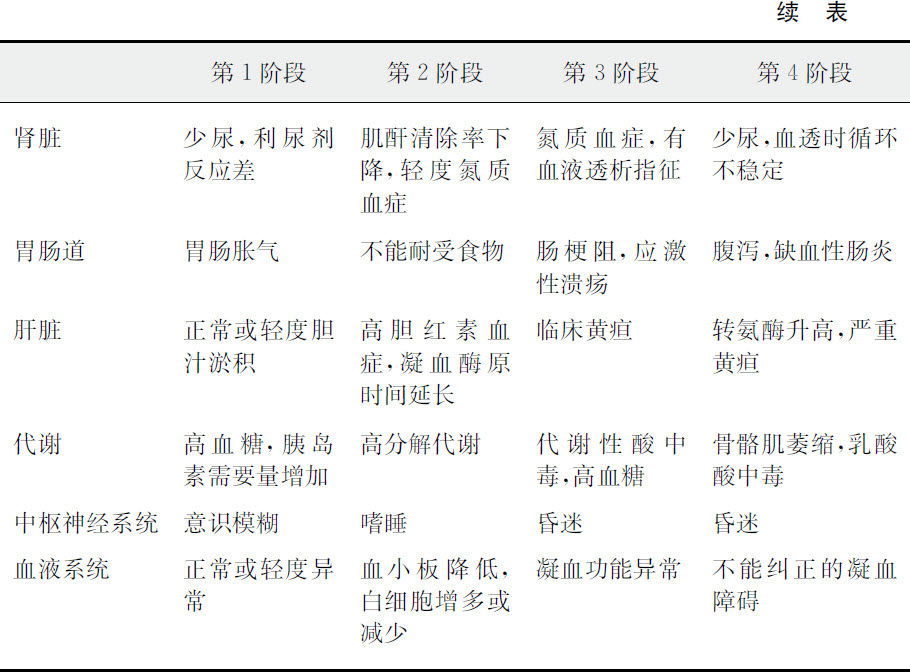
\includegraphics{./images/Image00005.jpg}
\end{table}

{2.预后营养指数(PNI)}
 PNI是由Mullen等对4种营养状态评价参数与外科手术病人预后的相关性进行了分析统计之后提出来的一种综合性营养评价方法。

PNI(%)=158-16.6(ALB)-0.78(TSF)-0.20(TFN)-5.80(DHST)

式中ALB为血清白蛋白(单位:g%);TSF为三头肌皮褶厚度(单位:mm);TFN为血清转铁蛋白(单位:mg%);DHST为迟发性超敏皮肤反应试验(硬结直径>5mm者,DHST=2;硬结直径<5mm者,DHST=1;无硬结反应者,DHST=0)。

评定标准:若PNI<30%,表示发生术后并发症及死亡的可能性均很小;若30%≤PNI<40%,表示存在轻度手术危险性;若40%≤PNI<50%,表示存在中度手术危险性;若PNI≥50%,表示发生术后并发症及死亡的可能性均较大。

Mullen等对161例非急诊手术病人的PNI测定调查显示,手术危险增加与术后并发症发生率及死亡率升高相关,其灵敏度为86%,特异性为69%。

{3.微型营养评定(MNA)}
 是一种简单、快速,适用于评价病人(特别是老年人)营养状况的方法,由Guigoz、Vallas和Garry于1994年提出。MNA评价内容包括: ①人体测量;②整体评定;③膳食问卷;④主观评定等。各项评分相加即得MNA总分。具体评价问卷内容如下所列(见[附])。

\begin{center}\rule{0.5\linewidth}{\linethickness}\end{center}

[附]

营养评价问卷

(一)姓名 性别 出生 年 月 日

(二)家庭住址

(三)原有疾病

(四)体重(kg) 身高(m) 血压(mm Hg)

1.筛选(按不同程度给予量化评分)

(1)既往3个月内是否有食欲下降、消化问题、咀嚼或吞咽困难而摄食减少?

0=食欲完全丧失□ 1=食欲中等度下降□ 2=食欲正常□

(2)既往3个月内体重下降

0=>3kg□ 1=不知道□ 2=1~3kg□ 3=无体重下降□

(3)活动能力

0=需卧床或长期坐着□ 1=能不依赖床或椅子,但不能外出□ 2=能独立外出□

(4)既往3个月内有无重大心理变化或急性疾病?

0=有□ 1=无□

(5)神经心理问题

0=严重智力减退或抑郁□ 1=轻度智力减退□ 2=无问题□

(6)BMI(kg/m\textsubscript{2} )

0=<19□ 1=19~<21□ 2=21~<23□ 3=≥23□

筛选总分(14):≥12正常,无需以下评价;≤11可能营养不良,继续以下评价

2.评价

(1)独立生活(无护理或不住院)?

0=否□ 1=是□

(2)每天应用处方药3种?

0=是□ 1=否□

(3)压疮(褥疮)或皮肤溃疡?

0=是□ 1=否□

(4)每天几次吃完全部饭菜?

0=1餐□ 1=2餐□ 2=3餐□

(5)蛋白质摄入情况:

*每天至少一份奶制品? A是□ B否□

*每周2份以上菜果或蛋? A是□ B否□

*每天肉、鱼或家禽? A是□ B否□

0.0=0或1个“是”□

0.5=2个“是”□

1.0=3个“是”□

(6)每天2份以上水果或蔬菜?

0=否□ 1=是□

(7)每天饮水量(水、果汁、咖啡、茶、奶等):

0.0=<3杯□ 0.5=3~5杯□ 1.0=>5杯□

(8)喂养方式:

0=无法独立进食□ 1=独立进食稍有困难□ 2=完全独立进食□

(9)自我评定营养状况:

0=营养不良□ 1=不能确定□ 2=营养良好□

(10)与同龄人相比,你如何评价自己的健康状况?

0.0=不太好□ 0.5=不知道□ 1.0=好□ 2.0=很好□

(11)中臂肌围(cm):

0.0=<21□ 0.5=21~22□ 1.0=≥22□

(12)腓肠肌围(cm):

0=<31□ 1=≥31□

评价总分(16):

筛选总分:

总分(30):

MNA分级标准:上述各项评分相加,若MNA≥24,表示营养状况良好;若17≤MNA≤23.5,表示存在发生营养不良的危险;若MNA<17,表示有确定的营养不良。

\begin{center}\rule{0.5\linewidth}{\linethickness}\end{center}

{4.住院病人预后指数(HPI)}

HPI=0.92(ALB)-1.00(DH)-1.44(SEP)+0.98(DX)-1.09

式中:ALB为血清白蛋白(单位:g/L);DH为延迟超敏皮肤试验(有1种或多种阳性反应,DH=1;所有均呈阳性,DH=2);SEP:败血症(有败血症,SEP=1;无败血症,SEP=2);DX表示诊断患有癌症(有癌,DX=1;无癌,DX=2)。

评价标准:若HPI为+1,表示有75%的生存概率;若HPI为0,表示有50%的生存概率;若HPI为-2,表示仅有10%的生存概率。

{5.营养风险指数(NRI)}
 美国退伍军人协会肠外营养协作研究组(VATPNCSG)于1991年在《新英格兰医学杂志》上首先提出NRI评价方法。NRI=10.7(ALB)+0.0039(TLC)+0.11(Zn)-0.044(Age)。

式中:ALB为血清白蛋白;TLC为淋巴细胞计数;Zn为血清锌水平;Age为年龄。

评定标准:若NRI>60,表示危险性低;若NRI≤55,表示存在高危险性。

Clugston等于2006年对梗阻性黄疸病人的研究表明,NRI风险升高与住院时间延长和死亡率增加相关。

完整的营养评价包括:疾病及饮食史、体格测量、生化指标、机体组成、营养平衡研究等。在营养评价过程中,体格测量与生化指标是营养评价的最常用方法,具有简单、方便、重复性好、能提供定量资料、不需要特殊仪器等特点。很多测量值与机体组成营养状况分析在统计学上具有显著相关性。然而,简单的体格测量和实验室检查常不能体现营养状况的急性改变,不能反映轻度和中度营养不良,也就不足以作为营养评价的唯一方法。同时,由于置信限较宽,敏感性和特异性差,更适用于流行病学人群调查,评价特定人群的营养状态。近年来,为了提高营养评价方法的敏感性和特异性,人们结合预后和大量的营养学指标,通过多因素回归分析,选择其中有意义的参数,组成最佳的预测模式,建立了多种营养评价方法,为营养状况评价提供了定性、定量的可信指标。

{参考文献}

[1]陶晔璇,徐远飞,汤庆娅,等.儿科病人入院时营养状况评价.中国临床营养杂志,2007,15(4):214~217

[2]蔡威.临床营养基础.第3版.上海:复旦大学出版社,2004,61~18

[3]Tienboon P. Nutrition problems of hospitalised children in a
developing country: Thailand. Asia Pacific J Clin Nutr, 2002, 11 (4):
258~262

[4]Renaudin P. Evaluation of the nutritional status of children less
than 5 years of age in Moundou, Chad: correlations with morbidity and
hospital mortality. Article in French. Med Trop(Mars), 1997, 57 (1):
49~54

[5]Hendricks KM, Duggan C, Gallagher L, et al. Malnutrition in
hospitalized pediatric patients. current prevalence. Arch Pediatr
Adolesc Med, 1995, 149: 1118~1122

[6]Ogden CL, Flegal KM, Carroll MD, et al. Prevalence and trends in
overweight among US children and adolescents, 1999~2000. JAMA, 2002,
288 (14): 1728~1732

[7]Ah SM, Selwyn BJ, Luby S, et al. Prevalence and correlates of
stunting among children in rural Pakistan. Pediatr Int, 2003, 45 (1):
49~53

[8]Jacobs DO, Wong M. Metabolic assessment. World J Surg, 2000, 24
(12): 1460~1467

[9]Phillips SM, Bandini LG, Compton DV, et al. A longitudinal
comparison of body composition by total body water and bioelectrical
impedance in adolescent girls. J Nutr, 2003, 133 (5): 1419~1425

[10]Kuczmarski RJ, Ogden CL, Guo SS, et al. 2000 CDC growth charts for
the United States: methods and development. Vital Health Stat 11, 2002,
(246): 1~190

[11]Ronald E. Pediatric nutrition handbook. 6th ed. American: American
Academy of Pediatrics, 2009, 559~576

\protect\hypertarget{text00003.html}{}{}


\chapter{颅脑}

\section{检查方法}

\subsection{常规检查}

横断面(或轴位)扫描:病人仰卧,有3个主要扫描平面。其扫描基线为:①听眦线(orbitomeatal
line,OML):亦称为眶耳线,简称OM线,即外眦至外耳孔中点的连线。②听眉线(superior
orbitomeatal
line,SML):亦称为上眶耳线,简称SM线,即眉毛上缘中点与外耳孔中点的连线。③瑞氏基底线(reid's
base
line,RBL):亦称人类学基线,简称RB线,即眶下缘与外耳孔中点的连线。检查幕上病变常用OM线;幕下病变常用SM线;眶内病变常用RB线。

冠状面扫描:病人仰卧或俯卧位,头部过伸,使冠状面与OM线垂直扫描。

\subsection{增强扫描}

一般认为,对急性颅脑外伤、急性卒中可只做平扫;对于脑瘤术后复查或只有增强检查才能显示病变的复查病例可只行造影增强;对于脑肿瘤、脑血管疾病、感染性疾病均需做增强扫描,外伤患者平扫正常时亦可行增强扫描。一般造影剂用量为60~100ml或儿童以2ml/kg用量,团注或快速滴注。

其显影机制分为两类:①血管内显影:如动脉瘤、动静脉畸形,其显影时间短,应注药后扫描或边注边扫。②血管外显影:强化机制在于血脑屏障的破坏(如胶质瘤)或血供丰富(如脑膜瘤、听神经瘤、脓肿壁)。由于垂体血供丰富,垂体增强扫描有利于缺乏血供的垂体瘤尤其微腺瘤的检出。

\subsection{脑池造影CT扫描}

造影剂可应用阳性非离子型水溶性碘造影剂(伊索显和欧乃派克等)和阴性造影剂(空气),后者主要用于小听神经瘤的诊断。一般阳性造影剂的用量为8~10ml,空气3~5ml,经腰穿注入。水溶性造影剂取头低脚高位或病变侧在低下部位,气体反之。一般注入造影剂15分钟后扫描,观察脑室多于6小时后扫描,延时的目的在于降低碘液浓度。如欲观察脑脊液的动力变化,则于注入造影剂2小时、6小时、12小时和24小时后进行扫描,必要时可于48小时或72小时后扫描。

\subsection{脑CT血管成像}

脑部CT血管成像或称为脑部CT血管造影(CT
angiography,CTA),是指经静脉注入造影剂后利用CT对包括靶血管在内的受检层面进行连续的薄层立体容积扫描,然后进行图像后处理,最终使靶血管立体显示的血管成像技术。

扫描从后床突下30mm开始,向上达后床突上50~60mm。其常用扫描参数如下:螺距1~2,层厚1~2mm,重建间隔1mm,造影剂用量(300mg/ml)80~120ml,注射流率2.5~3.5ml/s,延迟时间15~25秒。双层或多层螺旋CT可增加螺距、减小层厚,以取得更优质的图像。图像后处理可采用MIP、SSD和VR,以MIP最常用。

脑CT静脉成像(CT venography,CTV)扫描方法同上,只是扫描延迟时间为40秒。

CTA(包括CTV)可用于显示脑底动脉环(willis环)和大脑前、中、后动脉主干及其2~3
级分支血管;CTV
可显示大脑内静脉、大脑大静脉、皮质静脉、上矢状窦、直窦、横窦和乙状窦等。CTA(包括CTV)可用于动脉瘤、血管畸形(主要是AVM)、肿瘤血管、静脉病变及头皮血管瘤等的诊断。

\subsection{脑CT灌注成像}

CT灌注成像在中枢神经系统的应用包括:①作为颅外颈动脉或椎动脉闭塞性疾病的功能性检查方法,研究颅内血流量和侧支循环情况。②早期发现梗死或缺血,并显示其范围。③血管炎或继发性蛛网膜下腔出血时估计血管痉挛情况。④AVM估计分流情况。⑤研究肿瘤的血液灌注情况。

\subsubsection{检查技术}

CT灌注成像的质量受造影剂注射的总量、速度、患者的心功能状态以及CT扫描伪迹、部分容积效应等多种因素的影响。扫描时经肘静脉注射加热至37℃的造影剂40~50ml(儿童约为1ml/kg体重)。开始注射造影剂的同时启动快速动态扫描程序,以1层/秒的速度连续扫30~40秒以上,重建30~40幅灌注图像。注射流率多为8~9ml/s,最快达20ml/s,国内有学者采用2.5ml/s也获得较满意的CT灌注图像。通常包括最大强度投影(MIP)图、脑血流量(CBF)图、脑血容量(CBV)图、局部灌注达到峰值的时间(TTP)等图像。这些图像可通过数字化形式存储,均可彩色显示,以突出病变区域的对比度。

\subsubsection{灌注参数}

1.脑血容量(cerebral blood
volume,CBV):是指存在于一定量脑组织血管结构内的血容量,单位为ml/100g。根据时间-密度曲线下方封闭的面积计算得出。

2.脑血流量(cerebral blood
flow,CBF):CBF=CBV/MTT,指在单位时间内流经一定量脑组织血管结构的血流量,单位为ml/(100g·min)。它反映脑组织的血流量,CBF值越小意味着脑组织的血流量越低。正常值一般>50~60ml/(100g·min),<10~20ml/(100g·min)将导致膜泵衰竭和细胞死亡。

3.平均通过时间(mean transit
time,MTT):开始注射造影剂到时间-密度曲线下降至最高强化值一半的时间,主要反映的是造影剂通过毛细血管的时间,单位为秒(s)。

4.峰值时间(time to
peak,TTP):为开始注射造影剂至强化达到峰值的时间,由时间-密度曲线测得,单位为秒(s)。

此外,还有表面通透性(permeability of surface,PS)等参数。

\section{正常解剖和CT表现}

\subsection{颅盖软组织(头皮)}

颅盖软组织在额、顶、枕部分为皮肤、皮下组织、帽状腱膜、帽状腱膜下层和颅骨骨膜5层。前3层紧密连接,CT不能识别。帽状腱膜下层由疏松结缔组织构成,内含少量血管,CT呈低密度带,头皮裂伤出血亦在此层,如有化脓感染可蔓延到整个颅顶,并可经导静脉扩散到颅内。颅盖软组织在颞部则由皮肤、皮下组织、颞浅筋膜、颞深筋膜、颞肌和颅骨骨膜6层构成。

颅骨外膜CT不能识别,在颅缝处连接紧密并深入缝间成为缝间膜,故骨膜下血肿不超过此缝,并可据此与帽状腱膜下血肿相鉴别。

\subsection{脑颅骨和颅缝闭合的时间及顺序}

脑颅骨由枕骨、额骨、蝶骨、筛骨各一块及颞骨、顶骨各两块组成。颅骨分为3层,即外板、板障和内板。成人内外板CT表现为高密度,CT值>250Hu。新生儿板障为低密度,随年龄增长密度增加,50岁后板障层钙化与内外板融合为一层致密层。成人颅缝宽约0.5
mm。新生儿各骨之间为一片等密度的结缔组织膜相连,称为囟。

颅缝闭合约在30岁以后开始。一般矢状缝先闭合,继为冠状缝。而人字缝和枕骨乳突缝闭合最晚,且可终生不闭合。额缝在出生6个月后开始闭合,而在5~6岁时应完全闭合,此缝亦可终生存在。颅底缝多在出生时闭合,只有蝶枕缝到青春期闭合。

此外,应注意识别脑膜中动脉、板障静脉沟、静脉窦、导静脉、蛛网膜颗粒等常见的脉管压迹,以免误诊为骨折。

\subsection{颅底各颅窝的特点和孔道}

颅底骨内面由蝶骨嵴和颞骨岩部嵴分为前、中、后颅窝。

\subsubsection{各颅窝的结构特点}

1.前颅窝:筛骨板菲薄,外伤易造成骨折、损伤嗅神经及形成脑脊液漏。额骨眶板上面凹凸不平,脑外伤时底部的滑动易引起脑挫伤。

2.中颅窝:孔、洞较多,外伤骨折或肿瘤破坏通过这些结构引起相应的症状。如骨折累及蝶窦出现鼻出血、脑脊液鼻漏;岩锥骨折可损伤面神经和听神经;鼓室盖骨折引起脑脊液耳漏;脑膜中动脉损伤引起硬膜外血肿。

3.后颅窝:有大量肌肉覆盖,骨折较少见。但与颈段相连,可有畸形发生。

\subsubsection{。}

\begin{table}[htbp]
\centering
\caption{颅底主要孔道及内容物}
\label{tab2-1}
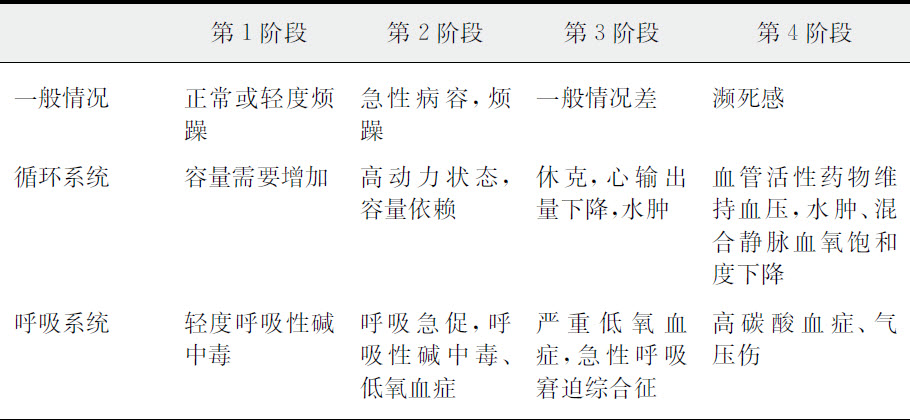
\includegraphics[width=\textwidth,height=\textheight,keepaspectratio]{./images/Image00004.jpg}
\end{table}

\subsection{脑膜}

脑的表面有3层被膜:①软脑膜:紧贴脑的表面,富血管、随脑回起伏。②蛛网膜:位于中层,由薄而透明、疏松成网的纤维构成,无血管结构(故增强扫描无强化),与硬脑膜走行一致。③硬脑膜:位于外层,由致密结缔组织构成,厚而坚韧,与颅骨内面的骨膜完全融合,故通常说硬脑膜为两层结构组成。正常CT不能直接显示3层结构。由于硬脑膜有丰富的血供且无血脑屏障,可以发生明显强化。

硬脑膜内层向颅腔内反折形成双层皱襞有支持、保护作用。主要形成物为:①大脑镰:前端附着于鸡冠,后缘呈水平形与小脑幕相续。大脑镰上、下缘两层分开分别形成上、下矢状窦。轴位像CT呈略高密度线状影,40岁后可钙化。②小脑幕:呈帐篷状分隔大脑枕叶和小脑。后方附着于枕骨横沟,两侧附着于岩椎,上缘正中与大脑镰相续,两侧前内缘形成小脑幕切迹,围绕中脑。轴位呈两侧对称的略高密度影,冠状位呈人字形线状略高密度影。③小脑镰:附着于枕内嵴上的一窄条状突起,分隔小脑半球。④其他:三叉神经半月节(Meckel腔)、海绵窦、直窦、横窦、乙状窦等。

\subsection{蛛网膜下腔和脑池}

脑蛛网膜在脑沟裂处不随之凹入,与软脑膜之间形成宽窄不一的蛛网膜下腔(或称蛛网膜下隙),内含脑脊液。某些局部宽大处称为脑池。主要的有:①大脑纵裂池;②胼胝体池;③小脑延髓池(又称枕大池
);④小脑溪(又称小脑谷);⑤延池;⑥桥池;⑦桥脑小脑角池;⑧脚间池;⑨视交叉池;⑩终板池;⑪外侧裂池;⑫环池;⑬四叠体池;⑭大脑大静脉池;⑮小脑上池(是四叠体池向后的延续);⑯帆间池(又称中间帆腔或第三脑室上池)。

鞍上池为CT和MR等轴位图像所特有。由于扫描体位的影响可呈:①六角星:前角为纵裂前部的后端(紧贴前角后端的横行部分主要是交叉池);两前外侧角为两外侧裂池;两后外侧角为围绕中脑的环池;后角为大脑脚间的脚间池(图\ref{fig2-1})。②五角星:与六角星不同的是,两后外侧角为围绕桥脑上部的桥小脑角池,后角不显示。鞍上池前方是额叶底部直回,两侧壁是颞叶海马钩回,后方为大脑脚或桥脑上部。

\begin{figure}[!htbp]
 \centering
 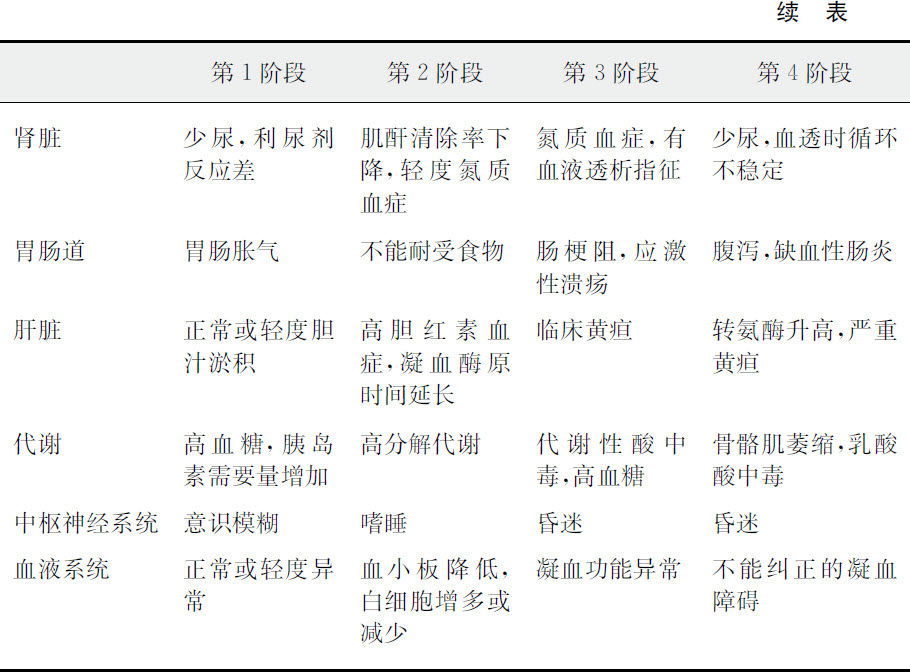
\includegraphics[width=.7\textwidth,height=\textheight,keepaspectratio]{./images/Image00005.jpg}
 \captionsetup{justification=centering}
 \caption{鞍上池 \\{\small 呈六角形水样密度区}}
 \label{fig2-1}
  \end{figure} 



鞍上池内前部可见两条视束,横径约12mm,前后径约8mm,外侧可见两条颈内动脉,中央可见垂体柄,正常垂体柄粗<4mm。

帆间池与第三脑室顶部的区别:帆间池位于第三脑室顶的上方、穹隆体和穹隆连合的下方,呈尖向前的三角区,两前外侧界为穹隆的内侧缘,后界为胼胝体压部。与第三脑室的区别为:①帆间池的层面较第三脑室顶高;②帆间池后界为胼胝体压部,而第三脑室顶部的后界为松果体;③帆间池前部的尖不与侧脑室相连,而第三脑室前端可达侧脑室前角。

此外,枕大池可发育巨大(但一般不产生临床症状)呈对称性和非对称性。结合其有无张力、颅骨有无压迹等可与蛛网膜囊肿相鉴别(图\ref{fig2-2}),有文献将其列入发育异常。因终板较薄不显影,常看到终板池与第三脑室下部相通的假象。小脑溪位于两侧小脑扁桃体之间,呈一细长的间隙,后通小脑延髓池,前通第四脑室。

\begin{figure}[!htbp]
 \centering
 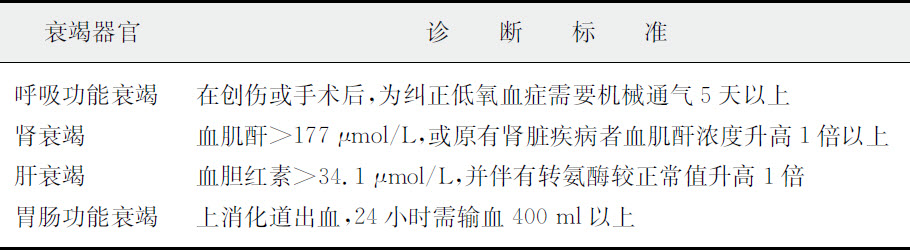
\includegraphics[width=.7\textwidth,height=\textheight,keepaspectratio]{./images/Image00006.jpg}
 \captionsetup{justification=centering}
 \caption{巨大枕大池 \\{\small 显示枕骨内板下至岩锥后缘有新月形水样密度区}}
 \label{fig2-2}
  \end{figure} 


\subsection{大脑半球的分叶及边缘系统}

分叶:大脑由中线的半球间裂分为左右两半,中间由胼胝体相连。大脑半球由脑沟裂分为下列5叶。①额叶:位于前上部。内侧以纵裂和大脑镰与对侧分开,后方由中央沟与顶叶分开,外下方经外侧裂与颞叶分开,前下方为额骨和眶顶。②颞叶:经外侧裂垂直部和水平部与额叶分开。顶枕裂(沟)与枕前切迹(枕极前4~5mm)的连线为颞、枕叶的分界。③顶叶:经中央沟与前方的额叶分开,下方以外侧裂与颞叶分开,后方以顶枕沟与枕叶分开。④枕叶:经顶枕沟与顶叶分开,与颞叶的分界线为顶枕沟与枕前切迹的连线。⑤岛叶:隐藏于外侧裂深部的近三角形的独立区域,四周有环形沟,由额、顶、颞叶皮质沿外侧裂深部凹入形成岛盖。

边缘系统:大脑半球内侧面的扣带回、海马回、钩回、海马、杏仁核等相连构成一个弯弓形脑回,因位置在大脑和间脑交界处的边缘,所以称为边缘系统或边缘叶。通过控制下丘脑来调节内脏及情绪活动。

此外,颞、顶、枕叶的分界线是假设的,因此很不清楚,这一区域也称为颞顶枕交界区。

\subsection{大脑半球的白质}

\subsubsection{半卵圆中心}

髓质占大脑半球的大部分,较厚的皮质下纤维在横断面图像、侧脑室上层面呈半卵圆形,故称为半卵圆中心,是影像学的一个概念。

\subsubsection{大脑白质纤维分类}

大脑白质的纤维结构复杂,大体分为以下3种:

1.联络纤维:在一侧半球内部各回、各叶间的往返纤维称为联络纤维。短的是联系在相邻脑回之间的弓状纤维;长的是联系在各叶皮质间的纤维,如钩束、扣带束、上纵束、下纵束及枕额上、下束等。

2.连合纤维:指联系左右半球的纤维,主要有胼胝体、前联合和海马联合等。①胼胝体:位于大脑纵裂底部,呈拱桥状。前端弯向腹后方称嘴,由嘴向前上方弯曲部称为膝,由膝向后延伸为体部(构成侧脑室壁的大部分),后端较厚称为压部。②前联合:位于胼胝体嘴的后下方,呈卵圆形,是两半球的嗅球和海马旁回的联合。

3.投射纤维:大脑皮层与其下部的间脑、基底节、脑干和脊髓的连接纤维称为投射纤维。包括内囊、穹隆、外囊和最外囊。①内囊:两侧内囊横断面呈“><”型,中央顶点为膝,前后分别为前肢和后肢。内囊位于丘脑、尾状核和豆状核之间。内囊后肢边缘模糊的低密度区(约位于膝部到豆状核后缘距离的2/3~3/4处)为正常皮质脊髓束,勿误为缺血灶。②外囊:在豆状核外,居豆状核和屏状核之间,两侧在横断面呈“()”型。③最外囊:位屏状核外侧,岛叶内侧,CT难以显示。

\subsection{基底节}

基底节包括尾状核、豆状核、屏状核和杏仁核。其中豆状核有两个白质板将其分为3部分,外部最大称为壳,内侧两部分称为苍白球。但CT不能显示其白质板。尾状核和豆状核合称为纹状体,与维持肌张力及运动频率有关。杏仁核与情绪变化有关。

\subsection{间脑}

间脑(通常将端脑和间脑合称为大脑)连接大脑半球和中脑,包括以下4部分。

1.丘脑:为一大卵圆形核团。内侧构成侧脑室侧壁,借中间块使左右丘脑相连;其外侧为内囊后肢;其前端尖圆为丘脑结节;后端圆钝为丘脑枕;丘脑枕的外下部有两个隆起为内、外侧膝状体。丘脑是各种感觉体传向大脑皮层的中间站。

2.下丘脑:构成侧脑室底和侧壁的一部分,包括视交叉、漏斗、灰结节、乳头体和垂体神经部。它是皮质下植物神经中枢,并通过下丘脑---垂体柄和垂体门脉系统调节垂体功能。

3.底丘脑:为丘脑和中脑的移行区。接受来自苍白球和运动区的纤维,并发出纤维到达红核、黑质及中脑被盖,功能上与苍白球密切相关。

4.上丘脑:位于三脑室后部,包括丘脑髓纹、缰三角和松果体,参与嗅反射通路。松果体为一退化的内分泌结构,分泌抑制青春期激素。松果体呈锥形,长5~8mm,宽4mm,向左偏移1~2mm是正常现象,但向右偏移却有病理意义。CT扫描75%以上成人于三脑室后部可显示松果体与缰联合钙化。缰联合钙化居前,范围不超过1cm;松果体钙化居后,一般不超过5mm。

此外,有文献将内、外侧膝状体称为后丘脑。

\subsection{脑干}

脑干上接间脑,下续颈髓,与小脑之上、中、下脚相连,分为以下3部分。

1.中脑:在间脑和脑桥之间,从前向后为大脑脚、被盖和四叠体(顶盖)组成。大脑脚与被盖之间以黑质为界;被盖与四叠体之间以中脑导水管为界。腹侧两束粗大的纵行纤维为大脑脚,其间形成脚间窝,动眼神经从脚间窝出脑。中脑背部有上丘和下丘两对隆起总称为四叠体。上、下丘分别与外、内侧膝状体借上、下丘臂相连,分别是皮质下视觉和听觉反射中枢。下丘后方连接前髓帆,滑车神经自下丘下方发出。

2.桥脑:桥脑在中脑的下方,从前向后为基底部和被盖部。前面正中浅沟内可见基底动脉。横行基底部的纤维向两侧聚成脑桥臂,经小脑中脚进入小脑。基底部与桥臂之间有三叉神经发出。桥脑腹侧与延髓交界的沟内,由内向外有外展神经、面神经和前庭蜗神经发出。桥脑背面下半部即菱形窝的上半部为第四脑室底(CT轴位第四脑室前为桥脑)。

3.延髓:上接桥脑,下续颈髓。腹侧面中线(前正中裂)两旁有锥体(由皮质脊髓束和皮质脑干束组成)。在延髓的下方由纤维交叉形成锥体交叉。锥体外侧有椭圆形隆起称为橄榄。锥体和橄榄之间有舌下神经穿出。橄榄背侧自上而下依次有舌咽神经、迷走神经和副神经根发出。

\subsection{小脑和小脑核}

小脑位于桥脑和延髓的后方,中间相隔第四脑室。小脑正中的蚓部与两侧小脑半球间无明显分界。小脑半球下面近枕骨大孔部分突出称为小脑扁桃体。小脑前后均向内凹称为小脑前切迹和后切迹。小脑半球借上、中、下脚分别与中脑背侧、桥脑腹侧和延髓的背侧相连接,小脑表面为灰质,内部为白质。

小脑白质内有灰质团块,称为小脑中央核。共有4对,分别为齿状核、顶核、栓状核、球状核。其中齿状核最大,位于小脑半球的中心部,是小脑传出纤维的主要发起核。

\subsection{脑室系统}

1.侧脑室:左右各一,分为以下5部分:①前角:又称额角,位于额叶内,在室间孔以前。顶为胼胝体,内侧壁是透明隔,倾斜的底及外侧壁为尾状核头。②体部:位于顶叶内,由室间孔至三角部。顶为胼胝体体部;内侧壁是透明隔;底由外侧到内侧分别为尾状核体、丘脑背面终纹、丘脑上面的外侧部、脉络丛和穹隆外侧缘。③三角区:即体、后角、下角分界处,内容脉络球。CT上是区分颞、枕、顶叶的标志。④后角:又称枕角,位于枕叶内,形状变异很大,有时缺如。顶和外侧壁由胼胝体放散形成;内侧壁上有两个纵行膨大,上方的称后角球(由胼胝体大钳构成),下方的称禽距。⑤下角:在颞叶内,又称颞角。在丘脑后方弯向下,再向前进入颞叶。顶大部分由胼胝体构成,内侧小部分由尾状核尾和终纹构成,底由内至外为海马伞、海马和侧副隆起。

正常成人两侧前角之间的距离<45mm,前角间最大距离与头颅最大内径之比<35%,在2岁以下其比值应<29%,两侧尾状核内缘之间的距离<25mm,为15mm左右。

2.第三脑室:两侧间脑间的狭窄腔隙。成人男性宽为2.8~5.9mm,女性为2.5~5.3mm。经室间孔与左右侧脑室相通,后经中脑导水管与第四脑室相通。顶有第三脑室脉络丛;底为下丘脑;前壁为前联合和终板;后壁为缰联合、松果体和后联合。

3.第四脑室:腹侧为桥脑和延髓,背侧为小脑,上接中脑导水管,下续脊髓中央管。经侧孔与桥脑小脑角池相通;经下端正中孔与小脑延髓池相通。第四脑室底为菱形窝,顶为前髓帆和后髓帆,呈马蹄形,宽(前后径)约9mm。

4.中脑导水管:位于中脑背侧,是中脑被盖和四叠体的分界,长约7~18mm,直径约1~2mm。正常CT难以显示。

此外,第五、第六脑室即透明隔间腔和穹隆间腔属两种解剖变异。但第五脑室如积液过多,向外膨隆并影响室间孔的引流,可称为透明隔囊肿。

\subsection{静脉和静脉窦}

\subsubsection{脑动脉}

脑的血供来自颈内动脉和椎动脉,前者供应大脑半球的前2/3,后者供应脑干、小脑和大脑半球的后1/3。

1.大脑前动脉:供应额、顶叶近中线内侧面约1.5cm的范围,呈长条形。其水平段分出细小前穿质动脉供应尾状核头、壳核和内囊前部,另有部分供应下丘脑。

2.大脑中动脉:皮质支供应额、顶、颞叶的外表面大部分。中央支供应尾状核和壳核的一部分,以及苍白球、内囊前后肢,称为豆纹动脉。

3.大脑后动脉:供应枕叶和颞叶底面,中央支供应部分间脑。

4.椎基动脉:两侧椎动脉在延髓腹侧汇合为基底动脉。基底动脉走行于桥脑前面,到脚间池分为左右大脑后动脉。基底动脉分出成对的桥脑支、内听道支、小脑前支和小脑上支。小脑后支来自椎动脉。

颅底动脉环即Willis环,由前交通动脉、两侧大脑前动脉、两侧后交通动脉和大脑后动脉相互吻合构成的六角形动脉环,是沟通两侧颈内动脉和椎动脉的侧支循环通路。其变异较大,完整者仅占53.8%。

\subsubsection{脑静脉}

大脑半球静脉分为深、浅两组。①浅静脉:收集大脑皮质和白质浅层的静脉血,包括大脑上静脉、大脑中静脉和大脑下静脉分别汇入上矢状窦、海绵窦、横窦、岩上窦和岩下窦,其间有吻合静脉相沟通。②深静脉:主要收集脑深部的血液。透明隔静脉和纹丘静脉在室间孔后缘汇合成大脑内静脉,两侧的大脑内静脉以及基底静脉在松果体后方汇合成大脑大静脉。大脑大静脉与下矢状窦相连终于直窦。

\subsubsection{静脉窦}

在两层硬脑膜之间引流静脉血液入颈内静脉,包括上矢状窦、下矢状窦、直窦、横窦、海绵窦、岩上窦、岩下窦和乙状窦。其中海绵窦位于蝶鞍两侧高约5~8mm,横径5~7mm,前后径为10~15mm,增强后呈高密度,平扫不易显示。

\subsection{Brodmann功能定位区和大脑皮质的主要功能区}

正常脑皮质的密度高于髓质,易于分辨。脑皮质CT值为32~40Hu,脑髓质CT值为28~32Hu,两者平均相差(7.0±1.3)Hu。含脑脊液的间隙为水样密度,CT值为0~20Hu。

图\ref{fig2-3}A~I为正常颅脑CT轴位像,按Brodmann功能定位法共分47个区。如图\ref{fig2-3}A~I和图\ref{fig2-4}A、B、C、D所示,大脑皮质主要的功能区定位如下:

1.第Ⅰ躯体感觉区:位于中央后回和中央旁小叶的后半,主要是3、1、2区。

2.第Ⅰ躯体运动区:位于中央前回和中央旁小叶的前半,主要是4区。

3.视觉区:位于枕叶内侧面,距状裂(沟)两侧,包括舌回和楔叶的一部分,即17、18、19区。

4.听区:位于颞横回,主要是42区,接受听辐射的投射。其特点是一侧听区接受双侧的听觉冲动传入,但以对侧为主。故一侧听区损伤,可使双侧听力下降,但不会完全耳聋。

5.味觉区:在中央后回下端。

6.语言中枢:在左侧半球的皮质产生了4个分析区,总称为语言中枢。①说话中枢:在额下回后部,即44区。此区损伤产生失语症。②书写中枢:位于额中回后部。此区损伤产生失写症。③阅读中枢:位于顶下小叶的角回,即39区。此区损伤产生失读症。④听话中枢:在颞上回后部。功能是理解别人的语言和监听自己所说的话。此区损伤,对听到的语言不能理解,自己说话错误、混乱而不自知,称为感觉性失语症。

7.其他:5、7区为触摸识别物体的实体感觉皮质区,为顶上小叶。额上回从前向后为9、8、6区。8区和枕叶19区为皮质眼球运动区,受刺激时产生双眼向对侧同向偏盲。8和6区为锥体外系皮质区,与共济运动有关。9、10、11区为额叶联合区,与智力和精神活动密切相关。40区位于顶下小叶缘上回,优势半球为运用中枢,是人类后天经复杂的动作和劳动技能所建立的运动区。损伤后,手的运动功能正常,但不能完成过去掌握的复杂动作和操作技法。


\begin{figure}
  \centering
  \subfloat[经海绵窦层面]{
  \begin{minipage}[b]{0.7\textwidth}
    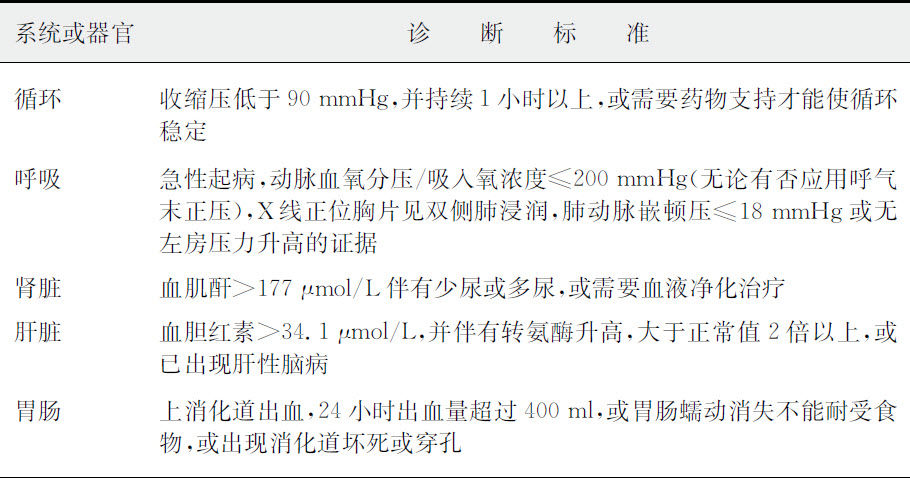
\includegraphics{./images/Image00007.jpg}
  \end{minipage}}\\
  \subfloat[经鞍上池层面]{
  \begin{minipage}[b]{0.7\textwidth}
    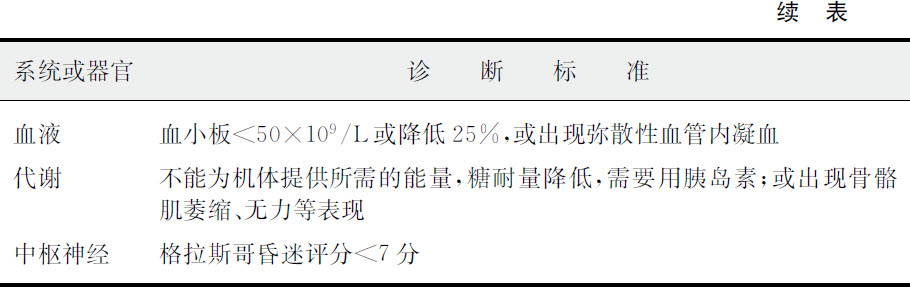
\includegraphics{./images/Image00008.jpg}
  \end{minipage}}\\
  \subfloat[经三脑室下部层面]{
  \begin{minipage}[b]{0.7\textwidth}
    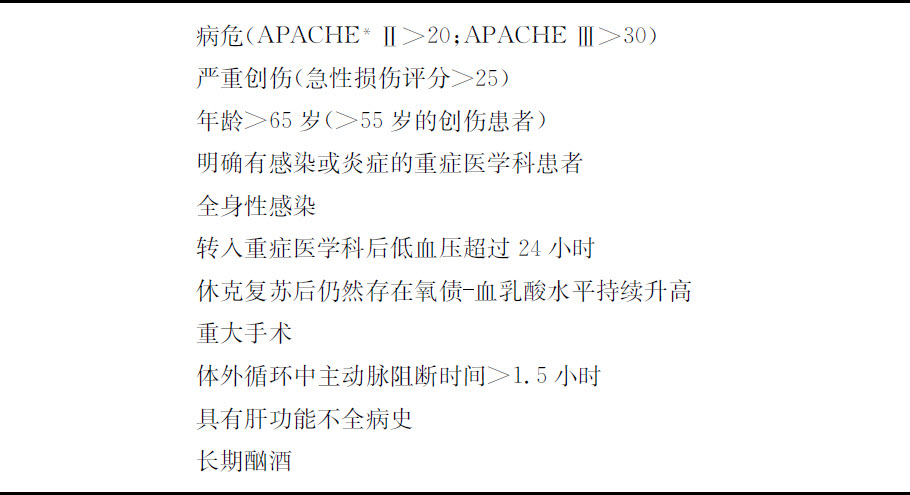
\includegraphics{./images/Image00009.jpg}
  \end{minipage}}
  \caption{}
  \label{fig2-3}
  \end{figure}

  \begin{figure}
    \ContinuedFloat             %%<-- put this in subsequest figures.
    \centering
    \subfloat[经松果体层面]{
      \begin{minipage}[b]{0.7\textwidth}
        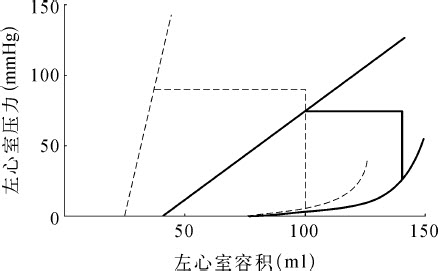
\includegraphics{./images/Image00010.jpg}
      \end{minipage}}\\
      \subfloat[经三脑室上部层面]{
      \begin{minipage}[b]{0.7\textwidth}
        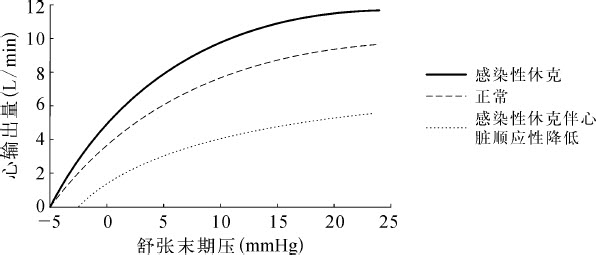
\includegraphics{./images/Image00011.jpg}
      \end{minipage}}\\
      \subfloat[经侧脑室体部层面]{
      \begin{minipage}[b]{0.7\textwidth}
        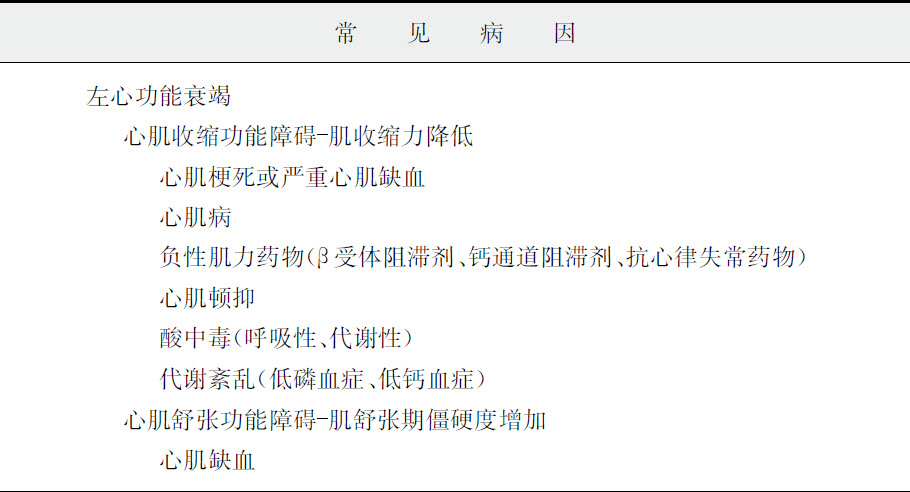
\includegraphics{./images/Image00012.jpg}
      \end{minipage}}
      \caption[]{}
  \end{figure}

  \begin{figure}
    \ContinuedFloat             %%<-- put this in subsequest figures.
    \centering
    \subfloat[经胼胝体体部层面]{
      \begin{minipage}[b]{0.7\textwidth}
        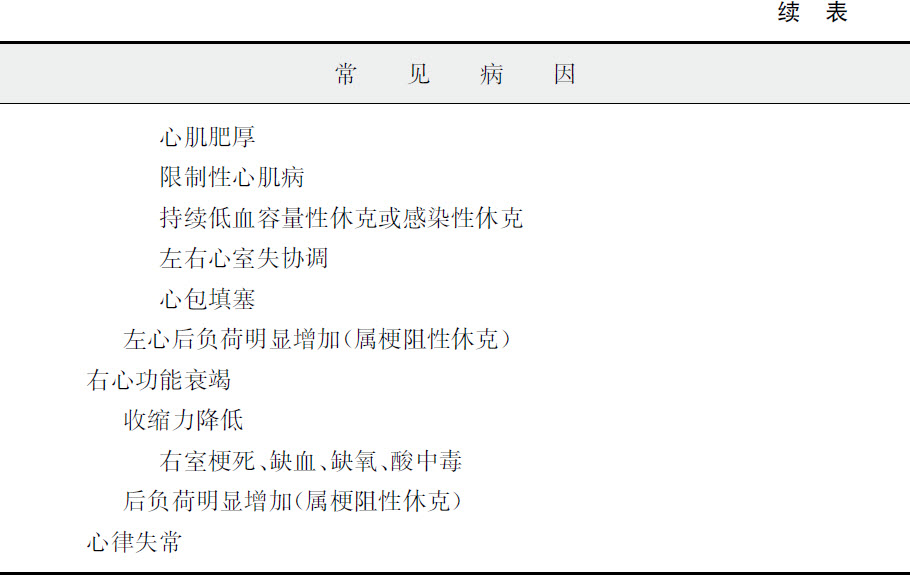
\includegraphics{./images/Image00013.jpg}
      \end{minipage}}\\
      \subfloat[半卵圆中心层面]{
      \begin{minipage}[b]{0.7\textwidth}
        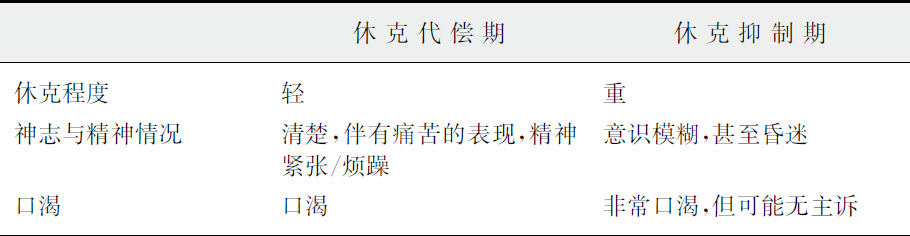
\includegraphics{./images/Image00014.jpg}
      \end{minipage}}\\
      \subfloat[半卵圆中心以上层面]{
      \begin{minipage}[b]{0.7\textwidth}
        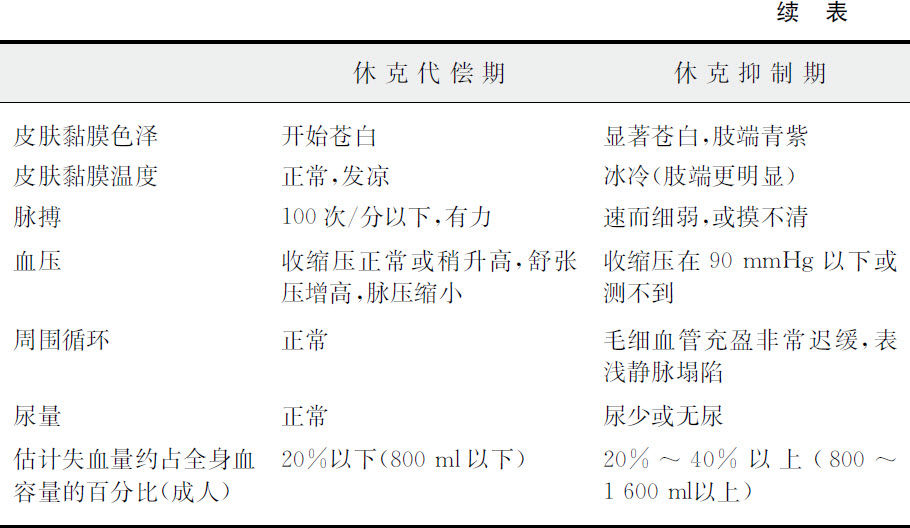
\includegraphics{./images/Image00015.jpg}
      \end{minipage}}\\
      \caption[]{}
  \end{figure}

  \begin{figure}
    \centering
    \subfloat[大脑半球外侧面的主要沟回]{
    \begin{minipage}[b]{0.7\textwidth}
      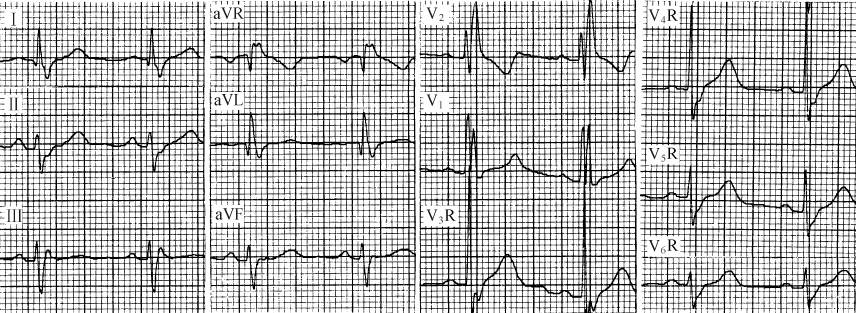
\includegraphics{./images/Image00016.jpg}
    \end{minipage}}\\
    \subfloat[大脑半球内侧面的主要结构]{
    \begin{minipage}[b]{0.7\textwidth}
      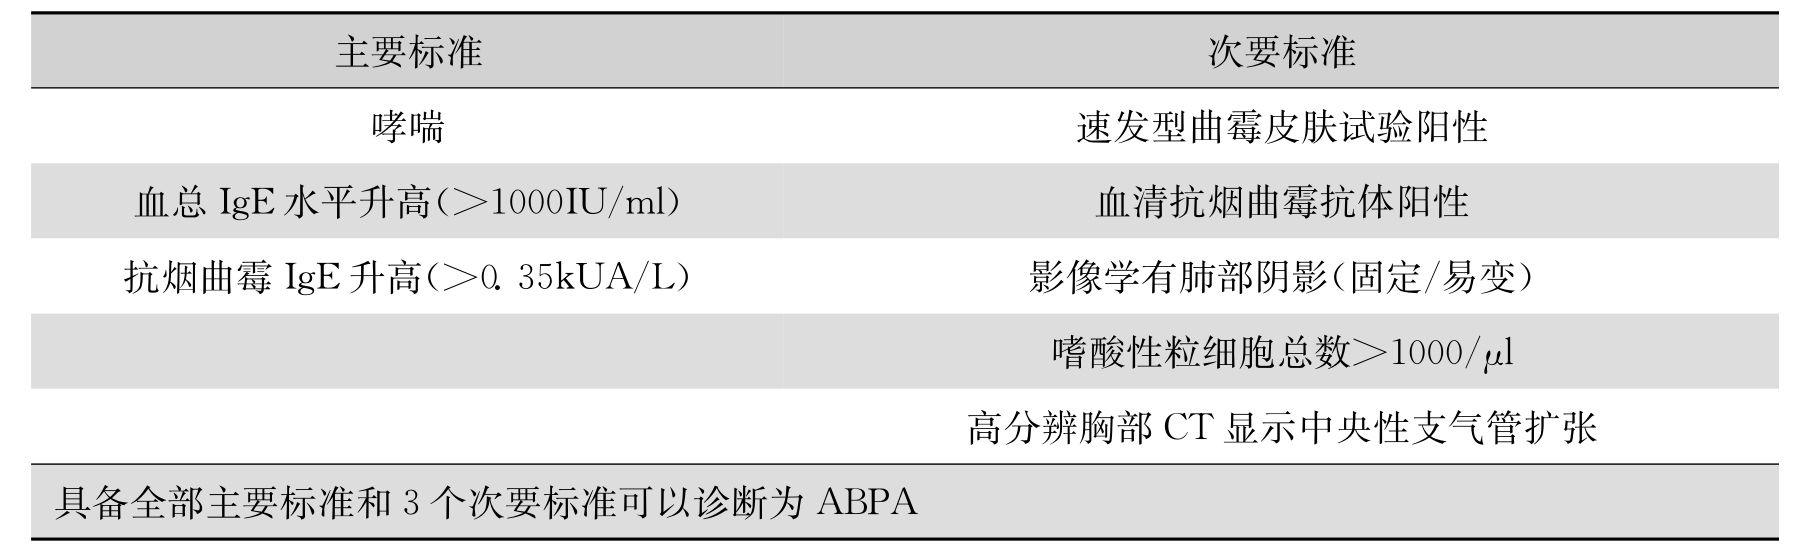
\includegraphics{./images/Image00017.jpg}
    \end{minipage}}\\
    \caption{}
    \label{fig2-4}
    \end{figure}

    \begin{figure}
      \ContinuedFloat             %%<-- put this in subsequest figures.
      \centering
      \subfloat[大脑半球背外侧面功能分区示意图]{
    \begin{minipage}[b]{0.7\textwidth}
      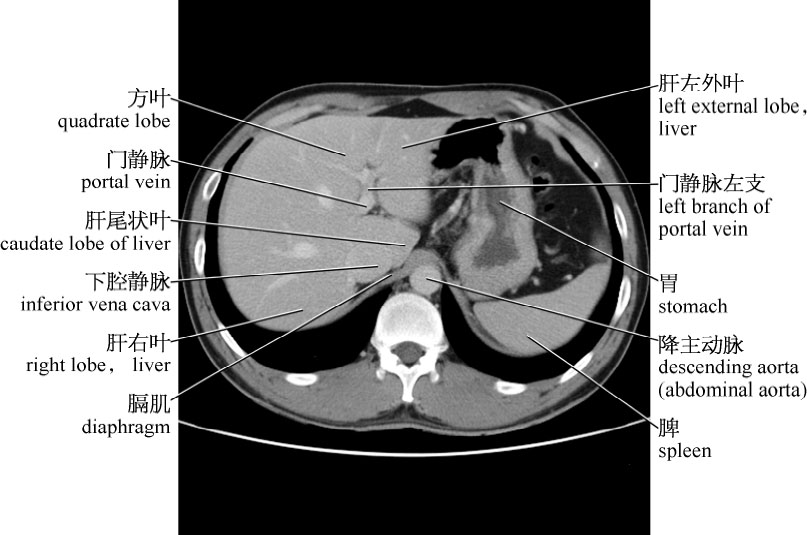
\includegraphics{./images/Image00018.jpg}
    \end{minipage}}\\
    \subfloat[大脑半球内侧面功能分区示意图]{
    \begin{minipage}[b]{0.7\textwidth}
      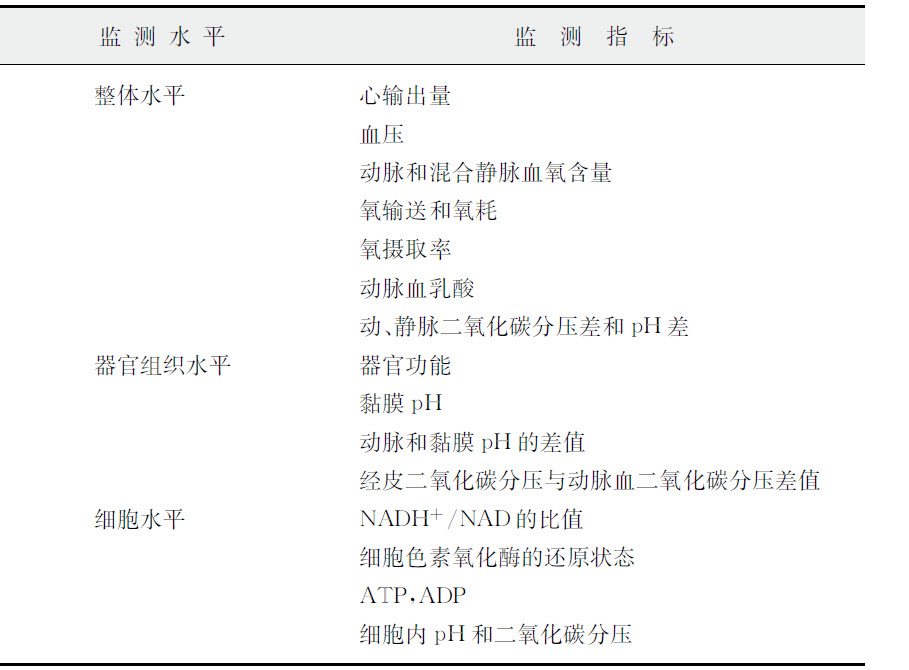
\includegraphics{./images/Image00019.jpg}
    \end{minipage}}\\
        \caption[]{}
    \end{figure}

\section{先天颅脑发育畸形和变异}

\subsection{概述}

所谓畸形是指胚胎期或胎儿期发生的脏器、系统或全身的形态异常或形成异常,不包括出生时的损伤和生后发育成长中产生的障碍。

先天性颅脑发育畸形的发病原因是由于胚胎期神经系统发育异常所致,约40%为遗传因素和子宫内环境的共同影响所致。前者包括染色体变异、显性或隐性遗传;后者包括宫内缺氧、感染等。其余60%病因复杂,机制不详。目前,可分为以下3大类:

1.器官形成障碍:①神经管闭合障碍:以脊髓脊膜膨出最常见,主要包括颅裂畸形(脑膜膨出、脑膨出、无脑畸形)、小脑扁桃体延髓联合畸形(Chiari畸形)、胼胝体发育不全、胼胝体脂肪瘤、先天性四脑室中侧孔闭锁(Dandy-Walker综合征)。②脑裂形成障碍:前脑无裂畸形(单叶、半叶、全叶)、视隔发育不良。③神经元移行异常:又称脑沟及细胞移行障碍,主要包括脑裂畸形、无脑回、灰质异常(巨脑回、多微脑回、灰质异位)。④大小异常:包括脑大、脑小畸形。⑤破坏性病变:包括积水性无脑畸形、脑穿通畸形。

神经管闭合不全是指胚胎期神经沟发育形成神经管的过程中,由于发育障碍而造成神经系统及其周围结构缺陷的一类中枢神经系统先天畸形,可能与孕妇叶酸缺乏有关。除表现出神经症状和体征外,更为常见的是周围组织的异常,包括颅骨、脑膜、椎体及其附件、皮肤和皮下组织(如先天性皮毛窦)等。该类疾病相当常见,其中尤以脊柱的畸形为多,是脑部的10倍或更多。

大脑皮层的神经元来自胚胎时期的脑室壁即神经管上皮。胚胎第6周末神经管经分化形成4个胚胎带,由内向外分别为脑室带、脑室下带、中间带和边缘带。脑室带和脑室下带的细胞具有分化成各类神经元的功能,故又称为生发基质层。胚胎7周时生发基质层的成神经细胞逐渐向外移行,大部分穿过中间带在边缘带内分化成神经元,形成有6层结构的正常脑皮质。26~30周脑回完全形成。神经元移行的过程复杂漫长,此间受到干扰则造成移行障碍。临床均以癫痫、智力障碍为最常见症状。

2.组织发生障碍:总体脑结构正常,但有异常细胞存在并持续分化。①神经皮肤综合征:包括神经纤维瘤病、脑颜面血管瘤病(Sturge-Weber综合征)、结节性硬化、视网膜小脑血管瘤病(又称Von
Hippel-Lindan病)。②血管性病变。③先天性肿瘤。

3.细胞发生障碍:①先天性代谢异常:包括氨基酸尿症、黏多糖沉积病、脂质沉积病等。②脑白质营养不良。③神经元变性。④轴索营养不良。

\subsection{脑膜膨出和脑膜脑膨出}

本病即显性颅裂畸形或称囊性颅裂畸形。临床可见颅外软组织肿物,大多于出生时即可发现。如仅有颅骨缺损,而无内容物自缺损处膨出称为隐性颅裂。

\textbf{【病理】}
颅裂多发生于中线或中线旁(斜坡除外),硬膜常缺如。脑膜(软膜和蛛网膜)或(和)脑突出于脑外,严重时可含部分脑室,可合并其他神经管闭合障碍(如Chiari畸形、胼胝体发育不全)等畸形。

\textbf{【临床表现】}
囊性肿物与头部相连,于出生时即可发现,也可于生后几个月或几年发现。哭闹或咳嗽时肿物增大,张力增加;压迫肿物,则前囟突出;局部可扪及骨缺损的边缘。一般无神经系统症状,也可表现为智力低下、抽搐及脑损害表现。

\textbf{【CT表现】}
软组织疝出的部位可见边缘硬化的颅骨缺损,枕部占70%,顶部占10%~20%,额上部占10%,颅底部占10%。应注意向颅外膨出的软组织,是否含有脑脊液和脑组织;颅底部膨出应注意与鼻息肉或鼻咽部肿瘤相鉴别(图\ref{fig2-5}\footnote{16岁女性,枕骨局限缺损,可见疝出之少量软组织密度灶})。同时,可合并胼胝体缺失、Chiari畸形、灰质异位等畸形。

\begin{figure}[!htbp]
 \centering
 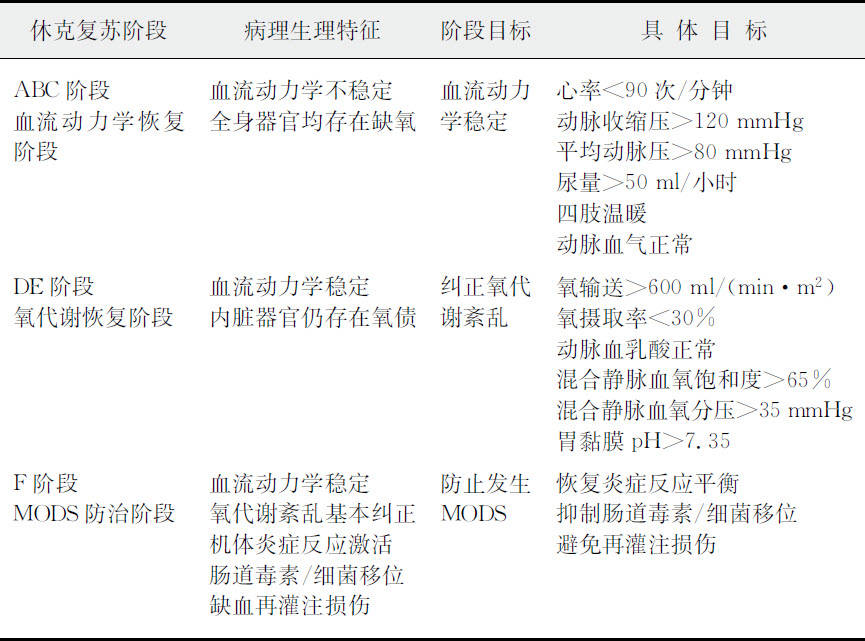
\includegraphics[width=.7\textwidth,height=\textheight,keepaspectratio]{./images/Image00020.jpg}
 \captionsetup{justification=centering}
 \caption{脑膜脑膨出}
 \label{fig2-5}
  \end{figure} 

\subsection{小脑扁桃体延髓联合畸形}

本病又称Chiari畸形,为后脑先天性发育异常。扁桃体过长、变形,经枕大孔疝入上段颈椎管,延髓和第四脑室可同时向下延伸。常伴脊髓空洞症、脊髓纵裂、脑积水和颅颈部畸形等。

\textbf{【病理】} 可分为以下4型。

Ⅰ型:多见。最可能的发病机制是胚胎枕节发育不良导致后颅窝狭小,难以容纳正常发育的后脑,使小脑扁桃体下疝。小脑扁桃体与小脑下部疝入颈椎管上端,无延髓移位。一般认为小脑扁桃体下端低于枕大孔≥5mm为下疝,<3mm为正常,二者之间临床意义不确定。通常不伴其他脑畸形,临床可无症状,或有轻度运动障碍和小脑症状。

Ⅱ型:最常见。小脑扁桃体和蚓部同时疝出枕大孔,脑桥下部及延髓下移,第四脑室延长。几乎总是伴有某种神经管闭合不全如脑膜膨出、脊髓脊膜膨出(腰骶部多见)、脑积水和脊髓空洞症。常有上述Ⅰ型症状。

Ⅲ型:十分罕见。为Ⅱ型伴有低枕部或高颈部脑膜脑膨出,临床症状较Ⅱ型更严重。

Ⅳ型:非常罕见。伴有严重的小脑发育不良,结构独特,可能不单独存在。该型归为小脑发育不良可能更合适。

\textbf{【临床表现】}
本病可无症状,尤其畸形轻者可无,也可直到成年甚至50~60岁始有症状。神经损害症状主要是颅神经和颈神经受损、延髓和上颈髓受压,可有小脑症状、颅内高压及脊髓空洞症表现。

\textbf{【CT表现】}
CT可显示下列特征:①小脑扁桃体、小脑蚓部及小脑、脑干和第四脑室下移;②脑积水;③大脑镰和天幕发育不良;④部分脑组织过度增生或脑发育异常导致脑室系统畸形;⑤后颅窝内容物的挤压引起的颅骨和蛛网膜下腔的改变。但只有通过脑池造影CT扫描或MR显示扁桃体下移、其下端变尖才能明确诊断。

\subsection{侧孔先天性闭锁}

本病又称Dandy-Walker综合征,第四脑室正中孔、外侧孔闭锁为发病主要原因。

\textbf{【病理】}
此病是一组先天性后脑发育畸形,包括脑积水、小脑发育障碍(小脑蚓部不发育或发育不全,约25%蚓部缺如)和与第四脑室相通的巨大后颅窝囊肿。囊肿大小变化很大,囊壁由下髓帆组成,包括室管膜、胶质、小脑组织、软脑膜和蛛网膜等,囊壁可钙化,可合并大脑发育异常。

\textbf{【临床表现】}
男女发病率相近。大多于2岁前产生症状,常因运动发育迟缓而就诊。部分因颅内高压或小脑症状而就诊,头颅明显增大。

\textbf{【CT表现】}
在出生时脑积水是不常见的,75%在生后3个月出现。典型者小脑蚓部体积变小或缺如,小脑半球分离;巨大的后颅窝“囊肿”与扩大的第四脑室相通。脑干前移,桥前池、桥小脑角池消失,后颅窝扩大,枕骨变薄,天幕上移。可合并胼胝体发育不良、多微脑回、灰质异位、枕部脑膨出等。

\textbf{【鉴别诊断】}
①后颅窝巨大蛛网膜囊肿:第四脑室与囊肿不相通,而是受压前移,必要时通过脑池造影CT鉴别。②巨大枕大池:第四脑室无受压,无蚓部发育不全、无后颅窝扩大等,但与下蚓部几乎完整的Dandy-Walker畸形不易鉴别。上述两者均可偶有轻度脑积水,但小脑发育基本正常。

\subsection{Joubert综合征}

\textbf{【病理】}
病理特征是小脑蚓部不发育或发育不全而形成异常的“中线裂”,还有小脑齿状核的变形、下橄榄核和旁橄榄核的发育不良、背侧柱核的异常以及锥体交叉缺如。

\textbf{【临床表现】}
男性多见,有发作性呼吸过度和(或)呼吸暂停、眼球活动异常(眼球震颤、斜视等)和儿童期发育迟缓。还可伴有其他异常如小头畸形、面部畸形、胼胝体发育不全、多指畸形和先心病等。

\textbf{【CT表现】}
在桥脑和中脑连接水平,第四脑室呈“蝙蝠翼状”。于第四脑室底部紧贴小脑半球中线处可见小脑半球间形成的切迹即“中线裂”。小脑上脚增粗,由于交叉的缺乏而向外分开,并导致中脑背侧局部缺失,形成所谓的“磨牙征”。第四脑室中部呈倒立三角形状,与不连接的小脑半球间的脑脊液间隙相连形成“酒杯状”表现,无后颅窝囊肿和脑积水。

\subsection{胼胝体发育不全}

\textbf{【病因病理】}
胼胝体在妊娠12~20周时形成。本畸形偶然发病,病因一般不明,多为先天性。在某些病例中,母体的血管性、外伤性、中毒性或感染性损伤为致病因素。产期缺血缺氧性损害也可引起获得性胼胝体发育不全。本病可为全部或部分缺如,常伴发其他畸形(最高达50%),如前脑无裂畸形、多微脑回、厚脑回、灰质异位、脑小畸形、视隔发育不良、胼胝体脂肪瘤或纵裂池蛛网膜囊肿等。

\textbf{【临床表现】}
临床症状各不相同,视伴发的其他神经系统畸形而定。许多患者可无症状或仅有轻度视觉障碍;或有交叉触觉定位障碍而智力正常;严重者可有癫痫和智力不全。

\textbf{【CT表现】}
由于胼胝体完全或部分缺如而表现不一。可见纵裂池前部明显向后伸展,靠近第三脑室前壁。侧脑室额角和体部间距增大,而且两侧脑室平行分离,并可见其内壁呈弓形外突,冠扫额角呈“八”字形分离。枕角不对称性扩大(憩室),第三脑室轻度扩大并上移。正常时,两侧脑室的脉络丛常在室间孔间会聚,并形成45\textsuperscript{o}
~70\textsuperscript{o} 夹角,本病此夹角多<35\textsuperscript{o}
~40\textsuperscript{o}
(图\ref{fig2-6}\footnote{A~D为同一患者,可见纵裂池前部明显向后伸展,靠近第三脑室前壁;第三脑室轻度扩大并上移;侧脑室额角和体部间距增大,两侧脑室平行分离}),有时可见半球间裂(纵裂池)的蛛网膜囊肿等畸形。本病应注意与脑室周围白质软化症(PVL)相鉴别。



\begin{figure}[!htbp]
 \centering
 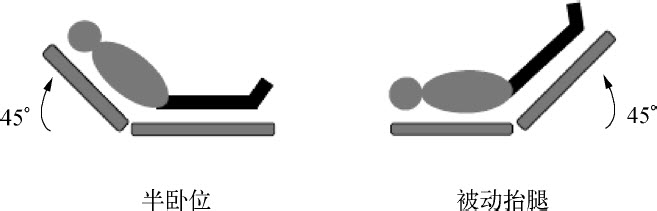
\includegraphics[width=\textwidth,height=\textheight,keepaspectratio]{./images/Image00021.jpg}
 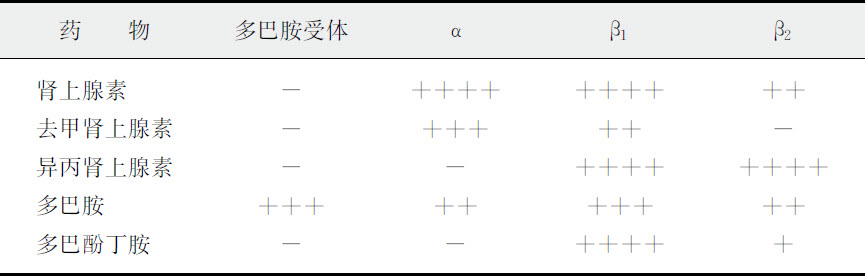
\includegraphics[width=\textwidth,height=\textheight,keepaspectratio]{./images/Image00022.jpg}
 \captionsetup{justification=centering}
 \caption{胼胝体发育不全}
 \label{fig2-6}
  \end{figure} 


\subsection{前脑无裂畸形}

本病又称全前脑畸形,是胚胎发育过程中由前脑发育障碍引起的一组复杂的颅脑与面部畸形。

\textbf{【病因病理】}
其病因不明,部分为常染色显性和隐性遗传。大脑不能分裂成两侧大脑半球,有时也不能在横向上分裂成端脑和间脑,可分为无脑叶型、半脑叶型、脑叶型3种类型,代表了畸形的不同程度。

\textbf{【临床表现】}
男女发病相近,因婴儿多数死于流产或出生后不久,故临床少见。脑叶型可活到成年,并有运动迟缓、智力低下等神经精神症状。

\textbf{【CT表现】} 3种类型分别表现如下。

1.无脑叶型:又称全前脑无裂畸形。脑呈小圆球形,丘脑融合,中央单脑室,第三脑室成为扩大脑室的一部分。正常中线结构如透明隔、大脑镰、胼胝体和纵裂均缺失,50%以上有多处面颅畸形。

2.半脑叶型:中央单脑室较小,初步形成了额、枕角,胼胝体、大脑镰、透明隔仍缺如。大脑半球前部仍保持融合,但后部半球间裂已形成。丘脑往往部分分离,故第三脑室是小的,面部畸形不重。

3.脑叶型:CT表现比前两者轻微。前部半球间裂较浅,仍存在融合表现。脑室系统形态良好,透明隔缺如。脑镰和胼胝体至少部分形成,丘脑无融合。

此外,少数病例额部和枕部半球间裂均存在,融合发生于半球额后顶区域,属半脑叶型,CT诊断困难。

\subsection{视隔发育不良}

本病罕见,主要是透明隔发育不全,常见于先天性垂体性侏儒,可能是脑叶型前脑无裂畸形的轻度形式。

\textbf{【病理】}
透明隔发育不全,有原始的视泡及视交叉、视神经,漏斗发育不全而使视神经孔狭小。

\textbf{【临床表现】}
眼部症状包括眼球震颤和视敏度下降,但可有正常视力。约2/3有下丘脑-垂体功能障碍而出现尿崩、生长发育障碍。

\textbf{【CT表现】}
透明隔缺如,额角在横断面呈倒三角形或盒状。严重者可见视神经、视交叉细小,视神经管小和视交叉位置异常,视交叉和下丘脑发育不全使鞍上池扩大。

\subsection{透明隔疾病}

透明隔是一厚约1.5~3.0mm的双层半透明膜,上起胼胝体的体部、膝部和嘴部,向下延伸至穹隆的表面,前后伸延从终板、胼胝体的嘴至胼胝体的压部。它含有一定数量的胶质细胞、散在的神经元和神经纤维。这些神经纤维构成了海马和下丘脑之间的重要联系,且是中继下丘脑到海马、杏仁核、缰核和脑干网状结构的内脏信息的相关中心及边缘系统到脑干网状结构的重要环路。所以,它参与意识、睡眠以及环境作用所表现出来的情绪反应,例如饮食、性活动等,并有助于精神活动的自我平衡。

透明隔疾病有:①透明隔间腔:即第五脑室。②透明隔缺如:原发或继发。③透明隔囊肿:与第五脑室并无严格界限,表现囊壁向两侧突出而不是平行,宽达10mm以上,并可引起室间孔狭窄导致脑积水,邻近神经组织受压而引起神经功能障碍。当宽径<5mm时,则不引起症状(图\ref{fig2-7})。④肿瘤:罕见,如星形细胞瘤、少突胶质细胞瘤、室管膜瘤和成星形细胞瘤,近来亦有亚室管膜瘤、局限性脂肪瘤的报道。⑤血管瘤。⑥钙化。⑦移位。⑧萎缩。

\begin{figure}[!htbp]
 \centering
 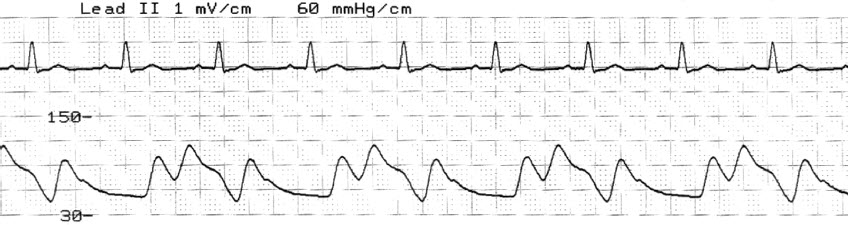
\includegraphics[width=.7\textwidth,height=\textheight,keepaspectratio]{./images/Image00023.jpg}
 \captionsetup{justification=centering}
 \caption{透明隔囊肿\\{\small 透明隔区囊状水样密度灶,囊壁向两侧突出,宽达12mm}}
 \label{fig2-7}
  \end{figure} 



\subsection{侧脑室黏合}

侧脑室不对称在正常人中常见,部分原因是侧脑室黏合,侧脑室黏合是正常变异。

\textbf{【病理】}
本症是在生长发育过程中侧脑室内面部分融合,造成侧脑室不对称、变形。发生在胎儿期4~6周,此时脑白质发育迅速,白质膨大可使邻近的室管膜表面挤压在一起。黏合多发生在额角上侧面及体部,单侧或双侧性。

\textbf{【CT表现】}
侧脑室黏合可以是单侧性或双侧性,或与透明隔间腔同时存在。额角的前部融合,致额角前部消失,额角变短,两壁夹角为锐角,使两壁相交处圆钝的正常表现消失,透明间隔居中。额角中部的两壁尖角状突起,中部间隙消失或接近消失,透明隔居中。透明隔移向一侧,偏移程度从轻度到非常明显,致同侧侧脑室体部变小,对侧相对增大。透明隔的移位必然伴有体部变小侧的额角变窄、变形,但透明隔始终呈直线状走行。双侧基底节区形态结构对称,脑室、脑实质内无异常,增强扫描无异常强化。

\subsection{脑裂畸形}

\textbf{【病因病理】}
有学者认为,妊娠第2个月出现的病理干扰可造成脑壁某部位生发基质层不能正常发育,致使神经元移行不能发生或过早停下来而导致脑裂畸形。其主要病理改变为大脑半球内有自脑表面向内延伸达室管膜下的横行裂隙,邻近皮层卷入衬于裂隙两侧,其表面的软脑膜与室管膜融合形成软脑膜-室管膜缝。脑裂畸形可分为闭合型和分离型两型,常合并透明隔缺如、胼胝体发育不良及其他神经元移行异常等畸形。

\textbf{【临床表现】} 主要有癫痫、智力低下和运动功能障碍。

\textbf{【CT表现】}
大脑半球表面有单侧或两侧的裂隙,从脑表面延伸到室管膜下区。脑皮质沿裂隙内折,居裂隙两侧,多位于中央前后回附近。根据其表现可分为两型:①Ⅰ型:即融合型(或称闭唇型)脑裂畸形,裂隙关闭不与侧脑室相通,但脑室壁可有憩室样突起(图\ref{fig2-8});②Ⅱ型:即分离型(或称开唇型)脑裂畸形,特点为内折的皮质分离,形成较大裂隙并多与侧脑室相通,且脑室壁在内压作用下外突,形成憩室。

\textbf{【鉴别诊断】}
①脑穿通畸形:为大脑成形后的损害(坏死腔),多呈圆形,无脑皮质沿囊肿壁内折为鉴别要点。有时鉴别困难,但穿通畸形的两缘向病灶外方突出,而分离型脑裂畸形两缘向内突出有助于鉴别。②孤立性灰质异位:当融合型裂隙不明显时应注意与其鉴别。脑裂畸形皮质柱内端相邻的侧脑室外壁常有憩室状突起,外端脑表面有楔形凹痕,可与其相鉴别。

\subsection{多微脑回畸形和鹅卵石样脑回畸形}

\subsubsection{无脑回}

大脑皮质表面光滑、无沟回,故又称光滑脑。灰质增厚,白质变薄,灰白质正常手指样交界消失,也可与巨脑回相伴发。

\subsubsection{巨脑回}

局限性或弥漫性脑回异常增宽,皱褶减少,表现为宽、平、厚的脑回,灰白质正常手指样交界亦可消失(图\ref{fig2-8},图\ref{fig2-9})。

\begin{figure}[!htbp]
 {\centering
 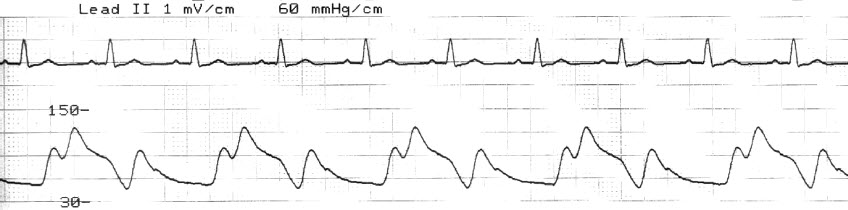
\includegraphics[width=.7\textwidth,height=\textheight,keepaspectratio]{./images/Image00024.jpg}
 \captionsetup{justification=centering}
 \caption{脑裂畸形、双侧额叶巨脑回\\{\small  A、B为同一患者,大脑半球表面两侧均有裂隙,脑皮质沿裂隙内折,位于裂隙两侧,裂隙关闭不与侧脑室相通,灰质相应内移,双侧额叶巨脑回}}
 \label{fig2-8}}
  \end{figure} 



\begin{figure}[!htbp]
 {\centering
 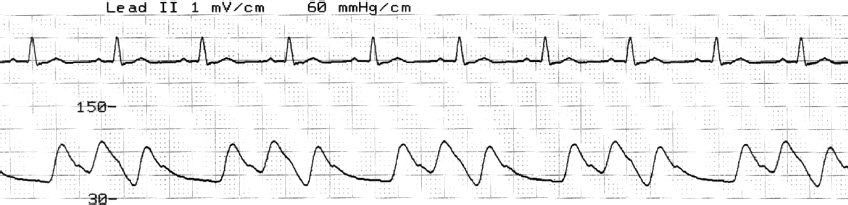
\includegraphics[width=.7\textwidth,height=\textheight,keepaspectratio]{./images/Image00025.jpg}
 \captionsetup{justification=centering}
 \caption{巨脑回}
 \label{fig2-9}}

 右侧额、顶叶脑回弥漫性异常增宽,皱褶减少
  \end{figure} 



\subsubsection{多微脑回畸形}

亦称多小脑回畸形(但该名称易与小脑病变混淆),脑回小且数目增多。

\subsubsection{鹅卵石样脑回畸形}

为复杂的脑畸形,包括鹅卵石样皮质、白质异常、脑室扩大,及脑干、小脑变小并伴有小脑的多微脑回。皮质的异常为无脑回、巨脑回和多微脑回的混合。

\subsection{灰质异位}

本病为灰质在异常部位的聚集。

\textbf{【病因病理】}
原因不明,可能与遗传性、血管性、感染性、环境因素(中毒、辐射、胎儿酒精综合征等)等有关。病理上根据异位灰质灶是否与室管膜相连分为室管膜下型和非室管膜下型,根据病变范围又可分为局灶性和弥漫性。弥漫性90%为女性,往往具有家族史。本病还可伴有其他畸形。

\textbf{【临床表现】}
单纯的灰质异位预后好,可无症状或仅有癫痫。病灶较大或同时伴有其他畸形可表现为中度或严重发育延迟、偏瘫伴癫痫。

\textbf{【CT表现】}
白质内有与灰质密度相等的异常影,增强扫描密度与灰质一致。本病有多种分型方法,通常可分为以下3型。①结节型:呈结节状分布于侧脑室旁,并可突向脑室。②板层型:不规则分布于白质内。③带状型:呈带状分布于白质或皮层下(是最严重的类型,常伴有难治性癫痫,预后相对差)。前两型可单发或多发、单侧或双侧,灰质结节直径1~30mm,无水肿和占位效应。带状型多分布对称,且表面脑回多正常,故较难分辨,易漏诊。

\subsection{脑大畸形}

本病又称头大畸形、巨脑症,为先天性大脑皮质增厚及神经胶质细胞增生。

\textbf{【病因病理】}
本病病因不明,可与遗传因素有关。有学者认为包括体积过大和质量过重两种情况,并将它分为解剖型和代谢型巨脑症。解剖型指细胞体积或数目大于正常,可伴软骨发育不全、神经纤维瘤病、结节性硬化和Chiari畸形等。代谢型是指异常代谢产物积蓄致脑细胞增大,部分伴白质发育不良。本病出生时脑重即可达1600g,或生后头颅迅速增大,皮质和髓质均增厚,可有髓鞘形成不良,无脑积水。

\textbf{【临床表现】}
儿童期发病,常有癫痫和智能低下。头颅周径增大,似先天性脑积水,但无眼球下斜征象(落日征),常有视、听力障碍。

\textbf{【CT表现】}
头颅和颅腔明显增大,大脑皮质增厚,但脑组织密度正常。脑室正常或轻度扩大,脑沟、池正常,中线结构居中。前囟较大、闭合延迟,颅板较薄。

\textbf{【鉴别诊断】}
应注意与继发性巨脑症(如较弥漫的肿瘤、结节性硬化、海绵状硬化及脑积水)、单侧巨脑畸形相鉴别。

\subsection{脑小畸形}

本病又称小脑症、小头畸形或脑小症,发病率为2.5/10万。

\textbf{【病因病理】}
病因不明,可包括先天性遗传因素和胎儿期、新生儿期的各种致病因素如感染、出血、缺氧、产伤等。病理表现为脑小,重量为正常的1/4~1/3,并且脑回结构简单,皮质发育不全,神经元数目减少、排列不整齐,颅骨和颅腔发育小,可合并其他脑发育畸形。

\textbf{【临床表现】}
常表现智能低下甚至呈白痴,也可合并癫痫、运动功能障碍等,出生时头小、外形特殊。

\textbf{【CT表现】}
轻度者可无阳性表现,病变明显时脑室系统和蛛网膜下腔可扩大,皮质光滑,缺乏脑沟、回。严重者可合并胼胝体发育不全、透明隔发育异常、穿通畸形等。颅腔缩小以额部明显,颅板较厚,板障增宽,内板平坦光滑。

\textbf{【鉴别诊断】}
狭颅畸形是颅缝过早闭合限制了脑的发育所致。颅腔常有变形,颅骨脑回压迹增多,且脑室、脑沟、脑池及脑实质常无明显异常,不难与脑小畸形鉴别。此外,一侧大脑半球发育不全与脑小畸形病因病理一样,临床和CT表现相近,不难诊断和鉴别。

\subsection{积水型无脑畸形}

本病是一组少见的先天性前脑畸形,见于婴幼儿,发生率新生儿中占0.2%左右。

\textbf{【病因病理】}
可能与胚胎期脑供血障碍有关,也有人认为是全脑穿通畸形。主要病理改变为双侧大脑半球的额、顶、颞叶完全或大部分缺如,由充满脑脊液的囊性区域取代,其内衬由软脑膜构成(不含室管膜)。基底节、丘脑、中脑可部分或大部分破坏,小脑、桥脑、延髓可发育正常或畸形,脑室系统偶可保存完好,脑膜正常存在,颅骨颅腔大小形态正常或增大。

\textbf{【临床表现】}
头围逐渐增大,多智力低下,可有眼球不规则运动、眼落日征,以及肌张力高、腱反射亢进、抽搐或惊厥、运动机能障碍等。

\textbf{【CT表现】}
幕上双侧大脑半球、脑室大部分缺失,整个颅腔大部分呈脑脊液密度。仅于脑底部见残存的部分枕、额或(和)颞叶组织,基底节、丘脑部分存在,大脑镰完整存在。幕下结构正常,但脑干可略变细。

\textbf{【鉴别诊断】}
有学者把极其严重的双侧性开唇型脑裂畸形归类于积水性无脑畸形中,影像学二者难以鉴别,但后者还能识别脑室轮廓,特别是前角的下部和后角。还应注意与无脑叶型前脑无裂畸形、穿通畸形、巨大蛛网膜囊肿及重度脑积水鉴别。

\subsection{脑穿通畸形}

本病是在脑组织分化发育充分之后,由于各种原因造成的脑组织破坏缺损,并与蛛网膜下腔或脑室相通。

\textbf{【病因病理】}
有先天性和获得性之分。先天性病因不明,可能与胎儿期血管闭塞或发育畸形有关;获得性是由于外伤、感染、缺氧、血管疾病引起正常脑组织坏死液化。缺损边缘为胶质瘢痕,不含神经细胞。

\textbf{【临床表现】} 依病变范围而定,可表现运动障碍、癫痫等。

\textbf{【CT表现】}
脑实质内巨大的脑脊液密度样囊肿,界限清楚,增强扫描无强化。与脑室或(和)蛛网膜下腔相通是诊断的关键,同侧侧脑室一般相应扩大。

\subsection{先天性中脑导水管狭窄}

本病亦属脑的发育畸形。

\textbf{【病理】}
狭窄多位于导水管口以下3~4mm处。狭窄的形态多样,可呈线状、鸟嘴状、漏斗状、隔膜状或分叉状,狭窄以上脑室积水。

\textbf{【临床表现】} 临床症状常开始于幼儿,呈慢性脑积水表现。

\textbf{【CT表现】}
侧脑室及第三脑室对称性扩大,第四脑室正常或略小。侧脑室周围有带状低密度区,代表阻塞性脑积水的典型表现。重度积水患者,可表现幕上大脑半球区为水样低密度,额、顶、颞叶脑实质几乎消失或残留极少,部分枕叶、基底核和丘脑保存,小脑和脑干发育一般正常,第四脑室位置、形态正常,可见正常大脑镰结构(图\ref{fig2-10}),MR可显示狭窄的形态。

\begin{figure}[!htbp]
 {\centering
 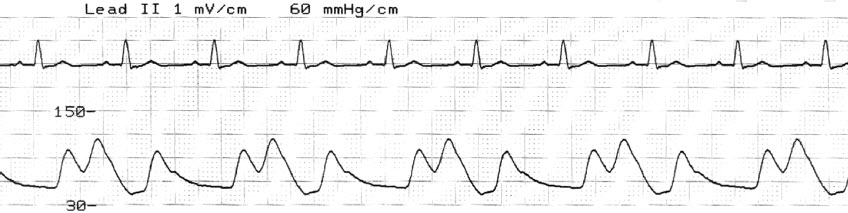
\includegraphics[width=.7\textwidth,height=\textheight,keepaspectratio]{./images/Image00026.jpg}
 \captionsetup{justification=centering}
 \caption{先天性中脑导水管狭窄\\{\small  A、B为同一患者,可见第三脑室、侧脑室积水扩张,额、顶、颞叶脑实质部分残留,枕叶、部分基底核和丘脑保存,小脑和脑干发育正常,第四脑室正常}}
 \label{fig2-10}}
  \end{figure} 



\textbf{【鉴别诊断】}
应注意与松果体区和中脑肿瘤压迫所致的导水管狭窄相鉴别,但肿瘤有占位表现且导水管有移位。炎性粘连所致的导水管狭窄与本病不易鉴别。此外,积水性无脑畸形大脑结构几乎完全消失、脑室基本无残留,枕叶一般相对完整,可予鉴别。

\subsection{结节性硬化症}

本病又称为Bourneville病,是一种较少见的常染色体显性遗传病,发病率约为1/50000~2/10000。

\textbf{【病理】}
病理特征为皮质结节、白质内异位细胞团和脑室内的小结节。结节可发生于皮质、室管膜下,皮质结节最常位于额叶,其次枕叶,偶见于基底节、丘脑、小脑和脑干。皮质结节内含有细胶原纤维、奇异的胶质细胞或不典型的神经元,多数有钙化。脑白质内异位细胞团也是由胶质细胞和神经节细胞组成。室管膜下结节最易钙化,易伴发室管膜下巨细胞型星形细胞瘤,也可伴有视网膜的错构瘤及其他内脏肿瘤。皮质腺瘤由皮质腺、结缔组织和血管组成,但国外有学者认为面部多发的不是皮脂腺瘤,无皮脂腺样结构,而是血管纤维瘤。

\textbf{【临床表现】}
典型的三联征为:①皮质腺瘤占90%;②癫痫发作;③智力低下。但三者不一定同时出现。皮质腺瘤主要位于面颊、鼻、额或两耳处,为对称散发、针头大小、黄红色透亮的坚硬蜡状丘疹。本病还可有眼、心、肾、肺、骨骼病变。

\textbf{【CT表现】}
有以下几方面:①皮质结节:可见脑回扩大、增宽,结节呈低密度,周围为等密度厚皮质围绕。一般无强化,故有人称为空心型病灶。此外,还可呈“H”型皮质结节(低密度病灶中间有一等密度横道)和高密度团块。②室管膜下结节:位于脑室边缘,50%以上双侧对称多发,结节大小不等,部分钙化,未钙化部分强化著(图\ref{fig2-11})。③室管膜下区星形细胞瘤:常位于室间孔附近。④脑白质内异位的细胞丛:皮髓交界区或更广泛的白质内见一些更低密度区。⑤其他:可有脑沟增宽等脑萎缩表现;阻塞室间孔可有脑积水表现。

\begin{figure}[!htbp]
 \centering
 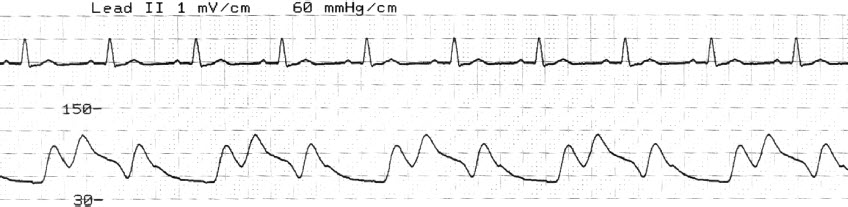
\includegraphics[width=.7\textwidth,height=\textheight,keepaspectratio]{./images/Image00027.jpg}
 \captionsetup{justification=centering}
 \caption{结节性硬化症\\ {\small 左右侧侧脑室边缘可见多个钙化结节,大小不等;右侧额叶有局限性萎缩表现}}
 \label{fig2-11}
  \end{figure} 



\subsection{脑颜面血管瘤病}

本病又称Sturge-Weber综合征或软脑膜血管瘤病。

\textbf{【病因病理】}
此病多为散发,很少有家族遗传史,偶为常染色体显性遗传。病变的分布特点为面部三叉神经分布区皮肤毛细血管瘤和同侧颅内软脑膜血管瘤,病侧大脑发育不良或萎缩。由于软脑膜血管瘤长期压迫或继发性脑缺血可引起皮质梗死,神经节细胞减少、变性,神经胶质增生伴皮质钙化,30%可发生青光眼与脉络膜血管瘤。

\textbf{【临床表现】}
癫痫、痴呆、智力低下,轻偏瘫、偏盲,先天性青光眼、牛眼症(先天性白瞳症)等,还可合并阴睾、脊柱裂等。面部分布葡萄酒色的血管痣,称作火焰痣或葡萄酒斑,出生时即可存在,主要分布在一侧三叉神经分布区,一般同颅内软脑膜血管瘤位于同一侧,但少数也可位于双侧或对侧面部。此外,约5%~15%的患者无面部血管痣。

\textbf{【CT表现】}
患侧皮层曲线状或脑回状钙化为本病特征(图\ref{fig2-12})。患侧大脑皮质萎缩伴脑沟裂、脑池增宽增深及同侧脑室扩张,钙化周围可见梗死灶,偶见出血灶。同侧脑室脉络丛有时增大,颅盖骨板障可增厚。增强扫描钙化灶周围及钙化区可明显强化;增大的脉络丛(亦属血管瘤)有明显强化。在发现脑实质内的缺血缺氧、胶质增生和脱髓鞘改变方面CT不及MR。

\begin{figure}[!htbp]
 \centering
 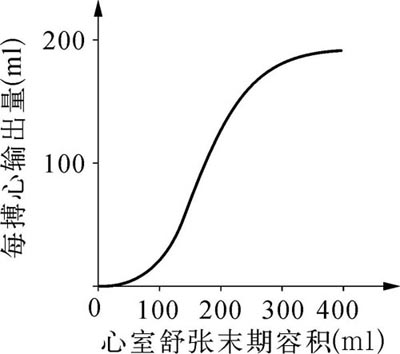
\includegraphics[width=.7\textwidth,height=\textheight,keepaspectratio]{./images/Image00028.jpg}
 \captionsetup{justification=centering}
 \caption{Sturge-Weber综合征\\{\small 右侧额叶皮层曲线状钙化,局部脑沟增宽增深}}
 \label{fig2-12}
  \end{figure} 



\textbf{【鉴别诊断】}
颅内类似的脑回状钙化也可见于胶质瘤、脑梗死、化脓性脑膜炎、骨化性脑膜脑病,故应结合本病的其他征象及临床特征予以鉴别。

\subsection{共济失调性毛细血管扩张症}

本病又称Louis-Bar综合征,是一种常染色体隐性遗传性疾病,发病率约1/40000,主要发生在儿童,男女发病相近。

\textbf{【病理】}
主要病理改变是小脑皮质萎缩,尤以蚓部为甚,齿状核-橄榄体退变、脑干中的轴索肿胀。小脑血管异常可能是其病因。

\textbf{【临床表现】}
主要特征是小脑机能障碍(共济失调),进行性眼皮(可涉及眼结膜)毛细血管扩张。患儿易患鼻窦炎、肺部感染,以及淋巴系统肿瘤。

\textbf{【CT表现】}
主要表现为以蚓部为主的小脑萎缩。小脑沟增宽增深、数目增多,小脑下蚓发育不良,四脑室扩张,小脑周围蛛网膜下腔、脑池增宽。如伴脑实质毛细血管扩张破裂,可出现脑出血。有时可见脑梗死,由来自肺内血管畸形的栓子所致。

\subsection{神经纤维瘤病}

本病是中胚层和神经外胚层的常染色体显性遗传病。

\textbf{【病理】}
主要是神经外胚层结构的过度滋生、中胚层异常发育及多发性肿瘤形成,可累及全身各系统和器官。有学者将本病分为以下5型。Ⅰ型:为局限性神经纤维瘤病,以丛状神经瘤为特征;Ⅱ型:为全身性皮肤神经纤维瘤病,以多发性皮肤结节及皮肤色素斑为主要表现;Ⅲ型:为深部周围神经干的神经瘤、神经纤维瘤和神经鞘瘤,以深部神经干过分受累为特征;Ⅳ型:为颅神经干的神经瘤、神经纤维瘤、神经鞘瘤,以双侧听神经瘤为多见;Ⅴ型:为并发脑瘤和脑瘤样变,可合并脑膜瘤、胶质瘤、血管瘤、黑色素瘤、结节性硬化、脊髓空洞症、播散性胶质结节增生等。其中Ⅰ型最常见,约1/1000神经纤维瘤可恶变。

颅内最常见的肿瘤有听神经瘤(多为双侧)、视神经胶质瘤、三叉神经瘤、基底节和丘脑部胶质瘤及多发性脑膜瘤等。此外,还可有脊神经根或马尾的神经纤维瘤、脊膜瘤,颅骨和脊柱发育异常也较常见。

\textbf{【临床表现】}
本病可见于任何年龄,但在10~20岁和50~70岁有两个发病高峰期,男多于女。其临床特点是皮肤可见特征性棕色斑(奶油咖啡色素斑)伴皮肤软组织肿块以及各组织的肿瘤形成,可有轻度思维障碍和癫痫。约1/2病例有骨骼改变(系中胚叶发育障碍和神经纤维瘤侵蚀所致),还可并发甲状旁腺功能亢进和肢端肥大症。

\textbf{【诊断标准】}
美国国立卫生研究院的诊断标准如下:①体表至少有5个直径>5mm的咖啡斑;如果是青春前期,则应有6个以上且直径>15mm;②临床或组织学证实有2个以上的神经纤维瘤或丛状神经纤维瘤;③在腋窝或腹股沟部出现多发性雀斑;④蝶骨翼结构不良或伴有骨发育畸形;⑤双侧视神经的神经胶质瘤;⑥裂隙灯检查示虹膜有2个或更多的Lish结节;⑦患者一级亲属中患有本病。具备其中两条或两条以上即可诊断为本病。

\textbf{【CT表现】}
颅内肿瘤常见的是听神经瘤,其次为三叉神经和颈静脉孔区神经纤维瘤;脑膜瘤约半数多发;偶并发胶质瘤,可发生于视交叉、脑干与基底核处。脑发育异常可有脑大畸形、胼胝体发育不全、Chiari畸形、巨脑回畸形、灰质异位等。脑血管异常有动脉瘤、动静脉畸形和动静脉瘘等。眶内肿瘤可为视神经纤维瘤、脑膜瘤或胶质瘤。脊髓肿瘤可以是马尾神经纤维瘤、脊膜瘤或室管膜瘤。

\subsection{小儿21-三体综合征}

本病又称先天愚型、Down综合征,是常见的染色体异常疾病,21号染色体三体是生殖细胞在减数分离过程中,发生不分离所致。

\textbf{【病因病理】}
与母亲妊娠时的年龄(年龄越大发病率越高)、遗传因素、妊娠时化学药物堕胎、放射线、自身免疫性疾病有关。本病主要病理变化为中枢神经系统发育异常。患儿染色体核型为47,XX(XY),+21,双亲核型正常。

\textbf{【临床表现】}
患儿表现在出生时就很显著,有的体征到1岁时才明显。根据其特殊的愚型面容、皮纹特征和智能落后容易诊断。

\textbf{【CT表现】}
①脑内钙化:多见于基底节区,呈点状或小圆形;②大脑发育不良:侧裂、额顶区蛛网膜下腔增宽;③小脑发育不良:轻度对称性小脑发育不良常见于本病;④脑干可变小,桥小脑角池、枕大池相应增大;⑤
<1岁的婴儿CT可表现正常,可能与病程演变有关。

\textbf{【鉴别诊断】}
本病应注意与结节性硬化、甲状旁腺功能减退(图\ref{fig2-13})、弓形体病、Fahr病相鉴别。

\begin{figure}[!htbp]
 {\centering
 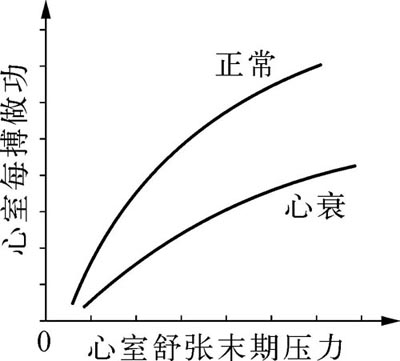
\includegraphics[width=.7\textwidth,height=\textheight,keepaspectratio]{./images/Image00029.jpg}
 \captionsetup{justification=centering}
 \caption{甲状旁腺功能减退\\{\small  A、B为同一患者,男14岁,左右侧基底核、左右侧丘脑、皮髓质交界处广泛对称性钙化}}
 \label{fig2-13}}
  \end{figure} 



\section{新生儿及婴幼儿脑疾病}

\subsection{正常新生儿和早产儿脑的CT特点}

\subsubsection{正常新生儿的脑CT表现}

1.白质密度较低:与新生儿脑组织水分含量多(且与胎龄成反比)有关。正常新生儿的脑白质密度为18~28Hu(平均>21Hu),脑灰质为26~39Hu(平均31Hu)。

2.灰白质分界模糊:人脑传导系统从胎龄7个月开始发育,神经纤维逐渐从白质伸向灰质,但出生时为数尚少,且髓鞘形成尚不完全;同时小儿脑富含蛋白质,而脂类含量少,故灰白质交界缺乏密度差异。

3.硬膜窦密度高:与窦内血流缓慢、血容量大、富含红细胞和血红蛋白等有关。

4.基底部脑池和第四脑室宽大:是因胎儿及新生儿大脑发育优于小脑和脑干所致,故桥前池和桥小脑角池亦显示较宽,纵裂池相对较窄。

5.透明隔间腔:8个月以前胎儿全部存在,新生儿82%存在,随年龄增长发生率下降。2~5周岁时为5%~6%,5~9周岁时为2.7%,10~14周岁为2.3%。

\subsubsection{早产儿的脑CT表现}

早产儿脑发育不成熟,脑组织含水量高,脑髓质化不完全,缺乏髓鞘形成,在颅脑CT扫描时可存在较广泛的或弥漫性白质低密度区,皮层灰质较薄,密度相对较高(图\ref{fig2-14}B),灰白质分界清楚,且与颅骨、脑室间形成良好的对比。

\subsection{新生儿缺氧缺血性脑病}

本病是围产期缺氧引起的脑部损害,在小儿CT检查中占7.2%,在新生儿CT检查中占94%,甚至有报道达94%~100%。

\textbf{【病因病理】}
主要病因是窒息,由宫内窒息引起的占50%,娩出过程窒息的占40%,其余10%由生后肺部疾病、呼吸暂停、红细胞增多症、败血症、先心病等所致。缺氧导致细胞内水肿、血管源性水肿,进而发生脑坏死,并由于血管通透性增加和脑血管调节失调、静脉压升高而发生颅内出血。

\textbf{【临床表现】}
可分为3度:①轻度:表现兴奋、易激惹、肢体颤动、肌张力高、反射活跃,症状于1天内好转。②中度:嗜睡、反应迟钝、肌张力低、反射减弱、惊厥、呼吸不规则,症状于1周内消失,可有后遗症。③重度:神志不清、肌张力松软、反射消失、反复发生惊厥、呼吸不规整、瞳孔不对称、对光反应消失,常在1周内死亡,存活者可有脑瘫、脑积水、智力低下、癫痫等后遗症。

\textbf{【CT表现】}
主要为脑水肿、颅内出血及脑组织坏死。①脑水肿:是早期重要征象,脑实质密度(主要是白质密度)减低,CT值≤18Hu,好发于额、顶叶。前囟隆起、颅缝增宽,脑沟、回浅扁且脑室变窄,脑室、脑池受压(图\ref{fig2-14}A)。②颅内出血:多为蛛网膜下腔出血,但脑外伤亦可致蛛网膜下腔、硬膜下、脑室内或脑室周围出血。③脑组织坏死:早产儿脑组织坏死好发于室旁白质又称为室旁白质软化,也可液化形成软化灶。

\begin{figure}[!htbp]
 {\centering
 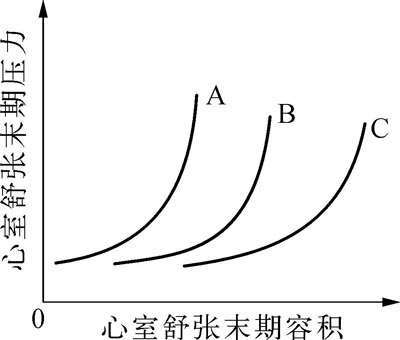
\includegraphics[width=.7\textwidth,height=\textheight,keepaspectratio]{./images/Image00030.jpg}
 \captionsetup{justification=centering}
 \caption{新生儿缺氧缺血性脑病\\{\small  A.左右额、顶叶白质区云絮状低密度灶,CT值约14~16Hu;B.皮层灰质薄,密度相对较高,灰白质分界欠清楚}}
 \label{fig2-14}}
  \end{figure} 



\textbf{【CT分度】}
①轻度:脑实质低密度影分布于1~2个脑叶,少数合并少量颅内出血(多为蛛网膜下腔出血)。②中度:低密度影超过2个脑叶,灰白质界限模糊,部分脑沟消失,约1/3合并颅内出血。③重度:弥漫性低密度影,灰白质界限消失。基底节、丘脑密度正常,脑室受压变窄,并发颅内出血者约占80%。

但我们认为对于超过2个脑叶者,如位于各叶的病灶面积均较小,且灰白质界限较清晰者,应诊断为轻度,以便于与临床分度相对应。

\textbf{【并发症】}
①轻度者于1~2个月病变多吸收,无明显后遗症。②中度者大多数亦可治愈,少数可出现外部性脑积水、脑发育不良、脑萎缩等。③重度者约35%于1周内死亡,存活者多有后遗症如脑萎缩、脑皮质变薄、脑白质减少、脑白质变性、脑软化、脑穿通畸形、钙化等。有报道病变处CT值<12Hu的重度患者多有并发症。

\textbf{【鉴别诊断】}
早产儿脑CT表现为较广泛的或弥漫性白质低密度区;皮层变薄、密度相对增高,呈花环状改变;灰白质分界清楚,脑室系统未见异常,中线结构无移位。早产儿缺氧性脑损伤灰白质界限模糊(图\ref{fig2-14}B),有颅内出血和脑室旁出血性脑梗死、脑室周围白质和脑白质发育不良及脑梗死等。两者CT表现有所区别,但早产儿合并缺氧性脑损伤时,CT难以分级。

\subsection{新生儿颅内出血}

本病是新生儿常见的急症,为新生儿死亡和以后神经发育障碍的主要原因之一。

\textbf{【病因病理】}
病因主要有新生儿缺氧缺血性脑病、产伤、早产,少数为出血性疾病、颅内先天性血管畸形。①缺氧使脑组织充血、水肿、脑血管壁通透性增高,引起渗血或点状出血;同时缺氧可使肝脏合成凝血因子发生障碍,从而加重出血。②产伤可造成硬膜窦撕裂或皮质桥静脉、脑内的静脉以及脉络丛静脉破裂。出血常见部位为硬膜下,其次为蛛网膜下腔,也可发生于脑实质、脑室内或硬膜外。③原发性出血性疾病、颅内先天性血管畸形引起的出血很少见,前者多位于蛛网膜下腔,后者可在蛛网膜下腔或脑实质内。

\textbf{【临床表现】}
少量出血时可无症状,量多时可出现激惹、尖叫、惊厥、烦躁不安、呕吐等症状,2天后出现抑制症状如嗜睡、拒奶、昏迷、四肢张力低下及呼吸不规则、青紫等。

\textbf{【CT表现】}

1.硬膜下出血:多见于足月儿,常有头皮血肿、颅骨骨折、颅缝分离。

2.蛛网膜下腔出血:最常见,有3个特征性征象。①空三角征:又称矢状窦旁征,血液积聚于矢状窦旁呈高密度,静脉窦内流动的血液呈相对低密度,底边为颅骨,形成空心形△征象。②高脚杯征:又称天幕缘征,即血液沉积于小脑幕缘上下形成“Y”或“V”形高密度影。③纵裂池边缘模糊征:即纵裂池内出血高密度影边缘模糊。以上3个征象的出现率可达50%~80%(图\ref{fig2-15})。此外,有学者认为“直窦”宽>5mm可认为有出血。

\begin{figure}[!htbp]
 {\centering
 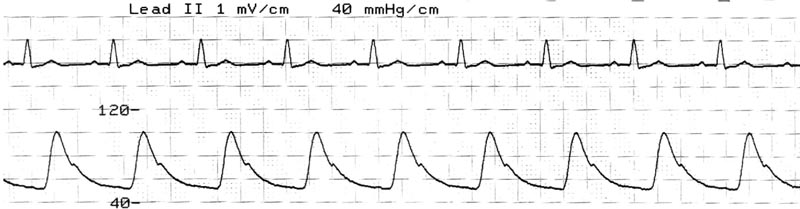
\includegraphics[width=.7\textwidth,height=\textheight,keepaspectratio]{./images/Image00031.jpg}
 \captionsetup{justification=centering}
 \caption{新生儿蛛网膜下腔出血\\{\small  A.高脚杯征;B.空三角征,伴有脑室内出血;C.纵裂池边缘模糊征}}
 \label{fig2-15}}
  \end{figure} 



3.脑实质内出血:呈点状或斑片状高密度灶,有或无水肿带。

4.室管膜下及脑室内出血:常见于早产儿。因室管膜下胚胎生发层组织发育不成熟,血液极易渗出,多量渗出可破入侧脑室,并可致脑积水。

5.其他:包括硬膜外出血和小脑出血,均较少见。

\textbf{【鉴别诊断】}
①钙化:新生儿颅内出血CT值为50~80Hu,新生儿颅内钙化少见且均为病理性,CT值>80Hu,因此不难鉴别。②晚发性维生素K缺乏症:发病年龄多在1~2个月小婴儿,出血量大、部位多,常有血团块形成、液平面出现及伴有脑梗死、大面积水肿,可予鉴别。

\subsection{婴儿维生素K缺乏症}

本病又称迟发性维生素K缺乏症、晚发性维生素K缺乏症,是指新生儿晚期(出生后2周)至乳儿期,因缺乏维生素K而引起的出血性疾病。

\textbf{【病因病理】}
常见的原因有3种:①维生素K摄入不足;②合成障碍;③吸收不良。维生素K是合成多种凝血因子所必需的辅酶,缺乏凝血因子凝血活性丧失,造成自发出血。

\textbf{【临床表现】}
发热、惊厥抽搐、呕吐、烦躁不安、拒乳、嗜睡等;可伴皮肤、消化道、上呼吸道出血等,并出现相应表现。婴儿期特别是1~4个月内母乳喂养儿若出现进行性贫血、全身出血倾向并伴急性颅内高压等精神症状应首先考虑本病。实验室凝血时间、凝血酶原时间延长及部分凝血活酶原时间延长可肯定诊断。

\textbf{【CT表现】}
①颅内出血:特点为出血量大,多发部位出血(脑实质内、外或脑室等);②脑水肿、脑梗死:是由于血管受挤压或痉挛所致,可呈广泛小片状水肿表现或大面积梗死,甚至半球缺血性改变;③脑疝;④一侧侧脑室闭塞,对侧侧脑室扩张积水;⑤并发症:存活者可致外部性脑积水、脑软化、脑萎缩、脑穿通畸形或脑发育不良。

\subsection{新生儿胆红素脑病}

持久性或明显的新生儿高胆红素血症可以导致脑部损伤。

\textbf{【病因病理】}
最常见的原因是红细胞溶血,其他原因包括红细胞增多症、胆红素结合方面的遗传或获得性缺陷、消化道运转方面的疾患及激素的紊乱等。未结合胆红素进入脑组织,结合于脑细胞膜,抑制细胞线粒体酶的活性,使脑细胞能量代谢障碍,致脑部损伤。

\textbf{【临床表现】}
足月儿常在生后2~5天,早产儿常在7天左右发生本病。典型的临床表现分为4期:①警告期;②痉挛期;③恢复期;④后遗症期。

\textbf{【CT表现】}
尚无报道本病有特异性CT表现。MR在急性期呈短T1和长T2信号;慢性期苍白球、下丘脑和海马显示长T2信号。

\subsection{血钠过高性脱水}

\textbf{【病因病理】}
最常见的原因是严重的腹泻,钠在细胞间隙中浓度升高致细胞内液体减少并皱缩。脑离开颅板导致桥静脉撕裂,另外血液的高渗致毛细血管增粗,易发生毛细血管破裂及脑实质出血。

\textbf{【临床表现】}
年幼儿童,尤其是未成熟儿对血钠过高有易感性。病儿极度冷漠、对刺激易激性高,另外还有肌肉强直、反射亢进,偶有癫痫。

\textbf{【CT表现】}
间质水肿引起脑实质密度降低,在大脑和小脑灰白质交界处可见高密度出血灶。

\subsection{新生儿低血糖症}

低血糖的标准是足月儿血糖低于16.7mmol/L(300mg/L),未成熟儿低于11mmol/L(200mg/L)。大多数低血糖的新生儿发病早,持续时间短,对葡萄糖反应迅速。但足月小样儿在子宫内就遭受营养不良,大多有临床症状,低血糖程度相对较重,持续时间可以延长,治疗需大量的葡萄糖。引起脑损害最通常的原因是继发于胰腺β细胞的先天性肿瘤或增生性胰岛素分泌过多。

\textbf{【CT表现】}
围产期低血糖脑损害表现为:①急性期:皮质和皮质下白质的脑水肿,以顶枕部最重;②慢性期:皮质和皮质下白质萎缩。

\subsection{外部性脑积水}

本病亦称良性蛛网膜下腔增宽,是一种特殊的交通性脑积水。一般2岁内自愈。

\textbf{【病因病理】}
有新生儿缺氧缺血性脑病、出血、外伤、感染等,半数病因不明为特发性。其发病机制可能为蛛网膜颗粒对脑脊液的吸收障碍所致。多数学者认为颅缝开放是其发生的前提。

\textbf{【临床表现】}
抽搐(约占50%以上)和头围增大(占1/3~2/3);部分患儿无症状。抽搐的发生与本病的严重程度密切相关。本病好发于2~24月前囟未闭的小儿,但可在生后数天发生,3~6个月为典型期,9个月~1岁开始好转,2岁前或囟门闭合前基本恢复正常。

\textbf{【CT表现】}
额叶或额、顶叶蛛网膜下腔间隙>5mm,而后部不宽。前纵裂池增宽>7mm,后纵裂池不宽。外侧裂池增宽>7mm。鞍上池稍大。额、顶叶脑沟部分增宽,但增深不著。大脑后半部及小脑正常。脑室正常或轻度扩大(图\ref{fig2-16})。

\begin{figure}[!htbp]
 {\centering
 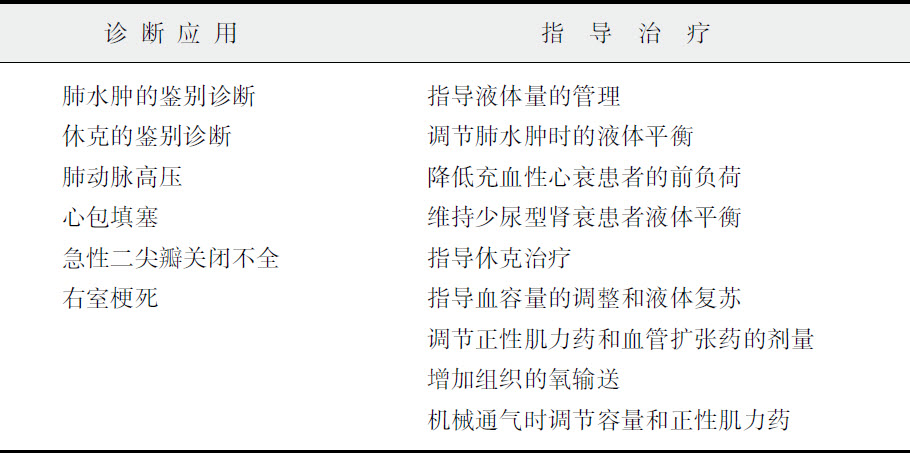
\includegraphics[width=.7\textwidth,height=\textheight,keepaspectratio]{./images/Image00032.jpg}
 \captionsetup{justification=centering}
 \caption{外部性脑积水\\{\small  A、B为同一患者,额、顶叶蛛网膜下腔间隙>5mm,而后部不宽;前纵裂池增宽>7mm,后纵裂池不宽;外侧裂池增宽>7mm}}
 \label{fig2-16}}
  \end{figure} 



总之,本病诊断的依据是:①前囟未闭的婴儿及头颅增大;②脑前部脑外积液增多,脑实质无改变;③2岁后脑外积液自然吸收。

\textbf{【鉴别诊断】}

1.在诊断外部性脑积水时,应除外其他因素引起的蛛网膜下腔增宽,其中包括促肾上腺皮质激素和皮质类固醇的治疗、脱水、营养不良以及癌肿化疗等。

2.脑萎缩:①外部性脑积水头围大,常有抽搐,无智力低下及运动障碍;而脑萎缩头围小,常有智力低下及运动障碍。②前者仅脑的前部蛛网膜下腔增宽;而脑萎缩常全脑蛛网膜下腔及脑沟增深、增宽。③前者纵裂池增宽限于前部;而后者则为整个增宽。④前者脑皮质厚度正常,脑沟可增宽但增深不著;而后者脑皮质变薄,密度减低及脑沟普遍加深。⑤脑室大小不能用于两者的鉴别,因为外部性脑积水可有轻度脑室增大。但脑萎缩时脑室与颅脑横径之比大于正常,而外部性脑积水正常。双额叶局限性脑萎缩时鉴别有一定难度,其双侧额角的局限扩大有助于与外部性脑积水鉴别。

3.硬膜下积液:本病多为单侧,双侧时常不对称,脑沟相互聚拢而不是加深加宽,不难鉴别。

4.脑发育迟缓:多表现为灰白质比例失常,常合并其他多种神经系统畸形。

\subsection{儿童脑室周围白质软化症}

本病又称为脑室周围萎缩、脑室周围白质发育不良,多认为好发于早产儿及产后窒息存活的儿童。

\textbf{【病因病理】}
与缺血缺氧及感染有关,主要损伤轴索及少突胶质细胞,但发病机制尚不清楚。病变主要分布于侧脑室三角区及枕角周围白质、额角附近白质。病理上脑白质由于缺血缺氧发生水肿、凝固、坏死,继而吸收或形成瘢痕和胶质增生,弥漫或局限的胶质损伤使髓鞘化延迟、白质减少,从而导致侧脑室扩张。

\textbf{【临床表现】}
本病可以导致脑瘫(主要是痉挛性下肢瘫或四肢瘫)、智力落后、抽搐,以及各种眼的异常如眼颤、斜视、视力下降等。

\textbf{【CT表现】}
显示脑室周围和半卵圆中心的脑白质明显减少,皮质与脑室缘距离甚小或消失,也可见呈斑片状或长条状的软化灶(图\ref{fig2-17})。一侧或两侧侧脑室扩大,扩大的脑室轮廓不规则可与脑积水鉴别。

\begin{figure}[!htbp]
 \centering
 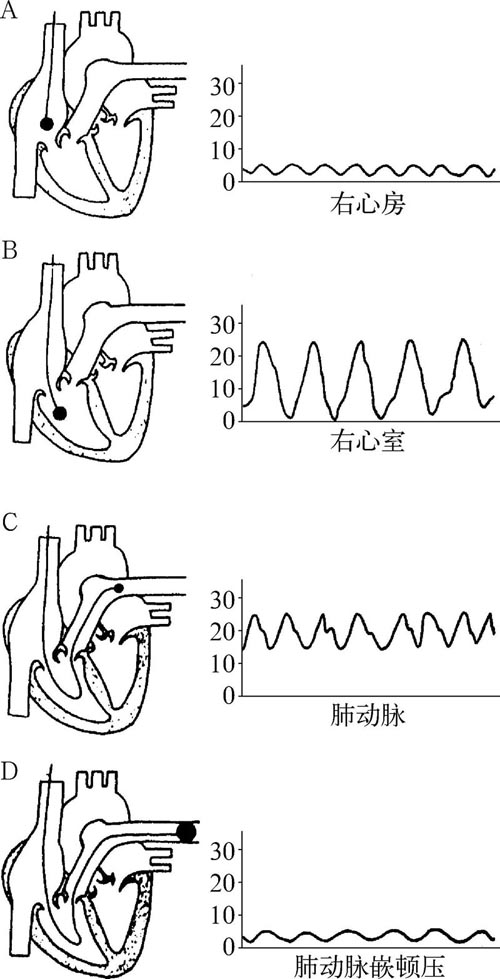
\includegraphics[width=.7\textwidth,height=\textheight,keepaspectratio]{./images/Image00033.jpg}
 \captionsetup{justification=centering}
 \caption{脑室周围白质软化症\\{\small 脑室周围和半卵圆中心的脑白质明显减少(右侧显著),皮质与脑室缘距离甚小,右侧有斑片状软化灶}}
 \label{fig2-17}
  \end{figure} 



\subsection{儿童脑性瘫痪的相关疾病}

本病是指出生前至出生后1个月内各种原因所致的非进行性脑损害综合征。临床表现为中枢性运动障碍及姿势异常,可伴智力低下、癫痫、视力障碍及行为异常。其CT改变可分为以下6种类型。

1.脑发育畸形:可分为器官源性和组织源性(已于上节详述)。

2.脑萎缩:大多由于缺血性损害或颅内感染导致脑白质或灰质减少、丧失,是脑性瘫痪最常见的CT表现。①可表现为脑沟裂增宽、增深,脑室增宽等。②其中脑室周围白质软化(PVL)约占脑萎缩的65%。③小脑萎缩可见小脑上沟增多(3条或3条以上)。

3.脑软化灶:多发生于较成熟的脑组织,可能与新生儿缺氧缺血性损害及颅内出血有关。

4.基底节病变:多由于脑血管阻塞致脑缺血缺氧性损害以及颅内感染、出血或中毒引起苍白球、丘脑区铁钙质沉着及神经细胞变性坏死。CT表现一侧或两侧对称性钙化灶或软化灶。

5.混合型:即上述两种以上病变混合存在。

6.正常:其原因可能为:①CT未能显示全部病灶或遗漏;②少数脑瘫与病变部位神经递质异常有关,CT不能显示;③胎儿期囊性病灶出生后自行消失;④CT检查的局限性,如CT难以显示矢状窦旁区脑损害及髓鞘形成延迟或发育不良。

\section{脑积水}

\subsection{概述}

1.脑积水:是指由于脑积液的产生和吸收不平衡所致的脑室扩大。按其发病机理可分为两大类:①脑脊液循环或吸收障碍;②脑脊液分泌增加。后者非常少见,主要见于脑室肿瘤如脉络丛乳头状瘤。脑脊液的吸收过去认为是通过蛛网膜颗粒,20世纪70年代后认为它不是惟一的吸收途径,并有学者认为主要是通过中枢神经系统表面吸收。

2.交通性脑积水:是指第四脑室出口以下的正常脑脊液通路受阻或吸收障碍所致的脑积水。国外有学者提出交通性脑积水应改称为动脉搏动限制性脑积水。动脉搏动明显减弱可能是由于动脉壁变硬或蛛网膜下腔顺应性降低所致。但动脉压并没有降低且传递的更远,使脑内脉压增高,大脑皮层压力梯度增大,脑室系统扩大。

3.阻塞性脑积水:又叫做非交通性脑积水,是指脑室系统即第四脑室出口以上任何部位发生阻塞所造成的脑积水,是最常见的脑积水。

脑积水时侧脑室旁白质内,CT上可见不规则低密度,是由于间质性水肿所致。即在脑室内压力增高时,室管膜受损出现小裂隙,水分子由此进入侧脑室周围白质内形成间质性水肿。高血压、动脉硬化及部分脑萎缩病人也可在室旁白质内出现上述CT表现(或异常MR信号),但其机理与脑积水不同,可能与局部组织变性、胶质增生、细胞萎缩后间隙扩大等有关。

\subsection{交通性脑积水}

\textbf{【病因】}
主要有蛛网膜下腔出血、脑膜炎、颅脑损伤以及静脉栓塞,亦可见于脑膜瘤病、脑脊液吸收功能障碍等。

\textbf{【临床表现】} 主要表现为颅内压增高的症状和体征。

\textbf{【CT表现】}
典型表现是脑室系统普遍扩大;另一特征是脑沟变浅、变平(但也可正常甚至扩张)。早期为颞角扩大和钝圆,稍后为额角扩大,进一步加重出现第三脑室扩大,第四脑室扩大较晚,与脑萎缩相比第三脑室扩大更明显。但有时交通性脑积水表现不典型,特别合并脑萎缩时,诊断较困难。此外,蛛网膜下腔出血和化脓性脑膜炎可表现为急性脑积水,脑室系统短时间内明显扩大。

交通性脑积水的特征之一为脑沟变浅、变平且灰白质界限清楚,常据此帮助诊断。但有时脑沟、脑池扩大,特别是纵裂池、基底池和桥小脑角池扩大。这种情况多见于基底池等有关脑池的炎症或肿瘤所致的部分脑脊液循环通路受阻及脑脊液吸收障碍。

脑室旁白质水肿发生率约为40%,且长期存在的交通性脑积水往往不出现这种征象。这是因为长期室内高压所致的室管膜受损,发生胶质增生形成室管膜瘢痕,阻止了脑脊液渗漏。

\subsection{正常压力性脑积水}

本病是交通性脑积水的一种特殊类型,多发生在慢性交通性脑积水的基础上,部分完好的脑脊液循环吸收功能代偿,且脑脊液的分泌功能下降,从而形成新的平衡。此时,虽然脑室系统仍明显扩大,但脑脊液压力正常,故又称为常压性脑积水。但实际上,大多并不一直正常,呈波动性。

\textbf{【临床表现】}
一般无颅内高压征,可能由于扩张侧脑室对周围白质的压迫,出现痴呆、步态不稳等症状。

\textbf{【CT表现】}
多不典型。由于脑室内压力正常,可在脑室扩大的同时出现脑沟加深,但两者不呈比例,脑室扩大更著。

\subsection{阻塞性脑积水}

\textbf{【病因病理】}
主要有先天性疾病、感染性疾病和肿瘤。病理表现为脑实质变薄,并可继发脑萎缩、白质脱髓鞘、胶质增生和神经细胞退行性变。

\textbf{【临床表现】}
主要为颅内压增高的症状和体征。其中先天异常、胎儿期或出生过程中发生该病者多在婴幼儿期出现症状,有的至10岁后或成年才表现异常。患儿有头颅增大,两眼球下旋形成“落日征”等甚有特点。

\textbf{【CT表现】}
阻塞近侧脑室扩大,阻塞远侧脑室形态正常或缩小(图\ref{fig2-18})。侧脑室旁间质水肿较明显而且范围广泛,脑沟也可变浅平,有时可见脑室疝。但病因诊断较困难。

\begin{figure}[!htbp]
 {\centering
 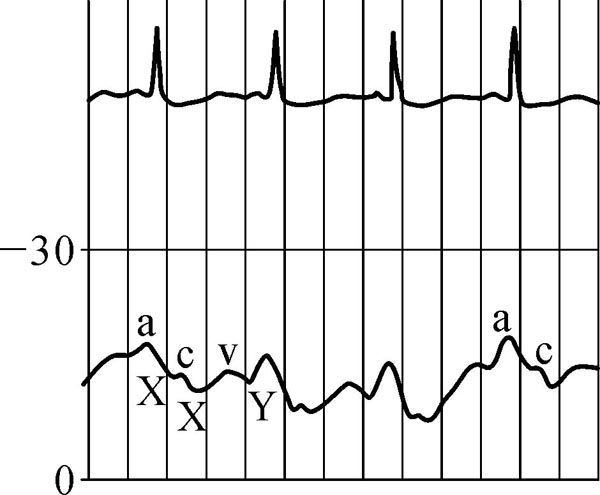
\includegraphics[width=.7\textwidth,height=\textheight,keepaspectratio]{./images/Image00034.jpg}
 \captionsetup{justification=centering}
 \caption{阻塞性脑积水\\{\small  A、B为同一患者,第三脑室、侧脑室扩大(第四脑室正常)}}
 \label{fig2-18}}
  \end{figure} 



先天性患者可重度积水,表现幕上大脑半球区为水样低密度,额、顶、颞叶脑实质几乎消失或残留极少,部分枕叶、基底核和丘脑保存(图\ref{fig2-10})。

\textbf{【鉴别诊断】}
与交通性脑积水鉴别时,如果阻塞在中脑导水管或以上,由于第四脑室不扩大,则两者容易鉴别。如阻塞部位在第四脑室出口时则两者难以鉴别。脑池造影观察第四脑室与蛛网膜下腔的通畅情况有助于鉴别。

\subsection{脑积水与脑萎缩的鉴别诊断}

主要有以下几点:①脑积水的扩大是均匀性和中心性扩张,尤其侧脑室前角呈气球状;而脑萎缩的脑室形态改变不及脑积水明显,特别是室旁脑组织较少的部位变形轻微,如第三脑室前壁、漏斗隐窝和视隐窝。②脑积水时由于颅内压力较高,脑沟变浅或消失,脑池亦不增大;而脑萎缩涉及皮质时脑沟加深、脑池扩大。③阻塞性脑积水和脑萎缩均可致一侧脑室扩大或一侧脑室扩大明显。在阻塞性脑积水时脑室可向扩大或扩大明显的对侧移位;而脑萎缩则向同侧移位。④脑积水侧脑室旁白质内可见间质性水肿所致的低密度;但脑萎缩因室旁白质变性亦可出现低密度灶。⑤脑萎缩是以白质为主的萎缩,表现为侧脑室边缘不规则,有助于与脑积水鉴别。

\section{脑萎缩}

\subsection{概述}

\subsubsection{脑变性疾病和脱髓鞘疾病的概念}

这是两组病变累及部位不同的神经系统疾病。前者累及神经元(灰质);后者累及髓鞘(白质),为髓鞘脱失,而轴索相对完好(见本章第十一节)。但两者均可引起脑萎缩。

变性疾病的特点是某一或二个功能系统的神经细胞发生萎缩和死亡,星形细胞增生。受累部位不同,临床表现也不同。如累及大脑皮质主要表现为痴呆;累及基底节、锥体外系则引起功能障碍;累及小脑引起共济失调。

脑变性疾病按部位分为:①大脑皮质:如Alzheimer病、Pick病。②基底节及脑干:如Jakob-Creutzfeldt综合征、Huntington舞蹈病、Parkinson病、进行性核上麻痹、Sky-Drager综合征。③脊髓及小脑:如橄榄桥脑小脑萎缩、原发性小脑萎缩、共济失调性毛细血管扩张症。④运动神经元:如脑萎缩性侧索硬化、脊髓性肌萎缩。

\subsubsection{脑萎缩的概念}

1.脑萎缩:是指由于各种原因所引起的脑组织减少而继发的脑室和蛛网膜下腔扩大。这种脑组织减少可分别或同时累及脑白质和脑灰质,其病因很多。根据其累及范围可分为局限性和弥漫性两类,但有时两者很难完全分开。

2.局限性脑萎缩:脑实质以局限性容积缩小为主,表现为局限性脑沟增宽和脑室、脑池扩大,有时仅发生于一侧半球。此外,还可见局部脑组织密度下降。

3.弥漫性脑萎缩:脑实质的减少为弥漫性,表现为脑室和蛛网膜下腔扩大广泛(图\ref{fig2-19})。可根据累及灰、白质程度的不同将其分为皮质型和中央型。前者以累及灰质为主,脑沟增宽明显,而脑室扩大次之;后者主要累及白质,以脑室扩大为主,脑沟扩大为次。

\begin{figure}[!htbp]
 \centering
 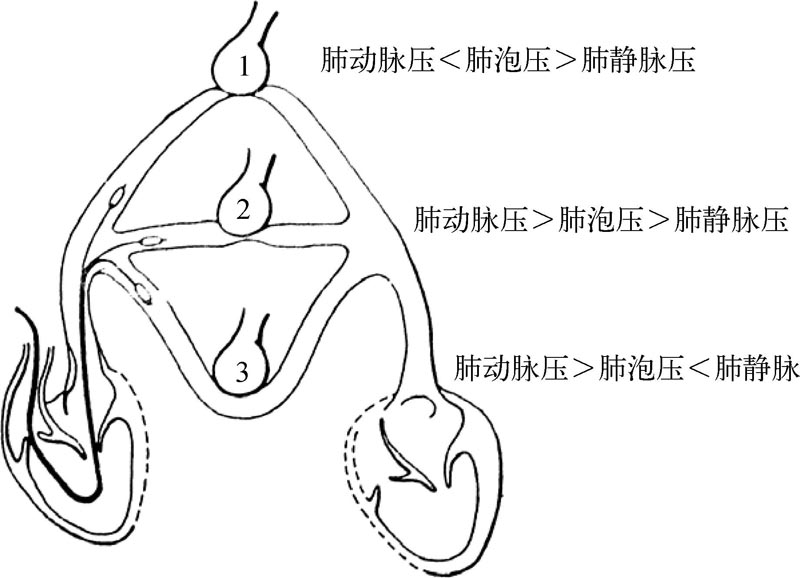
\includegraphics[width=.7\textwidth,height=\textheight,keepaspectratio]{./images/Image00035.jpg}
 \captionsetup{justification=centering}
 \caption{弥漫性脑萎缩\\{\small 脑室和蛛网膜下腔广泛扩大,室旁白质内有低密度灶,侧脑室边缘不规则}}
 \label{fig2-19}
  \end{figure} 



\subsubsection{局限性脑萎缩的病因}

1.外伤性脑萎缩:一般发生在外伤3~6个月后,少数外伤可造成弥漫性脑萎缩。

2.感染后脑萎缩:多继发于脑脓肿,颅内低毒性感染有时可造成弥漫性脑萎缩。

3.脑梗死后脑萎缩:一般发生在发病后3~6个月。

4.Pick病:又称脑叶萎缩症,系常染色体显性遗传性疾病。多见于女性,病程5~6年,呈进行性恶化。临床表现智力低下、痴呆、共济失调等,与Alzheimer病难以区别。但本病以额叶和颞叶萎缩为主,尤其以两额叶为著;而Alzheimer病为弥漫性脑萎缩,且以颞叶较著,额叶多不明显。

5.大脑半球萎缩:由于胎儿期或新生儿期血管阻塞引起的大块脑梗死所致,一般在青少年期才被发现。

\subsubsection{弥漫性脑萎缩的病因}

临床上较局限性脑萎缩更常见,多见于正常老年人,亦可见于许多病理情况。①Alzheimer病;②Huntington病;③Parkinson病;④Wilson病;⑤脑缺氧;⑥Jakob-Creutzfeldt综合征;⑦肿瘤和代谢失调:均与脑组织营养障碍有关(肿瘤患者虽无脑转移瘤,但可有营养障碍),同样情况也可见于AIDS、肝性脑病、血液透析者、慢性酒精中毒和肥胖病人;⑧药物性脑萎缩:如类固醇、氨基甲叶酸、度冷丁、酒精等使用不当。

\subsection{老年脑(生理性脑萎缩)}

关于老年脑的临床意义,目前认识尚不统一。这是因为正常情况下随着年龄的增加,脑组织和其他器官一样,逐渐老化而发生萎缩即所谓生理性萎缩。但随着年龄的增加,易发生的高血压、脑动脉硬化等因素均可损害脑组织而发生萎缩,这种萎缩虽与年龄有关,却为病理性。相对而言生理性萎缩较病理性萎缩轻,但两者无明显界限。

\textbf{【CT表现】}
老年脑主要表现为脑室、脑池轻度扩大和脑沟轻度增宽,多为两侧对称。脑沟增宽以额叶、镰旁顶叶显著,脑室扩大以侧脑室额角、颞角和第三脑室显著。

\subsection{Alzheimer病(爱茨海默病)}

本病以往曾称为早老性痴呆或老年前期痴呆,是一种以弥漫性脑萎缩(但以颞叶为主)为特征的痴呆。本病与老年性痴呆只有年龄上的差异而无本质的区别,故国际上将两病合并称为Alzheimer型痴呆。

\textbf{【病理】}
主要病理表现为脑萎缩,尤其是颞叶海马萎缩为主。镜下脑组织神经细胞减少,尤其有大量老年斑和神经纤维缠结时有定性价值,神经元空泡颗粒变性和淀粉样血管病变,但均为非特异性的,可见于老龄脑。

\textbf{【临床表现】}
其特征为进行性记忆力减退,语言和行为障碍。生前主要依据神经心理测验确立诊断。其病程不可逆转,一般持续3~10年,最后继发感染和全身衰竭而导致死亡。

\textbf{【CT表现】}
①弥漫性脑萎缩表现,与老年性脑萎缩相似,无特征性。②内侧颞叶萎缩是本病最早、最敏感的指征,以海马萎缩最突出,其次为额顶叶。主要表现为颞角扩大,颞叶皮质萎缩和海马回密度减低。有人取负于听眦线20\textsuperscript{o}
平面为扫描基线,层厚5mm,在环池水平测量颞角内侧边与环池外侧边的最小距离即中颞叶最小宽度,其参考值为8.67mm,小于此值即为中颞叶萎缩。③胼胝体萎缩为本病的另一指征,以嘴部和压部最为明显。④在海马萎缩的同时,MR、ECT(PET)等所显示的特异性区域血流量下降也可作为本病的特异性表现。

\textbf{【鉴别诊断】}
主要应于血管性痴呆鉴别。后者在我国老年人中占痴呆疾病的首位(西方占第二位),其颞角扩张不及Alzheimer病明显。严重的皮层下和脑室周围白质病变是多发性梗死型痴呆较典型的表现。

\subsection{慢性进行性舞蹈病}

本病又称遗传性舞蹈病、亨廷顿(Huntington)病,是基底节和大脑皮质变性的一种常染色体显性遗传性疾病。

\textbf{【病理】}
以尾状核及壳核萎缩明显,后期则额、顶叶皮质萎缩。镜下见神经元减少和胶质细胞增生。其生化改变为基底节中多巴胺含量过多,而γ-氨基丁酸及胆碱的含量减少。

\textbf{【临床表现】}
好发于20~50岁,其特征为慢性进行性舞蹈样动作和痴呆,多有遗传和家族史。

\textbf{【CT表现】}
主要为尾状核及壳核的萎缩。两侧尾状核头、体部相对缩小,可伴或不伴侧脑室(尤其额角)扩大和脑沟增宽,两侧壳核对称性低密度。一般只要出现尾状核萎缩即可以做出诊断,小脑和脑干也可萎缩。

\subsection{Parkinson病(帕金森病)}

本病又称震颤麻痹,可分为原发性和继发性两类。前者病因不明;后者可因脑动脉硬化、挫伤、基底节肿瘤、药物和化学物质中毒所致,又被称为Parkinson综合征。

\textbf{【病理】}
肉眼变化的特点是黑质和兰斑脱色。镜下可见该处的神经黑色素细胞丧失。黑质和苍白球神经元明显减少,局部萎缩及黑色素退变。中脑黑质致密带色素细胞大量丢失,桥脑兰斑色素细胞明显减少,脑有对称或非对称萎缩。黑质与兰斑均属儿茶酚胺能核团,分泌多巴胺;尾状核、壳核的神经元属胆碱能细胞,分泌乙酰胆碱。由于黑质神经元大量丧失,使多巴胺含量下降,从而使得对纹状体区乙酰胆碱的抑制作用下降,出现震颤麻痹。

\textbf{【临床表现】}
发生于中年以上,起病很缓慢,逐渐加剧。主要症状包括震颤、肌张力高(强直)、运动障碍、假面具样面容等。

\textbf{【CT表现】}
无特异性,主要为脑室扩大和弥漫性脑萎缩,有时合并基底节钙化,后者亦可见于正常人。CT所示的脑萎缩与临床所见的震颤麻痹的严重程度无明显关系。MR可有黑质(致密带)的萎缩及异常铁质沉积所致的低信号。

\subsection{肝豆状核变性}

本病又称Wilson(威尔逊)病,是一种常染色体隐性遗传的铜代谢障碍性疾病。

\textbf{【病理】}
由于肝脏合成血浆铜蓝蛋白的能力下降,引起肝脏、大脑基底节区和角膜的铜沉积,亦可累及额叶皮质、红核、黑质及齿状核及肾等处。脑受累部位变性、萎缩、胶质增生,甚至缺血坏死、软化。以豆状核软化、角膜色素环(K-F环)及小叶性肝硬化为三大主征。

\textbf{【临床表现】}
好发于10~25岁青少年,约1/3有家族史。基底节损害症状包括进行性加剧的震颤、僵直与多动症,皮质损害为衰退型精神障碍,有肝硬化和角膜色素环表现。

\textbf{【CT表现】}
少数可无异常发现。主要表现为豆状核低密度区,多为双侧,使豆状核界限不清。低密度区还可累及尾状核、齿状核、红核、额叶和丘脑等,部分还可见尾状核、大脑和小脑萎缩。

\textbf{【鉴别诊断】}

1.代谢性疾病:其中以肝豆状核变性最常见,还有亚急性坏死性脑脊髓病(Leigh病)、维生素B\textsubscript{1}
缺乏症,以及线粒体脑病、Kearns-Sayre综合征、海绵状脑白质营养不良、黏多糖病、Hallervorden-Spatz病、岩藻糖苷沉积症、先天性丙酮酸代谢障碍。

2.感染性疾病:EB病毒性脑炎、乙脑和腮腺炎病毒性脑炎等。

3.中毒性疾病:以一氧化碳中毒最常见,还有变质甘蔗中毒、大量硫化氢吸入中毒、甲醇中毒和氰化物中毒等。

此外,纹状体黑质变性(40~50岁发病,病程渐进,以帕金森综合征为首见症状,为锥体外系疾病或列入多系统变性)也可出现双侧壳核对称性低密度及全脑萎缩。国内有学者报道1例静脉窦血栓形成致双侧基底节对称性低密度。我们遇见1例尿毒症患者,表现为以内囊后肢为中心,部分涉及双侧豆状核的低密度。

\subsection{皮质纹状体脊髓变性}

本病又称Jakob-Creutzfeldt综合征、亚急性海绵状脑病、传染性病毒性痴呆。过去一直被纳入变性范围,现多认为是一种病毒感染性疾病。

\textbf{【病理】}
出现以灰质为主的明显脑萎缩。镜下皮质、大脑基底节、脊髓、小脑、丘脑、脑干及脊髓前角神经元变性。神经细胞脱失,脑实质空泡化伴胶质细胞增生,病灶区如海绵状,无炎性变化,白质多正常,晚期可受累。

\textbf{【临床表现】}
好发于40~70岁,主要表现为迅速发展的精神衰退和痴呆,并可出现锥体束、锥体外系及共济失调症状。80%死于发病后1年左右。

\textbf{【CT表现】}
大脑皮质弥漫性萎缩,脑沟、裂增宽增深,亦可见两侧脑室扩大。晚期脑白质受累可见低密度,无占位效应,无强化。本病进展快,短时间随访明显加重。

\subsection{小脑萎缩}

\textbf{【病因】}
本病可由变性性疾病、中毒、慢性酒精中毒、滥用药物等引起。发生于儿童的共济失调性毛细血管扩张症亦表现为以蚓部为主的小脑萎缩。此外橄榄桥脑小脑萎缩(或称橄榄桥脑小脑变性)也是共济失调的一个类型。

\textbf{【病理】}
病变主要在小脑、小脑脊髓束、锥体束、橄榄核,甚至累及大脑皮质,小脑萎缩皮质重于髓质。橄榄桥脑小脑萎缩除小脑萎缩外,还有桥脑、橄榄的明显萎缩,大脑皮质也可受累。

\textbf{【临床表现】}
成年发病,病程缓慢,可为10~40年。表现为小脑性共济失调,锥体束征、锥体外系征、视神经萎缩。

\textbf{【CT表现】}
应包括以下两个或两个以上征象(图\ref{fig2-20}):①小脑沟增宽>1mm(也有人认为\textgreater{}2mm);②小脑沟在半球超过2条,蚓部超过4条;③桥小脑角池扩大>1.5mm(应测量小脑上边缘与岩骨边缘间的距离);④第四脑室扩大;⑤小脑上池扩大。

\subsection{精神分裂症}

本病多有脑结构的异常。

\begin{figure}[!htbp]
 \centering
 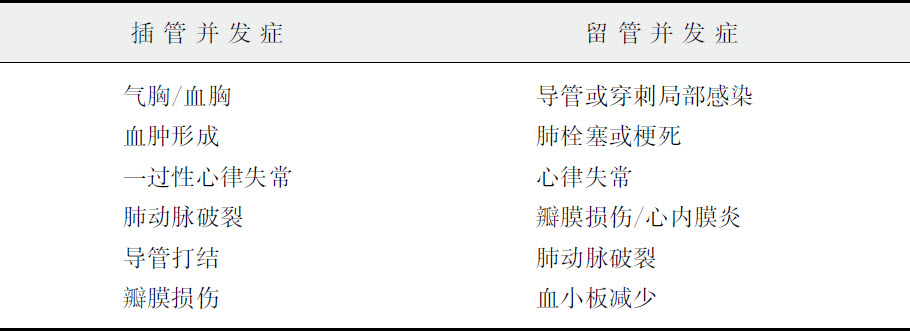
\includegraphics[width=.7\textwidth,height=\textheight,keepaspectratio]{./images/Image00036.jpg}
 \captionsetup{justification=centering}
 \caption{小脑萎缩\\{\small 小脑沟显著增宽、增多,以蚓部为著}}
 \label{fig2-20}
  \end{figure} 



\textbf{【CT表现】}
第三、第四脑室扩大,两侧裂池增宽、脑沟扩大,有时出现侧脑室扩大和小脑萎缩。两侧室旁核和小脑的密度可增加,其意义尚不肯定。

\subsection{颞叶癫痫}

颞叶癫痫的常见原因为海马硬化(又称安蒙氏角硬化和颞叶中内侧硬化)。

\textbf{【病理】} 特征为神经元丢失和胶质细胞增生,导致海马的萎缩。

\textbf{【CT表现】}
其CT诊断价值较小,仅约23.8%有异常。表现为:①颞叶内侧低密度灶;②颞角扩大;③侧裂池增宽。

\textbf{【MR表现】} 海马的萎缩(为神经元丢失的反应)、T\textsubscript{2}
WI海马高信号(为胶质细胞增生的反应)、颞叶前部萎缩以及颞角扩大。

\section{脑缺血、出血和脑血管病变}

\subsection{动脉缺血性脑梗死}

脑组织因血管阻塞引起缺血性坏死或软化称为脑梗死。广义的脑梗死除动脉缺血性脑梗死外,还包括静脉血流受阻所致的脑梗死即静脉性脑梗死。但大多习惯于狭义的将动脉缺血性脑梗死称为脑梗死。

\textbf{【病因】}
引起梗死的原因很多,可分为两大类。①脑血管阻塞:又分为血栓形成和栓塞。前者最常见的是在动脉粥样硬化的基础上形成血栓;后者是指外来栓子堵塞血管所致。②脑部血液循环障碍:是指在脑血管原有病变的基础上(亦可无原发血管病变),由各种原因造成的脑组织供血不全而引起的梗死,故又称非梗阻性脑梗死。

\textbf{【病理】}
过去将脑梗死分为3个时期,即梗死期、吞噬期、机化期。目前通常将脑梗死分为:①超急性期:6小时以内;②急性期:6小时后~2天;③亚急性期:2天后~2周内;④慢性早期:2周~1个月;⑤慢性晚期:1月后(见表\ref{tab2-2})。

\begin{table}[htbp]
\centering
\caption{脑梗死的病理过程及CT表现}
\label{tab2-2}
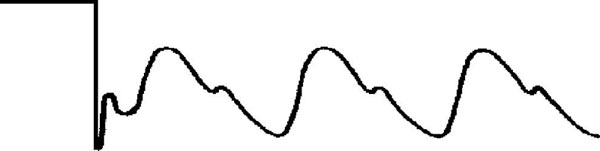
\includegraphics[width=\textwidth,height=\textheight,keepaspectratio]{./images/Image00037.jpg}
\end{table}

脑供血完全终止后数秒钟神经元电生理活动停止,持续5~10分钟以上就有不可恢复的细胞损伤。但是临床上供血血管闭塞可能不完全和(或)存在侧支循环,仅使局部血流降低到一定程度。故部分脑组织虽有缺血损伤,但仍可恢复正常,这部分脑组织区域称为缺血半暗带。它位于缺血坏死核心与正常脑组织之间。但如超急性期治疗不及时或治疗无效可发展成为完全脑梗死。

少数缺血性脑梗死在发病24~48小时后可因再灌注而发生梗死区内出血,称为出血性脑梗死。

\textbf{【临床表现】}
临床表现复杂,取决于梗死灶大小、部位及脑组织的病理生理反应。主要表现为头昏、头痛,部分有呕吐及精神症状,可有不同程度的昏迷。绝大多数出现不同程度的脑部损害症状,如偏瘫、偏身感觉障碍、偏盲,亦可失语、抽搐,较重者可有脑疝症状。从解剖学可知,皮质脊髓束有10%的纤维不交叉下降,加入同侧皮质脊髓侧束。皮质脊髓前束也有少量纤维不交叉,止于同侧颈、胸髓。这些不交叉的运动传导纤维支配了同侧肢体运动,当这些纤维受损时,导致同侧肢体出现不同程度的运动功能障碍如麻木、无力,甚至偏瘫。

\textbf{【CT表现】}

1.超急性期脑梗死的CT表现:①大脑中动脉高密度征:为高密度血栓或栓子所致,出现率约占35%~45%(敏感度78%,特异度93%),但需除外血管硬化因素。最近研究表明,此征可见于近60%的正常人(尤其用7mm以下层厚扫描),故此征的诊断价值值得怀疑。②脑实质低密度征:可能为细胞内水肿所致,可见于脑的凸面、基底节区、岛叶,有时可伴侧裂池受压。③局部脑组织肿胀征:可能为血管源性水肿所致,局部脑沟变窄以至消失,脑回增厚、变平(图\ref{fig2-21}A)。脑CT灌注成像有利于超急性期脑梗死的诊断。

此外,脑血管CTA可显示闭塞部位、程度和侧支循环情况。

许多学者研究证实,CT灌注成像可以预测半暗带,即脑血流量(rCBF)中度减低时,局部脑血容量(rCBV)无明显变化或仅有轻度下降或轻度升高,此时缺血区微血管管腔受压、变形、闭塞的程度较轻。当rCBF和rCBV均明显减低时,提示脑局部微血管管腔闭塞程度明显、微循环发生障碍、脑组织发生梗死。国内有学者将面积\textsubscript{CBV}
定义为预测的梗死面积,则面积\textsubscript{CBF} -
面积\textsubscript{CBV} 为预测的半暗带面积。

2.典型CT表现:①脑组织低密度灶,呈楔形或三角形,病灶部位、范围与闭塞动脉供血区相吻合。大脑中动脉主干闭塞,病灶呈三角形低密度区,尖端指向第三脑室;大脑中动脉闭塞在豆纹动脉的远端,病灶多为矩形低密度区,出现“基底核回避现象”。大脑前动脉闭塞表现为位于大脑镰旁的长条状低密度区。大脑后动脉闭塞在顶叶后部及枕叶可见半圆形的低密度区,位于大脑镰旁的后部。局灶性脑皮质梗死,表现为脑回丢失。室管膜下脑梗死,脑室边缘呈波浪状。一般在发病24小时后出现以上表现(图\ref{fig2-21}B、C)。②2~3周时由于“模糊效应”,病灶可偏小或消失。③脑梗死后2~15天为水肿高峰期,可有占位效应,占位效应一般见于病变范围大的病例。如占位效应超过1个月,应注意有无肿瘤可能。④增强扫描病灶周围和病灶内出现脑回状、线状、团块状强化。⑤1个月后病灶开始软化呈水样密度,病变范围大的病例可继发局限性脑萎缩。

此外,出血性脑梗死在梗死区内可见高密度出血灶(图\ref{fig2-21}D)。



\begin{figure}[!htbp]
 \centering
 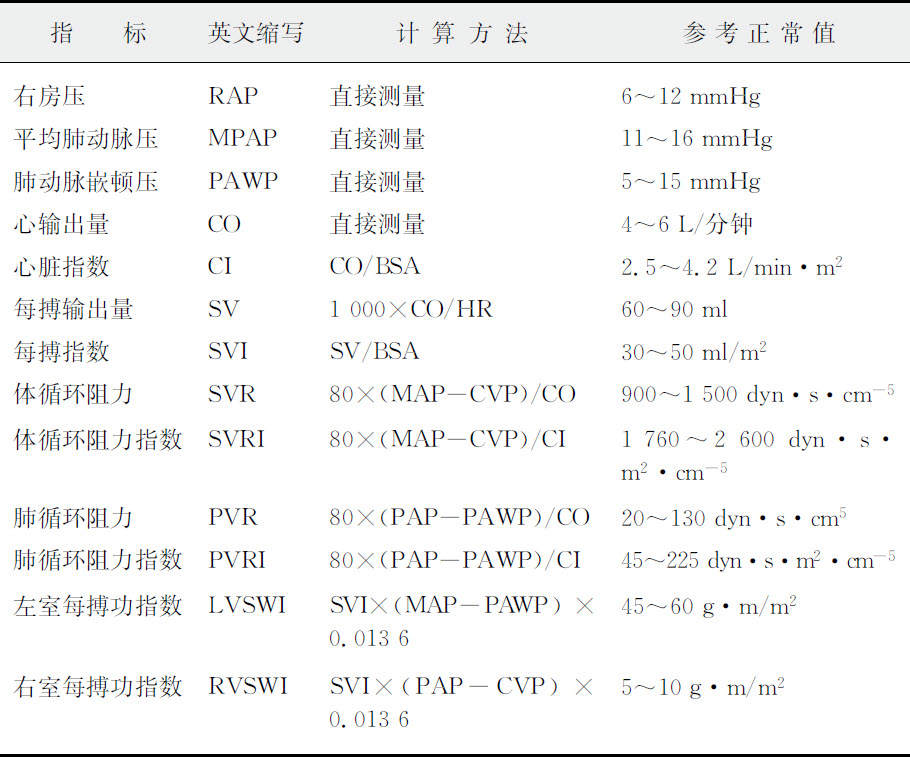
\includegraphics[width=\textwidth,height=\textheight,keepaspectratio]{./images/Image00038.jpg}
 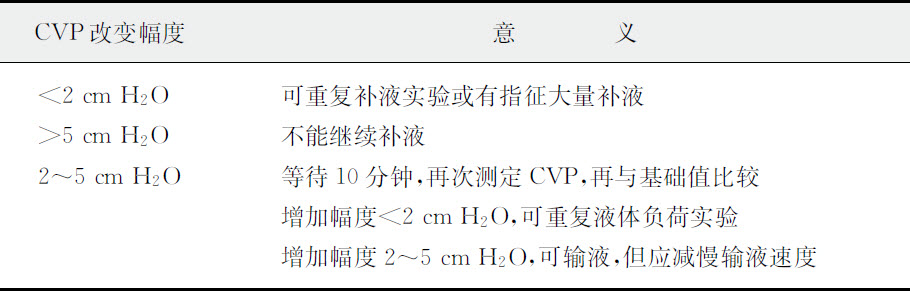
\includegraphics[width=\textwidth,height=\textheight,keepaspectratio]{./images/Image00039.jpg}
 \captionsetup{justification=centering}
 \caption{脑梗死\\{\small A、B为同一患者。A.超急性期,发病后4小时,右侧额顶叶脑沟消失,皮髓质交界不清晰;B.发病后42小时,右侧颞额顶叶大片状低密度灶,界限清晰,显著占位效应;C.亚急性期脑梗死,左侧顶额叶区有大片楔形低密度区,占位效应较显著;D.出血性脑梗死,右侧颞额叶区有大片楔形低密度区,占位效应显著,其内见大片状高密度出血灶,左侧基底节区可见水样密度的软化灶}}
 \label{fig2-21}
  \end{figure} 

3.增强扫描CT表现:梗死灶强化的形态多种多样,可表现为脑回状、线状、片状、环状,可出现在病灶的边缘和中心。而延迟30分钟~3小时扫描可显示皮质下白质强化,可能与梗塞区皮质内大量毛细血管破坏,造影剂漏出有关。其强化机制与缺血区血脑屏障受损,新生的毛细血管大量增生,以及局部血流量增加有关。但在1周内,虽有血脑屏障的破坏,却因局部缺血坏死严重,造影剂浓度亦相应很低,故一般不出现强化。梗死7~10天后因局部大量毛细血管增生,血流量增大而出现明显强化。2~3周发生率最高,强化最明显,可持续1个月或更久。

\textbf{【鉴别诊断】}
应注意与胶质瘤、转移瘤、脱髓鞘病变和脑脓肿等鉴别。①脑梗死常累及皮质和白质两部分;而上述病变一般只造成白质低密度。②脑梗死的分布为某一动脉区或分水岭区,有一定特征;而脑肿瘤和炎症水肿沿白质通道扩散,无明显分布规律,常呈指状低密度区;脱髓鞘低密度灶常对称性分布在侧脑室周围。③增强扫描胶质瘤常出现不均匀强化,有时可见壁结节;转移瘤常可见多灶强化。

\subsection{脑梗死前期}

从脑血流量(CBF)变化过程看,脑血流量的下降到急性脑梗死的发生经历了3个时期。首先,由于脑灌注压下降引起的脑局部的血流动力学异常改变;其次,脑循环储备力失代偿性低灌注所造成的神经元功能改变;最后,由于CBF下降超过了脑代谢储备力才发生不可逆转的神经元形态学改变即脑梗死。国内高培毅将前两者称为脑梗死前期,它不同于超急性期脑梗死。

他们根据脑局部微循环的变化程度以及CT灌注成像表现包括局部脑血流量(rCBF)、局部脑血容量(rCBV)、平均通过时间(MTT)和峰值时间(TTP)参数图,将脑梗死前期分为2期4个亚型:

Ⅰ期:脑血流动力学发生异常变化,脑血流灌注压在一定范围内波动时,机体可以通过小动脉和毛细血管平滑肌的代偿性扩张或收缩来维持脑血流相对动态稳定。

Ⅰ\textsubscript{1}
:脑血流速度发生变化,脑局部微血管尚无代偿性扩张。灌注成像见TTP延长,MTT、rCBF、rCBV正常。

Ⅰ\textsubscript{2} :脑局部微血管代偿性扩张。灌注成像见TTP
和MTT延长,rCBF正常或轻度下降,rCBV正常或轻度升高。

Ⅱ期:脑循环储备力失代偿,CBF达电衰竭阈值以下,神经元的功能出现异常,机体通过脑代谢储备力来维持神经元代谢的稳定。

Ⅱ\textsubscript{1}
:CBF下降,由于造成局部星形细胞足板肿胀,并开始压迫局部微血管。灌注成像见TTP
和MTT延长,以及rCBF下降,rCBV基本正常或轻度下降。

Ⅱ\textsubscript{2}
:星形细胞足板明显肿胀,并造成局部微血管受压变窄或闭塞,局部微循环障碍。灌注成像见TTP
和MTT延长,rCBF和rCBV下降。

\subsection{分水岭性脑梗死}

即指两条主要脑动脉供血交界区发生的脑梗死。

\textbf{【病因】}
①血液动力学障碍:低血压(如心肌梗死、心律失常、体位性低血压)等所致的血液动力学障碍;②血管调节功能失常:如糖尿病并发植物神经功能紊乱、长期低血压;③高血压病过分降压治疗;④心脏附壁血栓脱落沿血管进入脑皮质支和深穿支。

\textbf{【CT表现】}
①皮质下型:多为白质内低密度,常呈条形或类圆形。灰质由于血流再灌注而呈等密度,但灰质可出现明显强化。②皮质前型:额顶叶交界区三角形、条形低密度灶。③皮质后型:颞顶枕叶交界区三角形、条形低密度灶。

\subsection{血液动力性脑梗死}

当脑外动脉狭窄、部分阻塞和痉挛时,一般情况下尚能维持脑组织的血供。但当某些原因引起较长时间的血压下降时,可造成狭窄动脉供血脑组织的严重缺血而发生脑梗死,这种梗死称为血液动力性脑梗死。

\textbf{【病因病理】}
心律失常、心功能不全、休克、高血压过分降压等是其常见原因。严重的低血压和心搏量降低如心肌梗死、外科手术等,即使患者无颅内外血管病变,也可引起大脑半球的广泛梗死。血液动力性脑梗死多为分水岭性脑梗死。

\textbf{【CT表现】}
与分水岭性梗死的表现相似,可见条形或类圆形低密度,也可广泛梗死,这种梗死以分水岭区最著。可累及基底节区和小脑,皮质可强化。

\subsection{腔隙性脑梗死}

即指脑深部2~15mm大小的脑梗死。

\textbf{【病因】}
多为高血压、糖尿病、动脉硬化、高脂血症所致。好发于基底节、丘脑、内囊区、深部室旁白质及脑干。这些部位的血管多远离大脑主干,细长且走行弯曲,对血液动力学变化敏感,易受缺血影响。

\textbf{【临床表现】}
纯运动性偏瘫、纯感觉障碍、下肢运动受限、构音困难、视力障碍、失语、短小步态及共济失调等。

\textbf{【CT表现】}
梗死灶在2~15mm之间,呈圆形或卵圆形低密度,边缘不清,无水肿和占位效应。3~4周后可形成边缘清楚的囊性软化灶(图\ref{fig2-22})。

\begin{figure}[!htbp]
 \centering
 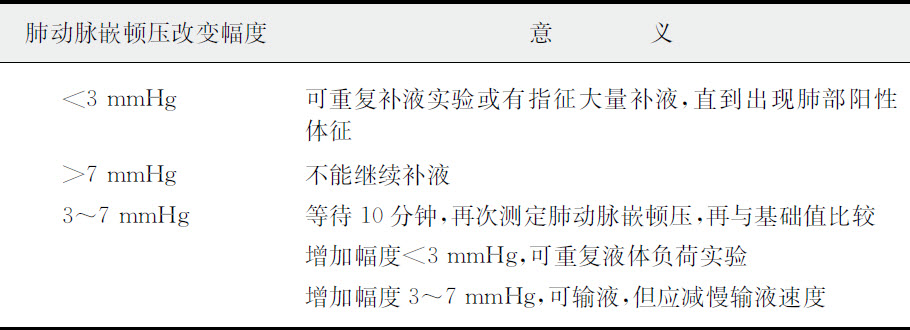
\includegraphics[width=.7\textwidth,height=\textheight,keepaspectratio]{./images/Image00040.jpg}
 \captionsetup{justification=centering}
 \caption{腔隙性脑梗死\\{\small A.病灶位于左侧基底节区和左侧额叶白质区;B.病灶位于脑干}}
 \label{fig2-22}
  \end{figure} 

\textbf{【鉴别诊断】}
脑腔隙在病理上为一脑实质内含水分的<15mm的潜在腔,包括穿支动脉等病变所致的腔隙性脑梗死和非血管病变引起的腔隙病变。发病机制包括血管因素所致的缺血即腔隙性梗死,以及血管因素(如出血、动脉炎等)和血管外因素(如炎症、变性、中毒、机械损伤等)所形成的腔隙性病变,应注意分析。此外,还应注意与前联合及基底节区的扩大的血管周围间隙(多在0.2~1.2cm大小)相鉴别,MR检查有独到鉴别价值。

\subsection{皮质下动脉硬化性脑病}

本病又称Binswanger病,是一组以脑深部小动脉硬化、痴呆、皮质下白质变性、皮质下腔隙或软化为特征的综合征。但有人认为“皮质下动脉硬化性脑病”一词未能正确反映所看到的组织学改变,且过高的估计了临床意义。因此,有关文献应用的非特异性名词较合适,如深部脑白质缺血或老年性白质高信号(MR)。我们认为称为“动脉硬化性脑白质病”或“深部脑白质慢性缺血”更趋合理,同时我们认为有关文献所述及的“脑白质疏松症”亦属本病的范畴。

\textbf{【病因病理】}
主要病因为慢性高血压,其病理特征为弥漫性不完全的皮质下梗死,在侧脑室旁和半卵圆中心的白质内髓鞘肿胀或脱失,皮质下弓状纤维与胼胝体不受累。常有皮质萎缩及皮质下、基底节区腔隙性脑梗死,在髓动脉内有狭窄性动脉粥样硬化。

\textbf{【临床表现】}
见于60岁以上老人,多隐形起病,呈进行性记忆力障碍、严重精神衰退、言语不清,反复发生的神经系统局部体征如偏瘫、失语、偏盲等。病情可缓解和反复加重,常伴有高血压。

\textbf{【CT表现】}
脑白质内斑片状或云絮状稍低密度灶,界限不清,其密度降低不如脑梗死明显。以侧脑室周围分布最明显,其次为半卵圆中心,多为两侧对称性(图\ref{fig2-23})。基底节---内囊区、丘脑、半卵圆中心常伴多发的腔隙性梗死灶,可有脑室系统扩大,脑沟、脑池增宽的弥漫性脑萎缩改变。

\begin{figure}[!htbp]
 \centering
 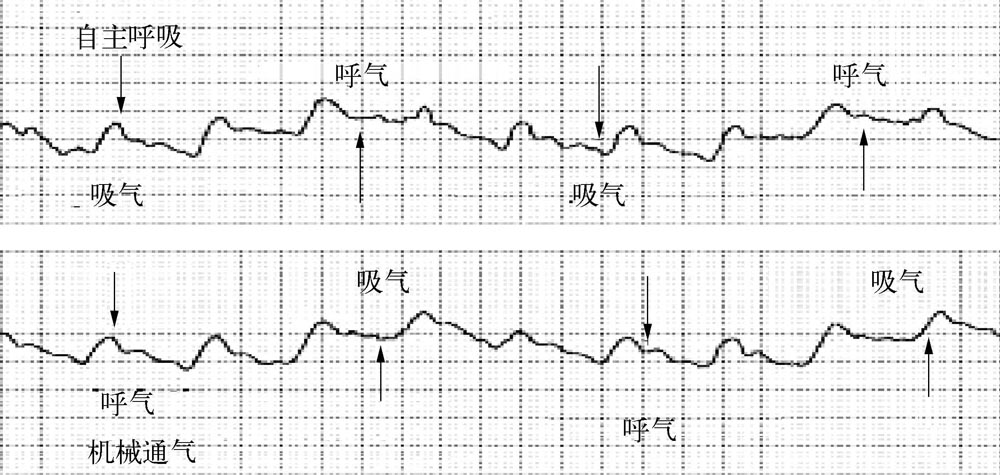
\includegraphics[width=.7\textwidth,height=\textheight,keepaspectratio]{./images/Image00041.jpg}
 \captionsetup{justification=centering}
 \caption{动脉硬化性脑白质病\\{\small 侧脑室周围白质和半卵圆中心区对称性片絮状低密度灶}}
 \label{fig2-23}
  \end{figure} 

\subsection{脑缺氧}

\textbf{【病因病理】}
脑缺氧包括乏氧性缺氧、血液性缺氧、循环性缺氧和中毒性缺氧。常见病因有:高空高原缺氧,呼吸功能不全和某些先心病循环短路、CO中毒以及各种严重贫血、各种休克和心衰,氰化物、硫化氢、磷中毒。脑组织局部循环性缺氧包括颅脑外伤、脑血管意外、脑血流障碍、颅内感染、脑肿瘤急性恶化等。主要病理改变为早期脑组织坏死、水肿,进行性脱髓鞘,晚期脑萎缩。

\textbf{【CT表现】}
①弥漫性脑水肿:以大脑为主,可出现大脑密度普遍减低,而丘脑、脑干和小脑密度相对较高的所谓CT反转征。②局部脑水肿:以脑动脉边缘带(分水岭区)、脑室周围白质最常见,基底节次之,也可见于丘脑和小脑。③缺氧性脑出血:脑实质、脑室周围-脑室、蛛网膜下腔、硬膜下或硬膜外。④脑萎缩:晚期可出现,也可见囊状软化灶。

\subsection{脑静脉窦血栓形成}

颅内静脉血流受阻即脑静脉和静脉窦血栓形成所导致的脑梗死称为静脉性脑梗死,占中风病人的1%~2%。

\textbf{【病因】}
近1/3病因不明。可分为:①全身因素:脱水、糖尿病、高凝血状态、血小板增多症、口服避孕药、妊娠、产后、近期手术、长期应用激素、肾病综合征、心脏病、结缔组织病、新生儿窒息等;②局部因素:局部感染、中耳乳突炎、鼻窦炎、脑膜炎、颅面中耳手术、颅脑外伤、动静脉畸形、动静脉瘘、腰穿等。

\textbf{【临床表现】}
多见于20~35岁女性,其表现各异。头痛最常见,15%急性起病,类似蛛网膜下腔出血,常伴头晕、恶心及视乳头水肿等颅内高压症状。1/3~1/2病人有局灶性神经症状,如颅神经麻痹和意识障碍,半数出现癫痫,还可有偏瘫。小脑静脉血栓可有共济失调等症状。

\textbf{【CT表现】}
最常见于上矢状窦、横窦和乙状窦,其次为海绵窦和直窦。特征性改变为致密静脉征(或索条征)和空三角征,但缺乏特异性。①早期(1~2天):平扫静脉窦内血栓密度与硬脑膜相似,可高达150Hu。增强扫描呈“空三角征”,即三角形的硬膜窦断面,中心不强化而周围强化。②第3~第10天:平扫窦内血块渐吸收,CT值约80Hu左右。③11天后:血凝块基本吸收,窦内CT值约50Hu。④静脉栓塞常伴有弥漫性非对称性脑肿胀、梗死性脑水肿、出血性梗死或单纯出血(脑实质和硬膜下)。静脉性出血其血肿周围界限不清,多靠近脑表面,而且周围环以大片低密度灶有别于动脉性出血。

\textbf{【鉴别诊断】}
高位分叉的上矢状窦、硬膜下脓肿和血肿、蛛网膜下腔出血及窦内窗孔和分隔均可类似空三角征;儿童的流动性静脉血常呈轻度高密度类似血栓,应注意鉴别。

\subsection{高血压脑病}

本病是指在血压迅速剧烈升高时,引起的急性全面性脑功能障碍,属可逆性后部白质脑病综合征(还见于妊娠高血压、慢性肾衰、使用免疫抑制剂和激素等)的范畴。

\textbf{【病因病理】}
可发生于各种原因(原发或继发)引起的动脉性高血压。病理上大多有不同程度的脑水肿,脑表面动脉、静脉和毛细血管扩张,脑切面可见斑点状、裂隙状出血和小动脉壁的坏死。

\textbf{【临床表现】}
该病一般起病急骤,病程短暂,所有症状历时数分钟或1~2小时,最多数天。主要表现为严重头痛、惊厥、偏瘫、失语、黑蒙、神志不清甚至昏迷。

\textbf{【CT表现】}
主要为广泛性脑水肿,呈对称性、弥漫性、边界不清的低密度区,以大脑半球后部最为显著,也可累及小脑。脑室系统变小,脑沟、脑池变浅。血压改善后一段时间随访,完全恢复正常。

\subsection{脑出血}

脑出血是指脑实质内的出血,又称为脑溢血或出血性脑卒中。

\textbf{【病因病理】}
其原因很多,临床上概括为损伤性和非损伤性两大类。后者又称为原发性或自发性脑出血,是指脑内血管病变、坏死、破裂而引起的出血。自发性脑出血绝大多数由高血压和动脉硬化(引起脑小动脉的微型动脉瘤或玻璃样变)所致,其次为脑血管畸形和动脉瘤所致。其他原因还有颅内肿瘤出血、出血性梗死、脑血管淀粉样变、全身出血性疾病、维生素缺乏、新生儿颅内出血、重症肝炎(可合并脑出血、梗死)等。

出血好发于壳核和内囊区(约占50%)、中心部脑白质、丘脑和下丘脑、小脑半球、桥脑,以及脑室内。病理可分为3期:①急性期:血肿内含新鲜血液或血块,周围脑组织有不同程度的水肿,还可有点状出血;②吸收期:血肿内红细胞破坏、血块液化,周围出现吞噬细胞,并逐渐形成含有丰富血管的肉芽组织;③囊变期:坏死组织被清除,缺损部分由胶质细胞及胶原纤维形成瘢痕,血肿小可由此类组织充填,血肿大时则遗留囊腔。

\textbf{【临床表现】}
本病常突然发生剧烈头痛、意识障碍、恶心、呕吐、偏瘫、失语、脑膜刺激征等,按病情发展可分为急性期、亚急性期和慢性期。

临床预后与出血的部位及出血量的多少有关。出血位于皮质下白质区,血肿及水肿引起占位效应,导致出血区功能丧失,但预后相对较好,出血量>30ml为手术指征。小脑或脑干出血压迫四脑室,继发急性颅内压升高,常伴延髓生命中枢损害,直接危及生命,血肿直径>3cm应立即手术。

\textbf{【CT表现】}
血液形成影像的主要成份为含铁的血红蛋白,血液的密度高于脑组织,故CT表现呈高密度。由于脑血管较细,受部分容积效应影响,故血管内血液多不能显示。严重贫血的患者急性期脑出血亦可呈等密度甚至低密度。

\subsubsection{出血量的估计}

一般采用以下公式计算:V(ml)=1/6
π(A×B×C),A为血肿前后径,B为左右径,C为上下径。A、B、C的单位均为厘米。

\subsubsection{CT分期}

通常将脑内血肿分为急性期(1周内)、吸收期(2周~2个月)和囊变期(2个月后)。也有学者根据密度分为:高密度期、等密度期、低密度期、慢性期(图\ref{fig2-24})。

\begin{figure}[!htbp]
 \centering
 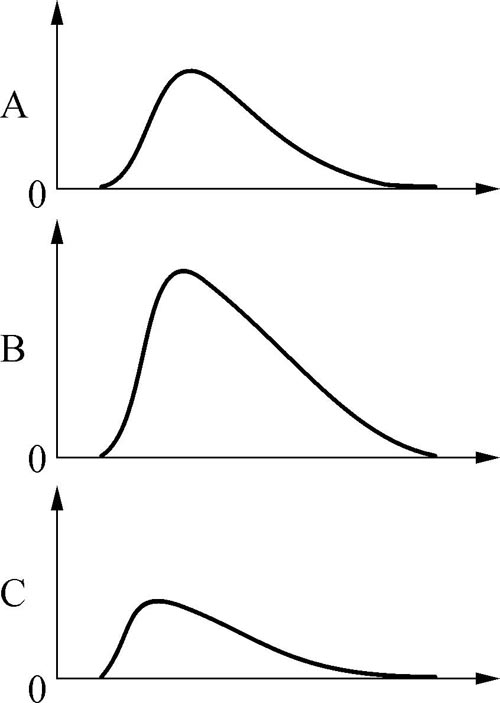
\includegraphics[width=.7\textwidth,height=\textheight,keepaspectratio]{./images/Image00042.jpg}
 \captionsetup{justification=centering}
 \caption{脑出血\\{\small A.右侧丘脑-外囊区血肿破入左右侧脑室内,右外侧裂内亦有血液充填;B.脑出血吸收期,血肿边缘开始吸收呈环状低密度,低密度外可见肉芽组织形成的等密度环}}
 \label{fig2-24}
  \end{figure} 

1.高密度期(1~14天):血液逸出血管后,红细胞分解释放含铁的血红蛋白,表现为高密度区,CT值约50~80Hu。出血3~4天因血液凝固成血块,血浆被吸收,红细胞压积增加,血肿密度达到高峰,甚者达90Hu,周围有水肿。严重贫血者可为等密度,甚至低密度,但血肿有占位征象。

2.等密度期(14~64天):血红蛋白分解,含铁血黄素开始被吸收,血肿呈等密度。但仍有占位效应,水肿仍存在,增强扫描呈环状强化。

3.低密度期(30~84天):血肿周围的新生血管及神经胶质增生形成血肿壁,血肿内含铁血黄素及血红蛋白被吸收,CT呈低密度灶。水肿消失,无占位效应,增强扫描仍呈环状强化。

4.慢性期(3个月后):少量脑出血被胶质和胶原纤维替代而愈合,CT呈略低密度灶。大量脑出血形成囊腔,CT近水样密度,并可出现牵拉现象,增强扫描无或轻微强化。

\subsubsection{脑室内出血}

单纯脑室出血与脑实质内出血破入脑室系统表现一样。少量出血时多沉积在侧脑室后角、第三脑室后部或第四脑室顶部,大量出血常呈脑室“铸型”样表现(图\ref{fig2-25})。早期可有分层现象,以后呈等或低密度,脑室内出血可形成脑积水。

\begin{figure}[!htbp]
 \centering
 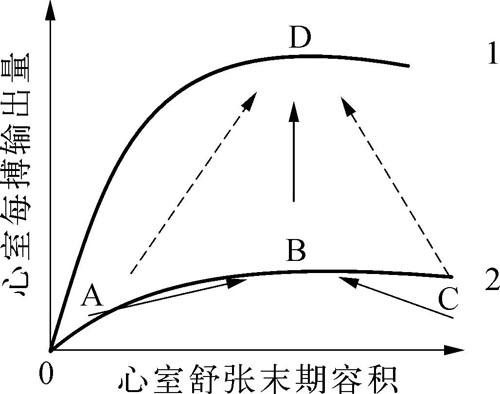
\includegraphics[width=.7\textwidth,height=\textheight,keepaspectratio]{./images/Image00043.jpg}
 \captionsetup{justification=centering}
 \caption{脑室内出血\\{\small 左右侧脑室内有大量血液充填,右侧呈“铸型”样表现}}
 \label{fig2-25}
  \end{figure} 

此外,在诊断时应注意:①急性脑出血大的血肿可形成脑疝。②脑出血可直接破入脑室系统和蛛网膜下腔,亦可由脑室系统进入蛛网膜下腔。③出血周围水肿,在第1天内可出现或表现轻微;3~7天达高峰;出血16天左右占位效应开始减退。④发现灶周水肿与血肿期龄不符时,应考虑肿瘤出血可能。⑤如局部伴有钙化或血肿密度不均等表现,除考虑到肿瘤出血外,也应考虑到脑血管畸形的可能。

\subsection{慢性扩展性脑内血肿}

本病是自发性脑内血肿的一种特殊类型,临床及影像学表现无特异性,易与肿瘤卒中、囊肿合并出血感染等混淆。

\textbf{【病因病理】}
其病因认为与隐匿性血管畸形、血管硬化、外伤、放射损伤、凝血功能障碍有关,一般没有高血压和脑外伤病史。隐匿性血管畸形或微小动脉瘤破裂出血,血肿及其代谢产物不断刺激周围组织产生炎性反应,毛细血管、纤维组织增生,并由增生的毛细血管、纤维组织形成包膜。而其丰富的毛细血管壁脆弱,反复出血、渗出,包膜内液化,使血肿体积逐渐增大。

\textbf{【CT表现】}
多为边缘清楚、密度均匀或不均匀的高、低混杂囊性病灶,且其内可见液-液平面。增强扫描病灶多无强化;部分血肿周围环状强化,为病灶周围脑组织或肉芽组织强化所致。

\subsection{蛛网膜下腔出血}

本病是指颅内血管破裂后血液注入蛛网膜下腔。

\textbf{【病因】}
临床可分为两大类,即外伤性与自发性。自发性原因很多,但以颅内动脉瘤(约占51%)、动静脉畸形(6%)和高血压动脉硬化所致(15%)最多见。此外,20%病因不明。

\textbf{【临床表现】}
自发性常有明显的诱因,如体力劳动过度、咳嗽、用力排便、情绪激动等。绝大多数起病急,剧烈头痛、呕吐、意识障碍、抽搐、脑膜刺激征等,同时可有偏瘫,腰穿有确诊价值。

\textbf{【CT表现】}
一般在出血3天内检出率最高,可达80%~100%,一周后很难检出。特征性表现为基底池、侧裂池和脑沟内等广泛的高密度影(图\ref{fig2-26})。如出血量少或严重贫血均不易发现。大脑前动脉破裂血液多积聚于视交叉池、纵裂前部;大脑中动脉破裂血液多积聚于一侧的外侧裂附近,也可向内流;颈内动脉破裂血液也以大脑外侧裂为多;椎基动脉破裂血液主要积聚于脚间池和环池。但出血量大者可难以估计出血部位。

\begin{figure}[!htbp]
 \centering
 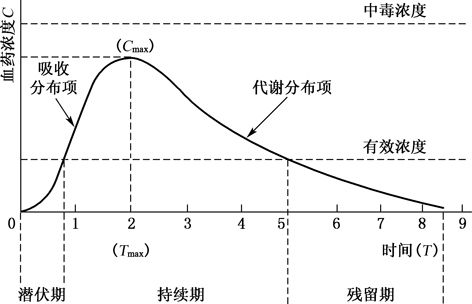
\includegraphics[width=.7\textwidth,height=\textheight,keepaspectratio]{./images/Image00044.jpg}
 \captionsetup{justification=centering}
 \caption{蛛网膜下腔出血\\{\small A、B为同一患者,鞍上池、左右外侧裂池、纵裂池前部、环池、四叠体池、大脑大静脉池内均有大量高密度血液充填}}
 \label{fig2-26}
  \end{figure} 

\textbf{【并发症】}
①脑积水:脑积水早期为梗阻性,发生率约为20%。可演变成交通性。②脑动脉痉挛:造成脑缺血和脑梗死,发生率约25%~42%。③伴发脑内血肿和(或)硬膜下血肿、脑室内出血:常与动脉瘤、动静脉畸形或脑肿瘤出血有关。

\subsection{颅内动脉瘤}

动脉壁呈局限性病理性扩张,与动脉腔有一颈部相连。

\textbf{【病因病理】}
其病因有先天性因素、动脉粥样硬化、感染因素和外伤4个方面。根据影像学可分为5种病理类型:①粟粒状动脉瘤;②囊状动脉瘤;③假性动脉瘤;④梭形动脉瘤;⑤壁间动脉瘤。

\textbf{【临床表现】}
好发于20~70岁。在破裂前90%无特殊临床症状,少数可影响到邻近神经或脑结构而产生症状。破裂后引起蛛网膜下腔出血和颅内血肿而出现相应的症状体征。

\textbf{【CT表现】}
颅内动脉瘤好发于脑动脉,约90%~95%分布于颈内动脉系统,5%~10%分布于椎动脉系统。颈内动脉瘤约占20%~40%,大脑中动脉瘤约占21%~31%,前交通及大脑前动脉瘤约占30%~37%,多发性约占4%~5%。

1.颅底较小动脉瘤:平扫难以显示,增强扫描呈高密度。

2.较大动脉瘤:平扫呈圆形等或高密度,边缘光整,有时瘤壁可见钙化。增强扫描呈均匀强化,而血栓无强化。

3.巨大动脉瘤:即直径>2.5cm的动脉瘤,其CT表现可分3型。①无血栓形成型:平扫呈圆形或椭圆形等或略高密度,瘤壁钙化较其他类型少见。增强扫描均匀强化。②部分血栓形成型:最常见,呈圆形或卵圆形略高密度,壁多有弧形钙化。增强扫描流动的血液强化明显,血栓不强化,从而形成高密度影内的低密度点称为“靶征”。周围很少有水肿。③完全栓塞型:平扫为圆形或卵圆形混杂略高密度,瘤壁常有钙化,周围无水肿。增强扫描呈环状强化。

此外,CTA显示动脉瘤的敏感性可达95%,特异性近83%。

\textbf{【并发症】}
①颅内出血:蛛网膜下腔出血、脑内血肿和脑室内积血,甚至可穿破蛛网膜造成硬膜下血肿。②脑血管痉挛:蛛网膜下腔出血所致,并导致相应区域的水肿、梗死。③脑积水:蛛网膜下腔出血所致。

\textbf{【鉴别诊断】}
动脉瘤周围多无水肿,瘤壁可有环形强化,动态CT扫描时间-密度曲线呈速生速降型,与血管相同。而肿瘤则表现为缓慢上升和下降的时间-密度曲线是鉴别的关键。

\subsection{脑动静脉畸形}

脑血管畸形分为5型:①动静脉畸形(AVM);②海绵状血管瘤;③静脉畸形(又称静脉血管瘤);④毛细血管扩张症(又称毛细血管瘤,以MR诊断为佳);⑤血管曲张(包括大脑大静脉畸形等)。其中AVM最常见,约占90%以上。毛细血管扩张症一般只被病理诊断,CT或MR很难显示,偶见钙化。

AVM是最常见的血管畸形,但有相当一部分脑血管造影阴性,称为隐匿性AVM。

\textbf{【病理】}
AVM由一条或多条供血动脉、畸形血管团、一条或多条引出静脉组成。常见于大脑中动脉分布区的脑皮质,亦可发生于侧脑室(如脉络丛)、硬脑膜、软脑膜、脑干和小脑。

\textbf{【临床表现】}
好发于20~30岁,男性多于女性,10%~15%无症状。常见的症状有:①头痛:偏头痛或全头痛,阵发性;②出血:出现相应症状和体征;③癫痫:约30%为此就诊;④脑缺血症状:脑梗死、脑萎缩;⑤部分颅外听到杂音。

\textbf{【CT表现】}
AVM平扫呈局灶性高、低或低、等混杂密度区,多呈团块状,也可见点、线状影,边缘不清,但有时可不显示。常伴斑点状或条状钙化,轻度或无占位征象。病灶周围无水肿表现,但有时可出现脑室扩大和交通性脑积水。增强扫描呈团块状强化,有时可见迂曲的血管影,造影剂充盈及排出均较快。CTA多可有效显示其供血动脉、畸形血管团和引流静脉(图\ref{fig2-27})。



\begin{figure}[!htbp]
 \centering
 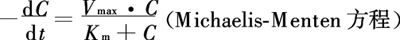
\includegraphics[width=\textwidth,height=\textheight,keepaspectratio]{./images/Image00045.jpg}
 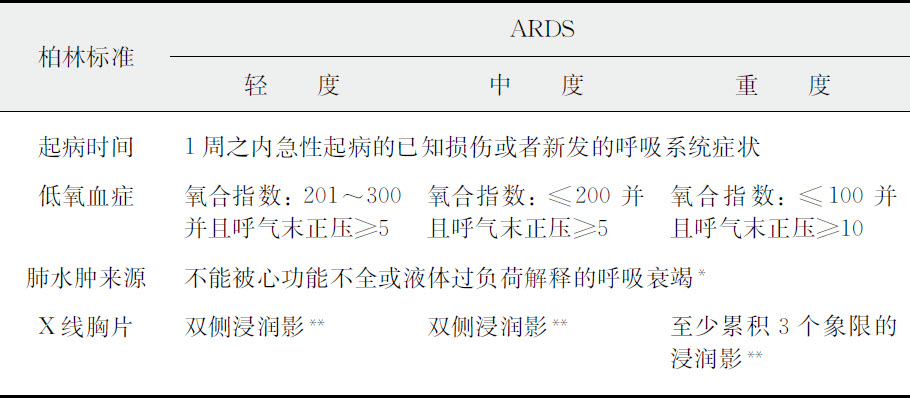
\includegraphics[width=\textwidth,height=\textheight,keepaspectratio]{./images/Image00046.jpg}
 \captionsetup{justification=centering}
 \caption{脑动静脉畸形\\{\small A~D为同一患者,平扫(A、B图)左侧颞叶有局灶性高、等混杂密度区,形态不规则,其边缘有蚯蚓状高密度影(引流静脉);增强扫描(C图)呈团块状强化,并见迂曲的引流静脉影;CTA(D图)清晰显示畸形血管团和粗大的引流静脉}}
 \label{fig2-27}
  \end{figure} 

其并发症有出血、梗死、软化灶及局限脑萎缩表现。

\textbf{【鉴别诊断】}
钙化明显的肿瘤以及强化明显的肿瘤(如胶质瘤)其水肿及占位效应均较显著,可与AVM鉴别。AVM增强扫描的时间-密度曲线与血管相似亦是与肿瘤鉴别的重要依据。

\subsection{颅内海绵状血管瘤}

本病占脑血管疾病的7%,近年来的研究显示其属不完全染色体显性遗传性疾病。目前多认为其发生源于脑内毛细血管水平的血管畸形,可位于脑内或脑外,为非真性肿瘤。

\textbf{【病理】}
病灶由微动脉延伸出来的、血流缓慢的、大小不等的丛状薄壁的血管窦样结构组成,其间有神经纤维分隔,窦间没有正常脑组织。由于其血管壁薄而缺乏弹性,且易于发生玻璃样变、纤维化,因而易出血,并可有胶质增生、坏死囊变、钙化,病灶可全部钙化形成“脑石”。病灶周围可见含铁血黄素沉着或有机化的血块。病灶无明显的供血动脉及引流静脉。

\textbf{【临床症状】}
好发于40~60岁,常以颅内出血为首发症状。典型表现为癫痫发作、突发性头痛和进行性神经功能障碍等。

\textbf{【CT表现】}
80%位于幕上,好发于额、颞叶,也可发生于蛛网膜下、硬膜下,脑外者多位于鞍旁海绵窦区。多表现为界限清楚的圆形或卵圆形的等至稍高密度影(图\ref{fig2-28})。其内可见“颗粒征”颇有特征,即在略高密度背景内含有数量不一的颗粒状高密度影和低密度影,前者为钙化,后者为血栓形成。除急性出血或较大病灶,灶周一般无水肿及占位征象。可能因为供血动脉太细或已有栓塞,也可能因病灶内血管床太大,血流缓慢使对比剂稀释,致使增强扫描不强化或仅见周边强化。其强化程度取决于病灶内血栓形成和钙化的程度,血栓形成轻、钙化不明显者强化明显。国外报道脑外者可有骨侵蚀。

\begin{figure}[!htbp]
 \centering
 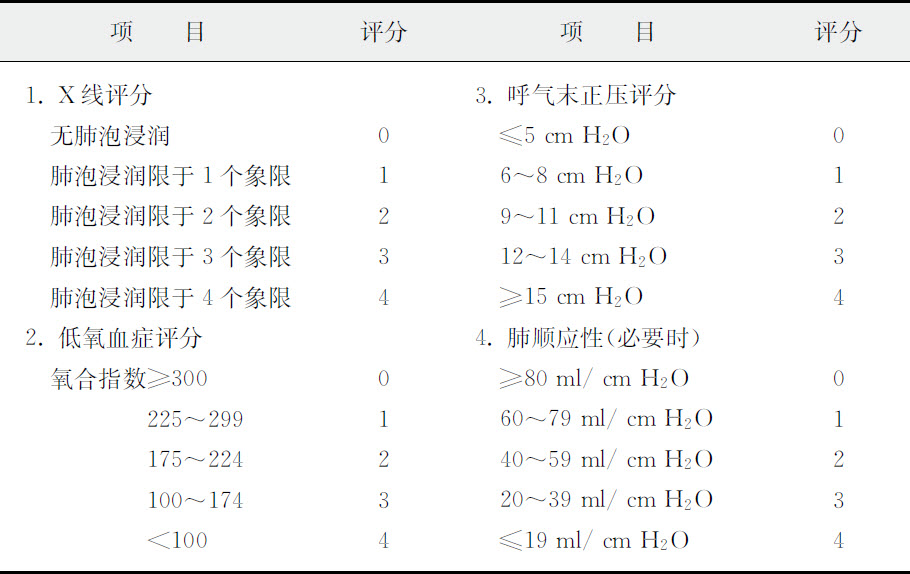
\includegraphics[width=.7\textwidth,height=\textheight,keepaspectratio]{./images/Image00047.jpg}
 \captionsetup{justification=centering}
 \caption{颅内海绵状血管瘤\\{\small A、B非同一患者,A示病灶位于小脑左侧半球,B示病灶位于脑干;病灶均呈近圆形稍高密度灶,周围无水肿}}
 \label{fig2-28}
  \end{figure} 

\textbf{【鉴别诊断】}
①主要应与脑膜瘤鉴别。后者平扫密度多均匀一致,增强扫描明显强化,常有明显占位征象,并可出现水肿征象及颅骨增生和吸收有助鉴别。②少数血管瘤呈环状并伴壁结节,偶有出血,病灶内显示血-液平面伴周围水肿,不易与胶质瘤等相鉴别。

\subsection{脑静脉性血管畸形}

本病又称脑静脉性血管瘤、脑发育性静脉异常,是一种组织学上由许多扩张的髓静脉和一条或多条引流静脉组成的血管畸形。国外有学者认为是一种正常引流静脉的非病理性变异。

\textbf{【病因病理】}
其病因不明,多认为是胚胎发育时宫内意外因素导致静脉阻塞,由侧支代偿所致。其形成时间在脑动脉形成之后,故仅含静脉成分。畸形血管由许多扩张的放射状排列的髓静脉汇入一条或多条引流静脉组成,向皮质表面和静脉窦或向室管膜下引流,可分为皮层表浅型、皮层下型和脑室旁型。

\textbf{【临床表现】}
好发于35~40岁,男女发病率相近。一般无症状,少数可产生癫痫、头痛,出血者可有感觉和运动障碍、共济失调等。

\textbf{【CT表现】}
它可发生在脑静脉系统的任何部位,但以额叶侧脑室前角附近的髓质区和小脑深部髓质区最常见,其次为顶叶、颞叶和脑干。

CT平扫阳性率不到50%。最常见的表现为圆形高密度影(34%),系扩张的髓静脉网,无水肿和占位效应,可见高密度的含铁血黄素沉着或钙化。

增强扫描阳性率为87%,可见3种表现:①白质中圆形强化影(32.5%),系髓静脉网或引流静脉;②穿越脑的线形增强影(32.5%),为引流静脉;③两者同时出现(18.6%)。

特征性表现是三维CT血管造影(CTA)静脉期脑静脉成像(CTV)出现“海蛇头”样的深部髓静脉汇集到单根粗大的引流静脉,然后汇入到表浅的表层静脉或硬膜窦等征象。但发生于脑室壁上者“海蛇头”征象不明显。

\subsection{Galen静脉瘤}

本病又称大脑大静脉扩张、大脑大静脉瘘、大脑大静脉畸形等。

\textbf{【病因病理】}
本病是由于动静脉短路,流入Galen静脉(即大脑大静脉)内的血流增多引起局部管腔扩张。这些短路血管多来源于颈内动脉系统或基底动脉系统,多异常扩大迂曲。静脉窦闭塞引起大脑大静脉回流受阻也是其重要的致病原因。压迫中脑导水管可致脑积水。

\textbf{【临床表现】}
在新生儿、幼儿中常因动脉血直接进入静脉造成心功能不全。脑积水后可出现头痛、痉挛性抽搐、颅内压增高等症状。

\textbf{【CT表现】}
平扫可见第三脑室后部中线处之大脑大静脉池区等密度或高密度的圆形肿块,病灶边缘多光滑,与窦汇之间有扩张的直窦相连为特异性表现。可伴有病灶边缘钙化、局部脑萎缩、血肿或脑积水。增强扫描病灶呈均匀性强化,偶可显示强化的供血动脉和引流静脉。

\subsection{颈动脉海绵窦瘘}

本病是指颈动脉及其分支与海绵窦之间异常沟通所致的一组临床综合征。海绵窦为中颅凹两层硬脑膜构成的硬脑膜窦,眼上静脉、眼下静脉、蝶顶窦静脉、外侧裂静脉和基底静脉汇入其中,颈动脉穿行其间。这是体内惟一动脉通过静脉的结构。当任何原因造成颈内动脉壁破裂后,动脉血直接流入海绵窦,就形成海绵窦区动静脉瘘。

\textbf{【病因】}
病因分为两大类:①外伤性:多见,大多由颅底骨折所致;②自发性:病因较多,主要见于颈内动脉虹吸部动脉瘤破裂、硬膜型动静脉畸形及遗传性胶原纤维缺乏病等。此外,动脉硬化、炎症、妊娠等也可造成自发性。根据解剖部位分为颈动脉海绵窦瘘和硬脑膜动脉海绵窦瘘,前者多为外伤性,后者多为自发性。

\textbf{【临床表现】}
头痛、癫痫、耳鸣、视力障碍、搏动性突眼、眼球运动障碍、颅内杂音,甚至因颅内出血而出现相应症状。

\textbf{【CT表现】}
①患侧海绵窦扩大,密度增高;②眼上静脉增粗;③眼球突出;④增强示扩大的海绵窦及迂曲的眼上静脉显著强化(图\ref{fig3-8},见第三章)。此外,眼外肌肥厚和眶内软组织肿胀、突眼,患侧脑组织水肿、出血、萎缩是引流静脉压力增高及“盗血”引起的继发改变。

\subsection{颅骨膜血窦}

本病又称血囊肿、局限性静脉曲张或骨血管瘤,是指紧贴颅骨外板的扩张静脉,它们穿过颅骨的板障静脉与硬膜窦相交通。

\textbf{【病因】}
其原因不明,可由先天性、自发性或外伤性所致。有学者认为外伤是本病的最主要因素。

\textbf{【临床表现】}
多见于儿童,通常以头皮肿块就诊。头皮中质软的膨隆性肿块,无搏动,局部皮肤可以微红或青紫色。通常位于中线部位,偶尔位于侧旁,以额部为主,偶有头痛、恶心、乏力等。肿块随颅内压力的变化而改变其大小,即平卧或头低时肿块增大为其特征性症状。

\textbf{【CT表现】}
大多位于颅外中线部位或附近,上矢状窦近端,以额、顶部多见。表现为颅外头皮下均匀的软组织密度肿块,边缘清晰,无钙化,随体位大小可变化。颅外板可有轻度压迹,颅骨内有孔状骨质缺损。增强扫描静脉窦内对比剂可通过颅骨的缺损弥散至囊腔内,呈均匀或不均匀显著强化。

\subsection{颅内血管延长症}

本病是指颈内动脉及椎基底动脉有规律的直径增大和普遍而有规律的延长为特征的血管异常。颈内动脉及椎基动脉的延长属于一种少见的先天性血管壁异常。

\textbf{【病理】}
延长的血管均伴有不同程度的动脉粥样硬化、弹性内膜的破坏及其肌壁的纤维化,最终导致血栓形成或栓塞。

\textbf{【临床表现】}
其发病特点主要取决于受累血管的范围、病变大小及所压迫的邻近组织情况。基本分为3类:①脑血管意外;②颅神经受压症状:如Ⅲ、Ⅴ~Ⅷ颅神经受压;③占位效应对脑组织功能的影响:如痴呆、共济失调、震颤麻痹等,也有阻塞性脑积水的可能。

\textbf{【CT表现】}
本病所涉及的血管有基底动脉、颈内动脉幕上段、大脑中动脉、大脑后动脉。CTA可发现异常扭曲扩张的颈内或基底动脉段,管壁可钙化。其中,基底动脉病变的诊断标准为上段基底动脉的直径增大达4.5mm和基底动脉上段超过床突平面6mm以上,且延长的血管可伴有迂曲移位和血管袢形成。

\subsection{烟雾病}

本病又称Moyamoya病、脑底动脉环闭塞、脑底异常血管网症等,是一种脑动脉进行性狭窄、闭塞性疾病。

\textbf{【病因】}
其病因不明,凡能引起颈内动脉末端、大脑前动脉和大脑中动脉近端慢性进行性闭塞的先天因素(发育不良)或后天因素(外伤、感染、动脉硬化)均可导致本病。近来遗传因素受到重视。

\textbf{【临床表现】}
以10岁以前儿童多见,亦可见于成人。主要有缺血性和出血性两大类表现。脑血管造影是确诊的主要手段。

\textbf{【血管造影】}
特点为:①大脑前、中动脉起始处狭窄或闭塞;②脑底异常血管网形成;③侧支循环广泛建立;④两侧颞、额、顶叶、基底节区梗死或出血。本病即因造影时异常血管网和侧支循环的显影似烟雾状而得名。

\textbf{【CT表现】}
无特异性。①脑梗死、软化灶:常见于颞、额、顶叶,很少见于基底节,小脑、脑干不发生。②脑萎缩:多为双侧性,额叶为甚,脑室扩大以侧脑室和第三脑室显著。③出血灶:可为脑内或蛛网膜下腔。④颅底、基底节区有点状、迂曲、不规则的网状影,并可见强化。

\section{颅脑外伤及其他损害}

\subsection{头皮损伤}

颅盖软组织在额、顶、枕部分为皮肤、皮下组织、帽状腱膜、帽状腱膜下层和颅骨骨膜5层。前3层紧密连接CT不能识别。帽状腱膜下层由疏松结缔组织构成,内含少量血管,CT呈低密度带。而在颞部则由皮肤、皮下组织、颞浅筋膜、颞深筋膜、颞肌和颅骨骨膜6层构成。

头皮损伤包括:①头皮血肿或称颅外血肿,包括位于头皮与帽状腱膜间的皮下血肿、帽状腱膜下血肿(图\ref{fig2-29})和骨膜下血肿;②头皮撕裂伤、擦伤和挫伤等。

\begin{figure}[!htbp]
 \centering
 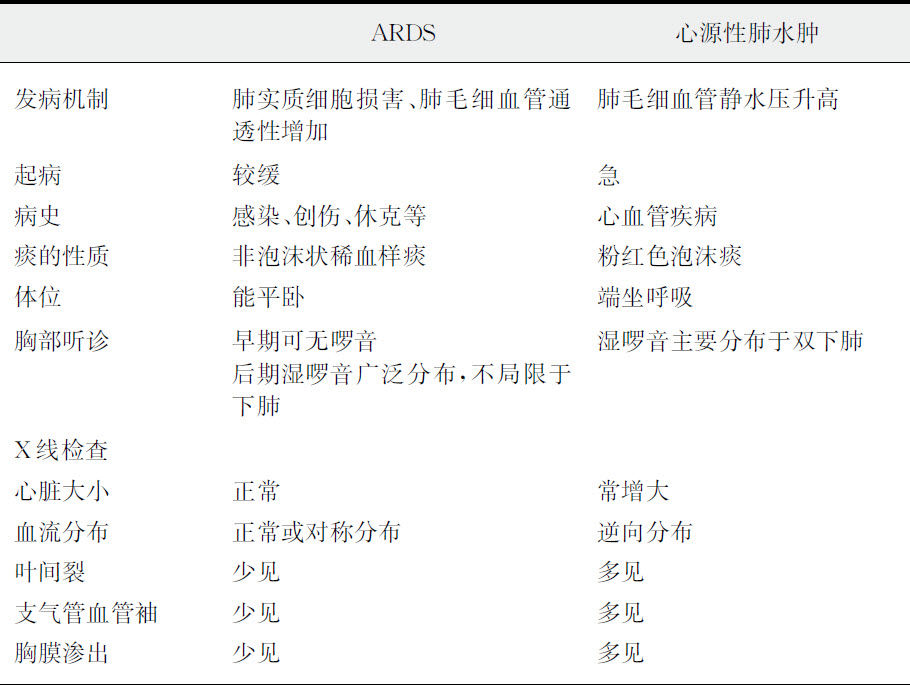
\includegraphics[width=.7\textwidth,height=\textheight,keepaspectratio]{./images/Image00048.jpg}
 \captionsetup{justification=centering}
 \caption{帽状腱膜下血肿\\{\small 出血位于左侧额顶枕部帽状腱膜下}}
 \label{fig2-29}
  \end{figure} 

头皮血肿多由于头皮血管破裂引起,也可因板障静脉或硬脑膜血管破裂,血液沿骨折缝聚集于骨膜下,后者多伴硬膜外血肿。

\subsection{颅骨骨膜下血肿}

骨膜下血肿是颅外血肿的少见类型。

\textbf{【病因病理】}
多发生于新生儿产伤和婴幼儿头部外伤。血肿位于颅骨外板与对应的骨膜之间的潜在腔隙,好发于顶骨,其次为枕骨。

\textbf{【临床表现】}
产伤所致者几乎均因头皮下出现软组织包块,未消散且逐渐变硬而就诊。

\textbf{【CT表现】}
特征性表现是新鲜血肿范围达到受累骨的整个表面,中止于颅缝或不跨越颅缝,边缘清楚锐利。而头皮下及帽状腱膜下血肿不受颅缝限制有助于鉴别。2~3周后血肿包膜出现弧形、壳状钙化,从边缘开始逐渐形成一个完整的包壳,这一过程大约需要3~6个月。与此同时血肿逐渐吸收机化,血肿完全机化约需1年,此时血肿包膜钙化或骨化形似颅骨外板,血肿机化钙化形似板障。再经过长期的塑形与颅骨融合,致局部颅骨增厚、外突隆起,并可成为永久性后遗表现。

此外,少数在血肿部位出现或大或小的囊状骨缺损,可持续数年或更久。与颅骨表皮样囊肿、嗜酸性肉芽肿、韩雪柯氏病相类似,应注意鉴别。

\subsection{颅骨骨折}

1.按骨折形态分类:①线状骨折。②凹陷骨折:婴幼儿颅骨质软,骨折部位凹陷,但不出现骨折线,称为乒乓球样凹陷骨折。③粉碎性骨折:大多数凹陷骨折被分离为多个骨碎块,则被称为粉碎性骨折。④穿通骨折:多为锐器直接损伤,少数为火器伤。局部头皮全层裂伤,可有各种类型骨折,还可见颅内血肿、异物及脑损伤。⑤颅缝分离:两侧不对称或颅缝宽>2mm。

2.按骨折部位分类:①颅盖骨骨折。②颅底骨折。

3.诊断骨折应注意的问题:①颅骨血管沟:仅有内板压迹,边缘为硬化边。②板障静脉:常不规则,可见于对侧,并终端于静脉湖。③颅骨缝:特有的部位及走行,是区别骨折线的标志。④是否有颅内积气:积气可见于蛛网膜下腔、脑室系统、硬膜下腔,以及硬膜外血肿内,甚至脑实质内。

\subsection{硬脑膜外血肿}

硬脑膜紧贴颅骨内板,当颅骨骨折或脑膜血管破裂、出血使其与颅内板分离时则形成硬膜外血肿。

\textbf{【病理】} 多发生于头颅直接损伤的部位。约
95%伴颅骨骨折,70%~80%病例因骨折所致脑膜中动脉及其分支断裂,少数因骨折伤及板障静脉、静脉窦和蛛网膜粒。血肿可单发或多发,呈凸透镜形,多不伴有脑实质损伤。

\textbf{【临床表现】}
伤后有短时原发昏迷,清醒后头痛、呕吐逐渐加重并再度昏迷。清醒时间的长短,由出血量多少和出血速度决定。重者如不及时处理,可形成脑疝。

\textbf{【CT表现】}
因硬膜与颅骨紧密相连,故血肿局限呈梭形高密度,CT值为50~70Hu。血肿的脑侧缘光滑(图\ref{fig2-30}),好发于骨折处。由于硬膜在颅缝处与骨结合紧密,故血肿不超越颅缝。但骨折如跨越颅缝,则血肿亦可跨越颅缝,也可从幕上延及幕下或跨越中线。血肿有占位效应,但较硬膜下血肿轻,多不伴脑实质损伤,但压迫邻近血管时可发生脑水肿或脑梗死。少数受伤时无症状,以后才发生慢性硬膜外血肿。慢性硬膜外血肿其壁机化增厚并可钙化。

\begin{figure}[!htbp]
 \centering
 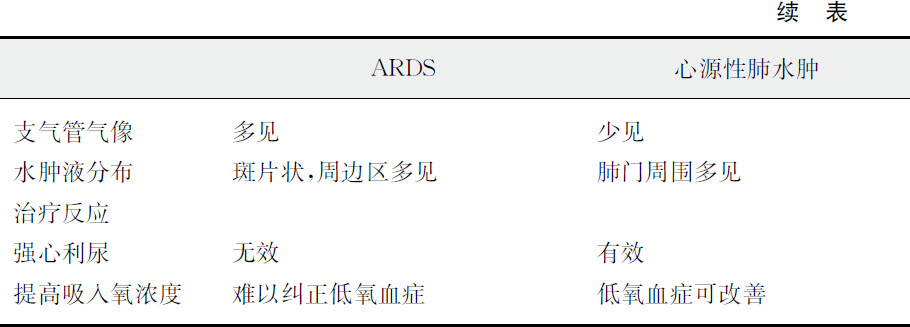
\includegraphics[width=.7\textwidth,height=\textheight,keepaspectratio]{./images/Image00049.jpg}
 \captionsetup{justification=centering}
 \caption{硬膜外血肿\\{\small 右侧颅骨内板下有梭形高密度区,边缘清晰锐利}}
 \label{fig2-30}
  \end{figure} 

\subsection{硬脑膜下血肿}

硬膜下血肿位于硬膜和蛛网膜之间,多因减速性挫伤(对冲伤)所致,无颅骨骨折或骨折仅位于暴力部位。

\textbf{【病理】}
其血源多为脑对冲伤处的静脉、小动脉或由大脑向上矢状窦汇入的桥静脉撕裂所致。呈新月形包绕在大脑表面,在伤后不同时间形态变化各异,约50%合并脑挫裂伤。临床、病理和影像均分为急性、亚急性和慢性3期。

CT上等密度硬膜下血肿占硬膜下血肿的16%。据有关文献报道,多发生在初次损伤后30~90天,亦有报道可达120天,甚至150余天。等密度硬膜下血肿的原因为:①血肿由高密度向低密度发展过程中血肿密度与脑组织密度相近时;②偶有低蛋白血症(如贫血)病人的急性期血肿呈等密度;③再出血或慢性出血进入到慢性硬膜下血肿,而形成等密度慢性硬膜下血肿。

\textbf{【临床表现】}
急性者病情多较重,且发展迅速,出现中间清醒期或意识好转期者较少,颅内压增高、脑受压和脑疝症状出现早。慢性硬膜下血肿患者年龄常较大,只有轻微外伤史,在伤后数周或数月出现颅内压增高症状,呈慢性过程。

\textbf{【CT表现】}

\subsubsection{三期表现}

1.急性期:伤后3天内。一般呈均匀高密度的新月形(图\ref{fig2-31}A),血肿可跨颅缝,但不超过中线。占位效应著,常伴脑挫裂伤,可形成脑疝。有3种非典型表现:①血肿密度不均:可能与急性出血还未凝固、凝血早期血清外溢或蛛网膜破裂脑脊液进入硬膜下有关;②血肿呈梭形表现:可能与出血没有及时散开有关;③血肿同侧侧脑室扩大:可能与同侧室间孔被迅速挤压梗阻所致。

此外,多不伴骨折,但骨折后硬膜撕裂也可形成急性硬膜下血肿。

2.亚急性期:伤后4天~3周内。血肿可逐渐变为等密度,而表现为皮质区均匀受压,脑沟消失,灰白质交界处被均匀向内推移。但双侧均有血肿,中线推移可不著。亚急性血肿的较早期出现细胞沉淀效应可出现密度上低下高的液体界面。

3.慢性期:伤3周后。此时血肿包膜形成,凝血块液化,逐渐变成液性低密度(图\ref{fig2-31}B),血肿壁机化增厚或钙化。血肿内肉芽组织增生、机化形成包膜,故可见慢性硬膜下血肿有分隔表现。

\subsubsection{等密度硬膜下血肿}

平扫表现为中线结构及脑室受压移位、变形,脑沟、裂池变窄消失、灰白质界面内移等,均属间接征象(图\ref{fig2-31}C)。增强扫描可显示血肿的位置、大小、形态而确诊。



\begin{figure}[!htbp]
 \centering
 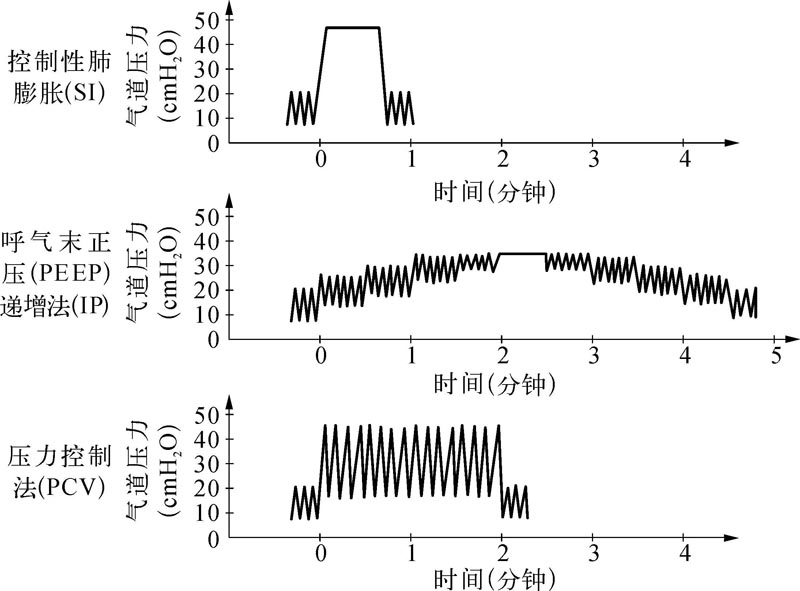
\includegraphics[width=.7\textwidth,height=\textheight,keepaspectratio]{./images/Image00050.jpg}
 \includegraphics[width=.7\textwidth,height=\textheight,keepaspectratio]{./images/Image00051.jpg}
 \captionsetup{justification=centering}
 \caption{硬膜下血肿\\{\small A.急性期硬膜下血肿,病灶位于左侧额顶骨内板下;B.慢性期硬膜下血肿,病灶位于左侧额顶枕骨内板下,有密度上低下高的液体界面;C.慢性等密度硬膜下血肿,病灶位于左侧额顶枕骨内板下和右侧额部}}
 \label{fig2-31}
  \end{figure} 

\subsection{特殊部位的硬脑膜下血肿}

特殊部位的硬膜下血肿主要指大脑镰、小脑幕硬膜下血肿。

\textbf{【病因病理】}
其受力方式可以是加速运动或减速运动的直接作用力,也可以是引起大脑镰、小脑幕严重移位的内在推力。目前,普遍认为是该处的桥静脉与静脉窦连接部撕裂,血液进入硬膜下腔所致。

\textbf{【CT表现】}

1.大脑镰硬膜下血肿:正常大脑镰宽为<3mm,硬膜下血肿表现为大脑纵裂呈带状增宽,密度增高,宽为3~12mm,CT值达68~85Hu,可有占位效应。硬膜侧有坚硬的硬膜阻挡,故其内缘平直而光整;外缘因蛛网膜的张力低和脑沟、脑回的阻力不均衡呈局限的弧形或波浪状。但与脑沟不通为其特点,并可依此与蛛网膜下腔出血相鉴别(图\ref{fig2-32}A、B)。

2.小脑幕硬膜下血肿:呈扇形、片状、新月形等形状的高密度,内缘止于小脑幕切迹处。边缘光滑锐利,占位效应不著(图\ref{fig2-32}C、D)。由于小脑幕凹面向下,横断扫描像一般显示:血肿位于小脑幕上者,其内侧缘清晰,外侧缘模糊;位于小脑幕下者反之。



\begin{figure}[!htbp]
 \centering
 \includegraphics[width=\textwidth,height=\textheight,keepaspectratio]{./images/Image00052.jpg}
 \includegraphics[width=\textwidth,height=\textheight,keepaspectratio]{./images/Image00053.jpg}
 \captionsetup{justification=centering}
 \caption{特殊部位硬膜下血肿\\{\small A~D为同一患者;A、B血肿位于大脑镰旁,大脑纵裂呈带状增宽,边缘清晰、平直而光整;C、D血肿位于右侧小脑幕处,呈扇形高密度,内缘止于小脑幕切迹处,边缘光滑锐利}}
 \label{fig2-32}
  \end{figure} 

以上两者均可因部分容积效应或同时合并该区域的蛛网膜下腔出血而使血肿边界不清。

\textbf{【鉴别诊断】}
大脑镰旁和小脑幕处的硬膜下血肿主要应与蛛网膜下腔出血相鉴别。①前者边界光整清楚;后者则模糊不规则,因向脑沟延伸而多呈羽毛状,常波及相邻脑池和脑室。②前者大脑镰部占位效应常见;后者较少见。③前者血肿不能触及胼胝体膝部;后者可紧贴。④前者急性期密度多为55~75Hu,多在2周后吸收或变为低密度;后者CT值多在55Hu以下,且多在1周内(甚至24h)消失。⑤采用薄层扫描,特别冠状和矢状面重建可较清楚显示血肿的形态和解剖位置。此外,脑膜钙化CT值明显高于血肿可资鉴别。

\subsection{硬脑膜下积液}

本病又称硬膜下水瘤,是指硬膜下只含有脑脊液成分。

\textbf{【病因病理】}
它是由于外伤后蛛网膜破裂,脑脊液流入硬膜下所造成的,并多认为其形成机制是蛛网膜破口的活瓣效应的结果。常在外伤后几周内产生,少数因伴有慢性渗血而转化为慢性硬膜下血肿。

\textbf{【临床表现】}
多见于老年人及儿童。急性者(伤后72小时内)与急性颅内血肿症状相似,主要表现为头痛、恶心、呕吐等颅内压增高症状,亦可有局部脑受压症状。慢性者(3周后)可见嗜睡、朦胧、定向力差、精神障碍。

\textbf{【CT表现】}
多位于额、颞部,老年人双侧多见。呈颅骨内板下新月形水样密度区,因受压脑沟变浅、脑回变平(图\ref{fig2-33})。少数经复查液体密度增高,而转化为等密度或稍低密度慢性硬膜下血肿。

\begin{figure}[!htbp]
 \centering
 \includegraphics[width=.7\textwidth,height=\textheight,keepaspectratio]{./images/Image00054.jpg}
 \captionsetup{justification=centering}
 \caption{硬膜下积液\\{\small 双侧额颞骨内板下新月形水样密度区,脑沟变浅、脑回变平}}
 \label{fig2-33}
  \end{figure} 

\textbf{【鉴别诊断】}
①慢性硬膜下血肿:有人认为硬膜下血肿吸收后也可称为硬膜下积液。但慢性血肿CT值偏高,包膜有强化,常呈梭形,可予鉴别。②脑萎缩:脑沟裂增深、增宽,甚至脑室扩大等有别于硬膜下积液之脑沟、回变浅平。

\subsection{外伤性蛛网膜下腔出血}

\textbf{【病因病理】}
出血来源于外伤后软脑膜和皮层血管的断裂、脑挫裂伤的渗血及脑内血肿破入。单独蛛网膜下腔出血少见,多伴脑挫裂伤。

\textbf{【临床表现】}
因脑膜刺激引起剧烈头痛、恶心呕吐,查体可发现颈强直、Kernig征阳性。

\textbf{【CT表现】}
高密度血液充填于脑表面脑沟中或脑裂、脑池中。吸收消散快,长者1周,短者1~2天,最快可达10小时左右。可伴脑挫裂伤的水肿、出血等表现。

此外,少数(包括自发性)出血点因远离宽大的脑池、脑裂,而且出血较快,局限于局部颅骨内板下,与硬膜下血肿相似,但其内缘不锐利、密度较低且不均匀,且短期内能快速吸收。

\subsection{外伤性脑室内出血}

本病是一种较少见的重型脑损伤,预后差,死亡率高。

\textbf{【病因病理】}
本病可分为两类:①原发性:为外伤致脑室内血管破裂出血;②继发性:为脑内血肿破入脑室。其发生机理有以下几种学说:①脑外伤瞬间,外力(尤其矢状方向外力)使脑室扩大变形,撕裂室管膜下血管引起脑室出血。②弥漫性轴索损伤,由于剪切力的作用脑室壁破裂,引起室管膜下血管损伤出血。③室管膜下潜在的畸形血管破裂出血。④凝血功能障碍,外伤作为诱因。⑤脑内血肿破入脑室。

\textbf{【临床表现】}
多伴有其他类型的脑损伤,故缺乏特征性。可有以下表现:①意识障碍;②脑膜刺激征:脑室内出血流入蛛网膜下腔所致;③体温升高:是血性脑脊液的吸收热,并与出血刺激丘脑下部体温调节中枢有关。伴有其他部位的损伤时有相应表现和体征。

\textbf{【CT表现】}
少量出血时多沉积在侧脑室后角、第三脑室后部或第四脑室顶部,大量出血常呈脑室“铸型”样表现。早期可有分层现象,以后呈等或低密度。可并发不同程度的阻塞性脑积水,多合并其他类型脑损伤。

\subsection{脑挫裂伤}

脑组织外伤后发生水肿、静脉淤血、渗血及毛细血管的散在点状出血,病理上称为脑挫伤;而当软脑膜和脑组织及其血管断裂时称为脑裂伤。因而两者多合并存在,且临床和影像检查难以区分,故统称为脑挫裂伤。

\textbf{【病因病理】}
直接打击的外力可造成受力处的脑挫裂伤,此种较少。多由于运动中的撞击造成的对冲伤引起。病理改变有局部脑水肿,静脉淤血、渗血及毛细血管的散在点状出血,严重者出血较多,形成脑内血肿,还可有坏死液化等改变。

\textbf{【临床表现】}
都有意识丧失,出现一过性昏迷,重者持续昏迷。患者有头痛、呕吐等颅内压升高或脑膜刺激征。损伤部位不同可出现偏瘫、偏盲、肢体张力和腱反射的异常。

\textbf{【CT表现】}

1.常见表现:①局部脑组织呈低密度水肿,界限不清,多位于皮层区。水肿区内有一处或多处点片状出血灶称为灶状出血。②一处或多处脑内血肿(出血灶>2cm称为血肿),形态边缘不规整(图\ref{fig2-34})。血肿周围有不同程度水肿和占位效应。③灶状出血及小血肿可在数小时内扩大融合,并可引起脑疝如镰下疝、天幕疝等。

\begin{figure}[!htbp]
 \centering
 \includegraphics[width=.7\textwidth,height=\textheight,keepaspectratio]{./images/Image00055.jpg}
 \captionsetup{justification=centering}
 \caption{脑挫裂伤\\{\small 双侧额颞叶有许多斑片状不规则出血灶,鞍上池、四叠体池内有积血}}
 \label{fig2-34}
  \end{figure} 

2.外伤性迟发性脑内血肿:伤后首诊CT扫描未发现血肿,相隔数小时、数天复查或手术发现有新的血肿者称为外伤性迟发性脑内血肿。属于原发性脑损伤,可发生于伤后1.5小时至数天,90%以上出现在伤后24~48小时,也有报道多见于3日至1周内。此外,颅脑损伤的迟发性表现还有脑挫裂伤、硬膜外血肿、硬膜下血肿、蛛网膜下腔出血、脑水肿等。

3.其他伴发的外伤性颅内病变:硬膜外或硬膜下血肿、蛛网膜下腔出血、弥漫性脑水肿、硬膜下积液、DAI等。

\subsection{脑干损伤}

脑干损伤较少,多合并大脑半球的弥漫性损伤。

\textbf{【病理】}
本病可分为原发性和继发性。原发性病理改变有脑干震荡、挫裂伤、出血、软化和水肿。有人把其分为4类:①弥漫性轴索损伤(DAI);②原发性多发斑点状出血;③桥脑、延髓撕裂;④直接表浅撕裂或挫伤。其中以DAI最常见,且多为非出血性。继发性脑干损伤是由颅内血肿、脑水肿所致的天幕裂孔疝压迫脑干并使脑干血管受牵拉,进而导致脑干缺血和出血。

\textbf{【临床表现】}
病情严重,常见表现有意识障碍、去大脑强直、肌张力增高和眼球位置异常。患者常见双侧瞳孔缩小。

\textbf{【CT表现】}
因受后颅窝伪影干扰和分辨率限制对非出血性脑干损伤诊断困难。①原发性:常表现为局部脑池消失,亦可显示小灶状出血。②继发性:可见出血、梗死,并可见幕上血肿、弥漫性脑肿胀、弥漫性脑水肿、天幕裂孔疝和脑干受压移位等表现。

\subsection{弥漫性脑损伤}

弥漫性脑损伤包括弥漫性脑水肿、弥漫性脑肿胀和弥漫性轴索损伤(DAI)。弥漫性轴索损伤有文献也称为弥漫性脑白质损伤。

\textbf{【病因病理】}
DAI是因外伤造成的剪切力(旋转暴力)作用于脑灰白质交界处、大脑深部结构和脑干区,导致神经轴索的广泛挫伤、断裂及脑组织小灶出血、水肿。

脑水肿和脑肿胀的病理改变分别为细胞外液和细胞内液增多。两者常同时存在,很难区分和鉴别,因此统称为脑水肿(脑组织液体含量增多引起的脑容积增大和重量增加)。

\textbf{【临床表现】}
脑水肿和脑肿胀轻者无明显症状和体征,重者出现头痛、头晕、呕吐等颅内高压征;可出现半身轻瘫和锥体束征;严重者可发生脑疝,以至死亡。

DAI因广泛轴索损伤使皮层及皮层下中枢失去联系而致伤后即刻意识丧失,多持久昏迷,甚至处于植物人状态,死亡率高。

\textbf{【影像学表现】}

1.弥漫性脑水肿和(或)脑肿胀:CT表现为低密度,密度低于邻近脑白质,CT值多<20Hu。两侧弥漫性病变可致脑室普遍受压变小,重者可致脑室、脑沟和脑池消失。

2.DAI的诊断标准:①受伤机制:受伤时头部处于运动状态,由旋转暴力所致。②临床表现:伤后有原发性昏迷伴躁动不安,无明确神经定位体征,亦无窒息及低血压等脑缺氧情况。③CT表现:脑组织弥漫性肿胀(灰白质密度普遍降低,但其密度减低不及脑水肿),灰白质分界不清,其交界处有散在斑点状出血灶(<2cm),伴有蛛网膜下腔出血。脑室、脑池受压变小,无局部占位征象。④MR表现:脑肿胀、脑室脑池因受压而减小或闭塞,脑白质及胼胝体、脑干、小脑可见点状、片状或散在小出血灶(<2cm),中线结构无明显移位。⑤合并症:可合并其他颅脑损伤,如蛛网膜下腔出血、脑室出血、硬膜下及硬膜外血肿及颅骨骨折等。

DAT的分期:目前有学者将DAI分为3期。Ⅰ期:较轻,损伤仅见脑叶白质,常见于额、颞叶。Ⅱ期:损伤较重,胼胝体出现病灶。Ⅲ期:严重损伤,脑干出现病灶。

总之,因DAI有80%为非出血性病灶,仅20%有小的中心出血,故CT难以发现。其CT检出率不到30%,而MR可高达90%。

\subsection{外伤性脑疝}

\subsubsection{天幕疝}

分为3型:①颞叶型:常为单侧,占位效应显著,颞叶组织(钩回、海马回)疝入幕下;②中央型:常为双侧颅内压升高,脑干向下移位而不向一侧移位,双侧外侧裂池、环池变窄或消失;③小脑型:幕下压力升高,脑干和(或)小脑上移,环池及枕大池狭窄或消失,第三脑室后部上抬。

颞叶天幕疝的诊断标准:①颅内压增高征象:中线结构明显移位,患侧环池增宽,除环池外的基底池(如四叠体池、鞍上池)及侧裂池浅小甚至闭塞;②颞叶伸至幕下≥3.0mm,但必须存在上述同侧颅内压增高征象,<3.0mm为可疑。同时可见脑干受压变形、病侧环池增宽;③如无颅内压增高征象存在,颞叶轻度下移,应视为正常变异。

此外,斜坡垂直线的扫描法有助于显示疝入幕下的与颞叶相连的脑组织,并进而结合脑干、脑池之形态与正常小脑组织相鉴别。

\subsubsection{镰下疝}

表现为扣带回和大脑前动脉移向对侧,较硬的大脑镰一般移位不著。侧脑室前角受压变窄(图\ref{fig2-35})。

\begin{figure}[!htbp]
 \centering
 \includegraphics[width=.7\textwidth,height=\textheight,keepaspectratio]{./images/Image00056.jpg}
 \captionsetup{justification=centering}
 \caption{镰下疝\\{\small 右侧颞额顶部硬膜下血肿及局部脑沟内有血液充填,右侧额叶脑组织经大脑镰下跨越中线移向左侧}}
 \label{fig2-35}
  \end{figure} 

此外,还可见脑组织通过缺损颅骨外疝、小脑扁桃体疝(枕骨大孔疝)。

\subsection{外伤性脑梗死}

外伤性脑梗死常发生在外伤后1周内。

\textbf{【病理机制】}
其发病机理大致归纳为以下几方面:①血管壁发生直接机械性损伤造成器质性狭窄或闭塞,致供血中断;②血管壁损伤引起局部脑血管痉挛,血液微循环发生障碍,致脑组织供血不全;③血管内皮损伤激活内源性、外源性凝血系统,促使血栓形成;④外伤后血管痉挛与血液流变学发生变化,脑血管反应性降低,脑血流量减少,引起血中自由基反应增强,造成细胞内环境紊乱,从而加重脑缺氧、坏死、溶解,导致脑梗死;⑤脑挫裂伤、蛛网膜下腔出血以及脑血肿、水肿等可使脑血管扭曲、痉挛收缩,加重原有的缺血、缺氧,导致脑梗死。此外,外伤后无明显症状的情况下,可发生腔隙性脑梗死,可能也与外伤后神经调节功能紊乱所致的脑血管痉挛有关。

\textbf{【CT分型】}
国内有学者将其分为5型:①腔隙性:多见于幼儿和儿童,呈卵圆形或裂隙状;②单脑叶型(或局灶型):多位于一侧脑叶或脑叶交界区,呈楔形或不规则形(图\ref{fig2-36});③多脑叶型(大面积型):是指2个以上脑叶的梗死;④挫伤出血型(混合型):表现为沿血管走向分布的低密度,多有规则边界,而脑挫伤低密度比梗死出现早,且密度不均、形态不规则,出血呈高密度,脑肿胀密度轻微减低、界限不清、双侧半球受累为其特点;⑤小脑与脑干型梗死。

\begin{figure}[!htbp]
 \centering
 \includegraphics[width=.7\textwidth,height=\textheight,keepaspectratio]{./images/Image00057.jpg}
 \captionsetup{justification=centering}
 \caption{外伤性脑梗死\\{\small A、B为同一患者,左侧颞部有硬膜外血肿,左侧枕叶呈大片状低密度,密度均匀、边缘平直}}
 \label{fig2-36}
  \end{figure} 

\subsection{脑外伤的并发症和后遗症}

1.并发症:①感染;②梗死;③脑膨出;④颈内动脉海绵窦瘘等。

2.后遗症:轻度挫裂伤可完全恢复正常而无后遗症。常见后遗症有:①脑软化;②脑萎缩;③脑穿通畸形(图\ref{fig2-37});④脑积水(交通性或阻塞性);⑤蛛网膜囊肿等。

\begin{figure}[!htbp]
 \centering
 \includegraphics[width=.7\textwidth,height=\textheight,keepaspectratio]{./images/Image00058.jpg}
 \captionsetup{justification=centering}
 \caption{右侧额叶脑穿通畸形\\{\small 脑挫裂伤1年后复查,右侧额叶水样密度灶,有张力,并与右侧脑室额角相通连}}
 \label{fig2-37}
  \end{figure} 

\subsection{放射性脑病}

本病是一种由各种原因放疗所致的脑组织放射性反应综合征。

\textbf{【病理】}
放射性损伤急性期和早期常表现为放射性诱导的脑水肿,晚期则主要以放射性坏死为主要特征。光镜观察有以下特征:①凝固性坏死;②脱髓鞘;③巨噬细胞反应;④血管周围细胞浸润;⑤血管纤维素样坏死、栓塞、玻璃样变或纤维素样变;⑥神经胶质增生;⑦无细胞性纤维化。

\textbf{【临床分期】}
国外有学者根据放疗后症状出现的时间分为3期:①急性期:多发生于放疗后几天至2周内,为血管源性水肿所致的颅内压增高,激素治疗有效;②早期迟发反应期:多发生于放疗后几周至3个月,大多数较短暂,预后较好;③晚期迟发反应期:多发生于放疗后几个月至10年或10年以上,该期主要病理改变为局限性放射性坏死、弥漫性脑白质损伤、大动脉损伤钙化性血管病及脑萎缩等不可逆性损害,局限性坏死和弥漫性脑白质损伤可分别或同时发生。

\textbf{【临床表现】}
①颅内压增高表现;②癫痫大发作;③局限性神经功能损害表现,如视障碍、同向偏盲、复视、失语、单侧运动和感觉障碍;④其他:头昏、嗜睡、反应迟钝、记忆力减退等,也有诱发脑膜瘤、纤维肉瘤、胶质瘤等脑肿瘤的报道。

\textbf{【CT表现】}
①急性期及早期迟发反应期:广泛性非特异性低密度水肿区,增强无强化,短期随访病灶消失。②局限性放射性坏死:病灶呈低密度,CT值约17Hu。灶周水肿明显,可见坏死、出血。增强扫描病灶多无强化,少数呈环形、片状、地图样不均匀强化。③弥漫性脑白质损伤早期:平扫可见脑室周围及半卵圆中心广泛低密度区。增强后多无强化,少数可见不均匀强化,提示有白质坏死存在。④弥漫性脑白质损伤晚期:可见钙化性微血管病和脑萎缩。前者可见多发钙化(占25%~30%),常见于基底节区,有时可见于皮层。弥漫性脑白质损伤一般在放疗早期出现,可持续几个月甚至几年。

\subsection{有机磷农药中毒的脑部损害}

有机磷农药中毒时主要毒性作用是抑制神经系统的乙酰胆碱酯酶,导致所有胆碱能神经传导部位的神经递质---乙酰胆碱的蓄积,引起中毒效应。

\textbf{【病理】}
其脑部损害的机制存在多种学说,但可以肯定的是有机磷中毒可损害脑部引起急性中毒性脑病,出现脑肿胀、水肿的病理改变。还有学者认为,有机磷中毒可使脑微血管内皮细胞和基底膜损伤,致通透性升高、毛细血管壁损伤而发生漏出性出血。此外,也可由于呼吸衰竭等原因而使脑组织缺血缺氧发生脑萎缩。

\textbf{【临床表现】}
毒蕈碱样症状、烟碱样症状和中枢神经系统症状。中枢神经系统症状可表现为神志不清、烦躁、谵妄、抽搐,或中枢性呼吸衰竭。

\textbf{【CT表现】}
①中毒3天内多表现为脑肿胀、水肿,可见脑沟裂变浅、脑室狭小、灰白质分解不清。②3天后可在基底节、皮质区出现较局限低密度灶。③因基底节区血管较丰富,故出血可对称性位于基底节区;出血吸收后形成低密度软化灶。④少数可继发脑萎缩。

\section{颅内肿瘤和囊肿}

\subsection{概述}

颅内肿瘤及肿瘤样病变的病理分型及命名较为混乱,其分类方法多达一二十种。1977年WHO将其分为12大类(见表\ref{tab2-3},表内所列各类肿瘤仅为常见者);2000年WHO将神经系统肿瘤(包括颅外,但未将肿瘤样病变列入)分为7大类(见表\ref{tab2-4})。\footnote{/0为良性肿瘤;/1为低度恶性、恶性倾向不肯定或边界性恶性;/2为原位病灶,神经系统无原位病灶;/3为恶性。每个肿瘤后的Ⅰ~Ⅳ数字表示其分级;未标明数字的肿瘤,由于其生物学行为多变,WHO未明确分级。该表未将肿瘤样病变列入,也未列入垂体瘤}

\begin{table}[htbp]
\centering
\caption{中枢神经系统肿瘤和肿瘤类似疾患的组织学分类(WHO,1977)}
\label{tab2-3}
\includegraphics[width=\textwidth,height=\textheight,keepaspectratio]{./images/Image00059.jpg}
\end{table}

\begin{longtable}{c}
\caption{神经系统肿瘤的组织学分类和分级(WHO,2000)}
\label{tab2-4}\\
\endfirsthead
%\caption[]{神经系统肿瘤的组织学分类和分级(WHO,2000)}
%\endhead
\includegraphics[width=\textwidth,height=\textheight,keepaspectratio]{./images/Image00060.jpg}\\
\includegraphics[width=\textwidth,height=\textheight,keepaspectratio]{./images/Image00061.jpg}\\
\includegraphics[width=\textwidth,height=\textheight,keepaspectratio]{./images/Image00062.jpg}\\
\includegraphics[width=\textwidth,height=\textheight,keepaspectratio]{./images/Image00063.jpg}
\end{longtable}


\subsubsection{颅内肿瘤的定位}

包括脑内和脑外、幕上和幕下、脑室内和脑室外等。

1.脑内和脑外的鉴别:①肿瘤边缘:前者欠清或界限不清;而后者清楚锐利。②内板骨质改变:前者罕见;而后者常见增生或侵蚀性破坏。③蛛网膜下腔或脑池:前者受压变窄或闭塞;而后者扩大。④脑灰质位置:前者正常;后者受压内移,出现白质塌陷征(即灰质下指状突出的白质受压和内移)。⑤肿瘤与骨板接触所呈角度:前者呈锐角;而后者呈钝角。

2.脑室内和脑室外的鉴别(见表\ref{tab2-5}):较小的肿瘤诊断不难,肿瘤较大并同时骑跨脑室内外时不易鉴别。如肿瘤邻近脑室呈“杯口状”扩张多提示为脑室内病变。

\begin{table}[htbp]
\centering
\caption{脑室内、外病变的鉴别}
\label{tab2-5}
\includegraphics[width=\textwidth,height=\textheight,keepaspectratio]{./images/Image00064.jpg}
\end{table}

\subsubsection{颅内肿瘤的基本CT征象}

1.直接征象:①密度:钙化(CT值100Hu以上)、新鲜出血(60~80Hu)、富血管组织及胆固醇物质(10Hu以上)、囊液(0~10Hu)、液化坏死(0~20Hu)、脂肪(-100Hu以上);②部位;③肿瘤的数目、大小、形态和边缘;④增强扫描所见。

2.间接征象:①瘤旁水肿:范围≤2cm为轻度,>2cm但小于大脑半球横径为中度,大于大脑半球横径为重度(图\ref{fig2-38})。但这一分法,并不适用于后颅窝肿瘤。水肿的程度与肿瘤恶性程度、大小、生长速度和生长部位有关,故并不完全代表恶性程度。②占位效应。③骨变化:受压变薄、侵蚀破坏以及骨质增生、腔道扩大等。

\begin{figure}[!htbp]
 \centering
 \includegraphics[width=.7\textwidth,height=\textheight,keepaspectratio]{./images/Image00065.jpg}
 \captionsetup{justification=centering}
 \caption{脑水肿\\{\small 肺癌脑转移瘤,右侧额顶叶、左侧额叶髓质区大片指状低密度区}}
 \label{fig2-38}
  \end{figure} 

\subsubsection{特殊部位的肿瘤}

1.鞍内鞍上区:最常见的肿瘤为垂体瘤、颅咽管瘤,其次为脑膜瘤、动脉瘤、胶质瘤和表皮样囊肿等,淋巴瘤和生殖细胞瘤少见。

2.鞍旁区:最常见的肿瘤为神经鞘瘤和脑膜瘤,其次为脊索瘤、硬膜外转移瘤、海绵状血管瘤、软骨瘤等。

3.桥脑小脑角区:听神经瘤、三叉神经鞘瘤、表皮样囊肿、脑膜瘤、蛛网膜囊肿、化学感受器瘤、畸胎瘤、血管瘤等。

4.松果体区:最常见的肿瘤为生殖细胞瘤,其次为胶质瘤、脑膜瘤和松果体细胞瘤,偶见畸胎瘤、皮样囊肿、表皮样囊肿、蛛网膜囊肿、松果体母细胞瘤等。

5.脑室内:室管膜瘤和中枢神经细胞瘤最常见,其次为脑膜瘤、脉络丛乳头状瘤、胶样囊肿,室管膜下巨细胞星形细胞瘤、表皮样囊肿等少见。

6.小脑半球和蚓部:小脑半球常见的肿瘤有血管母细胞瘤、星形细胞瘤、转移瘤;小脑蚓部常见的有髓母细胞瘤等。①儿童脑肿瘤约
65%
位于小脑,最常见的小脑肿瘤为星形细胞瘤、髓母细胞瘤和室管膜瘤。②成人脑肿瘤大多位于幕上,最常见的小脑肿瘤是转移瘤和血管母细胞瘤。成人小脑星形细胞瘤和髓母细胞瘤罕见,占成人小脑肿瘤的
2% 以下。

7.跨中后颅窝的肿瘤:多属脑外肿瘤,常见的有脑膜瘤、三叉神经瘤、听神经瘤和胆脂瘤,其他如颅咽管瘤、脊索瘤、颈内动脉颅内段及后交通支巨大动脉瘤等均可跨中后颅窝。

8.脑干肿瘤:绝大多数为胶质瘤,偶尔为转移瘤、淋巴瘤或血管性肿瘤。脑干肿瘤常见于儿童,其发病率占儿童脑肿瘤的10%~15%,甚至有人认为高达30%。

\subsection{胶质细胞瘤的分类和分级}

神经上皮肿瘤统称为胶质瘤,是颅内最常见的恶性肿瘤,约占40%~50%,而星形细胞瘤占胶质瘤75%以上。

胶质细胞瘤的来源:神经胶质细胞包括星形胶质细胞、少突胶质细胞、小胶质细胞和室管膜细胞4种。故胶质细胞瘤常见的有星形胶质细胞瘤、少突胶质细胞瘤、室管膜瘤以及少见的小胶质肉瘤。广义的胶质瘤如表\ref{tab2-4}所述,还可包括胚胎性肿瘤(如髓母细胞瘤)、脉络丛肿瘤、松果体实质肿瘤、神经元和混合性神经元-神经胶质肿瘤(如神经节细胞瘤)等。

星形胶质细胞瘤的分级:①传统采用Kernohan的4级(Ⅰ-Ⅳ)分类法。②WHO曾采用3分法:即低级星形细胞瘤、间变型星形细胞瘤和多形性成胶质(胶质母)细胞瘤,目前也分为4级。③国内多采用张福林4级法,主要是在Kernohan法基础上改进而来。Ⅰ级:肿瘤内异形细胞<25%;Ⅱ级:25%~50%;Ⅲ级:50%~75%;Ⅳ级:>75%。其中Ⅰ级为良性,Ⅱ级为良、恶过渡性,Ⅲ、Ⅳ级为恶性。按照旧名称,星形胶质细胞瘤相当于张氏分法之Ⅰ-Ⅱ级;星形母细胞瘤相当于Ⅱ级;极性成胶质细胞瘤相当于Ⅱ、Ⅲ级;多形性胶质母细胞瘤相当于Ⅲ、Ⅳ级。

\subsection{星形胶质细胞瘤}

星形细胞瘤占胶质瘤75%以上,可发生于脑和脊髓各部,成人75.7%发生于幕上,儿童71.4%位于幕下。幕上以额叶多见,幕下以小脑半球多见,少数有多发病灶。

\textbf{【病理】}
星形细胞瘤组织学分为:纤维型、原浆型、肥大细胞型、毛发细胞型4个亚型(其分级见上述)。

分化良好的星形细胞瘤,多位于大脑半球白质,少数可位于灰质并向白质或脑膜浸润。没有包膜,有时沿白质纤维或胼胝体纤维向邻近脑叶或对侧半球发展。肿瘤含神经胶质纤维多,质软易碎;可有单发或多发囊变;肿瘤血管近于成熟。

分化不良的星形细胞瘤,呈弥漫性浸润生长,形态不规整,界限不清。半数以上有囊变,易发生大片坏死和出血;肿瘤血管形成不良,血脑屏障结构不完整。

小脑星形细胞瘤,多位于小脑半球,也可位于蚓部,有时可突入第四脑室;多为毛发细胞型,分化较好。肿瘤一部分为囊性,界限清楚;一部分为实性,呈浸润性生长,界限不清。

\textbf{【临床表现】}
可发生于任何年龄,以20~40岁最为常见,男女之比约为3∶2。Ⅰ级病程较长,多在1年以上,常见于青年和儿童;Ⅲ、Ⅳ级发病急剧,多在中年以上。常见症状为颅内压增高症状及精神改变、感觉障碍、癫痫发作、对侧肢体瘫痪和同向偏盲等。下视丘(下丘脑及视束)胶质瘤多见于儿童,少数可有发育迟缓、多饮多尿及性早熟等内分泌紊乱症状。

\textbf{【CT表现】}

\subsubsection{幕上星形细胞瘤}

CT平扫时多呈边界不清、不规则的低密度病灶或以低密度为主的混合密度灶。增强扫描呈均匀或不均匀增强或不增强病灶,可伴瘤周水肿(图\ref{fig2-39})。



\begin{figure}[!htbp]
 \centering
 \includegraphics[width=.7\textwidth,height=\textheight,keepaspectratio]{./images/Image00066.jpg}
 \includegraphics[width=.7\textwidth,height=\textheight,keepaspectratio]{./images/Image00067.jpg}
 \captionsetup{justification=centering}
 \caption{星形胶质细胞瘤\\{\small A、B为同一患者,Ⅱ~Ⅲ级星形胶质细胞瘤;A为平扫,右侧额叶低密度灶,密度均匀,界限清晰;B为增强扫描,病灶无明显强化。C、D为同一患者的平扫表现,胶质母细胞瘤(Ⅳ级)}}
 \label{fig2-39}
  \end{figure} 

1.低级星形细胞瘤(Ⅰ级):平扫多呈均匀低密度或等密度,可类似水肿,亦可表现囊性。90%不出现水肿,少数有轻、中度水肿。根据生长方式又可分为2型。①局限型:出血少见,瘤周水肿轻微或无,15%~20%有钙化,可见囊变;②弥漫型:呈略低密度,界限不清,可侵犯一侧大脑半球。增强扫描大多无强化,少数囊壁或囊内间隔轻微强化。

2.间变型星形细胞瘤(Ⅱ级):具有Ⅰ级和Ⅲ、Ⅳ级肿瘤的部分特点。①平扫多呈水肿型和囊性,密度不均,钙化少见,界限不清,占位效应较著。弥漫浸润型占位效应可不著。②增强扫描有不同程度的强化,连续或断续的环形强化最常见,可见附壁结节和花环状强化。有时可见靠近肿瘤附近脑凸面的正常脑皮质有造影剂摄入,可被误认为肿瘤本身的强化。③瘤周水肿程度不一。

3.多形性胶质母细胞瘤(Ⅲ-Ⅳ级):占胶质瘤的5%。①平扫多呈结节形、环形及混合型,表现为低、等混合密度灶。瘤周90%以上有水肿,瘤内出血、坏死多见,钙化少见。②96.5%有强化,且强化明显,强化高峰约在注射造影剂后10分钟出现。多呈不规则及厚壁花环状强化,可见强化不一、大小不一的壁结节。花环不连续更有助于诊断,尤其有利于与脓肿鉴别。③胼胝体附近肿瘤可侵及双侧额叶。④偶可广泛侵犯大脑半球,无明显肿块,易误为脑炎。⑤该类型亦可呈多灶性、多中心病灶而称为胶质瘤病。

此外,应注意低密度的肿瘤组织向周围浸润生长,与水肿掺杂在一起,CT不能区分。

\subsubsection{幕下星形细胞瘤}

1.小脑星形细胞瘤:儿童和青少年好发。①可呈囊性伴壁结节、实性和囊实性3种形态。平扫囊性区密度略高于脑脊液,壁结节呈等密度。②增强扫描呈不同程度的强化,实性肿瘤强化较明显。囊性者有时囊壁光滑、不强化,只有壁结节强化,但壁结节小或者靠近颅骨时常不易显示。③多有水肿,常见占位征象为第四脑室、脑干受压移位,可见阻塞性脑积水。

2.脑干星形细胞瘤:常见于儿童,占脑干肿瘤的90%以上。肿瘤常呈浸润性生长致脑干增粗。①平扫呈低密度区,增强呈不同程度强化。②CT诊断的重要依据是脑干周围的脑池变形或闭塞,第四脑室受压变形、移位甚至闭塞(图\ref{fig2-40})。③30%可伴有脑积水。④脑池造影有助于诊断。

\begin{figure}[!htbp]
 \centering
 \includegraphics[width=.7\textwidth,height=\textheight,keepaspectratio]{./images/Image00068.jpg}
 \captionsetup{justification=centering}
 \caption{脑干胶质瘤\\{\small 患者为7岁女性。A示脑干(桥脑和中脑)增粗、密度不均匀减低,周围的脑池闭塞,第四脑室受压变形;B示病灶涉及左侧丘脑,第三脑室受压}}
 \label{fig2-40}
  \end{figure} 

此外,幕下星形细胞瘤水肿以轻中度者为多。

\textbf{【鉴别诊断】}

1.幕上星形细胞瘤的鉴别:①脑梗死:常需与偏良性的低密度无强化的星形细胞瘤相鉴别。脑梗死发病突然,其形态多呈与脑血管分布相对应的楔形,动态复查有助于鉴别。②动静脉畸形:可呈不规则混合密度,但无占位效应和水肿,有时可伴局限脑萎缩和钙化等。③脑膜瘤:也可呈非均质性,且可有明显的瘤周水肿。但其好发于大脑凸面,强化程度高于星形细胞瘤,有白质塌陷征,多伴颅骨改变。④转移瘤:发病年龄大,病灶小而水肿广泛。但单发较大的病灶,可呈不规则环状强化,与星形细胞瘤鉴别困难。⑤胶质细胞增生:是在致病因素(如缺氧、中毒等)作用下的结果,常见于梗死的亚急性期,以及脑肿瘤和脓肿的周边部。无论CT还是MR与良性星形细胞瘤很难鉴别,有时病理亦难区分。⑥少枝胶质细胞瘤:特征性改变是病灶内有条带状大而不规则的钙化。但由于发病率的关系,钙化仍以星形细胞瘤多见。⑦脑脓肿:有感染史,其强化环多规则、连续、无中断,厚薄相对均匀,界限清楚。⑧室管膜瘤:起源于脑实质或由侧脑室突入脑实质者与星形细胞瘤可鉴别困难。但室管膜瘤常呈分叶状,其内有细小斑点钙化,有助于与呈圆形、片状或弧状较大钙化的星形细胞瘤鉴别。此外,下视丘胶质瘤应注意与颅咽管瘤、生殖细胞瘤和侵袭性垂体瘤鉴别。

2.幕下星形细胞瘤的鉴别:①髓母细胞瘤:好发于小脑蚓部(93%),多呈略高密度、界限清楚、强化均匀,常侵入或累及第四脑室,有时发生囊变则鉴别困难。②血管母细胞瘤:可呈大囊、壁小结节,囊壁及结节强化明显,水肿较轻。而星形细胞瘤结节大,强化相对轻、水肿著,但有时鉴别困难。③小脑转移瘤:多发于40岁以上,以坏死、明显的水肿和环形强化为特征。④室管膜瘤:常呈分叶状,囊变率低,并可见细小斑点钙化,与第四脑室关系密切。

\subsection{少突胶质细胞瘤}

本病又称少枝胶质细胞瘤,属较良性的胶质瘤,约占原发性肿瘤的5%。

\textbf{【病理】}
多见于半球皮质或皮质下,额叶最常见,颞叶次之,脑室内罕见。肿瘤生长缓慢,边界可较清楚,但无包膜。瘤体向外生长,有时可与脑膜相连。钙化达70%以上,部分可囊变,出血坏死少见。镜下50%左右合并有星形细胞成分,属混合性胶质瘤。

\textbf{【临床表现】}
好发于35~40岁,儿童少见,男性略多于女性。因肿瘤生长缓慢,故病程较长。常见首发症状为局灶性癫痫,可出现局部神经功能障碍,晚期出现颅内压增高,还可有精神症状。

\textbf{【CT表现】}
平扫多呈稍低、等、稍高混合密度灶,特征性改变为病灶内有弯曲条带状、斑块状、皮层脑回状钙化(图\ref{fig2-41})。有时可见囊变区、出血区,占位效应轻,水肿轻微(37.9%)或无。少数近脑表面者可引起骨膨胀性改变。增强扫描多不强化或轻度强化;少数分化差者强化明显,且多为均匀强化,少数为环形强化,同时伴瘤周水肿和占位效应。

\begin{figure}[!htbp]
 \centering
 \includegraphics[width=.7\textwidth,height=\textheight,keepaspectratio]{./images/Image00069.jpg}
 \captionsetup{justification=centering}
 \caption{少突胶质细胞瘤\\{\small 右侧颞叶等、低混杂密度灶,其内有条带状钙化}}
 \label{fig2-41}
  \end{figure} 

应注意与星形细胞瘤、AVM、脑膜瘤、Stugre-Weber综合征、结核球相鉴别。

\subsection{室管膜瘤}

本病多属良性,约占颅内肿瘤的7.6%和胶质瘤的18.2%。近3/4位于幕下,1/4位于幕上。大多位于脑室内,以第四脑室多见;少数位于大脑或小脑脑实质。

\textbf{【病理】}
幕上者多见于侧脑室且向脑组织浸润,第三脑室少见。肿瘤与周围脑组织多界限清晰,脑实质内者易出血、坏死、囊变,部分可见钙化。组织学可分为以下亚型:上皮型、乳头型、黏液乳头型、室管膜下瘤等。

\textbf{【临床表现】}
好发于小儿和青少年,成人较少见,老年人罕见,男性多于女性。发生于第四脑室者可早期出现颅内压增高征象,以头痛为首发症状。累及小脑、脑干及颅神经出现相应症状。幕上者颅内高压出现较晚,脑实质内者以癫痫为首发症状。

\textbf{【CT表现】}
平扫呈不规则形、分叶状等或稍高密度灶,少数可呈低密度。可有出血、坏死囊变区,常见小斑点状钙化。脑室内者一般无瘤周水肿,但可见脑积水和(或)室管膜种植。脑实质内者好发于侧脑室三角区附近,可有轻度脑水肿并见占位效应,囊变率高。增强扫描83.7%有强化,非囊变区呈中度以上强化。室管膜母细胞瘤罕见,坏死囊变率稍高、瘤周水肿较重,其余表现与良性室管膜瘤无明显差别。

脑实质内囊变室管膜瘤如无钙化,则难与分化差的星形细胞瘤鉴别。第三脑室的室管膜瘤多位于第三脑室后部,与来自松果体的肿瘤鉴别困难。

\subsection{脉络丛乳头状瘤和脉络丛乳头状癌}

前者为少见的颅内良性肿瘤,约占颅内肿瘤的0.4%~0.6%,起源于脉络丛上皮细胞,1/3发生在10岁以内。好发部位依次为第四脑室、侧脑室和第三脑室。成人常见于第四脑室,儿童好发于侧脑室。偶有发生于脑实质内和脑外者。脉络丛乳头状癌更少见,约占颅内肿瘤的0.05%~0.1%,多见于儿童。

\textbf{【病理】}
肿瘤呈菜花状,血供丰富,20%可见钙化灶。镜下瘤细胞与正常脉络丛相似,少数可恶变成乳头状癌(10%)。瘤内可坏死出血,良恶性均可沿脑脊液播散。

\textbf{【临床表现】}
主要表现为因阻塞和脑脊液分泌增加所致脑积水高颅压症状。涉及小脑和大脑半球则出现小脑共济失调及大脑局部功能障碍表现。

\textbf{【CT表现】}
脑室内等或稍高密度灶,边缘清楚、光滑或分叶状;25%以上可见点片状钙化;较大或恶变时,可见大小不等的低密度坏死囊变区。大多呈均匀一致强化,极少数强化不明显。另一特征为脑积水,即因肿瘤分泌过多的脑脊液和(或)阻塞所致。当肿瘤超出脑室侵及脑实质、密度混杂、灶周水肿显著、中线结构移位明显时应疑为恶性可能,出血和钙化是恶性的另一个特点,但无特异性。

\textbf{【鉴别诊断】}
①室管膜瘤:钙化、囊变较脉络丛乳头状瘤常见,脑积水程度较轻。②脑室内脑膜瘤:多不呈分叶状,交通性脑积水少见。③星形细胞瘤:脑室内少见(来源于脑室周围星形细胞),密度多不均,呈浸润性生长,多见囊变、坏死、出血,及花环状强化。

\subsection{小胶质肉瘤}

本病是一种少见的颅内恶性肿瘤,异名甚多。

\textbf{【病理】}
肿瘤主要源于淋巴造血系统的巨噬细胞成分之一的小胶质细胞,并有较强的嗜银性,故称为小胶质肉瘤。组织学有时难与恶性淋巴瘤相鉴别,并有人将该肿瘤称之为恶性淋巴瘤的组织细胞型。

\textbf{【临床表现】}
多见于免疫抑制病人,以40~60岁多见,男女发病率相近。起病急,进展快。主要症状为颅内压增高,其次为局限神经功能障碍。

\textbf{【CT表现】}
肿瘤好发于基底节、丘脑、胼胝体、额颞叶及小脑蚓部等深部白质内。约2/3为等密度,1/3为高密度。单发病灶通常较大,并可坏死囊变,部分可多发。肿瘤虽大,但脑室移位和病灶周围水肿较轻。增强扫描呈局限性、均匀一致的强化。

\subsection{中枢神经元肿瘤}

神经元肿瘤是指起源于神经细胞的中枢神经系统肿瘤,主要包括以下几种。

\subsubsection{神经节胶质瘤}

最早报道于1928年,由神经细胞和胶质细胞混合而成。该肿瘤生长缓慢,相对良性(Ⅰ~Ⅱ级/WHO),预后较好。好发于儿童和青年,男性略多于女性。

\textbf{【CT表现】}
最常见于颞叶(73%)。70%的肿瘤呈低密度或低、等混合密度;38%出现囊变,且多为大囊;35%可见钙化;50%有轻微边缘强化表现。

\subsubsection{神经节细胞瘤}

罕见的良性肿瘤(Ⅰ级/WHO),来源于交感神经系统,以儿童和青年多见。主要由成熟的神经节细胞组成,不含星形细胞。

\textbf{【CT表现】}
好发于第三脑室底部,其次为颞叶底部,也可见于额叶、顶叶、小脑和延髓。平扫呈略高密度,界限不清,无明显囊变和钙化;占位效应不著;增强后基本无强化。MR
T\textsubscript{2} WI呈低信号也有一定特点。

\subsubsection{神经细胞瘤}

1982年首先报道,基本属于分化好的良性肿瘤,但少数有恶性倾向。发病年龄平均25岁(20~30岁),男女之比约为2∶1。

\textbf{【CT表现】}
好发于侧脑室内,邻近或来源于透明隔,故多位于孟氏孔区,偶可位于脑实质内。平扫呈等或稍高密度,界限清晰;通常瘤体较大,形态不整,可囊变;约50%有钙化。增强扫描呈轻至中度均匀或不均匀强化。总之,青年人位于透明隔的肿瘤应考虑神经细胞瘤的可能。

鉴别诊断:①脑膜瘤好发于侧脑室三角区,强化均匀;②脉络丛乳头状瘤好发于10岁以下儿童,亦多位于侧脑室三角区,伴交通性脑积水;③室管膜瘤、星形细胞瘤及少枝胶质细胞瘤常位于侧脑室体部,有助于鉴别。

\subsubsection{成神经细胞瘤和成神经节细胞瘤}

2000年WHO新分类将二者归属于幕上原始神经外胚叶瘤,并将其与幕下的髓母细胞瘤并列同属于原始神经外胚叶瘤。成神经细胞瘤一般起源于幕上脑实质,为浸润性恶性肿瘤(Ⅳ级/WHO),好发于儿童。成神经节细胞瘤为十分罕见的高度恶性肿瘤(Ⅳ级/WHO),生长迅速,易出血,可转移。

\textbf{【CT表现】}
平扫多为等密度,易囊变出血和钙化;瘤周无明显水肿或水肿较轻。增强后实质部分可出现轻到中度强化;可引起阻塞性脑积水;还可引起脑脊液转移,甚至出现远处转移。

\subsubsection{副神经节瘤}

起源于神经嵴原始细胞,多为良性,但有侵袭性。

\textbf{【CT表现】}
颅内者可见于松果体区、鞍区及中颅窝等处。平扫多以低密度为主,可出血和钙化。增强后除囊变区呈较均匀、不均匀或周边显著强化。

\subsection{胚胎发育不良性神经上皮瘤}

本病是一种少见的神经上皮源性良性肿瘤,2000年WHO在脑肿瘤组织分类中,将其归为神经元和混合神经元-神经胶质肿瘤类,WHO分级为Ⅰ级。

\textbf{【病理】}
多认为来源于中枢神经系统发育过程中的中间生发层,这些细胞群由具备分化能力的基质细胞组成,可分化为神经元、胶质细胞等成分;本病还被认为不是在完全正常发育的脑皮质基础上继发的,而是由于神经基质细胞分化偏差所致。与常见胶质瘤不同的是,本病可伴有脑皮质发育不良,这提示本病与胚胎发育不良有关。瘤组织由不同成分组成,呈多样化改变,最主要和最具特点的细胞为类似少枝细胞的小圆核细胞,常呈簇状排列在血管周围,或平行于纤维带排列而形成特殊的结构模式,被称为“特殊胶质神经物质”,这些特点有助于诊断。肿瘤细胞弥漫分布、胞浆较空、存在黏液糊,肿瘤内富含薄壁分支状血管。免疫组化检测不具特异性。本病病理有时诊断困难,且有时与各型胶质瘤很难区别。

\textbf{【临床表现】}
好发于儿童和青少年,偶见于成人。常伴有复杂性癫痫发作,颅内压升高少见,多无神经系统体征。病史较长、生长缓慢、预后良好。

\textbf{【CT表现】}
病灶一般位于幕上皮质内,最常见于颞叶,其次为额、枕、顶叶。个别位于深部灰质核团包括丘脑、基底节,也可位于幕下小脑、脑干。表现为皮质内低密度灶(囊性为主),有时可见钙化(文献报道23%、46%不等);少部分为等低混杂密度灶。在形态上病灶呈三角形或扇形,病灶靠近脑凸面的部分明显大于靠近脑深部指向脑室的一侧。病灶邻近的颅骨可受压变薄,病灶界限多清晰,周围多无水肿,占位效应轻微。增强扫描病灶多无明显强化,少数(18%~21%)可见局部结节样强化。因肿瘤富含黏液基质,肿瘤细胞胞浆较空,故MR
T\textsubscript{1} WI为低信号,T\textsubscript{2}
WI为高信号,可见分隔。总之,本病具有皮质内生长、无占位效应和无瘤周水肿等特点。

\subsection{脑膜瘤}

本病约占颅内肿瘤的15%~20%,多起源于蛛网膜颗粒的蛛网膜细胞或蛛网膜帽状细胞,故多位于硬膜窦附近。其多分布于矢状窦旁(30%~40%)、蝶骨嵴(15%~30%)、嗅沟或蝶骨平台(10%)、鞍上(10%)、大脑镰(5%)、后颅窝(5%~10%)。脑室内少见,起源于脉络组织或脉络丛基质,好发于侧脑室三角区。亦有报道发生于鞍内者,但少见。

\textbf{【病理】}
病灶形状与发生部位有关,可呈球形、扁平状,肿瘤有包膜,多有钙化或骨化,少有囊变、坏死和出血。肿瘤血供丰富,可嵌入脑内,使脑皮质受压;除恶变者外,一般不浸入脑实质内。其组织学形态多种多样,分类不统一。目前多分为以下5型:①脑膜上皮细胞(合成细胞)型;②纤维母细胞型;③过渡细胞型;④血管母细胞型;⑤恶性型。其中,恶性型罕见,可向脑内浸润,并可向颅外转移至肺、胸膜、肝和其他腹部脏器、淋巴结和骨。

\textbf{【临床表现】}
好发于40~60岁中老年人,女性为男性的2~4倍。成人恶性脑膜瘤少见,发病年龄平均为28岁,男女之比为8∶1。本病起病慢,病程长。初期症状不著,以后逐渐出现颅内高压征及局部定位症状和体征。与乳腺癌有相关性,妊娠期间发病率高。

\textbf{【CT表现】}
成人脑膜瘤1%~2%为恶性,5%~7%为不典型的,1%~2%为多发性。

1.常见表现:平扫呈圆形或类圆形均匀稍高或高密度灶,少数呈等密度,低密度和混杂密度少见。肿瘤密度多均匀、界限清晰,以广基与骨板或脑膜密切相连,有白质塌陷征。20%~25%可见钙化,钙化大小不等,形态各异,可呈斑点状或弧形,也可整个瘤体均匀钙化(图\ref{fig2-42}A~C)。60%可见瘤周水肿;瘤周低密度环除水肿外,亦可由扩大的蛛网膜下腔、白质脱髓鞘及局部脑软化所致。增强扫描90%出现明显均匀强化,5分钟增强达高峰,可持续20分钟;10%呈轻度强化或环状强化,提示出血、囊变、化生等;密集钙化者可不强化。MR示脑膜面重度强化为脑膜瘤所特有(因此处为双重供血);其较特征性的硬膜尾征为结缔组织增生所致(但多有肿瘤细胞)。另一特征性且较常见的表现是骨质改变,发生率约15%~20%,可表现为弥漫性或局限性增生,亦可为局部骨质破坏或侵蚀。



\begin{figure}[!htbp]
 \centering
 \includegraphics[width=.7\textwidth,height=\textheight,keepaspectratio]{./images/Image00070.jpg}
 \includegraphics[width=.7\textwidth,height=\textheight,keepaspectratio]{./images/Image00071.jpg}
 \captionsetup{justification=centering}
 \caption{脑膜瘤\\{\small A、B为同一患者,右侧额部脑膜瘤;A为平扫呈等密度,周围有水肿,B为增强扫描瘤体显著强化;C为右侧颞部脑膜瘤瘤体全部钙化,周围有水肿;D为右侧脑室三角区脑膜瘤}}
 \label{fig2-42}
  \end{figure} 

2.恶性脑膜瘤:影像学上无特异性征象或明确诊断标准。明显的瘤周水肿,无可见的钙化,可见囊变区域,瘤组织中度以上非均一强化,可供参考。形态不整,边界不清,颅骨广泛破坏,多为恶性。有人指出不能以水肿轻重来判断,因为脑膜瘤的水肿除与病理类型及良恶性有关外,还与肿瘤的部位、大小有关。

3.特殊表现:①低密度脑膜瘤:典型者呈高密度或等密度灶,少数病例由于病灶内广泛出血、坏死、囊变、瘢痕化、胶质增生或脂肪浸润,致病灶呈低密度改变。但强化明显、边界清楚者,仍需考虑脑膜瘤。②囊性脑膜瘤:约占脑膜瘤的
2%~4%,分瘤内、瘤周和混合型囊变。③多发性脑膜瘤:可能为血行播散(自发性或术后)、经脑脊液种植或多中心瘤灶。一般认为多中心起源可能性大,但有经脑脊液播散的可能。各瘤灶呈典型脑膜瘤
CT
征象。④侧脑室三角区脑膜瘤:不少见(图\ref{fig2-41}D)。而室管膜瘤多形态不规则、囊变、坏死,常向脑实质内浸润(但分化好者与脑膜瘤不易鉴别);脉络丛乳头状瘤发病年龄小,使脑脊液分泌增多、脑室积水明显可资鉴别。⑤少见部位的脑膜瘤:主要指异位脑膜瘤,包括颅骨板障内、鼻窦、鼻腔及颈部软组织内等。甚至颅骨骨折时蛛网膜细胞嵌入骨折缝内,亦可产生异位脑膜瘤。⑥斑块状脑膜瘤:有学者报道1例酷似硬膜外血肿。⑦合并蛛网膜下腔出血和(或)硬膜下血肿:出血可能并非肿瘤本身,而是合并的异常改变如血管畸形。此外,上、下矢状窦旁脑膜瘤压迫和侵蚀上、下矢状窦可造成其阻塞并可继发脑积水。

\textbf{【鉴别诊断】}

1.大脑凸面脑膜瘤:应与位置靠近凸面的胶质瘤、转移瘤和淋巴瘤相鉴别。①胶质瘤和转移瘤的密度多不均匀,可与低密度和囊变的脑膜瘤相似,但后者的脑外占位征象以及强化程度高于胶质瘤和转移瘤有助鉴别;②淋巴瘤强化亦不及脑膜瘤且无脑外占位表现。

2.鞍上脑膜瘤:主要与垂体瘤鉴别。垂体瘤呈等或低密度,囊变常见,钙化罕见,强化不及前者。

3.桥小脑角区脑膜瘤:主要应与听神经瘤鉴别。后者无钙化,囊变多,密度不均,常有内听道改变,较少以广基与岩锥相连,但常以内听道为中心生长。

4.颅底脑膜瘤应注意与血管瘤、胆脂瘤鉴别。侧脑室脑膜瘤的鉴别上已述及。

\subsection{儿童脑膜瘤}

儿童脑膜瘤相对少见,仅1%~2%的脑膜瘤发生于16岁以下的儿童,在几种颅内肿瘤中占1%~3%,且7%~16%的脑膜瘤是恶性的。

临床特点:①男女发病率相近;②发病部位相对不典型,除大脑凸面外,以脑室内及后颅窝多见;③恶性脑膜瘤发病率高,国外报道7%~16%,国内高达40%;④CT表现不典型者相对多见,低密度、囊性变、出血及多发被称为非典型表现。

总之,儿童患者发生于少见部位如鞍区、后颅窝、脑室内的肿瘤,具有典型脑膜瘤的CT表现者应首先考虑本病。脑室内大的占位病变,伴不均匀强化者,在儿童应首先考虑恶性脑膜瘤。低、混杂密度病变,实体部分明显强化者鉴别诊断应考虑到脑膜瘤,因绝大多数脑膜瘤血供丰富。

\subsection{颅内血管外皮细胞瘤}

血管外皮细胞瘤是罕见的恶性肿瘤,只占血管性肿瘤的1%。大多数学者认为它是脑膜瘤的血管外皮型。1993年WHO将其从脑膜瘤中划分出来,认为它是一个独立的间质性肿瘤。

\textbf{【影像学特点】}
本病影像学与脑膜瘤表现相似。以下特点可与脑膜瘤鉴别:①多发生于颅底、矢状窦或大脑镰旁、小脑幕等硬脑膜或静脉窦附近,年轻男性多见;②肿瘤血供丰富,常出现出血、坏死、囊变,很少有钙化;③有占位效应,而水肿轻;④肿瘤实质强化显著,且多为不均匀强化;⑤肿瘤组织多见窄基底与脑膜相连(以MR显示为优);⑥具有明显的侵袭性,常破坏周围邻近的骨质,但缺少增生硬化;⑦常跨叶生长;⑧MR检查肿瘤内偶见流空的血管;⑨可发生颅内甚至颅外转移。

\subsection{脑原发性恶性淋巴瘤}

本病几乎全为非何杰金淋巴瘤,主要来源于脑内 B
淋巴细胞。过去认为罕见,占脑内肿瘤的
0.8%~1.5%,但随着爱滋病和免疫缺陷、免疫抑制患者的增多而有快速增多的趋势。

\textbf{【病理】}
肿瘤无固定形态,界限欠清,也可弥漫性浸润,有沿血管或血管周围间隙播散倾向。由于瘤组织中淋巴细胞排列紧密,细胞间质水分少,核浆比例高,决定了其密度常较高。

\textbf{【临床表现】} 好发于 40~60
岁,男女发病相近。临床症状与其他肿瘤类似,如头痛、恶心和呕吐等颅内压增高症状,无特异性;病程较短,对放疗敏感。

\textbf{【CT表现】}
好发于深部脑组织,如丘脑和基底节区、胼胝体区、脑室周围白质和小脑,85%
靠近脑室或脑膜,75%~85%
位于幕上。可单发或多发,以单发多见。平扫呈边缘相对锐利的圆形、卵圆形、团块状等或高密度灶,亦可呈多结节、囊实性、混杂密度、多灶性片状、沿脑室壁的匍匐状、皮层大片状病灶。免疫功能正常者一般无囊变。灶周常见轻、中度水肿,占位效应相对较轻。增强扫描常呈均匀强化,偶可不均匀强化。少数可沿室管膜下播散或侵及脑膜。

总之,病灶密度均匀、界限较清楚、水肿及占位效应较轻,出血、坏死、钙化非常少见为其特点。但与胶质瘤、转移瘤等鉴别困难。

\subsection{脑内恶性纤维组织细胞瘤}

此肿瘤又称为纤维组织细胞肉瘤。

\textbf{【病理】}
四肢多见,颅内罕见。多数学者认为起源于间叶细胞,可向纤维细胞和组织细胞分化,具有多种细胞成分。颅内的起源也有争议,多支持来自脑膜组织即伴随血管进入脑内的血管周围的软脑膜鞘;但也有学者认为来自脑内深层血管壁。可分为
5 种病理类型:①纤维型,约占 2/3
;②巨细胞型;③黏液型;④炎症型;⑤黄色肉芽肿型。肿瘤多血管丰富,常有假包膜。

\textbf{【临床表现】}
无特异性。多表现为头痛、恶心和呕吐等颅内压增高症状,可有局部定位症状和体征。

\textbf{【CT表现】}
缺乏特异性。①多呈团块状略高密度肿块,肿瘤内常有出血、坏死、囊变及钙化;②边界较清晰,占位效应和瘤周水肿明显;③部位常较表浅,易侵犯硬脑膜和静脉窦;④增强扫描实质部分强化。

\subsection{松果体细胞瘤和松果体母细胞瘤}

两者起源于松果体实质细胞和原始成分,仅占颅内肿瘤的1%~2% 。

\textbf{【病理】}
松果体含有主质细胞(即大细胞和小细胞)以及胶质细胞和胚胎残余细胞,故可发生松果体细胞瘤、胶质细胞瘤、生殖细胞瘤、畸胎瘤、表皮样囊肿和皮样囊肿等。最多见为生殖细胞瘤(50%),其次为畸胎瘤。

1.松果体细胞瘤:属良性肿瘤,来源于相对成熟的上皮样细胞,分化较好,界限清晰。

2.松果体母细胞瘤:为高度恶性肿瘤,来源于原始的细胞,在细胞学和生物学行为方面均类似于髓母细胞瘤和神经母细胞瘤,有很强的侵袭性,并可沿脑脊液通道播散至脑室和蛛网膜下腔。

\textbf{【临床表现】}
松果体细胞瘤以成人多见;松果体母细胞瘤以儿童多见。男女发病率相近。多无明显症状或症状轻微,压迫阻塞中脑导水管引起颅内压增高等症状。

\textbf{【CT表现】}

1.松果体细胞瘤:呈圆形或类圆形等或稍高密度灶,边缘清楚光整,大小一般2~3cm。可见三脑室后部“杯口”状受压。很少出现坏死、囊变及出血、钙化,一般呈高度强化。

2.松果体母细胞瘤:比松果体细胞瘤大,常呈分叶状浸润性生长,可侵犯被盖和背侧丘脑;瘤体内可见低密度坏死、囊变区。增强扫描强化明显,且增强后易于发现播散病灶。

\textbf{【鉴别诊断】}
①松果体囊肿:有时囊变的松果体母细胞瘤与其鉴别困难。但如果出现液化特征的中央低密度,则松果体母细胞瘤的机会较多。②松果体区生殖细胞瘤:本病发病年龄小,男性占绝大多数,松果体钙化常被肿瘤包埋。而松果体细胞瘤发病年龄高,钙化常被推压后移。但松果体母细胞瘤如扩散到第三脑室和侧脑室,则与生殖细胞瘤难以区分。③如肿瘤扩散至小脑蚓部与髓母细胞瘤鉴别困难。

\subsection{颅内生殖细胞瘤}

此肿瘤也称胚生殖细胞瘤。占颅内肿瘤的 1%,占松果体区肿瘤的 30%~40%
。肿瘤好发于松果体区,其次为鞍上(占全部颅内生殖细胞瘤的 30%
);也可发生于背侧丘脑和基底节( 5%~10%
),以及额、颞叶深部;亦有位于小脑的报道。

\textbf{【病理】}
起源于胚生殖细胞,病理多数表现为高度恶性特征。体积多较小,呈球形浸润性生长,可沿室壁匍匐生长,可有出血、坏死、囊变和钙化。肿瘤含有上皮样细胞和淋巴样细胞两种细胞成分。

\textbf{【临床表现】}
本病以男性青少年多见,但鞍上者以女性多见。突出的表现是内分泌紊乱,表现为性早熟和上视障碍,同时可伴下丘脑功能障碍如尿崩、烦渴、嗜睡及肥胖。鞍区肿瘤首先出现视力障碍,继而头痛、呕吐、多饮多尿,并出现垂体功能低下症状(如性欲减退、发育矮小、毛发脱落和闭经等)。其他部位可出现相应的神经功能障碍表现。本病对放疗非常敏感。

\textbf{【CT表现】}

1.松果体区型:平扫多为圆形、类圆形等或稍高密度灶,灶周多无水肿。肿瘤本身钙化少见,但常包埋松果体的生理性钙化灶,少数也可推移松果体的钙化至瘤周。沿第三脑室向前浸润,使第三脑室后部受压且部分闭塞呈“笔尖”样;无浸润时可使第三脑室后部局限受压呈“杯口”状扩大;可有阻塞性脑积水。少数可通过脑脊液播散至室管膜和蛛网膜下腔。增强扫描呈显著强化,并有助于发现种植转移灶。

2.鞍上型:鞍上池区类圆形等密度灶,边缘光滑,可呈分叶状。肿瘤可侵及第三脑室、阻塞孟氏孔甚至压迫垂体。

3.基底节区型:位于基底节区,但可侵及颞叶和背侧丘脑。较特征性的表现是稍高或高密度灶,边缘清楚。可有坏死、囊变,灶周水肿和占位效应轻。增强扫描多呈均匀强化。

此外,少数可见多部位多发病灶。

\subsection{颅内畸胎瘤}

本病是一种少见的先天性肿瘤,约占颅内肿瘤的 0.5%
。本病主要发生于松果体区,其次为鞍上池、前颅窝和后颅窝。

\textbf{【病理】}
病理分类中属于生殖细胞肿瘤,目前认为其发生机制是胚胎第3~5周的原始生殖细胞移行异常导致的生殖细胞残留,残留的生殖细胞为一种多能细胞,在多种因素作用下转化为畸胎瘤。由内、中、外胚层组织构成,故肿瘤内可同时见到骨、软骨、牙齿、毛发、脂肪及皮脂腺等成分。按大体结构分为囊性和实性;按生物学行为分为良性和恶性;按组织分化程度分为成熟型、未成熟型和畸胎瘤恶变。

\textbf{【临床表现】}
青少年多见,男性多于女性。多数出现颅内高压症状,常出现内分泌紊乱的症状如性早熟等。鞍区者可有尿崩症和视力、视野改变等;小脑者出现共济失调。

\textbf{【CT表现】}
①平扫呈低、等、高混杂密度灶,其中低密度主要为脂肪,等密度为软组织,高密度为钙化或骨骼、牙齿等(图\ref{fig2-43}A、B)。增强扫描实性部分可有强化,囊性部分不强化。②病灶多呈圆形或结节状,亦可分叶状或不规则形,边缘清楚,灶周一般无水肿。良性者以囊性低密度为主;恶性则以实性为主。③当囊腔破裂、囊液破入脑室或蛛网膜下腔内,可见到油滴样影像(图\ref{fig2-43}C、D),脑室内可见到脂-液平面。

\begin{figure}[!htbp]
 \centering
 \includegraphics[width=.7\textwidth,height=\textheight,keepaspectratio]{./images/Image00072.jpg}
 \captionsetup{justification=centering}
 \caption{颅内畸胎瘤\\{\small A~D为同一患者,右侧额叶有不规则分叶状低密度灶,以脂肪为主,其内有高于脂肪的发团样病灶(A图),并有牙齿样钙化(B图);C图显示左侧额角,D图显示右侧脑室三角区和额角,均有低密度脂肪滴}}
 \label{fig2-43}
  \end{figure} 

\textbf{【鉴别诊断】}
①皮样囊肿:起源于外胚层。内容物为角化物、毛发和液态胆固醇。囊壁为皮肤组织及其附属器,常见钙化。CT呈不均匀脂肪密度,多位于后颅窝,可有不完全囊壁钙化,形态较畸胎瘤规则。如畸胎瘤内无骨骼、牙齿,其鉴别可存在困难。②表皮样囊肿:起源于外胚层。内容物为角化物、胆固醇结晶、蛋白质等,无毛发和皮脂腺,囊壁为鳞状上皮,通常无钙化。③生殖细胞瘤:形态较规则,钙化少见,强化较畸胎瘤明显。

\subsection{颅内绒毛膜上皮癌}

\textbf{【病因病理】}
本病可分为两类:①原发性:源于胚生殖细胞,属畸胎类肿瘤,极为罕见,以松果体区及中线区域多见;②继发性:源于水泡状胎块的滋养叶细胞或胎盘组织,以大脑中动脉分布区多见。病理上原发性可见绒癌成分与生殖细胞瘤成分相混杂;而颅内继发性与身体其他部位绒癌相同。

\textbf{【临床表现】}
原发性多见于小儿,男性多于女性,常伴性早熟等内分泌症状。继发性发生于生产期妇女,常与妊娠、生产有关。均可出现颅内压增高症状、癫痫和神经系统损害的症状和体征。

\textbf{【CT表现】}
①原发性:与生殖细胞瘤相似,但其密度趋向不均匀,邻近脑组织受侵和脑内其他部位转移灶发生率较高。②继发性:好发于皮质下,呈多发高密度的斑块状病灶,增强扫描有强化。

\subsection{颅内脂肪瘤}

本病占颅内肿瘤的 0.1%,以中线部位最多,30%~50%
位于胼胝体区,其次为四叠体池、环池、脚间池、视交叉池、桥小脑角池,大脑凸面、侧裂池及岛叶少见。

\textbf{【病因病理】}
其发病机制目前多倾向于“原脑膜发育不全”学说,认为它既不是畸胎瘤,也不是其他类真正肿瘤,而是由于原脑膜长期异常存在、分化不良形成的先天畸形。病理上以成熟的脂肪组织为主,但无恶性征象。脂肪瘤与周围组织交错混杂,界限不清,少部分脂肪细胞内可见钙化。

\textbf{【临床表现】}
男女发病几乎相等或男性略高。临床表现无特异性,常与合并的颅内其他发育异常有关。

\textbf{【CT表现】} 呈边界清楚的低密度区,CT
值为-40~-100Hu,密度均匀。有时可见曲线状、斑片状钙化;周边弧形钙化可能仅见于胼胝体脂肪瘤(图\ref{fig2-44})。增强扫描无强化。胼胝体脂肪瘤约50%与不同程度的胼胝体发育不良伴发。脂肪瘤还可合并其他发育异常如蛛网膜囊肿、脑穿通畸形、透明隔缺如、灰质异位、脑及脑膜膨出等。

\begin{figure}[!htbp]
 \centering
 \includegraphics[width=.7\textwidth,height=\textheight,keepaspectratio]{./images/Image00073.jpg}
 \captionsetup{justification=centering}
 \caption{颅内脂肪瘤\\{\small A、B非同一患者,A示病灶位于胼胝体区,B示病灶位于右外侧裂池区}}
 \label{fig2-44}
  \end{figure} 

\textbf{【鉴别诊断】}
①畸胎瘤:一般多种密度混杂存在,有助于鉴别。②皮样囊肿:多呈球形,边缘光滑。有时可难以区分。③表皮样囊肿:密度较脂肪高,有“见缝就钻”的特点。

\subsection{颅内黑色素瘤}

本病是高度恶性肿瘤,仅占颅内肿瘤的
0.4%。可分为原发性和转移性(继发性)两种,前者均发生于脑膜,后者可发生于脑膜或脑实质。

\textbf{【病理】}
呈不规则斑块状或结节状,大小差异较大。镜下肿瘤大都含有丰富的黑色素颗粒。

\textbf{【临床表现】}
中年人多见,男女发病率之比约为3∶1。临床表现多无特征性,可类似脑出血和(或)颅内其他肿瘤。

\textbf{【CT表现】}
平扫为单个或多发结节状高密度灶,常有出血,一般不钙化,灶周水肿明显。增强扫描病灶强化明显,可呈均匀一致或环状强化。少数病灶完全被出血掩盖,仅表现为脑内、蛛网膜下腔或硬膜下出血,少部分平扫不能显示。脑膜型极易漏诊,可沿蛛网膜下腔播散,并可在脑室系统种植出现阻塞性脑积水。

\subsection{颅脑转移瘤}

颅脑转移瘤占颅内肿瘤的3%~10%,中老年多见。

\textbf{【病因病理】}
①脑内转移瘤:常为多发(60%~85%),亦可单发,幕上占80%
。好发于大脑中动脉供血区的灰白质交界区,也可见于小脑及鞍区。其来源有两类:一是颅内原发瘤转移而来;二是颅外原发瘤经血行播散而至。原发癌多为肺癌、乳癌、肾癌,也可见于胃肠道癌、甲状腺癌、卵巢癌、前列腺癌等。且约有14%~50%
首先发现颅内转移瘤,后发现原发肿瘤。肿瘤中心常发生坏死、囊变和出血,少数有钙化,周围水肿明显。②颅内脑外转移瘤:较少见,包括脑膜转移和颅骨转移,中枢神经系统原发肿瘤主要通过瘤细胞的脱落进入脑脊液播散;其他系统的原发肿瘤主要通过血行播散侵及脑(脊)膜。肿瘤呈弥漫性或局灶结节性生长。此外,还有垂体转移瘤的报道。

\textbf{【临床表现】}
多与肿瘤的占位效应有关,主要有头痛、恶心、呕吐、共济失调、视乳头水肿等。有时表现甚似中风,极少数表现为痴呆。

\textbf{【CT表现】}

1.脑内转移瘤:①平扫呈等密度、低密度和高密度,其密度取决于细胞成分、肿瘤血供以及瘤组织有无坏死、囊变、出血、钙化。60%~70%为多发病灶,87%灶周有水肿。水肿明显(57%)、占位效应著是一个显著特征。尤其所谓的“病灶小、水肿大”有助于本病的诊断(图\ref{fig2-45})。②绝大多数血供丰富,呈轻、中度环形或结节样强化。坏死者强化的囊壁厚薄不均,可有结节状突起。

\begin{figure}[!htbp]
 \centering
 \includegraphics[width=.7\textwidth,height=\textheight,keepaspectratio]{./images/Image00074.jpg}
 \captionsetup{justification=centering}
 \caption{脑转移瘤\\{\small A.左右大脑有许多高密度结节,左侧额叶有轻度水肿;B.左侧额叶、右侧枕叶均有高密度结节,周围水肿;C.病灶呈壁厚薄均匀的水样密度灶}}
 \label{fig2-45}
  \end{figure} 

不典型表现:①高密度灶:多为瘤内有较多砂粒体钙化所致,而不是出血,CT值可高达95Hu;②无强化;③无水肿;④无占位效应。

2.脑膜转移:①平扫可表现正常或呈交通性脑积水、间质性水肿等非特异性征象,有时可显示脑池、脑沟变模糊。②增强扫描脑膜转移瘤可呈两种强化类型:Ⅰ 硬膜-蛛网膜增强:为肿瘤累及硬膜或同时累及蛛网膜的强化表现。其特点为沿颅骨内板走行的弯曲线状强化,局部可伴有结节状强化,但不伸入脑沟或基底部脑池。Ⅱ 软膜-蛛网膜下腔增强:是软膜、蛛网膜及蛛网膜下腔受累的强化表现。典型征象为蛛网膜下腔内出现弥漫性或结节状强化,延伸入脑沟、脑池。可由于病变侵及软脑膜下方的脑实质,在浅表皮质内有灶性或不规则强化。

\textbf{【鉴别诊断】}
①脑脓肿:无论呈环状还是结节状,边缘均较规则;而转移瘤边缘不规整,可有浅分叶,增强扫描呈厚薄不均性强化。②胶质瘤:转移瘤的环形强化多是皮质侧厚、髓质侧薄(由于皮质侧血供较髓质侧丰富),肿瘤环内缘多不规则,外缘较胶质瘤相对规则。胶质瘤起源于髓质,环的髓质侧较厚,且环内外缘均不规则、不光滑,多有切迹和结节,若有钙化更趋向于胶质瘤。但孤立的、较大的转移瘤不结合临床和病史常难与胶质瘤鉴别。此外,脑实质内病灶呈圆形且体积较小时应多考虑转移瘤的可能。③脑(脊)膜转移瘤的上述表现亦可见于感染性脑膜炎、结节病、组织细胞增生症、脑膜黑色素细胞增生症等,应注意结合临床鉴别。

\subsection{颅咽管瘤}

多认为本病起源于胚胎期颅咽管残存的鳞状上皮,属良性肿瘤,约占颅内肿瘤的5%
。

\textbf{【病理】}
肿瘤大多数为囊性或部分囊性。病灶界限清楚,内含胆固醇结晶的草绿色或浓稠的脱屑物质,并含蛋白样物质。85%以上实性部分或包膜有钙化。可分为釉质细胞型(发生于儿童)、乳头型(即鳞状上皮型,多发于20
岁以上,儿童罕见)和混合型。

\textbf{【临床表现】}
好发于青少年,也可见于中老年人,男性略多于女性。主要表现有内分泌症状、视觉症状和颅内压增高。因垂体、垂体柄及下丘脑受压,约2/3出现垂体功能低下的内分泌症状如生长发育障碍、侏儒、尿崩症、肥胖、嗜睡和精神障碍。

\textbf{【CT表现】}
肿瘤好发于鞍上且向前上方生长,鞍内少见,亦可位于蝶骨、蝶窦、咽顶等部位,还有报道1例位于颞部。儿童期占鞍区肿瘤的
54%,成人期占鞍区肿瘤的20% 。可分为 3 种类型:①囊性:约占60%
。鞍上圆形或卵圆形囊性低密度灶(少数为等密度、高密度),少数可呈多囊性。囊壁可有连续或不连续钙化,极少呈斑块状钙化。增强扫描未钙化囊壁轻度强化。②囊实性:约占30%
。实性部分呈等或略低密度,囊性部分边缘为蛋壳样钙化,实性部分呈斑点、斑块状钙化。增强扫描实性部分及囊壁轻度强化。③实性:约占10%。呈等密度肿块,其内或边缘可见斑块、斑点状钙化,极少数为蛋壳样钙化。增强扫描实性肿块轻至中度强化。

总之,颅咽管瘤以囊性为主、囊性及实性部分有钙化,且钙化(本病钙化率约占85%
)有其特异性,即囊性或囊性部分以壳状钙化为主,实性或实性部分以斑块状钙化为主(图\ref{fig2-46})。而且囊性部分多位于肿瘤的前上方或一旁,较少位于肿瘤中间。灶周一般无水肿,室间孔阻塞易出现脑积水。

\begin{figure}[!htbp]
 \centering
 \includegraphics[width=.7\textwidth,height=\textheight,keepaspectratio]{./images/Image00075.jpg}
 \captionsetup{justification=centering}
 \caption{颅咽管瘤\\{\small A、B为同一患者,鞍上池区有以囊性为主的囊实性占位,其内有弧状、斑点状钙化}}
 \label{fig2-46}
  \end{figure} 

\textbf{【鉴别诊断】}
根据以上特点可与脑膜瘤、垂体瘤、蛛网膜囊肿、表皮样囊肿以及下丘脑胶质瘤(好发于儿童,除颅内高压症状外,10%
可有发育迟缓,多饮、多尿及性早熟等症状;CT
呈等、低密度或混杂密度的分叶状肿块,出血、钙化少见)相鉴别。但如位于非典型部位,病灶无钙化、无囊变、非环状强化以及有邻近骨质压迫性吸收破坏等非典型性表现,则难以诊断。

\subsection{垂体腺瘤}

垂体前叶细胞可呈小灶性增生,称为腺瘤性增生。这种增生较大并压迫周围间质伴包膜形成时即称为腺瘤。垂体腺瘤较常见,约占颅内肿瘤的
15%~18%。有人将其分为非侵袭性、侵袭性、恶性和良性,但多为良性。根据其大小分为:直径>10mm
者称为大腺瘤;直径 3~10mm 者称为微腺瘤。

\textbf{【病理】}
脑垂体可分为腺垂体和神经垂体两部分。而腺垂体又可分为结节部、中间部和远侧部3部分。远侧部即垂体前叶,在常规HE染色标本上其细胞可分为嗜酸、嗜碱和嫌色细胞。根据腺瘤的细胞来源及其分泌功能情况分为
3 大类(见表\ref{tab2-6})。\footnote{此外,还有混和性功能性垂体瘤}

\begin{table}[htbp]
\centering
\caption{垂体腺瘤的分类}
\label{tab2-6}
\includegraphics[width=\textwidth,height=\textheight,keepaspectratio]{./images/Image00076.jpg}
\end{table}

垂体及腺瘤的血供:垂体的血供较复杂,上、下垂体动脉首先通过垂体漏斗部下降到垂体前叶形成垂体门脉系统。正常垂体前叶通过门脉系统,由上、下垂体动脉间接供血。垂体后叶的血供直接来源于颈内动脉的分支。一般认为垂体腺瘤的血供与垂体同样来源于垂体门脉系统。

\textbf{【临床表现】}
发生于成年人,男女发病率相近,但催乳素的微腺瘤多发于女性。本病最具特征的症状为内分泌症状,特别是内分泌功能亢进的症状,如停经泌乳综合征见于PRL
腺瘤,肢端肥大症和巨人症见于HGH 腺瘤,库欣综合征见于ACTH
腺瘤等。当无功能性腺瘤长到较大时,压迫和破坏了邻近分泌细胞时可引起内分泌功能低下的症状,还可因下丘脑、垂体柄受压出现中枢性尿崩症。此外,头痛亦为常见的症状,与肿瘤对邻近结构的推压和阻塞性脑积水有关。压迫视交叉时可出现视力障碍和两颞侧偏盲等。

\textbf{【CT表现】}
正常垂体的高度:男性<7mm,女性<9mm(但这一标准并非绝对,正常高度内可有微腺瘤);垂体柄粗<4mm
。但高度<3mm
亦可认为异常。正常垂体上缘和垂体柄交界处可略上凸。如哺乳期、妊娠期及青年女性的垂体上缘可轻度上凸,高度可达10~12mm,故临床症状不典型者不可贸然诊断为微腺瘤。

1.垂体大腺瘤:平扫表现为鞍上池前部肿物,可呈圆形或椭圆形,少数呈分叶状(图\ref{fig2-47})。肿瘤可呈等密度或稍高密度,多密度均匀(67%)。少数可见坏死囊变,肿瘤越大囊变机会越高,2%~4%可见钙化。多数有蝶鞍扩大、鞍底骨质吸收、海绵窦外缘膨隆、颈内动脉受压包裹等占位效应表现,甚至可突入蝶窦内。增强扫描98%可见强化,多呈均匀明显强化,也可呈环形强化。肿瘤强化的速度慢于正常垂体,但强化时间长。

\begin{figure}[!htbp]
 \centering
 \includegraphics[width=.7\textwidth,height=\textheight,keepaspectratio]{./images/Image00077.jpg}
 \captionsetup{justification=centering}
 \caption{垂体瘤\\{\small 鞍上池区有稍高密度结节}}
 \label{fig2-47}
  \end{figure} 

垂体瘤卒中偶见,即垂体腺瘤发生出血或缺血坏死,肿块短期内急剧增大,而表现为肿块内高密度出血区(也可见血-液平面)或低密度区,增强扫描呈周边强化。

2.垂体微腺瘤:平扫难以发现,呈等密度或低密度。增强早期微腺瘤呈局限性圆形或类圆形低密度。其间接征象有:鞍底局限性变薄下陷、垂体柄偏移、垂体高度增加和上缘局限性隆凸。

注意:肿瘤血管对物质的通透性与正常垂体的血管有差异。可能由于肿瘤内血流缓慢的缘故,增强扫描正常垂体(无血脑屏障,对比剂进入快、廓清快)快速强化至高峰,而腺瘤组织峰值低且出现较晚(腺瘤的强化峰值出现在90~200s,廓清也慢)。故利用垂体组织先于瘤组织强化的特点,采用增强冠状位薄层扫描的早期进行观察,是检出微腺瘤的关键。

\subsection{髓母细胞瘤}

本病恶性程度高,起源于后髓帆外颗粒层的残余胚细胞。新的WHO分类将其归为幕下的原始神经外胚层(叶)瘤,并将幕上的成神经细胞瘤和节细胞神经母细胞瘤亦归属于原始神经外胚层(叶)瘤。

\textbf{【病理】}
肿瘤多界限欠清晰,有时有假包膜而界限清晰;质地较脆;血供丰富,坏死、囊变、出血、钙化少见。肿瘤分化程度很差,为Ⅳ级。镜下瘤细胞丰富、细胞核多而胞浆少,约1/3形成假性玫瑰花结样典型表现。易发生脑脊液播散。

\textbf{【临床表现】}
主要见于小儿,占儿童颅内肿瘤的15%~20%,居小脑星形细胞瘤之后为第二位。75%发生在15岁以下,40岁以上罕见,男性多于女性。主要表现为头痛、呕吐、步态不稳和共济失调、复视和视力减退。病情发展快,对放疗敏感。

\textbf{【CT表现】}
绝大部分位于小脑蚓部(93%),极少数位于小脑半球(7%)。①典型者表现为后颅窝中线处高密度肿块,少数为等密度;边缘清楚,密度均匀,出血、坏死囊变少见,钙化亦较少(10%~15%)。②肿瘤血供丰富,故多呈均匀性中度以上强化,强化曲线呈速生速降型。③约46%瘤周有水肿,多较轻;第四脑室多呈“一”字型前移,幕上脑室可明显扩大。④易经脑脊液在脑室和蛛网膜下腔内种植转移,甚至转移至大脑和脊髓(少见);此外,还可见血行转移至骨、淋巴结、肺、胸膜、肝,但均罕见。

不典型表现:①小脑多发结节样病灶;②肿瘤可发生于第四脑室、小脑半球甚至侵犯桥臂及脑干,亦可见于幕上;③表现为单纯囊性病变;④病变轻度强化或不强化。

\textbf{【鉴别诊断】}
①室管膜瘤:多位于第四脑室,瘤体的钙化、坏死、囊变较髓母细胞瘤常见,边缘多呈分叶状。髓母细胞瘤的位置常较室管膜瘤高,多伸延至上蚓部和幕切迹处;而室管膜瘤多经第四脑室向枕大孔区生长。②星形细胞瘤:多发生于小脑半球,密度较低,易坏死囊变,强化多不均匀。③血管母细胞瘤:多见于中青年人,小脑半球多见。肿瘤多呈囊性,平扫为低密度,边界清晰。肿瘤的壁结节或实性部分明显均匀性强化,囊壁多不强化。

\subsection{血管母细胞瘤}

血管母细胞瘤又称血管网状细胞瘤,是一种良性脑肿瘤,约占颅内肿瘤的2%。起源于残存的胚胎间质细胞,可发生于中枢神经系统的任何部位,是成人最常见的幕下原发性肿瘤。80%以上位于小脑,10%位于脊髓,5%见于延髓,约2%位于幕上。多发性者尤其幕上者可合并Von
Hippel-Lindau病。

\textbf{【病理】}
肿瘤主要由大小不等、致密的毛细血管网或海绵状毛细血管网,以及呈团块、网状或弥漫分布的网状内皮细胞组成。

Von
Hippel-Lindau病,即视网膜及中枢神经血管瘤病,又称Hippel综合征、血管母细胞瘤病、小脑和视网膜综合征。本病是神经、皮肤病综合征的一种,为全身性疾病,较罕见。文献报道其病变有25种,最常见的特征是视网膜、中枢神经系统和腹腔脏器多发肿瘤,包括小脑血管母细胞瘤(13%~60%)、视网膜多发血管瘤(>50%)、嗜铬细胞瘤(>10%)、脊髓或脊柱血管母细胞瘤(<10%)和肾癌(25%~38%),以及肝、肾、胰腺的囊肿或肿瘤等。

\textbf{【临床表现】}
本病以中青年男性多见。主要表现为缓慢进展性高颅压,小脑肿瘤多伴有眼球震颤和共济失调,也常见头晕、复视。

\textbf{【CT表现】}
本病分为囊性、囊实性和实性3种类型。但以囊性多见,可高达80%。其影像学特点是:①有一富含血管的结节位于最靠近软脑膜的壁上,且突出于囊腔内;②壁结节或实性部分显著强化是其另一特征,强化程度与静脉窦相似;③肿瘤异常血管是其特征之一,瘤周可见一根或数根粗大的异常血管伸入瘤灶;④灶周无水肿有助于诊断。

此外,应注意壁结节或实性部分多呈等密度或稍低密度;囊液因含蛋白质或合并出血而高于脑脊液;部分肿瘤无壁结节;部分肿瘤囊壁有强化(囊壁多无强化);偶见液-液平面。

\textbf{【鉴别诊断】}
囊性血管母细胞瘤应与下列疾病鉴别:①脑脓肿:脓肿壁较光滑,厚薄一致,强化明显,无壁结节,周围水肿明显,结合临床不难鉴别;②小脑星形细胞瘤:多见于儿童,边界不清,可见钙化,周围水肿明显,胶质瘤壁结节较大且偏脑实质,肿瘤囊壁有强化;③蛛网膜囊肿:密度和脑脊液一致,且有脑外占位病变的特征。

此外,实性血管母细胞瘤需与脑膜瘤、听神经瘤和单发转移瘤鉴别。脑膜瘤和听神经瘤有脑外占位的特征多易鉴别,而转移瘤多伴有明显的瘤周水肿等可予鉴别。

\subsection{听神经瘤}

本病发病率在颅内仅次于星形胶质细胞瘤和脑膜瘤,居第3位,约占颅内肿瘤的8%~10%,占成人后颅窝肿瘤的40%左右,在桥小脑角区占70%~80%。

\textbf{【病理】}
①神经鞘瘤:肿瘤大多数起源于听神经前庭支(少数为耳蜗神经)的神经鞘膜的雪旺氏细胞,故又称为雪旺氏细胞瘤或神经膜纤维瘤。②神经纤维瘤:亦起源于雪旺氏细胞,但也有人认为起源于神经束底纤维结缔组织。单发于颅神经者罕见,往往为颅、脊神经和周围神经的多发肿瘤,称为多发性神经纤维瘤病。

肿瘤为圆形、卵圆形,有完整包膜,大部分有囊性变或完全呈囊性。镜下神经鞘瘤和神经纤维瘤其特点同其他部位的该类肿瘤。

\textbf{【临床表现】}
多发于中年人,以30~50岁多见,女性略多于男性。多为单侧,少数为双侧。本病首发症状为第Ⅷ颅神经耳蜗支及前庭支受压表现,即耳鸣、听力下降、眩晕等。国外有学者描述其症状发生顺序为:听觉及迷路功能丧失→颞枕部疼痛→小脑功能障碍→邻近颅神经麻痹、颅内压增高→吞咽困难、小脑危象。

\textbf{【CT表现】}
形式多样,以下几点可作为定性的可靠依据:①平扫时肿瘤50%~80%为均匀等密度,其余为低密度、高密度和混杂密度;多呈圆形、椭圆形,有时不规则;瘤周不足50%出现水肿,且水肿轻。②增强前病灶边界欠清,增强后边界清晰、光滑或略呈分叶状;50%~80%有强化,可呈均匀性强化,70%因坏死囊变或瘤内脂肪变性致强化不均匀或单环、多环状强化。③肿瘤多以内耳道为中心生长,与岩锥多呈锐角(图\ref{fig2-48}A、B)。④内耳道扩大呈漏斗状是诊断本病的可靠征象(图\ref{fig2-48}C),可有骨质破坏、吸收。⑤第四脑室变形以至闭塞、脑干移位、幕上脑室积水等。⑥对<10~15mm的肿瘤和内耳道内微小听神经瘤显示困难,CT脑池造影和MR有助于病灶的检出。

\textbf{【鉴别诊断】}
本病需注意与脑膜瘤、表皮样囊肿、三叉神经瘤,甚至与内耳道内脑膜瘤和面神经瘤相鉴别。



\begin{figure}[!htbp]
 \centering
 \includegraphics[width=.7\textwidth,height=\textheight,keepaspectratio]{./images/Image00078.jpg}
 \includegraphics[width=.7\textwidth,height=\textheight,keepaspectratio]{./images/Image00079.jpg}
 \captionsetup{justification=centering}
 \caption{听神经瘤\\{\small A示右侧桥小脑角区椭圆形均匀等密度灶,邻近小脑有水肿,第四脑室受压。B、C为同一患者,左侧桥小脑角区有近椭圆形均匀等密度灶,第四脑室略受压,内耳道呈漏斗状扩大}}
 \label{fig2-48}
  \end{figure} 

\subsection{三叉神经瘤}

本病占颅内肿瘤的0.2%~1.5%,但在颅神经肿瘤中仅次于听神经瘤居第二位。

\textbf{【病理】}
以神经鞘瘤最常见,神经纤维瘤及恶性神经鞘膜瘤罕见。按肿瘤部位分为中颅窝型、后颅窝型、中后颅窝型(哑铃型、骑跨型)、颅外型、中颅窝颅内外沟通型、中后颅窝颅内外沟通型。

\textbf{【临床表现】}
中年人多见。首发症状为三叉神经刺激或破坏症状,表现为三叉神经分布区疼痛、麻木,咀嚼肌、颞肌萎缩或复视等。三叉神经眼支损害可有顽固性角膜炎。肿瘤增大后,相继出现其他颅神经或颅高压症状。

\textbf{【CT表现】}
平扫呈圆形、椭圆形等或低密度灶,大者呈低、等混杂密度灶。常位于中颅窝,80%跨颅窝生长呈哑铃状是重要的形态学特征(图\ref{fig2-49})。瘤周多无水肿。岩锥前缘、岩尖、蝶骨体、前床突可受压变薄,三叉神经分支受累可见相应孔道(圆孔、卵圆孔、眶上裂)扩大或破坏。较大者可有占位征象如中颅窝膨大,鞍上池、桥脑、颞叶、第三脑室、第四脑室及中脑导水管受压的表现。增强扫描呈轻、中度强化,70%合并囊变坏死而呈环状强化。

\begin{figure}[!htbp]
 \centering
 \includegraphics[width=.7\textwidth,height=\textheight,keepaspectratio]{./images/Image00080.jpg}
 \captionsetup{justification=centering}
 \caption{三叉神经瘤\\{\small A、B为同一患者,右侧中颅窝有跨颅窝生长的哑铃状肿块,局部岩锥骨质有吸收}}
 \label{fig2-49}
  \end{figure} 

\textbf{【鉴别诊断】}
①听神经瘤:两者鉴别的关键是三叉神经瘤位于三叉神经节附近且不累及内耳道,呈哑铃状生长,常伴岩尖骨质破坏。②鞍旁脑膜瘤:鞍旁脑膜瘤强化明显而囊变少见,邻近骨质增生而非受压变薄,少见跨颅窝生长,瘤内可见钙化,瘤周可见水肿带。③鞍旁巨大动脉瘤:平扫为高密度肿块,强化显著且均匀,骨窗可见颈动脉沟扩大。

\subsection{颅内其他神经鞘瘤}

\subsubsection{颈静脉孔区神经鞘瘤}

起源Ⅸ、Ⅹ、Ⅺ颅神经,可引起听力下降、声音嘶哑、进食呛咳等症状。

\textbf{【CT表现】}
早期可见颈静脉孔局部扩大,岩枕裂破坏。肿瘤增大后表现为整个颈静脉孔扩大及邻近骨质受压。肿瘤可轻、中度强化。需与颈静脉球瘤和脑膜瘤相鉴别,后两者强化显著等表现有助于鉴别。

\subsubsection{面神经鞘瘤}

临床有面神经麻痹的症状,以及泪腺、颌下腺、舌下腺分泌障碍,角膜干燥,舌前2/3味觉障碍。

\textbf{【CT表现】}
起源于内听道者与听神经瘤CT表现相似,无法鉴别。颞骨内的面神经鞘瘤主要引起面神经管扩大、软组织肿物和骨质破坏,结合临床症状可提示诊断。

\subsubsection{舌下神经鞘瘤}

临床有舌肌瘫痪、萎缩,伸舌时舌尖偏向患侧。

\textbf{【CT表现】} 可见舌下神经管扩大,肿瘤有强化。

\subsection{表皮样囊肿}

表皮样囊肿亦称为胆脂瘤、珍珠瘤等,是神经管闭合期间外胚层细胞移行异常所致,约占颅内肿瘤的1%。好发于桥小脑角区和矢状中心线附近。

\textbf{【病理】}
囊肿壁薄而透明,内容物为角化物、胆固醇结晶、蛋白质等,其内不含毛发、皮脂腺,囊壁为鳞状上皮,通常无钙化。可分为:①脑内型:多位于第四脑室、侧脑室前角和脑组织内;②脑外型:多位于桥小脑角池、鞍上池、中颅窝、纵裂池、四叠体池、枕大池、侧裂池、颅骨板障。

\textbf{【临床表现】}
以20~60岁青壮年多见,男性多于女性,症状、体征与病变的部位有关。其中,桥小脑角区病灶多以三叉神经痛为首发症状。颅中窝者也多表现为三叉神经损伤症状。

\textbf{【CT表现】}
①典型者呈水样低密度灶,密度不均,内见絮状物,少数可为不均匀脂肪密度,包膜偶可钙化。少数不典型者呈等密度或高密度。高密度的原因为高蛋白成分,囊内陈旧性出血,大量多核白细胞、钙质或含铁物质沉积,角化脱屑物的皂化及钙化。②扁平型有“见缝就钻”(即沿脑池塑型)的特点,囊肿沿蛛网膜下腔蔓延或位于脑室内。③团块型多位于硬膜外呈球形混杂密度影。④增强扫描绝大多数无强化,囊肿边缘偶可轻微强化。⑤邻近颅骨骨质可受压吸收。颅骨板障内者明显少于硬膜内者,呈膨胀性改变,侵蚀内板生长至硬膜外。⑥囊肿破裂可见脑室内脂-液平面或充满脂肪,蛛网膜下腔广泛散布脂肪小滴。

\subsection{皮样囊肿}

本病更少见,约占颅内肿瘤0.2%,起源于外胚层。

\textbf{【病理】}
与表皮样囊肿不同的是其内常见皮肤的各种成分呈干酪样物质。内容物为角化物、毛发和液态胆固醇,囊壁为皮肤组织、鳞状上皮、皮肤附属器、皮脂腺,常见钙化。本病好发于脑中线附近,好发部位依次为小脑中线、鞍上池和前颅窝。

\textbf{【临床表现】}
以20岁以下的青少年多见,男性多于女性。肿瘤较小时可无明显症状,增大时有颅高压症状,后颅窝者常伴皮毛窦,且可并发脑膜炎。

\textbf{【CT表现】}
典型者位居上述中线部位,呈球形病灶,且无灶周水肿,呈不均匀脂肪密度,密度多低于脑脊液但高于脂肪。内部有时可见毛发团为其特点。囊壁较厚,可见不完全钙化环。囊肿破裂囊内容物可破裂进入蛛网膜下腔。增强扫描多无强化,合并感染可强化。

\textbf{【鉴别诊断】}
本病需与表皮样囊肿鉴别。后者密度多高于皮样囊肿,有“见缝就钻”的特点,且囊内无毛发团结构。

\subsection{蛛网膜囊肿}

\textbf{【病因病理】}
本病是指脑脊液被包裹在蛛网膜形成的袋状结构内而构成的囊肿,囊壁完全由蛛网膜构成。①先天性:多见于儿童和青年。好发于外侧裂池、交叉池、枕大池、鞍上池和大、小脑表面,偶发于脑室内。其囊腔与蛛网膜下腔完全隔开,为一真正闭合性囊肿,故称为真性蛛网膜囊肿。②继发性:多由创伤、炎症引起,常见于青壮年。好发于鞍上池、侧裂池、枕大池、四叠体池等。其囊腔多有狭窄的通道与蛛网膜下腔相通,实际为蛛网膜下腔的局部扩大,故又称为假性蛛网膜囊肿。

\textbf{【临床表现】}
多无症状,大者可产生与颅内其他占位相似的症状(如轻瘫、癫痫)而需手术治疗。幕下者可有相应的小脑症状。位于枕大池者可阻塞中间孔造成脑积水。

\textbf{【CT表现】}
主要依据其密度、形态和部位诊断。①平扫表现为局部脑裂、脑池囊性扩大呈椭圆形,侧裂池内病灶可呈矩形;囊腔内液体密度和脑脊液完全一致;囊肿呈膨胀性生长压迫、推压周围脑组织,并可压迫颅骨变薄(图\ref{fig2-50})。②增强前后均无法显示囊壁;脑池造影可显示囊肿轮廓,并显示囊肿是否与蛛网膜下腔相通及通畅情况。③脑室内囊肿因囊壁无法显示而仅表现为局部膨隆扩大。但是,脑室内是否发生蛛网膜囊肿值得商榷,可能应属于或称为室管膜囊肿。



\begin{figure}[!htbp]
 \centering
 \includegraphics[width=.7\textwidth,height=\textheight,keepaspectratio]{./images/Image00081.jpg}
 \includegraphics[width=.7\textwidth,height=\textheight,keepaspectratio]{./images/Image00082.jpg}
 \captionsetup{justification=centering}
 \caption{蛛网膜囊肿\\{\small A~D非同一患者,低密度囊肿分别位于右外侧裂池、左外侧裂池、右侧额部、枕大池}}
 \label{fig2-50}
  \end{figure} 

\textbf{【鉴别诊断】}
后颅凹蛛网膜粒最常见于窦汇两侧的小脑下静脉汇入横窦处。CT特征性表现为距窦汇3cm以内的枕骨内板呈凹状压迫或穿凿样骨质缺损,最大横径可达3cm。

\subsection{脉络膜裂囊肿}

脉络膜裂是胚胎时期脉络襞突入侧脑室形成脉络丛所残留的裂隙,位于颞叶内侧(海马)与间脑之间,是潜在的脑脊液间隙,斜行沿后上方至前下方分布。海马及间脑表面的软脑膜在脉络膜裂处紧密相邻并向内折入,组成由双层软脑膜构成的脉络膜组织,并通过脉络膜裂到达侧脑室。该裂与侧脑室内的脉络丛走行一致,从室间孔经过体部、三角区到达颞角末端。该裂相应分为体部、房部、颞部。颞部位于颞角,在穹隆伞和丘脑的下外侧方下表面,从颞角打开脉络膜裂,可显示环池和脚间池后部,是大脑重要的解剖结构之一。横断面该裂颞部位于大脑脚外侧,呈前内向后外走行,其前、内、外分别于杏仁体、环池翼部和侧脑室颞角相邻;冠状位该裂颞部位于丘脑外下方、海马上方,呈横行裂隙,内侧邻环池,外侧邻侧脑室颞角。在胎儿发育时期,沿脉络膜裂形成原始脉络膜丛时如果发生问题,就可能在该裂隙形成脉络膜裂囊肿。

\textbf{【病因病理】}
其成因尚不十分清楚,神经外胚层及血管软膜的残留可能是其形成的原因。国内有学者认为脉络膜裂囊肿属于蛛网膜囊肿。也有学者认为属神经上皮囊肿,具有原始室管膜和(或)脉络膜丛的特征,其内衬有上皮组织,可以同时具有或缺乏基底膜。

\textbf{【临床表现】}
多无明显症状,为偶然发现。可因头痛、头晕等原因就诊,但其神经症状、体征和其他检查均提示临床表现与该囊肿无明确关系。但国外也有学者认为本病与癫痫等临床表现有关。

\textbf{【CT表现】}
囊肿多发于单侧颞部,体积较小,多<2cm。脉络膜裂处呈圆形或椭圆形近水样低密度灶,边缘清晰锐利。周围无水肿,占位效应不著(图\ref{fig2-51})。增强扫描无强化。

\begin{figure}[!htbp]
 \centering
 \includegraphics[width=.7\textwidth,height=\textheight,keepaspectratio]{./images/Image00083.jpg}
 \captionsetup{justification=centering}
 \caption{脉络膜裂囊肿\\{\small 右侧颞部有椭圆形近水样低密度灶,边缘清晰锐利}}
 \label{fig2-51}
  \end{figure} 

应注意与发生于脉络膜裂附近的其他囊肿及颞叶表浅部位的脑内病变相鉴别。

\subsection{神经上皮性囊肿(胶样囊肿)}

本病罕见,约占颅内肿瘤的0.1%,起源于神经上皮组织,故又称为神经上皮性囊肿。国内多称为胶样囊肿。因起源有争议而命名繁多,如室管膜囊肿、脉络丛囊肿、脉络膜上皮囊肿、蛛网膜下室管膜囊肿等,目前多采用神经上皮性囊肿命名。其与发生于脑内的神经胶质囊肿非同一疾病。

\textbf{【病因病理】}
可能是胚胎发育过程中,内衬于原始脑室系统的神经上皮发生折叠形成囊腔,突向脑室内或外,囊袋颈断离后与脑室隔离。囊壁外层为纤维结缔组织,内衬柱状上皮、单层立方上皮或扁平上皮;内容物为含蛋白、氯化物等淡黄色、乳白色液体或乳白色胶冻状物。

\textbf{【临床表现】}
本病以中青年多见,女性多于男性;以进行性颅内压增高症状为主,缺乏特征性。

\textbf{【CT表现】}
多位于第三脑室前上方近室间孔处,还可发生在第四脑室、桥小脑角区、侧脑室以及鞍区、小脑蚓等部位。一般认为平扫多呈均匀性、边缘光滑的圆形高密度,边缘光滑。病灶呈高密度或等密度,与囊内蛋白含量高或出血有关。但国内有文献报道1病例以低密度占绝大多数,且大小为2~6cm。增强扫描多无强化,仅少数呈环状强化。因室间孔受压可有侧脑室积水。

\textbf{【鉴别诊断】}
应注意与第三脑室前上方好发的神经细胞瘤、室管膜下巨细胞星形细胞瘤以及脑膜瘤、颅咽管瘤、生殖细胞瘤相鉴别,增强扫描有助于鉴别。

\subsection{松果体先天性囊肿}

\textbf{【病因病理】}
本病的形成机理有多种观点:①可能起源于第三脑室胚胎憩室残余细胞,这种残余细胞可分化为室管膜细胞或胶质细胞;②也有人认为属正常变异;③松果体变性、液化坏死;④第三脑室顶部闭合障碍留下小囊肿。

囊内容物分为胶样和非胶样两类。大多数松果体囊肿的壁为胶质细胞,囊内偶见出血。

\textbf{【临床表现】}
由于囊内上皮具有分泌功能,可使囊肿逐渐增大而产生占位效应,故多在成年后发病。本病常见于40岁左右中年人,男女发病相近。多无症状或因其他原因就诊而偶然发现。囊肿较大者(≥9mm)可有头痛、头胀,甚至癫痫表现。

\textbf{【CT表现】}
松果体部圆形或椭圆形水样均匀性低密度影,边缘光滑;有完整囊壁,且囊壁与灰质密度类似。<10mm者无占位效应,>10mm者有轻度占位效应。增强扫描可有或无囊壁强化。其诊断要点是无明显占位效应、无异常强化,且无与松果体肿瘤相关的临床表现。

\subsection{脉络丛单纯性囊肿}

本病较少见,一般无症状而偶然发现。

\textbf{【病因病理】}
囊肿的形成可能与脉络丛中心部的结缔组织发生退行性变性有关。囊壁为单纯纤维结缔组织构成,无上皮细胞作衬里,故称为单纯囊肿。囊内为无结构粉红染色物质。

\textbf{【CT表现】}
单侧侧脑室增大,并见脑室有局限性扩张。囊肿密度与脑脊液一致,囊壁菲薄。增强扫描无强化。与脑室内蛛网膜囊肿等难以鉴别。

\subsection{肠源性囊肿}

本病少见,多发生于椎管内,颅内罕见。颅内多位于脑干前蛛网膜下腔。发病年龄多在40岁以下,男性多于女性。

\textbf{【病理】}
囊壁为有纤毛结构的单层柱状、立方状上皮细胞和纤维结缔组织构成,囊内为清亮或黄色液体。

\textbf{【CT表现】}
平扫为圆形或椭圆形水样均匀性低密度,边缘光滑,无强化。脑干可见受压。本病不易与蛛网膜囊肿相鉴别,但同时伴有其他畸形时应考虑到本病。

\subsection{Rathke's囊肿}

本病又称为颅颊裂囊肿,极罕见。

\textbf{【发病机制】}
在胚胎发育第4周时,消化管的颊泡发育成一憩室样结构,称为Rathke's囊袋。继而该囊袋内细胞向颅侧生长形成颅咽管,颅咽管末端与来源于神经管的漏斗部相连。大约在胚胎第11~12周时颅咽管消失,随后Rathke's囊袋的前、后壁增生形成垂体的前、中部,漏斗部增生形成垂体后叶。在垂体的前部、中部之间仍有一间隙,当这一腔隙内分泌物增加扩大时即形成Rathke's囊肿。

\textbf{【临床表现】}
本病以40~60岁多见,男女发病相近。因囊肿压迫周围组织结构而表现为视力下降、视野缺损、内分泌紊乱,以及脑积水和颅内压增高症状。

\textbf{【CT表现】}
病变绝大多数以垂体窝为中心,由鞍内突向鞍上,少部分完全位于鞍上或主要位于鞍上。呈类圆形水样低密度,偶可呈低、等混杂密度,囊肿不发生钙化。囊壁多无强化,少部分轻度强化。鞍区囊性病变内出现强化可排除本病。

\textbf{【鉴别诊断】}
蛛网膜囊肿和颅咽管瘤位于鞍上,而且颅咽管瘤可出现钙化与本病不难鉴别。但完全位于鞍上的Rathke's囊肿可与蛛网膜囊肿鉴别困难。囊性垂体瘤壁较厚且增强较本病明显亦不难鉴别;还有学者认为由于Rathke's囊肿比较柔软并且起源于垂体腺中心区,其增大时容易通过鞍隔的裂隙延伸至鞍上区,形成葫芦状,从而不造成蝶鞍扩大,这一点也有别于囊性垂体瘤。

\subsection{空泡蝶鞍}

本病又称空蝶鞍或部分空蝶鞍,于1951年由Bush命名,1969年Colby报告并称为“空蝶鞍综合征”。

\textbf{【发病机制】}
其形成机制不明,有以下几种假设:①鞍内或鞍外囊肿破裂;②垂体腺或垂体腺瘤梗死;③垂体增大继之萎缩;④脑脊液搏动压力传导于先天性鞍隔缺损,使蛛网膜下腔向鞍内疝入。目前多倾向于第四种观点。

\textbf{【临床表现】}
本病以女性多见。部分患者可有头痛、头晕、视力障碍及视野改变,甚至可出现血压增高、肥胖、女性闭经,以及尿崩症。国外有学者报道中枢性尿崩症中10.9%为空蝶鞍。中枢性尿崩症分原发性和继发性,继发性除空蝶鞍外还包括炎症性、肿瘤性(下丘脑或邻近肿瘤的侵犯致抗利尿激素分泌不足)、创伤性。

\textbf{【影像学表现】}
①“空蝶鞍”:平扫或CT可见蝶鞍呈球形扩大,鞍底变薄;②脑池造影可见气体进入鞍内,位于鞍隔线以下诊断可靠;③CT或MR可见鞍内充满脑脊液密度或信号(图\ref{fig2-52});④垂体扁平压向鞍底,矢状位呈弧形,冠状位呈“锚形”;⑤垂体柄居中。MR在显示脑脊液方面优于CT,所以对本病的诊断和鉴别诊断更有意义。

\begin{figure}[!htbp]
 \centering
 \includegraphics[width=.7\textwidth,height=\textheight,keepaspectratio]{./images/Image00084.jpg}
 \captionsetup{justification=centering}
 \caption{空蝶鞍\\{\small 鞍内充满脑脊液密度}}
 \label{fig2-52}
  \end{figure} 

\subsection{颈静脉球瘤}

本病又称为血管球瘤、副神经节瘤和化学感受器瘤,起源于颈静脉孔或颈静脉球区的非嗜铬性神经节细胞。多属良性肿瘤,少数为恶性。

\textbf{【病理】}
该瘤生长缓慢,多有侵袭性,偶可见广泛骨质破坏,并可侵犯中耳、桥小脑角区。组织学很像血管肉芽组织,由丰富的血窦组成,供血动脉来源于咽升动脉、耳后动脉等。

\textbf{【临床表现】}
中年女性多见,男女之比为1∶6,好发年龄30~50岁。常表现为单侧搏动性耳鸣及外耳道流血、流脓、耳痛,面神经麻痹、头晕、眩晕、头痛和第7~12对颅神经麻痹,以及Honer综合征。耳镜表现为紫红色或蓝色鼓膜。

\textbf{【影像学表现】}

1.CT表现:平扫为等密度或略高密度灶,常伴颈静脉孔及邻近骨质破坏,并可呈不规则穿凿样破坏。增强扫描呈显著均一强化,强化类似静脉畸形即充盈及排空均呈快速变化。偶见囊变、坏死、钙化。此外,还可继发脑室扩张或脑干移位,以及鼓室被肿瘤所填塞。

2.MR表现:为颈静脉孔区软组织肿物,沿颈静脉孔上下延伸,瘤体内出现迂曲线状或点状流空信号,形成“盐和胡椒征”是其特征性表现。

\textbf{【鉴别诊断】}
颈静脉孔区的神经鞘瘤与本病CT表现相似,但强化程度明显低于本病。此外,还应注意与该区附近的血管变异、感染和非感染性胆脂瘤鉴别。

\subsection{颅底脊索瘤}

本病来源于异位的胚胎性脊索组织,是一种少见的低度恶性肿瘤。骶尾部约占55%,颅底约占35%,脊椎约占10%,颅内脊索瘤占全部脑肿瘤的0.1%~0.67%。

\textbf{【病理】}
肿瘤大小差异很大,可有或无包膜,其内大多有囊性变和出血灶。瘤细胞为类似腺体的上皮细胞,内含黏液,呈囊泡状。肿瘤可钙化和骨化。

\textbf{【临床表现】}
以30~60岁多见,男性略多于女性。根据肿瘤累及的部位可出现不同的症状。最常见的症状为头痛,其次为视力减退、颞侧偏盲、面部麻木和内分泌功能低下等。

\textbf{【CT表现】}
其好发部位依次为蝶鞍部、斜坡、中颅凹、桥小脑角区、颈静脉孔区等。病变处呈溶骨性、膨胀性骨质破坏,其中可见残存碎骨片及小梁间隔,常伴软组织肿块及钙化。无瘤旁水肿,破坏区边缘可有硬化。增强扫描呈轻、中度不均匀性强化或无强化。

\subsection{颅底软骨瘤和软骨肉瘤}

本病起源于胚胎软骨残余,颅底是软骨化骨,故颅内软骨瘤多见于蝶骨、岩骨尖和枕骨处。软骨肉瘤可由软骨瘤恶变而来。

\textbf{【病理】}
软骨瘤类似正常软骨,但结构紊乱,呈现小软骨团,瘤细胞大小不均,无清楚的软骨束。如瘤组织内细胞密集,核分裂多或双核细胞多则为恶性。

\textbf{【临床表现】}
本病以中年女性多见。其表现视肿瘤所在部位而异,与邻近神经结构的受压和侵犯有关。

\textbf{【CT表现】}
平扫表现为颅底区高而密度不均匀的不规则肿块,可累及筛窦区、上颌骨、蝶骨平板及蝶窦。典型的钙化为多发小环状、弧形或螺纹状,黏液变区呈低密度。增强扫描呈不均匀性强化或不强化。软骨肉瘤与软骨瘤表现相仿,但其肿瘤常较大,侵及范围广,钙化相对较少,且钙化边缘欠清晰。

\subsection{颅骨巨细胞瘤}

本病起源于骨的非成骨性结缔组织,发生于颅骨者很少见。

\textbf{【病理】}
肿瘤位于硬脑膜外,可发生出血坏死,有时形成囊肿,可含有血性或浆液性液体。镜下可在梭形成纤维细胞之间有散在的多核巨细胞。

\textbf{【临床表现】}
一般认为多见于女性,好发于20~40岁。临床表现多与邻近神经结构的受压和侵犯有关。突入颅腔后可引起相应部位的局灶症状。

\textbf{【CT表现】}
多位于颅底,常位于蝶骨和中颅窝,也可累及筛骨。平扫为边缘清楚的膨隆状略高密度灶,其内可见更高密度的分房间隔及残留骨质,可有多发囊变区,周围多为薄层不完整骨壳包绕。增强扫描为中度强化。

附表

幕上、幕下常见脑肿瘤和颅内囊性病变的CT诊断要点,见表\ref{tab2-7}、表\ref{tab2-8}、表\ref{tab2-9}。

\begin{longtable}{c}
  \caption{幕上常见脑肿瘤的CT诊断要点}
\label{tab2-7}\\
\endfirsthead
\caption[]{幕上常见脑肿瘤的CT诊断要点}
\endhead
\includegraphics[width=\textwidth,height=\textheight,keepaspectratio]{./images/Image00085.jpg}\\
\includegraphics[width=\textwidth,height=\textheight,keepaspectratio]{./images/Image00086.jpg}
\end{longtable}



\begin{longtable}{c}
  \caption{幕下常见脑肿瘤的CT诊断要点}
  \label{tab2-8}\\
  \endfirsthead
  \caption[]{幕下常见脑肿瘤的CT诊断要点}
  \endhead
\includegraphics[width=\textwidth,height=\textheight,keepaspectratio]{./images/Image00087.jpg}\\
\includegraphics[width=\textwidth,height=\textheight,keepaspectratio]{./images/Image00088.jpg}
\end{longtable}



\begin{longtable}{c}
  \caption{颅内囊性病变的CT诊断要点}
  \label{tab2-9}\\
  \endfirsthead
  \caption[]{颅内囊性病变的CT诊断要点}
  \endhead
\includegraphics[width=\textwidth,height=\textheight,keepaspectratio]{./images/Image00089.jpg}\\
\includegraphics[width=\textwidth,height=\textheight,keepaspectratio]{./images/Image00090.jpg}
\end{longtable}



\section{颅内感染性和其他炎性疾病}

\subsection{化脓性脑炎和脑脓肿}

本病是由化脓性细菌侵入脑实质内形成的炎症和脓肿。幕上多见,小脑少见,偶见于垂体。

\textbf{【病因病理】}
其感染途径有:①邻近病灶的直接扩散如耳源性、鼻源性;②血源性;③开放颅脑外伤感染性;④原因不明者称为隐源性。常见致病菌有金黄色葡萄球菌、链球菌、肺炎球菌等。

病理一般为3期。①初期:为急性脑炎期。局部脑组织有炎性细胞浸润,出现明显脑水肿和小血管炎,小血管栓塞引起局部脑组织软化、坏死,继而出现许多小的液化区。②中期:为脓腔形成期。液化区扩大融合形成脓腔,周围为一薄层不明显且不规则的炎性肉芽组织。邻近脑组织有严重水肿和胶质细胞增生。③后期:为包膜形成期。脓腔外围的肉芽组织因血管周围结缔组织和胶质细胞增生逐渐形成脓肿的包膜。但包膜形成快慢不一,通常在1~2周初步形成,4~8周形成良好,但也有6~12个月仍未形成者。

脓肿壁内层为炎症细胞带,中层为肉芽和纤维组织,外层是神经胶质层。脓腔内可呈液态、干酪或凝块。脓肿破溃可形成多房脓肿。

\textbf{【临床表现】}
具有3类症状:①急性感染症状,表现为发热、头痛、呕吐等,血WBC升高,包膜形成后,上述症状好转或消失;②颅内压增高症状;③脑局部损害症状如偏瘫、失语、偏盲及症状性癫痫等。临床表现轻重差别很大,发病急骤者可在数天内意识不清,十分危重;也可发展缓慢,甚至感染后长达20年开始出现明显脑部症状。

\textbf{【CT表现】}

1.急性脑炎期:发病10天内,病灶表现为边缘模糊的低密度区,脑炎早期占位效应不显著。脑炎晚期(发病4天后)有占位效应和水肿。增强扫描一般无强化,偶可有斑片状及脑回状强化。

2.化脓期和包膜形成期:平扫脓肿壁为等密度,约50%可显示脓腔。一般第10~14天即可见完整的壁和厚度均一的明显环状强化,壁厚约5mm左右,囊套囊征象有助于诊断(图\ref{fig2-53})。脓肿形态可为圆形、椭圆形或不规则形。脓肿吸收后可遗留钙化灶。

\begin{figure}[!htbp]
 \centering
 \includegraphics[width=.7\textwidth,height=\textheight,keepaspectratio]{./images/Image00091.jpg}
 \captionsetup{justification=centering}
 \caption{脑脓肿\\{\small 化脓性中耳乳突炎所继发,左侧小脑半球有近圆形低密度灶,呈环状强化}}
 \label{fig2-53}
  \end{figure} 

3.小脓肿:平扫脓肿与水肿融为一体,脓肿壁及腔显示模糊。增强扫描壁厚、水肿及占位效应轻,可呈结节状强化。

4.非典型脑脓肿:不典型者平扫只显示低密度,未显示脓肿壁。增强扫描强化环不连续、部分片状强化或分房状强化。

\textbf{【鉴别诊断】}
脑脓肿的环状强化并无特异性,需结合临床与胶质瘤、转移瘤、脑梗死、脑内血肿、术后残腔等相鉴别。

\subsection{硬脑膜外脓肿}

本病为颅骨内板与硬脑膜之间的脓液积聚,可同时伴硬膜外积脓。

\textbf{【病因病理】}
多由额窦炎、乳突炎、颅骨骨髓炎及头颅手术所致,很少由颅内感染引起,但可累及脑组织。与硬膜外血肿相似,硬膜与颅骨分离,病灶呈豆状。可同时伴硬膜下脓肿和脑膜炎,板障的感染也可突破骨外板形成帽状腱膜下或骨膜下脓肿。

\textbf{【临床表现】}
较小的脓肿可无症状。主要表现为一般感染症状,颅内压增高与局灶性症状较不显著。脓肿部位的颅骨可有骨髓炎表现。如出现进行性加重的神志改变、脑膜刺激征、抽搐及神经功能障碍,则提示感染已累及脑组织。

\textbf{【CT表现】}
在感染初期及非增强扫描时不具有特异性表现。平扫呈颅骨内板下边缘清楚或模糊的梭形低或等密度影,脑皮质侧有弧形壳状高密度。增强扫描脓肿壁呈波浪状强化。如不并发脑炎,其下的脑组织表现正常。较大的脓肿可见皮质受压和推移,甚至有脑中线结构向对侧移位。

\subsection{硬脑膜下脓肿}

本病为硬脑膜与蛛网膜之间的脓液积聚。

\textbf{【病因病理】}
常见原因是鼻窦炎、乳突炎所致的骨髓炎,以及外伤或手术污染,血行感染较少见。病理上脓肿的严重程度和波及范围差异很大,有时仅有少量纤维素和多形粒细胞,容易并发脑血栓性静脉炎及静脉窦炎。

\textbf{【临床表现】}
临床症状多较严重,可有头痛、呕吐、发热、痉挛发作及意识障碍,还有脑膜刺激征、颅内压增高及局灶定位体征。

\textbf{【CT表现】}
多位于大脑凸面,少数位于大脑镰旁、颅底或天幕下。脓肿呈可跨越颅缝的新月形或豆状低密度或等密度区。位于纵裂时表现为纵裂内条带状低密度灶(可为脑脊液密度),也有文献认为多呈长梭形。增强扫描软膜、蛛网膜线样或带状强化,相邻受感染的脑可呈炎性反应,表现脑回有强化。

总之,颅板下或纵裂内有带状的低或等密度,伴中线结构受压移位,增强后脓肿壁强化为本病的诊断依据,并进而与陈旧性血肿和硬膜下积液相鉴别。

\subsection{急性化脓性脑膜炎}

由化脓性细菌引起的脑膜炎症称为化脓性脑膜炎,常合并蛛网膜下腔积脓,并可累及室管膜。因脑膜的炎症常波及邻近脑实质,故临床上常有脑膜脑炎之称。

\textbf{【病因病理】}
其感染途径主要为血源性,可来源于上呼吸道感染、头面部病灶、外伤感染、细菌栓子、败血症等。常见致病菌有脑膜炎双球菌、肺炎链球菌、流感杆菌、变形杆菌、大肠杆菌等。病理表现为:①化脓菌所致脑膜急性炎症;②小血管常有阻塞,常伴发邻近皮质的脑炎与小梗死灶;③晚期产生脑膜粘连、增厚,并引起交通性或梗阻性脑积水,还可发生硬膜下积液或积脓、脑室积脓、脑脓肿等。

\textbf{【临床表现】}
本病以儿童多见。起病急,常有全身中毒症状及脑膜刺激征、脑实质受损的症状。腰穿脑脊液检查白细胞及蛋白含量显著升高,涂片约一半可查到致病菌。

\textbf{【CT表现】}
早期无异常发现。随病情发展,基底池及脑沟显影模糊或密度增高;并发脑炎时,局限或广泛的脑水肿表现为不规则形低密度区。增强扫描软膜及蛛网膜可见线形强化,局部脑实质可强化;影响脑室则脑室壁条状强化或脑室呈分隔状。晚期可有脑表面或室管膜钙化等表现。

\textbf{【并发症】}
①脑脓肿;②弥漫性脑水肿;③脑积水(梗阻性或交通性);④硬膜下积液(好发于较大儿童);⑤硬膜外、下积脓;⑥脑室炎和脑室积脓;⑦颅内积气;⑧脑梗死(软化灶);⑨脑萎缩(图\ref{fig2-54});⑩外部性脑积水(婴幼儿)。



\begin{figure}[!htbp]
 \centering
 \includegraphics[width=.7\textwidth,height=\textheight,keepaspectratio]{./images/Image00092.jpg}
 \includegraphics[width=.7\textwidth,height=\textheight,keepaspectratio]{./images/Image00093.jpg}
 \captionsetup{justification=centering}
 \caption{化脓性脑膜炎并发脑萎缩\\{\small 37岁女性癫痫患者,1岁时患化脓性脑膜炎。左右颞顶叶局限性脑萎缩,脑膜可见不规则钙化}}
 \label{fig2-54}
  \end{figure} 

\subsection{脑室炎和脑室积脓}

本病多因颅脑外伤、术后感染及血源性感染引起,是颅内化脓性感染的严重并发症之一。

\textbf{【病理】}
室管膜炎的病理过程与脑膜炎相似,主要表现为充血水肿和脑室内脓性渗出物积聚。

\textbf{【临床表现】}
可有头痛、精神异常、体温升高和脑膜刺激症状,可昏迷。临床上曾有1病例,CT见两侧脑室后角有“液-液平面”,其下层密度略高于脑脊液,临床无急性发热等症状,因突然昏迷就诊,经引流确诊。

\textbf{【CT表现】}
主要是脑室扩大、变形,脑室壁增厚伴强化;脑室脓肿形成时,可见典型脓腔壁环形强化。有时可见脑室内密度异常或有“液-液平面”,其下层密度略高于脑脊液。但应注意CT扫描包括增强为阴性时,不能排除脑室炎存在的可能性,应行脑室穿刺脑脊液检查。

主要应与脑内肿瘤如髓母细胞瘤和恶性室管膜瘤等经脑脊液扩散蔓延的疾病相鉴别,结合临床和脑脊液化验不难鉴别。

\subsection{颅内结核}

本病好发于儿童和青年,可有肺结核或密切接触史,感染途径几乎都由血行播散而来。

\textbf{【病理】}
在神经系统可引起渗出性和增殖性病变。可分为3种病理类型:①结核性脑膜炎;②结核瘤;③结核性脓肿。其中,以结核性脑膜炎最常见。

结核性脑膜炎多由原发性肺结核血行播散至软脑膜所致。小的结核性肉芽肿形成于脑膜或脑实质内,以后可钙化。结核病灶可蔓延累及软脑膜、蛛网膜及脑室即引起结核性脑膜炎,伴基底池慢性肉芽肿性炎症(因重力关系大量浆液蛋白渗出物易沉积于此所致)。可累及后组颅神经,亦可引起脑膜动脉内膜及间质炎进而导致脑缺血与梗死,还可引起交通性或阻塞性脑积水。合并的结核瘤位于脑表浅部或深部,中央干酪坏死液化则转化为结核性脓肿,伴明显水肿。

\textbf{【临床表现】}
①有身体其他部位结核病灶或结核病史;②有发热、体重减轻、血沉增快及颅内压增高征;③有明显脑膜刺激征;④结核瘤可发生头痛、癫痫、偏瘫、失语、感觉异常等局灶损害症状,幕下结核瘤可出现小脑功能失调的症状。

\textbf{【CT表现】}

1.脑膜炎表现:平扫基底池、大脑外侧裂池密度增高,增强扫描示基底池及凸面脑膜可强化,并可见小的结核结节,还可出现脑水肿、脑积水和脑梗死。国外有学者认为大脑中动脉周围的串珠样或粗毛刺状强化提示血管感染可能,预示着可能出现脑梗死。结核性室管膜炎表现为沿侧脑室边缘的线状强化。脑积水是小儿结核性脑膜炎最早的异常表现(可在4天出现),其次为脑梗死(可在3天出现)。此外,可并发脊髓脊膜损害。总之,与其他脑膜炎表现相似,需密切结合临床诊断。

2.脑实质粟粒性结核:可见脑实质散在粟粒状结核灶,平扫为等密度或低密度结节,分布于大脑、小脑区,增强后强化较著。

3.脑结核瘤表现:平扫早期为等密度灶,中期为圆形略高密度灶,后期为圆形或不规则形高密度钙化灶。早、中期灶周有水肿,后期消失。增强扫描可呈小环状或结节状强化,大的病灶甚至可呈多环状强化。环状强化者多连续而厚薄均匀,壁亦可厚薄不均而难与囊性或中心坏死的胶质瘤区分。国外有学者称“靶样征”即环形强化包绕着中心结节状钙化或强化的病灶是结核瘤的典型表现。

4.结核性脑脓肿:极少见,与化脓性脓肿表现相似。但该类脓肿多伴有脑膜和脑池的异常改变。

5.并发症:以结核性脑膜炎并发症最显著,主要有脑积水、局限性梗死或软化灶、弥漫性或局限性脑萎缩及脑膜钙化等。

\subsection{病毒性脑炎}

常见的病毒性脑炎有流行性乙型脑炎、单纯疱疹病毒脑炎、带状疱疹病毒脑炎、巨细胞病毒性脑炎、EB病毒性脑炎、腮腺炎病毒性脑炎、风疹病毒脑炎、人体免疫缺陷病毒(HIV)性脑炎等。相关的疾病有进行性多发脑白质病(由乳头状瘤多瘤空泡形病毒所致)、亚急性硬化性脑炎(一般认为由麻疹病毒所致)、亚急性海绵状脑病(又称Creutafeldt-Jakob病即克罗伊茨费尔特-雅格布病、皮质脊髓纹状体变性)等。

\textbf{【病理】}
其特征为神经细胞广泛变性、坏死和小软化灶形成,胶质细胞增生形成结节,脑实质血管高度扩张充血,血管周围有浆细胞渗出及淋巴细胞和单核细胞浸润,并可发现病毒包涵体。其钙化较少见,属营养不良性钙化,可能与局部碱性磷酸酶升高和pH值的变化有关。

\textbf{【影像学表现】}
①主要位于皮质、皮质下及基底节-丘脑区,部分累及白质;多为双侧性,分布多不对称,但基底节区病灶多为对称性分布;②病变范围大多相对较小,一般无占位效应,范围大者有轻度占位效应;③CT平扫呈均匀低密度,界限多不清楚,而MR
T\textsubscript{2} WI呈均质高信号,界限清楚;④病变区灰质MR
T\textsubscript{2}
WI呈斑片状、脑回样更高信号;⑤病灶可呈斑片状、脑回样强化;⑥慢性期常有脑萎缩,部分可伴软化灶及钙化灶等,一般在发病后3周可出现钙化和脑萎缩。

\subsubsection{几种病毒性脑炎的CT特点}

1.单纯疱疹病毒脑炎:①Ⅰ型多见于成人,Ⅱ型常见于小儿;②平扫低密度位于两侧颞叶或额叶,偶见于顶叶;与豆状核之界限清楚(壳核一般不受累)是与其他病毒性脑炎的鉴别点;③增强可呈斑点状强化或线样、脑回样强化;④可伴点、条状出血;⑤慢性期有脑萎缩及脑软化等并发症。

2.带状疱疹病毒脑炎:①可见于小儿及成人;②主要累及双侧颞、额叶下部,不累及豆状核;③可出现线状、脑回状或环状强化;④可有斑片状出血;⑤病变晚期可见严重的脑萎缩、脑软化和白质内多发钙化。

3.巨细胞病毒脑炎:多见于新生儿。CT可见脑实质炎症改变及特异性室旁钙化,部分病灶有强化。

4.亚急性硬化性全脑炎:一般认为由麻疹病毒所致。①多见于20岁以下,尤以12岁以下儿童多见;②早期可正常;③随病情进展可见局部脑肿胀;④进行性皮质萎缩;⑤基底节及白质低密度;⑥病灶无强化。

此外,EB病毒性脑炎以及乙脑和腮腺炎病毒性脑炎主要引起两侧基底节区(主要累及豆状核和尾状核)对称性低密度,特点显著。

\subsubsection{几种病毒性脑炎钙化的分布特点和鉴别诊断}

单纯疱疹病毒脑炎钙化主要在皮层,多呈脑回状;巨细胞病毒脑炎钙化主要分布在脑室壁或室管膜下,呈小点状;风疹病毒脑炎钙化主要在基底节或脑室周围白质。

儿童脑内钙化的其他原因有:①脑结核:主要分布在脑池或脑沟、裂,以颅底、鞍区多见,呈不规则斑片状。②脑囊虫病:大脑半球内散在分布、大小较一致,特征表现是“靶征”。③脑包虫病:囊壁完整或不完整的壳状钙化。④脑血吸虫病、真菌性脑炎和非特异性感染:少见,多位于灰质,钙化量小,密度较低,呈小点状或砂粒状。⑤弓形虫感染:主要分布在基底节区,呈小点状或弧线状。⑥新生儿缺氧缺血性脑病:常位于软化灶周围,室管膜下少见。⑦甲状旁腺功能减退、假性甲状旁腺功能减退、假-假性甲状旁腺功能减退:双侧基底节、丘脑、小脑齿状核、大脑髓质或皮髓交界处对称性钙化,钙化面积较大。⑧Sturge-Weber综合征:局限性脑回状或花纹状钙化,一般为单侧。⑨结节性硬化:沿侧脑室外侧壁分布的室管膜下多发的胶质结节或结节样钙化,并突向脑室,部分位于脑实质。⑩Fahr氏病:双侧苍白球、壳核、丘脑、小脑齿状核大片对称性钙化,双侧脑室旁“火焰”、“骨针”样的放射状钙化,皮髓交界处点状、线状钙化。⑪Cockayne(科克因)综合征:双侧基底节区和脑其他部位的钙化。以光敏性皮炎、智力低下、侏儒、特殊面容、颅骨和脑膜增厚、视网膜萎缩、耳聋等为特征。

\subsection{颅内真菌感染}

真菌感染常以菌丝或酵母方式存在,颅内最常见的为慢性、亚急性脑膜炎或脑膜脑炎。临床最常见的神经系统真菌感染为新型隐球菌脑膜炎。

\textbf{【病因病理】}
真菌主要通过呼吸道并经血液循环到达脑部,也可由真菌性骨髓炎和淋巴结炎侵犯颅内。酵母菌感染常导致单发或多发的肉芽肿或脑脓肿,还可侵及脑室和椎管。某些真菌可侵及脑血管引起梗死、出血。

\textbf{【临床表现】}
发病徐缓,多无前驱症状。首发症状多为头痛,逐渐加重并伴有恶心、呕吐等颅内压增高症状和脑膜刺激征,多数有低热。轻度精神障碍常见,严重者意识昏浊或昏迷。

\textbf{【CT表现】}
40%病人无明显异常,而且其CT表现无特征性,类似结核性脑膜炎。可表现为:①脑基底池模糊、密度增高而变窄、闭塞等;②脑表面脑沟边缘性强化;③脑积水;④室旁白质内小片状梗死灶;⑤可有硬膜下积液;⑥可出现蛛网膜下腔、脑室内出血;⑦脑实质内可有单发或多发的结节状强化灶;⑧脑实质内脓肿,但无特异性;⑨颅骨破坏等。

\subsection{脑囊虫病}

本病是人体吞服链状绦虫(猪肉绦虫)的虫卵,经胃肠道消化孵化出蚴,进入脑膜、脑实质、脑室等处引起脑囊虫病。人生食及半生食感染绦虫的猪肉和吞服被绦虫卵污染的蔬菜及食物后,虫卵在十二指肠中孵化出囊蚴钻入肠壁,通过肠系膜静脉进入体循环,再至颅内引起病变。本病主要分布于我国长江以北,以东北、华北、西北地区多见。中间宿主为猪、狗、羊等,人也可作为中间宿主。人类是绦虫的惟一终宿主。

\textbf{【病理】}
脑内囊蚴被脑组织形成的包囊包绕,包囊周围脑组织自内向外分为4层:①细胞层;②胶原纤维层;③炎性细胞层;④神经组织层。囊壁分为2层膜,外层为细胞浸润,内层为玻璃体样变。囊内为囊蚴,其内膜上可见囊虫头结突起。囊蚴死亡液化后,囊内为含大量蛋白质的混浊液体,液体吸收后囊腔变小,壁皱缩增厚。囊蚴死后亦可钙化。

1.分期:根据其病程及病理变化可分为5期。①活动囊虫期;②变性脑炎期;③肉芽肿期;④完全钙化期;⑤复杂期(多指同时具备上述两项者)。MR有利于上述各期的显示。

2.分型:按囊肿所在部位可分为3型。①脑实质型:为圆形或卵圆形,豌豆大小,常多发。多位于皮质,尤以皮质深部和基底节区多见。早期脑组织因炎症而肿胀,后期产生脑萎缩。②蛛网膜下腔型:常位于基底池,尤以脚间池和交叉池为多。可因慢性蛛网膜炎和粘连而导致交通性脑积水。③脑室型:囊尾蚴一般较大,单发或多发,可达1~3cm。可游离于脑室中或附着于脑室壁、脉络丛,最常见于第四脑室而引起阻塞性脑积水。

\textbf{【临床表现】}
极为复杂,常见症状为癫痫。脑弥漫性水肿、脑积水等可出现颅内压增高的症状、体征和意识障碍、精神症状,还可出现锥体束症状、小脑症状、锥体外系症状及颅神经障碍。囊虫补体结合试验可阳性。

\textbf{【CT表现】}
根据影像特征可分为:①典型影像:小囊型、钙化型;②非典型影像:脑炎型、小脓肿型、肉芽肿型、类多发梗死型、类脑瘤型。

典型CT表现包括:①钙化:脑实质内散在圆形不对称分布,大小不一,周围无水肿,偶呈线条状或小环状钙化。②囊性低密度灶:位于脑实质或脑室内,多发或单发,国内报道1例呈局限于一个脑叶的多囊状。一般囊腔直径为0.3~0.5cm;2.0~3.5cm属大囊型,>3.5cm为超大囊型(较少见)。活动期囊内可见直径为0.2~0.3cm偏一侧壁的头节;变性脑炎期(亦称退变死亡期)头节分解消失、囊腔肿胀,周围可伴水肿及炎症改变。脑室内和蛛网膜下腔内囊肿壁常不能完整显示。③脑积水:多见。脑室内者常合并脑积水,亦可表现基底池或脑裂内呈不规则小串珠状囊腔伴点状钙化和脑积水。④结节密度阴影:可表现为多发的局限性低密度区,界限模糊。有明显中心强化,个别可有囊壁强化。还可表现为3~5mm大小的等密度或高密度影,数目可由数个至数百个不等,周围常有水肿带。

1.脑实质型:①急性脑炎型:表现为不规则小片状低密度,不强化。②囊泡型:呈水样多囊或单囊,典型者其内可见头节影,囊泡周围可有水肿。多不强化,偶见小结节状或环状强化。③多发结节或环状强化型:呈多发性不规则低密度区。增强呈结节状或环状强化,也可呈周围环状、中心点状强化,直径3~5mm,周围有轻度水肿。④慢性钙化型:多发点状钙化,CT值多在60Hu以上,直径2~5mm,钙化可在囊壁或囊内容物。典型表现为圆形或椭圆形的环状钙化和中央1~2mm的头节钙化。灶周无水肿,增强扫描无强化。

2.脑膜型:平扫多不能显示,而仅表现为交通性脑积水。偶见外侧裂池、鞍上池囊性扩大,蛛网膜下腔扩大、变形。增强后脑膜有强化,偶见囊壁强化。

3.脑室型:以第四脑室常见,其次为第三脑室,侧脑室偶见。由于囊壁很薄,CT难以显示。可见脑室局部不对称扩大和阻塞性脑积水,极少数在囊尾蚴死后呈等密度区,偶见环状强化或钙化。

4.混合型:具有以上两型或两型以上表现。

此外,根据影像学可判断脑囊虫感染的病程。未经治疗,囊尾蚴在人体内的平均寿命为3~10年,个别长达15~17年。一般认为,囊尾蚴囊肿内的头节是判定囊虫是否存活的重要指标。①囊虫活动期头节可见;变性脑炎期头节消失、囊腔胀大。②囊虫活动期人体对囊虫的变态反应轻,囊虫囊肿周围往往无水肿,增强扫描囊壁无强化;变性脑炎期囊肿周围出现水肿,囊壁环形强化及结节样强化。

\subsection{脑包虫病}

包虫病是一种人畜共患的疾病,脑包虫病是因细粒棘球绦虫的幼虫---包虫(棘球蚴)寄生于颅内而发病。畜牧区的狗为其终宿主,虫卵随狗粪排出,人食入虫卵后作为中间宿主而发病。虫卵在十二指肠中孵化为六钩蚴,经血循环进入颅内而发育为包虫囊。在我国主要流行于内蒙、西北及华北一带。

\textbf{【病理】}
包虫囊分为内、外两个囊。内囊是真正的包虫囊,外囊是由包虫所引起的脑组织反应而形成的一层纤维包膜。两层囊膜之间有丰富的血管供应内、外包囊,包囊可长至10cm以上。原发包囊为单个,偶为两个,多发极少。包虫死后囊壁可钙化。继发性包虫囊由原发包囊破裂种植形成子囊,一般为多发小囊泡,内含胶冻状液体。

\textbf{【临床表现】}
主要为颅内高压、癫痫发作及局部占位性症状,常伴颅外包虫病如肝与肺包虫病。周围血象及脑脊液中可见嗜酸粒细胞增高,补体结合试验及包囊液的皮内试验阳性。

\textbf{【CT表现】}
本病多分布在大脑中动脉灌注区,顶叶、颞叶多见,小脑、脑室、颅底少见,也可在硬膜外。①原发性包虫呈边缘清楚的类圆形水样巨大囊肿;灶周无水肿,但因囊肿大而占位效应显著;脑室有受压并可有积水表现。②增强扫描一般无强化;在有异物反应性炎症时,可见囊肿周围环状强化;硬膜外的包虫其脑侧壁可强化,为硬膜强化所致。③囊壁可有连续或不连续的壳状钙化。④囊肿破裂时可形成多发类圆形囊肿。

\textbf{【鉴别诊断】}
①脑脓肿:壁较厚,增强显著,水肿广泛。②胶质瘤:囊变的胶质瘤边缘增强显著而不规则,也有较明显水肿。③蛛网膜囊肿:大多靠近颅骨内板,位居脑外,多为局部脑裂、池的扩张,可呈椭圆形、方形或长方形。

\subsection{脑血吸虫病}

本病是血吸虫卵在脑组织的异位性损害,占所有血吸虫病人的2%~4%,可见于大脑、小脑、脑干、软脑膜及脉络丛,以顶叶多见。

\textbf{【病理】}
典型的改变是结节状的虫卵性肉芽肿,侵及软脑膜及其下的皮质与白质。可继发脑水肿、脑软化、脉管炎及反应性胶质细胞增生。

\textbf{【临床表现】}
本病好发于疫区青年,20~50岁多见,男性多于女性。常表现为颅内高压和局灶性癫痫。

\textbf{【CT表现】}
急性期主要为大小不一、程度不等的低密度脑水肿。慢性期主要为局灶性肉芽肿,呈等密度或略高密度,界限不清,有强化,灶边有水肿。国内王承缘等将其CT表现分为水肿结节型和瘢痕萎缩型。彭仁罗等将其分为4型:脑炎型、梗死型、结节型和萎缩型。

1.脑炎型:属急性,约占10%,是由门静脉成虫和虫卵分泌的毒素、代谢产物和过敏机制引起的脑膜脑炎,脑组织内可无虫卵沉积,病理及CT无特异性。

2.脑梗死型:约占10%。病理特点为嗜酸性肉芽肿和假结节形成,伴有明显的小动脉炎为主的血管炎变,其中还可见到虫卵栓塞。但脑内无成虫存在的报道。虫卵大小多<100μm。CT出现扇形低密度梗死表现。

3.结节型:最常见,约占50%。虫卵沉积于脑内形成肉芽肿和较弥漫性水肿。CT特征是水肿区域内的皮质旁有不规则结节。

4.脑萎缩型:约占30%,是否为单独一型尚有争议。因为这种脑瘢痕和萎缩性改变,是炎性病变转归的共有表现,属后遗改变,无特异性。

\subsection{脑肺吸虫病}

本病是肺吸虫的成虫或虫卵进入颅内引起的感染。

\textbf{【病理】}
早期可见到组织坏死、出血伴急性炎症反应。成虫在脑内穿行形成隧道样脓肿,常为多房性,脓肿可破入脑室。后期脓肿内容物吸收,病变最后机化形成瘢痕,脑实质萎缩。

\textbf{【临床表现】}
早期为颅内压增高症状,后期由于脑萎缩出现脑组织损害症状如瘫痪、感觉丧失、癫痫等。患者都有慢性咳嗽或肺吸虫病史,痰液或脑脊液中可找到虫卵。

\textbf{【CT表现】}
多位于颞、枕叶。平扫为等密度或混合密度肿块,病灶周围可见水肿;增强扫描病灶呈环状或结节状强化。脑室内病灶呈与脑脊液相仿的囊肿,无强化。后期病灶可出现较特征性的多发蛋壳样钙化,有时可见斑点状钙化。

\textbf{【鉴别诊断】}
本病与其他感染性病变和脑转移瘤常难以鉴别。慢性期典型钙化者结合有肺吸虫病史则可诊断。

\subsection{脑弓形体病}

本病为人畜共患的传染性寄生虫病。人和鸟类、鱼类及爬行类为中间宿主,猫科动物为终宿主(猫亦是中间宿主)。

\textbf{【病因病理】}
本病感染途径有2种:①先天性:是妊娠早期妇女感染后经血流使胎儿受染;②后天性:为食入了未熟的肉类或受卵囊污染的水及食物所致。后天性多由于人体免疫力降低时(如使用激素或免疫抑制剂时、艾滋病患者)出现急性感染。本病脑部损害的主要病理改变为局部脑炎和脑膜炎。

\textbf{【临床表现】}
孕妇感染后可引起早产、流产和死产,幸存者也常造成胎儿畸形、弱智、脑瘫等,眼部也常受累。后天性多为脑炎或脑膜炎的临床表现,可有癫痫、智力下降,以及淋巴结肿大、皮疹、心肌炎、肺炎及肝炎等症状。

\textbf{【CT表现】}
①脑内钙化灶:为特征性表现,呈点状或弧线状,多见于基底节,亦可见于室管膜下及额叶、顶叶内。②侧脑室旁或灰白质交界处有小片状低密度区,可有水肿;病灶周围可有不规则状、环状、结节状强化,也可不强化。③阻塞性脑积水。④先天性常合并大脑发育不全和神经系统畸形(如脑裂畸形、松果体区肿瘤、脑穿通畸形、胼胝体发育不全等),以及晶体缺如。

\subsection{颅内梅毒}

本病由性接触感染,并经血行侵入颅内。

\textbf{【病理】}
①梅毒性脑膜炎:为慢性炎症,包括广泛的脑膜增厚、血管周围间隙的淋巴细胞浸润及血管炎,晚期可并发脑积水和脑软化。②脑梅毒瘤:很少见,常位于皮质下,与结核瘤相似。中心为坏死区,外层为肉芽组织和纤维包膜。

\textbf{【临床表现】}
梅毒性脑膜炎病程较缓慢,常累及颅神经而出现眼肌麻痹、面瘫、视力和听力障碍等。梅毒瘤的临床表现与脑瘤相似。

\textbf{【CT表现】}
无特异性,定性有赖于实验室检查。①肉芽肿性颅底脑膜炎、皮层萎缩和多发性小梗死灶;②有时可见到广泛的类似皮层下动脉硬化性脑病或进行性多灶性白质脑病的表现;③梅毒瘤很少见,与结核瘤表现类似。

鉴别诊断应考虑到自身免疫性血管炎和感染性脑膜炎。

\subsection{莱姆(Lyme)病的脑部损害}

本病是经蜱传播、由螺旋体引起的炎性疾患,病原属伯氏包柔氏螺旋体(Borrelia
burgdorferi)。最早于1975年在美国康涅狄格州的Lyme镇出现,故称为Lyme病。近年来在我国也有报道。该病通常于夏季及早秋发病,患者多为有林区生活史的儿童及青年人。

\textbf{【病因病理】}
螺旋体经叮咬部位的皮肤进入皮肤,在皮肤内繁殖扩散,通过淋巴蔓延或经血行传播到其他器官,在脑部出现脑膜炎或脑膜脑炎。

\textbf{【临床表现】}
早期为皮肤损害,慢性游走性皮肤红斑。病后数日到数周出现神经系统症状,心脏或关节异常。

\textbf{【CT表现】}
可见类似脱髓鞘样改变的双侧深部白质内的异常低密度灶。对脑膜炎或脑膜脑炎MR有助于诊断。

\subsection{艾滋病(AIDS)的脑部病变}

本病又称获得性免疫缺陷综合征,是以某种T细胞减少引起的细胞免疫反应丧失为特征的病毒性感染。该病毒称为人类免疫缺陷病毒(HIV),是一种亲淋巴性及亲神经性的反转录病毒。它是通过血液、精液及阴道分泌物传播的。

\subsubsection{}

\textbf{【病理】}
是由HIV直接侵入脑引起的病理改变,主要累及脑白质及基底节区。主要改变为脑萎缩,特定区域的弥散性早期脱髓鞘,以及小胶质细胞在血管周围浸润,局限空泡变性。脑灰质内可见小胶质细胞结节。

\textbf{【临床表现】}
不典型,早期可有精神迟缓,也可有运动障碍;晚期表现为重度痴呆、精神运动迟缓、共济障碍、肌强直、无力、震颤及二便失禁等。

\textbf{【CT表现】}
缺乏特异性。大多仅见到脑萎缩改变,而不能发现特异性的脑实质改变,即可表现为正常或轻微脑萎缩,有时萎缩可较重,偶尔可见脑白质弥漫性低密度区。

\subsubsection{合并脑病}

①感染:最常见合并感染为弓形体病、进行性多灶性白质脑病、隐球菌及念珠菌感染,其他有巨细胞病毒及疱疹病毒等病毒性脑炎、结核、放线菌病、曲霉菌病、球孢子菌病及梅毒等。②肿瘤:最常见合并肿瘤为恶性淋巴瘤,Koposi肉瘤少见(亦可累及脊髓,呈占位性病变)。

\subsection{颅内结节病}

结节病以进行性、多发性、多器官损害的小结节形成为特征。小结节的性质是非干酪性上皮样慢性肉芽肿。

\textbf{【病因病理】}
病因不明,有人认为与免疫功能低下有关,也有人将其列为结缔组织疾病,可侵犯皮肤、淋巴结、眼、腮腺、骨髓、各内脏器官及神经系统。神经系统受累占2%~7%。本病累及中枢系统的病理改变有2种:①肉芽肿性脑膜炎:最常见,经血管周围间隙可浸润脑实质,偶可累及脑血管引起脑梗死;②脑内肉芽肿。

\textbf{【临床表现】}
以20~50岁女性多见。有的类似于脑膜炎症状,可有面神经、视神经等颅神经受累。有的表现为尿崩及内分泌失调症状,也可有颅内压增高症状,少数出现癫痫。

\textbf{【CT表现】}
①脑膜炎:表现为基底池模糊、脑室扩大;增强后呈线条状、片状、小结节状弥漫或局限强化;血管受累可见脑室旁白质内低密度病灶和脑梗死表现。②脑外肉芽肿:可达数厘米,常位于脑底部。③脑实质内肉芽肿:结节呈略高密度,边缘清楚,周围轻度水肿;有不均匀、结节状或环状强化;多位于皮质下或室管膜下。④脑积水:脑室内病灶可致阻塞性脑积水。

总之,如无其他部位结节病表现,难与脑膜转移瘤、其他脑膜炎及脑内肿瘤鉴别。

\section{脑白质病及少见的代谢性疾病}

\subsection{概述}

人类脑髓鞘的发育是从胎儿5个月开始的,妊娠晚期及出生后2年内是发育最快的时期,10岁时基本完成。脑不同区域的髓鞘按一定的规律发育,通常是从尾侧向头侧(脑干---小脑---大脑),从背侧向腹侧,从中心部分向外缘部分,感觉神经纤维先于运动神经纤维。胼胝体则是在胎儿期12~20周从头端向尾端发育,出生后4~20个月髓鞘化从尾端向头端发展。

脑白质内可发生许多疾病,脑白质对各种有害刺激的典型反应是脱髓鞘变化。病因常不明确,亦可继发于感染、中毒、退行性变、外伤后、缺血、营养不良等。除上述继发性脑白质病外,通常将原因不甚明确的脑白质病分为两大类。①脱髓鞘性疾病:在髓鞘发育正常的情况下发病。目前大多认为属自体免疫性疾病,也可能与病毒感染有关,如多发性硬化、进行性多灶性脑白质病、急性播散性脑脊髓炎、弥漫性硬化、播散坏死性脑白质病、胼胝体变性、脑桥中央髓鞘溶解症等。②髓鞘形成不良性疾病:主要由于先天性代谢障碍,以及染色体遗传缺陷或酶的缺乏而导致的弥漫性髓鞘脱失,如异染性脑白质营养不良、海绵状脑病、类球状细胞脑白质营养不良、巨脑性婴儿脑白质营养不良、皮质外轴突发育不良、肾上腺性脑白质营养不良等。

此外,有文献将髓鞘形成不良称为先天性脑白质病,其他称为继发性脑白质病(见表\ref{tab2-10})。

\begin{table}[htbp]
\centering
\caption{继发性脑白质病的分类}
\label{tab2-10}
\includegraphics[width=\textwidth,height=\textheight,keepaspectratio]{./images/Image00094.jpg}
\end{table}

脑白质病的共性CT表现为:①早期两侧对称性白质内低密度,晚期局限性或弥漫性脑萎缩。②大多数的脱髓鞘疾病在活动期增强扫描可出现强化,而髓鞘形成不良性疾病通常不出现强化征象。这与前者脱髓鞘区血管周围有炎性反应、血脑屏障受损有关,而后者一般无此改变。③前者少数可发生占位征象,而后者则无。

一旦出现占位效应时需注意与脑肿瘤、脑炎、脑水肿、脑囊肿等病相鉴别。尤其脱髓鞘假瘤(又名肿胀性脱髓鞘病变,此病可能是介于多发性硬化与急性播散性脑脊髓炎之间的一种中间型病变,表现为孤立或多发的肿块,呈不均匀强化)甚难与肿瘤鉴别。

\subsection{多发性硬化}

多发性硬化(MS)是最常见的脱髓鞘疾病。其病因不明,可能与遗传、感染有关,或者是多种诱发因素的变态反应性疾病。

\textbf{【病理】}
按损害部位可分为脊髓型、脑干或脑干小脑型、大脑型,以脊髓型最常见。其特点是中枢神经系统内血管周围或脑室周围炎性浸润和脱髓鞘改变,晚期病灶胶质化成为硬化斑,灰质也可受累。病灶呈圆形或不规整,大小1mm至数厘米不等。如脱髓鞘区与有髓鞘区相交替,形成同心圆样结构则称为同心圆硬化(又称Balo病),这种情况可能是经典型MS的阶段表现。但Balo病与MS的关系尚有争议。如病变发生于大脑皮质下白质,且广泛融合,而皮质下弓状纤维髓鞘不受累则称为Schilder病;如累及脊髓及视神经即为Devic病(也称视神经脊髓炎)。病变久者易发生脑萎缩,其硬化斑块偶可发生胶质瘤。

\textbf{【临床表现】}
以20~40岁女性多见。病程为几年到几十年,以反复发作与缓解交替为特点,缓解期长短不定。其临床表现多种多样,可有大脑、小脑、脑干、脊髓和视神经损害等症状,如肢体无力、感觉异常、痉挛性瘫痪、共济失调、眼肌麻痹、膀胱功能障碍等,但首发症状以视力障碍多见。

\textbf{【CT表现】}
可分为急性期、稳定期和恢复期。其特点为病灶小、多发对称、位于脑室旁且垂直于脑室分布。CT发现斑块机率为42%~47%。斑块呈低密度,分布于大脑各叶白质,尤以额角、枕角与三角区周围多见,脑干、小脑和脊髓也可存在。病灶多发,多较小,但大者可达4~5cm,边缘清楚或模糊,可有占位效应(图\ref{fig2-55})。增强扫描急性期与进展期斑块有均一或环状强化,稳定期则无强化。恢复期35%~46%有脑萎缩。CT对最大径线<7mm的病灶易于漏诊。

\begin{figure}[!htbp]
 \centering
 \includegraphics[width=.7\textwidth,height=\textheight,keepaspectratio]{./images/Image00095.jpg}
 \captionsetup{justification=centering}
 \caption{多发性硬化\\{\small 患者,女,47岁。左右侧脑室旁均可见斑块状低密度灶,界限欠清晰}}
 \label{fig2-55}
  \end{figure} 

MR发现斑块的敏感性95%以上。斑块形态、分布、大小、边缘等与上述CT表现相一致。冠状位大脑半球的斑块呈条状垂直于侧脑室称为“直角脱髓鞘征”具有一定的特征。对同心圆硬化,MR平扫或增强扫描均可清楚的显示出同心圆样结构。

\subsection{急性播散性脑脊髓炎}

本病又称感染后脑脊髓炎,较常见,见于病毒(麻疹、风疹、水痘、腮腺炎、流感)感染后或疫苗(牛痘、狂犬疫苗)接种后。一般在感染后2~4天或接种后10~14天发病,还有特发性者。目前多认为与自身免疫机制有关。

\textbf{【病理】}
多见大脑半球严重脱髓鞘,范围较广泛,病变多发,有融合趋向。皮质下弓状纤维不受累,灰质与轴索相对完整。病变特点是静脉周围的脱髓鞘并炎性水肿和炎性细胞浸润。视神经、脑干和脊髓也受累,软脑膜也有炎性浸润。暴发型者脑内有多发点状出血,故又称多发出血性脑白质病。

\textbf{【临床表现】}
多见于儿童与青少年,男女发病相近。可表现为发烧、头痛、呕吐、癫痫、意识障碍、精神症状、颅神经麻痹、肢体瘫痪、双侧锥体束征和肌萎缩等。轻者康复,重者死亡。本病发展快,有自限性,很少复发。

\textbf{【CT表现】}
主要位于皮层下及侧脑室周围白质区的低密度灶,呈多发、散在且多为不对称分布。病灶形态多为斑点状或斑片状,部分可见“垂直”征。增强扫描可呈斑点状、环形强化,无脑回样强化,大多见于病程急性期。慢性期可有脑萎缩。MR显示病灶比CT敏感。

\subsection{进行性多灶性脑白质病}

目前认为进行性多灶性脑白质病(PML)由病毒(JC病毒又称乳头状瘤多瘤空泡形病毒)感染所致,主要见于白血病、淋巴瘤、结核、红斑狼疮、肾移植、AIDS、结节病以及接受免疫抑制治疗的病人,少数亦可无上述疾病。

\textbf{【病理】}
脑白质内多发、散在、虫蚀样脱髓鞘区,呈不对称分布,可融合成片。主要在皮质下白质区,小脑与脑干少见。病变区呈显著的坏死、炎性浸润和胶质增生,晚期病变呈囊性萎缩。

\textbf{【临床表现】}
多见于50~70岁男性。表现为进行性昏迷,多于3~6个月内死亡。

\textbf{【CT表现】}
大脑皮质下多发、圆形或类圆形低密度病灶,好发于顶、枕区。开始较小,进行性增大,重者可有占位效应。

\textbf{【鉴别诊断】}
本病与多发性硬化(MS)的鉴别要点是病灶分布于顶、枕叶皮质下白质,而不是室管膜下区,且呈进行性增大。本病与MS相比很少见,确诊靠脑穿刺活检。

\subsection{弥漫性硬化}

本病由Schilder首先报告故又称Schilder硬化,非常少见。本病可能是炎症性脱髓鞘。

\textbf{【病理】}
大脑白质呈广泛脱髓鞘,多不对称,有血管周围炎性细胞浸润和脑实质水肿。白质病变常从枕叶开始,逐渐累及颞、顶、额叶,也可始于额叶。可累及胼胝体,但弓状纤维不受侵犯,视神经、视交叉、脑干、小脑、脊髓亦可受累。

\textbf{【临床表现】}
主要见于儿童,半数在10岁以下。呈亚急性病程,表现为痴呆、同侧偏盲、皮质盲、皮质性听力障碍以及不同程度的偏瘫或四肢麻痹,常于1年内死亡。

\textbf{【CT表现】}
可见两侧大脑皮质下广泛不对称的低密度区,多为融合性,急性期有强化。可有囊变与占位效应,晚期有脑萎缩。

\subsection{播散性坏死性脑白质病}

本病是使用甲氨蝶呤并发的疾病。该药用于治疗白血病、淋巴瘤等肿瘤或预防白血病的脑膜及脊髓浸润。

\textbf{【病理】}
脑白质内出现多灶性凝固性坏死,并扩散融合。病变发展则出现广泛对称性脱髓鞘改变。晚期在基底节与白质交界区出现钙化。

\textbf{【临床表现】}
于应用甲氨蝶呤后发生癫痫、嗜睡、肢体瘫痪、共济失调和痴呆,重者昏迷、直至死亡。

\textbf{【CT表现】}
平扫可见半卵圆中心与脑室周围出现多发性低密度病灶,偶呈高密度肿块伴水肿及占位效应,晚期可出现对称性钙化。主要靠用药史诊断,并与其他脑白质病区别。

\subsection{桥脑中央髓鞘溶解症}

本病又称脑桥中央溶化症,是一种罕见的致命性脱髓鞘疾病。

\textbf{【病因病理】}
大多认为酒精性营养不良者长期处于低血钠状态是导致本病的主要原因。主要为桥脑中央广泛脱髓鞘,少突胶质细胞缺乏。神经纤维束之间存在巨噬细胞,吞噬溶解的髓鞘及脂肪颗粒。

\textbf{【临床表现】}
典型病例为中年酒徒。有严重电解质紊乱,主要为低血钠,可出现嗜睡、吞咽困难、四肢瘫痪、假性眼球麻痹等症状。

\textbf{【CT表现】}
桥脑基底部出现低密度区,无占位效应。病灶常侵及到桥脑外的前颞叶,但较少累及到内囊、丘脑、大脑皮质,一般不向上侵犯中脑和向后侵犯中央纤维束,常伴有小脑和皮质弥漫性萎缩。增强扫描一般无强化。

总之,病灶常限于桥脑,多为慢性酒精性营养不良患者,血钠低为其诊断要点。

\subsection{胼胝体变性}

本病又称胼胝体萎缩或Marchiafava-Bignami病,是慢性酒精中毒罕见的并发症之一。

\textbf{【病因病理】}
其病因尚不清楚,可能与酒精中毒和(或)营养不良有关。慢性酒精中毒可引起严重营养缺乏,尤以蛋白质、硫胺素、叶酸等缺乏为著,从而引起脑内髓磷脂代谢障碍,导致脑内的脱髓鞘改变。因胼胝体髓磷脂含量相对较高,故易受累。病理特征性改变是胼胝体中央部坏死、脱髓鞘及软化灶形成,也可侵犯前、后联合及其他白质区。

\textbf{【临床表现】}
多见于40~60岁的中老年男性,女性罕见。急性发病者表现为昏迷、癫痫和严重的神经紊乱;亚急性者表现为严重的持续性呆傻;慢性发病者则表现为大脑半球间联系障碍综合征(胼胝体前1/3损害引起失写、失语及精神障碍、人格改变等;中1/3损害可发生失用症、不能完全精细运动、共济失调等;后1/3损害可引起偏盲)。此外,还可有偏瘫、渐进性痴呆等症状。

\textbf{【CT表现】}
呈片状低密度和囊性病变。急性发病者以膝部和压部常见,并可见膨胀性改变,以膝部显著。国外有学者认为急性发病者多累及膝部和压部,而慢性表现的病例体部受累多见。由于血脑屏障的破坏,病变可有圆形或不规则片状异常强化。一般认为异常强化持续不超过20天,发病3周以后将不出现异常强化。晚期胼胝体病变区萎缩,并可伴额叶皮质萎缩。

胼胝体梗死一般累及单侧,而本病为对称性累及双侧胼胝体,结合病史不难鉴别。

\subsection{系统性红斑狼疮脑病}

本病是一种全身胶原性结缔组织病,常侵及人体3大部位,即皮肤黏膜、肾脏、中枢神经系统。中枢神经系统损害发生率占13%~70%,且发病多在起病后1~3年内,主要表现有脑部、脊髓病变,颅内或椎管内硬膜下、外血肿和蛛网膜下腔出血等。

\textbf{【病因病理】}
其病因可分为SLE自身导致的脑损害,继发于高血压、肾性脑病或感染所致的脑损害,或兼而有之。典型改变是血管炎,主要累及微血管和中、小动脉。在脑部导致脑皮质、白质和脑干多发性梗死和颅内出血,发生脑变性和脑白质病。病灶分布可局限或弥漫。

\textbf{【临床表现】}
国外有学者将SLE脑部损害的症状分为3型。Ⅰ型:精神障碍型,包括器质性脑病,思维、情感、行为障碍等。Ⅱ型:神经损害型,包括颅神经损害和癫痫,肢体活动无力等。Ⅲ型:混合型,上述二者并存。

\textbf{【CT表现】}
主要包括脑梗死、出血、脑萎缩、脓肿、脑膜炎和弥漫性白质病变等。常可见顶枕叶或颞顶叶单侧或双侧皮质下白质内低密度区,可能与血脑屏障破坏以及细胞毒素诱导的血管炎有关,占位效应不明显,无明显强化;还可见基底节区或其他区域脑梗死,可见弥漫性中度以下脑萎缩,少数有对称性基底节钙化。

\subsection{韦尼克(Wernicke)脑病}

本病即维生素B\textsubscript{1} 缺乏性脑病。

\textbf{【病因病理】}
常发生于酗酒、营养不良、静脉高营养等人群,妊娠剧吐者亦有报道。婴儿患者主要发生于一些盛产稻米而又吃精白米的地区。维生素B\textsubscript{1}
在糖的代谢中起重要作用,在体内参与糖代谢过程中α-酮酸(如丙酮酸)的氧化脱羧反应,并有助于乙酰胆碱的合成。维生素B\textsubscript{1}
缺乏时丙酮酸等代谢产物在体内堆积,机体能量减少;乙酰胆碱的合成也减少,使神经传导受阻,而出现神经和消化系统的症状、体征。病理上毛细血管高度扩张充血、出血,毛细血管内皮细胞增生,使管腔狭窄或闭塞。其主要影响基底节、丘脑区,形成缺血及软化改变,脑神经细胞慢性退变,另外可有白质脱髓鞘改变。

\textbf{【临床表现】}
多呈急性或亚急性发病,主要以抽搐、精神萎靡、目光呆滞和呕吐等症状发病。眼肌麻痹、共济失调、意识障碍为该病典型的三联征。可通过测量血液、脑脊液内的丙酮酸含量确诊,亦可通过维生素B\textsubscript{1}
实验性治疗进行临床诊断。

\textbf{【CT表现】}
主要为双侧豆状核、尾状核头部及丘脑对称性低密度改变,其中以豆状核受累最多;此外,还可累及内囊、外囊和脑室旁白质区,使其呈对称性低密度改变。急性期可有斑片状显著强化,急性期病灶还可表现为出血。由于神经细胞慢性退变,晚期可有脑萎缩表现。

\subsection{海洛因海绵状白质脑病}

本病最早报道于1982年,以其独特的病理学变化即脑白质大量空泡样变而有别于传统的急、慢性海洛因中毒脑病。

\textbf{【病理】}
大体标本白质肿胀,有时伴囊变。小脑半球、大脑半球、小脑上脚、孤束、内侧丘系损害最严重,锥体束脱髓鞘改变较轻。光镜和电镜下显示脑白质海绵样变区内空泡融合成较大的空洞、局造性坏死,空泡周围有纤细的有髓鞘纤维,少突胶质细胞减少,轴突减少,线粒体肿胀,髓鞘片层之间及轴突内部空泡形成,细胞外间隙增大及水分增加,但多见不到髓鞘分解产物。一般弓状纤维保留,颞叶、脑干和脊髓不受损害,皮层灰质细胞无明显脱失、变性。

导致脑白质海绵样变的原因有3种:①髓鞘空泡样改变;②细胞肿胀及空泡形成;③细胞外间隙扩大。海洛因所致脑白质海绵样变可能不是海洛因本身所致,可能与吸毒方式---通过铝箔加热吸入海洛因蒸气有关,或者与吸食不纯的掺入其他物质的海洛因有关。但下列海洛因添加剂如咖啡因、苯巴比妥、安眠酮、普鲁卡因、利多卡因等均不产生此种病理改变。

\textbf{【临床表现】}
多为急性或亚急性起病,以小脑受损为首发症状,渐至影响锥体系。可表现为不同程度的小脑共济失调、构音障碍、反应迟钝,部分患者有四肢无力、抽搐、昏迷等。

\textbf{【诊断要点】}
①烫吸海洛因史(时间可长可短,2周至数年不等)。②数日戒断期之后出现症状。③小脑症状与体征。④CSF未见异常,血清HIV抗体阴性。⑤影像学表现对称性、多灶性白质为主的损害,部位在小脑、小脑脚、脑干、大脑脚、内囊后肢和半卵圆中心,弓状纤维不受累。

\textbf{【CT表现】}
病变以白质广泛损害为主,呈两侧对称性、多灶性分布。以小脑半球、内囊后肢、中脑小脑上脚交叉为最常受累和最先累及的部位,其次为枕叶、额后和顶前白质、胼胝体压部和小脑中脚。病变沿神经传导束扩展。小脑病灶最具特征性,呈卵圆形或蝴蝶状。病灶无占位效应,增强后无强化。脑回变平,脑沟变窄,脑室系统无扩大。皮质、中线结构不受侵,但偶可累及灰质核团、脊髓。MR较CT显示病灶更清楚。其影像学表现是可逆的,随着临床的好转病灶可缩小、消失,表明病变可能处于脱髓鞘期而未达到坏死期,但影像学恢复时间较长,晚于临床恢复。

\subsection{异染性脑白质营养不良}

本病又称硫脂沉积症,属常染色体隐性遗传性疾病,非常少见。

\textbf{【病因病理】}
由于溶酶体缺乏硫酸脂酶A,致硫酸脂不能分解成脑脂及无机硫,硫酸脂沉积于脑白质及周围神经中故而得名。硫酸脂以甲苯酚紫处理,不呈紫色而呈黄褐色具有异染性,因而得名为异染性脑白质营养不良。病理示白质中髓鞘广泛形成不良、轴索变性,星形细胞增生、少突胶质细胞减少甚至消失,弓状纤维不受累。异染性脂质沉积于神经元和巨噬细胞胞浆中有诊断意义。视网膜、视神经和周围神经也常受累,脑室扩大。

\textbf{【临床表现】}
婴儿型常见,而少年型及成人型少见。①婴儿型:多见于2~3岁。主要表现为下肢无力,腱反射弱、双侧巴氏征阳性。后期有吞咽困难,说话不清,智力弱,最后痴呆。病后3~4年死亡。②少年型及成人型:主要表现为智力差,逐渐痴呆,预后不良。此外,无论哪型血及尿中均缺乏硫酸脂酶A。

\textbf{【CT表现】}
大脑深部白质以半卵圆中心为主的、对称性、广泛性低密度,呈扇贝状。低密度为髓鞘脱失所致,不是脂代谢产物。病变往往始于额角周围,呈向后发展趋势,基底节、皮质一般不受累。增强扫描无强化。晚期呈局限性或弥漫性皮、髓质脑萎缩改变。此外,MR有利于小脑白质、脑干锥体束病灶的显示。

\subsection{类球状细胞脑白质营养不良}

本病又称Krabbe病,是罕见的常染色体隐性遗传性疾病。

\textbf{【病因病理】}
由于β-半乳糖脑苷酶缺乏,致β-半乳糖脑苷沉积,使髓磷脂大量丧失,以致不能髓鞘化。病理示大脑及脊髓白质广泛髓鞘形成不良,弓状纤维不受累。白质中出现特征性的上皮样及球样细胞。此外,还可见局灶性神经元缺失、轴索消失和反应性星形细胞增生。

\textbf{【临床表现】}
通常分为婴儿型、迟发少年型及青年型。①婴儿型多为3~6个月时发病,烦躁、呕吐、惊厥、发热、精神迟滞。有快速自发性眼颤和体温不稳两个临床特点。以后智力与发育退化,视力障碍、皮质盲、视神经萎缩,肌力增高,腱反射亢进。晚期去皮质强直、感觉与深反射丧失,吞咽困难,肌张力低,多于1~2年内死亡。②迟发少年型及青年型罕见。

\textbf{【CT表现】}
早期无异常,以后逐渐出现半卵圆中心及脑室周围白质内对称性低密度改变。深部灰质及侧脑室周围可见孤立性对称性高密度灶,其形成原因不明。病灶一般无强化,偶有边缘性强化。晚期在放射冠区可见对称性斑点状钙化,并有弥漫性脑萎缩。明确诊断可行针刺活检。

\subsection{肾上腺脑白质营养不良}

本病又称黑皮病性脑白质营养不良、嗜苏丹红性脑白质营养不良伴肾上腺皮质萎缩、性链遗传性Schilder病,系性链隐性遗传,极少数为常染色体隐性遗传。

\textbf{【病因病理】}
可能由于缺乏某种酶,导致长链脂肪酸在脑白质和肾上腺皮质内沉积。病理可见大脑白质广泛性脱髓鞘,从大脑后部开始,病变沿白质由后向前发展。前缘呈炎性反应,血脑屏障破坏;后部病灶变陈旧,有胶质增生与钙化。后期小脑白质受累,也可累及脑干,晚期可见脑与肾上腺皮质萎缩。电镜下可见长链脂肪酸大量沉积。

\textbf{【临床表现】}
本病男孩多见,3~10岁发病,多于1~5年内死亡。可表现行为异常、智力低下,视力、听力下降,共济失调,四肢痉挛性瘫痪直至痴呆。晚期有肾上腺皮质功能不全乃至出现危象,皮肤色素沉着。

\textbf{【CT表现】}
早期两侧脑室枕角周围出现蝶翼状低密度区,不断向前发展,病灶前缘呈弥漫性强化,说明病灶处于活动状态,是本病的影像学特点。继而病灶累及额叶及颞叶白质,晚期两侧脑室周围白质区广泛低密度、不再强化,枕角周围可见钙化,有弥漫性脑萎缩、脑室扩大且以枕角为著。

\subsection{枫糖浆尿病}

本病为常染色体隐性遗传性疾病。

\textbf{【病因病理】}
由支链α-酮酸脱羧酶缺乏所致。酮酸是在亮氨酸、异构亮氨酸和缬氨酸等氨基酸支链分解时产生的,这种α-酮衍生物部分氨基被转移,部分从尿中排出并产生特征性枫糖浆气味。出生数天后出现弥漫性急性脑水肿。更为特征的改变是小脑深部白质、脑干背侧、大脑脚和内囊的侵犯,呈海绵状,在3~8周时最显著。脑水肿约在生后2个月消退,被脑萎缩替代。髓鞘化明显延迟,特别在皮质脊髓束中。

\textbf{【临床表现】}
生后几天发病,表现为呕吐,生长发育停顿,随之出现癫痫。如不及时治疗,则发生颅内高压、昏迷,数周内死亡。

\textbf{【CT表现】}
生后数天无异常。特征性表现为小脑深部白质、脑干背侧、大脑脚和内囊后肢、中央回周围白质极度水肿而呈低密度,有时水肿涉及苍白球。受累区域相应于出生时已髓鞘化或正在髓鞘化的区域。大脑半球普遍水肿可附加于这些局部异常之上。

\subsection{纤维蛋白样脑白质营养不良}

本病又称亚历山大(Alexander)病、巨脑性婴儿脑白质营养不良,罕见,可能为常染色体隐性遗传,发病机制不清。

\textbf{【病理】}
特点是脑增大、增重。广泛对称性脱髓鞘,以半卵圆中心最明显,而弓状纤维与轴索相对光整。在灰质和白质内均有称为Rosenthal纤维(RF)的不定形的嗜酸体沉积为其特征的病理改变,一般认为是反应性胶质纤维变性衍变而来。导水管被增生的星形细胞阻塞引起脑积水。

\textbf{【临床表现】}
多于1岁内发病,2年内死亡。进行性头增大,早期肌肉弛缓,以后肌张力增高、强直、四肢瘫痪、癫痫和进行性痴呆。本病偶可见于少年及成人。

\textbf{【CT表现】}
头大、巨脑及脑室扩大,大脑半球白质区对称性、弥漫性低密度,脑室周围可见点状钙化。尾状核、穹隆柱、脑室周围可见强化。此外,MR除可见CT所见的形态改变外,可见视交叉、视放射、穹隆柱和纹状体受累,这种分布有一定特点。

\subsection{皮质外轴索发育不良}

本病又称家族性脑中叶硬化、慢性婴儿脑白质硬化症和佩-梅(Pelizaeus-Merzbacher)病,罕见,为性链隐性遗传性脑白质营养不良,病因不明。

\textbf{【病理】}
大脑、小脑、脑干和脊髓弥漫性萎缩。髓鞘严重脱失,从脑室壁向外对称性发展,血管周围有形如虎斑的小片髓鞘保留区是病理诊断的根据。皮质下弓状纤维与轴索多不受累。晚期胶质细胞大量增生,而引起脑硬化。

\textbf{【临床表现】}
仅见于男性,1岁前起病,进展慢。表现为眼球震颤、发育迟滞、智力低下、肌张力高、下肢瘫痪、共济失调。病程迁延5~6年,出现痴呆,可活到20岁以上。

\textbf{【CT表现】}
脑室周围及半卵圆中心对称性弥漫性密度减低,不强化。还可见进行性白质萎缩,脑室扩大,脑沟、脑裂、脑池增宽。累及少年时上述表现明显,在成人脑萎缩较轻。但影像学无特征性,诊断靠临床及家族史。

\subsection{科克因(Cockayne)综合征}

本病为罕见的常染色体隐性遗传性疾病,病因不清。

\textbf{【病理】}
晚期改变为弥漫性脑萎缩,包括大脑、小脑和脑干。脑异常缩小,重量减轻;白质数量减少,脱髓鞘区域呈斑片状改变;在大脑、小脑和基底节的血管周围有铁、钙质沉积。

\textbf{【临床表现】}
常于生后6~12个月发病,以光敏性皮炎、智力低下、侏儒、视神经萎缩、皮下脂肪减少、进行性神经功能障碍以及特殊面容(耳大、鹰钩鼻、蝴蝶状分布的皮炎)为特征。其中,以光敏性皮炎、智力低下为主。

\textbf{【CT表现】}
可显示广泛的脑白质异常和脑萎缩改变。白质异常MR显示更佳,有时可呈“虎斑状”或“豹皮状”表现。CT可显示特征性的广泛脑内钙化,主要位于基底节中,以苍白球和尾状核头部为主,也可位于皮质下和小脑齿状核。

\subsection{海绵状脑白质营养不良}

本病又称海绵状脑病、脑白质海绵状变性或Ganavan病,是婴儿性链隐性遗传性疾病。

\textbf{【病因病理】}
本病由天门冬氨酰酶缺乏所致,导致N-天门冬氨酸(NAA)中毒。脑重量与体积均增加,有脑水肿。脑白质呈明显海绵状空泡变性,累及基底节、脑干、小脑与脊髓。髓鞘明显形成不良,而轴索相对完整。

\textbf{【临床表现】}
常见于犹太人,2~9个月时发病,发展快,2~3年内死亡。主要表现为消瘦、肌张力低,癫痫、进行性痴呆,失明、眼球震颤和头增大。

\textbf{【CT表现】}
头颅巨大、颅缝分离,表现为巨颅症。双大脑半球增大,脑室大小多正常。脑白质区呈对称性密度减低,苍白球几乎总受侵犯,而不侵及邻近的壳核,丘脑也常受侵。增强扫描病变区无强化,但也有文献认为可强化。晚期有脑萎缩表现。有文献认为MR表现特殊的是病变可累及皮质和弓状纤维,皮质变薄。

\subsection{黏多糖病}

本病共分为7型,其中Ⅱ型由性链遗传,其他各型均为常染色体隐性遗传,其中Ⅰ、Ⅱ、Ⅲ、Ⅳ和Ⅶ型有中枢神经系统受累。

\textbf{【病因病理】}
本病是一组遗传性溶酶体疾病,由涉及葡萄糖胺葡聚糖(GAGs)降解作用的各种溶酶体酶缺乏所致。不同类型的黏多糖病有一种或数种GAGs沉积,GAGs中包括硫酸皮肤素、硫酸角质素、硫酸肝素和硫酸软骨素。黏多糖沉积于血管壁致使壁增厚、弹性降低,影响脑供血;沉积于脑神经元,使细胞肿胀、变性,膨胀成透亮气球样。

\textbf{【临床表现】}
在全身各组织的细胞内和尿内有过多的黏多糖酸,并有特殊的丑陋面容、骨骼异常、侏儒、运动和智力障碍、角膜混浊等特征。

\textbf{【CT表现】}
本病特征性CT表现为脑室周围及半卵圆中心区、胼胝体、基底节区无强化的筛状低密度影。病理上为增宽的血管旁间隙。黏多糖广泛沉积于软脑膜,使其增厚并影响脑脊液循环时,形成脑积水。脑体积增大,同时脑室、脑沟增宽。颅穹隆骨增大使桥静脉拉长,轻度外伤可致硬膜下血肿,是该病较常见的并发症。

\subsection{Zellweger脑肝肾综合征}

本病是常染色体隐性遗传性疾病。

\textbf{【病因病理】}
其过氧化物酶体的数目减少和功能降低,在肝细胞和肾近曲小管细胞内过氧化物酶体缺如;在肝、脑、肌肉和心脏中缩醛磷脂明显缺乏等表现,缩醛磷脂是髓鞘中的成分;肝内缺乏磷酸二羧丙酮酸基转移酶;极长链脂肪酸、植烷酸等沉积于髓鞘中,形成髓鞘脱失,伴胶质增生。

\textbf{【临床表现】}
出生后即可发病。具有肌张力过低、Moro反应、吮吸及吞咽反射减弱或缺乏等表现。典型的面貌为高而突出的前额,睑上嵴向上倾斜,内眦赘皮和眼间距增宽等。巨脑伴囟门大,肝大、腹水、肝功异常和黄疸,肾囊肿和蛋白尿,骨骼异常以及软骨、关节和关节周围软组织钙化(尤其在髌骨、髋臼和大转子区)。

\textbf{【CT表现】}
①神经元移行异常:表现为脑回异常,呈局限性巨脑回、多小脑回样表现,皮质增厚、白质减少。有时在白质内见灰质核团。②髓鞘改变:白质区低密度。③其他:胼胝体发育不全,有时可出现生发基质溶解性的室管膜囊肿。

\subsection{线粒体脑肌病}

Shapira等于1977年对具有线粒体肌病伴中枢神经系统紊乱的疾病采用线粒体脑肌病这一名称。本病根据临床表现、病理、生化和遗传等特点分为多种类型,表现为多种临床综合征。Leigh综合征与伴乳酸酸中毒和卒中的线粒体脑病(MELAS综合征)、Kearns-Sayer综合征、戊二酸尿症Ⅰ型、肌阵挛癫痫发作等均属线粒体脑肌病。常见的有3型:MELAS综合征、Kearns-Sayer综合征(Kss)、肌阵挛癫痫-破碎红色肌纤维综合征(MERRF)。

\textbf{【病因病理】}
线粒体广泛存在于生物体细胞内,它通过呼吸链酶系统、氧化磷酸化酶系统及三羧酸循环酶系统进行生物氧化,以脂肪酸、丙酮酸为底物,经呼吸链传导系统产生ATP,是人体能量的主要来源。由线粒体基因或细胞核基因突变导致线粒体结构和功能异常所致的疾病称为线粒体病。病变以侵犯骨骼肌为主时称为线粒体肌病;如同时累及中枢神经系统则称为线粒体脑肌病。线粒体病有先天遗传性的,也有后天获得性的,如缺氧、缺血、感染中毒等;既有家族性的,又有散发的。本病的生化缺陷和遗传方式尚不十分清楚。卒中样发作可能是由于线粒体功能障碍,影响了小动脉的平滑肌细胞导致脑梗死;电镜下显示软脑膜小动脉平滑肌和内皮细胞肿胀。病变反复发作、进行性加重,以至造成脑萎缩。病变较轻的患者,由于脑细胞长期能量代谢障碍,造成神经元生长缓慢和数量减少时,也会出现脑萎缩。

\textbf{【临床表现】}
任何年龄均可发病,但以儿童、青少年和成人早期多见。常见的表现有身材矮小或侏儒、智力低下、癫痫、精神异常、肌无力、不能耐受运动、视力下降或丧失、听力丧失、偏瘫等,但往往症状并不典型。部分病例伴有心肝肾和内分泌脏器受损。血清测定丙酮酸和乳酸常可增高;肌电图、脑电图常有异常;肌肉活检多可见破碎的红纤维、线粒体形态和数量的改变。

MELAS综合征伴乳酸酸中毒和卒中;进行性眼外肌麻痹、心脏传导阻滞与色素性视网膜炎为Kss特殊三联症;MERRF生后无症状,数年后发生肌阵挛性癫痫和进行性共济失调,还有构音障碍和眼球震颤。

\textbf{【CT表现】}
可表现为大面积、多灶性低密度的脑梗死样区,病变区与血管分布不相关。病变可对称或不对称侵及双侧大脑半球,主要侵犯高代谢区域的颞、顶、枕叶皮层或皮层下白质,也可侵及深部灰质核团。随访病灶吸收后反复出现,并可迁移至其他部位。部分患者还可并发大脑、小脑、脑干萎缩。

本病以MR检查为优。有文献认为Kss综合征MR表现为皮层和白质异常信号;MELAS综合征的特征性MR表现为皮层层状异常信号;MERRF综合征MR表现主要为大脑白质病变和小脑萎缩。

本病影像学易误诊为脑梗死、脑炎等疾病。

\subsection{亚急性坏死性脑脊髓炎}

本病又称Leigh综合征。

\textbf{【病因病理】}
Leigh综合征为常染色体隐性遗传性代谢病,由线粒体功能障碍所致。其与丙酮酸脱氢酶系缺乏有关,丙酮酸和乳酸堆积,导致神经系统不能充分获得能量而受损。

\textbf{【临床表现】}
发生于1岁左右的婴儿。表现为肌张力减低,精神、运动发育退化,共济失调,眼肌麻痹,上睑下垂及吞咽困难。

\textbf{【CT表现】}
典型表现为两侧壳核对称性低密度区,一般无强化,继之累及尾状核。此外,也可累及丘脑及苍白球、下丘脑、中脑、室前白质及半卵圆中心和皮层灰质。晚期可见幕上、下结构萎缩及脑室扩大。脊髓及视神经偶可受累,多需MR检查。应注意与维生素B\textsubscript{1}
缺乏性脑病鉴别。

\subsection{Kearns-Sayer综合征与眼外肌麻痹综合征}

进行性眼外肌麻痹、心脏传导阻滞与色素性视网膜炎为Kearns-Sayer综合征特殊的三联症,如无后两个症状则应归为眼外肌麻痹综合征。一般认为这两种疾病是同一缺陷的不同表现。

血清内辅酶Q\textsubscript{10}
下降,骨骼肌内有线粒体碎片,呼吸链复合体Ⅱ有缺陷,肌肉、脊髓和脑内有线粒体DNA的缺失。

\textbf{【临床表现】}
症状往往出现于20岁以前。可有内分泌功能不全、上睑下垂和肌无力以及线粒体脑肌病的共同症状。

\textbf{【CT表现】}
病变主要累及脑白质和灰质核团,尤其是苍白球、丘脑和小脑齿状核,并有皮质和白质的萎缩。上述部位呈低密度改变,白质病变累及皮质下弓状纤维,脑室周围的白质不受累,基底节可有钙化。总之,特殊的三联症加灰质核团和白质的病变可提示此病。

\subsection{戊二酸尿症Ⅰ型}

本病为常染色体隐性遗传性疾病。

\textbf{【病因病理】}
由戊二酸-辅酶A脱氢酶缺乏所致,该酶位于线粒体内。异常代谢产物的积聚导致基底节神经元的丧失和星形胶质细胞增生,在大脑白质中呈海绵状改变。

\textbf{【临床表现】}
病人出现急性脑病伴巨脑;或为渐进性神经系统功能衰退,其中包括张力低下、进行性张力紊乱或手足徐动性舞蹈病,以及四肢瘫痪等。

\textbf{【CT表现】}
基底节病变表现为低密度,通常见于壳核,其次为尾状核,苍白球内不常见。白质病变位于脑室周围,呈低密度灶。可有弥漫性脑萎缩,有报道额叶和颞叶的萎缩使两侧侧裂池对称性扩大呈蝙蝠翼状改变为本病的特征性表现。

\subsection{GM\textsubscript{2}神经节苷脂沉积症}

本病为常染色体隐性遗传性疾病。

\textbf{【病因病理】} 由己糖胺酶缺乏所致。GM\textsubscript{2}
神经节苷脂降解为GM\textsubscript{3}
神经节苷脂取决于溶酶体中的N-乙酰己糖胺酶,其缺乏导致代谢中断,引起GM\textsubscript{2}
神经节苷脂积聚于神经元胞质中,使广泛的神经元丧失和白质变性而致脑萎缩。

\textbf{【临床表现】}
病儿在出生后半年内正常,早期出现巨脑,然后发育停滞,进行性运动无力、痉挛状态、张力紊乱、舞蹈样动作,最终出现去大脑僵硬状态、失明、眼底有樱红斑。声响激发肌阵挛反应为特征性表现,多在3岁前死亡。

\textbf{【CT表现】}
早期显示丘脑的高密度和白质的低密度。后期出现大、小脑萎缩,表现为皮质变薄、脑室扩大、脑沟及脑池增宽。

\subsection{Reye综合征}

本病又称为脑病脂肪肝综合征、脑病合并内脏脂肪变性综合征。1963年首先由Reye发现并报道,是一种少见病。

\textbf{【病因病理】}
本病发病机理不明,目前许多资料表明是一种线粒体病,其发病原因可能与病毒感染有关。脑细胞变性、水肿、坏死,严重脑水肿可引起脑疝。其次为严重肝细胞损害,线粒体异常可造成脂肪酸、有机酸血症和乳酸酸中毒及高氨血症,从而导致脑水肿加重。

\textbf{【临床表现】}
起病急。发热(38℃左右)并出现反复呕吐、腹痛、惊厥、抽搐、意识障碍及昏迷等。

\textbf{【CT表现】}
无特异性,但可及早发现明显的脑白质水肿,并可见肝脂肪变性。

\subsection{先天性氨基酸代谢异常}

先天性氨基酸代谢异常是一组遗传性代谢障碍性疾病,以某种氨基酸及其代谢产物在血内大量积蓄及经尿大量排出为特征,常伴有不同程度的神经系统损害症状。发病原因包括酶的缺陷致使氨基酸代谢过程阻滞及肠道、肾小管对氨基酸的吸收运转功能障碍,大都以常染色体隐性遗传为特征。本类疾病常见的有苯丙酮尿症、丙氨酸血症、甲基丙二酸尿症、非酮病性高甘氨酸血症,以及鸟氨酸转氨甲酰酶异常等。临床表现各异,如智力低下、行为异常和癫痫等。

\textbf{【病理】} 其特点为髓鞘形成延迟及脑白质海绵状变性。

\textbf{【CT表现】}
多为对称性白质内低密度,可弥漫分布;部分可累及苍白球、脑皮质,并可继发脑萎缩。

\subsection{黑质苍白球变性}

本病又称Hallervorden-Spatz综合征(病)、进行性苍白球变性综合征。

\textbf{【病因病理】} 本病由常染色体20p\textsuperscript{12.3}
-p\textsuperscript{13}
的突变所致。苍白球、黑质和红核细胞变性,有大量含铁质的色素沉积,导致这些区域高色素性和对称性的破坏。

\textbf{【临床表现】}
发病于青春发育期,以进行性步态损害、由双下肢开始的全身性强直、自主动作缓慢、构音障碍和智力衰退为特征。少数有色素性视网膜炎及视神经萎缩。

\textbf{【CT表现】}
可显示在苍白球中的低密度和(或)高密度改变。低密度病灶可能反映了组织的破坏,而高密度病灶是铁质的沉着以及随破坏而发生钙化的结果。

\subsection{神经元蜡样褐质沉积症}

本病为儿童时期最常见的进行性脑病之一,其发病率为存活新生儿的1/25000。主要分为4种类型:婴儿型、婴儿晚期型、青少年型和成人型,成人型又称为Kufs病。

\textbf{【病因病理】}
该病可能与脂肪酸过氧化酶缺失有关。其电镜依据为神经细胞胞质内有呈局限分布的类似脂褐素的沉积物伴有脂质空泡、微小膜性胞质体、指纹体或指纹样体。沉积物也可见于脑内毛细血管周围的胶质细胞突起内,甚至影响毛细血管功能。

\textbf{【临床表现】}
儿童中最早的临床表现为视力障碍,随之出现进行性痴呆、癫痫以及讲话和运动功能进行性受损害。成人可有性格改变、记忆力和智力减退、行为退缩,呈进行性发展;多肌张力高、病理征阳性;也可有肢体抽搐或轻瘫。

\textbf{【影像学表现】}
本病主要表现为大脑半球和(或)小脑不同程度的萎缩,多为弥漫性,亦可呈局限性,灰白质均可受累。此外,Kufs病还可有以下表现:①可显示脑白质病变,CT呈边界欠清的斑片状低密度灶,无占位效应。MR
T\textsubscript{2} WI呈高信号,T\textsubscript{1}
WI呈等、低信号。②有报道T\textsubscript{2}
WI有基底节低信号,无占位效应,亦伴脑萎缩。③国内有报道桥脑、双侧尾状核、屏状核、丘脑及内、外囊白质MR有异常信号灶,但均无明显脑萎缩表现。

\subsection{岩藻糖苷沉积症}

\textbf{【病因病理】}
本病是由L-岩藻糖苷酶缺乏所引起的溶酶体疾病,属糖蛋白沉积症之一。病理显示灰质中神经元显著丧失,尤其在丘脑、下丘脑、大脑皮质以及小脑Purkinje细胞和齿状核中。受影响儿童有弥漫性血管角质瘤体(最初发生于躯干),伴有非进行性肝脾大、多发性骨发育不全。

\textbf{【CT表现】}
影像学显示为弥漫性灰质丧失的特征性表现。CT表现为脑萎缩,以及脑室周围白质和苍白球的低密度。

\subsection{Niemann-Pick病}

本病为常染色体隐性遗传性疾病,以进行性肝脏肿大、水肿为特征,有些病人具有神经系统变性表现。

\textbf{【病因病理】}
由于神经鞘髓磷脂酶缺乏,导致脂质沉积于整个网状内皮系统中,在若干类型中也沉积于脑中,进而导致脑萎缩,且主要是灰质萎缩。

\textbf{【临床表现】} 有A~E
5种类型,其中A、C和D型侵犯神经系统,主要为运动和智力功能丧失。A型发生于婴儿早期,迅速恶变;C和D型发生于儿童早期,进展缓慢。

\textbf{【影像学表现】}
非特异性的灰质萎缩,表现为脑沟、脑裂增宽增深和脑室扩大。MR可见到胼胝体变薄。

\subsection{Fahr病}

本病又称特发性家族性脑血管亚铁沉着症,是一种少见病。多于青春期或成人发病,进展缓慢,男女发病无差异。多为家族性常染色体显性或隐性遗传,也有性染色体遗传,散发病例不多见。

\textbf{【病理】}
本病是不伴有动脉硬化的脑小血管周围钙化,主要病理特征为基底节区、齿状核、大脑皮质下灰白质交界处对称性钙化,呈团块状、条状或片状。常见钙化部位的发生顺序是基底节区、丘脑、大脑灰白质交界处、齿状核及小脑白质。钙化部位常有神经元的丧失和胶质细胞增生,少数有脱髓鞘改变。

\textbf{【临床表现】}
主要症状为进行性精神智力障碍、语言障碍、锥体系症状、锥体外系症状及共济失调、癫痫等,血清钙、磷正常,轻者可无明显症状。

\textbf{【诊断标准】}
①影像上有对称性双侧基底节等区域钙化。双侧苍白球、壳核、丘脑、小脑齿状核大片对称性钙化,双侧脑室旁“火焰”、“骨针”放射状钙化,皮髓交界处点状、线状钙化,钙化由少到多进行性发展。②无甲状旁腺功能减退及假性甲状旁腺功能减退表现。③血清钙、磷正常。④肾小管对甲状旁腺素反应功能正常。⑤无感染、中毒、代谢等原因。

\subsection{颅内基底节及皮髓交界区多发对称性钙化疾病的鉴别诊断}

基底节钙化分为生理性与病理性。钙化仅限于苍白球,年龄大于40岁,且神经系统无异常表现者可以认为是生理性钙化。病理性钙化的发病机理尚未完全阐明,已知相关疾病20多种,其中甲状旁腺功能减退和假性甲状旁腺功能减退约占2/3。

1.结节性硬化:CT表现为沿侧脑室外侧壁分布的类圆形结节状钙化,多突向侧脑室,边界清楚,脑沟、裂可增宽等。结合其临床三联症有助于诊断和鉴别诊断。

2.甲状旁腺功能减退和假性甲状旁腺功能减退:CT显示钙化灶常多发,大小不一,呈斑块状、条状、片状、月芽状、点状等。主要对称分布在双侧基底节、丘脑、小脑、齿状核、皮髓交界处,内囊不钙化。结合骨骼改变及血钙降低、血磷升高等可予确诊。假性甲状旁腺功能减退经注射甲状旁腺激素治疗不能奏效是与甲状旁腺功能减退的根本区别点,但两者症状、体征、化验均完全一样。

3.弓形体病:CT表现以基底节区点状或弧形钙化为主。但有多发或单发的片状低密度灶,边缘模糊,可有或无强化。结合临床可与其他疾病相鉴别。

4.Fahr病:其临床和CT表现与21-三体综合征相似,有对称性双侧基底节等区域钙化。结合临床及染色体检查可予鉴别。

5.21-三体综合征:根据其特殊面容、异常体征和智能落后容易诊断。CT虽有基底节钙化,但大脑和小脑的发育基本正常,有助于同其他疾病相鉴别。

6.肾上腺白质营养不良:顶枕区、三角区深部白质内有时可出现广泛、对称性钙化,呈簇状,但不位居基底节。结合其他脱髓鞘CT表现可予鉴别。

7.线粒体脑病:可表现灰白质低密度、弥漫性脑萎缩,偶可出现基底节钙化。

8.科克因(Cockayne)综合征:双侧基底节区和脑其他部位的钙化。以光敏性皮炎、智力低下、侏儒、特殊面容、颅骨和脑膜增厚、视网膜萎缩、耳聋等为特征。

此外,脑囊虫病之钙化呈不对称、散在分布的米粒状,大小不一致,偶尔呈线条状或小环状钙化应注意鉴别。

\subsection{代谢性脑病的脑白质营养不良的鉴别诊断}

1.受侵犯白质位于皮质下还是脑室周围:①脑室周围白质早期受侵犯者:肾上腺脑白质营养不良(ALD)、异染性脑白质营养不良(MLD)、球形细胞性脑白质营养不良(GLD);②皮质下白质早期受侵犯者:纤维蛋白样脑白质营养不良(AD)、海绵状脑白质营养不良(CD)、佩-梅病(PMD)、科克因综合征(CS)。

2.白质病变分布于大脑前部还是后部:①分布于后部者:ALD、部分MLD、GLD;②分布于前部者:AD、部分MLD、极少数ALD。

3.白质病变无局灶性占优势分布者:CD、Van der knaup病、PMD、CS。CD与Van
der knaup病白质病变均匀分布,但CD有苍白球和丘脑的侵犯,而Van der
knaup病无基底节侵犯。

4.增强表现:ALD、GLD、AD有强化表现。ALD为周边强化;GLD为受侵犯的脑室周围白质与未受侵犯的皮质下白质交界边缘处强化;AD为白质病变内近侧脑室额角处斑、条状强化。

5.伴巨脑者:AD、Van der knaup病、CD、GM\textsubscript{2}
神经节苷脂沉积症、黏多糖病。

6.丘脑高密度:GLD、GM\textsubscript{2} 神经节苷脂沉积症,后者伴巨脑。

7.伴钙化者:CS、GLD、ALD。CS在基底节、大脑半球和小脑有广泛对称性钙化;GLD钙化在放射冠区;ALD在侧脑室三角区周围。

\subsection{代谢性脑病基底节病变的鉴别诊断}

1.基底节低密度者:肝豆状核变性(WD)、亚急性坏死性脑脊髓病(SNE,Leigh病)、伴乳酸酸中毒和卒中的线粒体脑病(MELAS综合征)、Kearns-Sayer综合征(Kss)、戊二酸尿症Ⅰ型、CD、黏多糖病、苍白球黑质变性即Hallervorden-Spatz病(HSD)、岩藻糖苷沉积症。①发病年龄的区别:CD在出生后半年内;Leigh病在1岁左右;MELAS综合征和WD通常在10岁以后;HSD在青春发育期;Kss在20以前。②特殊的临床表现:MELAS综合征有卒中样发作;Kss有进行性眼外肌麻痹、心脏传导阻滞与色素性视网膜炎;WD有角膜K-F环;CD有巨脑;MPS面容丑陋、骨骼异常、侏儒、角膜混浊等;HSD表现为僵硬、自主动作慢;岩藻糖苷沉积症皮肤有弥漫性血管角质瘤体。③影像学:Kss病变主要累及脑皮质下白质和灰质核团,尤其苍白球、丘脑和小脑齿状核,并有皮质和白质的萎缩,上述部位呈低密度,但基底节亦可钙化;HSD苍白球低密度和(或)高密度,高密度是由于铁质沉积或坏死后钙化;纹状体(壳核与尾状核)侵犯应考虑Leigh病和WD;MPS基底节病变呈多发腔隙性改变。

2.基底节钙化:线粒体脑病、Fahr病、科克因综合征(CS)。线粒体脑病钙化一般局限于基底节;后两者钙化广泛,但CS有特殊面容、光敏性皮炎、智力低下、颅骨和脑膜增厚、视网膜萎缩、耳聋等。

\protect\hypertarget{text00010.html}{}{}


\chapter{药品不良反应}

\section{药品不良反应的基本概念}

药品不良反应最早可追溯到19世纪中叶的氯仿事件。曾广泛用于麻醉的氯仿被认为与水一样安全,但1877年英国医学协会经过多年调查与研究,认为氯仿是一种危险药物,小剂量会产生心脏毒性,大剂量时可抑制呼吸。随着20世纪初制药工业的兴起,特别是磺胺类药物及抗生素的先后问世,标志着疾病的药物治疗进入了一个新纪元。药物挽救了无数患者的健康和生命,但同时也不可避免的带来了药品不良反应。20世纪60年代初,导致数千例海豹肢畸形的沙利度胺(thalidomide)事件发生后,震惊了世界各国。自此,药品不良反应开始受到各国政府管理部门和医药界的重视。此后,世界各国纷纷成立了药品不良反应监测中心或委员会,加强了对药品上市前的安全性试验和上市后的不良反应监测。

\subsection{药品不良反应(adverse drug reaction,ADR)的定义}

世界卫生组织(WHO)对药品不良反应的定义是:药品不良反应是指在预防、诊断、治疗疾病或者调节生理功能的过程中,人接受正常剂量的药物时出现的任何有伤害的和与用药目的无关的反应。这个定义排除了药物过量、药物滥用和治疗错误。2011年7月1日起施行的《药品不良反应报告和监测管理办法》对药品不良反应的定义是:合格药品在正常用法用量下出现的与用药目的无关的有害反应。例如,采用抗菌药物治疗时,抗菌药物引起的患者皮疹、腹泻等反应以及抗肿瘤药物治疗时引起的患者脱发、骨髓抑制等皆属于药品不良反应。

\subsection{药品不良反应的危害性}

药品不良反应的危害很大。从20世纪初至今,在全世界范围内引起很多患者死亡或重大伤残事件的药品不良反应达数十起之多。随着制药工业的飞速发展,临床应用的治疗药物品种越来越多,药品不良反应越来越常见和严重。据报道,20世纪70年代美国住院患者中28%发生药品不良反应;据20世纪90年代末美国150家医院39项研究报告估计,美国每年有200多万患者由于药品不良反应导致病情恶化,其中10.6万人死亡。WHO有报告指出,临床用药实践中药品不良反应发生率高达5%~20%,在住院患者中为10%~15%。我国每年约250万住院患者与药品不良反应有关,每年因药品不良反应消耗的费用超过15亿元。近年来,我国陆续报道的严重药品不良反应事件有酮康唑导致肝坏死、左旋咪唑导致间质性脑炎、龙胆泻肝丸导致肾功能损害等。

\subsection{药品不良反应的分类}

\subsubsection{按病因学分类}

根据病因学,WHO将药品不良反应分为A、B、C三种类型。
\paragraph{A型不良反应}

A型不良反应又称剂量相关性不良反应,是由药物本身或其代谢物所致,是药物固有药理作用的增强和持续所导致。具有明显的剂量依赖性和可预见性,且与药物常规的药理作用密切相关,发生率高而致死率相对较低。例如,镇静催眠药引起的中枢抑制不良反应随剂量增加而加重。本类型不良反应发生的频率和强度与用药者的年龄、性别、机体的生理和病理状态都有很大关系。临床表现为副作用、毒性作用、首剂效应、后遗效应、继发效应等。
\paragraph{B型不良反应}

B型不良反应又称剂量不相关不良反应,是由于药物性质的变化或者用药者的特异体质引起。反应的性质通常与药物的常规药理作用无关,反应的强度与用药剂量无关(对不同的个体来说,本类不良反应的发生以及严重程度与剂量无关;对于同一个敏感个体来说,药物的量与反应的强度相关),难以预见,发生率较低而致死率相对较高。这类不良反应由患者的敏感性增高所引起,表现为药物反应发生质的改变,可能是遗传药理学变异引起的,大多数具有遗传药理学基础的反应一般在患者接触药物后才能发现,因而难以在首次用药时预防这类不良反应发生。例如,先天性缺乏血浆假性胆碱酯酶的患者,在应用琥珀胆碱时易出现严重骨骼肌松弛、呼吸抑制。临床表现为变态反应和特异质反应等。
\paragraph{C型不良反应}

C型不良反应发生机制尚不十分明确,大多是发生在长期用药之后,潜伏期长,且没有明确的时间联系,难以预测。例如,长期服用避孕药导致的乳腺癌、血管栓塞;孕期服用乙烯雌酚会导致子代女婴甚至是第三代女婴发生阴道腺癌。本类型的不良反应主要包括致畸、致癌、致突变。三型药品不良反应的区别如表\ref{tab3-1}所示。

\begin{table}[ht]
    \caption{三型药品不良反应的区别}
    \label{tab3-1}
    \centering
    \begin{tabular}{cccc}
    \toprule
    项目 & A型 & B型 & C型 \\
    \midrule
    计量 & 有关 & 无关 & 正常\\
    潜伏期 & 短 & 不定 & 长 \\
    重现性 & 能 & 能 & 不能\\
    遗传性 & 无关 & 显著 & 可能\\
    体质 & 无关 & 有关 & 可能有关\\
    家族性 & 无关 & 显著 & 可能有关\\
    种族性(民族性) & 无关 & 有关 & 无关\\
    毒理筛选 & 易 & 难 & 不定\\
    预后 & 一般良好 & 不定 & 不定\\
    \bottomrule
    \end{tabular}
\end{table}


\subsubsection{按严重程度分类}

根据发生的严重程度,药品不良反应分为轻度、中度、重度三级。
\paragraph{轻度药品不良反应}

轻度药品不良反应是指患者可忍受,不影响治疗进程,对患者康复无影响。对于轻度药品不良反应患者,不需特别处理,但应注意观察。
\paragraph{中度药品不良反应}

中度药品不良反应是指患者难以忍受,需要撤药或作特殊处理,对患者康复有直接影响。对于中度药品不良反应患者,应立即撤销引起不良反应的药品,并针对其临床表现和类型进行特殊治疗。
\paragraph{重度药品不良反应}

重度药品不良反应是指危及患者生命,致残或致死。对于重度药品不良反应患者,需立即停药并紧急处理。

\subsection{药品不良反应的临床表现形式}

\subsubsection{副作用(side effect)}

副作用是指在治疗量时出现的与治疗目的无关且机体感觉不适的药理反应。如局部麻醉药物引起的头昏、低血压等。随着治疗目的的不同,副作用也可转化为治疗作用。如阿托品具有抑制腺体分泌、解除平滑肌痉挛、加快心率等作用,在全身麻醉时利用它抑制腺体分泌的作用,其松弛平滑肌引起腹胀或尿潴留是副作用;在利用其解痉作用时,口干和心悸成为副作用。副作用是在治疗剂量下发生的,是药物本身固有的作用,一般较轻微并可以预料,所以可采取预防措施来避免或减轻。

\subsubsection{毒性反应(toxic reaction)}

毒性反应是指在剂量过大或药物在体内蓄积过多时发生的危害性反应,一般比较严重,但是可以预知并应该避免。急性毒性多损害循环、呼吸及神经系统功能,慢性毒性多损害肝、肾、骨髓、内分泌等功能;致癌(carcinogenesis)、致畸(teratogenesis)、致突变(mutagenesis)反应,即通常所指的“三致作用”,也属于慢性毒性范畴。企图增加剂量或延长疗程以达到治疗目的是有限度的,过量用药是十分危险的。

\subsubsection{后遗效应(residual effect)}

后遗效应是指停药后血药浓度已降至阈浓度以下时残存的药理效应。例如,服用巴比妥类催眠药后,次晨出现乏力、困倦现象;长期应用肾上腺皮质激素,停药后肾上腺皮质功能低下,数月内难以恢复。

\subsubsection{停药反应(withdrawal reaction)}

停药反应也称撤药反应,是指突然停药后原有疾病加剧,主要表现是症状反跳。例如,长期服用可乐定降血压,停药次日血压将激烈回升;癫痫
患者长期服用苯妥英钠,突然停用时,诱发更严重的癫痫
发作。

\subsubsection{继发反应(secondary reaction)}

继发反应是由于药物的治疗作用所引起的不良后果,又称为治疗矛盾。如广谱抗生素可引起菌群失调而致某些维生素缺乏,进而引起出血和二重感染;免疫抑制药降低机体的抵抗力也可致二重感染;阿司匹林诱发雷耶氏综合征等。

\subsubsection{首剂效应(first-dose response)}

某些药物在开始作用时,由于机体对药物的作用尚未适应而引起较强的反应。若一开始即按常规剂量易导致过度作用。例如,哌唑嗪按常用治疗量开始用药,易致血压骤降,故对于这些药物应从小剂量开始,逐渐加量至常用量。

\subsubsection{变态反应(allergic reaction)}

变态反应是一类免疫反应。非肽类药物作为半抗原与机体蛋白结合为抗原后,经过接触10d左右的敏感化过程而发生的反应,也称为过敏反应(hypersensitive
reaction)。药物变态反应可波及全身各组织和器官,可分为全身性反应和皮肤反应两大类。

药物变态反应分为四型:Ⅰ型反应为速发反应,常见药物有青霉素、胰岛素等;Ⅱ型反应为细胞毒性反应,常见药物有青霉素、甲芬那酸等;Ⅲ型反应为免疫复合物型反应,常见药物如磺胺、巴比妥;Ⅳ型反应为迟发型反应,常见药物如磺胺、四环素等。

\subsubsection{特异质反应(idiosyncrasy)}

特异质反应是指少数患者由于遗传因素对某些药物的反应性发生了改变。反应性质也可能与常人不同,但与药物固有药理作用基本一致,反应严重程度与剂量成比例,药理性拮抗药救治可能有效。例如,乙酰化酶缺乏患者服用肼苯达嗪时容易引起红斑狼疮样反应;红细胞内缺乏葡萄糖-6-磷酸脱氢酶的患者,体内还原型谷胱甘肽不足,服用某些药物如伯氨喹后,容易发生急性溶血性贫血和高铁血红蛋白血症。

\subsubsection{药物依赖性(drug dependence)}

连续使用某些作用于中枢神经系统的药物后,用药者为追求快感而要求定期连续地使用该药,为精神依赖性。一旦停药会产生严重的戒断症状,这种反应又称为生理依赖性。

\subsection{药品不良反应因果关系评定}

药品不良反应的发生与否与所用药物有关,怎样评价两者之间的相关性,这是确定某些药品不良反应的重要一环。

\subsubsection{药品不良反应报告因果关系等级评价准则}

(1)开始用药的时间和不良反应出现的时间有无合理的先后关系。

(2)所怀疑的不良反应是否符合该药品已知不良反应的类型。

(3)停药或减量后,反应是否减轻或消失。

(4)再次接触可疑药品是否再次出现同样的反应。

(5)所怀疑的不良反应是否可用并用药的作用、患者的临床状态或其他疗法的影响来解释。

\subsubsection{药品不良反应报告因果关系的判定}

将因果关系的确定程度分为肯定、很可能、可能、可能无关和肯定无关5级标准,可参照表\ref{tab3-2}进行判断。

\begin{table}[ht]
    \caption{药品不良反应判断标准表}
    \label{tab3-2}
    \centering
    \begin{tabular}{cccccc}
    \toprule
    标准 & 肯定 & 很可能 & 可能 & 可能无关 & 肯定无关\\
    \midrule
    合理的时间顺序 & 是 & 是 & 是 & 是 & 否\\
    属已知药物的反应类型 & 是 & 是 & 是 & 否 & 否\\
    停药可以改善 & 是 & 是 & 是或否 & 是或否 & 否\\
    再次给药可重复出现 & 是 & \multicolumn{3}{c}{为患者健康不宜重复给药} & 否 \\
    以已知疾病可以解释 & 否 & 否 & 是或否 & 是或否 & 是\\
    \bottomrule
    \end{tabular}
\end{table}

\subsection{中药不良反应}

“是药三分毒”,即使是服用中药,同样有可能产生药品不良反应。在汉代以前曾有记载,在400种中药中有毒者占60多种。《神农本草经》将中药分成上、中、下三品,“下品多毒,不可久服”,如大戟、莞花、甘遂、乌头、狼毒等,后来的实践证明,当时认为“无毒”、多服和久服不伤人的“上品”也发生了中毒死亡病例,如人参等。而“中品”中的百合、麻黄等也被实践证明是有一定毒性的药物,不可滥用。

\section{药品不良反应监测方法与报告系统}

\subsection{药品不良反应监测方法}

鉴于药品不良反应的严重性,许多发达国家从20世纪60年代开始,先后开展了药品不良反应的监测工作。我国卫生部于1988年在北京、上海两地进行了药品不良反应监测工作的试点,并在全国范围内逐步扩大。我国于1989年组建了国家药品不良反应监测中心。1998年加入WHO国际药品监测合作中心。2001年将药品不良反应报告制度纳入修订的《中华人民共和国药品管理法》中,且已在31个省级及1个军队系统建立药品不良反应监测中心,并逐渐完善了分支机构,还于2003年9月开始发布药品不良反应信息通报,2004年实施《药品不良反应报告和监测管理办法》。目前,常用的药品不良反应监测方法有自愿呈报系统、集中监测系统、病例对照研究、队列研究、记录联结和记录应用等。

\subsubsection{自愿呈报系统(spontaneous reporting system)}

自愿呈报系统是一种自愿而有组织的报告系统,国家或地区设有专门的药品不良反应登记处,成立有关药品不良反应的专门委员会或监测中心,委员会或监测中心通过监测报告单位把大量分散的不良反应病例收集起来,经加工、整理、因果关系评定后储存,并将不良反应信息及时反馈给监测报告单位以保障用药安全。目前,世界卫生组织国际药物监测合作中心的成员国大多采用这种方法。

自愿呈报系统的优点是监测覆盖面大、监测范围广、时间长、简单易行。药品上市后自然地加入被监测行列,且没有时间限制。药品不良反应能够得到早期警告。由于报告者及时得到反馈信息,可以调整治疗计划,合理用药。缺点是存在资料偏差和漏报现象。

\subsubsection{集中监测系统}

集中监测系统即在一定时间、一定范围内详细记录药品不良反应的发生情况。根据研究目的分为病源性和药源性监测。病源性监测是以患者为线索,了解患者用药及药品不良反应情况。药源性监测是以药品为线索,对某一种或几种药品的不良反应进行监测。

集中监测系统通过对资料的收集和整理,对药品不良反应的全貌有所了解,如药品不良反应出现的缓急和轻重程度,不良反应出现的部位和持续时间,是否因不良反应而停药,是否延长住院期限,各种药品引起的不良反应发生率及转归等。

\subsubsection{病例-对照研究(case control studies)}

病例-对照研究是对比有某病的患者组与未患病的对照组的研究,其目的是为了找出两组对先前药物暴露的差异。即在人群中患有拟研究的疾病------患者组(病例组)与未有患那种疾病的人群(对照组)相比较,研究前者拥有假说因素是否更高。在药品不良反应监测中,拟研究的疾病为怀疑药品引起的不良反应,假说因素则是可疑药品。可疑药品在病例组的暴露率与对照组比较,如果两者在统计学上有意义,说明它们的相关性成立。Herbst等发现母亲孕期服用己烯雌酚与女儿阴道腺癌的关系,就是采用病例-对照法研究的。

\subsubsection{队列研究(cohort studies)}

队列研究是将样本分为两个组进行观察,一组为暴露于某一药品的患者,另一组为不暴露于该药品的患者,验证两组间结果的差异,即不良事件的发生率或疗效。一般分为前瞻性队列研究、回顾性队列研究和双向性队列研究。前瞻性队列研究在药品不良反应监察中较常用。前瞻性调查是从现在时点起,对固定人群的观察。优点主要有①可收集到所有的资料;②患者的随访可持续进行;③可以估计相对和绝对危险度;④假设可产生,亦可得到检验。缺点主要有①资料可能偏性;②容易漏查;③假若药品不良反应发生率低,为了得到经得起统计学检验的病例数,就得扩大对象人群或延长观察时间,但有时不易做到;④费用较高。英国西咪替丁的上市后监测就是采用队列研究进行的。

\subsubsection{记录联结(record linkage)}

记录联结是指通过独特方式把各种信息联结起来,可能会发现与药品有关的事件。通过分析提示药品与疾病间和其他异常行为之间的关系,从而发现某些药品的不良反应。如通过研究发现安定类药与交通事故之间存在相关性,证实安定类药有嗜睡、精力不集中的不良反应,因此建议驾驶员、机器操作者慎用。阿司匹林与脑出血间也存在统计学关系。记录联结是一种较好地监测药品不良反应的方法,计算机的广泛应用将大大有利于记录联结的实施。

\subsubsection{记录应用}

是指在一定范围内通过记录使用研究药品的每例患者的所有相关资料,以提供没有偏性的抽样人群,从而了解药品不良反应在不同人群的发生情况,计算药品不良反应发生率,寻找药品不良反应的易发因素。根据研究的内容不同,记录应用规模可大可小。

\subsection{药品不良反应的报告系统}

各国情况不同,监测系统各不相同。我国药品不良反应监测报告工作由国家食品药品监督管理局主管,监测报告系统由国家药品不良反应监测中心和专家咨询委员会、省市级中心监测报告单位组成。

\subsubsection{药品不良反应报告要求}

2011年7月1日起施行的《药品不良反应报告和监测管理办法》明确指出:药品生产、经营企业和医疗机构应当主动收集药品不良反应,获知或者发现药品不良反应后应当详细记录、分析和处理,填写《药品不良反应/事件报告表》并报告。

\subsubsection{药品不良反应报告范围}

(1)新药监测期内的国产药品应当报告该药品的所有不良反应;其他国产药品,报告新的和严重的不良反应。

(2)进口药品自首次获准进口之日起5年内,报告该进口药品的所有不良反应;满5年的,报告新的和严重的不良反应。

(3)药品生产、经营企业和医疗机构发现或者获知新的、严重的药品不良反应应当在15d内报告,其中死亡病例须立即报告;其他药品不良反应应当在30d内报告。有随访信息的,应当及时报告。

\subsubsection{严重药品不良反应的定义}

严重药品不良反应是指因使用药品引起以下损害情形之一的反应:①导致死亡;②危及生命;③致癌、致畸、致出生缺陷;④导致显著的或者永久的人体伤残或者器官功能的损伤;⑤导致住院或者住院时间延长;⑥导致其他重要医学事件,如不进行治疗可能出现上述所列情况的。

\subsubsection{新的药品不良反应定义}

新的药品不良反应是指药品说明书中未载明的不良反应。说明书中已有描述,但不良反应发生的性质、程度、后果或者频率与说明书描述不一致或者更严重的,按照新的药品不良反应处理。对上市5年以上的药品,对已知的比较轻微的不良反应不要求报告,如三环类抗抑郁药引起的口干、阿片类药物所致便秘,地高辛引起的恶心等。

\section{药品不良反应的防治}

对医师和药师来说,药物治疗所带来的不良反应是个几乎天天面临的课题。药物治疗在取得疗效的同时也伴随着药品不良反应的风险。因此,只有充分认识药品不良反应产生的各种影响因素,才能合理有效地防止药品不良反应。理想的药物治疗是以最小的药品不良反应风险取得最佳的药物治疗效果。

\subsection{引起药品不良反应的常见因素}

临床应用的药品种类繁多,用药途径不同,体质又因人而异,因此药品不良反应发生的原因也是复杂的。引起药品不良反应的常见因素主要有三大类,即药物因素、机体因素和其他因素。

\subsubsection{药物因素}
\paragraph{药物作用的性质}

药物在体内的作用具有选择性,当一种药物对机体的组织和器官有多种作用时,若其中一项为治疗作用,其他作用就成为不良反应。如麻黄碱兼有平喘和兴奋中枢作用,当用于防治支气管哮喘时,兴奋中枢神经引起的失眠便为不良反应。这类不良反应常常是难以避免的。
\paragraph{药物剂量与剂型}

用药的剂量过大,或者连续用药时间过长发生不良反应的可能性大。同一药物剂型不同,由于制造工艺和用药方法的不同,可以改变药物的生物利用度,影响药物的吸收与血中药物的浓度,如不注意掌握,即会引起不良反应。
\paragraph{药物杂质}

由于技术原因,药物在生产过程中常残留微量中间产物或杂质,这些物质虽有限量,但也可引起不良反应。青霉素引起的过敏性休克就是由于发酵生产过程中,由极少量青霉素降解产生的青霉烯酸和酸性环境中部分青霉素分解产生的青霉噻唑酸所引起。另外,由于药物在储存过程中有效成分分解生成的某些物质也会对机体产生不良反应。例如,四环素在温暖条件下保存可以发生降解,生成棕色黏性物质4-差向脱水四环素,该降解产物可以引起肾脏近曲小管弥漫性损害,称为范科尼综合征。
\paragraph{药物添加剂}

药物生产过程中加入的溶剂、赋形剂、稳定剂、增溶剂、着色剂等也可引起各种不良反应。例如20世纪60年代,澳大利亚某制药公司将苯妥英钠的赋形剂碳酸钙改为乳糖,结果导致癫痫
患者用药后出现共济失调、精神障碍和复视等神经系统症状。其原因是碳酸钙能与苯妥英钠形成可溶性复盐减少苯妥英钠的吸收,乳糖则不与苯妥英钠发生相互作用,因而使苯妥英钠吸收率增加20%~30%,服药后产生不良反应。苯妥英钠注射液静脉注射后,出现的低血压与其溶剂丙二醇有一定关联。防腐剂对羟基苯甲酸酯则可以引起荨麻疹。

\subsubsection{机体因素}
\paragraph{生理因素}

(1)特殊人群。少年、儿童对药物反应与成年人不同,药品不良反应发生率较成年人高。小儿特别是新生儿和婴幼儿各系统器官功能不健全,肝脏对药物的解毒作用与肾脏对药物的排泄能力低下,肝酶系统发育尚未完善,因而易发生药品不良反应。例如,新生儿应用氯霉素后易出现灰婴综合征,这是由于新生儿肝酶发育不完善,葡萄糖醛酸的结合力差,以及肾脏排泄能力降低致使氯霉素在体内蓄积而引起循环衰竭。又如四环素和新形成的骨螯合,产生四环素-钙正磷酸盐络合物,在新生儿可引起骨生长抑制及幼儿牙齿变色和畸形,但对成人则无影响。老年人不良反应发生率随年龄增加而升高,50~60岁药品不良反应发生率为14.4%,61~70岁为15.7%,71~80岁为18.3%,81岁以上为24%。老年人不良反应发生率高与多种因素有关。老年人肝肾功能减退,药物的代谢和排泄能力降低;此外,老年人组织器官功能改变,靶器官对某些药物敏感性增高。这些因素均能促进药品不良反应的发生。例如,地西泮在青年人体内的平均半衰期为40h,在老年人体内则可延长至80h。

(2)性别。一般而言,药品不良反应的发生率女性高于男性。例如,保泰松引起的粒细胞减少及氯霉素引起的再生障碍性贫血,女性的发生率分别比男性高3倍和2倍。女性也较男性容易发生药物性红斑狼疮。由于男女生理功能不同,妇女在月经期和妊娠期对泻药及其他刺激性强烈的药物敏感,有引起月经过多、流产及早产的危害。女性在妊娠期间应用某些药物还有导致胎儿发育异常的不良反应。
\paragraph{遗传因素}

(1)个体差异。不同个体对同一剂量的相同药物有不同反应,这种生物学差异普遍存在。例如,水杨酸钠在男性患者中引起不良反应的剂量可相差10倍,75%的患者在服用水杨酸总量为6.5~13.0g时出现不良反应,少数患者在总量为3.25g时出现不良反应,个别患者在总量达30.0g左右时才出现反应。遗传基因的多态性是导致不同个体之间药品不良反应发生差异的重要原因。例如,编码药物代谢酶、药物转运体、药物受体或离子通道的基因发生突变,导致由这些基因编码的蛋白功能改变,进而影响药物的代谢或药物的效应。乙酰化是许多药物,如磺胺类、异烟肼等在体内灭活的重要代谢途径,乙酰化的速度也受遗传基因的控制而表现为快型和慢型两种。慢型乙酰化者可能因体内缺乏乙酰化酶,因此,消除药物的速度比其他人慢。例如,慢型乙酰化者长期服用异烟肼,约有23%的患者患多发性外周神经炎;而对快型乙酰化者,其发生率只有3%左右。

(2)种族。如果人群的种族不同,发生的药品不良反应也有所不同。日本人和因纽特人群中有不少人是快型乙酰化者,使用异烟肼易产生肝功能损害;而英国人和犹太人群中慢型乙酰化者达60%~70%,这些人使用异烟肼易产生周围神经炎。在葡萄糖-6-磷酸脱氢酶(G-6-PD)缺乏者中,非洲黑人主要缺乏G-6-PD-A,在服用伯氨喹、磺胺等药物出现溶血性贫血时,红细胞的损害不太严重;而高加索人主要缺乏G-6-PD-B,使用上述药物时,红细胞的损害就比较严重。

(3)特异质反应和变态反应。少数患者的特异性遗传素质使机体产生特异质反应,这种反应是有害的,甚至是致命的,但只在极少数患者中出现。例如,某些患者体内缺乏G-6-PD,患者的红细胞易受氧化性药物(如伯氨喹、氨苯砜、阿霉素等)的损害,最终导致溶血性贫血。卡马西平引起的特异质反应主要表现为肝脏损害、恶血质、多器官超敏反应,主要由卡马西平代谢产物作为半抗原或全抗原刺激机体而发生的非正常免疫反应,有时也称过敏反应。药物引起的变态反应占全部药品不良反应的6%~10%,其发生与剂量无关,而与患者的特异体质和免疫机制有关。

(4)病理因素。疾病可以造成机体器官功能改变,继而影响药物在体内的药效学和药动学改变,诱发药品不良反应。例如,对于便秘患者来说,口服药物在消化道内停留时间长,吸收量多,易发生不良反应。慢性肝病患者由于蛋白合成作用减弱,血浆蛋白含量减少,使血中游离药物浓度升高,易引起不良反应。肝硬化患者服用地西泮,其{t}
{1/2} 可达105h(一般患者{t} {1/2}
为46h),从而易致不良反应。肾病患者因肾功能减退,使许多药物的排泄受到影响,导致药物蓄积而诱发不良反应。如对于多黏菌素,患者的肾功能正常时,其神经系统的不良反应发生率约为7%,而肾功能不良时可达80%。因此,肝肾病患者不宜使用与一般患者相同的剂量和用药间隔时间,否则就易发生不良反应。支气管哮喘患者因气道的高反应性,使用普萘洛尔可导致哮喘发作,但普萘洛尔并不明显增加正常人的气道阻力。

(5)营养状态。饮食的不平衡亦可影响药物的作用。如异烟肼引起的神经损伤,当处于维生素B{6}
缺乏状态时则较正常情况更严重;对缺乏烟酸饲养的动物,当用硫喷妥钠麻醉时,作用增强。

\subsubsection{其他因素}
\paragraph{给药方法}

注射药物配伍使用是临床上最常用的给药方法之一。在实际应用、操作过程中,由于药物配伍不当、溶媒选择不合理等原因,使药物发生沉淀、浑浊、结晶、变色等理化反应,不仅可使药效降低,还可对人体造成损害。万古霉素与美洛西林配伍连续静脉滴注,两药可以相互反应,在输液管中生成白色浑浊乳状液,两者连续使用时存在配伍禁忌。氯化钾用于低血钾者,只宜口服或缓慢静脉滴注给药,若静脉推注可导致心搏骤停,应绝对避免。

给药途径不同关系到药物的吸收、分布,也影响药物发挥作用的快慢、强弱及持续时间。例如静脉给药直接进入血液循环,立即发生效应,较易发生不良反应;口服刺激性药物可引起恶心、呕吐等。
\paragraph{联合用药}

当多种药物不适当联合应用后,不良反应的发生率亦随之增高。据报告:5种药物合用,其不良反应的发生率为4.2%,6~10种为7.4%,11~15种为24.2%,16~20种为40%,21种以上达45%。联合用药增加不良反应发生概率的原因是多方面的,其中最常见的原因是药物在体内的相互作用影响了药物在体内的代谢过程,造成血药浓度显著升高,导致不良反应的发生。例如,苯妥英、华法林在体内主要经细胞色素P450酶(CYP450)2C9代谢,氟尿嘧啶可以抑制CYP450
2C9,当氟尿嘧啶与苯妥英或华法林合用时,可以使后两种药物代谢减少,血药浓度增高,易诱发不良反应。有些药物长期使用后能加速肝药酶的合成并增强其活性,使机体对另一些药物的代谢加速。在临床上酶诱导作用常可使药物稳态血药浓度降低,为了达到和维持疗效,必须加大剂量。一旦停用诱导剂,原来的血药浓度即升高,从而产生不良反应。

\subsection{药品不良反应的预防}

\subsubsection{新药上市前严格审查}

为了确保药物的安全有效,新药上市前必须进行严格、全面的审查。新药的临床试验必须遵循临床前试验和临床试验的指导原则,完成试验后应提供完整的试验研究报告和相关的临床试验观察资料。新药评审专家本着实事求是的原则对每个申报的资料进行全面、翔实、严格的审查,以确保新药的安全性。

\subsubsection{新药上市后的监测}

由于临床前研究和临床试验存在一定的局限性,故为了确保药物的安全性和有效性,必须继续进行新药上市后的监测。

\subsubsection{询问用药史}

用药前应仔细询问患者是否有药物过敏史或家族药品不良反应史。

\subsubsection{合理用药}

医师不合理使用药物也可能造成药品不良反应的发生。因此,提高医师合理用药的水平,同样能够避免不必要的药品不良反应的发生。

\subsection{药品不良反应的处理}

一旦发生不良反应,医护人员必须迅速采取有效措施,积极进行治疗。

(1)及时停药,及时救治。在药物治疗过程中,若怀疑出现的病症是由于药物所引起而又不能确定为哪种药物时,如果治疗允许,最可靠的方法是首先停用可疑药物甚至全部药物,这样处理不仅可及时终止致病药物对机体的继续损害,而且有助于药品不良反应的识别。若治疗不允许中断,对于A型药品不良反应往往可通过减量,或者换用一种选择性更高的同类药物;对于B型药品不良反应则必须更换药物。

(2)加强药物排泄,延缓药物吸收。如口服给药,可经洗胃(1∶1000~1∶5000高锰酸钾溶液、稀过氧化氢溶液、浓茶或淡盐水反复洗胃)、催吐等方法加强药物的排泄;有些药物在胃内尚未被吸收而又不能洗胃排空时,可给予解毒剂,常用的解毒剂为活性炭,在必要及有条件时进行人工透析,以排除体内滞留的药物。

(3)利用药物的相互作用来降低药理活性,减轻不良反应的发生。如阿托品对抗毛果芸香碱的毒性反应,纳洛酮解救吗啡中毒等。

(4)药物过敏的救治。当发生药物过敏时,可应用抗组胺药、皮质激素、皮肤局部治疗药或抗感染药物进行及时治疗。


\chapter{咯 血}

\section{12 咯血}

咯血是指喉及喉以下呼吸道或肺组织任何部位的出血,经口腔咳出者。咯血大多数为呼吸系统及(或)循环系统疾病所致,口腔、鼻腔或上消化道的出血有时易和咯血混淆。鼻腔出血多从前鼻孔流出,并常在鼻中隔前下方发现出血灶,较易诊断。有时鼻后部的出血量较多,特别是在睡眠时不自觉地坠入气道而于清晨咳出,较易误诊为咯血;如见血液从后鼻孔沿软腭或咽后壁下流,用鼻咽镜检查可以确诊。此外,还须检查有无鼻咽癌、喉癌、口腔溃疡、咽喉炎及牙龈出血的可能性。

呕血为上消化道出血,经口腔呕出,出血灶多位于食管、胃及十二指肠。咯血和呕血可根据病史、体征及其他检查方法进行鉴别,参见表\ref{tab4-1}。

\begin{table}[htbp]
\centering
\caption{咯血与呕血的鉴别}
\label{tab4-1}
\includegraphics[width=5.89583in,height=2.59375in]{./images/Image00038.jpg}
\end{table}

区别咯血和呕血一般不难,但如患者出血急骤,量多或病史诉说不清时,有时鉴别并不容易;因此须详细询问有关病史,作细致的体格检查,及时作出诊断。

如已明确为咯血,须进一步探索其原因。引起咯血的原因很多(表\ref{tab4-2}),其中最常见的疾病是肺结核、支气管扩张、肺脓肿、支气管肺癌。此外支气管结石、肺寄生虫病、心血管疾病(特别是二尖瓣狭窄)、结缔组织病、钩端螺旋体病等也可引起咯血。

\begin{table}[htbp]
\centering
\caption{引起咯血的常见疾病分类}
\label{tab4-2}
\includegraphics[width=5.89583in,height=4.80208in]{./images/Image00039.jpg}
\end{table}

如咯血量较大,应即采取急救措施,以尽早确定出血的部位。当X线检查的条件未具备时,可应用听诊法以确定。如咯血开始时一侧肺部呼吸音减弱或(及)出现湿啰音,而对侧肺野呼吸音良好,常提示出血即在该侧。气管和支气管疾病所致出血,全身症状一般不严重,胸部X线检查基本正常,或仅有肺纹理增粗;肺部病变所致出血,有比较明显的全身症状,胸部X线检查常发现病变阴影;必须指出,咯血可为全身疾病表现的一部分,临床医生必须对咯血患者做全身检查,以作出正确的诊断。

对于咯血患者,全面分析病史资料常可对咯血原因做出初步估计,同时还需要进一步做下列有关检查:

\subsection{1.病史}

须询问出血为初次或多次。如为多次,与以往有无不同。发生于幼年可见于先天性心脏病;儿童少年慢性咳嗽伴小量咯血和低色素性贫血,须注意特发性肺含铁血黄素沉着症;青壮年咯血多注意肺结核、支气管扩张等疾病;40岁以上有长期大量吸烟史(纸烟20支/
日×20年以上)者,要高度警惕支气管肺癌的可能性;年轻女性反复咯血也要考虑支气管结核和支气管腺瘤。在既往史上需注意幼年是否曾患麻疹、百日咳。在个人史中须注意结核病接触史、多年吸烟史、职业性粉尘接触史、生食螃蟹与蝲蛄史、月经史等。

细致观察咯血的量、颜色,有无带痰。肺结核、支气管扩张、肺脓肿、支气管结核、出血性疾病咯血颜色鲜红;肺炎球菌大叶性肺炎、肺卫氏并殖吸虫病和肺泡出血可见铁锈色血痰;烂桃样血痰为肺卫氏并殖吸虫病最典型的特征;肺阿米巴病可见脓血样痰呈棕褐色,带腥臭味;砖红色胶冻样血痰主要见于克雷伯杆菌肺炎;二尖瓣狭窄肺淤血咯血一般为暗红色;左心衰竭肺水肿时咳浆液性粉红色泡沫样血痰;并发肺梗塞时常咳黏稠暗红色血痰。大量咯血常由于空洞型肺结核、支气管扩张、慢性肺脓肿、动脉瘤破裂等所致;国内文献报告,无黄疸型钩端螺旋体病也有引起致命的大咯血。而痰中带血持续数周或数月应警惕支气管肺癌;慢性支气管炎咳嗽剧烈时可偶有血性痰。

详细询问伴随症状如发热、胸痛、咳嗽、痰量等。咯血伴有急性发热、胸痛常为肺部炎症或急性传染病,如肺出血性钩端螺旋体病、流行性出血热;咯血、发热同时伴咳嗽、咳大量脓痰多见于肺脓肿;长期低热、盗汗、消瘦的咯血应考虑肺结核;反复咳嗽、咳脓痰不伴有发热多见于支气管扩张。

\subsection{2.体格检查}

活动期肺结核和肺癌患者常有明显的体重减轻,而支气管扩张患者虽反复咯血而全身情况往往较好。有些慢性心、肺疾病可伴有杵状指(趾)。锁骨上淋巴结肿大在中老年患者要注意肺内肿瘤的转移。肺部闻及局限性哮鸣音提示支气管有狭窄、阻塞现象,常由肿瘤引起。肺部湿性啰音可能是肺部炎症的体征,也应考虑是否为血液存积在呼吸道所致。对咯血患者还应注意有无全身的出血表现。

\subsection{3.实验室检查}

痰检查有助于发现结核杆菌、真菌、癌细胞、肺吸虫卵等。出血时间、凝血时间、凝血酶原时间、血小板计数等检查,有助于出血性疾病的诊断。外周血红细胞计数与血红蛋白测定可推断出血的程度。外周血中嗜酸性粒细胞增多提示寄生虫病的可能性。

\subsection{4.X线检查}

对于咯血患者,除个别紧急情况不宜搬动外,均应做胸部X线检查。肺实质病变一般都能在X线胸片上显示阴影,从而及时作出诊断。如疑有空洞、肿块,或见肺门、纵隔淋巴结肿大,可加做胸部X线体层摄片或CT检查,CT还有助于发现细小的出血病灶。对疑有支气管扩张者,可做高分辨CT检查等协助诊断。对疑为支气管动脉性出血所致大咯血,必要时可行CT支气管动脉造影(CTA)或数字减影血管成像(DSA)检查,明确出血部位,后者尚可同时进行栓塞介入治疗。

\subsection{5.纤维支气管镜检查}

原因未明的咯血,尤其伴有支气管阻塞者,应考虑纤维支气管镜检查,可发现气管和支气管黏膜的非特异性溃疡、黏膜下层静脉曲张、结核病灶、肿瘤等病变,并可在直视下钳取标本作病理组织检查,吸取分泌物或灌洗液送细菌学和细胞学检查。

\subsection{6.其他检查}

先天性心脏病的诊断往往借助右心导管检查。放射性核素67镓对恶性肿瘤组织较健康组织有更大的亲和力,因而枸橼酸67镓肺部扫描可能有助于肺癌与其他肺部肿物的鉴别诊断。PET/CT对肺部肿瘤引起的咯血的诊断也有帮助。

咯血量的多少视病因和病变性质而不同,但与病变的严重程度并不完全一致,少则痰中带血,多则大口涌出,一次可达数百或上千毫升。临床上常根据患者咯血量的多少,将其分为少量咯血、中量咯血和大量咯血。但界定这三种情况的咯血量多少的标准尚无明确的规定,但一般认为24小时内咯血量少于100ml者为小量咯血;100~500ml/d者为中量咯血;>500ml或一次咯血量>100ml者为大量咯血。

临床上无异常肺部X线征象的咯血病例并不少见,诊断较为困难,其主要原因可能为:①气管或大支气管的非特异性溃疡,一般表现为小量咯血或血痰,支气管镜检查可以发现。②气管或支气管的静脉曲张,多见于右上叶支气管开口处或隆突部分,常引起大咯血,无痰,可经支气管镜检查而发现。③肺动脉瘤、支气管小动脉粥样硬化破裂,肺动静脉瘘破裂。④小块肺栓塞,常不易发现,一般有心脏病、下肢深静脉血栓形成、外伤史、长时间卧床或处于产褥期病史。⑤钩虫蚴、蛔虫蚴、血吸虫毛蚴、比翼线虫在肺内游移引起咯血。⑥早期支气管肿瘤,轻度支气管扩张、支气管结核,肺结核早期等。纤维支气管镜的广泛应用,结合胸部X线检查大大提高咯血病因的确诊率,国内一组917例经胸部X线与纤维支气管镜检查而确定的咯血病因如表\ref{tab4-3}所示:\footnote{*既有临床表现又有X线表现}

\begin{table}[htbp]
\centering
\caption{917例咯血的病因分析(X线诊断与纤支镜诊断比较)}
\label{tab4-3}
\includegraphics[width=5.91667in,height=3.58333in]{./images/Image00040.jpg}
\end{table}

由表\ref{tab4-3}所示,有部分咯血患者虽经X线和纤维支气管镜检查,仍未能发现阳性结果,且患者亦无引起咯血的全身性疾病,此类咯血可称为特发性咯血。但仍有可能在以后随诊中,在这类“特发性咯血”患者的一部分中,检出呼吸系统疾病。

国内曾有报告一组390例胸片无明显异常的咯血患者,作纤维支气管镜检查,结果发现肺癌16例(4.1\%)、支气管结核2例、支气管腺瘤1例,支气管囊性静脉曲张出血l例。作者认为咯血患者40岁以上,吸烟指数(吸烟年限×每天吸烟支数)>400,咯血时间长,且为痰血而非纯咯血者,尤须警惕肺癌的可能性。

X线胸片是咯血患者的常规检查,但可能无阳性发现。X线胸片正常的咯血患者应进一步作病因学诊断。有作者推荐应先作CT检查,以期发现潜在的肺部病灶,并有助于以后做纤维支气管镜检查时,有目标地进行刷检、活检取材,提高咯血的病因学诊断率。

\protect\hypertarget{text00057.html}{}{}

\subsection{12.1 气管和支气管疾病}

\subsubsection{一、急、慢性支气管炎}

急、慢性支气管炎患者有时也可咯血,一般为小量或痰中带血,不需治疗,可在数天内自行停止,但易于再发。如出血量大,需注意其他原因。本病的咯血与支气管炎症加剧有一定的关系,故咯血前常有病情加重的表现。慢性支气管炎患者发生持续的小量咯血时,须小心寻找其他原因,特别是支气管肺癌。

\subsubsection{二、非结核性支气管扩张}

非结核性支气管扩张可分为原发性与继发性。继发性者是由于支气管内或支气管外阻塞,引起支气管腔与支气管壁的感染,从而损害支气管壁的各层组织所引起。原发性支气管扩张则无明显的引起支气管阻塞的因素,但多数有肺炎病史,特别是麻疹、百日咳、流感等所继发的支气管肺炎史。

咯血是非结核性支气管扩张的常见症状,文献报告约90\%患者有不同程度的咯血,并作为提示诊断的线索。咯血可从童年即开始,常伴有杵状指(趾)。

此病的咯血有两种不同表现:

\paragraph{1.小量咯血}

在经常有慢性咳嗽、脓痰较多情况下,同时有小量咯血;有时在咯血前先有咳嗽较剧烈的一段感染加重阶段。因感染导致支气管内肉芽组织充血及损伤小血管而出现咯血。

\paragraph{2.大咯血}

由于支气管有炎症病变,血管弹性纤维被破坏,管壁厚薄不匀或形成假血管瘤,加上炎症影响,易破裂引起大咯血。咯血量每次达300~500ml以上,色鲜红,常骤然止血(因此类出血常来自支气管动脉系统,压力高,而动脉血管壁弹性好,收缩力强,故可较快止血)。

患者病程虽长,但全身情况尚好。咳嗽和咳痰也为常有的症状,咳嗽可轻微,也可相当剧烈;咳嗽和咳痰常与体位改变有关,如在晨起或卧床后咳嗽可加剧,咳痰增多。痰量可为大量,每天达数百毫升(湿性型)。痰液静置后可分为三层:上层为泡沫状黏液,中层为较清的浆液,下层为脓液及细胞碎屑沉渣。有些患者痰量甚少(干性型),如合并感染,痰量随之增多,并有发热、咯血等。

支气管扩张的好发部位是下肺,以左下叶较右下叶为多见,最多累及下叶基底段,病灶可延伸至肺边缘。病变部位出现呼吸音减弱和湿性啰音,位置相当固定,体征所在的范围常能提示病变范围的大小。

胸部X线平片检查不易确诊本病。国内一组84例非结核性支气管扩张中,只1/3病例在胸部X线平片上有少许的征象,大部分甚至没有任何改变。胸部X线平片检查对排除慢性肺脓肿及慢性纤维空洞型肺结核颇有帮助。如患者有支气管扩张的临床表现,X线胸片又显示一侧或双侧下肺纹理增粗、紊乱以及蜂窝状小透亮区,或见有液平面则支气管扩张的可能性最大,胸部CT检查可确定诊断,并对明确病变部位及决定治疗方案有重要意义。

全内脏转位、支气管扩张、鼻窦病变三联症,又称Kartagener综合征,国内有少数病例报告。此综合征有咳嗽、咳痰、咯血等症状。咯血可从童年开始,反复发作,量不多。

\subsubsection{三、结核性支气管扩张}

结核性支气管扩张的症状因肺内结核病灶的情况而定,如肺结核病灶不严重,则可无明显症状。有时或可闻及少许干、湿性啰音。X线胸片上显示病灶似已硬结,而患者仍有或多或少的咯血,应考虑结核性支气管扩张的可能性。国内一组64例患者中,发病大多在30岁以上,90\%有咯血(痰中带血或大量咯血)。病灶部位大都在两肺上叶,尤以右上叶的后段、左上叶的尖后段多见。

结核性支气管扩张与非结核性支气管扩张的鉴别见表\ref{tab4-4}。

\subsubsection{四、支气管结核}

支气管结核一般为继发性,原发性者罕见。患者大多有咯血,其他常见症状为阵发性剧烈咳嗽、喘鸣、阵发性呼吸困难等。有时轻度动作即可引起呼吸困难与发绀。如发生支气管阻塞,则引起突然的发热、痰量减少,而阻塞解除后痰量突然增加,体温也下降。

\begin{table}[htbp]
\centering
\caption{结核性与非结核性支气管扩张的鉴别要点}
\label{tab4-4}
\includegraphics[width=5.94792in,height=1.65625in]{./images/Image00041.jpg}
\end{table}

支气管结核是发生于气管、支气管黏膜或黏膜下层的结核病变。据国内报告,肺结核合并支气管结核者占23.6\%~57.1\%。患者以青壮年为多,文献报告女性罹患多于男性,常发生于慢性纤维空洞型肺结核、慢性血行播散型肺结核、支气管淋巴结结核、浸润型肺结核及干酪样肺炎等基础之上。这些患者有下列情况提示有支气管结核的可能:①反复小量咯血或血痰而X线胸片未见明显病变者;②药物难以控制的刺激性咳嗽;③有喘鸣音;④有不同程度的呼吸困难而不能用肺实质病变解释者;⑤肺无明显病变而痰结核菌屡为阳性;⑥肺内有新播散病灶而不能用其他原因解释;⑦肺结核并发肺不张;⑧某些肺野空洞:在萎陷疗法后产生的张力性空洞;空洞时大时小;出现圆形、薄壁空洞;肺门附近的空洞等。

支气管结核的确诊须依靠纤维支气管镜检查。如临床症状典型,虽纤维支气管镜检查阴性,也不能除外此病的存在。

近年国内一组单纯气管、支气管结核病28例报道,误诊颇多,原因为:①胸片无异常发现;②胸片虽出现局限性肺气肿、肺纹理密集、肺纹理粗乱、叶间胸膜影移位等异常表现,但又非特异性而未加注意。作者建议对干咳、胸闷、喘息、咳黏液痰或咯血患者,经抗感染及对症治疗2周未见好转时.应及早作纤维支气管镜检查,镜下刷检涂片染色找抗酸杆菌,或钳取组织做病理检查。镜下所见仍疑似结核而实验室检查阴性时,2周后应再做纤维支气管镜检查。

目前将刷检标本或支气管肺泡灌洗液进行PCR检测结核分枝杆菌,可大大提高病原学诊断率。

结核感染T细胞斑点(T-SPOT.TB)试验是近年来的一项新诊断技术,通过检测外周血分泌γ-干扰素的T淋巴细胞数量来诊断结核感染,具有较高的特异性和敏感性,且不受卡介苗接种和环境分枝杆菌感染的影响,在肺结核的筛查和诊断中有较好的应用价值。

\subsubsection{五、支气管结石}

本病的特点为反复咯血,而肺部除有钙盐沉积之外,无其他原因可解释。患者或曾有咳出结石史。咯血通常为小量,但有些患者可有大咯血。X线检查发现有支气管结石阴影,以右中叶根部较为多见,结石远端可发现有阻塞性肺不张或肺部感染,CT检查可见支气管阻塞远端有钙化影。纤维支气管镜检查可帮助诊断。支气管结石常由肺结核病灶钙化引起。X线胸片上如炎症病变相应部位有钙化结节,在炎症消退后而咯血不断者,则支气管结石的可能性甚大。

据国内一组20例的报告中,以咯血为主要症状者占95\%,其中威胁生命的大咯血占40\%。误诊率60\%。并发症(占85\%)表现为肺不张、支气管扩张、阻塞性肺炎等。但手术治疗效果好。X线断层摄片、胸部CT和纤维支气管镜检查等综合检查对诊断有较大帮助。

\subsubsection{六、原发性支气管肺癌(肺癌)}

本病大多见于40岁以上男性,文献报告有咯血者占50\%~70\%,国内一组141例报告中,第一个月内出现咯血者有38.3\%。中央型肺癌较周围型肺癌易引起咯血。癌组织内小血管较多,患者又常有刺激性咳嗽,易引起癌组织损伤而致出血。其特点是痰中带血或小量咯血多见,而大量咯血少见,但晚期可有致命性大咯血。咳嗽是较常见的早期症状,无痰或有少量的白色黏液痰,可伴有胸痛。间断的或持续的小量咯血,对提示此病的诊断有重要意义。痰中可混有小颗粒状灰白色坏死组织,其中较易找到癌细胞。X线胸片、纤维支气管镜、胸部CT及活组织病理检查有助于诊断。

国内一组确诊肺癌患者1105例中,纤维支气管镜下直接见到肿瘤病灶(直接征象)者638例(57.7\%),只见肿瘤间接征象,即支气管黏膜改变者412例(37.3\%)。肺癌多见于段以上的支气管(中央型肺癌约占3/4),有些病例第一次活检及刷检均未能确诊,需做第二次,偶尔还要第3~4次检查。当发现有间接征象的可疑病例,应尽可能多部位活检多取标本,甚至看到癌体也应多点活检。

\subsubsection{七、支气管类癌}

支气管类癌罹患多为中年人,男女性别无差异,生长慢,具有恶性程度低和较少发生转移的特点。早期症状常为咯血,术后长期生存率较高。国内一组17例报告中,患者40岁以下者占64.7\%,中央型12例,周围型5例,2例有支气管旁淋巴结转移,主要临床表现为咳嗽、咳痰、咯血或痰中带血、发热和反复发作肺部炎症。临床上本病易误诊为肺癌、结核球或良性支气管肿瘤。X线检查与纤维支气管镜下活检对诊断帮助较大。

\subsubsection{八、良性支气管瘤}

良性支气管瘤少见,发病多在30~40岁之间。全身情况良好的中年患者如有反复的小量咯血或痰中带血,或类似哮喘发作,或屡次发作的呼吸道阻塞及感染症状,应考虑此病的可能。由于肿瘤生长缓慢,临床症状可延续多年。早期可无症状,或仅有气喘、干咳,有时甚至被误诊为支气管哮喘。肿瘤逐渐增大而堵塞支气管时,可发生相应肺叶的肺不张,并在肿瘤的远侧发生感染与支气管扩张。X线体层摄片、胸部CT,可了解较大的支气管内肿瘤的范围及部位,气道阻塞情况及继发性支气管扩张,对诊断有重要帮助。由于良性瘤多发生于较大的支气管内,纤维支气管镜检查的检出率可达85\%~90\%。

良性支气管瘤有腺瘤、平滑肌瘤、乳头状瘤等,此外较罕见的有纤维瘤、软骨瘤、脂肪瘤等。其中腺瘤比较多见,典型X线征象为肺门附近有圆形或类圆形阴影,密度均匀一致,边缘锐利,体层摄片或胸部CT检查更易于发现;由于多数腺瘤位于主支气管或肺叶支气管内,纤维支气管镜检查易作出诊断。

\protect\hypertarget{text00058.html}{}{}

\subsection{12.2 肺部疾病}

\subsubsection{一、肺结核}

咯血是肺结核患者常见的症状,且常为提示此病诊断的线索。咯血量多寡不一,少可仅为痰中带血,多则一次可达500ml以上,血色鲜红。咯血与结核病变的类型有一定关系,多见于浸润型肺结核、慢性纤维空洞型肺结核、干酪样肺炎,而少见于原发综合征(原发型肺结核)和急性血行播散型肺结核。咯血严重程度并不一定与病灶大小成正比,小的病灶可有较多的咯血,而病灶广泛的也可无咯血。出血量常和血管损害程度有关,血管壁渗透性增高所致的咯血,出血量少,但持续时间较长;小血管的破裂则多引起小量出血,这往往由于慢性活动性肺结核所致;大咯血多为肺动脉分支破损所致,其中以空洞内形成的动脉瘤破裂所致的大咯血多见,此类出血来势甚急,而由于洞壁纤维化不易收缩止血,或血凝块虽能填塞空洞压迫血管暂时止血,但又可因血块溶解而再次出血。

肺结核患者以青壮年占大多数,不少患者以咯血为初发症状而就诊。咯血之后常有发热,是由于病灶播散及病情发展所致。患者常同时出现疲乏、纳差、体重减轻、午后潮热、盗汗、脉快和心悸等全身中毒症状。

肺结核的诊断主要依靠症状、体征、X线胸片和痰结核菌检查。如在青壮年人一侧肺尖部经常听到湿性啰音,又有上述全身性中毒症状,则支持活动性肺结核的诊断。X线胸片是诊断肺结核的重要方法,可以发现早期轻微的结核病变,确定病灶的范围、部位、形态、密度、与周围组织的关系,判断病变的性质、有无活动性、有无空洞、空洞大小和洞壁特点等。因此,定期进行胸部X线检查能及早发现病灶,有助于早期治疗。

痰结核菌检查阳性可确诊为肺结核,且可肯定病灶为活动性。但痰结核菌阴性并不能否定肺结核的存在,对可疑病例需反复多次痰液涂片检查,如有需要,可采用浓集法、培养法、PCR法等,在咯血前后,因常有干酪性坏死物脱落,此时的痰菌阳性率较高。

长期被误诊为肺结核咯血的肺部疾病并非少见,文献报道有支气管扩张、支气管囊肿、肺癌、肺脓肿、肺吸虫病等。

年轻患者反复咯血,痰结核菌检查阴性,全身情况较好,而病灶又处于中、下肺野,用一般抗菌药物治疗能改善炎症表现者,则可认为是非结核性支气管扩张,胸部CT检查有助于确定诊断。支气管囊肿在胸部平片及透视下一般可确定诊断。非结核性支气管扩张或支气管囊肿合并普通细菌感染时,其症状的出现通常较早,可追溯到童年时期,特别是在患麻疹、百日咳之后常有咯血及呼吸道炎症症状,其与肺结核病的鉴别是前两者在长期的病患过程中,全身一般状况仍较好,无结核病的全身中毒症状,可伴有杵状指(趾),痰结核菌阴性。

肺癌被误诊为肺结核者颇为常见。在下列情况下,应考虑肺癌的可能:①年龄在40岁以上,尤其是长期重度吸烟的男性患者,新近出现反复的咯血或持续的痰中带血,或近肺门处有致密的异常阴影,或出现肺不张合并感染,而多次痰液检查未发现结核菌者,应首先考虑肺癌的可能;但痰中结核菌阳性也不能除外肺结核与肺癌并存。②肺癌组织内部发生坏死破溃,坏死组织排出后形成空洞,其X线征象可酷似结核性空洞。但癌性空洞常呈偏心性,其内侧壁凹凸不平,外缘多呈毛刺状、分叶状,常无病灶周围卫星灶,多次痰结核菌检查阴性,经规律的抗结核治疗无效,病灶逐渐增大,这些均可与肺结核鉴别。③肺癌和肺结核并存,肺癌可发生在陈旧性肺结核瘢痕的基础上,而肺癌又能促使结核病灶恶化。如在陈旧性或活动性结核病灶处出现新的、致密的圆形病灶,且经积极抗结核治疗一个月后,病灶仍逐渐增大,或出现肺不张、肺门阴影增大,癌性空洞等改变,应考虑并存肺癌的可能。

\subsubsection{二、肺 炎}

在急性肺炎时,肺实质处于高度充血状态,小血管通透性增加并可发生破裂而致咯血。由于小血管可发生血栓性脉管炎,致血管腔闭塞,通常不易引起大量咯血。

肺炎链球菌肺炎的患者,痰中混有血液者并不少见,有时血量可达20~30ml,病期第2、3天转为铁锈色痰。在整个病程中均呈血性痰的甚少。

肺炎杆菌性肺炎多为砖红色稠胶样痰;化脓性链球菌肺炎咳粉红色稀痰;葡萄球菌肺炎可为血性痰、脓性痰;绿脓杆菌肺炎咯血少见,典型者咳翠绿色脓痰。军团菌肺炎少量黏液痰中可带血丝,并有发热、咳嗽、肌痛、关节痛、腹泻、蛋白尿、转氨酶升高、直接荧光抗体阳性或间接荧光抗体1∶256。肺炎支原体肺炎约1/4病例有血性痰,但绝无铁锈色痰;流感病毒性肺炎常引起反复的小量咯血。

\subsubsection{三、肺脓肿}

肺脓肿多由于吸入感染或血源性感染所引起,约50\%患者伴有咯血,常伴有大量脓痰或脓血样痰。急性肺脓肿的早期可有大量的咯血而无脓痰,但此时有寒战、高热、胸痛、血白细胞和中性粒细胞增高,提示急性细菌性感染,1周后可出现大量脓性痰。慢性肺脓肿常有大量的脓痰或脓血痰,痰量每天可达300~500ml,带臭味,痰静置分层,多数患者伴有杵状指。慢性肺脓肿常被误诊为肺结核病,前者可根据急性发病史、X线胸片见大片浓密模糊浸润阴影,脓腔内出现圆形透亮区及气液平面,痰培养可有致病菌生长以及抗菌治疗有效,一般鉴别不难。慢性肺脓肿与肺癌的区别,可根据肺脓肿过去的急性发病史、空洞的特点及痰中癌细胞检查等加以鉴别,X线胸片、纤维支气管镜、胸部CT扫描有利于诊断。癌性空洞与肺脓肿空洞、结核性空洞的鉴别参见表\ref{tab4-5}。

\begin{table}[htbp]
\centering
\caption{癌性空洞与肺脓肿空洞、结核性空洞的鉴别}
\label{tab4-5}
\includegraphics[width=5.97917in,height=3.53125in]{./images/Image00042.jpg}
\end{table}

\subsubsection{四、肺部真菌感染}

肺部真菌感染是最常见的深部真菌病,主要由念珠菌、曲霉、毛霉、新型隐球菌等真菌感染所致。老年、幼儿及体弱者易患此病,多为痰中带血或小量咯血。常见症状有发热、乏力、盗汗、纳差、消瘦、咳嗽、胸痛;痰的特点是量少,不同种类的真菌感染时,其痰的性状不一。肺白念珠菌感染,为胶样黏稠痰,带乳块或血丝;肺曲霉病反复咯血或咳出大量泡沫痰(可带酒味);肺新型隐球菌病则咳小量黏液性痰或血丝痰。病原学检查可找到致病菌,胸部X线检查,肺组织病理检查有助于诊断。

\subsubsection{五、肺寄生虫病}

\paragraph{1.肺阿米巴病}

阿米巴性肺脓肿为肝阿米巴病并发症之一,也可来自肠道病灶。多数起病较慢,常有发热、乏力、消瘦、咳嗽、咳痰、右下胸痛并放射至右肩,少数呈急性发病,高热、胸痛、呼吸困难等,可有肝脏肿大体征。典型的痰液呈棕褐色而带腥臭味,有助于此病的诊断。如合并出血或混合感染,可呈血性或黏液脓血痰。痰液、胸腔积液或纤维支气管镜取病变坏死组织中查找到溶组织阿米巴滋养体可确诊。

\paragraph{2.肺吸虫病}

本病有严格的地区性,患者都曾有在疫区进食未煮熟的含有肺吸虫囊蚴的石蟹或蝲蛄史。病程中常反复的小量咯血,痰血混合多呈特殊的棕黄色或铁锈色,烂桃样血痰是肺吸虫病最典型特征。早期症状有畏寒、发热、脐周隐痛、腹泻,并有乏力、盗汗、纳差,2~3周后出现咳嗽、胸痛、咯血等,患者虽有长期的反复咯血,但全身情况尚好,胸部体征多不明显,可有皮下结节。常有血嗜酸性粒细胞增多,痰中发现肺吸虫卵即能确诊,阳性率90\%以上。粪便虫卵检查、肺组织病理检查、免疫学检查、X线检查等有助于诊断。

胸部X线检查有较特别的征象,病灶多位于中、下肺野及内侧带,因病变的不同时期而有下列的表现:①早期呈边缘模糊的弥漫阴影,大小约为1~2cm;②中间期为边缘清楚、多房或单房的、实质或囊状的大小不等的阴影,多房性囊状阴影是本病的X线特征;③晚期为纤维增殖性变及硬结钙化阴影。此外,可有肺门增大、肺纹理增粗紊乱、胸腔积液或胸膜增厚等征象。对一些疑难的、不典型的病例,流行病学调查和免疫学检查,在诊断上有重要意义。

如患者有上述的流行病学史和胸痛、咳铁锈色痰等症状,血嗜酸性粒细胞增多,痰中虽未发现肺吸虫卵,而肺吸虫抗原皮内试验阳性,并已除外血吸虫病、华支睾吸虫等感染时,则大致可作出肺吸虫病的临床诊断,并应进行特效药物(如吡喹酮)的诊断性治疗;如疗效显著,可进一步确立诊断。肺吸虫病主要须与肺结核相鉴别(表\ref{tab4-6})。

\begin{table}[htbp]
\centering
\caption{肺吸虫病与肺结核鉴别}
\label{tab4-6}
\includegraphics[width=5.94792in,height=4.91667in]{./images/Image00043.jpg}
\end{table}

在四川及福建发现的肺吸虫病,临床表现较特别,其症状轻,咯血量较小,痰中虫卵检出率较低,有游走性皮下结节者甚多(多分布于胸壁及上腹壁),血中嗜酸性粒细胞显著增多。

国内报道肺吸虫病误诊率较高。主要原因是由于肺吸虫病临床表现及X线胸片大多无特异性,且典型的游走性皮下结节,肺空泡、结节和隧道线条等X线表现又少见。一组报道34例肺吸虫病在入院前全部误诊为肺结核。

由于肺吸虫病免疫学诊断的敏感性和特异性高,且简便易行,在流行区内患者有生食石蟹或蝲蛄史,而反复出现咳嗽、咯血或痰中带血、发热等症状,应即作肺吸虫抗原皮内试验,上述一组误诊为肺结核的34例患者,肺吸虫抗原皮内试验全部为1∶2000以上阳性。应用混合单抗双抗体夹心ELISA法诊断疑难肺吸虫病,效果更佳。

\paragraph{3.肺包虫病}

肺包虫病是棘球绦虫的幼虫(棘球蚴)寄生于人体肺内所引起,主要流行于畜牧区,以青壮年农民和牧民为主,早期可无症状。当包囊肿大破裂时可出现咯血或痰中带血,并可咳出类似粉皮样的角皮膜;合并感染时则出现咳嗽、咳痰、胸部不适,或胸痛及劳力后气促等症状。可有肝脏或其他部位囊肿征象。囊肿破裂,囊液亦可阻塞气管而引起窒息。X线胸片或CT扫描有助于诊断,可显示包虫圆形或卵圆形,略呈分叶状阴影,边缘清晰,密度均匀,壁可钙化,阴影随呼吸而变形;包虫囊壁破裂,空气进入,则顶部呈现半月形透亮带。包虫抗原皮内试验及补体结合试验对本病有重要的诊断意义,阳性率可达90\%以上。此外,痰检查、B超检查、放射性核素扫描等对诊断也有帮助。

\subsubsection{六、恶性肿瘤的肺转移}

恶性肿瘤转移至肺部时,可引起咯血。较常发生肺部转移的恶性肿瘤有鼻咽癌、乳腺癌、食管癌、胃癌、肝癌、结肠直肠癌、前列腺癌、睾丸畸胎瘤、精原细胞瘤、绒毛膜上皮细胞癌、恶性葡萄胎及类癌等。以绒毛膜上皮细胞癌、睾丸畸胎瘤和恶性葡萄胎的肺转移的咯血发生率最高。对成年女性原因未明的咯血,患者阴道曾排出水泡样胎块,或兼有流产后持续的不规则阴道出血,应考虑恶性葡萄胎或绒毛膜上皮细胞癌的可能性,尿妊娠诊断试验有助于此病的诊断。

转移性肺恶性肿瘤常为多发,但也可为单发,后者较少见。X线胸片显示多发性肺转移肿瘤的形态多为圆形、卵圆形或粟粒状阴影,大小相仿,边缘不整,发展较快。转移性肺恶性肿瘤原发病灶的诊断有时不易,须设法寻找。

\subsubsection{七、肺梅毒}

本病极为少见,国内仅有二例感染报告,均有咯血。病程进展缓慢,往往有咳嗽、咯血、胸痛等症状,虽然X线胸片显示下肺野呈大片状实质模糊阴影,但全身情况良好。诊断须依据梅毒感染史、梅毒血清反应阳性与驱梅治疗的疗效。肺梅毒须与其他肺部疾病相鉴别,特别是肺结核病。

\subsubsection{八、肺囊肿}

肺囊肿可区分为先天性与后天性两类,以前者较为多见,后者是由肺部感染性疾病或寄生虫所引起。多发性先天性肺囊肿常伴有支气管扩张,多在儿童期出现症状,其临床表现与支气管扩张相似,患者往往因突然小量咯血或痰中带血而就诊,由于病变多位于中、上肺,引流较好,较少出现发热。X线胸片检查呈圆形透亮影,其壁菲薄而整齐;多发者大小不一,可分布于任何肺野,但以中、上肺野较多见。

多发性先天性肺囊肿需与支气管扩张鉴别。肺囊肿继发感染时可出现大片状模糊阴影,类似浸润性肺结核,但经抗生素治疗后感染较快消退,而有别于肺结核。肺囊肿合并感染时,其临床症状和X线胸片的改变与肺脓肿相似,需加以鉴别。

国内曾报告一组82例的成年患者中,52例(63.4\%)有咯血,多数在200ml以下,认为如有下列情况应考虑本病:①肺部阴影长期存在;②阴影在同一部位反复出现;③无播散灶;④阴影新旧程度一致;⑤肺门及纵隔淋巴结不大。患者虽反复咯血而无结核中毒症状。胸部CT检查有助于对本病的诊断。

近年肺囊肿有一组38例报告,发病常在青少年期,5例初发年龄在10岁以下。全部患者(38例)在院外均被误诊为肺结核。初发症状以咯血或痰中带血多见(21/38),咳嗽、咳痰、发热次之。6例无症状患者经体检而发现本病。21例有长期反复出现咯血或痰中带血史,最长者达20年。

肺囊肿的胸部X线表现常缺乏特征性。作者认为以下几点有利于肺囊肿的早期诊断:①发病年龄在30岁以下,特别是男性,有反复咯血或痰中带血、咳嗽、发热史。②动态观察X线胸片阴影的形态变化不大,无肿瘤的淋巴结、淋巴道远处转移的改变。③结核菌素试验阴性或经积极的抗结核治疗无效。④胸部X线显示其病变虽无固定部位但与支气管走向有关;虽经反复感染但病变部位固定不变;在非囊肿部位不出现新的病灶。⑤有条件时应作高分辨胸部CT检查加以鉴别。⑥经上述不能确诊时应考虑肺活检或外科手术探查。

\subsubsection{九、尘 肺}

包括硅沉着病和其他尘肺,是由于长期吸入某种粉尘所致的以肺实质弥漫性纤维病变为主的疾病。主要发生于从事粉尘作业的工人,可有慢性、顽固性咳嗽,咳泡沫状痰、咯血或痰中带血,气短和胸痛。早期症状不明显,常为干咳或带黏稠痰,晚期咳嗽加重,痰多,如合并肺结核或支气管扩张,可反复大咯血。晚期病情重,有发绀、杵状指、肺气肿、肺源性心脏病等表现。胸片可见中、下肺野呈网状、条索状或结节状阴影改变,肺门淋巴结肿大。其诊断主要依据为职业病史、临床表现、胸部X线征象及肺功能检查。

硅沉着病合并肺结核比无硅沉着病的发病率高4~5倍,其特点是肺结核的发生率和严重程度与硅沉着病的发展程度成正比,硅沉着病愈严重,其并发肺结核的可能性愈大,肺结核病的病变发展也愈迅速,病情愈严重。石棉肺合并肺结核比较少见,但合并肺癌者却较多。

\protect\hypertarget{text00059.html}{}{}

\subsection{12.3 肺血管及其他循环系统疾病}

\subsubsection{一、肺血栓栓塞症}

肺血栓栓塞症是肺栓塞的最常见类型,占肺栓塞中的绝大多数,多继发于右心或体循环深静脉系统的血栓形成,偶尔也见于肺动脉炎、感染性心内膜炎等病例中,是以各种栓子阻塞肺动脉系统为其发病原因的一组疾病或临床综合征。主要症状为呼吸困难及气促、胸痛、小量咯血(大咯血少见)、咳嗽、心悸、发热等。心瓣膜病(特别是合并心房颤动)患者发生咯血、未能解释的短期发热时,须考虑肺血栓栓塞症的可能。X线胸片可显示区域性肺纹理变细、稀疏或消失,肺野透亮度增加;也可显示肺组织的继发改变,如肺野局部的片状阴影,尖端指向肺门的楔形阴影,肺不张或膨胀不全,有肺不张侧可见横膈抬高。X线胸片对鉴别其他胸部疾病有重要帮助。螺旋CT、放射性核素肺通气/血流灌注扫描、磁共振显像(MRI)及肺动脉造影都是肺血栓栓塞症的重要确诊方法。

\subsubsection{二、肺动脉高压}

肺动脉高压可由许多心、肺和肺血管疾病引起,根据发病的原因是否明确,曾被习惯性分为“原发性”和“继发性”肺动脉高压。2008年世界卫生组织第4届肺动脉高压会议重新修订了肺动脉高压分类,目前按照病因或发病机制、病理与病理生理学特点分为五个大类:①动脉性肺动脉高压;②左心疾病所致肺动脉高压;③肺部疾病及(或)低氧所致肺动脉高压;④慢性血栓栓塞性肺动脉高压;⑤未明多因素机制所致肺动脉高压。继发性肺动脉高压较原发性肺动脉高压常见,早期临床表现以基础疾病如慢性支气管炎、COPD等的临床表现为主,晚期以右心功能不全的表现为主。原发性肺动脉高压是一少见病,被世界卫生组织改称为“特发性肺动脉高压”,是一种不明原因的肺动脉高压。早期通常无症状,仅在剧烈活动时感到不适;随着肺动脉压力的增高,可逐渐出现呼吸困难、胸痛、头晕或晕厥、咯血。咯血量通常较少,有时也可因大咯血而死亡。其他症状还包括疲乏、无力,雷诺现象,声嘶(Ortner综合征)等。胸部X线检查、超声心动图和多普勒超声检查、放射性核素肺通气/灌注扫描、右心导管术、肺活检都对诊断有重要的作用。

\subsubsection{三、肺动静脉瘘}

肺动静脉瘘是先天性肺血管的血管瘤样畸形,也可为获得性,临床上少见。可有咳嗽、间歇小量咯血、发绀、杵状指(趾)及红细胞增多症。体格检查可发现在相应胸壁部位触及震颤,闻及来回性血管杂音。X线胸片和胸部CT在诊断上起重要作用,可见边缘整齐、密度均匀的圆形或卵圆形阴影,多位于中下肺野,且与肺门之间有条索状阴影,病变无钙化,无空洞形成。肺动静脉瘘发病常与遗传性出血性毛细血管扩张症有关,可误诊为肺结核球或支气管肺癌,肺动脉造影可协助明确诊断。

\subsubsection{四、单侧肺动脉发育不全}

本病少见,患者大多有不同程度的咳嗽、咳痰、痰中带血、胸痛、气促等表现,体格检查可发现患侧胸廓扩张稍受限、语颤及呼吸音减弱、多可听到干、湿性啰音,可被误诊为肺气肿、气胸、支气管扩张等。诊断主要依靠胸部X线检查,尤其是胸部CT的肺动脉造影对诊断极有帮助。

\subsubsection{五、肺淤血}

常见于风湿性心脏病二尖瓣狭窄,且多发生在较严重的瓣口狭窄的慢性充血期,也可见于急性左心衰、复张后肺水肿、高原性肺水肿等,多表现为痰带血丝、小量咯血或咳出粉红色泡沫样痰。结合心脏病史、胸腔快速抽液(气)及快速登山等病史,心尖部舒张期隆隆样杂音,超声心动图和多普勒超声检查等可作出诊断。二尖瓣关闭不全较少引起咯血。

\subsubsection{六、高血压}

在恶性或急进型高血压,由于血压持续增高时,可引起肺毛细血管破裂而出现咯血。也可由于并发急性肺水肿而咳粉红色泡沫样痰。

\subsubsection{七、先天性心脏病}

某些有血液分流的先天性心血管病如房间隔缺损、室间隔缺损、艾森曼格综合征等,均可伴有显著的肺动脉高压,由此可引起咯血。

\protect\hypertarget{text00060.html}{}{}

\subsection{12.4 全身性疾病及其他原因}

\subsubsection{一、急性传染病}

1.肺出血型钩端螺旋体病
肺出血型钩端螺旋体病也称钩端螺旋体性出血性肺炎,是钩端螺旋体病的严重类型,如不注意常易误诊。钩端螺旋体病以夏秋季多发,以青壮年为主,从事牧、渔业劳动者发病率高,大多起病急骤,症状主要有畏寒或寒战、高热、头痛、全身肌肉酸痛、衰弱无力、眼结膜充血、腓肠肌疼痛、淋巴结肿大,多在毒血症过程中出现心悸、烦躁、呼吸和心律逐渐增快。初为痰中带血,以后咯血量增多。严重的肺弥漫性出血型者,可引起致命的大咯血,其特点是发生突然、发展迅猛,临终时多数患者出现从口鼻涌出大量血液,立即窒息而死。X线胸片和胸部CT显示双侧肺野斑片状模糊阴影,以中、下肺野尤其显著。需与其他原因的肺炎、肺结核鉴别。病原学和血清学检查有助于明确诊断。

2.流行性出血热
由汉坦病毒引起,经呼吸道、消化道、母婴、虫媒及动物源传播,流行季节以3~5月份或5~7月份以及11月份至次年1月份间为高峰,青壮年多见,主要损害全身小动脉和毛细血管。患者起病急,典型病例具有发热、出血与肾损害三大主要特征以及发热期、低血压休克期、少尿期、多尿期和恢复期五期经过。其主要临床表现为发热、头痛、腰痛、眼眶痛、口渴、呕吐、酒醉貌、球结膜充血水肿,皮肤和黏膜广泛出血、鼻出血、咯血、呕血、便血、血尿,软腭及腋下有出血点,肾区有叩击痛。早期外周血白细胞正常或偏低,有尿蛋白,尿红、白细胞及管型改变;肾功能损害,约有半数出现肝功能损害。特异性血清学试验有助于确诊。

\subsubsection{二、血液病}

某些血液病如血小板减少性紫癜、白血病、再生障碍性贫血、血友病等均可出现咯血,与原发病有关。除咯血外,尚伴有其他部位的出血倾向。血常规、骨髓细胞学检查、血小板功能与凝血因子检查可确诊。

\subsubsection{三、白塞病(Behcet disease)}

本病由病毒感染、遗传因素、免疫功能及体内微量元素异常等因素引起。初发年龄主要是16~40岁的青壮年,以女性多见。基本病变是血管炎,可累及毛细血管和细小动静脉,可因肺部血管受累而反复咯血,多为小量咯血,也有因肺脉管炎而引起多发性肺栓塞。主要的临床表现为反复发作的口腔黏膜、舌尖及其边缘、齿龈、上下唇内侧等处的痛性小溃疡;外生殖器损害与口腔基本相似;眼部损害主要为结膜炎、角膜炎、虹膜炎、视网膜炎,其他表现有皮肤损害、消化道损害、关节损害及神经系统损害等。活动期多有血沉、黏蛋白、唾液酸、α2球蛋白增高,部分患者血浆铜蓝蛋白及冷球蛋白阳性。本病并发肺脉管炎引起咯血时的胸部X线表现,可类似肺炎支原体肺炎、肺部转移癌,或出现大片密度增高的圆形阴影。病理学检查及有关脏器病变的相应检查有助于诊断。针刺反应阳性是一特征性表现,若能同时检查HLA-B5,对本病的诊断更有帮助。

\subsubsection{四、结缔组织病}

该类疾病如系统性红斑狼疮、结节性多动脉炎、重叠综合征等,其发病与遗传、某些药物、物理因素、病毒感染、内分泌因素、免疫异常等有关,多见于20~40岁的女性。可有小量咯血,如伴有肺动脉受侵害,可发生大咯血。若患者有多个器官系统功能的损害,胸部X线检查见肺部有阴影,而抗菌药物治疗效果不佳时,应考虑结缔组织病伴有肺部损害的可能性。诊断结缔组织病所致的咯血时,须认真除外肺结核、支气管扩张、肺肿瘤等疾病。实验室检查和肺组织病理检查有助于诊断。

\subsubsection{五、肺出血-肾炎综合征}

国外文献曾有多例重度肺出血合并肾小球性肾炎报告,并命名为Goodpasture综合征,病因未明,也有将此病归入结缔组织病,临床上少见。此病多见于20~40岁男性,病程数月至数年,预后不良。临床经过可分为两个阶段:①肺部病变阶段,87\%~96\%以上的病例的首发症状表现为间歇的咯血,轻者为血痰,重者出现大咯血,反复出血可致贫血;病变广泛者可有呼吸困难、发绀与胸痛,X线胸片上显示短暂的弥漫性细小或大片状阴影,但X线检查也可呈阴性。②肾脏病变阶段:多数患者在咯血后数周或数月出现肾炎症状,肾脏病变表现为肾小球性肾炎,起病隐袭,当肺部病变显著时,尿检查发现蛋白尿、镜下血尿与管型尿,早期肾功能正常,当肾脏病变为进行性,尿毒症症状迅速出现,并掩盖肺部症状。X线、痰涂片、尿常规、血液检查、免疫学检查、肺功能检查都有助于诊断。肾组织活检免疫荧光检查,发现抗肾小球基底膜抗体则可明确诊断。通常由于尿毒症导致死亡。

除肺、肾两脏器之外,其他脏器很少受累。高血压少见。

\subsubsection{六、肉芽肿性多血管炎(韦格纳肉芽肿)}

是一种原因未明的综合征,被认为是机体对未知抗原的异常超敏反应所致。以30~50岁男性多见,具有上下呼吸道坏死性肉芽肿性血管炎,肾小球肾炎和小血管炎的临床表现。常有小量咯血,严重者可发生大量肺泡性出血,患者可伴有发热、乏力、纳差、关节痛、肌痛;上呼吸道症状有鼻分泌物增多、口咽部溃疡、声嘶;肺部症状有咳嗽、胸痛、呼吸困难;肾损害表现有不同程度的蛋白尿、镜下血尿或红细胞管型;其他表现可有皮肤黏膜损害、血疱、结节、红斑、结膜角膜炎、多发性神经炎、心肌炎、耳部损害。胸部X线检查表现为肺单侧或双侧多发或孤立结节影,大小不等,边界清楚,多有空洞形成,空洞壁薄而形态不规则,罕有液平存在。口咽、肺、肾组织活检及实验室检查有助于诊断,典型病例胞浆型抗中性粒细胞胞浆抗体(c-ANCA)阳性。

\subsubsection{七、弯刀综合征}

弯刀综合征为一种罕见的先天性血管畸形,其特征为右肺静脉开口于下腔静脉,X线胸片显示血管形态类似古代土耳其武土佩带的弯刀。患者常有反复咳嗽、咯血、右肺感染,易被误诊为“支气管扩张”。胸部X线检查为:①右肺发育不全;②X线检查沿右心缘的肺静脉呈弯刀样阴影;③心脏向右移位,状似右位心,据此可作出诊断。

\subsubsection{八、替代性月经}

成年女性发生与月经期相应的周期性咯血,须考虑为“替代性月经”。国内文献报告一例每次咯血都在月经周期前2~3天开始,待月经过后即能自行停止。此种异常现象罕见,原因未明,有人认为体内雌激素的周期性浓度增高,引起肺毛细血管充血、出血所致。部分患者在咯血周期前1周,应用黄体酮治疗可预防出血。此外,气管或支气管子宫内膜异位也可引起此现象,但罕见。

对此类与月经周期有明显关系的周期性咯血,须经细致检查与长期观察,而不能发现咯血

的其他原因时,方可下“替代性月经”的诊断。

(周燕斌 谢灿茂)

\protect\hypertarget{text00061.html}{}{}

\section{参考文献}

1.孙书明,等.138例咯血患者的胸部X线检查与纤维支气管镜检查对照分析.中华结核和呼吸杂志,1995,18(4):226

2.来孺牛.纤维支气管镜、螺旋CT对咯血的诊断价值.现代中西医结合杂志,2004,6:352

3.姜静波,等.CTA与DSA对支气管动脉性咯血临床应用价值的比较.医学临床研究,2012,29(7):1334-1337

4.宋美君,等.多层螺旋CT支气管动脉造影与数字减影下经股动脉支气管动脉造影在咯血诊治中的对比.中国呼吸与危重监护杂志,2012,11(4):378-381

5.胡华成,等.X线胸片正常咯血患者病因的进一步诊断.中华结核和呼吸杂志,1994,17(6):377

6.陈志烈,等.胸片无明显异常的支气管扩张症青年患者咯血的诊断与鉴别.宁夏医学院学报,2001,23
(1):28

7.林金学,等.单纯气管、支气管结核病28例临床分析.中华结核和呼吸杂志,1997,20(6):368

8.杨远,等.纤维支气管镜检讨胸片正常的支气管内膜结核.中华结核和呼吸杂志,1995,18(1):12

9.陈文彬,等.酷似肺癌的支气管结核六例.中华结核和呼吸杂志,1995,18(4):246

10.张立华,等.T-SPOT与结核菌素试验对结核病患者的临床诊断价值.中华临床医师杂志(电子版),2012,6(14):4107-4108

11.高明乐,季卫星.支气管壁内结石致大出血介入治疗1例.临床荟萃,1998,13(22):1040

12.林耀广,等.肺癌在支气管镜下的特征.中华内科杂志,1998,37(4):235

13.张逊,等.支气管类癌外科治疗11例报告.中华结核和呼吸杂志,1995,18(1):40

14.张兵,雷发国.34例肺吸虫病误诊临床分析.中华传染病杂志,1998,16(1):54

15.刘云霞,等.混合单抗双抗体夹心ELISA法诊断疑难肺吸虫病二例.中华内科杂志,1997,36(6)420

16.王维山,等.38例支气管囊肿临床及X线形态分析.中华结核和呼吸杂志,1994,17(5):314

17.易善国,等.弯刀综合征一例.中华内科杂志,1992,31(3):176

18.陈庆荣,等.Goodpasture综合征(附7例)报告及文献复习.中华肾脏病杂志,1991,7(2):93

19.毕经瑞.支气管子宫内膜异位症引起咯血1例报告.吉林医学,1998,19(6):333

\protect\hypertarget{text00062.html}{}{}


\chapter{第五章 肿瘤}

\chapterabstract{本章着重介绍肿瘤的概念、肿瘤的异型性、肿瘤的生长扩散,良性肿瘤与恶性肿瘤的区别,癌与肉瘤的区别及常见良恶性肿瘤举例。要求重点掌握肿瘤异型性的概念和形态学表现;肿瘤的生长扩散方式;肿瘤的分级和分期;良性肿瘤与恶性肿瘤的区别及交界性肿瘤的概念;肿瘤的命名原则。熟悉肿瘤对机体的影响、常见肿瘤的临床病理特点和肿瘤生物学特征的相关基本概念。了解肿瘤的病因学和发病机制。}

肿瘤(tumor,neoplasm)是一类常见病、多发病,其中恶性肿瘤是危害人类健康最严重的疾病之一,也是国内外医学、生物学领域的重要研究课题。全世界每年死于恶性肿瘤者约700万,中国约150万。目前肿瘤已成为我国城市人口死亡的第一位原因,农村则为第三位死亡原因。据近年流行病学资料表明,某些恶性肿瘤发病率有逐渐上升趋势。随着年龄的增加,其肿瘤发病率也增加,尤其是40岁以上的人群,恶性肿瘤发病率显著增加。

世界各国在肿瘤研究方面付出了巨大的人力和物力,取得了显著成绩,然而我们仍未完全搞清肿瘤的发生发展规律,所以需要进一步深入研究。胃癌、食管癌、大肠癌、肝癌、肺癌、鼻咽癌、乳腺癌、子宫颈癌、淋巴瘤和白血病在我国最常见,成为研究和防治的重点。对肿瘤的早期发现、早期诊断和治疗方法的改进,显著提高了肿瘤患者的疗效和生存期。

\begin{framed}
{案例5-1}

{【病例摘要】}

李××,男,23岁。上腹不适3年,入院前两月加重,并伴上腹疼痛、进行性黄疸、消瘦、贫血。CT检查提示胰腺肿瘤。剖腹探查发现胰头部鸡蛋大肿块,质硬,术中快速冰冻切片,病理确诊为胰腺癌。术后半年死亡。

{【问题】}

1. 肿瘤是何种性质疾病?

2. 肿瘤以何面目出现?

3. 肿瘤为什么可怕?

4. 肿瘤是如何发生的?
\end{framed}
\section{肿瘤的概念}

肿瘤是机体在各种致瘤因素作用下,局部组织的细胞在基因水平上失去对其生长的正常调控,导致其克隆性异常增生而形成的新生物,这种新生物常表现为局部肿块。一般认为,肿瘤细胞是单克隆性的。

肿瘤的异常增生主要表现为:

{1. 肿瘤细胞的形态、结构、代谢和功能的异常}
 正常细胞转变为肿瘤细胞后,在不同程度上失去了分化成熟的能力,甚至接近幼稚的胚胎组织。在形态方面瘤细胞大小、形态不一,核染色质增多、深染,核浆比例增大,核分裂象增多。瘤细胞缺乏正常细胞的功能,例如白血病细胞失去了正常白细胞抵御微生物感染的能力。

{2. 肿瘤生长的相对自主性}
 肿瘤细胞生长与机体不协调,丧失了正常细胞对生长抑制的反应,与生理性生长、炎性增生、再生、激素等引起的病理性增生不同。这些非肿瘤性增生的细胞在质和量方面均在正常生理范围之内,受一定限制,适应机体的需要。

{3. 肿瘤生长的持续性}
 肿瘤细胞一旦形成,即使致瘤因素去除后,肿瘤仍继续生长。因为致瘤因素已使基因(DNA分子结构)发生改变,并使这种改变的遗传物质代代相传。

\section{肿瘤的命名与分类}

\subsection{肿瘤的命名}

人体任何部位、组织和器官几乎都会发生肿瘤,因此肿瘤种类繁多,命名也较复杂。肿瘤的命名应能显示肿瘤的来源,又能反映肿瘤性质,便于国际间交流。

{(一)肿瘤的一般命名原则}

{1. 良性肿瘤的命名}
 任何组织来源的良性肿瘤一般称为瘤。其命名方式为肿瘤的生长部位和来源组织名称后加“瘤”字(英文后缀为-oma),如背部纤维组织来源的良性肿瘤称背部纤维瘤,以此类推,如子宫平滑肌瘤、肠腺瘤。有时还结合肿瘤的形态特点来命名,如外耳道鳞状上皮乳头状瘤、卵巢囊腺瘤等。

{2. 恶性肿瘤的命名}
 恶性肿瘤主要有两大类,即癌和肉瘤。人们一般所称的癌症(cancer)系泛指所有恶性肿瘤。

(1)癌(carcinoma):指来源于上皮组织的恶性肿瘤。其命名原则是肿瘤起源部位和来源组织名称后加上“癌”字,如膀胱移行上皮来源的恶性肿瘤称膀胱移行上皮癌,胃的腺上皮来源的恶性肿瘤称胃腺癌,食管鳞状上皮来源的恶性肿瘤称食管鳞状上皮癌。有时还加上肉眼或显微镜下形态性描述,如甲状腺乳头状癌。

(2)肉瘤(sarcoma):指来源于间叶组织的恶性肿瘤。间叶组织包括纤维、脂肪、横纹肌、脉管、骨、软骨组织等。其命名原则为肿瘤起源部位、来源组织名称之后加上“肉瘤”两字,如胃平滑肌肉瘤、股骨骨肉瘤、后腹膜脂肪肉瘤等。

{(二)少数其他肿瘤的命名}

有少数肿瘤命名同上述命名原则不符合,应格外注意。这类肿瘤主要有:

{1. 以“母细胞瘤”(-blastoma)命名的肿瘤}
 该组肿瘤大部分为恶性肿瘤,细胞处于分化幼稚状态,类似胚胎发育时的母细胞,如肾母细胞瘤、视网膜母细胞瘤、髓母细胞瘤。但少数“母细胞瘤”为良性肿瘤,如肌母细胞瘤、软骨母细胞瘤。

{2. 以“瘤”命名的恶性肿瘤}  如精原细胞瘤、黑色素瘤等。

{3. 以“病”命名的恶性肿瘤}  如白血病。

{4. 以“恶性”为字首命名的肿瘤}
 有的肿瘤与一般命名原则不符,为区分良恶性则在恶性肿瘤前加上“恶性”两字,如恶性神经鞘瘤、恶性畸胎瘤等。

{5. 以人名命名的恶性肿瘤}  如尤文(Ewing)瘤、霍奇金(Hodgkin)病等。

{6. 以肿瘤细胞形态命名的肿瘤}  如印戒细胞癌、骨巨细胞瘤、燕麦细胞癌等。

{7. 癌肉瘤(carcinosarcoma)}  指一个肿瘤中既有癌的成分,又有肉瘤成分。

\subsection{肿瘤的分类}

肿瘤的分类主要依组织来源将肿瘤分类,每一大类再依其分化程度和对机体影响的不同分为良性和恶性两大类。举例如表\ref{tab5-1}所示:

\begin{longtable}[]{lm{3cm}m{3cm}m{3cm}}
    \caption{肿瘤分类简表}
    \label{tab5-1}\\
    \toprule
    组织来源 & 良性瘤 & 恶性瘤 & 好发部位
    \\
\midrule
一、上皮组织 & & &
\\\hline
\quad 鳞状上皮&
鳞状细胞乳头状瘤& 鳞状细胞癌&
乳头状瘤见于皮肤、鼻、鼻窦、喉等处。
鳞状细胞癌见于子宫颈、皮肤、食管、鼻咽、肺、喉、阴茎等处
\\\hline
\quad 皮肤及附件的基底细胞& &基底细胞癌&头面部皮肤
\\\hline
\quad 尿路上皮&尿路上皮乳头状瘤&尿路上皮癌&膀胱、肾盂
\\\hline
\quad 腺上皮&腺瘤&腺癌(各种类型)&多见于乳腺、甲状腺、胃、肠等处
\\\hline
&黏液性或浆液性囊腺瘤&黏液性或浆液性囊腺癌&卵巢
\\\hline
&多形性腺瘤&恶性多形性腺瘤&涎腺
\\\hline
\quad 胎盘上皮&葡萄胎&恶性葡萄胎、绒毛膜癌&子宫
\\\hline
二、间叶组织&&&
\\\hline
\quad 纤维组织&纤维瘤&纤维肉瘤&四肢皮下、筋膜、肌腱
\\\hline
\quad 纤维组织细胞&纤维组织细胞瘤&恶性纤维组织细胞瘤&四肢
\\\hline
\quad 脂肪组织&脂肪瘤&脂肪肉瘤&皮下、腹膜后
\\\hline
\quad 平滑肌组织&平滑肌瘤&平滑肌肉瘤&子宫及胃肠
\\\hline
\quad 横纹肌组织&横纹肌瘤&横纹肌肉瘤&四肢、头颈
\\\hline
\quad 血管和淋巴管组织&血管瘤&血管肉瘤&皮肤、舌唇等处
\\\hline
&淋巴管瘤&淋巴管肉瘤&皮肤、舌、唇等处
\\\hline
\quad 骨组织&骨瘤&骨肉瘤&骨瘤见于长骨、颅骨骨肉瘤见于长骨两端,以膝关节上、下多见
\\\hline
\quad 软骨组织&软骨瘤&软骨肉瘤&软骨瘤见于手足短骨软骨肉瘤见于盆骨、肋骨、股骨、肱骨等
\\\hline
\quad 滑膜组织&滑膜瘤&滑膜肉瘤&膝、踝、腕、肩、肘等关节附近
\\\hline
\quad 间皮&间皮瘤&恶性间皮瘤&胸膜、腹膜
\\\hline
三、淋巴造血组织&&&
\\\hline
\quad 淋巴组织&&恶性淋巴瘤&颈部、纵隔、肠系膜和腹膜后淋巴结
\\\hline
\quad 造血组织&&各种白血病&造血组织
\\\hline
&&多发性骨髓瘤&椎骨、胸骨、肋骨、颅骨和长骨
\\\hline
四、神经组织&&&
\\\hline
\quad 神经鞘细胞&神经鞘瘤&恶性神经鞘瘤&头颈、四肢皮神经
\\\hline
\quad 胶质细胞&&胶质细胞瘤&大脑
\\\hline
\quad 原始神经细胞&&髓母细胞瘤&小脑
\\\hline
\quad 脑膜组织&脑膜瘤&恶性脑膜瘤&脑膜
\\\hline
\quad 交感神经节&节细胞神经瘤&神经母细胞瘤&良性见于纵隔和腹膜后;恶性见于肾上腺髓质
\\\hline
五、其他肿瘤&&&
\\\hline
\quad 黑色素细胞&黑痣&黑色素瘤&皮肤等
\\\hline
\quad 生殖细胞&&精原细胞瘤&睾丸
\\\hline
&&无性细胞瘤&卵巢
\\\hline
&&胚胎性癌&睾丸及卵巢
\\\hline
\quad 性索&支持细胞瘤&恶性支持细胞瘤&卵巢、睾丸
\\\hline
&间质细胞瘤&恶性间质细胞瘤&卵巢、睾丸
\\\hline
\quad 性腺或胚胎残件&畸胎瘤&恶性畸胎瘤&卵巢、睾丸、纵隔和骶尾部
\\
\bottomrule
\end{longtable}


为了便于统计和分析,WHO国际疾病分类(International Classification of
Diseases,ICD)的肿瘤学部分(ICD-O)对每一种肿瘤性疾病进行编码,用一个四位数组成的主码代表一个特定的肿瘤性疾病,同时,用一个斜线和一个附加的数码代表肿瘤的生物学行为,置于疾病主码之后。例如,肝细胞癌的完整编码为8170/3。在这个编码系统中,/0代表良性肿瘤,/1代表交界性或生物学行为未定或不确定的肿瘤,/2代表原位癌,包括某些部位的Ⅲ级上皮内瘤变以及某些部位的非浸润性肿瘤,/3代表恶性肿瘤。

确定肿瘤类型除了临床和病理形态学特点外,还需借助检测肿瘤细胞表面或细胞内的一些特定的分子,常通过免疫组化、原位杂交等方法确定肿瘤的来源、分化,估计生物学行为及预后,并为肿瘤治疗方案提供依据。免疫组织化学已成为多数病理科的重要辅助手段。表\ref{tab5-2}列举了常见肿瘤的免疫组化标记。

\begin{table}[ht]
    \caption{常见肿瘤的免疫组织化标记}
    \label{tab5-2}
    \centering
    \begin{tabular}{lcccccc}
    \toprule
    肿瘤 & Keratin & EMA & HMB45 & S-100 & Desmin & LCA\\
    \midrule
    癌 & + & + & - & -&-&-\\
    肉瘤&-/+&-/+&-/+&-/+&+/-&-\\
    淋巴瘤&-&-&-&-&-&+\\
    黑色素瘤&-&-&+&+&-&-\\
    \bottomrule
    \end{tabular}
  \end{table}

\section{肿瘤的基本特征}

\subsection{肿瘤的肉眼观形态}

肿瘤的肉眼观形态多种多样,往往与肿瘤的发生部位、组织来源有关,并在一定程度上反映出肿瘤的良、恶性。

{(一)肿瘤的形状}

肿瘤的形状取决于肿瘤生长部位的深浅、生长方式和周围组织的性质。生长在皮肤、黏膜的肿瘤可呈息肉状、乳头状、蕈伞状、绒毛状或弥漫肥厚状(图\ref{fig5-1})。瘤组织崩解坏死后可形成溃疡状。发生在深部和实质器官的良性肿瘤常呈结节状、分叶状、哑铃状或囊状等,边界清楚。恶性肿瘤多呈不规则结节状,并像树根样或蟹足样长入周围组织。

\begin{figure}[!htbp]
 \centering
 \includegraphics[width=0.5\textwidth]{./images/Image00068.jpg}
 \caption{肿瘤的大体(模式图)}
 \label{fig5-1}
  \end{figure}

{(二)肿瘤的大小}

肿瘤的大小相差悬殊,与其良恶性、生长时间、发生部位有一定关系。肿瘤早期往往体积较小,有的甚至在显微镜下才能发现。生长在体表、腹膜腔、盆腔的肿瘤可以长得较大,重达数千克,甚至几十千克,如背部脂肪瘤、盆腔的卵巢囊腺瘤。恶性肿瘤生长迅速,较早危及患者生命,因此,体积一般不会太大。生长在颅内、椎管内、声带等处的肿瘤,因发展空间有限,体积一般亦不会太大。长得特别大的肿瘤,多为生长在非要害部位的良性肿瘤。

{(三)肿瘤的数目}

肿瘤大多为单个,少数可呈多个,如子宫多发性平滑肌瘤。有时同一个体不同部位同时或先后出现两种或两种以上原发性恶性肿瘤,称为多原发癌。

{(四)肿瘤的颜色}

肿瘤一般与其起源组织颜色相同,多数呈灰白或灰红。富于血管的血管瘤或内分泌肿瘤呈灰红或暗红色,黑色素瘤呈棕褐色或黑色,脂肪瘤呈淡黄色,分泌黏液的肿瘤呈灰白半透明状。据此,有时可对肿瘤来源作一初步估计。

{(五)肿瘤的硬度}

肿瘤的硬度取决于来源组织、实质和间质的比例及有无变性坏死。肿瘤中如钙盐较多,骨质形成、纤维成分多则质硬。反之当这些成分少,肿瘤细胞多或有出血、囊性变者则质较软。

\subsection{肿瘤的组织结构}

肿瘤的组织结构多种多样,但任何肿瘤在显微镜下都由实质和间质组成,两者有密切的关系。

{1. 肿瘤的实质(parenchyma)}
 肿瘤的实质是肿瘤细胞的总称,是肿瘤的主要成分,决定肿瘤的性质和起源。根据肿瘤的实质可作出肿瘤的命名、分类和病理诊断。一种肿瘤通常只有一种实质,少数肿瘤可含两种或多种实质成分。

{2. 肿瘤的间质(mesenchyma,stroma)}
 主要由结缔组织(纤维、基质)和血管组成,有时可有淋巴管和少数残存的神经纤维。肿瘤间质在不同肿瘤中基本相同,无特异性,它对肿瘤细胞起着营养、支持作用。间质中纤维组织丰富的肿瘤质地较硬,反之则较软。血管丰富的肿瘤往往生长较快,反之则较慢。恶性肿瘤细胞还可释放肿瘤血管形成因子,刺激间质毛细血管增生,促进肿瘤生长,而且同恶性肿瘤的浸润和转移有密切关系。此外,间质中常可见数量不等的淋巴细胞、巨噬细胞和浆细胞等浸润。一般来说,间质中炎细胞的浸润起着抗肿瘤的协同作用,限制肿瘤的生长,体现宿主对肿瘤的免疫反应。间质中有大量淋巴细胞、巨噬细胞浸润者较无浸润者预后好,如乳腺的髓样癌和不典型髓样癌。但是研究发现,炎细胞具有两面性,其所释放的部分炎症介质可能促进肿瘤生长和扩散。

\section{肿瘤的异型性}

肿瘤组织在细胞形态和组织结构上,都与其来源的正常组织有不同程度的差异,这种差异称为异型性(atypia)。异型性的大小可用肿瘤组织分化成熟的程度来表示。分化(differentiation)在胚胎学中指原始幼稚细胞在胚胎发育过程中,向不同方向演化趋于成熟的程度。病理学将此术语引用过来,指肿瘤细胞与其发生部位成熟细胞的相似程度。肿瘤细胞异型性小,表示它和正常来源组织相似,分化程度高,则恶性程度低。反之,肿瘤细胞异型性大,和正常来源组织相似性小,肿瘤细胞分化程度低,往往其恶性程度高。异型性是判断良、恶性肿瘤的重要组织学依据。间变(anaplasia)在现代病理学中指肿瘤细胞缺乏分化的状态。由未分化细胞构成的恶性肿瘤称间变性肿瘤。间变性肿瘤多为高度恶性的肿瘤。

\subsection{肿瘤组织结构的异型性}

肿瘤组织结构的异型性是指肿瘤实质和间质的关系紊乱,失去相应正常组织的结构和层次。良性肿瘤组织结构与其来源组织相似,较易判断其起源。例如肠腺瘤的腺体较丰富,腺腔可扩张,腺腔大小不一,但瘤细胞排列整齐。恶性肿瘤的组织结构异型性明显,细胞排列紊乱,失去正常的层次和结构。例如肠腺癌的腺体大小不一,形态十分不规则,甚至不形成腺腔,排列紊乱,腺上皮细胞排列紧密或呈多层(图\ref{fig5-2})。

\begin{figure}[!htbp]
 \centering
 \includegraphics[width=0.68\textwidth]{./images/Image00069.jpg}
 \caption{恶性肿瘤的组织学异型性}
 \label{fig5-2}
  \end{figure}

\subsection{肿瘤细胞的异型性}

良性肿瘤细胞异型性小,与其来源的正常细胞相似,有时单从细胞学上无法同其来源的正常细胞区别,其异型性主要表现在组织学方面。恶性肿瘤的瘤细胞具明显的异型性,表现为:

{1. 肿瘤细胞的多形性}
 表现为瘤细胞大小不一,形态不规则,甚至出现胞体特大的瘤巨细胞。少数分化差的肿瘤细胞较相应组织的正常细胞小,圆形,且大小较一致。

{2. 核的多形性}
 细胞核大小不一,形态不规则,甚至出现多核、巨核、畸形核瘤细胞。肿瘤细胞核明显增大,因而使核/浆比例增大,从正常的1∶4~6增至1∶1.5~2,甚至1∶1。核染色质呈粗大颗粒状,分布不匀,常靠近核膜分布,使核膜显得增厚。核仁肥大,数目增多。核分裂像多见,并可出现病理性核分裂,即多极性、不对称性、顿挫性核分裂(图\ref{fig5-3},图\ref{fig5-4})。恶性肿瘤细胞核多形性与染色体呈多倍体或非整倍体有关。以上这些改变均有助于病理诊断。

\begin{figure}[!htbp]
 \centering
 \includegraphics{./images/Image00070.jpg}
 \caption{恶性肿瘤细胞的病理性核分裂像}
 \label{fig5-3}
  \end{figure}

\begin{figure}[!htbp]
 \centering
 \includegraphics{./images/Image00071.jpg}
 \captionsetup{justification=centering}
 \caption{恶性肿瘤的细胞异型性\\{\small (恶性纤维组织细胞瘤,HE染色,高倍)\\
 瘤细胞大小不一,可见多极病理性核分裂像(箭头所示)}}
\label{fig5-4}
  \end{figure}



{3. 胞质的改变}
 恶性肿瘤细胞的胞质一般由于分化低而减少,但有时也可以增多。由于胞质内核蛋白体增多,故多呈嗜碱性染色。有些肿瘤细胞内尚可出现黏液、糖原、脂质、色素等肿瘤分泌、代谢产物,并可作为肿瘤鉴别诊断的依据。

\subsection{肿瘤超微结构的异型性}

肿瘤细胞同正常细胞之间或良、恶性肿瘤细胞间未发现有质的差别,而仅有量的差别。主要有以下几个特点:

{1. 同型性}
 即肿瘤细胞与其来源的正常组织的细胞在超微结构上有相似之处。如鳞状细胞癌有张力原纤维、桥粒,从而有助于诊断。

{2. 低分化性}
 恶性肿瘤细胞分化程度较低,甚至未分化,如有些横纹肌肉瘤分化低,光镜不见横纹,电镜下可见原始肌节,从而得以确诊。

{3. 异型性}
 瘤细胞特别是恶性肿瘤细胞、胞核、细胞器显示一定程度的畸形。一般而言,瘤细胞分化越低,细胞器越简单,包括线粒体、内质网、高尔基器、张力微丝等数量减少,发育不良。如鳞癌细胞之间桥粒减少,使瘤细胞易脱落、浸润。又如瘤细胞线粒体呈球形,而非杆状,线粒体嵴呈纵向平行排列,说明其无氧酵解供能的特点。

总的说来,鉴别肿瘤的良、恶性主要靠光学显微镜,而电镜则对鉴别肿瘤的类型和组织来源发挥重要作用。

\subsection{肿瘤细胞的代谢特点}

同正常细胞比,肿瘤细胞的核酸合成代谢明显增强,分解代谢减弱,有利细胞分裂和增殖。其糖代谢在有氧或无氧条件下,均以糖酵解过程占优势,该特性可能与线粒体功能障碍有关。肿瘤的蛋白质合成、分解与代谢均增强,合成代谢又超过分解代谢,并可夺取正常组织营养,这是造成恶病质的重要原因之一。肿瘤还可合成肿瘤蛋白,作为肿瘤特异抗原和相关抗原,引起机体免疫反应。有的肿瘤蛋白与胚胎组织有共同抗原性,称为肿瘤胚胎性抗原,如肝细胞癌能合成胎儿肝细胞所产生的甲种胎儿蛋白(AFP),又如大肠癌可产生癌胚抗原(CEA),临床上检测这些抗原有助于诊断相应的肿瘤和判断疗效。肿瘤的酶代谢活性多数无改变,少数情况表现酶活性增高,如前列腺癌患者酸性磷酸酶(ACP)增高,肝癌、骨肉瘤患者碱性磷酸酶(AKP)活性增高,临床血清学检查可作为辅助诊断。在一些细胞分化原始幼稚者,其酶变化特点主要表现为特殊功能酶接近或完全消失,从而导致酶谱的一致性,同胚胎细胞的酶谱相似。

\section{肿瘤的生长与扩散}

\subsection{肿瘤的生长}

{(一)肿瘤的生长方式}

{1. 膨胀性生长}
 为多数良性肿瘤的生长方式。良性肿瘤生长缓慢,随着肿瘤体积逐渐增大,推挤周围正常组织呈结节状生长,常有完整的包膜,同周围组织分界清楚,易于手术摘除,术后不易复发(图\ref{fig5-5}A)。

{2. 浸润性生长}
 为多数恶性肿瘤的生长方式。肿瘤侵入周围组织间隙,浸润破坏周围组织,犹如树根长入泥土一样,因而肿瘤无包膜,与正常组织无明显界限(图\ref{fig5-5}B)。触诊时,肿瘤固定不动,手术不易切除干净,术后易复发,要加放疗、化疗消灭残留的瘤细胞。

关于恶性肿瘤浸润性生长机制,研究颇多,主要有关因素为:瘤细胞具有旺盛的增殖能力,内部压力加大,促使其侵入周围间隙;瘤细胞附着器官后即伸出伪足,以阿米巴样运动侵入,电镜发现伪足中有丰富的微丝;瘤细胞间黏着力下降,可能与瘤细胞膜钙离子含量减少和细胞间连接装置不发达有关;瘤细胞释放溶解酶,溶解周围正常组织,有利于恶性肿瘤细胞的浸润。

{3. 外生性生长}
 体表、体腔或自然管道表面的肿瘤,常向表面生长,形成突起的乳头状、息肉状、蕈伞状新生物(图\ref{fig5-5}C)。外生性生长可见于良性肿瘤,也可见于恶性肿瘤,但恶性肿瘤在外生性生长的同时还有基底部的浸润性生长,形成基底部浸润性肿块。

\begin{figure}[!htbp]
 \centering
 \includegraphics[width=0.66\textwidth]{./images/Image00072.jpg}
 \caption{肿瘤生长方式}
 \label{fig5-5}
  \end{figure}

{(二)肿瘤生长动力学}

肿瘤细胞有别于正常细胞的重要表现之一是它们能持续地生长。良性肿瘤分化程度高,生长缓慢,而恶性肿瘤,特别是那些分化程度甚低的肿瘤,其生长速度快,短期内就可形成巨大肿块。生长缓慢的良性肿瘤若生长速度突然加快或体积迅速增大可能为恶性变,但有时亦可为肿瘤继发性出血、坏死及囊性变造成的假象,如甲状腺腺瘤出血囊性变。肿瘤的生长速度与以下三个因素有关:

{1. 肿瘤细胞倍增时间(doubling time)}
 过去认为,恶性肿瘤生长迅速与肿瘤倍增时间缩短有关。目前实验发现,多数恶性肿瘤细胞的倍增时间与正常细胞相似或者更长。因此恶性肿瘤的生长速度快并不是由于其细胞倍增时间缩短造成的。

{2. 生长分数(growth fraction)}
 生长分数指肿瘤细胞群体中处于增殖阶段(S期+G{2}
期)细胞的比例。显然生长分数越高肿瘤生长速度越快。在细胞恶性转化的初期,绝大多数的细胞处于复制期,所以生长分数很高。但是随着肿瘤的持续生长,不断有瘤细胞发生分化,离开增殖阶段的细胞越来越多,使得大多数肿瘤细胞处于G{0}
期。即使是生长迅速的肿瘤,如小细胞肺癌,其生长分数也只在20%左右。

{3. 瘤细胞的生成与丢失}
 瘤细胞的生成大于丢失导致肿瘤不断长大。由于营养供应不足、坏死脱落以及机体抗肿瘤反应等因素的影响,有相当一部分瘤细胞失去生命力,在形态学上表现为凋亡。

综上所述,肿瘤的生长速度取决于生长分数和肿瘤细胞的生成和丢失之比,而与倍增时间关系不大。肿瘤细胞动力学的知识在肿瘤的化学治疗上有重要意义。目前几乎所有的抗癌药物均针对处于增殖期的细胞。因此高生长分数的肿瘤(如高度恶性的淋巴瘤为40%)对于化学治疗特别敏感;而常见的实体瘤(如结肠癌)生长分数低(约5%),故对化学治疗不够敏感。临床上治疗这些肿瘤的战略是先用放射或手术治疗将肿瘤缩小或去除,让残存的瘤细胞从G{0}
期进入增殖期后再用化学治疗。

{(三)肿瘤血管生成}

血液供应是决定肿瘤生长速度最重要的外部条件。临床与动物实验都证明,如果没有新生血管形成来供应营养,肿瘤在达到1~2
mm的直径或厚度后(约10{7}
个细胞)将不再增大。因此诱导血管生成的能力是恶性肿瘤能生长、浸润与转移的前提之一。肿瘤刺激宿主血管持续生长,为其供应营养的过程叫做肿瘤血管形成(angiogenesis)。研究发现,肿瘤细胞及炎细胞能产生血管生成因子,如血管内皮生长因子(vascular
endothelial growth
factor,VEGF),诱导新生血管的生成。目前,抑制肿瘤血管生成正成为一个治疗肿瘤的新途径。

{知识链接}

1999年美国Maniotis等根据对人眼葡萄膜黑色素瘤微循环的研究,首次提出了一种与经典肿瘤血管生成途径不同,不依赖机体内皮细胞的全新肿瘤微循环模式,即血管生成拟态(vasculogenic
mimicry,VM)的概念。VM的提出对以内皮依赖性血管是肿瘤微循环唯一方式的传统观念提出了挑战,同时也是对肿瘤血管生成理论的重要补充。VM的形态特点为:肿瘤组织PAS染色可见相互连接成环状的网络通道,这些PAS阳性管道与周边的正常血管联系紧密,且部分管道呈vWF、CD34和VEGFR-2等内皮细胞标记物染色阳性。在透射电镜下,可见血管通道由内衬的薄层基板构成血管壁,但没有内皮细胞。基板上可见侵袭性强和失去分化能力的肿瘤细胞,管腔里面可观察到红细胞。

{(四)演进和异质性}

肿瘤的演进(progression)指恶性肿瘤在生长过程中变得越来越富有侵袭性的现象,包括生长加快、浸润周围组织和远处转移等。肿瘤的异质性(heterogeneity)指肿瘤细胞的不同亚克隆在侵袭能力、生长速度、对生长信号的反应、对药物敏感性等方面的差异。

\subsection{肿瘤的扩散}

肿瘤的扩散是恶性肿瘤的重要特征之一,肿瘤的扩散有直接蔓延和转移两种方式。

{(一)局部浸润和直接蔓延}

肿瘤细胞连续不断地沿着组织间隙、淋巴管、血管、神经束衣等侵入和破坏邻近正常组织或器官,并继续生长称做直接蔓延(direct
spread)。例如晚期子宫颈癌可蔓延侵及膀胱、直肠、阴道壁及盆腔组织。

肿瘤局部浸润和直接蔓延的机制比较复杂,大致可分为四个步骤:①癌细胞表面黏附分子减少:正常上皮细胞表面有各种黏附分子,它们之间的相互作用,有助于使细胞黏附在一起,阻止细胞移动。肿瘤细胞表面黏附分子减少,使细胞彼此分离;②癌细胞与基底膜的黏着增加:正常上皮细胞与基底膜的附着是通过上皮细胞基底面的一些分子介导的,如层粘连蛋白受体。癌细胞有更多的层粘连蛋白受体,并分布于癌细胞的整个表面,使癌细胞与基底膜的黏着增加;③细胞外基质的降解:癌细胞产生蛋白酶,溶解细胞外基质成分,使基底膜产生局部缺损,让癌细胞通过;④癌细胞迁移:癌细胞借阿米巴样运动通过基底膜缺损处移出。癌细胞穿过基底膜后,进一步溶解间质结缔组织,在间质中移动。到达血管壁时,又以相似的方式穿过血管的基底膜进入血管。

{(二)转移(metastasis)}

恶性肿瘤的瘤细胞从原发部位侵入淋巴管、血管或体腔,被带到它处继续生长,形成同原发瘤同样类型的肿瘤,这个过程称做转移。所形成的肿瘤称做继发瘤或转移瘤。良性肿瘤不转移,恶性肿瘤常有转移。一般来说,恶性肿瘤分化程度越低,浸润性越强,转移率越高。转移这一过程的完成至少包括三个基本步骤:①侵入:瘤细胞侵入局部淋巴管、血管、体腔或自然管道。②管腔内转运:瘤细胞随淋巴液、血液或腔道运送至他处。③停驻和增殖:瘤细胞停驻下来,在新的部位增殖,形成与原发瘤同样组织类型的肿瘤。影响恶性肿瘤转移的因素很多,包括瘤细胞本身、局部血液供应、生化环境(如甲状腺、胰腺不利于生长)、组织或器官结构功能(脾血窦、肌肉收缩不利于转移)及全身免疫状况等。常见的转移途径有以下三种。

(1)淋巴道转移:淋巴道是癌最常见的转移途径,即瘤细胞侵入淋巴管,随淋巴液到达局部淋巴结,停留下来生长形成转移瘤(图\ref{fig5-6},图\ref{fig5-7})。如甲状腺癌转移到颈部淋巴结,阴茎癌转移至腹股沟淋巴结,乳腺外上象限区的乳腺癌首先到达同侧腋窝淋巴结,其中肿瘤原发部位淋巴液引流的第一站淋巴结称前哨淋巴结,对前哨淋巴结的活检有助于判断是否有淋巴结转移。转移至淋巴结的癌细胞首先到达被膜下边缘窦,以后累及整个淋巴结,使淋巴结肿大、质较硬,切面灰白色。淋巴道转移一般由近到远,但有时会越过引流淋巴结而累及更下一站的淋巴结,即“跳跃性转移”,也可逆流至附近淋巴结群引起转移。了解肿瘤的淋巴道转移规律,有助于发现原发瘤,有助于采取合理治疗措施及提示预后,如胃癌若发生左锁骨上淋巴结转移,则提示肿瘤已发生广泛转移和预后不良。

\begin{figure}[!htbp]
 \centering
 \includegraphics[width=0.6\textwidth]{./images/Image00073.jpg}
 \caption{恶性肿瘤经淋巴道转移的模式图}
 \label{fig5-6}
  \end{figure}

\begin{figure}[!htbp]
 \centering
 \includegraphics[width=0.5\textwidth]{./images/Image00074.jpg}
 \caption{淋巴结转移癌(HE染色,中倍)\\ {\small 淋巴结被膜下边缘窦内为转移的癌组织}}
 \label{fig5-7}
  \end{figure}



(2)血道转移:恶性肿瘤细胞侵入血管后,随血流到达远隔器官继续生长,形成转移瘤。肉瘤组织血管丰富,瘤细胞弥散分布与血管关系密切,故血道转移是肉瘤最常见的转移方式。此外,未分化癌和癌的晚期也可发生血道转移。瘤细胞主要侵入壁薄、管内压力较低的毛细血管和小静脉内,少数也可经淋巴管入血。进入血流的瘤细胞,以瘤栓的形式随血流方向运行而阻塞在被滞留的部位,瘤细胞在此增殖,然后穿出血管壁形成转移瘤。

血道转移的运行途径与血栓栓塞的运行过程相似,一般情况下与血管解剖部位及血流方向有关。侵入体静脉系统的瘤细胞多经右心到肺,引起肺转移;肝接受门静系统的血液,故胃肠道肿瘤易于经门静脉引起肝转移;侵入肺静脉的瘤细胞,经左心进入主动脉系统,形成全身器官的广泛转移;侵入胸、腰、骨盆静脉的瘤细胞可经吻合支进入椎静脉系统,引起椎骨及中枢神经系统的转移,如前列腺癌可以没有肺转移而发生椎管的转移。少数情况下,当静脉回流受阻(如咳嗽引起腹腔内压增高),可发生逆行性转移。

血道转移性肿瘤常为多发性散在分布的圆球形结节,边缘较整齐。位于器官表面的转移瘤,中央部位常因缺血坏死而塌陷,形成所谓“癌脐”(图\ref{fig5-8}),有助于同原发瘤区别。由于肺、肝为最易发生转移瘤的器官,所以在诊断肿瘤或肿瘤病人手术前,必须仔细检查肝和肺。

(3)种植性转移:体腔内器官的肿瘤蔓延至器官浆膜面时,瘤细胞可脱落下来,像播种一样种植在体腔浆膜的表面,形成许多转移瘤,这种转移方式称为种植性转移(图\ref{fig5-9})。胸膜或腹膜腔内肿瘤的瘤细胞脱落后可种植到肋膈角、直肠膀胱陷窝、膀胱子宫陷窝等处。晚期胃癌可致双侧卵巢表面种植性转移,称作克鲁根勃瘤(Krukenberg
tumor)。脑、脊髓肿瘤可经脑脊髓腔种植于颅底、脊髓背侧和马尾等处。

浆膜腔的种植性转移,可致下列后果:由于浆膜下淋巴管或毛细血管被癌栓阻塞,或由于小血管受损通透性增加与破裂,引起浆液性或血性积液,抽取积液涂片寻找恶性瘤细胞有助于诊断;有时胃肠、卵巢等处的黏液腺癌转移可致大量黏液积聚,称之为“腹膜假黏液瘤”;瘤细胞浸润使浆膜面相互融合或纤维蛋白渗出导致机化,使浆膜面粘连,引起肠梗阻等后果。

\begin{figure}[!htbp]
 \centering
 \includegraphics{./images/Image00075.jpg}
 \caption{肝转移性胃癌 \\ {\small 肝脏表面满布瘤结节,可见癌脐(箭头所示)}}
 \label{fig5-8}
  \end{figure}



\begin{figure}[!htbp]
 \centering
 \includegraphics{./images/Image00076.jpg}
 \caption{胸膜壁层转移性卵巢癌 \\ {\small 胸膜表面布满大小不等瘤结节,此为卵巢癌种植性转移}}
 \label{fig5-9}
  \end{figure}



种植性转移在少数情况也可为医源性的,见于外科手术时,肿瘤细胞沾染了手术野,引起手术切口等处种植性转移。

{(三)原发瘤和转移瘤的鉴别}

在临床病理工作中,鉴别原发瘤和继发瘤十分重要,有时相当困难,需要综合临床、病理、免疫病理等资料,作出较为准确的诊断。

{1. 病史}
 多数情况下,身体两个以上部位的肿瘤,先出现者为原发瘤,后出现者为转移瘤。

{2. 数目}
 原发瘤常为单个,转移瘤常为多个。但应注意肝、肺的原发瘤也可呈多结节状,肺的转移性恶性肿瘤也可呈单个结节。

{3. 癌周组织}
 癌巢附近的组织对鉴别有参考价值。如颈部、皮下癌组织旁见到残余的淋巴组织,则有利于转移癌的诊断,乳腺癌伴有囊性增生等则有利于原发癌的诊断。

{4. 癌组织的形态和结构}
 转移瘤多保持原发瘤的形态结构特点。但部分转移瘤可因微环境的改变与原发瘤在形态上不尽一致,如部分胃腺癌分化程度低,不形成腺腔,但转移灶中可出现明显腺腔。

{5. 部位}
 肝与肺的多发性瘤结节常是转移瘤。肺的转移瘤多来自肾、肝、子宫和乳腺等的各种癌或肉瘤。肺癌常转移至肝、肾上腺、骨和脑等。骨的转移瘤多来自甲状腺、前列腺和肾。乳腺癌易转移到肾上腺、卵巢等处。

{6. 免疫病理和电镜检查}
 有时据上述方法仍无法判别原发瘤和继发瘤,则可根据肿瘤的特点,进行免疫标记或电镜观察等加以确诊。

\subsection{肿瘤的复发}

肿瘤的复发指肿瘤经外科手术切除或放射治疗后,临床上获得过一段治愈期或缓解期后又重新出现同样的肿瘤。复发性肿瘤可发生在原部位、相邻部位或远隔部位。引起肿瘤复发的原因可为肿瘤细胞残留,如因肿瘤的浸润性生长,手术难以切除干净。亦可为隐性转移灶的存在,当机体免疫机能下降时,转移灶瘤细胞增殖形成临床上所见的肿块。肿瘤的复发主要见于恶性肿瘤,但有些良性肿瘤,如腮腺多形性腺瘤、血管瘤、韧带样纤维瘤,由于它们与周围组织分界不清难以切除干净,故易复发。少数良性肿瘤多次复发后还可恶变。

\subsection{肿瘤的分级与分期}

{(一)肿瘤的分级}

肿瘤的分级(grading of
tumor)是根据肿瘤细胞分化程度的高低、异型性的大小及核分裂像的多少来确定恶性程度的级别。分级方法从两级分级法(低级别和高级别)至四级分级法,在临床病理工作中都有所应用,不同的肿瘤有不同的分级方法。

{(二)肿瘤的分期}

肿瘤的分期(staging of
tumor)是根据肿瘤的大小范围、浸润深度和转移的程度来确定肿瘤病程发展的早晚。目前常用的有国际抗癌组织(UICC-Union
International Control
Cancer)的TNM系统(图\ref{fig5-10}),即根据肿瘤的范围(T{1~4}
),淋巴结有否转移及转移情况(N{0~3} ),远处转移的有无(M{0~1}
)给予定期。此外还有美国癌分期联合学会(AJCS-American Joint Committee on
Cancer
Staging)的肿瘤分期法,即据肿瘤的范围(原位、器官内、器官外、侵入邻近器官、远处转移)将肿瘤分为五期,该分期法临床更为实用。

\begin{figure}[!htbp]
 \centering
 \includegraphics{./images/Image00077.jpg}
 \caption{肿瘤分期示意图}
 \label{fig5-10}
  \end{figure}

\section{肿瘤对机体的影响}

\subsection{良性肿瘤对机体的影响}

良性肿瘤由于分化成熟,生长缓慢,总的来说对机体影响较小,主要对周围器官产生压迫和阻塞作用,一般无致命后果。如几十千克的卵巢囊腺瘤患者可长期带瘤生存,但生长在颅内或椎管内的良性肿瘤可引起颅内压增高或脊髓受压,产生相应的神经系统症状。肾上腺的嗜铬细胞瘤,可引起阵发性高血压,胰岛细胞瘤可引起阵发性低血糖,分泌生长激素的垂体腺瘤可引起巨人症和肢端肥大症。另外,良性肿瘤若产生并发症,后果也是严重的。如卵巢囊腺瘤可发生蒂扭转(图\ref{fig5-11}),使瘤体出血坏死,必须紧急手术处理。少部分良性肿瘤可恶性变,一般为多发性或易复发的良性肿瘤,如肠多发性息肉病中的一半患者可恶变为腺癌;膀胱移行上皮乳头状瘤易恶变为移行上皮癌。

\begin{figure}[!htbp]
 \centering
 \includegraphics[scale=1.2]{./images/Image00078.jpg}
 \caption{卵巢肿瘤蒂扭转}
 \label{fig5-11}
  \end{figure}

\subsection{恶性肿瘤对机体的影响}

恶性肿瘤由于分化不成熟,生长较快,浸润破坏组织器官,发生远处转移,并常引起出血、坏死、溃疡、穿孔和感染等继发性改变,对机体影响较大,后果更为严重。除上述良性肿瘤对机体的影响外,恶性肿瘤尚有下述影响:

{(一)浸润和转移}

常常是恶性肿瘤致死的主要原因,如癌的脑转移。

{(二)发热}

恶性肿瘤常可引起发热,多为肿瘤代谢产物、坏死组织毒性产物或合并感染所致。

{(三)副肿瘤综合征}

一些来自非内分泌腺肿瘤也可产生激素或激素样物质(异位激素),引起相应症状和体征,称为异位内分泌综合征。如支气管燕麦细胞癌、胸腺瘤、淋巴瘤等可产生抗利尿激素,葡萄胎、睾丸胚胎癌、前列腺癌等可产生促甲状腺素等。产生异位激素的肿瘤称为异位内分泌肿瘤,多见于癌,但也可见于肉瘤如纤维肉瘤、平滑肌肉瘤等。除上述异位内分泌综合征外,肿瘤患者还可出现一些原因不明的临床表现(常由肿瘤产物、异常免疫反应等引起),包括神经、肌肉、皮肤、骨关节、软组织、造血及肾损伤等,上述异常临床综合征统称副肿瘤综合征(paraneoplastic
syndrome)。

{(四)恶病质(cachexia)}

恶病质指由于恶性肿瘤或其他慢性消耗性疾病导致机体严重消瘦、贫血、虚弱、全身衰竭的状态(图\ref{fig5-12})。恶病质多见于晚期恶性肿瘤患者。有些肿瘤如食管癌,因梗阻进食困难,恶病质出现较早。恶病质发生机制为诸因素综合作用所致,包括精神因素、肿瘤生长消耗大量营养物质、肿瘤代谢产物堆积引起机体代谢紊乱、食欲下降、失眠、疼痛、出血、感染等。

\begin{figure}[!htbp]
 \centering
 \includegraphics{./images/Image00079.jpg}
 \caption{恶病质 \\ {\small 原发性肝癌晚期患者,极度消瘦、衰弱}}
 \label{fig5-12}
  \end{figure}



\section{良性肿瘤与恶性肿瘤的区别}

根据肿瘤的分化程度、生物学行为及对机体的危害程度等将其分为良性肿瘤和恶性肿瘤。区别良性肿瘤和恶性肿瘤,对于正确诊断和治疗具有重要的实际意义,肿瘤的良恶性区别见表\ref{tab5-3}。

\begin{table}[ht]
    \caption{良性肿瘤与恶性肿瘤的区别}
    \label{tab5-3}
    \centering
    \begin{tabular}{lp{5cm}p{5cm}}
    \toprule
    & 良性肿瘤&恶性肿瘤\\
    \midrule
    组织分化程度&分化好,异型性小&分化不好,异型性大\\
核分裂&无或稀少,无病理性核分裂像&多见,可见病理性核分裂像\\
生长速度&缓慢&较快\\
生长方式&膨胀性和外生性生长,前者常有包膜,同周围组织一般分界清楚,常可推动&
浸润性和外生性生长,前者无包膜,同周围组织分界不清,不易推动,后者同时伴有浸润性生长\\
继发改变&很少出血、坏死&常有出血、坏死、溃疡\\
转移&不转移&常有转移\\
复发&很少复发&较多复发\\
对机体影响&较小,主要为局部压迫、阻塞&较大除压迫阻塞外还可引起出血,合并感染,甚至恶病质\\
    \bottomrule
    \end{tabular}
  \end{table}

判断良恶性肿瘤的根据是多方面的,转移是判断良恶性最重要的标准。一个肿瘤只要发生了转移,即使异型性很小,都属恶性肿瘤,如甲状腺滤泡性腺癌有时异型性并不大,却发生了转移。而又有一些良性肿瘤,如非典型性纤维黄色瘤,虽有瘤细胞的异型性,却没有浸润转移。可见肿瘤的形态学表现和生物学行为有时并非一致。另外,良性肿瘤也可发生恶变,如肠腺瘤性息肉可恶变为肠腺癌。罕见情况下,有些恶性肿瘤可转化为良性肿瘤,如神经母细胞瘤转变为节细胞性神经瘤。

良性肿瘤与恶性肿瘤之间无绝对界限。还有一些肿瘤不能截然划分为良性、恶性,而需要根据其形态特点评估其复发转移的风险度(低、中、高)。肿瘤从良性到恶性之间还存在交界性肿瘤(borderline
tumor),即指组织形态和生物学行为介于良性与恶性之间,有恶变倾向的一类肿瘤。如卵巢交界性浆液性乳头状囊腺瘤,在一定条件下可向恶性发展,转变为浆液性乳头状囊腺癌。认识交界性肿瘤,以便临床上进行适度的积极治疗和随访工作。

\section{常见肿瘤举例}

\subsection{上皮性肿瘤}

{(一)良性上皮性肿瘤}

{1. 乳头状瘤(papilloma)}
 由被覆上皮发生,向表面呈乳头状增生,乳头中央为纤维结缔组织和血管组成的轴心(图\ref{fig5-13})。乳头表面被覆增生的上皮因部位不同,可为分化成熟的鳞状上皮、柱状上皮或移行上皮。乳头状瘤的间质和上皮(实质)如同手指和手套的关系。瘤细胞分化好,无浸润现象,常见于皮肤、口腔黏膜、鼻、鼻窦、喉头、外耳道、膀胱等。发生在外耳道、膀胱、阴茎及喉部的乳头状瘤手术后易复发,其中部分可转变为乳头状癌。

\begin{figure}[!htbp]
 \centering
 \includegraphics{./images/Image00081.jpg}
 \caption{皮肤乳头状瘤\\{\small 乳头表面的瘤细胞与正常鳞状上皮相似,乳头的中央为肿瘤间质}}
 \label{fig5-13}
  \end{figure}



{2. 腺瘤(adenoma)}
 由腺上皮发生,常见于甲状腺、卵巢、乳腺、涎腺和胃肠道,也见于汗腺、皮脂腺、垂体、肾上腺皮质、肾脏等。腺瘤的腺体在结构上与其来源腺体相似,且常具有一定的分泌功能。不同之处在于腺体大小、形态不规则,排列紧密,缺乏典型的小叶和导管,有时腺管扩张成囊肿。较常见的腺瘤类型有:

(1)囊腺瘤:好发于成年女性卵巢,单侧多见,肿瘤呈结节状,切面见大小不等的囊腔。根据腺上皮的不同又可分为:①浆液性囊腺瘤:腺上皮分泌浆液,部分可呈乳头状生长,易发生恶变。②黏液性囊腺瘤:腺上皮分泌黏液,常呈多房性,囊壁光滑,少有乳头状生长。

(2)纤维腺瘤:为年轻妇女乳腺常见的良性肿瘤,多为单个,结节状,境界清楚,有包膜,切面灰白。镜下由增生的腺管及纤维结缔组织共同组成肿瘤的实质。

(3)息肉状腺瘤:多见于结肠。肠黏膜腺上皮增生,呈息肉状,有蒂同肠黏膜相连。多发性者又称结肠多发性息肉病,是一种具有家族倾向的遗传性疾病,可造成肠梗阻,有的早期就可发生癌变。

(4)多形性腺瘤:多发生于唾液腺的闰管和肌上皮。肿瘤由腺体、鳞状上皮、肌上皮、黏液样及软骨样成分构成,形态多样,习惯又称混合瘤。中年人好发,肿瘤呈结节状或分叶状,表面有纤维包膜,该肿瘤较易侵犯包膜,切除后易复发或恶变。

{(二)恶性上皮性肿瘤}

由上皮组织起源的恶性肿瘤称为癌。癌是人类最常见的一类恶性肿瘤,中、老年人好发。癌生长速度较快,以浸润性生长为主,与周围组织界限不清,发生在皮肤、黏膜的癌常呈菜花状、蕈伞状或息肉状,表面常有坏死出血和溃疡形成;发生在器官内的癌常为不规则结节状,呈树根样或蟹足状向周围组织浸润。癌组织因间质较多而质地较硬,切面灰白色、干燥。镜下观:癌细胞紧密排列呈条索状或腺腔样结构,称为癌巢。癌巢与间质分界清楚,网状纤维染色可见网状纤维存在于癌巢周围,而癌细胞之间无网状纤维。癌在早期多经淋巴道转移,一般到晚期才发生血道转移。

癌的几种较常见类型如下:

{1. 鳞状细胞癌(squamous cell carcinoma)}
 简称鳞癌,常发生于正常被覆鳞状上皮的部位,如皮肤、唇、咽、喉、食管、宫颈、外阴、阴茎等处,但也见于正常没有鳞状上皮被覆的部位,通过鳞状上皮化生、增生和异型增生而发展为鳞癌,如支气管、胆囊、肾盂等处。镜下见癌细胞形成大小不一的团块状或条索状的癌细胞巢,并向真皮或黏膜下浸润。癌巢的最外层癌细胞排列整齐,相当于基底层的细胞,其内可见多边形癌细胞,似棘细胞层。分化高者,细胞间还可见细胞间桥,在癌细胞巢的中央出现同心圆性层状排列的角化物,称为角化珠(keratin
pearl)或癌珠(图\ref{fig5-14})。分化差的鳞癌无角化形成,细胞间桥消失,癌细胞异型性明显,核分裂多见,间质较少。

\begin{figure}[!htbp]
 \centering
 \includegraphics{./images/Image00082.jpg}
 \captionsetup{justification=centering}
 \caption{鳞状细胞癌(HE染色,低倍)\\{\small 图中可见肿瘤细胞排列成巢团状,中央是呈同心圆状结构的角化珠(黑箭头所示);右上小图显示细胞间桥(红箭头所指)}}
 \label{fig5-14}
  \end{figure}



{2. 基底细胞癌(basal cell carcinoma)}
 来自皮肤及皮肤附件的基底细胞,多见于老年人面部,如眼睑、鼻翼、颊部等处,因癌组织常形成边缘不规则的溃疡,故本癌又称鼠咬状溃疡。镜下见癌细胞巢主要由基底细胞样的癌细胞组成。此癌属低度恶性,生长缓慢,很少发生转移,对放射线敏感,预后较好。

{3. 尿路上皮癌(urothelial carcinoma)}
 由膀胱或肾盂等处的移行上皮发生,膀胱最多见,肾盂次之,输尿管较少发生。肿瘤外形呈乳头状,有蒂,单发或多发。镜下见癌细胞似尿路上皮样多层排列,有不同程度异型性,分化好者形成乳头结构,分化差者不形成乳头,细胞异型明显,广泛浸润膀胱壁。

{4. 腺癌(adenocarcinoma)}
 由腺上皮、导管上皮及柱状上皮覆盖的黏膜发生的恶性肿瘤,多见于胃肠道、呼吸道、子宫、乳腺、甲状腺、胰腺等组织器官。根据形态结构和分化程度可分为分化较好的具有腺体结构的管状腺癌(图\ref{fig5-15})和乳头状腺癌、以实性癌巢为主要表现的低分化腺癌及分泌黏液较多的黏液腺癌。

\begin{figure}[!htbp]
 \centering
 \includegraphics{./images/Image00083.jpg}
 \caption{腺癌(HE染色,低倍)\\{\small 癌细胞形成腺管状结构,与正常腺体相比,有明显的组织结构异性性和细胞异性性}}
 \label{fig5-15}
  \end{figure}



(1)管状腺癌(tubular
adenocarcinoma):常见于胃肠、胆囊、子宫体等,肉眼观:肿瘤常呈息肉状、菜花状或结节状,常伴溃疡形成。镜下观:癌细胞呈单层或多层,排列成大小不一、形态多样的腺样结构,瘤细胞核分裂像多见。如腺腔高度扩张呈囊状者,称为囊腺癌。

(2)乳头状腺癌(papillary
adenocarcinoma):腺癌组织内若癌细胞主要排列成乳头状结构时即称为乳头状腺癌。以甲状腺最为多见。如果细胞向囊腔内呈乳头状生长时称为乳头状囊腺癌。

(3)黏液癌(mucoid
carcinoma):主要见于胃肠道,镜下有两种表现:一种为黏液积聚在癌细胞内,并逐渐将核挤向一侧,使癌细胞呈印戒状,当这种印戒样细胞弥漫成片,而腺样结构很少时,称为印戒细胞癌或黏液细胞癌;另一种为癌细胞产生大量细胞外黏液,形成大小不一的“黏液湖”,癌细胞则成堆或散在漂浮在黏液湖中,称为黏液腺癌。黏液癌大体上呈灰白色、湿润、半透明似胶冻,故又称胶样癌。

{5. 未分化癌}
 来源于上皮组织,分化程度低,难以辨别其来源上皮类型的恶性肿瘤。镜下观:癌细胞呈弥漫分布,多不形成明显巢状结构,细胞异型性大,核分裂像多见,常需同肉瘤加以区别。未分化癌恶性度高,常发生血道转移,预后差,但对放射线和化疗药物敏感。

\subsection{间叶组织肿瘤}

间叶组织肿瘤来源广泛,发病年龄较上皮性肿瘤者轻,良恶性的相对性更为突出。间叶组织可相互转化的特点造成肿瘤成分复杂,形态多样,如纤维瘤中可出现骨成分。肿瘤特点不但与组织发生有关,而且与生长部位有关。

{(一)良性间叶组织肿瘤}

{1. 纤维瘤(fibroma)}
 由纤维组织发生的良性肿瘤。多见于皮下、肌腱、筋膜等处。常为单发,呈圆形、椭圆形或分叶状,可有或无包膜,边界清楚,质地坚韧。瘤组织由成熟的纤维细胞及成束状排列的胶原纤维组成,间质为血管及少量疏松的结缔组织。纤维瘤生长缓慢,切除后多不复发。

需要指出的是还有组织形态和纤维瘤相似的一大组病变,统称为纤维组织瘤样增生或纤维瘤病(fibromatosis)。常见的有韧带样纤维瘤、瘢痕疙瘩、结节性筋膜炎等。病变特点为纤维组织增生形成瘤样肿块,但并非真性肿瘤。增生的瘤样纤维组织比较成熟,但在局部常呈浸润性生长,无包膜,有时纤维母细胞生长较活跃,细胞丰富,核肥大,甚至具有一定的异型性,如切除不完全,可多次复发,但不转移。此种病损可发生在身体任何部位的软组织,以皮下、筋膜、肌肉为多,尤以四肢及腹壁多见。

{2. 脂肪瘤(lipoma)}
 是最常见的一种良性肿瘤,多发生于人体躯干和四肢的皮下组织,以颈部和肩背部最常见,腹膜后、胃肠道及肾脏也可发生。大多为单发,也可多发。生长较慢,肉眼观多呈分叶状,质软,有薄的纤维结缔组织包膜与周围组织分界。切面呈黄色,脂肪样。镜下见瘤组织由成熟的脂肪细胞组成,与正常脂肪组织的区别为有完整包膜。脂肪瘤手术易切除。

{3. 脉管瘤}
 脉管瘤由血管及淋巴管发生,分别称为血管瘤(hemangioma)及淋巴管瘤(lymphangioma),其中以血管瘤较多见。两者均常见于婴儿及儿童,多为先天性脉管组织发育异常,而非真性肿瘤。血管瘤多见于面部、颈部、唇、舌、口腔及肝、脾等内脏器官,常呈紫色或红色,可平坦或隆起于表面,无包膜,与周围界限不清。其组织结构有两种类型:一种系由多数毛细血管密集而成,管腔明显或不明显,称毛细血管瘤;另一种由内皮细胞增生形成大小形状不一的血窦,似海绵状结构而称海绵状血管瘤。两种类型的瘤组织也可混合存在。血管瘤可随身体的发育而长大,成年后即停止发展,甚至可自然消退。

淋巴管瘤常见于唇、舌、颈部及腋下等处。肿瘤呈灰白色,半透明,无包膜,与周围组织境界不清。切面可见多个囊腔,内含淋巴液。发生于颈部的巨大淋巴管瘤,瘤组织内淋巴管扩张呈囊状,称为囊性淋巴管瘤或水瘤。

{4. 平滑肌瘤(leiomyoma)}
 平滑肌瘤最多见于子宫,其次为胃肠道。肉眼观:肿瘤多为结节状,境界清楚,质地坚实,可有或无包膜,切面常呈编织状或漩涡状。镜下观:见瘤细胞与正常平滑肌细胞相似,由形态较一致的梭形细胞构成编织状排列,核分裂像很少,在细胞形态和组织结构上有时与纤维瘤很相似,但平滑肌瘤细胞的胞浆较红染,核呈长杆状,两端较钝,V.G染色有助于区别,平滑肌纤维呈黄色,而胶原纤维呈红色。

{(二)恶性间叶组织肿瘤}

恶性间叶组织肿瘤统称肉瘤。肉瘤较癌少见,好发于青少年,肉眼观:肿瘤呈结节状或分叶状,可挤压周围组织形成假包膜,或有清楚的边界。由于生长较快肉瘤体积常较大、质软,切面灰红色,均质性,细腻,湿润似鱼肉状,故称肉瘤。镜下观:肉瘤细胞大多弥散排列,不形成细胞巢,与间质界限不清。网状纤维染色可见肉瘤细胞间存在网状纤维。肿瘤间质富于血管,故肉瘤多先由血道转移,这些特点均与癌有所区别(表\ref{tab5-4})。正确区分癌和肉瘤,具有十分重要的临床意义。

\begin{table}[ht]
    \caption{癌与肉瘤的区别}
    \label{tab5-4}
    \centering
    \begin{tabular}{lp{5cm}p{5cm}}
    \toprule
    &癌&肉瘤\\
    \midrule
    组织来源&上皮组织&间叶组织\\
    发病率&较常见,约为肉瘤的9倍,多见于40岁以上成人
    &较少见,多见于青少年\\
    大体特点&质较硬、色灰白、较干燥&质软、色灰红、湿润、鱼肉状\\
    组织学特点&多形成癌巢,实质与间质分界清楚&瘤细胞多弥漫分布,实质与间质分界不清,间质内血管丰富\\
    网状纤维染色&网状纤维围绕癌巢,癌细胞间多无网状纤维&肉瘤细胞间多有网状纤维\\
    免疫组织化学&癌细胞表达上皮标记(如细胞角蛋白)&肉瘤细胞表达间叶标记(如波形蛋白)\\
    转移&淋巴道转移为主&血道转移为主\\
    \bottomrule
    \end{tabular}
  \end{table}

常见肉瘤列举如下:

{1. 纤维肉瘤(fibrosarcoma)}
 纤维肉瘤的发生部位与纤维瘤相似,以四肢皮下及深部组织多见。肉眼观:肿瘤呈巨块型或结节状,与周围组织分界清楚,可形成假包膜,切面粉红或灰白均质。镜下观:肿瘤组织由大小不一的梭形或短梭形细胞构成,瘤细胞产生胶原纤维,呈编织状或旋涡状排列(图\ref{fig5-16})。纤维肉瘤的恶性程度不等,既与分化有关,也与生长部位有关,部位表浅者恶性度较低。

\begin{figure}[!htbp]
 \centering
 \includegraphics{./images/Image00085.jpg}
 \caption{纤维肉瘤}
 \label{fig5-16}
  \end{figure}

{2. 脂肪肉瘤(liposarcoma)}
 多发生于40岁以上成人,极少见于青少年,是软组织肉瘤中较常见者。多发生于大腿、腘窝、腹膜后,也见于肾周和深部的软组织内。肉眼观:脂肪肉瘤的大体形态差异很大,可似一般的脂肪瘤,也可呈鱼肉状或黏液样外观,大多呈分叶或结节状,表面有假包膜。镜下观:脂肪肉瘤的组织形态多种多样,分化好的其组织结构与脂肪瘤相似,分化差的瘤细胞具有明显的异形性,并有多量的瘤巨细胞。

{3. 平滑肌肉瘤(leiomyosarcoma)}
 好发于胃肠道和子宫,以中老年多见。肉眼观呈实体性圆形或结节状肿块,边界清楚,部分有假包膜,切面灰红或灰棕色鱼肉状或编织状,较大者可有出血、坏死、囊性变。镜下观:分化好的平滑肌肉瘤同平滑肌瘤较难区分,分化差者瘤细胞具有明显的异型性,核分裂像多见。

{4. 骨肉瘤(osteosarcoma)}
 是骨组织中最常见、恶性度最高的一种肿瘤,以青年人多见。好发于股骨两端、胫骨上端及肱骨上端,肿瘤起自于干骺端,向髓腔及骨膜下生长,并穿破骨膜,侵入周围软组织,形成放射状新骨,与骨干纵轴垂直或斜行,X线片上形成日光放射状条纹;被瘤组织掀起的骨膜,因有较多骨组织增生,X线片上形成Codman三角,是骨肉瘤的特点。肉眼观:若骨质形成少则呈灰红色鱼肉状,若骨质形成多则较硬。镜下观:瘤细胞高度异型,细胞大小不一、形态不规则,并有瘤巨细胞,核分裂像多见。肿瘤性骨组织的出现是诊断本瘤的组织学依据(图\ref{fig5-17})。本病恶性度极高,发展迅速,早期即可发生血道转移,危及生命。

\begin{figure}[!htbp]
 \centering
 \includegraphics{./images/Image00086.jpg}
 \caption{骨肉瘤}
 \label{fig5-17}
  \end{figure}

\subsection{神经组织肿瘤}

{(一)周围神经组织肿瘤}

{1. 神经纤维瘤(neurofibroma)}
 神经纤维瘤多发生在皮下,可单发也可多发。多发性神经纤维瘤又称神经纤维瘤病(neurofibromatosis)。肉眼观:单发者肿瘤境界明显,无包膜,质实,切面灰白色略透明,常不能找到其发源的神经。如发生肿瘤的神经粗大,则可见神经纤维消失于肿瘤中。镜下观:肿瘤由增生的神经鞘膜细胞和纤维母细胞构成,排列紧密,成小束并分散在神经纤维之间,伴多量网状纤维和胶原纤维及疏松的黏液样基质。神经纤维瘤较易复发,可恶变。

{2. 神经鞘瘤(neurilemmoma)}
 神经鞘瘤可发生在周围神经、颅神经或交感神经。颅神经鞘瘤占颅内肿瘤的5%~10%,发生于听神经者,又称听神经瘤,位于小脑桥脑角。患者多为中老年,女多于男(2∶1)。肉眼观:神经鞘瘤有完整的包膜,呈圆形或结节状,常与其所发生的神经粘连在一起。切面为灰白或灰黄色略透明,可见旋涡状结构,有时还有出血和囊性变。镜下观:瘤细胞紧密平行排列呈栅状或不完全的漩涡状,或瘤细胞稀少排列成稀疏的网状结构。

临床表现随其大小与部位而异,小肿瘤可无症状,大多数肿瘤可手术根治,极少数与脑干或脊髓等紧密粘连未能完全切除者可复发,复发肿瘤仍属良性。

{(二)中枢神经系统肿瘤}

中枢神经系统肿瘤无论组织分化程度如何,都可引起明显的临床症状,一方面肿瘤压迫或破坏周围组织引起局部神经症状,另一方面肿瘤可引起脑实质继发性充血、水肿,脑室积水扩张,导致颅内高压,产生相应症状,甚至危及生命。原发性中枢神经系统肿瘤以胶质瘤和脑膜瘤多见,胶质瘤中又以星形胶质细胞瘤多见。

{1. 星形胶质细胞瘤(astrocytoma)}
 本瘤多见于成人,可发生于中枢神经系统的任何部位,但以大脑半球的白质最多见,儿童则多见于小脑。肉眼观:肿瘤无包膜,与周围脑组织并无明显分界,质地较硬,往往呈暗灰色胶冻样或细颗粒状。镜下观:瘤细胞的形态和分化程度可有很大差异,肿瘤细胞形态可相似于纤维型、原浆型或肥胖型星形胶质细胞,它们分别称为纤维型、原浆型和肥胖型星形胶质细胞瘤。高度恶性的星形胶质细胞瘤称为多形性胶质母细胞瘤。在临床实际工作中,根据星形胶质细胞瘤分化程度分为四级。一般而言,Ⅰ级的恶性程度较低,Ⅱ、Ⅲ、Ⅳ级的恶性程度逐渐增高。

{2. 脑膜瘤(meningioma)}
 多数由蛛网膜颗粒中的蛛网膜细胞发生,一般生长缓慢。患者多为40~50岁中年人,女性较男性多。好发于上矢状窦旁大脑镰两侧、蝶骨嵴的侧面等处。肿瘤呈球形、分叶状或不规则形,质实或硬,边界清楚。切面灰白色,颗粒状或条索漩涡状,或有砂粒体(钙化物)形成。大多数脑膜瘤为良性,少数瘤组织可呈明显的异型性、浸润性生长和转移,称恶性脑膜瘤。

\subsection{多种组织构成的肿瘤}

畸胎瘤(teratoma)由三个胚层成分所构成的肿瘤,起源于有多向分化潜能的生殖细胞。好发于卵巢、睾丸、躯干中线及躯体两端,如颅底、松果体区、纵隔、腹膜后、骶尾等部位。本瘤根据肉眼观察分为囊性和实性畸胎瘤两种;根据分化程度分为成熟性(良性)和未成熟性(恶性)畸胎瘤。囊性者绝大多数为成熟性良性畸胎瘤;实性者多为未成熟性恶性畸胎瘤。

卵巢畸胎瘤多数是成熟性囊性畸胎瘤,约手拳大小,有包膜,囊腔内含黄色油脂样物质及毛发、牙齿等,囊壁可有增厚的结节状区域(图\ref{fig5-18})。镜下观:囊壁内衬多为复层鳞状上皮,有毛囊、皮脂腺等组织,故又称皮样囊肿。此外,亦可见软骨、支气管黏膜、胃肠黏膜或甲状腺组织等。肿瘤内所含的各种成分都可以发生恶变,但最常见的是鳞状上皮发生癌变。如杂有幼稚的神经管和神经上皮者也属于恶性。发生在睾丸的畸胎瘤多数为实性未成熟性,镜下见未成熟的胚胎性组织。未成熟性畸胎瘤属恶性畸胎瘤,可发生远处转移。

\begin{figure}[!htbp]
 \centering
 \includegraphics{./images/Image00087.jpg}
 \caption{卵巢囊性畸胎瘤}
 \label{fig5-18}
  \end{figure}

\section{癌前病变、异型增生及原位癌}

因为中晚期恶性肿瘤治疗效果很差,所以肿瘤防治工作中一条重要的原则就是要做到三早(早期发现、早期诊断和早期治疗)。癌前病变和原位癌是肿瘤形成过程中非常重要的阶段,正确识别癌前病变和原位癌,并在这两个阶段进行早期治疗,具有非常重要的意义。

\subsection{癌前病变}

癌前病变(precancerous
lesion)是指一类具有癌变倾向,但不一定都会转变为癌的良性病变。癌前病变可能是肿瘤形成过程中的一个阶段,由于基因不稳定而具有潜在恶变的危险。在癌前病变恶变过程中,上述异型增生是非常重要的一个阶段。一般认为,正常细胞从增生发展到恶性肿瘤是个逐渐演变的过程:一般增生→异型增生→癌变。癌前病变出现异型增生则发生癌变的几率较大。

临床上常能观察到一些可能发生癌变的良性疾病,如黏膜白斑、慢性子宫颈炎、纤维囊性乳腺病、结肠多发性息肉病、慢性萎缩性胃炎、皮肤慢性溃疡、肝硬化、慢性胃溃疡等。临床上将这类具有癌变倾向的疾病列为癌前病变,然而有人主张应称之为癌前疾病或癌前状态,当这些病变中出现异型增生时,才能称之为癌前病变,进而可能癌变。

\subsection{异型增生}

异型增生(dysplasia),指细胞增生活跃,并伴一定程度异型性的病变,本身尚不具备癌的诊断标准。异型增生在组织学上表现为增生的细胞大小不一,形态多样;核大而深染,核浆比例增大,核分裂可增多,但多属正常核分裂像;细胞排列紊乱,极性消失。可发生于皮肤黏膜的被覆上皮,也可发生于腺上皮。根据其异型性程度及累及范围可分为轻、中、重三级。如发生在鳞状上皮,轻度异型增生累及上皮层下部1/3,中度累及下2/3,重度则超过下2/3但未及全层。轻度和中度异型增生,病因去除后多可恢复正常,重度异型增生较难逆转,常转变为癌。

\subsection{原位癌}

原位癌(carcinoma in
situ)是指局限于上皮层内,未突破基底膜侵犯到间质的恶性上皮性肿瘤(图\ref{fig5-19})。临床上可见于子宫颈、食管及皮肤的原位癌及乳腺小叶原位癌等。原位癌的诊断主要依赖于病理组织学。临床或肉眼检查往往无明显异常,或仅见有轻微糜烂、粗糙不平、局部增厚等。

\begin{figure}[!htbp]
 \centering
 \includegraphics[width=0.7\textwidth]{./images/Image00088.jpg}
 \caption{异型增生、原位癌、早期浸润癌的演变过程模式图}
 \label{fig5-19}
  \end{figure}

有少数原位癌可自行消退而恢复正常,或长期保持不变,也可数年后突破基底膜发展为浸润癌。由于上皮层内无血管、淋巴管,瘤细胞靠血液弥散获得营养,所以原位癌不发生转移。及时发现原位癌并给予治疗,可以完全治愈。

WHO最近提倡用“上皮内瘤变”(intraepithelial
neoplasia)的概念。将轻度和中度异型增生分别称为上皮内瘤变Ⅰ级和Ⅱ级,重度异型增生和原位癌称为上皮内瘤变Ⅲ级。例如:宫颈上皮内瘤变Ⅲ级。另外在胃肠道等上皮病变中,将轻度和中度异型增生称为低级别上皮内瘤变,而将重度异型增生和原位癌称为高级别上皮内瘤变。其用意可能是表达从异型增生到原位癌是一个连续的过程,无绝对界限,同时也表达了对原位癌的病人在术后无需进一步综合治疗,不给原位癌的病人戴上“癌”帽子的看法,这有利于患者。“上皮内瘤变”的概念被广泛应用于食管、子宫颈、前列腺等多个器官。

\section{肿瘤的病因及发病机制}

\subsection{肿瘤的病因}

肿瘤的病因甚为复杂,既包括外界环境中的各种刺激因素,也包括机体内在因素,而且往往是多因素交叉作用。一种致癌因素可通过不同途径引起不同部位的肿瘤,而同一类肿瘤又可由不同致癌因素引起。

{(一)外环境致瘤因素}

{1. 化学性致瘤因素}
 是最主要的致瘤因素。随着工业的迅速发展,将产生更多的化学性致瘤物质,污染环境,使一些癌肿发病率呈不断上升趋势,这一全球性问题已经引起高度重视。常见的化学性致瘤物质有:

(1)多环芳香烃类化合物:以3,4-苯并芘、1,2,5,6-双苯并蒽为代表广泛存在于煤烟、沥青、内燃机废气、烟草烟雾中,人工合成的如3-甲基胆蒽等。这些致癌物经体内代谢活化后可致癌。

(2)芳香胺类及氨基偶氮染料:如奶油黄、猩红等可引起大鼠实验性肝癌。印染厂空气中的乙萘胺,在体内代谢转变为氨基苯,由肾脏经膀胱排出,可致膀胱癌。

(3)亚硝胺类:该类化合物广泛存在于自然界,具有强烈的致癌作用。其前身物亚硝酸盐及二级胺可在胃内酸性环境下形成亚硝胺,致癌谱很广,可引起胃肠道及其他部位肿瘤。不同结构的亚硝胺有不同的器官亲和性,而与给药途径无关。亚硝胺类是间接作用的化学致癌物,在体内经羟化作用活化后,具有致癌作用。

(4)真菌毒素:某些真菌毒素有强烈的致癌作用,如黄曲霉毒素。黄曲霉毒素主要存在于霉变的花生、玉米及谷类中,其中以黄曲霉毒素B{1}
致癌性最强,与人肝癌的发生有关,动物实验中能诱发大鼠肝癌,其作用环节为黄曲霉毒素在内质网内氧化成环氧化物与DNA结合致癌。

(5)微量元素:对人类有致癌性的微量元素有砷、镍、铬、镉等。砷、铬、镍与肺癌的发生有关,镉可引起前列腺癌,钼或硒的缺乏与肿瘤的发生有一定关系。

(6)其他:在塑料工业中广泛应用的氯乙烯,可诱发大鼠肺、骨及皮肤等处的肿瘤,也可引起人的肝血管肉瘤。

{2. 物理性致瘤因素}
 包括电离辐射(X线、放射性同位素)、紫外线、热辐射、异物(片状异物、石棉纤维)等。如原子弹爆炸的电离辐射使受染区人群白血病发病率明显增高,过量紫外线照射可致皮肤癌,石棉纤维可致胸膜恶性间皮瘤。物理性致瘤因素多与损伤染色体有关,其致瘤所需时间长,肿瘤发生率相对较低。由于致瘤因素较明确,防护措施较易奏效。

{3. 生物性致瘤因素}

(1)病毒:自从20世纪初发现鸡白血病可用无细胞滤液传递以来,现已知有600多种动物的致瘤病毒,其中1/3为DNA病毒,2/3为RNA病毒,前者如乳头状瘤病毒、多瘤病毒、空泡病毒、腺病毒、疱疹病毒等,后者如人类T细胞白血病/淋巴瘤病毒Ⅰ(HTLV-1)。

科学家对人类肿瘤的病毒致瘤问题进行了深入研究,发现人的白血病、乳腺癌、鼻咽癌、子宫颈癌、霍奇金病等肿瘤细胞内查见有“病毒颗粒”;鼻咽癌、子宫颈癌患者血清中有特异性抗病毒抗体;HTLV-1与人T细胞白血病/淋巴瘤有关;人类乳头状瘤病毒(HPV)与人子宫颈和肛门生殖器区域的鳞状细胞癌有关;Epstein-Barr病毒(EBV)与人的伯基特淋巴瘤和鼻咽癌有关;乙肝病毒(HBV)与肝细胞癌的发生有密切关系。但迄今为止,这些病毒既不能使正常细胞转化,也未能在动物中诱发肿瘤,因此病毒在人类肿瘤发病中的作用须进一步研究。

(2)细菌:幽门螺杆菌(H.
pylori)为革兰阴性杆菌,是慢性胃炎和胃溃疡的重要病原因素。幽门螺杆菌感染与胃的黏膜相关组织(mucosa-associated
lymphoid
tissue,MALT)发生的MALT淋巴瘤密切相关。幽门螺杆菌胃炎与一些胃腺癌的发生也有关系,特别是局限于胃窦和幽门的幽门螺杆菌感染。

{ {(二)影响肿瘤发生发展的内因} }

{1. 遗传因素}
 动物实验中发现在同一外界致瘤因素刺激下,不同基因型的动物发病率不同。人类某些肿瘤有明显家族遗传倾向。如结肠多发性息肉、视网膜母细胞瘤、神经纤维瘤、肾母细胞瘤等。也有一些患者有肿瘤家族史,父母兄妹中易患肿瘤,但肿瘤类型可各不相同。肿瘤家族史或遗传因素在肿瘤发病中仅是一种“易感性”,作为环境致癌因素作用的基础。

{2. 年龄因素}
 某些肿瘤的发生有一定的年龄分布,如儿童易患急性白血病、肾母细胞瘤等。青年人则以骨肉瘤、横纹肌肉瘤多见。40岁以上中老年则癌的发病率增高。幼儿和儿童的肿瘤,常与遗传性基因缺陷有关,老年人癌肿发病率高的原因可能与某些致癌物质长期积累,引起体细胞突变及免疫机能下降有关。

{3. 内分泌因素}
 某些肿瘤的发生与内分泌激素的刺激有密切关系,如雌激素过高与乳腺癌、子宫内膜癌的发生、发展有关,切除卵巢对乳腺癌有治疗作用。某些激素与肿瘤浸润、转移有关,如垂体前叶激素可促进肿瘤的生长和转移,而肾上腺皮质激素则对淋巴造血系统肿瘤的生长和转移有抑制作用。

{4. 免疫因素}
 实验和临床观察均证明,肿瘤的发生发展、疗效和预后都与机体的免疫状态有关。动物实验发现,无胸腺、无脾脏的裸鼠诱癌的敏感性明显高于正常小鼠;先天性免疫缺陷或后天免疫缺陷如器官移植术后大量应用免疫抑制剂的患者,恶性肿瘤的发生率,特别是淋巴瘤的发生率明显增高。

肿瘤抗原引起的宿主免疫反应主要是细胞免疫。四种免疫细胞在肿瘤免疫中起重要作用:T细胞,尤其是T杀伤细胞,可释放淋巴因子和溶解酶杀伤肿瘤细胞;自然杀伤细胞(NK)无需预先致敏,可直接杀伤肿瘤细胞;K细胞在淋巴细胞依赖性抗体的参与下对癌细胞起杀伤作用(ADCC);巨噬细胞在淋巴因子如白细胞介素-2、巨噬细胞活化因子等作用下聚集到肿瘤周围,并在嗜细胞抗体协同下,杀伤肿瘤细胞。体液免疫在破坏溶解肿瘤细胞中也有一定作用。

肿瘤可破坏宿主免疫机能,保护肿瘤细胞免受宿主攻击,使肿瘤继续生长和转移,这种现象称为“免疫逃逸”。根据肿瘤与宿主相互作用的免疫机制,临床上对肿瘤患者作免疫功能检测,对病人预后的估计有重要参考价值。现代免疫治疗的发展,成为肿瘤综合治疗的重要组成部分。

\subsection{肿瘤的发病机制}

{(一)正常细胞的癌变}

肿瘤的发生是细胞生长异常,分化失控的结果。正常细胞转变为癌细胞首先要经过转化阶段,形成转化细胞,表现为染色体畸变,核大深染,增殖加快,并产生某些新的肿瘤抗原。这种细胞能进一步形成肿瘤,也可能死亡或恢复正常。目前认为下面几种分子的结构或功能异常是肿瘤发生的重要分子基础。

{1. 癌基因(oncogene)}
 正常细胞或病毒中存在一类基因,具有高度进化保守性和重要的生理功能,参与胚胎发育、细胞增殖和分化调控等。在正常情况下,该类基因不表达或表达水平较低,没有致癌性,称为原癌基因或细胞癌基因。在致癌因素作用下,原癌基因被激活,诱导细胞恶变,此时即称之为癌基因。激活的途径包括点突变、染色体重排(图\ref{fig5-20})和基因扩增等。癌基因的产物有生长因子及其受体、信号转导分子、转录因子、细胞周期调控蛋白等,这些产物增加即促进细胞增殖(图\ref{fig5-21})。目前发现的癌基因颇多,重要的如ras、myc、sis等。

\begin{figure}[!htbp]
 \centering
 \includegraphics[scale=1.2]{./images/Image00089.jpg}
 \caption{染色体重排与肿瘤发生的关系}
 \label{fig5-20}
  \end{figure}

\begin{figure}[!htbp]
 \centering
 \includegraphics{./images/Image00090.jpg}
 \caption{原癌基因激活的后果}
 \label{fig5-21}
  \end{figure}

{2. 肿瘤抑制基因}
 是正常细胞中存在的一类对细胞增殖起负调节作用的基因,这类基因产物直接或间接地抑制细胞增生和肿瘤性转化,故又称为抑癌基因(anti-oncogene)。抑癌基因的失活或突变均可引起细胞癌变、浸润或转移等。目前已发现多种抑癌基因,如乳腺癌、白血病、低分化结肠癌等肿瘤中的p53基因(图\ref{fig5-22}),视网膜母细胞瘤、骨肉瘤中的Rb基因和肺癌、胰腺癌中的p16,结肠腺瘤性息肉病的APC基因,神经纤维瘤病的NF-1基因等。

\begin{figure}[!htbp]
 \centering
 \includegraphics[scale=1.1]{./images/Image00091.jpg}
 \caption{p53基因突变或丢失的后果}
 \label{fig5-22}
  \end{figure}

恶性肿瘤的发生是一个长期的、多因素造成的分阶段的过程。单个基因的改变不能造成细胞的完全恶性转化,大多数肿瘤的发生需要几个癌基因的激活和抑癌基因的丧失或突变。

{3. 凋亡调节基因和DNA修复调节基因}
 除了原癌基因的激活与肿瘤抑制基因的失活外,近年来还发现调节细胞进入凋亡或程序性细胞死亡(programmed
cell
death,PCD)的基因及其产物在某些肿瘤的发生上也起着重要作用。如Bcl(B-cell
lymphoma/1eukemia)家族中的Bcl-2蛋白可以抑制凋亡,而Bax蛋白则可以促进细胞凋亡。正常情况下Bcl-2和Bax在细胞内保持平衡。如Bcl-2蛋白增多,细胞则长期存活;如Bax蛋白增多,细胞则进入凋亡。

人类在生活中接触到许多致癌物,如电离辐射、化学物质等。这些致癌物引起的DNA损害如果超过细胞能够忍受的范围,受损细胞会以凋亡的形式死亡;如果引起轻微的DNA损害,正常细胞内的DNA修复机制可及时进行修复。这对维持机体遗传基因组的稳定非常重要。在一些有遗传性DNA修复调节基因突变或缺陷的人中,肿瘤的发病率极高。

{4. 端粒、端粒酶和肿瘤}
 正常细胞分裂一定次数后就进入老化阶段,失去了复制的能力,称为复制老化。近来的研究已证明细胞的复制次数是由一种位于染色体末端的叫做端粒(telomere)的特殊DNA重复序列控制的,端粒对保持染色体稳定具重要作用。随细胞DNA复制次数增加而逐渐缩短,故又称生命计时器。在染色体末端的端粒酶(telomerase)能通过逆转录作用不断合成缩短的序列,从而维持端粒长度,维持细胞增殖潜能。大多数体细胞不含端粒酶,大多恶性肿瘤细胞端粒酶活性上调。

{5. 表观遗传调控与肿瘤}
 表观遗传调控是一种不涉及DNA碱基序列改变的基因表达调控方式。常通过DNA甲基化、组蛋白乙酰化等途径进行调节。微小RNA(microRNA)和长链非编码RNA(lncRNA)为近年发现的表观遗传调控新成员,它们不编码蛋白质,但对基因表达有直接或间接影响。

{(二)肿瘤发生的过程}

目前经病理学、分子生物学、遗传学和流行病学等多方面的研究表明,肿瘤的发生是一个多步骤多基因改变共同作用的过程。例如,目前已知结肠的上皮增生、异型增生、腺瘤到最终形成腺癌的过程中包括APC抑癌基因失活、ras基因的活化、18号染色体长臂上Smad2基因和Smad4基因的丢失,最后p53和TGF-β受体Ⅱ基因的失活。

综上所述,环境因素及遗传因素等导致细胞DNA发生突变,细胞的进一步恶性转化涉及癌基因的激活和抑癌基因的失活及凋亡调节基因和DNA修复基因的异常改变导致瘤细胞单克隆增殖,并进一步发生肿瘤细胞的异质化,形成恶性肿瘤(图\ref{fig5-23})。

\begin{figure}[!htbp]
 \centering
 \includegraphics[scale=1.2]{./images/Image00092.jpg}
 \caption{恶性肿瘤发生示意图}
 \label{fig5-23}
  \end{figure}

\section*{复习与思考}

{一、名词解释}

肿瘤的实质 异型性 直接蔓延 转移 种植性转移 癌 肉瘤 癌前病变 胶样癌
畸胎瘤 交界性肿瘤 恶病质 异型增生 原位癌 癌基因 抑癌基因

{二、问答题}

1. 肿瘤性增生与炎症、损伤修复时组织增生有何不同?

2. 列表比较良性肿瘤与恶性肿瘤的区别。

3. 何谓异型增生和原位癌?

4. 常见上皮性恶性肿瘤有哪些?各有何特征?

5. 简述肿瘤的组织结构。

6. 何谓肿瘤异型性?其形态表现如何?

7. 何谓肿瘤转移?转移方式有几种?

8. 癌与肉瘤有何区别?

9. 简述肿瘤的命名原则。

10. 什么叫癌前疾病?常见的癌前疾病有哪几种?

11. 肿瘤的生长方式有哪几种?肿瘤生长方式与肿瘤的良性、恶性有何关系?

12. 试述良性、恶性肿瘤对机体的影响。

13. 常见上皮性良性肿瘤有哪些?各有何特征?

14. 常见上皮性恶性肿瘤可分哪几类?各有何特征?

{三、临床病理分析}

病史摘要:男性,75岁,上腹部隐痛4年余,去年起腹痛加剧,经常呕吐。两个月来,面部及手足水肿,尤以左上肢为显著,尿量减少,食欲极差。半小时前,排黑色大便,呕吐大量鲜血,突然昏倒而急诊入院。体检:消瘦,面色苍白,四肢厥冷,血压60/40
mmHg,心音快而弱。两侧颈部、左锁骨上及腋下淋巴结显著肿大,血红蛋白60
g/L。血浆总蛋白42 g/L,白蛋白14 g/L。抢救无效死亡。

尸检所见:发育尚好,体形消瘦,营养较差,下肢有轻度凹陷性水肿。左锁骨上淋巴结肿大约枣子大小,粘连。右侧胸腔积液约400
ml。腹部膨隆,腹腔内有黄色半混浊液体4 000
ml,大网膜和胃壁粘连,表面有灰白大小不等结节多个。胃内容物为咖啡渣样液体,窦部小弯侧有5
cm直径的溃疡一个,边缘呈围堤状隆起,底部见一小凝血块。肝、肺表面有灰白小结节。左锁骨上淋巴结灰白色、肿大。胃溃疡取材镜检:瘤细胞以立方形为主,呈条索或团块状,偶见腺样结构形成。肿瘤细胞异型性明显,细胞核大小、形态不一,核分裂像多见。少数瘤细胞核偏位,胞质中含有黏液颗粒。瘤组织和周围正常组织分界不清,累及胃壁全层。其他脏器病变组织学检查与胃相似。

讨论题:

1. 胃及其他器官病变的病理诊断是什么?

2. 试述各脏器病变的发生发展关系。

3. 试述上述病变的临床和病理联系。

4. 分析病人的死亡原因。





\chapter{胸腔积液}

健康人胸膜腔的两层胸膜之间被以薄层的浆液,此薄层润滑性浆液的量保持相当稳定,是由于胸腔内液体持续滤出和吸收并处于动态平衡。目前认为液体由于压力梯度从壁层和脏层胸膜的体循环血管通过有渗漏性的胸膜进入胸膜腔,然后通过壁层胸膜的淋巴管微孔(stomas)经淋巴管回吸收,而任何因素使胸膜腔内液体形成过快或吸收过缓,即产生胸腔积液。胸腔积液可由于胸膜炎症、肿瘤、结缔组织病、局部淤血以及全身性疾病(例如慢性肾炎与营养不良所致的低蛋白血症)等所引起。目前报道有50种以上的疾病可以产生胸腔积液,不同病因可引起渗出性或漏出性胸腔积液(表\ref{tab6-1})。

\begin{table}[htbp]
\centering
\caption{胸腔积液疾病的分类}
\label{tab6-1}
\includegraphics[width=5.95833in,height=4.55208in]{./images/Image00049.jpg}
\end{table}

胸腔积液又可区分为原发性与继发性两类。前者起因于胸膜本身的病变;后者则起因于其他器官的或全身性病变,例如大叶性肺炎、慢性充血性心力衰竭,各种原因的低蛋白血症等。

\section{【胸腔积液的诊断步骤】}

\subsection{(一)确定有无胸腔积液}

中量以上的胸腔积液诊断不难,症状和体征均较明显。少量积液(0.3L)仅表现为肋膈角变钝,有时易与胸膜粘连混淆,可行患侧卧位胸片,液体可散开于肺外带。体征上需与胸膜增厚鉴别,胸膜增厚叩诊浊音,听诊呼吸音减弱,但往往伴有胸廓扁平或塌陷,肋间隙变窄,气管向患侧移位,语音传导增强等体征。B超、CT等检查可确定有无胸腔积液。

\subsection{(二)区别漏出液和渗出液}

尽快行诊断性胸腔穿刺区别积液的性质,见表\ref{tab6-2}\footnote{\textsuperscript{*}
Light标准:①胸腔积液/血清蛋白比值>0.5;②胸腔积液/血清LDH比值>0.6;③胸腔积液LDH水平>血清正常值高限的2/3。符合3条中任何1条可诊断为渗出液,无1条符合者为漏出液}。

\begin{table}[htbp]
\centering
\caption{渗出液与漏出液的鉴别}
\label{tab6-2}
\includegraphics[width=5.94792in,height=4.71875in]{./images/Image00050.jpg}
\end{table}

Light标准被认为是鉴别漏出液与渗出液的“金标准”,其敏感性和特异性分别达到99\%
和98\%。但也有例外。胸腔积液的蛋白质含量与比重常和积液存在时间的长短有关。胸水存在时间较短,蛋白质含量与比重可能较低,反之则可较高。强烈利尿也可引起假性渗出液,在这种情况下,有作者提出血清与胸腔积液蛋白浓度差>31g/L,或血清-胸腔积液白蛋白梯度>12g/L作为进一步判断是否漏出液的标准。

以下漏出液的临床特点对病因的分析和确定是重要的。充血性心力衰竭多表现为双侧胸腔积液,积液量右侧多于左侧,强烈利尿可引起假性渗出液。肝硬化胸腔积液多伴有腹水。肾病综合征胸腔积液多为双侧,可表现为肺底积液。低蛋白血症的胸腔积液多伴有全身水肿。心包积液引起的胸腔积液多在左侧。如不符合以上特点,或伴有发热、胸痛等症状应行诊断性胸腔穿刺进行积液分析,以避免漏诊其他原因引起的渗出液。

有些积液难以确切地划入漏出液或渗出液,见于恶性胸腔积液,系由于多种机制参与积液的形成。

\subsection{(三)寻找胸腔积液的病因}

如确定为漏出液,应寻找引起漏出液的原因,其主要原因有充血性心力衰竭、肝硬化、肾病综合征、低蛋白血症等,可根据临床特点和检查作出诊断。如确定为渗出液,则应通过积液的检查和分析,或借助器械检查作出诊断。

\section{【胸腔积液的症状、体征与X线征】}

\subsection{(一)小量胸腔积液}

小量胸腔积液常无症状,但如为胸膜急性炎症所致,则多有胸痛与干咳,肺部听诊可闻胸膜摩擦音。此种小量的积液只有在X线透视下方能确诊。立位透视可见肋膈角变钝或填平,患侧膈肌呼吸运动减弱;仰卧位透视则积液散开,肋膈角复呈锐利。超声检查能发现小量胸腔积液。

\subsection{(二)中等量胸腔积液}

缓慢增长的中等量胸腔积液,患者较能适应,但往往在活动后出现气促与心悸。视诊发现患侧胸廓较为饱满、呼吸运动减弱、肋间隙增宽,触觉语颤减弱或消失,叩诊呈浊音或实音,听诊呼吸音减弱或消失,根据这些典型的胸腔积液体征,往往不需做X线检查而能确定诊断,但有时仍须与下列两种情况相区别:

\subsubsection{1.胸膜增厚}

胸膜增厚时,叩诊与听诊的体征可与胸腔积液相同;胸膜增厚不严重时,语颤可增强或与健侧相等,据此可作为与胸腔积液鉴别之助。如慢性胸膜增厚兼有患侧胸廓下陷,气管、心脏向患侧移位等表现,则一般不难与胸腔积液相鉴别。

\subsubsection{2.一侧膈肌升高}

在膈肌升高的胸部下方叩诊可呈现浊音,平静呼吸时呼吸音也可减弱,可与胸腔积液混淆。嘱患者坐位,作腹式深呼吸,如浊音部位呼吸音仍然减弱或消失,语颤也减弱,则为胸腔积液;如深呼吸时呼吸音不减弱,则为膈肌升高。如为膈肌麻痹,则须经X线透视方能区别。

中等量积液时,X线透视下或后前位胸片见患侧胸下部或中下部显示密度较高的均匀阴影,积液上缘呈现向外、向上的弧形。有时渗液的上缘可呈圆顶状阴影,可被误认为膈肌升高,如嘱患者仰卧位透视,此时积液散开,患侧整个肺野的透亮度降低,并可观察到膈肌的真正位置。

\subsection{(三)大量胸腔积液}

如积液为大量,则由于纵隔向健侧移位、肺呼吸面积减少,患者常有心率加快、气促、呼吸困难。体检发现患侧胸廓饱满,气管与心浊音界向健侧移位,胸腔积液征也更明显。X线透视下或胸片见患侧胸部大部分呈均匀的致密阴影,肺尖一般仍可见到含气的肺组织,气管和纵隔向健侧移位,膈肌下降,患侧肋间隙增宽。

\subsection{(四)不典型的胸腔积液}

如包裹性积液,叶间隙、肺底等处的局限性积液,易与肺内或胸膜肿瘤相混淆,须利用X线检查与超声检查,结合临床表现加以鉴别。

\subsubsection{1.肺下积液}

系指积聚于肺底与膈上的胸腔积液,立位X线表现与横膈升高相似,须与膈高位及膈肌麻痹相鉴别。肺下积液可区分为流动型与包裹型两类,流动型可采用变换体位的X线透视法诊断之,嘱患者向患侧倾斜,可见液体部分溢入肋膈角或腋缘前方。包裹性肺下积液时,则可用胸部CT检查等方法而与膈下病变鉴别,并经诊断性穿刺阳性而确定为积液。超声波探查也有助于积液的诊断,且能提示穿刺的定位。

\subsubsection{2.叶间积液}

在侧位片上呈梭形的致密阴影,上下有明显的边缘,按解剖位置可决定积液发生在哪些肺叶之间。

\subsection{(五)多发性浆膜腔积液}

除了双侧胸腔积液外,其他浆膜腔也可同时或先后出现积液,如胸腔积液伴心包积液、胸腔积液伴腹腔积液或胸腔积液伴心包和腹腔积液。心包疾病引起的胸腔积液多在左侧,或为双侧胸腔积液。

\section{【诊断性胸腔穿刺】}

对明确积液性质及病因诊断均十分重要。疑为渗出性积液必须做胸腔穿刺,如有漏出液病因者则避免胸腔穿刺。胸腔积液可从外观、气味等估计胸腔积液的病因。

\subsection{(一)外观}

浆液性渗出液常见于结核性胸膜炎、脓胸的早期和胸膜转移癌的早期,有时见于风湿热与结缔组织病。

血性胸腔积液多见于胸膜创伤,偶尔见于自发性气胸、主动脉瘤破裂等。文献报道恶性积液中血性者占50\%~85\%。胸腔积液中红细胞数>100×10\textsuperscript{9}
/L者,多由恶性肿瘤、创伤和肺梗死引起。

浆液血性胸腔积液可见于胸膜转移癌、胸膜间皮瘤、血液病、炭疽杆菌性胸膜炎,有时见于肺吸虫病、结缔组织病、结核性胸膜炎等。

脓胸常由于葡萄球菌、肺炎链球菌等引起,也可由于结核分枝杆菌、化脓性链球菌等引起。结核性脓胸、慢性非特异性脓胸、肺胸膜放线菌病及肋骨骨髓炎所致的脓胸,均可有胸壁瘘管形成。

乳糜性胸腔积液,常由于胸导管阻塞、破裂或受压所引起,病因为胸部手术、恶性肿瘤、丝虫病或淋巴结核、创伤等。也可由于肺淋巴管肌瘤病(LAM)引起。

巧克力色积液考虑阿米巴肝脓肿破溃入胸腔的可能。

黑色积液多为曲霉感染。

黄绿色积液见于类风湿关节炎。

\subsection{(二)气味}

大多数胸腔积液并无特殊气味,厌氧菌感染的胸腔积液则有恶臭,尿毒症胸腔积液可有氨味。大肠杆菌、粪产碱杆菌性脓胸,脓液常带有粪臭味。

诊断性胸腔穿刺对多浆膜腔积液也有重要意义。如果临床上有漏出液的病因,可不作诊断性穿刺,疑为渗出液者则必须行诊断性穿刺。多浆膜腔积液临床上并不少见,一般各浆膜腔积液的性质相同,故诊断性穿刺在一个胸膜腔已足够提供资料诊断分析。文献报道以结核病占大多数(62.5\%),其次为肿瘤(31.2\%),再次为结缔组织病(6.3\%)。

\section{【胸腔积液分析】}

对诊断性胸腔穿刺得到的胸腔积液进行化验检查,结果的分析可明确约70\%的病因。

\subsection{(一)渗出液和漏出液鉴别的常用化验检查}

参见表\ref{tab6-2}。

\subsection{(二)葡萄糖pH}

漏出液与大多数渗出液葡萄糖含量正常。而脓胸、类风湿关节炎、系统性红斑狼疮、结核和恶性胸腔积液中含量可<3.3mmol/L。肿瘤患者胸腔积液葡萄糖含量很低者提示肿瘤广泛浸润,预后不佳。pH在上述情况下也降低,在食管破裂引起的胸腔积液和脓胸时一般<7.0。由于葡萄糖和pH与感染关系较大,如炎症性积液pH<7.0,葡萄糖<2.2mmol/L应肋间插管引流。如肿瘤性积液则预后不良。

\subsection{(三)酶学}

乳酸脱氢酶(LDH)是反映胸膜炎症程度的指标,其值越高,表明炎症越明显。胸腔积液LDH>500U/L,胸腔积液/血清LDH比值>3.0,LDH的同工酶LDH\textsubscript{2}
升高者常提示为恶性胸腔积液。

胸腔积液溶菌酶(LZM)活性<65mg/L时,提示可能为恶性胸腔积液,而>80mg/L时提示可能为结核性胸腔积液;数值愈高,则结核的可能性愈大。结核性胸腔积液时溶菌酶活性与LDH活性同时升高,而恶性胸腔积液时则溶菌酶活性降低而LDH活性升高,这种矛盾分离现象是恶性胸腔积液的特点。

腺苷脱氨酶(ADA)在结核性胸膜炎时胸腔积液中ADA多高于45U/L,其诊断结核性胸膜炎的敏感性和特异性均较高。但HIV感染或AIDS合并结核性胸膜炎时胸腔积液ADA可不升高。

胸腔积液淀粉酶升高可见于急性胰腺炎、恶性肿瘤等。急性胰腺炎伴胸腔积液时,淀粉酶溢漏致使该酶在胸腔积液中含量高于血清中含量。淀粉酶同工酶测定有助于肿瘤的诊断,如唾液型淀粉酶升高而非食管破裂,则恶性肿瘤可能性极大。

\subsection{(四)细胞因子和免疫学检查}

γ-干扰素在结核性胸腔积液增高,多>200pg/ml,对区别良恶性胸腔积液有重要价值,且敏感性和特异性均较高。胸腔积液中细胞因子在良恶性病变的变化国内已经作了大量的研究,有报道胸腔积液中肿瘤坏死因子(TNF)和白介素8(IL-8)在结核性胸腔积液明显高于恶性胸腔积液,而胸腔积液中外周血多形核白细胞上黏附分子CD11b/CD18在结核性胸腔积液则明显低于肿瘤性胸腔积液,但这些患者血清中CD11b/
CD18在结核性则明显高于肿瘤性胸腔积液,呈胸腔积液和血清含量的分离现象。这三项指标都有很高的敏感性、特异性和正确性,如2项或3项指标联合检测,其敏感性、特异性和正确性达96\%~100\%。

系统性红斑狼疮及类风湿关节炎引起的胸腔积液中补体C3、C4成分降低,免疫复合物的含量增高。系统性红斑狼疮胸腔积液中抗核抗体滴度可达1∶160以上。

\subsection{(五)肿瘤标志物}

癌胚抗原(CEA)在恶性胸腔积液的早期即可升高,且比血清更显著。若胸腔积液CEA升高或胸腔积液/血清CEA>1,常提示为恶性胸腔积液,其敏感性约60\%,特异性则90\%以上。近年来还开展了许多肿瘤标志物检测,端粒酶是近年备受重视的一种特殊的逆转录酶,国内报道一组30例恶性胸腔积液中90\%含量升高,而良性胸腔积液5.7\%升高,但活性较低。诊断恶性胸腔积液的敏感性、特异性和正确性均超过90\%,明显高于CEA。其他的肿瘤标志物如肿瘤糖链相关抗原(CA50、CA125、CA153、CA19-9等)、细胞角蛋白19
(CK19)片段、神经元特异性烯醇酶等,可作为鉴别诊断的参考。联合检测多种肿瘤标志物,可提高阳性检出率。

\subsection{(六)细胞学}

胸腔积液找癌细胞的阳性率为40\%~90\%,平均约60\%。而胸腔积液沉淀细胞染色体检查阳性率达81\%,但技术要求较高。胸膜间皮细胞有时易误诊为肿瘤细胞,组织化学染色可鉴别。

\section{【其他辅助诊断检查】}

\subsection{(一)结核菌素皮内试验}

阳性特别是强阳性反应时,常见于结核性胸腔积液;但阴性反应并不能排除结核性胸腔积液。

\subsection{(二)超声检查}

用于估计胸腔积液的深度和积液量,可以鉴别胸腔积液、胸膜增厚、胸腔积液兼有胸膜增厚以及液气胸等不同情况。对包裹性积液、肺下积液、叶间积液和少量积液也能提示相当准确的定位诊断,有助于诊断性和治疗性穿刺。

\subsection{(三)胸部CT}

能检出常规胸片分辨困难的病变,显示肿块、结节、胸膜斑块、钙化和包裹性积液的程度和部位。壁层胸膜增厚往往是渗出液的征象。胸部CT见到以下征象:①外周胸膜增厚;②结节状胸膜增厚;③壁层胸膜增厚>1cm;④纵隔胸膜受累或有原发肿瘤的证据,则可以提示恶性胸腔积液,据报道其特异性22\%~56\%,敏感性88\%~100\%。

\subsection{(四)\textsuperscript{18} F-FDG PET/CT}

在肿瘤早期诊断、临床分期、疗效检测等方面已得到广泛应用。应用于良恶性胸膜病变的鉴别时,胸膜恶性病变SUV值明显高于良性病变,以体重较正后SUV>2.2为切点,诊断的准确率为82.3\%。文献报道PET/CT显像鉴别恶性胸膜疾病的灵敏度、特异性、阳性预测值、阴性预测值、准确度为95\%、80\%、91\%、89\%、90\%,PET上胸膜FDG的异常摄取是鉴别良、恶性胸腔积液最精确的标准。使用注射\textsuperscript{18}
F-FDG后1小时、2小时的图像(双时相\textsuperscript{18} F-FDG
PET)用于鉴别良恶性胸膜病变,其发现良恶性胸膜病变在不同时相SUV值改变的比例(\%SUV)有明显差别。以\%SUV增加9\%作为鉴别诊断的标准,其敏感性67\%,特异性94\%。或最大SUV≥2.4及(或)\%SUV≥9\%作为判断标准,其敏感性增加至100\%,特异性94\%,阴性预测值100\%。

\subsection{(五)经皮闭式胸膜活检}

如疑为胸膜结核、胸膜转移癌或胸膜间皮瘤等,可考虑经皮闭式胸膜活检以助诊断。恶性病变的阳性率约为40\%~80\%,结核性胸膜病变阳性率约为60\%,多次活检可提高阳性率。拟诊结核病时,活检标本除做病理检查外,还应作结核分枝杆菌培养。CT或B超引导下活检可提高成功率。

\subsection{(六)胸腔镜检查}

胸腔镜能窥视整个胸膜腔,在直视下活检,安全且阳性率高,是疑难胸膜疾病病因诊断的最佳方法。国内一组245例原因不明的胸腔积液经胸腔镜检查后92.7\%得到确诊。

\subsection{(七)开胸探查}

经上述方法仍未能确诊者如无特殊禁忌可考虑开胸探查。

\protect\hypertarget{text00070.html}{}{}

\section{18 感染性胸腔积液}

\subsection{一、结核性胸膜炎}

在我国渗出性胸膜炎以结核性占最多数。患者多为青壮年,发病颇急,发热、患侧胸刺痛,呼吸、咳嗽时加剧,并有干咳、全身不适、潮热、盗汗、消瘦等结核中毒症状。热型多为不规则型或弛张型,个别不典型病例可无发热。早期积液量少时无明显体征,或有胸膜摩擦音。如积液大量时,胸痛减轻或消失,出现气促、心悸,体检发现胸腔积液体征,甚至出现心脏、气管向健侧移位的征象。慢性胸腔积液量虽不少,但由于患者逐渐适应,可无明显的气促、心悸等症状。

实验室检查血象白细胞总数正常或轻度增多,急性期常有中等度中性粒细胞增多与核左移。胸腔积液为渗出液,常呈透明的草黄色,胸腔积液有易凝固的倾向,比重常高于1.018,Rivalta试验阳性,蛋白质含量30~60g/L,多>40g/L,细胞数为数百~数千,以淋巴细胞为主,间皮细胞<5\%。胸腔积液ADA及γ干扰素增高。胸腔积液中结核分枝杆菌检出率不高(包括培养与动物接种),应用PCR技术可大大提高检出率。结核菌素试验强阳性,但老年患者可无发热,结核菌素试验亦常阴性。通常根据患者的临床表现与胸腔积液常规检查,即能确定结核性渗出性胸膜炎的诊断,而抗结核治疗的良好疗效能进一步证实此诊断。经皮闭式胸膜针刺活检阳性率可达60\%~80\%。内科胸腔镜诊断阳性率更高。X线胸片检查可同时发现有无肺结核病灶存在,疗程中前后对比,也有助于观察病情变化。

结核性胸腔积液有时可为浆液血性,须与肺癌转移所致血性胸腔积液相区别。前者经抗结核治疗后颜色渐转为草黄色,抽液后液量渐减少;胸腔积液ADA和γ干扰素升高。后者有明显的血性,积液量和颜色不因抽液及抗结核治疗而好转,并有发展的倾向;胸腔积液CEA或其他肿瘤标志物升高。此外,根据患者的年龄较大、血痰史、消瘦、持续性胸部闷痛、淋巴结转移、痰及胸腔积液中癌细胞或胸膜活检发现癌细胞浸润等情况,通常可与结核性血性积液相鉴别。必要时可行内科胸腔镜检查确诊。

\subsection{二、结核性脓胸}

结核性脓胸主要由于肺内结核病灶向胸腔穿溃,或未及时治疗的结核性浆液性胸膜炎转变所致。结核性自发性气胸也可并发结核性脓胸。自从抗结核药物的广泛应用以来,结核性脓胸已少见。结核性脓胸临床主要表现为结核性全身性中毒症状与胸腔积液体征。急性脓胸和混合感染性脓胸的中毒症状较重,慢性脓胸的症状则较轻,可不发热,但贫血及消瘦较明显,患侧胸廓可塌陷,肋间隙变窄,患侧呼吸音减低,常有杵状指(趾)。

胸腔穿刺脓性积液为淡黄色,稀薄,含有干酪样物质,白细胞数在10
000×10\textsuperscript{6}
/L以上,脓细胞多,应用涂片法、培养法或PCR可发现结核分枝杆菌,其中尤以后一项检查阳性率较高。

慢性结核性脓胸常并发支气管胸膜瘘、胸壁瘘,最易混合感染。有支气管胸膜瘘时,胸腔穿刺注入1\%亚甲蓝溶液或乙醚1ml,则咳出带蓝色痰液或痰中有乙醚气味,有助于此并发症的诊断。支气管胸膜瘘患者咳嗽多频繁,痰有臭味,咳嗽与咳痰常与一定的体位有关。

患者有下列条件之一项,可确诊为结核性脓胸:①脓液中结核分枝杆菌检查(涂片法、培养法或PCR)阳性;②胸膜活检证明有结核性病变。如脓胸患者有肺结核存在,而无肺与邻近器官化脓性病变及外伤史,虽脓液中未发现结核菌,结核性脓胸的可能性仍甚大。有时结核性脓胸混合普通致病菌感染而形成混合性脓胸。

\subsection{三、类肺炎性胸腔积液与脓胸}

类肺炎性胸腔积液(parapneumonic
effusions)多继发于肺炎、肺脓肿、支气管扩张、外伤感染,以及邻近器官的化脓性感染,如肝脓肿、膈下脓肿、化脓性心包炎、化脓性纵隔炎的蔓延。早期表现为类肺炎性胸腔积液,继后才有化脓性变称为脓胸。败血症也可经由血行播散而引起脓胸。

此病的临床表现为先有肺炎、肺脓肿等原发病的表现,然后出现胸腔积液,积液量一般不多,患者有发热、咳嗽、咳痰、胸痛等症状,血白细胞升高,中性粒细胞增加伴核左移。若肺部感染未能控制,致病菌直接侵袭、穿破入胸腔则造成胸腔积脓。脓胸的致病菌大多为肺炎链球菌、金黄色葡萄球菌、化脓性链球菌,少数为大肠杆菌、副大肠杆菌、肺炎克雷伯杆菌、伤寒杆菌、粪产碱杆菌、布氏杆菌、真菌、放线菌、奴卡菌等,且多合并厌氧菌感染。急性脓胸常表现为高热、畏寒、寒战、剧烈胸痛、气促、咳嗽等;慢性脓胸有胸膜增厚、胸廓塌陷、慢性消耗和杵状指(趾)等。符合下列任何一项者可诊断为脓胸:①胸腔积液呈脓性、黏稠;②涂片革兰氏染色找到细菌;③或脓液细菌培养阳性。

继发于肺炎的肺炎链球菌性脓胸,其胸腔积液多为黄色或黄绿色而黏稠。链球菌性脓胸,其脓液较稀薄而呈淡黄色。金黄色葡萄球菌性脓胸,脓液稠厚而带黄色,并有脓块形成。铜绿假单胞菌性脓胸,脓液呈淡绿色。大肠杆菌、粪产碱杆菌性脓胸,脓液常带有粪臭味。厌氧性链球菌、梭状杆菌、螺旋体性腐败性脓胸,脓液常具有强烈的腐败恶臭味。如为产气性细菌性脓胸,则形成脓气胸。

\subsection{四、放线菌胸膜炎}

肺放线菌病在我国少见,此病常累及胸膜、肋骨、胸壁,易误诊为肺结核、脓胸、肺癌。最初表现为肺炎性浸润,病变多发生于肺下部,但也可在肺任何部分。肺部病变发展缓慢而直接向周围蔓延,侵犯胸膜则产生渗出液与脓胸,累及肋骨与胸壁则引起肋骨损害与胸壁瘘管形成。

胸膜放线菌病主要须与结核性脓胸、肺癌胸膜转移等相区别。放线菌病的肺、胸膜与肋骨三部分病变直接连在一起,发生在同一个部位,是此病的特点,与结核病、肺癌有所不同。结核性脓胸虽可并发肋骨损害与胸壁瘘管,但胸壁炎症反应较轻;放线菌病引起的胸壁病变,除红肿与压痛之外,其周围组织变硬,有胸壁脓肿和瘘管形成,分泌物中可找到“硫磺颗粒”,其中含有放线菌,有助于此病的确诊。肺癌虽可侵及胸膜与肋骨,但罕有形成胸壁瘘管者。

\subsection{五、真菌性胸膜炎}

真菌感染引起的胸腔积液。较为罕见,仅占所有胸腔积液病因的1\%以下。引起真菌性胸膜炎的病原体主要有烟曲霉、皮炎芽生菌、组织胞浆菌、粗球孢子菌、新型隐球菌、念珠菌和马内菲青霉等。多继发于肺部真菌病,或肺部真菌性肺脓肿穿破入胸腔,少数由血流或邻近器官的真菌感染引起。念珠菌性胸膜炎部分是由食管穿孔所致。曲霉感染多因手术后感染所致,如肺癌、肺结核和曲霉肿肺叶切除后,多伴有支气管胸膜瘘。部分真菌性胸膜炎合并细菌感染。

大多患者有真菌感染的危险因素,如中性粒细胞减少、接受免疫抑制剂和糖皮质激素治疗、创伤、大手术等。表现为发热(可高热或低热)、咳嗽、咳痰或咯血,胸痛和呼吸困难。除了侵袭性肺曲霉病外,变应性支气管肺曲霉病(ABPA)也可引起胸腔积液。粗球孢子菌胸膜炎多为原发性感染,胸痛症状较为突出。组织胞浆菌病多伴有肺门纵隔淋巴结肿大和心包炎。病程长者还有中毒症状如消瘦、疲乏等。如继发于艾滋病、白血病、淋巴瘤等有基础病的相应症状。

有胸腔积液相应的体征,但大多数患者积液量较少,积液体征并不明显。

外周血白细胞可升高,粗球孢子菌病和APBA嗜酸性粒细胞可升高。胸腔积液中涂片或培养可发现真菌。隐球菌和接合菌以外的侵袭性真菌病其血清1,3-β-D葡聚糖抗原检测(G试验)可阳性。侵袭性曲霉病的血、尿、脑脊液及肺泡灌洗液曲霉半乳甘露聚糖测定(GM试验)可阳性。皮炎芽生菌、荚膜组织胞浆菌和粗球孢子菌病补体结合试验的滴度在部分患者升高,前者不足25\%,后两者则大多数阳性。隐球菌和组织胞浆菌胸膜炎血清和胸腔积液的隐球菌抗原可阳性。

胸腔积液中涂片或培养真菌阳性,或活体组织标本病理检查发现真菌可确诊。本病需与其他感染性胸腔积液如结核性胸腔积液鉴别。

\subsection{六、阿米巴病胸腔积液}

阿米巴病并发胸膜炎比较少见,主要由于阿米巴性肝脓肿向右膈肌破溃所致;其次是继发于肺阿米巴病。阿米巴肝脓肿可向上刺激胸膜,引起胸膜反应,造成胸膜渗液。这种积液清晰,且不含阿米巴,此时可被误诊为结核性胸膜炎。如阿米巴肝脓肿向胸腔穿破,则形成巧克力色积液。国内一组737例阿米巴肝病并发脓胸者58例次(7.9\%)。如同时累及肺组织则称为肺、胸膜阿米巴病。偶尔也有左叶肝脓肿向左侧胸腔穿破,引起左侧胸膜阿米巴病者。

常见的临床表现是:患者先有发热、消瘦,肝脓肿的症状与体征,继而出现一侧(多为右侧)胸痛、咳嗽、胸膜炎的症状与体征。肝脓肿向胸腔穿破时往往有突然发生的剧烈胸痛与呼吸困难。如有胸膜支气管瘘形成,则有咯血及咳出棕褐色(巧克力色)痰,痰液中可检出溶组织阿米巴。注入1\%亚甲蓝溶液于胸腔后,痰液迅速染成蓝色。

此病可被误诊为结核性胸膜炎、脓胸等疾病,肝脏病变也可能被忽略。临床上应注意到膈下病变易蔓延到膈上,而膈上病变少蔓延到膈下的规律,如患者有肝脏病变,继而出现胸膜或肺、胸膜病变,须警惕阿米巴病的可能性。

\subsection{七、肺吸虫性胸膜炎}

肺吸虫病患者胸片检查常有胸膜病变,有的报告约15\%并发胸腔积液。积液为草黄色、透明,也可为乳白色,个别呈血性或脓性。胸腔积液含嗜酸性粒细胞较多,有时可发现夏科-雷登晶体。胸腔积液或痰液中发现肺吸虫卵可确定诊断。抗肺吸虫药物治疗及穿刺抽液后可治愈胸膜炎症。

此病须与结核性胸膜炎相区别,后者在机体过敏反应显著时,积液中也可有多数嗜酸性粒细胞。据临床报告,肺吸虫性胸膜炎被误诊为结核性胸膜炎者并非少见。如患者曾在流行地区居住,并有生食螃蟹、蝲蛄的历史,经抗结核治疗无效,应考虑此病的可能。近年应用ELISA法、放射免疫法(RIA)检测,结果阳性率较高且较特异性。

\subsection{八、恙虫病性胸膜炎}

恙虫病肺部受累常见,表现有肺充血,伴有支气管肺炎和胸腔积液。国内报道一组31例患者中累及胸膜者有8例(26\%),胸腔积液量大多为少到中等量,可单侧或双侧,一般随病情好转可自行吸收(参见第3.1.5节)。

\protect\hypertarget{text00071.html}{}{}

\section{19 恶性胸腔积液}

恶性胸腔积液为恶性肿瘤胸膜转移或恶性胸膜间皮瘤引起者,前者占恶性胸腔积液病因的90\%以上,其中最主要的是肺癌、乳腺癌和淋巴瘤直接侵犯或转移至胸膜所致,约占恶性胸腔积液的75\%。其他如泌尿生殖系统肿瘤、胃肠道肿瘤、血液系统肿瘤等也可引起,但多有原发肿瘤的症状和体征,有些病例以胸腔积液作为首发表现,则应仔细寻找病因。有些恶性肿瘤患者其胸腔积液并非由肿瘤直接侵犯或转移至胸膜,而是其他原因引起者,如淋巴管阻塞,则称为“类恶性胸腔积液”(paramalignant
pleural effusions)。

\subsection{一、肺癌合并胸膜转移}

肺癌合并胸膜转移颇为常见,易被误诊为结核性胸膜炎,特别是当有大量积液而肺实质情况未明时,易于误诊。凡40岁以上患者出现胸腔积液,无发热,有胸部钝痛、咳血丝痰和消瘦等症状,胸腔积液多呈血性、量大、增长迅速,而结核中毒症状不明显,胸腔积液中未找到抗酸杆菌,胸腔积液CEA升高、胸腔积液/血清CEA>1、LDH>500U/L时应考虑恶性胸腔积液的诊断。其他多种肿瘤标志物如糖类抗原CA19-9(CA19-9)、鳞状细胞癌抗原(SCC)、神经元特异性烯醇化酶(NSE)、细胞角蛋白19片段(CYFRA21-1)及端粒酶测定也有助诊断。胸腔积液细胞学检查、经皮针刺闭式胸膜活检、胸部影像学、纤维支气管镜以及胸腔镜等检查,有助于进一步明确诊断和鉴别。

\subsection{二、乳腺癌合并胸膜转移}

乳腺癌合并胸膜转移为晚期征象,文献报道其发生率仅次于肺癌,约占恶性胸腔积液的25\%。国内报告一组乳腺癌170例,其中有5例合并肺与胸膜转移。

\subsection{三、恶性淋巴瘤}

淋巴瘤的胸膜侵犯率为7\%~30\%,霍奇金淋巴瘤(HL)、非霍奇金淋巴瘤(NHL)、淋巴肉瘤等均可引起胸、腹水。淋巴肉瘤所致的胸、腹水可为血性,可被误诊为恶性肿瘤的胸、腹膜转移或结核性多发性浆膜腔炎。HL和NHL并发的胸腔积液多数为少量积液,积液的发生与淋巴管、静脉阻塞有关;部分为中到大量的血性积液则为胸膜转移所致。国内报告一组50例HL,并发胸水及腹水者各9例,其中胸、腹水并存者4例,2例胸、腹水均找到史-雷(Sternberg-Reed)细胞。

\subsection{四、恶性胸膜间皮瘤}

恶性胸膜间皮瘤(MPM)是原发性胸膜肿瘤,来源于间皮组织,可区分为局限型与弥漫型。本病临床上少见,多在40岁以上发病。目前认为发病可与石棉接触有关。但国内综合报告310例中,只2.9\%有石棉接触史;60.3\%病例有胸腔积液,其中3/4为血性胸腔积液。弥漫型胸膜间皮瘤多有胸腔积液,其临床特点是进行性胸痛、呼吸困难、血性胸腔积液及胸膜增厚,此外尚有乏力、体重减轻与刺激性咳嗽;X线胸片检查胸膜呈不规则状、波浪状起伏,或结节状增厚,而不伴有胸廓凹陷,相反甚至可能凸出,与慢性炎症引起胸膜增厚不同。胸腔积液检查可发现肿瘤细胞。胸腔积液透明质酸增高>250mg/L。

据国内一组30例报告,平均年龄为40.1岁,有下列几种不同的X线征:①胸部孤立性肿块,X线定位来自胸膜,且密度高、边缘光滑,呈分叶状;②多发性胸膜分叶状肿块;③胸膜肿块伴同侧胸腔积液;④胸腔积液在抽液注气之后,X线显示形态不规则的明显胸膜增厚和胸膜上结节影;⑤胸膜肿块并侵蚀邻近软组织或(及)骨质。B超或CT亦显示胸膜有实质性肿块、或胸腔积液伴有明显的胸膜不规则增厚。

如患者有长期石棉接触史,或病变区胸痛进行性加重,或有骨关节疼痛、低血糖症、发热和贫血,或血性胸腔积液抽液后又迅速增长,并有胸腔积液中透明质酸含量增高,或胸膜肿块活检或胸腔积液细胞学检查发现间皮瘤细胞,则诊断更为明确。电视胸腔镜或内科胸腔镜胸膜肺活检术对病变范围观察完整,对组织标本获取确切,并且微创,已成为MPM的最佳诊断和鉴别诊断方法之一。

\subsection{五、类恶性胸腔积液}

类恶性胸腔积液(paramalignant
effusion)是指在伴发于恶性肿瘤而没有胸膜直接受侵袭或胸腔积液中未找到恶性细胞的胸腔积液。目前关于该类胸腔积液的数据及病因有限。国外报道在975例胸腔积液患者中,恶性胸腔积液占15\%,类恶性胸腔积液占16\%。后者可表现为漏出液或渗出液,最常见于肺癌患者,其机制可能与淋巴管堵塞有关。

\protect\hypertarget{text00072.html}{}{}

\section{20 结缔组织病与变态反应疾病}

\subsection{一、结缔组织病并发胸膜炎}

结缔组织病并发胸膜炎,以类风湿关节炎(RA)、系统性红斑狼疮(SLE)较多见,其他如Churg-Strauss综合征、进行性系统硬化、混合性结缔组织病(MCTD)、Wegener肉芽肿、皮肌炎、白塞病、结节性多动脉炎等也可导致胸腔积液,临床上较少见。

\subsubsection{(一)类风湿胸膜炎}

胸膜炎是RA最常见的胸部病变,多见于年龄60岁以上男性患者,RA史多10年以上。临床上有咳嗽、胸痛、活动后气促、关节疼痛;或无明显症状而于胸部X线检查时发现。胸腔积液多为单侧,或双侧性,多为少量或中等量,为渗出液,黄色或黄绿色,也可为乳状或血性。胸腔积液白细胞增高,(1000~3000)×10\textsuperscript{6}
/L,以淋巴细胞为主,蛋白质含量常>40g/L,LDH增高,多>1000IU/L。较为特征的是胸腔积液葡萄糖含量明显降低,常<1.68mmol/L,静脉输注葡萄糖也不能提高胸腔积液中葡萄糖含量;胸腔积液pH<7.30;胸腔积液补体C4升高,类风湿因子常阳性(比血清阳性率高),滴度常>1∶320。少数患者可发生无菌性脓胸。1/3患者合并有肺间质或肺实质病变。

\subsubsection{(二)狼疮性胸膜炎}

SLE合并胸膜炎者约50\%~75\%,胸腔积液可发生于病程的任何阶段,通常为双侧性,单侧较少,积液常为小量或中等量,大量者需考虑继发感染。胸腔积液为草黄色渗出液,有易凝的倾向,但有时也可为血性。胸腔积液白细胞数较类风湿胸膜炎低,常<1500×10\textsuperscript{6}
/L,单核细胞为主。蛋白质含量多>35g/L,LDH升高,但不超过500IU/L,胸腔积液葡萄糖含量高于类风湿性胸膜炎,常>3.36mmol/L,胸腔积液pH>7.30,补体含量甚低。有诊断价值的指标包括:胸腔积液抗ANA、ds-DNA抗体阳性,ANA滴度>1∶160或胸腔积液/血清ANA比值>1。

年轻女性的胸腔积液为中等量与血性,伴有多个器官损害的表现,应考虑狼疮性胸膜炎的可能性(参见第5.3节)。病程中可发生肺部病变,X线检查呈片状、块状或小结节状阴影,多侵犯下肺,常为双侧性,有游走与复发的倾向,对抗生素治疗无效,而对糖皮质激素治疗有良效。胸膜炎如出现于其他病征(尤其是面部蝶形红斑)之前常易被误诊为结核性。

药物性狼疮综合征最多由普鲁卡因胺与肼屈嗪引起。常见的临床表现是急性胸膜炎,出现胸腔积液与纤维性变。血清中抗核抗体滴度常增高。

\subsection{二、风湿性胸膜炎}

风湿性胸膜炎为急性风湿热表现之一,临床上比较少见,常见症状为发热、咳嗽、胸痛和呼吸困难。半数病例的胸腔积液为双侧性,为纤维素性浆液,量一般不多。急性期胸腔积液显示为渗出液,细胞以中性粒细胞为主,并混有红细胞,后期淋巴细胞及嗜酸性粒细胞增多。个别病例呈血性积液。

风湿性胸膜炎的诊断依据为:①患者有风湿热的临床表现;②胸膜炎的体征与X线征;③抗风湿药物治疗有良好效应;④除外其他原因的胸膜炎。

风湿性胸膜炎主要须与结核性胸膜炎相区别,前者对抗风湿药物治疗有良好效应,病程短,吸收快而无典型的胸膜粘连过程。风湿性胸膜炎常为风湿热的部分表现,可伴有风湿性肺炎,肺炎多为双侧性、游走性,且多呈局限性炎症性改变。

\subsection{三、嗜酸性粒细胞增多性胸膜炎}

嗜酸性粒细胞增多性胸膜炎实际上并非独立的疾病,临床上少见。文献报道此病可见于大叶性肺炎、肺栓塞、胸廓创伤、人工气胸、肺结核、吕弗勒综合征、Churg-Strauss综合征、肺包虫病、霍奇金淋巴瘤、全身性皮炎、支气管肺癌、花粉症、阿米巴性肺脓肿、肺吸虫病、蛔虫病、脓胸等。以气胸及血胸多见,既往认为恶性肿瘤引起者少见。但文献报道约占20.5\%~26.1\%。

通常胸腔积液中嗜酸性粒细胞计数与周围血的数值是相近的,一般不超过1\%~5\%,而本病的胸腔积液中嗜酸性粒细胞显著增多,大部分达50\%以上,有时可达90\%以上,而周围血中嗜酸性粒细胞计数正常或仅轻度增多。胸腔积液可澄清、混浊或血性。

\protect\hypertarget{text00073.html}{}{}

\section{21 心血管疾病}

\subsection{一、心脏疾病引起的胸腔积液}

胸腔积液是心脏病的常见表现,当基础心脏病严重到足以引起充血性心力衰竭时,大多数患者将会产生漏出性胸腔积液。心包疾病较少见,但是无论是急性或慢性心包疾病也可以引起胸腔积液,甚至在没有心力衰竭的情况下也可发生。心包疾病原因不同,胸腔积液可呈漏出液或渗出液。

住院的充血性心力衰竭患者常规X线胸片检查发现,58\%~73\%患者有胸腔积液。对CCU患者的超声检查则有半数患者有胸腔积液。如用敏感的CT技术,充血性心力衰竭患者高达87\%有胸腔积液。早期研究尸解发现死于心力衰竭的患者90\%有胸腔积液。88\%的积液是双侧的,8\%和4\%仅表现是右侧或左侧积液。

心包疾病引起胸腔积液决定于其病因,各种病因的心包疾病常规X线检查约35\%有胸腔积液。仅37\%为双侧积液,大多数(60\%)为左侧积液。胸内恶性肿瘤、结核病和结缔组织病如类风湿关节炎等均可累及心包和胸膜,引起心包和胸腔积液。

患者有典型的充血性心力衰竭表现,呼吸困难、端坐呼吸和水肿。较少有胸膜炎性疼痛。如积液量大,呼吸困难更加明显。体征有颈静脉怒张、肺部啰音、收缩期第3心音奔马律和外周水肿。肺基底叩诊浊音、震颤减弱,可闻支气管呼吸音。

心包炎患者有明显胸痛以及呼吸困难。典型者可闻及心包摩擦音,如有低血压、心率快、奇脉则要警惕心脏压塞。如心包炎是系统性疾病的表现时,如系统性红斑狼疮或类风湿关节炎,有基础疾病的其他表现。

由于充血性心力衰竭引起的胸腔积液为漏出液,蛋白低(胸腔积液/血清蛋白比<0.5),LDH不高,细胞数<1.0×10\textsuperscript{9}
,大多为淋巴细胞和间皮细胞。必须注意的是,如病程中强烈利尿可引起假性渗出液。

心包炎产生的积液多为渗出液。一般来说,心包液和胸腔积液性质相同,检查胸腔积液可能发现病因。如胸腔积液涂片发现恶性细胞或抗酸杆菌,心包液和胸腔积液ANA升高提示红斑狼疮。心力衰竭本身可伴有心包积液,但和胸腔积液相比较少发生,失代偿心衰约20\%有心包积液,为漏出液。后前位胸片示大多数患者双侧胸腔积液和心影增大。心力衰竭的其他征象包括肺血管淤血、间隔纹理增多和肺泡水肿。胸腔积液多为游离,中等量,不超过半个胸腔,积液量右侧多于左侧。超声检查有助于局限性或包裹性积液的诊断,对心脏疾病、心功能、心包积液和有无心包增厚的诊断优于常规X线检查。胸部CT检查可鉴别或排除肺内疾病。

\subsection{二、血管疾病引起的胸腔积液}

\subsubsection{(一)肺栓塞}

国内文献报道其发生率40.5\%,首诊误诊率达44\%。可引起渗出液或漏出液。肺栓塞患者主要表现为3组症状:①胸膜炎性胸痛或咯血;②呼吸困难;③循环障碍引起的晕厥。体格检查依发生频率可见气促,啰音,心率快,出汗,喘息,发热,胸膜摩擦音和Homans征。胸腔积液外观黄色或血性,WBC可<0.1×10\textsuperscript{9}
或>50.0×10\textsuperscript{9}
,细胞分类无特异性。虽然对已诊断为肺栓塞的患者胸腔积液检查意义不大,但对于合并发热的患者排除胸腔感染是必要的。诊断主要依赖影像学和其他检查。

\subsubsection{(二)脓毒性肺栓塞}

当血栓含有微生物时可发生脓毒栓子,可以是细菌、真菌或寄生虫。多数脓毒栓子来源于心脏的三尖瓣或室间隔缺损的心内膜炎或血栓性静脉炎。常见细菌为金黄色葡萄球菌。

患者多有系统性炎症反应综合征(SIRS)的临床表现。胸部X线检查肺周边可见多发的、边界不清的、圆形或楔状的阴影,阴影大小可相似或不一致,反映栓子栓塞的情况。空洞常见,许多发展迅速,通常是薄壁空洞没有气-液平面。

右心内膜炎的患者约25\%有胸腔积液,为渗出液,多数细菌培养阴性。积液细胞多为中性粒细胞、淋巴细胞或单个核细胞。积液特征性改变是乳酸脱氢酶明显升高。

\subsubsection{(三)Lemierre综合征}

此综合征是脓毒栓子的一种特殊情况,系口咽部感染后引起颈内静脉血栓性静脉炎和转移性栓子,常常转移到肺和关节。症状包括呼吸困难、胸膜炎性胸痛、发热和咯血。最常见细菌是厌氧的G\textsuperscript{-}
菌坏死梭杆菌。如有转移性感染和颈内静脉血栓性静脉炎可诊断。辅助诊断方法包括颈-胸的对比增强CT,典型影像学表现为静脉曲张静脉壁增厚、腔内充盈缺损和局部软组织水肿。约32\%患者有胸腔积液,14\%合并脓胸,12\%有气胸。

\subsubsection{(四)肺静脉阻塞性疾病}

较为罕见。可有反复的肺静脉血栓形成,临床表现为肺动脉高血压和肺水肿,病因不清。典型表现为缓慢发展的呼吸困难和急性肺水肿引起的强迫性端坐呼吸。胸部X线检查显示大多数患者有少量胸腔积液和Kerley
B线,可能系慢性肺毛细血管高血压使液体进入肺间质腔所致。胸腔积液为漏出液,此病诊断只能通过外科肺活检。预后较差,多在诊断后2年死亡。

\protect\hypertarget{text00074.html}{}{}

\section{22 消化系统疾病引起的胸腔积液}

胸膜腔与腹腔解剖上仅间隔几毫米,中间有膈肌分开。因为膈肌有很小的淋巴管穿过,所以任何腹腔液体只要接触到膈肌的腹腔侧可引起胸腔积液;同时,膈肌血管丰富,腹腔感染或非感染的炎症也可引起膈肌血管的炎症而产生胸腔积液。另外,由于手术、导管或外伤引起膈肌任何部位的破裂,也可使腹腔液体通过膈肌裂口进入胸腔而引起胸腔积液。

\subsection{一、肝脏疾病}

\subsubsection{(一)肝硬化}

肝性胸水定义为肝硬化和门脉高压的患者合并胸腔积液,并排除原发于心脏、肺或胸膜疾病的胸腔积液。伴有腹水的肝硬化患者约6\%有胸水。一般认为,如没有腹水,诊断肝性胸水必须小心。但仍有20\%左右的肝性胸水患者没有检测到有腹水。肝性胸水大多发生在右侧,约79.5\%,左侧17.5\%,双侧6\%。胸水性质为漏出液。

肝硬化患者尤其是伴有腹水者如产生胸水时应考虑为肝性胸水。患者可无症状或症状变化范围很大,如活动后气促到呼吸衰竭,决定于积液量的大小,如腹水量,胸水产生的速度和是否伴有肺部疾病等。

胸腹水性质相同,均为漏出液。证实胸腹腔之间有无相通最好的方法是闪烁显像,用放射性标志物质如\textsuperscript{99m}
锝硫磺胶体或\textsuperscript{99m}
锝巨聚白蛋白直接注入腹水,然后进行胸部间歇扫描,24小时内间歇扫描胸水显像阳性,大多在45分钟内阳性。无腹水者可腹腔内置入导管,注入含有放射性标志物的生理盐水500ml后进行胸部显像。

\subsubsection{(二)肝脓肿}

20\%伴有胸腔积液,胸腔积液的病因和胸腔积液的性质与膈下脓肿相似。由于未经治疗的肝脓肿死亡率极高,因此,对右侧胸腔积液为渗出性、白细胞占优势者应考虑是否有肝脓肿。

多数患化脓性肝脓肿的患者有发热,厌食,约50\%患者有寒战。约半数患者有肝胆道疾病。腹痛最为常见,但并不一定在右上腹部。大多数患者肝大质软。实验室检查可有白细胞升高、贫血、碱性磷酸酶升高和高胆红素血症。诊断依靠腹部CT或超声,确诊可在CT或超声引导下经皮穿刺抽吸脓液做出。

\subsubsection{(三)肝移植后}

几乎所有接受肝移植的患者(77\%~100\%)术后都发生胸腔积液。一般在移植后72小时内95\%发生右侧胸腔积液,5\%发生左侧积液。也有报道1/3是双侧,其余是右侧,右侧的积液量明显多于左侧。

\subsection{二、胰腺疾病}

胰腺炎是最常引起胸腔积液的疾病。胰腺炎相关胸腔积液有两个不同的类型。

\subsubsection{(一)急性胰腺炎}

最常见伴有胸腔积液的类型。主要表现腹痛、恶心、呕吐及腹胀,多数患者有发热,如重症胰腺炎时可有低血压或休克和水、电解质和酸碱平衡紊乱。50\%患者可伴有胸腔积液,多同时伴有腹腔积液和心包积液。由于有些患者积液时可伴有肺不张。胸腔积液多数是小量,当胰腺炎好转时可自行吸收。积液检查为渗出液,中性粒细胞占优势,淀粉酶明显升高,一般为血清浓度的2倍以上。

\subsubsection{(二)胰管破裂}

大多由于慢性胰腺炎伴有胰管狭窄或结石引起,也可因胰腺手术后、胰管内肿瘤或外伤引起。胰管破裂早期胰液通过网膜引起胰性腹水;后期腹水则位于腹膜后继而进入胸膜腔。这些瘘管会持续存在直到胰液排除减慢,胰管引流重建,或异常部分的外科切除。胰管破裂引起的胸水其淀粉酶极高,往往超过100
000IU/L。

有时,胰腺假性囊肿可移行到膈肌表面,虽然完整的假性囊肿可移行到纵隔,或罕见地移行到胸腔,表现为肿块性病变,但是,更常见的是囊肿渗漏或破裂入膈肌下、纵隔或胸膜腔。由于胸腔是负压,假性囊肿液进入胸腔没有阻力。来自假性囊肿或胰腺瘘管的胸水为渗出液,量大,中性粒细胞占优势,血性胸水嗜酸性粒细胞可升高。必须注意的是胸水淀粉酶在某些情况下可升高,如食管破裂、肿瘤、卵巢癌或异位妊娠,临床上应鉴别诊断。

\subsection{三、脾脏疾病}

脾梗死、脾血肿和脾脓肿常引起胸腔积液。临床和实验室特点表现积液多在左侧并往往伴有胸膜炎性疼痛;胸水为渗出液,小量,中性粒细胞升高,往往不需要特殊处理。但是,脾的基础疾病临床上应仔细鉴别,罕见的脾病变有脾肿瘤、上皮样囊肿、脾静脉栓塞和淀粉样变时的脾自发性破裂。

脾梗死是血管阻塞引起,脾动脉是单一的动脉,没有侧支循环。这种解剖上的特点使脾容易被镰状细胞所阻塞,在高原镰状细胞杂合子可以发生。治疗性脾栓塞处理脾功能亢进时当80\%脾梗死时可发生胸腔积液。

脾血肿常由外伤引起,胸腔积液常伴有膈下血肿。有些患者可能自诉无脾外伤史,因为很轻的外伤可引起脾血肿。胸腔积液可以是血性的或非血性的,如血肿持续较长时间时,积液可能超过2周才能完全吸收。

脾脓肿较罕见,有报道镰状细胞贫血和静脉吸毒者可发生脾脓肿。其他原因还有脾外伤、邻近部位感染和心内膜炎。脾结核也有报道。

\subsection{四、食管破裂}

常伴外伤,多由内镜或手术引起。自发性食管破裂少见,有食管肿瘤、Barrett溃疡、放疗、食管克罗恩病、疱疹性食管炎或结核性食管炎,笔者还见过急速吞食肉块引起食管破裂的患者。

医源性食管破裂伴有胸腔积液最常见的原因是食管狭窄接受食管扩张后引起的,其他的内镜检查或治疗引起的还有食管异物的取出,食管静脉硬化治疗。主要的症状是胸痛,可持续数小时。如内镜检查或治疗后出现胸痛,应马上进行食管造影以建立诊断,然后禁食和使用抗生素。外伤或术后食管也可穿孔,如食管癌手术易有吻合口渗漏,胸腔手术导致食管的损伤等。

胃食管连接部贴近纵隔胸膜,任何原因引起的食管破裂可使食管液进入纵隔。由于食管黏液不是无菌的,可引起纵隔炎和脓胸。食管穿孔死亡者多由于需氧和厌氧菌引起纵隔炎所致。如发生脓胸则应积极引流。

胸腔积液的特征为淀粉酶升高,大多来自唾液淀粉酶。胸腔积液pH低,系由于细菌代谢产物和中性粒细胞代谢所致。积液可大量、单侧或双侧,单独右侧积液少见。有时胸腔积液还可见食物。

应尽可能迅速做出诊断,如患者有干呕或食管检查治疗操作并有肺部症状应马上评价有无食管破裂。站立位胸片可确定是否有胸腔积液或纵隔是否有气体,并可提示食管穿孔的部位。食管下段的穿孔引起左侧液气胸,食管中段的穿孔引起右侧胸腔积液。胸部CT比胸部平片对纵隔积液和积气诊断敏感性和特异性高。

\subsection{五、膈下脓肿}

约80\%有胸腔积液,多数来自外科手术后,腹部手术约1\%发生膈下脓肿,发生时间约为术后1~3周。一些膈下脓肿并没有腹部手术史,如胃、十二指肠和阑尾穿孔,憩室炎,胆囊炎,胰腺炎或外伤,这些患者往往容易漏诊。胸腔积液系膈下炎症引起膈肌毛细血管通透性增加所致,胸腔积液培养多阴性。

患者可有胸部或腹部症状,大多数患者术后有发热、白细胞增多和腹痛;胸部症状是胸膜炎性胸痛,X线表现为胸腔积液、下肺炎症和压缩性肺不张,以及患侧膈肌抬高。胸腔积液大多为少量,也可大量,性质为渗出液,多形核白细胞占优势。

\subsection{六、其他少见原因}

胃淋巴瘤、胃癌、小肠和大肠病(如Menetrier病、HIV肠病、重度Crohn病)、胆囊疾病、炎症性肝病、食管静脉曲张硬化治疗等均可伴有胸腔积液,诊断时须注意鉴别。

\protect\hypertarget{text00075.html}{}{}

\section{23 妇产科疾病引起的胸腔积液}

各种妇产科疾病可伴有胸腔积液。除了怀孕期间肺炎、病毒感染或肺栓塞等常见原因外,妇科和产科有些疾病可发生胸腔积液,如卵巢过度刺激综合征、产后胸腔积液等。

\subsection{一、卵巢过度刺激综合征}

卵巢过度刺激综合征(OHSS)是绒毛膜促性腺激素(hCG)促排卵的一种严重并发症,氯米芬偶然也可引起。此综合征以卵巢增大和液体移位为特征,引起血管内血容量严重不足。严重的OHSS可威胁生命,临床表现为大量腹水或胸水,以及呼吸困难、血黏度升高、肾/肝功能障碍或全身性水肿。重症OHSS也包括肾衰竭、血栓栓塞、大量腹水或急性呼吸窘迫综合征。

使用促性腺激素的患者约3\%~7\%发生严重OHSS,其中29\%有胸腔积液。胸腔积液的原因尚未清楚,可能与:①卵巢增大伴有卵泡、黄体、出血性卵巢囊肿和间质水肿形成;②短期内液体从血管内移出到血管外有关。OHSS的危险因素包括年龄<35岁,虚弱体质,多囊卵巢综合征,妊娠,使用hCG,高雌二醇血症(>2500pg/ml)和多滤泡。

发生OHSS最初多主诉腹部不适或腹胀,继而恶心、呕吐和腹泻。如果症状加重,多与发生腹水、胸水或呼吸困难有关。呼吸症状在注射hCG后7~14天发生,在最严重阶段,患者血黏度增高,凝血功能异常和肾功能减退。胸腔积液多发生在右侧(53\%),左侧18\%,双侧29\%。积液为渗出液。

\subsection{二、产后胸腔积液}

产后胸腔积液可在产后立即发生或1周后发生,其胸腔积液的病因不同。

\subsubsection{1.产后早发性胸腔积液}

系产后24小时内发生的胸腔积液。目前报道经阴道分娩早发性积液发生率约46\%~67\%,其中双侧积液55\%~75\%,这些病例均在分娩后24小时内摄正侧位胸片诊断。但是,如用超声诊断,仅2\%~17.6\%有胸腔积液。因所报道的病例数不多,其差别的原因还不清楚。产后早发性积液的原因还不清楚,推测与下列因素有关:①妊娠期间胶体渗透压降低,胸腔积液形成增加;②第二产程用力时憋气(Valsalva呼吸方式)由于系统静脉压升高可影响胸膜腔的淋巴回流。大多数患者无症状,不需要治疗。

\subsubsection{2.产后迟发性胸腔积液}

指产后数周内发生的胸腔积液。发生率较低,目前仅有少数病例报道。其原因可能与抗磷脂抗体的存在有关。典型的临床表现是产后数周内发热、胸腔积液和肺部渗出。患者往往有胸痛,有些患者有心包炎及(或)静脉血管栓塞。抗磷脂抗体阳性,但不符合SLE的诊断标准;所有报道的患者梅毒试验呈假阳性反应。必须注意的是抗磷脂综合征其中的一个并发症是自发性流产,多发生在妊娠中期。

抗磷脂抗体阳性的孕妇产后应仔细观察,早期发现胸膜、肺、心脏或血栓的症状或征象。如发生这种并发症时,应产后再测定抗磷脂抗体,如阳性,排除肺栓塞和感染后可给予免疫抑制治疗。

\subsection{三、Meigs综合征}

此综合征是Meigs于1937年首次描述,指良性实体卵巢肿瘤的患者伴有腹水和胸腔积液。而且,如卵巢肿瘤切除后,胸腹水应同时吸收。但是,此定义目前已经扩大到盆腔的其他疾病,包括良性囊性卵巢肿瘤、子宫良性肿瘤(纤维肌瘤)、无转移的恶性程度低的卵巢肿瘤和子宫腺肌瘤。因此,伴有胸腹水的盆腔肿瘤只要外科切除后胸腹水永远消失者可诊断为Meigs综合征。

腹水可能与原发肿瘤大量分泌液体有关,大的肿瘤分泌的液体更多。胸腔积液则可能是腹水通过膈肌的小孔进入胸膜腔,类似于肝硬化发生胸腹水的机制。因为:①胸腹水的性状一样;②胸腔穿刺抽液后胸水很快再发;③有些卵巢肿瘤的患者只有腹水没有胸水。也有认为腹水由淋巴管经膈肌进入胸腔而产生胸腔积液。

Meigs综合征患者以消瘦、胸腔积液、腹水和盆腔肿块为特征,与胸水有关的唯一症状是气短。胸腔积液发生在右侧70\%,左侧10\%,双侧20\%。胸腔积液蛋白多>30g/L,因此是渗出液。必须认识到的最重要的一点是并非有胸腹水的患者都有不能切除的盆腔恶性肿瘤,同时,有部分Meigs综合征患者血清肿瘤标志物CA-125升高,但并不是恶性肿瘤。

女性有盆腔肿块、胸腹水多认为是患有不能切除的肿瘤,因此,应在体液或活检标本中寻找恶性肿瘤的证据。最初的评价应包括胸腹水的细胞学,如果细胞学阴性,而且没有其他部位恶性肿瘤的依据,患者应接受手术探查。如果是良性肿瘤,可切除原发肿瘤。如手术后胸腹水吸收而且不再发生,则诊断可以成立。胸腹水一般在术后2周内吸收。

\subsection{四、其 他}

子宫内膜异位症曾有报道30\%有腹水和胸腔积液,其发生机制和Meigs综合征相似。积液多发生在右侧,呈血性或巧克力样,CA-125可升高。

月经期血气胸多伴有盆腔或腹腔子宫内膜异位症,右侧血气胸多发。其机制推测子宫内膜组织经膈肌进入胸腔,患者经期来临时,内膜组织脱落入胸膜腔从而产生血气胸。患者多为未产妇,平均年龄32岁。症状为呼吸困难或胸痛。

\protect\hypertarget{text00076.html}{}{}

\section{24 其他原因胸腔积液}

\subsection{一、胆固醇性胸膜炎}

胆固醇性胸腔积液是以胸腔积液中含有大量胆固醇为特点的一种慢性脓胸,是一种少见的慢性胸膜疾病。因病因及发病机制尚不清楚,其发生与结核病关系最大,此外有人认为也与糖尿病、梅毒,或二者合并结核时,以及慢性酒精中毒、肺吸虫病或肿瘤有关。发病以青壮年人较多,男性多于女性,国内报告24例中,男性占20例。右侧胸腔积液多于左侧,双侧受累较少见。临床症状较轻,多数表现为轻度咳嗽、胸闷、胸部钝痛,仅少数患者有午后低热、盗汗及乏力等结核中毒症状。X线胸片多示包裹性胸腔积液。也有以纤维板形成为主要表现。

积液吸收缓慢而有再发的可能性。积液无色、混浊或带血性,或呈乳白、淡黄、橙黄、黄绿、暗褐等不同色泽,而以黄白色较多见。比重大多在1.020~1.030之间。其突出的特点是积液中常混有浮动的鳞片状、绢丝状、带有光泽、折光性强的胆固醇结晶,静置后可见结晶沉积于管底。沉淀物镜检可见众多的板状、针状、斜方形结晶体,也可见红细胞、脂肪颗粒。有些病例积液沉淀涂片检查结核菌为阴性,但豚鼠接种试验可呈阳性。

本病的诊断依据为在胸腔积液中检出大量胆固醇结晶。胸腔积液中胆固醇含量>150mg/dl可诊断为本病。必须指出,胆固醇结晶存在与否,与积液中胆固醇总量高低无相应因果关系。

\subsection{二、乳糜性胸腔积液}

乳糜聚集于胸腔即称为乳糜性胸腔积液,外观呈乳状无味。乳糜性胸腔积液少见,常系胸导管直接破裂或阻塞引起淋巴液反流,使胸膜淋巴管扩张造成许多小瘘管所致,病因可归纳为:①良性病变,如炎症、寄生虫(丝虫病性肉芽肿)、免疫性疾病等;②肿瘤,如纵隔肿瘤、恶性淋巴瘤等;③胸导管外伤或手术损伤破裂;④特发性,如先天性淋巴管病;⑤肺淋巴管肌瘤病(LAM);⑥不明原因。

乳糜定性试验可诊断乳糜胸,但偶有假阳性;甘油三酯>1.11g/L为乳糜液,<0.5g/L可排除之;介于两者间若脂蛋白分析有乳糜微粒亦可确诊。胸腔积液找抗酸杆菌、癌细胞、微丝虫及细菌培养等可鉴别病因。参见第97节。

\subsection{三、血胸与血气胸}

血胸临床上多见于外伤。血性胸腔积液则多见于恶性肿瘤,有时也见于结核病、肺炎、结缔组织病与风湿热。风湿热所致的血性胸腔积液国内有个别病例报告。炭疽杆菌性胸膜炎时也出现血性胸腔积液。血气胸可见于胸壁外伤与自发性气胸。国内曾有一组7例血气胸报告,患者并无活动性肺结核病灶或外伤,只因大声讲话、背部入针过深、或无明显诱因而发生。白血病所致血性胸腔积液也有时见到。

血胸、血气胸与血性胸腔积液,须经胸部体格检查、X线胸部透视与诊断性胸腔穿刺而确诊。

\subsection{四、黄甲综合征}

黄甲综合征(yellow nails
syndrome,YNS)是一种罕见的疾病,其特征是甲色变黄伴淋巴水肿。1972年Hiler等提出黄甲、淋巴水肿、胸腔积液三联症中出现2个症状即可诊断黄甲综合征,淋巴管造影显示淋巴管发育异常或淋巴结缺如可明确诊断。到目前为止全世界报道了100多例,国内报道10余例。50\%以上病例为双侧胸腔积液,积液为淡黄色透明渗出液,蛋白含量常>40g/L,白细胞分类以淋巴细胞为主,胸水呈慢性进行性生长,胸水出现前常有呼吸道反复感染史。

\subsection{五、其 他}

有报道登革热、猫抓病、痛风等可引起胸腔积液。膈下脓肿、急性胰腺炎等有时可引起胸腔积液,国内也称反应性胸膜炎,积液一般为少量。急性胰腺炎可并发渗出性胸膜炎或腹膜炎,也有同时并发胸、腹膜炎者。胸(腹)水中淀粉酶含量增高,基本上与血清淀粉酶相平行。

目前由于介入技术和治疗的发展,医源性胸腔积液也时有报道,医源性原因包括药物、放射治疗、消化内镜检查和治疗(胃镜检查和食管静脉曲张硬化剂治疗)、支气管动脉栓塞术,卵巢过度刺激综合征、液体负荷过大、冠脉搭桥手术、中心静脉置管穿破和腹膜透析等,都可以引起胸腔积液,临床上应加以注意。

\protect\hypertarget{text00077.html}{}{}

\section{25 不明原因胸腔积液}

特发性胸膜炎

偶有胸腔积液患者即使经过全面的胸腔积液检查和胸腔镜活检,或开胸胸膜活检,临床上仍不能明确病因,而病理诊断为非特异性胸膜炎。综合国外数篇文献报道有194例胸腔积液患者经开胸手术或胸腔镜检查仍不明原因,经34~62个月的随访,其中有70例(36.6\%)仍未能明确原因,诊断为特发性胸膜炎。最近有文献报道在间皮瘤高发地区对142例接受了内科胸腔镜检查的患者进行了为期58个月的追踪观察,结果发现44例(31\%)的患者诊断为非特异性胸膜炎/胸膜纤维化,这些患者再经过9.8(±4.6)个月的随访后5例(12\%)诊断为恶性病变。仅26例患者未能发现病因。因此,大多数胸腔镜病理诊断为非特异性胸膜炎的患者经过密切随访可以找到病因,仅有小部分患者无明确病因。临床上称为真正的“特发性胸膜炎”,其病程呈良性过程,其特点如下:①一般情况稳定;②无体重减轻;③PPD阴性;④无发热(T<38℃);⑤胸腔积液中淋巴细胞不超过95\%;⑥积液量不超过胸腔的50\%。

\protect\hypertarget{text00078.html}{}{}

\section{参考文献}

1.何长清.关于胸水的鉴别诊断问题.中华结核和呼吸系疾病杂志,1980,3(1):59

2.高育瑶.恶性胸腔积液81例临床分析.中华结核和呼吸系疾病杂志,1983,6:211

3.李基业.溶菌酶对胸膜渗出液诊断的探讨.中华内科杂志,1984,23:392

4.陈继烈.原发性肺放线菌病三例.中华内科杂志,1959,7:188

5.邵令方.胸膜肺阿米巴病.中华医学杂志,1964,50:34

6.刘顾岗.胸膜间皮瘤30例报告.中华结核和呼吸系疾病杂志,1983,6:89

7.胡秀媛.米格氏综合征二例报告.中华妇产科杂志,1978,13:128

8.计威康,等.结缔组织疾病的肺脏表现(综述).中华结核和呼吸系疾病杂志,1980,3:191

9.容中生.自发性血气胸10例临床分析.新医学,1984,15:210

10.彭志军,等.结核性多浆膜腔积液25例临床分析.中华结核和呼吸杂志,1998,21(5):283

11.曾三如.猫抓热合并急性非特异性心包炎和胸膜炎一例.中华传染病杂志,1998,16(1):62

12.曾传生.肺吸虫病胸腔积液37例临床分析.中华传染病杂志,1993,11(2):118

13.杨志仁,等.胸腔积液端粒酶和癌胚抗原测定对良恶性胸腔积液诊断价值对比研究.中华结核和呼吸杂志,2001,24(4):201

14.黄毓东,等.肿瘤坏死因子、白细胞介素8、可溶性细胞间黏附分子1和CD11b/CD18在良恶性胸腔积液的价值.中华结核和呼吸杂志,2001,24(1):35

15.李嫣红,等.Th1/Th2免疫应答系统在结核性胸膜炎患者中的表达.中华结核和呼吸杂志,2004,27
(5):324

16.唐可京,等.多指标检测对结核性和恶性胸积液的鉴别诊断.中华结核和呼吸杂志,1999,22(8):508

17.刘运秋,等.糖链抗原153与癌胚抗原测定对良恶性胸腔积液的诊断价值.中华结核和呼吸杂志,2003,26
(8):508

18.徐峰,等.细胞角蛋白19mRNA定量检测在鉴别胸腔积液性质中的作用.中华结核和呼吸杂志,2003,26
(8):501

19.薛立福,等.胸腔镜术在内科的应用价值.中华结核和呼吸杂志,2001,24(4):198

20.崔姝梅,等.胸腔积液中间皮细胞在鉴别结核性和恶性胸腔积液的价值.中华结核和呼吸杂志,1998,21
(10):622

21.江涛,等.白念珠菌感染胸腔积液二例.中华结核和呼吸杂志,2001,24(11):654

22.沈庄夫,等.33例肺吸虫性胸腔积液临床分析.中华结核和呼吸杂志,1997,20(3):188

23.瞿跃进.恙虫病致肺损害31例临床分析.中华结核和呼吸杂志,2000,23(2):98

24.中华结核和呼吸杂志编辑委员会.胸膜间皮瘤310例综合分析.中华结核和呼吸杂志,1990,13:216

25.王仁本,等.恶性胸膜间皮瘤12例临床分析.中华结核和呼吸杂志,2001,24(8):454

26.陈应泰,等.恶性胸膜间皮瘤及其诊疗进展.中华胸心血管外科杂志,2004,20(4):253

27.胡红,等.肺淋巴管肌瘤病的临床分析.中华医学杂志,2001,81(20):1256

28.喻延,等.重度卵巢过度刺激综合征合并大量胸腔积液23例临床分析.中国医师进修杂志,2007,30(15):14-16.

29.徐伟健,等.26例非创伤性乳糜胸临床分析.中华结核和呼吸杂志,1999,22(12):754

30.王秋月,等.结节病伴双侧血性胸腔积液一例.中华结核和呼吸杂志,2001
24(2):110

31.刘昌起.胸膜疾病的病因和发病机制.中华结核和呼吸杂志,2001,24(1):15

32.Alkhawaldeh K,Biersack HJ,Henke A,et al.Impact of dual-time-point
F-18FDG PET/CT in the assessment of pleural effusion in patients with
non-small-cell lung cancer.Clin Nucl Med.2011;36:423-428.

33.Davies HE,Nicholson JE,Rahman NM,et al.Outcome of patients with
nonspecific pleuritis/fibrosis on thoracoscopic pleural biopsies.Eur J
Cardiothorac Surg.2010,38:472-477.

34.Romero-Candiera S,Fernandez C,Martin C,et al.Influence of
diuretics on the concentration of proteins another components of pleural
transudates in patients with heart failure.Am J Med 2001,110:681-686

35.Gotsman I,Fridlender Z,Meirovitz A,et al.The evaluation of pleural
effusions in patients with heart failure.Am J Med 2001,111:375-378

36.Heffner JE.Diagnosis and management of malignant pleural
effusions.Respirology.2008;13:5-20

37.Toaff JS,Metser U,Gottfried M,et al.Differentiation between
malignant and benign pleural effusion in patients with extra-pleural
primary malignancies:assessment with positron emission
tomography-computed tomography.Invest Radiol.2005;40:204-209

38.Khaleeq G,Musani AI.Emerging paradigms in the management of
malignant pleural effusions.Respir Med,2008;102:939-948

39.A.Sahn.Plueral fluid characteristics of paramalignant
effusion.Chest,2009,136:44S-45S

40.戴新建,等.胸水嗜酸性粒细胞增多症23例临床分析.杭州医学高等专科学校学报,2002,23:14-16.

41.洪澜,等.胆固醇性脓胸1例.四川医学,2008,29(8):1101.

42.崔喜梅,等.肺栓塞合并胸腔积液36例分析.热带医学杂志,2007,7:885-887

43.王丰,等.肺栓塞合并胸腔积液临床分析.右江民族医学院学报,2011,33:432-433.

\protect\hypertarget{text00079.html}{}{}


\chapter{肺门增大与纵隔阴影增宽}

肺门增大与纵隔阴影增宽是X线检查所发现的病征。在临床上,常为提示疾病诊断的线索。

肺门是由肺动脉、肺静脉、支气管淋巴结、神经及结缔组织等所组成。正常时由于心脏和大血管偏左,左侧肺门部分为左心缘遮盖,故右侧肺门较左侧肺门易于观察到。

纵隔是两侧胸腔之间、胸骨之后和胸椎之前的间隔,其中有许多重要脏器。解剖上以胸骨角平面为界,将纵隔分为上下两部分。上纵隔以气管前壁为界,分为前后两部;下纵隔在胸骨与心包之间为前纵隔,胸椎与心包之间为后纵隔,其中间部分为中纵隔。在上纵隔中有气管、食管、胸腺、大血管、胸导管、迷走神经、左喉返神经、膈神经和交感神经干。下纵隔的前部有蜂窝组织和淋巴结;其中部有心脏、心包、升主动脉、肺血管、上腔静脉的下端、主支气管和膈神经;其后部有降主动脉、奇静脉、胸导管、食管和淋巴结(图\ref{fig7-1})。因此,从纵隔淋巴结的位置,可以预测到肺感染或肿瘤原发灶的所在处。

\begin{figure}[!htbp]
 \centering
 \includegraphics[width=3.9375in,height=2.6875in]{./images/Image00051.jpg}
 \captionsetup{justification=centering}
 \caption{胸部的矢状切面示意图:示纵隔与肿块的好发部位}
 \label{fig7-1}
  \end{figure} 

肺门或纵隔内任何器官和组织发生病变,均可导致肺门增大或纵隔阴影增宽。疾病分类见表\ref{tab7-1}。

\begin{table}[htbp]
\centering
\caption{肺门增大与纵隔阴影增宽疾病的分类}
\label{tab7-1}
\includegraphics[width=5.89583in,height=3.91667in]{./images/Image00052.jpg}
\end{table}

\protect\hypertarget{text00080.html}{}{}

\section{26 肺门增大}

凡构成肺门阴影的任何器官、组织有病变时,均可使肺门阴影增大,但能够构成肺门增大者通常以肺门淋巴结肿大较常见。引起肺门淋巴结肿大的原因颇多,主要有原发性或转移性肿瘤、结核病、结节病、病毒性或细菌性炎症和尘肺等。

肺门增大的临床症状在小儿常较明显,而在成人则较不显著,叩诊常未能证明浊音界有异常的扩大,听诊也甚少发现支气管呼吸音。在胸椎棘突上听诊的支气管语音,正常时仅达2~3胸椎,而在肺门增大时可达5~6胸椎(D'Espine征),但这项体征在成人远不及小儿明显。发作性、痉挛性类似百日咳的咳嗽,常提示肺门增大的存在。

肺门增大的诊断需依靠X线检查,而鉴别诊断则必须联系临床情况。在X线检查时鉴别肺门属正常抑或病理性增大,有时颇为困难。如仅根据测量肺门阴影的大小,不能发现早期病变,只能观察到肺门血管和支气管的结构形态,从其密度和形态的改变来判断。CT与MRI对观察肺门大支气管、血管和肿大的淋巴结有重要诊断价值。构成肺门阴影增大的原因很多,各种病变表现不同,有些疾病既可引起一侧肺门增大,也可引起两侧肺门增大。

在鉴别诊断上区分为单侧性与双侧性仍有一定的意义。

\subsection{26.1 双侧肺门增大}

\subsubsection{一、肺水肿}

\paragraph{(一)心源性肺水肿}

主要见于由风湿性心瓣膜病、高血压性心脏病、冠状动脉硬化性心脏病、心瓣膜功能障碍、急性重症心肌炎等引起的充血性心力衰竭,导致薄壁的肺静脉扩张引起肺淤血。X线征象是双侧肺门阴影增大和肺纹理粗乱,肺野透亮度普遍降低。如并发肺泡内渗出液,则肺门周围肺野密度增高,但肺门搏动不明显。透视下可见心脏增大。听诊双肺底中、小湿啰音与心瓣膜病理性杂音。B型利钠肽(BNP)>400ng/L,N末端B型利钠肽原(NT-proBNP)>1500ng/L,则心衰可能性很大,其阳性预测值为90\%。若BNP/NT-proBNP水平正常或偏低,则基本可排除急性心衰的可能性。此外,血流动力学监测心源性肺水肿时肺毛细血管楔压(PCWP)>18mmHg,心输出量CO<5L/min,心排指数(CI)<3.0~5.0L/(min·m\textsuperscript{2}
),脉搏指示剂连续心排血量监测(PICCO)显示:血管外肺水指数(ELWI)3.0~7.0ml/kg,在正常范围。

\paragraph{(二)非心源性肺水肿}

非心源性肺水肿的病因有:①肺毛细血管流体静水压增高,除各种原因引起的左心衰竭外,主要见于输液过量、肺静脉闭塞性疾病;②肺毛细血管通透性增加,主要见于病毒性肺炎、急性呼吸窘迫综合征(ARDS)、尿毒症、吸入性肺炎、血循环毒素(蛇毒等),吸入有害气体(光气、臭气、氮氧化合物)、过敏性肺泡炎;③血浆胶体渗透压减低,见于肝肾疾病、蛋白丢失性肠病、营养不良性低蛋白血症;④淋巴回流障碍。X线表现为以肺门为中心的蝶状或片状模糊阴影。肺功能检查提示肺顺应性下降,小气道闭合气量值增高。大部分非心源性因素所引起的肺水肿,其PCWP<18mmHg,心输出量CO>5L/min,心排指数CI>3.0L/(min·m\textsuperscript{2}
)。PICCO显示:血管外肺水指数(ELWI)>10ml/kg。

\subsubsection{二、肺动脉扩张}

\paragraph{(一)左向右分流的先天性心脏病}

肺动脉扩张是由肺循环血量增加所引起,最常见于有体循环血液分流至肺循环的先天性心脏病(如房间隔缺损、室间隔缺损、动脉导管未闭、鲁登伯综合征、艾森曼格综合征),肺静脉畸形引流、特发性肺动脉扩张等情况。

X线胸片上显示肺门的肺动脉及其分支明显增大,轮廓清楚。透视下可见扩张的肺动脉搏动明显。如在房间隔缺损、动脉导管未闭等病例中,往往出现肺门血管收缩期膨胀性搏动,形成所谓肺门舞蹈(肺门搏动),是诊断肺动脉扩张的重要体征。根据上述的X线检查所见,可与肺门淤血及肺门部淋巴瘤相区别。但直接位于主动脉上的淋巴瘤,可能伴有搏动(传导性搏动)而引起混淆,须注意观察区别。

\paragraph{(二)急性大面积肺血栓栓塞}

急性大面积肺血栓栓塞(massive
PTE)指:①收缩压<90mmHg或较平时下降≥40mmHg,持续时间≥15分钟,排除其他致血压下降原因;②影像学显示栓塞部位≥2个肺叶或7个肺段,符合上述2项任意1项者,即为大面积PTE,也即高危PTE;急性中危PTE(次大面积PTE):非达到大面积PTE标准,但有右心功能不全表现;急性低危PTE(小面积PTE):未达到大面积和次大面积标准PTE者。

急性大面积PTE的X线胸片也可表现为双肺门阴影增大,肺动脉段突出或瘤样扩张,右心(房室)扩大征,右下肺动脉干增宽或伴截断征;区域性肺纹理纤细、稀疏,肺透亮度增加,未受累部分可呈现纹理相应增多。如发生肺梗死,表现为局部肺野呈楔形浸润阴影,尖端指向肺门。但仅凭X线胸片不能确诊或排除本病,应结合病史(如下肢深静脉血栓形成)及危险因素、症状(如一过性血压下降,呼吸困难、胸痛、咯血等)和其他检查加以鉴别。

肺栓塞在CT上直接征象为肺动脉内低密度充盈缺损,部分或完全包围在不透光的血流之间(轨道征),或骑跨在左右肺动脉内的血栓(马鞍征),见图\ref{fig7-2},图\ref{fig7-3},或呈完全充盈缺损,远端血管不显影;间接征象包括肺野楔形条带状高密度区或盘状肺不张,中心肺动脉扩张及远端血管分支减少或消失等。CT肺动脉造影应结合患者临床可能性评分进行判断。低危者如果CT结果正常,即可排除PTE;高危者,即使CT结果正常也不能除外单发的亚段PTE,需进一步结合下肢静脉超声、核素肺通气/灌注扫描或肺动脉造影等检查明确诊断。

\begin{figure}[!htbp]
 \centering
 \includegraphics[width=2.75in,height=2.33333in]{./images/Image00053.jpg}
 \captionsetup{justification=centering}
 \caption{肺动脉内充盈缺损(轨道征)}
 \label{fig7-2}
  \end{figure} 

\begin{figure}[!htbp]
 \centering
 \includegraphics[width=2.41667in,height=2.34375in]{./images/Image00054.jpg}
 \captionsetup{justification=centering}
 \caption{骑跨在左右肺动脉内的血栓(马鞍征)}
 \label{fig7-3}
  \end{figure} 

\paragraph{(三)原发性肺动脉肉瘤}

原发性肺动脉肉瘤(primary arterial
sarcoma,PAS)是一种罕见的恶性肿瘤,在临床上极易与肺栓塞等肺血管疾病相混,前者抗凝治疗无效或加重。PAS的男女发病率大致相等,发病年龄在13~86岁,多为中年患者,确诊依赖手术病理学检查。胸部放射影像学表现多为:①肺门影扩大(占53\%),为扩张的肺动脉或肿物对肺组织的侵占,常被误诊为肺门淋巴结肿大;②肺内结节影(40\%),为肿瘤的直接侵犯及(或)转移所致;③心脏及(或)心包影扩大(33\%);④肺动脉远端血管影稀疏(18\%),肺动脉造影示肺动脉干及其分支充盈缺损,平均右室收缩压高达74mmHg,平均肺动脉压超过25mmHg,核素的通气及(或)灌注检查均示灌注异常;⑤肺门动脉影进行性扩大呈动脉瘤样扩张,而没有下肢及盆腔静脉系统血栓形成。与胸部X线片相比,增强胸部CT肺动脉造影对诊断PAS临床意义较大,造影多表现为主肺动脉及左、右肺动脉甚至右心室流出道内大块充盈缺损影,管腔外浸润影。见图\ref{fig7-4}。

\subsubsection{三、感 染}

\paragraph{(一)慢性支气管炎}

慢性支气管炎常引起肺门阴影增大,且常为此病表现之一。X线检查发现肺纹理普遍增多、紊乱、增厚、模糊,尤以下肺显著,并可见支气管及支气管周围呈索状、点状或斑块状阴影,肺门阴影加重,往往伴有肺气肿。

\includegraphics[width=5.54167in,height=2.15625in]{./images/Image00055.jpg}

\begin{figure}[!htbp]
 \centering
 \includegraphics[width=2.36458in,height=2.55208in]{./images/Image00056.jpg}
 %\captionsetup{justification=centering}
 \caption{患者男,29岁,曾误诊为右肺动脉及分支PTE患者,先后溶栓2次,抗凝治疗无效,反复胸闷气促,后来拟行右肺动脉剥脱术,术中于中间段动脉内切取部分肿物送冰冻病理,报告为内膜肉瘤,遂行右全肺切除术。术后一般情况好\\ A.右肺动脉主干、右肺上、中、下叶动脉及其分支栓塞并动脉瘤样扩张;B.肺动脉造影+测压示右肺动脉主干充盈缺损,右肺中下叶动脉闭塞,肺动脉干压力35/17(26)mmHg,右肺动脉压37/16(26)mmHg,右室压21mmHg,右房压7mmHg,上腔静脉压7mmHg}
 \label{fig7-4}
  \end{figure} 



\paragraph{(二)急性细支气管炎}

是一种以病毒为主的感染性细支气管炎,多发生于2岁以内的婴幼儿,偶见于年长儿童和成人。临床上以呼吸窘迫、喘吼、呼气阻塞和缺氧为特征。X线检查肺透亮度增加,肋间隙增宽,横膈平坦。双侧肺门阴影增大,肺纹理增多、增粗,支气管周围有自肺门起始的密度不均匀、不规则线状阴影。

\paragraph{(三)肺门淋巴结结核}

肺门淋巴结结核是原发型肺结核的主要组成之一,一般发生于儿童或青少年。成人病例大多来自农村或少数民族地区移居城市的人。

原发型肺结核的肺内原发病灶通常吸收较快,而较多见的是遗留下来的所属肺门淋巴结结核------即支气管淋巴结结核。随着病程的进展和机体抵抗力的不同,在X线胸片上表现为结节型与浸润型两大类。结节型表现为肺门区域突出圆形或卵圆形高密影,可见钙化灶。浸润型表现为肺门阴影增宽与边缘模糊,且向肺实质扩展。在活动性肺门淋巴结结核病例中,都有不同程度的呼吸道与结核中毒症状,如咳嗽、咳痰、胸痛、不规则发热或微热、乏力、盗汗等。血沉常加快。经抗结核治疗后,病灶吸收、痊愈,最后发生纤维化与钙质沉着。

本病在鉴别诊断上须注意与中央型支气管癌、纵隔原发性肿瘤、恶性淋巴瘤、结节病等相区别。诊断主要采用排除诊断法。恶性淋巴瘤发展比较迅速,并可伴有肝、脾大,症状较重。中央型支气管癌也可引起肺门肿块,但较常引起进行性支气管腔狭窄、充盈缺损及管腔外肿块(淋巴结转移,尤其晚期病例),而致食管压迫移位及膈神经麻痹等现象。结核菌素试验在活动性结核病时常呈强阳性,在与肿瘤、恶性淋巴瘤及结节病的鉴别诊断上有一定价值。诊断性抗结核治疗疗效的意义更大。

肺门淋巴结结核是否为活动性,不能只凭一次的X线检查与临床检查结果作出定论,须依靠一系列的X线摄片和胸部CT检查。如X线征象在数周或数月之内发生改变,不论恶化或好转,也可认为有活动性或曾有活动性。比较困难的是判断已痊愈的肺门淋巴结结核,这时肺门通常呈现无明显界限的条纹状,须与慢性非特异性炎症区别。这些病例有无活动性,可依靠一系列的X线摄片和胸CT检查作对比,并参考血F常规与血沉测定。如发现肺门区域内有钙化阴影,一般可确定为已痊愈的肺门淋巴结结核。

\paragraph{(四)肺真菌病}

肺部真菌感染时,肺门阴影常有单侧性或双侧性肿大,肺部并可呈现斑片状、大片状或圆形阴影,而这些表现无特异性,易与肺部炎症、肺结核、肺肿瘤、结节病等混淆。若存在以下情况应考虑肺部真菌病的可能性:①肺门阴影增大被诊为支气管炎或肺炎,经长期抗生素治疗无效或加重;②若有长期使用糖皮质激素、免疫抑制剂、放射治疗等病史,出现肺部感染的症状或体征;③血1,3-β-D-葡聚糖抗原检测、半乳甘露聚糖检测等阳性或定量检测水平升高;④痰、尿、粪便、分泌物、血液、脑脊液等涂片、培养、组织检查,找到真菌孢子及菌丝,是诊断的重要依据。

\subsubsection{四、硅沉着病}

硅沉着病常引起双侧肺门阴影对称性增大,密度增高,以支气管旁淋巴结肿大为明显,偶尔可在其周围发生钙化,如“蛋壳”样(约5\%病例有此征象),对诊断上有一定帮助。此病最明显的改变是肺野可见多发性结节状阴影(硅沉着症结节)、肺纹理扭曲或呈网状阴影或(及)大片融合病灶,以及继发胸膜增厚、肺气肿等改变。

在硅沉着病的早期,有时仅发现支气管旁淋巴结肿大,而肺部结节不明显。矽尘职业接触史提示重要的诊断依据。

\subsubsection{五、恶性淋巴瘤}

胸部淋巴瘤包括非霍奇金淋巴瘤与霍奇金淋巴瘤,其中以前者为主。根据胸部淋巴瘤的起源不同分为三类:①胸部继发性淋巴瘤;②胸部原发性淋巴瘤;③与免疫缺陷有关的胸部淋巴瘤。继发性胸部淋巴瘤发生率较高,其中霍奇金淋巴瘤胸部病变发生率为15\%~40\%。霍奇金淋巴瘤可引起肺门及纵隔的气管、支气管旁和气管分叉部的淋巴结肿大,在X线胸片上呈结节状或分叶状阴影,边界清楚,密度均匀,一般无钙化,大多数位于前纵隔,为双侧性肿大,但不对称。肿物可压迫食管或气管、支气管,使其移位或变窄,有时肺野可出现浸润性病变,也可侵犯胸膜,出现胸腔积液。对于不对称而境界清楚的肺门淋巴结肿大,应多注意本病。如无浅表淋巴结肿大,则诊断较困难。如患者同时有周期热、外周血淋巴细胞数减少(淋巴细胞增多不支持本病)与嗜酸性粒细胞增多,须考虑此病。如患者仅有肺门淋巴结肿大,而经2~6个月之后,尚未见有颈、腋窝等处淋巴结肿大者,则霍奇金淋巴瘤的可能性小。

非霍奇金淋巴瘤引起肺部病变,以肺结节为主要表现,结节大小不一,单个或多发,一侧或两侧,有时可见空洞,多呈偏心分布;较大的肿块实变中常见到含气支气管征,此种改变多为纵隔或肺门淋巴瘤直接蔓延的结果。

浅表淋巴结活检对本病的诊断有决定性意义。本病对氮芥类药物及深部X线照射治疗相当敏感,对高度怀疑的病例可作诊断性治疗,如治疗后肺门阴影显著缩小或消失,则强力支持此类恶性淋巴瘤的诊断。

\subsubsection{六、白血病}

白血病也类似恶性淋巴瘤,可引起双侧肺门淋巴结肿大,常为对称性,常累及纵隔和支气管旁的淋巴结。有些病例可合并肺实质浸润与胸腔积液。淋巴细胞性白血病导致的肺门阴影增大较粒细胞性白血病为多见。白血病胸部浸润的X线表现形式多种多样,可几种表现形式同时存在:表现为肺间质性改变、纵隔或肺门肿大、肺内多发粟粒灶、肺内结节灶及心脏、心包、胸膜受累等,但以肺间质性改变最为常见,纵隔、肺门、腋窝淋巴结肿大的发生率次之。进行性贫血、发热与出血倾向,有助于提示此病诊断。确诊依赖于骨髓细胞学检查或浅表淋巴结活检。

\subsubsection{七、结节病}

结节病(sarcoidosis)是一种原因未明、多器官受累的肉芽肿性疾病,其特征为病变部位T细胞和单核巨噬细胞积聚、活化和非干酪性类上皮肉芽肿代替正常组织结构。罹患年龄以20~45岁为多,女性略多于男性。2/3患者无症状,是偶然X线检查时被发现。

肺脏和胸内淋巴结是结节病最常累及的部位(>90\%)。肺结节病合并肺外结节病的情况,国内统计资料:浅表淋巴结肿大37.17\%(385/1020),皮肤病变19.7\%,其中皮下结节9.3\%(74/798),皮损10.4\%(83/798)。肝脏9.0\%(46/512),眼睛19\%(57/300),腮腺3.3\%
(24/729)。肺结节病大多有淋巴结受累,周围淋巴结的受累率达71\%。周围淋巴结受累以颈前、颈后、锁骨上多见,腹股沟、腋窝、肘窝次之。病因迄今尚未明确。

胸部X线的典型表现为双肺门及纵隔淋巴结对称性肿大,可伴有肺内结节状、网状或斑片状阴影。脾脏和腹膜后淋巴结也受累(图\ref{fig7-5})。

\includegraphics[width=5.51042in,height=4.86458in]{./images/Image00057.jpg}

\begin{figure}[!htbp]
 \centering
 \includegraphics[width=2.75in,height=2.32292in]{./images/Image00058.jpg}
 %\captionsetup{justification=centering}
 \caption{结节病患者在肺、纵隔、脾、腹膜后影像学表现:双肺弥漫分布1~2mm大小不一斑点状影,边缘不清。双侧肺门及纵隔内见多数大小不等淋巴结影,最大者约14mm,部分融合,以右侧肺门显著,未见钙化。双肺见支气管壁增厚,由肺门向外周放射分布,周围肺实质见粟粒状小结节。脾脏多发低密度结节,腹膜后淋巴结肿大}
 \label{fig7-5}
  \end{figure} 

临床表现和自然进程差异很大。2/3患者无症状而偶然X线检查时被发现。主要表现在呼吸系统,咳嗽、气短、或胸痛。可有低热、乏力、盗汗、纳差、肌肉酸痛、皮肤病损、眼部病变等。依据表现结节病分为:①伴结节红斑的急性结节病,以急性发作的结节红斑和双肺门淋巴结肿大为表现,常伴发热、多关节炎和葡萄膜炎,即Lofgren综合征。②肺结节病,其在肺内表现见表\ref{tab7-2}\footnote{*表中可见以肺间质纤维变和网状影较多。}。③肺外结节病,约占20\%。

\begin{table}[htbp]
\centering
\caption{465例肺结节病的肺内病变}
\label{tab7-2}
\includegraphics[width=5.92708in,height=2.33333in]{./images/Image00059.jpg}
\end{table}

不典型胸内结节病表现为肺不张、肺内孤立阴影、单侧或双侧肺实变、双肺粟粒样结节、胸腔积液以及单侧纵隔及(或)肺门淋巴结肿大等。须注意与肺门淋巴结结核、淋巴瘤和肺癌以及慢性增殖性结核病、荚膜组织胞浆菌病、波状热或异物性小结节鉴别。结节病的组织学改变是具有类上皮细胞与巨细胞的特别肉芽肿,类似结核病,但无干酪样变,也无结核菌发现,故病理活检有重要诊断价值。慢性增殖性结核病、荚膜组织胞浆菌病、波状热或异物性小结节,都可有类似的病变,须结合其他表现进行鉴别等。下列的临床资料有助于本病诊断:

1.结核菌素试验(PPD),5IU结核菌素的皮肤试验呈阴性或极弱反应,但须注意临床上也存在结节病合并结核病的情况。

2.确定其他器官的结节病病变。对怀疑为本病时,须注意检查其他器官的结节病病变,如多发性囊样骨炎(Jüngling病),X线检查发现指骨有局限性囊状透明区,但无骨膜反应。

3.结节病活动期,血钙增高、血尿酸增加,碱性磷酸酶增高。

4.血管紧张素转换酶(ACE)测定,50\%~75\%的结节病患者血和肺泡灌洗液中ACE水平升高。

5.结节病活动期外周血淋巴细胞减少,而支气管肺泡灌洗液(BALF)中淋巴细胞数明显增多>20\%,CD4/CD8T细胞比值>3.0,对结节病有诊断价值。BALF中的非细胞成分的中性粒细胞趋化因子(NCF)、肿瘤坏死因子(TNF-α)、α2-巨球蛋白(α2-MA)和弹性蛋白酶活性、白介素-2(IL-2)、内皮素-1(ET-1)、纤维连接素(FN)和免疫球蛋白G(IgG)均明显升高,且这些指标均与淋巴细胞百分比呈明显正相关,认为NCF、TNF-α、α\textsubscript{2}
-MA、IL-2、ET-1、FN等均可作为结节病肺泡炎活动性的标志。

6.组织病理学检查
选取肿大浅表淋巴结、纵隔淋巴结、支气管内膜结节进行活检及皮肤损害处活检,典型的病理特征为为非干酪性坏死性上皮细胞样肉芽肿,抗酸染色阴性。这是确诊结节病的主要依据,但必须结合临床考虑。

7.氟代脱氧葡萄糖正电子发射计算机断层显像(\textsuperscript{18} F-FDG
PET)及正电子发射计算机断层显像/计算机断层显像(PET/CT)在结节病诊断、分期及治疗中有一定的应用价值,①能较传统影像学发现更多的结节病累及部位,尤其体格检查、X线胸片或CT等常规方法未发现的隐匿病变部位,如骨骼、后腹膜、颈部及肝脾活动性病变;②评价结节病的活动性,较血清ACE敏感度更高,在血清ACE水平正常时更有价值;③对于指导治疗及评价疗效有价值,肺实质代谢活性增高时需要治疗,并且治疗后能改善肺功能,治疗后病灶的SUV\textsubscript{max}
值降低提示治疗有效,与患者临床症状的改善有相关性;④\textsuperscript{18}
F-FDG和\textsuperscript{11} C-MET
PET联合应用以及双时相\textsuperscript{18} FFDG
PET能提供结节病预后信息;⑤联合应用\textsuperscript{18} F-FDG
PET与\textsuperscript{18} F-FMT PET可鉴别结节病与恶性病变。

\subsubsection{八、血管免疫母细胞性淋巴结病}

免疫母细胞性淋巴结病是一组免疫性淋巴系统疾病,可呈急性、亚急性或慢性经过。本病可有肺部病变,胸片示双侧(或单侧)肺门淋巴结肿大,双肺弥漫性或小结节状阴影,以双下肺为显著,少数病例还有胸腔积液。

\protect\hypertarget{text00081.html}{}{}

\subsection{26.2 单侧肺门增大}

\subsubsection{一、肺门淋巴结结核(参见第26.1节)}

\subsubsection{二、肺部肿瘤}

好发于较大气道或段以上支气管的肺部肿瘤,如原发性支气管癌、支气管类癌、腺样囊性癌(圆柱瘤)和黏液表皮样癌等,常引起单侧肺门或纵隔旁淋巴结肿大,X线检查可发现一侧肺门阴影增大。胸部CT扫描诊断价值更大:①CT能发现普通X线检查不能显示的隐藏部位病灶,特别是心脏后、脊柱旁沟、肺尖、近膈面上下部、侧胸壁处等;②可辨认有无肺门和纵隔淋巴结肿大;③显示肿瘤有无直接侵犯邻近器官;④能发现>3mm的病灶。通过纤维支气管镜检查及病理组织检查有助于确诊,了解不同病理类型。

原发性支气管癌以低分化大小细胞癌及鳞状上皮细胞癌多见。多为一侧肺门类圆形阴影,边缘大多毛糙,有时有分叶表现,或癌肿与转移性肺门或纵隔淋巴结融合而形成单侧性不规则的肺门肿块;也可与肺不张或阻塞性肺炎并存,形成所谓“S”形典型中央型肺癌的X线征象。

支气管类癌、腺样囊性癌(圆柱瘤)和黏液表皮样癌原归属于支气管腺瘤,是来源于气管、支气管上皮及腺体的有恶变倾向的肿瘤,现已废弃支气管腺瘤这一名称。支气管类癌的瘤细胞内含有神经分泌颗粒,可分泌具有激素及生物活性物质,如5羟色胺、组胺和促肾上腺皮质激素等20余种肽类激素,因此部分类癌患者除有呼吸系统症状外,还伴有类癌综合征:皮肤潮红、腹泻、哮喘、心动过速、心瓣膜病和糙皮病,并有毛细血管扩张或出现紫癜等。测定24小时尿5-羟基吲哚乙酸(5-H1AA),尿5-羟基色胺(5-HT)、血小板5-HT及嗜铬粒蛋白A,对诊断或术后的复发判断有意义;腺样囊性癌起源于黏液腺上皮,生长缓慢,多发生于较大的气管;黏液表皮样癌来源于气管、支气管树的唾液腺,较罕见,瘤呈灰色,突出于支气管腔内。它们X线检查早期可无任何特殊改变,如继发局限性肺炎或腺瘤向腔外生长,则可出现单侧肺门增大。胸部CT检查、纤维支气管镜检查及活组织病理检查,有助于诊断。

\subsubsection{三、巨大淋巴结增生症}

本病也称良性淋巴瘤、血管滤泡性淋巴结增生、血管滤泡性纵隔淋巴组织增生、淋巴结错构瘤等,临床上少见,本病可发生在任何年龄,10~45岁多见。发病部位以胸腔多见,易误诊为肺癌、肺炎性假瘤等。突出的临床表现为无痛性淋巴结肿大。病理上分为3型:透明血管型(HV)、浆细胞型(PC)及混合型。外科手术切除是首选治疗方案,由于包块有被膜,划界清楚,易于摘除,术后很少再发。

窦组织细胞增多症(Rosai-Dorfman disease,RDD)
1969年由Rosai和Dorfman首次报道,并将其描述为窦组织细胞增生伴巨大淋巴结病,是一种少见的组织细胞增生性病变。本病多发生于年轻人,典型表现为双侧颈部淋巴结无痛性肿大,可伴有发热、贫血及血沉增快,10\%患者可伴有免疫系统疾病。40\%的患者淋巴结内病变可累及淋巴结外组织器官,如眼眶、头颈部、上呼吸道、皮肤、骨及中枢神经系统。有23\%病例淋巴结外病变为唯一表现,而不伴有其他组织病变。呼吸系统原发性RDD极少见,大多发生于鼻腔鼻窦部,其次为鼻咽部、喉和硬腭。下呼吸道原发性RDD较上呼吸道更为少见。肺原发性RDD文献报道主要为肺门肿物、左肺上叶和下叶肿物。临床表现无特异性,容易与其他肿瘤性或炎症性疾病相混淆。主要表现为胸痛、发热及呼吸困难,影像学显示肺组织内软组织占位性病变;确诊RDD需组织病理学,镜下表现为淋巴细胞、浆细胞浸润,呈窦状排列,组织细胞胞质内可见吞噬的淋巴细胞和中性粒细胞;免疫组织化学染色S-100蛋白及CD68阳性。治疗方式为手术治疗。RDD的预后与病变范围有关,如仅有淋巴结内病变或单一器官病变,疾病有自限性或手术可完全切除者预后较好;如果累及多器官,尤其是重要器官或伴发相关免疫系统疾病,则预后较差。

\protect\hypertarget{text00082.html}{}{}

\section{27 纵隔阴影增宽}

纵隔内任何组织或器官的病变,皆可引起纵隔有块状阴影向外突出,形成纵隔阴影增宽、密度改变和肿物挤压所致的邻近器官移位。纵隔的分区在判断纵隔肿块的来源和性质有重要意义,现以五分法应用较广,上纵隔分前上纵隔、后上纵隔,下纵隔分前、中、后纵隔。X线检查从不同的位置进行观察和摄片肿块所在的部位,对推测肿瘤性质有一定帮助(见图\ref{fig7-1})。

上纵隔肿瘤常见:胸腺瘤、胸内甲状腺肿块、甲状腺旁腺腺瘤;前纵隔肿瘤常见:原发性生殖细胞肿瘤(畸胎瘤)、囊性淋巴管瘤;中纵隔肿瘤常见:纵隔淋巴腺瘤、支气管囊肿、淋巴转移瘤、非霍奇金淋巴瘤、淋巴结结核、心包囊肿;后纵隔肿瘤常见:神经源性肿瘤、食管畸形。

纵隔其他病变包括:纵隔炎、纵隔血肿、纵隔气肿、纵隔脂肪沉积、主动脉瘤。

超声检查能显示前纵隔肿瘤的形象、大小、内部性质,以及其与周围肺、胸膜、心脏、大血管的关系;并能在超声引导下进行活检,以至术前作出定位诊断。

由于纵隔内各种组织层次重叠,普通X线胸片或断层摄片上难以显示病变,CT扫描和磁共振成像(MRI)则可以清晰地显示纵隔内结构变化。CT可通过分析脂肪瘤、囊肿、实体瘤及血管病变间的不同点,对肿块提供较重要的诊断和鉴别诊断资料。

MRI在纵隔肿瘤的诊断中更具有优越性,在人体组织中,以脂肪的MRI信号最强、亮度最大,在图像上呈白色,而纵隔含有大量脂肪,当其他纵隔组织发生肿瘤时,则在白色的强信号背景上形成了鲜明的对照;对于内含液体的各种囊肿性病变,由于其信号强度较固体成分高而易于显示病灶。正电子发射扫描成像已用于纵隔疾病的诊断。

纵隔镜、胸腔镜、纤维支气管镜及超声内镜(EBUS)技术的开展,纵隔淋巴结针刺吸引细胞学检查等为纵隔病变的定性诊断提供重要资料,也可用于某些纵隔病变的手术治疗。

\subsection{27.1 纵隔肿瘤及囊肿}

纵隔肿瘤如体积小,尚无明显压迫邻近器官,则常无症状。但如肿物增大,压迫、侵蚀或贯通邻近组织和器官,则可出现胸痛、咳嗽、胸闷、呼吸困难、吞咽困难、声嘶、上腔静脉阻塞综合征等症状和体征。胸痛多见于神经源性肿瘤;咳嗽多见于畸胎瘤。纵隔良性囊肿大多呈圆形或椭圆形,密度较低,边缘光滑清晰,进展缓慢的阴影。纵隔肿物的定性诊断均有赖于手术切除后行病理学检查。

纵隔淋巴结结核少见,多为成人原发性结核,少数为原发综合征的表现。诊断主要依靠X线胸片及CT或MRI。

各种常见的纵隔肿瘤与囊肿的相互鉴别要点见表\ref{tab7-3}。原发纵隔肿瘤及囊肿的分类及其在国内的发生情况,大致如表\ref{tab7-4}所示。

\subsubsection{一、畸胎瘤及皮样囊肿}

畸胎瘤及皮样囊肿大多位于前纵隔心底部,位于后纵隔者极为少见,呈边缘清楚的、圆形或分叶状肿块阴影。如肿块与周围组织粘连,边缘不整齐,则呈尖刺状突出。恶性者有明显的分叶状。此类肿瘤往往为单侧性,大小不定。如发现肿块内有骨及牙齿阴影,为确诊本病的根据。

畸胎瘤与皮样囊肿可发生于任何年龄,但约3/4病例的症状出现在20~40岁之间。此瘤生长缓慢,常长到相当大时才产生症状。最常见的症状是胸骨后闷胀、胸痛、咳嗽、气短等,这是由于肿瘤压迫、侵蚀、穿透气管、支气管或肺组织引起。如并发感染则多伴咳脓痰与咯血史,易误诊为肺化脓性疾病。如痰中有毛发及皮脂样物质,有助于此瘤的诊断。

\subsubsection{二、神经源性肿瘤}

神经源性肿瘤包括神经纤维瘤、神经节细胞瘤和神经鞘瘤等,是纵隔内最常见的肿瘤之一。可发生于任何年龄,以青年人的发病率最高。临床上约30\%~50\%病例无症状,体格检查时偶然发现,余患者可有胸闷、胸痛、咳嗽等。肋间神经痛、臂丛压迫综合征、霍纳综合征等较少见。

\begin{table}[htbp]
\centering
\caption{几种常见纵隔肿瘤及囊肿的鉴别要点}
\label{tab7-3}
\includegraphics[width=8.76042in,height=5.29167in]{./images/Image00060.jpg}
\end{table}

\begin{table}[htbp]
\centering
\caption{20世纪60~90年代217例纵隔肿瘤各阶段纵隔肿瘤病理分型(例)}
\label{tab7-4}
\includegraphics[width=5.91667in,height=5.30208in]{./images/Image00061.jpg}
\end{table}

神经源性肿瘤大多位于后纵隔脊椎旁沟内,少数的神经鞘瘤可位于纵隔中部或前方。X线表现为圆形或卵圆形致密阴影,密度均匀,边界清楚,往往呈单侧性突出,少数有钙化现象。如来自脊髓神经根的肿瘤,同时突入脊髓腔及纵隔,呈哑铃状,常引起椎间孔的增大,位于肋间的可使肋间隙增宽,肋骨缘变形增厚。CT显示于后纵隔脊椎旁有圆形或卵圆形肿块,边缘清楚整齐,少数有钙化和囊性变,有时可见椎骨受压呈现骨质吸收和缺损。MRI呈现在T1加权像上肿瘤信号强度与脊髓相似,在T2加权像上肿瘤信号比脊髓明显增高;肿瘤边界清楚,信号强度均匀一致。在椎骨旁者也可发现椎骨被侵蚀破坏征象。

\subsubsection{三、胸腺肿瘤及囊肿}

胸腺瘤一般位于上前纵隔,在主动脉弓或心底部前方。X线检查时呈圆形或卵圆形边缘整齐的阴影,恶性者有明显分叶状。胸腺肿瘤局部复发及转移的倾向很大,故认为是低度恶性倾向的肿瘤。大部分胸腺瘤为单侧性,密度均匀,少数有钙化区;X线透视下可发现肿块在心脏搏动或呼吸时有移动现象。有报告约30\%~40\%胸腺瘤伴有重症肌无力的表现,注射新斯的明后迅速恢复,有助于此瘤的诊断。CT表现为在血管前间隙有肿块影,圆形或卵圆形,直径1~10cm,一般为软组织密度,可有囊变、钙化,注射照影剂后部分有所增强。MRI表现为在前纵隔有圆形肿块,在T1加权像上肿块信号强度高于肌肉信号强度,在T2加权像上肿块信号强度增高,边界整齐。肿块出现坏死时信号强度不均匀。

胸腺囊肿少见,患者症状轻微或无症状,多于体检行X线透视时发现。X线检查发现上前纵隔囊性肿物时,应考虑此病的可能性。纵隔的囊样肿物,超声检查也有诊断价值。

\subsubsection{四、胸内甲状腺肿块}

胸内甲状腺肿分两类:一类为位于纵隔内而与颈部甲状腺无联系的先天性迷走甲状腺肿,其血供来源于胸腔内动脉,较罕见,约占胸内甲状腺肿块的1\%~3\%;另一类为最常见的继发性胸骨后甲状腺肿,它起源于颈部甲状腺,由于肿大甲状腺的自身重力及胸廓入口以下胸腔负压的吸引,使它沿颈部筋膜向下坠入胸膜腔而形成,它的血供主要来源于甲状腺上或下动脉。胸骨后甲状腺肿位于前上纵隔或后上纵隔,胸部X线可见上纵隔阴影增宽或前上纵隔椭圆形阴影,上缘与颈部相连,气管移向对侧或受压变窄。透视下发现肿块阴影随吞咽动作而上下移动,部分病例的肿块可见钙化影。CT检查可见上纵隔边界清晰与颈部甲状腺相连,CT值高于周围肌肉组织,且密度不均匀,部分有钙化斑或伴气管移位。CT还可明确肿物与气管、食管和大血管的毗邻关系及其与周围组织的粘连情况。如该肿块为有功能的甲状腺组织,放射性核素131碘扫描检查,有助于诊断。约10\%~50\%病例出现甲状腺功能亢进的症状。

\subsubsection{五、纵隔气管支气管囊肿}

纵隔气管支气管囊肿是纵隔先天性发育异常性囊肿中最常见的一种,占40\%~50\%。多发生在后纵隔或中纵隔,依发生部位可分为气管旁、隆突周围、肺门旁、食管旁和其他部位五组。其中大多数位于隆突周围,多有蒂与大气道相连。囊肿多在肺门突出,呈卵圆形或圆形、边缘光滑、密度均匀的致密阴影,部分病例在阴影的边缘可见弧状钙化。X线透视下可见阴影随吞咽而上下移动,或胸膜腔内压改变时囊肿有变形现象。卵圆形密影有时可引起食管局限性压迫移位现象。囊肿较大可产生压迫症状,如气促、缺氧,压迫大气管则出现吸气性呼吸困难及喘鸣。如囊肿与支气管相通,则囊内有气体并出现液平面;如并发感染,则有发热、咳嗽、咳脓痰、胸痛等症状。如囊肿与气管支气管不相通,临床无症状。

\subsubsection{六、淋巴瘤}

淋巴瘤常形成孤立性纵隔肿瘤,并以平滑或波状轮廓为特征。全身症状较明显,从临床表现往往可推测恶性肿瘤的存在。淋巴瘤的下列特点有助于诊断:①症状发展迅速,很快出现上腔静脉与气管受压的症状,部分病例尚有吞咽困难、声带麻痹的表现;②肿瘤首先侵犯中纵隔,后前位X线摄片呈现肺门旁两侧分叶状或结节状肿瘤,边界欠清晰;③对深度X线照射治疗有高度敏感性,往往应用750~1000r的放射治疗量后,肿瘤即迅速缩小乃至消失。

原发性纵隔大B细胞淋巴瘤(PMLBCL)是一种发生于纵隔的、特殊类型的弥漫性大B细胞淋巴瘤,可能为胸腺B细胞来源,具有独特的临床、影像和病理学表现。PMLBCL发生于前上纵隔,肿块的体积巨大(直径>10cm),但无浅表淋巴结及肝脾大等系统性受累表现。临床上一般淋巴瘤的全身症状少见,而以肿瘤局部侵袭产生的压迫症状为主要表现,如气管支气管受压、上腔静脉压迫综合征、胸腔及心包积液等。70\%~80\%的PMLBCL患者血浆LDH升高,是发生中枢神经系统侵犯及预后不良的一个危险因素。

X线表现为上中纵隔影增宽,肿瘤边缘清楚,可呈分叶状。胸部增强CT显示瘤体实性部分轻中度强化,半数患者其内可见液化坏死区。由于PMLBCL病灶体积巨大,心脏和大血管常常被推压、移位非常明显,肿块周围脂肪间隙部分或全部消失,常侵蚀上腔静脉和无名静脉,也可合并胸腔积液、心包积液。需与胸腺瘤、畸胎瘤、内胚窦瘤及纵隔型肺癌等鉴别。

PMLBCL的诊断依靠组织病理学和免疫组织化学,手术和经皮穿刺是常用的活检方法。PMLBCL细胞体积中等至巨大,胞质丰富、透明,细胞核不规则圆形或卵圆形,核仁小,核分裂象较多,有时可见残留胸腺组织,免疫组织化学染色显示肿瘤表达B细胞系特异性表面分子,如CD19、CD20等,而CD3、CD10等阴性,Ki-67阳性率>50\%,提示恶性程度较高。手术治疗不能改善预后,化疗是主要的治疗方法。病变局限于上纵隔,预后相对较好,侵犯胸膜和心包及血浆LDH值明显升高者预后较差。

\subsubsection{七、纵隔原发性绒毛膜癌}

绒毛膜癌(简称绒癌)起源于合体滋养细胞,是一种能分泌HCG的高度恶性肿瘤,可分为:①妊娠性绒癌,又称继发性绒癌,50\%发生在葡萄胎后,30\%发生于流产后,20\%发生于看似正常的妊娠后;为最常见的绒癌类型,化疗效果好;②非妊娠性绒癌,又称原发性绒癌,发生于男性、未婚或绝经后女性的绒癌,极少见,躲在早期发生远处转移,肺为常见转移器官,预后不良。纵隔原发性绒癌主要临床表现为刺激性干咳、胸痛、发热或痰中带血,年龄在20~30岁,X线胸片及胸部CT可见前中上纵隔占位性病变,常伴肺内多发转移灶。临床上不易想到本病,极易误诊,常被误诊为恶性胸腺瘤、畸胎瘤、淋巴瘤、甲状腺癌肺转移。男性患者可见乳房发育,血和尿HCG明显升高,具有较高的特异性及敏感性,其滴度与肿瘤负荷有关,可作为诊断及评估预后的重要指标,通过HCG测定及动态观察,并在B超引导下行纵隔穿刺活检可明确诊断。病理免疫组织化学染色为人绒毛促性腺激素(HCG)阳性,甲胎蛋白(AFP)和CEA阴性,角蛋白上皮细胞阳性。多于早期发生血行转移,且易发生坏死。

\subsubsection{八、纵隔卵黄囊瘤}

卵黄囊瘤又称为内胚窦瘤,是一种由胚外结构------卵黄囊发生的高度恶性生殖细胞肿瘤,发生于性腺器官(卵巢和睾丸),纵隔卵黄囊瘤较少见。多发生于14~35岁男性,临床表现为胸痛、发热、寒战、呼吸困难及上腔静脉阻塞综合征等。体格检查可发现颈静脉怒张、一侧肺呼吸音减低或消失、肝脏肿大、患侧上肢肌力下降等。卵黄囊肿细胞可产生一种特异蛋白------AFP,因此,所有纵隔卵黄囊瘤患者血清AFP水平均明显升高>1000μg/L。X线胸片表现为上中纵隔影增宽,瘤体常较巨大,肿瘤边缘较清,偏向一侧胸腔,部分病例可见胸腔积液。胸部CT表现为前纵隔软组织肿块,密度不均,瘤体内常有出血、坏死及囊变而形成低密度区。增强CT扫描显示肿块不均匀强化,周边强化明显,可出现自周边向中心的不规则条状强化,有的形似血管,这种强化特征在胸腺瘤、淋巴瘤、畸胎瘤等其他纵隔肿瘤中很少见到,对纵隔卵黄囊瘤具有诊断意义。其确诊依靠组织病理学,手术、经皮肺穿刺、彩超引导下活检是常用的活检手段,病理结果较复杂,含有网状、内胚窦样、腺样及实体结构等,免疫组织化学AFP表达阳性。纵隔卵黄囊瘤恶性程度极高,肿瘤生长十分迅速,短期内可发生广泛转移,预后非常差。

\subsection{27.2 急性纵隔炎与纵隔脓肿}

急性纵隔炎是纵隔结缔组织的急性化脓性炎症,多为继发性感染,成年人多见,常出现于食管穿孔、气管破裂、开胸手术、外伤后的感染,口咽部及颈深部的炎症通过器官间隙和筋膜间隙下达纵隔也可引起。纵隔炎病情发展迅速,死亡率高达26.7\%~50\%,因此早期诊断非常重要。临床表现以全身感染中毒症状为主,伴呼吸和吞咽困难,白细胞异常增高。X线表现为纵隔阴影增宽,边缘模糊,纵隔气肿征象,有时可发现脓气胸。侧位观察胸骨后间隙模糊变暗,但无明确的肿块影像。CT表现为纵隔增宽,纵隔内软组织肿胀,纵隔内器官边缘模糊不清,脂肪组织可因炎症渗出而致CT值增高。

纵隔脓肿多由继发感染所致,常见的原因为食管穿孔,少数由纵隔内器官和组织如淋巴结等化脓性感染所引起。颈部和咽部化脓性感染也可沿气管前间隙和椎前间隙向下蔓延至纵隔引起脓肿。发热、胸痛、吞咽困难与呼吸困难是常见症状。白细胞常升高至20
000×10\textsuperscript{9}
/L或以上。脓毒血症症状明显。胸部X线平片呈现纵隔增宽、纵隔内液气面和皮下软组织气带影。CT与MRI检查的诊断价值更大。结核性纵隔脓肿有时不易与肿瘤相鉴别。X线检查如发现颈椎或上段胸椎结核时,可有助于结核性纵隔脓肿的诊断。

\subsection{27.3 主动脉瘤}

主动脉瘤大多为梅毒性与动脉粥样硬化性,最常见于升主动脉,也可发生在主动脉弓部与降主动脉的上端,呈局限性边缘清晰的梭状或囊状致密阴影,在各种不同方向观察下均与主动脉壁紧密不能分开,肿块的边缘与主动脉壁相连贯,与动脉瘤边缘交接处的主动脉壁有被动脉瘤牵引而随之向外膨出的趋向。如主动脉瘤不呈囊状突出,而呈弥漫性仍保持主动脉的外形,则不难与附近肿瘤鉴别。局限性扩张的主动脉瘤与肿瘤鉴别较困难。

局限性梅毒性主动脉瘤常伴有主动脉其他部分的扩张。诊断梅毒性主动脉瘤时,须注意并非所有病例的血清康氏与华氏反应都呈阳性。如同时发现主动脉瓣关闭不全,则支持梅毒性主动脉瘤的诊断。除梅毒外,老年人主动脉粥样硬化所致的主动脉瘤,也可合并主动脉瓣关闭不全。

梅毒性主动脉瘤主要与纵隔肿瘤及中央型支气管肺癌相鉴别。在一般典型病例较易鉴别,个别疑难病例可行CT或MRI、多普勒超声波检查协助诊断。发生在左肺下叶背段的球形支气管肺癌,常易与纵隔衔接而类似升主动脉或降主动脉的主动脉瘤影像,从而引起诊断上的困难。临床上主动脉瘤的胸痛症状较支气管肺癌所致者早,而支气管癌的病程进展较主动脉瘤快;一般中央型支气管肺癌边缘模糊不清,其周围常有肺野的浸润现象,而主动脉瘤则边缘整齐,并与肺野的界限清晰;支气管癌一般不引起食管移位,但可牵拉气管发生移位,而主动脉瘤多引起推挤性移位。鉴别困难时可利用CT以及心血管造影检查。

主动脉造影术与数字减影血管造影术(DSA)是主动脉夹层动脉瘤最可靠的诊断方法,其敏感性近80\%,特异性约95\%。主动脉造影可提供满意的立体像,明确是否有主动脉瓣关闭不全,心脏的充盈与扩张,头臂血管和冠状动脉是否受累的信息。但该检查是有创性检查,且需要经皮动脉插管术以及注射较大量的对比造影剂,因此对于肾功能受损者慎用。

特发性主动脉瘤一般系由先天性动脉中层发育不良引起,常常是马方综合征表现之一,患者多为儿童与青少年,可被误诊为纵隔肿瘤。

\subsection{27.4 心包囊肿与心包憩室}

心包囊肿少见,多为先天性。如囊肿与心包腔连通,称为心包憩室。囊肿呈梭形或卵圆形,直径多为3~8cm,生长缓慢,不致压迫心脏。患者多无自觉症状,囊肿较大时可引起轻度心前区闷痛。

X线平片可见前纵隔心膈角处有一圆形或卵圆形阴影,均质性,边缘光滑,无钙化影,与心脏阴影常不能分开。超声检查可证明肿物为囊性,而非实质性。肿物在X线透视下,吸气时阴影略伸长,而呼气时略扁。立位、侧卧位、头低脚高位可使肿物变形。CT检查有助于明确阴影的囊性结构,但难与主动脉瘤区别时,可考虑行心血管造影术。本病还须与心包包虫囊肿、心室壁瘤鉴别:心包包虫囊肿可根据包虫病的流行病学史、补体结合试验、囊壁钙化现象以及发现体内其他脏器的包虫囊肿等进行鉴别;心室壁瘤一般起源于心肌梗死或外伤,可根据有关的病史、心电图而鉴别之,疑难病例必要时可借助心血管造影术检查。

\subsection{27.5 食管贲门失弛缓症所致的食管扩张}

在食管贲门失弛缓症时,可使贲门上方的食管部分发生高度扩张,从而引起纵隔阴影增宽。患者常有吞咽困难、食物反流等症状。钡餐X线透视易于诊断。

(曾勉 谢灿茂)

\protect\hypertarget{text00083.html}{}{}

\section{参考文献}

1.中华医学会心血管病学分会,中华心血管病杂志编辑委员会.急性心力衰竭诊断和治疗指南.中华心血管病杂志,2010,38:195-208

2.中华医学会心血管病学分会肺血管病学组,中国医师协会心血管内科医师分会.急性肺血栓栓塞症诊断治疗中国专家共识.中华内科杂志,2010,49(1):74-81

3.高元明,等.原发性肺动脉肉瘤的诊断和治疗.中国呼吸与危重监护杂志,2010,09(6):635-638.

4.尚延海,等.白血病胸部浸润的临床X线表现(附68例分析)医学影像学杂志,2002,12(6):449-451

5.董宇杰,等.气管原发性窦组织细胞增多症一例报道并文献复习.中华结核和呼吸杂志,2013,36(7):501-505

6.徐作军.结节病临床诊断方法的评价.中华结核和呼吸杂志,2011,34(7):484-485

7.李多,等.氟代脱氧葡萄糖正电子发射计算机断层显像在结节病诊断及治疗中的应用.中华结核和呼吸杂志,2013;36(6):447-450

8.谢灿茂,等.原发性纵隔肿瘤临床上的几个问题.新医学,1996,8:31-32

9.王星光,等.男性纵隔原发性绒癌肺转移一例.中华结核和呼吸杂志,2013;36(6):464-465

10.牟向东,等.纵隔巨大卵黄囊瘤一例.中华结核和呼吸杂志,2013;36(7):545-546

11.韩海林,等.纵隔炎2例报告.实用放射学杂志,2001,17(2):159-160

12.朱元珏,陈文彬.呼吸病学.北京.人民卫生出版社,2003,1049

\protect\hypertarget{text00084.html}{}{}


\chapter{颈部}

\section{检查方法}

\subsection{常用的扫描方法}

\subsubsection{平扫}

①横断面扫描,病人仰卧,颈部略垫高,头稍后仰,且使颈部尽量与扫描线垂直。两臂放于身体两侧并尽量下垂。常规扫描应包括整个颈部,层厚和间隔为10mm;病变区特别是小病灶区可选用2~5mm薄层。针对某一脏器如甲状腺应直接选用5mm层厚为宜。②上颈部近颅底特别是口腔病变,可直接冠状面扫描,多选用3~5mm层厚和间隔。

\subsubsection{增强扫描}

有利于显示血管结构和小病灶。采用静脉快速注射(团注法)碘造影剂50~100ml,扫描范围同平扫。根据扫描方式可分为:①普通增强扫描;②连续动态扫描即动床式动态扫描;③同层动态扫描。

\subsubsection{螺旋CT扫描}

其增强扫描效果好,血管清晰,易于和淋巴结区分,并可行三维重建。一般情况下可采用5~10mm准直(层厚),延时15~20秒,对比剂用量80~100ml,流率3ml/s。

\subsubsection{发声时CT检查、椎管造影CT检查等}

\subsection{颈动脉螺旋CT血管成像}

螺旋CT血管成像(SCTA)对颈动脉病变如动脉瘤、狭窄、中老年人的颈动脉分叉扩张症等的诊断价值日趋重要。扫描前需确定以下参数:准直宽度(层厚)、螺距、扫描时间、对比剂剂量、注射流率及延迟时间。扫描方向自下向上,99%的颈动脉分叉位于C\textsubscript{6}
~C\textsubscript{3}
之间。如欲行颈动脉内膜切除术,应加大螺距值,增加扫描范围,并增加对比剂用量。

常用扫描层厚为3mm,重建间隔为1mm(多层螺旋CT可用更薄的有效层厚和重建间隔)。一般延时15~20秒。常用对比剂用量90~150ml(多采用120ml),流率为3~5ml/s。但国内复旦大学中山医院的研究认为,流率超过4ml/s不仅无明显实际意义,而且导致扫描出现伪影;造影剂用量应按下列公式计算:造影剂总量=注射流率×(扫描延迟时间+扫描持续时间-5),因为对比剂从肘静脉进入左心至少需5秒。

三维血管重建一般采用SSD、MIP。重建的三维血管图像可旋转,既可单独显示血管结构,亦可加骨标志,还能做血管CTVE。

\section{正常解剖和CT表现}

\subsection{颈部的临床分区}

颈部上方以下颌骨下缘、上项线、枕外粗隆的连线与头部为界,下缘以胸骨颈静脉切迹、锁骨、肩胛骨肩峰至C\textsubscript{7}
棘突的连线为界。①临床上一般以斜方肌前缘为界前部称为颈部,后部称为项部。②根据淋巴结所在区域,可将颈部分为上颈、下颈和锁骨上区。上、下颈的界限在影像学上以舌骨平面划分。③临床上通常将颈部分为颏下三角、颌下三角、颈动脉三角、肌三角、枕三角和锁骨上三角6部分,其中枕三角和锁骨上三角合称为颈后三角(图\ref{fig8-1})。



\begin{figure}[!htbp]
 \centering
 \includegraphics[width=.5\textwidth,height=.5\textheight,keepaspectratio]{./images/Image00166.jpg}
 \includegraphics[width=.5\textwidth,height=.5\textheight,keepaspectratio]{./images/Image00167.jpg}
 \captionsetup{justification=centering}
 \caption{颈部分区\\{\small 1.颏下三角;2.颌下三角;3.颈动脉三角;4.肌三角;5.枕三角;6.锁骨上三角}}
 \label{fig8-1}
  \end{figure} 

\subsection{颈部的CT分区}

为叙述方便在CT下通常将颈部分为4个区。

1.脏器区:或称中央区。位于颈部最前面,主要的结构是下咽部、喉部和气管、食管、甲状腺和甲状旁腺。舌骨下带状肌起自喉软骨,止于前上胸壁,是内脏区的前缘。

2.两个外侧区:包括颈动脉间隙、咽后间隙、咽旁间隙等,也包括胸锁乳突肌。在CT轴位像上胸锁乳突肌多位于外侧,其下方是颈动脉鞘。在上颈部,颈内静脉位于颈动脉之后,在中颈部位于颈动脉之外侧,在下颈部位于颈动脉之前。颈动脉分叉大约在舌骨水平。

3.后区:主要是颈椎和肌肉。颈椎被两组肌群包绕。①伸肌群;位于颈椎横突后方;②屈肌群:位于颈椎前方。

\subsection{甲状腺}

甲状腺由两个侧叶及中间的峡部组成。两个侧叶不一定对称。甲状腺位于甲状软骨之下,紧贴第3、第4气管软骨环前方,但下极有时可达第5、第6气管环水平。每叶高约5.0cm,宽约2.5cm,厚约2.0cm;峡部较薄,高约2.0cm。正常腺体侧叶的后方被筋膜(假被膜)形成的甲状腺悬韧带固定在环状软骨下方的气管上,故吞咽时甲状腺可上下移动。甲状腺由颈内脏层筋膜所组成的鞘包绕称为假被膜。甲状腺本身还有一层纤维组织膜称为真被膜,其纤维伸入腺体,将腺体分成小叶。

其血液供应有来自颈外动脉和锁骨下动脉的甲状腺上、下动脉,经甲状腺上、中、下静脉回流。与甲状腺位置关系密切的神经有喉上神经和喉返神经。在甲状腺下极部喉返神经及甲状腺下动脉位于气管食管沟内。

CT表现:腺体常呈楔形或三角形,多边界清楚。含碘平扫密度高于周围以及前方的肌肉组织,一般密度较均匀。增强扫描时腺体强化明显,并可显示供血动脉。

\subsection{甲状旁腺}

甲状旁腺通常有上、下两对,但亦可多于或少于4个,正常为2~5个。直径约1cm。上一对位于甲状腺侧叶近上极部后面内侧;下一对多位于甲状腺下极的后外侧(喉返神经的外侧)、甲状腺下动脉附近。有时甲状旁腺可埋藏于甲状腺实质内,称为迷走甲状旁腺。甲状旁腺无独立的血管系统。正常情况下甲状旁腺在CT图像上不能显示。

\subsection{颈深筋膜的分层}

颈部器官大多呈纵向排列,周围被筋膜及疏松结缔组织包绕,下延至纵隔。颈筋膜有深、浅之分:①颈浅筋膜:在颈部皮下,附着于颈阔肌表面。②颈深筋膜:又分为浅、中、深3层,叙述如下:

1.颈深筋膜浅层:又称为封套筋膜。其上方附着于下颌骨下缘、乳突、上项线和枕外粗隆,下方附着于胸骨柄、锁骨和肩峰。自颈椎棘突开始向前分层包绕斜方肌、胸锁乳突肌和咀嚼肌,然后两侧于颈前中线对接,附着于舌骨后。在舌骨上再分层包绕颌下腺、腮腺,其浅表一层成为腮腺咬肌筋膜,附着于颧弓;深面一层延续成为颊咽筋膜,附着于颅底。在舌骨下则包绕舌骨下肌群。

2.颈深筋膜中层:又称为气管前筋膜或内脏筋膜。位于舌骨下肌群深层,向上附于舌骨、甲状软骨和环状软骨,并包绕颈部脏器(咽、食管、喉、气管、甲状腺和甲状旁腺)形成脏层间隙。包绕甲状腺部分形成其假被膜;向下经胸骨柄后方与纵隔筋膜相连;在气管前方形成气管前筋膜。

3.颈深筋膜深层:又分为翼筋膜和椎前筋膜。翼筋膜位于椎前筋膜前方,向两侧的部分包绕颈总动脉(或颈内动脉)、颈内静脉和迷走神经形成颈动脉鞘(间隙)。椎前筋膜覆盖于椎体、椎前肌和斜角肌表面,自颅底下延至后纵隔与心包膜相连。

\subsection{颈部的间隙}

颈部由颈深筋膜分为多个间隙(图\ref{fig8-2}):①在舌骨上有:咽黏膜间隙、嚼肌间隙、咽旁间隙、腮腺间隙、颈动脉间隙、咽后间隙和椎前间隙等。②在舌骨下有:脏层间隙、颈动脉间隙、咽后间隙、椎前间隙和颈后间隙。

\begin{figure}[!htbp]
 \centering
 \includegraphics[width=.7\textwidth,height=\textheight,keepaspectratio]{./images/Image00168.jpg}
 \captionsetup{justification=centering}
 \caption{口咽的横断面解剖\\{\small BS颊黏膜间隙;MS嚼肌间隙;PS腮腺间隙;CS颈动脉间隙;PVS椎前间隙;PPS咽旁间隙;PMS咽黏膜间隙;PCS颈后间隙;RPS咽后间隙;PSS椎旁间隙}}
 \label{fig8-2}
  \end{figure} 

有关咽黏膜间隙、嚼肌间隙、咽旁间隙、咽后间隙、腮腺间隙等已在有关章节(第六章第二节)中叙述。

1.颈动脉间隙:又称颈动脉鞘。自颅底向下延伸至主动脉弓。外侧为胸锁乳突肌;内侧为咽后间隙;前方以茎突与咽旁间隙(或称为咽旁间隙的前内部分)分界;后内以颈长肌、前斜角肌与椎旁间隙分界。其内主要含颈动、静脉(在舌骨上包含颈内动、静脉,在舌骨下包含颈总动脉、颈内静脉),颈静脉链淋巴结,Ⅸ~Ⅻ对颅神经及交感神经链。颈静脉链淋巴结位于颈动、静脉的外、前、后方。第Ⅸ~Ⅻ对颅神经及交感神经链在舌骨上区位于血管的内、后方,至舌骨下区第Ⅸ、Ⅺ、Ⅻ对颅神经已分出,只剩下迷走神经走行于颈动、静脉之间稍偏后,交感神经链仍位于血管的内、后方。颈动脉分叉大约在舌骨水平。在舌骨上颈内动脉位于颈内静脉前内。颈外动脉在颈动脉鞘外,位于颈内动脉更前方。在颈中部颈内静脉居颈动脉外侧,在颈下部位于颈动脉前方。一般颈内静脉较颈动脉粗大。双侧颈内静脉可不等大,右侧常较大,尤其在颈下段。

2.椎前间隙:在咽后间隙之后,咽后间隙是位于咽后壁颊咽筋膜(咽缩肌后面覆有颊咽筋膜)与椎前筋膜(椎前肌)之间的潜在间隙。椎前间隙位于椎前筋膜与脊柱之间,下延至后纵隔,此间隙内有头直肌、头长肌(第3颈椎以上)和颈长肌(下达第1~3胸椎水平)统称为椎前肌。双侧椎前肌在颈椎前中线有肌嵴和韧带分隔。横断面CT可显示,一般双侧对称。

3.椎旁间隙:位于颈动脉间隙之后,以前斜角肌和中斜角肌为其前、后界,此间隙通过颈部全长。在第3~5颈椎水平,前斜角肌之前的筋膜深部有膈神经,在第5颈椎至第1胸椎水平,前和中斜角肌间有脊神经臂丛及其分支。

4.气管前间隙:在气管与胸骨甲状肌之间,由颈内筋膜壁层与脏层形成的潜在间隙,向下达前上纵隔。

5.内脏间隙:位于颈内筋膜壁层与脏层之间,自颅底向下经后纵隔至横膈处。其内包含咽、食管、喉、气管、甲状腺、血管及淋巴组织。

\subsection{颈部淋巴结}

1.颈外侧深部淋巴结群:又分为3组,①颈深淋巴结链:沿颈内静脉分布,位于颈动脉鞘内。以舌骨平面和环状软骨为界分为上、中、下三组。颈深淋巴结链的最高部位位于下颌角处,最低部位为Virchow
淋巴结。该淋巴结链接受腮腺、咽后、颌下和颏下等淋巴结引流,形成颈淋巴干,引流入锁骨下静脉或颈内静脉,在左侧进入胸导管,而后进入静脉系统。②脊副淋巴结链:即颈后三角淋巴结链。沿副神经分布,位于颈后三角区内。该淋巴链接受枕部、乳突、头皮、外侧颈部淋巴引流,然后进入颈横淋巴结链。③颈横淋巴结链:又称锁骨上淋巴结链,位于锁骨上区并与锁骨平行,呈水平走向。接受颈后三角淋巴结链、颈深淋巴结链、锁骨上淋巴结、前上胸壁和颈前外侧皮肤的引流,最后进入静脉系统。

2.颈前淋巴结链:分为两组:①浅组:为颈前静脉组,沿颈外静脉走行,位于颈部浅层的筋膜间隙中,引流颈前部皮肤和肌肉的淋巴。②深组:为食管旁淋巴链,位于气管旁、甲状腺后方的气管食管沟内。

3.颌下-颏下淋巴结链:①颌下组:位于颌下三角的后外侧,邻近颌下腺,接受前半面部、皮肤、口腔等处的淋巴引流。②颏下组:位于颏下三角、二腹肌前支的前方。接受颏、唇、颊、口底、舌的淋巴引流,然后引流入颌下组,最后进入颈深上淋巴结组。

4.腮腺组:分为腺内组和腺外组,均位于腮腺间隙内。主要引流前额部和颞部皮肤、后颊、龈和颊黏膜淋巴,最后进入颈深淋巴结链。

5.咽后组:分为两组:①内侧组:靠近中线;②外侧组:位于咽后间隙的外侧、颈内动脉的内侧、椎前肌肉的前方。两组均接受鼻咽、口咽的淋巴引流,然后进入高位颈深淋巴结链。

颈部正常淋巴结直径一般在0.3~1.0cm,>1.5cm为异常。咽后组一般<0.7cm,>1.0cm为异常。

\section{先天性囊性病变}

\subsection{甲状舌管囊肿}

本病是儿童及成人最常见的颈部囊性病变。可在舌根至胸骨切迹之间沿正中线的任何部位形成囊肿。舌骨上方占65%,舌骨下方占20%,舌骨前方占15%。

\textbf{【病因】}
甲状舌管始于甲状腺原基,胚胎第4周原基组织开始下降,并向前发展成甲状舌管或甲状腺囊,此囊上止于舌盲孔,向下发育成甲状腺。如果第10周甲状舌管导管退化不全、没有消失,以后则有可能发展成甲状舌管囊肿,如舌甲管部分开放则形成瘘管。

\textbf{【临床表现】}
儿童期症状不明显,多数到青少年甚至中年才发现。囊肿较小时一般无自觉症状,较大时可有咽部压迫感、异物感。颈中线前方可扪及质地柔软或较硬的软组织肿块。合并感染时可有疼痛或穿破形成瘘管。本病应首先B超检查,因为它有利于鉴别囊实性。

\textbf{【CT表现】}
表现为舌骨上下区域的圆形低密度或等密度灶,边缘清楚光滑。囊液CT值与蛋白含量有关,约20Hu。有时可偏于一侧。舌甲囊肿可在舌骨外面、颈部皮下或喉外生长,也可部分骑跨舌骨甚至甲状软骨进入喉咽或喉腔,致甲状软骨板分离或压迫性骨质吸收。较小者需以2mm层厚扫描,以免因部分容积效应而误诊。增强扫描囊壁可明显强化。囊肿后缘有一柄状突起,伸入舌会厌韧带与甲状软骨后,为扩张的甲状舌管,其密度与囊肿类似,为本病的特征。继发感染,囊壁增厚,边缘模糊。如囊壁局部增厚、毛糙或囊壁局限软组织突起,应警惕恶变可能。

\textbf{【鉴别诊断】}
①腮裂囊肿:如甲状舌管囊肿偏离中线,应注意与鳃裂囊肿相鉴别。后者多位于下颌角后方,颌下腺与胸锁乳突肌前缘之间,尤其位于颈内、外动脉之间为特征性位置。②表皮样囊肿:前正中区附近表皮样囊肿多呈负值,有助于鉴别。此外,腮裂囊肿和表皮样囊肿不随吞咽而上下移动。

\subsection{鳃裂囊肿}

本病是一种颈部先天性囊性病变。

\textbf{【病因病理】}
胚胎发育至第5周有5对腮弓。每对腮弓的内胚层形成腮囊,外胚层形成腮沟。如腮囊和腮沟发育异常,未被吸收,可发生囊肿、窦道和瘘管。第二腮裂囊肿是第二常见的先天性颈部囊性肿物,约占腮裂囊肿的90%~95%;第一腮裂囊肿占5%~8%,第三、第四腮裂囊肿约占1%。来自腮沟的囊壁衬有鳞状上皮;来自腮囊的衬有呼吸道上皮,但反复炎症发作后可演变为鳞状上皮。腮裂囊肿很少恶变。

\textbf{【临床表现】}
多见于11~50岁之间,以30岁左右多见。主要表现为腮腺或外耳道周围肿物。常无明显症状,较大者可感咽部不适、吞咽有异物感。如伴有瘘管或反复感染,常在颈部胸锁乳突肌前有瘘口、溢脓。

\textbf{【CT表现】}
囊肿呈类圆形均质低密度区,平扫CT值在20Hu左右。有完整光滑的薄壁。囊腔大小不一。增强扫描囊壁有强化。如囊肿继发感染,囊壁可增厚,边缘不光滑,囊内容物CT值略增大。第二腮裂囊肿位于下颌角后方近颌下腺区,致胸锁乳突肌后移,颈动、静脉向后内移位(图\ref{fig8-3})。有时囊肿位于颈内和颈外动脉之间,这是其特征性位置。不典型时可位于咽旁区,表现为咽旁间隙肿物,可被误诊为腮腺深叶肿物。若继发感染,并有化脓性淋巴结增大可能被误诊为恶性肿瘤。

\begin{figure}[!htbp]
 \centering
 \includegraphics[width=.7\textwidth,height=\textheight,keepaspectratio]{./images/Image00169.jpg}
 \captionsetup{justification=centering}
 \caption{左侧先天性腮裂囊肿(瘘)\\{\small 左侧下颌角后方有水样密度灶,壁较厚(与感染有关,患者局部有瘘管)}}
 \label{fig8-3}
  \end{figure} 

\textbf{【鉴别诊断】}
本病需注意与神经源性肿瘤坏死囊变、颈部脓肿、颌下腺囊肿、囊性淋巴管瘤、坏死性转移瘤或炎症性淋巴结肿大鉴别。

\subsection{颈部淋巴管瘤}

\textbf{【病理】}
淋巴管瘤的病理改变是淋巴管扩张、增生和结构紊乱。可分为毛细淋巴管瘤、海绵状淋巴管瘤和囊样水瘤。头颈部以囊样水瘤最为常见,呈多囊状。囊壁甚薄,内含黄色淋巴液。

\textbf{【临床表现】}
多见于婴幼儿,2岁以内者占80%。颈侧部软性包块、无痛,有波动感,不易被压缩。生长缓慢,易并发感染和出血。

\textbf{【CT表现】}
常位于颈侧部的颈后三角区(75%)。①呈囊性病变,多囊或单囊,以多囊多见,囊内可有分隔,可广泛波及颈深部至皮下,易沿组织间隙生长是其特点;②呈均匀水样密度,囊内易有出血而使平扫密度增高或出现囊内液-液平面;③囊壁可轻度强化;④囊样水瘤可自行消退,但病变部位越深在、越复杂,复发可能性越大,抽吸还可能导致液体的迅速重新积聚。

\textbf{【鉴别诊断】}
腮裂囊肿与淋巴管瘤的区别主要在于前者单个多见,少有出血;而淋巴管瘤常多囊发生或囊内出现多个分隔状改变。

\subsection{颈部胸腺囊肿}

\textbf{【病因】}
原始胸腺源于第三咽囊,于胚胎第6周形成,第7周与咽囊的连接分离,第8周其始基在中线融合并贴于心包,在第12周胸腺组织达上纵隔。如退化不全可发生囊肿。胸腺囊肿可发生于自下颌角到纵隔之间的任何部位且与颈动脉鞘密切相连。国外有报道68%位于左侧,25%位于右侧,7%位于中央。

\textbf{【临床表现】}
本病3~8岁者占65%,男性是女性的3倍。颈部可触及软性包块,无其他症状。

\textbf{【CT表现】}
呈单囊或多囊性病变。边缘光滑锐利,病变至少有部分位于颈动脉鞘内。囊内密度因含蛋白的高低及是否出血而高低不一。

\subsection{颈部囊性病变的鉴别诊断}

颈部囊性病灶的发生部位是进行鉴别诊断的关键。

1.多数甲状舌管囊肿、皮样囊肿、喉囊肿发生于颈中线。甲状舌管囊肿与舌骨关系密切,特别是当囊肿部分延伸至舌骨后时更有意义。皮样囊肿也会发生于中线舌骨周围,但以舌下间隙更常见,且多含有脂肪有助于鉴别。

2.腮裂囊肿、淋巴管瘤和胸腺囊肿多发生于颈外侧。腮裂囊肿常位于上颈部的胸锁乳突肌前缘。而淋巴管瘤75%位于颈后三角区,呈分叶状互不相通的多囊状,向周围组织间隙侵入是其特点。颈部胸腺囊肿至少有部分位于颈动脉鞘内有助于鉴别。

3.颈部炎性淋巴结(包括结核)可见囊变,但常为多发。甲状腺增生可合并部分囊变,但同时可见甲状腺病变的其他表现。

此外,还应注意与囊变的神经鞘瘤相鉴别,神经鞘瘤囊变其壁多较厚,可有厚的间隔;但薄壁的完全囊变的神经鞘瘤不易诊断和鉴别。

\section{颈动脉间隙及其他颈外侧区病变}

\subsection{概述}

\subsubsection{颈部软组织肿瘤的分类}

国内有学者将颈部软组织肿瘤分为6类:①神经源性肿瘤;②涎腺肿瘤;③脉管性肿瘤;④淋巴结病变;⑤脂肪性肿瘤;⑥其他。其中颈部外周神经源性肿瘤(特别是神经鞘瘤)是颈部原发性软组织肿瘤中常见的一种。

\subsubsection{颈动脉间隙、颈后区病变}

1.颈动脉间隙病变:主要有颈动脉体瘤、颈神经鞘瘤或神经纤维瘤、颈动脉瘤以及恶性淋巴瘤或淋巴结转移瘤。

2.颈后区病变:比较少见,多与颈椎和神经组织有关,另外来源于间充质。如颈椎本身的结核及颈后区脓肿;动脉瘤样骨囊肿和骨母细胞瘤多位于颈椎横突和椎弓等;神经源性肿瘤可位于椎管内外。

\subsubsection{颈外侧区恶性肿瘤}

主要是淋巴结转移瘤,一般认为直径>1.5cm有意义,<1.0cm为阴性。鳞癌的淋巴结转移瘤易发生中心坏死。淋巴瘤是最常见的原发性颈部恶性肿瘤。儿童常见的恶性肿瘤是横纹肌肉瘤和纤维肉瘤,其他还有恶性纤维组织细胞瘤、血管外皮瘤等。CT可显示这些肿瘤及其浸润生长的特点,但确诊还需病理组织活检。

\subsubsection{}

\begin{table}[htbp]
\centering
\caption{颈部囊性、环形和实质性强化肿块病变}
\label{tab8-1}
\includegraphics[width=\textwidth,height=\textheight,keepaspectratio]{./images/Image00170.jpg}
\end{table}

\subsection{颈动脉体瘤}

副神经节来源于神经嵴的细胞,这些细胞在胚胎发育过程中,经迁移分散于身体各处,如肾上腺、头、颈、纵隔、腹膜后等。头颈部副节瘤均无分泌功能。头颈部副节瘤以颈动脉体瘤最常见,其次是颈静脉球瘤,眶内睫状体神经节瘤、喉内起源和喉返神经者最少见。

颈动脉体瘤亦称非嗜铬性副神经节瘤,是化学感受器瘤的一种,为少见的颈部肿瘤。颈动脉体绝大多数位于颈总动脉分叉处,少数位于颈部其他大动脉周围。颈动脉体大小约0.5~0.8mm,呈卵圆形,在胎儿期已渐增大,至青春期后渐萎缩。

\textbf{【病理】}
颈动脉体瘤质地中等、有丰富的滋养血管。显微镜下细胞呈巢形围绕血管纤维隔排列,组织学检查很难确定良恶性。淋巴或远处转移及切除后复发是恶性的主要特征。恶性者国内报道不超过5%。

\textbf{【临床表现】}
多发于青春期,女性多于男性。常表现为颈部无痛性肿物,可压缩,与皮肤无粘连。多位于下颌角的下方和胸锁乳突肌的前侧。较大时可压迫颈内、外动脉致晕厥、耳鸣、视力模糊等症状。颈交感神经受压时可出现Horner征。

\textbf{【CT表现】}
平扫于颈内、外动脉分叉处或附近可见椭圆形结节或肿块,密度均匀,边缘清楚。增强后肿瘤显著强化,CT值可达90~130Hu。有的瘤体内可见多数高密度强化的条状分隔,为瘤体内血管纤维间隔强化而成。其时间-密度曲线峰值与颈内动脉峰值相比幅度稍小、出现稍晚为其特征性征象。肿瘤可使颈内、外动脉之间的距离加大,血管受压变细以及产生不同程度的移位,具有重要的诊断价值。

\subsection{颈部神经鞘瘤和神经纤维瘤}

颈部神经源性肿瘤可分为神经鞘瘤和神经纤维瘤。前者起源于神经鞘细胞(雪旺细胞),后者起源于神经鞘的神经纤维母细胞。在颈部多数是神经鞘瘤,神经纤维瘤少见。可发生于颈部的任何神经如迷走、舌下、交感、膈、颈丛及臂丛神经等,但以来自颈交感神经、迷走神经者为最多,故常见于颈动脉鞘区。

\textbf{【病理】}

1.神经鞘瘤:大多由梭形细胞组成。有包膜,常有坏死囊变。病理主要有Antoni
A区和Antoni B 区组成。Antoni A区细胞排列紧密,Antoni
B区细胞少,排列稀疏呈网格状;细胞间有黏液变性和高脂质。各种神经鞘瘤两者的比例不同,可以从完全的Antoni
A 区,逐渐过渡到两者交错,甚至完全被Antoni
B区所占据。更有甚者可完全退变形成一个大囊。

2.神经纤维瘤:含有全部神经纤维组织成分,也可包含雪旺细胞或富脂质细胞,无包膜。神经常穿越在肿瘤之中而不受推移。常为实性,因肿瘤内含有各种成分,故亦可有坏死、囊变,但少见。

\textbf{【临床表现】}
多发生于30~40岁成人,男性多见。一般病程较长,除颈部肿块外,多无其他症状。肿块边缘清,表面光滑,呈囊性或较软的多为神经鞘瘤。其他压迫症状基本同颈动脉体瘤。

\textbf{【影像学表现的病理基础】}

1.神经鞘瘤:如以Antoni A区为主时则表现为均质高密度,以Antoni
B区为主时呈均质低密度肿块。如二者接近等同而混合存在时,即呈斑驳不均质密度肿块,并呈斑驳样强化,具有特征性。总之,神经鞘瘤因含有黏液和高脂质而密度常低于肌肉。增强程度多由平扫的20~50Hu增至60~70Hu,少数可增至90~98Hu。

2.神经纤维瘤:常呈实性,少有囊变,密度不均,因含脂质细胞而密度常低于肌肉。理论上讲应高于神经鞘瘤。

\textbf{【CT表现】}
肿瘤呈圆形或椭圆形边缘清楚的软组织肿块,就诊时肿瘤多>3cm。肿瘤呈软组织密度(但常低于肌肉),肿瘤较小者密度均匀,较大的神经鞘瘤易出现坏死、囊变,甚至偶可钙化(图\ref{fig8-4})。增强后两者均呈轻度强化,坏死区不强化。

\begin{figure}[!htbp]
 \centering
 \includegraphics[width=.7\textwidth,height=\textheight,keepaspectratio]{./images/Image00171.jpg}
 \captionsetup{justification=centering}
 \caption{颈部神经鞘瘤\\{\small A.右侧颈部近颈动脉鞘区有软组织肿块,界限清晰,其内有不规则低密度坏死区;B.右侧颈部椎旁有软组织肿块,界限清晰,其内有明显低密度坏死囊变区}}
 \label{fig8-4}
  \end{figure} 

瘤内出现坏死尤其是大的坏死区是神经鞘瘤有别于神经纤维瘤的重要CT表现;斑驳样不均质低密度肿块或斑驳样强化亦为神经鞘瘤较特征性表现。恶性神经源性肿瘤密度不一,无特征性。颈动脉间隙神经源性肿瘤多为单发。因位于颈动、静脉的内侧或后方,故推压血管向外侧或前方移位,在舌骨上区还推压茎突前移。肿块向前方推移颈内外动脉,颈内外动脉分叉可扩大,但不如颈动脉体瘤常见和明显。

颈部神经源性肿瘤有特定的解剖部位,为诊断提供了有利条件。如颅神经肿瘤位于颈静脉窝、咽旁间隙、颈动脉间隙,上交感神经链肿瘤位于颈动脉后方、颈长肌前方;脊神经根肿瘤位于椎旁间隙和椎间孔处;臂丛神经根肿瘤位于斜角肌间隙;膈神经肿瘤在前斜肌前方等。根据这些窝或孔有无扩大和骨质改变、间隙有无移位或消失,颈动、静脉和肌肉移位方向等可以推测肿瘤的起源。如:①椎间孔扩大为来自颈神经根的肿瘤;②颈动、静脉后移多为来自舌下神经的肿瘤(舌下神经者可使舌下神经管扩大,临床出现声嘶、吞咽障碍等症状);③颈动、静脉前移多为来自迷走神经的肿瘤,亦有人认为颈动、静脉分离为迷走神经肿瘤的特征性表现;④颈动、静脉前移同时伴有颈长肌后移则为来自交感神经链的肿瘤;⑤前斜角肌后移则为来自膈神经根的肿瘤;⑥斜角肌间隙消失则为来自臂丛神经根的肿瘤。

\subsection{颈动脉瘤}

本病为颈动脉壁局部薄弱扩张而形成,呈囊状或梭形。

\textbf{【临床表现】}
多见于中老年。生长速度慢,呈囊性或较软的肿块,压迫后可缩小,有波动感。

\textbf{【CT 表现】}
①平扫为类圆形软组织肿块(血液密度),密度均匀,边缘清楚,不分叶;②增强扫描呈高度强化,强化程度与同层颈动脉一致。

\textbf{【鉴别诊断】}
①颈动脉体瘤:亦可呈均匀显著强化,但其好发于颈内、外动脉分叉处,并致其间距增宽为其特征;且动脉瘤的强化与其他动脉强化一致。②神经源性肿瘤:轻度强化,且神经鞘瘤易坏死、囊变有助于与颈动脉瘤及颈动脉体瘤相鉴别。

\subsection{颈部血管瘤}

本病多为海绵状血管瘤。小儿较多见。病理上由许多海绵状血窦构成。

\textbf{【临床表现】} 肿块生长速度慢,较柔软,界限欠清。多无其他症状。

\textbf{【CT表现】}
平扫为软组织肿块,边缘清楚,可呈分叶状;如有钙化尤其静脉石样钙化有特征性。增强扫描高度强化,可呈多灶性结节状或迂曲的管状强化,且强化持续时间长。但我们曾见1例,含有一枚静脉石样钙化灶,仅轻度强化。

\textbf{【鉴别诊断】}
①颈动脉瘤:整个瘤体呈明显均匀强化,且与同层动脉一致,无分叶;而血管瘤呈多结节状显著强化,可有分叶,含有静脉石等有助于鉴别。②先天性颈静脉扩张:颈静脉壁先天发育缺陷或颈内静脉瓣关闭功能不全所致,结合增强扫描与其不难鉴别。

\subsection{颈淋巴结转移瘤}

颈部恶性肿瘤中20%为原发性,80%为转移性。其中转移瘤80%来自头颈部,20%来自胸腹部恶性肿瘤。

\textbf{【病因病理】}
颈部淋巴结转移多为鳞状细胞癌,主要来自口腔、鼻窦、喉及咽部,腺癌多来自甲状腺、涎腺和鼻腔;主要分布在颈内静脉区、胸锁乳突肌周围淋巴结。原发于胸腹腔的转移瘤以腺癌居多,多来自乳腺、胃肠道等,常分布在锁骨上区淋巴结。

\textbf{【临床表现】}
多在颈外侧部及锁骨上出现肿大淋巴结,其特点是质硬、多发、结节较固定、压痛。

\textbf{【CT表现】}
颈动脉鞘区及其周围有多个大小不等的软组织密度结节,有些结节融合成块,最大的淋巴结常>3cm(图\ref{fig8-5})。可侵犯颈内静脉(出现瘤栓)和甲状腺等。增强扫描病灶有轻度强化,密度可均匀或略不均匀。有的患者病灶边缘可出现环形强化,其中央部可以是坏死,也可以是实质性肿瘤。所以,如环形强化所包绕的中央部有强化常提示为转移瘤。如坏死的结节与无坏死的结节共存时,对本病的诊断有重要价值。

\begin{figure}[!htbp]
 \centering
 \includegraphics[width=.7\textwidth,height=\textheight,keepaspectratio]{./images/Image00172.jpg}
 \captionsetup{justification=centering}
 \caption{鼻咽癌并左侧颈部淋巴结转移瘤\\{\small A.左侧鼻咽部有软组织肿块,咽隐窝消失;B.左侧颈部胸锁乳突肌下有肿大淋巴结}}
 \label{fig8-5}
  \end{figure} 

淋巴结转移的CT诊断标准:综合国内外有关文献,淋巴结最大横径在颌下、颏下≥10mm,其他区域≥8mm,气管食管沟≥5mm,即视为转移。正常淋巴结趋向于槟榔形或豆状,而转移淋巴结则呈圆形和球形。

在临床工作中遇到原发灶不明时:①如淋巴结不均匀环状强化(偶可均匀环状强化),其内有小低密度区或不规则斑片状低密度区,应首先考虑头颈部鳞癌的可能;②如伴有咽后组淋巴结和(或)颈后三角区淋巴结增大时,在除外淋巴瘤的基础上,应首先考虑鼻咽癌;③如淋巴结边缘清楚、有明显强化,密度与正常甲状腺或甲状腺肿瘤一致,可考虑甲状腺癌;尤其伴有气管食管沟或上纵隔淋巴结肿大时,则可能性更大;④当颈部淋巴结内有囊性变,囊壁内有乳头状结节及细颗粒状钙化,无论甲状腺是否有肿物,都要考虑甲状腺癌(特别是乳头状癌)的可能;⑤此外,腮腺恶性肿瘤的转移淋巴结边缘常呈轻至中度环状强化,中央低密度;还应注意排除胸部(肺、乳腺、食管等),甚至腹部等原发肿瘤转移的可能。

\subsection{颈淋巴瘤}

颈淋巴瘤包括非何杰金和何杰金淋巴瘤。

\textbf{【临床表现】}
青壮年多见,以双侧颈部多发结节或肿块为主诉。患者可同时有发热、乏力、消瘦等症状。腋窝、腹股沟淋巴结亦可增大,肝、脾肿大可能是常见的体征。

\textbf{【CT表现】}
可侵犯颈部任何区域的淋巴结。表现为双侧或一侧颈外侧部有多个增大淋巴结,呈均匀软组织密度,边缘清楚。融合较大的病灶可达5cm以上。增强后瘤灶轻中度均匀强化。坏死和钙化少见。结节少有坏死是其与颈淋巴结转移瘤的重要鉴别点。

\subsection{颈淋巴结结核}

颈淋巴结结核既可发生于颈外侧部的颈深淋巴结,也可发生于颈浅淋巴结。肿大的淋巴结常多发,以一侧多见。

\textbf{【病理】}
分为4个阶段:①淋巴组织增生,形成结节或肉芽肿;②淋巴结内干酪或坏死液化;③淋巴结包膜破坏,互相融合且合并淋巴结周围炎;④干酪物质穿破至周围软组织形成冷脓肿或窦道。就诊时病理多已有干酪性变。

\textbf{【临床表现】}
多见于中青年女性,多以颈部结节就诊,无痛、可移动。实验室检查血沉可增快。

\textbf{【CT表现】}
病灶多位于中下颈部及颈后三角区。平扫见颈部胸锁乳头肌后方或前方、锁骨上下区有多个软组织密度结节,边缘较清楚且边缘密度较中央高。增强后多数结节呈边缘性环形强化、中央无强化(文献报道90.6%有此表现),且可见多个环形强化灶融合在一起。最大的淋巴结一般<2cm。环形强化常提示干酪性结核的存在,有一定特征,这是由于患者就诊时病灶多已发生干酪样变所致。结核性淋巴结炎易融合成团,与邻近肌肉粘连,常引起皮下脂肪层呈渔网状改变,局部皮肤增厚或破溃。

CT增强表现可分为3型:Ⅰ型:均匀等密度强化;Ⅱ型:薄环形周边强化;Ⅲ型:不均质强化。各种类型可同时存在。

国内有学者认为其影像学特点为“三多”:即病变数目多(常融合成团)、侵犯区域多和多种病理改变同时存在。

总之,中青年女性患者有颈部无痛性肿物时,由上述影像学表现者,应首先考虑淋巴结核。

\textbf{【鉴别诊断】}

1.颈淋巴结转移瘤:颈淋巴结结核与颈淋巴结转移瘤症状相近,后者可有原发肿瘤史。其CT表现可有以下不同:①颈淋巴结结核以环形强化多见,常多个聚集于一处呈花环状,淋巴结最大径常<2cm;而淋巴结转移瘤少有环形强化,如有环形强化也常多个发生,且其范围较淋巴结结核广泛,可双侧,淋巴结常>2cm。结核性淋巴结炎易融合成团,与邻近肌肉粘连,常引起皮下脂肪层呈渔网状改变,局部皮肤增厚或破溃,此征象少见于转移瘤和淋巴瘤。②前者发展到环形强化时,中央无强化;后者有时环形强化之中央可有一定程度的强化,而提示为淋巴结转移瘤。③如增大淋巴结多个或多处发生,且环形强化灶的中央部密度均匀(即中央部分已坏死),常提示结核可能;若部分病灶呈环形强化(提示中央部有坏死)、部分无环形强化(提示中央部尚无坏死),即表现为实性结节与坏死结节共存时,常提示为颈淋巴结转移瘤。④两者均可单个发生,当单个病灶且直径在1cm左右时,常提示为初期病变,此时鉴别困难。但若出现环形强化,常提示淋巴结结核;转移瘤单个较小时,较少发生坏死而出现环形强化。当然小的淋巴结核也可不发生干酪坏死,而表现为实性结节,单从CT难以鉴别。

2.颈部脓肿:颈部脓肿起病急,除颈部肿物外(多为单侧单个)还有局部疼痛、充血、肿胀和压痛等炎症表现。与颈淋巴结结核的CT不同点如下:①脓肿常以腔大、壁厚为特征(图\ref{fig8-6})。脓腔大小多在4~5cm;壁厚可达5mm,比淋巴结结核或淋巴结转移瘤的强化环厚。②脓肿周围的脂肪间隙模糊或消失,附近肌肉肿大、密度减低,提示其周围有蜂窝组织炎表现;有时附近的皮下也有肿胀。而淋巴结结核和淋巴转移瘤则无。

\begin{figure}[!htbp]
 \centering
 \includegraphics[width=.7\textwidth,height=\textheight,keepaspectratio]{./images/Image00173.jpg}
 \captionsetup{justification=centering}
 \caption{右侧颈部脓肿\\{\small 右侧颈部可见较大脓腔,壁厚;邻近皮下脂肪间隙及周围间隙模糊}}
 \label{fig8-6}
  \end{figure} 

\subsection{组织细胞坏死性淋巴结炎}

本病又名坏死性淋巴结炎、亚急性坏死性淋巴结炎、假淋巴瘤样增生等。本病于1972年由日本学者Kikuchi首先报道。确诊依靠病理活检和免疫组化检查。

\textbf{【病因病理】}
其病因不明,可能与病毒感染有关。如EBV、人T淋巴细胞病毒(HTLV)及巨细胞病毒(CMV)等,与诱发局部高敏反应及自身免疫有关,免疫功能异常的病人如系统性红斑狼疮(SLE)发生HNL的几率达12%~59%。据报道还与布鲁菌、耶尔森菌及弓形虫感染以及机体免疫功能紊乱,尤其是细胞毒性T细胞导致淋巴结内细胞凋亡有关。

组织学特点为淋巴结包膜完整,坏死区多局限在淋巴结的副皮质区。多表现为局限的嗜酸性纤维素样坏死物质,合并有显著的核碎屑散在分布于坏死区内,并有不典型的单核细胞。反应性免疫母细胞见于淋巴组织围绕的坏死区内,形成典型的“斑驳样”表现。罕有浆细胞及多核白细胞,有助于与猫抓热、性病淋巴肉芽肿、传染性单核细胞增多症等鉴别。

\textbf{【临床表现】}
多见于女性,男女之比约为1∶4,发病年龄11~75岁,中位年龄为30岁。多表现为无症状颈部淋巴结肿大,也可伴有发热、颈部淋巴结疼痛。实验室检查无特异性,如血白细胞可显著升高、血沉可显著增快、C反应蛋白可为阳性。30%病人可伴有多形性或药疹样皮疹,少数有恶心、呕吐、肝脾肿大和急性期外周血白细胞减少等。抗生素治疗无效,强的松等激素治疗有效;一般1~4个月后自愈。

\textbf{【CT表现】}
多为单侧颈部多发淋巴结肿大,聚集成簇、各自独立,直径多在0.5~2.5cm可达3.5cm以上(图\ref{fig8-7})。增强扫描呈均匀或不均匀强化。好发于颈静脉链及颌下淋巴结,亦可发生于纵隔、腋下、腹腔、腹膜后、肠系膜及腹股沟。国外有学者认为颈部与其他部位同时成簇出现的小淋巴结为本病的特征性表现。



\begin{figure}[!htbp]
 \centering
 \includegraphics[width=.7\textwidth,height=\textheight,keepaspectratio]{./images/Image00174.jpg}
 \includegraphics[width=.7\textwidth,height=\textheight,keepaspectratio]{./images/Image00175.jpg}
 \captionsetup{justification=centering}
 \caption{组织细胞坏死性淋巴结炎\\{\small 患者女性,12岁。左右颈部弥漫性分布有许多大小不一的肿大淋巴结,大者约3.5cm;部分出现液化坏死表现}}
 \label{fig8-7}
  \end{figure} 

\subsection{颈部实质性强化结节或肿块的鉴别诊断}

1.以增强后病变强化的程度分为两类:①显著强化者有:颈动脉体瘤、颈部血管瘤和颈动脉瘤;②病变轻度强化者有:神经鞘瘤、神经纤维瘤、淋巴瘤和淋巴结转移瘤。

2.颈动脉体瘤、颈部血管瘤和颈动脉瘤都以单个多见,且均显著强化。①颈动脉体瘤增强后多呈均匀性高度强化,少数可见富血管的纤维间隔呈条状或分隔状显著强化。②颈血管瘤多为海绵状血管瘤,呈多结节状强化,如平扫有钙化,尤其静脉石样钙化有助于定性。③颈动脉瘤密度及强化与颈动脉一致;有时与颈动脉体瘤鉴别困难,但颈动脉体瘤可引起颈内、外动脉之间距增大,强化幅度稍小、且稍晚于颈动脉瘤有助于鉴别。

3.神经鞘瘤、神经纤维瘤、颈淋巴瘤和颈淋巴结转移瘤均有轻度强化,以下几点有助于鉴别:①颈淋巴瘤和颈淋巴结转移瘤常为多发,而颈部神经鞘瘤和神经纤维瘤多为单个。故颈部多个结节,尤其是双侧多个,且有轻度强化者,应考虑为颈淋巴瘤或淋巴结转移瘤。颈淋巴瘤很少有坏死,而转移瘤可有坏死。故多发结节或肿块无坏死者淋巴瘤可能性大。②颈外侧部肿物单个且较大(直径>5cm),即“大而单个”,增强扫描轻度强化,且同侧颈动、静脉被推移向前或前外侧者,应多考虑为神经源性肿瘤。而颈淋巴瘤或淋巴结转移瘤虽亦可单个,但当其增大至>5cm时仍单个者少见,且同侧颈动、静脉多被推向内或内前方。③当颈外侧部见单个实质性轻度强化的小结节(直径≤3cm)时,鉴别诊断十分困难。此时,神经鞘瘤、神经纤维瘤、颈淋巴瘤和淋巴结转移瘤均有可能。④淋巴瘤可有全身其他表现,淋巴结转移瘤可有原发肿瘤病史等亦有助于鉴别。

\section{甲状腺疾病}

\subsection{异位甲状腺}

本症并不多见,是指在正常位置以外出现的甲状腺组织的统称,是先天因素所致。可分布于从口腔至膈肌的任何部位,甚至出现于腹、盆腔内。临床上较常见的是胸内甲状腺、舌甲状腺和颈部异位甲状腺。

\textbf{【病因病理】}
①舌甲状腺:系胚胎发育过程中甲状腺始基有部分或全部残留于舌根处。故可与正常部位的甲状腺共存或单独存在。单独存在者将成为体内甲状腺素的惟一来源。②胸内甲状腺:是指全部或部分位于胸骨切迹以下的甲状腺,可位于纵隔的任何部位,但以前上纵隔者最多见。胸内甲状腺又可分为完全胸内甲状腺(又称真性胸内甲状腺)和部分型胸内甲状腺。完全型与颈部甲状腺无组织学联系;部分型与颈部甲状腺相连称之为假性胸内甲状腺,可由甲状腺肿大或甲状腺异位而致。

上述异位甲状腺也可发生甲状腺肿、囊肿或肿瘤,但较少恶性。也可有甲状腺功能异常。当异位甲状腺为体内惟一甲状腺素来源时,切忌手术切除。

\textbf{【临床表现】}
无特征性。舌甲状腺部分无症状,肿块增大至一定程度可导致咽腔狭窄和吞咽困难。胸内甲状腺多无症状,压迫气管可出现咳嗽、呼吸困难或有哮喘;压迫膈神经、喉返神经、迷走神经、交感神经将出现相应症状。

\textbf{【CT表现】}

1.舌甲状腺:平扫可见舌根附近位于中线的实质性肿块,多呈圆形,边界清楚,大小不一;其密度多较软组织高且均匀,一般无钙化、囊变或坏死。增强扫描多呈均匀性明显强化。可见邻近组织受压推移甚至咽腔狭窄,但无浸润破坏。

2.胸内甲状腺:无固定位置,表现为圆形或类圆形软组织肿块,边缘多清晰,密度均匀且较高;增强扫描明显强化。部分型胸内甲状腺与颈部甲状腺组织相连有一定特征。压迫邻近组织器官有相应的表现。胸内迷走甲状腺由于位置不定极难辨认。

\subsection{甲状腺囊肿}

本病并非是一个单一的疾病,绝大多数甲状腺囊肿为良性。

\textbf{【病因病理】}
其形成主要由单纯性甲状腺肿、甲状腺瘤退变而来,单纯性囊肿少见。少数囊壁为鳞状上皮的囊肿,可能来源于化生上皮如甲状舌管及第四腮裂的残留。根据内容物性质可分为胶性囊肿、浆液性囊肿、坏死性囊肿、出血性囊肿和混合性囊肿,以前两型多见。胶性囊肿主要来源于胶性甲状腺肿;浆液性囊肿可来源于结节性甲状腺肿和甲状腺瘤退行性变。

\textbf{【临床表现】}
甲状腺部可触及柔软结节,有囊性感。囊内压力高时,触之较硬,难与实质结节鉴别。较大囊肿可有邻近结构的受压移位。

\textbf{【CT表现】}
平扫呈甲状腺区边缘清楚的近水样低密度灶;增强扫描无强化(图\ref{fig8-8})。胶质性甲状腺囊肿CT值略高于浆液性、单纯性囊肿及坏死后形成的囊肿,囊肿内出血亦使密度增高。

\begin{figure}[!htbp]
 \centering
 \includegraphics[width=.7\textwidth,height=\textheight,keepaspectratio]{./images/Image00176.jpg}
 \captionsetup{justification=centering}
 \caption{甲状腺囊肿\\{\small A、B非同一患者,囊肿分别位于右侧和左侧,为结节性甲状腺肿囊变所致}}
 \label{fig8-8}
  \end{figure} 

\textbf{【鉴别诊断】}
主要应与甲状腺囊腺瘤鉴别。后者周边部分构成的囊壁较厚、有强化,且内缘不及囊肿光滑锐利,是最重要的鉴别点。

\subsection{急性甲状腺炎}

甲状腺炎通常按病理及临床表现分为以下3类:①急性甲状腺炎;②亚急性甲状腺炎;③慢性甲状腺炎:又分为桥本甲状腺炎和Riedel甲状腺炎两类。甲状腺炎是由病毒、化脓性细菌、各种理化因素和自身免疫反应等引起的甲状腺炎症性改变。常伴有不同程度的全身反应。

\textbf{【病因】}
急性甲状腺炎少见。可分为化脓性和非化脓性,多由颈部化脓性细菌感染直接波及甲状腺所致。

\textbf{【临床表现】}
急性甲状腺炎表现为甲状腺局部红、肿、热、痛,重者形成脓肿,并伴有全身症状。一般无功能异常。临床易于确诊,一般无需CT检查。

\textbf{【CT表现】}
急性甲状腺炎多表现为局限性增大,边缘模糊,其内可发现低密度脓肿样改变,多有甲状腺邻近软组织的炎性改变。结合临床不难诊断。

\subsection{亚急性甲状腺炎}

本病又称为肉芽肿性甲状腺炎、巨细胞性甲状腺炎等,较常见。本病约占甲状腺疾病的5%。

\textbf{【病因病理】}
一般认为由病毒感染所致,包括流感病毒、柯萨奇病毒、腺病毒和腮腺炎病毒等,并且与HLA-B35相关。病理表现甲状腺轻度增大、水肿,甲状腺滤泡结构破坏。组织内存在许多大吞噬细胞,包括巨细胞。

\textbf{【临床表现】}
本病以40~50岁的女性多见。轻至中度甲状腺增大,局限于一叶、局部或弥漫性,且变化快,并伴疼痛。可伴有全身不适、食欲减退、肌肉疼痛、发热、心动过速、多汗等症状。少数颈部淋巴结增大。虽病程较短,且能够自行缓解,但易复发。甲状腺摄碘率下降,但T\textsubscript{3}
、T\textsubscript{4} 可一过性升高伴甲亢。

\textbf{【CT表现】}
多表现为甲状腺不对称性肿大,病灶可局限或弥漫。病变区局部密度明显降低,其边缘模糊。增强扫描可有轻度强化。

应注意结合临床与产后甲状腺炎相鉴别,后者是产后的一种亚急性自身免疫性甲状腺炎。

\subsection{慢性淋巴细胞性甲状腺炎}

本病于1912年由日本学者Hashimoto(桥本)首先报道,故称为桥本病或桥本甲状腺炎。本病为自身免疫性甲状腺炎。被分为甲状腺肿大性和甲状腺萎缩性两个临床亚型。前者甲状腺肿大;后者甲状腺萎缩并可能是前者的终末期。

\textbf{【病因病理】}
本病可能为病毒或其他理化因素所致。镜下主要表现为间质淋巴细胞浸润和滤泡上皮嗜酸性病变,可有纤维化和实质萎缩。①典型者呈弥漫性增大,有些一叶增大更著,但也可大小正常。有些呈明显的多结节外观。包膜完整、增厚,质地坚硬,易与癌混淆。但病变弥漫,与周围组织无粘连有别于癌。病变不向甲状腺外延伸,无坏死和钙化。②结节状生长者确有发生,结节的上皮性成分呈增生性改变;单个或多发结节亦可完全由嗜酸性细胞组成,但也有可能合并腺瘤。

\textbf{【临床表现】}
好发于中年女性,男女之比为1∶6~1∶20。起病隐匿,进展缓慢。常无特殊感觉,主要表现为甲状腺肿大,以峡部更著。通常约25%病例早期可有甲亢表现,大多逐渐出现甲状腺功能低下改变,少数甲状腺功能稳定。其临床特点为:病程为数月、数年或数十年;甲状腺中度增大,病程长者可有结节;大多表现为甲低、间或有甲亢。

\textbf{【CT表现】}
甲状腺两叶对称性弥漫性增大,或一叶增大更著。中等大小。密度均匀性明显减低,近软组织密度。无腺内更低密度结节影及钙化灶,边缘清楚。增强扫描呈均匀强化。以上表现可提示诊断;如临床有甲低症状或出现甲状腺自身抗体,可诊断本病。有些甲状腺密度不均匀减低,内见多个小结节,边缘呈结节外观,两叶改变大致相仿;增强扫描明显强化,结节区密度稍低,边界清晰,以上表现可考虑本病,结合临床多可确诊。但少数病例甲状腺增大不明显且密度均匀,常会造成误诊。

并发症:恶性淋巴瘤、白血病、乳头状癌和嗜酸性细胞肿瘤等,本病伴发单发结节应高度怀疑有恶变可能。

\textbf{【鉴别诊断】}
急性和亚急性甲状腺炎多有明显的临床症状和体征如发热、疼痛等易于提示诊断。但对慢性甲状腺炎的诊断尤其应慎重。桥本病应与下列疾病相鉴别。

1.弥漫性甲状腺肿:单纯弥漫性改变的桥本病与弥漫性甲状腺肿均多表现为弥漫对称性肿大,或一侧肿大更明显;密度多均一减低,腺内无结节,边缘清楚等特点,鉴别较为困难。但①应结合临床症状及体征,尤其结合化验予以鉴别。桥本病虽少数早期有甲亢症状,但最终表现为甲状腺功能低下,可与Grave病相鉴别。而单纯性弥漫性甲状腺肿,甲状腺功能多正常(但亦可有甲低表现)。②显著增大的弥漫性甲状腺肿内如因大量胶质积累(即弥漫性胶样甲状腺肿)而见多发低密度,且腺体边缘光滑,则有助于同桥本病鉴别。但如不结合临床与桥本病弥漫性改变伴多发结节亦可出现鉴别困难。③桥本病密度减低较弥漫性甲状腺肿更明显,密度与软组织相仿。④弥漫性甲状腺肿内残存之“岛状”的正常或相对正常的腺体结构常见。⑤桥本病中等大小,不及弥漫性甲状腺肿,包膜也不及后者清晰。

2.结节性甲状腺肿:多为甲状腺不对称性肿大,内见多个大小不一的低密度区,密度高低不一,可有囊变及钙化灶。可与桥本病弥漫性改变伴多发结节相鉴别。

3.甲状腺癌:多为甲状腺不对称性肿大,可见均质或不均质低密度区,可伴钙化(45%),病变可侵犯邻近结构,常有颈部淋巴结转移。但有时鉴别也较为困难。

\subsection{慢性纤维性甲状腺炎}

本病更为罕见,于1896年Riedel首先报道,故又称为Riedel甲状腺炎。

\textbf{【病理】}
甲状腺结构破坏,被纤维组织取代,可侵及周围组织。可能与硬化性胆管炎、Crohn病以及结缔组织病等免疫性疾病有相关性。

\textbf{【临床表现】}
甲状腺增大,本病累及一叶或一部分时不引起功能改变,但累及两叶时可导致甲状腺功能低下。

\textbf{【CT表现】}
无特异性。多显示甲状腺一叶或两叶增大,平扫为软组织密度。增强扫描强化不明显,对周围组织压迫明显。

\subsection{甲状腺肿的病因及分类}

\textbf{【病因】} 本病是由于下列因素导致的甲状腺非肿瘤性增生性疾病。

1.缺碘:包括①碘摄入不足:地方性甲状腺肿流行区的土壤、饮水、蔬菜、粮食中含碘量一般较非流行区低,以致碘摄入不足,是本病的主要原因;②碘需要量增加:见于儿童生长期、青春期、妊娠妇女、授乳期,或感染、创伤及寒冷等因素,使人体对甲状腺素和碘的需要量增加,在碘供应相对或绝对不足的情况下,可诱发和加重本病。

2.致甲状腺肿的物质:①某些食物如木薯含有氰基甙,在肠道内分解形成硫氰酸盐,抑制甲状腺摄碘;②饮水、土壤中某些金属离子过多,如钙和镁可以抑制碘的吸收;氟和碘在体内有拮抗作用;③某些药物如对氨水杨酸、保泰松、锂、硫氰酸盐、磺胺类及硫脲类,可影响甲状腺的吸碘及甲状腺素的合成;④长期服用含碘药物或高碘地区,由于摄碘过多,可阻碍甲状腺内碘的有机化,也可引起甲状腺肿。

3.先天性甲状腺素合成障碍:为儿童期散发性甲状腺肿的一种少见原因。主要由于先天性的某些甲状腺合成酶缺陷所致。

\textbf{【分类】}

1.根据有无功能亢进可分为:①非毒性甲状腺肿:亦称为单纯性甲状腺肿。无甲亢表现,甚至部分甲低,出现呆小病改变。②毒性甲状腺肿:有甲亢表现。

2.根据增生的形态学改变可分为:①弥漫性甲状腺肿;②结节性甲状腺肿。

3.单纯性甲状腺肿根据流行情况分为:①地方性:主要因碘摄入不足所致;②散发性:主要因碘的需要量增加所致。

\subsection{单纯性甲状腺肿}

\textbf{【发病机理】}
体内甲状腺素绝对或相对不足导致甲状腺滤泡上皮代偿性增生肥大,从而致甲状腺呈弥漫性增大,以使其分泌的甲状腺素能代偿性满足机体的需要,维持正常代谢。随着病程的延长将出现不同的病理改变。

\textbf{【病理】} 其病理过程分为以下3期:

1.增生期(弥漫性甲状腺肿):早期为滤泡均匀增生,导致腺体弥漫性增大,表面光滑。镜下见甲状腺充血,滤泡上皮呈立方状或柱状,并伴有小型滤泡增生。此期代偿功能增强。代偿后的增生上皮又可恢复原状(复旧)。

2.胶质储积期(弥漫性胶样甲状腺肿):长期持续缺碘,滤泡上皮反复增生、又复旧,小型滤泡变大。腔内充满胶样物质,使上皮细胞受压变扁平。甲状腺呈均匀弥漫性增大,包膜完整,表面光滑,质地较硬。

3.结节期(结节性甲状腺肿):在流行区较常见。由于甲状腺内不同部位的滤泡上皮增生与复旧变化不同步,逐渐发展成大小不等的结节,结节可出血、坏死、囊变及钙化等。镜下形态多样,有的滤泡高度扩张,腔内充满胶质,甚至形成囊肿;有的滤泡甚小,几乎不含胶质;还有的滤泡上皮细胞向腔内呈乳头状增生,这种改变易发生恶变。

\textbf{【临床表现】}
可发病于任何年龄,但以10~25岁多见,男女之比为1∶1.5~1∶3。以甲状腺增大而无全身症状为特征性表现。早期弥漫性增大,久而形成结节。肿块随吞咽活动、质软、表面光滑。有广泛钙化时,质地变硬。但活动度仍良好。肿块大者可有压迫症状,如压迫气管可有呼吸困难等症状。

\textbf{【CT表现】}

1.增生期(弥漫性甲状腺肿):即早期表现。甲状腺比较均匀的弥漫性肿大,大致形态正常。增强扫描明显强化。

2.胶质储存期(弥漫性胶样甲状腺肿):甲状腺密度可不均匀或减低,其内可见多发更低密度灶。增强扫描低密度灶更清晰且可无强化。

3.结节期(结节性甲状腺肿):甲状腺多呈明显不均匀增大,形态轮廓发生改变,并对邻近器官造成推移;其结节多呈大小不等的多个边界清楚的低密度灶,结节坏死、囊变时,密度明显减低,且不强化,钙化常见(图\ref{fig8-9})。结节出血时原肿块迅速增大,其内密度增高。当发生恶变时肿块向邻近器官浸润,周围淋巴结增大。甲状腺肿大亦可向下伸延至胸骨后,形成胸骨后甲状腺肿,它同样亦可出现低密度结节及其囊变、出血和钙化。

\begin{figure}[!htbp]
 \centering
 \includegraphics[width=.7\textwidth,height=\textheight,keepaspectratio]{./images/Image00177.jpg}
 \captionsetup{justification=centering}
 \caption{结节性甲状腺肿\\{\small A~D为同一患者,甲状腺弥漫性增大,密度不均且有粗颗粒状钙化;增强扫描其内有许多大小不等的低密度结节,结节边缘清晰光整}}
 \label{fig8-9}
  \end{figure} 

前两期形态学称为弥漫性甲状腺肿,结节期即结节性甲状腺肿。总之,对甲状腺肿的影像学检查以超声最为便捷,且可清晰显示,结合病史及检验等不难诊断。但影像学并无特异性,尤其是前两期(弥漫性甲状腺肿大)与Graves病、甲状腺炎等所致的甲状腺弥漫性增大相类似,鉴别主要依靠临床、实验室检查。

\subsection{弥漫性甲状腺肿伴甲亢(Graves病)}

甲亢是由多种原因引起的甲状腺素分泌过多所致的一种内分泌疾病,其病因很多,如甲状腺性甲亢(包括Graves病、多结节性甲状腺肿伴甲亢、自主性高功能性甲状腺腺瘤、新生儿甲亢、长期大量摄碘所致的碘源性甲亢、由于分泌甲状腺素过多所致的滤泡性甲状腺癌)、垂体性甲亢、异源性TSH综合征、卵巢甲状腺肿等。Graves病为甲亢中最常见的一类,临床所说的甲亢通常指这一种,因常伴有突眼故又称为突眼性甲状腺肿。本病可能主要与自身免疫反应有密切关系。

\textbf{【病理】}
甲状腺弥漫性增大,切面呈灰白色,质实如肌肉,胶质少。镜下除可见滤泡上皮细胞呈高柱状增生、常有乳头形成外,与非毒性弥漫性甲状腺肿的主要区别为滤泡内胶质减少、周边可见吸收空泡,无胶性囊肿形成;间质血管增生、明显充血,大量淋巴细胞浸润,并形成淋巴滤泡。此外,还可出现全身淋巴组织增生、胸腺肥大、骨质增生、骨骼肌(特别是股四头肌)变性,以及肝脂肪变或肝坏死、心脏肥大扩张等改变。

\textbf{【临床表现】}
多见于20~40岁女性,男女之比约1∶4~1∶6。主要表现为甲状腺肿大、高代谢症群和眼球突出三大症状,血中T\textsubscript{3}
、T\textsubscript{4} 升高。

\textbf{【CT表现】}
甲状腺弥漫性增大,边缘清楚,密度较均匀性减低。可有轻度强化。明显增大者可有气管受压表现。

\subsection{甲状腺腺瘤}

甲状腺良性肿瘤约占90%,以甲状腺腺瘤多见。甲状腺腺瘤又分为乳头状腺瘤、滤泡性腺瘤(又分为单纯性腺瘤、胶样腺瘤、嗜酸性细胞腺瘤)和不典型腺瘤;少见的甲状腺良性肿瘤有畸胎瘤、血管瘤及平滑肌瘤等。

\textbf{【病理】}
甲状腺腺瘤一般为单发的圆形或椭圆形肿块,包膜完整。肿瘤较大时,可出血、坏死、囊变、钙化和恶变。滤泡性腺瘤多见,为实性。乳头状腺瘤少见,多呈囊性,内为胶质成分,故又可称为乳头状囊腺瘤(应注意与高分化乳头状腺癌相鉴别)。不典型腺瘤更少见。

\textbf{【临床表现】}
好发于20~40岁,女性多于男性,男女之比约1∶2~1∶4。多无自觉症状。肿块较大时可产生邻近器官受压症状,但无侵犯表现。部分病例可恶变,亦可转化为毒性甲状腺腺瘤。

\textbf{【CT表现】}
平扫可见甲状腺内低密度灶,边缘光滑锐利、密度均匀;大小多在1~5cm之间;多为单个(图\ref{fig8-10})。少数瘤体内有颗粒状、斑片状钙化;出血可呈高密度血液表现。增强扫描示病灶有强化,但多不及甲状腺实质增强明显;实质性肿瘤较小时强化均匀,较大时强化不均;囊性腺瘤则表现为周边部分实质呈厚壁明显强化。增强后腺瘤与邻近组织界限更清晰。

\begin{figure}[!htbp]
 \centering
 \includegraphics[width=.7\textwidth,height=\textheight,keepaspectratio]{./images/Image00178.jpg}
 \captionsetup{justification=centering}
 \caption{甲状腺腺瘤\\{\small 左侧甲状腺有圆形低密度灶,边缘光滑}}
 \label{fig8-10}
  \end{figure} 

\textbf{【鉴别诊断】}
结节性甲状腺肿的甲状腺多呈明显不均匀增大,轮廓不规整,其内有多个大小不等的、边界较清楚的低密度灶,常见钙化。而甲状腺腺瘤一般为单发,周围甲状腺组织密度正常,肿瘤较小时甲状腺形态亦正常,肿瘤大时仅见局限性甲状腺增大外突,故有别于结节性甲状腺肿。B超对鉴别诊断应优于CT。

\subsection{甲状腺癌}

甲状腺恶性肿瘤约占10%,包括起源于实质的甲状腺癌和间质的肉瘤,以甲状腺癌多见。甲状腺癌又分为乳头状腺癌、滤泡状甲状腺癌、未分化癌、髓样癌;少见的恶性肿瘤有淋巴瘤、转移瘤、类癌和肉瘤等。

\textbf{【病理】}
甲状腺癌最常见的为乳头状腺癌,约占甲状腺癌的62%。多无包膜或包膜不完整,与正常甲状腺组织分界不清,常有纤维化、钙化(由于40%~50%的乳头状癌由沙砾体,细颗粒状钙化可能与其相关)。部分囊性变即囊性乳头状癌(约占乳头状癌的5%),囊内有棕色液体。滤泡状腺癌约占23%,肿瘤有完整包膜,较大者常突破包膜向周围侵犯。其他还有未分化癌(约占6%)及髓样癌等。

\textbf{【临床表现】}
多见于青壮年女性,男女之比约为1∶2~1∶3。多为单发,少数为双侧发病或多发。肿块质地坚硬,边缘不清,活动度差。可产生邻近器官受压、受侵症状。多无明显其他症状,少数有甲亢。颈淋巴结转移多发生于未分化癌。

\textbf{【CT表现】}
平扫可见甲状腺区不规则或分叶状不均匀低密度软组织肿块,与周围界限不清;病侧甲状腺增大或双侧不对称增大;瘤体内可见砂粒状或斑块样钙化(30%~50%),有文献认为细颗粒状钙化有特征性;肿瘤内出血时密度增高(图\ref{fig8-11})。增强扫描病变有不同程度强化,但低于正常甲状腺组织。晚期可见邻近器官(如气管、食管、颈动脉)受侵和局部淋巴结转移的表现。

\begin{figure}[!htbp]
 \centering
 \includegraphics[width=.7\textwidth,height=\textheight,keepaspectratio]{./images/Image00179.jpg}
 \captionsetup{justification=centering}
 \caption{甲状腺癌\\{\small 病变以右侧甲状腺为主。甲状腺密度不均,其内有许多不规则低密度灶,甲状腺边缘有“半岛状”瘤结节突出,局部包膜有中断即“残圈”征}}
 \label{fig8-11}
  \end{figure} 

由于肿瘤向包膜外浸润的深度不同可形成不规则的“半岛状”瘤结节。肿瘤侵及或突破腺体边缘的包膜或假包膜,形成瘤周“残圈”征象具有特征性。囊内钙化性壁结节、囊壁厚薄不均,壁结节周围可见多个小囊与之相连,小囊间有分隔,分隔粗细不均是囊性乳头状癌的主要征象。

直径1cm以下者(隐匿性甲状腺癌)多难以显示,也可仅见钙化灶、转移淋巴结,而难以诊断。

总之,甲状腺癌多表现为低密度,密度不均,边缘模糊且不规则。细颗粒状钙化(乳头状癌多见)、瘤周“半岛状”瘤结节及“残圈”征是其特征性表现。囊内乳头状壁结节和囊内钙化性壁结节是囊性乳头状癌的特征。

\textbf{【鉴别诊断】}
①甲状腺瘤与较小的结节状癌肿可表现相似。但前者边界清、有包膜,钙化相对少见;可见瘤周完整强化环,腺体包膜完整,无颈部淋巴结转移。②慢性甲状腺炎及弥漫性甲状腺肿与周围界限较清晰,且多呈对称性增大。③结节性甲状腺肿内有多个界限清晰的低密度结节,密度不均、钙化粗大;部分边缘模糊,可见壁结节,与正常腺体同步强化;腺体包膜完整,无颈部淋巴结转移。亦与甲状腺癌有别。④淋巴瘤以弥漫肿大型多见,单发或多发结节型少见。病灶密度多均匀,坏死和钙化少见或无。与密度不均的甲状腺癌有别。但有时甲状腺癌与上述疾病鉴别较为困难,需依据B超、核素扫描等联合诊断和鉴别。

\subsection{原发性甲状腺恶性淋巴瘤}

本病少见,约占甲状腺恶性肿瘤的2.5%~5.0%。是一种与自身免疫缺陷相关的疾病。

\textbf{【病理】}
国内报道1组均为B细胞来源的非何杰金淋巴瘤(NHL)。肿瘤可侵及一叶或两叶。本病多在桥本甲状腺炎的基础上发生,可能为桥本甲状腺炎激活B细胞分泌自身抗体,导致甲状腺的淋巴组织增生,继而发生恶变的结果。

\textbf{【临床表现】}
好发于老年女性,平均年龄60~70岁。主要表现为颈部肿块。尤其以往有桥本甲状腺炎病史,近期甲状腺突然增大者,应注意本病的诊断。其诊断标准为:①组织学证实为甲状腺的淋巴瘤;②除颈部见区域淋巴结肿大受累外,全身其他部位未见肿大淋巴结。本病目前多采用放、化疗治疗。

\textbf{【CT表现】}
以弥漫肿大型多见(占67%),单发结节型或多发结节型少见。弥漫肿大型表现为一叶或两叶腺体被低密度病变代替,密度均匀。单发结节型表现为密度均匀的低密度结节。多发结节型表现为甲状腺体积增大,其内有多个低密度结节。多数文献报道肿瘤密度多均匀,坏死和钙化少见或无;增强扫描强化不显著。本病可有周围组织侵犯,但发生率低。颈部淋巴结可受累,淋巴结的形态和强化各异。

国内外文献报道约80%在桥本甲状腺炎的基础上发生。故对于年龄>60岁的女性患者,有桥本甲状腺炎病史且近期甲状腺突然增大者,CT表现甲状腺弥漫性增大,密度均匀,强化不显著,应考虑恶性淋巴瘤可能。

\textbf{【鉴别诊断】}
应注意与桥本甲状腺炎、亚急性甲状腺炎、弥漫性甲状腺肿及甲状腺癌鉴别,但鉴别有一定困难。一般认为,密度不均、并出现坏死液化、半岛状瘤结节、细颗粒状钙化、边缘不清楚在甲状腺癌多见。而淋巴瘤密度均匀,坏死液化极少见。

\section{甲状旁腺疾病}

\subsection{甲状旁腺功能亢进的病因和分类}

本病可分为以下4类:

1.原发性:病因尚不十分清楚,常由甲状旁腺腺瘤、增生或腺癌引起甲状旁腺激素分泌过多,导致高血钙、低血磷、尿钙磷增多、骨损害及肾结石等表现。以腺瘤多见,占80%~87%;其次为增生,约占15%;腺癌少见,为0.5%~2%。

2.继发性:是由于慢性肾功能不全、维生素D缺乏或抵抗,以及妊娠、哺乳等情况下,甲状旁腺受低血钙、低血镁或高血磷的刺激增生而分泌过量的甲状旁腺激素,以提高血钙、血镁和降低血磷的一种慢性代偿性变化。此外,继发性甲状旁腺功能亢进症的病因还包括各种原因所致的骨软化症、甲状腺髓样癌分泌过多的降钙素、假性甲状旁腺功能低下、皮质醇增多症以及某些药物所致的钙、磷代谢紊乱。影像学改变有:骨质疏松、骨软化、纤维性骨炎、骨质硬化等。

3.三发性:是指在继发性甲状旁腺功能亢进的基础上,甲状旁腺对各种刺激因素反应过度或腺体受到持久性刺激增生肥大,继续发展导致一个或几个腺体由增生转变为腺瘤并呈现分泌功能自主性。会引起明显的纤维性骨炎。

4.假性:于1941年由Albright首次报道,是异位分泌综合征的一种。一般指除甲状旁腺以外的某器官,尤其是肺、肝、肾、胰腺等组织的肿瘤,分泌一种或数种升血钙的活性物质所致的疾病。

\subsection{甲状旁腺腺瘤和增生}

甲状旁腺占位性病变较少见,其中较为常见的为腺瘤,部分为增生,腺癌极少见。

\textbf{【病理】}
①甲状旁腺腺瘤:绝大多数为单发,占90%以上;少数为多发或累及多个腺体。一般好发于下部甲状旁腺(占70%),直径多在5cm以下。肿瘤和增生可并存。镜下见瘤细胞多数属主细胞,也可由透明细胞组成。肿瘤多有完整包膜,可有囊变、出血、坏死、钙化。②增生:主要为主细胞增生和多个腺体受累。无包膜,可形成假包膜,并可转变为腺瘤。

\textbf{【临床表现】}
腺瘤和增生多见于30岁以上女性。早期症状不典型。出现甲状旁腺功能亢进后可出现相应症状和化验结果的改变。高钙血症伴低磷血症是原发性甲状旁腺功能亢进的最重要依据之一。肿块较大者可触及肿块并可出现局部压迫症状,如喉返神经受压出现声音嘶哑等。

\textbf{【CT表现】}

1.甲状旁腺腺瘤:位于甲状腺后方、颈动脉和食管之间,也可位于气管食管旁沟内,部分位于甲状腺下内侧或完全被甲状腺包埋。一般为单侧。呈结节状,密度均匀,边缘清楚。增强扫描明显强化,但不及血管和甲状腺,且下降迟缓。肿瘤较大时可有坏死、囊变;也可钙化,但少见。异位的甲状旁腺腺瘤可位于颈根处、前上纵隔或胸骨后。

2.甲状旁腺增生:虽有增生,但腺体较小时很难显示,一般直径>10mm才能显示。甲状旁腺增生一般4个腺体都增生,但往往大小不同,以某一个增生为主,故需仔细观察以便与腺瘤鉴别。但与多发腺瘤鉴别困难。

\subsection{甲状旁腺腺癌}

本病极少见,生长缓慢,晚期才出现转移。

\textbf{【临床表现】}
以中老年男性多见。可触及肿块,喉返神经麻痹时可有声音嘶哑的症状。亦可有甲状旁腺功能亢进(原发性)的症状和化验结果的改变。故与甲状旁腺腺瘤和增生有相同之处。

\textbf{【CT表现】}
呈界限不清的低密度肿块,并可侵及邻近组织和器官,局部淋巴结可见转移。甲状旁腺腺癌较易发生钙化,如发现甲状旁腺肿物内钙化者,应怀疑癌的可能。但在无局部淋巴结转移和远处转移的情况下,很难与甲状旁腺腺瘤鉴别。

\subsection{甲状旁腺功能减退症}

本病可分为两类:①特发性:有家族性和散发性两种,病因不明,部分学者认为是自身免疫性疾病;②继发性:为甲状腺手术损伤、摘除了甲状旁腺等原因所致。

\textbf{【病理】}
本病脑内钙化的病理机制尚不明了。可能与低血钙时血管通透性增高有关;也可能是由于脑组织发生病理性水潴留,以致钙盐在脑组织内沉积发生钙化。另外高血磷促使钙离子自骨到软组织内沉积。由于基底节区毛细血管丰富、纵横交错、排列密集,故钙质易于沉着。本病的骨骼改变与破骨细胞活动停止或减弱、肾小管对磷的重吸收增多有关,以致尿排磷量减少、血磷升高、血钙降低。因由骨骼移向血中的钙和磷都减少,以致骨骼致密。

\textbf{【临床表现】}
其症状和体征均与低血钙有关。以手足抽搐最具特征性,可以癫痫(特别是患儿)为首发症状。手足抽搐发作前有手、脚及口周麻木,还可有呼吸困难。可有智能低下(10岁以前不同程度的存在),还可有精神症状如抑郁症。胃肠道症状表现为恶心、呕吐和腹泻。实验室检查血钙降低、血磷增高。部分病例有脑电图异常。

\textbf{【CT表现】}
脑部表现为双侧基底节、丘脑、小脑、齿状核、大脑皮质下及皮髓质交界区对称性高密度钙化灶,内囊不受累;钙化常多发、大小不一,呈斑片状、月芽状、点状、条状等(图\ref{fig8-12})。本病脑内钙化率约93%。

\begin{figure}[!htbp]
 \centering
 \includegraphics[width=.7\textwidth,height=\textheight,keepaspectratio]{./images/Image00180.jpg}
 \captionsetup{justification=centering}
 \caption{甲状旁腺功能减退\\{\small A~D为同一特发性患者,男14岁。小脑齿状核、左右侧基底核、左右侧丘脑、皮髓质交界处广泛对称性钙化}}
 \label{fig8-12}
  \end{figure} 

此外,平片可见骨密度普遍增高。

\textbf{【鉴别诊断】}

1.假性甲状旁腺功能减退症:本病症状、体征及实验室检查都与甲状旁腺功能减退症完全一样,但经注射甲状旁腺激素并不能奏效。可能系骨骼对甲状旁腺激素不反应而发病。患者有明显的发育异常、智力减退、短肢、面圆。慢性低血钙可并发肌肉、喉、手足或全身痉挛。骨骼有短指(趾)畸形,以第四、第五掌骨为著;有异常牙发生。关节周围软组织、颅内基底节可有钙化。

2.假-假性甲状旁腺功能减退症:本病与假性甲状旁腺功能减退症大致相同,惟其血清钙和磷都正常,无抽搐。以软组织钙化为主,极少发生基底节钙化。骨骼变化可伴有多发性家族性外生骨疣、Turner综合征,但无异常牙发生。

\protect\hypertarget{text00016.html}{}{}


\chapter{免疫应答}
\begin{framed}
\noindent\textbf{【知识体系】}
\begin{center}
\includegraphics{./images/Image00126.jpg}
\end{center}
\noindent\textbf{【课前思考】}

当病原体入侵或体内细胞癌变时,机体产生什么样的反应?机体是通过什么反应排除异物达到体内内环境稳定的?整个应答过程如何?针对不同抗原,机体是如何产生不同应答的?体内抗体的产生有什么规律?

\noindent\textbf{【本章重点】}

1.免疫应答的概念、类型、应答场所、过程;

2.T、B细胞介导的免疫应答过程、特点、效应;

3.抗体产生的规律及应用。

\noindent\textbf{【教学目标】}

1.熟悉单核吞噬细胞系统、树突状细胞、B细胞生物学特性、递呈抗原的基本特点;

2.掌握免疫应答的概念、类型、应答场所、过程;

3.掌握抗体产生的一般规律;

4.熟悉T、B细胞介导的免疫应答过程、特点、效应。
\end{framed}

\section{概述}


\subsection{概念}

免疫应答是指机体受抗原性异物刺激后,体内免疫细胞发生一系列反应以排除抗原性异物的生理过程。免疫应答最基本的生物学意义是识别“自己”与“非己”,从而清除“非己”的抗原性物质,保护机体免受异己抗原的侵袭。

免疫应答主要包括:(1)APC对Ag的加工、处理、递呈;(2)淋巴细胞识别Ag后,自身活化、增殖、分化产生免疫效应。

其生物学意义:及时清除体内抗原性异物,以保持内环境的恒定。但在某些情况下,免疫应答也会对机体造成损伤,如超敏反应。


\subsection{类型}

根据参与免疫应答和介导免疫效应的组分和细胞种类的不同,特异性免疫应答还可分为B细胞介导的体液免疫(humoral
immunity)和T细胞介导的细胞免疫(cellular immunity)。

在某些特定条件下,抗原也能诱导机体免疫系统对其产生特异性不应答状态------免疫耐受性或称负免疫应答。


\subsection{免疫应答场所与过程}

特异性免疫应答发生的场所主要在外周免疫器官(淋巴结和脾脏)。整个应答过程分为三个阶段:①感应阶段(Ag识别阶段):包括抗原的摄取、处理、递呈和特异性识别;②反应阶段(增生分化阶段):指免疫细胞(T、B细胞)识别抗原后传递活化信号,自身发生活化、增殖和分化;③效应阶段:引发T细胞介导的细胞免疫效应和B细胞介导的体液免疫效应。

\section{抗原递呈细胞}

抗原递呈细胞(antigen-presenting
cell,APC)是能摄取、加工处理抗原,并将抗原递呈给淋巴细胞的一类免疫细胞,在机体免疫应答过程中发挥重要作用(图\ref{fig9-1})。此类细胞能辅助和调节T细胞、B细胞识别抗原并对抗原产生应答,故又称为辅佐细胞(accessory
cell),简称A细胞。根据APC细胞表面膜分子表达情况和功能的差异,可将其分为:

专职(professiona)
APC:能表达MHC-Ⅱ类抗原和其他参与T细胞活化的共刺激分子,包括单核吞噬细胞系统(mononuclear
phagocyte system,MPS)、树突状细胞、B细胞等。

非专职APC:包括内皮细胞、纤维母细胞、上皮细胞等。它们通常情况下并不表达MHC-Ⅱ类分子,但在炎症过程中或受到IFN-γ诱导,也可表达MHC-Ⅱ类分子并处理和递呈抗原。

另外,机体有核细胞能将内源性蛋白抗原降解处理为多肽片段,后者与I类分子结合为复合物表达在细胞表面,并递呈给CD8\textsuperscript{+}
TC细胞。以前曾不将此类细胞归于严格意义上的APC,而是称其为靶细胞,但近年亦将其称为APC。目前对APC的定义为:所有表达MHC分子并能处理和递呈抗原的细胞。

\begin{figure}[!htbp]
 \centering
 \includegraphics[width=.7\textwidth]{./images/Image00127.jpg}
 \captionsetup{justification=centering}
 \caption{抗原递呈细胞}
 \label{fig9-1}
  \end{figure} 


\subsection{基本概念}

抗原加工:蛋白质抗原在细胞内被降解成能与MHC分子结合的肽的过程。

抗原递呈:MHC分子与抗原肽结合,将其展示于细胞表面供T细胞识别的过程(图\ref{fig9-2})。

\begin{figure}[!htbp]
 \centering
 \includegraphics{./images/Image00128.jpg}
 \captionsetup{justification=centering}
 \caption{抗原递呈示意图}
 \label{fig9-2}
  \end{figure} 

内源性抗原:细胞内产生的蛋白质抗原,包括自身抗原和非己抗原------MHC-Ⅰ类分子递呈。

外源性抗原:由细胞外摄入细胞内的蛋白质抗原,包括非己抗原和自身抗原------MHC-Ⅱ类分子递呈。


\subsection{树突状细胞(dendritic cell,DC)}

树突状细胞是由美国学者Steinman于1973年所发现,因其成熟细胞具有许多树突样或伪足样突起而得名。DC是目前所知体内功能最强的专职APC,与其他APC相比,其最大特点是能够刺激初始T细胞(naive
T
cell)增殖,而MM、B细胞则仅能刺激已活化的或记忆性T细胞,故DC是机体免疫应答的启动者,在免疫系统中占有独特的地位。对DC的研究不仅有助于阐明机体免疫应答的调控机理,也对认识肿瘤、移植排斥反应、感染、自身免疫病的发生机制并制订有效的防治措施具有重要意义。

(一) DC的来源、分化和种类

DC主要由骨髓中髓样干细胞分化而来,与单核吞噬细胞有共同的前体细胞,这些髓系来源的DC称为髓样DC(myeloid
DC,MDC)。部分DC由淋巴样干细胞分化而来,与淋巴细胞有共同的前体细胞,此类淋巴系来源的DC称为淋巴样DC(lymphoid
DC,LDC)(图\ref{fig9-3})。

\begin{figure}[!htbp]
 \centering
 \includegraphics{./images/Image00129.jpg}
 \captionsetup{justification=centering}
 \caption{树突状细胞的来源}
 \label{fig9-3}
  \end{figure} 

DC广泛分布于(脑以外)全身各组织和器官,但数量极少,分布在不同部位和处于不同分化阶段的DC具有不同的生物学特征和命名,主要有:

(1)郎格罕斯细胞(Langerhans
cell,LC):LC是位于表皮和胃肠道上皮部位的未成熟DC,其高表达FcgR、C3bR、MHC-I/II类分子,胞浆内含特征性Birbeck颗粒。

(2)并指状DC(interdigitating
DC,IDC):IDC存在于外周淋巴组织的胸腺依赖区,是由LC或间质性DC移行至淋巴结而衍生的成熟DC,其表面缺乏FcR及C3bR,但高表达MHC-I、-II类分子和B7,通过其突起与T细胞密切接触,将抗原递呈给T细胞,具有较强的免疫激发作用。

(二)生物学功能

DC是体内最重要的APC,并具有其他生物学功能。

1.抗原递呈功能。

2.调节免疫应答:DC能递呈抗原并激发免疫应答,尤其是能激活初始T细胞,此效应是启动特异性免疫应答的关键步骤,如图\ref{fig9-4}所示。

\begin{figure}[!htbp]
 \centering
 \includegraphics{./images/Image00130.jpg}
 \captionsetup{justification=centering}
 \caption{DC能递呈抗原并激发免疫应答}
 \label{fig9-4}
  \end{figure} 


\subsection{单核吞噬细胞系统(mononuclear phagovyte system,MPS)}

单核吞噬细胞系统包括骨髓中的前单核细胞(pre-monocyte)、外周血中的单核细胞(monocyte,Mon)以及组织内的巨噬细胞(macrophage,Mφ),是体内具有最活跃生物学功能的细胞类型之一。

(一)生物活性成分

单核吞噬细胞能产生各种溶酶体酶、溶菌酶、髓过氧化物酶等。Mφ(尤其是活化的Mφ)还能产生和分泌近百种生物活性物质,如细胞因子(IL-1、IL-6、IL-12等)、补体成分(C1、P因子等)、凝血因子,以及前列腺素、白三烯、血小板活化因子、ACTH、内啡肽等活性产物。随Mφ所受刺激、所处活化阶段和活化程度不同,上述活性分子的产生和分泌各异,并与Mφ功能状态密切相关。

(二)主要生物学作用

单核/巨噬细胞是参与非特异性免疫和特异性免疫的重要细胞,参与吞噬消化、杀伤肿瘤细胞、加工和递呈抗原、调节免疫应答、介导炎症反应,如图\ref{fig9-5}所示。

\begin{figure}[!htbp]
 \centering
 \includegraphics{./images/Image00131.jpg}
 \captionsetup{justification=centering}
 \caption{巨噬细胞的吞噬消化作用}
 \label{fig9-5}
  \end{figure} 


\subsection{B淋巴细胞}

B淋巴细胞是参与体液免疫应答的重要免疫细胞,也是一类重要的专职APC。B细胞高表达MHC-Ⅱ类分子,能摄取、加工处理抗原,并将抗原肽-MHC-Ⅱ类分子复合物表达于细胞表面,递呈给Th细胞,主要通过B细胞表面BCR可特异性识别和结合抗原,再进行内吞。此效应具有浓缩抗原的效应,在抗原浓度非常低的情况下是有效摄入和(向Th
细胞)递呈抗原的方式。另外,BCR在特异性识别和结合抗原的同时,也向B细胞提供了第一活化信号,故此途径对激发针对TD抗原的体液和细胞免疫应答均具有重要意义(图\ref{fig9-6})。

\begin{figure}[!htbp]
 \centering
 \includegraphics[width=.6\textwidth]{./images/Image00132.jpg}
 \captionsetup{justification=centering}
 \caption{B细胞与Th细胞间的相互作用}
 \label{fig9-6}
  \end{figure} 

\section{抗原递呈}

T细胞借助其表面TCR识别抗原物质,但一般不能直接识别可溶性蛋白抗原,而仅识别与MHC分子结合成复合物的抗原肽:CD4\textsuperscript{+}
T细胞识别APC表面抗原肽-MHC-Ⅱ类分子复合物;CD8\textsuperscript{+}
T细胞识别靶细胞表面抗原肽-MHC-I类分子复合物。细胞将胞浆内自身产生或摄入胞内的抗原消化降解为一定大小的抗原肽片段,以适合与胞内MHC分子结合,此过程称为抗原加工(antigen
processing)或抗原处理。抗原肽与MHC分子结合成抗原肽-MHC分子复合物,并表达在细胞表面,以供T细胞识别,此过程称为抗原递呈(antigen
presenting)。APC或靶细胞对抗原进行加工与递呈,是
TD抗原诱导特异性免疫应答的前提。

根据被递呈抗原的来源不同,可将其分为:

1.外源性抗原(exogenous
antigen):来源于细胞外的抗原,如被吞噬的细胞、细菌或某些自身成分等。APC加工处理外源性抗原后形成的抗原肽,常由MHC-Ⅱ类分子递呈给CD4\textsuperscript{+}
T细胞,此为溶酶体途径或MHC-Ⅱ类途径。

2.内源性抗原(endogenous
antigen):是细胞内合成的抗原,如病毒感染细胞所合成的病毒蛋白、肿瘤细胞合成的蛋白以及胞内某些自身正常成分等。内源性抗原在胞内加工后形成的抗原肽则与MHC-I类分子结合,递呈给CD8\textsuperscript{+}
T细胞,此为胞质溶胶途径或MHC-I类途径。


\subsection{外源性抗原的加工、处理和递呈}

(一)外源性抗原的加工处理

APC通过胞吞作用(endocytosis)或称内化作用(internalization)而摄入外源性抗原,包括吞噬、吞饮或受体介导的内吞作用。所摄入的外源性抗原由胞浆膜包裹,在胞内形成内体(endosome),逐渐向胞浆深处移行,并与溶酶体融合形成内体/溶酶体。内体/溶酶体中含有组织蛋白酶、过氧化氢酶等多种酶,且为酸性环境,可使蛋白抗原降解为含13~18个氨基酸的肽段,适合与MHC-Ⅱ类分子结合(图\ref{fig9-7})。

\begin{figure}[!htbp]
 \centering
 \includegraphics{./images/Image00133.jpg}
 \captionsetup{justification=centering}
 \caption{外源性抗原的加工、处理和递呈}
 \label{fig9-7}
  \end{figure} 

(二)MHC-Ⅱ类分子的生成和转运

MHC-Ⅱ类分子α链和β链在粗面ER中生成,并在钙联蛋白参与下折叠成异二聚体,插入粗面ER膜中。粗面ER膜上存在Ia相关的恒定链(Ia-associated
invariant
chain,Ii链),与MHC-Ⅱ类分子结合,形成九聚体(abIi)\textsubscript{3}
复合物。Ii链的作用是:①参与α链和β链折叠和组装,促进MHC-Ⅱ类分子二聚体形成;②阻止粗面ER中内源性肽与MHC-Ⅱ类分子结合;③促进MHC-Ⅱ类分子从ER移行,经高尔基体进入MIIC。

胞内合成的MHC-Ⅱ分子被高尔基体转运至一囊泡样腔室,后者称为MHC-Ⅱ类分子腔室(MHC
classIIcompartment,MIIC)。含外来抗原多肽的内体/溶酶体可与MIIC融合。随后,在酸性蛋白酶作用下,使与MHC-Ⅱ类分子结合的Ii链被部分降解,仅在MHC-Ⅱ类分子抗原肽结合槽中残留一小段,称为II类分子相关的恒定链多肽(classII-associated
invariant chainpeptide,CLIP)。

(三)MHC-Ⅱ类分子组装和递呈抗原肽

MHC-Ⅱ类分子的α\textsubscript{1} 和b\textsubscript{1}
功能区折叠为2个α螺旋和1个β片层,形成抗原肽结合沟槽,其两端为开放结构,使与之结合的多肽在N端及C端可适当延伸,最适的多肽长度在13~18个氨基酸之间。

存在于MIIC中的MHC-Ⅱ类分子,其抗原肽结合槽由CLIP占据,故不能与抗原肽结合。HLA-DM分子(属非经典MHC-Ⅱ类分子)可使CLIP与抗原肽结合沟槽离解,此时抗原肽才可与MHC-Ⅱ类分子结合为复合物。抗原肽-MHC-Ⅱ类分子复合物随MIIC向细胞表面移行,通过胞吐作用(exocytosis)而表达于细胞表面,供CD4\textsuperscript{+}
T细胞识别,完成外源性抗原肽递呈过程。


\subsection{内源性抗原的加工、处理和递呈}

(一)内源性抗原的加工处理和转运

胞内合成的内源性抗原在胞浆内被处理和转运。内源性抗原在多种酶和ATP的作用下与泛素结合,泛素化的内源性抗原被解除折叠,以线形进入蛋白酶体(proteosome)。蛋白酶体(20S)是存在于细胞内的一种大分子量蛋白质水解酶复合体,具有广泛的蛋白水解活性。蛋白酶体为中空(孔径约1~2nm)的圆柱体结构,内源性蛋白通过蛋白酶体的孔道,可被降解为含6~30个氨基酸的多肽片段。蛋白酶体由4个各含7个球形亚单位的圆环串接而成,其具有酶活性的组分主要是两种低分子量多肽(low
molecular weight
peptide,LMP),包括LMP2和LMP7(属于非经典MHC-Ⅱ类基因产物)(图\ref{fig9-8})。

\begin{figure}[!htbp]
 \centering
 \includegraphics[width=.6\textwidth]{./images/Image00134.jpg}
 \captionsetup{justification=centering}
 \caption{内源性抗原的加工、处理和递呈}
 \label{fig9-8}
  \end{figure} 

经蛋白酶体降解的抗原肽片段须进入内质网(ER)才能与MHC-I类分子结合,该过程依赖于ER的抗原加工相关转运体(transporter
associated with antigen
processing,TAP)。TAP由TAP1和TAP2两个亚单位组成,是ER膜上的跨膜蛋白,各跨越ER膜6次,共同在ER膜上形成孔道。

胞浆中的抗原肽先与TAP的胞浆区结合,在TAP分子的ATP结合结构域作用下,使ATP降解,导致TAP异二聚体结构改变,孔道开放,抗原肽通过孔道进入ER腔。

TAP可选择性转运适合与MHC-I类分子结合的肽段,其机制为:①TAP能选择性转运含8~12个氨基酸、适合与MHC-I类分子结合的抗原肽;②TAP优先选择C端为碱性或疏水性残基的多肽片段,这些残基乃抗原肽与MHC-I类分子结合的锚着残基。

(二)MHC-I类分子的生成和组装

MHC-I类分子的重链(α链)和轻链(β2m)在粗面ER中合成后,被转运至光面ER。在ER中,MHC-I类分子须立即与某些伴随蛋白(chaperone)[如钙联蛋白(calnexin)、钙网蛋白(calreliculin)和tapasin]
结合。此类蛋白的作用是:参与α链的折叠及与β2m组装成完整的MHC-I类分子;保护α链不被降解;帮助MHC-I类分子与TAP结合。

(三)MHC-I类分子组装和递呈抗原肽

在伴随蛋白参与下,MHC-I类分子组装为二聚体,其 α链的α\textsubscript{1}
及α\textsubscript{2}
功能区构成抗原肽结合沟槽,沟槽的两个侧面为α螺旋,底面为β片层结构。MHC-I类分子沟槽纵向的两端是封闭的,能结合含8~12个氨基酸的多肽。

MHC-I类分子与ER上的TAP相连,再与经TAP转运的抗原肽结合,形成抗原肽-MHC-I类分子复合物,然后与TAP、伴随蛋白解离,移行至高尔基体,通过分泌囊泡再移行至细胞表面,递呈给CD8\textsuperscript{+}
T细胞。

\section{APC与T细胞的相互作用}

APC将抗原递呈给特异性T细胞,该过程涉及两种细胞表面多种分子间的相互作用,形成免疫突触(immune
synapse)。


\subsection{T细胞与APC的非特异性结合}

初始T细胞进入淋巴结皮质区深部,即与该处APC(成熟DC等)接触,T细胞表面的黏附分子(LFA-1、CD2、ICAM-3)与APC表面相应受体(ICAM-1或ICAM-2、LFA-3)短暂结合(图\ref{fig9-9})。这种非特异性、可逆性的结合,可为TCR提供机会,从APC表面大量抗原肽-MHC分子复合物中筛选特异性抗原肽。若未能遭遇特异性抗原,T细胞即与DC分离,离开淋巴结而进入血循环。

\begin{figure}[!htbp]
 \centering
 \includegraphics{./images/Image00135.jpg}
 \captionsetup{justification=centering}
 \caption{T细胞与APC的非特异性结合}
 \label{fig9-9}
  \end{figure} 


\subsection{T细胞与APC的特异性结合}

上述APC与T细胞短暂结合过程中,若TCR遭遇特异性抗原肽,则T细胞与APC发生特异性结合,并由CD3分子向胞内传递特异性识别信号,导致LFA-1变构并增强其与ICAM的亲和力,从而稳定并延长APC与T细胞间的接触(可持续数天),以有效诱导抗原特异性T细胞激活和增殖。增殖的子代细胞仍与APC黏附,直至分化为效应细胞。

此外,在T细胞与APC的特异性结合中,T细胞表面CD4与CD8分子是TCR识别抗原的共受体(co-receptor)。CD4和CD8可分别与APC(或靶细胞)表面MHC-Ⅱ和MHC-Ⅰ类分子结合,从而增强TCR与特异性抗原肽-MHC分子复合物结合的亲和力,使T细胞对抗原应答的敏感性增强(约100倍)(图\ref{fig9-10})。

\begin{figure}[!htbp]
 \centering
 \includegraphics{./images/Image00136.jpg}
 \captionsetup{justification=centering}
 \caption{TCR与APC的特异性稳定结合}
 \label{fig9-10}
  \end{figure} 


\subsection{T细胞和APC表面共刺激分子的结合}

APC和T细胞表面均表达多种参与两类细胞相互作用的黏附分子对,又称共刺激分子(co-stimulatory
molecule),它们的结合有助于维持、加强APC与T细胞的直接接触,并为T细胞激活提供共刺激信号(co-stimulatory
signal)。


\subsection{T细胞活化、增殖和分化}

通常情况下,体内表达某一特异性TCR的T细胞克隆仅占总T细胞库的1/10\textsuperscript{5}
~1/10\textsuperscript{4}
。数量极少的特异性T细胞仅在被抗原激活后,通过克隆扩增而产生大量效应细胞,才能有效发挥作用。

(一)T细胞活化

接受抗原刺激后,T细胞的完全活化有赖于双信号和细胞因子的作用(图\ref{fig9-11})。

\begin{figure}[!htbp]
 \centering
 \includegraphics{./images/Image00137.jpg}
 \captionsetup{justification=centering}
 \caption{T细胞活化相关信号分子}
 \label{fig9-11}
  \end{figure} 

1.T细胞活化的第一信号

APC将抗原肽-MHC分子复合物递呈给T细胞,TCR特异性识别结合于MHC分子凹槽中的抗原肽,引起TCR交联并启动抗原识别信号(即第一信号),导致CD3和共受体(CD4或CD8)分子的胞浆段尾部相聚,激活与胞浆段尾部相连的酪氨酸激酶,促使含酪氨酸的蛋白磷酸化,启动激酶活化的级联反应,最终通过激活转录因子而导致细胞因子及其受体等的基因转录和产物合成。

2.T细胞激活的第二信号

仅有TCR来源的抗原识别信号尚不足以有效激活T细胞。APC和T细胞表面多种黏附分子对(如B7/CD28、LFA-1/ICAM-1或ICAM-2、CD2/LFA-3等)结合,可向T细胞提供第二激活信号(即共刺激信号),从而使T细胞完全活化。

CD28/B7是重要的共刺激分子,其主要作用是促进IL-2合成。在缺乏共刺激信号的情况下,IL-2合成受阻,则抗原刺激非但不能激活特异性T细胞,反而导致T细胞失能(anergy)。激活的专职APC高表达共刺激分子,而正常组织及静止的APC则不表达或仅低表达共刺激分子。缺乏共刺激信号使自身反应性T细胞处于无能状态,从而有利于维持自身耐受。

此外,CTLA4与CD28具有高度同源性,该分子与B7的亲和力比CD28高约20倍。CD28/B7参与T细胞的激活,但在T细胞激活至峰值后CTLA4表达则增加,后者与B7结合可启动抑制性信号,从而有效制约特异性T细胞克隆过度增殖(图\ref{fig9-12})。

\begin{figure}[!htbp]
 \centering
 \includegraphics[width=.5\textwidth]{./images/Image00138.jpg}
 \captionsetup{justification=centering}
 \caption{CD28/B7和CTLA4/B7介导的不同效应}
 \label{fig9-12}
  \end{figure} 

3.细胞因子促进T细胞充分活化

除上述双信号外,T细胞的充分活化还有赖于细胞因子参与。活化的APC和T细胞可分泌IL-1、IL-2、IL-6,IL-12等多种细胞因子,它们在T细胞激活中发挥重要作用。

(二)T细胞增殖和分化

1.T细胞增殖、分化及其机制

激活的T细胞迅速进入细胞周期,通过有丝分裂而大量增殖,并分化为效应T细胞,然后离开淋巴器官随血循环到达感染部位。多种细胞因子参与T细胞增殖和分化过程,其中最重要者为IL-2。IL-2受体由α、β、γ链组成,静止T细胞仅表达低亲和力IL-2R(β.γ);激活的T细胞可表达高亲和力IL-2R(α.β.γ)并分泌IL-2。通过自分泌及旁分泌作用,IL-2与T细胞表面IL-2R结合,介导T细胞增殖和分化。此外,IL-4、IL-12、IL-15等细胞因子也在T细胞增殖和分化中(尤其Th1与Th2细胞的分化调控中)发挥重要作用。T细胞的增殖、分化如图\ref{fig9-13}所示。

\begin{figure}[!htbp]
 \centering
 \includegraphics{./images/Image00139.jpg}
 \captionsetup{justification=centering}
 \caption{T细胞的增殖、分化}
 \label{fig9-13}
  \end{figure} 

T细胞经迅速增殖4-5天后,分化为可高表达效应分子(包括膜分子和分泌型细胞因子等)的效应T细胞(Th细胞或CTL)。同时,部分活化的T细胞可分化为长寿命记忆性T细胞,在再次免疫应答中起重要作用。

2.CD4\textsuperscript{+} T细胞的增殖分化

初始CD4\textsuperscript{+}
T被激活、增殖和分化为Th0细胞。局部微环境中存在的细胞因子种类是调控Th0细胞分化的关键因素,例如:IL-12可促进Th0细胞定向分化为Th1细胞;IL-4可促进Th0细胞分化为Th2细胞。Th0细胞的分化方向是决定机体免疫应答类型的重要因素:Th1细胞主要介导细胞免疫应答;Th2细胞主要介导体液免疫应答。

3.CD8\textsuperscript{+} T细胞的增殖和分化

初始CD8\textsuperscript{+} T细胞的激活主要有两种方式:

(1)Th细胞非依赖性:如病毒感染的DC,由于其高表达共刺激分子,可直接刺激CD8\textsuperscript{+}
T细胞合成IL-2,促使CD8\textsuperscript{+}
T细胞自身增殖并分化为细胞毒T细胞,而无需Th细胞辅助。

(2)Th细胞依赖性:CD8\textsuperscript{+}
T细胞作用的靶细胞一般仅低表达或不表达共刺激分子,不能激活初始CD8\textsuperscript{+}
T细胞,而需要APC及CD4\textsuperscript{+} T细胞的辅助。

(三)活化T细胞的转归

1.活化T细胞转变为记忆T细胞,参与再次免疫应答

机体对特定抗原产生初次免疫应答后,部分活化的T细胞可转变为记忆T细胞(Tm)。当抗原再次进入机体,仅需少量抗原即可激活Tm,迅速产生强烈、持久的应答。

2.活化T细胞发生凋亡,以及时终止免疫应答

活化的淋巴细胞发生凋亡有助于控制免疫应答强度,以适时终止免疫应答和维持自身免疫耐受。活化淋巴细胞凋亡涉及两条途径(图\ref{fig9-14})。

\begin{figure}[!htbp]
 \centering
 \includegraphics[width=.6\textwidth]{./images/Image00140.jpg}
 \captionsetup{justification=centering}
 \caption{活化T细胞的凋亡}
 \label{fig9-14}
  \end{figure} 

(1)活化诱导的细胞死亡(activation induced cell
death,AICD):激活的T细胞可高表达死亡受体Fas及Fas配体(Fas
ligand,FasL),二者结合后可启动Caspase酶联反应而导致细胞凋亡。AICD有助于控制特异性T细胞克隆的扩增水平,从而发挥重要的负向免疫调节作用。

(2)被动细胞死亡(passive cell
death,PCD):在免疫应答晚期,由于大量抗原被清除,淋巴细胞所接受的抗原刺激和生存信号及所产生的生长因子均减少,导致胞内线粒体释放细胞色素C,通过Caspase酶联反应而致细胞凋亡。

\section{B细胞介导的体液免疫应答}

许多引起感染性疾病的细菌存在于细胞外,同时多数胞内寄生病原体的传播是通过细胞外间隙从一个细胞转移至另一细胞。这些存在于细胞外的病原体主要由B细胞介导的体液免疫应答进行清除。

成熟的初始B细胞离开骨髓进入外周循环,这些细胞若未遭遇相应抗原,即在数周内死亡;若遭遇特异性抗原,则发生活化、增殖,并分化成浆细胞,通过产生和分泌抗体而发挥清除病原体的作用。在B细胞应答中,由浆细胞所产生的抗体(存在于体液中)是主要的效应分子,故将此类应答称为体液免疫应答(humoral
immunity)。

B细胞应答的过程随刺激机体的抗原种类不同而各异。在TD抗原刺激下,B细胞应答依赖Th细胞辅助(通常为Th2细胞);在TI抗原刺激下,B细胞可直接产生应答。


\subsection{B细胞对抗原的识别}

(一)B细胞对TI抗原的识别

细菌多糖、多聚鞭毛蛋白、脂多糖等属胸腺非依赖性抗原(TI抗原),其主要特征是不易降解,能激活初始B细胞而无需Th细胞辅助。TI抗原主要激活CD5\textsuperscript{+}
B1细胞,所产生的抗体主要为IgM。此类B细胞应答不受MHC限制,亦无需APC和Th细胞辅助。一般而言,由于无特异性T细胞辅助,TI抗原不能诱导抗体类型转换、抗体亲和力成熟和记忆性B细胞形成(即无免疫记忆)。

高剂量TI抗原(如LPS)可非特异性激活多克隆B细胞,故将其称为B细胞丝裂原。但是,低剂量TI-1抗原(为多克隆激活剂量的10\textsuperscript{-3}
-10\textsuperscript{-5}
)仅激活表达特异性BCR的B细胞,因为此类B细胞的BCR可从低浓度抗原中竞争性结合到足以激活自身的抗原量(图\ref{fig9-15})。

\begin{figure}[!htbp]
 \centering
 \includegraphics{./images/Image00141.jpg}
 \captionsetup{justification=centering}
 \caption{TI抗原诱导B细胞的激活}
 \label{fig9-15}
  \end{figure} 

(二)B细胞对TD抗原的识别

B细胞针对TD抗原的应答需抗原特异性T细胞辅助(图\ref{fig9-16})。与TCR不同,BCR分子可变区能直接识别天然抗原决定基,而无需APC对抗原的处理和递呈。必须指出的是,虽然抗原特异性B细胞与Th细胞所识别的表位不同,但二者须识别同一抗原分子的不同表位,才能相互作用。

\begin{figure}[!htbp]
 \centering
 \includegraphics{./images/Image00142.jpg}
 \captionsetup{justification=centering}
 \caption{B细胞对TD抗原的识别}
 \label{fig9-16}
  \end{figure} 

BCR识别抗原对B细胞激活有两个作用:①BCR特异性结合抗原,向B细胞内传递抗原刺激信号;②BCR特异性结合抗原,通过内化作用将其摄入胞内,并将抗原降解为肽段,形成抗原肽-MHC-Ⅱ类分子复合物,供抗原特异性Th细胞识别。


\subsection{B细胞活化、增殖和分化}

(一)B细胞活化

与T细胞相似,B细胞活化也需要双信号和细胞因子参与。

1.B细胞激活的特异性抗原识别信号(第一信号)

BCR与特异性抗原表位结合,启动第一信号,并由Igα/Igβ将信号传入B细胞内。B细胞表面的BCR共受体复合物(CD21-CD19-CD81)在B细胞活化中发挥如下重要作用:①可使B细胞对抗原刺激的敏感性明显增强;②对结合有补体片段的免疫复合物或抗原,BCR可特异性识别其中的抗原组分,而BCR共受体
的CD21可与补体片段(如C3d)结合,通过受体/共受体交联,使CD19胞内段相连的酪氨酸激酶和Igα/Igβ;相关的酪氨酸激酶发生磷酸化,通过一系列级联反应,促进相关基因表达,使B细胞激活和增殖(图\ref{fig9-17})。

\begin{figure}[!htbp]
 \centering
 \includegraphics{./images/Image00143.jpg}
 \captionsetup{justification=centering}
 \caption{B细胞激活的第一信号}
 \label{fig9-17}
  \end{figure} 

2.B细胞激活的共刺激信号(第二信号)

B细胞激活有赖于T细胞辅助,通过B细胞与Th细胞间复杂的相互作用,B细胞获得其活化所必需的共刺激信号。

(1)初始Th细胞激活:初始Th细胞特异性识别APC(主要是DC)所递呈的抗原肽-MHC-Ⅱ类分子复合物而被激活,在外周淋巴组织(如淋巴结等)的T细胞区增殖,并分化为效应Th细胞。

(2)Th细胞与特异性B细胞的结合:循环中的B细胞进入外周淋巴组织后,多数未受抗原刺激的B细胞迅速穿越T细胞区进入B细胞区(初级淋巴滤泡)。已被抗原刺激的特异性B细胞,与相应的抗原特异性Th细胞相遇,被阻留在T细胞区,并发生复杂的相互作用:①Th细胞的TCR特异性识别并结合B细胞表面抗原肽-MHC-Ⅱ类分子复合物,由此,T细胞和B细胞识别同一抗原的不同表位;②效应Th细胞与B细胞表面的多种黏附分子对(如LFA3/CD2、ICAM-1或-3/LFA1、MHC-Ⅱ类分子/CD4等)相互作用,使T细胞与B细胞的特异性结合更为牢固。

(3)特异性B细胞活化:效应Th细胞识别B细胞递呈的特异性抗原,诱导性表达多种膜分子,其中最重要者为CD40L。Th细胞表面CD40L可与B细胞表面CD40结合,是向B细胞提供共刺激信号的最重要分子对,其主要效应为:促进B细胞进入增殖周期;上调B细胞表达B7分子,以增强B细胞对Th细胞的激活作用;促进生发中心发育及抗体类别转换。

3.细胞因子的作用

巨噬细胞分泌的IL-1和Th2细胞分泌的IL-4等细胞因子也参与B细胞活化,诱导B细胞依次表达IL-2R及其他细胞因子受体,与Th细胞分泌的相应细胞因子发生反应。细胞因子的参与是B细胞充分活化和增殖的必要条件。细胞因子在B细胞活化中的作用如图\ref{fig9-18}所示。

\begin{figure}[!htbp]
 \centering
 \includegraphics{./images/Image00144.jpg}
 \captionsetup{justification=centering}
 \caption{细胞因子在B细胞活化中的作用}
 \label{fig9-18}
  \end{figure} 

(二)B细胞的增殖、分化

活化的B细胞表面表达多种细胞因子受体,可响应Th细胞所分泌细胞因子的作用。其中,IL-2、IL-4和IL-5可促进B细胞增殖;IL-5、IL-6等可促进B细胞分化为能产生抗体的浆细胞(plasma
cell,PC),一部分B细胞分化转化为记忆性B细胞(memory B
cell)。记忆性B细胞为长寿命、低增殖细胞,其表达膜Ig,但不能大量产生抗体,一旦再次遭遇同一特异性抗原,即迅速活化、增殖、分化,产生大量高亲和力特异性抗体(图\ref{fig9-19})。

\begin{figure}[!htbp]
 \centering
 \includegraphics{./images/Image00145.jpg}
 \captionsetup{justification=centering}
 \caption{B细胞活化过程示意图}
 \label{fig9-19}
  \end{figure} 


\subsection{抗体产生的一般规律}

病原体初次侵入机体所引发的应答称为初次免疫应答(primary immune
response)。在初次应答的晚期,随着抗原被清除,多数效应T细胞和浆细胞均发生死亡,同时抗体浓度逐渐下降(图\ref{fig9-20})。但是,应答过程中所形成的记忆性T细胞和B细胞具有长寿命而得以保存,一旦再次遭遇相同抗原刺激,记忆性淋巴细胞可迅速、高效、特异地产生应答,此即再次免疫应答(secondary
response)。

\begin{figure}[!htbp]
 \centering
 \includegraphics{./images/Image00146.jpg}
 \captionsetup{justification=centering}
 \caption{抗体产生的一般规律}
 \label{fig9-20}
  \end{figure} 

(一)初次应答

机体初次接受适量Ag
免疫后,需经一定的潜伏期,才能在血清中出现Ab,该种Ab含量低,持续时间短,这种现象称为初次应答。TDAg
以IgM 为主,IgG出现较晚。

(二)再次应答

同一抗原再次侵入机体,免疫系统可迅速、高效地产生特异性应答。由于记忆性B细胞表达高亲和力BCR,可竞争性结合低剂量抗原而被激活,故仅需很低抗原量即可有效启动再次免疫应答。再次应答过程中,记忆性B细胞作为APC摄取、处理抗原,并将抗原递呈给记忆性Th细胞。激活的Th细胞所表达的多种膜分子和大量分泌型细胞因子又作用于记忆性B细胞,使之迅速增殖并分化为浆细胞,合成和分泌Ab,Ab含量大幅度上升,且维持时间长久,这种现象称为再次应答。

特点:(1)潜伏期明显缩短,(2)产生高水平Ab,(3)Ab绝大部分为IgG。IgM与初次应答相似。

表\ref{tab9-1}中归纳出初次与再次免疫应答特性比较。

\begin{longtable}[]{@{}lll@{}}
    \caption{初次与再次免疫应答特性比较}
    \label{tab9-1}\\
\toprule
特性 & 初次 & 再次\tabularnewline
\midrule
\endhead
抗原递呈 & 非B 细胞 & B 细胞\tabularnewline
抗原浓度 & 高 & 高\tabularnewline
延迟相 & 5 ~ 10 天 & 2 ~ 5 天\tabularnewline
Ig 类别 & 主要为IgM & IgG 、IgA 等\tabularnewline
亲和力 & 低 & 高\tabularnewline
无关抗体 & 多 & 少\tabularnewline
\bottomrule
\end{longtable}


\subsection{B细胞应答的效应}

B细胞应答的主要效应分子为特异性抗体,它可通过多种机制发挥免疫效应,以清除非己抗原(图\ref{fig9-21})。

1.中和作用:中和毒素和病原体,阻止其入侵宿主细胞。

2.免疫调理作用:IgG、IgA抗体借助其Fab段与病原体结合,借助其Fc段与吞噬细胞表面FcR结合,从而促进吞噬细胞吞噬病原体,此效应即抗体介导的调理作用。

3.激活补体:IgG和IgM类抗体与抗原结合形成免疫复合物,可通过经典途径激活补体系统,从而发挥补体介导的杀菌、溶菌作用。另外,补体激活所产生的C3b结合在病原体表面,可与吞噬细胞表面C3bR结合,从而促进吞噬细胞吞噬病原体,此为补体介导的调理作用。

4.抗体依赖性细胞介导的细胞毒作用(ADCC):抗体IgG的Fab段与抗原结合,Fc段与NK细胞、巨噬细胞、中性粒细胞和嗜酸粒细胞的FcγRIII结合,介导效应细胞杀伤携带特异性抗原的靶细胞,此为ADCC作用。

5.分泌型IgA的局部抗感染作用:分泌型IgA分泌至呼吸道、消化道和生殖道黏膜表面,可阻止细菌、病毒和其他病原体入侵。

6.免疫损伤作用:

(1)超敏反应与自身免疫病:由抗体引起的免疫损伤可见于I、II、III型超敏反应和自身免疫病。I型超敏反应由IgE介导,II、III型超敏反应由IgG、IgM介导。某些自身免疫病损伤与II、III型超敏反应有关。

(2)移植排斥反应:受者体内存在针对移植物抗原的预存抗体(IgG),可导致超急性排斥反应。另外,体液免疫应答在急、慢性排斥反应中也有一定作用。

(3)促进肿瘤生长:肿瘤患者产生的某些IgG亚类可作为封闭因子,阻碍特异性CTL识别和杀伤肿瘤细胞,从而促进肿瘤生长。

\begin{figure}[!htbp]
 \centering
 \includegraphics[width=.6\textwidth]{./images/Image00147.jpg}
 \captionsetup{justification=centering}
 \caption{B细胞应答的效应}
 \label{fig9-21}
  \end{figure} 

\section{T细胞介导的细胞免疫应答}

T细胞介导的细胞免疫应答通常由TDAg引起,在多种免疫细胞和CK协同作用下完成(图\ref{fig9-22}),其中免疫细胞包括:①APC:如MM、树突状细胞,病毒感染的靶细胞。②CD4\textsuperscript{+}
TH 细胞:具有免疫调节作用。③效应T细胞:CD4\textsuperscript{+}
Th1、CD8\textsuperscript{+} T细胞(CTL)。

\begin{figure}[!htbp]
 \centering
 \includegraphics[width=.66\textwidth]{./images/Image00148.jpg}
 \captionsetup{justification=centering}
 \caption{细胞免疫应答的基本过程}
 \label{fig9-22}
  \end{figure} 


\subsection{效应T细胞的生物学特征}

由初始T细胞增殖、分化而来的效应T细胞具有如下特征:

1.合成并分泌多种效应分子:效应T细胞可分泌多种活性分子,如细胞毒素(穿孔素、颗粒酶等)、各种蛋白酶、细胞因子等。

2.膜分子表达及生物学活性发生明显改变:效应T细胞表达的膜分子不同于初始T细胞,并表现出生物学活性的明显改变。例如:高表达FasL可介导靶细胞凋亡;表达整合素(如VLA-4)可促使效应T细胞与炎症部位血管内皮细胞黏附,有助于效应T细胞向感染部位浸润并发挥效应;高表达CD2和LFA-1可增强T细胞与靶细胞结合的亲和力。


\subsection{CTL介导的细胞毒效应}

CTL主要杀伤胞内寄生病原体(病毒、某些胞内寄生菌等)的宿主细胞、肿瘤细胞等。CTL多为CD8\textsuperscript{+}
T细胞,可识别MHC-I类分子递呈的抗原;约10\%的CTL为CD4\textsuperscript{+}
T细胞,可识别MHC-Ⅱ类分子递呈的抗原。CTL可高效、特异性地杀伤靶细胞,而不损害正常组织。

1.效-靶细胞结合:CD8\textsuperscript{+}
T细胞在外周淋巴组织内增殖、分化为效应CTL,在趋化因子作用下离开淋巴组织向感染灶集聚。

效应CTL高表达黏附分子(如LFA-1、CD2等),可有效结合表达相应受体(ICAM、LFS-3等)的靶细胞。一旦TCR遭遇特异性抗原,TCR的激活信号可增强效-靶细胞表面黏附分子对的亲和力,并在细胞接触部位形成紧密、狭小的空间,使CTL分泌的非特异性效应分子集中于此,从而选择性杀伤所接触的靶细胞,但不影响邻近正常细胞。

2.CTL的极化(polarization):CTL的TCR与靶细胞表面肽-MHC-I类分子复合物特异性结合后,TCR及共受体向效-靶细胞接触部位聚集,导致CTL内亚显微结构极化,即细胞骨架系统(如肌动蛋白、微管)、高尔基复合体及胞浆颗粒等均向效-靶细胞接触部位重新排列和分布,从而保证CTL分泌的非特异性效应分子选择性作用于所接触的靶细胞。

3.致死性攻击:CTL主要通过两条途径杀伤靶细胞(图\ref{fig9-23})。

\begin{figure}[!htbp]
 \centering
 \includegraphics[width=.6\textwidth]{./images/Image00149.jpg}
 \captionsetup{justification=centering}
 \caption{CTL杀伤靶细胞的过程}
 \label{fig9-23}
  \end{figure} 

(1)穿孔素/颗粒酶途径:穿孔素(perforin)是储存于胞浆颗粒中的细胞毒素,其生物学效应类似于补体激活所形成的膜攻击复合体(MAC)。穿孔素单体可插入靶细胞膜,在钙离子存在的情况下,聚合成内径为16nm的孔道,使水、电解质迅速进入细胞,导致靶细胞崩解。

颗粒酶(granzyme)也是一类重要的细胞毒素,属丝氨酸蛋白酶。颗粒酶随CTL脱颗粒而出胞,循穿孔素在靶细胞膜所形成的孔道进入靶细胞,通过激活凋亡相关的酶系统而介导靶细胞凋亡。

(2)TNF与FasL途径:效应CTL可分泌TNF-α、TNF-β并表达膜FasL。这些效应分子可分别与靶细胞表面TNFR和Fas结合,通过激活胞内Caspase系统,介导靶细胞凋亡。

CTL的胞毒效应主要介导靶细胞凋亡,其生物学意义为:在清除感染细胞时,无细胞内容物(如溶酶体酶等)的外漏,可保护正常组织细胞免遭损伤;靶细胞凋亡过程中激活内源性核苷酸内切酶,可降解病毒DNA,从而阻止细胞死亡所释放的病毒再度感染旁邻正常组织细胞。

效应CTL杀死靶细胞后即与之脱离,并可再次与表达相同特异性抗原的靶细胞结合,对其发动攻击,从而高效、连续、特异性地杀伤靶细胞。


\subsection{Th1细胞介导的细胞免疫效应}

某些胞内寄生的病原体(如分支杆菌属的结核杆菌和麻风杆菌)可在巨噬细胞的吞噬小体内生长,并逃避特异性抗体和CTL攻击。针对此类胞内寄生病原体,Th1细胞可通过活化巨噬细胞及释放各种活性因子而攻击之(图\ref{fig9-24})。

\begin{figure}[!htbp]
 \centering
 \includegraphics[width=.6\textwidth]{./images/Image00150.jpg}
 \captionsetup{justification=centering}
 \caption{Th1细胞在抗胞内病原体感染中的作用}
 \label{fig9-24}
  \end{figure} 

1.Th1细胞对巨噬细胞的作用:Th1细胞可产生多种细胞因子,通过多途径作用于巨噬细胞。

(1)激活巨噬细胞:Th1细胞与巨噬细胞所递呈的特异性抗原结合,可诱导巨噬细胞激活,其机制为:Th1细胞诱生IFN-γ等巨噬细胞活化信号;Th1细胞表面CD40L与巨噬细胞表面CD40结合,可向巨噬细胞提供敏感信号,从而有效激活之。

活化的巨噬细胞通过不同机制杀伤胞内寄生的病原体,例如:产生NO和超氧离子;促进溶酶体与吞噬体融合;合成并释放各种抗菌肽和蛋白酶,等等。

另一方面,活化的巨噬细胞也可进一步增强Th1细胞的效应,其机制为:①激活的巨噬细胞高表达B7和MHC-Ⅱ类分子,从而具有更强的递呈抗原和激活CD4\textsuperscript{+}
T细胞的能力;②激活的巨噬细胞分泌IL-12,可促进Th0细胞向Th1细胞分化,进一步扩大Th1细胞应答的效应。

(2)诱生并募集巨噬细胞:其机制为 ①
Th1细胞产生IL-3和GM-CSF,促进骨髓造血干细胞分化为巨噬细胞;②Th1细胞产生TNF-α、TNF-β和MCP-1等,可分别诱导血管内皮细胞高表达黏附分子,促进巨噬细胞和淋巴细胞黏附于血管内皮,继而穿越血管壁,并通过趋化运动被募集至感染灶。

2.Th1细胞对T细胞的作用:Th1细胞产生IL-2等细胞因子,可促进Th1细胞、CTL等增殖,从而放大免疫效应。

3.Th1细胞对B细胞的作用:Th1细胞也具有辅助B细胞的作用,促使其产生具有强调理作用的抗体,从而进一步增强巨噬细胞对病原体的吞噬。

4.Th1细胞对中性粒细胞的作用:Th1细胞产生淋巴毒素和TNF-α,可活化中性粒细胞,促进其杀伤病原体的作用。


\subsection{细胞免疫应答生物学效应}

1.抗胞内寄生性病原体感染;

2.抗肿瘤免疫;

3.免疫损伤(某些自身免疫病、药物过敏反应和迟发型超敏反应);

4.参与同种移植排斥反应和介导移植物抗宿主反应。

\noindent\textbf{【理解与思考】}

1.如果你是一个单核巨噬细胞,当你发现病原微生物入侵时,会产生哪些生物学作用?

2.当一个正常的细胞发生癌变时,它即将遭遇什么?你能形象地叙述一下吗?

3.结合第二章免疫系统中的淋巴细胞的产生,你能描绘出淋巴细胞短短的一生,从产生、经历及结局吗?

4.结合免疫应答的整个过程,请分别给诸如造血干细胞、淋巴细胞、树突状细胞、单核-巨噬细胞、粒细胞、肥大细胞、红细胞等各种免疫细胞在体内的作用加以定位。

5.如果你是一位医生,你的病人在器官移植后,病人体内可能发生什么变化?你要采取哪些措施保证移植器官存活?

\noindent\textbf{【课外拓展】}

1.树突状细胞还有哪些种类?各有何特点及生物学作用?

2.细胞死亡或凋亡后,形态结构有何变化?

3.影响抗体类别转换的因素有哪些?

\noindent\textbf{【课程实验与研究】}

1.请设计检测某一种免疫细胞的活性的路线图。

2.如何证明诸如蜂皇浆等能促进免疫细胞生成和活性的特性?

3.美国加利福尼亚大学洛杉矶分校以及乔治•梅森大学的研究人员共同完成接种天花疫苗或可预防艾滋病的研究,如果你是其中的一员,请设计一实验路线图。

\noindent\textbf{【课程研讨】}

1.针对细菌、胞内病原微生物、癌变细胞,机体的免疫应答有何不同?为什么?

2.免疫细胞膜分子MHC-I类、MHC-II类的分布与免疫应答有何关系?为何有的肿瘤细胞会产生免疫逃逸?

3.一个自身的组织细胞,是否有可能遭遇免疫清除?为什么?

\noindent\textbf{【课后思考】}

1.单核吞噬细胞系统、树突状细胞、B细胞生物学特性是什么?

2.免疫应答包括哪些基本过程?

3.抗体的初次应答与再次应答各有何特点?

4.T、B细胞介导的免疫应答各有何特点?

\noindent\textbf{【课外阅读】}

\begin{center}
 \textbf{\Large HIV-1感染的T细胞免疫应答}
 \end{center}

HIV-1感染可以同时活化T细胞免疫与体液免疫。所活化的免疫反应尽管对病毒有一定的抑制作用,但不能清除病毒,因而,HIV-1感染均形成慢性持续性感染,最后大部分个体以免疫系统功能耗竭、严重的免疫缺陷为结局,感染者可因病发感染或肿瘤而死亡。大量的研究表明,HIV-1特异性T细胞在与HIV做斗争中起极其重要的作用。

\begin{center}
 {\large 一、T细胞的作用}
 \end{center}

HIV-1特异性CD8\textsuperscript{+}
T细胞可利用穿孔素和颗粒酶B或CD95L直接杀伤被HIV-1感染的细胞,从而消除感染原;也可产生细胞因子(比如IFN-γ)来抑制病毒的复制;或者释放趋化因子(比如MIP-1α、MIP-1β和RANTES)来阻断病毒进入新的靶细胞。控制HIV-1病毒复制的能力依赖于结构与功能健全的HIV-1特异性CD8\textsuperscript{+}
T细胞。许多HIV-1感染病人的CD8\textsuperscript{+}
T细胞上的CD3链和CD28受体有缺陷,或者CD8\textsuperscript{+}
T细胞合成细胞毒性分子(如穿孔素)与细胞因子(干扰素)有缺陷。这些缺陷可导致CD8\textsuperscript{+}
T细胞的功能受到损伤时,病人体内即使可检测到活跃的HIV-1特异性CD8\textsuperscript{+}
T细胞,病人依然不能有效控制病毒。另外,研究表明,HIV-1特异性CD8\textsuperscript{+}
T细胞识别表位区的突变可以导致病毒载量的急剧上升以及病情向AIDS期恶化。

HIV病毒破坏CD4\textsuperscript{+}
T淋巴细胞,当期数量下降到200个/uL以下时,就被诊断为患有艾滋病并且需要接受抗逆转录治疗。由于HIV-1可优先感染HIV-1特异性CD4\textsuperscript{+}
T细胞,随着病情的进展,HIV-1特异性CD4\textsuperscript{+}
T细胞会逐渐减少乃至完全耗竭。HIV-1特异性CD4\textsuperscript{+}
T细胞的主要功能在于维护HIV-1特异性CD8\textsuperscript{+}
T细胞上,而不是在直接抗击HIV-1中。以前的研究表明,CD4\textsuperscript{+}
T细胞在CD8\textsuperscript{+}
T细胞免疫反应的激活、记忆性CD8\textsuperscript{+}
T细胞的功能成熟等过程中起重要的作用。相应地,HIV-1感染导致CD4\textsuperscript{+}
T细胞的耗竭,可导致HIV特异性的记忆CD8\textsuperscript{+}
T细胞的成熟障碍,以及HIV-1特异性CD8\textsuperscript{+}
T细胞的功能受损。由于CD4\textsuperscript{+}
T细胞与B细胞间的相互作用对B细胞的分化成熟及其后抗体的产生极为重要,因而在HIV感染晚期,随着CD4\textsuperscript{+}
T细胞的缺失,感染者产生新的中和抗体的能力逐渐降低。

总之,HIV-1特异性的CD8\textsuperscript{+}
T细胞在直接抗击HIV-1中起主导作用,CD4\textsuperscript{+}
T细胞主要是辅助CD8\textsuperscript{+}
T细胞和B细胞。所以,有效的抗艾滋病疫苗应该能同时活化HIV-1特异性CD4\textsuperscript{+}
T细胞与CD8\textsuperscript{+} T细胞。

\begin{center}
 {\large 二、HIV-1的免疫逃逸}
 \end{center}

HIV-1感染后可同时活化T细胞免疫和体液免疫,逃逸免疫系统的攻击成为HIV-1生存的重要内容。

HIV-1逃逸机制主要包括:通过Nef蛋白下调I类HLA分子表达,从而降低病毒抗原的递呈;通过损伤T
细胞的功能,降低T
细胞的攻击能力;通过T细胞识别表位内的点突变,降低病毒表位与HLA分子的结合能力或完全取消结合,或者突变能够与T细胞受体结合并抑制T细胞功能的肽序列;也可以通过表位旁序列的突变使得机体的蛋白酶不能切割形成表位序列。尽管以上各种机制并存,但通过突变T细胞的免疫攻击仍然是病毒应用的最主要机制。

事实上,HIV感染后,突变性逃逸不断地发生并贯穿病毒的整个感染过程。病毒逃逸不同的表位特异性T细胞所需要的时间是不同的。在HIV-1感染者中发现,虽然B57限制性的GagTW10表位特异性CD8\textsuperscript{+}
T细胞与B27限制性的GagKK10表位特异性CD8\textsuperscript{+}
T细胞同样具有保护作用,且均在感染早期被激活,但病毒对前者的逃逸在感染早期就可以发生,而对于后者的逃逸通常发生在感染晚期。HIV-1病毒的逃逸一般来说是有代价的,代价的大小决定于CD8\textsuperscript{+}
T细胞免疫反应所攻击部位对病毒生存的重要性。针对HIV-1Gag的免疫反应对病毒造成的损伤较大,因而病毒难以逃脱。在B27限制性的GagKK10表位的逃逸中,主要的逃逸突变R264K(这一突变可导致表位不能与B27结合)可能发生在病毒载量升高之前,因为这一逃逸株并不能生存,而只有等到另外一个补偿性突变L268M发生时,病毒载量才可能升高,也就是说,在没有补偿性突变发生前,逃逸性突变对病毒是致命的。并不是每一个逃逸突变都需要病毒付出重大的代价。在HIV-1感染的人群中,大部分表位的逃逸突变对病毒伤害不大,从而在病毒的传播中获得保留。这样从整个HIV-1感染的群体考虑,对病毒抑制起显著作用的表位因很快地回复突变而在群体中保留下来,从而成为病毒序列中保守的序列;反之,在群体中显示多样性的序列对病毒的生存可能并不产生重要影响。有效的HIV疫苗应该能够有效活化针对病毒保守区免疫反应,我国科学家在国际上首次提出并尝试了一个新的疫苗策略,这一策略可以实现优先活化针对病毒保守区的免疫反应。

\begin{center}
 {\large 三、HIV感染后不同时期,T细胞免疫应答特征}
 \end{center}

从上面的叙述可知,HIV-1感染后的T细胞免疫应答在不同感染时期的特征有很大差异。

(一)感染早期

1.至少在感染之后10天内,机体外周血中检测不到明显的T细胞应答,病毒在这段时间内大量扩增,在不同的靶细胞中形成潜伏库,为病毒长期持续性感染奠定基础;

2.感染10天后(2~3周),随着病毒的进一步扩增,产生大量的T细胞免疫反应,病毒载量随着CD8\textsuperscript{+}
T细胞免疫反应的出现与升高开始下降,并逐步到达一个稳定点,这种病毒载量与HIV-1特异性CD8\textsuperscript{+}
T细胞免疫反应的逆向互动被认为是由于CD8\textsuperscript{+}
T细胞对病毒抑制所致;

3.活化的T细胞免疫应答以针对病毒的优势表位为主,免疫反应狭窄,其中以针对Nef与Gag的免疫反应为主;

4.病毒感染时,免疫系统依然健康,因而感染早期活化的HIV-1特异性T细胞具有多种功能,包括IL-2分泌功能与增殖功能,对病毒的抑制能力较强;

5.在感染早期,T细胞免疫反应越高,对病毒抑制越强,病程进展就越缓慢,预后就越好;

6.由于病毒的大量扩增,而HIV-1特异性CD4\textsuperscript{+}
T细胞被优先感染,因而,这一时期对HIV-1特异性CD4\textsuperscript{+}
T细胞的消耗严重;病毒载量越高,CD4\textsuperscript{+}
T细胞的损耗越重,病程进展也越快,预后越差;

7.在这一阶段内,免疫逃逸已经大量发生,逃逸株已经出现,逃逸的后果各不相同。

(二)感染进入慢性期

如果病毒复制得不到控制,随着感染的持续,免疫反应出现一些新的特征:

1.由于针对免疫优势表位的逃逸持续发生,越来越多的亚优势表位被免疫系统识别,因而免疫反应识别的表位越来越多,免疫反应更为广泛。

2.新活化的、针对亚优势表位的T细胞免疫反应引发,由于缺乏足够的CD4\textsuperscript{+}
T细胞辅助,功能上可存在缺陷。

3.由于免疫系统处于持续性的高度激活状态,T细胞处于大量扩展及随后的大量凋亡的循环更替中,这种状态的持续导致记忆性细胞库耗竭,只是体内以效应型T细胞为主。

4.HIV-1特异性T细胞出现功能损伤,表现为细胞病毒性分子的合成障碍、IL-2分泌性细胞减少、增殖能力下降甚至完全丧失增殖能力。

5.由于T细胞功能受损,抑制病毒能力下降甚至丧失,因而,这一时期可表现为HIV-1特异性T细胞随着病毒载量的升高而升高,但T细胞的升高却不能抑制病毒的复制,不能降低病毒载量。

6.针对病毒Gag保守区的免疫反应依然与病毒载量呈现负相关。

如果在感染早期机体能够控制病毒复制,那么,尽管机体不能清除病毒,但个体的疾病进展将非常缓慢,常成为长期不进展者,此时体内的T细胞免疫应答特征与感染早期的特征相似。

\begin{center}
 {\large 四、人体对HIV-2病毒的免疫应答有助于艾滋病疫苗研发}
 \end{center}

科学家发现,感染2型人类免疫缺陷病毒(HIV-2)但是不发病的人们能针对一种特定的病毒蛋白质产生很强的免疫应答。这项研究可能有助于开发艾滋病疫苗。

HIV-2与HIV-1不同,前者很少造成艾滋病发病,大约80\%的HIV-2患者从不表现出临床症状。来自冈比亚共和国、几内亚比绍共和国和英国的科学家分析了来自几内亚比绍的一组共64名无症状的HIV-2患者。
他们发现这些患者的免疫系统------特别是他们的一种免疫细胞T细胞------能够对一种名为Gag的病毒蛋白质做出显著的反应,这帮助了他们控制病毒的复制。Gag也是HIV-1病毒的成分。人体对Gag蛋白的反应越强,血液中的HIV-2病毒的水平就越低。那些反应最强的患者的血液中检测不到病毒。

证明了在HIV-2患者中,T细胞的免疫应答足够控制感染。这一发现很重要,因为科学家在设计疫苗的时候,必须决定应该激活哪种免疫系统(抗体还是T细胞),用于对抗HIV。
HIV患者产生针对Gag蛋白的T细胞用于控制病毒复制,知道这一事实可以开发基于T细胞的预防和治疗性疫苗。这是科学家首次研究无症状的HIV-2患者,这可以让科学家分析他们的保护性的免疫应答。一些无症状的HIV-1患者也对这种蛋白产生了很强的免疫应答。

\begin{center}
 \textbf{\Large 免疫细胞CD\textsuperscript{+} \textsubscript{8}T淋巴细胞帮助控制艾滋病毒}
 \end{center}


有些人对艾滋病有一种天生的免疫能力,他们能够控制艾滋病病毒侵入自己身体,医学专家发现他们体内有一种免疫细胞CD$_8^+$
T淋巴细胞,而且这种细胞的作用方式使人具有特别强的免疫能力。这一新的医学突破为艾滋病的防治指明了方向。

这项新的研究发表在权威杂志《免疫》(Immunity)上,分析了一些对艾滋病具有免疫能力的人的体内机制,解释了他们为什么能够控制病毒,以及如何消灭体内受艾滋病感染的细胞。美国马里兰州贝塞斯达的国立卫生研究院免疫学家、艾滋病毒疫苗研究者马克•康诺斯(MarkConnors)说:“这一发现是这一领域的一大突破。”

康诺斯说:“有些人(小于0.5\%)第一次感染艾滋病后几十年都不犯病,因为他们控制了病毒的扩散,同时让病毒死于无形之中。曾经有研究表明这种控制能力与体内的一种免疫细胞------CD$_8^+$
T淋巴细胞有关,这种免疫细胞能发现并消灭被病毒感染的细胞。但当时无法解释究竟为什么会这样。

现在康诺斯和他的研究团队发现有较多CD$_8^+$
T细胞的人通过将毒液输送到受感染的细胞,从而控制艾滋病的发作。为了获得这一发现,科学家们制订了一系列敏感的测试,分析存在的这些T细胞,以及它们消灭感染艾滋病毒的能力。他们发现CD$_8^+$
T细胞在受感染的人身上生长得非常迅速,从而比一般人更能控制艾滋病。

但他们同时还发现不仅仅是CD\textsuperscript{+} \textsubscript{8}
T淋巴细胞数量增多的问题,还与这些细胞的作用方式紧密相关,因为它们能够生长和提供一对特别的分子“穿孔素”和“颗粒酶B”。穿孔素,顾名思义,就是能够在靶细胞膜上穿孔的物质。细胞被穿孔了,颗粒酶B就能够进入并破坏受感染的细胞。

研究结果对长期持有的模式进行了挑战。康诺斯称,以前大家认为,我们的免疫记忆细胞,比如CD$_8^+$
T细胞,它们的作用就像是“一个装满子弹的枪,根据需要选择子弹杀死病毒”。康纳斯认为,在现实中,这些“记忆细胞”需要重新刺激,在反复接触病毒后需要重新刺激才能够保护我们。

美国马里兰州巴尔的摩市约翰霍普金斯大学医学科学家乔尔•布兰森(JoelBlankson)说:“这项研究成果对发展疫苗意义重大,研究成果为我们评估疫苗疗效提供了新的重要的参数。”他虽然并没有参与其中的工作,但又补充说这项研究“也是一个重要的概念证明,因为它表明,只要艾滋病毒特效杀手T淋巴细胞得到正确的刺激,就可以诱导它发挥作用,从而有效地杀死受艾滋病毒感染的细胞”。

这意味着我们未来能够生产出一种对抗艾滋病感染的治疗性疫苗,而不是单纯的保护感染艾滋病的预防性疫苗。

位于美国费城的宾夕法尼亚大学免疫学家乔托(GuidoSilvestri)称,他对这项研究抱有很大希望。“这样的研究可能将最终为以免疫为基础的干预铺平道路,这样可以利用人体免疫系统的方式,完全控制甚至消灭艾滋病毒。当然,我们还有很长的路要走,至少10年到20年。但是我们已经向正确方向迈出了重要的一步。”

康诺斯表示,下一步他们的研究重点将放在为什么大多数人的CD$_8^+$ T细胞缺乏杀死艾滋病毒感染的细胞的能力。

\begin{center}
 \textbf{\Large Immunity:T细胞记忆机制}
 \end{center}

澳大利亚国立大学医学研究所、化学研究所的科学家发现新的免疫理论,相关成果公布在《Immunity》上,并列为封面文章。

众所周知,B细胞具有记忆性。一般来说,B细胞的记忆性的形成与DNA序列的改变有联系,B细胞通过改变DNA序列来维持细胞的记忆性。但是,免疫细胞的记忆性机制研究比较多的是B细胞,相比之下,T细胞研究得比较少。

研究小组发现,记忆性T细胞的分化过程中,RNA重排起重要作用。研究小组以小鼠的研究模型,通过沉默一个记忆性T细胞分化的关键基因ptprc(产生记忆性T细胞CD45RO的重要基因),结果发现记忆性T细胞的比例发生改变。并且RNA结合蛋白hnRNALL发生改变,会导致RNA的识别区域变得不稳定。

研究者发现,hnrpll突变会导致T细胞不在外周淋巴结聚集,但不影响增殖。对这些突变细胞进行外显子检测分析,结果发现记忆性T细胞的mRNA结合过程发生的广泛的改变。并且相同的变化还出现在神经组织中,这可能是引发记忆性T细胞发生变化的原因。

(资料来源:Immunity,19 December 2008
doi:10.1016/j.immuni.2008.11.004)


\chapter{心 境 障 碍}

心境障碍又称情感性精神障碍(mood disorders, affective
disorder),是以显著而持久的情感或心境改变为主要特征的一组疾病。通常以情感高涨或低落为主要的或原发的症状,伴有相应的认知和行为改变,可有精神病症状,如幻觉、妄想或紧张综合征。间歇期精神状态基本正常,有复发倾向,预后一般较好,部分可有残留症状或转为慢性。

根据中国精神障碍分类方案与诊断标准第3版(CCMD-3),心境障碍包括躁狂发作、双相障碍、抑郁症和持续性心境障碍等类型。双相障碍具有躁狂和抑郁交替发作的临床特征,既往称躁狂抑郁性精神病双相型。躁狂症或抑郁症是指仅有躁狂或抑郁发作,临床上单纯躁狂发作少见。

\subsection{流行病学}

由于疾病概念、诊断标准、流行病学调查方法的不同,国内外患病率报道差异较大。国内在20世纪50、70和80年代做了大规模的流行学调查研究工作,1982年采用国际上较先进的科学方法,统一的诊断标准,同一工具、方法,调查结果心境障碍时点患病率为0.037%,终生患病率0.076%。1993年在上述的12个地区中的7个地区进行了第二次调查,心境障碍时点患病率为0.052%,终生患病率为0.083%,有增高趋势。近日中国疾病预防控制中心精神卫生中心提供的数据显示,近10年来,我国心境障碍(或情感障碍)的患病率在1.38‰~8.6‰,高于1993年的调查结果。

欧美报道为3.6%~25%,新西兰报道为0.24%。美国(2006年)双相心境障碍I型患病率为1.6%(男性1.6%,女性1.7%)。好发年龄在20~30岁。

\subsection{病因及发病机制}

本病的病因尚不清楚。可能与遗传、生化、生理、内分泌及心理社会等因素有关。

\subsubsection{遗传与心理社会因素}

1.遗传因素

(1)家系研究:心境障碍有明显的家族聚集性,双相情感障碍先证者的一级亲属心境障碍的患病率为一般人群的10~30倍。血缘关系越近,患病率越高,有早期遗传倾向(anticipation),即发病年龄逐代提早,疾病严重程度逐代增加。父母一方患病其子女患病率为30%~35%,双方患病其子女患病率为70%~75%。Chang(2000年)报道,约90%的双相障碍儿童伴有注意缺陷与多动障碍(ADHD)。

(2)双生子与寄养子研究:研究提示,单卵双生子(MZ)的同病率是65%,双卵双生子(DZ)约14%。有研究发现,患有心境障碍的寄养子,其亲生父母患病率为31%,而其养父母只有12%,这些研究说明遗传因素起着重要的作用。

但是,基因遗传的机制尚不清楚。有作者报道双相障碍的易感基因位于11p15.5,还有研究报道双相障碍与X染色体上遗传标记连锁,这些报道均未得到众多学者的重复和证实。

(3)分子遗传学研究:心境障碍的疾病基因或易感基因尚在研究中。分子遗传学研究涉及多条染色体和基因。

2.心理社会因素 一般认为,人的高级神经活动类型(气质)和认知模式是抑郁症发病的基础,负性社会生活事件是抑郁症发病的诱因,而社会支持系统是影响抑郁症发生发展及预后的一个重要因素。

(1)心理学因素:研究表明,抑制型气质及内向人格具有抑郁症的易感性。美国临床心理学家贝克(Beck)提出认知模型,他认为抑郁症患者的认知模型包括两个层次,即浅层的负性自动想法(negative
automatic thoughts)和深层的功能失调性假设(underlying dysfunctional
assumptions
schemas)。徐俊冕等曾对我国抑郁症患者的认知特征进行了研究,发现抑郁症患者比正常人及精神分裂症患者有更多的负性想法和功能失调性态度。抑郁越严重,负性自动想法出现越频繁;随着抑郁缓解,自动想法减少至正常。说明贝克的两层次认知模式在抑郁症的发生发展中起着重要作用。

(2)负性社会生活事件:负性社会生活事件对于抑郁症的发病起到诱因作用,有研究表明,负性生活事件(丧偶、离婚、婚姻不和谐、失业、严重躯体疾病、家庭成员去世)发生的6个月内,抑郁症发病危险系数增加6倍。Kessler(1997)对抑郁症的负性生活事件进行研究,结果显示,负性生活事件越多,性质越严重,抑郁症发病率就越高,抑郁症状也就越严重。

(3)社会支持系统:当遭遇负性生活事件后,如果能及时接受社会支持系统的物质精神安慰,可以减轻或消除负性生活事件对其的影响,削弱或消除其生理、心理反应,避免抑郁症的发生。即使抑郁症已经发生,良好的社会支持系统仍会对抑郁症的康复起到促进作用,并能够防止复发。

\subsubsection{神经生化因素}

心境障碍的发生不能归因于单一因素,但是,脑内神经递质的功能特别是去甲肾上腺素、5-羟色胺以及多巴胺等的功能障碍与心境障碍的发生有密切关系。

1.去甲肾上腺素能(NE)假说 NE能学说是由Schildkraut于1965年首先提出,他认为抑郁症是由于脑内NE浓度降低所造成的,其依据为:使用耗竭NE的药物利血平,可使NE耗竭,发生抑郁症;抑郁症时,尿中MHPG(脑内NE的主要产物)下降,说明NE合成、释放减少;而长期使用能增加NE的药物,如三环抗抑郁药、单胺氧化酶抑制剂可使尿中MHPG升高,NE生成增加,从而改善抑郁症状。Sulser(1975)又进一步提出,突触后β受体超敏,反馈使突触前α\textsubscript{2}
受体超敏,是导致NE生成释放减少,突触间隙NE数量下降的重要机理。

2.5-羟色胺(5-HT)假说 由Coppen于1965年首先提出,认为抑郁症是由于中枢神经系统5-羟色胺释放减少,突触间隙的含量下降而引起的。部分三环类抗抑郁药(TCA\textsubscript{s}
)、5-羟色胺再摄取抑制剂(SSRI\textsubscript{s}
)可阻滞5-HT的回吸收,有抗抑郁作用。单胺氧化酶抑制剂(MAIO)能抑制5-HT的降解,具有抗抑郁作用。利舍平(利血平)可耗竭5-HT,导致抑郁;选择性5-HT耗竭剂(对氯苯丙胺)可逆转三环类抗抑郁药单胺氧化酶抑制剂的抗抑郁作用,可导致抑郁。随着对5-HT系统研究的深入,发现5-HT受体不同亚型其作用有别,如新一代抗抑郁药5-HT\textsubscript{2}
拮抗剂奈法唑酮(nefazodone)和5-HT\textsubscript{1}
激动剂伊沙匹隆(ipsapirone)可能对5-HT受体系统有另外的作用。

3.多巴胺(DA)假说 研究发现,抑郁症患者脑内多巴胺功能减退,而躁狂症增高。降低多巴胺浓度的药物(如利血平)和多巴胺活性降低的疾病(如帕金森病)均可导致抑郁;多巴胺受体激动剂(溴隐亭、普拉克索等)有抗抑郁作用。新型的抗抑郁药安非他酮(bupropin)主要是阻断多巴胺再摄取。

4.γ-氨基丁酸(GABA)假说 GABA是中枢神经系统主要的抑制性神经递质,临床研究发现多种抗癫痫
药如卡马西平、丙戊酸钠具有抗躁狂和抗抑郁作用。它们的药理作用与脑内GABA含量的调控有关。有研究发现,双相障碍患者血浆和脑脊液中GABA水平降低。

\subsubsection{脑结构与脑功能的异常}

1.脑结构研究 CT研究发现心境障碍患者脑室较正常对照组扩大。脑室扩大的发生率为12.5%~42%。

2.功能性影像学检查 PET、SPECT研究发现,心境障碍患者前额叶皮层、杏仁核、海马、纹状体等相应脑区功能异常。易于发作患者fMRI研究在前额叶、边缘皮层、扣带回、下丘脑、海马等脑区激活有差异。

\subsubsection{神经内分泌功能异常}

1.下丘脑-垂体-肾上腺轴(HPA) 抑郁患者血浆皮质醇水平增高和尿皮质醇及代谢产物17-羟皮质类固醇排出增多,可能为下丘脑中NE能神经元抑制下丘脑分泌促皮质激素释放因子(CRF),从而控制与调节血中皮质醇水平。此外,研究发现抑郁症患者不仅血浆皮质醇水平增高,而且分泌的昼夜节律也有改变,无晚间自发性皮质醇分泌抑制。约40%的患者在晚上11时服用地塞米松1mg后,次日下午4时及晚上11时测定血浆皮质醇高于138nmol/L,即地塞米松不能抑制皮质醇分泌。

2.下丘脑-垂体-甲状腺轴(HPT) 甲状腺功能亢进可发生躁狂,甲状腺功能减退可出现抑郁,表明甲状腺功能状况与心境障碍关系密切。有研究报道,重性抑郁患者促甲状腺激素(TSH)对甲状腺激素(TRH)反应迟缓。

3.脑电生理研究 躁狂与抑郁患者都有睡眠障碍。多导睡眠图(polysomnogram)发现,抑郁症睡眠潜伏期延长,总睡眠时间减少,觉醒增多,早醒,睡眠效率下降,δ睡眠减少和睡眠时相转换增多。其特征性改变是快眼运动(REM)睡眠潜伏期缩短,只有40~50分钟(正常成人平均为70~90分钟),因此认为具有特征性生物学标志;另一特征性改变是REM密度增加,其敏感性为35%~95%,特异性为62%~100%。

\subsection{临床表现}

\subsubsection{躁狂发作}

躁狂发作的典型症状是情感高涨、思维奔逸和动作行为增多。

1.情绪高涨 病人主观体验特别喜悦,自我感觉良好,兴高采烈,洋洋自得,讲话时眉飞色舞,喜笑颜开,精神涣散,甚至感到天空格外晴朗,周围事物的色彩格外精彩,自己也感到格外地快乐和幸福。轻者以愉快欢乐、热情为主,颇具``感染力'',常博得周围人的共鸣;有时以愤怒、易激惹、敌意等为临床特征,他们可为一些小事暴跳如雷,在极度激惹时可产生破坏及攻击行为,但很快转怒为喜或赔礼道歉。

2.思维奔逸 主要表现为思维联想过程明显增快,言语增多,语速加快,自觉思维非常敏捷,话多滔滔不绝,或难以打断患者的话题。患者联想迅速,一个概念接着一个概念,典型的联想加快,出现``音联''、``意联'',严重时出现言语跳跃,类似破裂样思维。患者在言谈过程中随着环境的变化而转换话题,称为``随境转移''。患者自我评价过高,表现为高傲自大,目空一切,自命不凡,盛气凌人。

3.活动增多 患者精力旺盛,活动明显增多,时刻忙碌不停,但做事却有头无尾,有始无终;好管闲事,对自己的行为缺乏正确的判断,随心所欲,不顾后果;任意挥霍钱财,十分慷慨,随意将物品送给他人,社交活动增多,随便请客,行为轻浮,好接近异性。有时手舞足蹈,如演戏一般。对各项活动均感兴趣,主动积极参与。病情严重时,自我控制能力下降,举止粗鲁,甚至有冲动毁物行为。

4.注意转移 患者注意力易受周围环境影响,但不能持久,所以不断变换话题和活动内容。

5.严重病人可出现精神病性症状,可出现夸大观念或妄想,自我评价过高,认为自己是最能干的人、最有财富的人等,能力过人,目空一切,自命不凡,自我炫耀,趾高气扬,摆阔气;但其内容多与心境一致,一般持续时间不长。

6.躯体症状 由于患者自我感觉良好,故很少有躯体不适主诉。常表现为面色红润,两眼有神,体格检查可发现瞳孔轻度扩大,心率加快。如果患者极度兴奋,体力过度消耗,可引起脱水,体重减轻。患者食欲增加,性欲亢进,睡眠需要普遍减少。

7.其他 不同亚型及年龄其症状表现亦有差异,如轻躁狂,症状一般较轻,虽具有临床症状的特点,但尚能进行交谈,生活可以自理。躁狂发作极为严重者,则可有轻度意识障碍和严重的精神运动性兴奋,行为紊乱无目的指向,伴有冲动行为,可有短暂、片段的幻觉和妄想,思维的不连贯等,管理困难,有时出现躯体消耗性衰竭,称为谵妄性躁狂。老年躁狂症与成人相似,但活动多不明显,情感易激惹,以夸大为主。儿童躁狂症与成人不同,以行为障碍为突出,情感表达显得单调,而行为表现活动增多,要求多,无故捣乱,逃学,常具有攻击破坏行为。症状大多不够典型。

【\textbf{典型病例}
】 {张某,男性,27岁,已婚,工人。因话多、自吹、不眠3周由家人及同事送到医院急诊。3周来患者睡眠时间明显较少,整夜忙着打扫住处,购买了电脑、音响设备,而患者并不会使用这些电器,自吹已有3个女性与他发生了性关系,挥霍、用钱大方,近期经常饮酒。既往无饮酒习惯,无特殊药物使用史。精神检查:神志清楚,戴着橘黄色的帽子,两只袜子不匹配,兴高采烈,说话的声音高、语速快,话多,难以被打断,称自己是``伟人'',必定能成功,对被送到医院很生气,认为他们是``嫉妒他能与异性成功交往''而送他来医院。未引出幻觉,无自杀念头。}

\subsubsection{抑郁发作}

抑郁发作是最常见的发作形式。几乎所有的心境障碍的患者在病程中出现抑郁发作。临床上是以情感低落、思维迟缓、意志活动减退和躯体症状为主,严重者可出现幻觉、妄想等精神病性症状。

1.情绪低落 情绪症状是抑郁症的最显著、最普遍的症状。抑郁症病人的情绪症状主要包括两个方面:抑郁心情和兴趣的消失。主要表现为显著的情绪低落,郁郁寡欢,愁眉苦脸,长吁短叹,悲伤、焦虑、易怒。抑郁症病人的生活中,似乎充满了无助和绝望。典型的病例,抑郁情绪常有晨重夜轻的波动,抑郁症状在早晨最明显,患者往往觉得几乎没有力量从床上起来,随着一天的推移,情绪会慢慢好转一些,晚上的心情相对最好。另外一个情绪症状是兴趣的消失:抑郁症患者往往体会不到生活的乐趣,过去感兴趣的事物,喜欢参加的活动,现在一点也引不起他们的兴趣。部分患者可伴有焦虑、激越症状,特别是更年期和老年抑郁症患者更明显。时常表现``心烦''、``烦闷''。有的患者在诊视时强作笑颜,虽然内心抑郁,而表情上加以掩饰,应引起重视。

2.思维迟缓和消极 患者思维联想的速度缓慢,自觉``脑子好像是生了锈''、``脑子好像是涂了一层糨糊一样开动不了'',表现为主动语言减少,语速减慢,声音低沉,思考问题困难,工作和学习能力下降。抑郁症患者对自己的评价总是消极的,自罪、自责,夸大自己的缺点,缩小自己的优点,表现为认知上的不合逻辑性和不切实际性。这种消极的思维,为他眼中的自己和未来都蒙上了一层厚厚的灰色。一旦有挫折发生,抑郁症患者就会把全部责任归咎于他们自己。极度抑郁的患者认为他们应该为自己的``罪恶''而受到惩罚,主要是感到无兴趣,无价值,无望,无助,无用感,总把事物看成暗淡的,自知思考困难,工作能力下降,反省过去感到内疚、自责、自罪,有时夸大自己的``罪孽'',形成罪恶妄想。

3.意志活动减退 患者意志活动明显受到抑制。临床表现为行动缓慢,生活被动,不想做事,感到全身乏力,明明知道自己应该做什么,但缺乏动力,显得疏懒、力不从心;不想与周围人交往、接触,或整日卧床,不想去上班,不愿外出;兴致缺乏,对原本感兴趣的活动和业余爱好也不再感兴趣;严重患者吃、喝、个人卫生都不顾,甚至发展为不语、不动、不食,可达木僵状态,称为``抑郁性木僵'',但仔细检查仍可流露出痛苦抑郁的情绪体验。少有自发的活动,讲话语音低沉,思维活动过程缓慢,严重者可以呆坐不语或卧床不起、不食,陷于木僵状态。

严重抑郁发作的患者常伴有消极自杀的观念或行为。病人由于消极悲观的情绪以及自责自罪的思想而萌发绝望的念头,认为``自己活着是多余的,是累赘'',认为``结束自己的生命是一种解脱''等,这是抑郁症最危险的症状,应提高警惕。抑郁症患者的自杀已成为第3位的死亡原因,自杀行为不仅会发生在疾病严重阶段,也常发生在抑郁的缓解期,特别伴有明显焦虑的病人,应特别引起警惕。男性的自杀率比女性高4倍。

4.躯体或生物学症状 很常见。常有食欲减退、体重减轻、睡眠障碍、性功能低下和心境昼夜波动等生物学症状。典型的睡眠障碍是早醒,比平时早2~3小时,醒后不复入睡,陷入悲哀气氛中。有的病人表现为入睡困难,睡眠不深,少数患者表现为食欲增强,体重增加。

5.其他 抑郁发作时可出现焦虑、人格解体、现实解体及强迫症状。老年抑郁症患者除有突出的焦虑烦躁情绪外,还可表现为易激惹、精神运动性迟滞和躯体不适,较年轻患者更为明显。因思维联想明显迟滞以及记忆力减退,可出现明显的认知功能损害症状,类似痴呆表现,如记忆力、计算力、理解和判断能力下降,称之为``抑郁性假性痴呆''。产后抑郁症也叫产后忧郁症,是妇女在生产孩子之后由于生理和心理因素造成的抑郁症,症状有紧张、疑虑、内疚、恐惧等,极少数严重的会有绝望、离家出走、伤害孩子或自杀的想法和行动。

【\textbf{典型病例}
】 {程某,女性,37岁。因自觉生活难以应付、眠差、食欲减退一个月就诊。一个月前丈夫抛弃她和孩子而去,从此以后患者出现睡眠障碍,每晚仅睡3~4小时,凌晨3~4点醒后不能再入睡,对生活没有信心,不知这样的生活怎样活下去,觉得自己能力很差,对任何东西都没有兴趣,食欲下降,体重减少了15斤。精神检查:神志清楚,衣冠整洁,情绪沮丧,烦躁不安,近2周有时听到有声音说她``不好'',经常有自杀念头但没有自杀行为,没有自杀是因为孩子还需要她照顾。未引出幻觉,定向力正常。}

\subsubsection{双相障碍}

双相障碍(bipolar
disorder)临床特点是反复(至少2次)出现心境的明显改变,有时表现为心境高涨、精力充沛和活动增多,有时表现为心境低落、精力减退和活动减少。发作间隙期通常能完全缓解。

躁狂症状和抑郁症状可在一次发作中同时出现,患者既有躁狂又有抑郁的表现。如患者活动明显增多,讲话滔滔不绝,同时又有消极抑郁的情绪。躁狂症状和抑郁症状也可快速转换,因日而异,甚至因时而异。混合发作时,临床上躁狂症状和抑郁症状均不典型,易误诊,一般持续时间较短,多数转入躁狂相或抑郁相。

\subsubsection{环性心境障碍}

环性心境障碍(cyclothymia)是一种轻性的双相障碍,反复出现心境高涨与低落,但程度较轻,均不符合躁狂或抑郁的诊断标准。躁狂发作时表现为愉悦、活跃和积极,而转为抑郁时不再乐观自信,变得沉闷痛苦,随后进入心境相对正常的间歇期。一般新景象对正常的间隙期可长达数月,其主要特征是持续性心境不稳定。这种心境的波动与生活应激无明显关系,与患者的人格特征有密切关系,既往称之为``环性人格''。

\subsubsection{心境恶劣障碍}

心境恶劣障碍(dysthymic
disorder)指一种以持久的心境低落为主的轻度抑郁,从不出现躁狂,常伴有焦虑、躯体不适和睡眠障碍。患者有求治要求,但无明显的精神运动性抑制或精神病性症状,生活不受影响。许多心境恶劣状态始于儿童时期,而且普遍认为是一种带有抑郁素质的人格障碍。另外一些人认为心境恶劣其实是焦虑障碍。患者抑郁常持续2年以上,其间无长时间的完全缓解,如有缓解,一般不超过2个月。CCMD-2-R称之为``抑郁性神经症''。

\subsubsection{儿童、少年抑郁}

儿童和少年抑郁症表现学校恐怖,逃学,出走,哭闹,违拗,发脾气,厌倦不安,孤独退缩,对周围不感兴趣等,有的也以行为障碍突出。20%~30%的成年双向障碍患者初发年龄在20岁以前。儿童或青少年期表现有抑郁的往往隐藏着成年后发生双相障碍的可能。

\subsection{病程与预后}

\subsubsection{病程}

大多数为急性或亚急性起病,好发季节为春末夏初。躁狂发作年龄在30岁左右,抑郁发作年龄较晚。躁狂发作的自然病程一般持续数周到6个月,平均为3个月左右。而抑郁发作持续时间通常6个月至1年,平均为9个月。有人认为反复发作性躁狂,每次发作持续时间几乎相等。躁狂和抑郁的发作没有固定的顺序,可连续多次躁狂发作后有一次抑郁发作。也可能反过来,或躁狂和抑郁交替发作,但很少有混合发作发展成躁狂发作。发作间歇期症状可完全缓解,也有20%~30%的双相Ⅰ型和15%的双相Ⅱ型患者持续存在情绪不稳。间歇期的长短不一,可从数月到数年。随着年龄增长和发作次数的增加,正常间歇期有逐渐缩短的趋势。

\subsubsection{预后}

虽然双相障碍可有自限性,但如果不加治疗,复发几乎是不可避免的。未经治疗者中,50%的患者能够在首次发作后的第一年内自发缓解,其余的在以后的岁月里缓解的不到1/3,终生复发率达90%以上,约有15%的患者自杀死亡,10%转为慢性状态。在应用锂盐治疗双相障碍以前,患者一生平均有9次发作。抑郁症发作持续时间相对躁狂要长,平均病程为6~8个月。一般认为发作次数越多,病情越严重。伴有精神病性症状者病程持续时间较长。有人对心境障碍随访20年,发现单相抑郁平均发作次数为4~6次,双相抑郁为7~9次。预后可能与遗传、人格特点、躯体疾病、社会支持、治疗充分与否等因素有关。

\subsection{诊断与鉴别诊断}

心境障碍的诊断应根据病史、临床症状、病程及躯体、神经系统检查和化验检查,常规进行甲状腺功能的检查,以排除躯体疾病、药源性因素引起的继发性心境障碍。由于制定了各种检查工具和诊断标准,使临床检查、诊断标准化、计量化,结果更具有客观性、可比性和可重复性。

常用的量表有Bech-Refaelsen躁狂量表、Hamilton抑郁量表和Zung抑郁自评量表。各量表的项目包括主要和常见症状。每个症状按其严重度和出现频率分成若干等级。评分结果可以反映疾病性质和严重程度,如Hamilton抑郁量表17项,总分少于6分者,一般认为无抑郁症状,17~24分可以肯定为抑郁,大于25分为严重抑郁。

\subsubsection{诊断要点}

心境障碍诊断标准很多,当今世界上影响较大的两大诊断系统,为国际通用的《国际疾病分类手册第10版》(ICD-10)和美国《精神障碍诊断统计手册第4版》(DSM-Ⅳ)。中国精神障碍分类与诊断标准第3版(CCMD-3)于2001年中华精神科学会通过,并在全国范围内执行。

1.临床诊断特征 躁狂发作以显著而持久的情感高涨为主要表现,伴有思维奔逸、活动增多、夸大观念或夸大妄想、睡眠需要减少、性欲亢进、食欲增加等。抑郁发作以显著而持久的情绪低落为主要表现,伴有相应的思维迟缓、兴趣缺乏、快感缺失、意志活动减少、精神运动性迟缓或激越、自责自罪、继发性幻觉、自杀观念或行为、早醒、食欲减退、体重下降、性欲减退、抑郁心境的晨重晚轻的节律改变。根据患者症状特征的严重程度不同、持续时间长短分为不同的临床亚型。

2.病程特征 多数为发作性病程,发作间隙期精神状态可恢复至病前水平。既往有类似的发作,或病程中出现躁狂抑郁的交替发作,对诊断均有帮助。

3.躯体和神经系统检查以及实验室检查一般无阳性发现,影像学检查、神经电生理检查、量表评估可供参考。家族中特别是一级亲属有较高的同类疾病的阳性家族史。

\subsubsection{鉴别诊断}

1.继发性情感性精神障碍 脑器质性疾病、躯体疾病、某些药物和精神活性物质等均可引起继发性心境障碍,与原发性心境障碍的鉴别要点:①前者有明确的器质性疾病或有服用某种药物或使用精神活性物质史,体格检查有阳性体征,实验室及其他辅助检查有相应指标的改变。②前者可出现意识障碍、遗忘综合征及智能障碍,后者除谵妄性躁狂发作外,无意识障碍、记忆障碍及智能障碍。③器质性和药源性心境障碍的症状随原发疾病的病情消长而波动,原发疾病好转,或在有关药物停用后,情感症状相应好转或消失。④器质性疾病所致躁狂发作,其心境高涨的症状不明显,而表现为易激惹、焦虑和紧张,如甲状腺功能亢进;或表现为欣快、易激惹、情绪不稳,如脑动脉硬化,均与躁狂症有别。⑤前者既往无心境障碍的发作史,而后者可有类似的发作史。

2.精神分裂症 精神分裂症的早期常出现精神运动性兴奋,或出现抑郁症状,或在精神分裂症恢复期出现抑郁,类似于躁狂或抑郁发作,其鉴别要点为:①精神分裂症表现的精神运动兴奋或抑郁症状,其情感症状并非是原发症状,而是以思维障碍和情感淡漠为原发症状;心境障碍以心境高涨或低落为原发症状。②精神分裂症患者的思维、情感和意志行为等精神活动是不协调的,常表现言语零乱、思维不连贯、情感不协调,行为怪异;急性躁狂发作可表现为易激惹,精神病性症状,亦可出现不协调的精神运动性兴奋,但是情感症状的背景中出现,若患者过去有类似的发作而缓解良好,或用情绪稳定剂治疗有效,应考虑诊断为躁狂发作。③精神分裂症的病程多数发作进展或持续进展,缓解期常有残留精神症状或人格的缺损;而心境障碍是间歇发作性病程,间歇期基本正常。④病前性格、家族遗传史、预后和药物治疗的反应等均可有助于鉴别。

3.心因性精神障碍 心因性精神障碍中创伤后应激障碍常伴有抑郁,鉴别要点是:①前者常在严重的、灾难性的、对生命有威胁的创伤性事件,如被强奸、地震、被虐待后出现,以焦虑、痛苦、易激惹为主,情绪波动性大,无晨重夕轻的节律改变。②前者精神运动性迟缓不明显,睡眠障碍多为入睡困难,有与创伤有关的恶梦、梦魇,特别是睡梦中尖叫;而抑郁症有明显的精神运动性迟缓,睡眠障碍多为早醒。③前者常反复体验到创伤事件,有反复闯入性回忆,易惊。

\subsection{治疗}

\subsubsection{双相障碍的治疗}

双相障碍几乎终生循环反复发作,其发作的频率较抑郁障碍高,主要的治疗方法是心境稳定剂。也有主张在使用心境稳定剂的基础上联用抗抑郁药物,一旦抑郁症状缓解,可继续予心境稳定剂维持治疗,同时逐渐减少、停止抗抑郁药,避免转为躁狂。

1.常用的心境稳定剂 心境稳定剂是指对躁狂或抑郁发作具有治疗和预防复发作用,且不会引起躁狂与抑郁转相,或导致发作变得频繁的药物。不同的心境稳定剂对不同类型的作用不一致,如果单一的药物无效可加用第二种心境稳定剂。心境稳定剂长期维持治疗认为可防止发生新的发作并减少可能导致的更严重的发作。

(1)锂盐(lithium
carbonate):锂盐是最常用的心境稳定剂,最常用的药物是碳酸锂。国内自20世纪70年代广泛用于临床以来,主要用于躁狂症的急性发作及缓解期的维持治疗,有效率达80%,对躁狂的复发也有预防作用。

一般采用渐加法,始剂量常为每日0.5g,分2~3次口服,可在5~7天加至治疗量。急性躁狂的治疗量一般为每日900~2000mg,维持量每日500~1200mg。老人及儿童剂量应适当减少。治疗前肝、肾功能检查,甲状腺功能及其他生化检查是必要的。因锂盐的治疗指数低,治疗量与中毒量接近,因而需动态进行血锂浓度监测,每周1次,1个月后4~6周测定1次。如患者出现食欲不佳、发热、腹泻等怀疑有中毒可能时应随时检测。急性期治疗的有效血锂浓度为0.8~1.2mmol/L,维持治疗血锂浓度为0.5~0.8mmol/L。1.4mmol/L为有效治疗浓度的上限。

治疗急性躁狂发作时,在锂盐起效以前,为了控制患者的高度兴奋症状以防止患者衰竭,可合并抗精神病药或电抽搐治疗。当兴奋症状被控制后,逐渐减少、停止抗精神病药,继续使用锂盐,控制症状预防复发。

锂盐的作用机理、不良反应及处理参阅躯体治疗章节。

(2)抗癫痫
药(anticonvulsant):抗癫痫
药用于难治性的双相障碍、混合性发作或锂盐治疗无效或副作用明显难以耐受者。此类药物主要有酰胺米嗪(卡马西平)和丙戊酸盐。

卡马西平的剂量每日300~1200mg,分2~3次口服,治疗剂量血药浓度为6~12μg/ml;预防剂量是每日300~600mg,血药浓度为6μg/ml。

治疗初期常见的不良反应有眩晕、头痛、嗜睡、共济失调,可有皮疹,偶有白细胞减少、血小板减少、再生障碍性贫血等。严重可致剥脱性皮炎。超大剂量可导致精神错乱、谵妄,甚至昏迷,此时采用洗胃、服用活性炭和支持治疗。突然停药可致癫痫
大发作,所以必要时逐渐减量再停用。

丙戊酸盐:有丙戊酸钠、丙戊酸镁。丙戊酸钠也采用渐加法给药,开始每日400~600mg,分次服用,每隔2~3天增加200mg;治疗剂量每日800~1800mg,治疗血药浓度为50~100μg/ml。常见不良反应有厌食、恶心、腹泻等,偶见震颤、复视、运动失调,白细胞、血小板减少偶有发生。治疗期间定期检查血常规和肝功能,一旦出现异常立即停用。

如果疗效不好,可考虑换用或加用拉莫三嗪、托吡酯、加巴喷丁。

(3)抗精神病药:最近有研究显示,不典型抗精神病药物氯氮平、利培酮、奥氮平、喹硫平等,其长期效果如何尚待进一步研究。

2.电抽搐治疗和改良的电抽搐治疗 电抽搐治疗和改良的电抽搐治疗对急性重症躁狂发作的极度兴奋躁动、对锂盐治疗无效或不能耐受的患者有一定治疗作用。起效迅速,可单独应用或合并药物治疗,一般隔日一次,4~10次为1个疗程。合并药物治疗的患者应适当减少药物剂量。

\subsubsection{抑郁症的治疗}

抑郁症的治疗主要有:药物治疗、电休克治疗(ECT)、经颅磁刺激治疗(TMS)、迷走神经刺激治疗(VNS)、睡眠剥夺治疗、光照治疗、精神外科手术治疗以及心理治疗等。

1.药物治疗 抗抑郁药主要作用于5-羟色胺(5-HT)和去甲肾上腺素(NE)等神经递质。主要有单胺氧化酶抑制剂(MAOI)、三环类抗抑郁药(TCA)、四环类抗抑郁药、选择性5-羟色胺再摄取抑制剂(SSRI)、去甲肾上腺素再摄取抑制剂(NRI)、5-HT/NE再摄取抑制剂(SNRI)、NE和特异性5-HT能抗抑郁药(NaSSA)等。

(1)选择性5-羟色胺再摄取抑制剂(SSRI):共有5种,即氟西汀(Fluoxetine)、舍曲林(Sertraline)、帕罗西汀(Paroxetine)、西酞普兰(Citalopram)及氟伏沙明(Fluvoxamine)。SSRI的出现是抑郁症药物治疗的里程碑,其选择性地作用于5-HT系统,与TCA疗效相当,但不良反应明显减少,服用方便,治疗依从性好。已被作为各型抑郁症的一线治疗。氟西汀及帕罗西汀通常最小有效剂量为20mg/d,舍曲林及氟伏沙明为50mg/d,西酞普兰为40mg/d。

SSRI不良反应较少而轻微,尤其是抗胆碱能及心脏的不良反应少。常见的不良反应有恶心、呕吐、厌食、便秘、口干、震颤、失眠、焦虑等。在SSRI的代谢中,CYP酶系起重要作用,对合并其他躯体疾病的患者治疗时注意与药物的相互作用。

(2)三环类及四环类抗抑郁药(TCAs):TCAs主要包括丙米嗪、阿米替林、多塞平、氯米帕明等。曾认为是一类经典而有效的抗抑郁药。在新型抗抑郁药未应用于临床之前,TCAs常被作为一线抗抑郁药。该类药物引起的不良反应涉及面广、程度重、过量时易中毒致死,而且患者对药物的耐受性及依从性差。四环类抗抑郁药有马普替林、米安舍林。马普替林开始剂量为每次25mg,每日2次,最大剂量为每日100~225mg,老人剂量宜小。米安舍林剂量为每日30~60mg。不良反应类似三环类药物,但程度较轻。

(3)5-HT/NE再摄取抑制剂(SNRIs):代表药物为文拉法辛缓释剂(venlafaxine-XR,怡诺思)。初始剂量每日50~75mg,分3次服用,最大剂量可达每日200mg。本品不良反应较少。

(4)米氮平(mirtazapine,瑞美隆):属于NaSSAs,在对NE和5-HT的调节方面不同于其他抗抑郁药,它不阻断神经递质的再摄取,而阻断突触前NE能神经元末梢的肾上腺素自身受体和对突触前5-HT能神经元末梢有抑制作用的α受体,可同时增加NE和5-HT的释放,但不阻断神经递质的再摄取。治疗起始剂量应为15mg/d,逐渐加大剂量至获最佳疗效。有效剂量通常为15~45mg。

(5)MAOIs:MAOIs也是较早应用于临床的一类抗抑郁药,由于这类药物不良反应较多,临床应用受到限制。近几年研制出选择性A-MAOI,药物不良反应明显轻于无选择性的MAOIs,代表药物为吗氯贝胺。该药达峰时间为1~2小时,消除半衰期为1~2小时。MAOIs不能与SSRIs同时应用,两药的使用间隔时间至少为2周。

(6)盐酸安非他酮:安非他酮是去甲肾上腺素、5-羟色胺、多巴胺再摄取的弱抑制剂,对单胺氧化酶没有抑制作用。用药时从小剂量开始,起始剂量为一次75mg(1片),一日2次;服用3天后,逐渐增大剂量到一次75mg(1片),一日3次;以后逐渐增加至每日300mg的维持剂量。3日内剂量增加不超过一日100mg。最大剂量不超过一次150mg(2片),一日3次,用药间隔不得少于6小时。常见口干、失眠、头晕、头痛/偏头痛、易怒、恶心/呕吐、便秘、水肿、皮疹、尿频等不良反应。偶见肝功能异常、胃炎、幻觉、食欲减退和体重改变等。贫血、共济失调等罕见。

2.电抽搐治疗及改良的电抽搐治疗 对于有严重的消极自杀言行或抑郁性木僵的患者,电抽搐治疗应是首选的治疗;对使用抗抑郁药物无效的患者也可采用电抽搐治疗。6~10次为1个疗程。电抽搐治疗后仍需用药物维持治疗。

3.心理治疗 心理治疗主要有认知治疗、行为治疗、动力性心理治疗(dynamic
psychotherapy)、人际关系治疗(interpersonal
therapy),还有家庭治疗(family therapy)、集体治疗(group
therapy)和支持性心理治疗以及一些疗法的整合等。

4.难治性抑郁症的治疗 目前对难治性抑郁症的界定标准尚不统一,较多的学者认为,经过至少2种作用机制不同的抗抑郁药足够疗程和剂量的治疗仍无足够的疗效,可定为难治性抑郁症。还有学者认为,联用其他抗抑郁药后仍疗效欠佳者,才可定为难治性抑郁症。治疗建议有:①增加抗抑郁药的剂量,至最大治疗量的上限,在加药过程中应注意药物的不良反应;②抗抑郁药物合并增效,抗抑郁药与锂盐或甲状腺素或丁螺环酮或与非典型抗精神病药合用;③两种不同类型或不同药理机制的抗抑郁药的联用;④抗抑郁药合并电抽搐治疗,或采取生物-心理-社会综合干预措施。

\subsection{预防复发}

若第一次抑郁发作且经过药物治疗临床缓解的患者,药物的维持治疗时间多数学者认为需6月~1年;若为第二次发作,主张维持治疗3~5年;若为第三次发作,应长期维持治疗。维持治疗的药物剂量认为应与治疗剂量相同,已有学者认为可稍低于治疗剂量。

双相障碍的复发率明显高于单相抑郁障碍,锂盐对情感障碍复发有较好的预防作用,其有效维持治疗血锂浓度应在0.8~1.0mEq/L。每隔半年进行一次甲状腺功能检查,因为锂盐具有导致甲状腺功能低下的倾向。最近研究显示,丙戊酸钠对双相情感障碍的维持治疗效果与锂盐相当,而不良反应较少。

心理治疗和社会支持系统对预防心境障碍的复发也有非常重要的作用,应尽可能解除患者的心理负担和压力,帮助患者解决生活和工作中的实际困难,提高患者应对能力,并积极为其创造良好的环境,以防复发。
\chapter{神经症及癔症}

\section{概  述}

神经症(neuroses),旧称神经官能症,是以焦虑、抑郁、恐惧、强迫、疑病症状或神经衰弱症状为突出症状的,多种症状组合的一组精神障碍。患者有多种躯体或精神上的不适感,没有可以证实的客观器质性病变,与患者的现实处境不相称,但患者对存在的症状感到痛苦和无能为力,无持久的精神病性症状,自知力完整或基本完整,求治心切。患者病前多有一定的易患素质和个性特征,疾病的发生与发展常受心理社会(环境)因素的影响,病程多迁延,进入中年后症状常可缓解或部分缓解。

\subsection{共性}

虽然它不是指某一特定的疾病单元,而是包括各自不同的病因、发病机制、临床表现、治疗反应、病程与预后的一组精神障碍,但也存在一些共性。

\subsubsection{起病常与社会心理因素有关}

许多研究表明,神经症患者在病前较他人更多或更易遭受应激性生活事件。其特点为:强度常不十分强烈,但为多个事件反复发生,持续时间很长;应激性事件对患者往往具有某种独特的意义或患者对此特别敏感,且社会心理因素多为“变形”的,或是通过个性放大、变形了的;患者对心理困境或冲突有一定的认识,但常不能将自己解脱出来;应激性事件不仅来源于外界,更多地源于患者内在的心理欲求与对事件的不良认知。他们常常忽略和压抑自己的需求以适应环境,但又总是对他人和自己的作为不满,总是生活在遗憾和内心冲突之中。

\subsubsection{患者病前常有一定的易患素质和人格特征}

其个性特征常损害人际交往过程,导致生活中产生更多的冲突与应激。患者的个性特征一方面决定着个体罹患神经症的难易程度。如巴甫洛夫认为,神经类型为弱型,或强而不均衡型者易患神经症;Eysenck等认为,个性古板、严肃、多愁善感、焦虑、悲观、保守、敏感、孤僻的人易患神经症。另一方面,不同的个性特征可能与所患神经症亚型有关。如有强迫型人格特征者易患强迫症,有表演型人格特征者易患癔症,有A型行为倾向者易患焦虑症等。

\subsubsection{症状没有相应的器质性病变为基础}

神经症分类已不再包括存在“器质性”依据的“神经症样综合征”。当然,没有相应的器质性病变基础只是相对的,绝对的功能性症状是不存在的,异常的精神活动必然有异常的物质活动为基础。所谓的“功能性”是指目前科学技术水平还未能发现的、肯定的、相应的病理学和组织形态学变化。

\subsubsection{社会功能相对较好}

多数神经症患者的社会功能是较好的,他们一般生活能自理,勉强坚持工作或学习,他们的言行通常都保持在社会规范允许的范围内。但与正常人或与病前相比,其社会功能只能是相对较好,他们的工作、学习效率和适应能力均有不同程度的减退。有些神经症患者,社会功能受损可能相当严重,如严重的疑病症患者、某些慢性强迫症患者等。

\subsubsection{一般没有明显或持续的精神病性症状}

极少数患者可能短暂出现牵连观念、幻听等症状,但绝非主要临床相,明显或持续的精神病性症状罕见。个别强迫症患者的强迫行为可能显得非常古怪,但患者能就此作出心理学上的合理解释;某些疑病症患者的疑病观念可能达到妄想的程度。

\subsubsection{一般自知力完整,有求治要求}

多数神经症患者在疾病发作期亦保持较好的自知力,他们的现实检验能力通常不受损害。患者能识别他们的精神状态是否正常,哪些属于病态。他们常对病态体验有痛苦感,有摆脱疾病的求治欲望,一般能主动求治。

\subsection{分类}

国际疾病分类第十版(ICD-10)和《美国精神疾病诊断与统计手册第四版》(DSM-Ⅳ)抛弃了神经症这一术语。但将与神经症这一总的概念有相对稳定关系的几种神经症亚型,通过改变名称或类别,实质上在分类系统中保留了下来。我国的精神疾病分类体系中,保留了神经症这一疾病单元,但将抑郁性神经症归类于心境障碍,并将癔症单列出来。

CCMD-3将神经症分为:

1 恐惧症

1.1 场所恐惧症

1.2 社交恐惧症(社会焦虑恐惧症)

1.3 特定的恐惧症

2 焦虑症

2.1 惊恐障碍

2.2 广泛性焦虑

3 强迫症

4 躯体形式障碍

4.1 躯体化障碍

4.2 未分化躯体形式障碍

4.3 疑病症

4.4 躯体形式自主神经紊乱

4.4.1 心血管系统功能紊乱

4.4.2 高位胃肠道功能紊乱

4.4.3 低位胃肠道功能紊乱

4.4.4 呼吸系统功能紊乱

4.4.5 泌尿生殖系统功能紊乱

4.5 持续性躯体形式疼痛障碍

4.6 其他或待分类躯体形式障碍

5 神经衰弱

6 其他或待分类的神经症

\subsection{流行病学资料}

国内外的调查均显示,神经症是一组高发疾病。WHO根据各国和调查资料推算:人口中5%~8%有神经症或人格障碍,是重性精神病的5倍。我国1982年进行的12个地区精神疾病流行病学调查资料显示:神经症的总患病率为2.2%;女性高于男性;以40~44岁年龄段患病率最高,初发年龄最多为20~29岁年龄段;文化程度低、经济状况差、家庭气氛不和睦者患病率较高。我国1993年7地区的调查结果为:神经症患病率为1.5%。神经症的总患病率国外报道在5%左右,比国内高,差异的原因可能与样本的构成、诊断标准、东西方社会文化差异等因素有关。

\subsection{诊断与鉴别诊断}

\subsubsection{CCMD-3诊断标准}

神经症是一组主要表现为焦虑、抑郁、恐惧,强迫、疑病症状,或神经衰弱症状的精神障碍。本病有一定人格基础,起病常受心理社会(环境)因素影响。症状没有可证实的器质性病变作基础,与患者的现实处境不相称,但患者对存在的症状感到痛苦和无能为力,自知力完整或基本完整,病程多迁延。

1.症状标准 至少有下列1项:①恐惧;②强迫症状;③惊恐发作;④焦虑;⑤躯体形式症状;⑥躯体化症状;⑦疑病症状;⑧神经衰弱症状。

2.严重标准 社会功能受损或无法摆脱的精神痛苦,促使其主动求医。

3.病程标准 符合症状标准至少3个月,惊恐障碍另有规定。

4.排除标准 排除器质性精神障碍、精神活性物质与非成瘾物质所致精神障碍、各种精神病性障碍如精神分裂症、偏执性精神障碍、心境障碍等。

神经症的诊断标准包括总标准与各亚型的诊断标准。在作出各亚型的诊断之前,任一亚型首先必须符合神经症总的诊断标准。

\subsubsection{鉴别诊断}

神经症的症状在精神症状中特异性最差,几乎可以发生于任一种精神疾病和一些躯体疾病中,因此在作出神经症的诊断之前,常需排除以下疾病。

1.器质性精神障碍 各种神经症的症状均可见于感染、中毒、物质依赖、代谢或内分泌障碍及脑器质性疾病等多种躯体疾病之中,尤其在疾病的早期和恢复期最常见,此时不能诊断为神经症,称为神经症样综合征。器质性精神障碍的神经症样综合征具备:①生物源性的病因,如脑的器质性病变,躯体疾病的存在及其引起的脑功能性改变,依赖或非依赖性精神活性物质应用等;②脑器质性精神障碍的症状,如意识障碍(最常见为谵妄)、智能障碍、记忆障碍、人格改变等;③可有精神病性症状,如幻觉、妄想、情感淡漠等。通过详细询问病史、系统的体格检查和必要的实验室检查可以鉴别。

2.精神病性障碍 精神病性障碍中最常需要鉴别的是精神分裂症。一些精神分裂症患者早期常表现为神经症样症状,如头痛、失眠、学习工作效率下降、一些情绪变化,或出现一些强迫症状,易误诊为神经症。鉴别的要点是,对有神经症症状的患者,要仔细辨别有无精神分裂症的症状,尤其是易忽略的阴性症状,如懒散、孤僻、情感变淡漠、意志力减退等;分裂症患者常漠视自身症状,缺乏治疗要求或求治心不强烈;分裂症患者常缺乏现实检验能力,社会功能损害相对较重,而幻觉、妄想等阳性症状的存在则更使分裂症的诊断易于确定。

3.心境障碍 尤其是抑郁发作的患者,常伴有焦虑、强迫以及其他神经症的症状。此时的鉴别要点是心境障碍患者以抑郁(或躁狂)为主要临床相,其他症状大多继发于抑郁(或躁狂),而且情感症状程度严重,社会功能受损明显;而神经症的患者虽然也可有抑郁情绪,但大多程度轻、持续时间较短,不是主要临床相,多继发于心因或其他神经症症状。

4.应激相关障碍 神经症症状的发生与发展常常不完全取决于精神应激的强度,而与患者的素质和人格特征有关。起病与生活事件之间不一定有明显关联,因而其致病因素常不为患者所意识,病程常迁延或反复发作。而应激相关障碍的致病因素常为重大的生活事件,症状则是个体对应激性事件的直接反应,患者常能意识到症状的发生和发展与事件有关,病程多短暂,少有反复发作。

5.人格障碍 神经症的发生与发展常经历一个疾病过程,健康与疾病两个阶段明显不同;而人格障碍则是自幼人格发展的偏离常态,没有正常与异常的明显分界。人格障碍不是神经症发生的必备条件,如果神经症症状继发于人格障碍,可以下两个诊断。

应与各亚型重点鉴别的疾病见各亚型部分。

\subsection{治疗}

神经症的治疗以心理治疗为主,在一定治疗阶段可以有选择地配合药物治疗。一般来说,药物治疗对于控制神经症的症状是有效的。但由于神经症的发生与心理社会应激因素、个性特征有密切关系,可因生活事件的出现而反复发作,病程常迁延波动,成功的心理治疗可能更重要。心理治疗不但可以缓解症状、加快治愈过程,而且还能帮助患者学会新的应付应激的策略和处理未来新问题的技巧。这种结局显然对消除病因、巩固疗效是至关重要的,也是药物治疗所无法达到的。心理治疗方法的选择取决于患者的人格特征、疾病类型以及治疗者对某种心理治疗方法的熟练程度与经验。

药物治疗系对症治疗,可针对患者的症状选药。药物治疗的优点是控制靶症状起效较快,尤其是早期与心理治疗联合应用,有助于缓解症状,提高患者对治疗的信心,促进心理治疗的效果。但用药前需向患者说明所用药物的起效时间,及治疗过程中可能出现的不良反应,使其有充分的心理准备,以增加治疗的依从性;同时,也应该强调对于神经症的治疗以心理治疗为主,药物治疗为辅,否则会降低患者自我改变和调整动机。

\section{焦 虑 症}

\subsection{概述}

焦虑症(anxiety disorder)又称焦虑性神经症(anxiety
neurosis),是一种以广泛和持续性焦虑或反复发作的惊恐不安为主要特征,常伴有自主神经紊乱、肌肉紧张与运动性不安等症状的神经症。临床分为广泛性焦虑(generalized
anxiety disorder, GAD)与惊恐障碍(panic disorder, PD)两种临床类型。

自Freud(1895)首次提出焦虑性神经症的概念以来,焦虑症曾有许多别称,如心脏神经官能症、战士心脏(soldier's
heart)、神经循环衰弱、血管运动性神经症等,这是医学发展的不同阶段及不同的角度对焦虑症的理解。随着有效的抗焦虑药物问世,以及对焦虑状态的深入研究,在上世纪80年代初,逐渐形成了广泛性焦虑和惊恐障碍的诊断和分类体系。

\subsection{流行病学}

由于诊断标准和调查方法的不同,各国、各地区及不同时代的焦虑症发病率和患病率均不相同。1982年全国12地区的调查显示,在15~59岁的人口中,焦虑症的时点患病率为0.148%,占全部神经症病例的6.7%。1993年7地区的调查显示,焦虑症的时点患病率小于0.134%。2001年浙江省15岁以上的人群中惊恐障碍的时点患病率为0.176%,其中女性为0.27%,男性为0.076%;广泛性焦虑为0.489%,其中女性为0.68%,男性为0.286%。美国国家共病调查(National
Comorbidity Survey,
NCS)的数据表明,广泛性焦虑的终生患病率为5.1%,其中女性为6.6%,男性为3.6%;惊恐发作的终生患病率为3.5%,其中女性为5.1%,男性为1.9%。

广泛性焦虑症大多起病较早,平均21岁,早发者常与儿童期恐惧、婚姻/性生活紊乱有关,晚发者多与应激性事件、单身、失业有关;而惊恐障碍的起病年龄呈双峰分布,15~24岁为最高峰点发病率年龄段,45~54岁为第二峰点年龄段,65岁以后起病者罕见。两种临床类型的女性发病率均高于男性,约为2:1。

\subsection{病因}

\subsubsection{生物学因素}

1.遗传因素 ①家系调查:焦虑症具有家族聚集性。Noyes(1987)与Mendenhvicz(1993)分别报道广泛性焦虑与惊恐障碍先证者的一级亲属中本病的患病率远高于对照组。当然,这种家族聚集性,一方面与遗传有关,另一方面与环境因素(父母的性格和家庭教养方式等)有关。②双生子研究:早期的研究表明同卵双生子的焦虑障碍同病率远高于异卵双生子(Slater等,1969,1972)。Kendler等(1992)的一项对1033对女性双生子研究证实广泛性焦虑具有遗传倾向,但遗传度仅为30%(惊恐障碍的遗传度为30%~40%),认为女性患者中环境因素可能决定了广泛性焦虑遗传易感性的表达。③分子遗传学研究:最近,在95%的惊恐障碍人群(7%整体人群)中发现的15号染色体(15q24~q26,
DUP25)或许是惊恐障碍遗传易感性的有力证据(Gratacós, 2001)。

2.生化因素 惊恐障碍和广泛性焦虑存在多种神经递质、细胞因子及其相关受体的异常改变和脑功能的变化,但对于这些异常改变,至今尚不能明确与疾病的因果关系。对焦虑的生物学本质的理解,部分得益于抗焦虑药物的作用机制。这些作用机制主要涉及三大方面:①γ-氨基丁酸(GABA)受体-苯二氮䓬
受体-氯化物通道复合物;②去甲肾上腺素蓝斑核团和相关的脑干核团;③5-羟色胺系统,特别是中缝核及其投射系统(Ebert,
2002)。

关于焦虑形成的模式和假说主要有:

(1)乳酸盐假说:乳酸盐可引起异常的代谢活动。静脉注射乳酸钠、吸入5%~35%CO\textsubscript{2}
或应用重碳酸盐可引起惊恐发作。

(2)5-羟色胺能假说:焦虑的发生可能与5-HT突触后受体过度反应及5-HT\textsubscript{1A}
受体的低敏感性有关。主要影响5-HT能神经递质系统的药物(如氯丙咪嗪及SSRI等)对焦虑有较好的疗效,而促进5-HT释放的物质(芬氟拉明)可加剧和诱发焦虑,丁螺环酮主要是通过作用于海马的5-HT\textsubscript{1A}
受体使5-HT功能下调而产生抗焦虑效应。

(3)去甲肾上腺素能假说:焦虑症患者存在去甲肾上腺素(NE)能活动的增强现象。蓝斑含有整个中枢神经系统50%以上的NE神经元,焦虑状态时脑脊液中NE的代谢产物(MHPG)显著增加;儿茶酚胺(肾上腺素和NE)能诱发焦虑,并能诱发有惊恐发作史病人的惊恐发作。NE水平由蓝斑核的胞体及α\textsubscript{2}
受体调节,α\textsubscript{2}
受体拮抗剂如育亨宾(yohimbine)能使NE增加而致焦虑,而α\textsubscript{2}
受体激动剂可乐定对焦虑治疗有效。

(4)γ-氨基丁酸(GABA)假说:焦虑患者可能是由于苯二氮䓬
受体功能不足或缺乏内源性配体所致。苯二氮䓬
类药物是苯二氮䓬
受体激动剂,具有良好的抗焦虑作用,而苯二氮䓬
受体的拮抗剂(flumazenil)和逆转激动剂(β-carbdine)可诱发焦虑。

3.神经解剖 与广泛性焦虑联系最紧密的脑区是边缘系统。Gray(1982,
2000)确定了一个大脑环路,称之为行为抑制系统(BIS)环路,这个环路始于边缘系统的脑隔膜区和海马回区域,并延伸到额叶。它会被具有威胁性事件所产生的信号激活,使人产生焦虑、警觉性增高等反应。German等(1989)基于Klein的现象学模型提出惊恐障碍的神经解剖假说:惊恐发作与脑干特别是蓝斑密切相关;预期焦虑与边缘叶的功能损害有关;恐惧性回避与皮层的认知和意识活动有关。

\subsubsection{社会心理学因素}

1.应激性事件 应激性事件会触发产生焦虑的生物和心理易感性,威胁性应激事件尤与焦虑障碍有关(Finlay-Jones
\& Brown,
1981)。约80%的惊恐障碍患者起病之前常存在一个重要的应激性事件(Rappe,
1990);经历预料不到的负性事件(如父/母早亡、强奸、战争)、慢性应激源(家庭/婚姻功能紊乱)、缺乏温暖和回应的过度保护与广泛性焦虑的发病有关(Semple等,2005)。

2.个性特征 应激性事件可诱发焦虑反应,但反应的强弱程度与个体的个性特征有关。部分焦虑症患者存在敏感、易紧张、不安全感、过分自责及自卑等焦虑倾向的个性特征,与这种性格特征关系密切的焦虑称为特质性焦虑。此外,胆小羞怯、缺乏自信或躯体情况不佳者,对心理社会应激的应对能力较差,也易发生焦虑。

3.精神分析理论 精神分析理论认为焦虑源于内在的心理冲突,是童年或少年期被压抑在潜意识中的冲突在成年后被激活,从而形成焦虑。多项研究表明,早年的负性经历是其后产生惊恐发作和广泛性焦虑的原因之一(Brown
\& Harris, 1993)。

4.行为主义理论 行为主义理论认为焦虑是对某些环境刺激的恐惧而形成的一种条件反射,而继发的行为反应(如回避行为)是焦虑得以持续的重要原因。

5.认知理论 Beck(1963)认为焦虑是对面临危险的一种反应,相应的自动思维与认知歪曲是导致患者产生焦虑情绪的重要原因。惊恐障碍患者最常见的认知歪曲是选择性关注身体上的负性感觉(选择性负性关注,negative
filter)和灾难化思维(catastrophizing),在躯体症状的参与下,形成恶性循环,最终导致惊恐发作。而广泛性焦虑患者存在对潜在威胁的敏锐觉知,当面临事件时,灾难化的歪曲认知促发他们的警觉和担心,伴随着生理改变而最终焦虑形成(J.
S. Beck, 1995; Barlow, 1996, 2002)。

\subsection{临床表现}

任何人都可以体验到焦虑的情绪,适度的焦虑对个体的生存具有积极意义,但焦虑症患者的焦虑与正常人的焦虑不同,其具有以下特点:①是一种情绪状态:表现为害怕、惊恐或恐惧、提心吊胆;②痛苦情绪(濒死感、失常感);③指向未来,但危险实际不存在;④与诱发因素不相称;⑤伴躯体不适、精神运动、自主神经症状(Lewis,
1967)。根据临床症状和病理特点,CCMD-3将焦虑症分为广泛性焦虑与惊恐障碍两种临床类型。

\subsubsection{广泛性焦虑}

广泛性焦虑又称慢性焦虑症,是焦虑症最常见的表现形式。常缓慢起病,以经常或持续存在的焦虑为主要临床相。具有以下表现:

1.精神性焦虑 精神上的过度担心是焦虑症状的核心,表现为对未来可能发生的、难以预料的某种危险或不幸事件的经常担心。有的患者不能明确意识到他担心的对象或内容,而只是一种提心吊胆、惶恐不安的强烈的内心体验,称为自由浮动性焦虑(free-floating
anxiety,又称漂浮焦虑)。有的患者担心的也许是现实生活中可能发生的事情,但其担心、焦虑和烦恼的程度与现实很不相称,称为忧虑性期待(apprehensive
expectation),此为广泛性焦虑的核心症状。如担心家人出门会遭遇车祸等,患者常有恐慌的预感,终日心烦意乱、忧心忡忡,坐卧不宁,似有大祸临头之感。

2.躯体性焦虑 表现为运动不安与多种躯体症状。运动不安:可表现搓手顿足,不能静坐,不停地来回走动,无目的的小动作增多。有的病人表现舌、唇、指肌的震颤或肢体震颤。躯体症状:胸骨后的压缩感(胸闷)是焦虑的一个常见表现,常伴有气短、呼吸困难。肌肉紧张:表现为主观上的一组或多组肌肉不舒服的紧张感,严重时有肌肉酸痛,多见于胸部、颈部及肩背部肌肉,紧张性头痛也很常见。自主神经功能紊乱:表现为心动过速、皮肤潮红或苍白,口干,便秘或腹泻,出汗,尿意频繁等症状。

3.觉醒度增高 表现为过分的警觉,对外界刺激敏感,易出现惊跳反应,在入睡前与醒觉前尤易出现;注意力难于集中,易受干扰;难以入睡、睡中易惊醒;情绪易激惹;感觉过敏,有的病人能体会到自身肌肉的跳动、血管的搏动、胃肠道的蠕动等。

4.其他症状 患者感到头昏、行走不稳、虚弱或头晕;有的患者可出现早泄、阳痿、月经紊乱等症状。

\subsubsection{惊恐障碍}

惊恐障碍又称急性焦虑障碍。其特点是发作的不可预测性和突然性,反应程度强烈,病人常体会到濒临灾难性结局的害怕和恐惧,终止亦迅速。

1.惊恐发作 典型的表现为:患者正在进行日常活动时,突然感到心悸,胸闷,呼吸困难或过度换气,喉头堵塞感,窒息感;同时出现强烈的惊恐体验,如濒死感、失控感或短暂的人格解体体验等;伴有头昏、眩晕、四肢麻木和感觉异常、出汗、肉跳、全身发抖或全身无力等自主神经功能紊乱症状。发作一般历时5~20分钟,很少超过1个小时,但不久又可突然再次发作。发作期间意识始终清晰,高度警觉,发作后仍心有余悸,担心再发,此时的焦虑体验不再突出,代之以虚弱无力的表现,需数小时到数天才能恢复。

2.预期焦虑(anticipatory
anxiety) 患者在反复出现惊恐发作之后的间歇期常担心再次发病,因而惴惴不安,也可出现自主神经活动亢进的症状。

3.求助和回避行为 惊恐发作时由于强烈的恐惧及对死亡的担心,患者常立即要求给予紧急帮助,故患者有反复多次的急诊经历。在发作间歇期,60%的患者因担心发病时得不到帮助,而主动回避一些活动与场所,如不愿单独出门或独自在家,不愿到人多的热闹场所等。

\subsection{诊断和鉴别诊断}

\subsubsection{CCMD-3的广泛性焦虑诊断标准}

广泛性焦虑指一种以缺乏明确对象和具体内容的提心吊胆,及紧张不安为主的焦虑症,并有显著的自主神经症状、肌肉紧张及运动性不安。患者因难以忍受又无法解脱,而感到痛苦。

1.症状标准

(1)符合神经症的诊断标准;

(2)以持续的原发性焦虑症状为主,并符合下列2项:①经常或持续的无明确对象和固定内容的恐惧或提心吊胆;②伴自主神经症状或运动性不安。

2.严重标准 社会功能受损,患者因难以忍受又无法解脱而感到痛苦。

3.病程标准 符合症状标准至少已6个月。

4.排除标准

(1)排除甲状腺机能亢进、高血压、冠心病等躯体疾病的继发性焦虑;

(2)排除兴奋药物过量、催眠镇静药物,或抗焦虑药的戒断反应,强迫症、恐惧症、疑病症、神经衰弱、躁狂症、抑郁症或精神分裂症等伴发的焦虑。

\subsubsection{CCMD-3的惊恐障碍诊断标准}

惊恐障碍是一种以反复的惊恐发作为主要原发症状的神经症。这种发作并不局限于任何特定的情境,具有不可预测性。

1.症状标准

(1)符合神经症的诊断标准;

(2)惊恐发作需符合以下4项:①发作无明显诱因、无相关的特定情境,发作不可预测;②在发作间歇期,除害怕再发作外,无明显症状;③发作时表现强烈的恐惧、焦虑及明显的自主神经症状,常有人格解体、现实解体、濒死恐惧或失控感等痛苦体验;④发作突然开始,迅速达到高峰,发作时意识清晰,事后能回忆。

2.严重标准 患者因难以忍受又无法解脱,而感到痛苦。

3.病程标准 在1个月内至少有3次惊恐发作,或在首次发作后继发害怕再发作的焦虑持续1个月。

4.排除标准

(1)排除其他精神障碍,如恐惧症、抑郁症或躯体形式障碍等继发的惊恐发作;

(2)排除躯体疾病如癫痫
、心脏病发作、嗜铬细胞瘤、甲状腺功能亢进或自发性低血糖等继发的惊恐发作。

\subsubsection{鉴别诊断}

1.躯体疾病所致焦虑 多种躯体疾病可出现焦虑症状。如库兴综合征、甲状腺功能亢进、甲状旁腺功能减退及嗜铬细胞瘤等内分泌系统疾病,心肌梗死、冠状动脉供血不足、阵发性心动过速及二尖瓣脱垂等心脏疾病,哮喘、慢性阻塞性肺病、高通气综合征等呼吸系统疾病,脑血管疾病、颞叶癫痫
等神经系统疾病,系统性红斑狼疮、贫血等都易于出现焦虑症状。临床上对初诊、年龄大、无心理应激因素、病前个性素质良好的患者,要高度警惕焦虑是否继发于躯体疾病。焦虑症的焦虑症状是原发的;凡继发于高血压、冠心病、甲状腺功能亢进等躯体疾病的焦虑称为焦虑综合征。

2.药源性焦虑 许多药物在中毒、戒断或长期应用后可致典型的焦虑障碍。如某些拟交感药物苯丙胺、可卡因、咖啡因;某些致幻剂及阿片类物质;长期应用抗高血压药、抗心律失常药、抗胆碱能药、抗帕金森病药、甲状腺素、激素、抗生素、抗抑郁药、抗精神病药物、镇静催眠药的撤药等等。根据服药史可资鉴别。

3.精神疾病所致焦虑 精神分裂症病人可伴有焦虑,只要发现有分裂症症状,就不考虑焦虑症的诊断;抑郁症是最多伴有焦虑的疾病,当抑郁与焦虑严重程度主次难以分清时,二者的鉴别依据是症状的严重程度和发生的先后次序。就目前的诊断体系而言,不论焦虑有多严重,只要达到抑郁症的诊断标准,就应该首先诊断为抑郁症;其他神经症伴有焦虑时,焦虑症状在这些疾病中常不是主要的临床相或属于继发症状。

4.共患病 焦虑症患者常合并多种疾病,美国国家共病调查发现的广泛性焦虑共病率较其他焦虑障碍高,不同时共患其他精神障碍的“单纯”广泛性焦虑仅占总广泛性焦虑的1/3。90%的终生广泛性焦虑患者具有另一种终生精神病学诊断。广泛性焦虑:常见的是抑郁症和恶劣心境,其次是物质滥用、单纯恐惧、社交恐惧及“其他”躯体情况。广泛性焦虑患者当前共患抑郁症的发生率为39%,恶劣心境为22%。同样,具有终生广泛性焦虑诊断的患者中,共患抑郁症占62%,共患恶劣心境占39%。惊恐障碍:常见的是社交恐惧症、抑郁障碍、其他焦虑障碍(如社交恐惧症、强迫症等)、酒精和物质滥用及内科疾病。

\subsection{治疗}

\subsubsection{治疗原则}

焦虑症的治疗原则:①综合治疗:综合药物和心理治疗,有助于全面改善患者的预后;②全程治疗:焦虑症是一种慢性且易复发的疾病,应当采取全程治疗的原则。急性期控制症状,尽可能达到临床痊愈。巩固及维持期恢复患者社会功能和预防复发;③个体化治疗:全面考虑患者的年龄特点、躯体状况、既往药物治疗史、有无并发症等,因人而异地个体化合理治疗。

\subsubsection{药物治疗}

1.药物治疗策略 焦虑症的急性期治疗持续4~12周,巩固期至少2~6个月,广泛性焦虑需要维持治疗至少12个月以防止复发,而惊恐障碍需要维持更长的时间,常推荐为2年。尽可能单一用药,足量、足程治疗。

2.药物种类 我国食品药品监督管理局(SFDA)批准治疗广泛性焦虑的药物有文拉法辛缓释胶囊、丁螺环酮、曲唑酮、多塞平;冶疗惊恐障碍的药物有帕罗西汀、艾司西酞普兰、氯米帕明。

与三环类药物相比,SSRIs(帕罗西汀、西酞普兰和艾司西酞普兰等)、SNRIs(文拉法辛、度洛西汀)类药物的副反应较轻,常被推荐为治疗广泛性焦虑与惊恐障碍的一线药物。

苯二氮䓬
类药物治疗广泛性焦虑与惊恐障碍的疗效已经在早期多项研究中得到证实。但此类药物对广泛性焦虑共病的抑郁症状没有疗效,且容易出现过度镇静、记忆受损、精神运动性损害等不良反应,以及容易出现依赖或滥用,并在停药后易出现戒断症状,目前不推荐为一线药物。通常建议:在治疗初期一线药物疗效尚未表现出来时可以考虑合并苯二氮䓬
类药物,但最长使用2~3周,随后逐渐减药、停药。

其他药物:5-TH\textsubscript{1A}
受体部分激动剂(丁螺环酮、坦度螺酮)、5-HT受体拮抗和再摄取抑制剂(曲唑酮)、三环类和杂环类药物(TCAs)、β受体阻滞剂(普萘洛尔)、小剂量的非典型抗精神病药(惊恐障碍患者应避免使用)等,但这类药物皆非一线抗焦虑治疗药物。

\subsubsection{心理治疗}

焦虑症的心理治疗有多种,最常使用的是认知-行为治疗(cognitive-behavioral
therapy, CBT)、精神动力性心理治疗(psychodynamic psychotherapy,
PPT)、支持性治疗与生物反馈治疗等。

1.认识-行为治疗 众多对照研究显示,认识-行为治疗对广泛性焦虑与惊恐障碍的疗效至少与丙咪嗪相当,并且在预防复发方面具有药物治疗无可比拟的优势(Barlow等,2000)。完整的治疗分为引入治疗、治疗及结束治疗三个阶段。治疗中,治疗师主要教会患者识别引起焦虑的自动思维、中间规则及核心信念,并通过认知重建与行为矫正的方法调整患者的认知偏差,缓解焦虑症状,获得更持久的疗效。治疗一般持续12~16次(1次/周),对于伴有轴Ⅱ诊断(人格障碍)的患者,治疗时间可能会有所延长。

2.精神动力性心理治疗 这是推荐用于治疗广泛性焦虑与惊恐障碍的短程疗法。它主要针对患者过度的内心冲突,帮助协调超我、自我及本我的关系,从而能够自我控制情感症状和异常行为,同时能更好地处理一些应激性境遇。治疗一般持续10~20次(1次/周),少数患者可达40次。在治疗结束前一般安排2~3个月的随访,其间逐步拉长会谈见面的间歇期。

\subsection{病程与预后}

焦虑症一般缓慢或亚急性起病,病程为慢性并呈波动性,常在应激时病情加重。焦虑症的预后在很大程度上与个体素质有关,如处理得当,大多数患者能在半年内好转。一般来说,病程较短、症状较轻、病前社会适应能力完好、病前个性缺陷不明显及无共患疾病者,预后较好,反之预后不佳。也有人认为,有晕厥、激越、现实解体、癔症样表现及自杀观念者,常提示预后不佳。

\section{恐 惧 症}

\subsection{概述}

恐惧症(phobia),又称恐惧焦虑障碍,曾称恐惧症,是一种以过分和不合理地惧怕外界客体或处境为主的神经症。患者明知这种恐惧反应是过分的或不合理的,但在相同场合下仍反复出现,难以控制。恐惧发作时常伴有明显的焦虑和自主神经症状。患者极力回避恐惧的客观事物或情境,或是带着畏惧去忍受,因而影响其正常的社会功能。临床分为场所恐惧症(agoraphobia)、社交恐惧症(social
phobia,或社交焦虑症)和特定的恐惧症(specific phobia)三种临床类型。

在古代,人们就已认识到恐惧现象,如罗马帝国的奥古斯都大帝就害怕独自一人呆在黑暗的地方,但最早对恐惧现象进行系统性医学研究的可能是18世纪的Le
Camus(Errera,
1962)。现代精神病学关于恐惧概念的形成,则归功于Westphal(1872)。在20世纪60年代,根据行为治疗对恐惧症的不同疗效反应,建立起目前的三种类型恐惧症的诊断和分类体系(Marks,
Gelden, 1966; Klein, 1964)。

\subsection{流行病学}

由于应用的诊断标准和调查方法的不同,各国、各地区及不同时代的恐惧症患病率差异较大。1982年全国12地区的调查显示,在15~59岁的人口中,恐惧症的时点患病率为0.059%,占全部神经症病例的2.7%。1993年7地区的调查显示,恐惧症的时点患病率小于0.134%。2001年浙江省15岁以上的人群中,无惊恐障碍的场所恐惧症3个月的时点患病率为0.35%,其中女性为0.677%;社交恐惧症为0.045%;特定的恐惧症为1.201%,其中女性为1.839%,男性为0.512%(石其昌等,2005)。美国国家共病调查(NCS)的数据表明,场所恐惧症的终生患病率为6.7%,其中女性为9.0%,男性为4.1%;社交恐惧症为13.3%,其中女性为15.5%,男性为11.1%;特定的恐惧症为11.3%,其中女性为15.7%,男性为6.7%(Merikangas,
2005)。

特定的恐惧症的平均发病年龄为16.1岁,且发病年龄因不同的恐惧对象而不同。动物恐惧症常起病于少儿期,恐高症开始于青春期,情境恐惧发病晚,大多在青春后期。社交恐惧症多起病于童年后期或少年早期,5岁和11~15岁有两个峰点而呈双峰分布,但患者常到30多岁才就诊。场所恐惧症的发病年龄较其他恐惧症晚,首次发作年龄段较宽(15~35岁)且呈双峰分布,晚年的场所恐惧症状可能继发于身体虚弱,且与害怕躯体问题恶化或发生事故有关。除社交恐惧症男女比例相当外,其他恐惧症女性发病率均高于男性(Davidson等,1993)。

\subsection{病因}

\subsubsection{生物学因素}

1.遗传因素 恐惧症可能与遗传因素有关。Fyer(1993,
1995)等研究发现,31%的特定的恐惧症患者的一级亲属有同样的问题;社交恐惧症患者亲属中社交恐惧症的发病率比一般人群高。Kendler等(1992a)的一项对2000多对女性双生子的研究提出不同类型的恐惧症具有共同的病因模式:一定的遗传易感性与非特异性环境因素的相互作用。

2.生化因素 与其他焦虑障碍不同,迄今为止,人们对恐惧症的生理生化因素所知甚少。随着对社交恐惧症有效药物治疗的发现,激发了对这一障碍的生物学研究。

Tancer等(1993)研究发现:约50%的社交恐惧症患者出现恐惧症状时有血浆肾上腺素含量的升高,但在一般情况下,给患者快速静脉滴注肾上腺素并不引起社交恐惧现象;同时,乳酸盐静脉滴注可引起惊恐障碍患者的惊恐发作,对社交恐惧症患者几乎毫无影响,表明社交恐惧症与广泛性焦虑与惊恐障碍存在不同的生化背景。Levin等(1986)及Rapee等(1992)研究发现,社交恐惧症存在多巴胺能异常而提出多巴胺能假说。另外,Liebowitz等(1992)研究发现,肾上腺素能的过度活动可能参与操作性焦虑的形成和发展,而对广泛性社交焦虑障碍却无影响。

\subsubsection{社会心理因素}

1.人格因素 场所恐惧症患者常具有依赖性强、倾向于回避问题的特征,这种依赖性可能与幼年期的过度保护有关。回避型人格特征在社交恐惧症患者中普遍存在,Heimberg(1993)甚至认为回避型人格障碍也许是极端严重社交恐惧症导致的结果。

2.创伤性经验 ①自身的经验:很多特定的恐惧都源于特殊的创伤性事件,亲身经历的危险和痛苦经验容易导致个体对特定事物和情境的高度警觉反应。②替代性经验:观察到他人的创伤性事件或承受强烈恐惧的经历,也会形成恐惧症。③学习的经验:家长不断告诫儿童某种动物的危险性,可能引起儿童对这种动物的恐惧(成年期特定的恐惧症常常是童年恐惧的延续)。另外,报纸、广播、电视等媒体报道及网络也是重要的“学习”途径。

3.精神分析理论 精神分析认为特定的恐惧症的恐惧与明显的外界刺激无关,而是与内在的焦虑有关。此内在的根源通过压抑而被排除在意识之外,并通过置换将其附于外界物体上。对于场所恐惧症最初的焦虑发作,其产生是由潜意识的冲突所致,而冲突常与压抑的性或攻击冲动有关,这种冲动被起病环境间接促发。

4.行为理论 行为主义认为人类的许多行为(包括恐惧)都是在条件反射的基础上产生的。Watson(1920)通过著名的“Albert病例”提出条件反射理论来解释恐惧症的发生机制,认为恐惧症状的扩展和持续是由于症状的反复出现使焦虑情绪条件化,而回避行为则阻碍了条件化的消退。这也是行为治疗的理论基础。

5.认知理论 认知理论认为情绪困扰是由患者自身的不合理信念导致的,恐惧症患者对恐惧对象和情境存在多种不合理信念。社交恐惧症患者常常认为自己的行为表现不恰当或缺乏吸引力(贴标签,Labeling),并且坚信别人也能认识和注意到这一点(读心术,Mind
reading),患者同时又选择性注意到支持自己判断与评价的种种证据(选择性负性关注,negative
filter),而导致相应的焦虑发作;与场所恐惧症和特定恐惧症有关的不合理信念还有灾难化(catastrophizing)、情感推理(emotional
reasoning)等。

\subsection{临床表现}

正常人对某些事物或场合也会有恐惧心理,如毒蛇、猛兽、黑暗而静寂的环境等;同时,在一个人正常发育过程中,也都会经历短暂的社交羞怯和焦虑。但恐惧症患者的恐惧症状与正常明显不同,其具有以下特征:①某种客体或处境常引起强烈的恐惧,恐惧与处境不相称。②恐惧时常伴有明显的自主神经症状,如头晕、晕倒、心悸、心慌、战栗、出汗等。③对恐惧的客体或处境极力回避,或是带着畏惧去忍受。④患者明知这种恐惧是过分的、不合理的和不必要的,但无法控制。根据临床症状和病理特点,恐惧症分为场所恐惧症、社交恐惧症和特定的恐惧症三种临床类型。

\subsubsection{场所恐惧症}

场所恐惧症曾称旷野恐怖、广场恐怖,最早由Westphal在1872年描述的一种对大而开阔空间的病态恐惧。场所恐惧症的主要表现为对某些特定环境的恐惧。这些特定环境具有远离家、拥挤和受到限制的特点,具体包括空旷的广场、人多拥挤的公共场所、密闭的空间、公共交通工具上以及难以立即离开的场所等。当患者进入这类场所或处于这种状态时便感到紧张、不安,出现明显的头昏、心悸、胸闷、出汗等自主神经症状,严重时可出现惊恐发作、晕厥等。与其他恐惧症相比,场所恐惧症还具有其特有的症状:

1.惊恐发作 惊恐发作在场所恐惧症患者中出现极为频繁。超过1/3的场所恐惧症患者同时伴有惊恐发作,而30%~50%的惊恐障碍患者同时伴有场所恐惧,以至于在DSM-Ⅳ中,惊恐障碍的诊断价值甚至超过场所恐惧症本身。

2.头晕 在公共场所的头晕有时会成为患者的突出症状(Benedikt, 1870)。

3.回避 由于强烈的害怕、不安全感或痛苦的体验,常随之出现回避行为。严重者行为退缩,长期社会隔离。但是,有时甚至是一个小孩或一条小狗陪伴时,焦虑会明显减轻,甚至不出现对恐惧情境的回避。

4.预期焦虑 预期焦虑很常见,症状明显者可在进入恐惧场所前数小时就出现焦虑。

5.伴发症状 恐惧发作时还常伴有抑郁、强迫、人格解体等症状。

\subsubsection{社交恐惧症}

社交恐惧症又称社交焦虑障碍(social anxiety disorder,
SAD),其主要表现为对社交场合和人际接触的恐惧。社交恐惧症患者的核心症状为:在处于被关注并可能被评论的情境下,可产生不适当的焦虑。症状发作时可伴有脸红、发抖、恶心或尿急等自主神经症状,严重时可达到惊恐发作的程度。症状的存在可严重影响患者的生活质量及有效生命年。社交恐惧症患者常与回避性人格障碍共患,表现为自我评价低、害怕被批评、担心被人瞧不起等。部分患者常伴有突出的场所恐惧与抑郁障碍;部分患者还可能通过酒精等物质滥用来缓解焦虑而最终导致物质依赖。根据临床表现可分为:

1.广泛性社交焦虑障碍(generalized social anxiety
disorder) 占临床表现的多数,指患者在大多数社交场合都焦虑,包括社交场合操作性焦虑和与人交往的焦虑,操作性焦虑通常指对操作性事件的恐惧,例如面对公众讲话、在他人的注视下签署重要文件或支票、在公共场合吃东西等。与人交往的焦虑指怕赴约会、参加聚会等需要与人接触的社交场合的焦虑。此类患者常常害怕出门,不敢与人交往,甚至长期社会隔离。

2.非广泛性社交焦虑障碍(nongeneralized social anxiety
disorder) 指单纯的社交场合操作性焦虑。这些患者常常在非正式的社交场合很自在,但要在公共场合讲话或操作时就会感到窘迫或产生严重的焦虑。

有两种特定的社交恐惧症值得注意:①排泄恐惧:此类患者要么在公共厕所感到焦虑而无法排尿,要么常常感到急于排尿而害怕失禁。因此,他们将自己的活动限定在离厕所不远的范围内。少数患者的类似症状是关于排粪。②呕吐恐惧:此类患者担心自己会在公共场合呕吐,通常在公共汽车或火车上,当他们置身于这些环境时便感到焦虑和恶心。少数患者是担心别人会在这些地方呕吐。

\subsubsection{特定的恐惧症}

特定的恐惧症是指对广场恐惧症和社交恐惧症未包括的、特定的客体或情境感到强烈的、不合理的害怕或厌恶。当面对恐惧的物体或情境时,患者可出现明显的焦虑不安、恐慌,甚至出现惊恐发作,预期性焦虑也较为常见,回避行为依然突出。患者害怕的往往不是与这些物体直接接触,而是担心接触之后会产生可怕的后果。根据恐惧对象及临床特点,特定的恐惧症分成以下几种类型:

1.动物恐惧 害怕昆虫、蜘蛛、老鼠、蛇等。

2.自然环境恐惧 害怕雷电、黑暗、高处、临水等。

3.血液-注射-损伤恐惧 鲜血,暴露的伤口,接受注射、手术等情境引起的恐惧,但伴随的自主神经反应与其他恐惧症不同,在最初的心动过速之后便是心动过缓、面色苍白、眩晕、恶心甚至晕厥等血管迷走神经反应。

4.其他恐惧 有几类特殊的恐惧较为常见:①牙科治疗恐惧:约有5%的成人对牙科诊疗椅感到恐惧,严重者甚至回避所有的牙科治疗,以致满嘴龋齿。②飞行恐惧:与幽闭恐惧不同,患者对飞行而不是飞机的恐惧。有的飞行员在遭遇空中事故后可出现对飞行的恐惧。③疾病恐惧:患者反复担心自己可能患上癌症或其他严重的疾病,这种担心伴有对医院的回避,此与躯体形式障碍不同。

5.在DSM-IV系统中,特定的恐惧症有一个情境性恐惧类型,患者主要的害怕对象为一些特定的场景,如公共交通工具、隧道、桥梁、电梯或封闭的空间等,但在CCMD-3系统中,此类型归于场所恐惧症。

\subsection{诊断和鉴别诊断}

\subsubsection{CCMD-3恐惧症的诊断标准}

1.符合神经症的诊断标准。

2.以恐惧为主要临床相,符合以下各点:①对某些客体或处境有强烈恐惧,恐惧的程度与实际危险不相称;②发作时伴有自主神经症状;③有回避行为;④知道恐惧过分、不合理、不必要,但无法控制。

3.对恐惧情境和事物的回避必须是或曾经是突出症状。

4.排除焦虑症、精神分裂症、疑病症。

\subsubsection{场所恐惧症的诊断标准}

1.符合恐惧症的诊断标准。

2.害怕对象主要为某些特定环境,如广场、闭室、黑暗场所、拥挤的场所、交通工具(如拥挤的船舱、火车车厢)等。其关键的临床特征之一是过分担心处于上述情境时没有即刻能用的出口。

3.排除其他恐惧障碍。

\subsubsection{社交恐惧症的诊断标准}

1.符合恐惧症的诊断标准。

2.害怕对象主要为社交场合(如在公共场合进食或说话、聚会、开会,或怕自己做出一些难堪的行为等)和人际接触(如在公共场合与人接触,怕与他人目光对视,或怕在与人群相对时被人审视等)。

3.常伴有自我评价低和害怕批评。

4.排除其他恐惧障碍。

\subsubsection{特定的恐惧症的诊断标准}

1.符合恐惧症的诊断标准。

2.害怕对象是场所恐惧和社交恐惧未包括的特定物体或情境,如动物(如昆虫、鼠、蛇等)、高处、黑暗、雷电、鲜血、外伤、打针、手术或尖锐锋利物品等。

3.排除其他恐惧障碍。

\subsubsection{鉴别诊断}

1.正常人的恐惧 正常人对某些事物或场合也会有恐惧心理,如毒蛇、猛兽、黑暗而静寂的环境等。从个体发展的角度来看,合理的恐惧对于个体生存有重要意义,这能使个体避免接触到有危害的事物或情境。恐惧情绪正常与否的判断,一方面要看引起恐惧情境本身的性质和频率,另一方面要综合考虑患者出现这种恐惧的合理性、发生的频率、恐惧的程度、是否伴有自主神经症状、是否明显影响社会功能及是否存在回避行为等。一般而言,如果恐惧情绪影响到一个人的社会适应能力并给其带来痛苦,那就成为一种病态了。

2.与其他类型神经症的鉴别

(1)恐惧症与广泛性焦虑:两者都以焦虑为核心症状,但恐惧症的焦虑由特定的对象或处境引起,呈境遇性和发作性,而广泛性焦虑的焦虑常没有明确的对象,常持续存在,而且通常不伴有回避行为。

(2)社交恐惧症与惊恐障碍:虽然社交恐惧症有可能会出现惊恐发作,而惊恐障碍的发作也可能在社交情境下发生,但两者存在多方面的不同。认知方面:社交恐惧症所恐惧的是由于自己不适当的操作或他人过分关注而引起的窘迫;惊恐障碍恐惧的常常是身体上的伤害或精神上的失控。回避行为:社交恐惧症回避与人交往,宁愿独处;惊恐障碍回避独自外出或独自在家,常需人陪伴。躯体症状:社交恐惧症的脸红最为常见;惊恐障碍多见心慌、胸闷、呼吸困难等,较少出现脸红。诊断较为困难的是两者的重叠或共病。

(3)强迫症与恐惧症:强迫症的强迫性恐惧源于自己内心的某些思想或观念,怕的是失去自我控制或带来的伤害等,并非对外界事物恐惧。再有恐惧症不具有强迫症的强迫与反强迫的特点。

(4)疑病症与疾病恐惧:疑病症患者由于对自身状况的过分关注而可能表现出对疾病的恐惧,但这类患者认为他们的怀疑和担忧是合理的,所恐惧的只是自身的身体状况而非外界客体或情境,恐惧情绪通常较轻;疾病恐惧患者常认为他们的担心和恐惧是不合理的,并伴有对与疾病有关的场所回避,恐惧情绪通常较重。

3.颞叶癫痫
 可表现为阵发性恐惧,但其恐惧并无具体对象,发作时的意识障碍、脑电图改变及神经系统体征可资鉴别。

4.共患病 恐惧症与其他精神障碍有较高的共患病率。场所恐惧症常见的是惊恐障碍、抑郁症、其他焦虑性障碍、酒精和物质滥用;社交恐惧症常见的是特定的恐惧症、场所恐惧症、惊恐障碍、广泛性焦虑、PTSD、抑郁/心境恶劣以及物质滥用;特定的恐惧症患者终生经历至少一种其他终生的精神障碍的风险超过80%,尤其是其他焦虑障碍(惊恐障碍、社交恐惧症)和心境障碍(躁狂、抑郁、心境恶劣),但物质滥用的发生率远少于其他焦虑障碍(美国国家共病调查)。

\subsection{治疗}

\subsubsection{治疗原则}

恐惧症的治疗原则是:①综合治疗:采取药物联合心理治疗的原则。②长程治疗:恐惧症患者常在患病后多年后才开始寻求治疗,病情无典型的急性期与缓解期之分。长程治疗可分为前期治疗和维持治疗。前期治疗(包括CBT等心理治疗和药物治疗)在于控制症状,改善患者的错误认知,减少恐惧性回避行为,尽可能达到临床痊愈;维持治疗在于改善患者的社会功能,提高患者的生活质量和预防复发。③个体化治疗:全面考虑患者的年龄特点、躯体状况、既往药物治疗史、有无并发症,因人而异地个体化合理治疗。

\subsubsection{药物治疗}

1.药物治疗策略 恐惧症的前期治疗通常持续8~12周,药物应从小剂量起始,根据治疗反应调节剂量。经过前期治疗有效后,至少维持6~12个月后,再根据临床特征考虑逐渐减药。

2.药物种类 我国食品药品监督管理局(SFDA)批准治疗恐惧症的药物有帕罗西汀、丁螺环酮、曲唑酮、多塞平等。

SSRIs与SNRIs类药物常作为恐惧症的一线治疗药物,一般情况下,药物治疗4~12周有效。

苯二氮䓬
类药物常与SSRIs与SNRIs类等一线药物合并使用来减轻焦虑,通常不主张长期使用,一般治疗时间掌握在2~4周,4周以后开始逐步减量,到最后停用。

其他药物:5-HT受体拮抗和再摄取抑制剂(曲唑酮)、三环类和杂环类药物(TCAs)、β受体阻滞剂(普萘洛尔)、单胺氧化酶抑制剂等药物对恐惧症有效,目前均不作为一线治疗药物。

\subsubsection{心理治疗}

1.行为疗法 越来越多的证据表明,行为治疗对恐惧症有效,尤其是特定的恐惧症和部分场所恐惧症,单用行为治疗即能奏效。具体方法可采用系统脱敏疗法或逐级暴露疗法,并与进行性放松训练结合起来。其治疗的基本原则:一是消除恐惧对象与焦虑恐惧反应的条件性联系;二是对抗回避反应。另需注意的是,对血液-注射-损伤恐惧而言,其伴随的自主神经反应与其他恐惧症不同,不宜使用肌肉放松疗法,而是在暴露练习中患者必须收紧肌肉,以保持足够高的血压来完成练习。

2.认知-行为治疗 对社交恐惧症常用的心理治疗方法为认知-行为治疗(CBT),它采用暴露、认知转变、放松训练和社交技巧训练等方法的整合,不同技术的整合有助于提高治疗效果,而且与药物治疗合用疗效更好。由Heimberg(1990,
2001)创立的小组形式的认知-行为治疗(CBGT)或许是治疗社交恐惧症最佳的心理社会干预方法,已有的资料表明,其有效率一般为45%~70%,且长期预后良好(Heimberg,
1998)。

3.其他治疗 精神分析(通过精神分析治疗试图寻找患者潜意识下的心理冲突)、催眠疗法以及支持性心理治疗,或具有中国特色的气功治疗、道家治疗等也具有一定的疗效。

\subsection{病程与预后}

恐惧症多数病程迁延,有慢性化发展的趋势。特定的恐惧症的病程最长,而且最为稳定。临床经验提示,起源于幼年的特定的恐惧症可持续多年,而在成年期应激事件后出现的预后较好。社交恐惧症的平均病程约20年,如共患抑郁障碍、酒精及物质滥用可导致较高的自杀率(Davidson,
1993; Schneier,
1992)。一般而言,各类恐惧症中的预后以特定的恐惧症相对较好,社交恐惧症次之,而场所恐惧症相对较差。起病的年龄晚、病程短、症状较轻、发病前存在诱因、病前社会适应能力完好、病前个性缺陷不明显及无共患疾病者预后较好,反之预后不佳。

\section{强 迫 症}

\subsection{概述}

强迫症(obsessive compulsive disorder,
OCD)又称强迫性神经症或强迫性障碍,是指一种以强迫症状为主要临床相的神经症。其特点是有意识的自我强迫和反强迫并存,两者强烈冲突使患者感到焦虑和痛苦;患者体验到观念或冲动系来源于自我,但违反自己意愿,虽极力抵抗,却无法控制;患者也意识到强迫症状的异常性,但无法摆脱。病程迁延者可以仪式动作为主而精神痛苦减轻,但社会功能严重受损。

强迫症的特点包括:①患者体验到这种反复进入患者意识领域的思想、表象或意向是自己的主观活动的产物,毫无意义,有受强迫的体验;②主观上感到必须加以有意识的抵抗,这种反强迫与自我强迫是同时出现的;③有症状自知力,患者感到这是不正常的,甚至是病态的,至少患者希望能消除这些症状,但似乎无能为力。

\subsection{流行病学}

Woodruff等(1964年)报道,充分发展的强迫症在人口中患病率为0.05%。美国国立精神卫生研究所报道(1984年)的患病率为1.3%~2.0%。Nemiah等(1985年)调查显示,普通人群的患病率为0.05%。Marvin等(1988年)对18500人的调查,患病率为1.2%~2.4%。我国(1982年)12地区精神疾病流行学调查,本病在15~59岁人口中患病率为0.03%,占全部神经症的1.3%

Goodwin等(1969年)发现,约65%的强迫性障碍患者起病年龄是在25岁以前,只有不到15%的人是在35岁以后发病,无论男女的平均发病年龄都是20岁。我国张守杰(1991年)的研究结果与此非常相近,而Beech(1974年)对354名个案的研究报告中显示,其中有大约1/3的人是在15岁之前开始发病。儿童与成年强迫症之间并非一定有联系。事实上相当一部分童年患强迫症者预后良好,成年后无强迫症状,而成年患者童年期并无强迫症病史。在性别上总体上女性发病率略高。

\subsection{病因}

\subsubsection{遗传因素}

有研究提示,强迫症一级亲属中焦虑性障碍的发病危险性显著高于对照组的一级亲属,但他们的强迫症的发病危险性并不多于对照组。如果把患者一级亲属中有强迫症状但达不到强迫症诊断标准的病例包括在内,则患者组的父母强迫症状的危险率为15.6%,显著高于对照组父母(2.9%)。Black等(1992年)研究也发现,这种强迫特征在单卵双生子中的同病率多于双卵双生子的同病率。另有一些研究报道表明,强迫症可与精神分裂症、抑郁症、惊恐障碍、恐惧症、进食障碍、孤独症和抽动秽语综合征同时存在。

\subsubsection{生理、生化因素}

巴甫洛夫的理论认为强迫症在强烈的情感体验影响下,大脑皮质兴奋或抑制过程过度紧张或相互冲突,形成了孤立的病理惰性兴奋灶。由于条件反射的形成,使强迫症状固定下来,持续存在,而强迫性对立思维则与超反常相有关。

生化方面,患者5-HT系统功能异常,证据为:①氯米帕明治疗强迫症有效,其他具有选择性5-HT回收抑制作用的药物也对强迫症具有较好的疗效,而缺乏抑制5-HT重摄取的其他三环类抗抑郁剂如阿米替林、丙咪嗪、去甲丙米嗪等对强迫症的治疗效果不佳;②强迫症状减轻常伴有血小板5-HT含量和脑脊液5-羟吲哚醋酸(5-HIAA)含量下降;③治疗前血小板5-HT和脑脊液中5-HIAA基础水平较高的病例,用氯米帕明治疗效果较佳;④给强迫症患者口服选择性5-HT激动药MCPP可使强迫症状暂时加剧等。以上均提示5-HT系统功能增强可能与强迫症发病有关。另外,强迫症患者基础血浆皮质醇和基础血催乳素含量均高于对照组,但地塞米松抑制实验(DST)未见脱抑制现象,不同于抑郁症,显示强迫症患者神经内分泌也存在异常。

\subsubsection{神经解剖与脑影像学}

有一些证据提示,强迫症存在一定的神经解剖学改变,强迫症发病可能与选择性基底核功能失调有关。如正电子成像技术(PET)显示额叶眶面皮质,包括尾状核与扣带回前部代谢活性与脑血流增加,难治性强迫症切断额叶或环绕纤维有效;MRI提示患者的右额白质T\textsubscript{1}
相延长;与基底核功能障碍密切相关的抽动秽语综合征患者中15%~18%患有强迫症状;脑CT检查可见到有些强迫症患者双侧尾状核体积缩小。

\subsubsection{社会心理因素}

生活事件在强迫症的发生、发展和转归中均发挥着一定的作用,它们既可能是诱发因素,也可能成为持续因素。人格特征在强迫症的发生中也起着一定的作用,以偏内向为主。但强迫性人格与强迫症并不存在必然关系,有强迫性人格特点的人并不一定就发展成为强迫症。

\subsection{临床表现}

强迫症的基本症状是以强迫观念和强迫动作或行为为基本特征。

\subsubsection{强迫观念}

强迫观念(obsession)是患者不想要的思想、想象和冲动,至少在早期阶段患者努力抵抗,企图减少这些思想出现的强度和频率。患者认识到这些思想是他们自己的,但与他们的愿望和人格不符合,为此感到痛苦。强迫观念主要有:

1.强迫性怀疑 是对自己言行的正确性及可靠性产生了怀疑,即自我怀疑(selfdoubt)。与其相联系的是犹豫不决和摇摆不定,严重者真实感发生障碍。患者总怀疑自己是否确实说过或做过某事,怀疑自己说错了或做错了,如怀疑门窗、煤气是否关了,投寄的信是否贴了邮票,反复检查仍不放心。刚说过的话或做过的事,总怀疑是否说过或做过,是否正确;出门时怀疑门窗是否关好,寄信时怀疑邮票是否贴好,虽然检查了很多遍,还是不放心、焦虑不安。

2.强迫性穷思竭虑 患者对日常生活中的一些事情或自然现象反复思索,寻根究底。患者可以相当一段时间内常固定在某一件事或某一个问题上,也可能碰到什么想什么,患者诉述脑子总是不能闲着。如反复思索“到底是先有鸡,还是先有蛋?”“花为什么会开?”“人为什么要分男女?”“为什么1+1等于2,而不等于3?”等。患者明知没有必要,但不能自控,无休止地想下去,无法解脱。

3.强迫性对立思维 患者脑子内出现一个观念,马上出现一个与其完全对立的另一观念。如听说某人去世了,认为死者真不幸,同时却想到他该死;想到“和平”,立刻联想到“战争”;脑子内出现“万岁”时,立即又出现“打倒”。当对立观念涉及父母、老师、公认的伟人时,患者会觉得“思想总是跟真理唱反调”。患者十分痛苦,紧张恐惧,苦恼不堪。

4.强迫性回忆 患者经历过的事件,不由自主地、频繁地在意识中反复呈现,无法摆脱。有时这种回忆是一种生动的、鲜明的形象,且往往是令患者难堪的或厌恶的。例如患者经常回忆起过去见过的一个乞丐肮脏的形象,使他感到十分厌恶。

5.强迫情绪 主要表现为对某些事物的担心或厌恶,对自己情感的恐惧,包括强迫性害怕失控。患者害怕自己丧失自控,害怕会发疯,会干坏事,内心极度紧张不安。明知不必要或不合理,自己却无法摆脱,无法克制。例如,担心自己会伤害别人,担心自己说错话,担心自己出现不理智的行为,或担心自己受到毒物的污染或细菌的侵袭,或看到棺材、出丧、某个人时,立即产生强烈的厌恶感。与强迫意向的区别是患者并没有马上要行动的内在驱力或冲动。

6.强迫意向 患者反复体验到想要做某种违背自己意愿的动作或行为的强烈内心冲动,但实际上并不直接转变为行动。患者强烈地感到意志失控,明知是非理性的、荒谬不可能的,并努力控制自己不去做,但无法摆脱。想要做的可以是无关紧要的动作,也可以是拿起刀来砍自己或砍别人的严重行为,把心爱的孩子丢在河里。患者感到强烈不安,感到他的意志失控。即使患者感到所想要做的完全是无伤大雅的小动作,他还是感到强烈的不安。

\subsubsection{强迫动作或行为}

强迫动作或行为(compulsive
behavior)与强迫观念有联系,患者不由自主地采取相应行为,以期减轻强迫观念引起的焦虑。但它的作用往往是轻微和短暂的,并不能有效地减少患者的焦虑,有时反而增加了克服强迫动作和行为的焦虑。

1.强迫性检查 患者为减轻强迫性怀疑引起的焦虑情绪而采用的措施,包括强迫核对。如出门时反复检查门窗是否关好,寄信时反复核对信中的内容,看是否写错了名字、地址等。

2.强迫性询问 强迫症患者常常不相信自己,为了消除疑虑或强迫性穷思竭虑带来的焦虑,患者常要求他人不厌其烦地给予解释或保证,一遍又一遍,患者仍不能释怀。

3.强迫性清洗 患者为了消除对受到污物毒物或细菌污染的担心,常反复洗手、洗澡、洗餐具和衣服,有的甚至把家具等不能清洗的东西也清洗。有的患者不仅自己反复清洗,而且要求与他一道生活的人,如配偶、子女、父母等也必须按照他的要求彻底清洗。患者对卫生的概念并非完全明确,有的患者可能集中于某一物特别怕脏,面对其他物品一概不管。如怕手受到污染,反复洗手,但对家中其他卫生可以不管。

4.强迫性仪式动作 通常是为了对抗某种强迫观念引起的焦虑而逐渐发展起来的。是一系列重复出现的动作,他人看来是不合理的,或荒谬可笑的,但对患者来说却很重要,可减轻或防止强迫观念引起的紧张不安。由于确有暂时缓解之效,动作逐渐被强化而难以摆脱。一种动作实行久了,不新奇了,转移注意和控制强迫观念的作用随之下降,患者只好增添新花样,逐渐形成复杂的动作程序,并且这套程序本身也具有强迫性。

例如,一位患者上床前脱衣服要先脱左边袖子,后再脱右边袖子,绕床3圈,再脱左边鞋子,脱后鞋尖朝一定方向放好。患者要求自己按严格的方式和程序行事,稍有差错,便一切作废,穿上衣服鞋子,从头开始再脱一遍,直到符合程序为止;出门前先向前走两步,再向后退一步,然后再出门。患者有时也可以表现为强迫性计数,如计数台阶、窗格、电线杆等,或强迫性地默念一些词语,目的都是为了解除某种担心或避免焦虑的出现。

5.强迫性缓慢 这些患者可能否认有任何强迫观念,缓慢的动机是努力使自己所做的一切非常完美。由于以完美、精确、对称为目标,所以常常失败,因而增加时间。患者举止行动缓慢,具明显仪式化特征,例如早晨起床后反复梳洗,使患者迟迟不能出门。严重时刷牙也许要花1小时,从房间门口走到桌子边也许要花半个小时,甚至可以在浴室一站就是3个多小时等。患者常考虑自己在思考行动的计划和步骤是否恰当,此时焦虑情绪不明显,除非被强行阻断。

多数强迫症患者强迫观念和强迫行为混合存在。

\subsection{诊断和鉴别诊断}

\subsubsection{CCMD-3强迫症的诊断标准}

1.症状标准

(1)符合神经症的诊断标准,并以强迫症状为主,至少有下列1项:①以强迫思想为主,包括强迫观念、回忆或表象,强迫性对立观念、穷思竭虑、害怕丧失自控能力等;②以强迫行为(动作)为主,包括反复洗涤、核对、检查或询问等;③上述的混合形式。

(2)患者称强迫症状起源于自己内心,不是被别人或外界影响强加的。

(3)强迫症状反复出现,患者认为没有意义,并感到不快,甚至痛苦,因此试图抵抗,但不能奏效。

2.严重标准 社会功能受损。

3.病程标准 符合症状标准至少已3个月。

4.排除标准

(1)排除其他精神障碍的继发性强迫症状,如精神分裂症、抑郁症或恐惧症等;

(2)排除脑器质性疾病,特别是基底核病变的继发性强迫症状。

\subsubsection{鉴别诊断}

1.精神分裂症 精神分裂症患者无论是早期还是发作缓解期都可合并有强迫症状。

如L.
Rosen(1957年)研究了英国2所精神病院的848例精神分裂症患者,发现其中30%当时存在或既往有强迫症状。近年来国内外这方面的报道也多不胜举。同时也有报道一部分强迫症患者经数十年后最后诊断为精神分裂症。

两者的区别主要在于:①强迫症患者往往有症状自知力,能感到是本人意志的产物,具有强烈的自我控制意向,要求治疗,而精神分裂症患者则相反;②强迫症患者往往怀疑自己,对自己的信念行为要反复考虑检查,而精神分裂症患者对自己的信念却坚信不疑;③强迫症患者是跟自己作对,而精神分裂症患者大多是针对他人;④精神分裂症患者往往会有一些精神分裂症的其他症状长期存在,而慢性强迫症患者病情加剧时可出现短暂的精神病性症状,但不久可恢复;⑤强迫症患者强迫症状出现可有明显的心理诱因,伴明显的焦虑情绪,但精神分裂症的强迫症状为分裂症症状表现的一部分,内容离奇,形式多变,起病缺乏明显的心理诱因,且常不伴有明显的焦虑情绪等。

2.抑郁症 对强迫症认识之初,曾将归之于情感性疾病。近年来,抗抑郁药对强迫症的明显疗效更促发了人们重新关注两者的联系。与此同时,抑郁症与强迫症之间有联系的生物学、遗传学研究也不断有报道,如抑郁症患者地塞米松抑制试验和睡眠脑电图的变化在强迫症患者身上也可见;强迫症患者父母、同胞躁狂抑郁的患病率与焦虑症、歇斯底里以及正常对照组比起来均明显增高。

但两者之间仍然存在一些不同:①抑郁症为发作性病程,而强迫症往往为持续慢性病程;②电休克治疗对内源性抑郁症疗效确切,而对强迫症疗效不肯定;③抑郁症与躁狂症常属于同一临床实体,而强迫症与躁狂症无明确联系;④强迫症患者病前有一定性格特点,而抑郁症与人格特征往往无显著相关;⑤两者的首发症状也不同,且随着抑郁情绪症状的改善;⑥两者的强迫症状结局不同,抑郁症缓解后强迫症状往往消失,而强迫症的强迫症状在情绪改善后往往只有部分缓解。两者常有交叉重叠的症状,在诊断时应根据首先出现的优势症状诊断,如果两组症状都存在且不占优势,则应该按等级诊断的原则诊断抑郁症。

3.恐惧症 强迫症可出现惊恐发作或伴有轻微的惊恐症状,但不妨碍强迫症的诊断。恐惧症患者也常常有类似强迫症患者的回避行为,但恐惧症的恐惧对象常来源于客观现实。恐惧症回避行为更突出,焦虑情绪常与客观现实可能产生的后果有关,而强迫症的强迫观念和行为常起源于患者的主观体验,有具体内容,且有意识的自我强迫和反强迫并存。焦虑是两者强烈冲突的产物。

4.Tourtte综合征、其他脑器质性精神障碍(特别是基底节病变)患者出现强迫症状,这些症状常仅为这类疾病的伴发症状,并不影响主要诊断。

5.强迫性人格障碍 患者多注重细节、追求完美、刻板固执等,患者往往习惯于自身的行为方式,并不认为有任何异常,缺乏自知力,极少主动就诊。该症患者缺乏明确的强迫性思维或动作,往往有较好的社会功能。

\subsection{治疗}

强迫症的病因错综复杂,虽然症状类似,但引起的原因可能大相径庭。因此,治疗的原则和目标也就可能完全不同。治疗的目标包括:①原发性强迫症状,这是患者精神痛苦或心理冲突的核心;②继发的强迫动作,如各种仪式化行为等;③强迫症伴有的各种生理功能障碍,如头痛、失眠及自主神经紊乱症状等;④社会适应不良;⑤抑郁、先占观念、恐惧等并发症症状;⑥患病引起的各种问题,如学习工作问题、个人生活的料理、夫妻和家庭关系问题等。

\subsubsection{心理治疗}

1.认知-行为治疗 是对强迫症治疗最有效的心理治疗方法。认知治疗主要针对患者的认知歪曲模式;行为治疗则重点在于改变患者应对强迫的策略和方法。

2.家庭治疗 强调通过分析和借助对家庭人际结构的思考解决问题,强调在人际关系的系统水平上进行治疗。

3.精神分析 通过顿悟、改变情绪经验以及强化自我的方法分析和解释各种心理现象之间的矛盾冲突,以达到治疗目的,对部分患者有效。

4.森田疗法 对强迫症治疗亦有效,特别是静卧期结束时患者症状改善幅度较大。

\subsubsection{药物治疗}

药物治疗以具有5-HT再摄取阻滞作用的氯米帕明和SSRI等疗效较好。焦虑明显者可并用苯二氮䓬
类药物类如氯硝西泮等。

1.5-HT回收抑制药 经典的为氯米帕明,这类药对强迫症状和伴随的抑郁均有较好的效果,临床疗效约为70%。本品宜从小剂量开始逐渐加量,治疗时间不应少于3~6个月,以免复发,有些较严重的患者需终生服药。另外,新型的选择性5-HT回收抑制药亦有很好的疗效。

2.其他药物 苯二氮䓬
类药,如氯硝西泮、阿普唑仑等,这类药对强迫症患者伴随的严重焦虑和激动不安,睡眠障碍有较好的疗效。必要时可加用锂盐、丁螺环酮等,或者抗精神病药氟哌啶醇、利培酮以及喹硫平等,以提高疗效。强迫症需要较长的治疗时间,一般需应用治疗剂量治疗10~12周。

\subsubsection{精神外科治疗}

对极少数慢性强迫症患者,药物治疗和心理治疗均失败,而患者又处于极度痛苦之中,目前国内外已开展了手术治疗,通过立体定向或γ刀破坏目前与强迫症成因有关的部位以达到治疗效果,但长期疗效如何尚需进一步观察。精神外科手术的指征为:症状严重、药物与心理治疗失败、自愿等,但必须从严掌握。

\subsection{病程与预后}

强迫症多在少年期发病,1/3病例症状首发于10~15岁,3/4的患者起病于30岁前,无明显原因,缓慢起病。就诊时病程已达数年之久,半数以上病例逐渐发展,病程波动,11%~14%的病例有完全缓解的间歇期,常伴有中度及重度社会功能障碍。病前人格健康、发作性病程、不典型症状,尤其伴显著焦虑或抑郁、病程短者,预后好。病前有严重的强迫性人格障碍、症状严重而且弥散、童年起病、病程长、从未明显缓解过,预后不良。

综合研究报道,约3/4的患者呈慢性化趋势,1/3左右的患者的症状持续存在,变化不明显,1/4的患者为波动性,1/10的患者为一过性,总之本病预后不容乐观。

\section{躯体形式障碍}

\subsection{概述}

躯体形式障碍(somatoform
disorders)是一类以持久地担心或相信各种躯体症状的先占观念为特征的神经症。其主要特征是患者反复陈述躯体不适,不断要求医学检查,对于反复检查的阴性结果以及医生关于其症状并无躯体疾病基础的解释表示怀疑。即使患者有时存在某种躯体障碍,却不能用躯体障碍来解释其躯体症状的性质、严重程度以及患者的先占观念和痛苦体验,以致影响到日常的学习、工作和人际交往等。患者认为其疾病的本质是躯体性的,即使症状的出现和持续与不愉快的生活事件、困难或心理冲突密切相关,也拒绝探讨心理病因的可能。患者的躯体症状可累及全身多个系统,反复就诊于各大医院的诸多科室,不断更换医生,进行过大量不必要的或者重复的检查,服用过多种药物,甚至做过探查性手术,易形成药物依赖和药物滥用,延误诊断和治疗,医疗花费高,常引起医患关系问题,预后不佳。

\subsection{流行病学调查}

由于调查依据的诊断标准ICD-10与DSM-Ⅳ有所不同,躯体形式障碍及分类的患病率有很大的出入。美国一般人群中躯体形式障碍的患病率为4.4%,其中躯体化障碍的患病率为0.2%~2.0%,终身患病率为0.13%。Karvonen报道1966年出生的1598名人群中躯体化障碍的患病率为1.1%,女:男为5:1。Gabe等在一个4075名的普通人群样本的调查中,按DSM-Ⅲ-R诊断标准躯体形式疼痛的患病率为33.7%,按DSM-Ⅳ诊断标准患病率则降至12.3%。Fink在392名内科住院病人中,用ICD-10诊断标准,5%患躯体化障碍,而用DSM-Ⅳ标准则为1.5%。与此相反的是,在ICD-10标准下仅有0.7%患未分化躯体形式障碍,而DSM-Ⅳ标准下则为10%。Mde
Waal报道为16.1%。

Mullick在112名患躯体形式障碍的儿童及青少年中发现,女孩比男孩有更多的躯体化障碍和躯体形式疼痛的诊断,儿童未分化躯体形式障碍和躯体形式自主神经功能失调类型较多,青少年躯体化障碍较多。躯体形式疼痛障碍也多见于女性,常起病于成年或成年早期,也可发生于任何年龄。但一项对630名60岁以上的老年人的调查中发现,躯体形式疼痛很常见,71.8%的人报告了一个症状,50.5%的人报告了4个症状,23.4%的人报告了8个以上症状,与年轻组报告不一致,老年妇女没有报告比老年男性更多的躯体形式疼痛。疑病障碍男女比率相当,男性多起病于30~40岁,女性多于40~50岁起病,很少在50岁以后首次发病。在普通人群中,躯体变形障碍的患病率为1.19%。躯体变形障碍病例中男女比例大约为1.3:1。躯体变形障碍的发病年龄较小。大多数躯体变形障碍的患者未婚,病例报道中85%的患者大于19岁且单身。发病年龄从青春期早期到20多岁;19岁为已报道病例的平均发病年龄,但是患者通常平均在6年后才到精神科医师处就治。

国内崔利军等调查发现,河北省一般人群中躯体形式障碍的患病率为0.692%,躯体化障碍0.03%、未分化的躯体形式障碍0.24%、疼痛障碍0.56%、疑病症0.18%。女性(1.43%)明显高于男性(0.13%)。孟凡强等利用ICD-10诊断标准,发现综合医院门诊就诊患者18.2%为躯体形式障碍,躯体化障碍占门诊总就诊数的7.4%。一般认为,躯体化障碍患者以女性多见,女性人口中的患病率约为1%,起病多在30岁之前。

\subsection{病因}

\subsubsection{遗传因素}

有关遗传对躯体形式障碍发病的影响尚缺乏精确的结论性证据。有报道认为,女性更多地以躯体化障碍表达遗传倾向。躯体形式障碍具有家族聚集性,亲属患该病的风险比较高。男性患者一级亲属中社会病理性人格和嗜酒者显著较多,20%左右的女性患者一级亲属中患有“癔症”,比一般女性群体高10倍。

\subsubsection{个体因素}

多项研究发现,不少躯体形式障碍的患者存在人格障碍,其中以表演性人格障碍、反社会型人格障碍、强迫型人格障碍多见。患者敏感、多疑、主观、固执、自我中心、自怜、谨小慎微、对安全过分关注、对周围事物缺乏兴趣、要求十全十美,对自身健康状况过分关注等性格特点,为躯体形式障碍的发病提供了重要条件。男性患病前常具有强迫人格,女性则与癔症性格有关。患者常表现人际交往困难,婚姻生活不协调,有寻求注意的倾向,过分关注和夸大自身症状,暗示性高。一些证据表明,躯体形式障碍患者对躯体的感觉比一般人敏感,他们对躯体不适耐受的阈值较低。患者可能有认知功能缺陷,他们过分关注躯体感觉,将它们夸大,给它们错误解释,并被这些不适所困扰。对于文化程度较低的患者,其沟通表达能力受限,易于出现情绪障碍,情绪表达常以躯体不适来体现。而女性患病率受其生理功能特殊性的影响,明显高于男性,有时月经紊乱成为起病的信号之一。

\subsubsection{心理社会因素}

1.医源性因素 患者在错误的传统观念影响下,如对一些躯体疾病过分不恰当的宣传,亲友死于某种严重的疾病,以及医生不恰当的解释、检查,不恰当的态度,对疑病观念的形成都可产生不良影响,特别是医源性影响。当然不必要的重复大量检查和治疗,甚至进行探查性手术,不仅会造成药物滥用,还会因出现药物不良反应、药物依赖或手术后遗症,增加了躯体症状,强化了患者角色,使患者症状迁延难愈。

2.继发性获益 使得躯体症状迁延不愈,一方面,患者躯体症状的出现能缓解冲突;另一方面则可以回避不愿承担的责任,使其不良经历得到合理化的解释,并获得他人的关心和照顾,甚至改变人际关系。

3.其他 约1/3患者起病之前有躯体疾病,但躯体形式障碍的表现及症状严重程度与原有疾病不相符。处于青春期或更年期,较易出现自主神经症状,老年人生活孤独,机体各脏器机能衰退,都可促使疑病观念的产生。

\subsection{临床分型与临床表现}

CCMD-3将躯体形式障碍分成:躯体化障碍、未分化躯体形式障碍、疑病症、躯体形式自主神经紊乱、持续性躯体形式疼痛障碍和其他或待分类躯体形式障碍六种亚型。其共同特点是:①对身体健康或疾病过分担心,其严重程度与实际健康状况很不相称;②对通常出现的生理现象和异常感觉作出疑病性解释;③患者有牢固的疑病观念,缺乏充足的根据,但未达到妄想的程度,不是妄想;④由于疑病观念,患者反复就医或反复要求医学检查;⑤有生物、心理、社会环境等诱发因素,其中心理因素在医生启发下可能会充分暴露出来;⑥症状繁多,但含糊不清,涉及多系统,病程至少3个月,有的长达数年,病者为此不安;⑦不断拒绝多位医生关于其症状没有躯体病变解释的忠告和保证;⑧症状和其所致行为造成一定程度的社会和家庭功能损害;⑨患者常借这些症状应付精神压力,表达困扰,而家庭、学校、社会常间接地、不自觉地扮演了支持的角色;⑩患者可获得“社会性收益”,而另一方面却又增强了原先的心理生理症状。

各亚型的临床表现为:

\subsubsection{躯体化障碍}

躯体化障碍(somatization
disorder)又称Briquet综合征,主要特征为多种多样、反复出现变化的躯体症状。在转诊到精神科或心理科之前,大多数患者已有在综合性医院或其他专科医院反复就诊的经历,进行过多项检查,服用过多种药物,甚至进行过多次探查性手术,均未发现明显的器质性疾患,常有多个诊断。患者症状可累及身体的多个系统或部位,较常见的是胃肠不适(疼痛、打嗝、反酸、恶心、呕吐、饱胀等),皮肤症状(酸痛、刺痛、痒感、麻木感、烧灼感等),性功能障碍(性冷淡、阳痿、月经紊乱),多部位、多性质的疼痛等。患者过分关心和担心自己的主观症状,往往有夸大,有时出现戏剧性变化。同时,常伴有明显的抑郁、焦虑,甚至有自杀倾向,易形成药物依赖。患者的社会功能、人际交往及家庭职能均有可能长期存在严重的障碍。女性远多于男性,常在成年再起发病。

\subsubsection{未分化躯体形式障碍}

未分化躯体形式障碍(undifferentiated somatoform
disorder)可视为未充分发展的躯体化障碍,躯体主诉同样具有多样性、变异性和持续性,症状相对较少,涉及的部位不如躯体化障碍广泛,缺乏典型性。常见症状为:疲乏无力、食欲减退、胃肠不适、尿频、尿急等,病程多在半年以上、两年以下。

\subsubsection{疑病症}

疑病症(hypochondriasis)包括两个主要内容,一是疑病性障碍(hypochondriacal
disorder);另一种是躯体变形障碍(body dysmorphic disorder, BDD)。

疑病性障碍是指以担心或相信患严重躯体疾病的持久性优势观念为主要临床相。患者为此常反复就医,但各种医学检查阴性和医生的解释均不能打消其疑虑。患者认为检查结果阴性可能受医学发展水平的限制,对小概率事件紧追不放,常片面寻求诊断,对治疗并不关心,害怕药物及其不良反应,不遵医嘱。患者诉说的症状可限于某一器官,也可涉及全身,主要为各种异常的感受,如头颈部、下背部、右下腹部等疼痛,但对疼痛的描述通常含糊不清,其他还有胃肠不适、心悸、呼吸困难感、对血压的担忧、胸闷、尿频、尿急、恶心、吞咽困难、反酸、口腔异味、腹部胀气和腹痛等。患者的疑病观念比较牢固,但达不到妄想的程度。即使患者有时存在某种躯体障碍,也不能解释所诉症状的性质、程度,或患者的痛苦与优势观念,常伴有焦虑或抑郁。本障碍男女均有,无明显家庭特点,社会功能受损。

躯体变形障碍是指患者过分关注和放大身体上尤其是面部细微缺陷,坚信自己的外表如鼻子、嘴唇、皮肤皱纹、身高等存在严重缺陷,常就诊于整形或美容外科,要求实行矫正手术。医学干预往往难以纠正患者的先占观念,常伴有明显的抑郁情绪,患者感到自卑,甚至出现自杀倾向,有发展为精神病的风险,社会功能受损,预后不佳。常见于青少年或成年早期。

\subsubsection{躯体形式自主神经功能紊乱}

躯体形式自主神经功能紊乱(somatoform autonomic
dysfunction)主要表现为受自主神经支配的器官、系统出现各种躯体形式自主神经功能紊乱的症状,临床表现多样化,主要表现为:

1.转换性症状或假性神经系统症状 吞咽困难,失音,失聪,失明,复视,视物模糊,昏倒或意识丧失,记忆缺失,癫痫
样发作或抽搐,行走困难,肌肉乏力或麻痹,尿潴留或排尿困难,异常皮肤感觉等。

2.消化道症状 腹痛,恶心,呕吐(妊娠期除外),不能耐受某些食物,腹泻,便秘等。

3.生殖系统症状 性欲冷淡,性交时缺乏快感,性交疼痛,阳痿等;痛经、月经不规则、月经过多;整个妊娠期出现严重呕吐,不得不住院等。

4.疼痛 背、关节、四肢、生殖器等部位疼痛及排尿疼痛等。

5.呼吸及心血管症状 气促、气短、心悸、胸痛、头晕等。

6.过分担心、多虑过分担心年龄、体重、皮肤、瘢痕、水肿及性功能等。

患者可有个体特异性主诉,如部位不定的疼痛、沉重感、紧束感、肿胀感、搅拌感、烧灼感。反复医学检查均未发现器质性疾病依据,但患者坚持将症状归咎于某一特定的器官或系统,对存在的心理冲突和人际困难避而不谈,包括心脏神经症、心因性呃逆、胃神经症、心因性肠激惹综合征、心因性过度换气和咳嗽、心因性尿频和排尿困难等障碍。

\subsubsection{持续性躯体形式疼痛障碍}

持续性躯体形式疼痛障碍(persistent somatoform pain
disorder)主要表现为不能用生理过程或躯体障碍予以合理解释的、持久性、严重的疼痛。患者感到非常痛苦,常见疼痛部位是头面部、腰背部、盆腔等,身体其他任何部位皆可发生疼痛,疼痛的性质常为胀痛、钝痛、酸痛。情绪冲突或心理社会因素是导致疼痛发生的主要原因,患者有寻求注意的倾向,存在潜在的继发性获益,并由此强化症状,导致症状迁延不愈,常持续6个月以上,社会功能受损。患者反复求治,接受过多种药物或其他相关治疗,为明确病因甚至进行过手术探查,易形成药物依赖,同时伴有抑郁、焦虑等,社会功能受损。发病年龄在30~50岁,女性多见,有家族聚集倾向。

\subsubsection{其他或待分类躯体形式障碍}

其他或待分类躯体形式障碍(other or unspecified somatoform
disorders)指其他不是由客观性躯体疾病引起的,在时间上与负性生活事件密切相关的躯体不适,难以用上述疾病归类的躯体形式障碍,如癔症、心因性斜颈等。

\subsection{诊断与鉴别诊断}

CCMD-3躯体形式障碍诊断标准为:

1.症状标准

(1)符合神经症的诊断标准。

(2)以躯体症状为主,至少有下列1项:①对躯体症状过分担心(严重性与实际情况明显不相称),但不是妄想;②对身体健康过分关心,如对通常出现的生理现象和异常感觉过分关心,但不是妄想。

(3)反复就医或要求医学检查,但检查结果阴性和医生的合理解释均不能打消其疑虑。

2.严重标准 社会功能受损。

3.病程标准 符合症状标准至少已3个月。

4.排除标准 排除其他神经症性障碍(如焦虑、惊恐障碍或强迫症)、抑郁症、精神分裂症、偏执性精神病。

\subsubsection{躯体化障碍诊断标准}

1.症状标准

(1)符合躯体形式障碍的诊断标准。

(2)以多种多样、反复出现、经常变化的躯体症状为主,在下列4组症状之中,至少有2组共6项:①胃肠道症状:如腹痛,恶心,腹胀或胀气,嘴里无味或舌苔过厚,呕吐或反胃,大便次数多、稀便或水样便;②呼吸循环系症状:如气短、胸痛;③泌尿生殖系症状:如排尿困难或尿频、生殖器或其周围不适感、异常的或大量的阴道分泌物;④皮肤症状或疼痛症状:如瘢痕,肢体或关节疼痛、麻木或刺痛感。

(3)体检和实验室检查不能发现躯体障碍的证据,能对症状的严重性、变异性、持续性或继发的社会功能损害作出合理解释。

(4)对上述症状的优势观念使患者痛苦,不断求诊,或要求进行各种检查,但检查结果阴性和医生的合理解释,均不能打消其疑虑。

(5)如存在自主神经活动亢进的症状,但不占主导地位。

2.严重标准 常伴有社会、人际及家庭行为方面长期存在的严重障碍。

3.病程标准 符合症状标准和严重标准至少已2年。

4.排除标准 排除精神分裂症及其相关障碍、心境精神障碍、适应障碍或惊恐障碍。

\subsubsection{未分化躯体形式障碍诊断标准}

1.躯体症状的主诉具有多样性、变异性的特点,但构成躯体化障碍的典型性不够,应考虑本诊断。

2.除病程短于2年外,符合躯体化障碍的其余标准。

\subsubsection{疑病症诊断标准}

1.症状标准

(1)符合神经症的诊断标准。

(2)以疑病症状为主,至少有下列1项:①对躯体疾病过分担心,其严重程度与实际情况明显不相称;②对健康状况,如通常出现的生理现象和异常感觉作出疑病性解释,但不是妄想;③牢固的疑病观念,缺乏根据,但不是妄想。

(3)反复就医或要求医学检查,但检查结果阴性和医生的合理解释,均不能打消其疑虑。

2.严重标准 社会功能受损。

3.病程标准 符合症状标准至少已3个月。

4.排除标准 排除躯体化障碍、其他神经症性障碍(如焦虑、惊恐障碍或强迫症)、抑郁症、精神分裂症、偏执性精神病。

\subsubsection{躯体形式自主神经紊乱诊断标准}

1.症状标准

(1)符合躯体形式障碍的诊断标准。

(2)至少有下列2项器官系统(心血管、呼吸、食管和胃、胃肠道下部、泌尿生殖系统)的自主神经兴奋体征:①心悸;②出汗;③口干;④脸发烧或潮红。

(3)至少有下列1项患者主诉的症状:①胸痛或心前区不适;②呼吸困难或过度换气;③轻微用力即感过度疲劳;④吞气、呃逆、胸部或上腹部烧灼感等;⑤上腹部不适或胃内翻腾或搅拌感;⑥大便次数增加;⑦尿频或排尿困难;⑧肿胀感、膨胀感或沉重感。

(4)没有证据表明患者所忧虑的器官系统存在结构或功能的紊乱。

(5)并非仅见于恐惧障碍或惊恐障碍发作时。

\subsubsection{持续性躯体形式疼痛障碍诊断标准}

1.症状标准

(1)符合躯体形式障碍的诊断标准。

(2)持续、严重的疼痛,不能用生理过程或躯体疾病作出合理解释。

(3)情感冲突或心理社会问题直接导致疼痛的发生。

(4)经检查未发现与主诉相应的躯体病变。

2.严重标准 社会功能受损或因难以摆脱的精神痛苦而主动求治。

3.病程标准 符合症状标准至少已6个月。

4.排除标准

(1)排除检查出的相关躯体疾病与疼痛。

(2)排除精神分裂症或相关障碍、心境障碍、躯体化障碍、未分化的躯体形式障碍、疑病症等。

鉴别诊断:

1.躯体疾病 躯体形式障碍的患者躯体症状涉及范围较广泛,躯体主诉多且程度重,感到痛苦,但缺乏相应的体征和客观检查阳性的依据。但当患者年龄大于40岁,症状相对单一、固定且日趋加重时,需持慎重态度,完善各项检查,坚持严密观察,充分排除严重的器质性疾患,如多发性硬化、甲状腺和甲状旁腺疾病、全身性红斑狼疮等。应通过详细询问病史,躯体、神经系统检查和必要的辅助检查加以鉴别。

2.焦虑症及其他神经症 躯体形式障碍的患者常伴有明显的躯体性焦虑和精神性焦虑,亦可出现明显的自主神经功能紊乱,但其焦虑常继发于躯体不适及迁延不愈,对医生合理的解释难以接受,总是试图寻找器质性疾病。焦虑症患者常常感到莫名地焦虑,对医生合理的解释能够接受,愿意寻求心理病因,积极配合治疗,预后较好。神经衰弱、强迫症等均可有疑病观念,但在临床表现中并不占主导地位,且各自有其特殊的病程和主要的临床表现。

3.抑郁症 抑郁症患者常伴有躯体症状,多集中在胃肠系统,三低症状明显,抑郁症尚有一些生物学方面的症状,昼重夜轻的昼夜节律改变,体重减轻,精神运动迟滞,自罪等。抑郁症的疑病症状往往与其抑郁背景相联系,患者对疑病症状常作出自责自罪的解释。而躯体形式障碍的患者抑郁症状为继发,无典型的“三低”症状。40岁以后起病的患者需仔细问诊,排除有无抑郁症的可能。

4.精神分裂症及其他精神病性障碍 精神分裂症早期可出现疑病症状,内容多为离奇、较荒谬或不固定。这些患者对于疑病症状并不要求反复检查,亦无积极治疗的要求,并缺乏相应的情感体验。

5.诈病 诈病多发生在监狱、工伤、交通事故及司法鉴定的过程中,当事人为获取一定的利益,有目的、有意识地伪装疾病症状,需严加防范,密切观察。躯体形式障碍的患者其躯体不适是客观存在的,继发性获益受无意识支配,患者自己常意识不到这一点,是非自愿的。

\subsection{治疗}

躯体形式障碍的患者常首先辗转于各大综合性医院或基层医院,专科医生却很难遇到。提高综合性医院各临床科室医生对该疾病的认识相当重要,否则不仅增加患者的经济负担,不良的医源性暗示反而加重疾病,导致迁延不愈。本病治疗以心理治疗为主,辅以抗焦虑药等治疗。

\subsubsection{心理治疗}

1.支持性心理治疗 支持性心理治疗是治疗本病的基础。应该耐心和反复地用科学常识进行讲解,以肯定的态度说明患者的疾病性质,指导患者正确对待疾病。切勿迁就患者,给予过多的检查和随便开药以满足患者的要求,使疑病观念强化或固定下来。要逐步引导患者从对自身的关注转移到外界,通过参加各种社交或工娱疗活动,使之逐步摆脱疑病观念。

2.认知治疗 让患者充分认识心理社会因素,诸如应激性生活事件、人际关系冲突等,认识与躯体症状的关系,改善对疾病的不良认知,接受疾病系心因性而非器质性的说法,转移对躯体症状的过分关注,减少继发性获益,改善对应激源的应对策略。

3.行为治疗 躯体形式障碍的患者病程为慢性波动性,常形成特有的行为模式,可进行行为分析与行为治疗,达到行为矫正的目的,以减缓躯体症状。可采取暴露疗法、行为强化训练等。

4.婚姻和家庭治疗 改善夫妻关系、家庭关系,争取家庭成员的理解与支持,调动患者本身的积极资源。

5.其他 可采取精神分析治疗、催眠暗示治疗、生物反馈治疗。

治疗的形式可采取个体治疗、团体治疗等。

\subsubsection{药物治疗}

躯体形式障碍的患者往往伴有明显的抑郁、焦虑、失眠等症状。在心理治疗的基础上合并抗抑郁药、抗焦虑药及苯二氮䓬
类药物可有效改善上述症状。随着目前抗抑郁药的快速发展,选择性5-HT回收抑制药(SSRIs)因其疗效肯定、不良反应轻微,已经成为首选药物。5-HT、NE双受体回收抑制药(SNRIs),NE能与5-HT能抗抑郁药(NaSSAs)等药物亦证明有效。此类药物不良反应小、用药方便,患者易接受,用药依从性好。对经济能力相对较弱的农村地区,亦可应用三环类药物(阿米替林、多塞平),但因其不良反应大,宜小剂量起用,药量个体化,让患者对可能出现的不良反应做到心中有数,避免增加不必要的心理负担。

在治疗的早期,合并苯二氮䓬
类药物可尽快减少患者的焦虑,增强信心,在疗效稳定后需缓慢减量至停用,避免形成药物依赖。

\subsection{预后}

短暂的疑病反应在一般人中并不少见,当自己关系密切的亲友死于或患有某种严重疾病,正常人往往会有短哲的疑病反应;当自己大病初愈之后,往往也暂时残留疑病观念。这种情况往往不持久,因外在应激产生的疑病反应大多随应激事件的消失而消失。但如果受到周围人或者医生的不适当影响(医源性因素),疑病反应就可成慢性化,致残率高,预后差。

躯体形式障碍患者病情呈慢性波动性,反复求治,反复检查,花费大量的人力、物力,却难以得到规范化的专科治疗。本病起病常在30岁以前,症状持续2年以上,慢性波动性病程,女性多于男性,预后不佳。一般急性或亚急性起病无人格缺陷者,预后较佳。长期随访发现,疑病患者中约20%呈慢性化或波动病程,预后不佳。

与预后有关的因素:明显诱发因素、患者满怀信心努力求治者、伴有焦虑和抑郁、急性起病、不伴有人格障碍、社会经济地位较高、年轻、不伴有器质性疾病、在其他疾病的基础上发生预后好;具有疑病性格,慢性病程,信心不足者,预后不佳。在儿童期发病的疑病症大多在接近成年期或成年早期缓解。

\section{神 经 衰 弱}

\subsection{概述}

CCMD-3神经衰弱的概念为:一种以脑和躯体功能衰弱为特征的神经症,表现为精神易兴奋,但易疲劳,以及紧张、烦恼、易激惹等情绪症状和肌肉紧张性疼痛、睡眠障碍等生理功能紊乱症状。症状不是继发于躯体和脑的疾病,也不是其他任何精神障碍的一部分。

现今国际上影响最大且为很多国家所采用的国际精神疾病分类第10版(ICD-10)虽然保留了这一名词,但限制使用。在国际上影响很大的另一分类系统美国精神疾病诊断手册(DSM)从第三版开始取消了这一分类。中国的精神疾病分类(CCMD)到目前为止仍然保留这一名词,而且中国的精神病学家们同意以往在中国神经衰弱的诊断确实存在诊断泛化、扩大化的现象,但仍然认为在临床实践中确实存在这样一组疾病。

神经衰弱(neurasthenia)这一术语有着悠久的历史。1869年Beard
GM在有关神经衰弱的文章中提出神经衰弱系神经力量耗损和衰弱的结果,是和美国的工业化过程等有关的“文明病”,多见于社会中、上层脑力劳动者中。之后Mitchell
SW提出了一个详细而富有诱惑力的方案,即在优越舒适的条件下静养,辅以丰富的营养、按摩等休息疗法治疗。到了19世纪中后叶神经衰弱的概念才被大家认识和使用,并广泛流传开来,逐渐被医生及平民接受,甚至变成了“睡眠障碍”及伴失眠的其他疾病的代名词。

现在神经衰弱的名词已被美国和欧洲等大多数西方国家所抛弃。大致原因有:①由于Beard当时概括的神经衰弱症状有50余种,几乎概括了所有神经症的症状以及许多精神疾病(如抑郁症、精神分裂症等)的早期症状,特异性很差,神经衰弱的概念不明确、分界不清;②随着时代的发展,对焦虑和抑郁等问题的关注,精神疾病的治疗手段有了长足的发展,原来诊断为神经衰弱的部分患者经抗抑郁、抗焦虑治疗后病情明显好转,诊断分别改为焦虑症、抑郁症等;③精神疾病的分类逐渐细化,到目前为止无法确切地找到“衰弱”的证据;④确有神经衰弱概念泛化,诊断范围扩大,甚至变成一种流行的用语等原因。西方国家近半个世纪以来抛弃了这一概念和术语,改头换面以“疲劳综合征”来描述那些确有相应症状但又无法用其他疾病解释的现象。

虽然目前国际上许多发达国家已经取消了神经衰弱的诊断和分类学地位,但是,仍然有许多国家坚持认为存在这样一组以疲乏、失眠、精神活力下降等表现为主的疾病,其中尤其以东方国家及发展中国家为主。在我国经久不衰地使用的大致原因:①中医和传统文化习惯的影响;②概念名词的可接受性;③前苏联尤其是巴甫洛夫学派的影响等等。

\subsection{流行病学调查}

我国成都1959年对7种不同职业的10830人进行调查发现,神经衰弱的患病率为59‰。由于对神经衰弱有了新的认识,调查标准和方法随之改变,患病率也明显下降。1982年全国12个地区精神疾病流行病学调查神经衰弱的患病率为13.03‰,1993年全国7个地区精神疾病流行病学调查神经衰弱的患病率为8.39‰。ICD-10精神障碍现患病率见表\ref{tab11-1}\footnote{材料引自D. P. Goleberg and Lecrubier},各国ICD-10精神障碍的现患率见表\ref{tab11-2}。

\begin{table}
\centering
\caption{ICD-10精神障碍现患病率}
\label{tab11-1}
\begin{tabular}{cc}
\toprule
诊断 & 患病率(\%) \\
\midrule
抑郁症 & 10.4\\
广泛焦虑症 & 7.9\\
神经衰弱 & 5.4\\
有害使用酒类 & 3.3\\
酒精依赖 & 2.7 \\
躯体化障碍& 2.7 \\
心境恶劣 & 2.1 \\
惊恐发作 & 1.1 \\
广场恐怖伴惊恐发作 & 1.0 \\
疑病症 & 0.8 \\
广场恐惧症 & 0.5\\
两种或以上合病 & 9.5\\
\bottomrule
\end{tabular}
\end{table}

\begin{table}
    \centering
    \caption{各国ICD-10精神障碍的现患率}
    \label{tab11-2}
    \begin{tabular}{ccc}
    \toprule
    调查地区 & 精神障碍总患病率(\%) & 估计神经衰弱症状群患病率 \\
    \midrule
土耳其安哥拉 & 17.6 & 4.1(23.3\%)\\
希腊雅典& 22.1 & 4.6(20.8\%)\\
印度班加罗尔& 23.9 & 2.7(11.3\%)\\
德国柏林& 25.2 & 7.4(29.4\%)\\
德国美因茨& 30.6 & 7.7(25.2\%)\\
荷兰格罗宁根& 29.0 & 10.5(36.2\%)\\
尼日利亚伊巴丹& 10.4 & 1.1(10.6\%)\\
英国曼彻斯特& 26.2 & 9.7(37.0\%)\\
日本长崎& 14.8 & 3.4(23.0\%)\\
法国巴黎& 31.2 & 9.3(29.8\%)\\
巴西里约热内卢& 38.0 & 4.5(11.8\%)\\
智利圣地亚哥& 53.5 & 10.5(19.6\%)\\
美国西雅图& 20.4 & 2.1(10.3\%)\\
中国上海& 9.7 & 2.0(20.6\%)\\
意大利维罗纳& 12.4 & 2.1(16.9\%)\\
    \bottomrule
    \end{tabular}
    \end{table}

神经衰弱的患病率高低不仅存在着时代的特点,同样由于与对疾病本质、分类的认识及民族、文化差异,不同国家之间神经衰弱的患病率差距较大,存在着明显的地域及文化性。

\subsection{病因和发病机制}

神经衰弱的病因和发病机制至今尚无定论。

\subsubsection{素质、躯体、心理、社会和环境等的综合作用是病因}

1.生理基础 巴甫洛夫学派认为神经衰弱存在一定的生理基础,即神经活动类型属于弱型或中间型。其特点是神经系统的抑制过程较弱,而相对兴奋性较高,对刺激反应迅速,兴奋性阈值较低,但由于兴奋频繁且过度,易出现疲劳,最终由于疲劳及耗竭神经系统出现保护性抑制,神经系统调节功能削弱,出现自主神经功能紊乱。

2.心理基础 心理社会因素是否能成为神经衰弱的致病因素,决定于这些因素的性质、强度、作用持续时间,更重要的还取决于思考对这些因素的态度和情感体验等。神经衰弱者的性格存在一定的特点,如孤僻、胆怯、自卑、敏感、多疑、依赖性强、缺乏自信、主观、任性、好强、急躁、自制力差、易冲动等。

3.应激 生活事件引发的长期心理冲突和精神创伤,大脑和精神过度紧张和疲劳,易诱发神经衰弱。①社会心理因素:如工作学习生活不适应、恋爱婚姻家庭不顺利、亲人的丧亡及人际关系的紧张等负性情绪,以及各种突发生活事件、生活节奏改变等促发因素。②机体状态:如体质、感染、中毒、脑外伤、慢性躯体疾病等因素对机体状态的影响可能成为诱发条件。③影响程度:如促发因素和诱发条件的性质、强度、持续时间及累积作用等。④认知评价及应对策略:如对各种生活事件的认知评价导致不同的态度及情感反应,应对策略影响着应对效果及对机体影响程度等。

\subsubsection{发病机制}

早在1869年Beard
GM就提出了神经衰弱系神经力量耗损和衰弱结果,而杨德森等用“能量”消耗导致“疲劳”,即“疲劳”是“能量”消耗的结果,反过来又阻止机体过度消耗等解释神经衰弱的发病机制。

神经系统与机体其他各个系统或器官一样,均有较大的功能储备,代偿及容忍范围较宽,在一定范围内的负荷与消耗不至于导致功能失调。但当消耗和磨损持续存在,且超出一定范围时,系统或器官的功能储备、代偿及容忍范围会逐渐丧失,如进一步遭遇负荷和压力,就可能会出现功能紊乱及平衡失调。如果某人既存在一定的生理或心理基础,又在一定的时间范围内遭遇一定强度的应激,且修复、缓解不好,那么出现问题的可能性就大大增加。然而究竟出现哪种问题,是心身疾病、神经症,还是抑郁症、心因性精神障碍、精神分裂症等,则取决于各种因素的作用强度、相互作用、生理遗传性特点等。神经衰弱与此机制有关。

\subsection{临床表现}

1.紧迫感 感到任务迫在眉睫或事情太多而时间不够用。患者整天忙碌,好像天天都在赶任务,总有做不完的事,从来没有事情告一段落暂时松一口气的体验。其可以是陷于紧张状态后才有的,也可以是病前人格的一个特性。

2.负担感 感到肩负的责任重大,力不从心,也担心失职;感到名誉地位太高,能力和品德都不能胜任;感到任务太困难,尤其是人际关系太复杂,“内耗”太大,怎么努力也很难干好。因此,原有的工作乐趣和成就的满足感或喜悦都消失了,工作成了纯粹的精神负担。

3.效率下降感 感到工作、学习进展缓慢,质量不佳,失误太多,尤其是和过去比感到尽管更加努力成绩却下降了。实际上,成绩并未下降,至少别人还看不出来。

4.精神功能下降感 感到脑子不像过去好使了,注意力集中难于持久,容易分心,杂念多,记忆力变坏了。

5.感到过敏 感到自己变得不冷静了,容易着急、急躁和生气,容易因刺激(如突然的关门声、闪过一个人影子等)引起惊跳反应,常常因为一点小事而情绪久久不能平息,或由于情绪反应过于强烈而后悔,会伤了和气。

6.自控失灵感 感到必须加强自我控制,如果放松控制,似乎工作、学习和人际关系就会出大问题,担心自己会情绪暴发或有过激的言语行动。

7.缺乏轻松愉快的体验 总是不踏实,放心不下,似乎有重大的疏忽或像做了什么亏心事一样,完全体会不到轻松愉快的心情,过去喜欢的休闲活动和赏心乐事现在完全不能享受了。

除紧张状态外,神经衰弱主要以精神活力下降、情绪症状和生理功能紊乱等三组症状为主。

精神活力下降分为衰弱和兴奋两个方面。衰弱表现为精力不济,萎靡不振,用脑困难,注意力不能集中,四肢乏力,困倦嗜睡,工作效率下降等;而兴奋则表现为不自主的回忆与联想增多,思维活跃,但缺乏有效的指向性,怕光、怕吵等(这不同于情感性精神障碍躁狂的兴奋,没有相应的活动增多),伴有相应的不愉快感,兴奋症状在夜晚和入睡前常更加明显,严重影响睡眠。

情绪症状以烦恼和易激惹为主要表现,一方面感到困难重重,另一方面又感到能力不济,遇事容易激动、烦躁、易怒,常后悔,可伴有一定的焦虑和抑郁。此外还可能存在紧张不安、担心多虑,整天愁眉苦脸等。

生理功能紊乱表现为紧张性疼痛包括头痛,四肢、腰背部酸痛,还有头昏、头重,伴有紧缩感,头胀等;睡眠障碍,以入睡困难、多梦、易惊醒、自觉睡眠浅不解乏、无睡眠感、白天嗜睡等为主。睡眠问题常常是患者最关心及引起重视、迫切要求解决的问题,他们常认为只要能睡好,问题都可以得到解决,因此特别看重睡眠,越是睡不着越着急,常形成恶性循环。其他生理功能障碍还包括心悸、耳鸣、心慌、眼花、胸闷、多汗,腹胀、消化不良、性功能障碍等。

\subsection{诊断及鉴别诊断}

神经衰弱的症状表现多种多样,但缺乏特异性,常可见于各类神经症、抑郁症、精神分裂症的早期、某些脑器质性疾病的早期和恢复期等,诊断上一定要严格掌握,避免误诊。

\subsubsection{CCMD-3的诊断标准}

1.符合神经症的诊断标准。

2.以脑和躯体功能衰弱症状为主,特征是持续和令人苦恼的脑力易疲劳(如感到没有精神,自感脑子迟钝,注意力不集中或不持久,记忆差,思考能力下降)和体力易疲劳,经过休息或娱乐不能恢复,并至少有下列2项:

(1)情感症状,如烦恼、心情紧张、易激惹等,常与现实生活中的各种矛盾有关,感到困难重重,难以应付。可有焦虑或抑郁,但不占主导地位。

(2)兴奋症状,如感到精神易兴奋(如回忆和联想增多,主要是对指向性思维感到费力,而非指向性思维却很活跃,因难控制而感到痛苦和不快),但无言语运动增多。有时对声光很敏感。

(3)肌肉紧张性疼痛(如紧张性头痛、肢体肌肉酸痛)或头晕。

(4)睡眠障碍,如入睡困难、多梦、醒后感到不解乏,睡眠感丧失,睡眠觉醒节律紊乱。

(5)其他心理生理障碍,如头晕眼花、耳鸣、心慌、胸闷、腹胀、消化不良、尿频、多汗、阳痿、早泄或月经紊乱等。

3.严重标准 患者因明显感到脑和躯体功能衰弱,影响其社会功能,为此感到痛苦或主动求治。

4.病程标准 符合症状标准至少已3个月。

5.排除标准 排除任何一种神经症亚型;排除精神分裂症、抑郁症。

6.说明

(1)神经衰弱症状若见于神经症的其他亚型,只诊断其他相应类型的神经症。

(2)神经衰弱症状常见于各种脑器质性疾病和其他躯体疾病,此时应诊断为这些疾病的神经衰弱综合征。

\subsubsection{鉴别诊断}

神经衰弱的名词曾变成一种社会流行用语,人们往往把睡眠不好都归入神经衰弱范畴。精神医学界在20世纪80年代以前,诊断神经衰弱的比例也相当高。神经衰弱的鉴别诊断见表\ref{tab11-3}。

\begin{table}
    \centering
    \caption{神经衰弱的鉴别诊断}
    \label{tab11-3}
    \begin{tabular}{ccccc}
    \toprule
    & 神经衰弱 & 躯体形式障碍 & 心境恶劣 & 抑郁症 \\
    \midrule
    人格特征 & 衰弱、敏感 & 内激敏感、暗示性高 & ? & ?\\
    应激诱因 & 2+ & 2+ & $\pm$ & $\pm$\\
    抑郁程度 & $\pm\rightarrow+$ & $\pm$ & $+\rightarrow 2+$ &  $+\rightarrow 3+$\\
    紧张与担心 & + & $\pm$ & $\pm$ & $\pm$\\
    易激惹、克制力差 & 2+ & - & + & +\\
    注意力不集中 & 2+ & - & + &\\
    记忆力差  & 2+ & - & + &\\
    脑力易疲劳  & 2+ & - & + &\\
    躯体不适主诉 & 2+(恒定) & 2+(多变) & + & +\\
    睡眠障碍 & 2+ & $\pm$ & + & +\\
    \bottomrule
    \end{tabular}
    \end{table}

在诊断的方面应该充分认识到:

(1)以往神经衰弱的诊断确实存在泛化和扩大的过程,有滥用之嫌,今后应严格掌握标准。

(2)强调三组突出症状的作用和地位。

(3)按照等级诊断的原则,尤其是基层精神科医生和其他科医生使用时要特别注意,诊断时需充分排除神经、精神科的其他疾病,特别是脑器质性疾病、抑郁症、各类其他神经症及精神分裂症的早期后,方能诊断本病。

\subsection{治疗}

1.神经衰弱的治疗策略

(1)确立长期治疗和恢复的指导思想:由于神经衰弱系长期消耗和磨损的结果,那么治疗和恢复也必定是一个漫长的过程,不可能在短时间内达到治疗和恢复的目的。在治疗上,无论医生和患者均必须确立长期治疗和恢复的指导思想,切勿操之过急。

(2)以提高功能储备为首要目的:由于神经衰弱系消耗和磨损导致功能储备、代偿及容忍范围丧失后出现的功能紊乱及平衡失调,那么治疗的根本就在于重新恢复功能储备、代偿及容忍范围。治疗既要立足长期,更要注重功能储备、代偿及容忍范围的恢复。

(3)了解自身特点:每个人都有自己的生活和行为节奏、能力和容忍范围,在自己的节奏、能力和容忍范围内适应性良好,但一旦超出自己固有的节奏、能力和容忍范围,就会感到压力。因此,对自身特点的了解有助于根据实际情况采取适当的生活、行为方法,避免压力过大。

(4)适当改变行为模式(节奏)及摆脱应激:尽管每个人都有自己的生活和行为节奏、能力和容忍范围,但是人们始终生活在真实的社会环境中,逃避和寄希望于环境改变是不现实的。改变环境不如适应环境。因此,在充分了解自身特点的基础上,面对自己不能控制的环境,适当改变自己不良的行为模式、应对方式,将有助于适应环境,摆脱应激。

(5)不应拒绝用药:固然长期、大量用药不是好办法,会导致药物依赖,增加药物不良反应。但是由于神经衰弱发病机制是消耗、磨损与失衡,疲劳是机体自我保护的一种机制,治疗的根本在于重新恢复功能储备、代偿及容忍范围。对于神经衰弱患者而言,这种机体的自我保护已经变得苍白无力,必须用切实有效的方法加强保护、促进恢复,这时药物的作用是毋可置疑的。此外,如果拒绝用药或间断用药,不仅起不到保护和治疗的作用,相反会错过治疗的最佳时机,造成将来治疗上的困难。有些患者开始因各种原因拒绝用药或不规则用药,最后常不得不用药。所以,正确的治疗方法应是在治疗初期坚决用药,待症状缓解后再逐步考虑药物剂量等问题。

(6)治疗与预防并举:由于神经衰弱的发生存在一定的生理和心理基础,而这些基础有一些经过努力可以改变,还有一些则改变起来较困难。因此,在治疗神经衰弱的同时要对“基础”问题有一个清醒的认识,治疗应与预防并举,立足长远,通过锻炼、自我矫正等方法改变发病基础,根本治愈神经衰弱。

2.治疗方法

(1)药物治疗:到目前为止,治疗神经衰弱的各类各种药物很多,但尚未发现有哪类哪种药物有独特疗效。一般采取对症治疗。以抗焦虑药为主,酌情小剂量使用抗抑郁药、镇静催眠药、促脑代谢药等。

(2)心理治疗:认知疗法、森田疗法、放松训练、生物反馈等。

(3)中医治疗:中药、针灸、气功、艾灸等。

(4)其他:如按摩、水疗、脑功能保健、电磁治疗、光电子治疗、音乐治疗等。

\subsection{病程与预后}

神经衰弱常起病于成年早期,也有可能起病于青壮年。神经衰弱的治疗存在着相当的难度。其主要原因是早期症状不严重,对患者的社会功能损害不大,患者常未引起足够的重视,耽误了治疗的最佳时期,使疾病逐渐进入慢性状态;另一方面由于神经衰弱是一种耗损及失衡性疾病,而患者常一直生活在原有的环境及心理条件下,应激作用仍持续存在,加之缺乏特效及迅速的治疗方法,神经衰弱常迁延不愈。

\section{癔  症}

\subsection{历史与概述}

癔症(hysteria)又称歇斯底里,指一种有癔症性人格基础和起病常受心理社会因素影响的精神障碍。其主要表现为解离症状(CCMD-3称为癔症性精神症状)和转换症状(CCMD-3称为癔症性躯体症状)。这些症状没有可证实的器质性病变基础,并与病人的现实处境不相称。本症除癔症性精神病或癔症性意识障碍有自知力障碍外,自知力基本完整,病程多反复迁延。

癔症是精神病学诊断术语中最为古老的病名之一。在公元前已被描述,希腊人认为癔症是妇女特有的一种疾病,是子宫在腹腔内游走而致病。希波克拉底认为,怀孕和婚姻是最好的治疗方法。在中世纪,或者更晚一些时期,癔症很容易与魔法混淆,至19世纪后期才开始对本症进行科学的研究。Charcot强调暗示与自我暗示在本症发病机制中的作用;Janet认为本症是人格解离造成的;Freud从癔症研究开创精神分析理论,认为本症是由性创伤、特别是婴儿期本能被压抑引起,受到创伤的性本能通过转换机制,产生麻痹、痉挛等症状。Freud把具有这类症状者称为转换性癔症(conversion
hysteria),转换性障碍的名称也由此而来。

癔症的归属一直争论不休。历来将解离(转换)性障碍(dissociative
disorder)归入癔症的不同类型。ICD-10和DSM-Ⅳ都取消了“癔症”这一名称,理由是其含义太多且不确定,建议最好尽量避免用“癔症”一词。我国CCMD-2-R和CCMD-3虽然保留了“癔症”一词,但在临床描述、分型等方面注意和ICD-10的分类一致。近年来把癔症划出神经症的意见已占上风,CCMD-3把癔症单列一病。

解离(转换)性障碍的共同特点是部分或完全地丧失了对过去的记忆、身份意识、即刻感觉以及身体运动控制四方面的正常整合。我国学者将对过去经历、当今环境和自我身份的认知不符,称为解离症状;而将生活事件或处境影响下出现的躯体症状,称为转换症状,意指个人内在的冲突引起的不愉快情感以某种方式变形为躯体症状。转换症状的确立需排除器质性病变。

\subsection{病因和发病机制}

\subsubsection{心理、生理、社会和环境等的综合作用是病因}

解离(转换)性障碍的病因与精神因素关系密切,各种不愉快的心境,愤怒、惊恐、委屈等精神创伤常是初次发病的诱因,以后因联想或重新体验初次发作的情感可再发病,且多由于暗示或自我暗示引起。

有易感生理、心理素质者易发本症,发生本症具癔症性格特征者约占49.8%。其性格的主要特点为:

1.情感丰富,但肤浅,似一名蹩脚演员,看得出其在表演。凭情感分辨好恶,所谓情感逻辑,好者欲其生,恶者欲其死。

2.以自我为中心。

3.暗示及自我暗示性强。

4.丰富想象,甚至以幻想代替现实。

部分患者有遗传素质,而躯体疾患也可引起自我暗示,削弱神经系统功能,可成为发病的客观条件。

社会文化素质如风俗习惯、宗教信仰、生活习惯等,对本症的发生与发作形式及症状表现等也有一定影响。

\subsubsection{癔症的发病机制尚无定论}

根据文献报道,躯体疾病与癔症性症状有5种方式相关。

(1)独立的情绪紧张可能使患者不断地诉说器质性损害造成的不幸后果,而此器质性损害已经扰乱了正常的功能。因此,功能减弱的手可能会瘫痪。

(2)过去的或间断出现的躯体症状,如癫痫
,为癔症性症状提供了模式。心理刺激则更容易产生患者所了解的某种疾病的形式。曾发生在亲戚或熟人中的疾病也会起到这种作用。

(3)躯体疾病的不愉快的心理含义,如与躯体疾病有关的不适或恐惧,可能会使患者不断诉说已经存在的症状或产生的新症状。

(4)躯体疾病引起行为的衰退产生疾病角色。这种疾病角色的好处可能是收到祝福康复的卡片、水果或鲜花等礼物,也可能逃避痛苦的责任和心灵中进退两难的困境。

(5)脑损害可能以我们尚不知道的方式特异性地产生转换性症状。不管内在机制是什么,躯体疾病,尤其器质性脑病,是导致癔症性症状发展的重要因素。

癔症的发生和流行随着时间、地点及文化的不同而异。例如,在第一次世界大战期间,前线战士中可见到很高的发病率,而当今的精神临床中这种情况很罕见。美国妇女、非白人、社会经济地位低者发病率较高(Stefannson等,1976年)。瑞典对普通人群调查发现,癔症的发病风险为0.5%(Lazare,
1981年)。在精神科的会诊临床中,转换性症状的发病率高,为5%~16%(Lazare,
1981年)。疼痛是最常见的症状,转换性症状出现在器质性疾病患者中。多种躯体化症状在精神科住院患者中约为10%(Blbb和Guze,1972年),在精神科门诊患者中为5%~11%(Guze等,1971年)。在一些发展中国家,门诊报道的这类症状出现率更高。例如Hafeiz(1980年)发现在苏丹为10%。有转换症状和具有多种躯体化主诉的患者之间有相当一部分的重叠,因为后者较常见。有资料显示,最近几十年癔症的患病率不断下降。

\subsection{临床表现}

1.癔症性精神障碍 也称为解离性障碍,其临床表现主要为意识及情感障碍。DSM-Ⅲ和Ⅳ根据其临床表现分为心因性遗忘、心因性神游、多重人格、人格解体障碍及非典型解离性障碍几类。

意识障碍以意识狭窄、朦胧状态为多见,意识范围缩小,有的呈梦样状态或酩酊状态。意识障碍时,各种防御反射始终存在,并与强烈的情感体验有关,可以有哭笑打滚、捶胸顿足、狂喊乱叫等情感暴发症状。有时呈戏剧样表现,讲话内容与内心体验有关,因此容易被人理解。

解离性障碍有以下一些特殊形式:

(1)童样痴呆:较多见,其表情、行为、言语等精神活动都回到童年,稚气十足,且表现过分,看得出其做作色彩,装出两三岁无知孩子的样子。

(2)Ganser综合征:对问题能正确领悟,答案与标准近似,但不正确,给人以故意做作或开玩笑的形象。如问一患者:“2+2等于几?”,其答“3”或“5”,而在有些行为方面却不能显示痴呆。缓解后,其谓刚才似在梦中。

(3)假性痴呆:向其提简单问题,均回答“不知道”,或借口搪塞;相反,对复杂问题的回答,却能正确无误。

(4)癔症性遗忘症:主要表现为突然出现的、不能回忆自己个人重要的事情(例如姓名、职业、家庭等)。主要特点是记忆丧失,通常是重要的近期事件,不是由器质性原因所致。遗忘范围之广也不能用一般的健忘或疲劳加以解释。遗忘可以是部分性的和选择性的,一般都是围绕创伤性事件,如意外事故或意外亲人亡故。遗忘的程度和完全性每天均有不同,遗忘的阶段常与所受创伤的时间吻合,故为阶段性的,伴茫然的表情。不同检查者所见也不一样,但总有一个固定的核心内容在醒觉状态下始终不能回忆。该症患者在首次进入一种不同的意识状态时,也可能正在进行某项复杂的活动,为此他可能疑惑不解,常感到糊涂而迷失方向。这种状态可持续数分钟至数小时,随后意识到自己不能回忆一段时间内所发生的事情,有时甚至不能记得自己的身份。在这种时候,有些患者为自己的遗忘感到悲哀,有些则漠然视之。遗忘一般突然缓解,且很少复发。

(5)癔症性漫游症或神游症:表现为遗忘和身体的逃走,往往是离开一个不能耐受的环境。从某一地方向另一地方游荡,时间可达几天或更长些。在这期间的行为相当,过后完全遗忘。典型的神游极为少见。患者离开家去旅行,以一个新的身份,而对原来的自己不能回忆。可以是很短的一段生活,仅是一段不长的旅行;但也可以持续较久,甚至在另一个地方开始全新的生活(例如,一位男子可能离开家到了另一个城市,有一个新的工作,有一群新朋友)。该病往往出现在面对重大的创伤事件时,如自然灾害或战争。有些报道认为患者的病理心理素质和成长于破损家庭的历史可以使其易出现解离性漫游。许多有这种障碍的患者,具有强烈的解离性焦虑和自杀或杀人的冲动意念。

(6)癔症性身份障碍:以往称为多重人格障碍,主要表现为患者存在两种或更多种完全不同的身份状态,在一个人身上先后或交替出现,每种身份均有自己独有的记忆、观点和社会关系。每种身份都很突出并可决定患者在不同时间的行为。从一种身份向另一种身份的转换常常是突然的。这些身份侧面的表现常常截然不同,却是代表了患者身份中不能整合的各个方面。例如,一个患者可能有一个害羞的、拘束的身份;另一个却是热衷社交、男女关系随便的身份;第三个可能是充满敌意和怀疑的身份。每种身份均有相应的称呼。每种身份状态可有不同的声音、姿态、面部表情、手势,甚至对药物不同的反应或过敏性;心理测验得到不同的结果。各个身份之间并不意识到其他身份的存在,只是在另一身份活动时,该身份感到好像失去了一段时间的存在。有些患者各身份间彼此清楚对方的存在,可为工资争斗,亦可彼此妥协。这是一种特殊意识障碍,可以由特殊的环境、应激性处境或精神内部的冲突引发。

解离性身份障碍大多数患者(近98%)具有幼年性或身体虐待史。有的孩子适应了这种虐待性生活,成年后也成为有虐待行为的人。有可能某些孩子有进行解离的先天素质。这种素质加上不恰当的社会支持系统(例如离开家),应对创伤性事件缺乏其他防御方法,如此一来,会出现持久、广泛地使用解离性防御机制,从过分的、无法接受的环境逃开。

(7)癔症性精神病:在受到严重精神创伤后突然发病,症状多变,主要表现为明显的行为紊乱、哭笑无常、表演性矫饰动作、幼稚与混乱的行为、短暂的幻觉、妄想和思维障碍及人格解体等。本病女性多见,病程很少超过3周,可突然痊愈而无后遗症,但可再发。

2.癔症性躯体障碍 也称为转换性障碍。本组疾患临床表现有以下特点:

(1)临床症状主要表现为感觉、运动功能丧失或部分障碍。找不到可解释症状的躯体疾患,但患者的表现却恰似真“有病”。

(2)所见症状常反映出患者对躯体疾病的概念,即是其想象中的应该如此表现。与客观的生理或解剖机制不相符合。

(3)病前往往存在应激性事件。通过对患者精神状态和社会环境的评定,常可发现。功能障碍所致的残损有助于患者逃避不愉快的冲突,甚至有继发性获益。虽然他人能清楚地看到存在的问题已经解决,但患者对此一概否认。

(4)症状严重程度与周围环境有关,暗示性言语或行为可以造成症状的波动。

(5)患者不愿探究躯体症状的心理性病因,但对已有残疾表现出惊人的冷静接受,即“漠然置之”。通过观察,可发觉其关注与应激事件有关的问题。

其可分为以下三类:

①转换性运动障碍:多表现为一个或几个肢体的全部或部分丧失功能;瘫痪可为部分性的,即运动减弱或运动缓慢,也可为完全性的;可有各种形式和程度的共济失调,尤以双腿多见;也可有一个或多个肢端或全身的夸张震颤。总之,可以表现为近似以下疾病的任何形式:共济失调、失用症、运动不能症、构音困难、异常运动、瘫痪。

②转换性感觉障碍:主要表现为转换性感觉麻木和感觉丧失。症状表现不符合感觉神经的分布。其中,视觉障碍很少是完全性的,多为视野模糊或“管状视野”。感者虽有视觉丧失的主诉,却惊人地保留着完好的活动能力和运动表现。

③躯体化障碍:以多种多样、经常变化的躯体症状为主,可涉及任何系统和部位。其最重要的特点是应激引起的不快心情,以转化成躯体症状的方式出现。在此基础上,又附加了症状主诉的主观性,常坚持把症状归咎于某一特定器官和系统,尽管查体和各种辅助检查不能发现器质性病变。

其临床常见的表现有:

①抽搐大发作:发病前常有明显的心理诱因。抽搐发作无规律性,没有强直及阵挛期,常为腕关节、掌指关节屈曲,指骨间关节伸直,拇指内收,下肢伸直或全身强硬,肢体阵发性乱抖、乱动。发作时可伴哭叫,呼吸呈阵发性加快,脸色略潮红,无尿失禁,不咬舌。发作时瞳孔大小正常,角膜反射存在甚至反而敏感。意识虽似不清,但可受暗示使抽搐暂停。发作后期肢体不松弛,而大多为有力的抵抗被动运动;无病理反射,如发作后期出现阳性跖反射者,提示有器质性病变。一般发作可持续数分钟或数小时。例如,某市郊外一厂领导干部,自厂部乘车赴市区,途遇一车迎面而来,为避开对方,不幸双双翻车,患者未受伤,还在现场指挥抢救工作。可当他再次想起当时危险情境时,突然发生全身抽搐,神志欠清,经送医院救治方愈。以后每当他走过出事地点时就有同样的发作,只得绕道而行。

②瘫痪:可表现为单瘫、偏瘫、截瘫、四肢瘫痪(下肢多见),但不符合解剖特点,常以关节为界;要求瘫痪肢体运动时,可发现拮抗肌肉收缩。将瘫痪肢体上抬,检查者突然放手时,瘫痪肢体徐徐落下,而不与中枢性瘫痪远端重于近端、周围性瘫痪近端重于远端的特点相符。下肢瘫痪,腿拖着走,而不是借髋部力量先将腿甩到前面。虽走路歪斜,但会支撑,很少跌倒。下肢瘫痪者卧位时,下肢活动自如,但不能站立行走,如扶之行走,则比真正器质性患者还要困难。但当患者确信旁边无人时,则行走很好,没有提示器质性病变的肌张力及腱反射改变或阳性病理反应。

③各种奇特的肌张力紊乱、肌无力、舞蹈样动作,但不能证实有器质性改变。例如一青年男子,因儿子夭亡,哀伤不已,之后经常有手舞足蹈的怪异动作,有时日发数次。送医院注射一支葡萄糖酸钙溶液后即愈,以后改用氯化钠注射液注射并予暗示,均即愈。

④失音、失语,但没有声带、舌、喉部肌肉麻痹,咳嗽时发音正常,能轻声耳语。

⑤视、听、嗅如有功能性障碍,也均无病理改变。

⑥皮肤感觉障碍,痒、烧灼感、刺痛、麻木感、酸痛,但不符合神经分布特点,且有矛盾出现。如一患者可用“无感觉”的手凭借视觉扣扣子;针刺“麻木”的皮肤时均答“没有感觉”。

⑦若有转换性痛觉,可从患者夸张的言辞及表情,病变部位的弥散,所说的语意不详,局部封闭治疗不起作用,佐以既往病史、心理因素等予以诊断。

⑧躯体化障碍表现最常见的是胃肠道症状,如疼痛、打嗝、反酸、呕吐、恶心、食欲不佳等。性和月经方面的主诉也很常见。常存在明显的抑郁和焦虑。

⑨中医所谓“卒然无音”、“气厥”、“梅核气”等的症状,大多归属于此。

\subsection{诊断与鉴别诊断}

\subsubsection{诊断}

诊断本症的主要依据为:

1.有解离性障碍与躯体功能障碍,特别是神经系统功能障碍,有充分证据排除器质性病变。

2.心理需要和心理矛盾有关的精神刺激,与症状的发生、发展或恶化具有暂时性联系。

3.症状妨碍社会功能。

4.可有模拟症状及淡漠处之的表情。

5.不能以躯体疾病的病理生理机制解释,甚至和神经解剖生理相矛盾。

6.不是其他精神病。

据文献报道,原先诊断为转换性精神障碍者经追踪随访,其中13%~30%的患者系器质性疾病,大多是神经系统疾病。

\subsubsection{鉴别诊断}

本症特别要与下列疾病鉴别:

1.额叶病变者 精神症状出现较早,有的欣快,有的情绪低沉,50%的患者可有全身抽搐发作,有强握、摸索动作。

2.多发性硬化 早期易与转换性障碍相混。

3.脑震荡或严重脑外伤后的遗忘 通常是逆行性的,在严重病例也可见顺行性遗忘。解离性遗忘也常是逆行性的,但可经催眠或发泄加以改变。

4.癫痫
 尤为精神运动性癫痫 。

5.诈病 其动机是在意识上,只欺骗别人,不欺骗自己;而转换性障碍者既欺骗别人,又骗了自己。

6.精神分裂症、反应性精神病、躯体化障碍等。

7.反应性精神障碍 患者在遭到强烈的精神刺激后立即发病,表现有明显的意识障碍与狭窄,不能正确感知周围事物,对时间、地点或人物定向发生障碍,理解困难,同时常伴有表情迷惑与注意力涣散,言语凌乱,不连贯,使人难以理解。其精神症状的内容多与精神因素引起的情绪体验有一定的联系,当精神因素解除后症状很快消失。

8.拘禁反应 又称监狱精神病。患者在拘禁情况下,表现回答问题的方式及其行为具有荒谬特征,给人以严重痴呆的印象。例如患者答不出自己的姓名、年龄,不知有几只手、几个手指,分不清早和晚、左和右、白天黑夜。有时叫错或叫不出日常生活用品的名称,反应迟钝,动作不灵活,表情呆板,但拘禁情况解除后,患者一切表现正常。

\subsection{治疗}

\subsubsection{一般治疗}

以心理治疗为主,如说理开导、疏泄鼓励、支持保证、自我松弛、催眠暗示、行为疗法等。给患者以心理治疗时,需得其家属配合。有不少家属在患者发病时大惊失色,这样反而加重其症状。

如焦虑或抑郁症状严重者,可给予抗焦虑、抗抑郁药物。有时药物暗示也可起到一定的效果。

诊断过程即是治疗的开始,在采集病史及体检中发展的医患关系非常重要。偶尔初次交谈的发泄作用会彻底打消症状。不幸的是,在初次会谈结束时,有人试图劝说患者他们的躯体症状是“思想问题”,而这样的说法会给患者以误导。患者总是抗拒这种信息,精神科医生的任务是找到有效的方法来解决这个问题。直接向患者解释症状是无意识的,或告诉患者换个角度想,症状可能就会被治愈,对患者的这些说教都没有任何效果,甚至起反作用。在与患者第一次会谈时,不要唐突地作任何评论,在没有充分的支持证据时也不对患者说出任何定论,这是十分重要的。更为有用的是给患者以不确定和亲切的印象,让患者认为医生需要更多的时间来考虑出正确的观点,而不要向患者提出不能说服他们的非实质性的结论,以免遭到患者的反对。

对癔症性症状的治疗要求耐心、全面、逐步,但坚定地进步。我们很容易对患者说:“症状在你的思想中,我们需要改变你对疾病的认识”。患者会回答:“对,我也希望改变,但请你告诉我怎么做。”还有的患者可能一点也不相信他们的瘫痪实际上是不存在的。更好的做法是不直接向患者解释症状,直接的解释经常导致医患间的互不理解,有时甚至是直接的敌视态度。

与患者亲属的会谈可能会得到重要信息,有时会使亲属的态度转变,对患者很有帮助。在医生的询问下,患者可能会慢慢地改变看起来固定的态度或想法,尤其当他们开始讨论令人烦恼的人际关系和其他敏感问题时。

必需识别和排除伴随的器质性疾病。作者在临床实践中发现,表现为典型转换性症状的患者中约60%的人伴随躯体障碍。最常见的器质性原因是抗抽搐药物和其他药物达到中毒水平,常表现为吐词不清或神经反射异常,减少药物剂量后很容易治愈。转换性症状也可由抑郁症,偶尔由精神分裂症引起,对这些疾病的适当治疗也会治愈癔症性症状。

\subsubsection{特殊性心理治疗}

1.理解症状 如上所述,医生努力理解和减轻患者的症状会加强医患联系。另外,在治疗中逐步应用暗示方法,使患者减轻症状。症状缓解的部分原因是疏泄机制,但也可能仅仅因为患者的生活有所改变。对人际关系的重视可能通过精神动力学过程使症状缓解。

有些临床医生认为癔症性症状是发出者和接受者之间的信息所致,他们努力使患者明白交往的意义和原因,希望随着更直接和更恰当的行为被患者采纳,患者会放弃症状。

2.内省性心理治疗 长期的心理分析性治疗通常不是最好的方法,因为心理问题或者是太强烈,或者是根本看不到。但是,治疗者应安排6~10次会谈,一般性地探索情感问题,而不是仅仅集中在症状上。在其他简短的心理治疗中,治疗者应起到更主动的作用。在这些会谈中,应谨慎地处理甚至完全回避转移性的解释。这是因为患者的愤怒和敌视经常是表浅的,而集中在这些情感会使情况恶化而不会更好。如果谈论到敌视,最好是限制在患者的“情感”“精神紧张状态”、易激惹的情绪、对情景的担忧和他们对治疗的期待中,而不是医生对症状的象征意义做出的大胆解释。

麻醉分析既是诊断性的,也是一种心理治疗。通过注射异戊巴比妥钠或其他镇静药的麻醉分析被广泛地应用于刚从战争前线下来的士兵。对这种情况下的患者会收到很好的效果。通过口服镇静药及交谈可能也会得到同样的效果。Stengel认为麻醉分析与一系列的会谈所起到的效果相当,现代的证据也证明了这一点(Piper,
1994年)。

3.暗示 暗示是主要的传统治疗,现在仍在广泛应用。间接暗示也经常应用于心理治疗中。直接暗示包括再训练和行为技术。

引导患者说“ah”,再尝试更复杂的音节如“baa,
paa”直到恢复正常的语言。在心理和社会支持的背景下这种方法经常获得成功。暗示也可使瘫痪缓解。一个容易成功的方法是:躯体治疗者提供一系列难度进行性增加的躯体治疗程序,旨在提高运动功能,这样就不需要再担心患者的内心想法及能力。

有些治疗者喜欢催眠术,可能因为这是普遍接受的方法,且提供一个保留脸面的做法。但这可能并不优于暗示的方法。关于催眠状态是否为特殊的状态还有争议。催眠可能伴随意识的改变,在生理上不同于正常的清醒和注意。理论学者相信上述情况,认为催眠状态是特殊的生理改变。因为没有生理学证据,故这种观点也受到挑战(Merskey,
Bafber,
1969年),已证明任务动机性暗示与催眠术产生催眠性指导或暗示的过程常可以解除急性症状,但很少改变慢性症状。在没有给予患者持续性的间接或直接的心理支持保证的情况下,不主张进行催眠及用精神动力学方法进行治疗。

\subsection{病程与预后}

样本最大的随访调查(Ljungberg,
1957)发现,1年后43%男性及35%女性患者仍有症状,5年后仍有症状者分别为25%和22%,10~15年后没有改变。在已经恢复者中,大约7%在1年的随访中复发。年龄和智力对于复发没有影响,但发病前不良的人格对发病有不利作用。

Lewis(1975年)调查的预后令人较乐观,他的随访为7~12年,75例中7例死亡,其中3例有中枢神经系统疾病,1例自杀。存活者中2/3完全康复,能够工作和从症状中解脱。其余少数好转但仍有症状,也有的恶化。在战争中发生的癔症性症状或者流行性癔症均完全康复。在急性转换性症状较常见的发展中国家,也报道了乐观的预后(Hafeiz,
1980年)。

转换性与解离性症状的结局与疾病的严重性及缓急有很大关系。严重、表演性的症状可能对治疗反应良好。而许多其他障碍症状容易持续存在。在所有病例中,病程越短,预后越好。多数初次发病者恢复迅速。如果病程超过一年,可能要持续多年才能恢复。一般预后良好,恢复不理想的患者有癔症性人格障碍和社会适应困难。

歇斯底里一语至少有以下10种不同的含义或用法:

1.转换症状 转换(conversion)是S.
Freud的一种理论构想,用以说明歇斯底里躯体症状发生的机制。转换症状的描述性定义是:某一生活事件或生活处境引起了患者一定的情绪反应,通常是明显的,看上去是强烈的,接着出现某种躯体功能障碍(例如瘫痪、失明、失聪等),而躯体症状一出现,情绪反应便消失,并且患者往往不能回忆发生过的情绪,甚至连引起情绪反应的生活事件也不能回忆,这样的躯体功能障碍便叫做转换症状。其重点在于,先有情绪、后有躯体症状,且躯体症状一出现,情绪便消失。这与心理生理障碍根本不同。

2.与解剖生理学不符合,并且有明显直接相矛盾的躯体症状。例如,患者躺在床上,双下肢活动自如,神经系统检查无任何阳性体征,但患者不能站立和行走,有手套形或袜形感觉缺失,界线分明。

3.可以用暗示引起或消除症状 单纯或主要根据暗示性高而诊断歇斯底里是危险的。近几十年来,国内已经发生过多起因使用这种诊断方法造成严重医疗事故。

4.法国学者描述的对身体症状漠不关心或泰然处之的态度(la belle
indifference)。患者对表面上很严重的身体症状(如双下肢完全瘫痪)满不在乎,不主动求治,不主动提及,即使是患者力所能及的事也不主动配合医生治疗,甚至拒绝尝试。与此同时,患者对他的患者角色却相当重视,要求周围人对他在物质生活和精神生活上给予特殊的关怀与照顾,否则,患者会表现出不满和抱怨。如果医护人员或家属对患者关心体贴,患者的情感反应是生动的和合作的。这就是说,除了身体症状以外,患者并没有情感淡漠。

5.游离症状 游离(dissociation)现一般译作解离,因Separation也译作解离,而解离焦虑是儿童常见的一种情绪障碍,故改译成游离。游离是Janet
P首先提出的一个概念,带有Janet所特有的理论含义,似乎还无人给出过令人满意的描述性定义。这里只能满足于列举几种比较公认的精神症状或精神病理状态,如发作性身份障碍、附体体验、发作性意识改变状态(altered
state of
consciousness)、心因性遗忘症(指对精神创伤性事件或经历的遗忘,如结婚已年余的妻子忘记自己结过婚,视丈夫为陌生人,但近一年多发生的与婚姻无关的事都能回忆)。

6.一种特殊的情绪障碍 情绪暴发或短路反应带有明显发泄的性质;表面显得生动强烈但给人以肤浅、缺乏真情实感和作夸张印象的情绪;情感逻辑,即凭一时的情感评断别人的好坏,一下子把人家捧上天,一下子又把人家说得一文不值,同时以受骗上当者自居;缺乏稳定的心情,情绪几乎完全是反应性的等等。

7.反应的原始性 在精神打击下立即出现僵住不动、假死、机械地模仿别人的言语动作、盲目的躁动、非癫痫
性全身抽动或童样痴呆等。

8.反应目的性 行为具有满足愿望的性质或有明显的目的,但显然是异常的。例如,死了婴儿的母亲把枕头当孩子抱在怀里,喂奶把尿,像对待活着的孩子一样忙个不停;逃避现实困难处境的患者每次面临某种处境便犯病,使患者无法履行职责义务,而在其他场合下却不犯病。

9.自我戏剧化 用幻想代替现实,用想象激发情绪使自己感到满意,“进入角色”,“假戏真做”,沉溺于体验戏剧化的主观效应。

10.引人注意 经常把自己放在生活舞台的中心和聚光灯之下,极力引人注意,受重视时洋洋自得,不被注意时则十分不快或感到空虚无聊,也可能产生强烈的嫉妒和仇恨;喜欢凑热闹,赶时髦,出风头,追求刺激,热衷于激动人心的场面;为了引人注意,不惜说谎,捏造传奇式的经历;扮演“英雄”或小丑,可以不顾面子,甚至伤害自己的身体;行为的动机和设计几乎完全为了“剧场效果”。

在上述10个不同的定义中,有的只限于身体症状,有的只限于精神症状,有的只限于人格,但也有些兼指两者或三者。当然,这些定义涉及的病例事实上常常有重叠。然而,不论是哪一种定义,都与其他神经症的典型症状和临床相大不相同,格格不入。

许多精神病学家对歇斯底里与其他神经症之间的显著不同这一事实熟视无睹,主要有以下三方面的原因:

①随着19世纪神经病学的进步,各种器质性疾病陆续从神经症里区分了出去,神经症逐渐被公认为神经系统的功能性障碍。由于这一共同的阴性特征(无器质性病变作为基础)歇斯底里与其他神经症的差异被掩盖了。

②神经症的心因性学说首先且主要的是关于歇斯底里研究的产物。理论上设想的共同病因掩盖了临床事实和症状的巨大差异。

③自20世纪以来,Freud
S的精神分析学说在神经症领域里长期居于统治地位。正是Freud的无意识概念掩盖了歇斯底里与其他神经症在临床事实和症状上的巨大差异。

描述性定义要求我们把有争议的病因学说和病理机制学说暂时搁置一旁,而只考虑对患者行为的客观观察和患者对体验的叙述,也就是只考虑临床事实和症状。换言之,包括歇斯底里在内的神经症是症状学上或现象学上无法概括的一个杂类。摆在我们面前的有两条路。第一条路是坚持把歇斯底里看成一种神经症。第二条路是把歇斯底里从神经症里划分出去。这对歇斯底里和神经症(不包括歇斯底里的神经症)的理论和实践都大有好处。在理论上,两者描述性定义的发展将促进病因病理等许多问题的解决,在实践上,也将促进歇斯底里与诈病和多种神经科疾病的鉴别诊断、歇斯底里的特殊治疗的发展。

\protect\hypertarget{text00016.html}{}{}


\chapter{胆道系统}

\section{检查方法}

\subsection{检查前准备}

1.CT检查前1天中午吃多油脂食物,以便排出胆囊内浓稠的胆汁,因浓稠的胆汁密度较高,可掩盖泥沙样结石,且难以与造影剂混合均匀而被误诊为阴性结石。

2.扫描前1周不做胃肠造影,前1天晚吃少渣、少产气食物,以免形成伪影。

3.除急诊外,扫描前应禁食6~8小时,以免胆囊收缩而影响诊断。

4.扫描前半小时口服1%泛影葡胺500ml,但疑诊胆总管结石者可饮水。

5.需注射含碘造影剂做增强扫描者,应做碘过敏试验。

\subsection{常规CT检查方法}

1.平扫:病人仰卧,层厚和层距为10mm,从肝顶扫至胰头钩突,必要时或重点部位可作2~5mm的薄层扫描。

2.增强扫描:采用静脉团注法,以2~3ml/s流率注入造影剂80~100ml。扫描方法同平扫。对胆道富血供性病变及胆囊壁有较好的增强效果,有利于病变的检出。

\subsection{口服法胆道(胆囊及胆管)成像}

\subsubsection{方法}

1.给药:扫描前1天中午服高脂食物,晚饭吃无脂肪和蛋白类食物,时间不晚于下午6时。晚8时和11时分别口服3g(6片)碘番酸,总剂量6g。服用时每5分钟一片,30分钟服完。服药后禁食、不禁水。

2.扫描:于服药后10~12小时一次屏气螺旋扫描肝脏和胆管系统。扫描前口服适量水。准直宽度2~5mm,螺距1~1.5。由胰头部向上扫描,可屏气20秒扫描后,间断7秒,继续向上扫描。

为更好地显示肝内胆管,使用俯卧位及头低足高位,部分病人扫描前20~30分钟服高脂肪餐以提高胆总管的显影。部分病人扫描前20~30分钟注射山莨菪碱以放松Oddi's括约肌,显示胆总管末端。

3.重建方法:将所得的横断面图像,由工作站行MIP、SSD、MPR重建。

\subsubsection{适应证和禁忌证}

1.适就证:①可作为手术和治疗性ERCP前的筛选检查;②胆囊切除术后存在胆道症状者;③胆囊切除术前,特别是腹腔镜胆囊切除术前,可帮助了解胆系解剖结构,除外结石、肿瘤及解剖变异,以降低手术时间和减少术中胆系损伤;④ERCP失败或者ERCP检查后仍不明确者;⑤一侧肝管或肝内胆管癌病人,以评价对侧肝管或肝内胆管的结构和功能,做出术中可切除性评价。

2.禁忌证:①碘过敏者;②血清胆红素高于5mg/dl(85.5μmol/L)者,因胆道分泌对比剂的能力下降,胆管不显影;③肾功能不全,肌酐>1.3mg/dl(115μmol/L)者,因碘剂有肾毒性;④高尿酸血症,因为胆系造影剂可增加尿酸分泌。

\subsection{静脉法胆道成像}

1.给药:静注地塞米松10mg后,在30~45分钟内滴注10%(或10.3%)的胆影葡胺100ml(含碘约5.1g)。注射过程注意密切观察病人。

2.扫描:扫描前口服适量水。于开始注射后60~90分钟(平均75分钟)由胰头部向上螺旋扫描。可屏气20秒扫描后,间断7秒,继续向上扫描。准直宽度2~5mm,螺距1~1.5。

3.重建方法:MIP、SSD、MPR,也可应用VR(容积再现法)、CPR(曲面重建法)。

\subsection{胆管(或胆胰管)阴性成像}

所谓胆胰管阴性成像是借助血管对比剂来强化肝、胰实质,与低密度胆胰管形成密度差,从而使胆胰管显影,故该方法不受胆管压力限制,血管对比剂起到“阴性对比剂”的作用。

成像方法:①患者空腹12小时后,于扫描前15分钟口服2%泛影葡胺500~700ml,并肌注山莨菪碱10mg。②经肘静脉以3ml/s流率注入造影剂100ml。于开始注入造影剂后70秒(或50秒),由胰头向上扫描。屏气20秒扫描后,间断7秒,继续向上扫描。准直宽度2~5mm,螺距1~1.5。图像重建间隔1.5mm。③用最小强度投影(MinIP)和表面遮盖显示(SSD)法得到胰胆管阴性成像的图像。

\section{正常解剖、变异和先天异常}

\subsection{胆道系统的解剖结构}

正常胆道系统包括以下几部分(图\ref{fig12-1})。

\begin{figure}[!htbp]
 \centering
 \includegraphics[width=.7\textwidth,height=\textheight,keepaspectratio]{./images/Image00290.jpg}
 \captionsetup{justification=centering}
 \caption{胆道系统解剖图\\{\small 1.右主肝管;2.左主肝管;3.肝总管;4.胆囊管;5.胆囊;6.肝总管;7.胰管;8.Vater壶腹;9.十二指肠降部}}
 \label{fig12-1}
  \end{figure} 

1.肝内胆管和肝总管:肝内毛细胆管逐渐汇合成小叶间、肝段、肝叶和左、右肝管,左、右肝管汇合成肝总管。在肝内,胆管、门静脉和肝动脉三者伴行。肝内胆管分支直径<2~3mm,或小于伴行门静脉的1/3,分辨率较差的CT不能显示,但在分辨率高的增强图上,少部分可以显示。通常只有很少一部分可见近肝门区肝内胆管,并呈散在分布,与梗阻所致的广泛扩张不同。

2.胆囊管:多在距十二指肠上缘2.5cm处与肝总管汇合成胆总管。

3.胆总管:分为4段。①十二指肠上段;②十二指肠后段;③胰腺段;④十二指肠壁内段。约82%的人可见其正常胆总管影。其长度差异大,少数胆囊管与肝总管汇合的位置很低,以致其上段不存在。80%与胰管汇合成乏特氏壶腹,其余则单独开口。胆总管出口的口径约为0.2cm,有奥狄氏括约肌环绕。胆总管直径多<6mm,6~10mm者为可疑扩张,>10mm者为扩张。

在肝门水平,肝总管与肝动脉并列位于门静脉的右前方、肝动脉的右侧,三者在横断面上呈三角形关系。胆总管大多数(80%)位于下腔静脉的正前方,胆总管与下腔静脉间距<10mm。

4.胆囊:为一倒置的梨形囊状器官,可分为3型,即圆形、梨形和长形。又分为底、体、漏斗和颈部,位于左叶内段与肝右叶前段之间的胆囊窝内。其内容物CT值为-5~20Hu。其横径>5cm提示增大,壁厚>3mm提示增厚。

正常胆道系统的有关径线见表\ref{tab12-1}。

\begin{table}[htbp]
\centering
\caption{胆道系统的径线}
\label{tab12-1}
\includegraphics[width=\textwidth,height=\textheight,keepaspectratio]{./images/Image00291.jpg}
\end{table}

\subsection{胆囊和肝外胆管的先天性变异}

\subsubsection{胆囊的先天性变异}

①数目变异:胆囊缺如、双胆囊、三胆囊、胆囊闭锁;②体积变异:巨大胆囊、小胆囊;③形态变异:双房胆囊、叉状胆囊、葫芦状胆囊、三节胆囊、皱褶胆囊、扁平帽状胆囊及胆囊憩室;④位置变异:胆囊可位于肝右叶或肝左叶下方,以及肝后方(肝后胆囊常伴肝右叶萎缩或体积缩小);亦可埋于肝组织内(此型因胆囊收缩功能差,易感染并发结石);少数可呈游离胆囊(亦称漂浮性胆囊),是因胆囊支持韧带松弛,使胆囊呈游走状,多见于老年体瘦者,易发生扭转或通过网膜孔疝入小网膜囊内。

\subsubsection{肝外胆管的先天性变异}

①数目变异:副肝管、副胆囊管;②位置变异;③形态变异:先天性胆管狭窄或发育不良、先天性胆总管囊状扩张症。

\subsection{先天性胆管扩张症}

本病又称先天性胆管囊肿等。本病实际为先天性胆管的一部分囊状扩张。

\textbf{【发病机理】}
①胆管上皮增殖学说;②胰胆管合流异常学说:由于高浓度的胰液长期破坏胆管壁,引起炎性反应并逐渐扩张;③神经发育异常学说:类似先天性巨结肠改变,局部囊肿壁有神经节细胞缺陷。

\textbf{【病理】}
根据囊肿的形态、部位、范围等分为5型。Ⅰ型:最多见,约占80%~90%。为胆总管呈囊状或梭形扩张,胆囊及胆囊管多无明显异常。Ⅱ型:此型少见。为胆总管单发性憩室,多发生于胆总管之外侧壁,憩室蒂与胆总管可相通或闭塞不通。Ⅲ型:也少见。为胆总管下端十二指肠壁内段囊状扩张。Ⅳ型:较多见,约占18.9%。为多发囊状扩张,即肝内、肝外段多发囊状扩张,或肝外段多发囊状扩张。Ⅴ型:又称Caroli病(卡罗里病),属先天性常染色体隐性遗传病。为单发或多发的肝内胆管扩张,无肝外胆管扩张,即先天性肝内胆管扩张。其中Caroli病Ⅰ型多伴有结石和胆管炎,无肝硬化及门静脉高压;Caroli病Ⅱ型非常少见,伴有肝硬化及门静脉高压,不伴结石和胆管炎。Caroli病两型均可伴肾小管扩张,重者形成海绵肾。

\textbf{【临床表现】}
①先天性肝外胆管扩张:多见于10岁以下儿童,也可见于青年人,女性约为男性的3~4倍。黄疸、腹块及腹痛为本病的三大特征,但不一定同时出现。梗阻性黄疸多为间歇性,也可持续存在。②先天性肝内胆管扩张(Caroli病):主要表现为腹痛、肝大,也可有肝硬化和门静脉高压的症状和体征。③先天性肝内外混合型胆管扩张:兼有上述两种类型的特点。

\textbf{【CT表现】} 从影像学角度可分为下列3型。

1.肝外型:肝外胆管部分或全程囊样扩张,而肝内胆管不扩张(图\ref{fig12-2})。①囊肿位于肝门至胰头之间。②平扫或(和)增强扫描,囊肿均为圆形近水样低密度,不强化。囊壁可呈环形强化(厚约1~4mm),反复感染后壁较厚。囊肿大小不一,大者可达十几厘米。③胆囊及胆囊管多轻、中度扩张,但病程长者可缩小。④毗邻组织和器官受压、变形或移位,以胰头及十二指肠改变最具特点。⑤肝外多发胆管囊肿具有相应表现。

\begin{figure}[!htbp]
 \centering
 \includegraphics[width=.7\textwidth,height=\textheight,keepaspectratio]{./images/Image00292.jpg}
 \captionsetup{justification=centering}
 \caption{先天性胆管扩张症(肝外型)\\{\small 胆总管下端呈囊状显著扩张,左肾有积水表现}}
 \label{fig12-2}
  \end{figure} 

2.肝内型:即Caroli病。单独肝内胆管扩张,多见于远端肝内胆管,而肝外胆管不扩张。①肝内有多个囊状或柱状病变,呈水样密度,不强化。囊肿直径大小不一,大者可达4cm左右。②中心点征:异常扩张的胆管包绕相伴的门静脉小分支所致。③囊肿与柱状扩张的胆管相通,呈串珠状或分节状具有特征性,是与肝内非交通性囊肿的根本区别。④可合并胆管炎、胆石症、肝纤维化、肝硬化及门静脉高压、髓质海绵肾等。

3.肝内外混合型:即肝内外胆管同时扩张。其肝外改变同肝外型,而扩张的肝内胆管多为肝外扩张胆管向肝内的延续,主要累及近肝门区肝内胆管。肝内胆管扩张程度与胆总管扩张程度不成比例,有助于诊断。

\section{胆系结石、炎症和出血}

\subsection{胆系结石}

胆石症为胆道系统的最常见疾病,可发生在胆囊、肝内外胆管。

\textbf{【病因病理】}
其形成原因尚不完全明确,主要有以下几方面:①胆道感染;②胆道蛔虫;③代谢障碍;④神经功能紊乱和胆汁滞留。

胆系结石的化学成分主要为胆色素、胆固醇、钙质及其他少量的无机盐类。按化学成分可分为:①胆固醇结石:以胆固醇为主,其含量占80%左右,并含少量钙、蛋白及胆色素;②胆色素结石:此类结石在我国较多,呈砂粒状或桑椹状,可有少量钙盐和有机物质为核心;③混合类结石:是由胆色素、胆固醇和钙盐分层混合而成。

\textbf{【临床表现】}
与结石的位置、大小、胆道有无梗阻及并发症有关。多表现为右上腹不适及消化不良等症状;急性发作时,可有胆绞痛、呕吐、黄疸等;合并急性炎症时,出现高热等症状。

\textbf{【CT表现】}

\subsubsection{常见表现}

1.胆囊结石:①胆固醇结石:表现为单发或多发低密度及等密度结石,平扫多难以诊断,常需口服造影检查。②胆色素结石:表现为单发或多发的高密度灶,大小、形态各异(图\ref{fig12-3}A)。泥沙样结石沉积在胆囊下部呈高密度,与上部胆汁形成液平面。③混合性结石:表现为结石边缘呈环状高密度,中心为低密度或等密度(图\ref{fig12-3}B)。

2.肝外胆管结石:①胆管内圆形或环形致密影,近端胆管扩张(图\ref{fig12-3}B、C)。②结石位于胆管中心呈致密影,周围被低密度胆汁环绕,形成靶征;结石嵌顿于胆总管下端而紧靠一侧壁,则形成新月征或半月征。③胆总管扩张逐渐变细,且突然中断,未见结石和肿块,应考虑等密度结石可能。

3.肝内胆管结石:可局限于一叶或左、右叶均有,单发或多发,大小不等、形态各异。以管状、不规则状常见,亦可在胆管内形成铸型,并可见远侧胆管扩张。以高密度结石常见(图\ref{fig12-3}D)。

\begin{figure}[!htbp]
 \centering
 \includegraphics[width=.7\textwidth,height=\textheight,keepaspectratio]{./images/Image00293.jpg}
 \captionsetup{justification=centering}
 \caption{胆系结石\\{\small A.多发性胆囊结石;B.胆囊结石和胆总管结石;C.胆总管结石和胆囊颈部结石;D.多发性肝内胆管结石}}
 \label{fig12-3}
  \end{figure} 

但在诊断时应注意:①胆管结石排出后,胆总管因弹性减退或消失,不能恢复原状,可造成胆管梗阻的假象;肝内胆管周围受肝脏的保护,一般可恢复原状。②结石引起的梗阻常为不完全性或间歇性,其扩张可较轻或在临界范围内。

\subsubsection{结石成分的预测}

胆结石CT值与胆固醇含量呈负相关,与钙盐含量呈正相关。国外有学者对胆囊结石的体外研究认为:以CT值140Hu(范围135~145Hu)作为结石化学类型的预测阈值,其准确率达84%,即CT值<140Hu为胆固醇结石,>140Hu为混合性结石和胆色素结石。还有学者行鹅去氧胆酸溶石试验,结果结石CT值<50Hu或60Hu组大部分溶解,而>50Hu或60Hu组无一例溶解。

\subsubsection{CT分类}

国外有学者根据结石的CT表现,一般将结石分为以下几类。①高密度结石:CT值>90Hu者;②稍高密度结石:CT值26~67Hu;③环状高密度结石;④等密度结石:与盐水或胆汁相似;⑤分层状结石;⑥低密度结石。低密度、等密度、稍高密度结石以胆固醇性结石为主,其他则以非胆固醇性结石为主。

\subsubsection{钙胆汁}

胆汁中含有很高浓度的碳酸钙称为钙胆汁或石灰样胆汁。钙胆汁与胆结石有密切的关系。CT或X线表现为胆囊呈造影样高密度,在胆囊管区或胆囊内可见结石。有时可见胆汁分层。

\subsection{急性胆囊炎}

\textbf{【病因病理】}
本病多由结石嵌顿于胆囊颈部、胆囊管或细菌感染所致。病理可分为4类:①急性单纯性胆囊炎:胆囊黏膜充血、水肿、炎性细胞浸润。②急性化脓性胆囊炎:炎症波及胆囊壁全层,胆囊壁水肿、增厚,浆膜面纤维素渗出,胆囊内充满脓液。③急性坏疽性胆囊炎:胆囊壁缺血坏死及出血,胆囊内充满脓液,并可穿孔。④气肿性胆囊炎:由产气杆菌(多为梭状芽胞杆菌、产气荚膜杆菌,其次为大肠杆菌等)感染所致,胆囊内及其周围可见气体产生;30%发生于糖尿病患者,50%不存在结石。

\textbf{【临床表现】}
主要为急性右上腹痛,向肩胛区放射。多伴有高热、寒颤、恶心、呕吐、轻度黄疸。既往有胆绞痛发作史。莫菲氏征阳性。

\textbf{【CT表现】}
胆囊增大,为最常见的征象。胆囊壁弥漫性增厚为胆囊炎的重要依据,但不具特异性。增强扫描胆囊壁明显强化,且持续时间长。胆囊周围可见一周低密度环即“晕圈”征,为胆囊周围水肿所致(图\ref{fig12-4})。该征是胆囊炎,特别是急性胆囊炎的特征性征象。出血、坏死性胆囊炎时,胆囊内胆汁CT值升高。胆囊内或周围脓肿形成时,可见气体征象。有时可见胆囊扩张积液征象。气肿性胆囊炎可见胆囊壁内有气泡或线状气体,胆囊腔、胆道内及胆囊周围也可有低密度气泡影。

\begin{figure}[!htbp]
 \centering
 \includegraphics[width=.7\textwidth,height=\textheight,keepaspectratio]{./images/Image00294.jpg}
 \captionsetup{justification=centering}
 \caption{急性胆囊炎\\{\small 胆囊壁增厚,周围有水肿}}
 \label{fig12-4}
  \end{figure} 

此外,黄色肉芽肿性胆囊炎囊壁可高度不规则增厚,偶有钙化,容易穿孔并在肝内形成脓肿和肉芽肿,不易与胆囊癌鉴别。但是,黄色肉芽肿性胆囊炎增厚的囊壁内有大小不一、数目不等的圆形或类圆形低密度灶(主要由胆固醇、脂质及巨噬细胞构成),增强扫描无强化,是其特异性表现。

\subsection{慢性胆囊炎}

\textbf{【病因病理】}
本病为常见的胆囊疾病,可因细菌感染、化学刺激、乏特壶腹的炎症和肥厚等引起胆汁淤滞,以及代谢异常等所致。病理上胆囊黏膜萎缩、破坏;胆囊壁纤维化增厚,并可钙化;胆囊浓缩及收缩功能受损;胆囊可萎缩变小,亦可积水增大。

\textbf{【临床表现】}
主要为右上腹痛及反复发作性急性胆囊炎。其他有上腹不适、消化不良、饱胀等一般性症状。

\textbf{【CT表现】}
胆囊壁增厚为主要表现之一,增厚多较规则(图\ref{fig12-5})。一般认为胆囊扩张良好时,壁厚度≥3mm有诊断意义。胆囊壁钙化为特征性表现,如囊壁完全钙化称为“瓷胆囊”。胆囊可缩小或扩大,常合并胆囊结石。

\begin{figure}[!htbp]
 \centering
 \includegraphics[width=.7\textwidth,height=\textheight,keepaspectratio]{./images/Image00295.jpg}
 \captionsetup{justification=centering}
 \caption{慢性胆囊炎\\{\small 胆囊壁增厚、密度增高,周围无水肿}}
 \label{fig12-5}
  \end{figure} 

\subsection{急性化脓性胆管炎}

\textbf{【病因病理】}
本病因胆管梗阻及感染引起,多见于胆管结石、胆道蛔虫,其次有胆管狭窄、肿瘤以及胰腺病变等。梗阻多位于胆总管下端。病理表现胆总管明显扩张,其内充满脓性胆汁,管壁炎性增厚,肝内可见多发脓肿。左肝管易使胆汁引流不畅、结石不易排出,而容易或加重感染,且感染可致肝实质萎缩。此外,所谓的复发性化脓性胆管炎是感染性胆管炎的反复发作,最终导致胆管狭窄、胆管梗阻和胆管结石。

\textbf{【临床表现】}
起病急骤,右上腹剧痛、高热、寒颤,多数有黄疸,甚至昏迷及死亡。复发性化脓性胆管炎患者可出现反复发作的腹痛、脓毒症和黄疸。

\textbf{【CT表现】}
肝内外胆管均明显扩张,其内充满脓汁,CT值高于胆汁。肝内胆管扩张常呈不对称性或局限分布,以左叶为著,扩张的胆管呈聚集状,是因左肝管易使胆汁引流不畅、结石不易排出所致。同时,扩张的胆管常局限在一、二级分支,而周围胆管因炎性纤维增生丧失扩张能力,表现为“中央箭头征”。胆管壁弥漫性增厚,其增厚可呈弥漫偏心性,增强扫描多于急性发作期呈明显强化。胆管内有时可见积气表现,常伴有胆管内结石。肝内可有多发性小脓肿。由于反复炎性阻塞、破坏,可有肝体积缩小或局限性萎缩,以左肝多见。

复发性化脓性胆管炎的基础疾病是肝内外胆管不规则扩张、胆系结石、胆囊炎、胆汁性肝硬化,典型的影像学表现是肝内胆管多房性囊性扩张并周边渐进性强化为特征(MR平扫、增强和MRCP对本病的诊断具有重要意义)。

\subsection{慢性胆管炎}

本病常由急性胆管炎发展而来。

\textbf{【病理】}
胆总管下端纤维瘢痕组织增生及狭窄,胆总管明显扩张,管壁增厚。

\textbf{【临床表现】}
中上腹不适、腹胀。急性发作时与急性化脓性胆管炎相同,可有高热、寒颤、黄疸三联征。

\textbf{【CT表现】}
①肝内、外胆管明显扩张,内有多发结石,是其常见和主要的CT表现。结石密度从等密度到高密度不等。结石的形态多种多样。肝内大的胆管扩张,而分支不扩张或扩张不明显。②肝外胆管壁呈广泛性、不规则增厚,壁厚可达2~3mm。

\subsection{原发性硬化性胆管炎}

本病又称狭窄性胆管炎,其病因不明,是一种罕见的慢性胆管阻塞性疾病。

\textbf{【病理】}
以肝内、外胆管的慢性进行性炎症及纤维化,最终导致胆管的短段狭窄与扩张交替为特征的病变。80%的病变累及包括胆囊在内的整个胆系,20%仅局限于肝外胆道。受累的胆管壁增厚、管腔狭窄,外径变化不大,内径明显缩小或闭塞。后期可发生胆汁性肝硬化或门静脉高压,9%~15%合并胆管癌。

\textbf{【临床表现】}
好发于40岁左右,男女之比约为2∶1。以慢性进行性黄疸为主要表现,一般无上腹绞痛史。合并肝硬化、门脉高压等并发症可有相应表现。87%伴发溃疡性结肠炎,13%伴发Crohn病。

\textbf{【CT表现】}
其主要CT征象为跳跃性扩张、串珠征和剪枝征。①病变局限于肝外胆管者,呈典型的低位梗阻表现,狭窄处远端的胆总管仍可见。狭窄处胆管壁增厚,管腔狭小,密度增高;增强扫描管壁强化明显。可有或无胆囊壁增厚。如某段扩张的肝外胆管不与其他扩张的胆管相连称为“跳跃性扩张”,其形成基础是肝内胆管狭窄合并远段胆管扩张。②病变广泛者呈不连续的散在分布的串珠状或不规则状,反映了其多发性狭窄。段性分布的肝内胆管扩张也是其表现之一。在1个层面上见到3处以上狭窄与扩张交替出现,称为“串珠征”。但此征也可见于恶性病变。③剪枝征:即某1层面上见到长度≥4cm的肝内胆管或左右肝管,而无次级分支称为“剪枝征”。本病25%的可见此征,但13%~15%的恶性病变也可见此征。④晚期可见肝硬化、门脉高压表现,还可见大量的肝内胆管钙化影。

通常本病引起的肝内胆管扩张程度较轻,有明显扩张者要想到肿瘤性病变。

\textbf{【鉴别诊断】}
应注意结合病史与结石、胆系感染和手术等原因所致的继发性硬化性胆管炎相鉴别。

\subsection{胆道出血}

胆道出血是肝胆疾病的严重并发症。

\textbf{【病因】}
其病因很多,主要有肝内感染、肝内胆管结石、手术时的探查和肝损伤等。

\textbf{【临床表现】}
临床有不明原因的消化道出血。DSA有助于进一步确诊,并指导介入治疗。

\textbf{【CT表现】}
血液通过开放的胆总管进入胆囊,当出血量占胆囊容量的70%和出现血凝块时,表现为胆囊不均匀性密度增高。出血量更大时,胆囊内密度均匀性增加,CT值高达50~60Hu。胆系出血常合并胆道梗阻,引起扩张、积血,表现为胆管扩张,其内见管状或圆形高密度灶。

本病需注意与钙胆汁(其密度高于出血15~20Hu)、胆管结石相鉴别。结合临床对本病的诊断和鉴别有重要作用。

\section{胆囊息肉样病变}

\subsection{胆囊胆固醇沉着症}

本病是因胆固醇代谢障碍沉积于胆囊壁,在黏膜表面形成黄色小赘生物。

\textbf{【病理】}
根据其形态分为:①扁平型:病变广泛,黏膜增厚,表面粗糙,有多个类似绒毛状或草莓状小隆起;②息肉型:病变局限,多为单发或多发息肉样隆起,称为胆固醇息肉;大小多<1cm,有蒂或无蒂。

\textbf{【临床表现】}
一般无明显症状,合并胆石、慢性胆囊炎时可有相应临床症状。

\textbf{【CT表现】}
与胆囊炎性息肉形态无法区别。可为桑椹状,有蒂或无蒂,多为多发,大小多<5~6mm。一般CT检查难以发现,胆囊造影CT检查有助于病变的检出。

\subsection{胆囊腺瘤和炎性息肉}

胆囊腺瘤和炎性息肉病理是截然不同的两个疾病,但CT表现相似。

\textbf{【病理】}
胆囊腺瘤一般为单发,表面较光滑,也可不规则如小菜花状;多发生在体部,靠近底部;一般比炎性息肉稍大。炎性息肉为增生的纤维结缔组织,伴有淋巴及单核细胞等炎性细胞浸润,表面被覆增生的上皮;单发或多发,多位于胆囊底部,形态不规则,可有蒂。

\textbf{【临床表现】} 一般无明显症状,合并胆囊炎时可有相应临床症状。

\textbf{【CT表现】}
两者CT表现基本相同,普通CT检查难以发现。①薄层CT扫描有时可见小结节状病灶由胆囊壁突向腔内,CT值介于胆固醇结石与胆色素结石之间。②胆囊炎性息肉常多发,直径多在0.4~0.6cm;胆囊腺瘤常单发,直径0.5~4.0cm,表面相对较光滑。③口服胆囊造影可显示胆囊内充盈缺损,变换体位病灶位置固定有别于等密度或低密度结石。

\textbf{【鉴别诊断】}
两者均无胆囊壁浸润增厚有别胆囊癌,但与早期胆囊癌难以鉴别,一般认为息肉和腺瘤直径>1cm者有恶性变可能。

\subsection{胆囊腺肌增生症}

本病命名有20余种,国内多称为胆囊腺肌增生症,国外多称为胆囊腺肌瘤病。本病比较常见,发病率为2.8%~5.0%。

\textbf{【病因病理】}
病因尚不十分明了,有人认为与感染和结石有关;目前多认为与胚胎期胆囊芽囊化不全有关;也有作者认为与胆囊动力学障碍,胆囊内压力增高使黏膜伸入黏膜下层和肌层而形成罗-阿(Rokitansky-Aschoff)窦有关。病理表现主要是胆囊黏膜和肌纤维增生肥厚,增生的黏膜伸入肌层(甚至达浆膜面)形成罗-阿氏窦。这些窦腔与胆囊腔相通,窦内可有胆汁淤积、胆固醇沉积或小结石形成。窦腔多<0.8cm,>2.0cm者少见。根据其病理改变、病变范围和影像学表现可分为3型:①弥漫型:侵及全部胆囊;②节段型:侵及胆囊体部或颈部的一节段;③局限型或基底型:此型多见,侵及胆囊底部的一部分,中心常可见一脐样凹陷。

\textbf{【临床表现】}
无特异性,少数无症状。一般病程较长,症状轻重不一。主要为消化不良、食欲减退及上腹饱胀,常有右上腹隐痛,尤以进脂肪餐时症状加重或产生胆绞痛。如伴有结石,类似胆囊炎、胆石症症状。还有报道患者出现不明原因的发热。

\textbf{【CT表现】}
主要表现为胆囊壁增厚,以及伸入壁内的且与胆囊腔相通的多个小壁内憩室;增厚的胆囊壁内有结石影亦是其特征之一。胆囊造影有助于确诊,脂肪餐后罗---阿氏窦内造影剂充盈更著,分布在充盈造影剂的胆囊腔边缘,类似花环状称为“花环征”,为其特异性表现。增强扫描动脉期增厚的胆囊壁均表现为黏膜层和黏膜下区强化;门静脉期强化扩展;延迟期胆囊壁强化范围进一步扩大,胆囊壁全层呈不均匀显著强化或较均匀强化,这种强化方式其他疾病少见(图\ref{fig12-6})。胆囊与肝脏界限清晰。

\begin{figure}[!htbp]
 \centering
 \includegraphics[width=.7\textwidth,height=\textheight,keepaspectratio]{./images/Image00296.jpg}
 \captionsetup{justification=centering}
 \caption{胆囊腺肌增生症\\{\small A~D为同一患者,A为平扫,B~D为增强扫描。A.胆囊壁弥漫性较均匀增厚,其内有高密度结石;B.动脉期增厚的胆囊壁均表现为黏膜层和黏膜下区强化;C.门静脉期强化范围扩展;D.延迟期胆囊壁全层呈较均匀强化,壁内有小囊状低密度灶。胆囊与肝脏界限清晰}}
 \label{fig12-6}
  \end{figure} 

分型:①弥漫型:表现为整个胆囊壁增厚;口服胆囊造影CT可见“花环征”或“光环征”。②节段型:表现为胆囊壁中部(体部、颈部)节段性肥厚,胆囊腔局限性狭窄;口服造影亦可显示“花环征”或“光环征”。③局限型或基底型:胆囊底部局限性增厚状如三角形小帽,国内有学者称为“小帽征”,高度提示本病;口服造影可见壁内小憩室样突出或底部中心可见脐样凹陷。

\subsection{胆囊息肉样病变的鉴别诊断}

1.好发部位:胆固醇息肉和炎性息肉好发于体部;腺肌增生症好发于底部;腺瘤好发于颈、体部;腺癌好发于颈、底部。

2.病变大小:腺肌增生症>腺癌>腺瘤>炎性息肉>胆固醇息肉。

3.病变数目:胆固醇息肉和炎性息肉易多发;腺肌增生症、腺瘤、腺癌常单发。

4.与胆囊壁的关系:胆固醇息肉基底窄,常有细蒂;炎性息肉基底窄无蒂;腺肌增生症基底宽无蒂,可见罗-阿氏窦;腺瘤基底较宽可有蒂;腺癌基底宽无蒂,常有局部胆囊壁浸润增厚。

对此类病变的显示以B超显示为优。超声还可见病灶内部回声的强弱为:腺肌增生症>胆固醇息肉>炎性息肉>腺瘤>腺癌。

\section{胆系恶性肿瘤及肝外胆管梗阻}

\subsection{胆囊癌}

胆囊癌占恶性肿瘤的0.3%~5%,是胆道最常见的恶性肿瘤,65%~90%合并胆囊结石和慢性胆囊炎。早期预后好,但诊断困难。

\textbf{【病因病理】}
病因不明,多认为与胆石症和慢性胆囊炎对胆囊黏膜的长期刺激导致黏膜上皮细胞的突变有关。病理组织学以腺癌最常见,占70%~90%,鳞癌占10%,其他如未分化癌、肉瘤和类癌等罕见。腺癌又分为:①浸润型:约占70%,早期局限性胆囊壁增厚,晚期形成肿块、囊腔闭塞;②乳头状型:约占20%,肿瘤呈乳头状或菜花状从胆囊壁突向腔内,肿瘤易坏死、溃烂出血和感染;③黏液型:约占8%,胆囊壁往往有广泛浸润,肿瘤呈胶状易溃破,甚至引起胆囊穿孔。

转移途径:主要有直接侵犯、淋巴转移、血行转移、胆管内转移及腹腔内种植等,其中以直接侵犯及淋巴转移为主,而血行转移不常见。

\textbf{【临床表现】}
以50岁以上女性多见,早期症状多系伴发结石所致,无特异性。后期有进行性体重减轻、恶液质及右上腹持续性疼痛,甚至出现黄疸、发热和腹水。半数病人右上腹可扪及肿块。

\textbf{【CT表现】}

1.直接征象:其CT表现常分为以下4型。①肿块型:胆囊腔大部分或完全消失,被实性软组织肿块代替,与肝实质密度相似,其分界不清。此型多为晚期表现,常合并胆道梗阻,少数难以区分来自肝脏还是胆囊。②壁厚型:胆囊壁局限性或弥漫性不规则增厚,内缘凹凸不平,外缘多毛糙,胆囊壁密度多不均匀。少数均匀增厚,类似慢性胆囊炎。③结节型:表现为从胆囊壁向腔内突出的乳头状或菜花状肿块,单发或多发。其基底部的胆囊壁多浸润增厚(图\ref{fig12-7})。④阻塞型:肿瘤侵犯胆囊管造成阻塞,胆囊积液增大,胆囊壁略增厚或不增厚。因肿瘤小往往不易发现,增强扫描有时可见小的肿瘤。此外,还有个别报道呈外生型生长。

增强扫描肿瘤强化显著,且持续时间长,强化多不均匀(图\ref{fig12-7});胆囊黏膜线多破坏残缺。

\begin{figure}[!htbp]
 \centering
 \includegraphics[width=.7\textwidth,height=\textheight,keepaspectratio]{./images/Image00297.jpg}
 \captionsetup{justification=centering}
 \caption{胆囊癌\\{\small A~C为同一患者的增强扫描。A为动脉期,B为门静脉期,C为平衡期;胆囊底、体部有多个高密度强化的结节,边缘不规则,胆囊底部的邻近肝脏受侵}}
 \label{fig12-7}
  \end{figure} 

2.间接征象:①肝脏直接受侵:表现为胆囊床界限模糊,肝组织呈不规则低密度;②肝内转移灶;③淋巴结转移;④胆道梗阻征象:侵犯胆囊管及肝总管或淋巴结转移压迫肝总管所致;⑤门静脉浸润征象:甚至可形成瘤栓,但不及肝癌常见;⑥相邻器官受侵:如胃窦、十二指肠、胰头受侵;⑦合并胆囊结石及慢性胆囊炎征象,故胆囊无功能、“瓷胆囊”、胆囊内充满结石等,应警惕胆囊癌可能;⑧腹水。

\textbf{【CT诊断标准】}
结合有关资料,我们认为以下几点可作为其CT诊断标准:①不均匀增强的团块状肿块或胆囊壁增厚>1cm,且伴有病灶扩散或周围受侵可确诊为胆囊癌。②病灶>1cm不伴有扩散或周围受侵为胆囊癌可能。③病灶≤1cm不伴有扩散或周围受侵,基本排除胆囊癌。

胆囊癌的CT诊断虽很有价值,但仍有其局限性:①胆囊壁的增厚既见于慢性胆囊炎,也见于胆囊癌,有时难以鉴别。②某些晚期病例CT难以区分占位是肝癌侵及胆囊,还是胆囊癌侵犯肝脏。③个别早期胆囊癌可以漏诊,尤其厚层扫描时。④胆囊癌所致的胰头周围淋巴结增大,可以酷似胰腺癌。⑤胆囊癌的肝内胆管和胆总管内播散常难以被发现,一些阳性发现者可误为胆管细胞癌。

\textbf{【鉴别诊断】}

1.肝癌:①胆囊癌伴胆管扩张的几率高于肝癌;②胆囊癌强化明显,且峰值持续时间长,与肝脏界限不清;而肝癌的强化呈速升速降型,且峰值持续时间短;③软组织肿块内见到结石影,支持胆囊癌的诊断;④当胆囊窝只有肿块而未见胆囊,应首先考虑胆囊癌,并进一步增强扫描。

2.胆囊炎:多数胆囊壁炎性增厚可见:①呈双边或多边征象;②均匀增强,腔内面光滑;③周围见渗出性改变,有时出现气体征象;④增强扫描黏膜线多无中断。而胆囊癌胆囊壁增厚多呈结节状、胆囊壁增强明显、厚壁型胆囊癌黏膜线多中断,易出现胆管梗阻,并直接侵及肝脏等有别于胆囊炎。但国内有关文献报道厚壁型胆囊癌与慢性胆囊炎、黄色肉芽肿性胆囊炎的影像学表现相似,难以鉴别。

3.胆囊腺肌增生症:口服或静脉胆囊造影所见的罗-阿氏窦有助于鉴别。增厚的胆囊壁内有少量钙化(小结石)或罗-阿氏窦则为胆囊腺肌增生症可能,如见明显的钙化(小结石)或罗-阿氏窦则确诊为胆囊腺肌增生症。此外,其动态增强的强化方式有一定特点。

此外,①胆囊壁钙化、胆汁高度浓缩时附着于囊壁类似肿块,或囊腔充满浓缩胆汁应与增强效果较差的胆囊癌鉴别。②小的腔内型胆囊癌应与息肉、腺瘤、胆囊乳头状瘤等鉴别,但可有困难。

\subsection{胆管癌}

本病在胆道恶性肿瘤中的发病率仅次于胆囊,居第二位。

\textbf{【病因病理】}

1.按位置通常分为3型:①肝内胆管癌:又称周围型胆管癌(见第十一章第四节);②肝门区胆管癌:指起源于肝总管分叉和左、右主肝管胆管上皮者,约占67%;③远段胆管癌。还有人将其分为肝内、肝外型,肝外型包括肝门型、肝外胆管型和壶腹型。

肝门区胆管癌近年来有上升趋势,其发病与慢性胆道感染、结石、溃疡性结肠炎、Caroli病、硬化性胆管炎、胆管内乳头状瘤、华支睾吸虫感染及钍放射线损伤等多种因素有关。

2.按病理形态通常分为3型:①肿块型;②管壁浸润型;③管内型。其中以管壁浸润型多见。

3.本病病理组织学多为中或低分化腺癌,其中硬癌占87%~94%,乳头状癌占6%~13%。罕见的有鳞状上皮癌、腺鳞癌。

\textbf{【临床表现】}
本病多发生于50~70岁,以男性多见。起病隐匿,发病初期右上腹和上腹胀痛。随着病情发展,出现梗阻性黄疸,且进行性加重。可伴有胆管炎的症状。

\textbf{【CT表现】}

1.肝门区胆管癌

其CT表现分类方法很多,常分为两类。①浸润型:表现为近左、右肝管汇合处肝管管壁局限性不规则增厚,管腔不同程度狭窄。增强后管壁可有强化(图\ref{fig12-8}),多有延迟强化的特点。②结节型:局部有低或略低软组织肿块伴肝管狭窄或中断,肿块可向腔内生长,亦可向腔外生长。增强后轻度强化,强化期出现在门静脉期或延迟期。



\begin{figure}[!htbp]
 \centering
 \includegraphics[width=.7\textwidth,height=\textheight,keepaspectratio]{./images/Image00298.jpg}
 \includegraphics[width=.7\textwidth,height=\textheight,keepaspectratio]{./images/Image00299.jpg}
 \captionsetup{justification=centering}
 \caption{肝门区胆管癌\\{\small A、B为动脉期上下连续层面,C、D为门静脉期上下连续层面。B、D可见局部管壁不规则增厚,且均有强化;A、C可见近端胆管略扩张}}
 \label{fig12-8}
  \end{figure} 

其他征象:肝内胆管扩张,肝叶萎缩,肝脏、胆囊受侵,肝动脉、门静脉闭塞,肝内、腹腔、肝门区淋巴结转移等。

国外还有学者将肝门型胆管癌分为3类,即浸润型、外生型和腔内型,并认为浸润型动脉期强化率大;外生型在门脉期显示明显强化;而腔内型较少强化。还有学者报道肝门区胆管癌的增强扫描相对于肝脏密度呈高、低、高的强化趋势。75%门脉期和延迟期显示清楚,近70%出现延迟强化(延迟5~15分钟强化),15分钟后密度逐渐降低。

2.远段胆管癌

主要CT表现为胆道低位梗阻征象,肝内胆管及肝门区肝外胆管扩张,胆囊一般无扩大;扩张的胆总管突然狭窄和中断。薄层扫描可显示胆管内软组织结节或管壁的不规则增厚,以及梗阻以上胆管偏心性增厚等。增强扫描病灶有延迟强化表现。

国内有学者主张将肿瘤直径≤2cm的胆总管癌称为小胆总管癌。小胆总管癌的诊断关键是能够显示病灶,肿瘤在动脉期和门脉期明显强化,或者显示胆总管壁增厚超过2mm的强化,是诊断小胆总管癌的要点。同时,除肝内、外胆管扩张和胆囊增大外,胰管常不扩张。胆总管炎症时,其壁亦可呈环状强化,但其壁厚不超过2mm是鉴别的要点。

\subsection{壶腹区癌}

壶腹区癌又称为胆胰管十二指肠连接区癌。该区包括胆总管下端、胰管远端与十二指肠乳头及其周围2cm范围,故壶腹区癌是胰头癌、胆总管下端癌、Vater壶腹癌、十二指肠乳头癌的总称。还有人将Vater壶腹癌分为壶腹内型和十二指肠乳头型,即把十二指肠乳头癌归为Vater壶腹癌。

\textbf{【临床表现】}
主要表现为黄疸、腹胀,部分有发热、腹痛、体重减轻等。

\textbf{【CT表现】}

\subsubsection{常见表现}

1.胰头癌;多有胰头及钩突的增大,易伴体、尾萎缩。增强扫描病灶呈低密度区或不均匀低密度区。

2.胆总管下端癌及Vater壶腹癌:主要表现为胆管下端突然截断或管壁不规则、偏心性增厚,而肿块或结节可不能明确显示。增强扫描多有强化。

3.十二指肠乳头癌:由碘对比剂充盈良好的十二指肠可显示十二指肠乳头癌的软组织结节。

此外,壶腹区癌可靠的间接征象是胰、胆管高度扩张(出现双管征)和胆总管下端突然截断。但胆总管下端癌与Vater壶腹癌的鉴别有局限性,如壶腹区癌肿形成巨大肿块和周围浸润区别其来源更是困难的。

\subsubsection{壶腹区小癌灶}

所谓小壶腹区癌尚无统一影像学标准,多倾向于肿块≤3cm。国内学者报道有以下CT特点。

1.胰头及钩突癌:平扫、增强扫描为低密度区或不均匀低密度区,边缘模糊。可能是因癌巢间有大量纤维组织增生、血管少,周围胰腺组织呈炎性反应所致。

2.Vater壶腹癌:平扫可见边缘清楚的软组织结节;增强扫描有明显强化。是因其恶性程度低,癌组织接近正常组织,血供相对丰富所致。

3.胆总管癌:除管腔内结节、管壁局限性增厚外,常合并胆总管炎性增厚。CT可见结节及管壁增厚,并多有均匀强化(详见胆管癌部分所述)。

\textbf{【鉴别诊断】}

1.炎症:壶腹区肿瘤尤其是小肿瘤与炎症鉴别常较困难。主要鉴别点为:①炎症性胰头增大边缘无分叶和结节;肿瘤所致胰头增大常有分叶和结节表现。②胰头炎症边缘模糊,与周围结构界限不清;胰头癌边缘相对清楚。③胰头炎症密度均匀,胰腺实质内的小叶及其间的脂肪结构消失,或在均匀密度的基础上有散在分布的、小点状的水样低密度灶;胰头癌多表现为局限性、边缘模糊的低密度灶。④胆管的炎症管壁增厚与周围胰腺有分界;胆管癌则管壁与胰腺组织融合。胆管炎症患者可有胆道积气;而肿瘤一般则无。炎性(包括胰腺炎)胆管狭窄多为渐进性,且壁厚多<2mm,光滑规则;而肿瘤则为胆管突然截断及不规则管壁增厚,厚度多>2mm。但是,胆总管下端逐渐狭窄亦不能完全排除肿瘤可能,瘤细胞沿管壁浸润性生长或肿瘤合并炎症,均可出现此表现。

2.混合性胆管结石:密度如与软组织相似,需与壶腹区癌鉴别。①前者可见与胆管壁间有一圈或新月形近水样(胆汁)低密度环绕(即晕环征或新月征),增强扫描无强化;后者则见胆管突然截断,有强化。②胆总管结石的黄疸和临床症状可呈间断性;而肿瘤一般呈进行性加重。

3.十二指肠乳头水肿:可表现为十二指肠充盈缺损而与壶腹癌很难鉴别。但水肿边缘较光整,无进行性黄疸,治疗复查可明显缩小或消失。

\subsection{梗阻性黄疸的CT诊断}

\subsubsection{肝门区胆管梗阻}

常见病因:多见于恶性肿瘤。①胆管癌;②胆囊癌;③肝细胞癌;④肝门淋巴结转移癌;⑤肝总管结石。

\textbf{【CT表现】}
高位胆道梗阻,肝内胆管扩张。一般结石所致胆管扩张程度比肿瘤轻,恶性肿瘤可见局部软组织肿块。

\subsubsection{肝总管梗阻}

常见病因:①胆管癌:最常见,常造成胆管明显扩张。梗阻部位变化截然,肿瘤常较小而不易显示。薄层扫描有利于病灶显示。②结石:少见,胆管扩张程度较轻,可见结石影像。③胆囊癌:晚期直接侵犯或淋巴结转移压迫浸润肝总管。④淋巴结转移癌:压迫并可浸润肝总管。此外,也可由炎性狭窄所致。

\textbf{【CT表现】}
肝内胆管及肝门区肝外胆管扩张,一般胆囊无扩大,胆囊管无扩张。肿瘤、结石和炎症有相应的表现。

\subsubsection{胆总管梗阻}

常见病因:①胆管癌:胆管扩张较著,变化截然,胆管横断面从圆形扩张变为不规则形,薄层扫描可见管壁的不规则或偏心性增厚。②胰头癌:常合并胰管扩张,可见胰头部肿块。③胆总管结石:胆管扩张程度较轻,常可见肝外胆管逐渐变细(此表现亦可见于胆总管的炎性狭窄),于最下层面可见结石。④淋巴结转移癌:压迫并可浸润胆总管。此外,也可由炎性狭窄所致。

\textbf{【CT表现】}
较广泛的胆管扩张、胆囊扩大(但胆囊有慢性炎症时可不扩大)、胆囊管扩张。肿瘤、结石和炎症有相应的表现。

\subsubsection{壶腹部梗阻}

常见病因:①壶腹区癌:可合并胰管扩张,但常不能明确的显示胆总管及其周围肿块。②结石:胆管扩张程度常较轻,亦可见肝外胆管逐渐变细。此外,也可由炎性狭窄所致。

\textbf{【CT表现】}
低位胆道梗阻,全部胆道系统均显示扩张,胰管也扩张。特点是梗阻部位低,钩突内可见扩张的胆总管。

\subsubsection{肝内胆管扩张程度的判断}

1.依胆管扩张范围分为:①轻度:仅肝门附近胆管扩张;②中度:既有肝门,又有外围胆管扩张;③重度:肝门及外周胆管均明显扩张。

2.依胆管扩张宽度分为:①轻度:肝内胆管Ⅰ~Ⅱ级分支直径达0.5cm;②中度:直径0.6~0.8cm;③重度:直径0.9cm以上。

\protect\hypertarget{text00020.html}{}{}


\chapter{消化系统疾病的药物治疗}

\section{消化性溃疡}

消化性溃疡(peptic
ulcer,PU)指胃肠道黏膜被胃酸和胃蛋白酶消化而发生的溃疡,好发于胃和十二指肠,也可发生在食管下段、小肠、胃肠吻合术后吻合口及异位的胃黏膜。溃疡的黏膜坏死缺损超过黏膜肌层,有别于糜烂。胃溃疡(gastric
ulcer,GU)和十二指肠溃疡(duodenal
ulcer,DU)是最常见的消化性溃疡,故一般所谓的消化性溃疡,是指GU与DU。

\subsection{流行病学}

男性患消化性溃疡病的人数多于女性,男女之比GU为(4.4~6.8)∶1,DU为(3.6~4.7)∶1。DU比GU多见,在胃癌高发区则GU多于DU。DU多见于青壮年,GU多见于中老年。DU发病高峰比GU早10年。本病具有显著的地理环境差异性,我国南方患病率高于北方,城市高于农村,这可能与饮食习惯、工作节奏有关。发作有季节性,秋冬和冬春之交是高发季节。

\subsection{病因与发病机制}

胃十二指肠黏膜除了经常接触高浓度胃酸外,还受到胃蛋白酶、微生物、胆盐、乙醇、药物和其他有害物质的侵袭。但在正常情况下,胃十二指肠黏膜能够抵御这些侵袭因素的损害作用,维持黏膜的完整性。这是因为胃十二指肠黏膜具有一系列防御和修复机制,包括黏液/碳酸氢盐屏障、黏膜屏障、丰富的黏膜血流、上皮细胞更新、前列腺素和表皮生长因子等。消化性溃疡的发生是由于对胃十二指肠黏膜有损害作用的侵袭因素与黏膜自身防御修复之间失去平衡的结果。

\subsubsection{胃酸和胃蛋白酶}

胃酸与胃蛋白酶的自身消化是形成消化性溃疡的主要原因。盐酸是胃液的主要成分,由壁细胞分泌。胃蛋白酶原由胃体和胃底部的主细胞分泌,胃蛋白酶原经盐酸激活转化成胃蛋白酶,pH值1~3时胃蛋白酶最活跃,能水解食物蛋白、胃黏液中糖蛋白,甚至自身组织蛋白,pH值>4时活性迅速下降。胃酸和胃蛋白酶水平升高均可引起消化性溃疡,但胃蛋白酶原激活依赖胃酸的存在,因此胃酸的存在是溃疡发生的决定性因素。

\subsubsection{幽门螺杆菌}

大多数研究已证实消化性溃疡与幽门螺旋杆菌({H} .pylori,{HP}
)有密切相关性。约70%GU及95%~100%DU均感染{Hp} 。{Hp}
感染导致消化性溃疡的发病机制尚未完全阐明,{Hp}
造成的胃炎和胃黏膜屏障的损害是促使消化性溃疡发生和难于愈合的重要因素。

\subsubsection{非甾体类抗炎药}

非甾体类抗炎药(non-steroidal anti-inflammatory
drugs,NSAIDs)近年来临床应用越来越广泛,是引起消化性溃疡另一个重要的因素,常见的药物有阿司匹林、吲哚美辛、舒林酸、吡罗昔康、乙酰氨基酚和保泰松等。大约15%~30%应用NSAID的患者会发生消化性溃疡,其中2%~4%的患者可能发生溃疡出血或穿孔。NSAID溃疡并发症的危险因素包括既往消化道并发症、年龄(>65岁)、同时应用抗凝剂、糖皮质激素和其他NSAIDs,以及慢性病特别是心血管疾病。

由于胃黏膜接触摄入NSAIDs时间较十二指肠黏膜长,故溃疡好发于胃窦部和幽门前区,GU发病率为10%~20%,DU发病率为2%~5%。溃疡形态多样,大小为0.2~3.0cm不等,呈多发、浅表性溃疡。

\subsubsection{其他危险因素}
\paragraph{其他药物}

如糖皮质激素、抗肿瘤药物和抗凝药的广泛使用也可诱发消化性溃疡病,亦是上消化道出血不可忽视的原因之一。尤其应重视目前已广泛使用的抗血小板药物,能增加消化道出血的风险性,如噻吩吡啶类药物氯吡格雷等,该类药物通过阻断血小板膜上的ADP受体发挥抗血小板作用。与阿司匹林不同,ADP受体拮抗剂并不直接损伤消化道黏膜,但可抑制血小板衍生的生长因子和血小板释放的血管内皮生长因子,从而阻碍新生血管生成和影响溃疡愈合,即阻碍已受损消化道黏膜的愈合。当阿司匹林与氯吡格雷联合应用时危险性更高。
\paragraph{吸烟}

烟草刺激胃酸分泌增加,抑制胰液和胆汁的分泌而减弱其在十二指肠内中和胃酸的能力;使幽门括约肌张力减低,胆汁反流,破坏胃黏膜屏障。
\paragraph{不良的饮食和生活习惯}

咖啡、浓茶、烈酒、辛辣食品等,以及偏食、饮食过快等不良饮食习惯,均易引起消化不良症状,但尚无确切资料证明可增加溃疡的发病率。高盐可损伤胃黏膜,增加GU发生的危险性。
\paragraph{胃十二指肠运动异常}

部分DU患者的胃排空比正常人快,使十二指肠球部的酸负荷量增大,黏膜易遭损伤。部分GU表现为胃排空延缓和十二指肠-胃反流,刺激胃窦部G细胞分泌胃泌素,增加胃酸的分泌。
\paragraph{心理因素}

长期精神紧张、焦虑或情绪波动者易罹患消化性溃疡。应激事件往往可引起应激性溃疡或促发消化性溃疡急性穿孔。心理因素可能通过迷走神经兴奋影响胃十二指肠分泌、运动及黏膜血流的调节。

\subsection{临床表现}

本病患者临床表现不一,多数表现为中上腹反复发作性节律性疼痛,少数患者无症状,或以出血、穿孔等并发症发生作为首发症状。近年来由于抗酸剂、抑酸剂的广泛应用,症状不典型患者日益增多。

\subsubsection{疼痛}

(1)部位:大多数患者以中上腹疼痛为主要症状。少部分患者无疼痛表现,特别是老年人溃疡、维持治疗中复发性溃疡和NSAIDs相关性溃疡。胃或十二指肠后壁溃疡,特别是穿透性溃疡可放射至背部。

(2)程度和性质:隐痛、钝痛、灼痛或饥饿样痛,持续性剧痛提示溃疡穿透或穿孔。

(3)节律性:DU疼痛好发于两餐之间,持续不减直至下餐进食或服制酸药物后缓解,即“空腹痛”。部分DU患者,由于夜间的胃酸较高,可发生半夜痛。GU疼痛常在餐后0.5h内发生,经1~2h后逐渐缓解,直至下餐进食后再复出现,即“餐后痛”。

(4)周期性:反复周期性发作是消化性溃疡的特征之一,尤以DU更为突出。上腹疼痛发作可持续几天、几周或更长,继以较长时间的缓解。以秋末至春初较冷的季节更为常见。有些患者经过反复发作进入慢性病程后,可失去疼痛的节律性和周期性特征。

(5)影响因素:疼痛常因精神刺激、过度疲劳、饮食不慎、药物影响和气候变化等因素诱发或加重。可因休息、进食、服制酸药、以手按压疼痛部位、呕吐等方法而减轻或缓解。

\subsubsection{其他症状}

可伴有非特异性症状,如唾液分泌增多、胃灼热、反胃、嗳酸、嗳气、恶心、呕吐等其他胃肠道症状。

\subsection{特殊类型的消化性溃疡}

\subsubsection{无症状型溃疡}

约15%~30%消化性溃疡者无明显症状。这类消化性溃疡可见于任何年龄,但以老年人尤为多见。NSAIDs溃疡占无症状性溃疡的30%~40%。

\subsubsection{幽门管溃疡}

幽门管位于胃远端,与十二指肠交接。与DU相似,幽门管溃疡常伴胃酸分泌过高,餐后可立即出现中上腹疼痛,程度较为剧烈而无节律性,抑酸疗效差。由于幽门管易痉挛和瘢痕形成,常引起梗阻而呕吐,或出现穿孔和出血。

\subsubsection{难治性溃疡}

通常指经正规治疗(DU治疗8周,GU治疗12周)后,仍有腹痛、呕吐和体重减轻等症状的消化性溃疡。可能为穿透性溃疡或特殊部位的溃疡,如球后和幽门管溃疡,应与其他疾病如胃泌素瘤、克罗恩病、消化道淀粉样变性、淋巴瘤等鉴别。

\subsubsection{应激性溃疡}

指在严重烧伤、颅脑外伤、脑肿瘤、严重外伤和大手术、严重的急性或慢性内科疾病(如脓毒血症)等应激情况下,在胃或十二指肠、食管产生的急性黏膜糜烂和溃疡。严重烧伤引起的急性应激性溃疡称为Curling溃疡;颅脑外伤、脑肿瘤或颅内神经外科手术引起的溃疡称为Cushing溃疡。

\subsection{诊断}

根据本病具有慢性病程、周期性发作和节律性中上腹疼痛等特点,可作初步诊断。内镜检查是确诊的手段,对于内镜检查阴性仍然怀疑者,可行X线钡餐检查,钡剂填充溃疡的凹陷部分所造成的龛影是诊断溃疡的直接征象。

\subsection{治疗}

一般治疗为避免过度紧张与劳累。溃疡活动期伴并发症时,需卧床休息。戒烟酒,避免食用咖啡、浓茶、辛辣等刺激性食物;不过饱,避免可诱发溃疡病的药物,如NSAIDs、肾上腺皮质激素、利舍平等。常用治疗药物如下。

\subsubsection{降低胃酸药物}
\paragraph{碱性制酸药}

碱性制酸药可中和胃酸,降低胃蛋白酶活性,缓解疼痛,促进溃疡愈合。此类药物曾是治疗溃疡主要药物之一,但因为愈合溃疡的疗效低,目前仅作为止痛的辅助药物,如碳酸氢钠、氢氧化铝、氢氧化镁及其复方制剂等。
\paragraph{H$_{2}$ 受体阻断药(H$_2$ RA)}

H$_2$ RA选择性竞争结合H$_{2}$ 受体,使胃酸分泌明显减少,促进溃疡愈合。H$_2$
RA价格低廉,DU治疗需要8周,GU治疗时间应当更长。常用药物有西咪替丁、雷尼替丁、法莫替丁。

(1)西咪替丁:可抑制基础胃酸分泌5h。常用剂量为每次0.4g,每日2次口服,餐后服用或睡前1次服0.8g。注意西咪替丁有轻度抗雄性激素作用,用药剂量较大时可引起男性乳房发育、女性溢乳、性欲减退、阳痿、精子计数减少等,停药后消失;可抑制细胞色素P450催化的氧化代谢途径,与其他药物合用时可降低这些药物的代谢,致其药理活性或毒性增强,这些药物包括苯二氮䓬
类药、华法林、苯妥英钠、普萘洛尔、美托洛尔、甲硝唑、茶碱、咖啡因、氨茶碱、维拉帕米(异搏定)、利多卡因、三环类抗抑郁药等;制酸药可能会影响西咪替丁的吸收,故若合用,两者应至少相隔1h服用;肾功能不全者剂量减量。

(2)雷尼替丁:抑制胃酸作用为西咪替丁的5倍,常用剂量为每次0.15g,每日2次口服,不建议用于儿童特别是8岁以下者。

(3)法莫替丁:抑制胃酸分泌效果比西咪替丁强40倍,作用可维持12h以上,常用剂量为每次20mg,每日2次口服。该药物不与肝脏细胞色素P450酶作用,故不影响茶碱、苯妥英、华法林及地西泮等药物的代谢。
\paragraph{质子泵抑制药(proton pump inhibitions,PPI)}

是一种苯丙咪唑硫氧化物,需酸性环境才能被激活,吸收入血后进入壁细胞,在分泌小管的酸间隙内质子化,转化为活性物质次磺酰胺,后者与质子泵管腔面上的2个巯乙胺共价结合,对ATP酶产生不可逆的抑制作用,从而阻断酸分泌的最后步骤,待新的ATP酶合成后,酸分泌才能恢复,明显减少任何通路引起的酸分泌,抑酸作用较H$_2$
RA更强且作用持久。消化性溃疡通常采用标准剂量的PPI,每日1次,早餐前0.5h服药。治疗十二指肠溃疡疗程4周,胃溃疡为6~8周,通常胃镜下溃疡愈合率均在90%以上。对于存在高危因素及巨大溃疡的患者建议适当延长疗程。对胃泌素瘤的治疗,通常应用双倍标准剂量的PPI,分为每日2次用药。常用的PPI主要有以下5种。

(1)奥美拉唑:第一代PPIs。奥美拉唑在肝脏中经细胞色素P450(CYP)酶系完全代谢,其中主要依赖特异的同功型CYP2C19。治疗溃疡的标准剂量为每日20mg。

(2)兰索拉唑:第一代PPIs。兰索拉唑主要通过肝药物代谢酶CYP2C19和CYP3A4进行代谢,生物利用度较奥美拉唑提高30%。治疗溃疡的标准剂量为每日30mg。

(3)泮托拉唑:第一代PPIs。泮托拉唑具有独特的代谢途径,可通过肝细胞内的细胞色素P450酶系的第Ⅰ系统与第Ⅱ系统进行代谢。当与其他通过P450酶系代谢的药物合用时,泮托拉唑可通过第Ⅱ酶系统进行代谢,从而不易发生药物代谢酶系的竞争性作用,减少体内药物间的相互作用。其生物利用度比奥美拉唑提高7倍。治疗溃疡的标准剂量为每日40mg。

(4)雷贝拉唑:第二代PPIs。在CYP2C19抑制剂中,雷贝拉唑最弱,故个体差异小,与其他药物的相互作用较少。治疗溃疡的标准剂量为每日10mg。

(5)埃索美拉唑:第二代PPIs。奥美拉唑的S异构体,完全经细胞色素P450酶系统代谢,比奥美拉唑的抑酸更强且持久,疗效较稳定,个体差异低于奥美拉唑、兰索拉唑。治疗溃疡的标准剂量为每日20mg。

\subsubsection{胃黏膜保护药}

对于老年人消化性溃疡、难治性溃疡、巨大溃疡、复发性溃疡建议在抗酸、抗{Hp}
治疗同时,应用胃黏膜保护剂。

(1)铋剂:在酸性环境下与溃疡面的黏蛋白形成螯合剂,覆盖于胃黏膜上发挥治疗作用,促进胃上皮细胞分泌黏液,抑制胃蛋白酶活性,促进前列腺素的分泌,对胃黏膜起保护作用。能干扰{Hp}
的代谢,可用于根除{Hp}
的联合治疗。有舌苔、牙齿黑染、黑便等不良反应,慢性肾功能不全者慎用,为避免铋在体内过量积聚引起脑病,不宜长期使用。常用者如胶体果胶铋,每次100~200mg,每日3或4次,餐前0.5h服用。当患者同时口服铋剂及抑酸剂时,铋剂会因为失去酸性环境而不能发挥有效作用,而抑酸剂也会因黏膜保护剂而影响其药效,故需分时服用。

(2)硫糖铝:在酸性胃液中,凝聚成糊状黏稠物,附着于黏膜表面,阻止胃酸、胃蛋白酶侵袭溃疡面,有利于黏膜上皮细胞的再生和阻止氢离子向黏膜内逆弥散,促进内源性前列腺素合成。每次1g,每日4次,饭前1h及睡前空腹嚼碎服用。不良反应主要为便秘,甲状腺功能亢进、佝偻病等低磷血症患者不宜长期服用,因为可能会造成体液中磷的缺乏。

(3)米索前列醇(Misoprostol):能抑制胃酸分泌,增加胃十二指肠黏膜黏液/碳酸氢盐分泌,增加黏膜血流量,加速黏膜修复。主要用于NSAIDs溃疡的预防。不良反应主要是腹泻、皮疹等,能引起子宫收缩,孕妇慎用。

(4)铝碳酸镁:是抗酸抗胆汁的胃黏膜保护剂,每次0.5~1g,每日3或4次,饭后1~2h嚼服。大剂量服用可导致软糊状便和大便次数增多。

(5)替普瑞酮:可促进胃黏膜中高分子糖蛋白与磷脂的合成,增加胃黏膜中前列腺素的合成,促进胃黏液分泌和黏膜上皮细胞的复制能力,提高黏膜的防御能力。每次50mg,每日3次,饭后服用。可能出现便秘、口渴、肝酶升高或胆固醇升高等不良反应。

(6)瑞巴派特:增加胃黏膜中前列腺素的含量,抑制中性粒细胞产生过氧化酶,清除活性氧对胃黏膜上皮的损伤,抑制{Hp}
黏附与化学趋化因子的产生而发挥黏膜保护作用。每次0.1g,早、晚及睡前口服。可能出现便秘等胃肠道症状、月经异常、肝肾功能异常、过敏等反应。

\subsubsection{胃肠动力药物}

当部分患者出现恶心、呕吐和腹胀等症状,提示有胃潴留、排空迟缓、胆汁反流或胃食管反流者,可予促进胃动力药物,如甲氧氯普胺、多潘立酮、莫沙必利、伊托比必利等。

(1)甲氧氯普胺(胃复安):多巴胺D{2}
受体拮抗剂,同时还具有5-羟色胺第4(5-HT{4}
)受体激动效应,作用于延髓催吐化学感受区(CTZ)中的多巴胺受体,具有中枢性镇吐作用;还可促进胃及上部肠段的运动。每次5~10mg,口服,每日3次。静脉制剂每次10~20mg,每日剂量不超过0.5mg/kg。可能会出现昏睡、烦躁不安、疲怠无力等反应;因为阻断下丘脑多巴胺受体,抑制催乳素抑制因子,促进泌乳素的分泌,故有一定的催乳作用,可能引起溢乳与男性乳房发育;大剂量长期应用可能因阻断多巴胺受体,使胆碱能受体相对亢进而导致锥体外系反应,如肌震颤、发音困难、共济失调等,肾功能衰竭者更易发生。禁用对象:对普鲁卡因过敏者;癫痫
患者;嗜铬细胞瘤患者;因行化疗和放疗而呕吐的乳癌患者;胃肠道出血、机械性肠梗阻或穿孔患者,可因用药使胃肠道的动力增加,病情加重。

(2)多潘立酮:为外周多巴胺受体阻滞剂,直接作用于胃肠壁,可增加食道下部括约肌张力,防止胃-食道反流,增强胃蠕动,促进胃排空,协调胃与十二指肠运动,不易透过血脑屏障。每次10mg,每日3次,饭前15~30min口服。抑制胃酸的分泌药物会降低多潘立酮的口服生物利用度,故不宜同时服用;由于垂体位于血脑屏障外,多潘立酮可能会引起催乳素水平升高;多潘立酮主要经肝脏CYP3A4酶代谢,不宜与其他可能会延长Q-T间期的CYP3A4酶强效抑制剂合用,如氟康唑、伏立康唑、克拉霉素、胺碘酮;不建议大剂量长时间应用,特别是对于肝功能中度或重度受损者,已经存在心电活动异常或心律异常者,以及出现上述情况风险较高的患者应该慎用。

(3)莫沙必利:选择性5-HT{4}
受体激动剂,通过兴奋胃肠道胆碱能中间神经元及肌间神经丛的5-HT{4}
受体,促进乙酰胆碱的释放,从而增强上消化道的运动。每次5mg,餐前口服,每日3次。可能出现腹泻、腹痛、口干、皮疹、倦怠、头晕、肝酶升高等症状,无锥体外系不良反应。

(4)伊托必利:具有拮抗多巴胺D{2}
受体和乙酰胆碱酯酶抑制活性,通过两者的协同作用发挥胃肠促动力作用,由于有拮抗多巴胺D{2}
受体活性的作用,尚有一定的抗呕吐作用。每次50mg,餐前口服,每日3次。可能会产生腹泻、腹痛、过敏、肝功能异常等不良反应。

\subsection{消化性溃疡病的抗Hp 治疗}

\subsubsection{根除Hp 适应证和推荐强度}

消化性溃疡是根除{Hp} 最重要的适应证,对消化性溃疡{Hp}
阳性者,无论是溃疡初发或复发,活动或静止,有无并发症都应行{Hp}
感染治疗已得到国际上的共识。根除{Hp}
可促进溃疡愈合,显著降低溃疡复发率和并发症发生率。

应注意依据根除适应证进行{Hp}
检测,不应任意扩大检测对象(表\ref{tab13-1})。治疗所有{Hp}
阳性者,但如无意治疗,就不要进行检测。

\begin{longtable}[]{@{}lll@{}}
    \caption{根除{Hp} 适应证和推荐强度}
    \label{tab13-1}                                                                                     \\
    \toprule
    \endhead
    {Hp} 阳性疾病                                                      & 强烈推荐 & 推荐\tabularnewline
    \midrule
    消化性溃疡(不论是否活动和有无并发症史)                           & √        & \tabularnewline
    胃MALT淋巴瘤                                                       & √        & \tabularnewline
    慢性胃炎伴消化不良                                                 &          & √\tabularnewline
    慢性胃炎伴胃黏膜萎缩、糜烂                                         &          & √\tabularnewline
    早期胃肿瘤已行内镜下切除或手术胃次全切除                           &          & √\tabularnewline
    长期服用PPI                                                        &          & √\tabularnewline
    胃癌家族史                                                         &          & √\tabularnewline
    计划长期服用NSAIDs(包括低剂量阿司匹林)                           &          & √\tabularnewline
    不明原因的缺铁性贫血                                               &          & √\tabularnewline
    特发性血小板计数减少性紫癜                                         &          & √\tabularnewline
    其他{Hp} 相关性疾病(如淋巴细胞性胃炎、增生性胃息肉、Ménétrier病) &          &
    √\tabularnewline
    个人要求治疗                                                       &          & √\tabularnewline
    \bottomrule
\end{longtable}

\subsubsection{Hp 感染的治疗}
\paragraph{根除{Hp} 抗菌药物的选择}

流行病学调查表明,推荐用于根除治疗的抗菌药物中,甲硝唑耐药率达60%~70%,克拉霉素达20%~38%,左氧氟沙星达30%~38%,耐药显著影响根除率,治疗失败后易产生耐药(原则上不可重复应用)。阿莫西林、呋喃唑酮(痢特灵)和四环素的耐药率仍很低(1%~5%),治疗失败后不易产生耐药(可重复应用)。在选择抗菌药物时应充分考虑药物的耐药特性。
\paragraph{三联疗法}

详见表\ref{tab13-2},PPI或铋剂+表中抗菌药物中选择两种。

\begin{table}
    \centering
    \caption{三联疗法的剂量和疗程}
    \label{tab13-2}
    \begin{tabular}{ccccc}
        \toprule
        PPI        & PPI剂量    & 抗菌药物   & 抗菌药物剂量  & 疗程   \\
        \midrule
        奥美拉唑   & 20 mg bid  & 克拉霉素   & 0.5 bid       &        \\
        兰索拉唑   & 30mg bid   & 阿莫西林   & 1.0 bid       &        \\
        泮托拉唑   & 40mg bid   & 甲硝唑     & 0.4 bid       &        \\
        雷贝拉唑   & 10 mg bid  & 替硝唑     & 0.5 bid       & 7~14d \\
        埃索美拉唑 & 20 mg bid  & 四环素     & 0.75 bid      &        \\
        铋剂       & 铋剂剂量   & 呋喃唑酮   & 0. 1 bid      &        \\
        枸橼酸铋钾 & 220 mg bid & 左氧氟沙星 & 0.5qd或0.2bid &        \\
        \bottomrule
    \end{tabular}
\end{table}

\paragraph{四联疗法}

PPI+铋剂+抗菌药物中的两种(剂量同三联方案)。疗程为10~14d。以下为2012年我国江西井冈山{Hp}
共识会议推荐的根除方案。

(1)抗菌药物4种组成方案:①阿莫西林+克拉霉素;②阿莫西林+左氧氟沙星;③阿莫西林+呋喃唑酮;④四环素+甲硝唑或呋喃唑酮。这4种抗菌药物组成方案中,3种治疗失败后易产生耐药的抗菌药物(甲硝唑、克拉霉素和左氧氟沙星)分别属于不同方案,仅不易耐药的阿莫西林、呋喃唑酮有重复。这些方案的优点:均有相对较高的根除率;任何一种方案治疗失败后,即使不行药敏试验,亦可再选择一种其他方案治疗。方案③和④疗效稳定、价廉,潜在的不良反应发生率可能稍高。

(2)青霉素过敏者推荐的抗菌药物组成方案:①克拉霉素+左氧氟沙星;②克拉霉素+呋喃唑酮;③四环素+甲硝唑或呋喃唑酮;④克拉霉素+甲硝唑。需注意的是,青霉素过敏者初次治疗失败后的抗菌药物选择余地小,应尽可能提高初次治疗根除率。
\paragraph{方案的选择}

在克拉霉素高耐药率(>15%)地区,一线方案首先推荐铋剂四联方案;在克拉霉素低耐药率地区,除推荐标准三联疗法外,亦推荐铋剂四联疗法作为一线方案。对铋剂有禁忌者或经证实{Hp}
耐药率仍较低的地区,可选用非铋剂方案,包括标准三联方案等。在我国多中心随机对照研究中,序贯疗法(前5d为PPI+阿莫西林,后5d为PPI+克拉霉素+甲硝唑,共10d)与标准三联疗法相比并未显示优势。伴同疗法(同时服用PPI+克拉霉素+阿莫西林+甲硝唑)我国缺乏相应资料不予推荐,且后者需同时服用3种抗菌药物,不仅有可能增加抗菌药物的不良反应,还使治疗失败后抗菌药物的选择余地减小。

在四联方案中,如初次治疗失败,可在剩余方案中再选择一种方案进行补救治疗。如果经过上述四联方案中的两种方案治疗失败后再次治疗时,再失败的可能性很大。在这种情况下,需再次评估根除治疗的风险-获益比。胃MALT淋巴瘤、有并发症史的消化性溃疡、有胃癌危险的胃炎(严重全胃炎、胃体为主胃炎或严重萎缩性胃炎等)或有胃癌家族史者,根除{Hp}
获益较大。
\paragraph{后续治疗}

对于{Hp} 阳性的消化性溃疡常规行{Hp}
根除治疗结束后,仍应继续使用PPI至疗程结束。再予2~4周DU或4~6周GU抑酸分泌治疗。

\subsection{难治性溃疡的治疗}

首先需排除{Hp}
感染、服用NSAIDs和胃泌素瘤的可能,排除其他病因如克罗恩病所致的良性溃疡及早期溃疡型恶性肿瘤。难治性溃疡去除病因后(如根除{Hp}
感染、停服NSAIDs等),使用PPI或加倍剂量后大多数溃疡均可愈合。如果药物治疗失败者宜考虑手术。

\section{胃食管反流病}

胃食管反流病(gastroesophageal reflux
disease,GERD)系指胃内容物反流入食管,引起不适症状和(或)并发症的一种疾病。GERD可分为非糜烂性反流病(non-erosive
reflux disease,NERD)、糜烂性食管炎(erosive
esophagitis,EE)和Barrett食管(barrett's
esophagus,BE)三种类型。在GERD的三种类型中,NERD约占70%;EE可合并食管狭窄、溃疡和消化道出血;BE有可能发展为食管腺癌。

\subsection{流行病学}

GERD的发病率有明显的地理差异。西方国家较为常见,但亚洲的发病率正在逐年上升。

\subsection{病因与发病机制}

GERD的主要发病机制是抗反流防御机制减弱和反流物对食管黏膜攻击作用的结果。

\subsubsection{食管抗反流防御机制减弱}

抗反流防御机制包括抗反流屏障、食管对反流物的清除及黏膜对反流攻击作用的抵抗力。
\paragraph{抗反流屏障}

是指在食管和胃交接的解剖结构,包括食管下括约肌(lower esophageal
sphincter,LES)、膈肌脚、膈食管韧带、食管与胃底间的锐角(His角)等,上述各部分的结构和功能上的缺陷均可造成胃食管反流,其中最主要的是LES的功能状态。

LES是指食管末端约3~4cm长的环形肌束。正常人静息时LES压为10~30mmHg,为一高压带,防止胃内容物反流入食管。LES部位的结构受到破坏时可使LES压下降,如贲门失弛缓症手术后易并发反流性食管炎。某些因素可导致LES压降低,如某些激素(如胆囊收缩素、胰高糖素、血管活性肠肽等)、食物(如高脂肪、巧克力等)、药物(如钙拮抗药、地西泮)等。腹内压增高(如妊娠、腹水、呕吐、负重劳动等)及胃内压增高(如胃扩张、胃排空延迟等)均可引起LES压相对降低而导致GERD流。

一过性LES松弛(transient LES
relaxation,TLESR)是近年研究发现引起GERD的一个重要因素。正常情况下当吞咽时,LES即松弛,食物得以进入胃内。TLESR是指非吞咽情况下LES自发性松弛,其松弛时间明显长于吞咽时LES松弛的时间。TLESR既是正常人生理性GERD的主要原因,也是LES静息压正常的胃食管反流病患者的主要发病机制。
\paragraph{食管清除作用}

正常情况下,一旦发生GERD,大部分反流物通过1或2次食管自发和继发性蠕动性收缩将食管内容物排入胃内,即容量清除,是食管廓清的主要方式,剩余的则由唾液缓慢地中和。故食管蠕动和唾液产生的异常也参与发病机制。
\paragraph{食管黏膜屏障}

反流物进入食管后,食管还可以凭借食管上皮表面黏液、不移动水层和表面\ce{HCO3-}
、复层鳞状上皮等构成的上皮屏障,以及黏膜下丰富的血液供应构成的上皮屏障,发挥其抗反流物对食管黏膜损伤的作用。因此,任何导致食管黏膜屏障作用下降的因素(长期吸烟、饮酒以及抑郁等),将使食管黏膜不能抵御反流物的损害。

\subsubsection{反流物对食管黏膜的攻击作用}

在食管抗反流防御机制下降的基础上,胃酸与胃蛋白酶是反流物中损害食管黏膜的主要成分,胆汁反流时,非结合胆盐和胰酶也参与损害食管黏膜。

\subsubsection{裂孔疝和GERD}

裂孔疝是部分胃经膈食管裂孔进入胸腔的疾病,可引起GERD并降低食管对酸的清除,导致GERD病。不少GERD患者伴有裂孔疝,但裂孔疝并不都合并GERD,两者之间的病因关系还不明确。

\subsection{临床表现}

GERD的临床表现可分为典型症状、非典型症状和消化道外症状。典型症状有胃灼热、反流;非典型症状为胸痛、上腹部疼痛和恶心、反胃等;消化道外症状包括口腔、咽喉部、肺及其他部位(如脑、心)的一些症状。

\subsubsection{胸骨后烧灼感或疼痛}

本病的主要症状,多在餐后1h左右发生;半卧位、前屈位或剧烈运动可诱发,而过热、过酸食物则可使之加重,口服制酸剂后症状多可消失。但胃酸缺乏者烧灼感主要由胆汁反流所致,故服用制酸剂效果不显著。烧灼感的严重程度与病变的轻重不平行。严重食管炎尤其是瘢痕形成者可无或仅有轻微烧灼感。但注意烧心和(或)反流症状并不是GERD所特有,烧心症状也可见于消化性溃疡、功能性烧心、嗜酸性细胞性食管炎等,少数食管癌或胃癌患者也可有烧心和(或)反流症状。

\subsubsection{胃、食管反流}

每于餐后、躯体前屈或夜间卧床睡觉时,有酸性液体或食物从胃、食管反流至咽部或口腔,此症状多在胸骨后烧灼感或烧灼痛发生前出现。

\subsubsection{咽下困难}

初期常可因食管炎引起继发性食管痉挛而出现间歇性咽下困难。后期由于食管瘢痕形成狭窄,烧灼感或烧灼痛减轻,而出现永久性咽下困难,进食固体食物时可在剑突处引起堵塞感或疼痛。

\subsubsection{消化道外症状}

反流的胃液尚可侵蚀咽部、声带和气管而引起慢性咽炎、慢性声带炎和气管炎,临床上称之Delahunty综合征。胃液反流及胃内容物吸入呼吸道尚可致吸入性肺炎。近年来研究表明GERD与部分反复发作的哮喘、咳嗽、声音嘶哑、夜间睡眠障碍、咽炎、耳痛、龈炎、癔球症、牙釉质腐蚀等有关。婴儿LES尚未发育,易发生GERD并引起呼吸系统疾病甚至营养、发育不良。

\subsection{诊断}

反复胃灼热是GERD的特征性症状。胃灼热频率、程度及时间与内镜检查病变的轻重无关。对于伴有典型反流综合征又缺乏报警症状(吞咽困难、吞咽痛、出血、体重减轻或贫血)的患者,可行PPI诊断性治疗。PPI试验:服用标准剂量PPI,例如奥美拉唑20mg每日2次,疗程1~2周,服药后若症状消失或明显改善则为PPI试验阳性,支持GERD的诊断;若停药后症状复发,复治再次取得阳性效果,则比监测食管pH值更可信。反之,如症状未见改善,并非是选择抗反流手术的指征,而是需鉴别其他可引起胃灼热的疾病。PPI试验已被证实是GERD诊断简便、无创、敏感的方法,缺点是特异性较低。

对于PPI治疗无效或具有报警症状以及症状长期持续易造成BE危险的患者应该做进一步的检查。若内镜发现食管下段有明显黏膜破损及病理支持GERD的炎症表现,则EE诊断明确。对NERD的诊断,有限的资料显示大多数NERD在其演进过程中并不发展为EE。患者以胃灼热症状为主诉时,如能排除可能引起胃灼热症状的其他疾病,且内镜检查未见食管黏膜破损,可做出NERD的诊断。

\subsection{治疗}

\subsubsection{调整生活方式}

(1)体位:是减少反流的有效方法,如餐后保持直立,避免过度负重,不穿紧身衣,抬高床头等。

(2)饮食:肥胖者应减肥。睡前2~3h勿进食,以减少夜间食物刺激的胃酸分泌。饮食宜少量、高蛋白、低脂肪和高纤维素,限制咖啡因、酸辣食品、巧克力等。

(3)药物:许多药物能降低LES的压力,使抗反流屏障失效,如黄体酮、茶碱、PGE{1}
、PGE{2}
、抗胆碱药、β受体激动药、α受体阻滞药、多巴胺、地西泮和钙拮抗药等。

\subsubsection{药物治疗}

(1)质子泵抑制药(PPI):能持久抑制基础与刺激后胃酸分泌,是治疗GERD最有效的药物。目前临床应用的有奥美拉唑、兰索拉唑、泮托拉唑、雷贝拉唑、埃索美拉唑等,药物剂量分别为每次20、30、40、10、20mg,每日1或2次口服。PPI治疗仅部分有效的患者,增加至双倍剂量或更换不同的PPI可进一步缓解症状。PPI常规或双倍剂量治疗8周后,多数患者症状完全缓解,甚至愈合。但由于PPI只是减轻反流物刺激,患者LES张力未能得到根本改善,不能防止反流,故停药后约80%的病例在6个月内复发。所以推荐在愈合治疗后继续维持治疗1个月。若停药后仍有复发,建议在再次取得缓解后给予按需维持治疗。按需维持治疗即在PPI中任选一种,当有症状出现时及时用药控制症状,可节省患者的治疗费用。

(2)H$_2$
受体拮抗药:可缓解烧心症状,治疗GERD的疗效显著低于PPI,可用于NERD患者的维持治疗。有夜间反流客观证据者,如需要可在PPI日间治疗的基础上睡前加服H$_2$
RA,但有可能在服用1个月后出现快速耐药,疗效会有所降低。夜间酸突破的定义是PPI每日2次饭前服用,夜间(22∶00---06∶00)胃内pH值<4.0的连续时间>60min。

(3)抗酸药和黏膜保护药:近来较常用的有铝碳酸镁,尤其适用于非酸反流相关GERD患者。

(4)促动力药:如多潘立酮、莫沙必利等。

(5)用药个体化:不同患者用药要个体化。可根据临床分级,轻度GERD及反流性食管炎(RE)可单独选用PPI或促动力药;中度GERD及RE宜采用PPI和促动力药联用;重度GERD宜加大PPI口服剂量,或PPI与促动力药联用。对久治不愈或反复发作伴有明显焦虑或抑郁者,应加用抗抑郁或抗焦虑治疗。5-羟色胺再摄取抑制药(如氟西丁)或5-羟色胺及去甲肾上腺素再摄取抑制药(如文拉法辛)可用于伴有抑郁或焦虑症状的GERD患者的治疗。根除{Hp}
是否增加GERD发生危险性的问题尚有争议,我国第四次全国幽门螺杆菌感染处理共识报告支持对长期需要PPI治疗的患者根除{Hp}
。

\subsubsection{GERD的内镜治疗}

美国食品药品监督管理局批准两种新的内镜手术治疗GERD,即Stretta和EndoCinc法,初步结果提示两者可使GERD患者对药物治疗的依赖性降低30%~50%,但长期安全性及有效性仍然有待随访。对于并发食管狭窄的患者,应当首选扩张治疗;在进行内镜手术之前也宜先行扩张治疗。

\section{消化道出血}

消化道出血(gastrointestinal
bleeding)根据出血部位分为上消化道出血和下消化道出血。上消化道出血是指Treitz韧带以上的食管、胃、十二指肠和胰胆等病变引起的出血,包括胃空肠吻合术后的空肠上段病变。Treitz韧带以下的肠道出血称为下消化道出血。根据失血量与速度将消化道出血分为慢性隐性出血、慢性显性出血和急性出血。根据出血病因可分为非静脉曲张性与静脉曲张性出血两类。短时间内消化道大量出血称急性大出血,常伴有急性周围循环障碍,病死率约占10%。不明原因消化道出血占消化道出血的3%~5%,指常规消化内镜检查(包括上消化道内镜、结肠镜)和X线小肠钡剂检查(口服钡剂或钡剂灌肠造影)不能明确病因的持续或反复发作的出血。

\subsection{部位与病因}

\subsubsection{上消化道出血的病因}

临床上最常见的出血病因是消化性溃疡、食管胃底静脉曲张破裂、急性糜烂出血性胃炎和胃癌,这些病因约占上消化道出血的80%~90%。

\subsubsection{下消化道出血病因}

(1)大肠癌和大肠息肉:最常见。

(2)肠道炎症性疾病:细菌性感染、寄生虫感染、非特异性肠炎、抗生素相关性肠炎、缺血性肠炎等。

(3)血管病变:作为下消化道出血病因的比例在上升,如毛细血管扩张症、血管畸形、肠血管瘤及血管畸形。

(4)肠壁结构异常:如肠套叠等。

(5)肛管疾病:痔疮、肛裂等。

\subsection{临床表现}

消化道出血的临床表现取决于出血病变的性质、部位、失血量与速度,与患者的年龄、心肾功能等全身情况也有关。

\subsubsection{呕血、黑便和便血}

呕血与黑便是上消化道出血特征性表现。出血部位在幽门以上者常伴有呕血;幽门以下出血,若出血量大、速度快,亦可因为血反流入胃腔引起恶心呕吐而表现为呕血。呕血多棕褐色呈咖啡渣样,若出血速度快而出血量多,未与胃酸充分混合即呕出,则为鲜红色或血块。若少量出血则表现为黑便、柏油样便(黏稠发亮)或粪便隐血试验阳性。出血速度过快,在肠道停留时间短,则解暗红色血便。下消化道出血一般为血便或暗红色大便,一般不伴呕血。右半结肠出血时,粪便颜色为暗红色;左半结肠及直肠出血,粪便颜色为鲜红色。在空回肠及右半结肠病变引起小量渗血时,也可有黑便。

\subsubsection{失血性周围循环衰竭}

消化道出血因循环血容量迅速减少可致急性周围循环衰竭,多见于短时期内出血超过1000mL者。临床上可出现头昏、乏力、心悸、出冷汗、黑矇或晕厥、皮肤湿冷;严重者呈休克状态。

\subsubsection{贫血与血象变化}

慢性消化道出血在常规体检中发现小细胞低色素性贫血。急性大出血后早期因有周围血管收缩与细胞重新分布等生理调节,血红蛋白、红细胞和血细胞压积的数值可无变化,一般需经3~4h以上才出现贫血。此后,大量组织液渗入血管内以补充失去的血浆容量,血红蛋白和红细胞因稀释而降低。出血后24~72h,血红蛋白可稀释到最大限度。失血会刺激骨髓代偿性增生,外周血网织红细胞增多。

\subsubsection{氮质血症}

在大量消化道出血后,血液蛋白分解产物在肠道内被吸收,以致血中氮质升高,称肠源性氮质血症。一般出血后1或2d达高峰,出血停止后3或4d恢复。

\subsubsection{发热}

大量出血后,多数患者在24h内出现低热,持续数日至1周。发热的原因可能由于血容量减少、贫血、血分解蛋白的吸收等因素导致体温调节中枢的功能障碍。分析发热原因时要注意寻找其他因素,例如有无并发肺炎等。

\subsection{诊断}

\subsubsection{确定消化道出血}

必须排除消化道以外的出血因素。首先应与口、鼻、咽部出血区别;也需与呼吸道和心脏疾病导致的咯血相鉴别。此外,口服动物血液、骨炭、铋剂和某些中药也可引起粪便发黑,应注意鉴别。

\subsubsection{消化道出血的部位}

呕血和黑便多提示上消化道出血,血便大多来自下消化道。上消化道大出血可表现为暗红色血便,如不伴呕血,常难以与下消化道出血鉴别。而慢性下消化道出血也可表现为黑便,常难以判别出血部位,应在病情稳定后急诊内镜检查。

\subsubsection{出血严重程度的估计和周围循环状态的判断}

成人每日出血量达5~10mL时,粪隐血试验可呈现阳性;每日出血量达50~100mL时,可出现黑便;胃内积血量达250mL时,可引起呕血。1次出血量<400mL时,因轻度血容量减少可由组织液及脾脏贮血所补充,多不引起全身症状。出血量>400mL时,可出现头昏、心悸、乏力等症状。短时间内出血量>1000mL,可出现休克表现。

对于上消化道出血量的估计,主要应动态观察周围循环状态,特别是血压、心率。如果患者由平卧者位改为坐位血压下降幅度(>15mmHg)、心率加快(>10次/min),提示血容量明显不足,是紧急输血的指征。患者血红细胞计数、血红蛋白及血细胞比容测定,也可作为估计失血程度的参考。休克指数(心率/收缩压)也是判断失血量的重要指标,轻度出血为0.5,中度出血为1.0,重度出血为1.5以上。

\subsubsection{出血是否停止的判断}

有下列临床表现应认为有继续出血或再出血,需及时处理:①反复呕血,黑便次数增多,粪便稀薄,伴有肠鸣音亢进。②周围循环衰竭的表现经积极补液输血后未见明显改善,或虽有好转而又恶化。③红细胞计数、血红蛋白测定与血细胞比容持续下降,网织红细胞计数持续增高。④补液与尿量足够的情况下,血尿素氮再次增高。⑤管抽出物有较多新鲜血。

\subsubsection{出血病因诊断}

消化性溃疡患者多有慢性、周期性、节律性上腹疼痛或不适史。服用非甾体类抗炎药或肾上腺皮质激素类药物或处于严重应激状态者,其出血可能为急性胃黏膜病变。有慢性肝炎、酗酒、血吸虫等病史,伴有肝病、门脉高压表现者,以食管胃底静脉曲张破裂出血为最大可能。应当指出的是,肝硬化患者出现上消化道出血,有部分患者出血可来自于消化性溃疡、急性糜烂出血性胃炎、门脉高压性胃病。45岁以上慢性持续性粪便隐血试验阳性,伴有缺铁性贫血、持续性上腹痛、厌食、消瘦者,应警惕胃癌的可能性。50岁以上原因不明的肠梗阻及便血者,应考虑结肠肿瘤。60岁以上有冠心病、心房颤动病史的腹痛及便血者,缺血性肠病可能性大。

\subsection{治疗}

\subsubsection{一般治疗}

卧床休息,严密监测患者生命体征,必要时行中心静脉压测定。观察呕血及黑便情况。定期复查血红蛋白浓度、红细胞计数、血细胞比容与血尿素氮。意识障碍、排尿困难及所有休克患者留置尿管,记录每小时尿量。意识障碍的患者要将头偏向一侧,避免呕血误吸。

\subsubsection{补充血容量}

立即查血型与配血,尽快建立有效的静脉输液通道补充血容量,改善周围循环,防止微循环障碍引起脏器功能障碍,酌情输血,对于严重出血的患者,应当开放两条甚至以上的通畅静脉通路。在配血同时可先用葡萄糖酐或其他血浆代用品。紧急输血指征:改变体位出现血压下降、心率增快、晕厥;失血性休克;Hb<70g/L,血细胞比容<25%。应避免输血、输液量过多而引起急性肺水肿;对肝硬化门静脉高压患者,门静脉压力的增加会诱发再出血;肝硬化患者宜用新鲜血。需要注意的是,不宜单独输血而不输晶体液或胶体液,因患者急性失血后血液浓缩,此时单独输血并不能有效改善微循环缺血、缺氧状态。在积极补液的前提下如果患者的血压仍然不能提升到正常水平,为了保证重要脏器的血液灌注,可以适当地选用血管活性药物(如多巴胺),以改善重要脏器的血液灌注。

\subsubsection{急性上消化道出血的止血治疗}

(1)PPI:抑酸药物能提高胃内pH值,既可促进血小板聚集和纤维蛋白凝块的形成,避免血凝块过早溶解,有利于止血和预防再出血,又可治疗消化性溃疡。大出血者推荐大剂量PPI治疗。如奥美拉唑80mg静脉推注后,以8mg/h输注持续72h;埃索美拉唑80mg静脉推注后,以8mg/h的速度持续静脉泵入(滴注);泮托拉唑的使用方法为每次40mg,每日1或2次,静脉滴注。

(2)H$_2$
RA:止血效果较PPI差,注射剂有法莫替丁、雷尼替丁等。法莫替丁的使用方法为20mg缓慢静脉推注或滴注,每日2次。

(3)止血药物:疗效尚未证实,不推荐作为一线药物使用,对没有凝血功能障碍的患者,应避免滥用此类药物。对有凝血功能障碍者,可静脉注射维生素K{1}
。

(4)洗胃:对插入胃管者可用冰冻去甲肾上腺素溶液(去甲肾上腺素8mg,加入冰生理盐水100~200mL)。

(5)生长抑素及其类似物。生长抑素是由14个氨基酸组成的环状活性多肽,能够减少内脏血流、降低门静脉压力、抑制胃酸和胃蛋白酶分泌、抑制胃肠道及胰腺肽类激素分泌等,是肝硬化急性食道胃底静脉曲张出血的首选药物之一,也被用于急性非静脉曲张出血的治疗。生长抑素静脉注射后在1min内起效,15min内即可达峰浓度,半衰期为3min左右,有利于早期迅速控制急性上消化道出血。使用方法:首剂量250μg缓慢推注作为负荷剂量,继以250μg/h静脉泵入(或滴注),疗程5d。因其半衰期极短,滴注过程中不能中断,若中断超过5min,应重新注射首剂。对于高危患者(Child-Pugh
B、C级或红色征阳性等),选择高剂量(500μg/h)生长抑素持续静脉泵入(滴注),在改善患者内脏血流动力学、控制出血和提高存活率方面均优于常规剂量。难以控制的急性上消化道出血,可根据病情重复250μg冲击剂量快速静脉滴注,最多可达3次。少数患者用药后产生恶心、眩晕、脸红等反应,当滴注速度高于50μg/min时,患者会出现恶心和呕吐现象。由于生长抑素抑制胰岛素及胰高血糖素的分泌,在治疗初期会引起短暂的血糖水平下降。

生长抑素类似物保留了生长抑素的多数效应,也可作为急性静脉曲张出血的常用治疗药物,其在非静脉曲张出血方面的治疗作用尚待进一步研究证实。奥曲肽是人工合成的8肽生长抑素类似物。皮下注射后吸收迅速而完全,30min血浆浓度可达到高峰,消除半衰期为100min,常用剂量每次0.1mg,每8h皮下注射1次。静脉注射后其消除呈双相性,半衰期分别为10min和90min。使用方法:首剂静脉滴注100μg,继以25~50μg/h持续静脉泵入(滴注),必要时剂量加倍。最常见的不良反应为腹泻、腹痛、胃肠胀气以及注射部位局部疼痛或刺激。

(6)血管升压素及其类似物。垂体后叶素:对平滑肌有强烈收缩作用,尤对血管及子宫作用更强。剂量为0.2IU/min静脉持续滴注,可逐渐增加剂量至0.4IU/min。该药可致腹痛、血压升高、心律失常、心绞痛等不良反应,严重者甚至可发生心肌梗死,故对患有肾炎、心肌炎、血管硬化、骨盆过窄等患者不宜应用,对老年患者应同时使用硝酸甘油,以减少该药的不良反应。

特利加压素是合成的血管升压素类似物,是一种前体药物,本身无活性,在体内经氨基肽酶作用,脱去其N末端的3个甘氨酰残基后,缓慢“释放”出有活性的赖氨酸加压素,主要作用是收缩内脏血管平滑肌,减少内脏血流量(如减少肠系膜、脾、子宫等的血流),从而减少门静脉血流、降低门静脉压,同时也可作用于食道和子宫等平滑肌。与血管加压素相比,它作用持久,不引起危险性并发症,包括促纤维蛋白溶解以及心血管系统方面的严重并发症。

(7)抗菌药物:主要用于肝硬化急性静脉曲张破裂出血者,无论有无腹水,短期内预防性使用抗菌药物有助于减少感染,提高存活率。

\subsubsection{气囊压迫术}

使用三腔二囊管对胃底和食管下段作气囊填塞,常用于药物止血失败者,可有效控制出血,但患者痛苦大,复发率高,并发症多,如吸入性肺炎、窒息、食管黏膜坏死、心律失常等,严重者可致死亡。目前已很少单独应用,仅作为过渡性疗法,以获得内镜或介入手术止血的时机。

\subsubsection{内镜治疗}

经过抗休克和药物治疗血流动力学稳定者应立即行急诊内镜检查,以明确上消化道出血原因及部位。经内镜直视下局部喷洒5%孟氏液(碱式硫酸铁溶液)、8%去甲肾上腺素液、凝血酶。也可在出血病灶注射1%乙氧硬化醇、1∶10000肾上腺素或血凝酶。内镜直视下应用高频点灼、激光、热探头、微波、止血夹等。对于门脉高压者,如果仅有食管静脉曲张,还在活动性出血者,可予以内镜下注射硬化剂止血,止血成功率为90%。如果在做内镜检查时,食管中下段曲张的静脉已无活动性出血,可用皮圈进行套扎。胃底静脉出血,宜注射组织黏合剂。

\subsubsection{介入治疗(选择性血管造影及栓塞治疗)}

急性大出血无法控制的患者应当及早考虑行介入治疗。临床推荐等待介入治疗期间可采用药物止血,如持续静脉滴注生长抑素+PPI控制出血,提高介入治疗成功率,降低再出血发生率。选择性胃左动脉、胃十二指肠动脉、脾动脉或胰十二指肠动脉血管造影,针对造影剂外溢或病变部位经血管导管滴注血管加压素或去甲肾上腺素,使小动脉和毛细血管收缩,进而使出血停止。无效者可用明胶海绵栓塞。

经颈静脉肝内门体静脉支架分流术主要适用于出血保守治疗(药物、内镜治疗等)效果不佳、外科手术后再发静脉曲张破裂出血或终末期肝病等待肝移植术期间静脉曲张破裂出血等待处理。经颈静脉肝内门体静脉支架分流术对急诊静脉曲张破裂出血的即刻止血成功率高,但远期(≥1年)疗效不满意。

\subsubsection{外科手术}

药物、内镜及介入治疗仍不能止血、持续出血将危及患者生命时,需不失时机进行手术。而对于食管胃底静脉曲张破裂者,若患者肝脏储备功能为Child-pugh
A级可行断流术,但并发症多,病死率较高。

\subsubsection{下消化道大量出血的处理}

基本措施是输血、输液、纠正血容量不足引起的休克。再针对下消化道出血的定位及病因诊断做出相应治疗。

对于炎症及免疫性病变(如重型溃疡性结肠炎、Crohn病、过敏性紫癜等),应通过抗炎达到止血的目的。

(1)糖皮质激素:大出血时,应予琥珀酸氢化可的松每日300~400mg或甲强龙每日40~60mg静脉滴注。病情缓解后可改口服泼尼松每日20~60mg。

(2)生长抑素或奥曲肽:大出血时使用方法同前,少量慢性出血,可皮下注射奥曲0.1mg,每日1~3次。

(3)5-氨基水杨酸类:适用于少量慢性出血。

肠息肉多在内镜下切除,痔疮可通过局部药物治疗、注射硬化剂及结扎疗法止血。

对于血管畸形如有条件可在内镜下止血治疗。各种病因引起的动脉性出血,若内镜下不能止血,可行肠系膜上、下动脉血管介入栓塞治疗。对于弥漫出血、血管造影检查无明显异常征象者或无法选择性插管的消化道出血患者,可经导管动脉内注入止血药物,使小动脉收缩,血流量减少,达到止血目的。

经内科保守治疗仍出血不止,危及生命,无论出血病变是否确诊,均是紧急手术的指征。

对弥漫性血管扩张病变所致的出血,内镜下治疗或手术治疗有困难,或治疗后仍反复出血,可考虑雌激素和孕激素联合治疗。

\section{炎症性肠病}

炎症性肠病(inflammatory bowel
disease,IBD)是一种病因不清的慢性非特异性肠道炎症性疾病,包括溃疡性结肠炎(ulcerative
colitis,UC)和克罗恩病(crohn's
disease,CD)。溃疡性结肠炎是结肠黏膜层和黏膜下层连续性炎症,通常先累及直肠,逐渐向全结肠蔓延。克罗恩病为可累及全消化道的肉芽肿性炎症,非连续性,最常累及部位为末端回肠、结肠和肛周。

\subsection{流行病学}

IBD在西方国家较为常见,目前我国发病率也逐年上升,UC和CD的发病率分别为11.6/10万和1.4/10万。据我国IBD协作组调查,我国IBD发病率男性高于女性。青春后期或成年初期是IBD主要的发病年龄段。

\subsection{病因与发病机制}

\subsubsection{环境因素}

近年来,IBD的发病率在社会经济较发达的地区持续升高,如北美、北欧,继之西欧、日本、南美等。移民学研究提示,南亚裔发病率低,但移居至英国后IBD发病率增高,表明环境因素起着重要作用。流行病学研究提出不少与IBD相关的环境因素。目前确切的是吸烟对UC者起保护作用,被动吸烟者中发病率也明显降低,而吸烟却促进CD者恶化。

\subsubsection{遗传因素}

IBD一级亲属中发病率是普通人群的30~100倍。目前认为IBD不仅是多基因疾病,也是一种遗传异质性疾病,患者在一定环境因素作用下由于遗传易感性而发病。

\subsubsection{感染因素}

至今尚未发现直接特异性微生物感染与IBD的确切关系。肠道感染可能是疾病的一种诱发因素,特别是菌群的改变可能通过抗原刺激、肠上皮细胞受损、黏膜通透性增加,引起肠黏膜持续性炎症。肠道黏膜免疫反应异常激活是导致IBD肠道炎症持续性发生、发展和转归的直接因素。

目前,对于IBD的病因尚未完全明确。认为其发病机制可能为:环境因素作用于遗传易感者,在肠腔内菌丛或食物等抗原参与下,启动了肠道的免疫系统,引起肠道免疫炎症反应过度亢进且持续发展。UC和CD是同一疾病的不同亚型,均为免疫调节紊乱引起肠黏膜难以自限的炎症反应,由于致病因素和参与免疫的炎症因子不同,最终导致不同的组织损伤。

\subsection{临床表现}

一般起病缓慢,少数急骤。病情轻重不一。易反复发作,发作的诱因有精神刺激、过度疲劳、饮食失调、继发感染等。

\subsubsection{腹部症状}

(1)腹泻:血性腹泻是UC最主要的症状,粪中含血、脓和黏液。轻者每日2~4次,严重者可达10~30次,呈血水样。CD腹泻为常见症状,多数每日大便2~6次,糊状或水样,一般无脓血或黏液;与UC相比,便血量少,鲜红色少。

(2)腹痛:UC常局限于左下腹或下腹部,阵发性痉挛性绞痛,疼痛后多有便意,排便后疼痛暂时缓解。绝大多数CD均有腹痛,性质多为隐痛、阵发性加重或反复发作。部位以右下腹多见,与末端回肠病变有关,其次为脐周或全腹痛。餐后腹痛与胃肠反射有关。少数首发症状以急腹症手术,发现为克罗恩病肠梗阻或肠穿孔。

(3)里急后重:因直肠炎症刺激所致。

(4)腹块:部分CD可出现腹块,以右下腹和脐周多见,多由于肠粘连、肠壁和肠系膜增厚、肠系膜淋巴结肿大所致,内瘘形成以及腹内脓肿等均可引起腹块。

(5)肛门症状:CD偶有肛门内隐痛,可伴肛旁周围脓肿、肛瘘管形成。

\subsubsection{全身症状}

(1)贫血:常有轻度贫血,疾病急性暴发时因大量出血致严重贫血。

(2)发热:急性重症病例常伴有发热及全身毒血症状。1/3CD者有中度热或低热,间歇出现,为活动性肠道炎症及组织破坏后毒素吸收引起。

(3)营养不良:肠道吸收障碍和消耗过多,常引起患者消瘦、贫血、低蛋白血症等表现。年幼时患病者伴有生长发育迟缓的表现。

(4)肠外表现:包括口腔、眼部、皮肤、肝胆、骨关节、泌尿、血液系统都可出现相关病变。

\subsection{诊断}

主要手段包括病史采集、体格检查、实验室检查、影像学、内窥镜检查和组织细胞学特征。

\subsubsection{UC诊断标准}

若有典型临床表现为疑诊UC患者,应安排进一步检查;根据临床表现和结肠镜或钡剂灌肠检查中一项,可为拟诊者,若有病理学特征性改变,可以确诊;初发病例、临床表现和结肠镜改变均不典型,应列为“疑诊”随访;对结肠镜检查发现的轻度直肠、乙状结肠炎症不能等同于UC,需认真检查病因,观察病情变化。诊断包括疾病类型、病情程度、活动性、病变范围、并发症和肠外表现,以便选择治疗方案、用药途径和评估预后。
\paragraph{临床类型}

分为初发型、慢性复发型、慢性持续型和暴发型。
\paragraph{临床病情程度}

UC病情分为活动期与缓解期,活动期按照严重程度分为轻度、中度、重度。

(1)轻度:最常见,起病缓慢,排便次数增加不多,粪便可成形,血、脓和黏液较少,腹痛程度较轻,全身症状和体征少。

(2)中度:介于轻度和重度之间。但可在任何时候发展为重度。

(3)重度:起病急骤,有显著腹泻、便血、贫血、发热、心动过速、厌食和体重减轻,甚至发生失水和虚脱等毒血症状。常有严重腹痛、全腹压痛,发展成中毒性巨结肠。血白细胞计数增多,ESR加速,低白蛋白血症。改良的Truelove和Witts严重程度分型标准临床较实用,如表13-3所示\footnote{ESR表示红细胞沉降率(erythrocyte sedimentation rate)。}。

\begin{table}
    \centering
    \caption{改良的Truelove和Witts严重程度分型标准}
    \label{tab13-3}
    \begin{tabular}{ccccccc}
        \toprule
        严重程度分型 & 排便/(次/d) & 便血   & 脉搏/(次/min) & 体温/°C & 血红蛋白     & ESR  \\
        \midrule
        轻度         & <4          & 轻或无 & 正常          & 正常    & 正常         & < 20 \\
        重度         & ≥6          & 重     & > 90          & >37. 8  & < 75\%正常值 & >30  \\
        \bottomrule
    \end{tabular}
\end{table}

\paragraph{病变范围}

分为直肠炎、直肠乙状结肠炎、左半结肠炎、广泛性结肠炎以及全结肠炎。
\paragraph{肠外表现}

(1)皮肤黏膜:表现为口腔溃疡、结节性红斑、多型红斑、坏疽性脓皮病等。

(2)眼损害:虹膜炎、巩膜炎、葡萄膜炎等。

(3)骨关节损害:可有一过性游走性关节痛,骨质疏松和骨化。偶尔有强直性脊椎炎。

(4)肝胆系统:脂肪肝、慢性活动性肝炎、胆管周围炎、硬化性胆管炎等。

(5)血液系统:可有贫血、血液高凝致血栓栓塞。

(6)泌尿系统:盆腔瘘管、肾盂肾炎和肾石病。
\paragraph{疗效标准}

结合临床症状与内镜检查。

(1)临床疗效评定:

① 缓解:临床症状消失,结肠镜复查见黏膜大致正常或无活动性炎性反应。

② 有效:临床症状基本消失,结肠镜复查见黏膜轻度炎性反应。

③ 无效:临床症状、结肠镜复查均无改善。

(2)与糖皮质激素治疗相关的特定疗效评价:

①
激素无效:经泼尼松或相当于泼尼松每日0.75mg/kg治疗超过4周,疾病仍处于活动期。

②
激素依赖:虽能保持缓解,但激素治疗3个月后,泼尼松仍不能减量至每日10mg;在停用激素3个月内复发。

\subsubsection{CD诊断标准}

有典型临床表现为疑诊CD,若符合结肠镜或影像学检查中一项,可为拟诊;若有非干酪样性肉芽肿、裂隙状溃疡和瘘管及肛门部病变特征性改变之一,可以确诊;初发病例、临床表现和结肠镜改变均不典型,应列为“疑诊”随访。
\paragraph{临床类型}

分为狭窄型、穿透型和炎症型(非狭窄型和非穿透型),各型间有交叉或互相转化。
\paragraph{临床病情程度}

可分为缓解期、轻度、中度、重度。

(1)轻度:无全身症状、腹部压痛、包块与梗阻者为轻度。

(2)重度:有腹痛、腹泻及全身症状和并发症者。

(3)中度:介于两者间。

临床上用简化克罗恩病活动指数(CDAI)计算法评估疾病活动的严重程度,如表\ref{tab13-4}所示。

\begin{longtable}[]{@{}ll@{}}
    \caption{CDAI计算法评估疾病活动的严重程度}
    \label{tab13-4}\\
    \toprule
    \endhead
    项目        & 评分\footnote{≤4分为缓解期;5~8分为中度活动期;≥9分为重度活动期。}\tabularnewline
    \midrule
    一般情况    &
    良好(0分);稍差(1分);差(2分);不良(3分);极差(4分)\tabularnewline
    腹痛        & 无(0分);轻(1分);中(2分);重(3分)\tabularnewline
    腹块        & 无(0分);可疑(1分);确定(2分);伴触痛(3分)\tabularnewline
    腹泻        & 稀便每日1次记1分\tabularnewline
    伴随疾病\footnote{伴随疾病包括关节痛、虹膜炎、结节性红斑、坏疽性脓皮病、阿弗他溃疡、裂沟、瘘管、脓肿。} & 每种症状记1分\tabularnewline
    \bottomrule
\end{longtable}

\paragraph{病变范围}

分为小肠型、结肠型、回结肠型,此外消化道其他部位也可累及,如食管、十二指肠等。
\paragraph{肠外表现}

常见关节痛(炎)、口疱疹性溃疡、结节性红斑、坏疽性脓皮病、炎症性眼病、慢性活动性肝炎、脂肪肝、胆石症、硬化性胆管炎和胆管周围炎、肾结石、血栓性静脉炎、强直性脊椎炎、淀粉样变性、骨质疏松和杵状指等。

\subsection{治疗}

\subsubsection{一般治疗}

慢性疾病常伴有营养不良,主张高糖、高蛋白、低脂饮食,少渣饮食能减少排便次数。适当补充叶酸、维生素和微量元素,全肠外营养适用于重症患者及中毒性巨结肠、肠瘘、短肠综合征等并发症者。必要时予以输血。戒烟在CD患者中有益于疾病控制。应用止泻剂(洛哌丁胺)可减轻肠道蠕动,缓解便意窘迫。但严重结肠炎时,止泻剂、解痉剂、阿片制剂、NSAID等需禁忌,有诱发中毒性巨结肠的可能。对于中毒症状明显者可考虑静脉用广谱抗菌药物。因疾病反复发作,迁延终生,患者常见抑郁和焦虑情绪,需予心理问题的防治。

\subsubsection{治疗常用药物}
\paragraph{氨基水杨酸制剂}

5-氨基水杨酸(5-Aminosalicyliacid,5-ASA)是治疗的有效成分,几乎不被吸收,其作用机制是通过对肠黏膜局部花生四烯酸代谢多个环节进行调节,抑制前列腺素、白三烯的合成,清除氧自由基,抑制免疫反应。由于5-ASA在胃酸内多被分解失效,因此常通过下述给药系统进入肠道,发挥其药理作用。

1)柳氮磺吡啶(SASP)

5-ASA通过偶氮键连接于磺胺吡啶,使之能通过胃,进入肠道。在结肠释放,SASP的偶氮键被细菌打断,5-ASA得以释放,发挥其抗炎作用,是治疗轻、中度或经糖皮质激素治疗已有缓解的重度UC常用药物。服用SASP者需补充叶酸,多饮水,保持高尿流量,以防结晶尿的发生。不良反应主要分为两类,一类是剂量相关的不良反应,如恶心、呕吐、食欲减退、头痛、可逆性男性不育等,餐后服药可减轻消化道反应;另一类不良反应属于过敏,有皮疹、粒细胞减少、自身免疫性溶血、再生障碍性贫血等,因此服药期间应定期复查血象,一旦出现此类不良反应,应改用其他药物。对磺胺及水杨酸盐过敏者、肠梗阻或泌尿系梗阻患者、急性间歇性卟啉症患者、2岁以下小儿应避免使用。

2)5-ASA前体药

主要在结肠释放。

(1)巴柳氮:巴柳氮钠是一种前体药物,是5-ASA与P氨基苯甲酰丙氨酸偶氮化合物,口服后以原药到达结肠,在结肠细菌的作用下释放出5-ASA和4-氨基苯甲酰-β-丙氨酸。每日4~6g,分次服用。

(2)奥沙拉秦:是两分子5-ASA的偶氮化合物,到达结肠部位后其偶氮键在细菌作用下断裂,分解为两分子5-氨基水杨酸并作用于结肠炎症黏膜。每日2~4g,分次进餐时口服。

3)5-ASA

(1)美沙拉嗪(结构特点:甲基丙烯酸酯控释pH值依赖):释放特点是pH值依赖,药物释放部位在回肠末端和结肠。

(2)美沙拉嗪(结构特点:乙基纤维素半透膜控释时间依赖):释放特点是纤维素膜控释时间依赖,药物释放部位在远段空肠、回肠、结肠。美沙拉嗪一般活动期病变使用剂量为每日3~4g,维持期予每日2g,分3或4次口服。以5-ASA含量计,SASP、巴柳氮、奧沙拉嗪1g分别相当于美沙拉嗪0.4、0.36和1g。

(3)美沙拉嗪栓:每次0.5~1g,每日1或2次是治疗UC直肠炎的有效措施。
\paragraph{糖皮质激素}

通过抑制T细胞激活及细胞因子分泌发挥抗炎作用。经过多年循证医学已证明其无维持缓解作用,由于存在较多不良反应,限制了其长期应用。适用于IBD急性活动且对足量5-ASA无反应尤其是病变广泛者,治疗CD时可在初期即开始使用糖皮质激素。起始剂量需足量,否则疗效降低。常用剂量:泼尼松每日0.75~1mg/kg,达到症状缓解后开始逐渐缓慢减量至停药,若快速减量会导致早期复发,完全缓解后可每周减5mg。宜同时补充钙剂与维生素D。重症患者可先予大剂量静脉滴注,如甲泼尼龙每日40~60mg,或氢化可的松每日300~400mg,剂量再大不会增加疗效,但剂量不足会降低疗效。

局部用激素如氢化可的松琥珀酸钠盐(禁用酒石酸制剂)每晚100~200mg;布地奈德泡沫剂每次2mg、每日1或2次,适用于病变局限在直肠者,该药激素的全身不良反应少。

对急性重度活动性UC,静脉用糖皮质激素为首选治疗。在静脉用足量糖皮质激素治疗大约5d仍然无效,应转换治疗方案。转换治疗方案,一是转换药物的所谓“拯救”治疗,依然无效才手术治疗;二是立即手术治疗。转换治疗方案的选择取决于病情、内外科沟通和医患沟通。环孢素是“拯救”治疗的主要药物。
\paragraph{免疫调节剂}

通过阻断淋巴细胞增殖、活化或效应机制而发挥作用。适用于激素依赖或无效及激素诱导缓解后的维持治疗,能有效维持撤离激素的临床缓解或在维持症状缓解下减少激素用量。应用AZA和6-巯基嘌呤(Mercaptopurine,6-MP)对CD活动期及维持缓解期均有效,对UC也有一定疗效。

(1)AZA:欧美治疗剂量为每日1.5~2.5mg/kg,有认为亚裔人种剂量偏低,如每日1mg/kg,但尚未达成共识。AZA存在量效关系,剂量不足会影响疗效,剂量太大不良反应严重又不能接受,因此,在AZA治疗过程中应根据疗效和不良反应进行剂量调整。使用AZA维持撤离激素缓解有效的患者,疗程一般不少于4年,如继续使用,其获益与风险应与患者商讨。需要严密监测AZA的不良反应,不良反应以服药3个月内常见,又尤以1个月内最常见。但是骨髓抑制可迟发,甚至有发生在1年及以上者。用药期间应全程监测定期随诊。第1个月内每周复查1次全血细胞,第2、3个月内每2周复查1次全血细胞,之后每月复查全血细胞,半年后全血细胞检查间隔时间可视情况适当延长,但不能停止;前3个月每月复查肝功能,之后视情况复查。欧美推荐在使用AZA前检查硫嘌呤甲基转移酶基因型,对基因突变者避免使用或减量严密监测下使用,硫嘌呤甲基转移酶基因型检查预测骨髓抑制的特异度很高,但敏感度低(尤其在汉族人群),有一定局限性。

(2)6-MP:欧美剂量为每日0.75~1.5mg/kg。由于该类药物需3~4个月才能达到稳态血药浓度,不能单独用于诱导缓解,治疗时可与激素联用,待免疫调节剂起效后,激素再逐渐减量。

临床上,UC的治疗时常会将氨基水杨酸制剂与硫嘌呤类药物合用,但氨基水杨酸制剂会增加硫嘌呤类药物骨髓抑制的不良反应,应特别注意。

AZA不能耐受者可试换用6-MP。硫嘌呤类药物无效或不能耐受者,可考虑换用MTX。

环孢素(Cyclosporin,CsA)起效迅速,多小于1周,每日2~4mg/kg静脉滴注,因不良反应大,适于短期治疗严重UC且激素治疗无效患者,可缓解症状,避免急诊手术,使用期间需定期监测血药浓度,严密监测不良反应。有效者,临床症状缓解后可改为口服CsA治疗(4~6mg/kg)一段时间(不超过6个月),逐步过渡到硫嘌呤类药物维持治疗。不能耐受者改为MTX。
\paragraph{生物制剂}

(1)英夫利昔单抗(Infliximab,IFX):是目前治疗IBD应用时间较长的生物制剂,能使大部分IBD患者(包括儿童)得到长期维持缓解、组织愈合的作用。IFX是一种人-鼠嵌合型单克隆抗体肿瘤坏死因子(TNF-α)抑制剂,主要适用于CD者,经传统治疗即激素及免疫抑制剂治疗无效或不能耐受者;合并瘘管经传统治疗(抗生素、免疫抑制剂和外科引流)无效者,激素抵抗的顽固性重度UC者的治疗药物。静脉推荐注射5mg/kg,在第0、2、6周作为诱导缓解,随后每隔8周给予相同剂量作长期维持治疗。规律用药的缓解率优于间断给药,当治疗反应欠佳时,剂量可增至10mg/kg,或者缩短给药间期。单次使用IFX
5mg/kg的有效率可达58%,对瘘管者使用IFX
3次后,55%的CD者瘘管可愈合。在使用IFX前正在接受激素治疗时应继续原来治疗,在取得临床完全缓解后将激素逐步减量至停用。对原先已使用免疫抑制剂无效者无必要继续合用免疫抑制剂。对IFX治疗前未接受过免疫抑制剂治疗者,IFX与AZA合用可提高撤离激素缓解率及黏膜愈合率,但两药长期合用可增加机会感染和淋巴瘤的发生风险,尤其应避免年轻患者长期两药合用。目前尚无足够资料提出何时可以停用IFX。对IFX维持治疗达1年,保持撤离激素缓解伴黏膜愈合及CRP正常者,可以考虑停用IFX继续以免疫抑制剂维持治疗。对停用IFX后复发者,再次使用IFX可能仍然有效。

(2)阿达木单抗(Adalimumab):是一种全人重组人IgG{1}
抗TNF单抗,赛妥珠单抗(Certolizumab
Pegol)是人源化抗TNF单抗Fab段,两者分别通过每2周和每4周皮下注射给药。若对一种抗TNF药物无反应或不耐受,仍可尝试另一种抗TNF药物。
\paragraph{抗生素类}

抗生素常用于CD并发症的治疗,即肛周病变、瘘管、炎性包块及肠道狭窄时细菌过度增长等。甲硝唑和环丙沙星是最常用于CD的一线治疗抗生素,部分患者症状可缓解,但停药后会复发。尚无数据显示抗生素对UC有效,仅用于暴发性结肠炎。使用抗生素将增加艰难梭状芽孢杆菌相关疾病的风险。

\subsubsection{治疗原则和方案选择}

治疗前,首先应对病情进行综合评估,包括病变累积范围、部位,病程的长短、疾病严重程度以及患者的全身情况,给予个体化、综合化的治疗。原则上应尽早控制疾病的症状,维持缓解,促进黏膜愈合,防止复发,防治并发症和掌握手术治疗时机(见表\ref{tab13-5})。

\begin{longtable}{cp{4cm}p{4cm}p{4cm}}
    \caption{UC和CD的治疗原则和方案}
    \label{tab13-5}\\
        \toprule
               & 远端UC                                  & 广泛性UC                          & CD                                    \\
        \midrule
        轻度   & 直肠或口服5-ASA、直肠GCS                & 局部十口服5-ASA                   &
        无并发症时仅可给予5-ASA、肛周病变时予抗生素、回肠和(或)右半结肠病变时给予GCS                                                 \\
        中度   & 直肠或口服5-ASA、直肠GCS                & 局部+口服5-ASA                    & 口服GCS、AZA/6- MP、MTX抗TNF          \\
        重度   & 直肠或口服5-ASA、口服或静脉GCS、直肠GCS & 静脉GCS、静脉CsA或静脉IFX         & 口服或静脉GCS、皮下或肌肉MTX、静脉IFX \\
        顽固性 & 口服或静脉GCS+ AZA/6-MP                 & 口服或静脉GCS+ AZA/6-MP或IFX或CsA & 静脉IFX                               \\
        静止期 & 直肠或口服5-ASA、口服AZA/6- MP          & 口服5-ASA、口服AZA/6- MP          & AZA/6-MP或MTX                         \\
        肛瘘   & -                                       & -                                 & 口服抗生素、AZA/6-MP、静脉IFX         \\
        \bottomrule
\end{longtable}

UC首次发病时治疗效果较好,此后病情长期缓解和持续者各占10%,余者病情缓解与反复间歇发作常交替。而CD以慢性渐进型多见,部分自行缓解,常有反复,大多数患者经治疗后,可获得某种程度的缓解。急性重症病例常有严重毒血症和并发症,预后较差。

对所有患者一般均推荐长期或终生维持缓解。5-ASA每日1~2g常用于缓解期UC的维持治疗,对CD则作用有限;当5-ASA治疗无效时,免疫抑制剂可用于UC和CD维持缓解。CD术后给予5-ASA或6-MP/AZA口服,以减轻复发的频率及严重程度。GCS不用于维持疗法。

对病变局限在直肠或直肠乙状结肠者,强调局部用药(病变局限在直肠用栓剂、局限在直肠乙状结肠用灌肠剂),口服与局部用药联合应用疗效更佳。


\chapter{肝移植围手术期管理}

\section{前沿学术综述}

自1963年在人体成功地完成了世界第一例肝脏移植到现在,全球接受肝移植患者已达6万例,最长生存达29年。我国肝移植事业虽然起步较晚,但发展较快。1977年我国仅有2家单位共完成2例肝移植手术(不包括港澳台地区),而到2005年底,据中华器官移植杂志和全国肝移植协作组统计,我国肝移植累计完成例数已经超过8000例,仅2005年一年就施行了约3000例。肝移植作为目前治疗终末期肝病的唯一有效手段已被社会各界所接受。在经历了两次发展高潮以后,我国肝移植正逐步进入平稳发展期,这一阶段不再是单纯追求例数的增加,而是从提高术后长期存活率等多个层次提出更高的要求。

术前(Child-Turcotte-Pugh,Child评分)和(Unite Network for Organ
Sharing,美国纽约器官分级)分级曾经被广泛地用于供肝的合理分配,但该类分级所包含的等级较少,同一等级内可能会有大量患者,所以有时较难决定谁更需优先手术。2002年2月美国纽约器官分级将终末期肝病模型(Model
for End-stage Liver Disease)作为成人肝移植的新标准。Onaca等
\protect\hyperlink{text00020.htmlux5cux23ch1-19}{\textsuperscript{{[}1{]}}}
根据移植前的评分将患者分为<15、15~24、>25分3个层面,发现术后3、6、12、18及24个月生存率与终末期肝病模型评分有明显关系,分值越高患者移植后生存率越低。美国梅奥医学中心(Mayo
Medical Center)的Patrick认为
\protect\hyperlink{text00020.htmlux5cux23ch2-19}{\textsuperscript{{[}2{]}}}
,终末期肝病模型评分>24或终末期肝病模型评分>18伴有全身炎症反应综合征是慢性肝脏疾病急性加重致肝衰竭患者肝移植后死亡的高风险因素。因此移植前行终末期肝病模型评分对预测肝移植术后患者生存率有一定的意义。

Douglas等
\protect\hyperlink{text00020.htmlux5cux23ch3-19}{\textsuperscript{{[}3{]}}}
指出,终末期肝病模型评分<21时,终末期肝病模型评分、低钠血症和持续性的腹水均是患者早期死亡率的预测因子,当终末期肝病模型评分>21分时,仅仅终末期肝病模型分级本身是患者预后预测因子。众多研究
\protect\hyperlink{text00020.htmlux5cux23ch4-19}{\textsuperscript{{[}4{]}}}
\textsuperscript{~}
\protect\hyperlink{text00020.htmlux5cux23ch6-19}{\textsuperscript{{[}6{]}}}
表明,水和钠潴留是终末期肝病严重程度的决定因子和预后预测因子。血清钠值是对于终末期肝病患者待肝期间预后的良好预测指标。最近有学者指出,在部分伴有持续腹水、低钠血症(血清钠<135mmol/L)的患者中,虽然终末期肝病模型评分较低,却有较高的移植前死亡率。并且随着低钠血症的进一步恶化,死亡危险度逐渐增加
\protect\hyperlink{text00020.htmlux5cux23ch3-19}{\textsuperscript{{[}3{]}}}
。因此提出了终末期肝病模型---Na的概念。将血清钠应用于对终末期肝病患者预后评估的研究较多,其中来自我国台湾省的Teh-laHuo等
\protect\hyperlink{text00020.htmlux5cux23ch7-19}{\textsuperscript{{[}7{]}}}
提出了“终末期肝病模型评分/血清钠比率指数”,即“MESO指数”将终末期肝病模型评分/血清钠值用于评估肝硬化患者的预后。作者认为,终末期肝病模型评分/血清钠比率指数,可以预测肝硬化患者的近期和远期预后。但是,终末期肝病模型评分/血清钠比率指数本身具有分布范围狭窄的特点,故其在实际应用过程中具有一定的局限性。

随着肝移植例数的逐年增加,供体不足的问题已成为制约肝移植发展的瓶颈之一。肝移植手术的适应证逐步扩大,肝源则日益紧张,移植学家们为肝源的有效利用及新肝源的开拓也尝试了多种新移植术式,扩展供肝来源的方式也越来越多。这其中包括通过外科技术的进步而开展活体肝移植及劈离式肝移植、通过中国捐献体系的建立从而使供肝捐献数量增多、以及扩大标准供肝即边缘供肝的使用。

1989年Strong等
\protect\hyperlink{text00020.htmlux5cux23ch8-19}{\textsuperscript{{[}8{]}}}
利用成人左外侧叶肝对一个胆道闭锁的患儿成功实施了世界首例活体肝移植,1994年Yamaoka等
\protect\hyperlink{text00020.htmlux5cux23ch9-19}{\textsuperscript{{[}9{]}}}
成功开展了首例成人活体右半肝移植。进入21世纪,活体部分肝移植在全球范围内得到迅猛发展。依据中国肝移植注册系统统计数据,2007和2008年活体移植例数达到峰值,每年均达到400例以上,各占全年移植例数的19%或以上。截止2010年6月,国内共完成1483例活体肝移植,活体肝移植技术也随之日趋成熟。虽然活体肝移植能够取得良好的效果,但仍需重视活体肝移植受者的并发症。研究表明,胆道并发症是活体肝移植最常见的并发症,发生率为15%~30%,其中胆漏是最常见的并发症。肝动脉栓塞以及腹腔感染的发生率均高于尸体肝移植,而熟练的技术能够在很大程度上减少并发症的发生
\protect\hyperlink{text00020.htmlux5cux23ch10-19}{\textsuperscript{{[}10{]}}}
。

自体肝移植已有20余年历史,但开展很少。德国Pichlmayer教授于1988年最早实施自体肝移植
\protect\hyperlink{text00020.htmlux5cux23ch11-19}{\textsuperscript{{[}11{]}}}
,随后Hannoun等对该技术进行了改进和简化。自体移植是目前肝脏外科难度系数最高、最需多学科共同协作的一种外科技术,中国2005~2007年间仅开展8例。

多米诺肝移植是一种针对家族性淀粉样多发性神经病(familial amyloidotic
polyneuropathy,FAP)的手术术式。原位肝移植1990年被用于治疗FAP,并成为目前治疗该病的唯一方法。来自西班牙1999/2009肝移植统计网的数据显示,多米诺肝移植后的生存率稍高于尸体肝移植和活体肝移植。中国自2006年开展第1例多米诺肝移植,目前开展很少。

劈离式肝移植最早由Pichelmayr和Bismuth提出,并逐渐在世界各大移植中心开展。劈离式肝移植最常应用于一个成人受者和儿童,目前也越来越多应用于成人之间。随着劈离式肝移植技术的进步和手术医生水平的提高,采用劈离式肝移植的术后生存率不断提高,术后发生血管和胆道并发症的风险也在可接受的范围内
\protect\hyperlink{text00020.htmlux5cux23ch12-19}{\textsuperscript{{[}12{]}}}
。Yersiz等
\protect\hyperlink{text00020.htmlux5cux23ch13-19}{\textsuperscript{{[}13{]}}}
研究发现,该机构1991/2005间进行的110例劈离式肝移植,受体存活率、移植物存活率与全肝移植相当。来自英国的King'sCollegeHospital在1994~2000年为80例儿童实施劈离式肝移植。随访研究表明:术后1、3年受者生存率分别为93.5%和88.1%,移植物存活率为89.7%和86.1%。而肝血管并发症及胆道并发症发生率分别仅为7.5%和8.7%,与全肝移植相当
\protect\hyperlink{text00020.htmlux5cux23ch14-19}{\textsuperscript{{[}14{]}}}
。目前,劈离式肝移植在欧洲和澳洲开展较多,并逐渐扩展到双成人受者的肝移植,开展处于上升趋势。而国内2002年开展第一例劈离式肝移植,截止到2009年,仅进行72例
\protect\hyperlink{text00020.htmlux5cux23ch15-19}{\textsuperscript{{[}15{]}}}
。

辅助性肝移植能帮助急性肝衰竭的患者稳妥地渡过肝衰竭期,待受体原肝(native
liver,NL)肝细胞再生和肝功能恢复正常后可停用免疫抑制剂。辅助性肝移植的常用术式主要有3类,其中,辅助性部分原位肝移植(auxiliary
partial orthotopic liver
transplantation)现在已经成为肝移植的标准术式。该方法将原左半肝或右半肝切除,再植入劈裂的部分供肝于原位。随着手术方式的改进和上述各种技术问题的解决,辅助性肝移植的适应证将不断扩大,与原位肝移植互为补充。

心死亡供体近几年也开始有所增加。心脏死亡器官捐献(donation after cardiac
death)始于美国。1995年Pittsburgh和Madison的医疗团队首先报道了心脏死亡器官捐献移植案例
\protect\hyperlink{text00020.htmlux5cux23ch16-19}{\textsuperscript{{[}16{]}}}
\textsuperscript{,}
\protect\hyperlink{text00020.htmlux5cux23ch17-19}{\textsuperscript{{[}17{]}}}
。2009年11月底,中国红十字会总会在北京召开了心脏死亡器官捐献试点工作研讨会,会上决定制定心脏死亡器官捐献工作指南。随后,全国人体器官捐献试点工作正式开展。天津、浙江、广东等11个省市成为首批试点地区。截至2012年2月29日,通过人体器官捐献试点工作渠道,我国大陆实现心脏死亡器官捐献共196例,捐献大器官511个(其中肝脏161个、肾脏342个、心脏5个、肺3个)。

国外资料显示,应用心脏死亡器官捐献供体能够增加8%的移植数量,甚至能够达到25%
\protect\hyperlink{text00020.htmlux5cux23ch18-19}{\textsuperscript{{[}18{]}}}
。既往文献报道心脏死亡器官捐献供体原发性移植物失功的发生率高达12%,胆道并发症的发生率高达60%
\protect\hyperlink{text00020.htmlux5cux23ch19-19}{\textsuperscript{{[}19{]}}}
。而近来报道显示心脏死亡器官捐献供体并发症的发生率并不高于其他类别的供体。通过可控的程序性撤除生命支持所获得的心脏死亡器官捐献供体,其1年的患者和移植物存活率可高达100%,3年存活率分别为89.5%和68.4%,5年存活率分别为89.5%和63.2%
\protect\hyperlink{text00020.htmlux5cux23ch20-19}{\textsuperscript{{[}20{]}}}
。

在原位肝移植术后开始阶段,较典型的血流动力学状态是高心排出量、低体循环阻力及高氧输送状态,少有完全正常的血流动力学状态。如果患者早期不出现高血流动力学状态,常常病死率较高。血容量过多、右房压过高易导致肝淤血,对供肝造成损害。在2011年6月于西班牙举行的第17届国际肝移植学会(International
Liver Transplantation
Society)上,有专家认为在移植部分供肝时监测受者血流动力学是很有必要的
\protect\hyperlink{text00020.htmlux5cux23ch2-19}{\textsuperscript{{[}2{]}}}
。为避免开通血流即刻出现过高的灌注压,在处理时需考虑受者原始肝脏的门静脉压、临时性门腔静脉分流时的门静脉血流数据,有效的入肝血流调节有利于减小部分移植肝的体积。

关于移植术后感染方面,参加此次会议的法国巴黎第11大学(Université Paris
Ⅺ)Faouzi
Saliba教授则指出,感染是肝移植后受者死亡的主要原因,其中革兰阳性菌感染占69.1%,侵袭性真菌感染也不少见。巨细胞病毒感染使移植后1年受者病死率增加。一些移植中心还出现了较多的耐药菌株,如抗甲氧西林金黄色葡萄球菌、抗万古霉素肠球菌。出现耐药菌的风险因素包括抗生素使用史、反复住院、有创操作、二次移植和胆道并发症等。加强控制感染的措施包括对受者和环境进行微生物监测、对机会性感染进行预防和给予抢先治疗等。

另外一个常见并发症是代谢综合征。近年发生率呈逐渐上升的趋势,其中丙型病毒性肝炎和非酒精性脂肪肝病是重要的危险因素。移植后代谢综合征与移植后心血管疾病、终末期肾病、进展性丙型病毒性肝炎和恶性肿瘤的发生相关。防治措施包括监测血脂、血压和控制慢性肾病,以及进行减肥手术。

在免疫抑制剂的进展方面。免疫抑制剂的使用更加规范化,关于移植后免疫耐受的研究一直都是移植学专家们热衷的领域。一项关于可控性耐受在儿童和成人肝移植中的诊断和预测价值的研究发现,至少13个外周血中的基因组能预测成人和儿童可控性耐受的表型,其中在儿童中的预测更好。

此外,对术后如何预防乙型肝炎和丙型肝炎的复发以及肿瘤的复发也一直受到关注。乙型肝炎免疫球蛋白联合核苷类抗病毒药物,可以使移植术后乙型肝炎的复发和乙型肝炎变异问题得到部分解决,但对丙型肝炎的复发和移植肝内肝外肿瘤复发尚未找到满意的解决方法,也是尚待解决的难题。

另外,影像学在肝移植围手术期发挥越来越重要的作用,尤其是准确的供体影像学评估是开展活体肝移植的先决条件,也应进一步强化其在围手术期处理中的地位。

总之,随着新的移植术式的不断发展,以及供肝肝源多途径的扩展,肝移植患者的围手术期管理显得更为重要。更应该从供肝的获取、保存、植入以及术后管理等各个环节采取有效的措施,最大程度减少各种并发症的发生。

\section{临床问题}

\subsection{肝脏移植围手术期器官功能障碍}

\subsubsection{如何判断移植肝的活力?什么是原发性移植肝无功能?如何诊断?}

移植手术完成后,植入新肝功能能否恢复及恢复时间是人们最为关心的问题。通常情况下,肝功能在72~96小时内迅速改善至正常或接近正常水平
\protect\hyperlink{text00020.htmlux5cux23ch21-19}{\textsuperscript{{[}21{]}}}
。

移植肝无活力的判断有以下几点:①早期出现肝脏功能衰竭表现,钾离子浓度明显增高,代谢性酸中毒,急性低血糖,持续加重的凝血机制障碍,如术中留置T管,则胆汁呈水样或明显减少或消失,但目前由于手术方式的改进,T管已经基本不常规留置;②如为急性排斥,则表现为手术5~7天以后发热、食欲不振、腹部钝痛、精神症状、腹水、肝功能异常、血胆红素升高、凝血机制障碍等,急性排斥反应应通过移植肝活检证实;③多普勒超声检查确认肝血流状态,如有异常应行肝动脉造影、经T管胆管造影、腹部CT等检查确诊。

移植肝无活力的常见原因包括:①原发性移植肝无功能,多系缺血损伤,供肝冷、热缺血时间过长,肝脏感染(细胞或病毒)或药物损害等多因素所致;②技术因素引起术后出血、血管吻合口的栓塞、肝动脉血栓形成或胆道梗阻等;③出现严重的排斥反应。

原发性移植肝无功能(primary liver graft
nonfunction)一般指移植肝脏血流恢复后即可发生的无明确病因导致的移植肝的功能衰竭,需要紧急行再移植术,否则受体死亡则不可避免。其他病因不明的术后早期肝功能不良定义为初期的移植肝功能不良(initial
poor
function)。美国纽约器官分级为了更好的进行移植器官的分配,提出了以下诊断标准(表\ref{tab14-1}),并将发病时间延长到术后10天,可供参考。

\begin{table}[htbp]
\centering
\caption{美国纽约器官分级原发性移植肝无功能诊断标准(成人)}
\label{tab14-1}
\includegraphics{./images/Image00109.jpg}
\end{table}

美国JohnsHopkins提出初期移植肝功能不良的5个诊断标准:①转氨酶升高,提示持续加重的肝损害;②大量补充新鲜冰冻血浆,但国际标准化凝血酶原时间仍持续升高,提示肝脏合成功能恶化;③胆汁分泌量减少且稀薄;④血氨升高,提示肝脏代谢功能无法恢复;⑤彩色超声多普勒发现移植肝血流缓慢。在初期移植肝功能不良的基础上,若术后3天上述情况无改善,则原发性移植肝无功能的发生往往不可避免
\protect\hyperlink{text00020.htmlux5cux23ch22-19}{\textsuperscript{{[}22{]}}}
\textsuperscript{,}
\protect\hyperlink{text00020.htmlux5cux23ch23-19}{\textsuperscript{{[}23{]}}}
。

此外,活体肝移植术后出现的小肝综合征(small-for-sizesyndrome)也被认为是一种特殊类型的原发性移植肝无功能。

\subsubsection{肝移植患者血流动力学有何特点?}

肝移植患者有着自身的特殊性:①大部分患者循环动力学变化特征是高排低阻,同时有门脉高压,使门脉系统毛细血管床的滤过压增加,加上存在一定程度肝功能不全,使得血浆白蛋白的合成减少,血浆胶体渗透压降低;另外,体内醛固酮和抗利尿激素的代谢降低,体液经过再分布,第三间隙液增加,而体内液体总量实际不足
\protect\hyperlink{text00020.htmlux5cux23ch24-19}{\textsuperscript{{[}24{]}}}
;②肝移植术中无肝期、新肝期对循环的干预,血流动力学存在不同的变化;③术中及术后大剂量激素的使用引起水钠潴留,如果输液过量可能会加重机体各脏器的水肿。

Manthous等
\protect\hyperlink{text00020.htmlux5cux23ch25-19}{\textsuperscript{{[}25{]}}}
对术后患者的研究证实,术后3天内实现一天或以上的负平衡,生存率明显高于正平衡组。在肝移植术后肺部并发症方面,有研究认为持久的肺水肿是导致肺炎的高危因素,而且大量输液是发生肺水肿的主要原因,其发生机制与毛细血管渗漏所致毛细血管壁损伤、通透性增加、血浆蛋白漏出是一致的。

一般外科手术后36~72小时毛细血管壁通透性逐渐恢复正常,液体治疗中正平衡转为负平衡。而肝移植患者术后需要使用一段时间的激素,特别在术后几天内,激素用量较大,引起水钠潴留,负平衡出现时间将被推迟,所以术后早期应当限制补液并应用利尿药以利于术后早期液体负平衡的实现。

\subsubsection{肝脏移植术后患者的液体管理具体是如何实施的?}

判断液体复苏的标准以血流动力学稳定为基础,以纠正氧代谢紊乱和防止多器官功能障碍综合征为目的。

表\ref{tab14-2}为肝移植术后患者疾病严重程度分类表。此表中,依据高血流动力学状况、低钠血症、营养不良、门肺高压和心功能不全的存在与否及严重程度将患者分为4类。尽管此分类并未在临床试验中得以检验,但它确实帮助临床医师大致评估肝移植术后患者状况并据此给予重症监护治疗。例如Ⅰ类患者通常对液体治疗的反应近于正常,较Ⅱ类患者需要较少的液体补充。而Ⅱ类患者因慢性肝脏疾病更严重,会通过腹腔引流丢失更多的腹水和蛋白,需要更积极的纠正体液和蛋白损失的相应治疗。Ⅲ类和Ⅳ类患者则产生大量的腹水,并伴有一定程度的肾衰竭,对此类患者纠正其少尿和低血压的治疗,比Ⅰ类和Ⅱ类患者更需谨慎。水和电解质补充需严密监测以防钠盐和水补充过度,防止分别造成中央脑桥脱髓鞘和心肺损害。患者可承受一定程度的低钠血症,以防血管内液体负荷过多,损害本已脆弱的心肺系统
\protect\hyperlink{text00020.htmlux5cux23ch25-19}{\textsuperscript{{[}25{]}}}
\textsuperscript{~}
\protect\hyperlink{text00020.htmlux5cux23ch28-19}{\textsuperscript{{[}28{]}}}
。

\begin{table}[htbp]
\centering
\caption{肝移植术后患者疾病严重程度分类}
\label{tab14-2}
\includegraphics{./images/Image00110.jpg}
\end{table}

肝移植术后早期(24~36小时),由于术中血容量的丢失、大量的第三间隙体液丢失及早期的腹腔引流出大量液体,术后常表现出有效循环血容量明显减少,其监测的方法除了常用的中心静脉压及肺动脉嵌顿压为指标外,还有每搏量变异度(strokevolumevariation)以及被动抬腿试验(passivelegraising,PLR)。每搏量变异度是评估患者血容量状态的敏感指标,也是判断机体对液体治疗反应性的重要指标
\protect\hyperlink{text00020.htmlux5cux23ch29-19}{\textsuperscript{{[}29{]}}}
,可预测循环系统对液体负荷反应性
\protect\hyperlink{text00020.htmlux5cux23ch30-19}{\textsuperscript{{[}30{]}}}
。患者低血容量时每搏量变异度值明显增大,每搏量变异度>10%时提示血容量不足;每搏量变异度<10%时予容量负荷后很难出现心输出量增加,应避免输入过多液体。每搏量变异度、心输出量、心指数、中心静脉压等均用于血容量的判断,其中每搏量变异度与血容量变化的相关性最好
\protect\hyperlink{text00020.htmlux5cux23ch31-19}{\textsuperscript{{[}31{]}}}
。通过对每搏量变异度值分析可预测心血管系统对液体负荷反应的效果,判断其容量状态,对指导血流动力学调控具有较大价值
\protect\hyperlink{text00020.htmlux5cux23ch32-19}{\textsuperscript{{[}32{]}}}
。如中心静脉压<6cm H\textsubscript{2}
O、或每搏量变异度>10%、被动抬腿试验阳性,同时合并有少尿、血压和(或)心率波动较大时则提示血容量严重不足或出血,必须密切观察患者的腹腔引流量、腹围、血细胞比容和血流动力学情况,并采取相应措施。如为出血应立即探查止血;如为术后低血容量应给予扩容治疗。术后早期24~36小时内,纠正患者低血容量状态应以输注胶体为主。

另外,彩色多普勒血流显像(colour doppler flow
imaging)对术后血流动力学的监测及并发症的早期诊断和鉴别诊断也能提供重要的依据。彩色多普勒血流显像对血流的监测具有较高的敏感性及特异性,特别是门静脉血流量的定量分析、肝动脉频谱形态、阻力指数等在预测肝移植术的预后方面具有重要的价值。

在维持循环方面,腹腔出血是术后48小时内低血压的常见原因。术后应早期迅速补充术中、术后失血(血细胞比容<30%),维持血流动力学稳定在最佳状态。对于循环稳定的患者,肺动脉嵌顿压(或中心静脉压)低、提示容量不足时,应选用胶体液(白蛋白或新鲜血、新鲜冰冻血浆)扩容。在循环、容量皆稳定时(通常24~36小时后),使用最小量的晶体液保持静脉通道开放。在24~36小时后,第三间隙体液逐渐减少,补液过程中应避免液体负荷过重,中心静脉压不宜过度升高(<12cm
H\textsubscript{2}
O),容量正常时出现低血压,可使用钙剂(特别是在血钙低的情况下)和肾上腺素。早期注意应避免使用α受体兴奋剂。

在补液量方面,与普通手术后患者一样,肝移植患者术后的补液也必须遵循补液的基本原则,按生理需要量、额外损失量和累计损失量3个方面计算,应注意的是必须考虑到第三间隙体液的进行性丢失。肝移植患者多属择期手术,术前已有充分准备,累计损失量除术中损失外几乎为零。生理需要量和额外损失量的补充还必须考虑患者的心血管系统、肾脏功能及肝功能的恢复状况。

术后48小时内应密切观察腹腔引流管的引流量及管道的通畅与否,以防止腹腔内积血,并且还应该注意有无消化道出血的症状与体征。发生术后出血时应考虑患者术前有无凝血系统的功能障碍及纠正的程度,其次应考虑手术创伤的大小、术中是否彻底止血以及术中出血量的多少,并且与供肝复流后的肝功能好坏也有密切关系。

补液的类型应根据患者的具体情况而定,白蛋白与小分子羟乙基淀粉在生理影响较小的情况下能有效增加血浆胶体渗透压扩充血容量;新鲜冰冻血浆可扩充血容量及补充凝血因子;全血或单纯红细胞可纠正患者的失血以维持血细胞比容在30%;输入晶体液可维持生理需要量及补充第三间隙丢失的液体;一定量的胶体可扩充血容量并维持机体的胶体渗透压。补液过程中,应注意保证水、电解质和酸碱的平衡,尤其是纠正钾的异常和代谢性碱中毒。

\subsubsection{如何评价24小时乳酸清除率对肝移植术后患者预后的影响?}

既往的研究已经证明,血乳酸可以作为判断肝移植患者预后的有效指标
\protect\hyperlink{text00020.htmlux5cux23ch33-19}{\textsuperscript{{[}33{]}}}
。但在临床仍发现血乳酸监测的缺陷:基础血乳酸值与部分患者的预后关系不密切,特别是肝移植患者,手术创伤大、时间长,新移植的肝脏不能迅速产生功能,术后的血乳酸值不能准确反映患者病情的严重程度。可见单纯血乳酸水平尚不能充分反映患者术后的状态,因此提出了血乳酸清除率的概念
\protect\hyperlink{text00020.htmlux5cux23ch34-19}{\textsuperscript{{[}34{]}}}
:
\[
   \text{24小时血乳酸清除率}=\frac{\text{入重症医学科血乳酸值}-\text{24小时后血乳酸值}}{\text{入重症医学科血乳酸值}}\times 100\% 
\]


血乳酸清除率可作为评估预后的重要指标,在临床实践中也发现血乳酸清除率能更好判断严重感染患者预后
\protect\hyperlink{text00020.htmlux5cux23ch35-19}{\textsuperscript{{[}35{]}}}
。血乳酸得不到有效清除,说明其组织细胞灌注和氧合未得到改善,病情进展恶化,极易发展成多器官功能不全综合征,患者病死率升高;反之,如果临床抢救治疗得当,组织灌注和氧合得以迅速好转恢复,组织细胞内乳酸浓度下降,乳酸清除率升高,则病情好转。这种方法避免了以单纯的血乳酸水平来判断患者的疾病状态和预后,又能够动态观察血乳酸的变化
\protect\hyperlink{text00020.htmlux5cux23ch34-19}{\textsuperscript{{[}34{]}}}
。

研究结果证实了肝移植早期并发症的发生与24小时血乳酸清除率关系密切,通过受试者工作曲线下面积分析来确定肝移植患者发生早期并发症时乳酸清除率的阈值,以及敏感性和特异性,研究结果显示阈值为34.5%时,受试者工作曲线下面积达0.951,其敏感性和特异性分别为95.3%和86%,因此,当早期血乳酸清除率<34.5%可以很好预测肝移植早期并发症的发生
\protect\hyperlink{text00020.htmlux5cux23ch11-19}{\textsuperscript{{[}11{]}}}
。

\subsubsection{肝脏移植术后机体代谢有何变化?}

原位肝移植患者转入重症医学科时,多呈低体温(33~35℃)和高血糖状态,低温可能导致室性心率失常和凝血机制障碍。早期(术后24~48小时)须限制糖的输入,通常在血糖高于10mmol/L时使用胰岛素控制血糖,并根据血糖监测结果调整用量,于第一个24小时将血糖降至满意水平,维持于6~8mmol/L。约60%原位肝移植患者术后转入重症医学科时存在低血钾,血钾低于4.0mmol/L即开始补钾治疗。对于高钾患者应限制补钾,必要时给予胰岛素和钙剂。

\subsubsection{肝脏移植术后呼吸功能的改变有何特点?}

肝移植是上腹部的大手术,由于手术直接在膈下操作,手术时间长,术中分离肝脏及肝癌周围淋巴清扫时对膈肌的直接损伤、术后局部渗血、出血等刺激膈肌;切口疼痛及术后镇静、镇痛,以及术后发生的肺水肿、肺部感染、肺不张、胸腔积液等并发症,这些因素均对呼吸功能产生影响。加上术前部分患者已经存在低氧血症,故肝移植术后患者易发生术后呼吸功能不全。因此,机械通气是肝移植患者术后重症医学科的标准支持治疗。

然而,由于肝移植受者多身体状况衰弱,对血流动力学变化耐受力差,术中患者下腔静脉及门静脉阻断的无肝期内需输入较多液体,以至恢复肝循环后中心静脉液体负荷突然剧烈增加,从而极易引起肺水肿。另外,血流阻断时血管床内淤血及缺血再灌注时移植肝产生的炎性介质,也是导致术后肺动脉压力增高以及肺血管床通透性改变的重要因素
\protect\hyperlink{text00020.htmlux5cux23ch36-19}{\textsuperscript{{[}36{]}}}
。即使在应用静脉静脉转流的肝移植患者,也会因为转流过程中补体激活而导致肺损伤及肺间质水肿
\protect\hyperlink{text00020.htmlux5cux23ch37-19}{\textsuperscript{{[}37{]}}}
,加之患者术前已存在的广泛肺内分流及肝移植术后肺顺应性严重下降而导致的广泛肺泡萎陷,使术后呼吸衰竭在普通机械通气模式时常难以纠正,因此,人工通气时多采用呼气末正压促进肺氧合。

\subsubsection{肝脏移植术后呼吸功能管理有何特点?}

原位肝移植术后早期肺水肿及胸膜腔积液的常见原因是液体负荷量过大,通过严密的液体管理可将这类危险降到最低水平。值得注意的是,在术后24~36小时循环血容量通常有一个从较低转为逐渐升高的过程,需严密监测中心静脉压并使之维持在6~10cm
H\textsubscript{2} O。在灌注良好的情况下,只要中心静脉压>10cm
H\textsubscript{2}
O,就可采用限制液体及利尿措施。ARDS是较严重的并发症,发生率较低(1%~4%),低氧血症是ARDS的主要表现。低氧输送是术后多种并发症发生的主要诱因,引起全身重要脏器氧供需失衡,器官功能障碍,最后导致多器官功能衰竭。

术后早期呼吸机辅助呼吸时间视患者呼吸能力而定,一般手术后12~36小时内停机拔除气管插管。但是术中失血量多(>3000~5000ml)、术前已存在呼吸功能不全、肝肺综合征、术后供肝衰竭者,应延长辅助呼吸时间。

\subsubsection{肝脏移植术后如何设定呼气末正压?}

高水平的呼气末正压(PEEP)虽可使肺容量增加,但可引起静脉回流受阻及横膈下移,导致心输出量减少和中心静脉压升高。但是,由呼气末正压引起的肝血流量的减少却无法通过补充血容量恢复体循环血流动力学来纠正
\protect\hyperlink{text00020.htmlux5cux23ch38-19}{\textsuperscript{{[}38{]}}}
。因此,在应用PEEP过程中,应在满足基本氧分压需要的同时尽量降低PEEP值,以减少对心输出量的影响,而最大程度地维持血流动力学稳定,消除对肝血流量的影响。

文献报道,10cm H\textsubscript{2}
O的呼气末正压虽然可使肝血流量有相当程度减少,但对系统血流动力学及移植肝代谢无明显影响
\protect\hyperlink{text00020.htmlux5cux23ch39-19}{\textsuperscript{{[}39{]}}}
,当呼气末正压超过15cm H\textsubscript{2}
O后,动脉血氧分压并无明显提高,反而出现了明显的中心静脉压及门静脉血液流速变化,表现为中心静脉压增高,门静脉血液流速减慢。因此,使用过高的呼气末正压是危险的,特别是对于肺顺应性很差的患者而言。

因此,肝移植术后患者宜用4cm H\textsubscript{2}
O左右的低水平预防性呼气末正压,以防止肺泡膨胀不全,但不应高于15cm
H\textsubscript{2} O,以免影响血流动力学,特别是影响肝脏氧供需平衡。

\subsubsection{肝脏移植术后机械通气的撤机指征有哪些?}

当一般情况改善、生命体征稳定,并达下列标准时可考虑终止机械通气:①患者完全清醒;②咳嗽及呕吐反射正常;③气体交换正常;④气道峰压<20cm
H\textsubscript{2} O;⑤胸部X线片正常。

一旦停机拔管,即应开始胸部理疗,包括鼓励咳嗽和深呼吸、呼吸功能锻炼。如患者出现呼吸功能短时间内不能改善,呼吸机暂不宜撤离的情况,应加强气管管理,防止呼吸机相关性肺炎的发生。

\subsubsection{肝脏移植术后如何防治肾功能损害?}

肝脏移植术后常并发肾脏功能不全,临床上可以表现为轻度的血肌酐和尿素氮增高,也可以表现为少尿(少于每小时0.5ml/kg)或者无尿。其发生可能与术前存在肝肾综合征、手术中出血较多、无肝期阻断下腔静脉以及多种药物的损害有关。因此保护肾功能、预防肾功能损害比肾功能损害后的治疗更为重要。首先要避免过量液体负荷对肾脏的不利影响,严格控制液体的出入量,在维持满意的肺动脉嵌顿压的同时,以尽可能少的液体维持组织灌注,避免血压的大幅度波动。

术后需密切关注尿量的变化,一旦发现每小时尿量有所减少,如可排除由于有效血容量不足引起的肾前性少尿,就应高度警惕肾功能的损害。对于术前肾功能正常且手术过程平稳无较大血流动力学改变的患者,这种少尿常为自限性的,一般只需对症处理,少尿症状可在2~3天后消失。肾功能损害导致尿量减少时,尿量的维持可以采用利尿剂利尿治疗,如适量的袢利尿剂等,一般可以从小剂量开始,如果没有反应可以考虑成倍地加大剂量。另外,特利加压素可选择性地收缩内脏和皮肤的血管,并扩张肾小球动脉,增加肾小球灌注,改善肾脏微循环,有效治疗肝肾综合征所致的少尿。对于顽固的少尿或无尿,可予以甘露醇联合呋塞米(速尿),有时可有效改善尿量。但甘露醇对肾脏有一定的毒性作用,且输注速度快,使用时需权衡利弊,不宜滥用,尤其对年老体弱、心功能不全者更须小心谨慎。如果治疗后尿量仍无明显增加,则应限制液体的输入,量出为入。限制液体后,应调整其他药物的剂量,并尽可能减少肾毒性药物的使用,必要时可考虑透析治疗。肝移植术后肾功能不全进行透析治疗可延长患者生存时间,但对改善其预后作用不明显。可能因为肝移植术后肾衰竭出现少尿或无尿才行透析治疗的时机已偏晚。肝移植术后肾功能不全行血液透析的时机和指征仍需进一步探讨。

\subsubsection{肝脏移植术后如何进行凝血功能的管理?}

多数准备接受肝移植的患者存在凝血功能障碍,如无活动性出血,术前可暂不处理。

术后早期亦可出现凝血功能障碍,主要是因为:原发肝脏疾病及移植肝的功能不全致凝血因子合成不足,严重的手术创伤和移植排斥反应致凝血物质聚集性消耗及纤溶亢进,肝脏缺血灌注损伤产生类肝素样物质和酸性代谢产物影响血管的收缩功能和凝血机制,外源性的促凝和抗凝物质输入等。肝移植术后常见血小板减少,主要是由于血小板在创伤处和移植肝中被消耗、在脾脏被清除。

凝血酶原时间、部分凝血活酶时间如延长至2倍正常值,应予纠正。严重的持续的凝血功能障碍,通常提示移植肝原发性无功能或原发性移植肝功能不全。术后腹腔内出血,有时量很大但仅表现为血细胞比容下降和腹围增加,需密切检测血红蛋白、血细胞比容、血压、心率、引流液的质和量,行超声检查有助诊断腹腔内出血。如血红蛋白经积极输血仍无法纠正,或循环不稳定、腹腔内大量积血时,需在抗休克的同时剖腹探查,控制出血,清理血块。Budd-Chiarri综合征存在高凝状态,肝移植术后应适当使用抗凝剂以防止血栓再形成。

预防凝血功能障碍主要有以下几个方面:

(1)止血药物的应用 若无腹腔广泛渗血,无需应用止血药物。如果肝功能基本恢复,经肠内或肠外途径补充维生素K可纠正已延长的凝血时间。若部分凝血活酶时间明显延长、纤维蛋白原<2g/L并有出血时,可给予补充凝血酶原复合物与纤维蛋白原。

(2)血小板的应用 对术后血小板的合适维持范围一直存在争议。一般情况要求血小板在(20~30)×10\textsuperscript{9}
/L以上。无明显出血倾向如腹腔出血和静脉、胃肠道、泌尿道出血等则无需输注血小板。但应小心控制血压,自发性颅内出血的危险随血小板减少而增加,考虑有脑出血危险时酌情输注血小板。如果输入无效,须静脉应用人体丙种球蛋白(5g/天持续2天)以减少血小板的破坏。

(3)新鲜全血或新鲜冷冻血浆的应用 若凝血酶原时间延长超过18秒或INR比值超过1.8并伴有出血时,可酌情使用新鲜全血或新鲜冷冻血浆。当凝血机制正常时,提高血浆蛋白以补充纯白蛋白为主(10~30g/天),慎用大量新鲜血浆。

(4)疏通微循环药物 在凝血机制正常、临床上无明显出血的情况下,可使用10%低分子右旋糖酐250~500ml/天,前列腺素每分钟E120ng/kg,复方丹参注射液20ml/天,控制血细胞比容在30%以下。

(5)抗凝药物的应用 当血液处于高凝状态(血小板计数>300×109/L,血细胞比容>44%)时,可应用肝素50U/kg每8小时皮下注射1次,或潘生丁100~150mg/天,分2~3次口服。根据血小板、凝血功能的监测进行调整。

\subsubsection{肝脏移植术神经系统障碍主要表现有哪些?如何进行防治及处理?}

近10年来文献报道,肝移植术后中枢神经系统并发症总发生率为7%~47%
\protect\hyperlink{text00020.htmlux5cux23ch40-19}{\textsuperscript{{[}40{]}}}
\textsuperscript{~}
\protect\hyperlink{text00020.htmlux5cux23ch42-19}{\textsuperscript{{[}42{]}}}
,其中弥漫性脑病发生率为3.2%~21.1%,脑中央髓鞘溶解症为0.4%~3.8%,脑出血和脑梗死分别为0.3%~6.5%和0.4%~2.5%,癫痫为0.8%~7.2%,中枢神经系统感染为0.4%~1.6%,锥体外系病变为1.7%~4.3%。

肝移植术后神经系统病变的预后取决于对病情的判断和及时正确的处理。弥漫性脑病在治疗上必须强调综合治疗,包括积极的纠正全身代谢紊乱、有效控制感染、合理的使用免疫抑制药物等。在控制术后高渗透压、高血钠方面,单纯的限制钠摄入往往起效缓慢。连续肾脏替代治疗可以有效合理地降低过高的渗透压和血钠,维持水电解质的平衡,并可同时清除体内的毒素和代谢废物,值得推荐。与免疫抑制药物毒性有关的患者,可以减少或暂时停用这些药物。同时,免疫抑制药物之间的转换也有利于改善症状
\protect\hyperlink{text00020.htmlux5cux23ch43-19}{\textsuperscript{{[}43{]}}}
\textsuperscript{,}
\protect\hyperlink{text00020.htmlux5cux23ch44-19}{\textsuperscript{{[}44{]}}}
。

对癫痫的治疗因其多有明确的病因,针对病因的治疗更为重要。同时,应使用抗癫痫药,以避免再发。但必须明确,大多数抗癫痫药物会干扰细胞色素p450系统而影响免疫抑制药物的血中浓度,此时应严密监测血药浓度并适当调整免疫抑制药物的用量。随着病因的消除和全身状态的改善,多不需要抗癫痫药物持续治疗。

脑血管意外特别是脑出血的治疗更强调预防的重要性,应及早纠正凝血功能,一旦发病则预后较差。脑梗死的预后远好于脑出血,在临床处理中应区别对待。

脑中央髓鞘溶解症的预后与临床表现严重程度、原发病及影像学结果均无关。脑中央髓鞘溶解症患者如果没有出现并发症并能及时处理,就有生存的希望。治疗的关键在于积极防治其他并发症,如长期卧床导致的感染,并给以神经营养和康复训练。

中枢神经系统感染一旦发生,预后多较差,提高对本病的认识并预防性使用抗生素有利于防治该病的发生。

\subsubsection{肝脏移植术有哪些胃肠道并发症?如何管理?}

原位肝移植术后早期胃肠道较为严重的并发症是消化道出血,常见的原因是应激性胃炎、十二指肠溃疡、鼻胃管黏膜损害。所有原位肝移植术后早期患者应常规使用预防应激性溃疡药物。自发性小肠穿孔较少见,其原因常为大剂量的糖皮质激素、手术中电灼伤、肠道真菌损害。小儿患者应注意肠套叠的可能性。巨细胞病毒感染在术后早期1~2周较少见(多见于6~8周),但常表现为弥漫性出血性溃疡,肠道内应用抗真菌药物是最好的预防真菌感染的方法。

此外,肝移植术中需要阻断肝门,易发生肠组织缺血、缺氧,氧自由基增多,导致再灌注损伤
\protect\hyperlink{text00020.htmlux5cux23ch45-19}{\textsuperscript{{[}45{]}}}
。由于肝门部的血流被阻断,肠道内毒素增加,对肠黏膜有直接损伤作用的肿瘤坏死因子α增加,导致内毒素血症发生及免疫屏障受损,从而使肠道菌群失调的发生成为可能。而术后免疫抑制方案的调整、患者免疫状态的改变、抗生素的使用、肠外营养的治疗及各种术后并发症的发生也可能会在一定程度上造成肠道菌群失调,促进细菌移位的发生,使病情进展。

\subsubsection{肝移植术后患者营养代谢有哪些特点?}

尽管肝脏移植解决了肝脏代谢的紊乱,但肝移植患者术前多伴营养不良,术后又处于严重应激后的高分解代谢状态,积极的营养支持仍然非常必要。手术后应激反应及大量糖皮质激素的使用导致高糖血症更为明显,糖的利用减少。但过多的脂肪供给可导致脂肪廓清障碍,机体免疫抑制及网状内皮系统对内毒素清除障碍。因此,营养支持时须加强代谢及肝功能监测。

肝移植术后早期电解质紊乱较常见,胃液引流、胆汁引流和腹腔引流使电解质丢失增加,大量使用利尿剂使血钾、磷、镁迅速下降,大量血制品输入、激素、环孢素和FK506可导致高血钾和其他电解质紊乱(如高钠),环孢素还可加重镁和磷的丢失,另外移植术后患者食欲改善重新使血钾、磷、镁进一步下降,必须严密监测血清电解质的浓度。

\subsubsection{肝移植术后营养支持的原则是什么?}

多数研究表明,积极的营养支持有助于改善肝移植术后氮平衡,减少重症医学科停留时间、减少医院消费、减少移植后感染的发生,尤对于接受肝移植的儿童,营养支持应更为积极,术后立即营养支持有助于患儿更为容易地脱离呼吸机,减少感染的发生,加快伤口愈合
\protect\hyperlink{text00020.htmlux5cux23ch46-19}{\textsuperscript{{[}46{]}}}
。

肝移植术后代谢率增高,实测基础代谢率约是H-B公式估算的1.2~1.3倍,故移植术后应激状态及正处恢复期肝功能,热量提供可从每天83.7~104.6kJ/kg开始,糖脂比6∶4或5∶5。由于常伴高糖血症及可能出现的脂肪廓清障碍,须严密监测血糖及血脂的代谢,且因移植术后补液容量的限制,宜适当提高补充的营养底物密度。

肝移植成功后,血浆支链氨基酸/芳香族氨基酸比例在趋于正常,此时如无明显应激、氮质血症或肝性脑病,补充平衡氨基酸液或是强化支链氨基酸的复方氨基酸液,对于病情无明显影响。蛋白质供给量每天1~1.5g/kg。此外,必须严密监测血清电解质的浓度,并根据检验结果及时纠正肝移植术后的电解质紊乱。

肠内营养是肝脏移植术后的最佳营养途径,对合并营养不良的肝移植患者,推荐术中置入空肠营养管,术后数小时内即可低速泵入等渗的肠内营养制剂。能口服摄食时,肠内营养逐渐减量,至术后5~7天,过渡到正常经口摄食。

不能接受肠内营养的患者,术后立即给予肠外营养可使营养不良患者重症医学科停留时间缩短、氮平衡改善。但比较此类患者应用高支链氨基酸与平衡氨基酸对预后的改善方面并未显示出优势。不伴有营养不良且术后几天内很快进食者可以不给肠外营养,术后3~4天开始流质饮食,逐渐过渡至普通饮食。

\subsection{肝移植围手术期感染}

\subsubsection{肝移植术后患者的感染有何特点?}

细菌是肝移植术后严重感染的主要病原体,发生率是35%~70%,多发生在移植后2周内。由于肝移植手术较其他移植手术复杂,术程较长,且术中无肝期需阻断下腔静脉易造成肠道菌群易位,如果受者原发病为重型肝炎,则术前全身情况差,多合并营养不良、存在原发性腹膜炎和中毒性鼓肠,肠道屏障功能受损,使得术后更容易发生细菌感染。感染常发部位是腹腔和胆道、手术伤口、肺以及伴有或不伴有尿道感染的血液感染
\protect\hyperlink{text00020.htmlux5cux23ch46-19}{\textsuperscript{{[}46{]}}}
。

肝移植受者较其他器官移植受者更易发生真菌感染,深部真菌病可达50%,以白色念珠菌感染最常见,其次为曲霉菌感染。有研究报道,肝移植患者术后真菌感染的发生率为38%,其中白色念珠菌感染占71%,球拟酵母菌感染占20%,曲霉菌感染占11%。在尸体解剖中,肝移植发生率为25%,以曲霉菌感染最常见,占70.6%;其次为念珠菌感染,占25.5%。真菌感染的高危因素包括:营养不良,术前已反复、长期使用多种广谱抗生素、脾功能亢进导致白细胞计数减少、低丙种球蛋白血症、氮质血症等。80%的真菌感染发生在移植后第1个月,90%发生在移植后前2个月。曲霉菌感染的发生时间稍晚于念珠菌感染,50%的感染发生在移植后38天内。肝移植术后发生真菌感染的受者死亡率非常高,达25%~69%,曲霉菌感染更高达80%~100%
\protect\hyperlink{text00020.htmlux5cux23ch47-19}{\textsuperscript{{[}47{]}}}
。

腹腔感染是肝移植受者较为独特的感染方式。与其他器官移植相比,肝移植的手术时间更长,手术操作更复杂,出血量更大,而其特殊的手术方式如Roux-en-Y胆肠吻合术也是引起腹腔感染的潜在因素。

移植肝肝脓肿大多与手术操作有关,如胆道梗阻和肝动脉血栓,脓肿可以是单发或多发。肝脓肿可表现为发热和白细胞计数升高。常见的病原体包括肠道杆菌、肠球菌、厌氧菌。超声或CT可协助诊断。治疗方法为引流和静脉用抗生素,如果感染来源于胆道则应该纠正胆道的异常。在动脉血栓形成的病例中,感染症状可用抗生素控制。

胆道感染除与手术操作有关外,危险因素尚包括胆道梗阻和胆道放射性检查后引起的胆管炎,如胆管造影或逆行胰胆管造影。胆道梗阻的患者可周期性发生胆管炎,部分病例在行胆管扩张术后可以缓解,但其他的患者往往需要手术解除阻塞。胆道感染的诊断有一定困难,因为许多患者不表现典型的发热、腹痛和黄疸三联征,临床上很难和肝脏排斥反应相鉴别。如果出现菌血症或胆管周围组织活检显示有中性粒细胞聚集的胆管周围炎则可以诊断。当怀疑发生胆管炎时,治疗方面应选用针对革兰阴性肠道杆菌和厌氧菌的抗生素。行胆管造影和逆行胰胆管造影后,由于会发生胆管炎和菌血症,所以应该预防性使用抗生素。

腹膜炎常伴随其他的腹腔感染,比如腹腔脓肿、胆管炎、胆汁漏及腹腔器官破裂等。胆汁性腹膜炎发生在T引流管拔除后,患者对胆汁性腹膜炎的耐受性较好,常可以自行恢复,但有时持续的胆汁漏引起的化学性腹膜炎会引起二次感染。最常见的病原体是肠球菌和需氧的肠道革兰阴性杆菌,而葡萄球菌较少见。确诊腹膜炎后,治疗方法包括持续使用抗生素,脓肿穿刺引流和纠正胆汁漏等。

对于需要经常性进行腹腔内操作以及腹腔手术时间较长的患者,腹腔脓肿是常见的感染。仅有1/3的腹腔脓肿伴有菌血症。好发部位是肝脏周围,而脾脏周围、结肠周围、盆腔也可见脓肿发生。大多数发生脓肿的患者在过去30天内有移植或腹腔手术史。1/3的脓肿是多发性的,虽然厌氧菌和革兰阴性肠道细菌是主要致病菌,但凝固酶阳性或阴性的葡萄球菌也可引起感染。一般可以用放射学检查,如CT和超声来给脓肿定位,有时只有通过开腹手术才能发现脓肿。治疗方法是穿刺引流以及应用针对病原菌的抗生素。在多数病例中,患者会有发热,但也有一些脓肿患者,尤其是念珠菌引起的脓肿没有明显的发热。

\subsubsection{导致肝脏移植术后患者发生感染的危险因素有哪些?}

感染性并发症是肝移植患者术后其他各种并发症和病死率增加的主要原因之一,临床肝移植感染性并发症的有效预防与治疗极为重要。2005年,中华医学会外科学分会根据迄今为止的国内外临床总结,制定了应用抗感染药物防治外科感染的指导意见《临床肝移植细菌感染的预防与治疗》,指出呼吸道、腹部(胆道)及血液是最为常见的感染部位,主要由于终未期肝脏疾病患者的长期卧床,呼吸道分泌物清除困难、手术后机械通气时间延长、胆道缺血性损害、腹腔出血以及外源性(导管)污染等原因所致。肝移植围手术期感染的常见原因如下。

(1)手术前因素 肝移植患者原发肝脏疾病以及由此而产生的全身病理生理状况是固有的危险因素。如终末期肝脏疾病肝性脑病导致的术前气管插管使用呼吸机或坠积性肺炎病史、大量腹水(或自发性细菌性腹膜炎)病史、移植前进行的缓解手术等,均增加了手术后感染的机会,且致病菌通常具有多重耐药性。另外,长期营养不良也是儿童感染发生的诱因之一。

年龄是另一个重要的易感因素,肝移植患者免疫状态与感染表现的严重程度均与年龄密切相关,如儿童对呼吸道合胞病毒、副流感病毒、凝固酶阴性的葡萄球菌等病原体引起的严重感染,症状往往很轻,而成人则表现较为明显的临床症状。

在手术前因素中也必须考虑供体相关感染,肝移植受体患者直接暴露在供体可能存在的活动性或潜在性感染面前,如供体细菌、真菌或巨细胞病毒、艾滋病病毒和肝炎感染等。

(2)手术中因素 肝移植手术某些特殊性操作可能是手术后感染性并发症的诱因,如Roux-en-Y胆总管空肠吻合术以及胆总管吻合+T管引流;手术时间延长(>8小时);术中大最出血(>5000ml),术中手术野的污染等。这些因素均明确增加手术后感染性并发症的发生率
\protect\hyperlink{text00020.htmlux5cux23ch48-19}{\textsuperscript{{[}48{]}}}
。

(3)手术后因素 肝移植技术性问题、免疫抑制药物、动(静)脉导管和各种引流管的放置以及手术后医院内的暴露过程,是手术后主要的四大危险因素。

肝动脉栓塞虽然较少见,却是最严重的引起感染的肝移植技术性问题,可以导致肝内缺血区域坏死,继而发展为肝脓肿与严重感染
\protect\hyperlink{text00020.htmlux5cux23ch49-19}{\textsuperscript{{[}49{]}}}
;其次是胆道感染,可继发于供肝冷(热)缺血时间过长、肝动脉栓塞以及手术技术性问题
\protect\hyperlink{text00020.htmlux5cux23ch50-19}{\textsuperscript{{[}50{]}}}
。

免疫抑制药物是肝移植手术后受体感染性并发症最重要的危险因素。应用免疫抑制药物不仅在于控制排斥反应,同时应减少全身免疫功能损害和手术后并发症的发生率和病死率。与环孢霉素比较,FK506导致的感染发生率相似,但副作用和并发症的发生率以及病死率有明显的改善
\protect\hyperlink{text00020.htmlux5cux23ch51-19}{\textsuperscript{{[}51{]}}}
。急性排斥反应的大剂量免疫抑制药物冲击治疗,增加外源性感染和自身潜在感染的发病率。特别是使用OKT3治疗类固醇难以控制的急性排斥时,感染的程度与发生率均较常规免疫抑制药物治疗严重。

手术后,各种不同部位导管的使用也是导致感染的一个重要原因。中心静脉导管、Swan-Ganz肺动脉漂浮导管是术后发生严重感染的常见原因,同样,尿道感染和呼吸道感染(肺炎)与导尿管、气管插管的延长使用有关。

肝移植受体特别是老年人和儿童的手术后医院内空气暴露、接触、输血、输液以及用具等是导致常见病原体感染的一个重要原因,常见的有细菌(革兰阳性球菌)、真菌和病毒(乙型肝炎病毒、丙型肝炎病毒、巨细胞病毒),部分严重感染可致死。

\subsubsection{肝移植术后感染时间有何特性?}

Fishman和Rubin
\protect\hyperlink{text00020.htmlux5cux23ch52-19}{\textsuperscript{{[}52{]}}}
曾总结了各类感染发生的时间先后特点,即术后感染谱随时间的不同而变化。这种对感染在时间特点上的划分也有利于制定行之有效的移植术后感染预防方案。该“感染时刻表”将移植术后划分为3个阶段:移植术后第1个月、第2~6个月以及手术6个月之后。不同阶段感染的特点不同。

(1)移植术后第1个月往往是感染发生率最高的时间,根据受体的感染情况可分成3种类型:①病原体与接受相同时限重症监护的其他术后患者类似,为院内感染。95%的感染病原菌为细菌和真菌,患者可以表现为胆源性脓毒血症、肺炎、泌尿道和伤口感染。细菌仍然是移植术后早期最常见的病原菌。据报道,肝移植术后细菌感染高危因素包括急性排斥反应,重症医学科住院时间较长,术前合并急性肝衰竭等
\protect\hyperlink{text00020.htmlux5cux23ch53-19}{\textsuperscript{{[}53{]}}}
。②受体在术前的潜伏性感染,只是未被发现,移植后感染有所加重。③移植物携带细菌、真菌、寄生虫以及病毒造成的感染。临床95%以上的感染属于第一种类型。另外,在这段时间内,尽管免疫系统被严重抑制,但机会性感染并不多见,提示免疫抑制药物的持续应用时间是一个重要的感染相关因子。

(2)移植术后第2至第6个月,患者主要面临机会性感染的危险,绝大多数由巨细胞病毒和卡氏肺囊虫引起。部分可由术后第1个月发生的感染迁延或术后因技术、解剖并发症引起
\protect\hyperlink{text00020.htmlux5cux23ch54-19}{\textsuperscript{{[}54{]}}}
。

(3)移植术6个月之后,感染的类型主要取决于移植物的功能和制定的免疫抑制方案,80%以上的移植患者拥有功能良好的移植物且免疫抑制剂维持在最低水平,此类患者的感染并发症少,主要是肺部感染。大约10%的移植患者有慢性病毒感染。此类感染危害较大,可以引起移植物失功,如埃巴(Epstein-BarrVirus,EBV)病毒甚至可引起致命的移植后淋巴增生紊乱,乙型或丙型肝炎再感染引起病毒性肝炎和肝癌的复发。尚有另外10%的患者由于急、慢性排异反应而强化免疫抑制,则更容易面临危及生命的机会性感染
\protect\hyperlink{text00020.htmlux5cux23ch55-19}{\textsuperscript{{[}55{]}}}
。

\subsubsection{肝移植术后的机会性感染、二重感染和混合感染各有什么特点?}

实体器官移植后有7%~32%的受者会出现巨细胞病毒感染相关问题
\protect\hyperlink{text00020.htmlux5cux23ch56-19}{\textsuperscript{{[}56{]}}}
\textsuperscript{,}
\protect\hyperlink{text00020.htmlux5cux23ch57-19}{\textsuperscript{{[}57{]}}}
。结核的发生率根据所在地区传染性不同,发生率为1%~15%不等,其他像肺囊虫、弓形虫、诺卡菌属、李司忒菌属感染也并不少见。免疫抑制方案对机会性感染的发生率也有影响。对于术后正在使用环孢素、甲基强的松龙和FK506免疫抑制的患者,如果血清学阳性,其发展成为有症状感染即巨细胞病毒病的可能性为10%,如果使用OKT3,那么发展成巨细胞病毒病的可能性则>50%。

免疫低下和广谱抗生素的广泛应用是造成二重感染明显增多的原因,而肝移植受者比其他器官移植受者更易发生真菌感染,发生率是20%~42%,一旦发生其病死率高达25%~69%。念珠菌仍然是真菌感染中的主要致病菌,导致念珠菌感染发生的高危因素有血肌酐升高、手术时间过长、再次移植或者手术时念珠菌侵入。具有以上4种诱因的受者中有2/3的发生了侵入性真菌感染。其他的危险因素有术前或术后使用固醇类药物,长期使用广谱抗生素和巨细胞病毒感染。肝移植受者有1.5%发生侵袭性曲霉菌感染,其感染后死亡率更高达80%~100%。发生时间稍晚于念珠菌感染,50%的感染发生在移植后38天内。新生隐球菌是位列第三的常见病原菌
\protect\hyperlink{text00020.htmlux5cux23ch58-19}{\textsuperscript{{[}58{]}}}
。

由于越来越多的移植受者接受预防性抗真菌治疗,因此新出现的耐药真菌(或对抗真菌药物敏感性下降的菌种)感染也日渐增多。新出现的真菌病原体有球孢子菌、毛霉菌、组织胞浆菌和其他霉菌。球孢子菌感染的移植受者容易出现播散性感染,常见感染部位包括皮肤、骨、关节、中枢神经系统、淋巴结、脾脏和泌尿生殖系统
\protect\hyperlink{text00020.htmlux5cux23ch59-19}{\textsuperscript{{[}59{]}}}
。免疫受损患者多有肺外表现且预后较差,其感染多发生在移植术后1年内
\protect\hyperlink{text00020.htmlux5cux23ch60-19}{\textsuperscript{{[}60{]}}}
。毛霉菌病是一种新出现的危及免疫受损患者生命的严重感染,在原位肝移植、肾移植和心脏移植中均有报道。毛霉菌感染进展很快,虽经治疗,仍然会导致死亡。目前国内较少有对组织胞浆菌感染的报道,免疫功能正常者吸入该菌孢子可导致亚临床感染,然而移植患者可发生严重的播散性感染,感染高峰期为术后18个月内
\protect\hyperlink{text00020.htmlux5cux23ch61-19}{\textsuperscript{{[}61{]}}}
。

\subsubsection{肝脏移植围手术期的抗感染药物应用原则是什么?}

术前、术中及术后预防性应用抗感染药物,宜选择肝、肾损害与负担较轻的药物,多用头孢类或青霉素类(加酶抑制剂型)。慎用氨基糖苷类、磺胺类、大环内酯类。

术后早期,在无明确临床感染证据与感染危险因素的情况下,预防性使用抗感染药物时间是术后3~5天。

\subsubsection{肝脏移植围手术期的感染危险因素与可能的致病菌有何关系?}

根据术前、术中及术后危险因素不同,肝移植患者感染的致病菌也有所不同(表\ref{tab14-3})。

\begin{table}[htbp]
\centering
\caption{肝脏移植围手术期的感染危险因素与可能的致病菌}
\label{tab14-3}
\includegraphics[width=\textwidth,height=\textheight,keepaspectratio]{./images/Image00112.jpg}
\includegraphics[width=\textwidth,height=\textheight,keepaspectratio]{./images/Image00113.jpg}
\end{table}

\subsubsection{肝移植围手术期的感染预防策略有哪些?}

根据术前、术中及术后危险因素(表\ref{tab14-3}),有无感染情况、出现感染的部位及感染程度,推荐下列抗感染药物预防感染方案。

如肝移植受体无表\ref{tab14-3}中列出的各项感染性并发症危险因素,手术当天术前使用一次抗感染药物,术中4~6小时加用一次(如术前使用头孢曲松,术中不必加用),预防性使用时间是术后3~5天,抗感染药物可选用氨苄青霉素、氧哌嗪青霉素、三代头孢(头孢曲松或头孢他啶)其中之一。

如肝移植受体出现表\ref{tab14-3}中列出的非感染性危险因素一项以上,手术当天术前使用一次抗感染药物,术中4~6小时加用一次,预防性使用时间是术后1周以内。抗感染药物可选用四代头孢(头孢吡肟)、加酶抑制剂药物(如梭苄青霉素+克拉维酸、氧哌嗪青霉素+他唑巴坦、头孢哌酮+舒巴坦中的一种)。此外,需加用抗真菌药物氟康唑。

如肝移植受体出现表\ref{tab14-3}中列出的危险因素中的感染性合并症,手术前延续抗感染药物治疗,术中4~6小时加用一次,术后根据感染有无进一步加重决定使用抗感染药物时间。此类患者宜在术前及时明确病原微生物及药物敏感实验结果,以利于准确选用抗感染药物。经验性抗感染药物可选用四代头孢(头孢吡肟)、加酶抑制剂抗感染药物(如梭苄青霉素+克拉维酸、氧哌嗪青霉素+他唑巴坦、头孢哌酮+舒巴坦中的一种)。此外,需加用抗真菌药物。

\subsubsection{肝移植术后如何应用经验性抗感染药物?}

经验应用抗感染药物宜选择对肝、肾损害较轻的药物,一般选青霉素类或头孢菌素类(慎用氨基糖苷类、大环内酯类)。

如肝移植受体无表\ref{tab14-3}所列出的各项危险因素,经验性预防感染药物可选用氨苄西林、哌拉西林、三代头抱(头孢曲松、头孢他啶等)。手术当天术前30分钟静脉滴注一次抗感染药物。如手术时间延长,术中每3~4小时加用一次。预防性使用时间是术后3~5天。

如肝移植受体出现表\ref{tab14-3}中所列出的危险因素一项以上,经验性预防感染药物可选用加酶抑制剂的抗生素(如氨苄西林+克拉维酸、呱拉西林+他唑巴坦、头孢哌酮+舒巴坦)、四代头孢(头孢吡肟马斯平),须加用抗真菌药物(氟康唑)。手术当天术前使用一次抗感染药物,术中每3~4小时加用一次,预防性使用时间是术后3~5天。

如肝移植受体出现表\ref{tab14-3}中所列出的危险因素中的感染性并发症,经验性预防感染药物可选用加酶抑制剂的抗感染药物(如替卡西林+克拉维酸、哌拉西林十他唑巴坦、头孢哌酮+舒巴坦)或四代头孢(头孢吡肟马斯平)。须加用抗真菌药物(氟康唑)。手术前应使用抗菌药物进行有效控制。手术开始前使用一次抗感染药物,术中每3~4小时加用一次,术后根据感染是否得到控制决定使用抗感染药物的时间。此类患者宜在术前及时明确病原微生物及药物敏感试验结果,以利于手术后准确选用抗感染药物。

\subsubsection{肝移植术后真菌感染的预防策略有哪些?}

肝移植术后真菌感染防治重点应放在提高早期诊断率,发现更有效、毒性更低的药物方面。肝移植术后应常规做痰培养,预防性应用抗真菌药物。有研究表明,氟康唑预防移植后念珠菌感染安全、有效。而曲霉、隐球菌防治措施尚未明确。预防性应用氟康唑(口服100mg/天×28天)可明显减少真菌集落形成和浅表真菌病,深部真菌感染亦有下降趋势。在此剂量下无肝毒性发生,未出现与环孢素相互作用引起的不良反应
\protect\hyperlink{text00020.htmlux5cux23ch62-19}{\textsuperscript{{[}62{]}}}
。

肝移植术后接受透析治疗的患者中,深部其他真菌和曲霉菌感染发生率(分别为36%和14%)明显高于无需透析患者(7%和2%)。预防性应用两性霉素脂质体后,接受透析治疗的肝移植患者深部真菌病发生率自36%(8/22例)降为0(0/11例),但病死率无降低。

对具有下列两种以上危险因素的肝移植患者,美国感染性疾病协会推荐预防应用抗真菌药(氟康唑或两性霉素B)------危险因素包括再移植、肌酐水平>2.0mg/dl、胆管空肠吻合术、应用>40U的血制品及移植后3天内真菌集落形成。

\subsection{肝脏移植术后重症医学科的监测与治疗}

\subsubsection{肝脏移植术后在重症医学科应重点监测哪些内容?}

肝移植手术后,患者转入重症医学科时,一般带有气管插管、漂浮导管及动脉测压导管。进入重症医学科病房后,负责接收患者的重症医学科医生和护士应当迅速连接好各种监测通道,并详细阅读麻醉单和手术记录,了解手术经过和麻醉方式,术中的详细情况(包括术中出血量、液体出入量、血流动力学参数、免疫抑制药的应用方案及术中发生的其他情况),并对患者的生命体征和各脏器功能做好评估、监测和管理。重症医学科内管理内容包括血流动力学、供肝功能、凝血功能、呼吸、神经、血液常规及生化、代谢、腹腔引流、免疫抑制剂用法、用量和浓度、感染情况等。

(1)血流动力学监测 术前及术后早期常规保留有创动脉压监测及Swan-Ganz肺动脉漂浮导管监测,目前新开展的监测手段还有脉波指示剂连续心排血量和微截流技术,通过监测平均动脉压、心排血量指数、心脏每搏射血指数、血管外肺水、肺血管阻力、外周血管阻力、左心室收缩功指数、氧输送等血流动力学及氧动力学等指标,对了解术前心功能储备、心脏前后负荷变化、判断术后是否存在心肌功能抑制及程度、全身氧输送及利用状况意义较大,也对术后多器官功能衰竭的发生率的评估具有特别重要的意义。

(2)供肝功能 术后有意义的供肝功能良好的指标有:患者神志清楚、各项肝功能指标正常、术前代谢性酸中毒(如果存在)纠正、凝血功能稳定和改善、体循环阻力稳定或逐步升高。目前肝移植常规均不留置T管,如因特殊原因有T管留置,则24~48小时内T管应引出金黄色胆汁。

(3)凝血功能监测 凝血因子的测定反映供肝的合成功能。术毕转入重症医学科应立即监测的凝血功能指标是凝血酶原时间、部分凝血活酶时间、血小板、全血细胞计数、D-D二聚体和纤维蛋白降解产物。

(4)出入量监测 有效循环血容量及每小时出入量、腹腔引流量监测,了解腹腔内液体丢失及有无持续性出血情况,术后第三间隙血容量丢失较常见,计量时应予以考虑。

(5)神经系统 包括知觉水平、脑神经反射及感觉功能,除此以外还应检测意识状态、定向力、瞳孔、生理反射和病理反射的变化。这些监测对于确定患者是否存在有爆发性肝衰竭极其重要。

(6)呼吸系统 包括动脉血气分析、经皮氧饱和度、呼吸频率等监测。动脉血气分析显得尤其重要。持续经皮氧饱和度监测对评估呼吸功能变化也很有价值,但是必须注意末梢循环差、严重黄疸或血管内染料对经皮氧饱和度测定的干扰。在呼吸机上可以检测到呼吸频率、气道压力的峰值和每分钟通气量。自主呼吸的出现是患者从麻醉状态开始复苏以及脑干功能良好的证据。气道压力增加提示肺顺应性降低,常见于术后肺间质水肿或胸腔积液。有时也可以由于腹腔张力过高影响膈肌活动所致。每分钟通气量增加提示通气死腔增加和二氧化碳产生增加,死腔增加可能的原因是肺梗死或低血容量;二氧化碳增加可以是复温的结果,而二氧化碳减少常发生于移植肝无功能、肝动脉血栓形成、超急性排斥引起的肝脏梗死等情况。

(7)肾功能监测 肾功能通过尿量、血浆尿素氮、肌酐、血肌酐清除率的监测来判定。术后肾功能影响因素要注意到3个方面:低有效循环血容量、CsA或FK506毒性作用以及术前存在的肾功能不全。

(8)腹部情况 各引流管内容物每24小时统计一次,若引流量偏多,每小时计量一次,并监测血红蛋白的变化情况。术后第一天常规行床边彩色多普勒超声检查,观察有无胸腔积液、腹腔积液、肝脏大小、胆管情况,行多普勒超声检查观察肝动脉和门静脉的血流情况,术后1周内可复查肝脏彩超,之后视具体情况选择性行彩色多普勒超声检查。

\begin{center}\rule{0.5\linewidth}{\linethickness}\end{center}

参考文献

\protect\hyperlink{text00020.htmlux5cux23ch1-19-back}{{[}1{]}} .Onaca
NN,Levy MF,Sanchez EQ,et al.A correlation between the
pretransplantation MELD score and mortality in the first two years after
liver transplantation.Liver Transpl,2003,9:117-123.

\protect\hyperlink{text00020.htmlux5cux23ch2-19-back}{{[}2{]}}
.谢琴芬,徐骁.第17届国际肝移植学会年会纪要.中华移植杂志(电子版).2011,5(3):247-249.

\protect\hyperlink{text00020.htmlux5cux23ch3-19-back}{{[}3{]}} .Douglas
DM,Abouass Ia,Habib A,et al.Persistent ascites and low serum sodium
identify patients with cirrhosis and low MELD scores who are at high
risk for early death.Hepatology,2004,40:802-810.

\protect\hyperlink{text00020.htmlux5cux23ch4-19-back}{{[}4{]}} .Biggins
SW,Rodriguez HJ,Bacchetti P,et al.Serum sodium predicts mortality in
patients listed for liver transplantation,Hepatology,2005,41:32-39.

{[}5{]}.Shear L,Kleinerman J,Gabuzda GJ.Renal failure in patients
with cirrhosis of the liver Clinical and pathological
characteristics.Am J Med,1965,39:184-198.

\protect\hyperlink{text00020.htmlux5cux23ch6-19-back}{{[}6{]}} .Cai
C-J,Chen H-A,Lu M-Q,et al.Model for en-stage liver disease-sodium
predicts prognosis in patients with chronic sever hepatitis B.Chi J
Med,2008,121(20):2065-2069.

\protect\hyperlink{text00020.htmlux5cux23ch7-19-back}{{[}7{]}} .Huo
T-I,Wang Y-W,Yang Y-Y,et al.Model for end-stage liver disease score
to serum sodium ratio index as a prognostic predictor and its
correlation with portal pressure in patients with liver cirrhosis.Liver
Int,2007,27:498-506.

\protect\hyperlink{text00020.htmlux5cux23ch8-19-back}{{[}8{]}} .Strong
RW,Lynch SV,Ong TH,et al.Successful liver transplantation from a
living donor to her son.N Engl J Med. 1990,322:1505-1507.

\protect\hyperlink{text00020.htmlux5cux23ch9-19-back}{{[}9{]}} .Yamaoka
Y,Washida M,Honda K,et al.Liver transplantation using a right lobe
graft from a living related donor.Transplantation,1994,57:1127-1130.

\protect\hyperlink{text00020.htmlux5cux23ch10-19-back}{{[}10{]}}
.Shiffman ML,Brown RS,Olthoff KM,et al.Living donor liver
transplantation:summary of a conference at The National Institutes of
Health.Liver Transpl,2002,8:174:188.

\protect\hyperlink{text00020.htmlux5cux23ch11-19-back}{{[}11{]}}
.Oldhafer KJ,Lang H,Schlitt HJ,et al.Long-term experience after ex
situ liver surgery.Surgery,2000,5,127(5):520-527.

\protect\hyperlink{text00020.htmlux5cux23ch12-19-back}{{[}12{]}} .Suh
KS,Lee HW,Shin WY,et al.Split Liver Transplantation.The Journal of
the Korean Society for Transplantation. 2007,21(1):135-139.

\protect\hyperlink{text00020.htmlux5cux23ch13-19-back}{{[}13{]}}
.Yersiz H,Cameron AM,Carmody I,et al.Split Liver
Transplantation.Transplant Proc. 2006,38(2):602-603.

\protect\hyperlink{text00020.htmlux5cux23ch14-19-back}{{[}14{]}}
.Deshpande RR,Bowles MJ,Vilca-Melendez H,et al.Results of Split
Liver Transplantation in Children.Ann surg.2002,8:248-253.

\protect\hyperlink{text00020.htmlux5cux23ch15-19-back}{{[}15{]}}
.CLTR.2009年中国肝移植年度科学报告[R].

\protect\hyperlink{text00020.htmlux5cux23ch16-19-back}{{[}16{]}}
.Casavilla A,Ramirez C,Shapiro R,et al.Experience with liver and
kidney allografts from non-heart-beating donors.Transplant
Proc,1995,27(5):2898.

\protect\hyperlink{text00020.htmlux5cux23ch17-19-back}{{[}17{]}}
.D'Alessandro AM,Hoffmann RM,Knechtle SJ,et al.Successful
extrarenal transplantation from non-heart-beating
donors.Transplantation,1995,59(7):977-982.

\protect\hyperlink{text00020.htmlux5cux23ch18-19-back}{{[}18{]}} .Foley
DP,Fernandez LA,Leverson G,et al.Donation after cardiac death:the
University of Wisconsin experience with liver transplantation.Ann
Surg,2005,242:724-731.

\protect\hyperlink{text00020.htmlux5cux23ch19-19-back}{{[}19{]}}
.Nguyen JH,Bonatti H,Dickson RC,et al.Long-term outcomes of
donation after cardica death liver allografts from a single center.Clin
Transplant,2009,23:168-173.

\protect\hyperlink{text00020.htmlux5cux23ch20-19-back}{{[}20{]}} .Detry
O,Seydel B,Delbouille MH,et al.Liver transplant donation after
cardiac death:experience at the University of Liege.Transplant
Proc,2009,41:582-584.

\protect\hyperlink{text00020.htmlux5cux23ch21-19-back}{{[}21{]}}
.管向东,黄洁夫,陈秉学等.原位肝移植术后早期管理体会.新医学,1997,10:214-216.

\protect\hyperlink{text00020.htmlux5cux23ch22-19-back}{{[}22{]}}
.Uemura T,Randall HB,Sanchez EQ.Liver retransplantation for primary
nonfunction:analysis of a 20-year single-center experience.Liver
Transpl,2007,13(2):227-233.

\protect\hyperlink{text00020.htmlux5cux23ch23-19-back}{{[}23{]}} .Rull
R,Vidal O,Momblan D,et al.Evaluation of potential liver
donors:limits imposed by donor variables in liver
transplantation.Liver Transpl,2003,9:389-393.

\protect\hyperlink{text00020.htmlux5cux23ch24-19-back}{{[}24{]}}
.Tassani P,Schad H,Winkler C,et al.Capillary leak syndrome after
cardiopulmonary bypass in elective,uncomplicated coronary artery bypass
grafting operations:does it exist?J Thorac Cardiovasc
Surg,2002,123(4):735-741.

\protect\hyperlink{text00020.htmlux5cux23ch25-19-back}{{[}25{]}}
.Manthous CA,Amoatent Y,et al.Negative fluid balance as predictor of
mortality.Chest,2000,120:1424-1425.

{[}26{]}.Therapondos G,Flapan AD,Plevris JN and Hayes PC.Cardiac
morbidity and mortality related to orthotopic liver
transplantation.Liver Transplantation,2004;10(12):1441-1453.

{[}27{]}.McGilvrary ID,Greig PD,Critical care of the liver
transplantation patient:an update.Current Opinion in Critical
Care,2002,8:178-182.

\protect\hyperlink{text00020.htmlux5cux23ch28-19-back}{{[}28{]}}
.Wiklund RA.Preoperative preparation if patients with advanced liver
disease.Crit Care Med,2004;32(4 suppl.):S106-115.

\protect\hyperlink{text00020.htmlux5cux23ch29-19-back}{{[}29{]}}
.Cannesson M,Musard H,Desebbe O,et al.The ability of stroke volume
variations obtained with Vigileo/Flo Trac system to monitor fluid
responsiveness in mechanically ventilated patients.Anesth Analg.
2009,108(2):13-517.

\protect\hyperlink{text00020.htmlux5cux23ch30-19-back}{{[}30{]}}
.姚尚龙,尚游.每搏输出量变异度功能性血流动力学监测的重要指标.中华生物医学工程杂志,2008,14(4):241-243.

\protect\hyperlink{text00020.htmlux5cux23ch31-19-back}{{[}31{]}}
.王合梅,贾慧群,雍芳芳,等.每搏量变异度与患者血容量变化的相关性.中华麻醉学杂志,2010,30(7):914-916.

\protect\hyperlink{text00020.htmlux5cux23ch32-19-back}{{[}32{]}}
.Zimmermann M,Feibicke T,Keyl C,et al.Accuracy of stroke volume
variation compared with pleth variability index to predict fluid
responsiveness in mechanically ventilated patients undergoing major
surgery.Eur J Anaesthesiol,2010,27(6):555-561.

\protect\hyperlink{text00020.htmlux5cux23ch33-19-back}{{[}33{]}}
.管向东,陈规划,黄文起,等.原位肝移植术后早期超正常化氧输送对患者预后影响的研究.中国实用外科杂志,2001,11:321-322.

\protect\hyperlink{text00020.htmlux5cux23ch34-19-back}{{[}34{]}}
.吴健锋,管向东,陈娟,等.24h乳酸清除率预测肝移植早期发生并发症临床价值研究.中国实用外科杂志,2011,32(4):325-327.

\protect\hyperlink{text00020.htmlux5cux23ch35-19-back}{{[}35{]}}
.徐向东,吴健锋,管向东,等.早期乳酸清除率评估外科严重脓毒症预后的临床价值研究.中国实用外科杂志,2007,27(12):969-970.

\protect\hyperlink{text00020.htmlux5cux23ch36-19-back}{{[}36{]}}
.Tomasdottir H,Bengtson JP,Bengtsson A.Neutrophil and macrophage
actviation and anaphylatoxin formation in orthotopic liver
transplantation without the use of veno-venous bypass.Acta
Anaeasthesiol.Scand,1996,40:250-255.

\protect\hyperlink{text00020.htmlux5cux23ch37-19-back}{{[}37{]}} .Segal
H,Sheikh S,Kallis P,et al.Complement activation during major
surgery:the effect of extracorporeal circuits and high dose
aprotinin.J Cardiothorac Vasc Anesth,1998,12:542-547.

\protect\hyperlink{text00020.htmlux5cux23ch38-19-back}{{[}38{]}}
.Arvidsson D,Almquist P,Haglund U.Effects of positive end expiratory
pressure on splanchnic circulation and function in experimental
perionitis.Arch Surg,1991,126:631-636.

\protect\hyperlink{text00020.htmlux5cux23ch39-19-back}{{[}39{]}}
.Clause GK,Peter K,Bruno S,et al.Effects of positive end-expiratory
pressure on hemodynamics and indocyanine green kinetics inpatients after
orthotopic liver transplantation.Crit Care Med,2000,28:1760-1765.

\protect\hyperlink{text00020.htmlux5cux23ch40-19-back}{{[}40{]}} .Ghaus
N,Bohlega S,Rezeig M.Neurological complications in liver
transplantation.J Neurol,2001,248:1042-1048.

{[}41{]}.Araz C,Pirat A,Torgay A,et al.Early postoperative
complications of pediatric liver transplantation:experience at one
center.Transplant Proc,2004,36:214-217.

\protect\hyperlink{text00020.htmlux5cux23ch42-19-back}{{[}42{]}}
.蔡常洁,陆敏强,安玉玲,等.肝移植术后并发桥脑中央髓鞘溶解症的诊断和治疗.南方医科大学学报,2007,27(6):849-851.

\protect\hyperlink{text00020.htmlux5cux23ch43-19-back}{{[}43{]}}
.Mueller AR,Platz KP,Bechstein WO,et al.Neurotoxicity after
orthotropic liver
transplantation.Transplantation,1994,58(2):155-170.

\protect\hyperlink{text00020.htmlux5cux23ch44-19-back}{{[}44{]}} .Jain
A,Brody D,Hamad D,et al.Conversion to neoral for neurotoxicity after
primary adult liver transplantation under
tacrolimus.Transplantation,2000,69(1):172-176.

\protect\hyperlink{text00020.htmlux5cux23ch45-19-back}{{[}45{]}}
.蔡常洁,陆敏强,李敏如,等.重型肝炎患者肝移植术后细菌感染的防治.中华普通外科杂志,2006,21(11):804-806.

\protect\hyperlink{text00020.htmlux5cux23ch46-19-back}{{[}46{]}}
.蔡常洁.外科危重患者代谢改变及其对临床营养的指导.中国实用外科杂志,2012,32(2):125-127.

\protect\hyperlink{text00020.htmlux5cux23ch47-19-back}{{[}47{]}}
.蔡常洁,陈规划,管向东,等.肝移植术后细菌感染的流行病学分析.中国实用外科杂志,2003,23:163-164.

\protect\hyperlink{text00020.htmlux5cux23ch48-19-back}{{[}48{]}} .Rubin
RH.The direct and indirect effects of infection in liver
transplantation:pathogenesis,impact,and clinical management.Curr
Clin Top Infect Dis,2002,22:125-154.

\protect\hyperlink{text00020.htmlux5cux23ch49-19-back}{{[}49{]}}
.Tachopoulou OA,Vogt DP,Henderson JM,et al.Hepatic abscess after
liver transplantation:1990-2000.Transplantation,2003,75:79-83.

\protect\hyperlink{text00020.htmlux5cux23ch50-19-back}{{[}50{]}}
.Koivusalo A,Isoniemi H,Salmela K,et al.Biliary complications in
100 adult liver transplantations:a retrospective clinical
study.Transpl Int,1994,7(Suppl1):S119-S120.

\protect\hyperlink{text00020.htmlux5cux23ch51-19-back}{{[}51{]}}
.Alessiani M,Kusne S,Martin FM,et al.Infection with FK506
immunosuppression:preliminary results with primary therapy.Transplant
Proc,1990,22:44-46.

\protect\hyperlink{text00020.htmlux5cux23ch52-19-back}{{[}52{]}}
.Fishman JA,Rubin RH.Infection in organ-transplant recipients.N Engl
J Med,1998,338:1741-1751.

\protect\hyperlink{text00020.htmlux5cux23ch53-19-back}{{[}53{]}} .Blair
JE,Kusne S.Bacterial,mycobacterial,and protozoal infections after
liver transplantation partⅠ.Liver Transplant,2005,11:1452-1459.

\protect\hyperlink{text00020.htmlux5cux23ch54-19-back}{{[}54{]}} .Rubin
RH,Young LS.Clinical approach to infection in the compromised
host.New York:Kluwer Academic/Plenum,2002:573-679.

\protect\hyperlink{text00020.htmlux5cux23ch55-19-back}{{[}55{]}} .Liu
X,Ling Z,Li L,et al.Invasive fungal infections in liver
transplantation.Int J Infect Dis,2011,15:e298-304.

\protect\hyperlink{text00020.htmlux5cux23ch56-19-back}{{[}56{]}} .Hoppe
CA,Marroni R,Bressane L,et al.Risk factors associated with
cytomegalovirus infection in orthotopic liver transplant
patients.Transplant Proc,2006,38:1922-1923.

\protect\hyperlink{text00020.htmlux5cux23ch57-19-back}{{[}57{]}}
.蔡常洁,陆敏强,杨扬,等.肝移植术后巨细胞病毒性肺炎的临床特点和治疗方法.中华器官移植杂志,2006,27(6):361-363.

\protect\hyperlink{text00020.htmlux5cux23ch58-19-back}{{[}58{]}}
.Sanchez A,Larsen R.Fungal infections in solid organ
transplantation.Curr Opin Organ Transplant,2007,12:579-584.

\protect\hyperlink{text00020.htmlux5cux23ch59-19-back}{{[}59{]}} .Blair
JE.Coccidioidomycosis in liver transplant transplantation.Liver
Transpl,2006,12:31-39.

\protect\hyperlink{text00020.htmlux5cux23ch60-19-back}{{[}60{]}}
.Sachdev MS,Blair JE,Mulligan DC,Kusne S.Coccidioidomycosis masked
by symptoms of end-stage lever disease in transplant
candidates.Transplant Inf Dis,2007,9:153-155.

\protect\hyperlink{text00020.htmlux5cux23ch61-19-back}{{[}61{]}} .Oh
YS,Lisker-Melman M,Korenblat KM,et al.Disseminated histoplasmosis in
a liver transplant recipient.Liver Transplant,2006,12:677-681.

\protect\hyperlink{text00020.htmlux5cux23ch62-19-back}{{[}62{]}}
.蔡常洁,李敏如,陆敏强,等.肝移植术后真菌感染的防治新策略.中国实用外科杂志,2007,27(1):78-80.

\protect\hypertarget{text00021.html}{}{}


\chapter{重症急性胰腺炎}

\section{前沿学术综述}

重症急性胰腺炎的全病程大体可以分为3期
\protect\hyperlink{text00021.htmlux5cux23ch1-20}{\textsuperscript{{[}1{]}}}
(并非所有患者都有3期病程)------①急性反应期:自发病至2周左右,以全身炎症反应为特征,主要矛盾是全身炎症反应综合征(systemic
inflammatory response
syndrome,SIRS),常伴有休克、ARDS、急性肾衰竭和胰性脑病等主要并发症;②全身感染期:2周至2个月左右,以胰腺或胰周坏死感染为特征,局部的感染极易发展为脓毒症(sepsis),甚至多器官功能障碍;或双重感染为其主要临床表现;③残余感染期:时间为2~3个月以后,主要临床表现为全身营养不良,存在后腹膜或腹腔内残腔,常常由于引流不畅,导致窦道经久不愈,伴有消化道瘘。如果重症急性胰腺炎的局部炎症得到有效控制,局部坏死组织没有感染,病程可不进入感染期,而在2周左右直接转入恢复期。

\subsubsection{重症急性胰腺炎严重程度评估}

重症急性胰腺炎病情的变化迅速,预后凶险,单凭临床经验有时难以正确估计,严重度的评估有利于了解病情,以指导临床治疗,因而具有十分重要的临床意义。急性胰腺炎严重度估计包括3个方面:全身评分系统、局部估计以及多器官功能不全评分系统,有学者曾经研究过血清标记物,希望用C反应蛋白、中性粒细胞弹力蛋白酶和胰蛋白酶激活肽等单项生化指标评估严重度,但目前都无法作为临床应用的可靠指标。

(1)全身评分系统

Ranson评分 20世纪70年代初,Ranson
\protect\hyperlink{text00021.htmlux5cux23ch2-20}{\textsuperscript{{[}2{]}}}
提出的评分被认为是急性胰腺炎严重度估计指标的里程碑。当时采用腹腔灌洗治疗胰腺炎,然而哪些胰腺炎患者需要灌洗治疗呢?Ranson评分就在此背景条件下产生,该评分系统包括入院时的5项临床指标和入院48小时的6项临床指标,合计11分。当评分在3分以上时,即为重症胰腺炎,需要做灌洗治疗。同时发现胰腺炎患者的Ranson评分与病死率有明显的关系:3分以下的病死率为0.9%,3~4分为16%,5~6分为40%,6分以上为100%。

Imrie评分 为在Ranson评分的基础上改良而成。入院48小时评分包括白细胞计数、血糖、血尿素氮、动脉氧分压、血钙、肝功能等8项指标,其特点是包含了血浆白蛋白浓度。该评分在英国应用较广。Ranson评分和Imrie评分根据都是患者入院24或48小时内的病情,不能动态估计严重度,而且评分未包括患者以往的身体状况(例如对于一个原有门静脉高压的患者受到急性胰腺炎的打击,其预后与正常人发生急性胰腺炎有明显的差别)。

APACHEⅡ评分 1985年,Knaus对最初提出的APACHE评分进行修改,称为APACHEⅡ评分。该评分采用12个急性生理指数,结合年龄因素、慢性健康评分和Glasgow昏迷评分,共15项。由于APACHEⅡ评分也能对急性胰腺炎的严重度进行临床评估,在1992年美国亚特兰大举行的急性胰腺炎国际会议上
\protect\hyperlink{text00021.htmlux5cux23ch3-20}{\textsuperscript{{[}3{]}}}
,将Ranson评分在3分或3分以上,或APACHEⅡ评分在8分或8分以上规定为重症胰腺炎。会议指出,Ranson评分在发病48小时后不能应用(此处发病48小时等同于入院48小时,是假设患者发病后立即入院),而APACHEⅡ评分能在急性胰腺炎病程的任何时间内应用。会议还指出,在患者入院以及采用任何治疗方法时进行严重度评分,以便于不同医院和部门之间、国内和国际间比较临床资料,是学术交流的必备临床资料。

(2)局部严重度估计 所有的全身评分系统都仅针对疾病严重度,不具备对急性胰腺炎的特异性,因而研究人员又从胰腺病变的局部来研究对急性胰腺炎严重度的估计。

手术切除胰腺坏死组织称重 Beger采用称重手术切除胰腺坏死组织的方法估计胰腺坏死的程度,坏死面积3cm×5cm,切除的坏死组织少于50g时,胰腺坏死为30%;坏死面积5cm×8cm,切除的坏死组织少于120g,胰腺坏死为50%;大面积暗红色坏死组织,仅残留少许有生命力的黄色组织,坏死组织的重量超过120g,为次全胰坏死;无健康组织存在,坏死组织超过190g,为全胰腺坏死。但该方法只适用于手术患者,而且不能动态观察病情的变化。

根据腹腔渗液的量和颜色 Mcmahon根据腹腔渗液的量和颜色来表示急性胰腺炎病变的严重度。凡符合下列3个标准中任何1项即为重症胰腺炎:①抽吸游离腹腔渗液的量超过10ml(5年后Mcmahon将抽出的液体量改为20ml);②腹腔渗液为深紫红色,无论其量的多少;③用1L生理盐水灌洗腹腔后,仍抽吸到较深颜色的液体。该判断标准的缺点是只能在入院时采用,不能动态观察病情,对颜色的判断有主观差异,只能判别轻重型,因此目前已很少应用。

胰腺称重和抽吸腹水的观察都不是理想的估计急性胰腺炎严重度的方法。

CT评分 20世纪80年代中期,CT的临床应用已相当成熟,动态的增强CT扫描已经是临床诊断胰腺炎有无坏死和坏死程度的金标准,Balthazar
\protect\hyperlink{text00021.htmlux5cux23ch4-20}{\textsuperscript{{[}4{]}}}
的评分系统包括了胰腺和胰外的病变,定量较为准确,评分方法简单易掌握。由于CT检查是非创伤性的,可以动态观察、多次检查,观察胰腺病变是恶化还是改善,所以在局部估计的方法中具有独特的优点。在众多的CT检查评分中,Balthazar的CT评分系统在全世界范围影响较广,已广泛地应用于科研和临床工作中。

(3)多器官功能障碍的评价 全身评分系统和局部估计对急性胰腺炎严重度的评分和预测,不能代替对伴发多器官功能障碍综合征(MODS)及其病死率的评估和预测,APACHEⅡ评分中的慢性健康状况虽然涉及器官系统功能衰竭或免疫功能障碍,急性生理指标中包括部分脏器功能指标,如血肌酐、心率、Glasgow昏迷评分等,但也未能代表完整的器官功能。唯有多器官功能障碍综合征的评分系统能全面估测器官功能的变化。关于器官功能衰竭的评分系统非常多,如急性器官功能衰竭(acuteorgansystemfailure,ADSF)评分、多器官功能衰竭评分等都是针对终末期患者所制定,不适合早期重症胰腺炎的器官功能评估。重症胰腺炎的患者往往在发生多器官功能衰竭前先出现多器官功能障碍综合征,因此目前多采用Marshall
\protect\hyperlink{text00021.htmlux5cux23ch5-20}{\textsuperscript{{[}5{]}}}
的多器官功能障碍综合征评分系统评估器官功能。

由于重症胰腺炎患者既存在局部病变,又有全身病变和(或)伴器官功能损伤,重症急性胰腺炎的评估应结合全身、局部和多器官功能评估,目前通常分别采用APACHEⅡ评分、Balthazar的CT评分和Marshall的评分系统,这样可以获得良好的病情判断和预后评估。

(4)急性胰腺炎预后预测评分(the pancreatitis outcome prediction
score,POP评分) 该评分指标包括年龄、平均动脉压、氧合指数、动脉血pH值、血清尿素氮和血钙浓度。2007年提出来,但至今没有被广泛采用。

\subsubsection{重症急性胰腺炎早期病理生理特点}

(1)SIRS 重症急性胰腺炎通常是以局部非感染性炎症开始,在数分钟到数小时内就可能出现全身炎症反应,并逐渐影响全身多个器官的功能。炎症反应期从病程开始到7~10天临床表现为发热、心动过速、白细胞增多等症状,甚至发展为多器官功能障碍综合征。病情虽然危重,但在现代重症医学科内可争取较高的生存率。

(2)血流动力学改变 急性重症胰腺炎时的循环功能改变以血液分布异常为特点
\protect\hyperlink{text00021.htmlux5cux23ch6-20}{\textsuperscript{{[}6{]}}}
,循环容量不仅因为局部渗出、腹水、呕吐等原因而绝对不足,而且,由于血管的异常扩张导致相对不足。可以表现为心动过速、少尿、休克等。这时应首先根据临床表现密切注意循环容量的改变,应及时进行血流动力学监测,可以有效地指导早期治疗中的容量复苏及整个治疗过程中的精细容量调节。

急性重症胰腺炎时心脏可出现明显的损伤,重症胰腺炎可见骤然死亡病例,尸检时发现心脏有明显的损害,如心肌梗死、心内膜炎或传导系统损害。急性胰腺炎对心血管的损害,原因尚不甚明了。现今认为系胰酶进入血循环,引起冠状动脉痉挛,胰蛋白酶及多肽类物质直接损害心肌;胰腺炎性渗出液积存于腹膜后,刺激腹腔神经丛,反射性广泛性血管痉挛等因素所导致。有人认为系胰腺内含有心肌抑制因子,其根据是将胰腺做成匀浆注入动脉体内可抑制心肌用氧。亦有人提出在急性胰腺炎时释放某种物质,使心肌传导系统兴奋而致心律紊乱,以至心室纤维颤动。

重症急性胰腺炎和创伤对心肌的影响不同。创伤后机体的即刻反应是心肌收缩力增强。已经证实在创伤后的即刻阶段心室射血分数大于恢复期。重症急性胰腺炎往往与感染的情况相似,在重症急性胰腺炎情况下,心室射血分数明显下降。尽管内源性儿茶酚胺增多,但心肌收缩力并不增加,提示心肌β受体功能减弱。与创伤相比,重症急性胰腺炎早期需要更高的前负荷。重症急性胰腺炎患者经过早期容量复苏后,体循环阻力往往是降低的。这是由于炎性介质的作用使周围血管异常扩张,血液重新分布所致。这是重症急性胰腺炎出现顽固性低血压的主要原因。

(3)呼吸功能变化 重症急性胰腺炎是ARDS的强烈诱因,患者在早期所表现的过度通气往往被忽视。但随之而来的常是ARDS的典型临床过程。随着病程的延续,可在ARDS基础上出现肺部感染,甚至成为主要的感染源,对重症胰腺炎时呼吸系统的监测主要是炎症反应期对ARDS发生发展的监测和感染期对ARDS继续恶化及合并肺部感染的监测。在重症急性胰腺炎初期,患者可表现为轻度呼吸频率加快,多无明显呼吸困难,听诊两肺多清晰,无啰音。血气检查仅表现为过度通气,动脉二氧化碳分压下降,动脉氧分压在正常范围。这段时间可维持3~5天,如果观察不仔细则极易漏诊。之后,低碳酸血症逐渐加重并发生低氧血症,提高吸入氧浓度,动脉氧分压不能提高到相应水平,呼吸困难逐渐加重,可出现紫绀,听诊双肺啰音开始增多,胸部X线片表现为双肺弥漫性、对称性密度增高,以间质水肿为主。有时由于肺部合并感染,可使胸部X线表现不典型。此时已经表现出明显的ARDS,需用机械通气方能维持动脉氧分压在正常范围。如果病情进一步恶化,肺部感染加重,可出现大片肺实变、肺不张,低氧血症与高碳酸血症并存,患者出现昏迷、混合性酸中毒等。

对于重症急性胰腺炎合并ARDS的患者可以采取呼吸动力学监测。呼吸动力学监测是根据物理学的原理,采用物理学的参数对呼吸器官的功能进行监测,其监测指标主要包括容积、压力、阻力、顺应性和呼吸做功等项指标。目前,临床上已经可以同步、连续地测量上述有关指标的变化。如描记压力容量曲线不仅可以及时了解病情的演进,还可以反馈性指导临床治疗,目前较多用于对机械通气过程的监测。这些指标与血液动力学指标相结合会给治疗带来更大的帮助。

\subsubsection{重症急性胰腺炎的临床表现}

急性胰腺炎的病理变化的不同阶段,其全身反应亦不一样。同时由于发病时间、机体的状况亦可表现有较大的差异。概括的表现是:轻型胰腺炎主要症状为腹痛、恶心、呕吐、发热,而重症急性胰腺炎的症状除上述情况外,又因胰腺有出血、坏死和自溶,还可出现休克、高热、黄疸、腹胀以至肠麻痹、腹膜刺激征以及皮下出现淤血斑等。

(1)腹痛 为最早出现的症状,往往在暴饮暴食或极度疲劳之后发生,多为突然发作,位于上腹正中或偏左。疼痛为持续性进行性加重、似刀割样。疼痛向背部、胁肋部放射。剧烈的腹痛多系胰腺水肿或炎性渗出压迫、刺激腹腔神经丛引起。若为出血坏死性胰腺炎,发病后短暂时间内即为全腹痛,急剧腹胀,有向腹内打气感,同时很快即出现轻重不等的休克。

(2)恶心、呕吐 为炎性因子刺激迷走神经的表现,发作频繁,起初呕吐物为进入食物或胆汁样物,在病情进行性加重(或发展为出血坏死性胰腺炎)时,患者很快即进入肠麻痹,则吐出物为粪样。

(3)黄疸 急性水肿型胰腺炎出现得较少,约占1/4。而在急性出血性胰腺炎则出现得较多。黄疸的出现多由于:①同时存在胆管结石嵌顿;②胆总管开口水肿、痉挛;③肿大的胰头压迫胆总管下端;④因病情重笃、腹腔严重感染而造成肝功能损害。

(4)脱水 急性胰腺炎的脱水主要因肠麻痹、呕吐所致,这是轻型的原因。而重型胰腺炎在短短的时间内即可出现严重的脱水及电解质紊乱,主要原因是因后腹膜炎症刺激,可有数千毫升液体渗入后腹膜间隙,似无形丢失。出血坏死型胰腺炎,发病后数小时至数十小时即可呈现严重的脱水现象,无尿或少尿。

由于胰腺大量炎性渗出,以至胰腺的坏死和局限性脓肿等,可出现不同程度的体温升高。若为轻型胰腺炎一般体温在39℃以内,3~5天即可下降;重型胰腺炎则体温常在39~40℃,常出现谵妄,持续数周不退,并常常提示合并脓毒症。

少数出血坏死性胰腺炎,胰液以至坏死溶解的组织沿组织间隙可达到皮下,并溶解皮下脂肪而使毛细血管破裂出血,导致局部皮肤呈青紫色,有的可融成大片状,可在腰部前下腹壁出现(Grey-Turner征),亦可在脐周出现(Cullen征)。

(5)腹腔高压 腹胀和腹膜后渗液可导致腹腔高压,严重者可导致腹腔间隔室综合征。腹腔高压可带来一系列的病理生理变化,包括高气道阻力、低氧血症及高碳酸血症;回心血量及心输出量的减少、低血压;少尿、无尿;颅内压明显升高;器官灌注压明显降低、肝动脉血流减少、肠道灌注下降等。

胰腺的位置深在腹膜后,一般的轻型水肿型胰腺炎在上腹部深处有压痛,少数前腹壁有明显压痛,而重症急性胰腺炎,由于其大量的胰腺溶解、坏死,出血则前、后腹膜均被累及,全腹出现肌紧张、压痛,全腹胀气,并可有大量炎性腹水,可出现移动性浊音,肠鸣音消失,并且出现麻痹性肠梗阻。

由于渗出液的炎性刺激,可出现胸腔反应性胸水。临床以左侧多见,可引起同侧的肺不张,出现呼吸困难。

大量的坏死组织积聚于小网膜囊内,在上腹可以看到一隆起性包块,触之有压痛,往往包块的边界不清。少数患者腹部的压痛等体征不明显,但仍然有高烧、白细胞增高以至经常性出现“部分性肠梗阻”的表现,从而在腹腔或盆腔形成局限性脓肿,此时应做B超检查和肛门指检。

\subsubsection{重症急性胰腺炎的治疗}

目前国内外趋于一致的策略概括为:在重症急性胰腺炎的早期,采取以脏器功能支持为中心的非手术治疗,无菌性坏死尽量采取非手术治疗,出现坏死感染后采用手术治疗
\protect\hyperlink{text00021.htmlux5cux23ch1-20}{\textsuperscript{{[}1{]}}}
。

(1)非手术治疗 重症急性胰腺炎起病初期应在重症医学科内监护治疗,原则是补充体液、维持水电解质平衡、能量支持、防止局部及全身并发症的出现。监测内容包括生命体征、动脉血氧饱和度、尿量/小时、水电解质、肌肝、尿素氮、血常规、动脉血气、X线胸片。早期处理包括,液体复苏、氧疗、禁食、止痛,H\textsubscript{2}
受体拮抗剂、胃肠减压等,重点在于器官功能的维护;特殊治疗包括抑酶制剂、抗胰腺分泌药、血小板活化因子拮抗剂(如Leipafant)、预防性使用抗生素(在抗生素使用上,推荐有胰腺坏死者使用碳青霉烯类)。早期防治ARDS、急性肾衰竭、休克、DIC、代谢性脑病等并发症。

除此之外,目前世界各地在重症急性胰腺炎的非手术治疗方面都进行了多项探索,包括持续血液滤过
\protect\hyperlink{text00021.htmlux5cux23ch7-20}{\textsuperscript{{[}7{]}}}
\textsuperscript{,}
\protect\hyperlink{text00021.htmlux5cux23ch8-20}{\textsuperscript{{[}8{]}}}
、腹腔灌洗等,但其作用尚待进一步研究证实。

(2)微创治疗 当前重症急性胰腺炎的微创治疗方法包括辅助治疗的微创化和针对重症急性胰腺炎局部并发症的微创治疗,前者包括胆道引流微创化等,后者包括假性囊肿穿刺引流、胰周脓肿穿刺引流和胰腺坏死感染的微创治疗等,近年来最大的热点和进展在于胰腺坏死感染的微创治疗。

重症急性胰腺炎微创治疗实践开始较早,现大多已成熟,并广泛应用于临床。主要包括:①胆道引流,经皮胆囊穿刺置管引流、内镜下鼻胆管置管引流和内镜下鼻胆管置管引流加乳头肌切开术,目前这些技术可以替代绝大多数的急诊开腹胆道引流;②空肠喂养管的放置,目前可以在内镜、X线或无线电等引导下放置鼻空肠管,也可以在内镜引导下经皮穿刺放置空肠喂养管,这些技术同样可以替代绝大多数的开腹空肠造口术;③腹腔积液的引流,B超或CT引导下经皮穿刺引流腹腔积液,引流效果通常较好。然而,有学者不主张积极穿刺引流,主要是考虑其有自行吸收的机会及穿刺引流潜在的污染可能,也有学者主张应积极引流,因为积液较多可造成腹腔高压、并有致炎作用及潜在的感染风险,但目前仍缺乏更多的循证医学依据。

对于重症急性胰腺炎合并胰周脓肿的微创治疗,主要采用超声或CT引导下经皮穿刺置管引流和内镜引流,临床效果较为肯定,大部分指南都予以推荐。

对于重症急性胰腺炎合并胰腺坏死感染的微创治疗,既往认为感染的胰腺坏死组织是手术引流的绝对适应证,但自1998年Freeny
PC等首次在CT引导下经皮穿刺置管引流用于治疗感染的胰腺坏死组织以来,微创技术目前已广泛应用于治疗感染的胰腺坏死组织。近年来聚焦的热点在于经皮穿刺置管引流适应证的选择、内镜技术的发展以及各种引流技术的有效结合。我们的实践表明,感染的胰腺坏死组织CT密度平均值和CT范围值均为经皮穿刺置管引流治疗胰腺坏死组织感染的影响因素,其值越大,失败的风险性越高,不适合选择经皮穿刺置管引流;反之则建议首先选择经皮穿刺置管引流。与此同时,内镜技术的发展也明显提高了感染的胰腺坏死组织的引流效果。Seifert
H等采用内镜下经胃腔直接引流感染的胰腺坏死组织,Belle
S等则在内镜下通过置入自身扩张的金属支架引流坏死组织。近年来更重要的进展在于将穿刺引流技术和内镜技术有效结合引流感染的坏死组织。Raraty
MG等也同样报道了将穿刺引流技术和内镜技术有效结合引流感染的坏死组织的临床效果。

南京军区南京总医院从2010年开始发展了经皮穿刺持续负压冲洗引流结合内镜辅助坏死组织清除术,获得较好的疗效。从2008年至今,南京军区南京总医院重症急性胰腺炎合并坏死感染病人开腹手术的比例从2007年的100%下降到了2011年的21%,越来越多的重症急性胰腺炎病人避免了开腹手术。

(3)手术治疗 包括两种:①胰腺坏死组织清除术,采用钝性或用吸引法将坏死组织清除,在胰床、小网膜囊、双侧结肠后等部位放置引流,持续性局部灌洗引流。从临床资料来看,胰腺坏死组织清除术的手术有较为合理、简便易行、损伤性小、并发症少、病死率低等优越性。②腹部开放填塞,其方法是打开小网膜囊后充分游离胰腺,并清除坏死组织,于暴露的横结肠系膜、大血管上、胃后壁上盖以非粘性多孔纱布保护,再用生理盐水纱布堵塞。腹壁可以疏松缝合;亦可采用“三明治式”技术,将聚丙烯网片覆盖于暴露的内脏或网膜上,再缝于切口双侧筋膜边缘,外覆透明手术粘贴巾,吸引管置于两层之间;每次换药时去掉粘贴巾,切开网膜片入腹,手术结束时缝合网片,外覆透明粘贴巾,又恢复了“三明治式”结构。以上两种方法各有其利弊。亦有人提出若干种关腹方法,原则是要简单,便于再次换药,防止混合感染。

\section{临床问题}

\subsection{临床特征与诊断}

\subsubsection{Ranson评分和APACHEⅡ评分对评价急性胰腺炎有何利弊?}

Ranson评分是急性胰腺炎常用的评分系统,但要48小时后才能建立,一些指标受治疗等因素影响,不能重复应用。主要是用于酒精性胰腺炎,对胆源性的敏感性和特异性不佳。

APACHEⅡ评分的优点是不但有急性指标和年龄参数,还有慢性健康评分,其次是不受入院后的时间限制,可反复评估严重度,能在急性胰腺炎病程的任何时间内应用。评分降低表示病情好转,评分增加表示病情恶化,评分越高,病情越严重,因而达到动态观察、监测疾病过程的目的。但该评分非急性胰腺炎的特异评分。

\subsubsection{如何对重症急性胰腺炎患者进行CT评分?}

表\ref{tab15-1}对照CT根据胰腺炎症分级和胰腺坏死范围的两方面进行评分,所得积分评定3级严重度:Ⅰ级,0~3分;Ⅱ级,4~6分;Ⅲ级,7~10分。有研究表明,低于2分者无死亡,7~10分的病死率为17%,高于7分可以做手术治疗;A、B级无并发症,C、D、E级时脓肿发生率为34.6%,D级病死率为83%,E级病死率为17.4%。提示CT评分对急性重症胰腺炎的预后和并发症的发生具有较好的预测价值。

\begin{table}[htbp]
\centering
\caption{Balthazar的CT评分系统}
\label{tab15-1}
\includegraphics{./images/Image00114.jpg}
\end{table}

\subsubsection{如何对重症急性胰腺炎患者进行多脏器功能障碍评分?}

多器官功能障碍(MODS)评分系统用6个器官系统的简单生理指标来反映器官功能(表\ref{tab15-2})\footnote{*氧合指数的计算,不考虑是否应用呼吸机和呼气末正压水平;血清肌酐不考虑是否接受血液透析治疗;压力调整的心率=心率×(中心静脉压/平均动脉压)。},这些器官是肺、肾、肝、心血管、血液学和神经系统。肺、肾、肝功能分别用吸入氧浓度和动脉血氧浓度的比值、血肌酐浓度、血胆红素浓度来表示,心血管系统用心率、中心静脉压与平均动脉压的比值表示,血小板浓度表示血液系统功能,Glasgow昏迷评分评价神经系统功能。每个器官系统分为5个等级,分别为0、1、2、3、4分,正常为0分,异常有4个等级,器官系统功能异常的最高评分为24分。MODS评分系统可正确反映重症医学科危重患者、包括重症胰腺炎患者的病死率,反映出器官功能的改善或恶化,以指导临床治疗措施。评分在9~12分的患者病死率为25%;13~16分和17~20分的病死率分别为50%、75%;评分高于20分的病死率为100%。

\begin{table}[htbp]
\centering
\caption{MODS评分系统\textsuperscript{*}}
\label{tab15-2}
\includegraphics{./images/Image00115.jpg}
\end{table}



\subsection{治疗原则}

\subsubsection{胰腺炎患者收入重症医学科治疗的指征是什么?}

根据重症急性胰腺炎患者的管理指南(critical care medicine
2004,32:2524-2536)建议,重症急性胰腺炎应按照常规的入住标准收住重症医学科。另外,对于老年、肥胖、需要持续容量复苏和有实质胰腺坏死的患者,因其病情迅速恶化的风险高,必须考虑在过渡病房或重症医学科治疗(level5,D级)。

建议(1):危重的急性胰腺炎患者由重症医学科专家领导的多专业小组来治疗,小组人员含消化内镜、内镜下逆行胰胆管造影术技能的内科医师、外科医师和介入放射科医师组成。

建议(2):不管胰腺炎患者在什么病房治疗,都须严密观察病情。临床监测生命体征,评价容量(物理检查、尿量和酸碱情况)、肺功能(如低氧血症)和肾脏功能等。

建议(3):疾病特异评分和病情严重度评分,有助于判断出现并发症风险的高低,但不能替代连续的临床评估(level5,D级)。

\subsubsection{重症急性胰腺炎患者早期的液体复苏有哪些特殊性?}

充分的组织氧供是重症急性胰腺炎患者多器官功能障碍综合征(MODS)防治的重要环节。在治疗中,要注意早期液体复苏、维护组织供氧、防治休克和MODS。在重症急性胰腺炎早期,胰腺坏死出血,造成有效容量快速丢失,同时毛细血管通透性明显增加,造成“毛细血管渗漏”,大量液体自血管内向组织间隙转移,有效循环血量急剧减少,组织水肿。不充足的液体复苏往往导致早期器官功能障碍,及时纠正低血容量和低氧血症有助于维护氧输送,在中心静脉压或肺动脉嵌顿压指导下进行扩容治疗,适当增加胶体的补充,避免或减轻因组织低灌注所致脏器功能的损害。初期液体复苏达到末梢循环恢复,尿量充足,呼吸、心率和血压平稳后,要继续密切监测这些参数的变化。在重症急性胰腺炎早期,血管内皮通透性增加所致间质水肿、毛细血管渗漏等,会给液体复苏增加难度。因此,重症急性胰腺炎的液体复苏治疗往往有以下特殊注意事项:

(1)早期液体需求量大,病情越重患者液体缺失越多,补液量就越大。

(2)由于患者往往存在腹腔高压,导致中心静脉压和(或)肺动脉嵌顿压测量数值偏高,不认识到这一点,往往因这些测量数值误导治疗,中心静脉压和肺动脉嵌顿压则逐渐升高,已不能准确反映血管内容积状况。在这种情况下,如果根据中心静脉压和肺动脉嵌顿压的升高及心输出量的下降而快速利尿,会加重病情。此时,左室舒张末期容积指数是反映血管内容积状态的最佳指标,如不能监测,应结合患者的腹腔压力、尿量、心率、血压等综合判断。动态中心静脉压或肺动脉嵌顿压测量数值往往更有意义,必要时做补液试验观察中心静脉压或肺动脉嵌顿压的变化,对临床判断更有帮助。

(3)补充过多晶体液往往加重组织水肿、肺水肿,加重低氧血症、肠道水肿,加重腹腔高压和肠道功能障碍。因此,在液体复苏早期可以晶体为主,但后期应增加胶体比例,达到1∶1~2。

\subsubsection{重症急性胰腺炎患者腹腔高压会造成哪些不良影响?}

腹内高压在一定程度上反映重症急性胰腺炎患者的病情严重程度,因此在监护治疗中,要注意腹内压的监测。一方面,腹内压的进行性升高预示腹部情况未得到有效控制;另一方面,腹内高压还会引起或加重脏器功能障碍,最常受累的是心、肺和肾脏,还可以引起肝、肠道和大脑的功能障碍或紊乱。腹腔高压不利的病理生理学影响如下。

(1)胃肠道 是对腹腔内压力升高最敏感、受腹内高压及腹腔间隔室综合征影响最早的器官。当腹腔内压力达10mmHg时,小肠黏膜血流灌注减少17%;腹腔内压力达20mmHg时,血流灌注减少36%;腹腔内压力达40mmHg时,血流灌注减少67%,而此时肠系膜上动脉血流减少69%。当腹腔内压力>20mmHg时,肠道通透性显著增加,门静脉血内毒素含量可显著升高,肠道细菌可易位至肠系膜淋巴结及肝脏。腹腔内压力增高可使肠壁淋巴回流明显下降,组织间隙水肿和肠壁毛细血管压力增加,使内脏水肿进一步加剧,从而进一步加重腹腔内压力,导致恶性循环,以致胃肠血流灌注减少,组织缺血,肠黏膜屏障受损,发生细菌易位。

(2)肺脏 胸腔内压力亦随着腹腔内压力的升高而成比例地升高。合并腹内高压或腹腔间隔室综合征的患者在腹腔减压后,动脉氧分压与吸入氧浓度之比值急剧回升,其肺静态顺应性和潮气量也随之提高,动脉氧分压及血乳酸浓度均回落。腹腔内压力急剧升高造成的呼吸功能障碍主要表现为高通气阻力、低氧血症及高碳酸血症,其直接原因是机械性压迫。

(3)心血管系统 腹内高压和腹腔间隔室综合征对心血管的直接影响表现在回心血量及心输出量的减少,当腹腔内压力达10mmHg时即可发生。

(4)肾脏 腹腔间隔室综合征可导致肾功能障碍,主要表现为少尿或无尿、氮质血症。当腹腔内压力升高至15~20mmHg时出现少尿,达30mmHg时即出现无尿。此时给予液体复苏,心输出量恢复正常,但肾血流灌注及肾小球滤过率均不能恢复正常,应用多巴胺及利尿剂也没有明显效果,只有进行腹腔减压术和肾包膜切除术才有效。如果未能注意到腹腔内压力升高对肾功能的影响并及时进行腹部减压处理,常可导致不可逆转的肾衰竭。

(5)中枢神经系统 研究发现,在腹部放置水囊导致腹腔内压力显著升高后,患者的中心静脉压和胸腔内压快速升高,颅内压明显升高达3~4mmHg,此时肺顺应性下降而平均动脉压升高,这样可以保证在颅内压升高情况下的脑灌注压(cerebral
perfusion
pressure)维持稳定,从而对颅脑外伤患者起到保护作用。腹腔间隔室综合征时颅内压和脑灌注压的变化与心肺功能变化无关,而与胸腔内压升高及中心静脉压升高导致的脑静脉血回流障碍有关。此外,还与腰静脉丛血流降低致脑脊液压力升高及脑血流量增加有关。

(6)肝脏 腹内高压时由于心输出量下降,肝动脉血流减少;肝脏血流减少导致肝线粒体功能障碍,能量物质产生减少,乳酸清除率下降,因而血清乳酸浓度可作为反映腹内高压或腹腔间隔室综合征的严重程度及液体复苏的疗效。

(7)机体炎症介质 腹腔内压力急剧升高后与单纯休克相比机体应激反应加重,导致全身炎症反应进一步加剧,炎症介质大量释放是导致腹腔间隔室综合征后多器官功能障碍的重要原因。包括白介素1、白介素6、肿瘤坏死因子等浓度明显升高,肺组织中中性粒细胞浸润和炎症细胞丙二醛和髓过氧化物酶活性均明显增加,从而加重肺组织损伤。

腹内高压和腹腔间隔室综合征是继发或加重脏器功能障碍的重要因素,可加重胰腺炎造成的组织缺氧,脏器功能损害,致使多脏器功能障碍综合征难以逆转。腹内高压出现呼吸频率增快,气道峰压增高,心排量下降或少尿时,可诊断为腹腔间隔室综合征。在加强监护治疗中,一定要严密监测腹内压的变化,以及由此导致的脏器功能障碍,并做积极有效的处理。

\subsubsection{重症急性胰腺炎患者如何监测腹内压?}

尽管目前有多种多样的监测方法,如直接穿刺腹腔测压,经胃、膀胱、子宫或下腔静脉等间接压力测定。实验表明,经胃、膀胱或下腔静脉测定的压力与直接测定结果具有较高的相关性。但是当前在世界范围内最为普遍应用的、最简单和重复性最好的依然是膀胱压测定。

(1)胃内压 胃内压(intragastric
pressure)测定指在胃内容物排空后,经鼻胃管或胃造瘘管向胃内注入50~100ml生理盐水,连接至压力计或传感器,以腋中线为零点进行测量。虽然在动物实验中胃内压与直接测定的腹腔内压力相关性不是很好,胃蠕动、鼻胃管刺激和胃内气体难以完全排空等因素都会影响到测量结果的准确性,但人体实验结果发现,胃内压与膀胱压和直接测定的腹内压是相关的。

(2)下腔静脉压 通过股静脉插管至下腔静脉并连接压力传感器测量下腔静脉压(inferior
vena cava
pressure)。动物实验表明,通过股静脉插管测定的下腔静脉压和膀胱压(urinary
bladder
pressure)与直接测定的腹内压有很高的相关性。但考虑到其侵袭性以及有静脉血栓形成、容易污染而导致血行感染等危险,临床应用受到一定的限制。

(3)膀胱压 测定膀胱压最早是由Kron等在1984年提出并推广应用的。就膀胱压测定而言,文献报告的测量方法差异同样很大,对结果产生重要的影响,世界腹腔间隔室综合征协会(WSACS)建议的膀胱压监测的标准方法为:完全平卧位、腹肌无收缩情况下,以腋中线水平为零点,膀胱内注入最多25ml生理盐水,在呼气末读数、并以mmHg表示。具体方法是经尿道膀胱插管(Foley导管),排空膀胱后充入无菌生理盐水进行测量。膀胱压与直接测定的腹腔内压力在很大范围内(70mmHg)高度相关。由于该方法具有无创、简便易行、相关性好等特点,被认为是间接测定腹腔内压力的“金标准”。通过膀胱压进行腹腔内压力的测定,也是目前临床上最常用的方法。Sanchez等对77例随机抽取的住院患者通过测定膀胱压的方法测定腹腔内压力,结果显示正常平均腹腔内压力为6.5mmHg(范围0.2~16.2mmHg)。一般测定膀胱压为间歇性,目前也可采用膀胱造瘘插管后,以导管连接于床旁传感器进行膀胱压持续测量,以连续监测腹腔内压力。

(4)经直肠测压 也有研究经直肠测压监测腹腔内压力的变化者,但其准确性和相关性较差。

\subsubsection{重症急性胰腺炎合并腹腔间隔室综合征有哪些类型?应如何处理?}

国内有学者将重症胰腺炎后腹内高压或腹腔间隔室综合征分为由胃肠道功能障碍引起的Ⅰ型腹内高压或腹腔间隔室综合征(胃肠型)和腹膜后渗出或积液引起的Ⅱ型腹内高压或腹腔间隔室综合征(腹膜后型)。

Ⅰ型腹内高压或腹腔间隔室综合征主要由重症胰腺炎引起胃肠道功能障碍、胃肠高度胀气、肠壁水肿以及腹腔内渗液等因素引起,多发生在起病1~3日,临床表现为高度腹胀,叩诊呈鼓音,肠鸣音消失,但腹壁水肿不明显,皮下或脐周出血少见,双侧腰肋区无明显肿胀或水肿。Ⅰ型腹内高压或腹腔间隔室综合征对邻近脏器功能的影响主要表现为对呼吸功能的干涉影响,继而引起循环及其他脏器的改变。患者因限制性呼吸功能障碍而出现呼吸频率明显增快,动脉血氧饱和度显著下降,心率增加,但血压变化不明显,尤其是肾功能影响较Ⅱ型小,可以不出现无尿或明显少尿。相对于Ⅱ型腹内高压/腹腔间隔室综合征,Ⅰ型腹内高压或腹腔间隔室综合征患者膀胱压呈轻中度升高。CT上Ⅰ型腹内高压或腹腔间隔室综合征除腹腔间隔室综合征之共同特征,如腹腔膨隆、腹腔纵径/横径≥0.8外,还表现为胃肠道大量积气积液,后腹膜渗出、积液较少,腹膜后前后径/腹腔前后径比值较小,肾静脉、下腔静脉受压不明显等。Ⅰ型腹内高压或腹腔间隔室综合征对纠正水电解质及酸碱紊乱、胃肠减压、导泻等治疗措施较敏感,通过以上手段的综合处理往往可以在短期内使病情明显改善。

Ⅱ型腹内高压或腹腔间隔室综合征主要由腹腔后大量组织坏死、渗出等因素引起,临床以腰肋部大量水肿、皮下出血、少尿、无尿以及循环变化为特征,而对胃肠道和呼吸系统的影响相对较小。腹部叩诊往往呈实音,胃肠蠕动可以存在,动脉血氧饱和度下降不明显。相比Ⅰ型腹腔间隔室综合征,Ⅱ型腹腔间隔室综合征患者膀胱压多较高,可能是膀胱压对腹膜后压力变化反映更准确。CT显示腹膜后大量坏死组织或液体积聚,游离腹腔变小,腹膜后前后径/腹腔前后径比值较大,下腔静脉、肾静脉受压明显。

Ⅱ型腹内高压或腹腔间隔室综合征又可分为早发型和迟发型,早发型多见于发病3周以内,以胰周以及腹膜后大量组织坏死和致密性渗出为主,而迟发型多见于3周以上,以腹膜后大量积液为主。对于Ⅱ型腹内高压/腹腔间隔室综合征,早期可采取抗炎、纠正水电解质及酸碱紊乱等措施;当腹内高压发展至腹腔间隔室综合征时,则需要积极的手术减压。但早发型腹腔间隔室综合征由于坏死组织难以清除彻底,手术后多发生感染、出血以及肠瘘等并发症,患者术后恢复慢,部分患者需要多次手术;而迟发型腹腔间隔室综合征由于坏死组织与健康组织分界清楚,术中易清除彻底,术后并发症少,恢复过程短,因而效果更为满意。

腹腔间隔室综合征早期通过手术充分清除游离腹腔、网膜囊及腹膜后间隙积存的炎性渗液,即起到减容的作用。此外,应在重症医学科内进行器官功能支持治疗,如机械通气和血滤等治疗。

\subsubsection{预防重症急性胰腺炎继发感染的措施有哪些?}

预防和监测感染是重症急性胰腺炎治疗的重要环节。因为一旦感染失控,则可以引起或加重多器官功能障碍。患者渡过急性反应期后,面临的问题是全身感染的威胁,因此合理地防治感染也是加强监护治疗中的重要环节。预防措施包括以下3个方面:①早期肠内营养,目前有多个随机对照的临床研究提示,早期肠内营养可以显著降低感染发生率;②预防性抗生素应用,目前临床研究结果并不一致,多数研究认为预防抗生素应用可以降低感染发生率,但也有研究表明,预防抗生素与空白对照相比,并不能降低胰腺坏死感染的发生率;③预防静脉导管感染和呼吸机相关性肺炎。

抗生素的应用分两个阶段,第一阶段经验用药,第二阶段针对性用药。但在经验治疗期就要定期采集标本做细菌和真菌培养,根据药敏试验选择敏感的抗生素。真菌感染的防治应强调预防性用药,根据临床可疑症状,如不明原因的高热、精神状态改变、出血等,在两处或两处以上部位找到相同的真菌病原菌就可以做出深部真菌感染的诊断,要立即应用抗真菌药物治疗,不应等待血培养阳性,以免延误治疗时机。

近年来特别强调静脉导管和动脉导管的定期更换,只要疑有导管感染的任何表现,都要及时拔除,并做细菌和真菌培养。

胰腺坏死感染的诊断要结合临床和增强CT扫描,以动态监测坏死病灶的演变,了解有无坏死感染的迹象。出现脓毒综合征或不能解释的循环失代偿,要怀疑坏死感染。在有充足的转运设施的保证下,对循环不稳定的危重患者做CT扫描和手术治疗常常是可行的。不要因为病情危重,就放弃行CT扫描和手术治疗的考虑。

\subsubsection{重症急性胰腺炎不同阶段的代谢特点和营养支持策略是什么?}

(1)急性反应期 本阶段重症急性胰腺炎患者往往存在严重的代谢紊乱,其特点是高代谢、高分解,高血糖、高血脂、低蛋白血症、低钙和低镁等,由于代谢激素的紊乱和炎症介质的作用,机体对外源性营养物耐受不良。在发病初期,最突出的矛盾是高血糖、高血脂和迅速出现的低蛋白血症,因此本阶段营养支持的重点是处理高血糖、高血脂、低蛋白血症以及低钙和低镁血症等代谢紊乱。在此阶段必须清楚地认识到:重症急性胰腺炎患者存在的高代谢高分解几乎是不可避免的,只有当患者进入恢复期,营养状况才可能恢复,因此,试图在此阶段让患者获得正氮平衡,或从根本上改善患者的营养状况是不可能的,也是有害的。

急性期营养支持的目标是纠正代谢紊乱,尽可能将蛋白质的丢失减少到合适水平,既不因为营养物不足造成机体额外的分解,也不因为不合理的营养支持给呼吸循环系统和肝脏增加不适当的负荷。如果无禁忌证,可早期肠内营养。如肠内营养无法实施则给予肠外营养。该期总热量摄入在1.0~1.1倍静息能量消耗或每天83.7kJ/kg左右,氮量每天0.2~0.24g/kg,对无高脂血症的患者可应用脂肪乳剂,如果脂肪廓清良好,糖/脂比例可达到5∶5。随着胃肠功能的逐步恢复,腹胀减轻,可在内镜或X
线引导下将鼻空肠营养管放置到Treitz韧带下方,逐步恢复肠内营养。

(2)感染期 本阶段重症急性胰腺患者依然存在严重代谢紊乱,其最突出的特点是高代谢、高分解,持续负氮平衡,肌肉脂肪严重消耗,低蛋白血症更加严重,尤其在多次手术后可迅速出现严重的营养不良。高血糖、高血脂、低血钙虽然存在,但比急性反应期通常要轻。与此同时,患者合并不同程度脏器功能不全。

本期总热量摄入应在1.2倍基础代谢率,或每天104.6~125.5kJ/kg左右,氮量每天0.2~0.24g/kg,如果脂肪廓清良好,糖∶脂可达到5∶5。营养途径应尽可能以肠内营养为主,尽早建立空肠营养入路。

(3)残余感染期 营养代谢的特点是营养不良,但逐步恢复到正氮平衡,机体对外源性营养物耐受良好,患者各器官系统功能的恢复与营养状况的恢复息息相关,而在恢复营养状况的过程中,所提供营养物质必须超过机体消耗的营养物质,才能获得能量和氮量正平衡,而此时,由于脏器功能有所恢复,各系统对提高营养所增加的负荷也能逐渐耐受。因此,本阶段营养支持的重点是增加营养摄入,从而获得正氮平衡。

本期总热量摄入应在1.5~2.0倍基础代谢率或每天125.5~146.6kJ/kg之间,氮量每天0.24~0.48g/kg,糖∶脂比例可达到6∶4。营养途径以肠内营养为主,并最终过渡到经口饮食。仅当肠瘘存在,肠内营养无法实施时考虑用肠外营养
\protect\hyperlink{text00021.htmlux5cux23ch9-20}{\textsuperscript{{[}9{]}}}
。

\subsubsection{重症急性胰腺炎患者何时可以实施肠内营养?}

重症急性胰腺炎通常可在发病24~48内即可开始早期肠内营养。开始肠内营养的指征为:血流动力学稳定;腹腔压力不超过20mmHg;具备空肠营养通道
\protect\hyperlink{text00021.htmlux5cux23ch9-20}{\textsuperscript{{[}9{]}}}
。

\subsubsection{如何实施重症急性胰腺炎患者的肠内营养?}

目前有多种方法可以将喂养管放置到Treitz韧带下方,包括内镜、X线引导下、床旁无线电引导下和徒手盲放等。鼻空肠营养管放置成功后,应使用肠内营养输注泵调节输注速度,通常从10ml/小时开始,逐渐增加输注速度。通常先应用预消化肠内营养配方、之后切换成标准肠内营养配方,并逐步提高输注总量。只有当经过积极尝试仍无法实施肠内营养时才考虑肠外营养。

对于需要胃肠减压的患者可同时放置鼻空肠管和鼻胃管分别进行胃肠减压和肠内营养。近年来发展的内镜下经皮空肠造口技术,操作简便、安全,可以同时进行胃肠减压和肠内营养。

\begin{center}\rule{0.5\linewidth}{\linethickness}\end{center}

参考文献

\protect\hyperlink{text00021.htmlux5cux23ch1-20-back}{{[}1{]}}
.中华医学会外科学会胰腺学组.重症急性胰腺炎诊断治疗指南.中华外科杂志.2007,45(11):727-729

\protect\hyperlink{text00021.htmlux5cux23ch2-20-back}{{[}2{]}}
.Brisinda G,Vanella S,Crocco A,Mazzari A,Tomaiuolo P,Santullo
F,Grossi U,Crucitti A.Severe acute pancreatitis:advances and
insights in assessment of severity and management.Eur J Gastroenterol
Hepatol. 2011,23(7):541-551.

\protect\hyperlink{text00021.htmlux5cux23ch3-20-back}{{[}3{]}}
.Talukdar R,Swaroop Vege S.Early management of severe acute
pancreatitis.Curr Gastroenterol Rep. 2011,13(2):123-130.

\protect\hyperlink{text00021.htmlux5cux23ch4-20-back}{{[}4{]}} .Pandol
SJ,Saluja AK,Imrie CW,et al.Acute pancreatitis:bench to the
bedside.Gastroenterology. 2007,132(3):1127-1151.

\protect\hyperlink{text00021.htmlux5cux23ch5-20-back}{{[}5{]}} .Anand
N,Park JH,Wu BU.Modern management of acute
pancreatitis.Gastroenterol Clin North Am. 2012,41(1):1-8.

\protect\hyperlink{text00021.htmlux5cux23ch6-20-back}{{[}6{]}} .Grant
JP.Nutritional support in acute and chronic pancreatitis.Surg Clin
North Am. 2011,91(4):805-820.

\protect\hyperlink{text00021.htmlux5cux23ch7-20-back}{{[}7{]}} .Zerem
E,Imamovic G,Omerovic S,et al.Percutaneous treatment for symptomatic
pancreatic pseudocysts:Long-term results in a single center.Eur J
Intern Med.2010,21(5):393-397.

\protect\hyperlink{text00021.htmlux5cux23ch8-20-back}{{[}8{]}} .Tong
Z,Li W,Yu W,et al.Percutaneous Catheter Drainage for Infective
Pancreatic Necrosis:Is It Always the First Choice for All
Patients?Pancreas. 2011.

\protect\hyperlink{text00021.htmlux5cux23ch9-20-back}{{[}9{]}} .Raraty
MG,Halloran CM,Dodd S,et al.Minimal access retroperitoneal
pancreatic necrosectomy:improvement in morbidity and mortality with a
less invasive approach.Ann Surg. 2010,251(5):787-793.

\protect\hypertarget{text00022.html}{}{}


\chapter{免疫性疾病的药物治疗}

\section{类风湿关节炎}

类风湿关节炎(rheumatoid
arthritis,RA)是一种病因未明的、以关节滑膜炎为特征的慢性全身性自身免疫性疾病,主要特征为对称性、慢性、进行性多关节炎。关节滑膜的慢性炎症、增生,形成血管翳,侵犯关节软骨、软骨下骨、韧带和肌腱等,造成关节软骨、骨和关节囊破坏,最终导致关节畸形和功能丧失,可伴有发热、皮下结节及淋巴结肿大等关节外表现,血清中可出现多种自身抗体,病变呈持续、反复发作过程。

RA呈全球性分布,发病高峰在30~50岁,女性多发,我国的患病率约为0.32%~0.36%。

\subsection{病因和发病机制}

\subsubsection{病因}

可能与环境、细菌、病毒、遗传和性激素等相关。
\paragraph{感染因素}

已经证明某些病毒和细菌微生物可通过其体内的抗原性蛋白或多肽片段介导RA患者的自身免疫反应。

(1)细菌因素。A组链球菌及菌壁的肽聚糖长期存在于体内成为持续的抗原,刺激机体产生抗体,发生免疫病理损伤而致病。结核分枝杆菌的热休克蛋白也与机体有共同的序列,提示可能与RA有关。

(2)病毒因素。EB病毒的gp110糖蛋白可能通过分子模拟机制在RA的发生和演变中发挥作用。77%的RA患者滑膜中有细小病毒B19基因,活动性滑膜炎患者的滑膜组织均表达B19抗原VP-1,而骨关节炎及健康对照组无VP-1表达。与RA有关联的病毒还包括巨细胞病毒、肝炎病毒及多种反转录病毒,它们对于本病致病中的机制尚待研究。
\paragraph{遗传因素}

流行病学调查显示,同卵孪生子同患RA的概率为27%,而异卵孪生子同患RA的概率为13%,说明有一定的遗传倾向。
\paragraph{性激素}

RA患者雄激素及其代谢产物的水平明显降低。妊娠期间病情减轻,服避孕药的女性发病减少,更年期女性RA的发病明显高于同龄男性及老年女性。
\paragraph{其他因素}

寒冷、潮湿、疲劳、营养不良、吸烟、创伤和精神因素等,常为本病的诱发因素。

\subsubsection{发病机制}

一般认为,RA是一种自身免疫性疾病,RA发病是多种因素共同作用的结果,由易感基因参与、感染因子及自身免疫反应介导的免疫损伤和修复是RA发病及病情演变的基础。
\paragraph{人类白细胞抗原}

人类白细胞抗原(human leukocyte
antigen,HLA)是由单一链组成的HLA-DR、HLA-DP、HLA-DQ跨膜蛋白,主要功能是结合抗原、与T细胞受体形成HLA-抗原-TCR三分子复合物,并激活T细胞。
\paragraph{T细胞的免疫反应}

T细胞是RA滑膜组织中的主要炎性细胞。CD$_4^+$
细胞占大多数,而CD$_8^+$细胞相对较少。
\paragraph{滑膜细胞的免疫反应}

正常滑膜关节的滑膜只有一、二层细胞厚度,但在RA时由于滑膜细胞大量增加,每个细胞的体积增大,滑膜明显增厚。大多数病程长的患者增厚的滑膜层下有淋巴细胞浸润。滑膜细胞可分为两大类:类似巨噬细胞的甲型滑膜细胞,类似成纤维母细胞的乙型滑膜细胞。甲型滑膜细胞在RA中起主要作用。近年来研究发现,RA滑膜出现异常凋亡与增殖,其中包括RA成纤维样滑膜细胞凋亡不足,导致炎症反应持续。
\paragraph{自身抗体}

RA患者B细胞产生自身抗体,其中类风湿因子(rheumatoid
factor,RF)是最常见的一种,RF可在RA患者出现临床症状之前出现。RF包括IgM、IgG、IgA和IgE四型。RF与RA的滑膜炎症及关节外病变有关。RF可在关节腔内形成的抗原抗体复合物,可陷于透明软骨和纤维软骨,激活补体,刺激滑膜细胞增生,激活成纤维细胞,引起关节局部或其他部位病损。目前,在RA患者血清中还发现了抗核周因子及抗环状胍氨酸抗体等多种抗体。

\subsection{临床表现}

\subsubsection{好发人群}

女性好发,发病率为男性的2或3倍,可发生于任何年龄,高发年龄为40~60岁。

\subsubsection{症状体征}

可伴有体重减轻、低热及疲乏感等全身症状。
\paragraph{关节表现}

(1)晨僵:早晨起床时关节活动不灵活的主观感觉,它是关节炎症的一种非特异表现,其持续时间与炎症的严重程度成正比。

(2)关节受累的表现:①多关节受累,呈对称性多关节炎(常≥5个关节)。易受累的关节有手、足、腕、踝及颞颌关节等,其他还可有肘、肩、颈椎、髋、膝关节等。②关节畸形,手的畸形有梭形肿胀、尺侧偏斜、天鹅颈样畸形、钮孔花样畸形等。足的畸形有跖骨头向下半脱位引起的仰趾畸形、外翻畸形、跖趾关节半脱位、弯曲呈锤状趾及足外翻畸形。③其他,可有正中神经/胫后神经受压引起的腕管∕跗管综合征等表现。
\paragraph{关节外表现}

(1)一般表现:可有发热、类风湿结节(属于机化的肉芽肿,与高滴度RF、严重的关节破坏及RA活动有关,好发于肘部、关节鹰嘴突、骶部等关节隆突部及经常受压处)、类风湿血管炎(主要累及小动脉的坏死性小动脉炎,可表现为指、趾端坏死、皮肤溃疡、外周神经病变等)及淋巴结肿大。

(2)心脏受累:可有心包炎、心包积液、心外膜、心肌及瓣膜的结节、心肌炎、冠状动脉炎、主动脉炎、传导障碍、慢性心内膜炎及心瓣膜纤维化等表现。

(3)呼吸系统受累:可有胸膜炎、胸腔积液、肺动脉炎、间质性肺疾病和结节性肺病等。

(4)肾脏表现:主要有原发性肾小球及肾小管间质性肾炎、肾脏淀粉样变和继发于药物治疗(金制剂、青霉胺及NSAIDs)的肾功能损害。

(5)神经系统:除周围神经受压的症状外,还可诱发神经疾病、脊髓病、外周神经病、继发于血管炎的缺血性神经病、肌肥大及药物引起的神经系统病变。

(6)贫血:是RA最常见的关节外表现,属于慢性疾病性贫血,常为轻至中度。

(7)消化系统:可因RA血管炎、并发症或药物治疗所致。

(8)眼:幼年患者可有葡萄膜炎,成人可有巩膜炎,可能由血管炎所致。还可有干燥性结膜角膜炎、巩膜软化、巩膜软化穿孔和角膜溶解。

\subsection{诊断}

\subsubsection{实验室检查}
\paragraph{一般检查}

血、尿常规、肝功能损害、C反应蛋白(C reactive
protein,CRP)、生化(肝肾功能,A/G)、免疫球蛋白、蛋白电泳、补体等。
\paragraph{自身抗体}

RF-IgM、抗环状胍氨酸抗体、RF-IgG及RF-IgA、抗核周因子、抗角蛋白抗体,以及抗核抗体、抗ENA抗体等。
\paragraph{遗传标记}

HLA-DR4和HLA-DR1亚型。
\paragraph{影像学检查}

(1)X线片。关节X线片可见软组织肿胀、骨质疏松及病情进展后的关节面囊性变、侵袭性骨破坏、关节面模糊、关节间隙狭窄、关节融合及脱位。X线可分4期;Ⅰ期,正常或骨质疏松;Ⅱ期,骨质疏松,有轻度关节面下骨质侵袭或破坏,关节间隙轻度狭窄;Ⅲ期,关节面下明显的骨质侵袭和破坏,关节间隙明显狭窄,关节半脱位畸形;Ⅳ期,上述改变合并有关节纤维性或骨性强直。胸部X线片可见肺间质病变和胸腔积液等。

(2)CT检查。胸部CT可进一步提示肺部病变,尤其高分辨CT对肺间质病变更敏感。

(3)MRI检查。手关节及腕关节的MRI检查可提示早期的滑膜炎病变,对发现RA患者的早期关节破坏很有帮助。

(4)超声。关节超声是简易的无创性检查,对于滑膜炎、关节积液以及关节破坏有鉴别意义。研究认为其与MRI有较好的一致性。
\paragraph{特殊检查}

(1)关节穿刺术。对于有关节腔积液的关节,关节液的检查包括关节液培养、RF检测、抗CCP抗体检测、抗核抗体等,并做偏振光检测鉴别痛风的尿酸盐结晶。

(2)关节镜及关节滑膜活检:对RA的诊断及鉴别诊断很有价值,对于单关节难治性的RA有辅助的治疗作用。

\subsubsection{RA的诊断标准、分期、功能及活动性判断}
\paragraph{美国风湿病学会1987年修订的RA分类标准}

标准具体见表\ref{tab16-1}:其中≥4条可以确诊RA。①晨僵至少1h(≥6周);②3个或3个以上关节受累(≥6周);③手关节(腕、MCP或PIP关节)受累(≥6周);④对称性关节炎(≥6周);⑤有类风湿皮下结节;⑥X线片改变;⑦血清RF阳性(滴度>1∶32)。
\paragraph{病情分期}

(1)早期:有滑膜炎,无软骨破坏。

(2)中期:介于上、下间(有炎症、关节破坏、关节外表现)。

(3)晚期:已有关节结构破坏,无进行性滑膜炎。
\paragraph{关节功能分级}

(1)Ⅰ级:功能状态完好,能完成平常任务无碍(能自由活动)。

(2)Ⅱ级:能从事正常活动,但有1个或多个关节活动受限或不适(中度受限)。

(3)Ⅲ级:只能胜任一般职业性任务或自理生活中的一部分(显著受限)。

(4)Ⅳ级:大部分或完全丧失活动能力,需要长期卧床或依赖轮椅,很少或不能生活自理(卧床或轮椅)。

\begin{longtable}[]{ll}
    \caption{2010年ACR/EULAR关于RA新的分类标准}
    \label{tab16-1}\\
    \toprule
    关节受累                           & 血清学(至少需要1条)\tabularnewline
    \midrule
    \endhead
    1个大关节                          & RF和ACPA均阴性\tabularnewline
    2~10个大关节                      & RF和(或)ACPA低滴度阳性\tabularnewline
    1~3个小关节(伴或不伴大关节受累) &
    RF和(或)ACPA高滴度阳性\tabularnewline
    \vtop{\hbox{\strut 4~10个小关节(伴或不伴大关节受累)}\hbox{\strut >10个关节(至少1个小关节受累)}\hbox{\strut 急性时相反应物(至少需要1条)}}
                                       & \tabularnewline
    CRP和ESR正常                       & 症状持续时间<6周\tabularnewline
    CRP或ESR异常                       & 症状持续时间≥6周\tabularnewline
    \bottomrule
\end{longtable}
\paragraph{活动性指标}

(1)关节疼痛≥4个。

(2)晨僵>30min。

(3)ESR≥30mm/h。

(4)CRP增高。

(5)血小板计数增高。

(6)贫血。

(7)RF(+)1∶20以上。

(8)有关节外表现(发热、贫血、血管炎等)。

\subsection{治疗}

\subsubsection{药物治疗}

本病尚缺乏根治方案以及预防措施,当前应用的药物均不能完全控制关节破坏。治疗目的主要:①控制关节及其他组织炎症,延缓病情的进展;②保持关节功能和防止畸形;③修复受损关节以减轻疼痛和恢复功能。为达到上述目的,早期诊断和早期治疗极为重要。

治疗原则:①早期诊断,尽早治疗。早期发现进行性或侵袭性疾病患者,尽早应用改变病情药物以控制RA病变的进展。②联合用药:对重症患者应联合应用两种以上改变病情的药物,以使病情完全缓解。联合用药可减少单独用药的剂量,减少不良反应的发生。③治疗方案个体化:根据患者的病情、对药物的作用及不良反应等多方面情况选择个体化治疗方案。④功能锻炼:除急性期、发热以及内脏受累的患者需卧床休息和关节制动外,只要患者可以耐受,应及早地进行关节功能锻炼,以免过久的卧床导致关节废用,甚至促进关节强直。

\subsubsection{药物分类和作用机制}

根据药物作用机制,WHO将抗RA药物分为:①改善症状抗风湿药(symptom
modifying anti-rheumatic
drugs,SM-ARDs):这类药物改善炎症性滑膜炎的症状和临床表现,包括NSAIDs、糖皮质激素(glucocorticoid)、改变病情抗风湿药(disease-modifying
anti-rheumatic drugs,DMARDs);②控制疾病的抗风湿治疗药(disease
controlling anti-rheumatic
therapy,DC-ART):这类药物能改变RA的病程。其作用为:①改善并维持关节功能,降低滑膜炎症;②防止或明显降低关节病变的进展,且至少维持1年。迄今尚无堪称DC-ART的药物。习惯上把治疗RA的药物分为一线、二线及三线药物(具体见表\ref{tab16-2})。一线药物主要是NSAIDs;二线药物是指DMARDs;三线药物是糖皮质激素类药物。

\begin{longtable}[]{lp{8cm}}
    \caption{RA的主要治疗药物}
    \label{tab16-2}\\
    \toprule
    分类       & 药物\tabularnewline
    \midrule
    \endhead
    NSAIDs     &
    \vtop{\hbox{\strut 布洛芬、双氯芬酸、塞来昔布}\hbox{\strut 萘丁美酮、美洛昔康、依托度酸}}\tabularnewline
    DMARDs     &
    柳氮磺吡啶、羟氯喹、金制剂、青霉胺、MTX、来氟米特、环孢素A、AZA、雷公藤\tabularnewline
    糖皮质激素 & 泼尼松、泼尼松龙、醋酸曲安西龙、得宝松\tabularnewline
    \bottomrule
\end{longtable}

\paragraph{NSAIDs}

此类药物作用机理是抑制环氧化酶(cyclooxygenase,COX),导致炎症介质前列腺素合成减少,从而使炎症减轻,达到消炎止痛的作用。特点是起效快,可缓解关节疼痛及晨僵等症状,但不能控制病情进展。现已发现COX有两种亚型,即COX-1和COX-2,COX-1为结构酶,其底物PGs主要参与调节机体的生理功能,如调节外周血管张力,维持肾血流量,保护胃黏膜及调节血小板聚集等功能。COX-2是诱导酶,存在于白细胞中,炎症和疼痛时合成PGs,临床宜选用不良反应小的COX-2选择性抑制剂。常用的NSAIDs用法及不良反应如表\ref{tab16-3}所示。 

\begin{longtable}[]{p{5cm}p{5cm}p{5cm}}
    \caption{常用的NSAIDs用法及不良反应}
    \label{tab16-3}\\
    \toprule
    
    药名                                                             & 用法用量                                                  & 常见不良反应\tabularnewline
    \midrule
    \endhead
    \vtop{\hbox{\strut 布洛芬}\hbox{\strut (Ibuprofen)}}           &
    每次0.4~0.6g,每日3或4次,RA比骨性关节炎用量稍大                &
    20%~30%的患者有胃肠道不良反应,严重者有上消化道出血\tabularnewline
    \vtop{\hbox{\strut 吲哚美辛}\hbox{\strut (Indometacin)}}       &
    初量每次25~50mg,每日2或3次,每日最大量不超过150mg              &
    不良反应较多,包括胃肠道反应、神经症状、肾脏受损等\tabularnewline
    \vtop{\hbox{\strut 萘普生}\hbox{\strut (Naproxen)}}            &
    每次0.25g,每日早晚各1次,如无医师意见疗程不超过10d              &
    与吲哚美辛比较,胃肠道和神经系统不良反应发生率和严重程度均较低\tabularnewline
    \vtop{\hbox{\strut 双氯芬酸}\hbox{\strut (Diclofenac sodium)}} &
    每日75~150mg,分3次服用,疗效满意后可逐渐减量                   &
    胃肠道不良反应常见,服药量大于每日20mg时胃溃疡发生率明显增高,中性粒细胞减少、头痛等\tabularnewline
    \vtop{\hbox{\strut 美洛昔康}\hbox{\strut (Meloxicam)}}         &
    每次15mg,每日1次                                                &
    胃肠道反应、肝酶升高、肾功能损害、头痛、皮疹等\tabularnewline
    \vtop{\hbox{\strut 依托度酸}\hbox{\strut (Etodolac)}}          &
    400~1000mg,每日1次,应根据患者病情和临床疗效增减剂量           &
    胃肠道不良反应较少\tabularnewline
    \vtop{\hbox{\strut 塞来昔布}\hbox{\strut (Celecoxib)}}         &
    每日0.2g一次服用,疗效不明显者可增加至每日0.4g,分2次服用。每日最大剂量0.4g
                                                                     & 胃肠道不良反应、头痛、磺胺过敏反应、浮肿等\tabularnewline
    \vtop{\hbox{\strut 萘丁美酮}\hbox{\strut (Nabumetone)}}        &
    每次1g,每日1次,每日最大量为2g,分两次服。体重不足50kg的成人以每天0.5g起始,逐渐上调至有效剂量
                                                                     & 胃肠道不良反应、神经症状、皮疹、瘙痒等\tabularnewline
    \bottomrule
\end{longtable}
\paragraph{DMARDs}

该类药物可以减轻RA的关节症状和体征并延缓关节病变的进展。本组药物包括传统的青霉胺、金制剂、柳氮磺吡啶、抗疟药(氯喹、羟氯喹)等。由于这组药物起效时间平均在6周以上,且其中多数药物并不具备阻止关节破坏的性能,故曾称为慢作用抗风湿药(slow
acting anti-rheumatic
drugs,SAARDs)。近年来本类药物包括了起效迅速的治疗关节炎的生物制剂(TNF阻滞剂,IL-1阻滞剂),故倾向用DMARDs名词。在广义上,DMARDs类药物中也应包括某些免疫抑制剂,通过抑制细胞和体液免疫反应使组织损伤得以减轻,如MTX、来氟米特、环磷酰胺、AZA等。此外,还包括多种用于RA的植物药制剂,如白芍总苷、雷公藤等,对缓解关节肿痛、晨僵均有较好的作用,但长期缓解病变的作用还需进一步研究。本类药物中常用的药物及其作用机制如表\ref{tab16-4}所示。

\begin{longtable}[]{p{3cm}p{4cm}p{4cm}p{4cm}}
    \caption{常用治疗RA的DMARDs}
    \label{tab16-4}\\
    \toprule
    药名                                                                                                                                                                                       & 作用机制                                                                                                                                & 用法                                                                                                                                                                               & 主要不良反应                                                                                                                                 \\
    \midrule
    \endhead
   
    青霉胺(penicilamine)                                                                                                                                                                       & 其值基可破坏血浆中的巨球蛋白,使RF滴度下降,抑制淋巴细胞转化,使抗体生成减少,稳定溶廓体酶                                                & 初用时,每日口服125~ 250 mg,以后每1~2个月增加125~250mg.平均日剂量为500~750 mg,最大量一般每日不超过1.0g,常用维持量为250mg                                                           & 不良反应较多,剂量大时更为明显.有蛋白尿、白细胞和血小板计数减少.胃扬道反应、骨髓抑制、皮疹、口异味、肝肾功能损害等。青霉素过敏者对本品亦过敏
    \\
    柳氮磺此啶(sulfaselazine)                                                                                                                                                                  & 抑制前列腺素合成、抑制脂氧化酶代谢物的形成、抑制白细胞功能                                                                              & 每日1.5~3.0g.分2次服用,与饭同时服用。用法:初始每日用量宜小,每周或2周递增剂量,达到日所需剂量                                                                                      & 恶心、呕吐、白细胞计数减少、皮每I用量宜小每疹.男性不育等,对磺胺过敏者禁用
    \\
    环磷酰胺(cyclophosphamide, CTX)                                                                                                                                                            & 其活性产物与细胞成分的功能基因发生烷化作用。影响DNA的结构和功能。主要作用于B淋巴细胞而发挥免疫抑制作用                                  & 活动性SLE\footnote{SLE表示系统性红斑狼疮(systemic lupus erythematosus)。}、狼疮肾炎、静脉给药,按体表面职每次500~1000 mg/m$^2$.每34周1次;每次200mg.每日或隔日1次。口服给药每日100mg 1次服用,维持量减半                                            & 骨髓抑制,白细胞及血小板计数下降、肝脏毒性及消化道反应脱发、闭经和出血性膀胱炎等
    \\
    甲氨蝶呤(methotrexate, MTX)                                                                                                                                                                & 可引起细胞内叶酸缺乏抑制细胞增生 和复制,抑制白细胞的趋向性,有直接的抗炎症作用                                                           & 治疗各种关节炎的起效期为6~8周,故评价疗效必须在8周后,口服初始剂量每次7.5mg.每周1次,可耐情增加,20mg每周1次.分1次或2次服用。对口服吸收不良者可改用肌内注射或静脉注射,10~15mg,1周1次 & 恶心、呕吐、口轻溃疡腹泻、肝功能损害、肺泡及肺间质浸润、骨髓抑制等。同时服用甲酰四氢叶酸钙可减少不良反应的发生,不影响疗效
    \\
    环孢素(cyclosporin)                                                                                                                                                                        & 对诱导期的细胞免疫和胸腺依赖性抗原的体液免疫有较高的选择性抑制作用。可明显缓解RA的病情并可降低ESR.CRP及血清RF滴度                       & 每日按体重3~3.5mg/kg.每日1次(也可分为2次)口服。4-8周后疗效不佳者,可增量至每日5 mg/ kg,病情稳定后减量                                                                               & 主要不良反应为肾毒性.要注意监测肾功能尽量避免与NSAIDs合用,防止加重肾毒性反应
    \\
    金制剂(gold compounds)                                                                                                                                                                     & 抑制淋巴细胞和DNA合成,抑制单核和中性粒细胞的趋化反应,降低免疫球蛋白的产生及抑制溶酶体酶释放                                            & 口服金(瑞得)服用方便,每日3mg,每日1次,2周后增到每日6mg,每日1次.维持治疗直到病情控制起效于3~9个月后,适用于早期或轻型患者                                                          & 皮疹和腹泻、口腔溃疡、白细胞及血小板计数减少、蛋白尿                                                                                         \\
    氯喹(chloroquine)                                                                                                                                                                          & 抑制巨噬细胞释放氧离子和APC的递呈功能,可减少炎症渗出,减轻关节症状,防止关节挛缩                                                          & 氯喹:每日0. 25~0.5g,每日2次;羟氯喹:每日0.15~0.2g,每日3次。1~3月起效,6个月无效停药                                                                                                  & 胃肠道反应如恶心、呕吐、食欲减退等,长期使用须注意视网膜的退行性变和视神经萎缩
    \\
    硫唑嘌呤(azathioprine, AZA)                                                                                                                                                                & 嘌呤类似物,可抑制腺嘌呤和鸟嘌呤的合成.最终影响DNA的合成                                                                                 & 起始剂量每日100 mg,1次服用,每日最大剂量为150mg。疗效明显,将剂减至每日50mg                                                                                                          & 服药期间需监测血象及肝肾功能量
    \\
    来氟米特(leflunomide)                                                                                                                                                                      & 抗代谢性免疫抑制剂.抑制二氢乳酸脱氢酶和酪氨酸激酶的活性,可明显减轻RA的关节肿痛和晨僵                                                    & 每次20mg,每日1次。病情控制后可每日10~20mg                                                                                                                                          & 胃肠道反应、皮疹及白细胞计数减低\\
    雷公藤(tripterygiumwilfordii hook)
                                                                                                                                                                                               & 抑制CD$_4^+$T细胞和B细胞的功能,并能活化CD$_8^+$T细胞、促使其增生,降低CD$_4$/CD$_8$比值,抑制外周血单核细胞和滑膜细胞产生TNF、IL-1和IL-6 &
    雷公藤多苷片,口服.每日1~1. 5mg/kg,分次服。一般为每次10mg,每日4次,或1次20mg,每日3次。必要时在医师密切观察下可短期应用1. 8~2.0mg/kg。病情控制后可减量或采用间歇疗法,疗程根据病种及病情而定 & 性腺抑制,导致男性不育和女性闭经,引起纳差、恶心呕吐、腹泻等,有骨髓抑制作用,并有可逆性肝酶升高和血肌酐清除率下降等                                                                                                                                                                                                                                                                                                                                                           \\
    \bottomrule
\end{longtable}


\paragraph{糖皮质激素(Glucocorticoid)}

糖皮质激素可有效减轻炎症肿痛、迅速缓解病情,但效果不持久,对病因和发病机理无影响,其主要机制是与靶细胞胞浆内的受体结合,抑制多种炎症因子介导的炎症。

\subsubsection{治疗药物的选用}
\paragraph{NSAIDs}

NSAIDs的功效并无太大差异,影响其选用的主要因素包括药物不良反应、服药是否方便、作用持续时间和费用等。无论选择何种NSAIDs,剂量都应个体化;只有在一种NSAIDs足量使用1~2周无效后才更改为另一种;避免同时服用2种或2种以上NSAIDs;老年人宜选用半衰期短的NSAIDs药物,对有溃疡病史的老年人,宜服用选择性COX-2抑制剂以减少胃肠道不良反应。
\paragraph{常用的DMARDs}

DMARDs不能迅速地抗炎止痛,但有改善和延缓病情进展的作用。从疗效和费用等考虑,一般首选MTX,并将它作为联合治疗的基本药物。一般对单用一种DMARDs疗效不好或进展性、预后不良和难治性RA患者可采用机制不同的DMARDs联合治疗。目前常用的联合方案有:①MTX+SSZ;②MTX+羟氯喹(或氯喹);③MTX+青霉胺;④MTX+金诺芬;⑤MTX+AZA;⑥SSZ+羟氯喹。国内还可采用MTX和植物药(雷公藤多甙和白芍总甙等)联合治疗。如患者对MTX不能耐受,可改用来氟米特或其他DMARDs,难治性RA可用MTX+来氟米特或多种DMARDs联合治疗。治疗RA应迅速给予NSAIDs缓解疼痛和炎症,尽早使用DMARDs,以减少或延缓骨破坏。早期积极、合理使用DMARDs治疗是减少致残的关键。症状缓解后,为防止病情复发原则上不停药,但也可依据病情逐渐减量维持治疗,直至最终停用。
\paragraph{糖皮质激素}

一般说来激素不能作为治疗RA的首选药,一旦停药短期内复发,长期应用可导致严重不良反应。

\subsubsection{治疗药物的相互作用}

(1)糖皮质激素与MTX合用可加重后者的毒性作用,两者联用应减少MTX的用量。两药长期联用有可能引起膀胱移行细胞癌,应定期尿检。糖皮质激素与环磷酰胺联用可提高免疫抑制作用,并减少用量。

(2)几乎所有的NSAIDs都可抑制MTX肾排泄,增加MTX毒性;老人、肾衰者及叶酸耗竭者易受影响,老人和肾功能不全者慎用。

\subsubsection{常用治疗方案的选用}
\paragraph{金字塔模式}

金字塔模式的原则是对RA初发患者从一线药物开始,即以NSAIDs为首选药物。如果不能控制病情或患者不能耐受时,再改用二线药物,即DMARDs。如仍不能控制病情则改用三线药物,即糖皮质激素。在使用二线、三线乃至更高层次的药物时,底层的基础治疗仍可继续。
\paragraph{下台阶模式}

对病情较重的RA患者,一般在2年内发生骨侵蚀性改变。如果遵循金字塔模式易错过治疗时机。Wilske于1990年提出了下台阶模式,其原则是早期使用起效快的糖皮质激素(或NSAIDs)和MTX控制炎症,一旦炎症得到控制,即逐渐停用第一台阶的药物而改用DMARDs,最大限度地发挥各种药物的不同作用。下台阶模式的目的是为了在关节出现损害之前控制病情,并缩短DMARDs的使用时间减轻其不良反应。目前下台阶模式已被广泛采用。
\paragraph{锯齿形模式}

1990年Fries提出了锯齿形模式,其原则是RA一旦确诊,早期使用DMARDs;一旦发现病情加重或复发,即改变DMARDs,重新控制病情,使RA的病程呈锯齿形。

\subsubsection{免疫净化}

RA患者血中常有高滴度自身抗体、大量循环免疫复合物、高免疫球蛋白等。因此,除药物治疗外,可选用免疫净化疗法,快速去除血浆中的免疫复合物和过高的免疫球蛋白、自身抗体等。如免疫活性淋巴细胞过多,还可采用单个核细胞清除疗法,从而改善T、B细胞及巨噬细胞和自然杀伤细胞功能,降低血液黏滞度,以达到改善症状的目的,同时提高药物治疗的效果。目前常用的免疫净化疗法包括血浆置换、免疫吸附和淋巴细胞/单核细胞去除术,被置换的病理性成分可以是淋巴细胞、粒细胞、免疫球蛋白或血浆等,应用此方法时需配合药物治疗。

\subsubsection{功能锻炼}

必须强调,功能锻炼是RA患者关节功能得以恢复及维持的重要方法。一般说来,在关节肿痛明显的急性期,应适当限制关节活动。但是,一旦肿痛改善,应在不增加患者痛苦的前提下进行功能活动。对无明显关节肿痛,但伴有可逆性关节活动受限者,应鼓励其进行正规的功能锻炼。在有条件的医疗机构,应在风湿病专科及康复专科医师的指导下进行。

\subsubsection{外科治疗}

经内科治疗不能控制及严重关节功能障碍的RA患者,外科手术是有效的治疗手段。外科治疗的范围从腕管综合征的松解术、肌腱撕裂后修补术至滑膜切除及关节置换术。

\section{系统性红斑狼疮}

系统性红斑狼疮(systemic lupus
erythematosus,SLE)是严重危害人体健康的常见病,由自身免疫介导,以免疫性炎症为突出表现的弥漫性结缔组织病。患者体内出现大量自身抗体(以抗核抗体为代表)和多系统累及是SLE的两个主要临床特征。本病女性约占90%,常为育龄妇女。我国患病率约为70/10万。

\subsection{病因与发病机制}

\subsubsection{病因}

SLE病因尚不清楚,可能与环境、性激素、药物和遗传等多种因素有关。
\paragraph{遗传素质}

SLE有遗传倾向性及家族发病聚集性,同卵孪生者共患SLE的频率(25%~50%)明显高于异卵孪生者(5%),SLE患者近亲中本病的发生率高于一般人群SLE的发病率,说明SLE存在遗传的易感性。
\paragraph{环境因素}

(1)日光。日光过敏见于40%的SLE患者,表现为光照部位出现红斑,皮疹加重或全身情况恶化等,称为光敏感现象。使SLE患者出现光敏感现象的紫外线主要是波长为290~320nm的紫外线B,具有较强的穿透能力,可穿过云雾层和玻璃。

(2)感染。许多间接依据提示SLE的发病与某些感染因素有关,特别是病毒感染,可通过分子模拟或超抗原作用引起自身免疫反应。

(3)药物。含有芳香族胺基团或联胺基团的药物可诱发药物性狼疮,可分为两类:第一类是诱发SLE症状的药物,如青霉胺、磺胺类、保泰松和金制剂等;第二类是引起狼疮样综合征的药物,如肼屈嗪、普鲁卡因胺和苯妥英钠,这类药物在应用较长时间和较大剂量后患者可出现SLE的临床症状及实验室改变,SLE患者应慎用。
\paragraph{性激素}

SLE在女性多发,在育龄妇女多发,妊娠期和产后哺乳期可诱发本病或使病情活动,提示雌激素对SLE的发病及加重有促进作用。目前研究发现,SLE患者体内雌激素水平增高,雄激素降低,同时泌乳素增高可能对SLE病情有影响。

\subsubsection{发病机制}

本病发病机制尚未完全清楚。一般认为是在遗传、环境和性激素等多种因素作用下,引起机体免疫调节功能紊乱,出现T、B淋巴细胞和巨噬细胞功能异常,造成免疫耐受异常,致使淋巴细胞不能正确识别自身组织,导致自身免疫反应的发生和持续。
\paragraph{B淋巴细胞}

SLE的突出特点是B淋巴细胞功能亢进,95%以上的患者抗核抗体呈阳性。可能是环境因素(感染)或超抗原等刺激B淋巴细胞引起B细胞丧失自身耐受,或T辅助淋巴细胞功能亢进促使B细胞保持持续的高活跃状态而产生多种自身抗体,特别是抗核抗体(antinuclear
antibodies),这是本病的免疫学特点,也是本病发生和延续的主要因素之一。
\paragraph{T淋巴细胞}

T细胞是产生和保证自身免疫耐受的主要原因,SLE存在T细胞的多种异常。表现为T抑制细胞(CD$_8^+$
)减少,T辅助细胞(CD$_4^+$
)功能过强及“双阴性”(CD$_4^-$CD$_8^-$
)T细胞增加。SLE中大多数致病性自身抗体的产生都是依赖于T细胞。
\paragraph{细胞因子异常}

研究发现SLE患者细胞因子分泌异常。狼疮中单核细胞自发产生IL-1和IL-6增加,在活动期更明显,这些细胞因子引起B细胞多克隆活化产生自身抗体。IL-1可诱导IL-8、IL-6、TNF等炎症因子产生,与狼疮肾炎有关,IL-1活性与光过敏亦有关。几乎所有SLE患者血清中IL-2水平均升高,且活动期比缓解期高,IL-2为T细胞的生长因子,由CD$_4^+$
细胞产生。在SLE活动期,IL-10水平升高,IgG生成增加。

\subsection{临床表现}

\subsubsection{全身症状}

起病可急可缓,多数早期表现为非特异的全身症状,如发热,尤以低热常见,以及全身不适、乏力、体重减轻等。病情常缓重交替出现。感染、日晒、药物、精神创伤、手术等均可诱发或加重。

\subsubsection{皮肤和黏膜}

皮疹常见,约40%患者有面部典型红斑称为蝶形红斑。急性期有水肿、色鲜红,略有毛细血管扩张及鳞片状脱屑,严重者出现水疱、溃疡、皮肤萎缩和色素沉着。手掌大小鱼际、指端及指(趾)甲周红斑,身体皮肤暴露部位有斑丘疹、紫斑等。出现各种皮肤损害者约占总患病数的80%,毛发易断裂,可有斑秃。15%~20%的患者有雷诺现象。口腔黏膜出现水泡、溃疡,约占12%。少数患者病程中发生带状疱疹。

\subsubsection{关节、肌肉}

约90%以上患者有关节肿痛,且往往是就诊的首发症状,最易受累的是手近端指间关节,膝、足、髁、腕关节均可累及。关节肿痛多呈对称性。约半数患者有晨僵。X线检查常无明显改变,仅少数患者有关节畸形。肌肉酸痛、无力是常见症状。

\subsubsection{肾脏}

约50%患者有肾脏疾病临床表现,如蛋白尿、血尿、管型尿、白细胞尿、低比重尿、浮肿、血压增高、血尿素氮和肌酐增高等,电子显微镜和免疫荧光检查几乎均有肾脏病理学异常。

\subsubsection{胃肠道}

部分患者可表现为胃肠道症状,如上消化道出血、便血、腹水、麻痹性肠梗阻等,这是由于胃肠道的血管炎所致,如肠系膜血管炎。肠系膜血管的动、静脉伴行,支配胃肠营养和功能,如发生病变,则所支配的部位产生相应症状,严重时累及生命。肠系膜血管炎可以导致胃肠道黏膜溃疡、小肠和结肠水肿、梗阻、出血、腹水等,出现腹痛、腹胀、腹泻、便血和黑粪、麻痹性肠梗阻等临床表现。如不及时诊断、治疗,可致肠坏死、穿孔,造成严重后果。

\subsubsection{神经系统}

SLE的神经累及又称为神经精神性狼疮,往往与SLE活动性相关。轻者仅有偏头痛、性格改变、轻度认知障碍;重者可表现为脑血管意外、昏迷、癫痫
持续状态等。癫痫
是中枢神经系统受累的最常见表现,以大发作多见。神经精神狼疮以弥漫性的高级皮层功能障碍为表现的多与抗神经元抗体、抗核糖体P蛋白抗体相关,以局灶性神经定位体征为表现的多伴有抗磷脂抗体阳性或有全身血管炎或明显病情活动。

\subsubsection{肝}

SLE引起的肝功能损害主要表现为肝肿大、黄疸、肝功能异常以及血清中可存在多种自身抗体等。其中,肝肿大约占10%~32%,多在肋下2~3cm,少数可明显肿大。红斑狼疮引起黄疸的原因很多,主要有溶血性贫血、合并病毒性肝炎,胆道梗阻及急性胰腺炎等。约30%~60%的红斑狼疮患者可有肝功能试验异常,主要表现为转氨酶水平升高、血清白蛋白水平降低、球蛋白水平及血脂水平升高等。红斑狼疮合并肝功能损害常常为轻、中度肝功能异常,严重肝功能损害者较少见。SLE可并发I型自身免疫性肝炎(狼疮性肝炎),多发生于年轻的女性,临床上可表现为乏力、关节痛、发热、肝脾肿大、黄疸等。

\subsubsection{心脏}

约10%~50%的患者出现心脏病变,可能由于疾病本身,也可能由于长期服用糖皮质激素治疗引起。心脏病变包括心包炎、心肌炎、心内膜及瓣膜病变等,依个体病变不同,表现有胸闷、胸痛、心悸、心脏扩大、充血性心力衰竭和心律失常等。

\subsubsection{肺}

肺和胸膜受累约占50%,其中约10%患狼疮性肺炎、胸膜炎和胸腔积液较常见,肺实质损害多数为间质性肺炎和肺间质纤维化,引起肺不张和肺功能障碍。狼疮性肺炎的特征是肺部有斑状浸润,可由一侧转到另一侧,激素治疗能使影消除。在狼疮性肺损害基础上,常继发细菌感染。

\subsubsection{血液系统}

SLE患者常有贫血、白细胞和血小板计数减少。活动性SLE约60%的患者有慢性贫血,10%属溶血性贫血,约40%患者白细胞计数减少或淋巴细胞绝对数减少,本病所致的白细胞计数减少一般发生在治疗前或疾病复发时,大多对激素敏感,与细胞毒药物所致细胞减少不同。约20%患者有血小板计数减少,发生各系统出血如鼻出血、牙龈出血、皮肤紫癜、血尿、便血、颅内出血等。

\subsubsection{其他}

部分患者在病变活动时出现淋巴结和腮腺肿大。眼部受累较普遍,如结合膜炎和视网膜病变,少数视力障碍。患者可有月经紊乱和闭经。

\subsection{诊断}

\subsubsection{实验室改变}

活动期ESR增快,IgG、IgA和IgM均增高,75%~90%的患者血补体C{3} 、C{4}
降低,50%~60%的患者抗心磷脂抗体IgG型或IgM型阳性,80%~95%的患者抗核抗体(ANA)阳性,血清ANA效价≥1∶80,对结缔组织病有诊断意义,狼疮带实验SLE阳性率为70%,IgG沉着诊断意义更大。

\subsubsection{SLE的分期}

(1)轻型SLE:约占25%,实验室检查符合,症状较轻,仅有皮疹,或虽有轻度活动性,但症状轻微,如疲倦、关节痛、肌肉痛、皮疹等,而累及的靶器官功能正常或稳定。

(2)重型SLE:活动程度较高,病情较严重,患者有发热、乏力等全身症状,实验室检查有明显异常。

(3)急性暴发性危重SLE:指SLE患者病情突发恶化,狼疮高热持久不退、急性肾衰竭、狼疮脑病癫痫
发作、狼疮心肌损害、狼疮血液危象等。

\subsubsection{诊断标准}

根据1972年及1982年的美国风湿医学会标准,凡具有下列11项准则中的任意4项以上,可诊断为红斑性狼疮:①面颊有红斑------脸上之蝶形皮疹;②圆盘红斑;③阳光过敏;④口腔溃疡;⑤非糜烂性关节炎;⑥浆液膜炎包括有肋膜炎或心包膜炎;⑦肾功能障碍,出现蛋白尿或尿中有圆柱体;⑧神经障碍如抽搐或精神病;⑨血液障碍主要是溶血性贫血,网状血球增多,加上下列之一:白细胞计数过低(<4000/mm{3}
)、淋巴细胞数量过少(<1500/mm{3} )、血小板计数过少(<100000/mm{3}
);⑩免疫系统障碍有下列之一:狼疮细胞阳性反应、DNA抗体、核酸核蛋白抗体、梅毒血清假阳性反应半年以上;⑪抗核抗体(ANA)阳性反应。

\subsection{治疗}

\subsubsection{药物治疗}

SLE目前虽不能根治,但合理治疗可以缓解,尤其是早期患者。强调早期诊断、早期治疗,以避免或延缓不可逆的组织脏器的病理损害,维持重要脏器功能。在疾病的活动期应积极控制病情,使其逐步稳定,达到缓解或长期平稳。SLE的治疗主要包括控制炎症反应、免疫抑制、免疫调节和对症治疗。

\subsubsection{药物分类和作用机制}

治疗SLE药物主要包括抗炎药物如NSAIDs、抗疟药和糖皮质激素;免疫抑制剂有环磷酰胺、AZA和CsA。

抗疟药有抗光敏和稳定溶酶体膜作用,并具有在皮肤积蓄较多的特点,对控制皮损、光敏和轻度关节炎有效。该类药物的主要不良反应是引起视网膜退行性病变,服药期间应定期检查眼底,一般在治疗开始用药6个月后检查1次,以后每隔3个月复查。另有心脏病患者,特别是心动过缓或传导阻滞者禁用。

糖皮质激素直接作用于G{0}
期细胞及免疫效应淋巴细胞,抑制炎症反应,对炎症细胞及炎症介质也有强力的抑制作用,是目前治疗SLE的主要和基本药物。适用于有内脏损害或血液病变和病情活动者。

环磷酰胺(CTX)作用于免疫系统的定向干细胞S期,抑制细胞分化、增殖,从而抑制免疫效应细胞,作用较缓慢但持久。对体液免疫的抑制作用较强,能抑制B细胞增殖和抗体生成,对T细胞介导的免疫非特异性炎症反应也有效。AZA主要抑制非特异性炎症反应,抑制细胞免疫。其不良反应较CTX少,尤其对肿瘤免疫监视系统和性腺影响小。CsA可特异性抑制T淋巴细胞IL-2的产生,发挥选择性的细胞免疫抑制作用,主要影响G{0}
和G{1} 早期细胞,对已合成DNA的细胞无明显作用。

\subsubsection{治疗药物的选用}
\paragraph{轻型SLE}

症状轻微,无明显内脏损害。平时要避免日光刺激,穿保护性衣服,外出时用光防护系数在15以上的遮光剂,避免日光浴;如只有皮疹者,可短期局部应用激素,但脸部应尽量避免使用强效激素类外用;皮疹多,外用无效者可用抗疟药,氯喹每日200mg,每日1次,或羟氯喹每日200~400mg,每日1或2次,治疗2~3周。氯喹对光过敏和关节症状也有一定疗效。也可用NSAIDs如双氯芬酸25mg,每日3次。如上述治疗无效,应及早服用小剂量糖皮质激素治疗,必要时加用免疫抑制剂。应注意轻型SLE可因过敏、感染、妊娠生育、环境变化等因素而加重。
\paragraph{重型SLE}

治疗主要分诱导缓解和维持治疗两个阶段。诱导缓解目的在于迅速控制病情,阻止或逆转内脏损害,力求疾病完全缓解,多数患者的诱导缓解期需要超过半年至1年,但应注意过分免疫抑制诱发的并发症,尤其是感染、性腺抑制等。

(1)糖皮质激素:通常选用中效制剂泼尼松,常规剂量为每日60~100mg,病情较轻可采用中小剂量如每日30~40mg。足量激素持续6~8周,病情明显好转后缓慢减量,最后以最小有效剂量长期维持(≤每日10mg)。在治疗过程中应同时或适时加用免疫抑制剂,如环磷酰胺、AZA等,以便更快地诱导病情缓解和巩固疗效,并避免长期使用较大剂量激素导致的严重不良反应。SLE的激素疗程较漫长,应注意保护下丘脑---垂体---肾上腺轴,避免使用对该轴影响较大的长效激素。

(2)细胞毒类药物与激素合用能有效地诱导疾病缓解,提高疗效,阻止和逆转病变的发展,改善远期预后,并有助于激素顺利撤减。该类药物中环磷酰胺为首选,其次为AZA。CTX口服每日1.0~2.5mg/kg,也可静脉用CTX
200mg/kg,每周3次,或400mg/kg,每周2次;或采用大剂量静脉冲击疗法。用药期间应密切注意血象监测,避免导致白细胞计数过低。AZA在控制肾脏和神经系统病变效果较差,而对浆膜炎、血液系统、皮疹等较好,可引起造血危象,严重粒细胞和血小板缺乏症。MTX通过抑制核酸的合成发挥细胞毒作用,疗效不及环磷酰胺冲击疗法,但长期用药耐受性较佳。主要用于关节炎、肌炎、浆膜炎和皮肤损害为主的SLE。如大剂量激素联合环磷酰胺或AZA使用4~12周,病情仍不改善,应加用CSA,每日5mg/kg,分2次服用,服用3个月,以后每月减1mg/kg,至每日3mg/kg作维持治疗。其主要不良反应为肝肾功能损害,使用期间应予以监测。在需用CTX的病例,由于血白细胞计数减少而暂不能使用者,亦可用本药暂时替代。

SLE达到诱导缓解后,应继续巩固治疗。目的在于用最少的药物防止疾病复发,尽可能使患者维持在“无病状态”。口服泼尼松7.5~20mg和每日口服硫唑嘌呤50~100mg维持,部分患者需终身服用激素治疗。必须强调对患者的长期随访。
\paragraph{急性暴发性危重SLE}

在SLE有重要脏器累及,乃至出现狼疮危象的情况下,如急性爆发性狼疮、重症狼疮性肾炎、中枢神经狼疮和急性自身免疫性贫血、血小板减少性紫癜等需应用以下冲击疗法。

(1)甲基泼尼松龙(Methylprednisolone,MP)冲击疗法:即甲基泼尼松龙用至500~1000mg,每日1次,加入5%葡萄糖200mL,静脉滴注1h左右,连续3d为1个疗程,疗程间隔期5~30d,间隔期和冲击后需每日口服泼尼松0.5~1mg/kg,疗程和间隔期长短视具体病情而定。MP冲击疗法只能解决急性期的症状,随后的治疗必须有一定量的激素与环磷酰胺冲击疗法配合使用,否则病情容易反复。需强调的是,在大剂量冲击治疗前或治疗中应密切观察有无感染发生。如有感染应及时给予相应的抗感染治疗。对活动程度严重的SLE,加用细胞毒药物有利于更好地控制SLE活动,减少SLE暴发,同时减少激素的需用量。

(2)目前推荐采用美国国立卫生院的CTX冲击疗法:即0.5~1.0g/m{2}
体表面积,静脉注射,每月1次,连续3~6个月后每3个月1次,共2年。多数患者6~12月可缓解病情而进入巩固治疗阶段。由于对环磷酰胺的敏感性存在个体差异,年龄、病情、病程和体质等使其对药物的耐受性有所区别,所以治疗时应根据患者的具体情况,掌握好剂量、冲击间隔期和疗程。除白细胞计数减少和诱发感染外,环磷酰胺冲击治疗的不良反应包括性腺抑制、胃肠道反应、脱发和肝功能损害等。狼疮性脑病、肾炎或严重血小板计数减少可静脉注射大剂量丙种球蛋白,本疗法是一种强有力的辅助治疗措施,对危重的难治性SLE也颇有效。常用剂量200~400mg/kg静脉注射,每日1次,连续3~5d,必要时每3~4周重复1次。对狼疮脑病癫痫
发作者、急性肾衰竭者、狼疮心肌损害严重者,除使用甲泼尼龙冲击疗法和CTX冲击疗法外,还需进行对症治疗。狼疮癫痫
发作者,宜地西泮肌注或用卡马西平等抗癫痫
药;急性肾衰竭者,宜在血液透析或腹膜透析基础上加强免疫干预治疗;心力衰竭者,宜减轻心脏前后负荷和适当使用洋地黄制剂。

\subsubsection{常用治疗方案的选用}

SLE病程迁延、病变活动与缓解可反复出现,治疗后只能得到不同程度的缓解,而治疗药物常带来严重不良反应。因此,在制定治疗方案时应认真考虑如何达到最大治疗效果与最小药物不良反应之间的平衡。要考虑个体化原则,又要掌握治疗的风险与效应之比,制定具体的治疗方案(见表\ref{tab16-5})。

\begin{longtable}[]{p{5cm}p{5cm}}
    \caption{SLE治疗方案举例}
    \label{tab16-5}\\
    \toprule
    症状                 & 药物治疗\tabularnewline
    \midrule
    \endhead
    关节炎症             & ①NSAIDs;②抗疟药;③激素和/或MTX\tabularnewline
    发热                 & ①NSAIDs;②抗疟药;③激素\tabularnewline
    皮疹                 & ①紫外线防护;②局部使用激素;③抗疟药;④激素\tabularnewline
    雷诺现象             & ①戒烟、保暖;②钙拮抗剂;③哌唑嗪\tabularnewline
    浆膜炎               & ①NSAIDs;②激素\tabularnewline
    肺部疾病             & ①激素\tabularnewline
    血小板计数减少、贫血 &
    ①激素;②静脉用丙种球蛋白;③免疫抑制剂;④脾切除\tabularnewline
    肾小球肾炎           &
    ①激素;②甲基泼尼龙+环磷酰胺冲击;③免疫抑制剂\tabularnewline
    中枢狼疮             &
    ①焦虑、抑郁治疗;②激素;③抗癫痫
    药物;④免疫抑制剂\tabularnewline
    \bottomrule
\end{longtable}

\subsubsection{其他治疗}

所有SLE患者均应进行包括心理及精神支持、避免日晒或紫外线照射、预防和治疗感染或其他并发症及依据病情选用适当的锻炼方式。对于常规治疗不能控制或重症患者,可选用大剂量免疫球蛋白冲击,血浆置换等方法进行治疗。
\chapter{恶性肿瘤的药物治疗}

\section{概述}

\subsection{概述}

肿瘤是指机体在各种致瘤因素作用下,局部组织的细胞异常增生而形成的局部肿块。恶性肿瘤又称癌症,近年来的发病率呈上升的趋势,是一种严重危害人类生命与健康的疾病。

早期,肿瘤细胞处于活跃的增殖分裂阶段,这时进入增殖周期的细胞数量较多,生长率高,对化疗药物敏感,随着瘤体的增大,生长率降低,对化疗药物的敏感度下降。

肿瘤诊断时的分期和治疗后的再分期对治疗和预后均有重要影响,分期越低,治疗效果越好,预后也越好。临床上多用4期分类法:Ⅰ期为局限性肿瘤,Ⅱ期和Ⅲ期分别为局部和区域性扩散性肿瘤,Ⅳ期表示远距离转移的肿瘤。

目前治疗恶性肿瘤的主要方法有手术治疗、放射治疗(放疗)和化学治疗三种。药物化疗的目的在于杀灭癌细胞,在手术前后应用可缩小瘤体,抑制肿瘤细胞的扩散和杀灭残存的肿瘤细胞。对于不能手术切除者,化疗作为临床治疗的主要手段,可起到控制肿瘤生长、缓解症状,以及延长患者生命和改善患者生活质量的作用。

\subsection{常用化疗药物}

\subsubsection{烷化剂}

烷化剂属于细胞毒类药物,在体内能形成碳正离子或其他具有活泼的亲电性基团的化合物,进而与细胞中的生物大分子(DNA、RNA、酶)中含有丰富电子的基团(如氨基、巯基、羟基、羧基、磷酸基等)发生共价结合,使其丧失活性或使DNA分子发生断裂,导致肿瘤细胞死亡。常用烷化剂有环磷酰胺(Cyclophosphamide,CTX)、异环磷酰胺(Ifosfamide,IFO)、噻替哌(Thiotepa)、卡莫司汀(Carmustine,BCNU)、洛莫司汀(Lomustine)等。

\subsubsection{抗代谢药}

抗代谢药是指能与体内代谢物发生特异性结合,通过抑制DNA合成叶酸、嘌呤、嘧啶及嘧啶核苷的合成途径,从而抑制肿瘤细胞的生成和复制所必需的代谢途径,导致肿瘤细胞死亡的抗肿瘤药物。常用抗代谢药物有氟尿嘧啶(5-Fluorouracil,5-FU)、卡培他滨(Capecitabine)、阿糖胞苷(Cytarabine,Ara-C)、吉西他滨(Gemcitabine)、MTX等。

\subsubsection{抗生素类}

抗生素类抗肿瘤药主要通过抑制细胞DNA或RNA的合成,从而导致肿瘤细胞死亡。常用抗生素类有丝裂霉素C(Mitomycin
C,MMC)、多柔比星(Doxorubicin,ADM)、表柔比星(Epirubicin,EPI)、柔红霉素(Daunorubicin,DNR)、米托蒽醌(Mitoxantrone,MIT)等。

\subsubsection{植物碱类}

植物碱类是指从天然植物中发现的具有抗肿瘤活性的药物及其衍生物。常用的有长春碱(Vinblastine,VLB)、长春新碱(Vincristine,VCR)、长春地辛(Vindesine,VDS)、长春瑞滨(Navelbine,NVB)、伊立替康(Irinotecan,CPT-11)、托泊替康(Topotecan,TPT)、喜树碱(Camptothecine,CPT)、羟基喜树碱(Hydroxycamptothecin,HCPT)、紫杉醇(Paclitaxel,TAX)、多西他赛(Docetaxel,TXT)、高三尖杉酯碱(Homobarringtoni,HHRT)、依托泊苷(Etoposide,VP-16)、替尼泊苷(Teniposide,VM-26)等。

\subsubsection{铂类配合物}

铂类配合物为金属铂的配合物,可作用于DNA链间和链内交链,干扰DNA的复制,或可与核蛋白和胞质蛋白结合从而导致肿瘤细胞的死亡。常用铂类配合物有顺铂(Cisplatin,DDP)、卡铂(Carboplatin,CBP)、奥沙利铂(Oxaliplatin,L-OHP)等。

\section{肺癌}

\subsection{概述}

肺癌是肺部的恶性肿瘤。近50年来,许多国家都报道肺癌的发病率和病死率均明显增高,男性肺癌发病率和病死率均占所有恶性肿瘤的第一位;女性发病率占第二位,病死率占第二位,严重威胁人们的健康和生命。

肺癌的病因与发病机制至今尚未明确,流行病学研究表明肺癌的发病与吸烟、职业和环境因素、电离辐射、既往肺部感染、遗传等因素有关。

肺癌的临床表现比较复杂,症状和体征的有无、轻重以及出现的早晚,取决于肿瘤发生部位、病理类型、有无转移和并发症,以及患者的反应程度和耐受性的差异。肺癌早期症状常较轻微,甚至可无任何不适。中央型肺癌症状出现早且重,周围型肺癌症状出现晚且较轻,甚至无症状,常在体检时被发现。肺癌的症状大致分为局部症状、全身症状、肺外症状等。局部症状有咳嗽、痰血或咯血、胸痛、胸闷气短、声音嘶哑等;全身症状有发热、消瘦和恶病质等;肺外症状以肺源性骨关节增生症较多见,其次还有内分泌紊乱和神经肌肉病变等。

\subsection{肺癌的治疗}

肺癌的治疗方法主要有手术治疗、放射治疗和药物治疗三种。肺癌的治疗要根据患者的身体状况、肿瘤的病理类型、侵犯的范围和病程早晚合理运用治疗手段,制定治疗方案,提高患者的治愈率和生活质量。

根据肺癌的生物学特点,临床多将肺癌分为非小细胞肺癌和小细胞肺癌两大类,其中非小细胞肺癌占80%以上,小细胞肺癌占10%~15%,两者的治疗原则和方案不同。

\subsection{肺癌的药物治疗}

由于肺癌患者在诊断时有2/3已经超过了手术切除的范围,1/2已经有了临床或潜在的播散,因此化疗在肺癌的治疗上占有较重要的地位。化疗对小细胞肺癌的疗效无论早期或晚期均较肯定,甚至有约1%的早期小细胞肺癌通过化疗治愈。化疗也是治疗非小细胞肺癌的主要手段,化疗治疗非小细胞肺癌的肿瘤缓解率为40%~50%。

\subsubsection{常用药物}

常用的治疗非小细胞肺癌的药物有长春瑞滨(NVB)、紫杉醇(TAX)、多西他赛(TXT)、吉西他滨(Gemcitabine)、伊立替康(CPT-11)、托泊替康(TPT)、奥沙利铂(L-OPH)等;治疗小细胞肺癌的药物有异环磷酰胺(IFO)、卡铂(CBP)、替尼泊苷(VM-26)、长春地辛(VDS)、顺铂(DDP)、表柔比星(EPI)等。

\subsubsection{小细胞肺癌的化疗}

小细胞肺癌的治疗主要是全身化疗,目前多采用先化疗再手术,术后再辅助化疗的手段。局限期小细胞肺癌和广泛期小细胞肺癌的常用化疗方案如表\ref{tab17-1}和表\ref{tab17-2}所示。

\begin{longtable}[]{lp{7cm}}
    \caption{局限期小细胞肺癌的常用化疗方案}
    \label{tab17-1}\\
\toprule
方案 & 药物、剂量、给药方法和疗程\tabularnewline
\midrule
\endhead
EP & DDP 20mg/m{2} ,静脉滴注,d1~5或者50mg/m{2} ,d1~3;VP-16
100mg/d,静脉滴注,d1~5,第3周重复1次,至少3个周期\tabularnewline
CE & CBP 300mg/m{2} ,静脉滴注,d1;VP-16
100mg/d,静脉滴注,d1~5,每3或4周重复1次,至少连用3次\tabularnewline
COMVP(OME) & CTX 500mg/m{2} ,静脉滴注,d1,d8;VCR
1~2mg,静脉滴注,d1,d8;MTX 10~20mg,静脉滴注,d1,d8;VP-16
100mg/d,静脉滴注,d1~5,第3周重复1次,至少连用3个周期\tabularnewline
\bottomrule
\end{longtable}

\begin{longtable}[]{lp{7cm}}
    \caption{广泛期小细胞肺癌的常用化疗方案}
    \label{tab17-2}\\
\toprule
方案 & 药物、剂量、给药方法和疗程\tabularnewline
\midrule
\endhead
VIP & VP-16 75mg/m{2} ,静脉滴注,d1~5;IFO 1.29g/m{2}
,静脉滴注,d1~5;DDP 20mg/m{2}
,静脉滴注,d1~5,第3周重复1次,至少连用3个周期\tabularnewline
IME & IFO 1.29g/m{2} ,静脉滴注,d1~4;MTX
20mg,静脉滴注,d1,d8;VP-16
100mg/d,静脉滴注,d1~5。第3周重复1次,至少连用3个周期\tabularnewline
CTE & CBP 300mg/m{2} ,静脉滴注,d1;TAX 135mg/m{2}
,静脉滴注,d1;VP-16 100mg/m{2} ,静脉滴注,d1~5\tabularnewline
\bottomrule
\end{longtable}

\subsubsection{非小细胞肺癌的化疗}

Ⅰ-Ⅱ期非小细胞肺癌的治疗以手术为主,化疗一般作为术后辅助治疗应用,ⅢA期可采用术前化疗,Ⅳ期则以化疗为主,适当进行放疗。常用方案见表\ref{tab17-3}所示。
 
\begin{longtable}[]{p{5cm}p{5cm}p{5cm}}
    \caption{非小细胞肺癌的常用化疗方案}
    \label{tab17-3}\\
\toprule
适用范围&方案&药物、剂量、给药方法和疗程\tabularnewline
\midrule
\endhead
术前或术后辅助&CAP&CTX 500mg/m{2} ,静脉滴注,d1;ADM 40mg/m{2} ,静脉滴注,d1;DDP
40mg/m{2} ,静脉滴注,d1~3,每4周重复1次\\
术前或术后辅助&NP&NVB 35mg/m{2} ,静脉滴注(8~10min),d1;DDP 40mg/m{2}
,静脉滴注,d1~3,每3周重复1次\\
晚期非小细胞肺癌治疗&TP&TAX  135mg/m{2} ,静脉滴注,d1;DDP 60mg/m{2}
,静脉滴注,d3,每3周重复1次\\
晚期非小细胞肺癌治疗&CT&TAX 135mg/m{2} ,静脉滴注,d1;CBP 300mg/m{2}
,静脉滴注,d2,每3周重复1次\\
晚期非小细胞肺癌治疗&TXT+P&TAX 60~75mg/m{2} ,静脉滴注,d1;DDP 60mg/m{2}
,静脉滴注,d2,每3周重复1次\\
\bottomrule
\end{longtable}

\section{胃癌}

\subsection{概述}

胃癌是最常见的消化道恶性肿瘤,是发病率最高的恶性肿瘤之一。其中,男性的发病率是女性的1.5~2.5倍,发病高峰年龄为50~80岁,30岁以下年轻人发病率近年来有所升高。

胃癌的病因可能与{Hp}
感染、摄取含硝酸盐和亚硝酸盐食物、环境因素、家族遗传等因素有关。

胃癌早期无明显症状,随着病情的发展,可逐渐出现非特异性的酷似胃炎或胃溃疡的症状,进展期胃癌常见上腹痛,同时伴有食欲缺乏、食无味和体重减轻,当肿瘤侵袭及较大血管或黏膜下层血管受到广泛浸润破坏时,可发生大量呕血或黑便。

\subsection{胃癌的治疗}

手术治疗是唯一有可能根治胃癌的治疗方法,胃癌的诊断一经建立,应尽早施行根治性手术,因各种原因不能进行手术者,亦要争取原发灶的姑息性切除,并配合术后化疗。进展期胃癌即使进行根治手术,仍有较高的复发和转移率,术前术后均应进行辅助放疗、化疗和免疫疗法。

\subsection{胃癌的药物治疗}

常用于治疗胃癌的药物有5-FU、顺铂(DDP)、多柔比星(ADM)、依托泊苷(VP-16)等,常用的联合化疗方案如表\ref{tab17-4}所示。

\begin{longtable}[]{lp{8cm}}
    \caption{胃癌的常用化疗方案}
    \label{tab17-4}\\
\toprule
方案 & 药物、剂量、给药方法和疗程\tabularnewline
\midrule
\endhead
FAM & 5-FU 600mg/m$^2$ ,静脉滴注,d1、d8、d39、d36;ADM 30mg/m$^2$
,静脉滴注,d1、d29;MMC 10mg/m$^2$
,静脉滴注,d1,每6周为1疗程\tabularnewline
EAP &  ADM 20mg/m$^2$ ,静脉滴注,d1、d7;VP-16
120mg/m$^2$ (60岁以上,100mg/m$^2$
),静脉滴注,d4~d6;DDP 40mg/m$^2$
,静脉滴注,d2、d8,水化;每4周重复,3周期为1疗程\tabularnewline
ELF &  CF(亚叶酸钙)200mg/m$^2$
,静脉滴注(10min),d1~3;5-FU 500mg/m$^2$
,静脉滴注(10min),d1~3; VP-16 120mg/m$^2$
,静脉滴注(50min),d1~d3,每4周重复\tabularnewline
\bottomrule
\end{longtable}

\section{肝癌}

\subsection{概述}

肝癌即肝脏恶性肿瘤,是外科疾病中的常见病和多发病,是我国高发的恶性肿瘤。肝癌可分为原发性和继发性两大类。原发性肝癌起源于肝脏的上皮或间叶组织;继发性或称转移性肝癌系指全身多个器官起源的恶性肿瘤侵犯至肝脏,一般多见于胃、胆道、胰腺、结直肠、卵巢、子宫、肺、乳腺等器官恶性肿瘤的肝转移。自1990年代以来,我国肝癌的发病率已升至恶性肿瘤发病率的第二位,我国每年肝癌死亡病例占全球肝癌病死率的42%,肝癌的高发年龄为35~45岁,其中男性发病率高于女性,比率为2~5∶1。

原发性肝癌的病因及确切分子机制尚不完全清楚,目前认为其发病是多因素、多步骤的复杂过程,受环境和遗传双重因素影响。乙型肝炎病毒(HBV)和丙型肝炎病毒(HCV)感染、黄曲霉素、饮水污染、乙醇、肝硬化、亚硝胺类物质等都与肝癌发病相关。在我国,HBV感染是主要的致癌因素,而继发性肝癌(转移性肝癌)可通过不同途径,如随血液、淋巴液转移或直接浸润肝脏而形成疾病。

早期肝癌缺乏典型症状,中晚期肝癌常见的临床表现有肝区疼痛、肝肿大、黄疸、脾肿大、腹水、肝硬化征象,如发生转移还会出现相关症状与体征。

\subsection{肝癌的治疗}

手术是治疗肝癌的首选,包括根治性肝切除、姑息性肝切除等。对不能切除的肝癌可根据具体情况,采用术中肝动脉结扎、肝动脉化疗栓塞等手段。

\subsection{肝癌的药物治疗}

常用的药物是多柔比星(ADM)和5-FU,其他药物有奥沙利铂(L-OPH),吉西他滨、卡培他滨等,常用的化疗方案如表\ref{tab17-5}所示。

\begin{longtable}[]{lp{10cm}}
    \caption{肺癌的常用化疗方案}\\
    \label{tab17-5}\\
\toprule
方案 & 药物、剂量、给药方法和疗程\tabularnewline
\midrule
\endhead
PDF & DDP 20mg/m$^2$ ,静脉滴注,d1~4;ADM 40mg/m$^2$
,静脉滴注,d1;5-FU 400mg/m$^2$ ,静脉滴注,d1~4;干扰素50万/m$^2$
,sc(结膜下注射)d1~4;3~4周重复\tabularnewline
AFP & DDP 60mg/m$^2$ ;ADM 30mg/m$^2$ ;5-FU 600~800mg/m$^2$
,分别加0.9%生理盐水40~80mL,依次经肝动脉灌注,3~4周1次\tabularnewline
FAM & MMC 8~12mg/m$^2$ ;ADM 30mg/m$^2$ ;5-FU 600~800mg/m$^2$
,分别加0.9%生理盐水40~80mL,依次经肝动脉灌注,3~4周1次\tabularnewline
EMP & 5-FU 450mg/m$^2$ /d,静脉滴注,d1~5;MIT 6mg/m$^2$
,静脉滴注,d1;DDP 80mg/m$^2$ ,静脉滴注,d1;每4周重复\tabularnewline
\bottomrule
\end{longtable}
\chapter{躯体治疗}

\section{概  述}

精神障碍的躯体治疗主要包括药物治疗、物理治疗和功能外科手术治疗。药物治疗是临床最常用的治疗方法;物理治疗目前主要是电抽搐治疗,用于严重抑郁、木僵和兴奋躁动的控制;功能外科手术治疗用于一些难治性精神障碍的治疗,同时符合功能外科手术治疗的适应证。

\section{药物治疗}

精神药物(psychotropic
drugs)是指主要作用于中枢神经系统以影响精神活动的药物。这类药物在治疗剂量内并不影响意识和智能。

Cade
1949年最早提出锂盐可以治疗躁狂,但因当时未能解决其毒性反应,故未引起广泛重视。1950年法国化学家Paul
Charpentier合成了一种新的酚噻嗪类衍生物氯丙嗪,当时主要用于辅助麻醉。1952年5月Jean
Dely和Pierre
Deniker首先报道,应用氯丙嗪治疗精神病人获得成功,从此翻开了精神疾病治疗学新的一页,首次点燃了人类用药物治疗疾病的希望,使精神病学有了炫目的现代医学的色彩。

随着精神药物品种的增多,就有了分类的必要,一般分为四类:

1.抗精神病药(anti-psychotics) 主要用于治疗精神分裂症,对幻觉、妄想及行为紊乱等精神病性症状疗效较佳。

2.抗抑郁药(anti-depressants) 主要用于治疗各种抑郁。

3.抗焦虑药(anti-anxiety
drugs) 主要用于治疗焦虑症状,也可作为催眠药用。

4.抗躁狂药(anti-manic
drugs)和情感稳定剂(mood-stabilizers) 主要用于躁狂和双相情感障碍。

\section{抗精神病药}

抗精神病药(anti-psychotics)是一组主要用于治疗精神分裂症及其他精神病性精神障碍的药物。曾被赋予许多不同的术语,如精神松弛剂(psycholeptics)、安适剂(ataraxics)、强安定剂(major
tranquillisers)、神经阻滞剂(neuroleptics)等,这些名词目前已被废弃,作为简单描述性术语------抗精神病药,正逐步被广泛接受。

\subsection{分类}

其分类见表\ref{tab18-1}。

\begin{table}[ht]
    \caption{抗精神病药}
    \label{tab18-1}
    \centering
    \begin{tabular}{llll}
    \toprule
    & & 二甲胺类&氯丙嗪\\
    \midrule
    \multirow[t]{6}{3cm}{第一代抗精神病药(传统抗精神病药、典型抗精神病药) }&  酚噻嗪&哌嗪类&奋乃静、氟奋乃静、三氟拉嗪
\\
~&&哌啶类&甲硫哒嗪、哌普嗪
\\
~&硫杂蒽类 && 泰尔登、三氟噻登、氯噻登\\
~&丁酰苯类&&氟哌啶醇、五氟利多、哌迷清\\
~&萝芙木类&&利血平\\
~&苯酰胺类&&舒必利\\
\multirow[t]{3}{3cm}{第二代抗精神病药(新型抗精神病药、非典型抗精神病药)}&5-羟色胺/多巴胺受体平衡拮抗剂&&
维思通、齐哌西酮\\
~&多巴胺受体作用&&
奥兰扎平、奎太平、氯氮平\\
~&多巴胺系统稳定剂&&
阿立哌唑\\
    \bottomrule
    \end{tabular}
\end{table}

\subsection{第一代抗精神病药物}

第一代抗精神病药物亦被称为传统抗精神病药或经典抗精神病药,以氯丙嗪、氟哌啶醇等为代表。其共同特点有:主要阻断中枢多巴胺受体,对阳性症状有效,对阴性症状、认知损害基本无效,锥体外系反应严重,引起血浆催乳素增高。

\subsubsection{化学结构}

酚噻嗪类的基本结构如下:
\begin{center}
\includegraphics[width=.3\textwidth]{./images/Image00015.jpg}
\end{center}
R\textsubscript{1}
位上基团决定药物的效价,一般规律为F\textgreater{}Cl\textgreater{}H;R\textsubscript{2}
基团的不同,决定酚噻嗪类亚型的划分。化学结构中含氯者,对心脏、肝功能、血象影响较大,含氟者,具有振奋激活作用,适用于淡漠、退缩的病人。有人按抗精神病药效价简单分为强效和低效两大类,强效抗精神病药有效剂量低,镇静作用弱,较少自主神经功能副作用,对心脏、肝脏、血象影响小,但锥体外系副作用较重。代表性药物有三氟拉嗪、氟哌啶醇、五氟利多等。低效抗精神病药,治疗剂量高,有较强的镇静作用和自主神经系统反应,对心脏、肝脏、血象影响较大,锥体外系反应轻。代表性的药物有氯丙嗪、泰尔登、甲硫哒嗪、氯氮平等。

\subsubsection{药理作用}

1.对中枢神经系统的影响

(1)镇静作用:引起感觉阈的轻度增高,兴奋性降低,不引起皮层明显抑制,遇到刺激仍有完善的觉醒反应,其镇静机制是阻断脑干网状结构上行激活系统外侧部的α受体。

(2)抑制条件反射:能使凶猛的动物驯服,不能抑制非条件反射。

(3)镇吐作用:小剂量氯丙嗪能抑制延脑第四脑室底部极后区催吐化学感受器,大剂量直接抑制呕吐中枢。小剂量氯丙嗪即可对抗去水吗啡(兴奋延脑第四脑室极后区催吐化学感受器)引起的呕吐,不能对抗硫酸铜的催吐作用,硫酸铜的催吐作用是由于刺激胃黏膜,反射性引起呕吐中枢兴奋所致,大剂量氯丙嗪才能对抗。

(4)降温作用:抑制下丘脑体温调节中枢,使体温调节功能减低,导致体温随外界温度而变化。人工冬眠与物理降温同时应用,降温作用明显。但在炎热天气,则可使体温升高,导致中暑。

(5)对脑电的影响:引起脑电频率的改变,出现大量θ波,δ波稍增多,β波减少,可出现爆发活动及峰形波,同步增加伴电压增高。有人观察抗精神病药治疗精神分裂症无效时,脑电图一般无变化,极快波减少越多,疗效越佳。出现异常大幅波,预示病人对药物不能耐受。

(6)精神病作用:中枢神经系统目前已知存在四条多巴胺神经通路,黑质-纹状体、结节-漏斗、中脑-边缘系统、中脑-大脑皮层,氯丙嗪抗精神病的作用机制可能是阻断中脑-边缘系统、中脑-大脑皮层通路的多巴胺受体有关。

2.对自主神经系统的影响

(1)降压作用:氯丙嗪可阻断血管上α受体,扩张血管,降低血压,故可导致体位性低血压。血压下降可反射性地引起心动过速。降压作用由于连续用药而产生耐受,不适合高血压的治疗。当氯丙嗪过量引起血压下降时,不能用肾上腺素纠正。这是因为血管上同时存在α、β受体,α受体兴奋,血管收缩,血压升高;β受体兴奋,血管扩张,血压下降。肾上腺素既能兴奋α受体,又能兴奋β受体,在正常情况下表现出α受体兴奋的作用。当氯丙嗪过量中毒时,阻断了血管上α受体,使得肾上腺素不能与α受体结合,只能作用于β受体,导致血管进一步扩张,血压进一步下降。因此氯丙嗪过量引起的血压下降不能用肾上腺素纠正,只能用仅兴奋α受体对β受体无作用的去甲肾上腺素或阿拉明。

(2)缩瞳作用:氯丙嗪阻断虹膜辐射肌上的α受体,辐射肌松弛,瞳孔缩小。

(3)抗胆碱能作用:氯丙嗪具有微弱的抗胆碱能作用,可引起口干、便秘、视物模糊等。

3.对内分泌的影响 结节-漏斗通路中的多巴胺可促使下丘脑分泌多种激素,从而间接促进多种激素的分泌。氯丙嗪阻断该通路的多巴胺受体,减少下丘脑释放催乳素抑制因子,从而引起持续性催乳素增高,乳房肿大及泌乳,抑制促性腺激素的释放而使排卵延迟、月经紊乱,抑制ACTH的释放而使糖皮质激素分泌减少。

\subsubsection{药代动力学}

氯丙嗪口服、肌注均易吸收,约有90%与血浆蛋白结合,口服后2~4小时血药浓度达高峰,能够分布到脑、肺、肝、肾等器官,脑内浓度是血浆浓度的4~5倍。半衰期的个体差异较大,为8~35小时,体内可以积蓄,主要在肝脏中代谢,代谢产物复杂。

\subsubsection{临床应用}

1.治疗精神分裂症和其他精神病性障碍,不应滥用于神经症或作催眠药应用。

2.人工冬眠用于创伤性休克、中毒性休克、高烧、甲亢危象的辅助治疗,增加肌体对有害刺激的耐受力。

3.用于多种药物和疾病引起的呕吐,如洋地黄、吗啡、尿毒症及癌症引起的呕吐,也可用于顽固性呃逆。

\subsubsection{副反应}

1.精神方面

(1)过度镇静:病人表现无力、嗜睡。

(2)药源性精神病:①精神运动性兴奋:在治疗过程中出现明显的兴奋躁动或使原有精神运动性兴奋加剧,表现为焦虑不安、激动、凶狠、敌意、冲动、攻击行为。以强效药物或有轻度脑器质性损害者较易出现。②意识障碍:有1%~3%病人出现不同程度的意识障碍。多见于用药早期,午后晚间明显;大剂量用药或剧增骤停,联合用药,特别是与三环类抗抑郁药或抗胆碱能药物联用,老年人或有器质性病变者易出现。③药源性抑郁:病人表现为焦虑、烦躁、消极悲观、情绪不稳、自责自罪、自残自伤等,以利血平、氟哌啶醇、氯丙嗪、奋乃静、三氟拉嗪较易发生。④紧张症候群:主要表现缄默、木僵、违拗、蜡样屈曲,重者吞咽困难,生活不能自理。

2.神经系统方面

(1)惊厥:可诱发癫痫
,以低效价药物为多。

(2)锥体外系反应:锥体外系反应的发生率与药物的种类、剂量、疗程及个体因素有关,发生时间最早可在服药后0.5~48小时出现,多数在用药后2~5周内发生。①药源性类帕金森综合征:表现为肌肉强劲、震颤、运动不能、自主神经功能紊乱。②静坐不能:表现不可控制的烦躁不安、不能安定、反复走动或原地踏步。③急性肌张力障碍:表现个别肌群持续痉挛,表现为各种奇怪动作或姿势,如下颌不能闭合,面肌、颈肌痉挛、口眼歪斜、角弓反张、扭转性痉挛。静坐不能多见于中年女性,急性肌张力障碍多见于男性青少年。处理:减药、停药或使用拮抗剂。产生的机制是氯丙嗪阻断了黑质-纹状体通路的多巴胺受体,使得纹状体中多巴胺功能减弱,乙酰胆碱功能增强而引起。④迟发性运动障碍:多发生于长期大剂量用药的病人,发生率为5%~20%,老年、女性、伴脑器质性疾病者发生率较高。临床表现为不自主的、有节律的刻板式运动,其特点为肌张力低下。这些症状在睡眠时消失,情绪紧张、激动时加重,可以与药源性帕金森综合征同时存在,且症状往往被掩盖,在减药或停药后迅速暴露。处理:减药、停药或换用锥体外系反应小的药物,停用一切抗胆碱药物,对症处理,给予非那根、安定、神经营养剂等。目前认为发病机制是由于多巴胺受体去神经增敏所致。

3.自主神经系统副作用

(1)抗胆碱能作用:表现为口干、视物模糊、心动过速、便秘、肠麻痹、尿潴留、眼压升高等。

(2)抗肾上腺素能作用:头昏、头晕、体位性低血压等。

(3)抑制体温调节中枢:在炎热夏季、皮肤散热功能降低,可导致高热、中暑。

(4)性功能障碍:偶可引起勃起困难、射精不能、性欲减退。

(5)心电图改变:常见T波改变、ST段压低、QRS波增宽、QT延长、心律改变或传导阻滞。

4.内分泌方面的影响 女性病人排卵延迟、月经周期紊乱、溢乳、性欲改变,常可出现体重增加。

5.肝脏副作用 20%~30%的病人在服药1个月内有一过性谷丙转氨酶升高,少数病人出现肝细胞内微胆管阻塞性黄疸,多数在用药后2~4周内发生,目前认为这是一种过敏反应。

6.血液系统副作用 氯丙嗪对骨髓有毒性作用,抑制骨髓造血功能,导致粒细胞减少或再生障碍性贫血。

7.皮肤方面副作用 可出现药疹、接触性皮炎、光敏性皮炎、皮肤色素沉着。

8.恶性综合征 这是一种少见而危险的副反应,表现为持续高热,锥体外系症状加剧,全身肌张力增高,自主神经功能紊乱,碱性磷酸酶增高。

\subsubsection{给药方法}

1.剂量 以达到理想治疗效果的最低有效量和最小的副作用为标准,不应千篇一律,力求剂量个别化。有时中小剂量病人病情无进步,大剂量有明显进步;有时则相反,中小剂量反应好,大剂量病情反而恶化。常用剂量范围为300~600mg/d。

2.显效时间 恰当的剂量兴奋躁动在一周左右控制,幻觉妄想需要1~2个月,若仍不见效,可能剂量不足或对此药不敏感。恰当的剂量必然会出现疗效或锥体外系反应,若两者均不出现,可能是剂量不足。

\subsubsection{硫杂蒽类}

以泰尔登为代表,抗兴奋躁动、幻觉妄想作用不如氯丙嗪,镇静作用较强,具有较弱的抗抑郁、焦虑作用,适用于带有焦虑抑郁情绪的精神分裂症,其抗肾上腺素和抗胆碱能作用较弱,锥体外系反应也较轻,易引起癫痫
发作,常用剂量为100~600mg/d,另外还有三氟噻登、氯噻登。

\subsubsection{丁酰苯类}

以氟哌啶醇为代表,主要用于控制兴奋躁动、躁狂状态、幻觉妄想为主的精神障碍,对慢性精神分裂症有一定的振奋激活作用,对儿童行为障碍如活动过度、多发性抽动秽语综合征疗效较佳。抗肾上腺素与抗胆碱能作用弱,阻断多巴胺作用强,镇静作用弱,镇吐作用强。副作用为锥体外系反应重,对肝肾功能、血象、心血管影响小,少数可导致失眠、药源性抑郁,常用剂量为8~40mg/d。另外还有哒哌啶醇、五氟利多等。

\subsection{第二代抗精神病药}

亦被称为新型抗精神病药或非典型抗精神病药,以氯氮平为代表,其共同特点为,对中枢多种受体有亲和力,锥体外系副反应小或无,作用广泛,对阳性、阴性和认知缺陷症状均有效,基本不影响催乳素水平或影响很小。

\subsubsection{氯氮平}

氯氮平于1959年合成,化学结构与丙咪嗪相似,最初作为抗抑郁药使用,不久发现具有抗精神病作用,而基本无抗抑郁作用,很快就得到广泛应用。由于1974年芬兰出现8例因使用此药导致粒细胞缺乏,且部分病人死亡,之后又有陆续报道,此药的应用明显减少。美国Kane
1988年发现此药对难治性病人有效,才开始此药的新纪元。氯氮平被认为可能是目前最有效的抗精神病药,且只要常规监测白细胞,此药具有较好的安全性。氯氮平与第一代抗精神病药区别在于其与D\textsubscript{2}
受体的亲和力很低,可与其他广泛的不同类型受体结合,在多巴胺系统中,可与D\textsubscript{1}
、D\textsubscript{2} 、D\textsubscript{3} 、D\textsubscript{4}
受体结合,且与D\textsubscript{4}
亲和力较高;与5-羟色胺受体也有较高的亲和力,特别是5-HT\textsubscript{2A}
、5-HT\textsubscript{2C} 、5-HT\textsubscript{6} 、5-HT\textsubscript{7}
,另外还与α\textsubscript{1} 和α\textsubscript{2} 、H\textsubscript{1}
、M受体结合。

氯氮平控制精神运动性兴奋奏效快,控制幻觉妄想与氯丙嗪相似,对慢性退缩症人也有一定疗效,对经典抗精神病药物治疗无效的病人,改用氯氮平治疗大约有1/3的病人仍可获得显效。常见副作用有流涎、便秘、低血压、心动过速、心电图改变、诱发癫痫
,偶可引起粒细胞减少或缺乏,无锥体外系反应。常用剂量为200~600mg/d。

\subsubsection{奥兰杂平(奥氮平)}

奥氮平是一种噻吩苯二氮䓬
类衍生物,其结构和药理特性与氯氮平相似,与多种神经递质受体有亲和力。口服后5小时达峰浓度,健康年轻人清除半衰期为27~38.6小时,主要经肝脏代谢,其代谢产物无活性。主要不良反应为过度镇静、口干、便秘、肝脏转氨酶增高和体重增加。常用剂量为5~15mg/d。

\subsubsection{利培酮(维思通)}

维思通对中枢多巴胺D\textsubscript{2} 受体和5-HT\textsubscript{2}
受体均有较强的拮抗作用,有人认为维思通拮抗边缘系统多巴胺受体,缓解阳性症状;拮抗5-羟色胺受体,缓解阴性症状;对黑质纹状体通路中5-羟色胺受体的拮抗,可促进多巴胺的释放,降低锥体外系的副作用。口服易吸收,服药后1小时达峰浓度,主要在肝脏中代谢,其代谢产物9-羟利培酮仍具活性,快代谢型者消除半衰期利培酮为3小时,9-羟利培酮为20小时,慢代谢型者消除半衰期利培酮为20小时,9-羟利培酮为20~29小时。主要不良反应为锥体外系反应,与剂量有明显的相关性,超过6mg/d,锥体外系发生率显著增加,低于6mg/d,锥体外系发生率明显减少。该药无明显的镇静作用。常用剂量为2~6mg/d。

\subsubsection{喹硫平}

喹硫平是一种二苯硫西平类药物,与5-羟色胺受体的亲和力远高于多巴胺α\textsubscript{2}
受体亲和力,与组胺受体和α肾上腺素能受体也有较高的亲和力,与胆碱受体几乎没有亲和力。口服迅速吸收,在1~1.5小时后达峰浓度,主要由细胞色素P450
3A4系统在肝脏代谢,代谢产物无活性。喹硫平总体耐受性较好,0.5%病人出现心电图QTc间期延长。常用剂量150~750mg/d。

\subsubsection{阿立哌唑}

阿立哌唑是一种喹诺酮衍生物,为多巴胺部分激动剂和部分激动5-HT\textsubscript{1A}
和拮抗5-HT\textsubscript{2A}
受体的作用,因此被称为多巴胺-5-羟色胺系统稳定剂。吸收良好,生物利用度为87%。总体耐受性较好,少部分病人有锥体外系反应,其主要表现为静坐不能。常用剂量为10~30mg/d。

\subsection{用药原则}

1.个体化原则 每个病人对精神药物的耐受性、疗效,存在明显的个体差异,药物的选择和剂量要个体化,不能千篇一律,参考病人的年龄、性别、躯体情况,是否初次治疗等因素来决定药物的剂量。

2.剂量原则 最小剂量达到最佳疗效。剂量过低达不到疗效,剂量过大有时不但不能进一步提高疗效,反而导致许多副作用。恰当的剂量治疗一段时间,必然会出现疗效或副作用,如两种效应都不出现,要高度怀疑病人未服或少服药,其次考虑剂量不足。

3.药物选择 ①根据靶症状:各种精神药物均有各自的靶症状,依据病人的症状选择药物。②病人既往用药经验:如果过去同样症状用某药有效,这次仍可能有效;同样上次无效,这次仍可能无效。但也有例外。③借鉴家族史:如家族中有同样的患者对某药有效,则可能对此病人也有效。

4.疗程 一般从达到治疗剂量之日开始计算,急性病人观察4~6周,病情无效可考虑换药。慢性病人要延长观察时间,有人认为需2~3个月,甚至半年,无效方可考虑换药。

\subsection{联合用药}

支持此观点的理由:①单一用药疗效,同类药物联用疗效可能相加,副作用因各种药物的剂量不大而可能减少;②各种精神药物作用的靶症状不相同,合用可兼顾、全面;③各种精神药物的作用机制不尽相同,疗效可互补。反对此观点的理由:①合并用药并没有减少剂量,相反按效价折算,总量大为超过单一用药的有效剂量,而每种药物因合并用药而剂量不足,反而达不到治疗量,结果疗效没有增加,副作用却增加;②按照突触药理学的观点,药物联用是协同或拮抗作用,难以确定;因而疗效的增加或减弱也难以确定,但副作用增加;③临床研究亦证明联合用药不能提高疗效,但副作用增加。

目前国内的观点:尽可能地单一用药,不主张联合用药,只有当单一用药无效时方可考虑联合用药,且不超过两个。

1.抗精神病药与抗抑郁药的联用 对伴有抑郁症状的精神分裂症,采取合用可收到较好的效果,对分裂情感性精神病和带有精神病性症状的抑郁症亦可。但对精神分裂症无抑郁症状的病人没有单用抗精神病药治疗效果好,相反还可能恶化精神分裂症症状。对无精神病性症状的抑郁症,联用没有单用抗抑郁药治疗效果好。有人报道新型抗精神病药联用SSRIs治疗慢性精神分裂症比单一用药效果好。

2.抗精神病药与锂盐的联用 锂盐虽为躁狂治疗的首选药物,但由于起效时间慢,若与抗精神病药联用可较快地控制症状。Cohen报道54例锂盐合并氟哌啶醇治疗的病人,有4例出现不可逆的脑损害,这一情况是由于血清锂浓度过高,长期合用所致。目前认为两者短期合用是有益的。

3.抗精神病药物与镇静催眠药的联用 抗精神病药可加强麻醉药、催眠药等的作用,联用时注意过度镇静。氯丙嗪与巴比妥类药联用时,巴比妥类药可诱导肝细胞微粒体酶的活性,加速氯丙嗪的代谢。

4.抗精神病药物与抗震颤药的联用 目前国内的观点为,除非出现锥体外系症状,尽可能不用或少用抗震颤药,不能作为抗精神病药锥体外系反应的常规、预防用药。理由是:①不是所有的病人均出现锥体外系反应,约有61.1%的病人并不出现锥体外系症状;②抗震颤药物本身有副作用;③增加迟发性运动障碍的发生率;④降低氯丙嗪的血浓度,从而影响疗效。

5.抗精神病药与中枢兴奋剂的合用 抗精神病药可降低大脑的惊厥阈,两者合用容易诱发抽搐,应避免使用。

\subsection{影响药物作用的因素}

同样的药物,同时同量给患同一种病的一批病人服用或同一病人不同时间服用,都常会发生不相同的效果。这是因为除了药物的品种和剂量外,尚存在许多其他因素影响药物的作用。

\subsubsection{药物方面的因素}

药物剂量不同,产生的药效不同;不同厂家生产的同一药物,因其制造工艺不同而影响药物在体内的崩解、溶解、吸收,导致生物利用度不同而影响药效;给药途径不同,可因影响药物吸收量和速度不同,而影响药物作用的强度和速度,甚至可改变药物的性质,如硫酸镁肌注可止惊,口服则导泻。

\subsubsection{肌体方面的因素}

1.年龄 儿童处在生长发育期,器官功能尚未成熟,老人则处在衰退期,器官功能下降,影响药物的代谢、排泄,因而老人与儿童剂量应减低。

2.性别 女性病人在月经、怀孕、分娩、哺乳等期间,用药应特别注意。妊娠前3个月避免使用精神药物和其他药物,哺乳妇女服精神药物有部分从乳汁中分泌,因此维持治疗的妇女应避免哺乳。

3.营养代谢 营养不良的病人由于体重轻,血浆蛋白含量低,肝药酶活性低,脂肪组织储存量较少,导致血药浓度增高,易产生毒性反应。

4.心理因素 患者对医务人员或药物的信任程度可以影响疗效,对神经症更为明显。

5.遗传因素 有的患者小剂量则可显效,有的患者大剂量才显效。遗传还可能影响药物的效应,有的病人出现疗效或副反应,有的则无。



\section{抗抑郁药物}

抗抑郁药物(antidepressant
drugs)是用于治疗各种抑郁状态的药物,但它与兴奋剂不同,不会使正常人的情绪得到提高,相当一部分抗抑郁药物特别是一些新型的抗抑郁药物,在治疗病人抑郁情绪的同时,对强迫、惊恐和焦虑情绪有治疗效果。而且对心境障碍的双相病人,在治疗抑郁情况下,可诱发躁狂的发作。

抗抑郁药物也是在20世纪50年代初开始应用于临床,最初发现的是单胺氧化酶抑制剂,当时曾广泛应用,并且取得一定效果。但由于它的毒副作用和在临床使用中对病人的选择上要求高,故随着50年代末,三环类抗抑郁药(TCAs)的研制成功,逐渐取代了前者,而广泛用于临床。至80年代,新的可选择性可逆性的单胺氧化酶抑制剂问世,在抑郁症的治疗中取得明显疗效,而且毒副作用明显下降。至90年代,选择性5-羟色胺再摄取抑制剂(selectine
serotonin reuptake inhibitors,
SSRIs),及其他类的抗抑郁药问世,在抑郁症的治疗中得到了广泛的应用,这一类要也称为新一代抗抑郁药。此外一些新型抗精神病药具有抑制5-羟色胺再摄取作用,而达到治疗抑郁症的效果。

\subsection{分类}

抗抑郁药物的分类主要依据它的作用机制或化学结构等来分类,根据目前临床使用的药物,大致可以分为四类:①单胺氧化酶抑制剂(monoamina
oxidase inhibitors, MAOIs);②三环类抗抑郁剂(tricyclic antidepressants,
TCAs);③选择性5-羟色胺再摄取抑制剂(selectine serotonin reuptake
inhibitors,
SSRIs);④其他递质机制的抗抑郁药。根据作用机制和研发的时间和临床的应用,前两类也称之谓传统的抗抑郁药物,而后两类为新型抗抑郁药物。具体见表18-2。

\begin{longtable}[]{lcc}
    \caption{抗抑郁药的分类}
    \label{tab18-2}\\
    \toprule
    药物名称&作用优点&作用劣势
    \\
\midrule
单胺氧化酶抑制剂(MAOIS)&
\multirow[t]{2}{4cm}{耐受性好,无抗胆碱能作用对心脏传导无抑制作用}&
\multirow[t]{2}{4cm}{不宜进食大量含氯酪氨食物,不宜与其他药物联合使用}\\
\quad 吗氯贝胺(moclobemide)&~&~\\
三环类(TCAs)&
\multirow[t]{5}{4cm}{疗效明确长期使用没有严重的毒性作用,有较好的镇静作用,价格便宜}&   
\multirow[t]{5}{4cm}{过量时有心脏毒性和危险作用,抗胆碱能副作用认知损害,长期治疗体重增加}\\
\quad 丙咪嗪(imipramine)&~&~\\
\quad 阿米替林(amitriptyline)&~&~\\
\quad 氯丙咪嗪(clomipramine)&~&~\\
\quad 多塞平(doxepin)&~&~\\
选择性5-羟色胺再摄取抑制剂( SSRIs)&
\multirow[t]{6}{4cm}{过量时相对安全,无心脏毒性证据,无抗胆碱能作用,无认知损害,使用方便}&
\multirow[t]{6}{4cm}{
长期的毒性作用不清楚,有
胃肠道症状,最初可以出现
失眠加重和焦虑症状,药物
相互作用的危险性大,价格
比较贵}\\
\quad 帕罗西汀(paroxetine)&~&~\\
\quad 舍曲林(sertraline)&~&~\\
\quad 西酞普兰(citalopram)&~&~\\
\quad 氟伏沙明(fluvoxamine)&~&~\\
其他&
\multirow[t]{3}{4cm}{过量时相对安全,无心脏毒性证据,无抗胆碱能作用,有较好的镇静作用}&
\multirow[t]{3}{4cm}{过高剂量范围大认知损害,对严重抑郁症疗效比较差,价格比较贵}\\
\quad 曲唑酮(trazodone)&~&~\\
\quad 米安舍林(mianserin)&~&~\\
NE及5-HT再摄取抑制剂(SNRIs)&
\multirow[t]{3}{4cm}{过量时相对安全,耐受性好起效相对快,抗胆碱能作用轻,镇静作用轻}&
\multirow[t]{3}{4cm}{过高剂量会引起持续高血压,剂量范围大}\\
\quad 万拉法新(venlafaxine)&~&~\\
\quad &~&~\\
NE及选择性5HT再摄取抑制剂(NESSAS)&
\multirow[t]{3}{4cm}{无心脏毒性证据,耐受性好,无抗胆碱能作用,有较好的镇静作用}&
\multirow[t]{3}{4cm}{长期治疗体重增加,嗜睡,价格比较贵}\\
\quad 米氮平(mirtazapine)&~&~\\
&~&~\\
\bottomrule
\end{longtable}

\subsection{作用机制}

三环类抗抑郁药物和选择性5-羟色胺再摄取抑制剂的主要作用机理为:通过抑制细胞膜上的相关的回吸收去甲肾上腺素和/或5-HT的回吸收而提高突触间隙内的去甲肾上腺素和/或5-HT的浓度,以提高它们的活性,从而达到治疗作用。而MAOIs则是抑制单胺氧化酶的活性,使突触间隙内的去甲肾上腺素和/或5-HT降解作用减缓,而提高它们的活性。这些作用在治疗开始后的几个小时内就能观察到。但在临床显示治疗效果仍需几周后才能显示。具体的机制仍不太清楚,故在对抗抑郁药的疗效评价一般应该在用药后的6周做出。在某种程度上有些研究表明,治疗作用的延迟是由于药代动力的原因,例如大多数的三环类抗抑制剂的半衰期为24小时,一般在到达血象稳定、血药浓度水平是在用药5~7天后,这也不能完全解释抗抑郁药的延迟作用。

抗抑郁药物对去甲肾上腺素和5-HT等的作用,也是它们抗抑郁的作用。此外,还有阻断胆碱能受体、α受体和组织胺受体,因此在临床上会产生一系列的不良副反应,而影响在临床上的使用,这一类主要以传统的抗抑郁药为主。而新型的抗抑郁药,已大大减少了这方面的副作用(见表\ref{tab18-3})。
{\small
\begin{longtable}[]{lllllllll}
    \caption{{\normalsize 常用抗抑郁药的作用特点和剂量}}
    \label{tab18-3}\\
    \toprule
    药物种类和名称&镇静&\tabincell{l}{抗胆碱\\ 能作用}&\tabincell{l}{体位性\\低血压}&\tabincell{l}{性功能\\障碍}&\tabincell{l}{胃肠道\\作用}&\tabincell{l}{激活/\\失眠}&\tabincell{l}{半衰期\\(h)}&\tabincell{l}{剂量范围\\(mg/d)}\\
\midrule
三环类(TCAs)&&&&&&&&\\
\quad 多塞平(doxepin)&VH\footnote{VH是非常高,H是高,M是中等,L是低,VL非常低,N是无。}&VH&VH&H&VL&N&8~25&50~300\\
\quad 阿米替林(amitriptyline)&VH&VH&VH&H& VL& N&9~46&50~300\\
\quad 丙咪嗪(imipramine)&H&VH&VH&H&VL&N&6~28&50~200\\
\quad 氯丙咪嗪(clomipramine)&VH& VH&VH&VH&VL&N&23~122&50~250\\
\multicolumn{2}{l}{选择性5-羟色胺再摄取抑制剂(SSRIs)}&&&&&&&\\
\quad 氟西汀(fluoxetine)&N&N&N& VH &H& VH&24~72&20~80\\
\quad 舍曲林(sertraline)&VL&N&N&VH&VH& M&25&50~200\\
\quad 帕罗西汀(paroxeting)&L&L&N&VH&H&L&20&20~50\\
\quad 氟伏沙明(fluvoxamine)&M&N&N&VH&H&L&15&100~300\\
\quad 西酞普兰(citalopram)&VL&N&N& VH& H& VL& 35& 10-60\\
其他&&&&&&&&\\
\quad 麦普替林(Maprotiline)&M&M&M&M&VL&N&51&50~200\\
\quad 曲唑酮(trazodone)&VH&VL&VH&&N&M&6~11&150~600\\
\quad 文拉法新(venlafaxine)&L&N&VL&H&VH&M&3~5&75~375\\
\quad 米氮平(mirtazapine)&H&N& N&N&VL&N&20~40&15~45\\
\bottomrule
\end{longtable}}

在动物试验中,抗抑郁药物在促进NE和5-HT神经传递的急性效应之后,随后而来的是NE和5-HT通路出现继发性生化改变(Heninger
et al.
1983a)。饶有趣味的是,这些适应性改变于数天之后出现,由此与药物治疗的抗抑郁临床效应延迟相平行。另外,许多不同种类的抗抑郁治疗会造成某些神经递质受体出现同样的改变,尽管我们还不知道这些改变中究竟哪一种与抗抑郁作用有关。

NE和5-HT通路共有的一个重要特征就是中脑部位细胞体含有抑制性自受体,这种自受体兴奋时会减少细胞的点燃效应。能够迅速增加突触间隙NE和5-HT神经递质水平的药物(如三环类和MAOIs),可以通过末梢释放NE和5-HT间接激活这些自受体,从而减少细胞体点燃并反馈性地降低抗抑郁药导致地神经传递增强。

生化和行为研究发现,抗抑郁治疗持续数天之后,NE和5-HT细胞体上地自受体就会变得不太敏感(Green
et al.
1986)。这一结果使NE和5-HT神经元得以摆脱抑制性反馈调节的控制,在突触间隙NE和5-HT神经递质浓度增加的情况下仍能使细胞体点燃率恢复至正常水平。另外还可以使抗抑郁药促进NE和5-HT活动的能力得到进一步提高。因此抗抑郁药治疗的临床效应可能来自于随时间推移而日益增强的NE和5-HT功能。

近来美国的系列临床调查为这一观点提供了部分支持。通过饮食控制减少大脑5-HT氨基酸前体色氨酸的摄取,可暂时性地迅速减弱大脑5-HT功能活动。在近期地抑郁性疾病康复患者中,相当一部分患者在接受这种饮食控制后出现急性临床复发。这种复发在那些接受主要药理作用是通过5-HT机制的药物治疗,例如SSRIs治疗的患者中尤为突出(Delgado
et al.
1992)相反,如果所接受的药物其主要效应在于抑制NE再摄取,如三环类抗抑郁药中的去甲丙咪嗪,当NE神经传递被NE合成抑制剂α甲基-酪氨酸阻断时,患者即倾向临床复发(Salomon
et al.
1993)。这些发现均支持这样一种说法,即抗抑郁药物的治疗效应乃是基于NE和/或5-HT神经传递的持续增加。

\subsection{单胺氧化酶抑制剂}

单胺氧化酶抑制剂(MAOIs)是最早用于临床治疗抑郁症的抗抑郁剂,在20世纪50年代被发现有抗抑郁作用后,广泛用于临床。但由于它对肝脏的毒性作用和出现不可逆的致死性的高血压危象,而又大大限制了它们的使用,很快为三环类抗抑郁药所取代这类药的代表有苯乙肼、异唑肼等。至80年代,随着生化科学技术的发展,对单胺氧化酶有了新的认识和发展,而研制了新的一代可选择性可逆性抑制单胺氧化酶的抗抑郁剂,如吗氯贝胺。它大大降低了原有的毒副作用,并且被临床所接受,作为一类抗抑郁药而存在。

\subsubsection{作用机理}

单胺氧化酶(MAO)主要是对具有重要生理功能的单胺NE、5-HT、DA等降解作用,使其相应的产物失去活性。抑郁症的发病机理研究提示,可能与突触间隙的单胺类递质浓度不足有关。故MAOIs可以抑制MAO活性,使单胺类递质在突触间隙内的降解减少,相应提高了在突触间隙内单胺类递质的浓度,而起到治疗作用。生化方面的研究进一步发现MAO具有两种形式存在,即MAO-A和MAO-B。而前者主要是选择性使NE、5-HT脱胺,而后者优先使苯乙胺脱胺,故提示如果能抑制MAO-A的作用,即可以提高NE、5-HT的浓度,而起到治疗抑郁的作用,同时也发现大多数严重的副作用可能与MAO-B的被抑制有关。目前在我国临床广泛使用的吗氯贝胺即是一个可选择的可逆性的氧胺氧化酶A的抑制剂。它可以提高突触间隙的NE、5-HT的浓度,而达到抗抑郁的作用,并且减少可能出现的严重的副作用。

\subsubsection{临床应用}

1.适应证、禁忌证和注意事项 MAOIs适用于各种抑郁症,特别对不典型、重症和难治性抑郁有效,同时对伴有焦虑、惊恐和恐惧症状的抑郁同样有效。此外可以用于惊恐发作、恐惧症、神经性厌食和神经性贪食和创伤后应激障碍等的治疗。

本品禁与TCAs、SSRIs和交感胺联用,防止出现5-HT综合征;第一代MAOIs应用时禁食含丰富酪氨酸的食物,如啤酒、奶酪等,因可能引起高血压危相,当单氨氧化酶活性受药物抑制,酪氨酸的生成大量儿茶酚胺,引起高血压危象,新一代MAOIs也不宜大量进食含酪氨酸的食物。目前最早在临床使用的不可逆性MAOIs,即肼类化合物及反苯环丙胺,因副作用大,禁忌较多,已不用。

2.剂量和用法 新一代的MAOIs吗氯贝胺已在国内外推广使用,疗效确切,一般开始剂量300~450mg/d,分两次服用,最大可加至600mg/d。因为是选择性的MAO抑制剂,副作用明显减少,特别是高血压危象。但在服用该药时,对一般饮食无特别限制,但避免一次大量进食含有色氨酸的食物。

\subsubsection{不良反应及其处理}

副作用有头痛、头晕、恶性、口干、便秘、失眠、低血压等,一般症状比较轻,不需特别处理。

\subsection{三环类抗抑郁剂}

三环类抗抑郁剂(TCA)是由一个三环结构,附有一个侧链所组成,中心环或侧链发生改变,可以产生具有不同药理特征的衍生物。这是一类继单胺氧化酶抑制剂不久后用于治疗抑郁症的药物。在20世纪60至80年代,使用最为广泛,至90年代,新型的抗抑郁药的出现,由于它的副作用明显在使用上已受到一定限制,但目前仍是临床上常用的抗抑郁药之一。

\subsubsection{药理作用及机制}

TCAs主要的作用机理是抑制单胺类递质的摄取,使突触间隙的单胺类递质浓度增加而达到治疗作用。而TCAs作用于NE比5-HT强。TCAs在抑制NE和5-HT过程中,它们也有拮抗其他各种神经递质受体的作用。一般说来,引起的副作用也由于这些受体的被阻断,TCAs有奎尼丁样膜稳定作用。这可以解释,在过度剂量时会出现损害心脏传导和引起高的毒性反应,如可以阻断M\textsubscript{1}
、α\textsubscript{1} 和H\textsubscript{1} 等受体,而出现相应的副作用。

\subsubsection{临床应用}

1.适应证和禁忌证 适用于各类以抑郁症状为主的精神障碍的治疗,主要适用于各种内源性抑郁症、心因性抑郁以及器质性抑郁,对精神分裂症后的抑郁也有治疗作用,同时需用抗精神病药物。此外相应的一些药物对焦虑症、强迫症、神经性贪食或神经性厌食症,以及遗尿症有效。癫痫
病人需用时,必须在有效的抗癫痫
的基础上使用,因TCAs可致脑波的异常而诱发癫痫
发作。应用剂量不宜过大,目前已少用。对老年病人慎用,在初始剂量可以减半开始,总量也不宜太大。

严重的肝、肾、心脏疾病、青光眼、前列腺肥大、妊娠前和头3个月禁用。

2.药物的选择 三环类和四环类抗抑郁药对各种内源性抑郁均有效,但一般初始剂量为25~50mg/d,一般1~2周内加至治疗量,如多虑平、阿米替林、氯丙咪嗪,最大量可至250mg/d,分2次服用,而丙咪嗪、麦普替林最大量在200mg,同时分2次服用。如抑郁伴有明显焦虑,睡眠不好的,可以选用多虑平和阿米替林等镇静作用较强的药。如伴有强迫症状可以选用氯丙咪嗪,它们之间可以互相替换。一般抗抑郁的疗效要在2~4周才出现,一种药物的有效治疗至少6周,如无效,才考虑换药。可以通过监测血药浓度而调控治疗剂量。

在抑郁症急性治疗结束后,即疾病得到缓解后,仍需维持治疗,这是大家公认的,但需维持多长时间,有待进一步探讨。因为在下面谈到的新型抗抑郁药物,一般来说治疗量就是维持量。人工三环类抗抑郁剂由于副作用大,而且服用的剂量也大,在维持期需减少剂量,减量应缓慢,防止太快出现撤药反应。一般来说在症状完全缓解1~2个月后,可以考虑减量,具体的维持量只能因人而异。一般来说第一次发病维持在1年左右,如多次发作,维持时间需更长,或许将终身服药。

\subsubsection{不良反应及其处理}

三环类引起的副作用比较多见,主要有以下几种:

1.心血管作用 最常见的为心动过速,此外可以出现体位性低血压,使病人出现头昏和跌倒,故在体位改变时要缓慢。最严重的为奎尼丁样的作用,出现传导阻滞,但如果发现及时,经对症处理,可以很快缓解,故需定期给予心电图的检查。

2.抗胆碱能副作用 主要是抗毒蕈
碱作用引起的,早期可以表现口干、便秘、视物模糊等,大多数病人能耐受而适应。严重的可以出现尿潴留和肠麻痹,出现这种情况需减少剂量或换药,必要时加拟胆碱能药物对抗副作用,如尿潴留可以肌注新斯的明1mg。

3.中枢神经系统的副作用 常见的为过度镇静作用,这与阻断组织胺受体有关,大多数人能耐受或适应。严重的可以出现癫痫
样发作,特别在剂量较大时,故对这类病人应减少剂量和加用抗癫痫
药,以苯二氮䓬
类为主,可以有效预防。此外对一些老年患者或躯体状况较差的病人,易引起药源性意识模糊或谵妄,对这类病人应缓慢加药,剂量也应适当减少。

4.体重增加 这也是较常见的副作用,这与阻断组织胺受体有关,大多数人一般较轻微,而且体重增加到一定范围会自限,可以适当控制饮食,加强锻炼。此外极少数病人可以出现皮疹,偶有粒细胞缺乏的发生,这时需停用原药物,给予对症处理,少数病人可以出现性功能障碍。

5.过量中毒 由于有些病人因病情的原因,过量服用或误服,可能发生严重的毒副反应,严重的可以危及生命,一般来说超过常规剂量10倍以上,可能会导致死亡。最常见和严重的毒副反应主要对心脏,其次为惊厥和中枢神经系统抑制,这些也是致死的主要原因。在处置上关键需及时发现,给予洗胃,支持疗法,保持呼吸道通畅,及时给予拮抗药,如毒扁豆碱,以及并发症的及时处理。

\subsection{选择性5-羟色胺再摄取抑制剂}

选择性5-羟色胺再摄取抑制剂时新型的抗抑郁剂,它的疗效确切,不良反应轻,安全性好,而且使用方便,在临床上已得到广泛使用,并且已成为一线的抗抑郁药。

\subsubsection{药理机制}

SSRIs首先主要通过抑制5-HT的回吸收,而使突触间隙的5-HT浓度增高,起到治疗作用,继后对突触前胞体膜上的5-HT\textsubscript{1A}
体有下调作用,减少对突触前胞体的反馈抑制,而促使突触前胞体的树突末梢释放5-HT,最终达到治疗抑郁的目的,这也提示抗抑郁药的迟后作用。

\subsubsection{临床应用}

1.适应证和禁忌证 适用于各种原因引起的抑郁障碍,包括内源性抑郁、应激性抑郁、器质性抑郁、精神分裂症后的抑郁,以及躯体疾病伴发的抑郁或并发的抑郁等。此外可用于治疗焦虑症、强迫症和贪食症及厌食症等。因为该类药物是新型的抗抑郁药,在临床使用的世界不是太长,至今没有明确的禁忌证。

2.药物的选择 氟西汀:半衰期最长,治疗抑郁症大部分病人,初始剂量为20mg/d,有少部分重症抑郁病人可能需加到40mg/d,最大量可达80mg/d,对强迫症和贪食症的治疗需加大剂量。帕罗西汀:在治疗抑郁症时,治疗剂量一般为20mg/d,少部分用到40mg/d,最高量为50mg/d,对伴有焦虑的老年抑郁病人效果较好,也可以用于治疗强迫症,以上两种药因无镇静作用,一般均在早晨服用。舍曲林:用于治疗抑郁症,初始剂量为50mg/d,根据病情可加到150mg/d,可以早晨服用,也可以晚上服用,根据病人的具体情况而定。氟伏沙明:在治疗抑郁症时,初始剂量为50mg/d,可酌情加量,最高量为300mg/d,可以分2次服用,如顿服应在晚上,因为它有轻度的镇静、催眠作用,可以用于治疗强迫症,量需较大。西酞普兰:初始剂量为10~20mg/d,治疗剂量在20~40mg/d,主要用于治疗抑郁症,此外对焦虑障碍、酒依赖、经前心境恶劣等有效。由于它对肝脏细胞色素P450酶的影响较小,故药物的配伍禁忌也较小,可以与其他药物联合应用。

3.艾司西酞普兰(S-西酞普兰,Escitalopram,商品名:Lexapro,
Cipralex)与上述选择性5-羟色胺再摄取抑制剂有所不同,通过结合5-HT能神经突触前膜5-HT转运体蛋白(Serotonin
transporters)而发挥抑郁5-HT再摄取的功能。5-HT转运体蛋白至少存在2个结合位点:一个基本位点,亲和力高,调节5-HT再摄取而达到抗抑郁作用;另一个为异构位点,亲和力弱,但可以强化它与基本位点的结合,而增强疗效。本品对5-HT转运体选择性更好;对5-HT受体、多巴胺受体、肾上腺素能受体α\textsubscript{1}
,α\textsubscript{2} 和β,组胺受体H\textsubscript{1~3}
、毒蕈 碱受体M\textsubscript{1~5}
和BZ受体没有或仅有极低的亲和力;且对Na\textsuperscript{+}
、K\textsuperscript{+} 、C1\textsuperscript{-}
和Ca\textsuperscript{2+}
离子通道也无亲和力。本品通过CYP3A4、CYPO2C19和CYP2D6代谢成S-DCT;且对CYP1A2、CYP2C9、CYP2C19、CXYP2D6、CXYP2E1和CYP3A4的活性无影响或影响甚小,因此不会导致有临床意义的药物相互作用。用于治疗抑郁症和焦虑症,治疗剂量10~20mg/d,初始剂量为5~10mg/d,临床表明起效比较快。

\subsubsection{不良反应及处理}

1.胃肠道的副作用 可以引起恶心、腹泻等症状,一般症状比较轻,病人能耐受,不需作特殊处理,少部分病人症状可能较重,可以首先减少用药剂量,严重时需换药,这是由于肠道神经系统的5-羟色胺神经元较丰富的原因。

2.中枢神经系统的影响 可以引起激惹、焦虑、失眠、头痛和影响性功能等,一般病人能耐受,也可以进行对症处理。

3.撤药综合征 该类药物如果在长期应用过程中给予突然停用,病人会出现恶心、呕吐、激越、头晕、疲乏、头痛和睡眠障碍,所以不能突然停用,而应缓慢减量。此外可以出现较少见的5-羟色胺综合征,主要发生在与MAOIs或其他5-HT强化剂协同作用时,如在MAOIs换用SSRIs药物时,清除期不够就可能出现腹痛、腹泻、发热、出汗、血压升高、谵妄、激惹、肌阵挛等表现,严重时可导致高热、昏迷,甚至死亡。所以在换药过程中需足够的清洗期(一般在2周左右),禁与MAOIs合用。

\subsubsection{其他新型的抗抑郁剂}

1.米氮平(Mirtazapine)(瑞美隆Remeron) 是近年来开发的具有去甲肾上腺素和5-羟色胺双重作用机制的新型抗抑郁药,被称为NE和特异性5-HT抗抑郁药(NaSSA),它的机理主要是对NE和5-HT具有双重再摄取抑制作用,增加突触间隙内的NE和5-HT的浓度,而起到抗抑郁作用。此外有抗焦虑作用,它对组织胺(H\textsubscript{1}
)的受体亲和力高,而对M\textsubscript{1}
受体亲和力低,故有镇静作用,小剂量时可用于改善睡眠。部分病人可以出现体重增加,但对性功能的影响和胃肠道的影响较小。该药由于有镇静和抗焦虑作用,故对抑郁伴有焦虑和睡眠障碍的病人效果较好,初始剂量为15~30mg/d,治疗剂量一般在15~45mg/d。

2.文拉法新(Venlafaxine) 也是一个NE和5-HT再摄取双重抑制剂,但根据其剂量的不同作用特点不同,低剂量主要以抑制5-HT再摄取为主,而中至高剂量时具有NE和5-HT双重抑制再摄取作用,在极高剂量时,同时还增强了对DA再摄取阻滞作用,故用于治疗抑郁症的剂量为低剂量至高剂量范围,初始剂量为25~75mg/d,根据病情渐增大剂量,最大量可达375mg/d。量副作用主要有失眠、恶心、激越、头痛、性功能障碍等。此外可有撤药反应,如胃肠反应、头晕、出汗等。

3.度洛西汀(Duloxetine) 它的化学名称为(S)-(+)-N-甲基-3-(1-萘氧基)-3-(2-噻吩)-丙胺盐酸盐,是一种5-HT与NE再摄取的强效、高度特异性双重抑制剂。临床前研究表明,度洛西汀(⩾60mg/d)能平衡地抑制5-HT和NE再摄取,显著提高大脑额叶皮层和下丘脑细胞外5-HT和NE水平;与其他抗抑郁症药物相比,度洛西汀平衡抑制放射性配体结合至5-HT和NE再摄取转运体,NE/5-HT比值为9,是目前该领域内最平衡的双通道抑制剂。口服剂量大约1%以原型经尿液排泄、70%以代谢产物形式经尿液排泄、20%以代谢产物形式经粪便排泄。肝、肾功能不全可影响药物排泄,不推荐在肝、肾功能不全患者中使用度洛西汀。主要用于抑郁症治疗,特别伴有躯体不适症状效果更好。起始剂量为40mg/d,治疗剂量可至60mg/d。常见的副作用有失眠、镇静作用、恶心、腹泻、食欲减退、性功能障碍、出汗和轻微血压升高等,也可以出现撤药反应,如胃肠反应、头晕、出汗等。在未控制的狭窄的闭角型青光眼和需服用MAOIs或甲硫达嗪时应禁用该药。

4.噻奈普汀(Tianeptrne) 也称达体郎(tatinol)。它与其他抗抑郁药有着不同的作用机制,其主要是通过增强5-HT在突触间隙的重吸收和拮抗HPA轴(下丘脑-垂体-肾上腺轴)在抑郁状态中的兴奋以及修复海马神经元在抑郁症状中的结构萎缩而达到抗抑郁作用,同时对焦虑也有一定作用,初始剂量12.5mg/d,渐加大至37.5mg/d分三次服用,可能的副作用为疲倦、失眠、食欲不振等,也可能会出现撤药反应,故停药时应缓慢减量,妊娠或哺乳,15岁以下儿童禁用,不能与MAOIs合用。

5.瑞波西汀(Reboxetime) 属选择性去甲肾上腺素再摄取抑制剂,主要用于治疗抑郁症,与传统的TCAs比较副作用较小,常见的不良反应为口干、便秘、过度出汗、头痛、失眠、恶心、眩晕及心动过速等,常用剂量为8mg/d分两次服用,最高为12mg/d。

6.曲唑酮(Trazodone)和奈法唑酮(nefazodone) 作用机理为阻滞5-HT受体同时又选择性抑制5-HT再摄取。主要适应证:伴有焦虑、激越、睡眠障碍的抑郁症,5-HT阻滞的作用会出现思睡(少见)和乏力等副作用,当CYP2D6缺乏或抑制时,其代谢产物M-氯苯哌嗪(MCPP)生成增多,可以引起头晕、激越、失眠、恶心等症状,故缺CYP2D6酶者需慎用,少数病人还可引起阴茎异常勃起。

7.安非他酮(Buproion) 又称布普品。它的抗抑郁机制目前还不十分清楚,一般认为与它的抑制多巴胺及去甲肾上腺素的摄取有关,对迟滞性抑郁、睡眠过多的抑郁,效果较好,对中、重度抑郁有效,起始剂量为200mg/d,分两次服用;推荐剂量300mg/d,分3次服用;最大量为450mg/d。它的转躁率比较低,故更适合双相情感障碍抑郁发作的病人。它的常见副作用为焦虑不安、口干、便秘、运动失调、恶心、头痛、失眠等症状,极少数病人在治疗过程中会出现精神病性症状,停药后消失,也可用于戒烟和兴奋剂的戒断症状。

8.圣·约翰草提取物片(路优泰) 圣·约翰草提取物片具有多重抗抑郁作用,可同时抑制突触前膜对去甲肾上腺素(NE)、5-羟色胺(5-HT)和多巴胺(DA)的重吸收,使突触间隙内三种神经递质的浓度增加。同时还有轻度抑制单胺氧化酶(MAO)和儿茶酚氧位甲基转移酶(COMT)的作用,从而抑制神经递质的过多破坏。主要用于抑郁症、焦虑或烦躁不安的治疗;一般治疗剂量为一次1片,一日2~3次;主要副作用是可能引起皮肤对光的敏感性增加,故暴露在强阳光下可能出现类似晒伤的反应。特别是皮肤有过敏素质者较为明显。

\subsection{药物的相互作用}

抗抑郁药物有着广泛的药理作用,经肝酶代谢,在与其他药物共同使用时,可能会产生相互作用或影响其代谢过程,会对治疗作用和毒副作用产生明显的影响,故在临床使用时要注意。

MAOIs不宜与拟交感药物合用,也不与其他抗抑郁药物联合应用,传统的MAOIs在换用其他抗抑郁药时,应间隔2周左右,新型的吗氯贝胺要求已没有这么严格,其他抗抑郁药物换用MAOIs,特别是SSRIs类药物,也应间隔2周左右。

TCAs的代谢可以受多种药物的影响,如可以诱导药物代谢酶作用的药物(如卡马西平、酒精、苯妥英钠、苯巴比妥等),增加TCAs代谢,影响其疗效;而可以抑制药物代谢酶作用的药物(如氯丙嗪、氟哌啶醇、甲状腺素、雌激素、奎宁、利他林等),可使TCAs血浆浓度增高,增加其毒副作用,因此在和以上药物必须联用时,应以血浓度的监测来指导临床用药。此外,TCAs对心脏的影响,具有奎宁丁样作用,加重酒精、安眠药等的中枢抑制。

大多数SSRIs类药物对肝脏P450酶系的同工酶有抑制作用,故对经该酶系代谢的药物,均会产生影响,故在使用上应注意药物的配伍禁忌。



\section{心境稳定剂}

心境稳定剂(mood
stabilizers)主要是指用于治疗病人的情绪障碍的一类药物,主要用于治疗躁狂,也可以用于预防躁狂或抑郁发作,故临床也称之谓抗躁狂药物。目前心境稳定剂包括以下几类:首先为碳酸锂(锂盐)是最常用的药物;其次,抗癫痫
药物如卡马西平、丙戊酸盐、妥泰等;再次为抗精神病药物,包括传统的抗精神病药物(如氯丙嗪、奋乃静、氟哌啶醇等)和新型抗精神病药物(奥氮平、维思通、思瑞康等),特别在躁狂的急性期或伴有明显的精神病性症状以及对于一些反复发作躁狂的维持期治疗,均可以联合或单独使用抗精神病药物。目前新型的抗精神病药物,由于相对副作用比较小,使用也比较广泛;最后是苯二氮䓬
类,如氯西泮、劳西泮等,利用较强的镇静催眠作用,帮助控制兴奋症状和改善睡眠,作为联合用药,对躁狂发作有一定的效果。因为后两类药物在相关章节已详细介绍,在本节不再介绍。

\subsection{碳酸锂}

碳酸锂(lithium
carbonate)是锂盐的一种口服制剂,用于治疗躁狂疗效确切,相对比较安全,为最常用的抗躁狂药。

\subsubsection{作用机制}

锂盐的作用机制就像躁狂发病原因一样仍不太清楚,可能的作用与以下几个方面有关:首先,锂盐通过置换细胞内Na\textsuperscript{+}
,降低细胞的兴奋性,此外与K\textsuperscript{+}
、Ca\textsuperscript{2+} 、Mg\textsuperscript{2+}
相互作用,改变细胞内外离子分布,降低生理波动或纠正内部生理的节律失调,而起到治疗作用;其次,动物研究显示,锂盐对细胞间信号分子或“第二信使”有重要作用。当神经递质或拮抗剂与特定的受体结合时,第二信使即被激活,临床治疗剂量的锂盐可以抑制腺苷酸环化酶(cAMP)形成,也可减少各种肌醇类脂衍生介质的形成影响,这些神经通路中有许多是采用上述信使系统的。有人提出,当第二信使的逆转或再生增加时,锂盐的效应尤其显著,由此可见锂盐可能更倾向于抑制过于兴奋的神经递质系统,从更高的层面看,锂盐使大脑5-HT功能的某些方面大为增强,这一作用被认为与锂盐的抗抑郁和抗攻击行为有关。

\subsubsection{临床应用}

1.适应证和禁忌证 主要适用于躁狂症的治疗和维持治疗,此外对双相情感障碍的躁狂或抑郁发作有治疗和预防作用。对分裂情感性精神病、精神分裂症的情绪障碍和兴奋躁动,可以和抗精神病药联合应用。此外对人格障碍具有攻击行为的也能应用,对有些难治性抑郁症作为增效剂与抗抑郁药联合应用,能起到一定的效果。

严重心肾疾病、低钠血症、重症肌无力和孕妇应禁用,对儿童、老年人、躯体状况不良者应减量使用,在哺乳期妇女也不宜使用,在做无抽搐电休克治疗时应停用,甲状腺功能低下、癫痫
、糖尿病等应慎用。

2.用法和剂量 初始剂量500~750mg/d,分2~3次服用,如服用时消化道刺激作用明显,可改为饭后服用,一般病人不超过1500mg/d,少数病人可达2000mg/d。锂盐的有效治疗血浓度与中毒浓度非常接近,一般有效治疗的血锂浓度在0.8~1.2mmol/L,而当血锂浓度超过1.4mmol/L时可能会出现中毒反应,故在治疗过程中,要注意血药浓度的监测,特别在最初。

3.维持治疗 对预防双相情感性障碍和躁狂症的复发有一定效果,可以减少发作次数,降低发作的严重程度,一般维持剂量为500~750mg/d,有效血药浓度为0.4~0.8mmol/L,具体应做到个体化。

4.副作用及处理 最初的副作用可能由于锂盐对消化道的直接刺激作用,如出现恶心、呕吐、厌食、上腹部不适、腹泻等症状,一般采用饭后服用,大多数病人均能缓解,随着服用时间延续,血锂浓度的增高,可能会出现无力、思睡、手指震颤、多尿、口干,一般病人能耐受,如症状明显,可减少剂量或给予静脉给药,生理盐水等补液,加快锂盐的排泄。明显的副作用可能引起甲状腺肿大、甲状腺功能下降、黏液性水肿,还可以出现类似低钾血症的心电图改变,如对症处理有效,可继续使用,如无效,要考虑停用。

5.锂中毒及处理 一般血锂浓度超过1.4mmol/L就可能出现中毒症状,表现粗大震颤、抽动、呆滞、困倦、构言不清和意识障碍,严重者出现共济失调、肌肉抽动、言语不清、癫痫
样发作、高热、昏迷,如不及时抢救,可能会死亡。在处理上要及早发现,有效地监测血锂浓度,及时停用锂盐,大量给予生理盐水或高渗钠盐加速锂的排泄,病情相应的对症处理,抢救成功率还是比较高的。引起锂中毒的原因有严重的肾脏疾病,过量的服用,年老体弱,以及病情控制后未及时减量等。

\subsection{具有心境稳定作用的抗癫痫药物}

一些抗癫痫
药物由于临床治疗躁狂症和双相情感性障碍已有将近20年的时间,大量研究证明,它们是有效的,而且起效比锂盐来的更快些。此外对一些难治的抑郁症有增效作用,对不能耐受锂盐副作用的病人也适用,目前在精神科临床使用比较广泛。常用的有卡马西平、丙戊酸盐等,以及一些新型的抗癫痫
药如托吡酯、加巴喷丁、拉夫三嗪等,也开始在应用。

1.卡马西平(carbamazepine) 是较早用于治疗躁狂的抗癫痫
药物之一,它具有阻断神经钠通道,但是否作为稳定剂机制仍不清楚。此外在人类有促进脑内5-HT功能的作用,对它的抗躁狂作用机理仍不清楚。对急性躁狂和预防复发有效,对双相情感障碍躁狂相和快速循环者有效,可以与锂盐合用于急性期治疗和预防复发,也可用于其他精神障碍的病人,如人格障碍等。初始剂量为400mg/d,分2~3次服用,根据病情渐加大剂量,治疗剂量范围在400~1600mg/d,加量太快,老年人易致眩晕和共济失调。有效血药浓度为4~15mg/ml,肝功不全、孕妇应慎用。常见的副作用有:转氨酶升高、过度镇静、共济失调、过敏、震颤;少见的和严重的副作用:中毒性肝炎、粒细胞缺乏、剥脱性皮炎等。由于其副作用比较明显,临床使用已受到一定限制。此外它还是一种很强的肝酶诱导剂,会影响其他药物的血药浓度,在和其他药物联合使用时,要注意相互作用。

2.丙戊酸盐(valproate) 临床常用的有丙戊酸钠和丙戊酸镁,由于它的副作用相对较小,在临床上使用较广泛。它的作用机制仍不清楚,有些研究表明,它可以缓慢地破坏抑制性神经递质γ-氨基丁酸(GABA)的作用,这与抗癫痫
有关,但是否与抗躁狂有关不清楚。对急性躁狂症的疗效与锂盐相当,对混合型躁狂、快速循环型疗效较好,锂盐无效的它可能会有效。成人初始剂量400~600mg/d,分2~3次服用,治疗剂量范围在800~1200mg/d,孕妇禁用。它的副作用较少,常见的副作用为:厌食、恶心、腹泻等胃肠道症状,肝转氨酶轻度增高,也可出现震颤和过度镇静,这与剂量有关,一般能耐受,随时间推移可以减轻或消失。少见的副作用:血小板功能受损,一过性的脱发。严重的副作用:是与个体的特异性有关,与剂量无关,如不可逆性肝功能衰竭、出血性胰腺炎和粒细胞缺乏症。对年幼、伴有明显的躯体和神经系统疾病以及用其他抗癫痫
药的病人,尽量避免使用。

3.托吡酯(topiramate,
TPM) 也称为妥泰,是一种新型抗癫痫
药物,它是一种氨喷基单糖,其作用机制不明,有研究表明能增强脑内主要抑制神经递质γ-氨基丁酸(GABA)的活动,并能阻断谷氨酸对非氮甲基右旋天门冬氨酸(NMDA)受体的作用。此外TPM可能对神经元状态依赖性钠通道起阻断作用。目前已有许多报道该药用于躁狂病人的治疗,或作为增效剂用于双相情感障碍的躁狂治疗,但具体的用量、疗效,目前还无客观的评价,需继续研究。


\section{抗 焦 虑 药}

抗焦虑药物是一类主要用于减轻焦虑、紧张、恐惧,稳定情绪,部分药物兼有镇静催眠作用的药物。1954年以前,治疗焦虑主要用溴剂、巴比妥类药物,这些药物疗效不明显、副作用较大而遭淘汰。20世纪50年代后期合成了苯二氮䓬
类新型抗焦虑剂,它安全、高效、方便为社会公认,成为当代消耗量最大的药品之一。80年代推向市场的丁螺环酮,是与苯二氮䓬
类结构不一样的新的抗焦虑药,被认为有很多的优越性,是苯二氮䓬
类的强力竞争者。抗焦虑药的治疗作用只是对症的,并不能消除引起焦虑的病因,应积极治疗其原发疾病。即使对以焦虑为主要症状的神经症,抗焦虑药也不能完全取代心理治疗,它只能减轻症状,而不能使病人真正摆脱精神上的痛苦。目前临床用于治疗焦虑的药物主要有以下几类:①苯二氮䓬
类;②丁螺环酮;③β受体阻滞剂;④抗抑郁药;⑤部分抗精神病药。

\subsection{苯二氮䓬类}

苯二氮䓬
类(benzodiazepines)目前有2000多种衍生物,国内常用的只有10余种。

\subsubsection{药理作用}

1977年发现人脑中存在BZ受体,且苯二氮䓬
类药物抗焦虑作用与BZ受体亲和力呈平行关系。

1.BZ-R-GABA-R-C1
channel复合学说 GABA-R调节单位由GABA-R、GABA-Modulin(GM
GABA调控蛋白)、BZ-R、Chloride
channel(Cl-通道)组成。在正常情况下,GABA-R被GM掩盖,阻止GABA-R的暴露和激活,使GABA-R处于低亲和力状态。GM受PK(蛋白激酶)活性的影响。当BZ与BZ-R结合时,可激活PK,能解除GM对GABA-R的掩盖,使GABA易与GABA-R结合,当GABA与GABA-R结合后,引起C1\textsuperscript{-}
通道开放,C1\textsuperscript{-}
由膜外大量内流,引起超极化,降低神经细胞的兴奋性,而发挥抑制效应。细胞处于静息状态时,GABA-R处于低亲和力状态,需突触前膜释放足够的GABA方能与GABA-R结合,发挥生理效应。当给予外源性的BZ时,BZ与BZ-R结合,激活PK,解除GM对GABA-R的掩盖,使GABA-R处于高亲和力状态,只要突触前膜释放小量的GABA即可激活GA-BA-R,使C1\textsuperscript{-}
通道开放,而发挥抑制效应。

2.肌松作用 BZ抑制网状结构对脊髓Y-运动神经元的易化作用,减少肌梭传入的冲动,加强脊髓突触前抑制,阻断脊髓的多突触反射,从而产生肌松作用。

3.镇静作用 抑制脑干网状上行激动系统,产生镇静催眠作用。

\subsubsection{药代动力学}

这类药口服吸收完全,迅速分布到机体脂肪组织中,血浆中大部分与血浆蛋白结合,根据半衰期可分为短效、中效、长效三类,短效类有三唑仑、舒宁、氯硝安定;中效类有佳乐定、安定、硝基安定;长效类有氟安定、二钾氯氮草。主要要在肝脏中代谢。

\subsubsection{临床应用}

1.抗焦虑 适用于治疗焦虑性神经症和其他各原因引起的焦虑状态。此药仅是对症治疗,需注意治疗原发疾病。

2.抗抑郁 佳乐定有一定的抗抑郁作用,比TCA副作用小,治疗作用也较小,可试用于轻型抑郁。

3.抗癫痫
 安定对各类型的癫痫
均有疗效,安定静脉注射可控制癫痫
的持续状态。

4.镇静催眠目前常用的有氟安定、硝基安定、三唑仑等。对早醒者,选长效药如氟安定;对睡眠较浅者,选中效药如硝基安定;对入睡困难者,选短效药如三唑仑、咪达唑仑。

\subsubsection{副作用}

1.过度镇静表现 疲惫、困倦、无力、共济失调、构音障碍。这些副反应与剂量过大有关。较易发生于老年和血浆蛋白浓度低的病人。

2.攻击行为 有人报道可出现敌对、愤怒、狂暴、破坏行为,但非常少见,认为是原先人格问题的脱抑制。

3.滥用与成瘾 虽然大量应用此类药物可形成滥用或成瘾,其戒断症状出现较慢较轻。

\subsection{非苯二氮䓬类}

\subsubsection{丁螺环酮(Buspirone)}

1.药理作用与药代动力学 丁螺环酮对突触前膜DA受体有阻断作用,它作用于中缝核5-HT\textsubscript{1}
受体,使5-HT神经原的功能下调,对GABA有拮抗作用。此药口服吸收良好,95%以上与血浆蛋白结合,半衰期为1~14小时,大部分在肝内代谢,部分代谢产物仍有活性作用。

2.临床应用与副反应 主要适用于广泛性焦虑症,对惊恐发作的疗效不肯定,有一定的抗抑郁作用。副反应较轻,此药无成瘾性及对驾驶功能的影响大大低于苯二氮䓬
类。此药的主要禁忌证为过敏,严重肝肾疾病。治疗广泛性焦虑,使用剂量为20~30mg/d,治疗抑郁症使用剂量为40~60mg/d。此药起效较慢,急性焦虑宜联用其他药。

\subsubsection{β受体阻滞剂}

β受体阻滞剂中的心得安于1966年即已被用于治疗广泛焦虑症,特别是心血管症状明显者。对考试前、上台讲演或表演前的焦虑特别有效,对于因性格或心因引起的慢性焦虑无明显作用。

\subsubsection{抗抑郁剂}

几乎所有的抗抑郁药物均有一定抗焦虑作用。


\section{电抽搐治疗}

\subsection{概述}

电抽搐治疗(electroconvulsive therapy,
ECT)又称电休克治疗。自20世纪30年代国外开始把电抽搐治疗用于精神科的临床治疗。我国自40年代后期,南京脑科医院(当时称为国立精神病院)引进了第一台电休克治疗仪,开创了治疗精神病的新纪元,特别在五六十年代,由于抗精神病药物的缺乏,电休克治疗在精神科临床起到非常重要的作用,直至现在电抽搐治疗仍然是精神科的重要治疗手段之一。研究表明对精神病的治疗疗效明确,对脑结构无损害(Dewanand
D.
P.等,1994)。ECT的作用机理还未明确,国内外这方面报道比较少,国内外有些这方面的研究,但仍未明确。如Dewanand等否认了以往的报道,认为ECT的中枢作用机制与加压素和催产素无直接关系。而Mann等报道,ECT能影响脑内的许多神经递质系统,如增强去甲肾上腺系统、5-HT系统、γ-氨基丁酸和多巴胺系统的神经递质的传递。另一方面降低了胆碱系统的递质传递,这可能解释对治疗抑郁症的机理。对神经递质和一些激素的影响国内也有一些研究报道,但对精神分裂症和躁狂症的治疗机理就不清楚。故就目前来讲ECT的治疗机理仍未明确,需要我们进一步去研究。近年来国内在临床从疗效和机制及副作用等方面开展了全方位的研究,特别对难治性精神病有明确的疗效,而且可以作为维持治疗的方法,在副作用方面,如常见的对认知功能的影响,通过电生理的研究表明,发现该治疗可以改善因精神障碍而导致认知功能的损害,在认知心理研究中,表明对认知功能的影响是短暂的,这些研究表明电休克治疗对认知功能的影响是比较小的,基本都能恢复。上世纪90年代初,美国Abrams和Swartz教授集几十年ECT治疗的经验和研究,结合计算机技术,发明了醒脉通(thymatron)ECT多功能监测系统治疗仪(目前国内大部分医疗机构使用的该仪器),具备了电休克治疗的客观生理指标功能,即从过去的经验性转变为可以观察客观指标的治疗,保证了治疗成功率。

\subsection{醒脉通治疗仪抽搐质量指标}

醒脉通有三个独立的计算机自动计算装置来确定抽搐质量指标:抽搐能量指数、发作后抑制指数和抽搐一致性指数,这些指标为ECT提供了更多生理质量的特定依据。

1.抽搐能量指数 求出整个抽搐过程中EEG波幅的总数并将这一数值(总的平均波幅X抽搐时间)作为抽搐能量指数打印在治疗后的报告上,低于550的抽搐能量指数提示需要用较高的电量重新刺激。低于13的平均总波幅提示需要用较高的电量全新刺激。

\[
    \text{平均EEG波幅}=\frac{\text{抽出能量指数}}{\text{计算机测得的EEG时间}}
\]

2.抽搐后抑制指数 指示抽搐末EEG波幅下降(“平台”)的速度和程度。它是在抽搐结束0.5秒后开始计算3秒内平均波幅以它除以抽搐过程中平均3秒峰波幅,并用百分数形式打印在报告上(从0到100%),低于80%的发作后抑制指数提示需用更大的电量重新刺激。

3.其他指标 最大持续功率:是指整个抽搐期间平均功率最大的脑电图片段(时间为10秒);最大功率时间:指从电刺激结束到最大脑电图功率时点的时间。

\subsection{治疗方法、适应证和禁忌证}

目前国内主要为两种治疗方式。第一种为抽搐性电治疗(ECT),即给予一定量的电流通过大脑,引起病人意识丧失,而出现类癫痫
样的痉挛发作,而达到治疗目的;第二种为无抽搐性电治疗(NECT),即在通电前,在麻醉师的配合下,给予麻醉剂和肌肉松弛剂,治疗过程中病人不发生抽搐,而取得同样的疗效,这项治疗技术近几年来在国内开展越来越广泛,特别在一些大型精神病专业机构中已普遍开展,这也是今后发展的趋势。

\subsubsection{无抽搐电治疗(NECT)}

1.治疗前准备 ①获取知情同意书。②详细的病史、体格检查和必要的实验室检查,如心电图、胸片、血常规和血生化等;有条件的可查头颅CT。③停止服用抗癫痫
药(癫痫
病人除外)和抗焦虑药及锂盐。④禁食禁水6小时以上,治疗前测体温、脉搏和血压,体温一般在38℃以上和血压过高应暂停,当控制在正常范围后再恢复治疗。⑤排空大小便,取出假牙,解开衣带和领口,取下发卡等。⑥需要固定的治疗室和醒复观察室及完整一套抢救设施(包括设备和药物);治疗设备准备,接通电源,打开治疗仪和监护仪的电源,检查是否在正常工作状态,检查氧气面罩是否完好,根据年龄设置能量百分比。⑦药物准备。

2.操作方法 病人仰卧治疗台上,用25%葡萄糖液开通静脉缓慢维持注射,同时在前额两侧固定好电极和其他相关电极,接通氧气,戴好氧气面罩,静脉推注阿托品0.5mg,然后根据病人体重缓慢静脉推注麻醉剂,同时观察至睫毛发射消失,最后根据体重快速静脉推注肌松药,把牙托放入口腔牙齿之间,并托住下颌,在推注肌松药后3分钟内完成通电治疗。

3.疗后处理 给予气囊人工呼吸,观察血氧饱和度和自主呼吸及呼吸道是否通畅,一旦自主呼吸恢复,可停止人工呼吸,如分泌物过多要及时清除,在观察室观察30分钟,然后回病房继续卧床休息1~2小时,待病人完全清楚后,起床活动进食。

4.治疗次数 一般每周3次,病情严重需要快速控制的,可以每天1次,连续3天后,改为每周3次,疗程一般为6~10次。对极少数病人在药物控制不佳时,在疗程完后,可以每周1次,用于维持治疗。

5.副作用的处理 少部分病人治疗后出现头痛,一般不要处理,会自然缓解,极少数病人治疗后出现呕吐,不严重的一般不要处理,极个别需要停止治疗,有一部分病人出现短暂、可逆性的记忆障碍,一般在2~3周后恢复。在治疗中可能会出现麻醉意外和呼吸心跳异常,需要做好应急抢救准备工作。及少部分病人连续治疗后可能出现短暂的谵妄状态,一般无需特别处理或可以对症处理,如可以给20%甘露醇250ml静脉滴注每天一次,一般使用2~3天,主要是加强生活护理。

6.适应证 严重的抑郁、自伤、自杀和拒食病人,极度兴奋、冲动伤人和毁物的躁狂病人,精神分裂症的木僵、紧张性兴奋、由于在严重的精神症状支配下出现的异常行为(如自伤、冲动毁物、拒食和治疗的病人),此外难治性的抑郁症和精神分裂症以及暂时不适合药物治疗病人,一些难治性的强迫症。该项治疗对老年病人尤其适合,有时比药物更安全,特别在伴有一些躯体疾病时。此外还有恶性综合征在控制恶性高热后的病人等。

7.注意事项和禁忌证 心血管系统伴发症(如急性心肌梗死、心室纤颤、心跳停止、动脉瘤破裂)是ECT致死的最主要原因。颅内压升高被认为是绝对禁忌证,高血压不是ECT的禁忌证,在控制血压后行治疗。未经治疗的大脑动脉瘤在出血之后即有再出血的倾向,因此行ECT将有明显的危险。妊娠和16岁以下儿童要慎重,继发于ECT的骨折危险性已被大大减少。

8.与药物之间的相互作用 利血平及其衍生物的化合物应避免在ECT时使用。与抗精神病药合用,应用高效价的量不要大,合并三环类是安全的,但必须减小剂量,单胺氧化酶抑制剂应减至最小量,因能缩短抽搐时间。而在行ECT时应停用锂盐,锂盐会使病人抽搐后意识混乱的时间延长,程度加重,锂盐还能增加琥珀酰胆碱的神经肌肉阻断作用。癫痫
患者在行ECT期间应持续服用抗癫痫
药,以预防无法控制的或延长性抽搐,而用于抗精神病时应停用。氨茶碱能延长抽搐时间。

9.NECT的优点

(1)安全、有效。

(2)治疗范围扩大,特别对老年病人的治疗是安全的。

(3)避免传统的电休克的副反应,如骨折等。

(4)对认知功能的损害影响小。

\subsubsection{抽搐性电治疗(ECT)}

1.治疗前准备 基本与无抽搐电治疗相似,此外通常于治疗前30分钟皮下注射阿托品0.5~1.0mg,以便减少分泌物,如呼吸恢复不好,同样在治疗前30分钟皮下注射洛贝林3.0~6.0mg。

2.电极放置 一般安置于病人的头顶部和非优势侧颞部或两侧颞部。

3.电量的调节 依据不同类型的电抽搐仪选择电量,一般以引起痉挛发作的最小量为准,通电一般2~3秒,可以根据每次治疗后病人的反应情况,来调节电量和通电时间。

4.治疗次数 一般为6~10次。

5.治疗时应注意事项 首先病人平卧在硬板床上,用牙垫放置两侧上下臼齿间,用手紧托下颌,另有助手保护病人的肩肘和髋膝关节及四肢。治疗结束后的处理见无抽搐电治疗。

6.适应证和禁忌证 适应证:除老年病人外,见无抽搐电治疗。禁忌证:包括脑器质性疾病、心血管疾病、骨关节疾病、出血或不稳定的动脉瘤畸形、青光眼、急性的全身感染、发热、严重肝肾疾病和呼吸系统疾病、利血平治疗者、老年人、儿童及孕妇。

\subsection{机理和展望}

ECT的作用机理还未明确,虽然已有了一些这方面的研究报道,但是仍然不是很清楚,还需在多方位开展研究工作,特别在功能影像学方面的研究,了解电休克治疗在脑部功能影像学的变化与疗效和副反应之间的关系以及对认知功能的影响,为临床作为长期治疗提供科学的依据,更好为病人服务。


\section{重复经颅磁刺激}

\subsection{概述}

经颅磁刺激(transcranial magnetic stimulation,
TMS)是一种在体外刺激脑特定部位的技术。它是由Barker等在1985年首先开创,后在欧美地区迅速研发和临床应用,对一些疾病具有良好的疗效。其操作原理是:把一绝缘线圈放在特定部位的头皮上,当线圈中有强烈的电流通过时,就会有磁场产生,后者无衰减地透过头皮和颅骨,进入皮质表层数毫米处并产生感应电流,从而抑制或促进神经细胞的功能。当重复给予刺激时,即称为重复经颅磁刺激(repetitive
transcranial magnetic stimulation,
rTMS),刺激频率在1Hz(每秒1次)或以下为低频rTMS,1
Hz以上称作高频rTMS。有研究发现,不同频率的rTMS对皮质有不同的调节作用,高频刺激增加大脑皮质的兴奋性,低频刺激使皮质的兴奋性下降。具有安全、无创伤性特点。

关于rTMS的作用机制:研究表明,rTMS治疗后,额叶皮质多巴胺功能降低,纹状体和海马处多巴胺功能升高,并引起与抗抑郁剂作用类似的受体结合改变,包括调节皮质去甲肾上腺素β受体,降低额叶皮质5-羟色胺(5-HT)受体,增加额叶和扣带回皮质的5-HT\textsubscript{1A}
体。功能影像学研究表明,rTMS治疗后,抑郁症患者左额叶的局部脑血流灌注较前增加。rTMS还可改变即刻早期基因表达,尤其是丘脑PVT核及其他调节昼夜节律脑区的基因表达。

\subsection{临床应用}

1.适应证与疗效 rTMS对抑郁发作有肯定的疗效,已被一些国家批准应用于临床。rTMS对精神分裂症是否具有治疗作用,目前是国内外研究的一个热点。Nahas等发现,rTMS作用于精神分裂症患者的左背侧前额叶皮质,患者的阴性症状、注意力得到改善。Hoffman等使用1
Hz
rTMS治疗伴有幻听的12例精神分裂症患者,4天后大多数患者幻听的频率或强度降低。最近的研究发现,低频rTMS可改善精神分裂症的幻听症状,20Hz的高频刺激对精神分裂症的阴性症状有改善作用。随访表明,这种改善在部分患者中可持续2个月以上。虽然以上发现尚需进一步验证,不同的刺激频率、不同的刺激位点等对不同的症状是否具有相同的作用也还需要确定,但目前的初步结果令人鼓舞,提示rTMS有希望成为治疗精神分裂症的一种新方法。

在我国,一些精神专科医疗机构也开始将该治疗应用于临床,特别对临床表现为抑郁、焦虑、紧张、失眠等症状的病人开展治疗,取得较好的疗效,并且开展对精神分裂症研究性治疗,也已经取得一定疗效,需要继续扩大临床应用,以便获得更多有益的资料,更好地为临床服务。

主要的适应证:精神分裂症(阴性症状)、抑郁症、强迫症、焦虑症、创伤后应激障碍(PTSD)等疾病。

2.疗程和副作用 该治疗1个疗程需要4周的时间,每日1次,每周5次,每次治疗需20~30分钟。RTMS治疗精神障碍的研究多使用80%~110%的运动阈值,最大不超过120%。刺激的频率范围为0.3~20Hz。治疗前、治疗期间及治疗后需要进行一些检查,如认知功能检查、心电图、生化检查。

因为rTMS是一种干预性治疗措施,治疗期间有可能出现短暂的头痛、失眠等,但很快即可恢复,并且治疗时有相应的保护措施,以保证患者的安全。治疗仪的使用和注意事项详见使用说明书。


\protect\hypertarget{text00023.html}{}{}


\chapter{心 理 治 疗}

\section{概  述}

\subsection{基本概念}

心理治疗(psychotherapy)是一组治疗方法的总称,在这种治疗中,由经过训练的专业人员根据自己的理论定向,与病人建立某种特殊职业关系,向病人灌输某种理论和生活态度,同时采用某些特殊心理学技术或程序,帮助病人解决某些心理障碍,达到消除、减轻或防止症状,调节紊乱的认知和行为模式,促进正性人格成长或发展。

这个定义包含六个要素:①心理治疗是一组治疗,据不完全统计,目前有各种治疗技术达到800余种;②心理治疗的主体是由接受专门训练的专业人员,包括临床心理学家、精神科医师、心理治疗师、心理咨询师、婚姻和家庭治疗师、精神科护士和临床社会工作者;③采用治疗手段是心理学的,有心理学的理论基础,而且必须是临床实验验证有效的技术;④心理治疗的客体是符合某个诊断系统的病人,处理的是病人的心理问题或由心理因素所致的躯体问题;⑤心理治疗只能在某种特殊职业关系基础上才能生效,这是一种新型的、特殊的、亲密的人际关系;⑥心理治疗的目标有不同的层次,不同学派的目标有所不同,近期目标是消除或减轻症状或防止症状进一步发展,中期目标是调节紊乱的认知和行为模式,最终目标是促进正性人格成长或发展。

\subsection{发展简史}

非正式心理治疗或许在几个世纪前就已存在,我国的中医就隐含许多心理学思想和技术。早在9世纪,Baghdad精神病院Rhazes就发展了以理论为基础的目的定向的心理治疗,然而西方国家直到18世纪还是把精神疾病看作魔鬼附体或躯体疾病,实施驱魔治疗或物理治疗。18世纪,奥地利医生Mesmer开始使用催眠术,后来被法国神经病学家Charcot用于治疗心理障碍。

19世纪末,奥地利医生Freud发现许多心理障碍患者并没有躯体或脑器质性改变,认,为可能与童年期创伤经历和潜意识冲突有关,发展了自由联想、移情解释、梦的分析和心理结构分析等心理治疗技术,创建了精神分析学派,这是第一个科学的心理治疗技术。后来,Freud弟子对他的基本理论加以发展,并提出一些新概念和理论,形成了各自的心理治疗系统,这些治疗系统被统称为精神动力治疗。

在20世纪20年代,出现了行为主义,并成为以后30年的主要流派,他们基于经典条件反射、操作条件反射和社会学习理论创建了许多行为矫正技术,对某些情绪和行为障碍取得较好的效果,J.
Wolpe、H. Eysenck和BF. Skinner等是该学派的主要代表人物。

20世纪50年代,在欧洲出现了存在-人本主义治疗。存在主义哲学关注个人能力发展,强调人生的目的和意义,该学派主要代表人物试图发展一些对生命危机有效的治疗方法,最有影响的治疗体系当属C.
Rogers创建的当事人中心治疗,其他还有Fritz和Perls创建的格式塔治疗、Rosenberg创建的非暴力交流和Berne创建的交流分析。这些人本主义治疗的共同特点是通过支持、真诚和通情性治疗关系促进个体正性整体改变,体现人生意义和自我价值,达到自我实现。

20世纪50年代,在认知主义思潮的影响下,美国心理学家A.
Ellis创建了理性情绪治疗(1995年改称为理性情绪行为治疗),随后AT.
Beck创建了认知治疗,在80年代认知治疗和行为治疗联合产生了认知行为治疗。这种治疗不同于精神动力治疗和人本主义治疗,它们是相对短程的、结构式的和当前定向的,采用积极指导性策略建立协作式的治疗关系,评估和矫正来访者的不合理信念和功能失调。认知和行为治疗“第三浪潮”发展的心理治疗技术还包括接受和许诺治疗、辩证行为治疗。

此外,近30年还出现了叙述治疗和依从治疗等后现代心理治疗、系统治疗、人际治疗、女权治疗、短程治疗和表达治疗等。

\subsection{主要体系}

心理治疗虽然很多,历史上也出现过许多治疗流派,但目前许多治疗流派趋向于整合,目前国内临床上开展的心理治疗可以大致归为五个主要体系。

1.精神动力治疗 精神动力治疗的具体方法很多,但都起源于精神分析。尽管各种动力治疗的理论基础不尽相同,但都认为潜意识心理冲突和童年期创伤体验是心理障碍的根本原因,不过20世纪80年代以后发展起来的动力治疗基本是短程的,以缓解或消除症状为主要目的,不再过度强调人格改变。在技术上,除引用Freud的传统技术外,不同理论定向的动力治疗都有自己独特的技术,同时也采用其他学派的技术。

2.认知行为治疗 认知行为治疗是一组以行为主义的学习理论和认知心理学的有关理论为基础,通过目标定向的系统程序,以改变认知、情绪和行为功能障碍为目标的心理治疗方法。该治疗有几个基本假设:①人的情绪和行为是受认知调节的,不合理的信念、错误的思维和非真实的评价是心理障碍的根本原因;②不合理的信念、错误的思维和非真实的评价是通过不良学习获得的,而且被病理的情绪和不断强化;③不合理的信念、错误的思维和非真实的评价通过再学习、去学习和现实检验是可以改变的。在治疗上以识别和矫正不合理信念的认知技术为主,同时也采用情绪和行为技术。

3.人本主义治疗 代表性治疗技术是Rogers的当事人中心治疗,认为每个人都有自我现实的潜能和动机,治疗目的就是创造一个有利于来访者发展的人文环境,否认决定论、强调主观意义和正性成长,通过无条件接受、积极关怀和设身处地理解等技术构建和谐的治疗关系,激发来访者的内在潜能,达成自我实现的目标。

4.系统治疗 临床上实施的家庭治疗和婚姻咨询属于系统治疗,它是以系统为理论基础的治疗方法,认为人不能独善其身,与周围环境和人有千丝万缕的联系,也就是说人是在特定的关系中成长的。人的心理问题也是个体与特定关系系统相互作用的结果,要治疗个体的心理问题,首先必须改变系统的关系模式和动力学特征。

5.综合治疗 综合治疗是目前心理治疗的发展趋势,许多资深的心理治疗师都有自己的综合治疗方法。综合治疗不是简单的技术杂合,而是不同学派理论和技术的融合和发展所产生的新型治疗系统。

\subsection{基本技术}

心理治疗技术的内容很多,每种治疗都有自己专门的技术,同时也有一些共同的基本技术。每种治疗的专门技术在相应的治疗中介绍,这里只介绍一些基本技术。

1.建立有效的治疗关系 心理治疗关系是一种不批评、不包办代替、不偏倚的新型人际关系;无条件接受、信任、尊重、理解、投情的亲密的人际关系;促进来访者自我理解、增进自信自尊和独立自主、增强责任感,有利于潜能发挥的建设性人际关系。要发展有效的治疗关系,治疗者必须做到:无条件地接受来访者;积极地关心和尊重来访者;设身处地地理解来访者;专注和投情地听来访者的倾诉;准确地表达来访者的内心感受。

2.询问和观察 询问和观察是获取信息和澄清问题的重要手段,同时询问还可以促使来访者自我检查和自我理解。在探索问题时用开放式提问,在澄清问题时用封闭式提问,所有询问要保持中立态度,不带任何批评和指责语气,一切以弄清问题、促进来访者自我理解为宗旨,观察要全面,不能有任何偏见。询问和观察的内容很广,重点观察来访者的情绪和行为反应、谈话方式和行为方式,询问问题的发生发展过程、内心感受、采用的应对策略和对问题成因的解释。

3.用“心”倾听 倾听是治疗者的基本功和获得信息的重要途径,无论在诊断性或治疗性会谈中都是重要的,耐心的倾听能增强来访者的信心,激发来访者的求助动机,投情性倾听有助于建立有效的咨询关系,重点倾听来访者的人生故事、内心感受、心声和期望以及谈话的弦外之音。

4.接受和理解 每个人都希望被别人接受和理解,接受和理解不仅能提高来访者的自信、自尊和价值感,而且能激发来访者的内在潜能。要使来访者感到被接受和理解,治疗者要做到无条件地接受、积极地关怀、设身处地地理解和通情性表达。

5.构建工作假说 在治疗开始前,治疗构建对来访者问题性质和前因后果的工作假说,在治疗过程中可以不断修正,在治疗结束前,治疗者必须明确如下问题:来访者的主要问题是什么,来访者的问题是怎样产生的,使问题持续存在的因素是什么,来访者自己做过哪些努力,问题与来访者的人格有什么关系?

6.促进自我理解 心理治疗目的是帮助来访者自我理解,在治疗过程中,治疗者要帮助来访者做到如下几点:了解自己的需要,在条件允许的情况去满足他;了解自己的优点,树立自信,做力所能及的事;了解自己的人格特点,做自己喜欢做的事;了解问题产生的根源,在现实生活中去克服它。

\subsection{基本过程}

1.初次晤谈 初次晤谈对来访者和治疗者而言都是关键性的,初次晤谈不仅是收集资料,更重要的是引导来访者进入治疗过程,建立起相互依存的治疗关系,要让来访者知道你有能力和愿意帮助他,使来访者知道谈自己的内心感受是适当的和重要的,要让来访者知道治疗者只能帮助来访者解决问题,不能代替来访者解决问题。在初次晤谈中,治疗者的主要工作包括:①建立治疗关系,让来访者放心谈话;②探索问题的性质和引发事件;③了解来访者的期望和治疗动机;④作出处理决定和建立病历档案。

2.评估与诊断 将晤谈、测验和观察所获得的资料加以分析、整理和归纳,对来访者的人格特征、主要问题、接受心理治疗的可能性提出一个整体看法,这便是诊断工作,如:是否面临紧急状况,是否存在重性精神病,自我强度如何,有无改变的动机,是否适合做心理治疗等。

3.解决问题 ①使来访者了解问题的根源,如用技巧性提问使来访者了解问题的前因后果,检验自己的反应模式和内心感受;通过假设和比喻来加深来访者对问题的认识;通过现实检验分清期盼、想象、幻想和现实;用“面质”技术让来访者直接面对事实,进而了解自己的行为后果;用解释来联结来访者未能觉察到两组现象之间的关系。②将过去与现在加以联结,如初次晤谈中,要仔细评估来访者的生活经历;从情绪发展角度评估来访者困惑内容和行为模式;从家庭和社会文化背景考察来访者的早期经历;从过去的生活来看来访者目前的问题;找出过去经历与目前问题的联系,并解释给来访者听。③采用支持、鼓励和教育等技术提升来访者的自尊、自信和自立。④采用接受、探索和解释等技术克服阻抗。⑤处理治疗过程中的一些特殊问题。

4.结束治疗 ①结束的时机和标准:症状消失主要问题或冲突已解决,能独立地处理问题,能认同自己和享受生活。②处理结束期反应:失望、愤怒、失落感、被遗弃感、分离焦虑。③再见和随访。


\section{精 神 分 析}

\subsection{基本概念}

1.精神分析(psychoanalysis) Freud的精神分析学说既是治疗神经症和研究人类心理奥秘的方法,也是解释人类心理功能的重要理论。作为一种治疗方法有其确定的规范,主要采用自由联想技术探索潜意识冲突,用解释(尤其是移情关系的解释)来诱发病人对目前症状与遗忘的潜意识冲突之间关系的理解(领悟),以达到消除症状,促进人格更加成熟。精神分析治疗有四个基本假设:过去的心理创伤,尤其是童年期创伤对目前的心理功能有决定性影响;症状是被压抑在潜意识中的欲望和冲动,通过异常渠道释放的后果;不成熟的防御机制,对现实体验的错误解释和预期性创伤使症状持续存在;暴露潜意识冲突,使之意识化,即可消除症状,通过移情关系处理可使人格更趋成熟。

2.潜意识 Freud把人的心理活动分为三个层次:最上层为意识,指人在清醒状态时对自己的思维、情感和行为的目的和动机能自我觉察到的心理活动领域,即当前心理活动的焦点;中层为潜意识,乃指其心理活动虽不为自己察觉,但经集中注意或努力回忆即可明了其活动的目的和动机;最下层为潜意识,潜意识的心理活动则深深埋藏在不能察觉的境界里,虽经人提醒或自己努力回想,也无法明了活动的目的和动机,只有在特殊情况下,如幻想、梦境、催眠状态或用自由联想时,才会呈现于意识中。潜意识与潜抑有密切关系,其心理活动原本可以意识到,或曾经意识到过,但因所发生的事情过分尴尬、痛苦或难为情,而把部分心理体验,潜抑到意识不到的境界里,并没有消失,仍在影响个体的行为、思维和情感,如遗忘、口误、笔误、神经症症状等都是潜意识心理活动的结果。

3.本能 本能是动物(包括人类)内在的强大的动力或称内驱力,Freud认为人类有两种本能:生存本能和死亡本能。每种本能具有以下特征:①本能代表着基本的生理需要,来源于体内的兴奋;②本能有一种推动力,决定人的行为;③本能的目的是要求满足,这种满足可通过发泄增强了的兴奋而得到;④本能有求得满足的对象。按照Freud的观点,人的思想、情感和行为不可能是“偶然发生的”或“自由意志决定的”,而是由非理性动力、潜意识动机、生物本能和童年早期的某些心理事件所决定的。即使是那些好像是偶然的行为(口误、笔误和遗忘)都有意识上不知道的动机。同样,根据这一原则,神经症的每一症状都有它的意义和起因。不论症状看来多么荒谬,病人本人也不能理解,实际上都有一种潜意识的动机和欲望在起作用。这些意识不到的动机和欲望,可用自由联想法逐渐暴露出来,使病人意识到它们,症状会因此失去存在的意义而消失。

4.人格结构 Freud提出人格由原我、自我和超我三个部分组成。原我是人格中最原始、最模糊而不易把握的部分,运作三个人格系统的心理能量库,因此原我仅能通过反射和欲望达成获得满足;自我是人格的执行机构,介于原我、超我和外界之间的复杂心理组织,具有防御和自治的双重功能,通过选择能降低紧张,带来愉快的适当客体和时机,合理地满足原我的冲动,最终控制原我的大多数心理能量;超我作为人格中的道德机构,用良心阻止能量的异常释放,或通过自我理念引导能量释放。一个原我占优势的人可能有冲动倾向,超我占优势的人可能过分道德化或完美化,自我使个体避免两个极端。一个健康的人,原我、自我或超我必须均衡发展。

\subsection{发展简史}

1880年J.
Breuer在治疗一个癔病少女时发现,当她在催眠状态下,说出与症状有关的痛苦经历后,症状就暂时缓解或消除,称之为谈话疗法。1882年Breuer把这种情况告诉了Freud,给他留下很深的印象,后来在临床实践中试用这种疗法。1890年,Freud与Breuer合作研究癔病,于1895年在《癔病之研究》一书中发表了他们的观察结果。他们认为癔病是创伤性经历被压抑的结果,与经历有关的心理能量被阻滞,不能达到意识层面,而转向异常渠道发泄,以致出现种种症状;在催眠状态下,这些能量从正常渠道发泄出去,症状因此消失,称之为疏泄法。后来在治疗病人露西时,病人拒绝接受催眠,只好向病人提出一些引导性问题,鼓励她回忆有关经历,结果渐渐回忆起创伤性经历,这启发Freud改进治疗方法。1896年后,Freud逐渐放弃催眠疗法,一度采用精神集中法(或称前额法)。在使用这种方法时,又发现有的病人不说出真实的思想,同时按压前额和不断地提问,干扰了病人的思路,遂改用自由联想,加之1901年梦解释技术的发现,使精神分析治疗趋于完善,即弗氏经典精神分析。

由于精神分析技术的突破,精神分析的理论也达到空前发展和完善。1902年开始,维也纳的一些年轻医师对精神分析疗法产生兴趣,聚集在Freud周围,自然形成了“周三晚会”,讨论问题,交换意见。他们中有Adler、Federn、Rank、Rie等。1907年后,各国对精神分析感兴趣的人,如Jung、Eitingon、Binswanger、Abraham、Brill和Jones等陆续到维也纳,参加讨论,以后相关学会相继成立,学术期刊相继创刊,使精神分析学说得到广泛传播。与此同时,精神分析学派内部出现了意见分歧。首先是Adler对婴儿性欲发难,认为儿童心理发展的主要动力是自主冲动,而不是性冲动,于1912年脱离Freud学派,自创个人心理学。自1911年起,Jung也逐渐对Freud观点持不同意见,否认婴儿性欲,认为Libido是普遍的生命能量,在神经症发病方面强调当前激发因素的作用,于1913年正式与Freud学派决裂,自称分析心理学。这些理论观点分歧,也使治疗技术发生相应的改变,对儿童期经历较少强调。

\subsection{主要体系和治疗目标}

1.治疗体系 精神动力定向的治疗方法很多,虽然治疗的最终目的是使人格产生建设性改变,但达到这一目的理论假设和具有方法不完全相同。这些方法大概可分为四类:弗洛伊德精神分析、自我分析、新弗洛伊德式精神分析和分析定向的心理治疗。弗洛伊德精神分析或多或少采用弗洛伊德的基本观点和技术。自我分析保持经典的治疗形式,重点分析自我的适应功能。新弗洛伊德式精神分析包括Horney、Sullivan、Rank、Jung和Adler的方法,采用修改的、更积极的治疗技术。分析定向的心理治疗是精神动力定向治疗中最积极的治疗方法。除上述四种主要类型外,尚有克氏精神分析和交流分析。

2.治疗目的 各种动力性心理治疗的近期目标不完全相同,但它们的最终目标却是相似的。如:降低不合理冲动和欲望的压力,以便使它们能被控制;发展成熟的防御机制,并灵活使用这些防御机制;放松良心的苛刻性,改变价值系统,使病人能适应现实和内在需要。这些目的是令人望而生畏的,因为人格的各成分已逐渐形成一个制约系统,几乎不受外界的影响。

\subsection{特别治疗技术}

精神分析治疗技术是使潜意识材料转换到意识层面,对病人的行为获得理性洞悉,理解症状的意义,通过分析、解释,使病人领悟症状起因和意义,以达到消除症状和人格的改变。主要有五种技术。

1.自由联想 精神分析的主要技术是自由联想,病人靠在躺椅上,分析者坐在他的后面,尽可能避免干扰。要求病人把头脑里浮现的任何感情、思维、记忆不经选择地立即报告出来,不管它们是怎样地痛苦、可笑、不合逻辑或没有意义,也就是说无偏见、无选择地说出想到的一切事情。自由联想是分析者探索潜意识欲望、幻想、冲动和动机的钥匙,这一技术常导致过去经验的重视和被阻抑的强烈情感的释放。分析者借此技术收集潜意识资料,分析理解这些资料间及与症状的关系,然后向病人解释这些资料,指导他们逐渐领悟到原本未意识到的基本动力学。

2.解释 解释是暴露潜意识冲突和干预的重要手段,向病人指出潜意识欲望,说明梦、自由联想、阻抗和治疗性关系中呈现行为的意义,使他对自己一直没有理解的心理事件变为可理解的,把表面看来似乎没有意义的心理事件与可以理解的事件联系起来,以帮助病人对自己的领悟。解释的功用是允许自我吸收新资料,加速暴露潜意识资料的过程。解释必须遵循以下三条规则:①被解释的现象已接近意识层面时,病人还不能看清,但能接受和理解它们,应机智地作出解释;②解释应由表及里、步步深入;③在解释情感或冲突时,最好同时指出阻抗或防御。解释有时要求反复进行多次,才能使来访真正理解。这种用同样内容一而再地对付病人自我的过程,称之为扩通。

3.梦的分析 释梦是发现潜意识材料,使病人领悟未解决问题的主要方法。在治疗中,病人报告他的梦,分析者鼓励他自由地联想显梦中的某些要素,回忆其激发的情感,共同研究显梦的象征意义,发掘梦的隐意,帮助病人理解过去的人际关系模式,梦与目前行为的关系。这种由显梦的分析和自由联想求得梦的隐意的过程,就是释梦。梦是病人所遇困难的反映,释梦是使病人获得对目前行为的意识。

4.阻抗的解析 阻抗是精神分析实践的基本概念,它影响治疗进程,使病人可以不遵守自由联想的规则拒绝把潜意识材料带到意识表面。在分析治疗中,可以发现病人不愿把某些思维、情感和经验报告出来,想方设法借口逃避。因为他们意识到这种被压抑的冲动和情感,就可能产生焦虑。阻抗出现意味着分析已触及病根之所在。另外,阻抗从另一角度为我们提供许多以往生活的重要材料,所以只要分析者的技术精巧,便可将之转化为莫大助益。分析解释它们,克服这些阻抗,乃是分析的基本工作。

5.移情的解析 在经典弗氏分析中,认为病人最终发展为移情性神经症,分析者不仅不加制止,反而鼓励和助长其产生。在移情中,病人表达了被压抑在潜意识中的感情冲突,体验了被压抑的情感,通过统合,适当解释和早年情感修通的过程,病人能改变某些长期稳定的行为模式,重建新的行为模式。操纵这种移情是精神分析的关键技术,分析者需要告诉病人,他的情感不是起源于目前的情境,也和分析者本人无关,只是重演其以往经验而已。请他将这种重演作为回忆的起点,可由此揭示出内心的隐事,如处理成功,不论是爱或恨的感情都可变成治疗的助力。指出它目前的感情仍固着于童年期,这种固着阻碍他的感情成长,使病人领悟到过去情感对目前功能的影响,通过修通治疗关系中类似的情感冲突,就能消除早年关系的影响。

\subsection{适应证和禁忌证}

1.适应证 弗氏认为精神分析主要适用于转换性癔症、强迫性神经症和自恋性神经症,后人研究表明对其他神经症、物质滥用、抑郁症和早期精神分裂症也有一定效果。如果来访者的心理冲突由来已久,并且已深深嵌入其人格中,精神分析可能比精神分析心理治疗更适合,因为其具有很深的分析度。同时要求病人有心理学头脑、人格相对完整和有适当的家庭和社会背景。

2.禁忌证 精神分析不适合那些患严重抑郁症、精神分裂症、人格障碍和器质精神病患者,对攻击性或冲动性障碍、偏执状态和急性危机等均不合适。


\section{行 为 治 疗}

\subsection{定义}

行为治疗(behavioral
therapy)或行为矫正的基本理念是:对具体的、可以观察的、不良的、不适应的或自伤行为,可以通过学习新的、更为合适的行为来加以替代。

\subsection{发展过程}

从孩子抚养到罪犯改造,奖励和惩罚一直被用来影响和纠正个体行为。现代行为治疗起源于20世纪50年代Skinner
B. F.和Joseph
Wolpe的著作。Wolpe用其发展起来的系统脱敏技术来治疗恐惧症来访者。系统脱敏法中来访者被逐级暴露在一个焦虑情境中,直到焦虑反应被消除为止。

Skinner使用了一种他称之为操作性条件反射的行为技术。操作性条件反射的理念是个体在以往行为结果经验的基础上选择自己的行为。如果一个行为与既往积极强化或奖励有关,个体就会选择这种行为而回避惩罚性行为。

到20世纪70年代,行为治疗作为一种治疗方法得到广泛使用。在过去20年中,行为治疗师的注意已转向来访者的认知过程,许多治疗师开始用认知行为治疗中更积极的思维方式替代消极思维,从而来改变来访者的不健康行为。

\subsection{基本治疗技术}

行为治疗或行为矫正的基本假设是情绪问题与任何行为问题一样是一些习得的对环境的反应,因此可以被消除。与心理动力治疗不同,他们不对不良行为背后的潜意识动机加以探讨或分析。换句话说,行为治疗师不对来访者这样做的原因进行探讨,只教他们如何改变行为。

行为治疗最初几次访谈主要用来解释有关行为治疗的基本原则及建立起治疗师与来访者之间积极的工作关系。行为治疗是一种合作性和以行为为中心的治疗方式。来访者在治疗过程中起着积极的作用,不允许像其他治疗过程中那样对治疗师较为依赖。国外,行为治疗师由心理治疗师、临床社会工作者或精神科医生担任,他们需要接受行为治疗专业训练。与其他心理治疗相比,行为治疗疗程较短,一般平均不超过16周。

行为治疗有许多不同技术帮助来访者改变行为。这些技术包括:

1.行为家庭作业布置 治疗师通常要求来访者在两次访谈之间完成家庭作业。这些作业包括现实生活中的一些行为实验。实验过程中,来访者被鼓励对新情境做出新反应。

2.意外事件协议治疗 师对治疗目标列出一份书面或口头协议。这个协议包括对合适行为积极强化(奖励)或对不良行为消极强化(惩罚)。

3.示范 来访者通过观察治疗师的行为学习一种新行为。

4.行为演习 治疗师和来访者通过角色扮演对相应情境做出合适行为反应。

5.技能训练技术 来访者通过一个教育计划系统学习社交、扶养子女或其他相关生活技能。

6.强化 治疗师使用鼓励强化来访者某个具体行为。例如,一个多动症孩子注意力集中并完成某项布置任务后,每次都能得到一个红五星,这个红五星能强化和增强某种目标行为。强化同样可以通过阴性强化消退某种问题行为。

7.系统脱敏 来访者想象某个他们害怕的情境,治疗师使用相关技术帮助来访者放松,应对他们感到恐惧的情境,最后消除焦虑。例如,对一个治疗中的广场恐惧症患者,治疗师指导他放松,然后让他(或她)想象自己走在自家旁边一条人行道上。下一次访谈中,他(或她)再次放松,然后想象自己到超市去购物。这种想象的焦虑随诱发情境逐渐增加,最终治疗师和来访者一起到某个导致其焦虑的真实情境中,如去超市购物。暴露可以达到“彻底暴露”程度,即彻底暴露在一个真实情境中的目标,通过放松反应来应对一种让人焦虑的情境,来访者逐渐变得对原来的恐惧反应不敏感,学会用放松去作出反应。

8.暴露 暴露疗法是系统脱敏的一种快速形式。在治疗过程中,来访者被直接暴露于让来访者感到最紧张的情境中,或通过想象,或真实生活情境,以消除其恐惧反应。

9.渐进式放松 顾名思义,渐进式放松包括全身肌肉的全部放松,甚至呼吸,直到身体紧张全部释放为止。这被行为治疗师作为放松练习,用于消除焦虑和压力,或为系统脱敏做准备。渐进式放松的具体方法是先紧张,后根据全身不同肌肉群逐个放松。治疗师可以建议来访者使用事先录好的放松练习录像带在家练习。

行为治疗将传统认知重建整合进行了行为校正,形成了介于行为治疗和认知治疗之间的认知行为治疗。在认知行为治疗中,治疗师与来访者鉴别出引起问题的思维,使用相应认知行为治疗技术改变问题行为。

\subsection{治疗准备}

来访者可以独立寻找治疗,或由内科医生、心理治疗师及精神科医生转诊来。因为来访者与治疗师为达到具体治疗目标需要密切合作,所以他们的工作关系必须让人感到舒服,目标必须一致。开展治疗前,来访者与治疗师必须先见一次面。通过这次见面,治疗师可以对来访者做一个初步评估,同时也为来访者提供机会了解治疗师治疗有关情况,如治疗特点、职业资格证书及其他相关问题。

有些治疗场合,在来访者与治疗师见面前需要安排一次面谈。在国外,这种面谈通常由精神科护士、咨询员或社会工作者通过面谈或电话来完成。

\subsection{治疗研究}

行为矫正技术用于治疗各种精神卫生问题早已广泛见诸医学文献。行为治疗是否应视为某些精神疾病的一线治疗方式,在业内尚存不少争议。但毫无疑问,行为治疗技术是帮助来访者改变问题行为的一种强有力的治疗方法。

\subsection{培训及资格认证}

在国外,行为治疗师通常是由心理治疗师、临床社会工作者及精神科医生担任。其他卫生工作者可以做简单行为干预,但要求更高的行为治疗应优先让位于那些受过系统行为治疗培训的治疗师来完成。

\subsection{适应证和禁忌证}

1.适应证 行为治疗是一种对许多精神疾病或不良行为有益的治疗方法,如物质滥用、攻击性行为、愤怒处理、摄食障碍、恐惧症和焦虑障碍。另外,还被用于治疗尿失禁或失眠等。

认知行为治疗是认知治疗的一个分支,主要通过改变错误思维方式来改变不良行为。它可用作许多精神障碍的备用治疗选择,如情感障碍、人格障碍、社交恐惧症、精神分裂症、强迫症(OCD)、广场恐惧症、创伤后应激性障碍(PTSD)、阿尔茨海默病、注意力缺陷与多动症(ADHD)。另外,它还被用于治疗患风湿性关节炎及肿瘤等引起的慢性疼痛。行为治疗有时还可与药物治疗合并使用。可以根据来访者的具体情况及行为问题严重程度灵活使用。

2.禁忌证 行为治疗可能不适合有些来访者。那些没有具体行为问题但希望找人倾诉的来访者,其治疗目标只是想对过去经历过的事有所顿悟,因此最好接受心理动力治疗。在行为治疗中,来访者必须积极参与治疗。

行为治疗也不适合于某些认知功能严重受损的来访者,如有脑外伤和器质性脑病变者。


\section{人本主义治疗}

\subsection{定义}

人本主义治疗(humanistic
therapy)是一种强调人的唯一性及有能力控制自己命运的理论和治疗方法。人本主义的典型治疗方法是Rogers提出的来访者中心疗法。来访者中心疗法是一种将治疗过程的责任放在来访者身上,治疗师只起到非指导作用的治疗方法。

\subsection{发展过程}

人本主义心理学产生于20世纪60年代,当时是作为对心理动力学及行为主义的反叛而崛起的。人本主义者反对心理动力学有关人对快乐自私追求是其行为根源的悲观主义论点。他们还认为,行为主义有关人的行为取决于环境影响,将人看成机器的观念并不能充分解释人类行为。

人本主义纠正了心理动力心理学家及行为主义者把人的行为看作受个人控制以外的因素主宰的观点,强调人的内在潜能,人有决定自己命运的能力。人本主义心理学的最终目的是帮助人发挥自己的潜能,实践自己的能力。人本主义心理治疗有两个理论取向。

第一个理论是Rogers倡导的“来访者中心疗法”。其基本理念是,相信人的经验,并且认为自我是自我实现的最重要因素。在来访者中心疗法中,变态行为被看作是个体不相信经验的结果,导致对自我歪曲和错误的看法,现实的“我”和理想的“我”之间存在一种不协调。来访者中心治疗师试图通过传递共情、温暖和无条件关注帮助来访者认识到,不管来访者说什么做什么,始终是一个有价值的人,从而让他们获得自我理解和自我接纳。

Rogers认为心理治疗应放在一个来访者和治疗师密切关系建立起来的支持性环境中。Rogers所讲的“来访者”不是“患者”。传统意义上医生和患者之间的关系带有强烈的医生优越感和权威性,充满了对患者的藐视和拒绝。这样会破坏治疗师与来访者之间的平等关系。在来访者中心疗法中,来访者决定治疗的总体方向,而治疗师只是通过非正式的提问来帮助来访者提高其对问题的顿悟和对自我的了解。

人本主义第二个影响较大的理论是Abraham
Maslow的理论。Maslow认为人的天性是善良的,并且天生有一种自我实现的潜能。他还认为,人的需要发展呈金字塔状,从低级到高级逐个实现,最后达到自我实现。首先是满足生理和安全需要,然后满足归属需要,继而是人自尊的需要,最后才是自我实现的需要。Maslow认为心理问题源于自尊需要的满足困难,因此影响自我实现。治疗的目标是纠正人对自我的错误看法,提高自尊,并使他们继续朝自我实现方向发展。

\subsection{对治疗师的要求}

Rogers认为成功治疗的关键不是治疗师的技能及所受训练,而是治疗师的态度。治疗师的三种态度,即一致性、无条件积极关注及共情,对来访者中心疗法的成功至关重要。

1.一致性 指的是治疗师的开放性和坦诚,愿意抛弃治疗师的职业面具,坦诚地与来访者进行沟通。这样做的治疗师在治疗过程中能获得来访者所有的体验,并与来访者进行最大限度的分享。但是一致性并不意味着治疗师将自己的个人隐私告诉来访者,或将治疗的重点通过任何形式转移到治疗师自己身上。

2.无条件积极关注 指的是治疗师无条件、全方位接受来访者的思想、情绪、行为和个性特点等。治疗师在与来访者沟通时通常使用的方法是耐心倾听,不随便打断、下判断及提出建议。这样做的目的是为来访者创造一个安全气氛,让其畅所欲言,自由地探索和分享个人痛苦、敌意、防御性或变态思想和情绪,而不用担心会遭到治疗师的拒绝。

3.共情 即精确的、共情的理解。治疗师需要站在来访者的角度努力理解来访者的想法和情绪,治疗过程中对来访者表达的一切表现出敏感和理解。在其他心理治疗过程中,共情是开展治疗的先决条件。但在来访者中心疗法中,实际上共情就是治疗过程的一个主要组成部分。传递共情的主要方法是对来访者所说内容进行细致入微和准确地积极倾听。另外,来访者中心疗法中治疗师还使用一种叫反映的技术,主要是必要时,治疗师用自己的话对来访者所说的内容加以解释或概括。这种技术表明治疗师在细心准确倾听,并且通过另外一个人的复述给来访者机会,检查其思想和情绪。总之,在治疗师传递共情过程中,来访者会将其表达的内容逐渐细化和精确化。

\subsection{治疗目标}

来访者中心疗法的两个主要目标是提高自尊和经验开放性。在治疗过程中,治疗师应努力培养来访者作相应改变,包括理想的“我”和现实的“我”之间的一致性,更好地理解自我,减少防御性、罪恶感及不安全感,与他人建立更为积极和舒适的关系,提高现实情境下体验和表达自我情绪的能力。20世纪60年代初,来访者中心疗法与人类潜能运动结为联盟。Rogers采用了如“个人中心疗法”和“存在方式”等术语,并开始关注个人成长和自我实现,他甚至创造性地使用了邂逅小组(encounter
group),采用了Kurt Lewin等人首创的敏感性训练。

\subsection{治疗影响}

尽管来访者中心疗法与精神分析、认知治疗和行为治疗一样被看作是主要心理治疗流派之一。但Rogers的基本治疗理念对其他学派的影响甚至大于对来访者中心疗法本身的影响。他提出的许多理念和方法早已在世界范围内被不同流派的心理咨询师和治疗师以一种折中的观点整合进各自的咨询和治疗中。


\section{认知行为治疗}

\subsection{基本概念}

认知行为治疗(cognitive behavioral therapy,
CBT)是一组以行为主义的学习理论和认知心理学的有关理论为基础,通过目标定向的系统程序,以改变认知、情绪和行为功能障碍为目标的心理治疗方法。

上述定义包含三个要素:基本假设、治疗方法和治疗目标。CBT是以学习理论和认知理论为基础的,它有几个基本假设:①人的情绪和行为是受认知调节的,不合理的信念、错误的思维和非真实的评价是心理障碍的根本原因;②不合理的信念、错误的思维和非真实的评价是通过不良学习获得的,而且被病理的情绪不断强化;③不合理的信念、错误的思维和非真实的评价通过再学习、去学习和现实检验是可以改变的。CBT是行为治疗和认知治疗联姻的产物,是一组治疗方法的总称,包括认知治疗、理性情绪行为治疗和多通道治疗等,在具体技术上是综合性的,每种方法都可能涉及认知技术、行为技术和其他技术,这些技术适用于个别治疗、团体治疗和自助。CBT是限时和目标定向的,强调此时此地,目标在于用合理信念代替不合理信念、消除情绪和行为症状。许多研究证实CBT对某些心理障碍是有效的,包括焦虑障碍、心境障碍、人格障碍、进食障碍、物质滥用和某些精神病性障碍。

\subsection{发展简史}

CBT起源于20世纪早期的行为治疗和20世纪60年代的认知治疗,于20世纪80~90年代两种治疗在理论和技术上真正走向融合,形成目前的认知行为治疗。行为治疗始于1924年MC.Jones的工作,他用去学习技术成功地治愈了一名儿童恐惧症,然而它真正的发展还是20世纪50~70年代的事,在这段期间,英、美和南非的一些研究者受I.
Pavlov、JB. Watson和CL.
Hull等行为主义学习理论的影响,创建了一系列行为治疗技术。在英国,J.Wolpe把动物实验结果用于临床,创建了系统脱敏治疗,H.
Eysenck受K.
Popper著作的影响转向行为治疗,他们的主要治疗对象是神经症性障碍。在美国,许多心理学家把BF.
Skinner的操作条件反射理论应用于临床,设计了一些行为治疗技术,他们的主要治疗对象是慢性精神病性障碍,如慢性精神病的退缩行为和儿童孤独症。

虽然早期的一些行为治疗技术在神经症性障碍的治疗中获得成功,但在抑郁症的治疗中收效甚微,又因“认知革命”的影响,行为主义渐渐失去了市场,而AT.
Beck和A.Ellis的认知治疗技术受到行为治疗师的青睐。Ellis的治疗系统始于1955年,当时称为理性治疗,以后相继用过语义治疗、理性行为训练和理性情绪治疗。Beck在Ellis的鼓励下,于20世纪60年代创建了认知治疗,在70年代后,认知治疗很快成为心理治疗的主要流派,在80年代认知治疗和行为治疗联合产生了认知行为治疗,与此同时,AA.
Lazarus创建了更广谱的认知行为治疗,1995年Ellis把他的治疗方法改称为理性情绪行为治疗。

\subsection{主要体系和治疗目标}

1.治疗体系 认知行为治疗由许多具体治疗方法或治疗体系组成,因为处于不断发展中,很难确定到底有多少种,最常见的治疗体系包括Beck的认知治疗、Ellis的理性情绪行为治疗、Lazarus的多通道治疗、Meichenbaum的认知行为矫正和Cormier的认知重建治疗。这些治疗的理论体系尽管不完全相同,但都坚持一个最基本的理论假说:人的行为受认知调节,认知偏差是心理障碍的根本原因,治疗的焦点是改变认知。

2.治疗目标 CBT治疗认为病人的情绪和行为问题是由不合理信念或适应不良的认知模式造成的,因此治疗的总体目标是改变适应不良的认知模式,以合理信念代替不合理信念,消除各种情绪和行为问题,最终使病人达到无条件的自我接受。具体目标有以下几个方面:

(1)消除一些外显症状,如情绪和行为问题,降低病人的焦虑(自我责备)和敌意(责备别人和环境)。

(2)通过理论教育和实践检验,使病人了解思维与情绪行为的关系,认识到适应不良认知是情绪和行为障碍的根源。

(3)教给病人一些自我观察和自我评价的方法,使他们能识别和改变不合理信念,以适应的思维、态度和行为对抗适应不良的、自我挫败的思维和行为。

(4)矫正适应不良的概念和功能失调的认知图式,减少病人的自我挫败行为,获得更现实的、高耐受的人生观。

(5)长期目标是帮助病人积极参与各种有意义的活动,治疗者的主要任务不是告诉病人什么能使他们幸福,而是帮助他们发现他们是怎样阻碍自己获得幸福的及他们怎样才能排除那些障碍。

\subsection{特别治疗技术}

CBT是一种相对灵活的治疗体系,对其他体系的治疗技术有很大的包容性,能针对不同心理障碍个体灵活地选用各种有效的治疗技术,这里只介绍CBT体系共有的特别治疗技术。

1.认知性家庭作业 认知性家庭作业是要求病人根据REBT原理确定激发事件(A)和目前的主要症状(C),然后去找A与C之间的不合理信念(B),并对不合理信念进行质疑式的辩论(D),感受信念改变的情绪和行为效果(E)。在辩论时,病人需回答如下具体问题:①在事件发生与情绪行为反应产生前,我想到了什么(信念)?②这些信念是否正确?别人在这种情况下会怎样想?③是什么东西使我得出这样的结论?若从别的角度去想又有什么结论?④这种信念产生的结果是什么,换种方式去想又会产生什么结果?

2.不合理信念的识别与抵制 在不合理信念识别中,治疗者详细倾听病人诉说病状的发生、发展过程,了解他们生活中发生过一些什么事情,他们对事件的看法是什么,是如何评价的,产生了什么样的情绪和行为反应。通过分析找出病人可能存在的不合理信念,在与病人对质的过程中,进一步确认不合理信念的存在,向病人指出这些不合理信念可能是心理问题产生的原因。在不合理信念抵制中,治疗者与病人先就不合理信念展开辩论,帮助病人认清其信念的不合理性,以后利用病人人格中的合理部分和不合理部分就不合理信念展开自我辩论,并在现实生活体验不合理信念和合理信念对情绪行为的影响,最终以合理信念代替不合理信念。

3.认知重建 认知重建就是教病人用正性的、自我强化的思维和行动代替负性的、自我挫败的认知。这种方法是教训式的和指导式的,治疗者必须积极投入,给病人示范适应应激情境的自我强化思维和行为。Cormier(1991)建议治疗者在重建病人的认知结构时,可采取六个步骤:①言语准备,包括方法的介绍、目的、采用的理由;②确认病人在问题情境中的思想;③应对思维的介绍和练习;④从自我挫败思维转向应对思维;⑤正性或自我强化评价的介绍和练习;⑥布置家庭作业和随访。通常,治疗者和病人协作通过这六个步骤,治疗者充当顾问、帮助者、良师和教练等角色,重要的是病人必须了解整个过程、想改变自己、遵守双方制订的行动计划。在用认知重建时,常同时联用其他技术,如放松训练、想象、示范、再加工、复述、应激预防和思维暂停等。

4.认知示范 认知示范是许多治疗家在实践中总结出来,在具体细节上不完全一致。它的目的是克服病人的自我挫败性思维和行为。具体做法分为以下几个步骤:①治疗者详细了解病人问题发生的情境,在那种情境病人脑子里出现过的信念、自我评价和态度,有什么样的情绪和行为反应。根据这些资料设计具有情境针对性的有效的思维和行为,并以此作为指导。②用想象再现当时的情境,治疗者示范以有效的方式面对问题情境,完成预定的任务。③病人在治疗者有声指导下,完成治疗者示范的任务。④病人用大声的自我指导完成同样的任务。⑤病人用耳语指导完成同样的任务。⑥最后病人用无声的内部语言指导完成预定的任务。

5.现实检验 布置一些家庭作业,让病人去面对一些原来不敢从事或回避的活动,通过实践来检验他的不现实看法或歪曲的认知。如作业布置恰当,就可以使病人不需依赖治疗家,自己去修正那些适应不良性行为,自己发现哪些假设是不正确的,以便发展新的、更适当的假设,发展一些新的、更有效的行为。为了使家庭作业达到预期效果,治疗家必须将任务交代清楚,阐明布置这些作业的道理,所有作业必须用书面形式,以便以后检查。由于家庭作业在治疗中如此重要,如果在作业中遇到困难时要及时讨论,如病人对作业不完全理解,不相信自己能完成这些作业,不相信作业真正对他有帮助,讨厌做家庭作业,担心做不好等。

\subsection{适应证和禁忌证}

1.适应证 从理论上讲,认知行为治疗可以用于治疗任何病态行为。这种治疗可以治疗许多精神障碍,如情感障碍、人格障碍、社交恐惧症、强迫症、摄食障碍、物质滥用、焦虑或惊恐发作障碍、广场恐惧症、创伤后应激性反应及注意力缺失和多动症。有关研究表明,它还可以用于对肿瘤、风湿性关节炎及其他慢性疼痛的辅助治疗。另外,它还能治疗失眠症。

2.禁忌证 认知行为治疗可能不适合有些来访者。那些没有具体行为问题但希望找人倾诉的来访者,其治疗目标只是想对过去经历过的事有所顿悟,因此最好接受心理动力治疗。在认知行为治疗中,来访者必须积极参与治疗。认知行为治疗也不适合于某些认知功能严重受损的来访者,如有脑外伤和器质性脑病变者。


\section{家庭治疗}

\subsection{定义}

家庭治疗(family
therapy)是一种将家庭成员纳入治疗过程的心理治疗形式。它可以由两个或多个治疗师组织开展。多数情况下,治疗师通常由男女两位组成,用来治疗性别相关问题,或者作为家庭成员的角色楷模。尽管有些家庭治疗本质上是行为主义或心理动力学的,但其治疗基础是家庭系统理论。这种治疗将家庭成员作为一个治疗整体,强调家庭成员之间的互动关系。

\subsection{发展过程}

家庭治疗有许多不同历史渊源。长期以来精神分析和其他心理动力学研究发现,早年家庭关系在个体人格和心理障碍的形成中起着重要作用。家庭治疗产生的另外一个原因是,临床研究发现,来访者在治疗过程中取得的进步一回家就消失了。有些治疗师开始对个别治疗效果表示不满,因为个别治疗无法解释不良家庭关系与来访者问题之间的关系。

家庭治疗作为一种全新心理治疗形式出现于二次大战后。当时治疗精神分裂症的医生注意到来访者与家庭成员之间的沟通非常混乱。另外,他们还发现来访者的症状随其父母的焦虑水平而起落。这一发现使他们将家庭视为一个有其内部规则、功能及拒绝变化的有机体或系统。治疗师开始将精神分裂症来访者家庭成员作为一个整体来治疗,而不是把注意力单独集中在来访者身上。他们发现,当将来访者置于家庭系统中,精神分裂症来访者家庭成员之间的问题也随之得到改善。尽管家庭问题会使病情恶化,但不能将精神分裂症误解为由家庭问题引起。这种将整个家庭纳入治疗计划的家庭治疗方法随后被用于精神分裂症之外的问题家庭处理中。随着家庭结构的变化,家庭治疗将逐渐成为一种常见治疗方法。

\subsection{主要理论}

家庭治疗有许多不同类型。最著名的是Salvador
Minuchin创立的结构化家庭治疗。这是一种关注当前而不是过去的短程心理治疗。这一流派是将家庭行为模式看作导致个体问题的重要原因。沟通技能缺乏是导致家庭内部破坏性人际关系形成的主要原因,如家庭中一些成员结盟对抗另外一些成员。结构化家庭治疗的目标包括强化父母的领导地位,规定家庭成员之间人际关系界线,提高应对技能,将家庭成员从家庭中所处不利位置摆脱出来。Minuchin将家庭成员间相互作用方式分成两种基本类型,即困境型(enmeshed)和分离型(disengaged),并将此看作两种极端病理行为。大多数家庭都处于这个连续体的中间。Minuchin认为问题家庭系统使个体无法情绪健康。其原因是由于整个家庭系统无法摆脱来自问题成员的消极影响,而且这种消极影响具有相当惰性,一旦形成很难改变。

心理动力学家庭治疗强调的是,一个家庭成员无法接受的人格特质投射到另外一个家庭成员的潜意识过程,及父辈家庭早年未解决的冲突对当前问题的影响。这些诸如父母离异和孩子受虐待等创伤性经验在治疗过程中得到分析。这种家庭治疗更关注家庭历史而不是症状,因此持续的时间很长。治疗师还使用客体关系强调让父母与祖父母共同解决冲突的重要性。有些治疗师将祖父母纳入家庭治疗中的目的是为了帮助家庭成员更好理解代际动力学和行为模式的根源。Ivan
Boszormenyi-Nagy是这种治疗方法的积极倡导者,只对由三代人组成的家庭进行家庭治疗。

行为主义家庭治疗将家庭成员间的相互作用看成是一系列奖励或惩罚性的行为。行为治疗师教育家庭成员如何用一些积极或消极的强化,对其他成员的行为作出反应。例如,为了消除孩子某种消极行为,家庭成员可以使用取消其该行为特权或限定时间等方法。积极行为则可以通过使用标有奖励和惩罚标志的激励图加以强化,如累积得了多少红五星可以获得某种具体奖励,反之获得某种惩罚。行为主义家庭治疗中有时还在家庭成员之间签订行为协议,具体注明行为规则及奖罚措施,由此强化或消退某种行为。

另外,还有其他一些家庭治疗方式,如Virginia
Satir强调人际沟通,Satir强调教育家庭成员沟通技能,增进自尊,排除影响个人成长的障碍。

\subsection{主要技术}

家庭治疗是一种短程心理治疗,通常持续几个月,用于解决一些具体问题,如摄食障碍、学习困难、亲人丧失或搬家等。对严重功能障碍性家庭则通常需要长程治疗。

在家庭治疗中,家庭中所有成员和治疗师均参加大多数治疗。治疗师将家庭成员之间相互作用和沟通作为一个整体来分析,不将某些成员放在一边。治疗师会偶尔提醒家庭成员需要考虑的某些行为模式或结构。家庭治疗师作为一个团队在治疗过程会通过相互沟通向家庭成员展示新行为。

家庭治疗的基础是家庭系统理论。该理论将家庭看成一个有生命的有机体,而不是家庭成员的简单相加。家庭治疗使用系统理论将家庭成员对有机体中的一个部分来加以评价。解决问题的方法也是从改变这个系统着手而不针对某个具体成员。有关家庭治疗的基本概念有以下几个:

1.有问题的来访者 有问题的来访者是家庭中一员,因为其症状治疗师才将全家人整合进行治疗。家庭治疗师使用有问题的来访者这个概念是想让家庭成员不要做来访者的“替罪羊”。

2.动态平衡 动态平衡这个概念指的是家庭系统维持其习惯性功能,它倾向于拒绝改变。家庭治疗师使用动态平衡这个概念来解释为什么家庭问题存在那么长时间,为什么家庭成员会成为来访者,家庭成员开始变化时可能会出现哪些迹象等。

3.家庭范围扩展 家庭范围扩展指的是一个小家庭,加上其长辈在内的大家庭。这个概念用于解释代与代之间的态度、问题、行为及其他问题的形成。

4.差异 差异指的是每个家庭成员保持其独立意识的一种能力,而在情感上依赖于家庭成员。一个健康家庭的标志是,一方面允许其成员保持其个性,另一方面家庭成员仍然感觉能在这个家庭中找到相应位置。

5.三角关系 家庭系统理论认为家庭内的情感关系通常是三角形的。家庭系统中任何两个人彼此之间发生矛盾,就会找一个第三者来平衡他们的关系。家庭系统中的这种三角关系通常相互作用,从而维持家庭动态平衡。常见家庭三角关系包括父母和一个孩子,两个孩子和父母一方,父母一方、一个孩子和一个祖父母,三个兄弟姐妹,或丈夫、妻子和一个女婿或媳妇等。

\subsection{治疗的准备}

有些情况下,家庭成员是被儿科医生或其他医护人员转诊找家庭治疗师的。通常情况下,综合性医院儿科门诊中大概有50%的孩子都与发育问题有关。在国外,有些医生还会使用症状问卷或心理筛查量表对一个家庭是否需要接受家庭治疗做相应评估。

家庭治疗通常由精神科医生、临床心理治疗师或其他在婚姻和家庭治疗领域接受过系统训练的专业人员担任。他们通常在治疗前为家庭成员安排数次面谈,包括问题来访者、家庭中与问题来访者有密切接触或也有问题的成员。这样做的目的是让治疗师发现家庭中每个成员是如何看待问题的,并且对其家庭功能形成一个初步印象。家庭治疗师通常还要寻找家庭中情绪表达的水平和类型、主宰和服从模式、家庭成员各自起的作用、沟通方式等。他们还会观察这些模式是否刻板或相对灵活。

准备工作通常还包括画一张家谱图,图上标出家族成员及家庭主要生活事件。家谱图还注明疾病史及每个成员的个性特点。家谱图有助于揭开代与代之间行为模式、婚姻选择、家庭联盟和冲突、家族内秘密,还有有关家庭目前状况的信息。

\subsection{治疗的风险}

家庭治疗的主要风险是可能无法解决家庭成员的刻板性心理防御或改善脆弱的夫妻关系。深度家庭治疗对有精神疾病成员的家庭开展起来较为困难。

\subsection{治疗的结果}

理想情况下,正常家庭治疗结果应该是家庭成员对问题有更深的领悟,家庭成员间的差异性增加,家庭内部沟通改善,以前病态自动化行为模式消退,家庭寻求治疗的问题得到解决。

八.适应证和禁忌证

1.适应证 家庭治疗通常适用于下列情况:

(1)对患有精神分裂症或多种人格障碍的家庭人员进行治疗。家庭治疗帮助家庭其他成员理解其家人所患精神障碍,并调整状态为来访者症状改善创造条件。

(2)家族问题:这些问题通常由于祖孙三代同居一家,由祖父母们通过遗传和教养方式世代相传下来。

(3)偏离社会常模的家庭:如未婚同居、同性恋同居者抚养孩子等。这些家庭可能没有内部问题,但得忍受来自外界舆论的压力。

(4)家庭成员来自不同种族、不同文化及宗教背景的家庭。

(5)为某一家庭成员当“替罪羊”或对某一家庭成员治疗起破坏作用的家庭。

(6)家庭某一成员是来访者,而且其问题与家庭内其他成员密切相关的家庭。

(7)有适应困难的混合家庭。

2.禁忌证 有些家庭不适合做家庭治疗:

(1)家庭中父母亲一方或双方患精神疾病或有反社会或偏执型人格障碍的。

(2)家庭成员中文化或宗教信仰对心理治疗开展有抵触的。

(3)家庭成员中有因为躯体疾病或相关缺陷无法参加治疗的。

(4)家庭成员中有非常刻板的人格结构,或成员间可能引发一场情绪或心理危机的。

(5)家庭成员中有不能或不愿意定期接受治疗的。

(6)处于崩溃边缘的家庭。


\section{团 体 治 疗}

\subsection{定义}

团体治疗是一种由一小组来访者和治疗师通过定期交谈、讨论问题等方式解决来访者心理问题的心理社会治疗方式。

\subsection{发展过程}

团体治疗在第二次世界大战之后才得以广泛传播,并吸收了许多心理治疗技术,如心理动力学、行为主义、现象学等。Fritz
Perls格式塔团体治疗中,治疗师每次只对一个团体进行治疗。其他如JL
Moreno的心理剧则强调成员之间互动,心理剧要求团体成员在治疗师的指导下将相关具体情境表演出来。在Moreno心理剧影响下,20世纪60年代出现了许多新的团体治疗方式,如邂逅小组、敏感性训练、马拉松团体、互动分析等。马拉松团体持续很长时间,为的是消磨成员心理防御,鼓励更多互动。除了满足团体中个别治疗的需要,团体治疗还使用了团体治疗以外的一些方法,其中包括Kurt
Lewin 20世纪40年代的T-小组训练。

团体治疗可以在不同地方开展,包括病房和门诊。团体治疗可以用来治疗的精神障碍也有许多种,如焦虑、情感障碍、人格障碍等。从20世纪80年代开始,从团体治疗中借鉴来的治疗技术也被广泛用于自助小组。这些小组主要由一些某方面存在具体问题的人组成,如单亲、摄食障碍、毒品成瘾、儿童受虐待等。这些小组与传统意义上的团体治疗的主要区别在于没有精神卫生专业人员指导。

严格来说,自助小组如对滥用酒及控制体重等治疗,均不属于心理治疗范畴。这些自助团体因为给成员提供了社会支持、认同和归属感等,因而对团体中绝大多数人有益。自助团体成员定期聚会并讨论一些共同关心的问题,如酗酒、摄食障碍、亲人丧失或扶养孩子等。团体治疗不受治疗师管理,而是由一个非专业的小组长、团体成员或全体成员管理。

\subsection{治疗的目的}

团体治疗的目的是努力给成员提供一个安全舒适的地方。成员不但可以理解他们自己的思想和行为,而且还能给其他人提供建议和支持,最终解决相关问题。另外,如果治疗安排科学,那些有人际交往问题的成员就可以从团体治疗中获益。

\subsection{主要治疗技术}

团体治疗通常由心理治疗师、精神科医生、社会工作者及卫生专业人员来开展。有些治疗团体还安排两位治疗师负责治疗。成员是根据他们想从团体治疗中获得什么及他们能给团体成员提供什么来选拔的。

治疗团体可以是同质或异质的。在同质性团体中,成员通常有类似问题,如患有抑郁症。异质性团体中则将不同心理问题的人放在一起。参加团体治疗的成员人数不等,通常不超过12人。团体治疗在治疗次数上也有限定的和不限定两种。团体治疗开始以后对新成员也有不接纳和接纳两种。

治疗次数根据团体组成及目标而定。例如,如果团体治疗是物质滥用住院来访者治疗计划的一部分,即短程团体治疗。长程团体治疗可以长达半年、一年或更长。治疗方法根据团体治疗的目标及治疗师的经验而定。基本技术包括心理动力学、认知行为和格式塔等。

1.鼓励成员开放和诚实讨论问题 在团体治疗中,成员被鼓励开放和诚实讨论他们的问题,帮助其他成员就遇到的问题提供建议、理解和共情。团体治疗没有规则,只要成员在团体中能最大限度地发挥其潜能就行。但大多数治疗团体通常有其基本要求,并在第一次访谈中讨论清楚。来访者被告知不得将治疗过程的所见所闻告诉团体以外任何一人。这样做是为了保护其他成员的隐私权。他们另外还被要求不允许在治疗以外的地方与成员见面,因为其所带来破坏作用可能对团体治疗产生负面影响。

2.治疗师主要任务是指导团队自我发现 根据团队的目标、训练及治疗师的风格,治疗师可以指导团体互动或允许团体自己决定行动方向。通常情况下,治疗师都采用这两种方法,当团队走得太远时指导一下,或由他们自己来设置进度。治疗师可以单纯通过强化积极行为来指导团体。例如,如果一个成员向另外一个成员传达共情,或提出一个建设性建议,治疗师即时点评该行为对团体的价值。在几乎所有团体治疗情境中,治疗师都强调团体成员的共同特质,以便让成员获得一种团体认同感。通过这一技术,团体成员认识到其他人跟自己一样有着类似问题,并为以后分享、互动和改变打下基础。

3.团体互动是心理治疗的一部分 团体治疗有比个别治疗无可比拟的优点。有些来访者在团体治疗中会感觉比与治疗师单独在一起时更加真实自如。治疗师通过观察成员间的互动,向成员提供成员无法获得的信息。来访者能通过倾听其他人讨论问题获得帮助,他们同样可以通过目睹别人症状改善看到希望,或体验到帮助别人后的成就感。团体治疗还向个体提供学习的机会。成员可以通过模仿别人的积极行为而习得该行为。除了彼此学习外,团体中培养起来的信任和凝聚力可以促进成员的自信和人际交往技能。团体治疗还给个体提供了一个安全环境,那里成员新学到的技能可以得到使用和检验。另外,在纠正不良家庭互动方面,团体治疗可以向成员提供观察学习的机会。最后,团体治疗的特点是成本低效益高,因此客观上减少了治疗师的时间消耗。

当然团体治疗也有弊端。例如,有些成员会因为在团体中公开谈论自己的问题和感受而感到不舒服。有些团体反馈对成员有伤害作用。另外,团体互动过程本身会成为一个讨论焦点,会花费大量时间,甚至成员来参加治疗的主要目的有时会被忽视。

\subsection{治疗准备}

成员通常由心理治疗师或精神科医生转诊参加团体治疗。团体治疗开始前,治疗师通常会安排一次简短的面谈来决定该团体是否适合该来访者。这种面谈同样需要治疗师决定来访者的加入是否对团体有益。治疗开始前,治疗师通常会向来访者提供一些有关治疗的基本信息,主要是成功的秘诀,如开放性、倾听别人、风险等,及一些团体规则如隐私保密等。另外,还有一些有关团体治疗的教育性信息。

\subsection{治疗结果}

长程团体治疗结束时可能会引起有些成员悲伤、被遗弃、愤怒及被拒绝等体验。团体治疗师应努力鼓励成员探索其体验或使用新习得解决问题的方法来培养一种治疗结束感。治疗收尾工作是治疗过程的重要部分。

相关研究表明,无论是团体还是个别治疗,最多只有85%的来访者能从中受益。在理想情况下,通过团体治疗,成员能对他们自己的问题获得一种更好的理解及习得一些人际关系应对技能。有些成员可能会在团体治疗结束后继续参加治疗,或者个别,或者团体。

\subsection{治疗风险}

有些脆弱的来访者可能无法忍受来自团体成员的攻击性或充满敌意的评价。那些在团体情境中有沟通障碍的来访者可能有治疗脱落风险。如果对他们的沉默不作出反应或不与他们交往,他们可能会感到更加孤独而不能将自己认同为团体中一员,因此,治疗师通常需要努力鼓励沉默寡言的成员在治疗一开始就加入进来。

\subsection{禁忌证}

有自杀、他杀、精神障碍或正处于急性发病期的来访者不适合参加团体治疗,除非其行为或情绪状态比较稳定。根据心理和行为功能水平不同,认知功能受损的来访者,如患器质性脑病或脑外伤的人同样也不适合团体治疗。有些社会功能存在病理性缺陷的来访者也不适合通常意义上所说的团体治疗。

\section{心理治疗在临床治疗中的应用}

\subsection{来访者对心理治疗合理及不合理的期望}

在临床心理治疗过程中,常常会出现来访者因为不了解什么是心理治疗,对心理治疗抱有不切实际的期望而出现频繁治疗脱落现象。因此治疗一开始,一位训练有素的治疗师会了解来访者对心理治疗的了解程度,来访者期望通过心理治疗获得哪些结果,不能获得哪些结果,并对其所持的相关错误观念及时予以纠正。这对心理治疗顺利开展,避免来访者脱落,鼓励来访者更加积极参与到心理治疗中来有积极作用。

1.来访者对心理治疗合理的期望

(1)促进自己更加成熟起来(例如减少家人对自己过多关心,增加自己的独立性,减少自己只索取不付出的行为,多理解别人的需要等)。

(2)改变自己的思维方式,包括改变自己的认知方式及不合理信念。

(3)减少自己的紧张心理,不过分依赖不成熟的心理防御机制。

(4)增加不同情境中的沟通应对技巧。

2.来访者对心理治疗不合理的期望

(1)症状完全消失。

(2)听治疗师一讲症状就消除。

(3)彻底摆脱不合理信念。

(4)不努力就取得成功。

(5)彻底忘掉过去,使自己脱胎换骨。

\subsection{来访者选择}

不是所有想接受心理治疗的来访者都适合接受心理治疗。除了来访者应该对心理治疗抱有合理期望外,治疗师在选择来访者过程中应该注意把握好下面一些基本要求:

1.来访者的问题必须在治疗师的解决能力范围之内。

2.来访者必须具备一定自知力。

3.来访者必须对自己的问题有一定陈述能力。

4.来访者必须对治疗师的话具有一定理解能力。

5.来访者必须遵守赴约、付费及其他治疗规定。

6.来访者必须对心理治疗有一定了解,明确双方在治疗过程中的职责。

7.来访者必须对治疗关系有一定了解和驾驭能力。

\subsection{心理治疗的基本过程}

1.第一次访谈 评估来访者问题。必要时,第一次访谈需要对来访者做一次医学检查,以排除相关躯体疾病,并对来访者的精神状态进行系统评估。这种面谈通常是开放式的。

第一次访谈应该完成下列三件事:

(1)治疗师需要对来访者作一个临床诊断。

(2)治疗师检查来访者与治疗师之间的合作适合程度。

(3)随着来访者对自己问题的陈述,治疗师应该能够理解来访者问题性质及精神病理学原因,并且有一种“胜任感”。

2.第二次访谈 了解心理治疗过程及治疗协议。第二次访谈中,治疗师需要解决的问题如下:

(1)来访者对第一次访谈的想法和反应。

(2)就来访者问题作更细致的探索,并且排除其他新问题。

(3)初步建立治疗关系。

(4)来访者需要不需要接受药物治疗。

(5)心理测验是否必要。

(6)来访者应该选择何种形式心理治疗及治疗频率。

有关心理治疗,治疗师有必要向来访者解释清楚以下问题:①心理治疗的名称、频率、时间长度以及收费标准。②该治疗给来访者可能带来的结果。③其他治疗选择的特点及相关问题。

3.第三次访谈 第三次访谈是治疗的开始。对来访者来说,从治疗师答应对其做心理治疗开始,心理治疗就开始了。但是对治疗师来说,评估与真正意义上的心理治疗是两个概念。无论治疗性质如何,治疗开始阶段都由两个部分组成:

(1)来访者接受治疗契约,进入治疗阶段。因为不同治疗结构,“来访者进入治疗阶段”的含义也有不同。精神分析中,只有当来访者感到其在情感上对治疗师或治疗师来访者这种关系产生依恋时,才能说来访者“进入治疗”。在认知治疗或家庭治疗中,当来访者能向治疗师主动谈出其对上一次访谈的想法时,才能说来访者“进入治疗”。

(2)来访者的问题在治疗师和来访者面前得以逐渐暴露和展开。来访者用来访者的语言,治疗师用治疗师的语言,彼此陈述双方对问题的理解和看法,然后在相互沟通中努力寻找一种默契。治疗师始终会用一种带明显理论倾向(如精神分析、认知行为、家庭治疗等)或视角去审视来访者的问题,而来访者会以自己独特建构理解知识的方式看待自己的问题。一旦问题得以最终定位,开始阶段宣告结束。

4.治疗中间阶段 治疗中间阶段开始前,来访者和治疗师之间的合作关系应该相对比较稳固,并且在来访者核心问题上双方达成一致共识。治疗的中间过程就是双方协同解决问题的过程。在精神分析中,这一过程可以表现为移情与反移情。在认知行为或家庭治疗中,治疗师的角色是顺着来访者意识潜意识的态度和行为,通过共情、探索、澄清、面质和解释等技术与来访者共同寻找解决问题答案的过程。

(1)行为宣泄:行为宣泄这个术语有不同用法,但通常指的是治疗过程中情感性宣泄行为。在治疗过程中,来访者因为受意识潜意识动机驱使,通常会表现出不同行为。有些行为具有冲动性,有时会影响治疗的正常开展,如迟到、失约、不付费、突然中止治疗、自杀行为、物质滥用行为或午夜给治疗师打电话等行为。如果治疗师缺乏处理这些突发性行为的能力,他(或她)在治疗过程中会显得很被动。

(2)治疗关系维护:有时来访者做的一些事会让治疗师感到尴尬,随时有越过工作关系、破坏治疗关系的可能。例如,有些来访者会给治疗师礼品,问治疗师私生活有关的问题,穿很性感的衣服,邀请治疗师外出喝茶或吃饭等。这时就需要治疗师熟练处理这些不利于治疗的问题,不但需要治疗师具有同情心、灵活性和客观性,而且还需要掌握有关人际关系界限的知识、医疗道德及相关精神病理学知识。治疗师在缺乏经验的情况下,宁可直言拒绝其要求,也不可无原则地默许来访者的不合理要求。必要时,治疗师可以就此话题与来访者进行探讨,直至其放弃为止。

(3)对峙:对峙有许多含义,但其核心内容是来访者因为没有取得显著进步而对治疗不满,甚至想中止治疗。这种现象传统上被认为是治疗过程中阻抗的一部分。当代治疗理论则将其看作是对治疗师和来访者关系的一种评价。这时候治疗师及时对这种状态做一些积极解释,甚至适当发表一些自己的想法是必要的,因为它有利于恢复治疗合作关系。

(4)第三方干预:在治疗过程中,可能出现第三方对治疗过程进行干预的情况。例如,丈夫会因为嫉妒不停地敲治疗室的门,妈妈会因为认为“去精神病院都是脑子有毛病的”而将正在接受治疗的儿子拽出治疗室等。这时,治疗师需要用敏感性、灵活性、勇气、智慧和力量来保护来访者在治疗过程中的隐私、权利和利益。

(5)其他负面效应:治疗师的弱点在治疗过程中也会暴露无遗。首先治疗师在移情和反移情过程中不但随时有超越治疗师来访者关系界线的风险,而且还会受来访者不良情绪影响。其他负面效应还有:治疗师工作一天下来会感到精疲力竭,甚至情绪低落,在治疗过程中,治疗师应该保持好中立和客观性,同时又不对来访者的观点和情绪过分认同。

5.结束治疗 结束治疗可以出现不同的表现,有的双方皆大欢喜,有的则充满痛苦或具有伤害性。

(1)双方满意,结束治疗:这种情况是最让人满意的。治疗师和来访者通过协作达到预期治疗目标,来访者已经摆脱或基本摆脱过去问题行为,自己能独立开始生活。

结束治疗前,治疗师通常会教来访者一些常用应对症状复发的技能。目的是让来访者在未来可能的症状再次出现时作出相应的应对性反应。另外,治疗师还需要对来访者家属及其密切接触者进行心理健康教育。内容可以包括如何控制或减少导致来访者症状复发的相关风险因素及相关应对策略。

在成功心理治疗中,治疗师与来访者之间的工作关系应该不受到破坏。双方应该是相互尊重的,治疗关系不能超越工作关系允许的界限。

(2)双方基本满意,结束治疗:双方对治疗效果不完全满意的原因很多,有治疗师对治疗总体时间限制的原因,有来访者资源有限,在治疗过程中不能充分利用和发挥的原因,有治疗师心理诊断和治疗经验不足的原因等。这种治疗虽然某种程度上让来访者感到有些痛苦,但并不具有创伤性和伤害性。

(3)治疗突然中止:有些情况下,突然中止心理治疗对来访者具有创伤性和伤害性。例如治疗师另就高职或移居他乡、来访者因为缺乏资金来源而不得不中止治疗等。反过来,如果来访者突然不辞而别,对治疗师或多或少也是一次创伤性经验。在这种情况下,治疗师仍然需要保持治疗师角色,要客观冷静思考和处理所遇到的问题。虽然来访者的做法多少让人感到无法理解,但其人格必须受到尊重。必要时,治疗师有义务为来访者安排一次访谈,讨论如何结束治疗。这种情况下,治疗师仍然有责任向来访者推荐其他可能合适的心理治疗师。这样对来访者来说,寻医过程本身就是一个对自己问题及心理治疗了解的过程。

总之,处理治疗突然中止时,治疗师需要敏锐、智慧、技巧、毅力和勇气。

\subsection{心理治疗在临床主要精神障碍治疗中的应用}

1.精神分裂症 绝大多数精神分裂症来访者在急性期症状控制后都能或多或少受益于心理治疗。一般来说,对精神分裂症来访者不建议做精神分析。但行为治疗通常能帮助来访者重新恢复其日常生活和社会交往技能。行为治疗通常可以和工作治疗(工疗)合并使用,最终恢复来访者的职业功能。

家庭治疗对精神分裂症来访者十分重要。它能帮助家庭成员消除对来访者的消极态度和情绪,而家人对来访者的态度和行为恰恰是导致疾病复发的重要因素。一方面,家庭治疗能帮助家庭成员为来访者创造一个相对宽松、积极的环境;另一方面,也能帮助家庭成员学会来访者发病时的积极应对策略。国外,许多精神分裂症来访者的家庭成员常常能够受益于类似精神分裂症家庭成员组成的支持小组。

总之,精神分裂症心理治疗的主要治疗目标有以下几点:

(1)帮助来访者理解其所患精神障碍的性质,尤其是对某个具体应激源作出反应。

(2)对环境的快速整合和适应。

(3)长程治疗目标可以考虑训练来访者应对疾病复发相关技能,尤其是来访者或家庭成员应对复发早期症状采取相关措施。

2.抑郁症 心理治疗通常与药物治疗合并使用。抑郁症相关临床对照研究表明,认知行为治疗、家庭治疗合并药物治疗与控制组对比,这些治疗的效果证明是显著的。抗抑郁药物治疗在改善快感缺乏、精神运动性迟滞、睡眠障碍、食欲不振、精神病性幻觉及妄想等方面有优势,而心理治疗在改善来访者兴趣、心境、社会关系和职业问题等方面有优势。传统精神分析治疗因为研究数量不足,不能证明其有效。

认知行为治疗的理论基础是帮助来访者理解和纠正其错误信念,消除其情绪痛苦。相关临床研究证明,认知行为治疗在消除除内源性抑郁之外的轻中度抑郁症状方面有效。认知行为治疗因为具有比较持久的效果,所以在预防抑郁症复发方面有效。对比较严重的抑郁症,无论是认知行为治疗还是其他治疗,均不如药物治疗效果好。

家庭治疗主要针对家庭因素在来访者抑郁症发病过程中所起的重要作用。研究表明,改善相关家庭关系可以改善抑郁症状以及抑郁症复发。

3.焦虑症 绝大多数焦虑障碍来访者一般同时接受药物和心理治疗。许多来访者对顿悟认知相关的心理治疗效果比较明显,如精神分析,因为这些治疗能够帮助来访者理解其症状背后的潜意识心理冲突及心理防御机制。解决潜意识心理冲突从而消除躯体焦虑症状,这是传统精神分析对焦虑形成机制的经典精神病理学解释。

另外,行为治疗和认知行为治疗两种心理治疗方法对焦虑症有效。行为治疗主要通过帮助来访者进行渐进式肌肉放松来缓解焦虑。如果来访者刻意回避使其产生焦虑的情境,渐进式系统脱敏法对消除该症状有效。

还有一种心理治疗方法是认知行为治疗。该治疗主要针对纠正导致来访者焦虑的错误认知,从而消除或缓解焦虑情绪。这些来访者通常对自我、他人或将来抱有错误认知。对威胁或危险的灾难性夸大是导致其过度焦虑的原因。认知行为治疗帮助来访者认识到具体情境与病理性认知歪曲之间的关系。治疗关键是帮助来访者认识到其错误信念背后的错误基本信念系统。通过治疗,来访者能学会用更加积极健康的思维方式替代那些错误信念,最终消除自动性思维及由此产生的焦虑。

4.强迫症 强迫症行为治疗有暴露和反应阻止。根据学习理论,强迫症来访者习得了一种对焦虑不恰当的回避反应。治疗师必须鼓励来访者置身于厌恶情境(暴露),并且不允许其执行强迫性仪式行为(反应阻止)。单纯逐级暴露能减少焦虑,但不能消除强迫行为。所以反应阻止至关重要。通过逐级暴露,加上反应阻止,来访者开始可能表现得异常焦虑,但随着暴露的进一步深入,焦虑的持久时间及强度会逐渐下降。

相关研究表明,强迫症来访者具有完美主义、行为刻板等特点,而这些特点与其早年家庭中父母亲依恋和教养方式有着密切关系。通常这些来访者的主要依恋对象,父母亲或祖父母至少一方有类似行为或个性问题。因此让来访者及与其密切接触的主要家庭成员认识到来访者这种症状与其依恋及教养方式之间的关系,这样做有利于为来访者创造一个相应解决问题的家庭环境,帮助来访者纠正其完美和刻板行为。另外,家庭成员治疗过程中需要鼓励来访者多用一些积极灵活的行为,减少刻板完美行为,尤其是强迫性仪式行为。为了协调家庭成员之间的关系,治疗过程中来访者和家庭成员之间可以签订一份协议来规范相互间的治疗行为。

5.人格障碍 精神病学中,只有在人格障碍上,心理学和生物学才真正走到了一起。人格主要由两个主要成分组成的:一个是气质,即神经活动类型,主要通过遗传获得;另一个是性格,主要受后天环境及教育等因素影响。

一些临床心理治疗师认为,精神分析心理治疗对那些适合接受顿悟相关心理治疗的人格障碍来访者有用。这些人格障碍来访者包括依赖型、强迫型及回避型人格障碍。对自恋型及边缘型人格障碍通常适合做个体心理治疗,如国外许多临床研究表明,辩证行为治疗(DBT)对边缘型人格障碍很有效。但顿悟性心理治疗对偏执型和反社会型人格障碍不适合,因为这些治疗可能会增加来访者对治疗师的憎恨,认为治疗师想控制他们。支持性治疗看来最适合于分裂样人格障碍。

因为人格障碍本身具有顽固性特点,因此人格障碍的心理治疗非常富有挑战性和艰巨性。有临床研究表明,人格障碍合并精神障碍的心理治疗效果并不理想。有一项研究对抑郁症伴人格障碍的来访者进行心理治疗和药物治疗,结果表明,接受两种治疗的来访者与同样接受两种治疗、但无人格障碍的抑郁症来访者相比,无显著差异。

6.摄食障碍 摄食障碍很久以来就有心理治疗合并抗抑郁药治疗的传统。对神经性厌食和神经性贪食的心理和药物合并治疗相关临床研究主要有以下发现:

(1)在减少神经性厌食和贪食引起的呕吐及暴饮暴食方面,认知行为治疗要优于单纯支持性治疗。

(2)接受药物和心理治疗的摄食障碍来访者与安慰剂合并心理治疗的摄食障碍来访者相比,前者在暴饮暴食及抑郁症状改善方面优于后者。

(3)认知行为治疗合并抗抑郁药物治疗的效果要优于单纯药物治疗。

\textbf{【附】 生物反馈}

\subsection{定义}

生物反馈是一种由来访者来操纵的治疗方式,主要通过放松、显示设备及其他认知控制技术训练个体控制肌肉紧张、疼痛、体温、脑电波等。生物反馈这个词的意思是指将被反馈的生物信号给来访者,为的是让来访者通过学习来控制它们。

\subsection{发展过程}

1961年,一位名叫Neal
Miller的实验心理学家发现,自主神经系统反应如心率、血压、胃肠道反应、局部血流等能够受人的意志控制。作为实验结果,他认为自主神经系统过程是可以人为控制的。这项工作导致了生物反馈治疗的诞生。Wilier的工作得到了其他研究人员进一步延续和发展。20世纪70年代加州大学洛杉矶分校的研究人员Barry
Sterman博士发现老鼠和猴子可以通过训练控制其脑电模型。Sterman继而将他的研究技术用于癫痫
来访者,并通过生物反馈技术取得了60%癫痫
降低的效果。20世纪70年代后,其他研究人员陆续发表了许多有关生物反馈用于治疗心律不齐、头痛、Raynaud综合征、胃酸分泌过多,甚至深度放松的报告。从Miller和Sterman早年工作至今,生物反馈已发展为一种用于治疗众多障碍和症状的前沿性行为治疗技术。

\subsection{主要治疗技术}

在生物反馈过程中,一些特殊传感器被安置在人体上。这些传感器测量的是引起来访者症状的身体变化,如心率、血压、肌肉紧张(Emg或肌电图)、脑电波(EEG或脑电图)、呼吸、体温(体温反馈),并将这些信息输入一个可视或可听的输出设备,如图纸、光显示或声音。

尽管来访者从生物反馈监视器中看到瞬时反馈,但可以知道是什么想法、恐惧及心理想象影响了其生理反应。通过控制心理与生理这种关系,来访者可以使用相关思维和心理想象作为精细线索,如这个动作代表深放松而不是焦虑。这些暗示同样可以控制心率、脑电波、体温及其他身体功能。这些是通过放松练习、心理想象及其他认知治疗技术取得的。

这些生物反馈反应发生后,来访者可以立即通过生物反馈感官输出设备直接看到和听到他(或她)努力的结果。一旦这些技术被习得,来访者就能够分辨出用来缓解症状的放松状态或可视化信号。这时候生物反馈设备就不再需要了,来访者可以通过使用习得的生物反馈技术来解决其症状了。

通过生物反馈,个体可以在一个训练有素的专业人员指导下通过30课时的学习习得这种疗效长久的可以控制其症状的技术。治疗师建议来访者可以在家里同时做生物反馈和放松练习。

\subsection{治疗准备}

在做生物反馈治疗前,治疗师和来访者会有一次面谈,以记录来访者的病史、治疗情况,并讨论治疗目标。

生物反馈通常在一个安静和放松气氛下,来访者在舒服坐姿下进行。根据治疗的类型和目标,至少一个以上的感受器用传导凝胶安置在来访者身上。这些感受器包括:

1.肌电(Emg)感受器 测量肌肉的电生理活动,尤其是紧张。

2.流电皮肤反应(GSR)感受器 电极安置在手指上,以监测出汗或汗腺活动。

3.温度感受器 测量体温及血流变化。

4.脑电(EEG)感受器 电极安置于头皮,以测量脑电活动。

5.心率感受器 脉搏监测器安置于指尖,以测脉搏频率。

6.呼吸感受器 呼吸感受器监测氧摄入及二氧化碳呼出。

\subsection{治疗师的培训训练与资格认证}

目前国外经资格论证的生物反馈治疗师通常由执业心理治疗师、精神科医生、内科医生等受过生物反馈系统培训的专业人员来担任。

\subsection{适应证和禁忌证}

1.适应证 生物反馈已被成功用于治疗许多疾病,如颞颚关节障碍(TMJ)、慢性疼痛、肠易激综合征(IBS)、Raynaud综合征、癫、注意力缺失及多动症(ADHD)、偏头痛、焦虑症、抑郁症、脑外伤及睡眠障碍。

部分由应激引发的疾病也可用生物反馈治疗。常见头痛、高血压、磨牙、创伤后应激性反应、摄食障碍、物质滥用及某些焦虑障碍,均可以通过训练来访者使用肌肉和心理放松等方法进行成功治疗。对某些障碍来说,生物反馈通常是综合治疗方案中的一个组成部分。

2.禁忌证 装有心脏起搏器的个体应在生物反馈开始前自动告知治疗师,以免生物反馈感受器干扰起搏器正常工作。

生物反馈对有些来访者不适合。来访者必须愿意在治疗过程中起积极作用。因为生物反馈严格控制在行为变化层面上,那些希望对其症状做深刻理解的来访者最好考虑是否可以接受精神分析及其他形式心理治疗。生物反馈对认知功能受损的来访者同样不适合,如患有器质性脑病及脑外伤等。
\chapter{疼痛的药物治疗}

\section{疼痛概述}

1979年世界卫生组织和1986年国际疼痛研究协会(International Association
for the Study
Pain,IASP)为疼痛所下的定义是“疼痛是组织损伤或潜在组织损伤所引起的不愉快感觉和情感体验”。

对患者而言,疼痛一方面是机体面临损害或疾病产生的信号,另一方面又是影响生活质量的重要因素之一。提醒患者应加以重视,及早就医,积极治疗以防机体遭受更大和更长久的损害。对医师而言,疼痛既是机体对创伤或疾病的反应,也是疾病的症状。急性疼痛起病急,常伴有心血管、呼吸、消化以及代谢、内分泌甚至免疫功能的改变。而慢性疼痛持续数月以上,常可降低食欲,影响睡眠,导致抑郁、焦虑等生理、心理和社会功能的改变。因此,疼痛需要及早治疗,必须合理应用镇痛药,缓解疼痛和减轻患者痛苦。

1995年美国疼痛学会主席JamesCampbell提出“将疼痛列为血压、脉搏、呼吸、体温之外的第五大生命体征”。在2000年欧洲疼痛大会和2001年亚太地区疼痛论坛上提出“消除疼痛是患者的基本权利”。在2002年第10届国际疼痛研究协会(IASP)大会上,与会专家达成基本共识,即慢性疼痛是一种疾病。2004年IASP确定10月11日是第一个“世界镇痛日”。

从医学伦理学和尊重人权的角度出发,每个医务工作者都应充分认识到患者有陈述疼痛、表达疼痛程度、得到完全镇痛、受到尊重并得到心理和精神上支持的权利和知情权。

\subsection{病因}

疼痛通常由导致组织损伤的各种伤害性刺激引起,包括物理性刺激(如刀割、棒击、电流和高温等)、化学性刺激(如强酸、强碱等)和生物性刺激(如蚊虫、蜂类叮蛰等)。此外,组织细胞炎症或损伤时释放入细胞外液中的钾离子、5-羟色胺、乙酰胆碱、缓激肽、前列腺素和组胺等生物活性物质亦可引起疼痛或痛觉过敏。

\subsection{发病机制}

关于疼痛的发生机制,早在1965年人们就提出了疼痛的闸门控制学说。该学说认为脊髓后角胶质中的某些神经细胞对疼痛信息的传递具有闸门作用,控制着疼痛信息向中枢传递,其本身也受周围神经粗、细传入纤维活动和高级中枢下行控制作用的影响。因而,任何使细纤维活动增强和(或)粗纤维活动减弱的因素均可导致疼痛。1970年,人们又进一步发现轻度电刺激中脑导水管周围灰质或向该处注射微量吗啡,可引起极明显的镇痛效果,并据此提出内源性疼痛抑制系统的概念。随后又发现导水管周围灰质中的神经细胞含有丰富的阿片肽受体,其周围存在大量的阿片肽(opioid
peptides)。现在认为,阿片受体和阿片肽共同组成了机体的抗痛系统。内源性阿片肽(如脑啡肽)可激动感觉神经突触前、后膜上的阿片受体,通过G-蛋白耦联机制,抑制腺苷酸环化酶,促进\ce{K^+}
外流、减少\ce{Ca^2+}
内流,使突触前膜递质释放减少、突触后膜超级化,最终减弱或阻滞痛觉信号的传递,产生镇痛作用。除内源性阿片肽及其受体外,5-羟色胺、前列腺素等递质及其相应的受体也参与下行控制或内源性疼痛控制系统。在成人,疼痛还可由心理原因引起,而无明显直接的物质基础。一般来说,疼痛易受注意、暗示和期待等心情的影响,一个人的既往经历和当时的情境均可给疼痛感受带来很大的影响。

\subsection{临床表现}

疼痛的表现复杂,这与疼痛的发生部位、影响因素和体位等均有关系。一般来说,疼痛部位多为病变或损伤所在部位,如胸痛、腹痛、腰背痛或关节痛等。疼痛性质有胀痛、闷痛、刺痛、切割痛、灼痛和绞痛等;疼痛程度有轻微疼痛至剧烈疼痛;持续时间有阵发性(1~5min)疼痛,也有持续性(数小时或更长)疼痛;某些体位可使疼痛加剧或减轻,有可能成为诊断的线索;疼痛的伴发症状可有发热、寒战、恶心、呕吐甚至休克等,伴随症状还可有焦虑、睡眠紊乱、食欲减退、便秘、个性改变等自主神经功能障碍,以及社会、家庭、心理多方面不适应的心理障碍,并可引发交感神经系统功能异常。

\subsection{分类}

\subsubsection{按起病缓急、病程长短分类}

(1)急性疼痛:有明确的开始时间,持续时间较短,常用的镇痛方法可控制疼痛,如软组织及关节急性损伤性疼痛、手术后疼痛、产科疼痛、痛风等。

(2)慢性疼痛:通常由慢性病理过程造成,逐渐发生,开始时间不很明确,并可能持续加重。如软组织及关节劳损性或退变性疼痛、椎间盘源性疼痛、神经源性疼痛等。

\subsubsection{按疼痛程度分类}

(1)微痛或似痛非痛:常与其他感觉复合出现,如痒、酸痛、沉重、不适感等。

(2)轻度疼痛的痛:反应较轻,常不影响正常的工作和生活。

(3)中度疼痛的痛:反应较强烈,能影响机体的正常活动和功能发挥。

(4)剧痛的痛:反应剧烈,难以忍受,可导致昏厥,应采取紧急救治措施。

\subsubsection{按疼痛性质分类}

可有钝痛、酸痛、胀痛、闷痛、锐痛、刺痛、切割痛、灼痛和绞痛等,也可有钻顶样痛、爆裂样痛、跳动样痛、撕裂样痛、牵拉样痛和压榨样痛等。

\subsubsection{按病理生理学角度分类}

(1)伤害性疼痛:是对组织损伤产生的一种病理生理过程,是机体对潜在组织损伤的一种保护性指示信号。

(2)神经病理性疼痛:通常定位较差,多较为稳定,也可表现为间断性针刺、撕裂感,或表现为感觉迟钝、麻木、感觉过敏或感觉异常。

(3)混合性疼痛:兼有上述两种性质的复杂疼痛,通常表现为慢性疼痛或者急性疼痛,治疗效果不理想。

\subsubsection{按疼痛来源分类}

(1)躯体疼痛:疼痛部位明确,如临床上手术后疼痛或躯体损伤后疼痛。

(2)内脏疼痛:定位常不明确,且经常扩散到相应的皮肤区域或形成皮肤痛觉过敏带,典型的内脏痛如胆绞痛、心绞痛。

(3)神经疼痛:癌肿浸润或治疗引起的神经末梢或中枢神经系统受损所致,表现为烧灼样、钳夹样的阵发性疼痛,往往伴有感觉或运动功能丧失。

\subsection{疼痛的诊断与评估}

诊断疼痛性疾病时,首先要明确疼痛诊断的内容和诊断的思路。疼痛诊断的程序和内容主要包括采集病史、临床检查、疼痛评估结果,最后做出疼痛的诊断和鉴别诊断。

\subsubsection{详细询问病史}

疼痛患者病史的采集:除采集一般病史外,重点询问疼痛的特征,疼痛首次出现的时间、环境、活动动态、疼痛部位、疼痛时间、疼痛程度、疼痛性质以及与体位的关系、影响因素、发作规律(持续时间、间隔时间,疼痛加重缓解原因)、治疗过程、治疗方法及效果等。系统且重点地采集病史,对疼痛的诊断很有价值,约半数以上的疼痛病例可根据病史做出诊断。

\subsubsection{体格检查、实验室检查和影像学检查}

疼痛的体格检查包括望诊、触诊、叩诊、听诊,在脊柱四肢还应该包括动量诊,必要时还需进行神经病学检查。

应酌情进行实验室检查,如血常规、尿常规及尿液检查、电解质、红细胞沉降率、血生化等,可提高诊断的准确性。

影像学检查,如X线、CT、MRI和超声检查等,也常具有重要诊断价值。

\subsubsection{疼痛强度评估}

疼痛是患者的一种主观感受,因此疼痛强度的评估并没有客观的医疗仪器可供选择,主要依靠患者的主观描述。目前常用的疼痛评估方法有以下几种。
\paragraph{视觉模拟评分法(Visual Analogue Scale,VAS)}

VAS基本的方法是使用一条游动标尺,正面是无刻度10cm长的滑道,“0”端和“10”端之间有一个可以滑动的标定物,“0”分表示无痛,“10”分表示难以忍受的最剧烈的疼痛,背面有“0~10”的刻度。使用时,将有刻度的一面背向患者,患者根据疼痛的强度滑动标定物至相应的位置,疼痛测量尺的背面有具体的刻度,根据标定物的位置可以直接读出疼痛程度指数。临床评定以0~2分为“优”,3~5分为“良”,6~8分为“可”,>8分为“差”。VAS简单易行、有效,相对比较客观且敏感。在表达疼痛强度时,是一种较少受到其他因素影响的测量方法。一般VAS方法用于8岁以上,能够正确表达自己感受和身体状况的患者。
\paragraph{疼痛强度简易描述量表(Verbal Rating Scale,VRS)}

本方法是将疼痛测量尺与口述描绘评分法相结合构成,特点是将描绘疼痛强度的词汇通过疼痛测量尺图形表达,使描绘疼痛强度的词汇梯度更容易使患者理解和使用。在使用该方法时,观察者应注意患者在表达疼痛强度时会受到情绪的影响,要正确对待患者的情绪化因素并进行评价。

0级:无疼痛。

I级(轻度):有疼痛但可忍受,生活正常,睡眠无干扰。

II级(中度):疼痛明显,不能忍受,要求服用镇痛药物,睡眠受干扰。

III级(重度):疼痛剧烈,不能忍受,需用镇痛药物,睡眠受严重干扰可伴自主神经紊乱或被动体位。
\paragraph{数字疼痛强度量表(Numerical Rating Scale,NRS)}

NRS是VAS方法的一种数字直观的表达方法,其优点是较VAS方法更为直观。患者被要求用数字(0~10)表达出感受疼痛的强度,由于患者易于理解和表达,明显减轻了医务人员的负担,是一种简单有效和最为常用的评价方法,通常可用疼痛与睡眠的关系提示疼痛的强度。若疼痛完全不影响睡眠,疼痛应评为<4分,为轻度痛;若疼痛影响睡眠但仍可自然入睡,疼痛应评为4~6分,为中度痛;若疼痛导致不能睡眠或睡眠中痛醒,需用镇痛药物或其他手段辅助帮助睡眠,疼痛应评为7~10分,为重度痛。此法的不足之处,是患者容易受到数字和描述字的干扰,降低了其灵敏性和准确性。NRS方法可以以口述或书面的形式使用,也可用于生活质量的评价。NRS方法可以教会患者及其家属使用,在评价疼痛治疗效果时,患者在家中能够详细记录每天的动态变化,利于对比治疗前后疼痛强度的变化,为治疗提供参考依据。
\paragraph{疼痛强度Wong-Baker脸谱量表(Face Rating Scale,FRS)}

FRS由6张从微笑直至流泪的不同表情的面部像形图组成,适用于交流困难,如儿童(3~6岁)、老年人、意识不清或不能用言语表达的患者,如图\ref{fig20-1}所示。

\begin{figure}[!htbp]
 \centering
 \includegraphics[width=.7\textwidth]{./images/Image00025.jpg}
 \captionsetup{justification=centering}
 \caption{疼痛强度脸谱}
 \label{fig20-1}
  \end{figure} 

\subsection{疼痛治疗原则}

\subsubsection{疼痛治疗的基本原则}

规范化疼痛处理(good pain
management,GPM)是近年来倡导的镇痛治疗新观念,唯有强调规范化才能有效提高疼痛的诊疗水平,减少疼痛治疗过程中可能出现的并发症。
\paragraph{明确治疗目的}

缓解疼痛,改善功能,提高生活质量。包括身体状态、精神状态、家庭、社会关系的维护和改善。
\paragraph{制定治疗计划}

治疗计划的制定要考虑疼痛强度、疼痛类型、基础健康状态、合并疾病以及患者对镇痛效果的期望和对生活质量的要求。规范化疼痛治疗原则为:有效消除疼痛,最大限度地减少不良反应,把疼痛治疗带来的心理负担降至最低,全面提高患者的生活质量。规范化治疗的关键是遵循用药和治疗原则。控制疼痛的标准是:数字评估法的疼痛强度小于3或达到0;24h内突发性疼痛次数小于3次。
\paragraph{处理不良反应}

对不良反应的处理,要采取预防为主,镇痛药与控制不良反应药应合理配伍,同等考虑。此外,要重视对心理、精神问题的识别和处理。
\paragraph{采取有效的综合治疗}

采用多种形式综合疗法治疗疼痛。一般以药物治疗为主,此外还有非药物治疗。主要镇痛药物为NSAIDs和阿片类镇痛药。对于轻度疼痛可应用非甾体抗炎止痛药;对中度疼痛主要应用弱阿片镇痛药及其复方制剂;对重度疼痛,弱阿片镇痛药无效时可采用吗啡等强效阿片类药。在治疗时可根据具体情况应用辅助药,如抗抑郁药、抗惊厥药等。对癌性疼痛患者,应遵循世界卫生组织提出的三阶梯镇痛原则。非药物疗法可在慢性疼痛治疗全过程中任何一时间点予以使用,可供选用的方法有外科疗法、神经阻滞疗法、神经毁损疗法和神经刺激疗法等。药物疗法与非药物疗法宜结合使用。

\subsubsection{药物治疗原则}

用药前应尽量明确病因,同时应积极对因治疗;原因不明者慎用镇痛药,以免掩盖症状、延误诊治。严禁滥用阿片类镇痛药。
\paragraph{选择适当的药物和剂量}

镇痛药物主要为NSAIDs和阿片类药物,应基于患者的疼痛类型和疼痛强度与当前治疗的相互作用而定。如癌痛属长期治疗计划,应按WHO的三阶梯治疗方案来指导用药。
\paragraph{选择给药途径}

应以无创给药或口服为首选途径。有吞咽困难和透皮贴剂禁忌证的,可选择经舌下含化或经直肠给药;仍无明显改善者可经肌内或静脉注射给药;产生难以控制的不良反应时可选用椎管内给药或复合局部阻滞疗法。
\paragraph{制定适当的给药时间}

依据药物不同的药动学特点来制定合适的给药间期。定时给药不仅可提高镇痛效果,还可减少不良反应。如各种盐酸盐或硫酸盐控释片的镇痛作用在用药后1h出现,2~3h达高峰,持续作用12h;而静脉给药可在5min内起效,持续1~2h。而定时给药是非常重要的,如芬太尼透皮贴剂的镇痛作用在6~12h起效,持续72h,每3d给药1次即可。
\paragraph{调整药物剂量}

在治疗之初要调整药物剂量。如患者突发性疼痛反复发作,需根据个体耐受情况不断调整追加药物剂量,增加幅度一般为原用剂量的25%~50%,最多不超过100%,以防各种不良反应造成危害。对于因其他辅助性治疗使疼痛已经减轻的患者,可逐渐下调药物剂量,一般每天减少25%~50%,但应在保证镇痛效果良好的基础上调整。当出现不良反应而需调整药物剂量时,应首先停药1或2次,再将剂量减少50%~70%,然后加用其他种类的镇痛药,逐渐停用有不良反应的药物。
\paragraph{处理不良反应}

应密切观察疼痛缓解程度和身体反应,采取必要措施减轻药物不良反应,避免药物依赖性。
\paragraph{善用辅助治疗}

辅助治疗的方法应依不同疾病、不同类型的疼痛而定。一般包括辅助药物和非药物疗法,如抗抑郁药、神经阻滞疗法等;通过联合治疗,可达到增强镇痛效果、减少镇痛药剂量、减轻镇痛药不良反应等目的。

总之,疼痛治疗时,选用多种药物联合应用、多种给药途径交替使用、按时用药、个体化用药,可提高镇痛效果。但在药物选择上应予以重视,避免盲目联合用药,力争用最少的药物、最小的剂量来达到满意的镇痛效果。

\section{慢性疼痛的治疗}

国际疼痛研究会(IASP)将慢性疼痛定义为“超过正常的组织愈合时间(一般为3个月)的疼痛”,但就实际而言,一般认为持续超过6个月的疼痛才算慢性疼痛。慢性疼痛的特点是病因复杂,常与其基础病变不相符或没有可解释的器质性病变,其发生、发展、持续加重与心理因素密切相关。根据病因可分为非癌性疼痛和癌性疼痛,有些还属于顽固性慢性疼痛,如三叉神经痛、带状疱疹后遗神经痛、幻肢痛、癌痛等。目前主要治疗方法有药物治疗、神经阻滞、外科手术治疗、心理治疗和其他治疗如针刺、物理疗法等。

\subsection{药物治疗原则}

慢性疼痛治疗应遵循WHO用于癌痛治疗的三阶梯镇痛原则。

\subsubsection{口服给药}

尽可能采用口服给药,便于患者长期用药,简单、无创,可增加患者的独立性;阿片类镇痛药口服给药还不易产生药物依赖性。

\subsubsection{按时给药}

即按照规定的间隔时间给药,以保证疼痛缓解的连续性。

\subsubsection{按阶梯给药}

应根据疼痛程度由弱到强的顺序逐级提高镇痛药的类型;辅助药物则针对有特殊适应证的患者,如有心理情绪障碍患者(见表\ref{tab20-1})。


\begin{longtable}[]{lp{5cm}}
    \caption{三阶梯镇痛方法}
    \label{tab20-1}\\
\toprule
疼痛程度 & 治疗药物\tabularnewline
\midrule
\endhead
轻度 & 非阿片类药物+辅助药物\tabularnewline
中度 & 弱阿片类药物+非阿片类药物+辅助药物\tabularnewline
重度 & 强阿片类药物+非阿片类药物+辅助药物\tabularnewline
\bottomrule
\end{longtable}

\subsubsection{个体化给药}

应注重具体患者对疼痛强度的实际体验和药物实际疗效。如剂量应根据患者需要从小到大逐渐增加,直到患者疼痛感觉被解除为止,而不应对药量限制过严,导致用量不足。

\subsubsection{注意具体细节}

严密观察患者用药后的变化,及时处理各种不良反应,观察评价药物疗效,及时调整药物用量,以期获得最佳疗效且不良反应最小。

\subsection{治疗药物的选用}

\subsubsection{NSAIDs}

该类药物主要通过抑制环氧酶(COX)减少前列腺素(PG)等炎症物质的合成而产生外周镇痛作用。对头痛、牙痛、关节痛、神经痛、肌肉痛及痛经等中度钝痛疗效较好,对轻度癌痛也有较好效果,对外伤性剧痛及内脏绞痛无效。

虽然该类药物无成瘾性、无中枢抑制作用,但不良反应较多,且存在封顶效应,因此应避免同时使用两种以上同类药物和超量使用。但一种药物无效时可换用另一种药物。常用药物有阿司匹林、对乙酰氨基酚和吲哚美辛等(见表\ref{tab20-2})。

\begin{table}[ht]
    \caption{常用NSAIDs的应用、用法用量}
    \label{tab20-2}
    \centering
    \begin{tabular}{p{4cm}lp{4cm}p{4cm}}
    \toprule
    分类 & 代表药 & 临床应用 & 用法及剂量\\
    \midrule
水杨酸类&  阿司匹林&感冒发热、关节痛、神经痛、肌肉痛、痛经;轻中度癌痛&每次0.3~0.6g,每日3次,必要时每4 h1次\\
苯胺类 & 对乙酰氨基酚&感冒发热、关节痛、神经痛、肌肉痛、痛经;轻中度癌痛&每日0. 6~1.8g,每日量不超2g,疗程不超10d\\
吡唑酮类 & 保泰松&风湿性关节炎;类风湿性关节炎;强直性脊柱炎;急性痛风&每次0. 1~0.2g,每日3次,每日量不超0.8g,后渐减至维持量每日0. 1~0.2g\\
有机酸类 & 布洛芬&风湿性关节炎和类风湿性关节炎引起的疼痛&每次0. 2~0.4g,每4~6h 1次,成人每日量不超2.4g\\
有机酸类 &吲哚美辛&急慢性风湿性关节炎、痛风性关节炎;偏头痛、痛经、轻中度癌痛&每次25mg,每日2或3次\\
选择性COX-2抑制剂&塞来昔布&  急慢性骨关节炎和类风湿性关节炎&每次0.1~0.2g,每日2次\\
    \bottomrule
    \end{tabular}
\end{table}

\subsubsection{中枢性镇痛药}

非阿片类和弱阿片类常用于中度疼痛患者。而一般40岁以上、疼痛病史超过4周、无阿片类药物滥用史的中重度慢性疼痛患者,在其他镇痛方法无效时,可考虑采用强阿片类。常用药物有吗啡、芬太尼、喷他佐辛等(见表\ref{tab20-3})。

\begin{longtable}[]{llp{5cm}p{5cm}}
    \caption{常用中枢性镇痛药的应用及用法和用量}
    \label{tab20-3}\\
\toprule
分类&代表药&临床应用及作用特点&用法及剂量\\
\midrule
\endhead
强阿片类&吗啡&其他药无效的急性锐痛或癌症诱发的剧痛;强效,久用易成瘾&口服:每次5~15mg,每日15~60mg,极量每次60g,每日100mg;皮下注射:每次5~15mg,每日15~40mg,极量每次20mg每日60mg;静脉注射:5~10mg\\
强阿片类&吗啡控释片&晩期癌痛患者;强效&整片吞服,宜从每12h服用10mg或20mg开始,再根据疗效调整剂量\\
强阿片类&芬太尼&各种剧痛;合用氟哌利多可“神经松弛镇痛”;超强效,成瘾性较小&肌肉注射:0.05~0.1mg;透皮贴剂:每贴2.5mg,72h一换\\
强阿片类&哌替啶&各种剧痛;合用阿托品治疗胆.肾绞痛;较吗啡弱效,成瘾性也较轻 &口服:每次50~ l00mg,每日200~400 mg;皮下注射或肌内注射:每次25~ 100mg.每日100~ 400mg;极量每次150mg.每日600mg,用药间隔不小于4h\\
强阿片类 &喷他佐辛&慢性剧痛;较强效,非成瘾性& 口服:每次25~50mg,必要时3~4h 1次;注射:每次30mg\\
中效阿片类& 羟考酮&中重度疼痛 ,无封顶效应,不易成瘾&整片吞服,初始剂量5~10mg,12h 1次,再根据疗效调整剂量\\
弱阿片类  &可待因&中度疼痛,如头痛、背痛等;较吗啡弱效,不易成瘾&每次15~30mg,每日3次\\
非阿片类 & 罗通定&消化性溃疡的疼痛痛经、分娩后宫缩痛等;尤其适用因疼痛而失眠者;非成瘾性&口服:每次60~ 120mg,每日1~4次;肌内注射:每次60~90mg\\
非阿片类 &曲马多& 中、重度疼痛及癌痛,非成瘾性&每次50~100mg,每日2次,每日用量<400mg\\
\bottomrule
\end{longtable}


\subsubsection{M受体阻断药}

该类药通过阻断M受体松弛胃肠平滑肌而缓解内脏疼痛。阿托品用于胃肠绞痛(包括消化性溃疡疼痛)、胆肾绞痛时,皮下注射每次0.5mg;山莨菪碱用于消化性溃疡疼痛时,肌内注射或静脉注射,每次5~10mg。

\subsubsection{辅助药物}
\paragraph{糖皮质激素}

通过减轻炎症对组织的刺激而缓解疼痛。应严格掌握适应证,尽量不用或短期少量应用;常规小剂量使用,若长期大剂量使用则应积极防治并发症。常用药物有泼尼松、泼尼松龙、倍他米松等。
\paragraph{中枢抑制药}

(1)镇静催眠药:改善情绪、提高睡眠质量而辅助镇痛,如地西泮、艾司唑仑等。

(2)三环类抗抑郁药:常用于伴有抑郁状态的慢性疼痛患者,应从小剂量开始(较抗抑郁作用剂量小、显效早),无抑郁者亦有协同镇痛作用,常用药物有阿米替林、氟西汀等。

(3)抗惊厥药:可用于神经痛和放、化疗后疼痛,常用药物有卡马西平、苯妥英钠等。

\subsubsection{局部麻醉药}

利多卡因对慢性疼痛合并电击样痛疗效好,如用5%利多卡因贴剂可获得12h长效,几乎无全身不良反应效果。

\subsection{药物不良反应与防治}

\subsubsection{NSAIDs}

(1)胃肠道反应。轻者恶心、呕吐,停药后多可消失;重者诱发胃溃疡出血、穿孔,需及时就诊。因此常采用肠溶片或饭后服用来减轻不良反应,有活动性溃疡或消化道出血者禁用。

(2)长期应用会影响造血系统。如阿司匹林可引起出血,应定期检查出血时间和凝血时间,可用维生素K预防,有出血倾向者应停用或禁用。如吲哚美辛可致再生障碍性贫血,应定期检查血常规。

(3)长期或大剂量可致肝、肾功能损害,应定期检查肝、肾功能。

(4)少数可致过敏反应,此类药物之间有交叉过敏现象,应避免再次选用同类其他药物。

(5)阿司匹林的其他不良反应。某些哮喘患者可诱发“阿司匹林哮喘”或14岁以下的病毒感染伴发热者可致瑞夷综合征,均应慎用。长期大量服用可引起水杨酸中毒反应,应及时对症抢救。

\subsubsection{阿片类镇痛药}
\paragraph{耐受性和成瘾性}

吗啡连续使用3~5d即可产生,表现为对吗啡的需求量增大及间隔时间缩短;1周以上可致成瘾,停药6~10h后即可出现戒断症状。哌替啶连续应用也易成瘾,均应避免长期应用。
\paragraph{中毒反应}

多因过量使用引起。吗啡中毒的典型表现为昏迷、呼吸深度抑制,针尖样瞳孔等,除及时进行对症治疗外,可用阿片受体阻断药纳洛酮解救;哌替啶中毒除可抑制呼吸外,偶有震颤、反射亢进甚至惊厥等表现,故还应配合使用巴比妥类药物。
\paragraph{其他}

如便秘,应选用适当的药物软化或促进排便;如呕吐,可选用止吐药缓解。

\subsubsection{M受体阻断药}

常见口干、视物模糊、排尿困难、心悸等,一般停药后逐渐消失,无须特殊处理。

\subsubsection{辅助药物}

主要是中枢抑制作用所致的嗜睡等反应。

\subsection{药物相互作用}

\subsubsection{NSAIDs}

同类药不可联合应用;与抗凝血药、溶栓药合用会增加出血危险;与糖皮质激素合用会增加胃溃疡和出血危险;有机酸类与强心苷合用会增加其毒性,应调整剂量;会降低呋塞米的利尿作用而加重肾功能损害。

\subsubsection{阿片类镇痛药}

与中枢抑制药或局部麻醉药有协同作用,可致呼吸暂停,应及时调整剂量;哌替啶与单胺氧化酶抑制剂合用可致中枢先兴奋后抑制,甚至死亡。
\chapter{盆腔}

\section{检查方法}

\subsection{检查前准备}

1.胃肠道准备:空腹状态下,于检查前2~3小时左右分次口服2%泛影葡胺1000ml。必要时对直肠和乙状结肠于清洁灌肠后注入2%泛影葡胺或生理盐水150~300ml。

2.膀胱准备:①排泄法:CT检查前静脉注射泛影葡胺20ml;或让患者饮水,由尿液自然充盈。②逆行注入法:用Foley导管放尽尿液,注入2%~3%的泛影葡胺150~300ml,小儿酌减;亦可注入100~300ml气体和100ml泛影葡胺作双重对比CT检查。

3.其他准备:女性病人应常规放置阴道塞。

\subsection{CT扫描方法}

1.平扫:①常规仰卧位,从耻骨联合下缘扫描至髂嵴水平。特殊病例如发现盆腔内及腹膜后淋巴结转移、隐睾患者盆腔内未发现者等情况,扫描范围可扩至肾门水平或以上。②常规应用10mm层厚和间隔,发现小病灶后可3~5mm薄层扫描。③以软组织窗宽、窗位观察图像,特殊情况加骨窗或窄窗。④必要时可行冠状或矢状面扫描或重建。

2.增强扫描:经肘静脉以2~3ml/s的流率注入60%碘造影剂80~100ml。扫描方法同平扫。

\section{正常解剖和CT表现}

\subsection{精囊}

1.位置:位于膀胱后方、紧贴前列腺的上缘、直肠的腹侧。儿童期全部被腹膜覆盖,成人除外侧尖端外几乎全部在腹膜外。精囊与水平面交角约50°~60°,输精管行经其内侧缘,输尿管位于其前方,膀胱、前列腺静脉丛位于其外侧。精囊背缘以盆膈上筋膜与直肠相分隔。

2.形态:呈双侧对称性卵圆形软组织密度影。

3.大小:在CT图像上双侧共长6cm(亦有文献为7~8cm),在中线处两侧精囊汇合。

4.膀胱精囊角:精囊前缘与膀胱之间形成三角形脂肪间隙,称为膀胱精囊角或膀胱精囊三角(亦有文献称为精囊三角)。该角仰卧位时清楚;俯卧位时由于精囊前移贴近膀胱,可能消失。

\subsection{前列腺}

1.位置:紧贴膀胱尿道开口(膀胱颈)下缘、耻骨联合后方。其后缘由直肠膀胱筋膜相分隔,下缘与支撑盆腔脏器的尿生殖膈紧贴。

2.形态:其大体形态呈尖端向下的栗子形或圆锥形。CT图像上呈圆形、卵圆形密度均匀的软组织影,边缘清晰锐利。

3.大小:30岁左右,上下径平均约30mm,前后径约23mm,左右径约31mm;60~70岁则分别约50mm、43mm和48mm。

4.分叶和分区:由前叶、后叶、中叶和两个侧叶组成。成人除两侧叶外,其他3叶都很小(图\ref{fig21-1})。前叶很小,位于尿道前方;中叶呈上宽下尖的楔形,位于尿道后方,射精管之前;后叶位于射精管的后下方;两个侧叶紧贴尿道的侧壁,在后叶的前面。前列腺由腺体组织和非腺体组织构成,腺体组织主要分为3个区,即周边带(约70%)、中央带(约25%)和移行带(约5%)。

\begin{figure}[!htbp]
 \centering
 \includegraphics[width=.7\textwidth,height=\textheight,keepaspectratio]{./images/Image00397.jpg}
 \captionsetup{justification=centering}
 \caption{前列腺的横断面解剖}
 \label{fig21-1}
  \end{figure} 

\subsection{睾丸和阴囊}

1.位置:睾丸位于阴囊内,从外到里睾丸的被膜有阴囊皮肤、肉膜、提睾筋膜、提睾肌、睾丸精索鞘膜、睾丸固有鞘膜及白膜。两个睾丸通常不在一个高度,往往左侧低于右侧。

2.大小:睾丸上下径3~4cm,左右径1~2cm,前后径2~3cm。

3.CT表现:①阴囊壁:阴囊皮肤较松弛,带有小皱襞,密度较高;其下为密度较低的肉膜,厚度<1mm;肉膜至中线向深部形成阴囊隔。②睾丸:呈密度均匀的卵圆形软组织密度影;其四周由白膜包裹,呈细白轮廓线。当睾丸紧贴阴囊壁时,阴囊皮肤、肉膜、鞘膜及白膜呈现一条白线,难以区分。③鞘膜腔:一般显影不明显,正常含少量液体(0.5ml),如液体量增加称为鞘膜腔积液。

睾丸与附睾密度差异小,在CT上难以区分。

\subsection{子宫和卵巢}

1.子宫:①位置:膀胱位于子宫和阴道上段的前缘,前屈子宫紧贴膀胱后上缘,后屈子宫突入子宫直肠陷窝。②形态:分为底、体、颈3部分。在阴道上方CT层面上,子宫略呈圆形,横径约3~5cm;再上层面略呈纺锤形或三角形,位置可偏前、偏后或偏于一侧。子宫体中央密度略低。阔韧带由子宫侧缘伸延至盆腔内侧壁。③大小:在婴儿期宫体的大小与宫颈之比为1∶2;成年后则为2∶1。成年的子宫长(自宫颈至宫底)约7~9cm,左右径4~5cm,厚3~4cm。产后子宫可略大,绝经后子宫萎缩变小。

生育期妇女如子宫内膜厚度>10mm、绝经后如>5mm,为子宫内膜增厚。子宫体前后径>50mm为增大。

2.卵巢:位于子宫的两旁、阔韧带的后下缘,大小约4cm×2cm×2cm。输卵管在子宫上缘两侧,长约10cm。卵巢和输卵管通常不能被CT显示。

\subsection{盆腔壁侧和脏侧淋巴结}

盆腔淋巴结分为壁侧和脏侧。前者多位于盆壁内面,沿盆部血管排列;后者沿盆腔脏器分布。

1.盆腔壁侧淋巴结:①髂总动脉淋巴结:位于髂总动脉周围,每侧2~6个,又可根据与髂总动脉的关系分为髂总外侧、内侧和髂总中间淋巴结。②髂外淋巴结:沿髂外动、静脉排列,有3~10个,分为外侧、内侧和中间3群。③髂内淋巴结:沿髂内动脉干及其壁支排列,它包括闭孔、臀上和臀下淋巴结。在CT图像上一般位于骶髂关节下前方及闭孔内肌附近。④髂间淋巴结:位于髂内、外动脉起始部所形成的夹角内。⑤主动脉分叉下淋巴结:位于腹主动脉分叉的下方,相当于L\textsubscript{5}
椎体及骶骨岬的前面。

2.盆腔脏侧淋巴结:①膀胱旁淋巴结:位于膀胱的侧面及前面,其输出管注入髂内及髂间淋巴结。②阴道旁淋巴结:位于阴道上部侧方的结缔组织内,接受阴道上部及宫颈的集合淋巴管,其输出管注入髂间淋巴结。③直肠旁淋巴结:位于直肠壶腹部的后部及两侧,一般直径小于8mm,接受壶腹部的集合淋巴管,其输出淋巴管注入肠系膜淋巴结。

\subsection{男性盆腔的CT表现}

1.耻骨联合下缘层面:①在两侧耻骨前皮下脂肪中,可见密度不均的圆形软组织影为精索。其外方可见股静脉、股动脉及腹股沟浅淋巴结,正常淋巴结直径<1cm。②盆腔中线前方为前列腺,后方为直肠。前列腺呈椭圆形,正中为尿道,但尿道不能显示。③直肠不扩张时呈圆形软组织影,与周围脂肪界限清晰,外侧有提肛肌等组成条索状软组织影,或称直肠周围筋膜,其外后方为脂肪。④在此层面,盆腔外界为闭孔内肌。

2.耻骨联合上缘层面:盆腔中线内从前往后为膀胱、前列腺和直肠。两外侧界仍为闭孔内肌。

3.耻骨联合上方3cm层面:①充盈膀胱略呈长方形,壁厚<3mm。②膀胱后方为精囊,膀胱精囊角为锐角。③在两侧精囊外方,可见小点状软组织影,为膀胱静脉丛。④精囊以脂肪间隙与后方的直肠为界,直肠周围脂肪组织内可见小点状软组织影,为直肠静脉丛。⑤盆腔两侧界为闭孔内肌。

4.耻骨联合上方5cm层面:①盆腔前界为腹直肌,后方为骶骨。②两侧从前向后为髂外血管、闭孔内肌、梨状肌所构成。③坐骨神经位于梨状肌前方,CT上呈软组织密度影。

\subsection{女性盆腔的CT表现}

1.耻骨联合层面:①阴道由于填充阴道塞而呈圆形气影,其外周为阴道壁,壁外方有斑点状的阴道静脉丛。②阴道前方为膀胱,后方为直肠。

2.耻骨联合上3cm层面:①可见阴道塞影或宫颈的软组织影。②宫颈旁可见斑点状子宫静脉丛。③宫颈与盆腔侧壁的闭孔内肌或梨状肌之间有清晰的脂肪间隙,宫颈与后方的直肠间亦有脂肪间隙。④宫颈或阴道前方可为充盈的膀胱或小肠。

3.耻骨联合上5cm层面:①中央为子宫,呈横置的纺锤形,偶于两侧见阔韧带伸向前外方。②宫旁两侧脂肪中有斑点状的输尿管及子宫静脉丛。③子宫与直肠间、直肠与骶骨间有脂肪相分隔。④子宫两旁有时可见卵巢影,两侧大小可不对称,但与无造影剂的肠管不易区分。

4.耻骨联合上7cm层面:子宫呈三角形。在两侧梨状肌前内方,可见斑点状的髂内血管及细小淋巴结,正常淋巴结直径<1cm。子宫后方为乙状结肠。

\section{前列腺、精囊及睾丸病变}

\subsection{前列腺炎症和脓肿}

正常男性尿道远端5cm范围内及尿道黏膜下腺体内均有散在的病原体存在。正常的前列腺液中可有革兰氏阴性和阳性菌。前列腺外周区腺管开口于邻近膜部尿道处。腺管与后尿道呈直角关系,分泌物不易排出,尿道内细菌易进入腺体。而且因前列腺管长而弯曲、开口小,如有炎症或纤维化易致分泌物滞留,引起感染,故前列腺炎易发生于外周区。根据病因可分为细菌性和非细菌性。细菌性前列腺炎约95%是由革兰氏阴性杆菌引起的,常伴精囊炎。

\textbf{【病因病理】}
由于上述的解剖生理特殊所在,若饮酒过渡、纵欲或不正常性交、受寒、骑车、骑马等引起前列腺充血,是潜在的病原体繁殖而诱发前列腺炎。病原体可通过直接蔓延、血行和淋巴等途径而感染,尤以直接蔓延最常见。

急性者革兰氏阴性杆菌为最常见的致病菌,感冒和其他病毒也可诱发急性前列腺炎。慢性者可由急性前列腺炎迁延而来,但多无急性过程;常见致病菌为大肠杆菌、变形杆菌、葡萄球菌和链球菌等,还可见真菌、病毒、滴虫、支原体等致病;对原因不明的病例,称为慢性非细菌性前列腺炎或前列腺病态。

病理上急性者病变范围可为局限性或弥漫性。腺体有充血水肿及浆液纤维素性、血性和脓性渗出,以及炎性细胞浸润。严重者可形成单发或多发脓肿。慢性者渗出较少,呈慢性炎症改变;腺体也可因纤维性变而缩小、变硬即发生前列腺纤维化。

\textbf{【临床表现】}
急性者起病急,可有寒颤、发热、会阴部疼痛、排便或射精后疼痛,尿道有分泌物,尿流变细、尿频、尿急或尿潴留等。肛诊压痛明显,体积增大、光滑规则、质地柔软。一般临床即可诊断,勿需影像学检查,影像学以B超为首选。

慢性前列腺炎轻者可无症状。有症状者常为晨起时尿道外口被分泌物黏合,排尿不适或烧灼感、尿痛、尿频、尿急,会阴部不适,性功能障碍,腰骶部、睾丸或小腹胀痛。肛诊前列腺可大可小、表面不规则,部分变硬或有小结节。

\textbf{【CT表现】}

1.急性前列腺炎症和脓肿:常见体积增大,密度略减低(20~30Hu),边缘光滑。有液化坏死即脓肿形成时可有更低密度灶存在,增强扫描脓肿呈环状边缘强化。常伴精囊炎而表现为双侧精囊对称性肿大,密度减低;当排泄管不畅时,可单侧精囊增大或形成潴留性精囊囊肿。

2.慢性前列腺炎:有时在形态上难与前列腺良性增生鉴别,但也可因前列腺纤维化而表现为前列腺体积缩小。同样,慢性精囊腺炎亦可表现为对称性体积缩小。当然,前列腺纤维化也可为老年性退行性变所致,但影像学与感染所致者难以鉴别。

\subsection{前列腺结核}

\textbf{【病因病理】}
本病多继发于肾结核和其他泌尿生殖系结核,其中多继发于泌尿系结核。肾脏病变愈严重则合并男性生殖系统结核的几率越大。继发于尿路的结核,首先侵犯前列腺或精囊,然后沿输精管到达阴囊及睾丸。前列腺内形成结核病灶者,其体积增大、形态不规则;病情进展可出现坏死、干酪样变及钙化等病理改变。

\textbf{【临床表现】}
前列腺结核早期多无症状,严重者可出现会阴部坠胀不适、尿频、尿急、尿痛、尿混浊等慢性前列腺炎的表现。肛诊早期可正常,严重者腺体肿大呈不规则结节状,亦可呈坚硬肿块。可形成冷脓肿,甚至向周围溃破。

\textbf{【CT表现】}
无特异性,依其不同时期的病理变化而不同。典型者表现为前列腺体积略大或缩小,边缘凹凸不平,其内常见多个大小不等的不规则低密度坏死区,且常伴有斑点状钙化。增强扫描前列腺呈不均匀强化。

如无钙化存在,需与其他化脓性感染鉴别,有时需组织活检确诊。

\subsection{前列腺结石或钙化}

本病可发生于发育成熟男性的任何年龄组,但以40~70岁多见。

\textbf{【病因病理】}
病因不明,其发生可能与前列腺分泌液中淀粉样小体有关,这种小体由核蛋白、少量脂肪和晶体嘌呤包围脱落上皮细胞形成,在成人可随年龄的增长而增多。在前列腺有炎症或其他病理情况下,常以淀粉样小体、细菌团、血凝块或坏死组织为核心,发生钙化而形成结石。

本病可分为两类:①原发性:发生于前列腺的腺泡和导管。一般多发、细小,大小约1~5mm。可通过前列腺管排入尿道,常无症状。②继发性:常与感染、阻塞有关,钙化表示以往有炎症和梗死的病理过程,以后由于纤维化和钙盐沉积而形成,有时亦可见于放疗后。结石可伴癌瘤而发生,但与癌无因果关系。

\textbf{【临床表现】}
多数患者无特殊症状。但可有尿频、排尿困难,腰骶、会阴或阴茎部疼痛。如继发感染可出现寒颤、发热等全身症状。也可引起性功能障碍,如阳萎、早泄、射精时疼痛或血精等。

\textbf{【CT表现】}
无论原发性还是继发性,结石或钙化常为CT扫描偶然发现。多呈点状或圆形,亦可表现为较大的块状,边缘不规则,但一般<5mm(图\ref{fig21-2})。

\begin{figure}[!htbp]
 \centering
 \includegraphics[width=.7\textwidth,height=\textheight,keepaspectratio]{./images/Image00398.jpg}
 \captionsetup{justification=centering}
 \caption{前列腺结石\\{\small 前列腺内有多个沙粒状高密度灶}}
 \label{fig21-2}
  \end{figure} 

\subsection{前列腺增生症}

本病是老年男性的常见病之一。40岁以前很少发生,50岁以后发病率约50%,60岁以上为60%~75%,而80岁后高达85%以上。

\textbf{【病因病理】}
其增生的原因较复杂,多认为与人体雄性激素与雌性激素的平衡失调有关。本病起源于中央区及移行区,尤其是后尿道旁区的腺组织、结缔组织及平滑肌组织。这些组织逐渐增生而形成多发性球状结节,真正的前列腺组织受到挤压,并推向外周而形成假性包膜。增生的组织很少发生癌变。

国内有学者报道根据病理和CT表现,前列腺体积偏大者以腺体或(和)平滑肌增生为主,体积不大者以纤维组织增生为主,密度不均为扩大囊变的腺体所致。CT强化部分为增生的前列腺中央区,不强化部分为萎缩的周边区,其中部分皱缩呈锯齿状。

\textbf{【临床表现】}
主要表现为尿频、尿急、夜尿、排尿困难。尿频为早期症状,后出现排尿困难、残留尿,甚至尿潴留。临床表现有时与腺体大小不成正比。可出现血尿,合并结石时更易出现终末血尿和排尿疼痛。肛诊表面光滑、质地中等硬度且有弹性。本病可并发膀胱憩室、精囊病变、尿道扩张及肾盂积水。

\textbf{【CT表现】}
正常前列腺上界不超过耻骨联合上缘10mm。当前列腺超过耻骨联合上缘20mm或更高,或(和)左右径超过50mm,即可诊断为增大(图\ref{fig21-3})。通常显示前列腺呈球形或椭圆形扩大,两侧对称、边缘光滑、密度均匀,常有钙化。周围脂肪间隙清晰,膀胱精囊三角正常。增生前列腺常向上推挤膀胱底部形成“双叶”征象。有时明显突入膀胱,似膀胱内肿块,但膀胱壁均匀完整有助于鉴别。增强扫描前列腺的中央区围绕尿道周围或略偏一侧(即增生的区域)可有圆形明显强化区,而周边区无明显强化。

\begin{figure}[!htbp]
 \centering
 \includegraphics[width=.7\textwidth,height=\textheight,keepaspectratio]{./images/Image00399.jpg}
 \captionsetup{justification=centering}
 \caption{前列腺增生\\{\small 前列腺体积增大,密度较均匀}}
 \label{fig21-3}
  \end{figure} 

\subsection{前列腺囊肿}

\textbf{【病因病理】}
有先天和后天之分。①先天性前列腺囊肿:又称前列腺小囊。发生于中肾管或副中肾管系统残余部分的上皮,囊肿常位于前列腺上方、膀胱后面的正中线处,体积可很大。②后天性前列腺囊肿:主要指潴留性囊肿。囊壁为腺泡上皮,由立方或扁平上皮所覆盖。囊肿可位于任何部位,或突至膀胱颈部,直径多为1~2cm。囊液澄清,亦可为暗褐色或血色,囊液内可含精子。

\textbf{【临床表现】}
无特异性,可有尿急、尿频、排尿费力、尿流变细、残留尿及尿潴留。先天性常伴尿道下裂、阴睾、肾发育不全或不发育。

\textbf{【CT表现】}
前列腺内边缘清晰、光整的水样密度灶,CT值10Hu左右。病灶与周围正常腺体组织界限清晰。增强扫描无强化。

\subsection{前列腺癌}

本病为欧美男性癌症患者死亡的主要原因之一,我国发病率较低。

\textbf{【病理】}
95%以上为腺癌,其余为移行细胞癌、鳞癌和肉瘤。75%起源于后叶包膜下区,常累及侧叶,其次为移行区,少见于中央区。常为多病灶,常伴有增生。

转移途径:①局部转移:可侵犯尿道、膀胱颈和精囊,甚至输尿管膀胱入口,一般不侵及直肠。②淋巴转移:最常侵犯髂内、外等盆腔组和腹膜后淋巴结。③血行播散:以骨骼转移最多见,常见的部位为骨盆、腰椎、胸椎、肋骨等。实质脏器转移以肺、肝、肾上腺等多见。

\textbf{【临床表现】}
早期多无症状或出现前列腺增生相似的症状。晚期出现腰骶或髂部疼痛、膀胱区或阴茎疼痛、直肠或会阴部疼痛,并可有便秘、消瘦、乏力和进行性贫血。直肠指检常可触到前列腺硬结,质地坚硬、表面不规则。晚期血清酸性磷酸酶常升高。

\textbf{【CT表现】}
早期仅显示前列腺增大,而密度无异常改变;增强扫描肿瘤与前列腺强化类似,而无助于诊断局限于被膜内的肿瘤。

进展期诊断要点:平扫前列腺常呈不匀称增大或局限性向外突出(图\ref{fig21-4});癌灶密度多数低于正常前列腺组织(癌灶内可见钙化);增强扫描结节边缘多数清楚,但密度均较正常区域低。较早累及精囊、膀胱是其另一特征。此外,淋巴和血行转移表现有利于进一步确诊。

\begin{figure}[!htbp]
 \centering
 \includegraphics[width=.7\textwidth,height=\textheight,keepaspectratio]{./images/Image00400.jpg}
 \captionsetup{justification=centering}
 \caption{前列腺癌\\{\small 前列腺显著增大,密度不均,边缘不规则;膀胱和直肠显著受压(本例伴有髂内、外组淋巴结转移)}}
 \label{fig21-4}
  \end{figure} 

\textbf{【鉴别诊断】}

1.前列腺增生:①前列腺边缘尤其是后缘、外后缘结节状隆起和边缘毛糙,并见局限性密度减低是CT诊断前列腺癌的主要征象。若低密度位于前叶或中叶,伴有前列腺匀称性体积增大、边缘光整常为前列腺增生的表现。②前列腺增生前列腺的中央区有强化而周边无明显强化,有别于增强扫描呈低密度灶的前列腺癌。

2.膀胱癌侵犯前列腺:常以直接浸润的方式累及前列腺,但一般无前列腺增大,有时两者因果关系不易区分。

3.后尿道球部肿瘤:表现为紧贴前列腺的不规则肿物,大部突出于前列腺外,密度不均,靠膀胱尿道镜检确诊。

4.前列腺炎性肉芽肿:在前列腺增大基础上,内有不规则模糊低密度区,范围较大(占居约1/2),难与肿瘤鉴别。

5.前列腺结核:多与肾、附睾、膀胱结核并存。前列腺正常、增大或缩小,其内有低密度区伴钙化,轮廓欠清楚,需结合其他检查确诊。

6.前列腺囊肿、脓肿:①囊肿呈前列腺内一边缘清楚的薄壁囊状水样密度灶,可向外突出;②脓肿可呈多房、壁厚,边缘欠清,内容物为水样或脓液性物,与癌灶的不规则低密度、边缘模糊影有别。

7.前列腺良性肿瘤:可为实性、囊性(甚至多囊状)或囊实性密度灶,CT表现无特异性。

\subsection{精囊炎}

\textbf{【病因病理】}
多由细菌感染或寄生虫引起(结核性感染后述)。精囊炎由细菌经尿道上行蔓延、来自精路或血行感染。病原菌多为葡萄球菌、链球菌、大肠杆菌等。开始时精囊黏膜充血水肿,继而形成局部脓肿,甚至破至精囊周围。精囊感染时,常同时有前列腺炎或后尿道炎。

\textbf{【临床表现】}
急性精囊炎常有发热、寒颤等全身症状,局部可有下腹痛,并可延及腹股沟和会阴。常因后尿道受累而出现尿急、尿频、尿痛、排尿困难、血尿及尿道分泌物等症状,血精为其特征。慢性精囊炎与慢性前列腺炎不易区别,常同时存在,但慢性精囊炎有血精的特征。

\textbf{【CT表现】}
精囊体积增大,形态饱满,密度减低,CT值多为20Hu左右。增强扫描常见精囊呈不均匀强化,并可见条状显著强化及不规则无强化的水样密度区。

\subsection{精囊结核}

\textbf{【病因病理】}
男性生殖系结核多与泌尿系结核同时存在(50%~80%)。男性生殖系结核多继发于泌尿系结核,部分肺结核病灶血行播散时,肾和生殖系同时受累,也有少数仅有生殖系受累。男性生殖系统结核往往从前列腺、精囊开始,后蔓延到输精管、睾丸及附睾。病理显示精囊形态不规则,可出现坏死、干酪样变及钙化等病理改变。

\textbf{【临床表现】}
多无明显症状,常在附睾结核出现临床症状时,肛诊发现精囊硬结。患者可出现血精及精液量减少,病变波及输精管可导致不孕。

\textbf{【CT表现】}
精囊大小不等,可有低密度脓肿。典型表现为体积缩小、形态不规则,密度欠均匀,内有散在的钙化灶。增强扫描呈不均匀强化,其内有不规则的无强化的低密度坏死区。

\subsection{精囊结石}

\textbf{【病因病理】}
多由于精囊的慢性炎症、腺管黏膜粗糙,引起无机盐(如磷酸钙和碳酸钙)结晶附着在脱落的上皮细胞和炎性渗出物上而形成的。一般为棕色光滑的多发性小结石。

\textbf{【临床表现】}
腹股沟处疼痛,常延及睾丸和会阴。结石可嵌顿于射精管中阻碍精液的排出,引起如输尿管结石相似的疼痛,在有性冲动及射精时加剧,血精较常见。

\textbf{【CT表现】}
平扫示精囊内单个或多个斑点状高密度灶,大小一般为1~3mm,呈块状高密度灶者少见。

\subsection{精囊囊肿}

本病较为罕见。

\textbf{【病因】}
①先天性:由于射精管的先天闭锁,导致精囊全部或部分阻塞,形成单个或多个囊肿。国外有学者还认为与常染色体显性遗传的成人多囊肾有关。②后天性:可因多种原因造成的射精管阻塞,如炎症、膀胱颈部疾病或血精等。

\textbf{【临床表现】}
以20~40岁多见。较小者无症状,偶然发现。大者可出现下腹部的烧灼感、不适感或疼痛,排尿困难和尿频,如合并感染和结石可引起血精、血尿和不育症。

\textbf{【CT表现】}
典型者见精囊部单侧或双侧偏离中线且边缘规整的薄壁水样低密度灶,亦可呈边缘不规则的多囊腔。密度不均为囊内出血和结石所致,囊壁偶见钙化。大小不一,多<5cm,大者可达10cm以上。增强扫描无强化。

\textbf{【鉴别诊断】}
应注意排除罕见的精囊肿瘤,如平滑肌肉瘤有坏死囊变时可类似本病,但平滑肌肉瘤多界限不清。

\subsection{精囊肿瘤}

\textbf{【病因病理】}
精囊原发性肿瘤少见,多为继发性。原发精囊癌以来自上皮的乳头状瘤或癌占多数;间质的肉瘤来源于精囊的纤维肌肉组织。继发性的肿瘤多来自前列腺癌、膀胱癌及直肠癌的直接蔓延,也可继发于胃癌等在盆腔内的播散。

\textbf{【临床表现】}
精囊肿瘤尤其是精囊癌的早期症状为血精。肿瘤较大时可有尿频、尿急、血尿及排尿障碍,可有腹股沟区及睾丸的疼痛。晚期可有消瘦、乏力及直肠压迫所致的排尿困难。

\textbf{【CT表现】}
平扫示精囊不规则增大,形态不规整,密度不均,周围脂肪间隙消失。增强扫描呈不均匀强化,与周围正常组织界限不清晰。

\subsection{隐睾}

睾丸未下降至阴囊内通称为隐睾。

\textbf{【病理】}
可分为3类:①先天性无睾丸:约占3%~5%;②移行睾丸:约占70%,间歇性位于阴囊内,其退缩为提睾肌收缩所致;③真性睾丸下降不良:约占30%,睾丸可能位于接近腹外环的高位阴囊中,亦可在腹股沟内或超过腹内环位于腹内。隐睾可单侧或双侧发病,后者占10%;停留在腹膜后占25%,腹股沟70%,阴囊上部及其他部位占5%;50%~70%伴腹股沟斜疝。

病理上,隐睾较正常睾丸小而软,常并发附睾、睾丸连接处畸形。镜检尤其3岁以后可见隐睾曲精管退变,上皮细胞萎缩,致生育功能障碍。

\textbf{【临床表现】}
隐睾无症状,多因阴囊内无睾丸而就诊。常在腹股沟处触及小而活动的睾丸,多无内分泌障碍。

\textbf{【CT表现】}
①沿正常睾丸下降途径区,可见未下降睾丸呈软组织块影,圆形或卵圆形,边缘一般清楚。②当未下降睾丸特别大时,应疑有恶变(图\ref{fig21-5})。③萎缩的睾丸和邻近结构的鉴别有时困难。增强扫描有助于与血管相鉴别。

\begin{figure}[!htbp]
 \centering
 \includegraphics[width=.7\textwidth,height=\textheight,keepaspectratio]{./images/Image00401.jpg}
 \captionsetup{justification=centering}
 \caption{隐睾恶变\\{\small 双侧隐睾患者,盆腔内可见巨大软组织肿块,密度不均,其内有低密度坏死和高密度钙化表现,界限欠清晰,病理为精原细胞瘤}}
 \label{fig21-5}
  \end{figure} 

\subsection{睾丸炎}

\textbf{【病因病理】}
睾丸炎性病变可由各种致病菌引起,可分为非特异性、寄生性和自发性(找不出致病因素)等类型。常见的为非特异性睾丸炎和腮腺性睾丸炎。

非特异性睾丸炎病理表现为睾丸肿大,阴囊壁水肿,鞘膜脏层充血红肿,鞘膜腔内渗出液。局部坏死、白细胞浸润、曲精管上皮细胞破坏,有时整个睾丸化脓。慢性期鞘膜增厚、鞘膜腔闭锁,睾丸纤维化萎缩。腮腺炎性睾丸炎多为单侧(2/3),曲细精管有炎性细胞浸润。

\textbf{【临床表现】}
非特异性睾丸炎常有寒颤、发热,睾丸疼痛向腹股沟放射,可有恶心、呕吐,阴囊皮肤明显红肿且有压痛。腮腺炎性睾丸炎与非特异性睾丸炎类似,但病情较轻。

\textbf{【CT表现】}
睾丸密度尚均匀,密度较正常睾丸略低,部分可伴有鞘膜积液表现。如为肉芽肿性睾丸炎,睾丸呈不均匀性增大,边缘不整,密度不均,并可见小的坏死囊变区。

\subsection{睾丸结核}

\textbf{【病因病理】}
常由附睾结核直接蔓延而来,前列腺和精囊是生殖系结核的原发病灶,而附睾结核是生殖系结核的晚期表现。睾丸结核病理也为干酪样变、斑痕形成及钙化等,可并发鞘膜积液。

\textbf{【临床表现】}
除原发部位的症状和体征外,也可有局部的疼痛、阴囊皮肤红肿,常合并鞘膜积液或局部的脓肿,睾丸表面有结节感。

\textbf{【CT表现】}
睾丸普遍性增大或局部肿大,内部呈软组织密度,边缘可不清晰。如有脓肿形成及纤维增殖钙化时,内部密度不均,可显示斑点状高密度的钙化影。部分患者因睾丸鞘膜内积液而呈液性低密度。

\subsection{睾丸鞘膜腔积液}

\textbf{【病因病理】}
睾丸周围的鞘膜囊内存有过多的液体时称为鞘膜腔积液。其类型与鞘状突是否闭锁密切相关。其中以睾丸鞘膜积液最常见,其次为精索鞘膜积液、混合和交通性鞘膜积液,以及婴儿型鞘膜积液。

鞘膜积液的病因可分为原发性和继发性两种。前者多无明显的原因,起病缓慢,病理上常见鞘膜有炎症反应,可能与慢性创伤和炎症有关。小儿睾丸鞘膜的淋巴系统发育较晚,如睾丸与腹腔之间的鞘状突过早闭合,则鞘膜囊内的分泌液不能完全吸收,即形成先天性积液;当鞘膜的淋巴系统发育完善,积液可自行吸收。继发性鞘膜积液则有原发疾病,如急性睾丸炎、附睾炎、精索炎、创伤或疝修补、腹水、肿瘤等。

原发性积液呈清亮的淡黄色,如有出血呈棕色。炎症者为渗出液,严重时可呈脓性。鞘膜壁常有纤维化和钙化。慢性鞘膜积液可引起睾丸萎缩。

\textbf{【临床表现】}
一般无自觉症状。当大量积液时,张力高可有牵扯痛或下坠感。巨大者可影响排尿。继发性常有原发病的症状。

\textbf{【CT表现】}
睾丸侧方或(和)上方呈圆形、椭圆形或梨形囊状病灶,其内为水样密度(图\ref{fig21-6})。以固有鞘膜为主的囊壁厚薄均匀、规整光滑,病灶与睾丸关系密切。

\begin{figure}[!htbp]
 \centering
 \includegraphics[width=.7\textwidth,height=\textheight,keepaspectratio]{./images/Image00402.jpg}
 \captionsetup{justification=centering}
 \caption{鞘膜腔积液\\{\small 左侧睾丸周围大量水样密度区}}
 \label{fig21-6}
  \end{figure} 

\subsection{睾丸肿瘤}

睾丸肿瘤在我国发病率较低,占男性全部肿瘤的1%~2%。

\textbf{【病因病理】}
一般多为原发性,继发性极为罕见。原发性绝大多数为恶性,可能与隐睾、外伤、炎症、内分泌及致癌物等有关。原发恶性肿瘤多起源于原始生殖细胞(90%~95%)。生殖细胞肿瘤中最常见的为精原细胞瘤(占40%~70%),其次为胚胎性癌(占全部睾丸肿瘤的20%),偶见绒膜上皮癌。良性肿瘤少见,约占睾丸原发性肿瘤的3%~4%,且多起源于非生殖细胞如纤维组织、平滑肌、横纹肌、血管和淋巴组织,但也有文献认为良性者多为成熟畸胎瘤。继发性通过血行、淋巴途径或直接蔓延而至睾丸。

\textbf{【临床表现】}
生殖细胞瘤绝大多数发生于50岁以前,其中精原细胞瘤多见于30~40岁;胚胎性癌和畸胎瘤多见于20~30岁。早期症状不明显,典型表现为逐渐增大的无痛性肿块。偶可有内分泌失调的症状,如男性乳腺发育、性早熟或女性化。肿瘤出血、坏死可出现急性疼痛,类似感染的表现。

\textbf{【CT表现】}
原发病灶表现为两侧睾丸大小不对称,患侧睾丸明显肿大且边缘不甚规则的软组织肿块(图\ref{fig21-7})。肿块密度多不均匀,其内可有不规则低密度坏死区,部分可见出血。增强扫描呈不均匀强化,但有时与来源于阴囊的肿瘤不易鉴别。

\begin{figure}[!htbp]
 \centering
 \includegraphics[width=.7\textwidth,height=\textheight,keepaspectratio]{./images/Image00403.jpg}
 \captionsetup{justification=centering}
 \caption{睾丸恶性淋巴瘤(NHL)\\{\small 患者70岁。A示左侧睾丸显著增大,密度较均匀;B示增大的左侧睾丸前方和右侧睾丸上方有高密度小结节}}
 \label{fig21-7}
  \end{figure} 

CT扫描的主要作用是对诊断明确的睾丸肿瘤患者,发现其盆腔、腹腔、纵隔的转移淋巴结以及实性脏器(肺、肝、肾等)的转移,以明确分期。

\subsection{阴囊内闭合性损伤}

\textbf{【病因病理】}
睾丸损伤的常见致伤原因多为直接暴力。损伤可分为闭合性和开放性两类;按损伤程度可分为睾丸挫伤、裂伤、脱位和扭转。睾丸损伤常伴有鞘膜积液、积血或阴囊血肿等。

\textbf{【临床表现】}
局部疼痛,可放射到下腹或腰部。重者可发生疼痛性休克。但有时疼痛不重,而以局部肿胀或阴囊血肿为主,可有恶心、呕吐。

\textbf{【CT表现】}
①阴囊肿大;②肉膜增厚模糊;③鞘膜腔积液(图\ref{fig21-8}A);④睾丸肿大;⑤实质内出血(图\ref{fig21-8}B);⑥睾丸白膜破裂;⑦白膜下血肿;⑧阴囊隔肿胀偏移。

\begin{figure}[!htbp]
 \centering
 \includegraphics[width=.7\textwidth,height=\textheight,keepaspectratio]{./images/Image00404.jpg}
 \captionsetup{justification=centering}
 \caption{睾丸损伤\\{\small A、B非同一患者,A为双侧外伤性鞘膜腔积液,B为左侧睾丸内出血灶}}
 \label{fig21-8}
  \end{figure} 

上述征象的病理基础:阴囊增大主要是阴囊闭合性损伤后,鞘膜受损伤刺激黏膜分泌过多液体引起鞘膜腔积液以及睾丸损伤后水肿出血造成。其次,因阴囊间质结缔组织疏松,渗液、渗血可弥散到间质。国外有学者认为80%的阴囊血肿是睾丸破裂所致。但外伤性鞘膜腔积液多数由于睾丸破裂血液渗入所致,密度不均,CT值常在30Hu左右。肉膜损伤后水肿增厚常超过1mm,且边界模糊不清。

\section{子宫病变}

\subsection{子宫平滑肌瘤}

本病简称子宫肌瘤,是女性生殖器官中最常见的肿瘤。

\textbf{【病理】}
肿瘤可单发或多发,由平滑肌和结缔组织所组成,其外有一层疏松结缔组织假包膜。肿瘤90%起源于子宫体,5%发生在宫颈,少数位于阔韧带。按深度亦可分为黏膜下、肌层内和浆膜下,约5%~10%起源于黏膜下而突向宫腔。肿瘤大小不一,从米粒至足月妊娠大小。较大的肿瘤可因血供障碍而发生各种继发变性,如玻璃样变、囊性变、黏液样变、红色变性、坏死、钙化及脂肪变性等,有文献报道最常见的变性为玻璃样变(>60%),仅有4%发生囊性变,黏液样变则更少见。个别可恶变为平滑肌肉瘤(约0.5%)。子宫平滑肌瘤绝经后可渐萎缩,本病可合并多种良恶性病变。

\textbf{【临床表现】}
多发生于30~50岁,尤多见于不孕妇女。月经过多、月经持续时间长、间隔时间短或不规则阴道流血为主要症状。大者可有邻近脏器受压的症状。

\textbf{【CT表现】}

1.典型表现:①子宫大小及轮廓的改变:子宫外形呈分叶状增大或自子宫向外突出的实质性肿块,境界清楚,宫旁脂肪层存在(图\ref{fig21-9}A、B)。②密度:肌瘤一般密度均匀,多呈等密度,少数呈低密度,高密度少见。③肿瘤的轮廓及边缘:肿瘤大多呈圆形,边缘光滑,大的肿瘤边缘可见低密度的薄环围绕。④增强扫描:肿瘤可有不同程度的强化,多略低于正常子宫肌层的强化。

2.不典型表现:主要由于肿瘤位置特殊(子宫颈、阔韧带)、巨大及变性所致。①如发生坏死变性可见不规则的低密度区,甚至在增大增厚的肌层内呈囊性低密度区,亦可呈盆腔内巨大囊性或囊实性占位。②10%可伴斑点、条索或不规则钙化,子宫分叶状增大伴钙化对诊断有一定特异性(图\ref{fig21-9}C)。③带蒂肌瘤某些切面可显示肿块与子宫分离。④如原肌瘤突然增大或绝经后子宫扩大提示恶性变可能,但需排除妊娠或服用避孕药。⑤小的子宫肌瘤CT难以发现。

此外,还有良性转移性平滑肌瘤的报道,即组织学良性的子宫肌瘤,可出现肺内多发转移结节或腹膜后肿块(平滑肌瘤),界限清晰、密度均匀,无肿大淋巴结和腹水,强化程度不一,但良性转移性平滑肌瘤罕见。

\begin{figure}[!htbp]
 \centering
 \includegraphics[width=.7\textwidth,height=\textheight,keepaspectratio]{./images/Image00405.jpg}
 \includegraphics[width=.7\textwidth,height=\textheight,keepaspectratio]{./images/Image00406.jpg}
 \captionsetup{justification=centering}
 \caption{子宫肌瘤\\{\small A、B为同一患者,子宫后方有向外突出的等密度肿块。C示子宫内有近圆形等密度肿块,边缘钙化,子宫左侧低密度团块为卵巢畸胎瘤}}
 \label{fig21-9}
  \end{figure} 

\textbf{【鉴别诊断】}

1.子宫腺肌病:子宫腺肌病与子宫肌瘤都表现为子宫增大,病灶呈低或等密度。但前者边界不清,后者边界清楚;增强扫描子宫腺肌病尤其局限型呈点状或斑片状强化,后者未变性或钙化时呈均匀强化。

2.子宫其他肿瘤:子宫呈分叶状增大,肌层局限性增厚,宫腔变形,点状或不规则钙化,增强扫描与肌层强化一致等有助于诊断子宫肌瘤。①一些子宫肌瘤如继发变性、感染、出血、梗死可类似原发的宫颈、宫体癌,甚至难以鉴别。②伴有黏液样变的肿瘤有时难以与神经源性肿瘤鉴别,但一般后者相对较小。③浆膜下子宫肌瘤有时与卵巢肿瘤不易鉴别。④青少年女性,当CT检查发现盆腔内膀胱后上方有囊性肿块时,如果囊壁较厚,同时伴阴道扩张,又找不到正常子宫;结合患者周期性腹痛、没有初潮,可考虑诊断为处女膜阴道闭锁所致子宫阴道积血,勿误为囊变的子宫肌瘤。

此外,前屈和后屈子宫其前后径相应增大,故CT判断子宫增大应慎重。

\subsection{子宫腺肌病}

发生于正常子宫内膜部位以外的其他任何部位的子宫内膜组织称为子宫内膜异位症,多由于反复分娩损伤、流产等所致。可异位至盆腔内如卵巢(形成巧克力囊肿)、骶子宫韧带、盆腔腹膜反折、阴道直肠隔等处,亦可异位于肾、泌尿道、消化道、胸腔、体表等处,分别称为盆腔内在或外在性子宫内膜异位症。

\textbf{【病理】}
子宫内膜异位于子宫体肌层时称为子宫腺肌病。子宫腺肌病又分为两类。①弥漫型(子宫腺肌症):多见,子宫弥漫性增大,肌壁增厚。肌层内肌束增生,但无包膜,也不形成结节,其间散在由针尖至数毫米的小腔,其内充满暗红色或蓝色液体。②局限型(子宫腺肌瘤):在肌层内有单个或多个结节,无包膜,该处肌层增生夹杂出血小腔。

\textbf{【临床表现】}
好发于生育期妇女,以30~40岁多见,以继发性及逐月进行性加重的痛经为特点,患者月经紊乱。不孕是由于盆腔广泛粘连及卵巢功能异常所致,可出现性交痛和肛门坠感。

\textbf{【CT表现】}
子宫腺肌病尤其弥漫型者只能显示子宫增大,诊断意义不大。局限型者病灶呈低密度或等密度,界限不清,呈点状或斑片状强化。

有文献报道本病有21%~44%与子宫肌瘤并发,而且两者临床症状和体征相似,应注意鉴别。

\subsection{子宫颈癌}

本病是女性生殖器官中最常见的恶性肿瘤。

\textbf{【病因病理】}
本病可能与早育、多产、宫颈裂伤、宫颈糜烂及病毒作用有一定的关系。病理绝大部分为鳞状细胞癌,约占90%~95%;其次为腺癌,约占10%左右;还有其他少见类型。大体病理分为内生型、外生型和溃疡型。其主要播散途径为局部浸润、淋巴转移及血行转移。

\textbf{【临床分期】}
Ⅰ期:癌灶限于子宫颈(Ⅰa临床前期;Ⅰb临床期癌)。Ⅱ期:癌灶侵犯宫颈以外,但未累及盆壁;累及阴道上1/3段(Ⅱa无明显宫旁浸润;Ⅱb明显宫旁浸润)。Ⅲ期:病灶扩展至盆壁,已累及阴道下1/3段(Ⅲa未侵犯盆壁;Ⅲb侵犯盆壁)。Ⅳ期:肿瘤侵犯超出真骨盆或侵犯直肠、膀胱。

\textbf{【临床表现】}
以35~55岁多见,平均50岁左右,20岁以前极少发病,60岁以后发病率也有下降。早期症状可为自发或性交后阴道出血。晚期则出现阴道不规则出血、白带增多和疼痛;邻近组织器官受侵则出现相应症状和体征。

\textbf{【CT表现】}

1.肿瘤局限于子宫颈:①子宫颈增大,直径>3.5cm,边缘光整,轮廓对称或不对称(图\ref{fig21-10}A)。增强扫描呈低密度,其中可有更低密度区提示为瘤内的坏死或溃疡。②子宫颈旁未见明显的异常浸润。③输尿管末端周围脂肪间隙清晰。④子宫颈管阻塞可引起子宫腔积液。

2.宫颈旁肿瘤浸润:①子宫颈外缘不规则或模糊。②宫颈旁软组织内明显的不规则增粗条索影或软组织肿物。③输尿管末端周围脂肪间隙不清晰。但CT容易将正常的韧带、血管或子宫颈旁炎症性浸润误为宫颈旁浸润,误诊率可达40%~60%。

3.盆壁、直肠或膀胱受侵:①盆壁受侵表现为肿瘤与肌肉之间有粗条索状影相连,进而肿瘤与盆壁肌肉融合。②直肠或膀胱受侵表现为其周围脂肪层消失伴不对称性壁的增厚,进而直肠或膀胱壁有结节状或锯齿状压迹甚至腔内肿块,可有膀胱阴道瘘形成。

4.淋巴结转移:可累及宫旁淋巴结,髂内、髂外和闭孔组淋巴结,向后可累及骶前淋巴结,继而转移到髂总或主动脉旁淋巴结,甚至纵隔淋巴结。

\textbf{【术后复发的CT表现】}

术后复发可分为3型:①中央型:复发灶位于残端阴道处;②盆壁型:复发灶位于盆壁肌肉结缔组织内;③远处型。

CT表现:无论中央型还是盆壁型平扫表现为软组织肿块,缺乏特异性。增强扫描呈边缘性强化,其强化的内缘模糊,且呈边缘凹凸不平的不规则改变。有学者发现复发灶越小,强化越均匀。盆壁型需注意与盆腔内其他肿瘤相鉴别,但其他肿瘤一般无边缘性浸润性强化的特征性表现。

\textbf{【放疗后CT表现】}

①双侧宫旁呈特征性“胡须”样改变和宫旁模糊影,无盆腔侧壁改变(图\ref{fig21-10}B);②直肠旁、骶骨前间隙筋膜增厚和膀胱、直肠壁增厚;③盆腔脂肪密度增高及盆腔入口处小肠壁的增厚。

\begin{figure}[!htbp]
 \centering
 \includegraphics[width=.7\textwidth,height=\textheight,keepaspectratio]{./images/Image00407.jpg}
 \captionsetup{justification=centering}
 \caption{子宫颈癌\\{\small A、B非同一患者。A示宫颈显著增粗,界限清晰;B为宫颈癌放疗后,双侧宫旁呈“胡须”样改变和宫旁模糊影}}
 \label{fig21-10}
  \end{figure} 

但对纤维化改变与肿瘤复发的鉴别CT有一定限度,纤维化多位于宫旁,而复发一般常有盆腔和腹膜后多处肿块。

\subsection{子宫内膜癌}

本病又称子宫体癌,是指原发于子宫内膜的上皮性恶性肿瘤,其恶性程度低,发展缓慢。大多发生于50岁以上的更年期或绝经后。

\textbf{【病因病理】}
本病大部分由内分泌紊乱所致,雌激素是重要因素。其发病危险因素有肥胖、未孕、绝经晚、糖尿病、高血压、多囊卵巢综合征、卵巢肿瘤(主要是产生雌激素的颗粒细胞瘤和卵泡膜瘤)以及外源性雌激素等。

病理组织学以腺癌最多,约占75%~80%,预后较好。其他少见的有浆液性腺癌、黏液性腺癌、透明细胞癌、鳞癌、未分化癌等。大体病理分为局限型和弥漫型,以弥漫型为多。其转移途径亦分为直接蔓延、淋巴转移和血行转移。总之,本病最大特点是生长缓慢且发生转移迟缓。

\textbf{【临床分期】}
Ⅰ期:癌灶局限于子宫体;Ⅱ期:癌灶侵犯子宫体和宫颈;Ⅲ期:癌灶扩散到子宫以外,但未超出真骨盆腔范围;Ⅳ期:癌灶扩散到真骨盆腔以外或已侵犯膀胱或直肠。

\textbf{【临床表现】}
发病年龄平均55岁左右,40岁以下者仅占5%~10%。最常见的症状为阴道不规则出血,继发感染及晚期肿瘤压迫神经可出现疼痛等症状。早期可行刮宫和细胞学检查。

\textbf{【CT表现】}

1.Ⅰa期:子宫内膜癌肿位于子宫内膜内。CT表现可正常,或子宫内膜增厚,呈低密度,边缘可不规则。如果肿瘤位于一侧,则两侧的低密度内膜不对称。增强扫描肿瘤强化明显,但仍低于子宫肌层,肿瘤轮廓更清楚。

2.Ⅰb期和Ⅰc期:除Ⅰa期的表现外,子宫亦增大,肌层局部厚薄不均。增强扫描显示肿瘤边缘对肌层侵犯的深度。

3.Ⅱ、Ⅲ、Ⅳ期:①子宫腔扩大,内有软组织密度肿物,其密度低于强化的正常子宫肌。肿瘤不规则,周围可有更低密度的子宫内积液所环绕,也可充填全部子宫腔。②肿瘤侵犯肌层时正常强化的子宫肌内有局限性或弥漫性低密度,肌层变薄。③肿瘤侵犯子宫颈时,表现为子宫颈增粗、不对称、密度减低。④子宫下段、宫颈或阴道阻塞可有子宫颈积液、扩大表现。⑤肿瘤转移到附件和子宫周围时,表现为附件区及子宫颈周围囊状的低密度肿块。⑥淋巴结转移时可见髂血管周围的淋巴结增大、融合,还可见腹腔内播散表现。

\textbf{【鉴别诊断】}
子宫体低密度是一种非特异性CT表现,还可见于平滑肌瘤变性或坏死、宫腔内积液或宫颈癌侵犯到子宫内膜及其他子宫转移癌,鉴别诊断有一定限度。

\subsection{子宫肉瘤}

子宫非上皮性恶性肿瘤很少见。

\textbf{【病理】}

1.子宫平滑肌肉瘤:最多见,肉眼形态与子宫肌瘤相似,有清楚的假包膜,也可弥漫生长。

2.子宫内膜间质肉瘤:肉眼形态与腺肌病相似。

3.恶性苗勒管混合瘤:为来自多能性间质细胞的恶性混合苗勒管肿瘤,属癌肉瘤,呈息肉状突入宫腔。

\textbf{【CT表现】}
上述肉瘤的影像学表现均无特异性,可见子宫增大,病变侵及宫旁可有相应CT表现。

\subsection{子宫恶性淋巴瘤}

原发于生殖系统的恶性淋巴瘤罕见,约占结外淋巴瘤的1%。

\textbf{【病理】}
几乎均为NHL。肿瘤弥漫性侵及子宫肌层,可同时侵犯全子宫、子宫颈、阴道。整个子宫明显增大,甚至可达足月妊娠大小。

\textbf{【临床表现】}
当年轻女性,有阴道不规则流血和盆腔肿块,妇科检查有子宫颈和阴道肿物及溃疡时应考虑到淋巴瘤的可能。

\textbf{【影像学表现】}
无特异性,可见子宫体、宫颈或阴道呈等密度弥漫性增大,且仍大致保持“正常”形态结构,密度多均匀。

\subsection{葡萄胎}

本病又称水泡状胎块、良性葡萄胎。其病因及本质尚不明确,一种观点认为是肿瘤性疾病,另一种观点认为是胎儿发育障碍死亡后所致。

\textbf{【病理】}
以胎盘绒毛间质高度水肿,滋养层细胞不同程度增生为特征。大体病理见全部或部分绒毛呈半透明水泡状、大小不等,其间有细蒂相连成串,状如葡萄故称葡萄胎。主要发生于宫腔及蜕膜层。良性葡萄胎可转换为侵袭性葡萄胎(即侵入子宫肌层深部或转移至近处或远处器官),其相隔的时间不一,但多在葡萄胎清除后6个月内发生。

\textbf{【临床表现】}
①闭经:绝大多数有此症状,闭经时间多为8~12周或更长;②阴道流血:为不规则流血,如在流出的血液中发现水泡状物,诊断即明确;③腹痛:可有阵发性腹痛,为子宫阵发性收缩所致;④子宫增大异常:多比正常妊娠月份大,但也有不大甚至小者;⑤黄素囊肿;⑥妊娠高血压综合征;⑦贫血与感染。

\textbf{【CT表现】}
子宫体积较同孕期妊娠月份大,宫腔扩大,腔内呈不均质的混杂密度灶。增强扫描子宫壁明显强化,宫腔内胎盘绒毛间质因少血管而呈轻度强化。可表现为宫腔内水泡状或雪花状特征性改变,这是间质和小泡相互衬托下所致。水泡状表示水泡较大,绒毛间质相对较少;反之,水泡较小,绒毛间质相对较多则呈雪花状。胎盘与宫壁分界清晰,增强扫描胎盘与宫壁间有时可看到水样分界线,则有利于与侵袭性(恶性)葡萄胎鉴别。此外,约25%~60%可合并卵巢黄素囊肿。

\textbf{【鉴别诊断】}
一般孕龄8周前,子宫体积增大,宫壁增厚,密度均匀;宫腔扩大,腔内均匀水样密度影,胚胎组织尚均匀,仅大小有别。当在8周末时,胎盘密度可不均匀,但羊膜囊密度始终为均匀一致的水样密度,其范围可随胚胎组织的增大而缩小。

\subsection{侵袭性葡萄胎}

本病又称为恶性葡萄胎或破坏性绒毛膜腺瘤。大多继发于葡萄胎之后,也可开始即为侵袭性,或者说葡萄胎组织侵入子宫肌层深部或转移至近处或远处器官,即为侵袭性葡萄胎。

\textbf{【病理】}
葡萄胎组织侵入子宫肌层深部。胎盘绒毛水肿、液化、增生,变成无数大小不等的透明水泡样物,充满子宫腔。病灶穿破肌壁处可引起出血灶,其中含有一定异型性滋养细胞的水泡状绒毛。

\textbf{【临床表现】}
①阴道流血或内出血:葡萄胎清除后,阴道持续不规则出血;子宫略大而软,经再次刮宫排除葡萄胎组织残留后,仍不见好转;如瘤组织穿破子宫浆膜层,可引起腹腔内出血,因而引起腹痛。②转移灶表现:最常见的肺转移可致咳嗽、咯血;转移至子宫颈、阴道、消化道、脑等部位可有相应的症状和体征。

\textbf{【CT表现】}
①平扫:子宫不同程度增大,腔内充填水样密度影夹杂不同分布的斑点状、片状及环形边缘模糊的等密度影,有的可见条片状出血灶。腔内壁轮廓线均有不同范围的局限性消失。②增强扫描:由于肿瘤血运丰富,腔内平扫的等密度(软组织)灶显著强化。部分呈小圆形低密度环形强化称为“葡萄征”;部分融合成不规则的一簇,形似“火焰山”,边缘模糊;还可见腔内壁轮廓线消失处肌层呈不均质强化。③远处转移:可有肺、消化道、脑等部位的转移。④可合并一侧或双侧卵巢黄素囊肿,且刮宫后逐渐增大(一般黄素囊肿刮宫后变小)。

\subsection{绒毛膜癌}

绒毛膜癌是来自绒毛膜滋养层上皮的一种高度恶性肿瘤。绝大多数与妊娠有关,约40%~60%发生于葡萄胎后,20%~30%发生于流产后,其余病例发生于早产或正常分娩后。发病年龄以30岁左右为多。

\textbf{【病因病理】}
绒癌的发生原因不清,一般认为葡萄胎、侵袭性葡萄胎及绒癌是绒毛滋养层细胞增生由良性到恶性的肿瘤过程。有文献认为,葡萄胎排出1年以上恶变者应诊断为绒毛膜癌;6个月内恶变者则应诊断为侵袭性葡萄胎;6个月至1年内恶变者则侵袭性葡萄胎和绒癌的可能各占一半。

绒癌的肿瘤多位于子宫底前后壁,突入宫腔或向肌层浸润,甚至穿透浆膜。有时瘤体位于子宫肌内,也可侵及子宫颈、阴道、输卵管或阔韧带。瘤组织中由两种异型性明显的细胞组成:一种为类似细胞滋养层细胞,另一种为融合体细胞滋养层细胞。出血、坏死非常明显。瘤组织中无血管及其他间质组织存在,也无绒毛样结构形成,这一点有别于恶性葡萄胎。

\textbf{【临床表现】}
与侵袭性葡萄胎类似,主要有阴道流血及内出血、转移症状(常见为肺和阴道转移)。盆腔检查子宫增大、有时外形不规则等。

\textbf{【CT表现】}
无特征性。子宫大小正常或增大,有不规则低密度或高密度出血区。平扫和增强扫描可见子宫壁受侵,甚至宫旁受侵,可有远处转移表现。与侵袭性葡萄胎一样,常合并单侧或双侧卵巢黄素囊肿,且在刮宫后继续增大。

总之,滋养细胞肿瘤常根据临床表现及化验检查即可做出诊断,极少需做CT、MR检查。B超对侵袭性葡萄胎诊断价值很大。

\subsection{子宫脂肪类肿瘤}

该类肿瘤包括单纯脂肪瘤、纤维平滑肌脂肪瘤及脂肪细胞肉瘤样变,十分罕见,占子宫肿瘤的0.03%~0.2%,多见于50岁以上。

\textbf{【病理】}
肿瘤的组织学起源不同,大小多为5~10cm,常有完整包膜,发病部位以子宫肌壁间较多,也可发生于子宫颈或阔韧带。

\textbf{【CT表现】}
由于肿瘤中有成熟的脂肪组织,表现为边缘清楚的含脂肪成分的肿块而得以提示诊断。但确切诊断靠病理组织学。

\subsection{子宫转移癌}

本病为妇科恶性肿瘤,尤其是卵巢癌、宫颈癌可侵犯或转移至子宫。其他非妇科肿瘤转移至子宫者可来自乳腺、胃、结肠、胰腺、肾,亦可来自黑色素瘤。

转移瘤可累及子宫内膜或肌层,常有不规则阴道出血。影像学不能与原发性子宫内膜癌相鉴别。

\section{卵巢病变}

\subsection{概述}

卵巢肿物常见,是女性盆腔肿块的重要原因,主要包括非肿瘤性的卵巢巧克力囊肿和卵巢囊肿,以及各种类型的良、恶性肿瘤。

卵巢肿瘤约80%为良性,多见于育龄妇女,以囊腺瘤或成熟的畸胎瘤(主要为皮样囊肿,也可为实性)最常见;卵巢囊腺瘤在绝经前的良性肿瘤中约占50%,绝经后约占80%。卵巢囊腺癌则为最常见的恶性肿瘤。卵巢肿瘤基本上分为生发上皮性肿瘤、性索间质肿瘤和生殖细胞肿瘤3大类。

良性肿瘤主要有:①来源于生发上皮的浆液性和黏液性囊腺瘤。②来源于生殖细胞的皮样囊肿。③来源于性索间质的有纤维瘤、卵泡膜细胞瘤。

恶性肿瘤主要有:①来源于生发上皮的有浆液性囊腺癌(42%)、黏液性囊腺癌(12%)、子宫内膜癌(15%)、未分化癌(17%)、透明细胞癌(6%)。②来源于生殖细胞的有无性细胞瘤、不成熟畸胎瘤(即恶性畸胎瘤)、内胚窦瘤(又称卵黄囊瘤)、胚胎癌、绒毛膜癌。③来源于间质的以颗粒细胞瘤多见。此外,还有淋巴瘤和转移瘤等。

\subsection{卵巢及盆腔内子宫内膜异位症}

发生于正常子宫内膜部位以外的其他任何部位的子宫内膜组织称为子宫内膜异位症。

\textbf{【病因病理】}
多由于反复分娩损伤、流产等所致。卵巢子宫内膜异位症占子宫外子宫内膜异位症的80%,常为双侧性。如病灶内出血则产生卵巢的宫内膜囊肿,由于囊内含有陈旧性积血呈巧克力样糊状物,因此这种囊种又称为卵巢巧克力囊肿。在此基础上可发生卵巢的子宫内膜恶性肿瘤。囊肿一般5~6cm大小,最大可达25cm。

但也有学者认为其他卵巢囊肿出血,其内容物亦可呈巧克力状,故卵巢巧克力囊肿并非子宫内膜异位症所特有。

\textbf{【临床表现】}
主要症状为继发性及逐月进行性加重的痛经、月经紊乱。不孕是由于盆腔广泛粘连及卵巢功能异常所致。异位至盆腔内其他部位,以及肾、泌尿道、消化道等处,可出现肠道及尿路症状。

\textbf{【CT表现】}
①多为囊性,少数呈实性或囊实性,囊性和囊实性相对表现典型。②多发病变,由反复出血所致。出血的时间不一,而致密度不一;既可为水样密度,也可为高密度囊肿(图\ref{fig21-11})。③病变轮廓不光整,边缘模糊;肿物与邻近的子宫、膀胱、输尿管、直肠边界不清,由粘连所致。④增强扫描实性部分有近中度强化。

\begin{figure}[!htbp]
 \centering
 \includegraphics[width=.7\textwidth,height=\textheight,keepaspectratio]{./images/Image00408.jpg}
 \captionsetup{justification=centering}
 \caption{卵巢及盆腔内子宫内膜异位症\\{\small 左右侧附件区可见多个囊状水样低密度灶,病灶长径与同侧盆壁近乎平行}}
 \label{fig21-11}
  \end{figure} 

国内有学者报道,本病有以下特征:病灶上缘常不超过子宫上缘,且2/3的病灶长径与同侧盆壁近乎平行,50%的病灶长径大于横径达1.5倍;表现为多房样囊肿,占据子宫、直肠与盆壁之间的狭长间隙。此外,还有文献认为囊腔内片状高密度灶(为新鲜凝血块)是其特征性表现;囊壁厚而毛糙,囊液高密度或高低混杂密度,出现类液平面、分层征亦有一定特征性。实块型与肿瘤、肉芽肿鉴别困难。

\subsection{卵巢囊肿}

\textbf{【病理】}
主要为两类:①单纯囊肿;②功能性囊肿:与排卵有关,包括滤泡囊肿、黄体囊肿及黄素囊肿等。囊肿多为单个,直径一般<5cm。部分为多发或两侧同时有囊肿,也可能较大。多为单房、壁菲薄、边缘光滑,无分隔及软组织成分,囊液稀薄。

\textbf{【临床表现】}
常无症状,功能性者可有月经异常。较大者可有坠胀感或压迫症状。

\textbf{【CT表现】}
典型表现为附件或子宫直肠窝区圆形或椭圆形囊性肿块,边缘光滑、界限清晰;直径多<5cm;囊肿密度均匀,CT值近于水;壁菲薄而通常不能显示,内无间隔或软组织成分。无乳头状突起和结节状间隔对诊断和鉴别诊断甚为重要。

但大部分囊肿并不十分典型,①囊液密度较高,部分CT值高达40Hu左右,与囊内出血或部分容积效应有关;囊肿出血可呈均匀、条片状、新月形密度增高区,CT值可达30~60Hu;②囊肿与正常卵巢交界处局限性囊壁增厚,或出现细条状单个甚至多个间隔;③囊壁不规则增厚及乳头状软组织突起。不典型者与囊腺瘤或囊腺癌可不易鉴别。

\subsection{多囊卵巢综合征}

有文献将本病归为卵巢功能性囊肿。

\textbf{【病因病理】}
其病因不明,可能由于下丘脑的功能紊乱,引起肾上腺及卵巢功能失调所致。促黄体生成激素分泌增多,抑制排卵,使卵巢有很多滤泡聚集、双侧卵巢对称性增大。

\textbf{【临床表现】}
为继发性的月经稀少,继而闭经。患者闭经、多毛、肥胖,妇科检查可扪及增大的卵巢。

\textbf{【影像学表现】}
①盆腔充气造影:可显示双侧卵巢对称性增大,为正常卵巢的2~3倍,且保持原来外形。②CT与B超均无特征性,仅可显示双侧卵巢增大,难以显示小囊肿。MRT\textsubscript{2}
WI可显示其小的囊肿。

\subsection{卵巢浆液性和黏液性囊腺瘤}

\textbf{【病理】}

1.浆液性囊腺瘤:占卵巢良性肿瘤的25%,双侧发生者约10%。

肿瘤以单房为主,多房者少见。囊液稀薄,呈草黄色或棕色。囊壁内面光滑,部分伴乳头状软组织突起。肿瘤间质或乳头状组织中可有钙盐沉着,形成砂粒体是其特征。恶变率可达30%~50%。

2.黏液性囊腺瘤:占卵巢良性肿瘤的20%,双侧发生者占5%,是人体中最大的肿瘤之一。

肿瘤表面光滑,呈灰白色,约半数为多房性,内含草绿色或棕色黏液。若囊壁破裂,内容物流入腹腔,可种植于腹腔产生大量黏液,即“腹膜假性黏液瘤”。恶变率低于浆液性,为5%~10%,多见于绝经后。

\textbf{【临床表现】}
浆液性囊腺瘤多见于30~40岁;黏液性囊腺瘤多见于25~45岁。主要表现为盆腔肿块,较大肿块可产生压迫症状,造成大小便障碍等。

\textbf{【CT表现】}

1.浆液性囊腺瘤:①多为单房囊性肿块,内为均匀水样密度,少数可为多房。②囊壁薄而均匀,囊壁及间隔厚度<3mm。③肿瘤一般较大,直径可达10cm左右。④可有囊壁乳头状软组织突起及厚壁表现,但含量少,且不多见。⑤少数可见囊壁内或软组织中有沙砾样钙化。⑥囊内出血可呈均匀或条索状、新月形密度增高区。

2.黏液性囊腺瘤:①常为多房囊性肿块,囊液黏稠,CT值高于水,但低于软组织,CT值10~26Hu(图\ref{fig21-12}),囊内出血可有相应密度增高的表现。②囊壁较薄,但欠均匀,囊内常见由多个细条样间隔形成的多个小囊,囊壁及间隔亦多<3mm。③肿瘤一般较浆液性大,直径多>10cm。④软组织乳头状突起较浆液性少见。如果瘤内出现实性成分,则提示恶性可能。⑤如囊壁破裂产生大量黏液,形成腹膜假性黏液瘤而产生相应表现。

\begin{figure}[!htbp]
 \centering
 \includegraphics[width=.7\textwidth,height=\textheight,keepaspectratio]{./images/Image00409.jpg}
 \captionsetup{justification=centering}
 \caption{卵巢黏液性囊腺瘤\\{\small A、B为同一患者,盆腔内囊状水样密度灶,界限清晰,囊壁薄而规整}}
 \label{fig21-12}
  \end{figure} 

\textbf{【鉴别诊断】} 应注意与卵巢囊腺癌相鉴别(见表\ref{tab21-1})。

\begin{table}[htbp]
\centering
\caption{卵巢囊腺瘤与囊腺癌的CT鉴别诊断}
\label{tab21-1}
\includegraphics[width=\textwidth,height=\textheight,keepaspectratio]{./images/Image00410.jpg}
\end{table}

\subsection{卵巢畸胎瘤}

本病占所有卵巢肿瘤的11%~20%,占生殖细胞肿瘤的90%以上。其中97%为囊性成熟性,其余为未成熟性或单胚层高度特异性。

\textbf{【病理】}

1.成熟性畸胎瘤:由分化好的外、中、内胚层来源的组织构成,以外胚层成分最多。肿瘤多数为单侧性,双侧性占8%~15%。几乎均为囊性,呈圆形、卵圆形或分叶状,表面光滑,多呈单房,内含毛发和皮脂样物。镜下外壁为卵巢间质,内衬皮肤、毛发和皮肤附件。囊内壁常可见1个或多个大小不等的实性或囊实性突起,称为头结节。头结节表面有毛发及牙齿,切面可见骨、软骨和脂肪组织,镜下为3个胚层的多种组织。恶变率占2%,常为鳞癌、腺癌和类癌。

2.未成熟畸胎瘤:以实性为主,伴有囊性区,前者由来自3个胚层的成熟或未成熟组织(主要为神经上皮组织)构成。

3.单胚层高度特异性肿瘤:包括卵巢甲状腺肿、类癌、神经外胚层肿瘤和皮脂腺肿瘤等。以卵巢甲状腺肿多见,切面为被纤维分隔的甲状腺和少量胶样物。

\textbf{【临床表现】}
肿瘤多见于育龄期妇女,平均34岁,其中未成熟性发病年龄<20岁。通常无症状,大者可触及肿块,良性者发生扭转时或恶性者可疼痛。较大肿块可产生压迫症状。

\textbf{【CT表现】}

1.成熟性畸胎瘤:几乎全为囊性,大多数直径为4~15cm,少数1~2cm或巨大,93%~96%的肿瘤内可见脂肪密度为特征性表现(图\ref{fig21-13})。此外,液脂面表现也具有一定特征,当液-脂面上有漂浮物时,液面呈抛物线状。虽脂肪瘤等含有脂肪,但因非常罕见,一般不予考虑。

\begin{figure}[!htbp]
 \centering
 \includegraphics[width=.7\textwidth,height=\textheight,keepaspectratio]{./images/Image00411.jpg}
 \captionsetup{justification=centering}
 \caption{卵巢畸胎瘤\\{\small A、B为同一患者。子宫左上方有以脂肪密度为主的椭圆形肿块,其内有絮状高密度灶和牙齿状高密度灶;B图同时可见子宫内等密度的子宫肌瘤,边缘钙化}}
 \label{fig21-13}
  \end{figure} 

根据肿瘤内脂肪组织的含量,其CT表现可分为5型。①液性为主型:肿瘤主要为液性,含少量脂肪且常位于边缘。②液脂型:含相近数量的液体和脂肪。③头结节型:由脂肪成分和大小不等的头结节组成。④脂肪瘤型:由密度不均匀或均匀的脂肪组织构成。⑤囊肿型:完全由液性组织构成。

头结节是囊性畸胎瘤另一相对特异性征象,见于48%~80%的病例。结节通常为单个,亦可多个,直径一般为1.0~4.5cm大小;呈圆形或卵圆形,边缘清晰,与囊壁呈锐角相交;结节密度可为液性或软组织,常无强化。60%结节中见脂肪,45%见钙化或牙齿,65%可见源于结节的毛发。另外,头结节还是恶变的好发部位。

国外有学者认为直径>5cm的实性头结节,有明显强化并与囊壁呈钝角相交系恶变征象或提示为恶性囊性畸胎瘤。此外,约一半有钙化或牙齿,以单个点、片、线或结节状多见,大多位于头结上,其余在囊壁上。

2.未成熟畸胎瘤:多为实性,少数为囊性。常较大,呈分叶状,瘤内含散在不规则片状钙化及数量不等的脂肪,后者常提示诊断。瘤内亦可有出血和坏死。32%~58%的未成熟肿瘤易发生沿腹膜播散的种植转移。

3.卵巢甲状腺肿:呈分叶状、多房、厚分隔的囊实性肿块,可有环状、结节状钙化,实性区有明显强化,约50%合并成熟性畸胎瘤。

\subsection{卵巢纤维瘤}

本病为良性卵巢性索间质肿瘤,占所有卵巢肿瘤的2%~5%。

\textbf{【病理】}
本病是性索间质肿瘤中颗粒间质肿瘤的一个亚型,由卵巢间质细胞增生形成,其组织来源为卵巢间质或卵巢内非特异性纤维结缔组织。

常为单侧发病,右侧多见,仅4%~10%为双侧性。肿瘤中等大小,平均10cm左右,边缘光滑、质地硬(是质地最坚硬的卵巢肿瘤)。由成熟的纤维细胞和疏松的纤维结缔组织间质构成,呈束状彼此交叉排列,偶可恶变。

\textbf{【临床表现】}
多发生于40岁以上的中老年妇女,平均46岁。主要表现为下腹部肿块、疼痛以及肿块的压迫症状。因无内分泌功能,一般无月经紊乱。当合并腹水或胸腹水时称麦格斯(Meigs)综合征,肿瘤切除后胸、腹水可消失。 

\textbf{【CT表现】}
①盆腔内边界清楚的圆形或椭圆形肿块,常有分叶或不规则(图\ref{fig21-14})。②肿瘤多为实性,少数为囊性、囊实性,完全囊性者可见壁结节,实性部分与子宫等密度。③增强扫描常有轻度强化或几乎不强化。④50%可伴腹水,少数可伴大斑块钙化或出血、坏死囊变(呈囊实性)。

\begin{figure}[!htbp]
 \centering
 \includegraphics[width=.7\textwidth,height=\textheight,keepaspectratio]{./images/Image00412.jpg}
 \captionsetup{justification=centering}
 \caption{卵巢纤维瘤\\{\small 子宫右侧有椭圆形高密度肿块,密度欠均匀,边缘清晰锐利}}
 \label{fig21-14}
  \end{figure} 

本病需注意与子宫浆膜下肌瘤、阔韧带肌瘤及卵巢恶性肿瘤相鉴别,但常不易与恶性肿瘤鉴别。

\subsection{卵泡膜细胞瘤}

本病亦为卵巢性索间质肿瘤,少见,占全部卵巢肿瘤的0.5%~1.0%,约2%~5%为恶性。

\textbf{【病理】}
本病为来自卵巢性索间质的特殊间胚叶组织向卵泡膜细胞分化而形成的肿瘤,当其与颗粒细胞瘤共同存在时称为颗粒-卵泡膜细胞瘤。有些病例难以鉴别是纤维瘤还是卵泡膜细胞瘤,或者二者共同存在时,称为纤维-卵泡膜细胞瘤。

多为单侧发生,极少为双侧性。肿瘤大小不等,小者仅显微镜下可见,大者充满盆腹腔。常为圆形或卵圆形,也可呈分叶状。表面光滑,被覆薄的纤维包膜。常为实性,质地硬。

\textbf{【临床表现】}
更年期妇女多见,平均53岁,65%患者已经绝经。肿瘤增大可引起腹痛、腹胀和腹部包块等症状;肿瘤扭转可引起急腹症;少数可破裂或出血,也可有腹水或合并麦格综合征。可分泌雌激素,刺激子宫内膜增生、发生息肉,甚至腺癌,致子宫异常出血。

\textbf{【CT表现】}
无特异性。肿瘤多呈单侧圆形、卵圆形或不规则分叶状、实性或囊实性肿物,边缘光滑、清楚,少数可发生囊变、出血、坏死和钙化,肿瘤大小不一(图\ref{fig21-15})。我们还得见1例,大小约20cm×20cm×30cm,呈囊实性(囊性为主)。增强扫描呈轻度均匀或不均匀强化。虽然边界清楚,但常与恶性肿瘤难以鉴别,尤其囊实性者。

\begin{figure}[!htbp]
 \centering
 \includegraphics[width=.7\textwidth,height=\textheight,keepaspectratio]{./images/Image00413.jpg}
 \captionsetup{justification=centering}
 \caption{右侧卵巢卵泡膜细胞瘤\\{\small A、B为同一患者,可见囊实性肿块(实性为主),并可见盆腔积液(子宫直肠隐窝)。本例肿瘤有扭转,移向前方,子宫右侧可见扭转的蒂部}}
 \label{fig21-15}
  \end{figure} 

\subsection{卵巢浆液性和黏液性囊腺癌}

卵巢癌是最常见的恶性肿瘤,主要为浆液性囊腺癌和黏液性囊腺癌,而其他类型卵巢癌均少见。

\textbf{【病理】}

1.浆液性囊腺癌:占所有卵巢癌的50%以上,双侧者40%~60%,绝大多数由囊腺瘤恶变而来。肿瘤为囊实性,瘤内有许多大小不等的囊性区,内含陈旧性出血,囊壁上有明显的乳头状突起。

2.黏液性囊腺癌:占卵巢癌的15%~20%,双侧者不到10%。肿瘤为多房状,囊内有乳头状突起。

3.转移途径:包括局部侵犯、腹膜腔的直接种植和淋巴转移,而血行转移较为少见。在腹膜直接种植中,黏液性囊腺癌可形成腹腔假性黏液瘤。

\textbf{【临床表现】}
浆液性囊腺癌好发于40~70岁,黏液性囊腺癌好发于30~65岁。早期无特殊症状,晚期可有腹块及邻近脏器受压症状及消瘦、乏力、贫血等恶病质症状。

\textbf{【CT表现】}

1.浆液性囊腺癌:肿块约半数可>15cm,呈单房或多房的囊实性。囊壁厚薄不一,有乳头状突起或肿块,增强扫描强化显著。肿块内可见钙化。85%确诊时已有卵巢外播散、转移,淋巴转移等,如侵及输尿管可发生肾积水;侵及子宫可致子宫增大;侵及腹膜可形成腹膜结节、大网膜饼状增厚等。

2.黏液性囊腺癌:肿瘤巨大可达50cm,常为多房囊性或囊实性,极少数为实性。钙化少见。囊壁及间隔厚薄不一,有乳头状突起或肿块,强化也显著。确诊时也多有卵巢外播散、转移,淋巴转移等,还可有腹膜假性黏液瘤(图\ref{fig21-16})。

\begin{figure}[!htbp]
 \centering
 \includegraphics[width=.7\textwidth,height=\textheight,keepaspectratio]{./images/Image00414.jpg}
 \captionsetup{justification=centering}
 \caption{卵巢黏液性囊腺癌\\{\small A、B非同一患者。A示盆腔内巨大囊实性肿块,以囊性为主,可见一壁结节,伴盆腔积液(子宫直肠隐窝)。B示盆腔内巨大囊实性肿块,形态不规则,实性成分较多}}
 \label{fig21-16}
  \end{figure} 

\textbf{【鉴别诊断】}
卵巢恶性肿瘤以囊腺癌最常见,并有一定CT特征,其他如子宫内膜样癌、未分化癌、颗粒细胞瘤、无性细胞瘤、胚胎癌等则多为实性或囊实性肿块,其CT表现无特异性(见表\ref{tab21-2})。

\begin{table}[htbp]
\centering
\caption{几种主要卵巢恶性肿瘤的临床及CT特点}
\label{tab21-2}
\includegraphics[width=\textwidth,height=\textheight,keepaspectratio]{./images/Image00415.jpg}
\end{table}

\subsection{卵巢转移瘤}

转移性卵巢癌的发病率为5%~10%,任何恶性肿瘤都可以转移至卵巢。

\textbf{【病因病理】}
在亚洲以胃肠道肿瘤尤其是胃癌最常见,在西方国家则以结肠癌最常见。次为乳腺癌。含有大量印戒细胞而间质来自卵巢的转移瘤称为克鲁根勃(Krnkenberg)瘤,占卵巢全部恶性肿瘤的4%~10%,它主要来自胃,但亦可来自乳腺、肠或其他含黏液腺的器官。转移瘤倾向于双侧卵巢发病。转移途径可为直接侵犯、经输卵管转移、淋巴转移或血行转移,主要经淋巴转移。

\textbf{【临床表现】}
多见于40~50岁。往往转移瘤症状较原发瘤更明显,表现为下腹部肿块,生长迅速,并有腹胀和腹痛,常出现腹水和(或)胸腔积液。

\textbf{【CT表现】}
转移瘤以实性为主或为混合性肿块,界限欠清。Krukenberg瘤一般为双侧肾形实性肿块。国外文献认为,大部分来源于胃、子宫内膜及乳腺者有大量的实性成分,而来源于结肠者则倾向于囊性为主或混合性。

\textbf{【鉴别诊断】}
转移瘤CT表现非常类似于原发性癌,尤其类似黏液性囊腺癌,不结合临床常难以鉴别。但对年轻的女性患者,盆腔出现双侧混合性或以实性为主的肿块,且伴消化道病史者,应想到转移瘤可能,并进一步检查。

\subsection{卵巢淋巴瘤}

\textbf{【病理】}
卵巢无淋巴细胞,故淋巴瘤是否可来源于卵巢尚有争论。但文献报道淋巴瘤可原发于卵巢。其中Burkitt淋巴瘤是一种少见的特殊类型的高度恶性B细胞淋巴瘤,由于Burkitt在非洲发现而得名,发病高峰在大龄儿童,肿块常位于回盲部、腹膜后、卵巢、肾或乳腺。

\textbf{【CT表现】}
卵巢淋巴瘤常发病于一侧,偶为双侧。卵巢明显增大,或由多个软组织肿块融合而成,呈软组织密度,其内无脂肪、钙化及囊变。增强扫描可有轻度强化。肿块较大时可有邻近脏器如子宫和膀胱等受压表现。大的肿块不易判断其来源。

\subsection{小结}

\subsubsection{卵巢肿瘤的影像学分型}

可分为以下3型。Ⅰ型:为囊性。Ⅱ型:为囊实性,其中又分为3个亚型。Ⅱa型以囊为主(囊性成分>2/3);Ⅱb型为混合性(实性成分占1/3~2/3);Ⅱc型以实性成分为主(实性成分>2/3)。Ⅲ型:为实性。Ⅰ、Ⅱa型有单房或多房之分。

在分析肿瘤的囊壁与囊内间隔厚度时以3mm为界,<3mm为薄壁;>3mm为厚壁,并有规则与不规则之分。部分Ⅱ型者可出现囊内壁结节和(或)伴有不规则软组织成分,亦可有囊外壁结节。

良性囊腺瘤以Ⅰ型常见,恶性囊腺肿瘤以Ⅱa、Ⅱb型常见。转移瘤以Ⅱ型最常见,其次为Ⅲ型,Ⅰ型少见。其他恶性肿瘤亦以Ⅱ、Ⅲ型常见。

\subsubsection{卵巢恶性肿瘤的CT特征和腹膜种植的常见部位}

不同组织类型的卵巢恶性肿瘤其CT特征不同。①病灶可为单侧性或双侧性,但以双侧性多见。②肿瘤轮廓多数不规则,呈分叶状边缘,且常侵犯周围脏器。③病灶多呈囊、实混合性。囊性灶其囊壁和间隔厚薄不一(多>3mm),囊腔内壁凹凸不平或出现壁结节。实性灶常呈斑片或菜花状肿块突向囊壁内外。④少数病灶有钙化(约26%)。⑤病灶实性部分有强化,增强值常在25Hu以上。⑥病程短而病变范围较广,常在发现病灶的同时已有腹膜扩散种植(76%),而淋巴和血行转移较少(10%及5%)。腹膜转移灶也可有钙化表现。⑦可有胸、腹水表现。

腹膜种植是卵巢恶性肿瘤的主要播散途径,可累及所有腹膜面。种植的部位主要包括:腹膜凹陷处(子宫直肠窝、肝肾隐窝、右结肠旁沟)、膈下间隙、肝表面、肝门、肝裂、脾表面、网膜和肠系膜。国外有学者报道最常见部位是右膈下间隙(与呼气时膈下形成负压有关),其次为大网膜和子宫直肠陷凹。

\subsubsection{卵巢良恶性肿瘤的鉴别要点及与炎症的鉴别}

良恶性肿瘤的鉴别要点为:①良性肿瘤轮廓光滑,多为均一单房或多房水样密度肿块,囊壁及间隔均匀,厚度<3cm;虽可有乳头状软组织突起,但软组织成分相对较少,增强扫描无明显强化。②恶性肿瘤多为囊实性肿块或实性肿块伴有一定的坏死囊变,轮廓不光整,壁厚而不规则,增强扫描实性部分和壁多明显强化;病变范围多数广泛,常合并腹水和盆腔淋巴结增大。钙化无特异性,良恶性肿瘤均可见及。

但少数病例良、恶性不易鉴别,如纤维瘤、转移瘤、良性肿瘤小区恶变(如囊腺瘤)及交界性肿瘤,需病理组织学定性。而且良性病变也可出现较明显的实性肿块和壁结节,恶性病变有时壁结节不明显且囊壁较光滑、厚薄较均匀。

此外,输卵管、卵巢的急慢性炎症所致炎块和伴脓肿形成时,病灶边缘模糊不规则;增强扫描强化明显,易误诊为卵巢癌。但病灶内有气体时强烈提示脓肿形成。结合临床进行鉴别甚为重要。

\subsubsection{卵巢肿瘤与子宫肿瘤的鉴别}

两者应从以下3方面鉴别:①病灶与子宫的接触面是锐角还是钝角,即一般卵巢病灶与子宫呈锐角相交,而子宫肿瘤则与子宫呈钝角相交,不易分开。②病灶增强是否与子宫一致,子宫肿瘤多与子宫强化一致。③是否伴有腹水、网膜腹膜转移,除非子宫肿瘤巨大,一般不引起腹水,且网膜腹膜转移少。

但有时卵巢肿瘤与子宫浆膜下肌瘤可鉴别困难,亦可与下腹部肠道肿瘤、肠系膜肿瘤及腹膜后肿瘤难以鉴别。盆腔肿块的双侧性,有利于卵巢肿瘤的定位诊断。

\subsubsection{卵巢囊性病变的CT分析}

1.卵巢囊性病变可见于单纯囊肿、功能性囊肿、囊腺瘤、囊腺癌、囊性畸胎瘤、子宫内膜异位症、Krukenberg瘤、中肾管囊肿、陈旧性异位妊娠、卵巢脓肿及输卵管脓肿、炎症积水等。

2.CT在分析时应注意病变的位置、大小、形态、轮廓、密度、囊壁软组织成分多少,以及有无脂肪灶、钙化骨化和邻近直接浸润、种植、淋巴及血行转移、腹水等。

3.良性囊性病变常为圆形或椭圆形,囊壁及间隔薄而规则,厚度<3mm。

4.恶性病变多为双侧,形态不规则,囊壁及分隔厚(>3mm)呈不规则结节状,边缘模糊且强化明显。

5.钙化对良、恶性病变的鉴别无意义,但与脂肪成分并存有助于畸胎瘤的诊断。

\section{输卵管病变}

\subsection{输卵管积水}

\textbf{【病因病理】}
本病是由于输卵管伞端闭塞,继发液体聚集或出血性分泌而致。原因较多,最常见为输卵管炎或由于以往手术、子宫内膜异位引起粘连或输卵管肿瘤引起阻塞而致。

\textbf{【影像学表现】} 呈薄壁囊状水样低密度灶,无特异性。

\subsection{输卵管肿瘤}

原发性输卵管肿瘤罕见,约占所有妇科肿瘤的0.3%,最常见为腺癌。

\textbf{【临床表现】}
多见于产次少的妇女或未生育妇女,平均年龄为55岁。常有阴道流血和分泌物增多、盆腔肿块或疼痛。

\textbf{【影像学表现】}
难与卵巢肿瘤鉴别。①呈实性或囊实性附件区肿块,亦可难以显示。②约10%~15%为双侧性。③局部可累及卵巢、子宫、乙状结肠和其他盆腔内结构。④经管腔可致腹膜腔播散;淋巴转移率高,可转移到主动脉旁和髂组淋巴结。

\subsection{输卵管妊娠}

受精卵在子宫腔以外的部位种植发育者称为异位妊娠,又称子宫外孕。有输卵管妊娠、卵巢妊娠、腹腔妊娠、宫颈妊娠,约95%为输卵管妊娠。

\textbf{【病因】}
任何妨碍受精卵进入子宫腔的因素均可造成输卵管妊娠,慢性输卵管炎是其主要原因。此外,输卵管发育异常(如过长、过细、肌肉发育不良)、输卵管结扎后再通、输卵管子宫内膜异位症、盆腔肿瘤的压迫或牵引等均可可致受精卵的运行受阻或输送延迟,不能按时进入子宫,而在输卵管某个部位着床。

\textbf{【临床表现】}
输卵管妊娠流产或破裂前,往往症状及体征不明显,诊断比较困难,有时仅为停经后下腹隐痛或憋胀感。

临床所见多为破裂时或破裂后的症状。①腹痛:为其主要症状,患者突感下腹一侧撕裂样疼痛或阵发性绞痛;②阴道流血:为不规则点滴状,量少色褐红,也有无阴道流血者;③停经史;④休克;⑤腹部检查:腹部压痛、反跳痛,有时可摸到下腹部压痛的肿块等;⑥尿妊娠试验呈阳性或弱阳性。

\textbf{【CT表现】}

1.根据其CT特点可分为以下5类。①孕囊型:发现完整的妊娠囊样结构;②囊肿型:主要表现为囊性包块;③包块型:主要呈混杂密度肿块,部分可见变形的妊娠囊样结构;④陈旧包块型:也呈混杂密度块,周围有弧形钙化;⑤出血型:子宫旁大片状或不规则出血灶。其中以包块型最常见,其次为囊肿型和孕囊型。

2.直接征象:附件区发现完整或变形的妊娠囊。①包块软组织部分密度不均,显著强化;②孕囊约呈>1cm的近水样低密度灶,囊壁显著强化。

3.间接征象:①附件区囊性包块(可达5cm左右)中有强化的异常密度灶;②附件区混杂密度包块,以实性成分为主,增强呈轻中度不均匀强化;③盆腔内宫旁大片稍高密度影,无明显强化;④子宫直肠隐窝内见血性密度影。

4.陈旧性输卵管妊娠的特点:由于输卵管妊娠反复出血、新旧并存,流动后凝固,无血供及良性无侵犯的病理特点。其CT表现有以下特点:①盆腔内混杂密度肿块:平扫呈圆形或卵圆形,有时可见假包膜,巨大肿块有时可包绕子宫,但无侵犯征象。其内密度不均,以较高密度(CT值45~80Hu)为主,其间夹杂低密度区。增强扫描肿块无强化或轻度不均匀强化。②子宫直肠陷凹积液:有时其内可见高密度影呈液-液平面表现,可能在陈旧性积血的基础上又有新的出血。③大网膜聚集现象:由于输卵管妊娠流产或破裂后被大网膜包绕所致。

有学者认为,当发现宫旁有不规则软组织包块,界限不清,其内有新鲜出血所致的高密度灶,且增强后仅见包膜强化而内部不强化者,可以认为是陈旧性异位妊娠的特征性CT表现。

\textbf{【鉴别诊断】}

1.出血性输卵管炎:其症状、体征与异位妊娠相似,但前者一般无肿块形成。

2.原发性输卵管及卵巢的恶性肿瘤:发生囊变坏死时,也可呈高、低密度相间的肿块,但其软组织成分较多,多呈分叶状,增强扫描明显强化。如有转移则可进一步确诊。

3.卵巢良性肿瘤:多为囊性包块,壁光滑清晰,其内一般不伴高密度灶。

4.子宫体癌:子宫呈分叶状增大,宫腔变形,肌层局限性增厚,其内有低密度区。

5.阑尾周围脓肿:无闭经史,有转移性右下腹疼痛史,全身感染中毒症状明显。

\section{盆腔其他病变}

\subsection{盆腔脂肪增多症}

本病是一种大量脂肪组织非正常堆积于盆腔内,造成对盆腔内脏器包绕、压迫、推移和牵拉。

\textbf{【病因病理】}
本病可能与脂肪代谢、内分泌紊乱、过度肥胖造成的过度堆积有关。脂肪沉积以直肠、膀胱周围为著,从而造成直肠、下段输尿管、后尿道等一系列梗阻改变,往往并发腹腔及腹膜后脂肪增多。

\textbf{【临床表现】}
大多见于30~50岁,男女之比为28∶1。主诉以泌尿系感染症状为主,其次是下消化道症状,年老患者可并存前列腺增生而产生相应症状。

\textbf{【CT表现】}
盆腔内呈均匀低密度,CT值在-100Hu左右。直肠、乙状结肠、膀胱、前列腺等受压移位和变形。总之,如显示盆腔多量脂肪和部分脏器受压变形可以明确诊断。

\subsection{盆腔静脉淤血综合征}

也有学者称为盆腔充血综合征。本病由Aran于1858年首先报道,是由于盆腔静脉曲张淤血引起的一种妇科疾病。

\textbf{【病因】}
不十分清楚。多认为可能是卵巢静脉功能不良(卵巢静脉的扩张和血液返流)所致。本病主要发生于育龄妇女,尤其是多产妇,可能与妊娠期间血容量生理性增加(因为妊娠时盆腔血容量会增加60倍,并且会持续到产后6个月)有关。但还有其他因素,如子宫位置异常,造成盆腔静脉扭结、淤血;雌激素、精神因素作为病因也有报道。

\textbf{【临床表现】}
其临床特性是不同程度的下腹部疼痛,并且持续6个月以上。在腹部压力突然增加,如行走、弯腰、搬动重物时出现下腹部疼痛,通常疼痛是单侧的。本病的一个显著特征是几乎全部发生于育龄期妇女。其他的表现还有骶部疼痛、痛经、性交痛、脐周痛、急性外阴部及下肢静脉曲张。泌尿系统症状主要有尿急,还可出现尿频、尿痛。常有情绪不稳定。临床检查可有卵巢点压痛和腹部触痛。

\textbf{【CT表现】}
CT检查应在深吸气下(增加腹部静脉压),延迟30秒和70秒行动脉期和静脉期盆腔扫描。CT的诊断依据是扩张的、显著强化的卵巢静脉包绕子宫和卵巢,如静脉直径>5mm即有诊断价值。

正常情况下,动脉期仅有动脉系统和肾静脉显影,卵巢静脉不显影,如其提前显影,与肾静脉同时出现,说明卵巢静脉功能不全,其内有返流存在。卵巢静脉显影后,子宫静脉和宫旁静脉也显影。

\subsection{骶尾部畸胎瘤}

盆腔内非脏器起源的畸胎瘤好发于骶骨前区域,而且儿童骶前间隙最常见的肿瘤是骶尾部畸胎瘤,多为良性。

\textbf{【病理】}
骶尾部畸胎瘤根据其体内外肿瘤的相对大小分为4型。Ⅰ型:体外为主型(47%);Ⅱ型:体外盆内型(34%);Ⅲ型:体外腹内型(9%);Ⅳ型:单纯骶前型(10%)。

组织学表现与其他部位者一致。良性(或成熟性)由分化好的外、中、内胚层来源的组织构成,其中皮样囊肿外层为纤维组织,内层为皮肤构成(含有皮肤附件)。恶性(或未成熟性)以实性为主,伴有囊性区,由来自3个胚层的成熟或未成熟组织构成。

\textbf{【临床表现】}
如果肿瘤较小仅限于骶前则不易发现,往往于成年后出现症状和体检而发现。可有骶尾部或下腹部疼痛不适,也可有便秘、尿频、尿急等症状。可触及包块。

\textbf{【CT表现】}
①多数良性畸胎瘤含有脂肪、钙化或骨化、囊性低密度区及软组织成分而具有特征性,邻近脏器可受推压。皮样囊肿有时可呈均匀的、囊状水样低密度,亦可因富含蛋白等原因呈均匀的圆形或类圆形高密度灶。②恶性畸胎瘤软组织成分所占比例大,也有脂肪和钙化、骨化成分,常破坏骶骨或侵犯邻近脏器,与其他恶性病变较难鉴别。③50%患者合并其他脊髓异常,隐性骶裂最常见,其次为脊髓纵裂或分节畸性。

\subsection{骶尾骨脊索瘤}

本病为一种少见的低度恶性肿瘤,很少转移,可侵入盆腔累及直肠、膀胱及子宫等。

\textbf{【临床表现】}
好发于40~70岁,男女之比约2∶1。多有骶尾部疼痛,可向下肢放射,亦可出现大小便次数及性状的改变。直肠指诊多可触及直肠后方肿块。

\textbf{【CT表现】}
病灶常位于骶尾交界处,呈溶骨性膨胀性骨质破坏表现。穿破骨皮质向盆腔内突起形成软组织肿块,肿块内可有残余碎骨块和不规则钙化表现(图\ref{fig21-17})。肿块常推移或侵犯邻近器官,并向外侵犯臀部肌肉,突向体表。

\begin{figure}[!htbp]
 \centering
 \includegraphics[width=.7\textwidth,height=\textheight,keepaspectratio]{./images/Image00416.jpg}
 \captionsetup{justification=centering}
 \caption{骶骨脊索瘤\\{\small 骶骨有溶骨性膨胀性骨质破坏,局部有软组织肿块}}
 \label{fig21-17}
  \end{figure} 

\subsection{盆腔器官外软组织肿瘤}

\textbf{【病理】}
该类肿瘤是指位于盆腔内,起源于腹膜外、腹膜及腹膜内器官间隙的软组织肿瘤,转移性和骨组织起源的肿瘤不包括在内。起源于腹膜外的肿瘤最多见,常见的有间叶源性肿瘤(平滑肌肉瘤、脂肪和脉管性肿瘤、纤维肉瘤等),其次是神经源性肿瘤(神经纤维肉瘤、神经纤维瘤和神经鞘瘤等)、胚胎残余源性肿瘤(囊性畸胎瘤、脐尿管囊肿等)。源于腹膜的肿瘤如腹膜间皮瘤极为少见。

\textbf{【临床表现】}
以下腹部疼痛不适和触及包块为主要表现。少数有便秘、尿频、尿急、血尿等症状。

\textbf{【影像学表现】}
①囊性肿块:一般为良性,主要有囊性畸胎瘤、脐尿管囊肿、囊性淋巴管瘤等。②囊实性或实性肿块:多为恶性,以平滑肌肉瘤和神经纤维肉瘤较多见,其他还有纤维肉瘤、脂肪肉瘤、血管源性肉瘤。良性的脂肪瘤、平滑肌瘤、神经纤维瘤等亦可呈囊实性或实性肿块,但包膜完整、界限清晰,无邻近浸润及其他转移表现。

\protect\hypertarget{text00029.html}{}{}


\chapter{骨关节及软组织}

\section{概述}

在该系统的疾病诊断中,CT有许多优势,但必须与X线片相结合,才能提高其诊断水平。其优势为:①能显示平片不能发现的骨和软组织中的细小病变,如细小骨折、软组织脓肿、髓内骨肿瘤、病变向软组织的浸润情况等。②对解剖复杂的骨和关节,或者对不能获得充分有效的平片的部位如骨盆、脊柱、胸骨、骶髂关节、胸锁关节,甚至膝关节、踝关节等,都可显示出明确的解剖关系及其变化。③CT能够精确的测量CT值,以判断骨内、关节内病变的组织密度(如是否含有气体、水、脂肪等),有利于进一步的定性诊断。

\subsection{CT检查的注意事项}

1.在CT扫描前应做常规X线平片检查,以确定病变的位置,必要时体外标记定位。

2.CT扫描时一般用5mm层厚和层距连续扫描,较大的病变可10mm层厚、10~20mm层距扫描。必要时可行2mm层厚和层距薄层扫描。

3.要了解病变在某一解剖面的表现时,尽量以此平面作为扫描平面(如冠状位和矢状位扫描),不应依赖于重建图像,如鼻骨骨折时应根据骨折线的方向合理应用轴位和冠状位扫描,再结合三维重建,有利于明确诊断。

4.合理应用仰卧位或俯卧位,甚至根据需要采用特殊体位扫描。

5.四肢病变宜双侧同时扫描,以便于与健侧对照。

6.CT值虽可明确某些病变的性质,但有局限性,如狭窄的髓腔内病变,由于受骨皮质或部分容积效应的影响而致CT值不准确。

7.单纯骨内病变一般勿需增强扫描,但下列情况可行增强扫描:①怀疑有软组织肿物,但平扫不明显时;②因诊断或治疗需要,了解病变的血供情况时(但恶性肿瘤并不都是高血供的);③观察肿瘤与邻近血管的关系时。

8.膝关节充气或阴性造影剂造影CT有利于交叉韧带和半月板的显示。膝关节和其他关节的造影还有利于显示关节内滑膜增生、粘连及关节囊损伤等。

9.合理利用窗宽、窗位分别观察骨与软组织病变。必要时可行多平面图像重建和三维重建。

\subsection{螺旋CT的应用价值}

螺旋CT对骨关节疾病尤其是创伤有着平片不可比拟的优势。例如:①多平面重建有利于病变及其征象的充分显示。②三维成像可从整体上了解病骨的形态、骨折线的位置、骨折块的移位程度和旋转方向,以及病灶或骨折块与整体骨及周围结构的关系等。在骨盆和脊柱的骨折中应用较多,也可应用于膝关节等(图\ref{fig22-1})。③曲面重建技术是多平面重组技术的延伸和发展,尤其适用于下颌骨、骶尾骨创伤的诊断。

\begin{figure}[!htbp]
 \centering
 \includegraphics[width=.7\textwidth,height=\textheight,keepaspectratio]{./images/Image00417.jpg}
 \captionsetup{justification=centering}
 \caption{二分髌骨的多平面重建和三维重建}
 \label{fig22-1}
  \end{figure} 

\section{正常解剖和CT表现}

\subsection{肩关节}

肩关节由肩胛盂与肱骨头构成,又称为盂肱关节。

\textbf{【CT表现】}
轴位CT像表现:①紧邻肩胛骨后面的岗上肌和岗下肌。②肩胛骨前面是肩胛下肌,肩胛下肌的后下方是大圆肌和小圆肌。③肱二头肌和肱三头肌分别位于肱骨近端前、后方;三角肌围绕在肩关节的上外侧。④正常时肱骨头关节面中1/3与肩胛盂中1/3相关节,肱骨头表面的透明软骨呈光滑的弧线状。⑤在喙突平面肱骨头基本呈圆形,在喙突以下平面渐出现大、小结节,肱头外形不规则。大、小结节之间是肱二头肌长头。⑥肩胛盂关节面略凹,被覆的透明软骨中间薄、四周厚,周边演变为纤维软骨是盂唇,盂唇基本是三角形。⑦维持肩关节稳定的重要韧带包括肩袖、肱三头肌长头、肱二头肌长头。

\subsection{肘关节}

扫描方法:病人俯卧,将患肢上举,肘关节屈曲90°置于头顶上方,前臂中位(拇指向上)并与定位线平行。扫描范围从肱骨髁上至鹰嘴远端,以<5mm层厚和层距扫描,也可在肘关节伸直位时进行扫描。屈曲位扫描可清楚显示肱桡关节、肱尺关节。伸直位扫描可清楚显示肱骨远端及上尺桡关节。

\textbf{【CT表现】}
伸直位横断面图像示:①肱骨髁间平面:肱骨下端前后变扁,后缘偏内侧边缘微凹为肱骨滑车后关节面,它与其后的尺骨鹰嘴前面的关节面构成关节。鹰嘴的后缘显示肱三头肌腱。肱骨前面有肱肌,肱肌前为肱二头肌,内侧为旋前圆肌,这3块肌肉间隙内见肱动、静脉及正中神经。肱骨下端的内侧后缘可见尺神经。②尺骨冠突层面:冠突呈不规则形,外缘弧形凹面为桡切迹,它与圆形的桡骨头内缘之间有关节间隙。桡骨头外围有桡骨环状韧带,韧带的两头附着于冠突桡切迹的前、后缘。近侧桡尺关节的后面是肱三头肌,其外侧为桡侧腕长伸肌,后者的前方是肱桡肌。肱肌在尺、桡骨前,肱肌与肱桡肌之间有桡神经。肱肌前内方是旋前圆肌。肱肌前面是肱动、静脉和正中神经。冠突内侧有指浅屈肌和尺侧腕屈肌,它们与尺骨之间有尺神经。

\subsection{腕关节}

腕关节因解剖位置的关系,可行轴位、冠状位和矢状位三个方向的扫描。腕关节包括桡腕关节、腕中关节和掌腕关节3部分,以冠状位显示为佳。

1.桡腕关节:桡骨远端、尺骨的纤维性三角软骨盘与近排腕骨的舟状骨、月骨、三角骨构成桡腕关节。桡骨下端凹陷,容纳舟状骨和月骨。尺骨下端不直接参与桡腕关节。桡腕关节腔与下尺桡关节腔互不相通。

2.腕中关节:亦称腕骨间关节。由近排腕骨和远排腕骨构成,关节间隙呈S形。舟状骨、月骨构成凹形的尺侧半,容纳头骨近端。

3.腕掌关节:第2~5掌骨基底与远排腕骨构成第2~5掌腕关节。第1掌骨与大多角骨构成单独的拇指腕掌关节,与其他关节不通。

\textbf{【CT表现】}
远排腕骨横断层面显示远排腕骨沿手腕背侧面排列,呈凹向掌侧的弧线,大多角骨与钩骨相对,中间的空隙主要为腕管的断面。腕管内有指浅、深屈肌腱和拇长屈肌腱,共9条,正中神经位居前部。腕管和大多角骨前面为拇指对掌肌和拇短展肌。腕管正前方是掌腱膜,最内方为小指短展肌和小指对掌肌。手腕背侧亦有许多的深肌腱。

掌骨近端横断层面与远排腕骨层面相似,显示第1~5掌骨基底由内向外呈弓状依次排列,其掌侧为腕管的断面结构。

\subsection{髋关节}

髋关节由髂骨、耻骨、坐骨及股骨上端组成,股骨头与髋臼形成球窝形关节。

\subsubsection{儿童髋关节}

髋骨在成人是一块完整的不规则扁骨,在儿童有3个独立的骨块即髂、耻、坐骨所组成。胚胎时期这3骨各有1个初级骨化中心,出生后3者之间遗留1个Y形软骨,它实际是髂、耻、坐3骨共有的骺软骨。于8岁前后Y形软骨出现二次骨化中心。其闭合时间男性为16~17岁,女性为13~17岁。

股骨上端有3个骨骺,即股骨头骨骺和大小粗隆骨骺。

\textbf{【CT表现】}

儿童髋关节骨化过程呈以下CT表现:

4~5岁未骨化的Y形软骨,平片表现为髋臼顶波浪状钙化;CT可见到环形或斑点状钙化斑。8岁前后平片表现Y形软骨有多个二次骨化中心即小骨骺,Y形软骨偏上部骺板呈前后水平位;CT横断扫描可同时显示多个骨化中心。另外,Y形软骨的骨化带亦呈波浪状,故二者CT均可表现为环形钙化簇。

1.股骨头透亮环征:为股骨头骺与颈交界处的影像,中心密度高呈球形,外围可见透亮环,称为透亮环征。中心密度高的部分是网状紧密排列的骨小梁;外周透亮环为放射状纤细的骨小梁。环征由上往下逐渐变窄乃至消失,中心致密结构由模糊变清晰。

2.弧线征:为股骨头骨骺与干骺端之间形成的一透亮间隙,此透亮线为骺板软骨。此征在儿童髋关节半蛙式扫描时出现。

3.新月征:出现于较大儿童,因头骺增大,在股骨头的内侧面出现一个新月状骨骺。实际为头颈交界处的影像。

4.小凹征:位于头颈交界的前缘,呈0.5cm左右的圆形低密度,周围硬化,可单发或2~3个,其内无钙化。

此外,股骨大小粗隆可见多个骨化中心的不规则钙化,密度不均匀,勿误为骨折。

\textbf{【鉴别诊断】}

1.滑膜骨软骨瘤病:多见于30~50岁男性,多为单侧,钙化骨化位于关节腔内。而Y形软骨环形钙化发生于6~14岁,且为对称性,钙化斑位于髋臼顶的股骨头上缘。

2.髋臼缺血坏死:好发于青少年。常与股骨头缺血坏死和髋臼发育不良并存,多为单侧。影像学表现髋臼浅而宽,髋关节呈半脱位状态。髋臼密度不均,有囊变及周围硬化表现。股骨头骨骺变扁、增宽、囊变及破碎表现。

\subsubsection{股骨颈前倾角的测量}

小儿先天性髋关节脱位常需测量股骨颈前倾角。

\textbf{【测量方法】}
①患侧髋关节轴位扫描,并加扫股骨髁向后最突出层面。采用包括股骨颈图像层面和股骨髁最突出层面。②测量股骨颈中线与台面(水平面)角度(A)和股骨髁后缘连线与台面(水平面)所成角度(B)。③A角减去B角即为股骨颈前倾角(图\ref{fig22-2})。

\begin{figure}[!htbp]
 \centering
 \includegraphics[width=.7\textwidth,height=\textheight,keepaspectratio]{./images/Image00418.jpg}
 \captionsetup{justification=centering}
 \caption{股骨前倾角的测量}
 \label{fig22-2}
  \end{figure} 

\subsubsection{髋臼的X线解剖}

髋臼是由髂、坐、耻3骨和体部共同组成的,分别是髋臼的上2/5、后下2/5及前下1/5。根据形态学和力学原理,又将髋臼分为两个柱和两个壁。前壁小于后壁,且较少发生骨折,后壁骨折则多见。①前柱(髂耻柱)始于耻骨支,经髋臼前内侧面向前延伸达髂前上棘或髂嵴。②后柱(髂坐柱)始于坐骨大切迹,经髋臼负重区和髋臼后面后方向下至坐骨结节。

X线平片其重要标志线:①髂耻线:是前柱内缘线,自坐骨大切迹外缘,向前沿骨盆边缘经耻骨上支至耻骨联合。②髂坐线:代表后柱外缘线,自坐骨大切迹垂直经髋臼的泪滴外侧延伸至闭孔下缘。③泪点线:用于判断髂坐线是否内移。④髋臼顶线:代表髋臼负重区。⑤前后缘线:髋臼前后壁的边缘线,需多体位摄片观察。⑥前柱线:又称髂耻柱线,代表前柱形态。⑦后柱线:又称髂坐柱线,代表后柱形态。

掌握以上X线解剖有利于正确认识髋臼的CT解剖。

\subsubsection{成人髋关节}

\textbf{【CT表现】}
髋臼中心层面示膨大球形的股骨头位于口朝外的半月形髋臼内。股骨颈前后缘见关节囊影,呈厚2~3mm的线条影,内侧分别附着于髋臼的前唇和后唇。大转子在关节囊外。股骨头边缘光滑,可见股骨头凹。在头的中央层面骨小梁粗大分散呈星芒状,叫星芒征。髋臼的骨盆缘覆以梭形闭孔内肌。髋臼后方有坐骨神经断面,再后是臀大肌影。髋关节前外侧有臀中肌、阔筋膜张肌、缝匠肌及紧贴关节深层的肌肉(髂腰肌、股直肌),前内方之股三角由外向内依次排列有股神经、股动脉、股静脉及其它们的分支。髋关节前关节间隙宽为0.2~0.4cm;后关节间隙宽0.2~0.3cm,中间关节间隙0.5~0.8cm。

\subsubsection{正常成人髋臼前倾角的测量}

\textbf{【测量方法】}
选择通过股骨头中心的层面作为赤道面。髋臼前后缘连线与双侧股骨头中心连线垂直线的外侧夹角即为髋臼前倾角。

\textbf{【正常值】}
国内有学者测量了100例正常成年人髋臼前倾角,并首次制定了其标准。国内男性正常范围为:6.51°~21.53°;女性的正常范围为:8.32°~25.38°。该数值较外国人稍低,可能与人种及测量误差有关。多数学者同意该角女性比男性大2°~5°。

\textbf{【临床价值】}
成人髋臼发育不良为较常见的疾病,尤其多见于女性,易早期发生髋关节退行性变并影响其关节功能,髋臼发育不良患者该角增大。结合其他表现,可早期诊断成人髋臼发育不良。

\subsection{骶髂关节}

1.正常成人骶髂关节的解剖特点和CT表现

其解剖特点为:①骶髂关节分为中下2/3的滑膜部和后上1/3的韧带部。②骶髂关节的外形变异很大,多数呈耳状,有的呈C形或钝角形。足月胎儿的骶髂关节面是光滑平整的,随年龄增加,关节内突起与凹陷增加并发生绞锁。③关节面表面覆有软骨,滑膜并不覆盖于关节软骨上,而是在关节软骨边缘与之融合。滑膜部关节软骨骶骨侧厚度为髂骨侧的2~3倍,其浅层为纤维软骨,深层为透明软骨;而髂骨侧的软骨只有纤维软骨构成,通常在1mm以下。也有文献认为,骶髂关节的软骨是透明软骨还是纤维软骨,还与年龄有关,一般年轻者均为透明软骨,随年龄增加就逐渐有纤维成分加入。

\textbf{【CT表现】}
①关节前下部有软骨和滑膜,关节间隙宽度一致,宽约2mm,关节面清晰锐利;后上部是韧带性的,关节间隙稍宽而不规则,关节面薄而不锐利。②儿童骶髂关节前、后两部无明显区别,关节间隙较宽,前后间隙宽窄一致,关节缘轮廓模糊。③左右髂骨面骨皮质基本对称,但前后不均,由前向后逐渐变薄。前部皮质厚度约16%可>5mm,95%滑膜关节中1/3处皮质厚度在2mm以上。髂骨面上中部前份关节面下骨皮质明显增厚,呈底在前的小三角形,密度均匀。④骶骨侧骨皮质均匀一致,边缘清楚,皮质厚度亦较薄,1~2mm者占62.5%。骶骨侧皮质的韧带附着处常不规则,酷似骨侵蚀。⑤由于部分容积效应,关节面有时不清晰,多见于髂侧滑膜部与韧带部移行区。

2.正常青少年骶髂关节的CT解剖特点

正常青少年骶髂关节的几种表现易误为骶髂关节炎(与AS的鉴别见本章第七节),如骶骨骨骺、关节面的局限凹陷、髂骨侧关节面的囊样改变及骶骨侧关节面的侵蚀样改变。骶骨骨骺均位于骶髂关节的骶骨侧,一般呈三角形、类圆形骨块影,但有时不规则,有节裂,呈条状、碎片状。骨骺处关节面亦可有明显凹陷。总之,骶骨侧关节面出现骨骺、骶骨分节处及骶骨前上缘骶骨侧关节面的局限性凹陷是正常青少年骶髂关节的特点,真空现象的存在不能作为病变的征象(有人认为正常青少年出现积气,可能是检查时关节受牵拉关节腔形成负压氧气游离出来所致)。

\subsection{骨盆}

骨盆由髋骨和骶、尾骨组成。髋骨上部为髂骨,前下部为耻骨,后下部为坐骨,它们借助两个滑膜关节(即左右骶髂关节)和两个纤维软骨性联合(即耻骨联合与骶尾联合)及一些韧带相互连结而成。

\textbf{【CT表现】}
CT可很好的呈示髂骨、耻骨和坐骨的体部、上支和下支,其中髂骨翼中央菲薄,轴位像仅见由两层皮质构成,无松质骨。

\subsection{膝关节}

膝关节由股骨和胫骨的内外侧髁及髌骨组成,上胫腓关节不参与膝关节构成。

\textbf{【CT表现】}

1.髌骨下部伸膝层面:股骨内、外侧髁在前部相连呈马蹄形,前面凹陷,形成一个凹面向前的股骨髁间沟角,且与髌骨的凸面关节面构成髌股关节。后面有大而深的髁间窝,窝内的外侧髁内面有前交叉韧带断面,内侧髁外面有后交叉韧带。外侧髁的外缘有腓侧副韧带,内侧髁的内缘有胫侧副韧带。股骨髁的后方中央偏外侧有股动、静脉及胫神经,依次由前向后排列,它们的两旁为腓肠肌内、外侧头。外侧髁后缘是跖肌,内侧髁后方有半腱肌、半膜肌及缝匠肌。

2.膝关节中部伸膝层面:最前方是髌韧带、髌下脂肪垫,其后为胫骨髁关节面上的内、外侧半月板。两个半月板之间,是内、外侧髁间隆起的断面。内侧半月板的内侧有胫侧副韧带,外侧半月板的外侧有腓侧副韧带及股二头肌腱。

\subsection{踝部及足部}

主要解剖结构有:①踝关节由胫骨、腓骨下端及距骨滑车组成。距骨分为距骨头、颈、体3部分。距骨头关节面与舟骨构成距舟关节;体部上面为滑车;体部下方有前、中、后3个关节面,前、中关节面参与构成距跟舟关节,后关节面与跟骨关节面构成距跟关节,二者被跗骨管分开。②跗横关节由距舟和跟骰两关节合成。

\textbf{【CT表现】}

1.踝关节层面:显示居中的距骨上关节面,内、外两侧的内踝和外踝,以及距骨与内、外踝之间的踝关节内、外两侧方关节间隙。

2.跟距关节层面:显示前方的距骨和后方的跟骨以及两者之间的跟距关节。跟距关节由前内的支柱关节和后外的距下关节组成,前者较短小,呈水平走向;后者较宽大,呈斜行走向。

3.跖跗关节层面:显示第1~5跖骨基底由内向外下依次排开,呈“八”字排列,背面隆起,跖面凹陷,与腕管相似,内含屈趾肌腱、神经和血管。

此外,在CT图像上,肌腱呈边界清楚、圆形、密度均匀影,CT值比肌肉高,被周围脂肪组织清晰衬托。

\subsection{脊柱}

1.椎骨:由椎体和椎弓(习惯称为附件)构成,椎弓包括椎弓根、椎板、横突、关节突和棘突。椎体的横断面自上向下增大,颈椎体扁长,胸椎体近似圆形,后面凹形;腰椎体呈椭圆形。颈椎体侧缘有钩椎关节且关节面有软骨覆盖。

2.椎管:由椎孔连接而成,椎体、椎弓根和椎板围成椎管的骨环。椎管前壁为椎体、椎间盘后面及其表面的后纵韧带,后壁为椎板和黄韧带,侧壁为椎弓根内面和椎间孔。在CT轴位像上颈椎椎管为三角形;胸椎近圆形;腰上段为椭圆形,腰下段为三叶形;而在新生儿腰椎管全为椭圆形。由于胸椎椎板向后下方倾斜呈叠瓦状,因而在一个层面上可见到上、下两个椎体的椎板。

3.椎间小关节:由上、下关节突组成,在轴位CT图像上,左右关节面对称。①颈椎椎间关节间隙方向与水平面平均成45°角,下颈椎关节面趋于水平。②胸段椎间关节方向与水平面成60°角,与冠状面平行。③腰椎椎间关节方向与水平面成90°角,关节间隙由上至下由矢状位渐趋于冠状位。

\section{骨与关节创伤}

\subsection{肩关节骨折和脱位}

1.肩胛骨骨折:按部位可分为关节盂或关节面骨折、肩胛颈骨折、肩胛体骨折、肩胛冈骨折、肩峰骨折和喙突骨折,其中肩胛体骨折最常见,CT可予明确显示(图\ref{fig22-3})。

\begin{figure}[!htbp]
 \centering
 \includegraphics[width=.7\textwidth,height=\textheight,keepaspectratio]{./images/Image00419.jpg}
 \captionsetup{justification=centering}
 \caption{左侧肩胛骨骨折\\{\small A、B为同一患者}}
 \label{fig22-3}
  \end{figure} 

2.肱骨近端骨折:CT能很好的显示肱骨头、大结节、小结节、肱骨干上段的骨折及其移位的程度。

3.肩关节脱位:分为前脱位、后脱位、上脱位和下脱位4型,其中前脱位最常见,约占肩关节脱位的95%。CT能予以明确显示,并清楚地显示关节面的损伤、关节内碎骨片、X线片易于漏诊的后脱位等。①在CT上如果肱骨头关节面的中1/3不与肩胛盂的中1/3相对应,可诊断为肩关节脱位。②肩关节前脱位时,肱骨头后外侧撞击肩盂前缘,导致肱骨头后外缘V形骨折,称为希尔-萨克斯(Hill-Sachs)损伤。③前脱位时还可伴肩盂前下缘骨折或盂唇软骨的撕脱骨折,称为班克特(Bankart)损伤,是复发性肩关节脱位的主要原因。④肩关节后脱位合并肱骨头内侧缘撞击肩盂,导致肱骨头内侧骨折,在轴位图像中呈“Thoughline”现象。

\subsection{肘关节骨折和脱位}

1.肱骨远端骨折:①髁上骨折;②经髁骨折;③髁间骨折;④髁部骨折(内髁或外髁);⑤关节面骨折(肱骨小头和滑车);⑥内上髁骨折。

2.尺骨近端骨折:有鹰嘴骨折和冠突骨折。单纯冠突骨折少见,常伴肘关节后脱位,而肘关节前脱位常并鹰嘴骨折。

3.桡骨近端骨折:可分为桡骨头骨折和桡骨颈骨折。

CT扫描可显示相应骨折线、骨折片、移位程度及有无关节脱位等。

\subsection{腕关节骨折和脱位}

CT检查常用于显示复杂的腕骨骨折、不易显示的骨折、关节面受累与否、骨折愈合情况判断、下尺桡关节脱位以及软组织异常。

1.舟状骨骨折:是腕部最常见的骨折,可分为5类:近端骨折、腰部骨折、远端骨折、结节骨折、远端关节面骨折。诊断时应注意:①如果一侧骨皮质中断而骨小梁并无中断则可能是滋养动脉孔。②陈旧性舟状骨骨折远端骨质疏松,近端骨质硬化或出现囊变,提示缺血坏死可能。

2.钩骨骨折:最常见的是钩突部骨折,X线平片难以显示。CT可予明确显示,并可显示骨折片移位程度,以及腕管的扩大或缩小。

3.下尺桡关节脱位:是指尺骨向背侧或掌侧移位,以背侧半脱位最常见,平片常难以诊断,而进行旋前位、中立位和旋后位CT扫描对比观察可予明确诊断。

\subsection{髋臼骨折}

髋臼骨折的分类方法很多,目前国际公认分为10类:①前柱骨折;②后柱骨折;③双柱骨折;④前柱伴后半横行骨折;⑤后柱伴后壁骨折;⑥前壁骨折;⑦后壁骨折;⑧横行伴后壁骨折;⑨横行骨折:髋骨在髋臼部被横断分离为上方的髂骨和下方的坐耻骨;⑩“T”型骨折:横行骨折合并远折段的纵行骨折,后者骨折线经臼内侧壁向远侧延伸,可累及闭孔环。

CT对于髋臼骨折的分类意义有限。大多数学者认为CT检查的作用次于X线平片,CT的价值是提供骨折移位、旋转情况和关节、股骨头形态。

\subsection{髋关节脱位}

外伤性髋关节脱位可分为:①后脱位;②前脱位;③中心脱位;④半脱位;⑤双侧脱位;⑥外侧脱位;⑦陈旧性脱位。一般X线平片都能诊断。

CT检查的目的是为了确定髋臼和股骨头有无骨折及骨折块所在的位置,即是否位于关节内而阻碍复位;评价关节面的完整性及复位后股骨头的稳定性。对中心性髋关节脱位可评估骨盆口的大小及形状,对年轻生育女性的产道评估有重要意义。此外,由于关节内骨折,血液及髓内脂肪进入关节囊,形成关节脂血征(此征亦可见于其他关节内骨折;图\ref{fig22-4});如另有气体进入被称为关节积气脂血征,此征象对诊断关节内骨折甚有意义。

\begin{figure}[!htbp]
 \centering
 \includegraphics[width=.7\textwidth,height=\textheight,keepaspectratio]{./images/Image00420.jpg}
 \captionsetup{justification=centering}
 \caption{股骨远端骨折并膝关节内脂血征\\{\small 膝关节腔内有脂-血平面}}
 \label{fig22-4}
  \end{figure} 

\subsection{骨盆骨折}

骨盆骨折可分为4型。Ⅰ型:无损于骨盆环完整性的骨折,如髂骨翼骨折、撕脱骨折、单一耻骨支或坐骨支骨折;Ⅱ型:骨盆环一处骨折,如一侧耻骨上下支骨折、骶髂关节半脱位、耻骨联合分离;Ⅲ型:骨盆环两处以上骨折,如双侧耻骨上下支骨折、骨盆环前后联合损伤;Ⅳ型:髋臼骨折。Ⅰ型常是稳定骨折,其他为不稳定骨折。

国外有学者认为,以下损伤时应做CT检查:①骨盆环双侧垂直骨折脱位,一般X线平片难以正确判断骨盆的稳定性。②骨盆环骨折涉及髋臼。③半骨盆较重损伤考虑内固定治疗的。此外,单纯Ⅰ型骨折累及关节者亦常需CT检查。

\subsection{胫骨平台骨折}

其分类方法很多,可分为以下6型。Ⅰ型:单纯劈裂骨折;Ⅱ型:劈裂塌陷骨折;Ⅲ型:单纯中央塌陷骨折;Ⅳ型:内侧髁骨折;Ⅴ型:内外侧髁骨折;Ⅵ型:伴有干骺端和骨干分离的平台骨折。

对骨折评估来说,确认关节面塌陷的形状和程度非常必要,而常规X线平片对骨折粉碎程度估计不足;对塌陷程度测量不够准确,对平台前方及中心部位的塌陷估计过少,对后部塌陷往往估计过多。CT扫描则可补充X线平片所见,并准确估计和测量。

\subsection{髌股关节脱位}

髌股关节半脱位(关节紊乱)常规X线平片极难诊断,CT扫描可予准确的测量诊断。扫描时患者仰位,双膝伸直,以5mm层厚和层距扫描,取髌骨中央层面测量。

1.股骨髁间沟角:内外髁最高点与髁间沟最低点连线所成的夹角,正常值为142°角,范围从129°~150°,大于此值为髌股脱位(图\ref{fig22-5})。

\begin{figure}[!htbp]
 \centering
 \includegraphics[width=.7\textwidth,height=\textheight,keepaspectratio]{./images/Image00421.jpg}
 \captionsetup{justification=centering}
 \caption{股骨髁间沟角的测量}
 \label{fig22-5}
  \end{figure} 

2.适合角:先平分股骨髁间沟角,髌骨最低图像点与股骨髁间沟最低点连线与股骨髁间沟角平分线的夹角为适合角。平分线外侧为正,内侧为负。正常平均角度为-6°,>16°为异常(图\ref{fig22-6})。

\begin{figure}[!htbp]
 \centering
 \includegraphics[width=.7\textwidth,height=\textheight,keepaspectratio]{./images/Image00422.jpg}
 \captionsetup{justification=centering}
 \caption{适合角的测量\\{\small 实线为髌和股骨髁间沟最低点连线;虚线为髁间沟角平分线}}
 \label{fig22-6}
  \end{figure} 

3.外侧髌股角:内外髁最高点连线与髌骨外侧关节面切线所成的夹角。此角正常开口向外侧,但有30%为平行线。髌骨脱位者开口向内或平行(图\ref{fig22-7})。

\begin{figure}[!htbp]
 \centering
 \includegraphics[width=.7\textwidth,height=\textheight,keepaspectratio]{./images/Image00423.jpg}
 \captionsetup{justification=centering}
 \caption{外侧髌股角的测量}
 \label{fig22-7}
  \end{figure} 

\subsection{跟骨及踝关节骨折}

1.跟骨骨折:很常见,约75%累及距下关节。CT扫描能清楚地显示骨折块大小、数目、骨折移位、粉碎程度、关节面受累情况。跟骨后关节面在冠状位显示最好,并可确定有无关节面塌陷,且可在冠状面上显示内侧拇长屈肌腱和外侧腓骨长、短肌腱,跟骨骨折后常撞击这两条肌腱,造成肌腱炎,导致慢性足疼。有学者报道92%的跟骨骨折病人有腓骨肌腱的异常。

2.踝关节骨折:主要依靠X线平片,但特殊骨折需CT扫描协助,例如可精确判断三踝骨折之后踝骨折片大小及粉碎程度。

此外,肌腱部分断裂表现为肌腱周径增大,肌腱内有透明区。

\subsection{寰椎爆裂骨折和寰枢关节半脱位}

1.寰椎爆裂骨折:由垂直暴力产生,使寰椎前后弓骨折,双侧侧块分离移位。CT可精确测量寰椎侧块移位的程度,判断骨折的稳定性。测量方法为:在寰椎平面测量移位侧块间的距离,在枢椎平面测量枢椎关节面外缘之间的距离,如果前者超过后者7mm以上,说明寰椎之横韧带断裂,骨折不稳定;若差值<7mm,可以认为骨折稳定。

2.寰枢关节半脱位:齿突前缘和寰椎前弓后缘的正常平均距离在成人中为2mm,儿童为5mm,此间距增大即表示存在半脱位。常由寰椎横韧带断裂或其附着部位撕脱骨折引起。单独寰椎横韧带撕裂可致寰椎移位5mm;>5mm的位移则提示翼状韧带等结构的损伤;位移>10mm的则寰枢之间的一切韧带都断裂,脊髓必然受压。但寰椎横韧带撕裂导致的此间距增宽在颈椎前屈时最显著,而CT扫描是在中立位或后伸位进行的,影响了其诊断灵敏度。

\subsection{寰枢椎旋转性半脱位}

本病又称寰枢椎旋转固定,是指寰椎和枢椎在一个旋转半脱位位置上持续固定状态,使寰椎和枢椎作为一个单元而参与运动。共分为4型:Ⅰ型:横韧带完整,寰椎侧块以齿突为旋转中心,一侧向前旋转移位,一侧向后旋转移位;Ⅱ型:横韧带断裂,以一侧寰枢关节为旋转中心,另一侧侧块向前旋转移位;Ⅲ型:为Ⅱ型的加重状态,齿突前缘与寰椎前弓后缘的距离大于5mm;Ⅳ型:一侧寰椎侧块向后旋转移位,常伴齿突骨折。

轴位CT图像可见齿突与侧块之间的解剖位置关系异常,连续两个层面所显示的侧块移位程度不同。但是齿突与寰椎两侧块间距离轻度不等,可以是正常变异,不能作为寰椎脱位的依据。诊断寰枢椎旋转固定的最好方法是在颈椎中立位及头部向对侧最大旋转位两个位置进行轴位CT扫描。

\subsection{颈椎小关节半脱位}

其脱位可分为两侧和单侧。

1.两侧小关节脱位:由颈椎屈曲损伤造成,属不稳定型。

\textbf{【CT表现】}
在轴位CT图像上,脱位的小关节产生“小关节裸征”,上、下关节突的关节面不再对应,可见上关节突呈半月形,显露出平坦的后部关节面。

2.单侧脱位:由颈椎屈曲旋转损伤造成,最常见于C\textsubscript{5}
、C\textsubscript{6}
。单纯脱位是稳定的,而伴有神经损伤或关节面骨折的脱位则是不稳定的。

\textbf{【CT表现】}
在轴位CT图像上,即可见“小关节裸征”,又可见“背对背半月征”。后者即上下关节突“背部”(关节面的相对面)互相接触,而平坦的关节面构成了前后边界。

此外,无论单侧还是双侧关节损伤,还可表现为关节间隙增宽、关节积血、关节柱不对称、钩椎关节顺列异常等。

\subsection{脊柱骨折和脱位}

Denis将脊柱分为前、中、后三柱。①前柱由前纵韧带及椎体和椎间盘前2/3组成;②中柱为椎体和椎间盘的后1/3及后纵韧带组成;③后柱由椎弓及其附件、黄韧带、棘间韧带、棘上韧带组成。三柱中,中后柱是极为重要的,并把不稳定骨折规定为中、后柱脊柱断裂。

1.脊柱骨折的基本影像学征象

基本征象如下:①椎体压缩骨折:椎体前缘和侧缘皮质皱折、中断、嵌入、局限性隆起;椎体出现骨小梁中断、致密压缩带、椎体前上角骨片等。不能将椎体的单纯楔形变作为椎体压缩骨折的依据。②椎弓骨折。③关节突骨折。④椎板骨折。⑤横突骨折。⑥棘突骨折。⑦单纯环椎骨折少见,多伴有齿状突骨折。⑧椎轴成角(可X线平片、CT定位像或矢状重建观察)。

2.不稳定骨折

国外有学者提出不稳定骨折的4个放射学特征:①脱位;②椎板间隙增宽;③椎体骨突关节间隙增宽;④椎管增宽(椎弓根间距增宽)。

还有文献阐明临床常依以下3点判断脊柱失稳:①损伤累及三柱中的两柱或两柱以上;②骨性椎管变形狭窄;③骨折脱位和(或)较严重的后突畸形。

国外还有学者将椎管狭窄的程度分为3度:即椎管狭窄1/3为轻度、2/3为中度、2/3以上为重度。

3.脊椎爆裂性骨折

脊椎爆裂性骨折是压缩性骨折的一种特殊形式,是脊椎遭受垂直轴向压力,加上不同程度的前屈力,髓核向下位椎体内突入,导致下位椎体的爆裂而引起的椎体粉碎性骨折。占脊柱骨折的18.8%。绝大多数发生于T\textsubscript{9}
~L\textsubscript{5} 椎节,其中L\textsubscript{1}
占半数。骨折分类时,以中柱或椎体后缘是否受累来确定是单纯压缩型或爆裂型骨折。前者累及中柱的一部分而不累及椎体后壁,后者骨折线通过椎体后壁。

CT表现:①向心性椎体粉碎,后移骨片绝大多数均来自椎体的后上角。②椎体后壁骨折片向椎管内移位,导致椎管不同程度的狭窄。后移骨片以单个中央骨片居多,偶尔可见分离的骨片旋转移位。③半数病例可见椎体下部矢状方向骨折线,从基底静脉伸入到椎体前部。④后柱受累最多见的是一侧或两侧椎板垂直方向骨折。⑤其他伴随骨折有棘突、横突、椎弓根、关节突的骨折及小关节半脱位(图\ref{fig22-8})。

\begin{figure}[!htbp]
 \centering
 \includegraphics[width=.7\textwidth,height=\textheight,keepaspectratio]{./images/Image00424.jpg}
 \captionsetup{justification=centering}
 \caption{胸椎爆裂骨折\\{\small 椎体后上缘有后移骨片;关节突骨折及右侧小关节半脱位}}
 \label{fig22-8}
  \end{figure} 

此外,国外有学者发现所有爆裂骨折均有后壁骨折片突入椎管,平均椎管受压40%~60%,而伴神经损伤发生率为20%~40%,亦有学者报道椎管受压超过50%者或严重骨折脱位无神经损伤者并非罕见。但椎管受压越严重、骨折部位越高,发生神经损伤的可能性就越大。

4.老年性骨质疏松脊椎骨折与转移瘤性骨折

(1)老年性骨质疏松:①所有椎体都有骨质疏松,表现为椎体上、下面骨板密度相对增高。②压缩变形的椎体上、下面亦表现相对密度增高,而且是完整的。椎体皮质亦是完整的,随诊无椎体破坏。③椎旁无软组织肿块,但在椎体周围可出现薄环状或厚环状软组织影。有学者报道薄环状90%为良性;厚环状(>1cm)可为良性或恶性;肿块状为恶性。④压缩的椎体内出现真空现象,位于椎板下,呈线形,多认为是椎体缺血坏死的特征性表现,此征基本可排除恶性。⑤压缩的椎体上下骨板全部凹陷呈双凹征是良性病变的特征。⑥椎体后缘向后成角突出。

(2)转移瘤:与良性骨折相反。①唯独被压缩的椎体密度减低,有的发生明确的骨质破坏。②椎体上下面和四周骨皮质总有破坏消失之处。骨质破坏常累及椎弓根,椎弓根呈膨胀性改变是诊断恶性椎体压缩骨折的特异征象。③椎体周围出现半球形或非对称性软组织肿块,多不超过病椎上下椎体。但亦可无明显软组织肿块。④椎体上面或下面骨板呈弥漫性或局限性成角性凹陷或半圆形凹陷时,以恶性病变可能大。⑤椎体后缘向后呈球形突出。

\subsection{应力性骨折}

所谓应力性骨折是指肌肉运动作用于不能与之相适应的骨骼,无外伤而产生的骨折。分为疲劳性骨折和功能不全性骨折(亦称为衰竭性骨折)两大类。

1.疲劳性骨折

系因应力和肌肉力已超过了骨的正常弹性限度而引起的慢性骨折。常见病因为持续外力或长期积累性损伤如长期负重、跳跃、行军、跑步等。临床表现为局部疼痛和肿胀。

\textbf{【病理】}
骨小梁的断裂与新骨的增生同时进行。好发于第2、第3跖骨及胫骨,股骨、尺桡骨、肋骨、胸腰椎、跟骨等亦可发生。

\textbf{【影像学表现】}
骨折线大部呈横行、完全性或不完全性。大的管状骨骨折线常发生于一侧骨皮质。骨折线多不明显,而表现为边缘模糊的横行带状密度增高影。骨折线周围有骨膜反应、皮质增厚及髓腔硬化。

2.功能不全性骨折

又称衰竭性骨折,即为正常范围内应力作用于缺乏弹性的骨骼所致。常见病因为骨质疏松(老年性、闭经后、酒精中毒和大量皮质激素治疗后),其他还有类风湿性关节炎、放疗、关节置换、急性骨折和肢体废用,骨肉瘤术后等。典型症状为活动后加重、休息后缓解的患部疼痛。

\textbf{【病理】}
微骨折多首先发生于松质骨,骨小梁塌陷。3~4周后开始修复,可见病变区骨小梁聚集,内骨痂形成或骨内、骨周新生骨形成,并可出现骨坏死、骨髓出血、骨髓纤维化等。易发生于身体承重区或非承重区易受扭曲力作用的部位如骶骨、髂骨、耻骨、坐骨、髋臼、股骨颈及距骨等,且常双侧发病,有文献报道以骶髂关节(包括骶骨和髂骨)最常见。

\textbf{【影像学表现】}
根据累及部位可分为:①皮质骨型:主要累及长骨骨干,呈线样密度减低区或骨膜新生骨形成,断端一般不产生移位或成角畸形(图\ref{fig22-9});②松质骨型:累及长骨端、椎体、骶骨等部位。由于松质骨压缩、骨小梁嵌入重叠以及内骨痂形成,骨折线呈带状硬化。如在骶骨可见一侧或双侧骶骨翼松质骨内垂直硬化带,椎体则呈环状硬化带。可有软组织肿胀,厚度<10mm,但无软组织肿块。

\begin{figure}[!htbp]
 \centering
 \includegraphics[width=.7\textwidth,height=\textheight,keepaspectratio]{./images/Image00425.jpg}
 \captionsetup{justification=centering}
 \caption{衰竭性骨折\\{\small A~D为同一患者,左右侧股骨颈部有线样低密度带,边缘硬化(无骨质软化症)}}
 \label{fig22-9}
  \end{figure} 

\section{骨关节感染}

\subsection{化脓性骨髓炎}

本病系指骨骼全部组织发生化脓性感染,包括骨炎、骨髓炎及骨膜炎。

\textbf{【病因病理】}
致病菌以金黄色葡萄球菌最常见。感染途径以血行最常见,亦可邻近软组织感染蔓延或经伤口引起。

病变常起始于干骺端骨松质内。感染后24小时至10天间无明显骨质破坏,最早仅有软组织及髓腔内充血、炎性水肿。此后,破骨细胞沿哈氏管及伏克蔓氏管浸润吸收产生细微的骨质破坏。第10天后骨质破坏逐渐明显,脓肿形成。随着病情进展,脓肿可穿破骨皮质到骨膜下形成骨膜下脓肿;亦可沿骨髓腔蔓延至骨干形成多个脓肿,然后穿破骨皮质沿骨膜下形成骨膜下脓肿。以上骨膜下脓肿均可经哈佛氏系统又回骨髓腔,亦可穿破骨膜形成软组织脓肿后破溃成窦道。少数干骺端的脓肿可穿破关节囊内干骺端的骨皮质入关节腔合并关节炎。一般认为儿童的骺软骨板对化脓性感染有一定的阻挡作用,但亦可穿越骺板。骨膜下脓肿既刺激骨膜增生,又可引起骨膜的广泛掀起并切断骨膜血管,以及化脓菌的栓塞亦可中断骨的营养血管,而形成大片死骨。骨髓炎可同时累及全身多个骨骼与关节,称为多发性骨髓炎。

如急性化脓性骨髓炎治疗不及时或不彻底,引流不畅,在骨内遗留感染灶、死骨或死腔,则可转为慢性骨髓炎,以骨硬化为主,常有脓肿形成。另外,如果感染的细菌独力低或身体抵抗力好,则最初即可为慢性过程,形成所谓慢性硬化性骨髓炎、慢性骨脓肿等,属慢性骨髓炎的特殊类型。

\textbf{【临床表现】}

1.急性期起病急骤,可有寒颤、高热、白细胞计数升高等症状。起病数天后可出现患肢功能障碍及红、肿、热、痛等。

2.慢性期则全身症状轻微,一旦身体抵抗力低下可再次急性发作。病变可迁延数年、十余年甚至数十年。有的可形成窦道流脓,患肢可畸形。

3.慢性硬化性骨髓炎(亦称Garre骨髓炎)多发于抵抗力强的青年人。发病常与外伤有关。一般无全身症状,仅见局部软组织肿胀、疼痛,夜间为重。症状反复发作为其特征。

4.慢性局限性骨脓肿(亦称Brodie骨脓肿)多见于儿童和青年。一般症状轻微,疼痛多为阵发性,持续时间短,夜间可加重。常伴邻近关节的肿痛。

\textbf{【CT表现】}

1.急性化脓性骨髓炎:最早时髓腔密度增高,CT值由正常脂肪密度(-100~-120Hu)升至10~20Hu不等,有时髓腔内可见到气体和脂液平面;骨周围软组织肿胀、密度减低。此后,CT可见细微的皮质裂缝和局部骨破坏。进而可见骨膜反应,并可见骨内、外皮质不规则增厚。进一步发展出现松质骨及邻近皮质骨的明显破坏。增强扫描周围软组织内可见环形强化的脓肿。

2.慢性化脓性骨髓炎:骨质增生硬化著(图\ref{fig22-10}),亦可表现为骨质疏松。软组织脓肿呈低密度影,增强扫描可见脓肿壁强化。骨质增生硬化区可见圆形或卵圆形小空洞及死腔,腔内可有致密的小死骨;坏死腔周围也可见大小不等的致密死骨。骨膜反应显著,有时可见骨膜显著增生包绕骨干形成骨包壳;骨内膜增生致髓腔变窄甚至消失。

\begin{figure}[!htbp]
 \centering
 \includegraphics[width=.7\textwidth,height=\textheight,keepaspectratio]{./images/Image00426.jpg}
 \captionsetup{justification=centering}
 \caption{左侧胫骨慢性化脓性骨髓炎\\{\small 左侧胫骨中下段皮质增厚、髓腔密度增高、骨内膜增生}}
 \label{fig22-10}
  \end{figure} 

总之,其基本的征象有软组织肿胀、骨质破坏、骨质疏松、骨质增生硬化、骨膜反应及骨包壳6种。但以经久不愈的瘘管、大块状死骨以及死腔为其特征。

3.慢性硬化性骨髓炎:好发育长骨骨干如胫骨、腓骨、尺骨和跖骨等处。呈病变范围较大的骨密度增高区,骨皮质增厚,骨髓腔狭窄或消失。一般无骨质破坏,如有较平片易发现(图\ref{fig22-11})。相邻脂肪间隙内可有斑片状略高密度灶。

\begin{figure}[!htbp]
 \centering
 \includegraphics[width=.7\textwidth,height=\textheight,keepaspectratio]{./images/Image00427.jpg}
 \captionsetup{justification=centering}
 \caption{右侧股骨近端硬化性骨髓炎\\{\small 局部骨皮质增厚,骨髓腔基本消失}}
 \label{fig22-11}
  \end{figure} 

4.慢性局限性骨脓肿:常发生于胫腓骨上端、股骨下端、肱骨下端的干骺区。于长骨干骺端的中央有圆形或椭圆形密度较低的骨质破坏区,边缘较整齐;周围有高密度硬化圈,硬化带与周围正常骨质界限不清(图\ref{fig22-12})。少数不典型,有两个或多个分叶状的破坏区。破坏区一般无死骨,偶有很小的死骨。局部软组织无肿胀,亦无瘘管形成,很少有骨膜增生。

\begin{figure}[!htbp]
 \centering
 \includegraphics[width=.7\textwidth,height=\textheight,keepaspectratio]{./images/Image00428.jpg}
 \captionsetup{justification=centering}
 \caption{左侧髂骨体部慢性局限性骨脓肿\\{\small 左侧髂骨体部有圆形骨质破坏区,边缘较整齐,周围有高密度硬化圈}}
 \label{fig22-12}
  \end{figure} 

5.软组织异常对化脓性骨髓炎的诊断和鉴别诊断价值:①软组织肿胀通常骨髓炎较恶性肿瘤更为广泛;②软组织内脓肿样囊腔为骨髓炎的特异性征象;③软组织肿块多见于恶性骨肿瘤,是其最常见的征象之一;④软组织肿块边缘残留骨壳或壳样钙化见于恶性骨肿瘤;而骨膜下脓肿表面的骨膜化骨多围绕脓肿整个表面、粗细均匀,包绕低密度的脓液或液气;⑤软组织肿块内的肿瘤骨或瘤软骨钙化,分别为成骨肉瘤和软骨类恶性肿瘤的较特异征象;⑥软组织内气体、脂液平面和窦道均为骨髓炎的可靠征象。

\subsection{化脓性关节炎}

本病系化脓性细菌感染滑膜而引起的关节内感染。可发生于任何年龄,但以儿童和婴儿多见。

\textbf{【病因病理】}
致病菌主要有葡萄球菌、溶血性链球菌、肺炎链球菌、脑膜炎球菌、淋病球菌等。感染途径有血行感染、邻近软组织感染或骨髓炎直接蔓延、外伤或穿刺直接感染。

致病菌首先引起滑膜充血、水肿、白细胞浸润和关节内浆液性渗出。随后,滑膜坏死,关节腔内为脓液。白细胞分解释放出大量蛋白酶,它能溶解软骨和软骨下骨质。愈合期关节腔内形成肉芽组织,最后发生纤维化或骨化,使关节发生纤维性强直或骨性强直。

\textbf{【临床表现】}
发病急骤,常有寒颤、高热;受累关节剧痛,并有红、肿、热及功能障碍。实验室检查白细胞和中性粒细胞计数升高,ESR增快。

\textbf{【CT表现】}
最常受累的部位是膝、髋关节,其次为肘、肩和踝关节,骶髂关节亦可受累。

早期显示关节周围软组织肿胀,密度稍减低,界限不清,关节腔内可见多少不等的低密度积液,CT值20~40Hu。产气菌感染时,关节腔内或软组织内可有气体。增强扫描关节滑膜可呈线样强化,软组织强化不显著。

当关节软骨破坏后,关节间隙变窄,继而出现骨性关节面及相邻骨质侵蚀破坏和其周围不规则硬化,以关节持重区为著。感染严重时,可出现邻骨骨髓炎和关节病理性脱位。关节积液密度升高,CT值可达50~60Hu,甚至与关节囊和周围组织分辨不清,但增强扫描有利于显示无强化的脓液。脓液也可穿破关节囊在软组织内形成脓肿,增强扫描脓肿壁明显强化。

在小儿可显示中等偏高密度的关节软骨残缺不全,密度减低,边缘模糊毛糙。软骨下骨质有多囊状破坏,周围可有硬化,以持重部为著。周围骨质疏松。增强扫描可见关节囊内层强化明显、厚薄不均,部分可累及关节周围滑囊。

\subsection{骨关节结核(概述)}

骨与关节结核95%以上继发于肺结核。由血行播散的结核菌最易侵犯血供丰富的骨松质如椎体、干骺端、骨骺等,偶尔可累及长、短管状骨骨干以及扁骨。据王云钊统计,脊柱结核达50.9%;关节结核发生率依次为髋15.8%,膝12%,肘9%,踝4.7%,足3.9%,肩1.7%,手1.0%;骨干1.0%。但也有统计髋关节和膝关节约占80%,其次为骶髂关节和肘、肩、踝等。

\textbf{【病理】}
骨关节结核病理所见有渗出、变质、增殖3种基本病变。①渗出以淋巴细胞和单核细胞浸润为主;②变质性病变主要是干酪坏死;③增殖性病变主要是上皮样细胞的增殖及散在的郎罕巨细胞,中心常有干酪坏死。渗出和增殖性病变均可发生干酪样坏死。

成人骨结核较少发生骨膜反应,但在结核灶侵犯骨皮质表面时,可出现较局限的骨膜反应。儿童期骨结核均可出现骨膜反应。

\textbf{【临床表现】}
病程缓慢,各种病症均较轻,可有低热、血沉增速等。早期局部可有疼痛、肿胀和功能障碍等,无明显发红、发热。后期可有冷脓肿产生,穿破后形成窦道,可继发化脓性感染。长期病变可导致畸形和严重的功能障碍。

\textbf{【影像学征象】}
骨关节结核的基本影像学征象:①局部软组织肿胀;②患肢废用性骨质疏松、骨质破坏;③骨质增生硬化、骨膜反应;④死骨及干酪钙化等。

\subsection{骨骺与干骺端结核}

病灶多为局限性,好发于股骨上端、尺骨近端和桡骨远端,其次为胫骨上端、腓骨远端和股骨下端。病变可向关节方向发展为关节结核。本型结核较少穿破皮肤形成窦道。

\textbf{【CT表现】}
可分为中央型和边缘型,其中骨骺结核多为中央型,病灶多为单发。

1.中央型:表现为边缘较清楚的圆形或椭圆形骨质破坏区,也可多个融合成分叶状。周围有少量不规则骨质硬化,其内可有沙砾状死骨。病灶侵及皮质时可有轻微层状骨膜增生。病变常跨越骺板同时侵犯骨骺和干骺,而且病灶多向关节方向穿破、很少向骨干方向蔓延(这与化脓性感染相反),是结核的特点。

2.边缘型:多见于骺板融合后的干骺端,特别是长管骨的骨突处。早期局部骨皮质侵蚀糜烂,之后出现骨质边缘溶冰状的单纯溶骨性缺损,可伴薄层硬化。一般无死骨。

\subsection{长骨骨干结核}

其发病率最低,多见于儿童和青少年,30岁以上极少见。好发于无或少有肌肉附着的骨骼,如前臂和小腿骨等。为局限性慢性感染,渐渐的将骨松质吸收破坏,继而侵犯骨皮质,并可引起骨膜反应。

\textbf{【CT表现】}
通常为单发,病灶大多偏于骨干一侧,离干骺端有一定距离。病灶呈单个或多个、较小的圆形或椭圆形骨质破坏,边缘清晰,周围硬化较显著。常有层状骨膜增生。髓腔与皮质界限不清,但病变范围较局限。这种表现类似于慢性硬化性骨髓炎。有时呈膨胀性改变,使骨干呈梭形扩张有一定鉴别意义。

\subsection{扁骨结核}

扁骨结核分局限型和弥漫型,以前者多见。

\textbf{【CT表现】}
①局限型:呈囊样骨质破坏,时间久、病灶稳定者可有硬化边缘,病变多单发,亦可多发。②弥漫型:少见,表现为广泛的鼠咬状骨质破坏。

1.颅骨结核:好发于额、顶骨,其次为枕、颞骨,颅底骨少见,分为局限型和弥漫型。①局限型:表现为圆形或卵圆形骨质破坏,1~4cm不等。病灶边缘清晰锐利,有时可有硬化边,其内可见“纽扣样”死骨,邻近软组织肿胀。严重者颅内可有低密度灶,增强扫描脑膜可强化。②弥漫型:骨质破坏呈匍匐状向四周浸润,范围广泛且不规则,界限不清,可形成软组织脓肿和窦道。

本病的颅骨破坏不受颅缝限制;而骨髓炎骨质硬化大于破坏,死骨形成机会多,结合临床可予鉴别。嗜酸性肉芽肿破坏区呈地图样外观,边缘清楚,周围无明显骨质硬化,结合临床多可鉴别。

2.髂骨结核:必须不累及骶髂关节和髋关节才属该病的范畴。病灶常见于髂骨翼和髂骨嵴,多单发而局限。表现为界限不清的骨质破坏,边缘可稍有骨质增生硬化,其内可见死骨(但平片不易发现)。局部可见软组织肿块,增强扫描可见环状强化的脓肿。如软组织内有斑片状钙化则有助于结核的诊断。有时脓肿可达臀间肌、腹股沟、股上部等处。

化脓性病灶周围骨质增生硬化显著,常见明显死骨形成;且如病灶位于髂骨下部应多考虑为化脓性病灶。

3.胸骨结核:主要表现为骨质破坏,可呈较为局限的囊状或不规则破坏区,也可表现为较广泛而散在的不规则破坏或虫蚀样破坏。局部软组织肿胀。

4.肋骨结核:①局限型:局限于肋骨后侧,多表现为肋骨下缘局限的缺损,边缘规则,可有骨膜增生。②弥漫型:病变较广泛地累及肋骨的髓腔引起结核性骨髓炎。表现为多个不规则的骨质破坏区,可有骨膜增生,但呈囊状并使病骨膨大者较少见。

此外,无论是局限型还是弥漫型,破坏区总残留一些骨质或死骨存在,可伴有广泛胸膜增厚,还可见局部胸壁软组织肿胀,甚至形成脓肿。应注意与胸壁内非原发于肋骨的结核相鉴别。

5.坐骨和耻骨结核:病灶多呈囊状破坏,病骨膨大显著。破坏区边缘稍有硬化,可伴死骨,邻近可有骨膜反应。耻骨联合的结核多从一侧开始,但都会累及对侧,多有碎屑状死骨(图\ref{fig22-13})。邻近软组织可有肿胀、脓肿形成及斑片状钙化。

\begin{figure}[!htbp]
 \centering
 \includegraphics[width=.7\textwidth,height=\textheight,keepaspectratio]{./images/Image00429.jpg}
 \captionsetup{justification=centering}
 \caption{耻骨联合结核\\{\small A、B为同一患者。A.左右侧耻骨联合均有不规则囊状骨质破坏区,边缘稍有硬化,局部有碎屑状死骨;B.邻近的左侧深部软组织内有脓肿,其内也有斑点状钙化}}
 \label{fig22-13}
  \end{figure} 

\subsection{脊柱结核}

\textbf{【病理】}
可分为两大类:①椎体结核:又分为中心型、边缘型和韧带下型。②附件结核:发生于椎弓和骨突的结核。

椎体结核的中心型多见于10岁以下儿童,以胸椎多见;边缘型多见于成人,以腰椎多见。儿童供应椎体的主要血管为后脊椎动脉的一个分支,从后壁进入椎体的中央部分,此时椎体周围尚有一层较厚的软骨,因此病灶一般在椎体中央近前方开始。成年人时供应椎体的主要血管为肋间动脉和腰动脉,从前方进入,沿骨膜下分支,所以病灶多从椎体前缘、骨膜下以及前纵韧带下的椎间盘开始。

同时应认识到:①中心型因多见于儿童,椎体较软而松,而且皮质分化程度差,所以易向上下发展,可连续累及多个椎体和椎间盘。②边缘型病灶有较久的局限于一个椎体的趋势,亦可沿着骨膜下和前纵韧带向上、下进展而累及邻近椎体,但多只限于两个椎体,累及3个以上椎体者少见。椎体的破坏和塌陷一般不如中心型明显。还应认识到,脊柱结核亦可多个脊椎相间发病,即跳跃型病变。

\textbf{【临床表现】}
大多数病人发病隐匿,病程缓慢,症状较轻。有的病人已脊柱畸形,但仍能从事劳动。全身症状可有低热、乏力和食欲差。局部常有脊柱活动受限,颈、背或腰痛,多为酸痛或钝痛,少见剧痛。压迫脊髓、食管、气管可引起相应的症状。腰大肌脓肿可注入髂窝,甚至到达臀部。

\textbf{【CT表现】}

1.早期:可仅见椎前软组织肿胀,无明显骨质破坏和椎间盘受侵及其所致的椎间隙变窄。

2.进展期:①可见椎体或附件融冰样、碎玻璃样明显骨质破坏,邻近椎间隙变窄(图\ref{fig22-14})。②均伴周围脓肿形成,冷脓肿张力高,边缘多清晰,其内可有钙化影;增强扫描脓肿壁呈环状强化,厚薄均匀。此外,腰椎冷脓肿可沿腰大肌至股骨小转子处,甚至引起髋关节结核(图\ref{fig22-15})。③椎间盘大多数密度不均、椎间隙变窄。④椎体后缘或附件的骨质破坏,软组织突入椎管、死骨块突入椎管均可致椎管狭窄。



\begin{figure}[!htbp]
 \centering
 \includegraphics[width=.7\textwidth,height=\textheight,keepaspectratio]{./images/Image00430.jpg}
 \includegraphics[width=.7\textwidth,height=\textheight,keepaspectratio]{./images/Image00431.jpg}
 \captionsetup{justification=centering}
 \caption{脊柱结核\\{\small A、B为同一患者,病灶位于胸椎;C、D为同一患者,病灶位于腰椎;均表现为碎玻璃样显著骨质破坏。C可见椎旁脓肿,以及左髂窝脓肿}}
 \label{fig22-14}
  \end{figure} 

\begin{figure}[!htbp]
 \centering
 \includegraphics[width=.7\textwidth,height=\textheight,keepaspectratio]{./images/Image00432.jpg}
 \captionsetup{justification=centering}
 \caption{结核性椎旁脓肿\\{\small 胸椎结核冷脓肿位于右侧腰大肌内}}
 \label{fig22-15}
  \end{figure} 

3.愈合期:骨质破坏区边缘硬化,冷脓肿消失,弧形或不规则沙粒状钙化等仍存在。

4.并发症:①脊柱畸形:以后突最常见;②脊髓受累;③化脓性感染:表现为化脓性病变与结核病变共存。

总之,融冰样、碎玻璃样骨质破坏,破坏区内沙粒样死骨,冷脓肿形成是其典型表现。

\textbf{【鉴别诊断】}

1.化脓性脊柱炎:可分为椎间型、椎体型、骨膜下型和附件型。以胸腰椎多见,亦可多节段发生。①影像学表现与结核有许多相似之处,如椎体破坏、椎间隙狭窄、椎旁脓肿。但临床表现发病急,骨质破坏进展快,骨质增生出现早。早期诊断结合临床甚为重要,单纯影像学可难与结核鉴别。②结核继发化脓菌感染,亦可在骨破坏周围有增生表现,但其程度和范围均不及慢性化脓性脊椎炎那样广泛。此外,脊柱结核虽可有骨刺形成,但不至于形成慢性化脓性脊椎炎那样的骨桥。

2.椎间盘炎:多发生于儿童或手术后(包括介入治疗)并发症,致病菌主要为金黄色葡萄球菌。最常见的临床症状为腰背疼痛、肌肉痉挛,体温多为37.5~38℃,ESR增快。①影像学于术后2~4周即可见椎间隙变窄,椎间盘密度减低、边缘模糊且变扁变大,类似椎间盘膨隆;②随后可出现椎体骨质疏松、终板破坏及硬化表现,可有椎体融合表现(详见第二十三章第六节)。

3.布氏菌脊椎炎:常侵及多个椎体,骨破坏灶小(2~5mm)而多发,多局限于椎体边缘;病灶周围明显增生硬化,新生骨组织中又有新破坏灶形成;椎间盘破坏,关节面增生硬化,相邻骨密度增高;少或者无椎旁脓肿形成。

4.转移瘤:①结核以侵犯前半椎多见;而转移瘤未见仅破坏前半椎者,易累及椎弓根。②结核易侵及椎间盘而表现椎间隙狭窄,椎旁脓肿多呈对称性分布,范围较大,超出椎体上下的范围;而转移瘤及其他恶性肿瘤一般无椎间隙变窄,骨质破坏及椎旁软组织肿块均不对称,且软组织肿块范围局限。

但是应认识到:①胸、腰椎一侧性椎弓根破坏,除见于转移瘤外,亦可见于结核、先天性缺损。②并非恶性肿瘤一定无椎间隙变窄(即椎间盘受累所致)。

\subsection{关节结核}

本病占全身骨结核的30%~40%。多见于少年和儿童,男性稍多见,一般为单关节发病。好发于髋关节和膝关节,其次为骶髂关节和肘、肩、踝等。

\textbf{【病理】}
可分为两型:①滑膜型:是指结核杆菌经血源播散至滑膜形成的关节结核。②骨型:骨骺、干骺端结核直接蔓延并侵及关节滑膜和软骨者。但晚期关节和相邻骨质均有明显破坏时,则无法分型。

结核菌侵及滑膜,首先引起滑膜充血、水肿、渗出和增生,并逐渐形成特异性的肉芽组织。因关节渗出液中缺乏蛋白溶解酶,故出现关节软骨破坏较晚。随着病变进展滑膜肉芽组织首先破坏关节软骨,继而软骨下骨质。一般先破坏非持重部、接触面较小或非接触的关节边缘部分。但破坏一般比较缓慢,有时已完全剥离的软骨可长期存在,故关节间隙变窄出现较晚且不对称。

\textbf{【临床表现】}
多数发病缓慢。早期症状轻微,表现为关节酸痛和轻度肿胀,劳累后加重。活动期可有全身症状如发热、盗汗、食欲差、消瘦;关节肿痛、皮温不高、活动受限;血沉加快、结核菌素试验强阳性。病程长者,可伴有关节邻近肌肉萎缩。

\textbf{【CT表现】}
早期可见关节腔内和滑囊积液,呈水样密度。周围软组织肿胀,密度减低,脂肪间隙模糊、密度增高。增强扫描可见关节囊内层和滑囊壁轻到中度线样强化。

随病情进展可见关节囊膨大,内有大量略低于肌肉的肉芽组织,与周围软组织界限不清。关节腔内仍有水样密度的积液表现,与肉芽组织混杂存在。在小儿,骺软骨模糊、密度减低,严重者呈碎裂状表现。关节边缘可见不规则骨质破坏,边缘硬化,其内常有细小沙粒状死骨。骨型关节结核可清楚显示骨骺、干骺端的骨质破坏区及其内的细小死骨。增强扫描关节腔、滑囊内及破坏区肉芽组织呈显著不均匀强化,如破坏区内为干酪组织则无强化。脓液穿破关节囊在关节周围可形成脓肿,呈单囊或多囊状低密度灶,个别呈蜂窝状,增强扫描囊壁有明显强化。还可显示邻近的骨萎缩变细和骨质疏松、关节脱位和畸形等。痊愈期可见邻近骨端硬化、界限不清,还可见关节囊及周围软组织中有斑片状不规则钙化。

部分关节结核的特点分述如下:

1.肩关节结核:大多自肱骨头部开始,从滑膜开始者很少见,从肩峰开始者亦少见。肱骨头的病灶以肉芽组织增生为主,很少渗液,无脓肿形成,所以称为“干性骨疡”。

2.髋关节结核:发病率仅次于脊柱结核,在四肢关节结核中最多见。病变起自股骨头、颈部,亦可从髋臼上方开始侵入关节,从滑膜开始者较少见。

3.肘关节结核:早期骨质破坏多见于尺骨冠突和鹰嘴突,其次为肱骨外髁和内髁,桡骨小头较少累及。

4.腕关节结核:单纯滑膜型少见,以同时累及骨和滑膜多见。单纯滑膜型可仅表现为软组织肿胀和骨质疏松;骨型关节结核可见到某一腕骨或桡骨下端的骨质破坏。

5.膝关节结核:发病率仅次于髋部。膝关节为滑膜最丰富的部位,故病变多从滑膜开始,占80%;起源于股骨、胫骨、髌骨者占20%。

6.踝关节结核:滑膜型较骨型稍多见。骨结核多见于胫骨下端,外踝次之,内踝和距骨最少。

7.骶髂关节结核:多见于成人,多为单侧发病,常位于中下部。滑膜型早期可无明显异常,进而关节面糜烂、关节间隙增宽,随后有骨质破坏;骨型可见邻近原发病灶处的明显骨质破坏和小死骨。关节可有病理性脱位,邻近可有脓肿及窦道。病变附近骨质疏松不如其他关节结核,可见骨质硬化,晚期可有纤维性或骨性强直。

\textbf{【鉴别诊断】} 应注意与化脓性关节炎相鉴别(见表\ref{tab22-1})。

\begin{table}[htbp]
\centering
\caption{化脓性关节炎与关节结核的鉴别诊断}
\label{tab22-1}
\includegraphics[width=\textwidth,height=\textheight,keepaspectratio]{./images/Image00433.jpg}
\end{table}

\section{骨肿瘤及肿瘤样病变}

\subsection{概述}

\subsubsection{临床表现}

①发病率:如良性骨肿瘤以骨软骨瘤最常见,骨瘤、软骨瘤、骨巨细胞瘤次之。恶性骨肿瘤以转移性多见,原发恶性骨肿瘤以骨肉瘤多见。②年龄:每个年龄期有好发某种骨肿瘤的倾向。③性别:以男性多见。④症状:主要是疼痛和出现肿块。⑤体征:良恶性有别。⑥实验室检查:良性骨肿瘤在血液、小便、骨髓等检查方面均为正常,恶性骨肿瘤常有异常改变。

\subsubsection{影像学分析}

①来源:从骨和软骨发生的肿瘤以良性居多,亦有恶性的;骨髓肿瘤多为恶性;来自骨膜的也大多为恶性。②部位:每一种骨肿瘤都有一定的好发部位。③数目:原发性骨肿瘤多为单发、良恶性均可;多发者以恶性多见如多发性骨髓瘤、转移瘤,良性者多发少见。④骨质改变:良性为扩张性压迫改变;恶性则为进行性破坏,常无明显膨胀。⑤骨膜反应:良性者多无,恶性多有。⑥软组织肿块:以恶性者多见。

\subsubsection{}

\begin{table}[htbp]
\centering
\caption{良恶性骨肿瘤的鉴别诊断}
\label{tab22-2}
\includegraphics[width=\textwidth,height=\textheight,keepaspectratio]{./images/Image00434.jpg}
\end{table}

\subsection{骨瘤}

骨瘤系来源于膜内化骨的常见良性骨肿瘤,多发生于颅骨外板和鼻旁窦内,亦可见于舌、乳突、喉部、鞍结节等部位。其命名尚有争议。

\textbf{【病理】}
①致密型:整个瘤骨致密坚硬如象牙,故又称象牙质样骨瘤。②松质骨型:质地比较疏松或完全为疏松骨,环以菲薄骨壳,称为海绵样骨瘤。③混合型:具有以上两种成分,多表现为外部坚硬,而内部为松质骨。此外,病理学认为骨瘤以纤维骨化方式产生。因此,在其生长过程中,纤维组织和骨组织比例不同,有纤维瘤、骨化纤维瘤、纤维骨瘤和骨瘤之分。尚无恶变报道。

\textbf{【临床表现】}
多发病于30岁以下,男女比例约为1.4∶1。骨瘤一般待全身骨骼发育成熟后停止生长。常无症状,偶然发现。鼻窦口者可因继发鼻窦炎而出现相应症状。

\textbf{【CT表现】}
骨瘤为附着于颅骨内、外板或者突向鼻窦腔内的骨性突起。致密型似象牙质状;松质骨型结构疏松,又称疏松型。肿瘤一般不大,为1~2cm,较大者可同时累及内外板和板障。副鼻窦内可达6~7cm大小,可为多发(图\ref{fig22-16})。

\begin{figure}[!htbp]
 \centering
 \includegraphics[width=.7\textwidth,height=\textheight,keepaspectratio]{./images/Image00435.jpg}
 \captionsetup{justification=centering}
 \caption{筛窦骨瘤\\{\small 前组筛窦区可见致密骨密度灶,以左侧为主}}
 \label{fig22-16}
  \end{figure} 

Gardner(加德纳)综合征亦称家族性息肉症,系骨瘤合并结肠息肉病,以及软组织肿瘤(如脂肪瘤、纤维瘤、皮样囊肿等),为家族性常染色体显性遗传性疾病。

此外,四肢骨瘤可分为以下两型:①内生骨瘤:系起源于髓腔或骨内膜的良性肿瘤,有人称为“骨岛”,很少见。其特点是位于松质骨或髓腔,其余表现同骨瘤,发病部位不定。②骨旁骨瘤:系发生于四肢骨骨旁的骨瘤,少见。以双股骨远端后多见,其次为肱骨干。术后可复发或恶变为骨旁骨肉瘤。瘤体边缘可不规整,但清晰。骨皮质无侵蚀破坏征象。肿瘤多与骨皮质紧密相连,可生长巨大。

\textbf{【鉴别诊断】}
应注意与额骨内板增生症相鉴别。额骨内板增生症多见于40岁以上女性,绝大多数为绝经后老年妇女。可产生一些症状如头痛、肥胖、多毛、男性化及高血压,少数合并神经精神症状如迟钝、痴呆、抑郁、癔病,以及肢端肥大症、毒性甲状腺肿、糖尿病等。影像学表现额骨最为常见,少数累及顶骨前部。其特征性表现为颅骨内板和板障骨质增生,逐渐发展,双侧对称或基本对称。按增生形态可分为梭形或波浪状,按范围可分为局限性或弥漫性。增生最厚可达2cm,外板不受侵,亦不累及眶顶,蝶鞍正常。

骨瘤一般呈内板或外板的丘状骨性突起,多为致密型,而密度高于额骨内板增生症,且骨瘤几乎没有双侧对称性发生者。

此外,还有板障型脑膜瘤的报道,示脑膜肿瘤改变不明显,而颅骨内外板呈花边样、锯齿样明显增厚,板障变窄,应注意与骨瘤、额骨内板增生症等相鉴别。

\subsection{骨软骨瘤}

本病是软骨化骨中最常见的肿瘤,可单发或多发。主要发生于软骨内化骨的干骺端,以膝部多见,亦可见于扁骨及不规则骨。

\textbf{【病理】}
肿瘤大小不一,为1~10cm,沿肌肉牵拉方向生长。由骨性基底、软骨帽和纤维包膜3部分构成。根据骨性基底部形态不同,可分为带蒂和广基两种。软骨帽外为纤维膜,纤维膜深层可产生透明软骨组织,恶变一般由深层开始。单发者恶变占1%,多发者占11%~25%。此外,发生于骨盆、肩胛骨、脊柱和肋骨者恶变机会较多。较大的骨软骨瘤在顶部可有滑囊形成,内含滑液,可发生滑囊炎和滑膜骨软骨瘤病。

\textbf{【临床表现】}
好发于10~30岁,男女发病率相近,长骨干骺端为好发部位。早期无症状,肿瘤较大时可有轻压痛和畸形,并可有关节活动障碍。骨软骨瘤于成年后又突然加速生长,疼痛加剧,提示有恶变可能。

\textbf{【CT表现】}
①肿瘤的骨体:其皮质、松质与正常骨质相延续,与骨相连处呈蒂状或宽基底状。②软骨钙化:呈环形钙化,重叠在一起可类似菜花状。③肿瘤顶端的软骨帽:CT片可借助周围软组织等观察其厚度。

巨大菜花样骨软骨瘤表示肿瘤生长活跃,生长活跃的骨软骨瘤常在某一局部发生恶变。其恶变的影像学征象有:①肿瘤表面分叶状或环形钙化带突然中断不连续。②钙化带中断或消失的部位出现软组织肿块或软骨帽明显增厚。③该处的钙化带密度减低,软组织肿块内出现散在的斑点状或低密度钙化环。④大部钙化带模糊、密度减低,局部骨皮质发生破坏或出现骨膜反应。⑤瘤体内发生象牙质样瘤骨。

\subsection{长骨良性囊状肿瘤和肿瘤样病变}

长骨的良性囊状骨肿瘤和肿瘤样病变种类繁多,其诊断应以平片为主,但CT检查可提供更多的影像学征象甚至特征(图\ref{fig22-17}~图\ref{fig22-20})。螺旋CT三维重建的应用对其诊断有特殊的价值。本书对长骨良性囊状肿瘤和肿瘤样病变不作繁述,见表\ref{tab22-3}。

\begin{figure}[!htbp]
 \centering
 \includegraphics[width=.7\textwidth,height=\textheight,keepaspectratio]{./images/Image00436.jpg}
 \captionsetup{justification=centering}
 \caption{软骨黏液样纤维瘤\\{\small 右侧桡骨远端有偏心性、分叶状低密度区,其邻近骨质硬化明显,局部有软组织块}}
 \label{fig22-17}
  \end{figure} 

\begin{figure}[!htbp]
 \centering
 \includegraphics[width=.7\textwidth,height=\textheight,keepaspectratio]{./images/Image00437.jpg}
 \captionsetup{justification=centering}
 \caption{纤维性骨皮质缺损\\{\small 左右股骨远端局部骨皮质呈波浪状凹陷缺损,边缘硬化,无软组织块}}
 \label{fig22-18}
  \end{figure} 

\begin{figure}[!htbp]
 \centering
 \includegraphics[width=.7\textwidth,height=\textheight,keepaspectratio]{./images/Image00438.jpg}
 \captionsetup{justification=centering}
 \caption{邻关节囊肿\\{\small 左侧胫骨远端邻近关节的多房囊状低密度灶,偏心分布,边缘薄层硬化,并有骨嵴}}
 \label{fig22-19}
  \end{figure} 

\begin{figure}[!htbp]
 \centering
 \includegraphics[width=.7\textwidth,height=\textheight,keepaspectratio]{./images/Image00439.jpg}
 \captionsetup{justification=centering}
 \caption{骨纤维异常增殖症\\{\small 额骨右侧有大片状磨玻璃样高密度区,其内有多个囊样稍低密度区,界限欠清晰}}
 \label{fig22-20}
  \end{figure} 

\begin{figure}[!htbp]
 \centering
 \includegraphics[width=.7\textwidth,height=\textheight,keepaspectratio]{./images/Image00440.jpg}
 \captionsetup{justification=centering}
 \caption{骨肉瘤\\{\small 右侧股骨远端有溶骨性骨质破坏表现,并可见斑片状不规则瘤骨及不规则软组织块}}
 \label{fig22-21}
  \end{figure} 

\begin{longtable}{c}
  \caption{长骨良性囊状病变的诊断与鉴别诊断}
  \label{tab22-3}\\
  \endfirsthead
  \caption[]{长骨良性囊状病变的诊断与鉴别诊断}
  \endhead
\includegraphics[width=\textwidth,height=\textheight,keepaspectratio]{./images/Image00441.jpg}\\
\includegraphics[width=\textwidth,height=\textheight,keepaspectratio]{./images/Image00442.jpg}\\
\includegraphics[width=\textwidth,height=\textheight,keepaspectratio]{./images/Image00443.jpg}\\
\includegraphics[width=\textwidth,height=\textheight,keepaspectratio]{./images/Image00444.jpg}
\end{longtable}



\subsection{原发性恶性骨肿瘤}

CT检查有利于显示恶性肿瘤的生长情况、骨质破坏范围和形态,尤其有利于显示软组织肿块(图\ref{fig22-21})。增强扫描可显示与邻近血管的关系,甚至可以显示肿瘤血管,是平片所不及的。几种常见的原发性恶性骨肿瘤的诊断要点见表\ref{tab22-4}。

\begin{table}[htbp]
\centering
\caption{几种原发性恶性骨肿瘤的诊断要点}
\label{tab22-4}
\includegraphics[width=\textwidth,height=\textheight,keepaspectratio]{./images/Image00445.jpg}
\end{table}

\subsection{骨转移瘤}

\textbf{【病因病理】}
几乎所有的癌和肉瘤均可转移至骨骼,但以癌为多见,其中以乳癌、鼻咽癌、肺癌、甲状腺癌、肾癌、宫颈癌、卵巢癌、前列腺癌、食管癌、胃癌、肠癌及肝癌等常见。骨的原发肿瘤除尤文氏瘤可有骨转移外,其他少见。在儿童中以神经母细胞瘤多见。

肿瘤转移至骨骼可由血行、淋巴或者直接蔓延3种途径。其中主要通过血行转移。血行转移的途径如下:①腔静脉型;②门静脉型;③肺静脉型;④脊柱静脉型:脊柱静脉系统无静脉瓣,且与胸、腹、盆腔静脉丛相交通,随胸、腹腔压力增高,肿瘤栓子可直接进入该系统;⑤选择性转移:即某些原发肿瘤栓子经血行能够选择与原发肿瘤相同的环境停留下来,如骨髓瘤的转移即属此类。

任何骨骼均可发生骨转移瘤,但黄骨髓中没有血窦系统,小动脉和毛细血管完整,故很少发生转移。成年人脊柱、骨盆、颅骨、肋骨、股骨上端和肱骨终生为红骨髓,故易发生骨转移。病理上可分为溶骨型、成骨型和混合型转移。

\textbf{【临床表现】}
主要是疼痛,多为持续性、夜间加重,有时可出现肿块、病理骨折和压迫症状。实验室检查:成骨性转移者碱性磷酸酶升高、血清钙磷正常或偏低;溶骨性转移者血清钙磷常有轻度增高;前列腺癌转移者酸性磷酸酶增高。此外,还有体重减轻、贫血、发热和血沉增快等。

\textbf{【CT表现】}

1.溶骨型:最常见,多为甲状腺癌、肾癌、肺癌、宫颈癌及消化道癌肿。前列腺癌的骨转移虽多为成骨性,但亦有溶骨性者。也就是说,几乎所有的恶性肿瘤均可发生溶骨性转移。常为多发,单发少见。表现为受累骨骼呈点状、斑片状、虫蚀状骨质破坏,边缘不规则,随病变进展破坏区可融合成大片状(图\ref{fig22-22}A~C)。除非合并病理骨折,很少有骨膜反应,常有软组织肿块。

2.成骨型:较溶骨型少见。绝大多数来自前列腺癌,占80%~90%以上,少数为乳癌、膀胱癌、鼻咽癌及肺癌等,一般为多发性病灶。多在骨外形无何改变的情况下出现片状、圆形、椭圆形致密影,边缘不整;亦可呈地图状、小结节、棉絮状高密度灶(图\ref{fig22-22}D)。一般无软组织肿块,也少有骨膜反应。



\begin{figure}[!htbp]
 \centering
 \includegraphics[width=.7\textwidth,height=\textheight,keepaspectratio]{./images/Image00446.jpg}
 \includegraphics[width=.7\textwidth,height=\textheight,keepaspectratio]{./images/Image00447.jpg}
 \captionsetup{justification=centering}
 \caption{骨转移瘤\\{\small A、B为胃癌患者,右侧髂骨翼呈溶骨性骨质破坏,并可见巨大软组织肿块;C可见左侧多条肋骨有溶骨性骨质破坏,胸椎亦有骨质破坏;D膀胱癌患者,左右耻骨有片状不规则高密度灶,无软组织块}}
 \label{fig22-22}
  \end{figure} 

3.混合型:亦较少见,兼有上述两型的表现。

\subsection{小结}

原发性骨肿瘤可来源于骨组织、软骨组织、纤维组织、骨髓组织、脉管组织、神经组织、脂肪组织、间叶组织、脊索组织,还有一些来源不明。瘤样病变包括骨纤维异常增殖症、畸形性骨炎、骨囊肿、动脉瘤样骨囊肿、上皮样骨囊肿、骨内软骨下骨囊肿、骨内腱鞘囊肿。上述病变几乎均可发生于长骨和部分短管骨。

\subsubsection{胸壁原发性骨肿瘤及肿瘤样病变的病理分类}

原发性远较转移性少见,占全身原发性骨肿瘤病的5%~10%,其中80%发生于肋骨,其次为胸骨、锁骨、肩胛骨。

1.胸骨:以恶性居多,常见的有多发性骨髓瘤、淋巴瘤、骨肉瘤和滑膜肉瘤等。

2.肋骨:①恶性肿瘤:在成人常见的有多发性骨髓瘤、骨肉瘤、软骨肉瘤,其他小圆形细胞肿瘤、纤维肉瘤等均罕见。在儿童则以尤文氏肉瘤常见。②良性肿瘤及肿瘤样病变:较常见的有软骨类肿瘤(包括软骨瘤、骨软骨瘤、软骨黏液样纤维瘤,后者相对少见)、骨纤维异常增殖症、韧带样纤维瘤、血管瘤、巨细胞瘤及嗜酸性肉芽肿(年龄多较小)、囊肿等。

\subsubsection{肋骨囊状膨胀性骨质病变}

1.骨纤维异常增殖症:一般病变范围较长,多超过8cm;密度较高呈磨玻璃状;无骨膜反应。

2.肋骨结核:好发于第4~7肋骨中段,继发者位于肋骨头部,伴有椎体、附件结核病灶。破坏区总残留一些骨质或死骨存在,病变周围有骨质增生和骨膜反应,且可伴有广泛胸膜增厚及胸壁脓肿。

3.软骨瘤:与其他软骨类肿瘤一样好发于肋骨前端。可形成软组织肿块突入肺内,其内有点、弧、环形钙化。

4.骨巨细胞瘤:好发于肋骨头干骺处。病灶膨胀显著,无硬化缘及骨膜反应。

5.转移瘤:病灶可多发性,呈溶骨性破坏,无骨质增生及骨膜反应,软组织肿块局限(成骨性转移可无软组织肿块)且易向胸腔内突入。与骨髓瘤可难以鉴别,后者呈多发小圆形骨破坏,边缘清晰,软组织改变相对轻微。

\subsubsection{脊柱原发性骨肿瘤及肿瘤样病变的病理分类}

1.良性肿瘤及肿瘤样病变:主要有骨母细胞瘤、骨样骨瘤、血管瘤、骨软骨瘤、巨细胞瘤、动脉瘤样骨囊肿、嗜酸性肉芽肿、软骨黏液样纤维瘤、神经源性肿瘤。此外,畸形性骨炎易发生于脊柱(但骨盆和四肢多见,颅骨、股骨、胫骨易受累)。其中,骨母细胞瘤和骨样骨瘤以椎弓附件多见;巨细胞瘤和动脉瘤样骨囊肿主要涉及椎体,偶以附件为主,两者可难以鉴别。椎体血管瘤表现为局限性低密度区内的正常骨结构消失,代之以粗大稀疏的致密点,代表粗大稀疏的骨小梁;应注意与重度骨质疏松相鉴别,后者涉及椎体多、范围广泛、皮质变薄等有助于鉴别。

2.恶性肿瘤:主要有骨髓瘤、脊索瘤、骨肉瘤、软骨肉瘤、淋巴瘤,儿童还有尤文氏瘤。但是脊柱的恶性肿瘤以转移性多见,在诊断时应予注意。转移瘤好发于椎体中后部,且易累及椎弓根为其分布特点。

\subsubsection{骨盆原发性骨肿瘤及肿瘤样病变的病理分类}

1.良性肿瘤及肿瘤样病变:巨细胞瘤、动脉瘤样骨囊肿好发于骶骨,亦可发生于髋骨;骶骨神经源性肿瘤亦并非少见。此外,嗜酸性肉芽肿可发生于骶骨及髋骨,软骨母细胞瘤好发于髂骨体;骨盆软骨黏液样纤维瘤、韧带样纤维瘤、骨样骨瘤以及髂骨的骨纤维异常增殖症等亦时有报道。

2.恶性肿瘤:骶骨是脊索瘤的好发部位,骨髓瘤、骨肉瘤、软骨肉瘤、纤维肉瘤、淋巴瘤、恶性纤维组织细胞瘤、尤文氏肉瘤(见于儿童)均可发生于骨盆诸骨。但均不及转移瘤常见,应注意鉴别。

\subsubsection{颅骨原发性骨肿瘤和肿瘤样病变的病理分类}

1.良性肿瘤和肿瘤样病变:常见的有骨瘤、血管瘤、胆脂瘤、骨纤维异常增殖症、嗜酸性肉芽肿等。此外,骨软骨瘤、内生软骨瘤、巨细胞瘤、骨化性纤维瘤、骨囊肿、神经纤维瘤病等也时有发生。

但有时蛛网膜颗粒压迹可完全穿通颅骨骨板呈骨质缺损表现,甚至呈溶骨性破坏样表现。尤其在枕部,CT可表现为距窦汇3.0cm以内的、枕骨内板凹陷状压迹或穿凿状骨质缺损,最大可达3cm,应注意与骨肿瘤相鉴别(图\ref{fig22-23})。

\begin{figure}[!htbp]
 \centering
 \includegraphics[width=.7\textwidth,height=\textheight,keepaspectratio]{./images/Image00448.jpg}
 \captionsetup{justification=centering}
 \caption{枕骨蛛网膜颗粒压迹\\{\small 枕骨可见颅骨内板、板障近囊状骨质缺损}}
 \label{fig22-23}
  \end{figure} 

2.恶性肿瘤:常见的有骨髓瘤、颅底脊索瘤。此外,软骨肉瘤、淋巴瘤等亦时有报道。

\subsubsection{动脉瘤样骨囊肿与巨细胞瘤的鉴别}

部分动脉瘤样骨囊肿无论是在临床、影像学还是病理上很难与巨细胞瘤完全区别开。有学者甚至认为动脉瘤样骨囊肿必然是由外伤或其他骨病所致,如果不能确定有前期病变,则考虑为巨细胞瘤。

鉴别诊断应注意的几点:①动脉瘤样骨囊肿好发于10~20岁;而巨细胞瘤好发于20~40岁。②前者长径与骨干平行;而后者与骨干垂直。③前者囊变进展快,加上容易骨折,可见骨膜反应,稳定期囊间隔可有钙化;而后者则无骨膜反应和钙化。④增强扫描后者远高于前者,而且前者35%出现液-液平面。巨细胞瘤出血后血细胞与血浆分离也可产生液-液平面,但少见。还有学者认为影像学表现不典型者,应考虑到二者并存可能。

此外,软骨母细胞瘤、骨肉瘤、骨囊肿、骨纤维异常增殖症等均可见液-液平面,应注意鉴别。

\section{软组织病变}

\subsection{脂肪瘤}

本病为较常见的软组织肿瘤,任何含有脂肪组织的部位都可发生。

\textbf{【病理】}
多见于颈、肩、背、臀及肢体的皮下组织和腹膜后,也可见于肠系膜、肾周和筋膜下。瘤周有薄层纤维包膜,呈扁平或分叶状,质软。镜下由成熟的脂肪细胞构成,其间有不规则纤维组织分隔。脂肪瘤瘤内可含有其他的间叶成分,如纤维结缔组织、黏液、软骨和平滑肌组织等,分别称为纤维脂肪瘤、黏液脂肪瘤、软骨脂肪瘤和肌肉脂肪瘤。

此外,脂肪瘤还有许多变异类型,与脂肪瘤的临床和组织学表现明显不同,如血管脂肪瘤(血管瘤成分中有成熟的脂肪细胞)、成脂肪细胞瘤、梭形脂肪细胞瘤、多形性脂肪瘤等。

\textbf{【临床表现】}
好发于50~70岁,多见于肥胖人群。典型表现为生长缓慢的无痛性肿块。皮色正常,基底宽,触之柔软。

\textbf{【CT表现】}
呈均匀一致的、边缘清楚锐利的低密度灶,CT值-120~-80Hu,与皮下脂肪CT值相近(图\ref{fig22-24})。有时可见不规则钙化。在肌间脂肪瘤中可见到条索状肌间隔。增强扫描无强化。

\begin{figure}[!htbp]
 \centering
 \includegraphics[width=.7\textwidth,height=\textheight,keepaspectratio]{./images/Image00449.jpg}
 \captionsetup{justification=centering}
 \caption{脂肪瘤\\{\small 右侧颈部可见近圆形脂肪密度灶}}
 \label{fig22-24}
  \end{figure} 

此外,所谓浸润性脂肪瘤也是一种良性肿瘤,但呈浸润性生长,术后易复发。CT示边缘不规则,可明显强化。

\subsection{血管瘤}

\textbf{【病理】}
血管瘤为血管组织形成的良性肿瘤,可发生于任何组织。发生于软组织者多见于皮肤、肌肉、滑膜和结缔组织中。组织学可分为海绵状血管瘤、毛细血管瘤。此外,还有静脉性血管瘤、上皮样血管瘤和肉芽肿样血管瘤。但以毛细血管瘤最多见,海绵状血管瘤次之,其他少见。

\textbf{【临床表现】}
多见于婴儿和儿童,女性为男性的2~3倍。多无明显症状,可有间歇性疼痛、肿胀。持续发展可侵犯、破坏周围组织。

\textbf{【CT表现】}
呈边界较清晰或不清晰的不均质软组织肿块,病灶中常见环状钙化的静脉石为诊断的重要依据;增强扫描显著强化,有时可见囊状不规则扩张的血窦或粗细不均、迂曲扩张的供血动脉及引流静脉。邻近骨骼者可有骨侵蚀、破坏表现。

\subsection{淋巴管瘤}

\textbf{【病理】}
好发于颈部、腋窝、口腔等部位,属先天性淋巴管发育畸形,而非真性肿瘤。其病理改变是淋巴管扩张、增生和结构紊乱。由许多小管、小囊或大囊形成多层性囊状结构,内含淡黄色液体。淋巴管瘤可分为毛细淋巴管瘤、海绵状淋巴管瘤和囊样水瘤。骨、软组织和内脏器官出现弥漫性或多发性淋巴管瘤时称为淋巴管瘤病。

\textbf{【临床表现】}
多见于儿童,在出生时即可存在,也可在出生后任何时期出现。发生于表浅部位者,呈水泡状或丘状隆起。发生于深部软组织者,呈柔软、无痛性肿块。肿瘤大者可出现邻近器官的压迫症状。

\textbf{【CT表现】}
呈囊性病变,多囊或单囊,以多囊多见;囊内可有分隔;易沿组织间隙生长是其特点。在颈部可广泛波及颈深部至皮下。呈均匀水样密度;囊内易有出血而使平扫密度增高或出现囊内液-液平面。囊壁罕有钙化,可轻度强化。囊样水瘤可自行消退,但病变部位越深、越复杂,复发可能性越大,抽吸还可能导致液体的迅速重新积聚。

\subsection{血管球瘤}

本病又称血管神经瘤、血管肌肉神经瘤等。起源于动脉-静脉间的血管球,多发生于皮肤和皮下组织,可引起骨骼的受压受侵。

\textbf{【病理】}
正常血管球体是一个微小的球形终末器官,由输入动脉、吻合的血管、原发的侧支静脉、血管球间网、包囊等部分组成。婴儿没有血管球体,60岁以上也减少。血管球体收缩机能可控制皮肤动静脉循环的作用,因而能调节血流和体温。病理上血管球瘤体积较小,界限清楚;由多少不等的小血管构成。

\textbf{【临床表现】}
本病罕见,以成人多见,男女发病率相近。主要累及软组织,好发于末节指骨和甲下,也可见于足底、耳廓、鼻及臀部等处。指端者表现为皮下或甲下的浅蓝或紫红色小结节,直径一般在数毫米至1cm。有明显的疼痛和触痛,对冷热敏感;轻微的机械或冷热刺激即可出现针刺样剧痛。

\textbf{【CT表现】}
指(趾)端者可见局部软组织密度结节,肿瘤压迫侵蚀邻近骨质可见边缘不规整或局限性骨质吸收破坏,甚至呈囊状破坏,无钙化和残留骨。增强扫描可显著强化。

\textbf{【鉴别诊断】}
发生于指端的血管球瘤平片与表皮样囊肿(一般为外伤性植入性)鉴别困难,需注意密切结合病史和临床表现相鉴别,但增强扫描后者无强化。此外,还应注意与腱鞘巨细胞瘤相鉴别,后者因有含铁血黄素沉积,MRT\textsubscript{2}
WI表现为中等至低信号是其特点。

\subsection{神经源性肿瘤}

神经源性肿瘤可分为神经鞘瘤和神经纤维瘤。前者起源于神经鞘细胞(雪旺细胞),后者起源于神经内膜的神经母细胞。

\textbf{【病理】}

1.神经鞘瘤:大多由梭形细胞组成,通常完整的有包膜,常有坏死、囊变等。病理主要由Antoni
A区和Antoni B区组成。Antoni A区细胞排列紧密,Antoni
B区细胞少,排列稀疏呈网格状;细胞间有黏液变性和高脂质。各种神经鞘瘤两者的比例不同,可以从完全的Antoni
A区,逐渐过渡到两者交错,甚至完全被Antoni
B区所占据,更有甚者可完全退变形成一个大囊。

2.神经纤维瘤:含有全部神经纤维组织成分,也可包含雪旺细胞或富脂质细胞,肿瘤间质由含量不等的纤维黏液样基质构成,无包膜。神经常穿越在肿瘤之中而不受推移。常为实性,因肿瘤内含有各种成分,故亦可有坏死、囊变,但少见。

\textbf{【临床表现】}
多发生于20~50岁成人。一般病程较长,除颈部肿块外,多无其他症状。肿块边缘清,表面光滑,呈囊性或较软的多为神经鞘瘤。

神经鞘瘤可发生于身体各部,如颈部、胸膜、腋窝、腹壁、盆腔和臀大肌等处,其中以皮下组织多见,其次为肌肉组织。临床症状轻微,多在体检时偶然发现。

神经纤维瘤常发生于皮肤神经,极少累及较大的神经而发生于深部组织。90%左右单发,肿块较大时临床症状明显,否则可无明显症状。如肿块出现疼痛或增大,尤其存在多发病灶(神经纤维瘤病),应注意是否有恶变可能。

\textbf{【CT表现】}

1.神经鞘瘤:肿瘤呈边缘光滑的圆形、卵圆形或梭形肿块,因具有包膜,肿块与毗邻组织分界清楚。肿块密度与肌肉组织相近,可有坏死液化区,甚至偶可钙化。增强扫描包膜及实性部分有轻中度强化。

2.神经纤维瘤:肿瘤表现为界限清楚、密度均匀的软组织肿块,呈梭形,沿神经方向走行,位于肌间隙内。增强扫描可见强化。

\subsection{侵袭性纤维瘤病}

本病又称韧带样纤维瘤病,是一种很罕见的疾病。纤维瘤病又称瘤样纤维组织增生,是一组良性纤维组织增生的病变(有文献认为形成瘤样肿块,但非真性肿瘤),包括韧带样纤维瘤病、瘢痕疙瘩、结节性筋膜炎等,与良性纤维瘤的区别是无包膜、有侵袭性等。

\textbf{【病因病理】}
其发生与外伤、手术、激素水平有关。本病根据发病部位分为:①表浅或筋膜纤维瘤病:包括手掌、足跖纤维瘤病,阴茎纤维瘤病和婴儿指、跖纤维瘤病。②深部纤维瘤病:包括腹壁纤维瘤病、腹壁外纤维瘤病、腹腔和肠系膜纤维瘤病和婴儿纤维瘤病。

组织学上由成束分化好的成纤维细胞、成肌纤维细胞及多少不等的胶原构成,形成无包膜、轮廓不清的肿物,有时成纤维细胞生长活跃,甚至有一定的异型性,有时可有假包膜。本病虽属良性,但呈浸润性生长,且易复发,即其生物学行为介于良性纤维瘤与纤维肉瘤之间。

\textbf{【临床表现】}
好发于25~45岁成人(70%),少数发生于婴儿及儿童。男女之比为1∶2。多表现为体积较大的浸润性肿块,术后常复发。激素和放疗对肿瘤治疗有效。

\textbf{【CT表现】}

1.腹部侵袭性纤维瘤病:可发生于腹壁(50%)、肠系膜(41%)和腹膜后(10%),以侵犯腹直肌最多。本病腹部者可属于Gardner综合征的一部分。

CT显示肿瘤截面为梭形或卵圆形,沿腹直肌和(或)腹斜肌等长轴生长,边缘规则。密度基本均匀,平扫或增强扫描与肌肉密度相近。腹膜后者应注意与特发性腹膜后纤维化相鉴别。

2.腹壁外侵袭性纤维瘤病:多位于四肢、躯干深部软组织,以肩部最常见。以下依次为胸背部、大腿、颈、膈等。

CT显示肿瘤沿肌肉长轴生长,边缘不规则,范围广泛。肿瘤明显侵犯周围肌肉、骨骼等结构。肿瘤强化可略高于肌肉或密度欠均。

\subsection{腱鞘巨细胞瘤}

本病又称良性滑膜瘤、骨膜纤维黄色瘤、局限性结节性滑膜炎、巨细胞性腱鞘炎等。因其病理改变与色素绒毛结节性滑膜炎相同,多认为两者属同一疾病,并将其归为后者的腱鞘型。

\textbf{【病理】}
肿瘤来源于滑膜细胞,多呈结节状、分叶状肿块。肿瘤由不同比例的单核细胞、多核巨细胞、泡沫细胞(载脂细胞)、含铁血黄素细胞和慢性炎性细胞构成。肿瘤间质内含有胶原纤维,常有不同程度的玻璃样变性及含铁血黄素沉积。

\textbf{【临床表现】}
好发于20~40岁,男女之比约为1∶2。主要发生于手指的指端及指间关节处,其次为足趾、膝关节、足踝部、手腕甚至髋关节附近。多数呈无痛性结节,生长缓慢。

\textbf{【CT表现】}
多呈局限性密度增高的软组织结节,界限清晰,大小多不超过2~3cm。邻近骨质压迫性吸收破坏,或呈边缘清楚的囊状破坏。6%病灶内有钙化。

\subsection{肌肉内黏液瘤}

本病是一种深部肌肉的良性肿瘤。

\textbf{【病理】}
肌肉内条形肿块,质地硬、边缘清楚,肿瘤外常有薄层假膜。镜下肿瘤由均质性、含细胞结构少的黏液构成,细胞浸泡在黏液中。合并骨纤维异常增殖症时称为Mazabraud综合征。

\textbf{【临床表现】}
多见于40岁以上,男女发病相近。发病部位一般在肢体较大肌肉,常见部位为大腿、臀部和上臂。表现为局部生长缓慢的、无痛性肿块。

\textbf{【CT表现】}
病灶呈圆形或卵圆形软组织肿块,典型者密度低于周围肌肉,CT值多为10~30Hu,密度均匀,界限清晰。增强扫描无强化。

主要应与神经鞘瘤相鉴别,本病增强扫描无强化,而神经鞘瘤实性部分多有强化。

\subsection{脂肪肉瘤}

脂肪肉瘤是常见的软组织恶性肿瘤。通常认为是原发的,而不是由良性脂肪瘤恶变而来。

\textbf{【病理】}
通常体积较大,直径多在5~15mm。一般无包膜,可向周围组织浸润。瘤体组织因病理类型不同而呈灰黄色、胶冻样、脑髓样、鱼肉样。组织学上,脂肪肉瘤由脂肪细胞和各种软组织成分混合而成,因此其密度差异较大。肿瘤内可见出血、坏死或囊变,10%含有钙化。可分为4型,即脂肪瘤样型、黏液样型、圆细胞型和多形型。

\textbf{【临床表现】}
多见于中老年人,儿童极为少见,男女之比约4∶1。临床表现为深部无痛性肿块,边界不清,或部分固定于软组织内。晚期可有疼痛或功能障碍。

\textbf{【CT表现】}
呈边界不清、密度不均匀的肿块。病灶中可见脂肪密度和水样密度区域,如CT值<20Hu,一般认为是脂肪成分而不是坏死组织。分化不良的脂肪肉瘤呈软组织密度肿块,瘤内较少或无脂肪成分(图\ref{fig22-25})。增强扫描呈不均匀强化。

\begin{figure}[!htbp]
 \centering
 \includegraphics[width=.7\textwidth,height=\textheight,keepaspectratio]{./images/Image00450.jpg}
 \captionsetup{justification=centering}
 \caption{脂肪肉瘤\\{\small 右侧股部有巨大软组织肿块,密度欠均、CT值约24Hu,边缘欠清晰}}
 \label{fig22-25}
  \end{figure} 

\subsection{恶性纤维组织细胞瘤}

本病又称为纤维组织细胞肉瘤。

\textbf{【病理】}
四肢多见。多数学者认为起源于间叶细胞,可向纤维细胞和组织细胞分化,具有多种细胞成分。肿瘤呈结节状,多血管丰富,常有假包膜。瘤内可见出血或坏死灶,偶见钙化灶。显微镜下可见肿瘤细胞具有多形性,主要由成纤维细胞样细胞、异形巨细胞、泡沫样细胞等组成。组织学可分为5种病理类型:①纤维型:约占2/3;②巨细胞型;③黏液型;④炎症型;⑤黄色肉芽肿型。

\textbf{【临床表现】}
主要表现为软组织肿块和局部疼痛,病程长短不一。本病术后复发率高达45%,转移率为42%。

\textbf{【CT表现】}
呈界限不清的软组织肿块,密度略低,多无钙化。肿块内常有低密度坏死区。肿块可向周围侵犯邻近的血管、神经。增强扫描病灶强化不显著。

\subsection{横纹肌肉瘤}

本病约占全部软组织肉瘤的20%,是20岁以下软组织中最常见的肉瘤。

\textbf{【病理】}
可分为胚胎型、腺泡型和多形型。胚胎型大多以未分化细胞占优势,肿瘤以小圆形细胞为特征。腺泡型由未分化的小圆形、卵圆形细胞所组成,并聚集成为实质性小岛或小泡。多形型是一种具有球形细胞、梭形细胞、巨细胞和球拍状及蝌蚪样细胞的多形性肿瘤。

\textbf{【临床表现】}
胚胎型多见于6岁以下儿童,好发部位是头颅的腔道结构,以及头颅软组织内;腺泡型多见于青少年;多形型多见于老年人。后两型多见于四肢,尤其是下肢。肿瘤生长迅速,具有较大的侵袭性和破坏性。本病容易被早期发现;除邻近神经受压外,不引起疼痛。

\textbf{【CT表现】}
表现为不均匀的软组织肿块,界限较清晰,周围的骨质、血管、神经可被侵犯(图\ref{fig22-26})。但其表现无特异性,与其他恶性肿瘤无法鉴别。

\begin{figure}[!htbp]
 \centering
 \includegraphics[width=.7\textwidth,height=\textheight,keepaspectratio]{./images/Image00451.jpg}
 \captionsetup{justification=centering}
 \caption{横纹肌肉瘤(多形型)\\{\small 39岁男性,右上臂有巨大软组织肿块,密度不均,边缘欠清晰}}
 \label{fig22-26}
  \end{figure} 

\subsection{纤维肉瘤}

本病是较为常见的软组织恶性肿瘤,也易波及骨组织。

\textbf{【病理】}
起源于成纤维细胞。可发生于身体的各个部位,但以大腿和膝部最常见,其次是躯干和四肢远端。肿瘤质地硬或软,常侵犯周围组织,也可有假包膜。较大者可有出血、坏死、囊变。软组织深部者可侵入骨内,甚至达髓腔。镜下主要由似成纤维细胞的瘤细胞及其间的多少不等的胶原纤维、网状纤维组成,但组织结构变异很大。瘤细胞的间质可有骨和软骨化生及黏液变性,但不多见。

\textbf{【临床表现】}
多见于30~55岁的中年人,女性略多见。主要表现为生长缓慢的孤立性硬实肿块,一般无疼痛。生长部位深浅不一。

\textbf{【CT表现】}
表现为圆形或分叶状软组织肿块,界限清晰或不清晰,密度不均匀,钙化少见。发生于四肢者,易向近侧沿血管、神经束扩展。但其表现无特异性,与其他恶性肿瘤无法鉴别。

\subsection{肌肉淋巴瘤}

本病罕见,包括原发性和继发性两种,多见于广泛播散期或复发病例。国外报道原发性好发于四肢,尤其是大腿及上肢;继发性以腰大肌和髂肌最常见。近期国内报道1组,仅1例为原发性;继发性的好发部位为髂腰肌、腰大肌和髂肌,多为多块肌肉同时受累。

\textbf{【病因病理】}
肌肉淋巴瘤的发病机制包括:①经血液或淋巴途径侵犯肌肉;②邻近病变直接侵犯肌肉:例如骨或淋巴结的原发淋巴瘤可侵犯肌肉,相对较常见;③原发性:十分少见。无论原发还是继发,NHL占大多数。国内报道1组NHL占82%,HD占18%。

\textbf{【临床表现】}
各年龄层均可发病,以中老年多见。主要表现为疼痛、肿胀或全身不适,部分可无自觉症状。

\textbf{【CT表现】}
原发性与继发性表现相似。多表现为肌肉增大或肿物,可同时有多处相连或不相连的肌肉受侵,不同肌肉的受侵程度不同。若位置表浅,局部皮肤可增厚,皮下脂肪内可见条索、网状改变。平扫病灶密度略低或等于正常肌肉,增强扫描可等于、轻度高于或明显高于正常肌肉。病灶内常可见坏死或变性所致的低密度区。

此外,原发性骨淋巴瘤常伴软组织肿块。国外有学者认为伴有软组织肿块的骨淋巴瘤,即使CT没有骨皮质破坏,亦不能排除病变侵犯周围软组织的可能。

\subsection{软组织钙化与骨化}

1.钙化与骨化:所谓软组织钙化是指软组织内有钙盐沉着,呈均质性或斑点状高密度灶,其内不显示任何结构;而骨化则指浓密阴影内可显示骨结构者。但二者并无截然界限,钙化可移行至骨化,且钙化往往是骨化的开始。软组织钙化除生理性钙化外,可因创伤、感染(寄生虫、细菌)、肿瘤、代谢性疾病、血管性疾病等所引起,而且常与局部酸碱度的变化有关。

2.转移性钙化:为钙磷代谢障碍,钙盐自骨组织移入软组织内的结果。常见于各种引起高血钙的疾病,如甲状旁腺功能亢进、特发性高血钙、维生素D增多症和慢性肾功能衰竭等。

3.营养不良性钙化:为组织本身的退行性变、纤维化和坏死形成,体液中钙磷的含量正常。如血管壁钙化、血肿钙化、静脉淤滞所导致的皮下组织钙化和骨化、关节周围钙化、寄生虫钙化(囊虫病、丝虫病、旋毛绦虫病)等。

\subsection{局限性骨化性肌炎}

本病可分为外伤性和非外伤性,其中外伤性约占60%~75%。

\textbf{【病因病理】}
本病是因肌肉变性、出血或坏死所致。常于外伤后3~4周出现钙化和骨化,骨化自外周向中央发展。病灶呈圆形或卵圆形,最大径多为3~7cm,可达10cm。镜下具有特征性的分带现象:中央带为不成熟、富血管、增生活跃的纤维组织;中间带为类骨组织,形成不规则相互吻合的小梁,间杂有成纤维细胞和骨母细胞;外带为成熟的骨组织。最后整个病灶可以骨化。

\textbf{【临床表现】}
好发于青年男性。多位于易受外伤处,如股四头肌、骨内收肌及上臂肌肉内等。但不限于肌肉,还可见于肌腱、筋膜、骨外膜,甚至皮下脂肪组织内。外伤后早期局部明显肿胀、疼痛,可扪及软性肿块,邻近关节活动受限;后期(伤后10周至6个月)肿块逐渐缩小、变硬,症状减轻或消失,只遗留硬实性肿块。

\textbf{【CT表现】}
外伤后软组织内出现局限性肿块;3~4周肿块区出现毛糙不齐的密度增高区即钙化区,此后出现条状或层状骨化影,邻近骨骼可发生骨膜反应。

典型表现为环状钙化或骨化,边缘致密而中间较淡,呈卵壳状、囊肿样改变;数日后呈大片骨质影,肿块可部分或完全钙化或骨化。骨化多发生于邻近长骨的骨干部分,很少延及骨端及关节。

\textbf{【鉴别诊断】}
骨化性肌炎骨化后有骨小梁结构,无包绕骨干的生长趋势,且局部无浸润性软组织肿块。尤其后者与皮质旁骨肉瘤鉴别意义较大。

\subsection{进行性骨化性肌炎}

本病又称进行性骨化性纤维结构不良,是一种少见的先天性遗传性疾病。

\textbf{【病因病理】}
病因不明,可能为中胚层发生或发育异常。以韧带、腱膜和横纹肌发生进行性骨化为特征。病变开始于筋膜、肌腱及肌肉间纤维间隔结缔组织,而不是肌肉纤维本身,之后才相继侵犯肌肉。早期为肌肉和皮下组织的结节状肿胀(水肿及成纤维细胞增生);后期有胶原纤维增生,形成纤维性结节,随后发生钙盐沉着及骨化。

\textbf{【临床表现】}
多见于10岁以下儿童,10%有家族史,通常幼儿时期即发病。早期可有局部肿、痛、热,数天后消退遗留下发硬区;数周后发生骨化,引起收缩畸形。病变呈进行性,进展缓慢,缓解与进展交替出现,可造成患者终身残废以至死亡。常伴有先天性指(趾)畸形,如短小、缺如等。

\textbf{【影像学表现】}
病变多从颈背部开始,然后延及躯干和四肢,而且躯干和四肢常对称发病。早期表现为软组织肿胀,之后出现不规则点条状钙化,最后形成斑片状或带状致密影。钙化或骨化沿肌束、肌腱或韧带方向走行,断面上钙化由中央部开始逐渐向外扩展。骨化的肌肉呈扁平或条状,并与骨骼相连。脊柱韧带亦可广泛骨化,甚至呈竹节状。

\subsection{钙化性关节周围炎}

\textbf{【病因病理】}
本病多数为损伤和退行性变所致。钙质沉着于关节周围的肌腱、腱鞘、筋膜、关节囊或滑囊。常见于肩、膝、髋、肘、腕和手部关节附近,尤以肩部常见。

\textbf{【临床表现】} 表现为关节疼痛和活动受限。

\textbf{【影像学表现】}
钙化形态可呈斑点状、斑片状或条状。肩部钙化好发于冈上肌腱靠近它附着于肱骨大结节处。髋部钙化多见于股骨颈的上方、关节间隙外侧。膝关节周围的钙化或骨化多位于内收肌结节、内收肌腱及内侧副韧带外方的一层腱膜上。

此外,肘、腕、手以及髋部的钙化可在数周或数月后全部或部分吸收,部分则永久保留。

\subsection{特发性钙质沉着症}

本病为一种原因不明的独立疾病。其特征为皮肤、皮下组织、浅层肌肉、肌腱的钙质沉积。

\textbf{【病因病理】}
其病因不明,本病常与其他疾病如硬皮病、皮肌炎、甲旁亢等并存;也可能与维生素D应用过量、慢性肾病、骨折长期卧床、外伤、炎症、长期服用碱性药物等有关。病理主要改变为脂肪组织及结缔组织变性,并有不规则钙质沉着,钙化肿块有纤维包膜和分隔。根据病变的范围和形态可分为3型。①局限型:少数部位皮下发生钙化,常累及指(趾)骨末端及关节;②弥漫型:全身多处部位发生钙化,以女性多见,多见于小儿及青年;③肿瘤型:大关节周围分叶状钙化(该型目前认为属常染色体显性遗传,为先天钙磷代谢异常所致,多见于青壮年女性)。

\textbf{【临床表现】}
症状不一。邻近关节的病变常引起疼痛及肢体活动障碍,如钙化部位表浅可以触及。如病灶穿破皮肤流出粉笔末样物为本病较特征的表现。

\textbf{【影像学表现】}
呈大小不一的钙化影。四肢钙化可单侧发生,亦可双侧发分布,钙化呈细条状、砂粒状、团块状等。有的钙化沿血管周围发生,呈腊肠状或龙蟠柱状。①局限型:常见指(趾)末端及邻近软组织内,以掌侧多见。②弥漫型:病变呈进行性。钙化首先见于皮下,其后渐渐延及皮肤、肌腱和肌肉等,最后出现于关节周围的皮下组织。病变虽广泛分布,但常出现于四肢易受伤部位,并沿肢体长轴分布。③肿瘤型:常为较多的钙化结节聚在一起,形态不规则。有时呈多囊状肿块,囊壁有薄层钙化或高密度线样结构,囊腔中心呈低密度。

\textbf{【鉴别诊断】}
骨化性肌炎多继发于外伤后,呈点片状骨化影,与钙质沉着症的结节状钙化迥然不同。

\subsection{滑液囊肿}

滑液囊肿在关节周围经常见到,以膝关节最多见。

\textbf{【病因病理】}
滑液囊肿与关节创伤性退变、炎症有关,可伴关节积液。是滑膜通过关节囊的疝出,囊肿内通常含有液体。

\textbf{【临床表现】}
可发生于各个年龄组。囊肿大者可出现酸胀、不适、疼痛,并可出现关节疼痛及活动受限。

\textbf{【CT表现】}
囊肿位于关节边缘,呈圆形、椭圆形或分叶状,边缘清楚、密度均匀的水样密度病灶,增强扫描无强化(图\ref{fig22-27})。

\begin{figure}[!htbp]
 \centering
 \includegraphics[width=.7\textwidth,height=\textheight,keepaspectratio]{./images/Image00452.jpg}
 \captionsetup{justification=centering}
 \caption{腘窝囊肿\\{\small 右侧腘窝区可见近水样密度灶,向前与关节腔相通连}}
 \label{fig22-27}
  \end{figure} 

\subsection{软组织血肿}

软组织血肿常发生于外伤后,亦可见于凝血功能障碍如血友病患者。

\textbf{【CT表现】}
新鲜血肿呈高密度灶,随时间推移而逐渐降低,或血肿密度高低不均。反复多次出血者,平扫可见血肿呈分层状高低不均(图\ref{fig22-28})。1个月后血肿区变为边界清楚、均匀一致的低密度区。增强扫描血肿壁显著强化。

但应注意结合临床与软组织脓肿相鉴别(图\ref{fig22-29})。

\begin{figure}[!htbp]
 \centering
 \includegraphics[width=.7\textwidth,height=\textheight,keepaspectratio]{./images/Image00453.jpg}
 \captionsetup{justification=centering}
 \caption{软组织血肿\\{\small 右侧股部内侧可见巨大分层状等低密度灶,边缘清晰}}
 \label{fig22-28}
  \end{figure} 

\begin{figure}[!htbp]
 \centering
 \includegraphics[width=.7\textwidth,height=\textheight,keepaspectratio]{./images/Image00454.jpg}
 \captionsetup{justification=centering}
 \caption{软组织脓肿\\{\small 左肩关节周围有多个囊状和不规则状近水样密度区,边缘清晰}}
 \label{fig22-29}
  \end{figure} 

\section{关节疾病}

\subsection{类风湿性关节炎}

类风湿性关节炎(RA)是以多发性、非特异性慢性关节炎症为主要表现的全身性疾病,以对称性侵犯手足小关节为特征。

\textbf{【病因病理】}
病因不明。多认为本病是免疫系统调节功能紊乱所致的免疫性疾患,多是在遗传易患素质的基础上、加上环境因素而致病。遗传因素可能与人类白细胞抗原-DR\textsubscript{4}
(HLA-DR\textsubscript{4}
)有关;环境因素主要为病毒或细菌感染,以及寒冷、潮湿、疲劳、创伤及精神刺激等。主要病理变化为关节滑膜的非特异性慢性炎症。初期以渗出为主,随后滑膜血管翳形成,并侵蚀软骨和骨等结构。晚期关节面粘连、关节腔消失,软骨表面肉芽组织纤维化骨化,使关节融合强直。病人常有滑囊炎、肌腱炎和腱鞘炎。

\textbf{【临床表现】}
高发年龄为45~54岁,男女之比为1∶3。起病和发展均较缓慢,呈多关节、对称性、游走性发病,从四肢小关节开始。局部关节肿胀疼痛、活动受限、晨僵等。全身症状有低热、乏力、食欲下降等,血沉加快,10%出现皮下结节,90%类风湿因子阳性。晚期表现为多关节畸形。

\textbf{【影像学表现】}
①关节软组织肿胀;②关节间隙变窄和关节边缘侵蚀;③骨质内小囊状破坏;④骨质疏松;⑤关节畸形、脱位或骨性强直;⑥早期可见到骨膜反应,晚期可见到关节退行性变。

\subsection{强直性脊柱炎}

\textbf{【概述】}
强直性脊柱炎(AS)是一种原因不明的慢性非特异性炎症。主要侵犯中轴骨、骶髂关节受累和附着病(即肌腱、韧带、关节囊和骨间膜等附着部位的炎性及增生性反应,可见于股骨大小粗隆、坐骨结节、坐骨棘、髂嵴、棘突、跟骨、胫骨结节、尺骨鹰嘴、胫腓骨间和尺桡骨间)为其特征。20世纪60年代以前被列为类风湿性关节炎的一个型别即中心型,1963年在美国类风湿病学会的分类中将类风湿性脊柱炎改为强直性脊柱炎。近年来的研究发现无论从临床表现、遗传因素、免疫反应、病理变化、影像学方面两者皆有明显不同,如临床检验AS类风湿因子(RF)为阴性,而人类白血球抗原(HLA-B\textsubscript{27}
)多为阳性,且HLA-B\textsubscript{27}
阳性者AS发病率可达10%~20%,而普通人群仅0.1%~0.2%。本病可伴发胸肋锁骨肥厚症(现多称为SAPHO综合征,即滑膜炎、痤疮、脓疱疮、骨肥厚、骨炎综合征),亦可伴发类风湿性关节炎,与某些肠炎亦具有相关性。

\textbf{【病因病理】}
AS可能与细菌、病毒感染、内分泌失调、受潮湿、受累、营养不良有关。其病理改变主要为附着病和滑膜炎。虽与类风湿性关节炎相似,但与类风湿性关节炎相比,渗出性变化、炎性细胞浸润较轻,而增生性变化是明显的,从而引起关节囊及其周围韧带的钙化骨化。

\textbf{【临床表现】}
多发生于30岁以下男性,男女之比为5∶1。本病具有家族性和遗传性。全身症状出现在关节改变之前,如周身无力、酸痛、体重下降、食欲不振,甚至贫血。进展期血沉增快、WBC可升高。本病早期诊断困难,多有腰背酸痛,尤以腰骶部显著。外周关节痛多位于下肢,尤以髋关节显著;跟骨和跟腱亦可疼痛,约1/4发生虹膜炎,还可有主动脉炎、心肌病、肺纤维化和肾损害等。临床检验RF为阴性、HLA-B\textsubscript{27}
90%呈阳性、C-反应蛋白可升高;免疫组织化学分析浆细胞浸润以IgG、IgA型为主(而RA则以IgM为主)。随着病情的进展,症状可有所减轻而强直加重,患者出现驼背、呼吸困难、脊柱强直。

\textbf{【影像学表现】}
本病几乎100%侵犯骶髂关节,而且多为其前驱病变。据报道,最初的影像学表现99%以上为骶髂关节炎,随后绝大多数逐渐上行性侵犯脊椎,最终累及颈椎。极少数可有跳跃性病灶,即骶髂关节与胸椎和(或)颈椎受累,而腰椎正常。关于AS可呈下行性发病的说法难以定论。髋关节是AS最易受累的周围关节,其病变可早于骶髂关节,一般年龄小者易累及髋关节。

1.典型表现

早期可见双侧骶髂关节对称性病变,仅11.4%的病例开始发生于一侧骶髂关节,而对侧在几个月或一年内相继发生。病变自骶髂关节的下2/3开始。因髂骨侧的软骨较骶骨侧薄,所以髂骨侧关节面的改变早且显著。①早期骶髂关节边缘呈锯齿状伴小囊状破坏,继而范围进一步广泛,并出现明显硬化,最后变窄消失(图\ref{fig22-30}A、B)。②病变向上蔓延渐次侵及腰、胸椎。早期呈普遍性骨质疏松,椎间小关节模糊,进而消失(图\ref{fig22-30}C)。③不足10%的患者可见椎体前上角或前下角有局限性表浅而又短暂的侵蚀改变,病理上由增生的肉芽组织所致。该病灶很快被骨的增生及纤维环和前纵韧带的钙化骨化所充填消失。④由于椎间盘纤维环连同椎旁韧带的广泛钙化骨化,使脊柱成为竹节状的典型晚期表现(图\ref{fig22-30}D)。⑤髋关节病变表现为关节间隙变窄、关节面侵蚀、关节面外缘骨赘形成和骨性强直、关节囊钙化(图\ref{fig22-30}E)。⑥附着病早期表现为肌腱、韧带和关节囊附着部位的骨质疏松糜烂,继而增生硬化,肌腱、韧带及关节囊呈钙化骨化性改变(图\ref{fig22-30}F)。此外,还有学者报道73.5%AS早期有骶髂关节不全脱位(即关节前方两侧骶骨面与髂骨面的弧形曲线不相延续)。

\begin{figure}[!htbp]
 \centering
 \includegraphics[width=.7\textwidth,height=\textheight,keepaspectratio]{./images/Image00455.jpg}
 \includegraphics[width=.7\textwidth,height=\textheight,keepaspectratio]{./images/Image00456.jpg}
 \captionsetup{justification=centering}
 \caption{强直性脊柱炎\\{\small A为骶髂关节炎Ⅱ级表现,髂骨侧骨皮质局限硬化,关节面模糊、毛糙和软骨下微小囊变,左侧为著;B为骶髂关节炎Ⅲ级表现,软骨下骨质明显侵蚀破坏和弥漫性硬化;C示椎间小关节模糊,基本消失;D示前纵韧带广泛钙化骨化;E左右髋关节间隙变窄、关节面囊状侵蚀;F示左右股骨颈关节囊附着区、大粗隆骨质虫蚀样破坏(C、D为同一患者,E、F为同一患者)}}
 \label{fig22-30}
  \end{figure} 

总之,放射学对骶髂关节改变以及附着病的正确分析是AS早期诊断的关键。

2.骶髂关节改变的CT特点

(1)累及部位:骶髂关节病变以双侧,且以关节滑膜部(下2/3)髂骨侧受累多见。

(2)软骨钙化及关节间隙改变:表现为滑膜部关节间隙中与关节面穿行(横行)的高密度影(穿透性钙化),均由髂骨侧向骶骨侧发展。因关节滑膜只覆盖于关节边缘并不覆盖于关节软骨上,故国内有学者认为这种穿透性钙化是关节软骨钙化而非滑膜钙化。关节间隙可狭窄或增宽。

(3)关节面及其下骨结构的改变:关节面毛糙、高低不平或穿凿样破坏。①关节面下骨质吸收,明显的骨吸收可致原有骨性关节面呈条状高密度影;②骨吸收外侧骨质增生硬化;③关节面囊样改变,周围有环状硬化;④邻近骨质疏松。

(4)骶髂关节韧带部的韧带钙化。

3.骶髂关节炎的CT分级

目前尚无统一分级标准,参照X线分级可分为5级。0级:正常,关节面光整,间隙无变形。Ⅰ级:关节面模糊,骨皮质连续性欠佳,无关节面囊性变,无骨破坏、硬化增生,无关节间隙改变。Ⅱ级:骨皮质局限硬化,关节面模糊不清和斑块状脱钙,软骨下侵蚀、毛糙和软骨下微小囊变,关节间隙基本正常。上述异常始于髂骨面,骨质侵蚀和囊变最常见于关节中下部,很少累及韧带部。Ⅲ级:软骨下骨质明显侵蚀破坏和弥漫性硬化,关节面呈毛刷状和锯齿状,骨质疏松和囊变亦明显增多,关节间隙呈不规则狭窄或宽窄不均,可有部分强直。Ⅳ级:骶髂关节骨性强直,普遍骨质疏松,韧带部侵蚀和囊变更常见、更明显。

\textbf{【鉴别诊断】}
骶髂关节病变的病因可有血清阴性关节炎[包括强直性脊柱炎、Reiter综合征、牛皮癣关节炎、肠病性骨关节病(包括溃疡性结肠炎、Crohn氏病、Whipple氏病、沙门菌肠炎、小肠吸收不良综合征等)等]、类风湿性关节炎、化脓性关节炎、关节结核、退行性骨关节病、致密性骨炎、痛风性关节炎、复发性多软骨炎、肾性骨病、代谢性骨质软化、甲状旁腺功能亢进、布氏杆菌性关节炎、长期血液透析等。

AS之骶髂关节改变应注意与上述疾病相鉴别,还应注意与儿童骶髂关节的正常表现相鉴别。典型的AS常见双侧骶髂关节对称性受累且以下2/3为主,并逐渐累及腰椎小关节。

1.类风湿性关节炎:女性多于男性,以累及外周小关节为主。CT表现:骶髂关节受累多为单侧,以关节上部受侵多见,早期关节面下骨质疏松,继而出现小囊状骨质破坏。

2.感染性骶髂关节炎:多单侧,常伴明显的全身症状。CT可有关节间隙的增宽或狭窄,骨质破坏、增生,其周围软组织肿胀显著。

3.致密性髂骨炎:多见于经产妇。CT表现为髂骨的均匀性硬化,无骨质破坏及关节间隙改变,无软组织肿胀,骶骨一般不受累。

4.肠炎性骶髂关节炎的脊柱改变与AS相似,两者有相关性,需结合临床鉴别。

5.其他如牛皮癣关节炎、Reiter综合征等虽有脊柱改变,但其增生的骨赘是不连续、不对称的(而AS增生的骨赘连接于椎体间,呈对称性),且骶髂关节并非一定有改变,即便有改变亦不像AS那样典型,而呈不对称性。

6.正常儿童的骶髂关节(正常青少年骶髂关节的CT解剖特点见本章第二节):其髂骨侧关节面有囊样改变或局限性凹陷,皮质完整,但周围无硬化;骶骨侧关节面有骨侵蚀样改变,但周围无硬化,尤其髂骨侧关节面正常者不能诊断为骶髂关节炎。而强直性脊柱炎所致骶髂关节炎,其骨侵蚀的边缘有硬化,侵蚀灶主要位于髂骨面,没有仅侵蚀骶骨侧皮质者。

上述其他疾病的骶髂关节改变亦不像AS那样典型,且呈非对称性。结合临床不难鉴别。

\subsection{髂骨致密性骨炎}

致密性骨炎亦称为浓密性骨炎,系一种发生于髂骨、骶骨、椎体(L\textsubscript{4}
、L\textsubscript{5}
的上缘多见)、耻骨联合附近、跟骨、趾骨或股骨下端靠近关节边缘部的骨质硬化性疾病。

\textbf{【病因病理】}
病因未明。可能与身体负重劳损、血液供应异常、分娩期外伤、青年性驼背、慢性感染等有关。病理只是正常骨量的增多。

\textbf{【临床表现】}
髂骨致密性骨炎好发于20~25岁青年人,女性为男性的5~9倍,经产妇占绝大多数。站立位工作者发病率较高。主要表现为腰背部、骶髂部、耻骨联合处轻度疼痛,劳动后加重。

\textbf{【影像学表现】}
主要表现为髂骨耳状面中下2/3处有三角形、新月形或梨形均匀性高密度区。其内缘以骶髂关节为界,从不侵及关节。外缘多清晰,亦可边缘模糊逐渐移行于正常骨质中。病变可单侧或双侧先后发病。根据上述特点不难与AS相鉴别。

正常骶髂关节的髂骨侧有一生理性密度增高区,其形态近三角形,因很小X线不能显示,CT可予显示,它是通过躯干到下肢承受压力的反应。无论什么原因使该区压力增高,都能使该区增大,但仍保持其三角形形状,故髂骨致密性骨炎多呈三角形。

\subsection{退行性骨关节病}

本病可分为原发性和继发性,为软骨变性所致的关节病变。创伤性关节炎亦实为继发性退行性骨关节病。

\textbf{【病理】}
主要开始于关节软骨的退行变性,软骨退化变性后,机体的代偿修复使软骨下骨质增生,形成关节边缘骨赘和关节面增厚、硬化、变形。损坏变性的关节软骨可形成一个个小的陷窝和洞穴,滑液由此进入,在关节面下和骨内形成假囊肿。经常磨损使软骨、骨质碎裂甚至增生化生的滑膜脱落形成关节游离体。关节囊肥厚、纤维化。

\textbf{【临床表现】}
原发性骨关节病常见于老年人,发病缓慢,好发于髋、膝、脊柱及指间关节等,以关节活动不灵便、疼痛为主要症状,可有关节肿胀、积液表现。骶髂关节病变平片易被漏诊。

\textbf{【影像学表现】}
诊断要点为:关节间隙的不对称性狭窄、关节面硬化和变形、边缘性骨刺和骨桥、关节面下假囊肿及关节内游离体等,关节周围可有钙化(图\ref{fig22-31}、图\ref{fig22-32})。

\begin{figure}[!htbp]
 \centering
 \includegraphics[width=.7\textwidth,height=\textheight,keepaspectratio]{./images/Image00457.jpg}
 \captionsetup{justification=centering}
 \caption{退行性髋关节病\\{\small A~D为同一患者,为髋臼发育不良所继发。左右髋臼浅平,不能包绕股骨头的顶部;髋臼边缘硬化,股骨头负重部硬化、囊变;关节间隙不对称狭窄}}
 \label{fig22-31}
  \end{figure} 

\begin{figure}[!htbp]
 \centering
 \includegraphics[width=.7\textwidth,height=\textheight,keepaspectratio]{./images/Image00458.jpg}
 \captionsetup{justification=centering}
 \caption{关节面下假囊肿\\{\small 右侧股骨头关节面下有圆形囊状低密度灶,边缘硬化;髋关节面增生硬化}}
 \label{fig22-32}
  \end{figure} 

本病的软骨下变化可分为两期。①破坏期:以骨硬化和囊肿形成、骨性关节面变扁变形为特点,且以关节负重部显著,但无明显破碎、节裂表现,据此多可与缺血坏死尤其是股骨头缺血坏死相鉴别。②形成期:以关节非持重部有明显骨质增生为特点。

\subsection{色素沉着绒毛结节性滑膜炎}

本病为慢性关节病变,以关节滑膜高度增生、绒毛结节形成伴含铁血黄素沉着为特点。

\textbf{【分型】}
根据解剖部位可分为关节型、腱鞘型、滑囊型。根据病变范围又可分为弥漫型和局限型。弥漫型又称为弥漫性腱鞘巨细胞瘤,多见于大关节。局限型又称为腱鞘巨细胞瘤、结节性滑膜炎、滑膜纤维组织细胞瘤等,主要见于手足小关节。

\textbf{【病因病理】}
病因有炎症、肿瘤、外伤关节出血、代谢障碍、变态反应及感染等学说。现多认为本病具有炎症及肿瘤双重性质,由炎性增生逐渐过渡到瘤样增生,两者之间无明显界限。

病理以弥漫型较多见,与局限型的组织学表现完全一样,但肉眼所见却不相同。弥漫型可见滑膜不规则增厚,长满大小不等的棕色结节或细长绒毛,结节可有蒂或无蒂;局限型则以滑膜单个结节状肿块为特征。本病有恶性变和远处转移的报道。

\textbf{【临床表现】}
多见于青壮年,20~40岁占80%,男女之比约2∶1。发病部位以膝关节多见,其次为髋、踝、跗等关节,上肢关节少见。临床起病缓慢,半数以上有外伤史。早期无症状,逐渐出现疼痛、肿胀、关节积液、关节功能障碍、关节绞锁等表现。可触及局限性肿块,扪之如海绵,关节抽液呈巧克力色。

\textbf{【CT表现】}
①关节积液,密度较一般非血性液体密度高,CT值一般20~40Hu。②平扫时因增厚的滑膜或结节与血性积液的密度相近,因此难以显示。增强扫描呈关节腔内单个或多个强化的软组织结节影或滑膜不规则增厚伴关节积液是本病的特征性表现。③可见跨关节的骨质侵蚀破坏,边缘光滑,病变侵入骨内(关节面下)呈小囊状、虫蚀状,边缘锐利并有硬化,很少侵蚀关节面(图\ref{fig22-33})。一般无骨膜反应,可有一定的骨质疏松。④可继发退行性变。

\begin{figure}[!htbp]
 \centering
 \includegraphics[width=.7\textwidth,height=\textheight,keepaspectratio]{./images/Image00459.jpg}
 \captionsetup{justification=centering}
 \caption{色素沉着绒毛结节性滑膜炎\\{\small 右膝关节内滑膜广泛不规则增厚和软组织结节影;可见跨关节的骨质侵蚀破坏,关节面受侵}}
 \label{fig22-33}
  \end{figure} 

\textbf{【鉴别诊断】}

1.创伤性骨关节炎、关节结核、化脓性关节炎及血友病等均可有滑膜增厚,通常是均匀一致的,更无结节状改变。

2.类风湿性关节炎可有滑膜不均匀增厚,但一般无明显的结节形成;骨质疏松较明显,关节面下骨吸收以多个小囊样低密度影为特点。结合临床不难鉴别。

\subsection{滑膜骨软骨瘤病}

本病主要发生于具有滑膜组织的关节囊、滑囊和腱鞘,以滑膜面形成软骨性或骨软骨性小体为特征。

\textbf{【病因病理】}
本病病因不明。一般多支持化生学说,即滑膜本身有潜在的造骨功能,当受到各种刺激时,滑膜深层未分化的间叶细胞分化为软骨体,再通过软骨内化骨形成骨软骨体,乃称为滑膜骨软骨瘤病。

病理可见滑膜增生肥厚,表面分布大小不等的软骨或骨软骨体。软骨体从中心开始骨化,所以骨软骨体中心为骨组织,外部为软骨组织,周围为纤维组织与滑膜相连接。骨软骨体一旦脱落游离于关节腔与滑膜血管中断后,即停止骨化。由于滑液的营养,软骨的表层可能有少量增生。软骨体的表层为生长层,中层为软骨细胞增生肥大层,深层为软骨基质钙化层。来自滑膜的血管侵入钙化层而后成骨。

\textbf{【临床表现】}
多见于青壮年男性。多数单关节发病,最常受累的关节是膝关节,其次是髋、肘、踝、肩和腕关节。主要表现为受累关节疼痛、肿胀和活动受限,也可无症状,很少出现关节绞锁现象。

\textbf{【影像学表现】}
早期表现为软组织肿胀、滑膜不规则增厚;进展期呈大小一致的、多<1cm的骨软骨体;晚期继发退行性变,骨软骨体多>1cm。①骨软骨体可小如针尖、大如鸭蛋;数目少则几个,多则千余个。②形态呈圆形或椭圆形;有的聚集成堆,有的散在分布。③典型者中心浅淡稀疏,周边有一浓密硬化环,前者由松质骨构成,后者系软骨基质钙化层。④约1/3软骨体无钙化骨化,需结合关节造影确诊。⑤常继发关节退行性变。

\textbf{【鉴别诊断】}

1.退行性骨关节病:其关节游离体较小、较少,且缺少硬化环,有时不易鉴别。有学者认为骨性游离体超过4个即可诊为滑膜骨软骨瘤病,对此需进一步探讨。

2.剥脱性骨软骨炎:通常只有一个游离体,且邻近关节面有局限缺损。

3.神经营养性骨关节病:以关节无痛性肿大、关节结构严重破坏紊乱、半脱位及邻近散在不规则碎骨片为特征。

4.色素沉着绒毛结节性滑膜炎:其滑膜增厚远较滑膜骨软骨瘤病显著,但后者无骨质破坏且有特征性的骨软骨体而不难鉴别。

\subsection{邻关节囊肿}

本病又称为邻关节骨囊肿或骨内腱鞘囊肿,也有人曾称为骨内滑膜囊肿、软骨下囊肿或骨内黏液囊肿等。

\textbf{【病因病理】}
本病病因病机不明。①邻近软组织腱鞘囊肿或骨膜腱鞘囊肿向骨内侵蚀穿透形成,但该类少见;②骨内成纤维细胞化生、增殖并分泌黏液压迫骨质所形成;③骨表面机械性应激反应和反复轻微损伤引起骨内血液循环障碍而发生黏液变性;④外伤及骨折后,滑膜经外伤性缺损的关节软骨疝入骨内形成囊肿。

病理表现病灶为单房或多房,纤维组织包膜厚薄不均,囊内充满黏稠的白、黄色胶冻样物。液体浓缩干枯、蛋白组织释出氮气可形成囊内真空现象。镜下可见包膜由束状胶原纤维构成,有少量成纤维细胞。覆盖囊腔内面的扁平细胞似滑膜,但不见连续的滑膜层。

\textbf{【临床表现】}
发病年龄13~65岁不等,多见于青、中年。临床症状缺乏特征,表现为局部酸痛或不适,运动或体力活动时加重,病程通常较长。

\textbf{【CT表现】}
好发于长骨(特别是下肢)的骨端如股骨头、股骨远端、胫骨近端和内踝附近等。不规则骨可见于髋臼外上缘、腕骨、距骨、肩胛盂附近、髌骨、手足短管骨等。表现为邻近关节的圆形、椭圆形囊状低密度,大小1~5cm,常偏心分布。邻近皮质膨胀变薄,可有小段裂隙。病灶一般小的为单房、大的可多房,边缘薄层硬化,也可有骨嵴或斑状硬化(图\ref{fig22-34})。病灶可为软组织或水样密度,含有液体和气是其特征。无显著的关节退变表现。

\begin{figure}[!htbp]
 \centering
 \includegraphics[width=.7\textwidth,height=\textheight,keepaspectratio]{./images/Image00460.jpg}
 \captionsetup{justification=centering}
 \caption{邻关节囊肿\\{\small 左侧胫骨远端邻近关节的多房囊状低密度灶,偏心分布,边缘薄层硬化,并有骨嵴}}
 \label{fig22-34}
  \end{figure} 

\textbf{【鉴别诊断】}
主要应与退行性骨关节病相鉴别。本病无关节间隙变窄和明显的骨质增生硬化等显著退变表现,是与后者鉴别的关键。

\subsection{股骨颈疝窝}

本病又称股骨颈滑膜疝,有文献将其作为正常变异论述。

\textbf{【病因病理】}
本病系关节滑膜侵蚀股骨颈前部皮质后,滑膜(液)疝入松质骨内形成。可能与前部关节囊与相邻的股骨头基底部、股骨颈近段外侧皮质间存在长期的压迫和相互摩擦有关。病理为致密的纤维结缔组织,可伴黏液样变。

\textbf{【临床表现】}
好发于中老年人。多无明显症状,偶有髋部轻微不适,多为偶然发现。

\textbf{【CT表现】}
多单侧发生,偶为双侧。位于股骨头基底部和股骨颈近段前侧皮质下、股骨颈中轴线外侧,偶位于股骨颈中部。呈圆形或椭圆形低密度区,边缘清晰且多伴薄层硬化,部分开口于关节腔(图\ref{fig22-35})。病灶最大径多<1.0cm,有文献报道可达3.0cm。

\begin{figure}[!htbp]
 \centering
 \includegraphics[width=.7\textwidth,height=\textheight,keepaspectratio]{./images/Image00461.jpg}
 \captionsetup{justification=centering}
 \caption{股骨颈滑膜疝}
 \label{fig22-35}
  \end{figure} 

右侧股骨颈近段前侧皮质下有椭圆形低密度灶,边缘有薄层硬化\textbf{【鉴别诊断】}
与骨内腱鞘囊肿(邻关节囊肿)临床、病理、影像学表现相似,发病位置是鉴别的关键。根据其特殊的位置,结合其他表现也不难与退变性囊肿、骨样骨瘤等相鉴别。

\section{骨缺血性坏死}

\subsection{概述}

\subsubsection{定义}

骨缺血性坏死又名骨无菌坏死、骨坏死、骨软骨病、骨软骨炎,是指骨组织失去血运导致骨内细胞成分的死亡及丧失新陈代谢的能力,通常发生于骨端或骨骺。骨缺血坏死亦包括骨梗死,是指血管阻塞所致的骨坏死,多为干骺和骨干的骨坏死。

骨缺血坏死好发于股骨头,亦可发生于全身关节骨骼如肩、膝、踝、腕关节。骨梗死常见于股骨远端、胫骨近端和肱骨近端,可单侧或双侧对称发病或见多发性病灶。

\subsubsection{病因}

1.外伤:关节内骨折或关节脱位。最常见于股骨颈、手舟骨、距骨颈骨折,其次为肱骨小头、肱骨头骨折,髋脱位、月骨脱位亦常见。

2.骨梗死:分为原发性和继发性。原发性少见,后者多见于潜水减压病和糖尿病等。

3.药物诱发:大量接受甾族化合物,应用皮质醇为抑制器官移植后的排斥,以及应用止痛剂。

4.物理性损伤:如放射性损伤、电烧伤、冻伤等最易发生坏死。

5.造血系统疾病:如血友病、红细胞增多症、血红蛋白病、镰状细胞性贫血、地中海贫血等。

6.常见综合因素:如酒精中毒、慢性胰腺炎、痛风、血尿酸过多、糖尿病、脂肪代谢障碍、结缔组织疾病等,以及少见的综合因素如反复轻微外伤、铁中毒、铜代谢障碍等。

7.儿童期发生骨缺血坏死称为骨软骨病,有文献亦将儿童期骨缺血坏死称为特发性骨缺血坏死,其他原因所致者为继发性骨缺血坏死。骨软骨病常见部位有:股骨头、胫骨结节、跖骨头、足舟骨、椎体以及少见部位的跟骨结节、髌下极等。除发生于跖骨和跟骨的缺血坏死以女性多见外,其余部位以男性多见。

\subsubsection{病理}

骨的血供不足有3种类型。①血流的中断:如创伤(骨折或脱位)后的血管破裂;②栓塞或沉积:如镰状细胞病、胰腺炎、减压病及血管炎等疾病;③骨内血管受压:如骨髓内成分增多和(或)骨髓腔内压力增高。

骨缺血坏死病理分为3期。①坏死期:骨细胞陷窝空虚,骨细胞消失。缺血导致造血组织在6~12小时死亡,破骨细胞、骨母细胞在12~48小时内死亡,骨髓脂肪在2~5天内死亡。②修复期:新生血管和肉芽组织向坏死组织内伸入形成节裂征象,逐渐清除死骨,在周围存活的骨髓内产生成骨活动。受累骨骼因负重而碎裂、变扁。③愈合期:坏死骨质消失,骨结构恢复正常,但可遗留畸形。

\subsubsection{影像学表现}

有学者通过羊的股骨头实验发现:①X线和CT
7周前不能反映股骨头缺血坏死的病理变化,12周后因骨细胞大量坏死、脱钙才发现骨密度下降和小梁结构紊乱。②MR在1周即可检出异常信号改变。

骨缺血坏死主要有下列放射学征象:①初期:为坏死期,坏死骨组织呈相对性骨密度增高,均匀一致。②中期:为坏死吸收期,局限性吸收的早期密度减低区并不明显;随后界限清晰,并逐渐形成囊状或带状骨质吸收,可见大片死骨游离;并随死骨的吸收低密度吸收区逐渐增大或相互融合。③晚期:为关节变形、骨质增生期,随着死骨的吸收,可发生病理骨折甚至关节面塌陷。

另一方面随着疾病的进展,在带状和囊状骨质缺损周围由于新骨形成,可见骨质增生硬化,即出现骨密度增高表现。小的囊状骨缺损可被新生骨充填;大的囊状骨缺损造成关节面塌陷者,则产生不均匀性骨质硬化。在长期的慢性恢复过程中可见关节边缘骨质增生,骨端呈蘑菇状变形,关节间隙增宽、狭窄或宽窄不均等退行性骨关节病表现。但是中、晚期变化亦合并存在,难以截然分开。

总之,骨缺血坏死主要表现为患骨骨端或骨骺体积变小、密度增高,有节裂、囊变或破碎征;关节间隙早期多增宽,晚期呈骨端变形及关节退行性变表现。

\subsection{成人股骨头缺血坏死}

本病近年来有日益增多的趋势,其发病率远远超过儿童股骨头骨骺缺血坏死。

\textbf{【病因病理】}
其病因很多,可达40余种,常见的有创伤、皮质激素治疗和酒精中毒。股骨头血供主要来源于股深动脉发出的旋股内侧动脉和旋股外侧动脉,两者在股骨颈基底部形成动脉环,因此关节囊内骨折会导致股骨头血供减少,易并发股骨头缺血坏死。也有相当一部分找不到明确病因。病理上自坏死中心部位到正常骨质区域可分为4个带:细胞坏死带、缺血损伤带、充血反应修复带及正常组织。

\textbf{【临床表现】}
好发于30~60岁男性,50%~80%的病人最终双侧受累。主要表现为髋部疼痛、压痛、活动受限、跛行,“4”字试验阳性。晚期关节活动受限加重,同时还有肢体缩短、肌肉萎缩和肢体屈曲、内收畸形。

\textbf{【影像学表现】}

1.基本征象

①股骨头均匀一致性密度增高:这一征象是骨折的直接反映,股骨头全部缺血坏死的肯定征象;②股骨头局限性疏松囊变:这一征象间接反映了股骨头局部缺血坏死的征象;③股骨头不均匀性骨质硬化:这种不均匀性硬化并不是骨的坏死区,而是新生骨区,间接反映了有分散的小片状骨坏死。

2.继发改变

①股骨头变形:可变小或变大;②髋臼增大;③关节间隙的改变:早期增宽,晚期变窄;④股骨头死骨再骨折:多见于股骨头全部缺血坏死;⑤关节软组织变化:关节囊肥厚,CT示其厚>6mm或呈波浪状不规则;⑥股骨头内气体:多见于股骨头塌陷者;⑦关节积液及髂腰肌囊扩张。

3.早期CT表现

其主要早期征象为正常星芒状结构变形,股骨头内单纯或交织存在的簇状、条带状和(或)斑片状高密度硬化(单纯硬化病变),边缘较模糊(图\ref{fig22-36}A)。

条带状硬化粗细不均,主要有3种走行方式:①沿正常股骨头星芒状结构,自股骨头中心向周围延伸;②与正常股骨头星芒状结构交叉走行;③伴行于股骨头边缘皮质下或表现为皮质增厚。3种走行方式可单独存在或同时存在。

斑片状高密度硬化呈扇形或地图形,其内正常骨小梁结构模糊或消失,可呈磨玻璃样改变,周围多有条带状高密度硬化构成的边缘,颇具诊断特点。

4.股骨头缺血坏死的分期

综合有关文献可分为以下6期:

(1)X线分期:0期:正常;Ⅰ期:骨小梁模糊或轻度骨质疏松;Ⅱ期:广泛骨质疏松、斑片状骨硬化及不规则透亮区,无股骨头塌陷;Ⅲ期:骨硬化及透光区附近出现“新月征”即邻皮质新月状透亮影,股骨头塌陷,关节间隙正常;Ⅳ期:大块骨碎裂、塌陷及股骨头不完整,关节间隙开始变窄;Ⅴ期:合并退行性骨关节病及关节间隙狭窄。

(2)CT分期:0期:正常;Ⅰ期:骨小梁星芒状结构增粗、扭曲变形及斑片状高密度硬化区或(和)骨质疏松,可有滑膜增厚、关节囊肿胀、关节积液、关节间隙相对增宽;Ⅱ期:大小不等的局限性斑片状骨硬化及囊变区,骨小梁星芒状结构消失;Ⅲ期:在Ⅱ期的基础上出现“新月征”及轻度骨碎裂和关节面微陷(图\ref{fig22-36}B);Ⅳ期:明显骨碎裂及关节面塌陷,致股骨头失去完整性;Ⅴ期:合并股骨头肥大畸形、髋臼缘增生及关节间隙变窄。

\begin{figure}[!htbp]
 \centering
 \includegraphics[width=.7\textwidth,height=\textheight,keepaspectratio]{./images/Image00462.jpg}
 \captionsetup{justification=centering}
 \caption{成人股骨头缺血坏死\\{\small A为早期坏死,可见双侧股骨头正常星芒状结构变形,股骨头内交织存在的簇状、条带状和斑片状高密度硬化区,边缘较模糊;B为中晚期坏死,可见双侧股骨头局限性轻度骨破碎、节裂、囊变和关节面微陷}}
 \label{fig22-36}
  \end{figure} 

5.缺血性髋关节病

国外有学者将成人股骨头缺血坏死分为骨型和骨软骨型,后者即缺血性髋关节病。它与骨型的最大区别是早期出现股骨头表面的软骨损害,故放射学兼有股骨头缺血坏死的早期表现和关节间隙变窄。本病软骨坏死所致的关节间隙变窄,并非继发退变所致。因股骨头缺血坏死的放射学表现尚处于早期,与晚期继发退变所致的关节间隙狭窄有别。本病晚期与骨型缺血坏死的放射学表现相同,同时应注意本病与髋臼缺血坏死非同一概念。

6.髂腰肌囊积液

髂腰肌囊又称髂耻囊、腰大肌囊,是髋关节周围最大、最恒定的滑囊,约98%的成人出现此囊,一般均为双侧。它位于髋关节前方、髂腰肌与耻骨肌之间,外侧为股直肌,内侧为股血管及股神经束。呈卵圆形,长5~7cm,宽2~4cm,平均为6cm×3cm。15%的髂腰肌囊与髋关节囊相通,在病理情况下可达30%~40%,交通口大小为0.1~3cm。而国内报道髂腰肌囊与髋关节囊相通者可达80%。

积液的病因:该囊积液扩张通常与先前存在的髋关节疾病如类风湿、化脓性感染、结核性滑膜炎、滑膜骨软骨瘤病、色素沉着绒毛结节性滑膜炎、股骨头缺血坏死、痛风、创伤等有关。以上因素可致髂腰肌囊滑膜充血、水肿、分泌增多,引起囊腔充盈扩张;滑膜受刺激增生,可引起滑膜囊壁增厚。髋关节囊积液膨胀,少数情况下可通过两者之间的开口进入髂腰肌囊内;多数情况下因髂腰肌腱的异常磨损而破裂,液体通过破裂口进入滑囊而扩张。

其CT表现为:①位于髋关节前方、股直肌内侧、股血管神经束的外侧、髂腰肌腱后方、耻骨肌前方的液性低密度影,增强扫描囊壁呈线样轻度强化。②股骨头中心层面以上多呈卵圆形,股骨头中心层面以下呈卵圆形或倒水滴状,可被肌束或纤维分隔成多囊状。③积液扩张的髂腰肌囊可沿髂腰肌扩展,上达腹股沟韧带上方进入盆腔;向下逐渐移向前内方,止于股骨小转子,偶见向下延伸至膝部。

7.影像学对股骨头缺血坏死预后的评估

国外有学者将股骨头受累程度分为3度:坏死范围<15%为轻度,坏死范围在15%~30%为中度,坏死范围>30%为重度。还有人用MR评估:坏死范围<25%的很少发生股骨头塌陷,范围>50%的病灶塌陷率增加。亦有人指出:病变位于内侧很少进展;病变居中,预后差;病变位于外侧面,预后最差。对本病的预后评估还有许多其他见解。

\textbf{【鉴别诊断】}
退行性髋关节病与股骨头缺血坏死尤其与骨软骨型常易混淆,应注意鉴别:①退行性髋关节病的破坏期以骨硬化和囊肿形成,骨性关节面变扁、变形为特点,且以持重部为著。囊变局限于关节面下,呈囊肿位于增厚骨小梁之间的表现。尤其无破碎、节裂征象有助于与缺血坏死相鉴别。②退行性变(包括其他关节的退行性变)亦可存在着不同程度的局部缺血坏死改变和表现,两者有不可分割的联系。且合并于退行性关节病的骨坏死表现,常被与退变有关的骨硬化和囊变所掩盖。另一方面,退行性关节病时骨端变扁和塌陷可能很明显,但不一定提示存在着明显的骨坏死。③股骨头缺血坏死的晚期需结合病史与退行性髋关节病的形成期相鉴别,影像学多难以鉴别。

退行性髋关节病常被误诊为股骨头缺血坏死,关键在于把股骨头囊变和关节面平直塌陷误为缺血坏死的特异性征象。

\subsection{膝关节骨坏死和自发性骨坏死}

1.膝关节骨坏死

发病率仅次于股骨头缺血坏死而居第2位,它是指发生于股骨远端和胫骨近端的膝关节周围骨坏死。发病原因有多种因素,可为继发性(外伤、激素治疗、酗酒、减压病、血液病等)或自发性(见下述),亦有原因不明者。

\textbf{【临床表现】} 多见于成年人,男女发病相近,多表现为膝关节疼痛。

\textbf{【影像学表现】}
早期多正常,随后可见骨小梁模糊、稀疏,软骨下低密度或混杂硬化。

2.膝关节自发性骨坏死

本病亦称为膝关节特发性骨坏死或原发性骨坏死,是上述膝关节骨坏死中的一种独立的临床疾病类型。其病因不明,骨质疏松、半月板损伤、骨性关节炎、肥胖或关节术后可能是其发病因素,还可见于胰腺炎病人。其病理改变类似于剥脱性骨软骨炎,晚期为继发性骨性关节炎。

\textbf{【临床表现】}
多见于50岁以上的患者,男女之比约1∶3。以突发性膝内侧痛为特点,症状可持续6~8周,以后逐渐缓解。患膝肿胀、积液,晚期关节持续肿胀、活动受限或关节绞锁。

\textbf{【影像学表现】}
病变可位于股骨髁、胫骨平台和髌骨。但90%位于股骨内髁的负重部关节软骨下,且多为一侧发病。病变在胫骨平台和负重相对较轻的股骨外髁少见,髌骨则更为少见。早期无特征性表现,2~4个月内可出现内髁变平、软骨下低密度区(负重区骨坏死),继而出现边缘硬化(修复带),受累髁部皮质增厚或骨膜反应。最终发展为继发性骨性关节炎。需注意与早期神经性关节病相鉴别。

\subsection{骨梗死}

本病又称为骨髓梗死、骨脂肪梗死,是指发生于干骺端、骨干的骨性坏死。发生于骨端的骨性坏死称为骨坏死。

\textbf{【病因病理】}
病因主要有老龄(多由于动脉粥样硬化)、镰状细胞贫血、潜水病、糖尿病、Gaucher病、Niemann-Pick病、感染、辐射、胰腺炎、血管炎及化学治疗等。其发生机理是局部的血液循环障碍所致。

病理:①急性期:局部血供中断,脂肪细胞发生胶样化和液化坏死,骨小梁细胞死亡,骨小梁结构尚存。②亚急性期:骨质吸收、反应性新骨形成和充血。③慢性期:坏死组织被肉芽组织和纤维组织替代而发生纤维化和营养不良性钙化、骨化。

\textbf{【临床表现】}
急性期有明显的局部疼痛、活动障碍。慢性期通常无症状,累及关节面可出现疼痛和畸形。

\textbf{【影像学表现】}
多发生于股骨下端、胫骨近端、肱骨上端及肱骨和桡骨下端等,可呈单发或多发性、对称或非对称性改变。病变范围大小不一,可为数毫米或延伸至骨干的大部。X线平片和CT表现如下:①急性期:不能发现或仅出现骨质疏松。②亚急性期:出现小的虫蚀样吸收和斑点状钙化。③慢性期:骨髓腔内不规则硬化斑块,排列成串或散在分布,呈蜿蜒走行的条状或地图样钙化(图\ref{fig22-37}),还可有骨膜增生和骨皮质增厚。

\begin{figure}[!htbp]
 \centering
 \includegraphics[width=.7\textwidth,height=\textheight,keepaspectratio]{./images/Image00463.jpg}
 \captionsetup{justification=centering}
 \caption{骨梗死\\{\small A、B为同一患者,示肱骨上段骨髓腔内不规则硬化斑块;C示双侧胫骨近端蜿蜒走行的地图样钙化}}
 \label{fig22-37}
  \end{figure} 

此外,骨梗死可继发感染和肿瘤应予注意。

\textbf{【鉴别诊断】}
局限性骨梗死应与纤维结构不良、内生软骨瘤、软骨肉瘤等鉴别。本病无弓状弯曲和髓腔膨胀,皮质不变薄,无软组织肿块和骨质破坏;梗死边缘性硬化带呈匍匐状或地图样,可资诊断和鉴别。

\protect\hypertarget{text00030.html}{}{}


\chapter{急性腹泻}

正常人大便次数差异较大,每日1~3次或每周2~3次不等,一般重量为150~200g/d,含水量60\%~80\%。腹泻(diarrhea)是指排便次数增加(如每日超过3次)、排粪量增加(超过200g/d)、粪质稀薄(含水量超过80\%)。如每日排粪量超过1000g者为严重腹泻。

急性腹泻的病程一般在3周之内,往往伴有肠痉挛所致的腹痛。

急性腹泻最常见的原因是细菌性食物中毒与肠道感染。急性腹泻在诊断与鉴别诊断方面须特别注意下列情况:

\section{【病史采集要点】}

\subsection{(一)起病情况}

起病急、病程短而腹泻次数频繁者,应考虑各种感染所引起的急性腹泻。应注意流行病学调查,是否是集体或家人在短期内先后发病。食物中毒泛指源于食物的暴发性流行病伴痢疾、水样泻或胃肠道以外的症状,可由于有毒食物(如毒蕈、毒鱼)本身或细菌污染所致,后者又称细菌性食物中毒。非感染性腹泻如食物过敏,往往在进食后几小时突觉脐周剧烈疼痛、水样泻2~3次自愈,可能由耐热的蛋白质过敏原引起。可伴有荨麻疹、血中嗜酸性粒细胞增多。甲亢危象时,可因自主神经功能的紊乱而发生急性腹泻,奔跑者腹泻则可能为促胃液素、胃动素、血管活性肠肽及前列腺素释放之故。

小儿夏秋季流行性腹泻,经多次大便培养未发现致病菌者,须注意病毒性肠炎。较长期接受广谱抗生素治疗的患者,突然发生腹泻,须考虑抗生素相关性腹泻及假膜性肠炎。

\subsection{(二)大便量及性质}

从粪便肉眼观察及病史等,可区别源于小肠或结肠的腹泻(表\ref{tab23-1})。

\begin{table}[htbp]
\centering
\caption{小肠性腹泻与结肠性腹泻的鉴别}
\label{tab23-1}
\includegraphics[width=5.95833in,height=1.5in]{./images/Image00124.jpg}
\end{table}

大便量>500ml/d多为分泌性腹泻。脓血便为渗出性腹泻。如脓血和大便不混,常是直肠或乙状结肠炎症。果酱样便见于阿米巴痢疾,蛋花样便见于假膜性肠炎,大便有油脂光泽、有泡沫为脂肪吸收障碍,大便恶臭为蛋白质消化吸收不良,酸臭糊状便为糖吸收障碍。

急性腹泻可分水样泻和痢疾样泻。水样泻时肠黏膜可无破坏、不含血或脓,可不伴里急后重,腹痛较轻。痢疾样泻表示肠黏膜有破坏,有脓血便,常伴里急后重与腹绞痛。两者可并存(表\ref{tab23-2})。水样泻常系细菌毒素如霍乱弧菌等的肠毒素引起,痢疾样泻可见于细菌性痢疾、阿米巴肠病、急性溃疡性结肠炎等。

\begin{table}[htbp]
\centering
\caption{水样泻、痢疾样泻和混合型的鉴别}
\label{tab23-2}
\includegraphics[width=5.91667in,height=0.89583in]{./images/Image00125.jpg}
\end{table}

\section{【体格检查重点】}

全身状况包括生命体征、营养状况、贫血、恶病质、淋巴结肿大、皮肤黄染、突眼等。腹部检查应注意有无腹胀、腹部肿块、压痛、肠鸣音、肠蠕动等,并常规行肛门指检。

\section{【实验室及器械检查】}

主要是粪便检查,包括外观、量、镜检细胞、原虫、虫卵、隐血试验、涂片查菌群及细菌和真菌培养,这些检查均可初步确定是否是炎症性或感染性腹泻。

细菌性食物中毒的粪便常呈糊样或水样,红、白细胞无或量少。脓血便伴里急后重者以急性细菌性痢疾可能性大,空肠弯曲菌性肠炎、耶尔森菌性肠炎、侵袭性大肠杆菌肠炎等也可有同样表现。带恶臭的血样便,应注意出血性坏死性肠炎、阿米巴肠病等。米泔水样便应考虑霍乱。

粪便镜检应尽量采用新鲜标本,对检查阿米巴原虫尤为重要。致病菌的培养应在疾病早期并在应用抗菌药物治疗之前进行,应选取粪便的脓血部分送检。血清凝集反应检测致病菌抗体有助于细菌性食物中毒和某些急性肠道感染的诊断。

急性腹泻患者一般不行结肠镜检查。对疑有假膜性肠炎者,可行结肠镜或直肠镜检查,可发现假膜。

图\ref{fig23-1}为急性腹泻诊断思路。

\begin{figure}[!htbp]
 \centering
 \includegraphics[width=4.44792in,height=2.44792in]{./images/Image00126.jpg}
 \captionsetup{justification=centering}
 \caption{急性腹泻诊断思路}
 \label{fig23-1}
  \end{figure} 

急性腹泻的常见病因见表\ref{tab23-3}。

\begin{table}[htbp]
\centering
\caption{引起急性腹泻的常见病因分类}
\label{tab23-3}
\includegraphics[width=5.94792in,height=4.58333in]{./images/Image00127.jpg}
\end{table}

\protect\hypertarget{text00183.html}{}{}

\section{73 急性肠疾病}

\subsection{73.1 急性细菌性食物中毒}

细菌性食物中毒是临床上最常见的一种急性(胃)肠炎。本病是由于进食被细菌或其毒素污染的食物所致的中毒性疾病,往往有同席多人或在同一单位中集体发病的流行病学特点,急性呕吐与腹泻常是主要的临床表现。

\subsubsection{一、沙门菌属性食物中毒}

沙门菌属性食物中毒是细菌性食物中毒的主要形式,常由于食物(肉类、蛋类、鱼类)污染而暴发大、小的流行。往往同席多人或在集体食堂中多人发病。致病菌以肠炎、鼠伤寒与猪霍乱沙门菌较为常见。沙门菌属所致的食物中毒,不但表现为急性胃肠炎,而且还有发热等全身性感染的症状,早期还可出现菌血症。伤寒及副伤寒亦属沙门菌属,见后详述。

潜伏期一般为8~24小时。起病急骤,常伴有恶寒、发热,但热度一般不甚高,同时出现腹绞痛、胀气、恶心、呕吐等症状。继而发生腹泻,一天数次至十几次或更多,如水样,深黄色或带绿色,有些恶臭。粪便中常混有未消化的食物及少量黏液,偶带脓血。当炎症蔓延至结肠下段时,可有里急后重。病程大多为2~4天,有时较长。

偶有呈霍乱样暴发性急性胃肠炎型者,患者呕吐与腹泻均剧烈,体温在病初时升高,后即下降,脉弱而速,可出现严重脱水、电解质紊乱、肌肉痉挛、尿少或尿闭,如抢救不及时,可于短期内因急性肾衰竭或周围循环衰竭而死亡,此型须与其他细菌性食物中毒、霍乱、副霍乱及急性菌痢相区别(表\ref{tab23-4})。残留食物、患者呕吐物与粪便培养沙门菌属阳性,早期血培养有时阳性,恢复期患者血清沙门菌凝集效价明显增高,有助于鉴别诊断。

\begin{longtable}{c}
 \caption{各种细菌性食物中毒、副霍乱、霍乱、急性菌痢的鉴别}
 \label{tab23-4}
 \endfirsthead
 \caption[]{各种细菌性食物中毒、副霍乱、霍乱、急性菌痢的鉴别}
 \endhead
 \includegraphics[width=\textwidth,height=\textheight,keepaspectratio]{./images/Image00128.jpg}\\
 \includegraphics[width=\textwidth,height=\textheight,keepaspectratio]{./images/Image00129.jpg}
 \end{longtable}

\subsubsection{二、金黄色葡萄球菌性食物中毒}

产肠毒素性金黄色葡萄球菌,是较常见的细菌性食物中毒病原体之一。潜伏期甚短,一般于进食后2~3小时发病,病例暴发非常集中。患者均有不同程度的急性胃肠炎症状,恶心、呕吐最为突出而普遍,腹痛、腹泻次之。部分病例尚有发热、头晕、出汗、四肢麻木等症状。个别病例出现酸中毒与休克。病程一般为1~2天。预后良好。剧烈呕吐者可导致严重失水及继发性肾衰竭。

此病的临床特点是潜伏期短,病例暴发集中,来势凶猛,恢复迅速。由于金黄色葡萄球菌普遍存在于自然界中,正常人粪便中也可分离出此菌,因此单从患者粪便与食物中分离出此菌,不一定有诊断意义。另一方面,金黄色葡萄球菌肠毒素有相当的耐热性,即使食物在100℃中煮30分钟,仍不被破坏。虽然细菌已死亡,仍有可能中毒,此时标本培养虽为阴性,而未能排除金黄色葡萄球菌性食物中毒的可能性。因此,此病的诊断必须慎重,须结合流行病学调查、典型的临床表现以及细菌学检查结果,并排除其他原因所致的急性胃肠炎而确定之。

\subsubsection{三、变形杆菌性食物中毒}

变形杆菌可为食物中毒的条件性病原体,即在适于此菌繁殖和产生毒素的条件下有致病作用。潜伏期一般多为5~12小时,病程2天左右。国内报告流行最广的一组为2116例,此组的潜伏期中数为16.4小时,病程中数为15.2小时,预后均佳,无一例死亡。

变形杆菌性食物中毒的临床表现以急性胃肠炎为主,半数病例伴有发热、头痛。少部分患者除胃肠道症状外,可有过敏症状,如瘙痒、荨麻疹。诊断主要根据较短的潜伏期与病程,急性胃肠炎症状,并从食物与患者粪便中分离出菌型一致的变形杆菌,以及用获得的变形杆菌为抗原,做患者血清凝集反应,患者组较健康对照组凝集效价明显增高等特点。

此病与沙门菌属性食物中毒的主要临床区别点是:前者腹痛、腹泻较恶心、呕吐多见,病程大多不超过两天,预后佳良;后者病程多为2~4天,有死亡病例(早期由于败血症或休克致死)。

国内报告一组莫根变形杆菌性食物中毒病例潜伏期为19~45小时,平均为33小时。发病突然,有倦怠、乏力、恶心、腹泻与剧烈腹痛,但无里急后重,约35\%患者伴有呕吐。患者排黏液稀便,有时带血,气味腥臭。常有不同程度的发热,可达40℃或以上。少数重症患者有昏睡、脱水、酸中毒。病程3~4天。国内另一组病例报告,发病157人,发病率为74\%,病死率为8.3\%。诊断须根据:①上述的临床表现;②食物及粪便中检出莫根变形杆菌;③患者和未发病的同进食者血清与分离菌进行凝集反应,凝集效价明显增高,而健康对照组血清凝集反应阴性或低度阳性。

\subsubsection{四、嗜盐菌性食物中毒}

嗜盐菌引起的食物中毒在沿海一带颇为多见,病原体为一种嗜盐性细菌,学名为肠炎假单胞菌(Pseudomonasenteritis)。

此病主要流行于夏秋季,由于食用污染的海产品(章鱼、带鱼、墨鱼、蟹等)、肉禽类腌制品等所引起。潜伏期短,最短3小时,最长26小时,一般9~20小时。主要症状为腹痛、腹泻、发热、呕吐等。腹痛一般较其他急性肠道感染为重。腹泻每天三数次,10次以上少见,粪便呈血水样的情况较其他食物中毒为多见,也可呈水样或带脓血。粪便带血与黏液是常见的临床特征之一,半数以上病例被误诊为“痢疾”。文献报道重症患者有血压下降甚至休克。病原菌在粪便中消失特别快,多数在第二天即转为阴性,仅少数持续2~4天。病程一般为1~3天。诊断须根据流行病学调查,上述的临床表现以及疾病早期从粪便中分离出嗜盐菌,或(及)病期1~2天患者血清对嗜盐菌凝集效价增高(1∶80~320),一周后常显著降低或消失,最长者可持续两周。

菌痢型嗜盐菌性食物中毒易与细菌性痢疾混淆,下列几点有助于临床鉴别的参考:①前者可有集体发病史,可疑食品常为蟹、鱼等海产品;②前者腹痛较剧,一般多在脐周,少有里急后重,发热不如后者严重,但脱水现象较后者多见,而后者腹痛多在左下腹或中下腹,其程度虽有时较重,但少有以此为主诉而就医者。此病伴有血水样便时须与急性出血性坏死性肠炎或过敏性紫癜相区别。急性出血性坏死性肠炎为散发性,腹痛较为严重,中毒性休克较常见,左上腹或左中腹常有比较固定的压痛与肌紧张,肠鸣音常减弱。过敏性紫癜除血性便与腹痛之外,常有皮肤紫癜与血中嗜酸性粒细胞增多,也可有关节痛。个别嗜盐菌性食物中毒粪便呈黄水样者,须与沙门菌属或其他细菌所致的食物中毒、霍乱、败血症、中毒性肺炎等相区别。其他细菌性食物中毒并发休克者较少。霍乱患者的脱水现象较嗜盐菌食物中毒严重,腹泻次数也较多,大便量多,呈米泔水样,腹痛轻微或缺如,常无发热。败血症或中毒性肺炎伴休克者腹泻一般不严重,更少有剧烈的腹痛。

\subsubsection{五、肉毒杆菌性食物中毒}

本病由进食被肉毒杆菌毒素污染的食物引起,发病多由于进食罐头食品、发酵馒头、臭豆腐和豆瓣酱等被肉毒杆菌污染的食物所引起。此菌的外毒素对周围神经有特殊的亲和力。多数病例潜伏期为12~36小时,潜伏期愈短,则病情愈重,病死率愈高。其临床特点是:①前驱症状一般较轻,极少数有胃肠道症状,可能与食品种类有关。多数患者起病缓慢,有纳差、乏力、头晕、头痛等。少数有恶心、呕吐、腹胀、腹泻或便秘等胃肠道症状;②神经系统症状:患者体温、血压正常,神志清楚,感觉无障碍。典型症状及体征为对称性多数脑神经麻痹,可与前驱症状同时发生,多在其后出现眼部、口咽症状,面肌及呼吸肌等麻痹症状,它们并非单独出现,而是先后或交替出现。经抗毒治疗后其症状消失顺序与出现顺序恰好相反。本病的诊断依据是:①有进食可疑食物史;②出现进行性脑神经对称性麻痹;③可疑食品、血及大、小便均检出肉毒毒素,大便及可疑食品中能分离出肉毒杆菌;④用可疑食物滤液进行动物接种,实验动物的中毒表现和肉毒杆菌阳性。本病应与有机磷中毒、阿托品中毒、重症肌无力、多发性神经炎、低钙血症等鉴别。

\subsubsection{六、副溶血弧菌性食物中毒}

本病的病原菌为嗜盐杆菌或致病性嗜盐菌,海产品的带菌率很高,是夏秋季沿海地区食物中毒的重要致病菌,亦可通过各种污染的盐腌制品或咸菜、腌肉、咸蛋、酱菜等传播。潜伏期平均为6~12小时,短者不到1小时,长者可达100小时。起病急骤,初期有腹部不适,全身寒战,有阵发性加剧且部位不定的腹痛,伴恶心、呕吐,继之发热、腹泻,便次多少不一,多为每日7~8次,为水样便、糊状便、洗肉水样便或脓血便。白细胞总数轻度增加,中性粒细胞略升高。大便常规检查结果类似细菌性痢疾,大便及呕吐物在病初1~2天可培养出此菌。可疑食品中亦可分离出该弧菌。在流行季节进食可疑食物、集体发病、起病急骤、有腹痛腹泻发热等典型临床表现即可临床诊断。病原菌培养阳性可确定诊断。本病与细菌性痢疾的区别是:①前者有集体发病史,并进食过海产品;②前者腹痛较剧烈,一般多在脐周,少有里急后重,发热不如后者严重,但脱水现象较后者多见。后者腹痛多在左下腹或中、下腹,程度较轻。

\subsubsection{七、致病性大肠杆菌性食物中毒}

致病性大肠杆菌引起小儿与成人腹泻,国内有报告。此病可以食物中毒或医院内交叉感染的形式出现。国外文献也有报告,食物中含有一定量活的某些类型大肠杆菌,可引起成人的急性胃肠炎。在这些病例中,从食物与患者排泄物中均分离出致病性菌株,生物学和血清学检定均证明一致,用分离出的菌株做作患者血清凝集试验效价甚高。国内发病以5、6月最多,多因不洁饮食而致病,主要症状为腹泻,少数有发热、腹痛。目前认为,温带地方居民在热带地区罹患的“旅行家腹泻”,病原菌亦为致病性大肠杆菌。

\subsubsection{八、铜绿假单胞菌性食物中毒}

铜绿假单胞菌在自然界中分布甚广,食品受其污染机会很多,但食品污染后造成食物中毒事件的报道还不多见。铜绿假单胞菌性食物中毒在广东省曾有一组病例报告,患者以一岁以下婴儿最多,但成人也可罹患。小儿腹泻每天可达10次以上,并可引起脱水。大便多为水样、蛋花样。发热比一般腹泻者少见。有人认为小儿腹泻发病急、脱水快,用一般抗生素无疗效,须注意铜绿假单胞菌性食物中毒的可能性。食物及粪便中分离出铜绿假单胞菌可确定诊断。

\subsubsection{九、韦氏杆菌(耐热型)性食物中毒}

韦氏杆菌(B.Welchii,Cl.perfringens)食物中毒国外并不少见,但国内尚无报告。引起食物中毒者主要为A型和F型(中毒型),其中以A型最为多见。

潜伏期一般为8~20小时,短者仅3小时,长者可达50小时。主要通过受污染的食物传染,尤其是肉类与海产类食品。中毒多为集体发病,散发性甚少。主要临床表现是急性胃肠炎症状,腹痛、腹泻最为常见,腹泻每天数次至十几次,一般为稀便及水样便,很少为脓血便。其他症状为发热、呕吐、头痛、倦怠等。重病者可出现休克、痉挛、意识障碍以及肠出血坏死等现象。

韦氏杆菌菌型与临床表现有密切关系:由F型引起的食物中毒症状较为严重,呈出血性坏死性肠炎的临床表现,预后较差;由A型引起的中毒症状,则一般较轻,病程较短,预后良好。

韦氏杆菌性食物中毒的诊断主要根据流行病学调查,患者的临床表现以及可疑食物与患者呕吐物及粪便细菌学检查,确定病原菌的存在。

F型韦氏杆菌性食物中毒与急性出血性坏死性肠炎不易鉴别,也有人认为后者是由该菌引起的,但急性出血性坏死性肠炎为散发性,食物与大便中不一定能检出该菌。

\subsubsection{十、蜡样芽胞杆菌性食物中毒}

蜡样芽胞杆菌是一种需氧、有芽胞、革兰氏阳性杆菌,能产生不耐热的肠毒素和耐热的呕吐毒素。引起此种食物中毒的食品主要为含淀粉较多的谷类食物,如隔夜剩饭等。主要临床表现有突然起病,恶心、呕吐,腹痛、腹泻等。病情较轻,呈自限性,预后良好。

\subsubsection{十一、真菌性食物中毒}

真菌性食物中毒,主要是指由麦角菌、镰刀菌、青霉菌等所致的食物中毒。这些真菌是引起粮食作物发生病害的病原菌,粮食可在田间或保管不当而受污染,人畜进食受污染的谷物即可致病。

这类食物中毒与大多数的细菌性食物中毒不同,其毒性物质的产生是在真菌进入人体之前,且不被高温所破坏,因此在食品加热过程中,一般不能起消毒的作用。

真菌性食物中毒的潜伏期短,症状甚至可于半小时内出现,其临床表现因菌种不同而异,主要是胃肠道症状(呕吐、腹泻、上腹灼热感等)与中枢神经系统症状(头晕、头痛、烦躁、不安、惊厥、昏迷等)。由赤霉菌侵袭麦粒后导致的食物中毒,引起迷走神经刺激作用很明显,如头晕、恶心、流涎、腹痛、腹泻、冷汗、颜面潮红、步态蹒跚等症状,具有一定特征性。但也有引起造血系统、肝、肾、周围血管等病变和症状者,严重病例可因周围循环衰竭或呼吸麻痹而致死亡。

诊断主要根据胃肠表现及神经系统症状,从被污染食物中检出致病性真菌,必要时做动物毒性实验。

\protect\hypertarget{text00184.html}{}{}

\subsection{73.2 急性肠道感染}

\subsubsection{一、病毒性腹泻}

\paragraph{(一)轮状病毒性肠炎}

轮状病毒是最常见的腹泻病毒,是夏秋季婴儿腹泻的主要病原,主要经粪-口传播感染。该病毒分为七个组,其中只有A、B、C组能感染人。A组轮状病毒主要侵犯婴幼儿,起病较急,首发症状为发热、腹泻,部分患者为呕吐和咳嗽。轻至中度发热,1/3患儿伴有39℃左右的发热,大便每日十余次至数十次,水样便或黄绿色稀便,无黏液和脓血,有酸臭味。半数患者出现流涕、轻咳等上呼吸道感染症状,且先于腹泻出现,部分伴有支气管炎或肺炎。发热和呕吐2天后消失,腹泻可持续3~5天或1周,少数可达2周。40\%~80\%有轻、中度脱水,大多为等渗性,其次为高渗性,少数为低渗性。呕吐、腹泻严重者可出现重度脱水、酸中毒和电解质紊乱,甚至发生弥散性血管内凝血(DIC)及多器官衰竭。平均病程7天,可自愈。少数可迁延不愈,形成慢性腹泻,导致营养不良。重复感染普遍存在,同型及不同型别病毒均可重复感染。B组轮状病毒感染多为成人,称成人腹泻轮状病毒(ADRV)。感染后突然出现中等程度的腹泻,每日大便10次左右,重者每日超过20次,绝大多数为水样便,持续6~7天,呈自限性。病初2~3天伴有恶心、呕吐、腹痛、腹胀、乏力等,有轻度脱水。部分患者可有呼吸道症状,发热者很少。C组轮状病毒主要侵袭儿童,症状与A组感染相似,但持续时间较长。诊断主要根据临床表现及当地流行季节,婴幼儿应考虑A组;成人则应考虑B组;散发病例应考虑C组的可能。确诊主要依靠病原学检查,粪便浸液通过电镜见到特殊车轮状病毒颗粒即可确诊。也可做单克隆抗体检测,血清特异性IgA抗体滴度明显增高,也有诊断价值。

\paragraph{(二)肠腺病毒肠炎}

腺病毒主要引起呼吸道感染,但40型和41型主要侵袭小肠而引起肠炎,该病毒被WHO确认为引起儿童病毒性腹泻的第二重要病原。全年均可发病。肠腺病毒主要感染空肠和回肠,感染部位肠黏膜绒毛变短、变小,感染细胞核内出现包涵体,继之细胞变性、溶解,使小肠吸收功能障碍而引起渗透性腹泻。临床表现:潜伏期3~10天,平均7天。常先出现1~2天呕吐,继之水样腹泻,每日数次至数十次,持续1~2周,平均8~9天,少数可延续3~4周。近半数患者伴2~3天低热。20\%患者同时有鼻炎、咽炎、气管炎等上呼吸道症状。41型腺病毒引起的腹泻持续时间较长,而40型发病初期症状较重。周围血白细胞可轻度升高,大便镜检有白细胞。确诊有赖于病原学检查:①电镜或免疫电镜检测粪便中的病毒,但肠腺病毒在粪便中量少,阳性率不高,而且不能直接区分粪便中的其他种类腺病毒;②采用ELISA或间接免疫荧光法从粪便中可检测到病毒抗原;③核酸杂交或PCR从粪便中检测到病毒核酸,后者阳性率可达56\%,明显优于病毒分离。

\paragraph{(三)诺瓦克病毒肠炎}

全年均有发病,以冬季较多。从每年9月至次年4月,在密切接触的集体单位内突然暴发腹泻或呕吐,类似食物中毒,应考虑本病。成年人发病多见,该病大多数以腹泻或腹部痉挛性疼痛开始。大便每日4~8次,量中等,呈水样或稀粪便,无黏液及脓血。常伴有恶心、呕吐。少数病例仅有腹泻或仅有呕吐。12岁以上患者腹泻较多见。半数病例有中度发热或低热,可有全身不适、头痛、肌痛。病程持续1~2天,恢复后无后遗症。诊断依赖粪便中检出病毒抗原和血清抗体阳性。

\subsubsection{二、急性细菌性痢疾(急性菌痢)}

据近年国内成人感染性腹泻的分析,急性菌痢的致病菌以痢疾杆菌最常见,其他致病菌较少,依次为空肠弯曲菌、副溶血弧菌、沙门菌、白念珠菌、金黄色葡萄球菌等。

急性菌痢的病原菌目前以福氏与宋内痢疾杆菌为多见。发病多在夏秋季,往往形成大、小流行。潜伏期多为1~2天,长者可达7天。患者常以畏寒、发热和不适感急骤起病,体温可达39℃,可伴头痛、乏力、纳差,继而出现腹痛、腹泻,排便每天十余次至二、三十次,里急后重、恶心、呕吐与脱水。粪便初呈水样,以后排出脓血样或黏液血样便,里急后重更明显,大便量少,出现左下腹压痛和肠鸣音亢进,粪便镜检可见大量红、白细胞。取患者新鲜大便送培养检查,易检出痢疾杆菌。

中毒型菌痢以体质较好的儿童多见,成人甚少罹患。成人中毒型菌痢多发生于年龄较大、体质衰弱、营养欠佳的人。由于毒血症、呕吐和腹泻,休克出现较早而较重,中枢神经系统中毒症状并不少见。诊断须依据上述临床特点与粪便检查。

中毒型菌痢有时以高热、抽搐等毒血症症状为表现,可出现休克和(或)中毒性脑病,消化道症状可不明显。若患儿尚未排出脓血样便,以棉花竹签涂拭直肠,即有脓血黏着,镜检可见大量红、白细胞,培养发现痢疾杆菌,即可确定诊断。

急性细菌性痢疾与其他致病菌性肠炎的鉴别只能依靠粪便培养。

急性细菌性痢疾与急性阿米巴性痢疾的鉴别可参考表\ref{tab23-5}。

\begin{table}[htbp]
\centering
\caption{急性细菌性痢疾与急性阿米巴痢疾的鉴别}
\label{tab23-5}
\includegraphics[width=5.9375in,height=4.03125in]{./images/Image00130.jpg}
\end{table}

\subsubsection{三、霍乱、副霍乱}

副霍乱系由ElTor弧菌所引起,其流行特点与真性霍乱(霍乱)不同,大多为地方性流行,并为散发性或跳跃式。此菌的培养特点、所引起的临床症状与病理改变均与霍乱弧菌所致者相同。霍乱在我国以夏秋季为流行季节,有分布在沿海沿江为主的地理特点。

霍乱的潜伏期一般为2~3天,也可短至数小时或长达6天之久。发病急骤,呕吐与腹泻均剧烈。初排出黄色稀便,继而成为典型的米泔水样,呈无粪质的灰白色浑浊液体。腹泻不伴有腹痛与里急后重,每次排便量甚多。呕吐常为喷射性,反复不止,呕吐物也呈米泔水样(吐泻期)。由于剧烈的腹泻与呕吐,患者呈严重的脱水状态,体温下降,四肢厥冷,皮肤起皱纹。常有肌肉痉挛,尤以腓肠肌与腹肌为明显。患者渐出现血压下降,脉搏微弱(休克期),重症者如不及时救治往往死亡。

如患者周围循环衰竭现象较轻,则渐趋康复。如周围循环衰竭现象持续较长、中毒严重,则常出现发热性反应(反应期)。患者可有持续高热,少尿或无尿,最后发展为尿毒症与酸中毒,可因急性肾衰竭而死亡。

霍乱主要须与副霍乱及各种原因的细菌性食物中毒相区别。霍乱与副霍乱的区别主要根据特殊的细菌学与血清学检查。轻型霍乱临床上与一般细菌性食物中毒难以区别,主要须根据大便培养检查。流行期间,粪便涂片染色、动力试验及制动试验可作为快速诊断方法。

确定诊断应符合以下三项之一:①有泻吐症状,粪培养有霍乱弧菌生长者。血清抗体阳性也有诊断意义。②流行区人群,有典型症状,但粪培养阴性,经血清抗体测定效价呈四倍或四倍以上增长。③虽无症状但粪培养阳性,且在粪检前后五日内曾有腹泻表现,并有密切接触史者。

\subsubsection{四、大肠杆菌性肠炎}

大肠杆菌是人类肠道内的正常菌群,是一种条件致病菌,与人类腹泻有关的主要有以下五类:产肠毒素性大肠杆菌(ETEC)、肠致病性大肠杆菌(EPEC)、肠侵袭性大肠杆菌(EIEC)、肠出血性大肠杆菌(EHEC)、肠黏附性大肠杆菌(EAEC)。其中ETEC、EPEC及EAEC对小肠上段具有亲向性,引起小肠分泌而对肠组织无侵袭的倾向,临床上主要产生水样便,无脓血;而EIEC与EHEC大多侵犯结肠,引起侵袭性病变,开始为水样便,继之产生脓血便或血性便。诊断:主要为临床诊断,肠致病性大肠杆菌(EPEC)性肠炎主要发生在婴儿。ETEC是部分旅游者腹泻的病原体。EAEC则与世界各地慢性腹泻有关。

\subsubsection{五、耶尔森菌性肠炎}

本病系由小肠、结肠炎耶尔森菌(Yersiniaenterocolitica,简称耶氏菌)引起的急性传染病。临床上以小肠炎最为常见,但临床症状因年龄不同而异,成人常有肠外表现,婴幼儿以肠道症状为主。潜伏期4~10天,无明显前驱症状,婴幼儿的主要症状为腹痛、腹泻、发热等急性肠炎的表现。>5岁的儿童和青少年可出现阑尾炎样症状。除上述症状外,亦有恶心、呕吐、纳差、无力、头痛、体重减轻等。免疫功能抑制或原有其他疾病者,可发生败血症,预后较差,病死率达50\%,临床表现为急性中毒、亚急性感染。败血症并发其他脏器的炎症,病程中可出现结节性红斑、关节炎、关节痛,偶尔并发眼部炎症、赖特综合征或心肌炎。本病完全不同于炎症性肠病和其他原因的肠炎。耶尔森菌分布很广,可自牛奶、奶制品、蛋制品、肉类及水产品中分离出来,家畜家禽排泄物中常带有此菌。凡进食疑有被污染的食物,或与感染的动物接触后出现腹泻、腹痛、发热、结节性红斑、关节炎,或有局灶脓肿形成的患者,应疑有本病可能。诊断主要依据从肠内容物中分离出本菌或血清抗体滴度测定。确定本菌感染最可靠方法的是细菌培养,检查程序一般是通过增菌分离培养,挑选可疑菌落进行鉴定。

\subsubsection{六、空肠弯曲菌肠炎}

本病系由弯曲菌引起的肠道传染病。潜伏期1~7天,平均4天。起病急,仅极少数患者有前驱症状(如全身不适,头痛、肌肉痛等)。其主要症状有发热,体温38~40℃、腹痛、腹泻、呕吐等,程度不一。腹泻初为水样便、黏液便,2~4天后多为血性或脓血便。腹痛剧烈,常呈上腹部或脐周阵发性绞痛。胎儿弯曲菌亚种感染者常有肠外感染症状,如脑膜炎、胆囊炎、心包炎、败血症等。个别病例,特别是免疫缺陷患者常表现出反复菌血症和慢性肠炎的经过。另外,本病常并发反应性关节炎、溶血性尿毒症综合征和赖特综合征。当地流行情况,如有无家禽、家畜接触史,是否摄入可疑污染的食物,血液厌氧菌培养可分离出本菌。急性期和恢复期血清凝集素效价>4倍亦有诊断价值。病程一般7~10日,也有长至6周者,少数可形成慢性腹泻。红霉素和氨基糖苷类抗生素治疗有效。

\subsubsection{七、抗生素相关性腹泻(假膜性肠炎)}

抗生素相关性腹泻是指应用抗生素后继发腹泻,为较常见的药物不良反应,其发生率视不同抗生素而异,约为5\%~39\%。按病情严重程度不同,分为单纯腹泻、结肠炎或假膜性肠炎。假膜性肠炎指病情严重,在结肠黏膜有假膜形成的特殊类型,如不及时给予合理治疗,可导致并发症,死亡率高达15\%~24\%。抗生素可抑制肠道的正常菌群生长,使一些条件致病菌(主要是难辨梭菌)得以快速繁殖,从而产生抗生素相关性肠炎,引起此类腹泻的抗生素以广谱抗生素[氨苄西林、羧苄西林、氨基糖苷类、林可霉素、头孢曲松钠(菌必治)、头孢哌酮钠(先锋必)、亚胺培南-西拉司丁钠(泰能)等]最常见,临床以水样或糊状便为主,多发生在应用抗生素治疗后10天内,大便每日4次以上,重者20~30次,大便中有时可见片状的黄白色膜状物,伴有发热、腹痛、腹胀、毒血症,若不及时诊治,可出现中毒性巨结肠、肠梗阻、肠穿孔等并发症。诊断:病人在应用抗生素过程中,如出现腹泻,应警惕本病的可能。单纯腹泻病人症状轻微,结肠无假膜形成,停用有关抗生素后,腹泻自行好转。假膜性肠炎病人症状较重,每日有5次或5次以上的不成形便,可无肉眼血便或黏液便,这些病人大多有难辨梭菌感染,腹泻同时伴有腹胀、腹痛,并有发热,有时被误认为原有感染性疾病的恶化,须注意。在病变的发展中,可出现难以忍受的腹痛,类似急腹症。如持续用有关抗生素,则症状加重,可伴脱水、电解质紊乱,大量清蛋白丢失,甚则死亡。大便厌氧培养出难辨梭菌可确诊。95\%假膜性肠炎患者难辨梭状杆菌毒素检测阳性。结肠镜检查:病变为肠壁弥漫性炎症,覆有大小不一的黄白色斑块状假膜,通常为2~10mm宽,也可融合成片。病变常位于左半结肠,乙状结肠和直肠较多见,假膜脱落后似溃疡样改变。

\subsubsection{八、白念珠菌性肠炎}

白念珠菌属机会性致病菌,普遍存在于人体的体表开口处,如口腔、鼻腔、咽部、上呼吸道、消化道、肛门、外阴和皮肤上。当机体免疫力低下时,寄生于肠道的白念珠菌侵袭肠黏膜,引起肠炎。以营养不良、身体衰弱幼儿多见。患者的大便呈稀糊状或水样,夹带黏液,严重者呈黏液血便或脓血便,大便次数每日3~15次不等,多伴有腹痛,腹泻迁延不愈为本病的特点,可持续数月。长期大量应用抗生素或类固醇激素、免疫抑制剂治疗者出现大量水样腹泻,排除其他原因,应高度怀疑此病。粪便涂片发现大量念珠菌菌丝,尤其发现M型或伪菌丝念珠菌,结合临床即可诊断。念珠菌培养阳性率低,且阳性意义常难肯定。肠镜检查可见肠黏膜糜烂,有小的溃疡,在溃疡面上有白色假膜覆盖,活检标本可发现念珠菌的Y型和M型。血清抗体,抗原检测对诊断有一定意义,但须与临床相结合。因其临床表现为非特异性,常与其他致病性或条件致病性真菌或细菌混合感染,有时诊断十分困难。因此,必须根据流行病史、临床表现、粪便真菌学及肠镜检查结果综合分析,方可作出诊断。抗真菌药物治疗有效,也能进一步证实诊断。

\protect\hypertarget{text00185.html}{}{}

\subsection{73.3 急性肠寄生虫病}

\subsubsection{一、急性阿米巴肠病}

阿米巴病是人类感染溶组织阿米巴原虫引起的疾病,其中以肠阿米巴病为主,表现为肠炎或痢疾,并可引起肠外并发症。本病流行于世界各地,以热带和亚热带地区为多见,感染者中约有5\%~50\%为无症状带虫者,潜伏期为1~8周,一般为5~9日。临床表现多种多样,其表现取决于感染部位、感染的数量、肠道菌群状态、人体健康状况等。一般起病较慢,以腹痛、腹泻为主要症状,大便每天数次至十几次,甚少超过20次。全身中毒症状较轻,右下腹常有轻压痛,常无发热。因阿米巴肠病临床症状与其他腹泻病无明显区别,且各临床型的表现差异很大,故仅凭临床表现很难作出确切诊断,因此,对原因不明的腹泻,经抗生素治疗无效者,应进一步反复进行病原学检查以明确诊断。

实验室诊断:①粪便检查:典型粪便呈暗红色果酱状,有粪质、带脓血和黏液,有腥臭。显微镜检查可见成串聚集的陈旧红细胞、脓细胞。新鲜粪便脓血中易找到大量阿米巴滋养体,粪质部分涂片碘染色可找到包囊,常见有夏科-雷登晶体。采用PCR技术检测粪便中溶组织阿米巴原虫的DNA,是一种特异性强、敏感性高的诊断方法。②血清学检查:临床高度怀疑,但粪便原虫检查阴性者可采用免疫荧光、酶联免疫吸附法、间接血凝法等进行血清学检查,对肠内和肠外阿米巴病,血清学检测阳性率可达90\%。③乙状结肠镜检查:肠镜下可见溃疡表浅,大小不一,溃疡与溃疡间的肠黏膜多正常,典型的溃疡为散在的长圆形或圆形,边缘隆起充血。溃疡表面分泌物涂片可查到滋养体。④X线检查:钡灌肠X线检查对肠道狭窄、阿米巴肉芽肿等有一定的诊断意义。⑤治疗性诊断:对临床高度怀疑者,经上述检查仍不能确诊者,可给予抗阿米巴药物治疗,如疗效显著有助于诊断。

暴发型阿米巴肠病病情凶险,患者有严重中毒症状和严重腹泻,粪便呈米汤样乃至血水样,常混有片状黏膜脱落,恶臭。伴明显腹绞痛、里急后重甚至脱肛。粪便镜检可发现阿米巴滋养体。

\subsubsection{二、隐孢子虫病}

隐孢子虫(CSO)病是由微小隐孢子虫引起的人畜共患肠道传染病。腹泻是其主要症状,表现为水样便,或带泡沫和少量黏液。根据机体免疫功能不同,病情轻重有很大差别,免疫功能正常者,短期内自愈;免疫功能低下者,腹泻重且持续时间长,甚至死亡。

实验室检查:从大便或肠黏膜活检标本中查卵囊:①涂片染色:留取大便,经沉淀法或直接涂片用金胺酚-改良抗酸复染法染色,光学显微镜检查,阳性率较高,简易可行。②间接免疫荧光(IFAT)法:以单克隆抗体,用IFAT法,检测粪便中卵囊,敏感性比染色法高10倍,快速,20~30秒可出结果。③PCR法查卵囊:其检查阈值为每克粪便中含500个卵囊,敏感性比染色法提高100倍。④PCR结合地高辛标记的寡核苷酸探针法,敏感性比染色法提高5000倍,检测阈值相当一个卵囊的DNA含量,为目前敏感性、特异性均最强的方法。

血清抗体检测:采用ELISA或IFAT法,检测CSO特异性抗体IgG、IgA、IgM病后2~5周开始出现,持续约1年,与其他球虫目寄生虫无交叉免疫。免疫功能正常者,恢复期抗体滴度高,AIDS患者血中也有低水平循环抗体,但低丙种球蛋白血症者,抗体阴性。

诊断:凡原因不明之水样泻患者,来自农村,年龄在5岁以下,或因AIDS等致免疫功能低下者,均应疑及本病。从粪便或肠黏膜上发现CSO即可确诊。

\subsubsection{三、急性血吸虫病}

日本血吸虫病是日本血吸虫感染后寄生在人体门静脉系统引起的寄生虫病。在我国广泛流行于长江以南及沿岸地区。人感染后表现复杂多样,根据感染的轻重、病期早晚、虫卵附着部位以及机体免疫反应不同,可分为急性和慢性两种。临床表现急性期有发热、体温多在38~40℃,呈间歇热或弛张热型,伴畏寒、盗汗、腹痛、腹泻,大便次数不多,为稀水样便,继之为脓血便,类似痢疾样大便,有里急后重及局限性压痛。肝、脾大,有压痛,常伴有变态反应症状,如荨麻疹、血管神经性水肿、咳嗽、哮喘等症状。慢性血吸虫病常伴有贫血和肝、脾大。主要依据患者粪便中检出虫卵或结肠镜检查作黏膜活检发现虫卵明确诊断。

\protect\hypertarget{text00186.html}{}{}

\section{74 急性中毒}

\subsection{74.1 植物类急性中毒}

\subsubsection{一、“臭米面”中毒}

“臭米面”是东北地区农村将玉米等粮食,用水浸泡发酵制成,可制成各种食品,有时进食后可引起中毒。病因与发病机制尚未明确,初步认为是某些真菌和细菌的混合毒素所致。一般在食后数小时至十几小时发病,出现胃部不适、恶心、呕吐、腹胀、腹痛等症状,腹泻与食欲不振也常见。严重者可发生黄疸、神经精神症状(嗜睡、狂躁或昏迷)、心脏损害、休克及急性肾衰竭,表现为多个器官损害的症状。此病一旦发生,病死率甚高。

\subsubsection{二、发芽马铃薯中毒}

马铃薯在萌芽时期,幼芽含有大量龙葵碱,在皮质内含量尤多,龙葵碱对黏膜有腐蚀性,破坏细胞,重者致脑水肿或呼吸肌麻痹。食之可致中毒,出现头晕、头痛、喉干、发热、恶心、呕吐、腹痛、腹泻等症状。轻者1~2日可自愈,严重者发生呼吸困难、惊厥与昏迷,可因呼吸中枢麻痹而死亡。

\subsubsection{三、白果中毒}

白果毒性以绿色的胚为最剧,共肉质外种皮含有的毒性成分为银杏酚、白果酚、白果酸、氢化白果酸、氢化白果亚酸等,种仁含有微量的氰苷。大量进食后可引起中毒。中毒多发生于儿童,潜伏期1~12小时不等。中毒的主要表现是呕吐、腹泻、烦躁不安、发热、呼吸困难、发绀、惊厥;昏迷、瞳孔对光反应减弱或消失等。少数病例可出现末梢神经功能障碍的症状。脑脊液检查可有细胞增多与蛋白阳性反应。

\subsubsection{四、火麻仁中毒}

火麻仁(大麻仁)是润下药,剂量每服为9~15g。有人曾服用大量(60~120g)而引起中毒症状。食入量愈多则症状愈重,表现为恶心、呕吐、腹泻、四肢麻木、定向力消失等症状。重症病例出现瞳孔散大、抽搐与昏迷。

\subsubsection{五、毒蕈中毒}

毒蕈种类甚多,有些外观上与无毒者相似,误食之而致中毒者也有报告。中毒多发生于夏秋季。症状最早可于食蕈后数分钟出现。最迟的达18小时。其主要表现是急性胃肠炎、中毒性肝炎、溶血、精神异常与中枢神经损害的症状。早期出现大汗、流涎、流泪、瞳孔缩小等迷走神经兴奋症状。胃肠症状表现为恶心、呕吐、腹痛与腹泻。重症病例发生呕血、便血、黄疸、紫癜、谵妄、抽搐与昏迷,预后多不良。

\subsubsection{六、菜豆中毒}

菜豆又称扁豆、四季豆、刀豆、豆角、芸豆,中毒大多由于进食大量储存过久、烧煮不透的菜豆所致,多发生于秋季。毒性成分为皂素。发病急骤,可在进食后数分钟发病,潜伏期一般为1~5小时。主要表现为恶心、呕吐、腹痛、腹泻,也可出现头晕、头痛、四肢麻木等症状;部分患者有胃烧灼感、胸闷、心慌、畏寒等,体温多正常或伴有低热。病程较短,一般为数小时到1~2天,预后良好。少数重症者可发生呕血或溶血性贫血。

\subsection{74.2 动物类急性中毒}

\subsubsection{一、河豚中毒}

河豚毒素具有箭毒样作用,可阻断神经肌肉冲动的传导,对胃肠黏膜有刺激作用。可作用于周围神经与脑干中枢,使之发生麻痹。首先引起周围的知觉神经麻痹,继而引起运动神经麻痹,最后才累及脑干中枢,如呼吸中枢麻痹可引起呼吸停止,血管舒缩中枢麻痹引起血压下降与休克。

河豚毒素主要存在于河豚的睾丸、卵巢、卵子、肝、血液,肌肉中无毒。潜伏期约l/2~3小时。主要表现为不适感、颜面潮红、上脸下垂、瞳孔缩小(后散大)、恶心、呕吐、腹泻、乏力等症状,口唇、舌尖、指端等处麻木。重症者出现轻瘫或瘫痪、语言困难、发音不正、脉搏细数。特别严重者可因呼吸麻痹或心搏停止而死亡。死亡率可高达50\%,重症病例心电图多呈不同程度的房室传导阻滞。诊断上主要根据有摄入河豚或与河豚混放在其他鱼中的病史,食后迅速发病,进展快,首先出现胃肠症状,很快出现神经麻痹和呼吸循环中枢麻痹。

\subsubsection{二、动物肝中毒}

进食大量的狗、狼、狍、鳇鱼、鲨鱼的肝引起急性中毒,国内曾有报告。其主要原因是动物肝含有大量维生素A。症状轻重与进食量成正比。多在进食后3~6小时起病,主要症状是乏力、头痛、厌食、恶心、呕吐,常伴腹痛、腹泻,并有皮肤潮红灼热与皮肤脱屑现象。血常规与肝功能试验正常。

\subsubsection{三、鱼胆中毒}

鱼胆中毒近年有多例报告,主要见于东南沿海地区,一般先出现胃肠道反应症状,继而(第2~3天)出现肝肾损害症状。胃肠道反应主要有:①腹痛,多位于上腹部或脐周;②呕吐;③腹泻,多为黄色水样便或稀烂便,无脓血,最多者每天10余次。继而出现中毒性肝实质细胞损害与不同程度的急性肾衰竭。本病在早期,须注意与细菌性食物中毒和其他原因的急性胃肠炎相鉴别。后期出现肝大、黄疸与少尿时,须注意与急性病毒性肝炎和其他原因的肝肾综合征相鉴别。一旦出现重症急性肾衰竭,应迅速作腹膜透析或人工肾透析。

\subsection{74.3 化学毒剂急性中毒}

\subsubsection{一、急性有机磷农药中毒}

急性有机磷农药中毒一般在有机磷侵入人体后12小时以内发病,大量口服时能在20分钟左右发病。发病初期先出现乏力、头痛、眩晕等非特异症状,以后渐次出现多汗、流涎、恶心、呕吐、腹泻、缩瞳、视力模糊等毒蕈碱样中毒症状。瞳孔缩小至针头大,呼气及排泄物有大蒜臭味。血清胆碱酯酶活性测定有助于诊断。

\subsubsection{二、急性锌中毒}

在镀锌的容器中存放酸性食物或饮料,锌即可以有机酸盐的状态,大量污染食物或饮料,人进食后即可引起中毒。国内报告曾有用镀锌铜壶或铁筒装酸性饮料引起急性锌(及铜)中毒的病例。其主要临床表现是恶心、呕吐、腹痛、腹泻等,但无发热。食物或饮料中锌含量测定可确定诊断。

\subsubsection{三、急性砷中毒}

急性砷中毒主要表现为恶心、呕吐、腹痛、腹泻、排黄色或灰白色水样便等急性胃肠炎症状。国内报告有用三氧化二砷塞药治疗阴道滴虫病,引起中毒致出现呕吐腹泻,被误诊为细菌性食物中毒,甚至引起死亡的病例。

\subsection{74.4 药物刺激及毒性反应}

灭虫宁、哌嗪、利血平、氟尿嘧啶、新斯的明、垂体后叶素、秋水仙碱、胍乙啶等均可引起腹泻,停药后迅速缓解。

\protect\hypertarget{text00187.html}{}{}

\section{75 全身性疾病}

\subsection{一、急性全身性感染}

败血症、流行性感冒、脊髓灰质炎、急性病毒性肝炎、麻疹、大叶性肺炎、钩端螺旋体病、回归热、伤寒与副伤寒等急性全身性感染,在病程(尤其是早期)中可发生轻度乃至中度腹泻,排糊样或水样稀便但无脓、血或黏液等成分,也不伴有腹痛。如胃肠症状较重,而其他系统病征尚未明显,早期可被误诊为细菌性食物中毒。

胃肠型疟疾罕见,主要症状是频繁而严重的恶心、呕吐、上腹痛,并有频繁的腹泻,排水样便。但也有报告偶尔呈痢疾样便,伴里急后重,血涂片未发现疟原虫前有被误诊为痢疾者。

\subsection{二、过敏性紫癜}

过敏性紫癜(出血性毛细血管中毒症)引起急性腹泻者并非少见。皮肤紫癜、血中嗜酸性粒细胞增多、大便反复涂片检查与培养阴性均有助于此病的诊断。少数病例早期或偶尔在全病程中不出现皮肤紫癜,仅表现急性肠炎症状,则可致误诊。血中嗜酸性粒细胞增多、止血带(束臂)试验阳性、多发性对称性关节肿痛等,均提示此病的诊断。内镜检查黏膜水肿,有散在或密集的黏膜瘀斑、糜烂及浅溃疡,以十二指肠、回肠末端及升结肠病变明显,严重者有肠腔内积血。

\subsection{三、变态反应性胃肠病}

变态反应性胃肠病(gastroenteropathia
allergica)系指某些健康者进食一般人能耐受的食物之后,引起急性胃肠症状,表现为呕吐、腹痛与腹泻,常伴有荨麻疹、偏头痛样头痛、血管神经性水肿等表现。引起变态反应性胃肠病的食物甚多,常见者为虾、蟹、海鱼、乳类、蛋类等,发病与个体过敏体质有密切关系。有些病例表现为急性嗜酸性粒细胞性胃肠炎。

菠萝过敏症也属于变态反应性胃肠病范畴,任何年龄均可罹患,而以儿童为多见,症状轻重与进食量多少未见明显的关系。食用不久(10分钟至2小时)即发生肠绞痛、恶心、呕吐、腹泻等急性胃肠炎症状,多伴有结膜充血、荨麻疹,重症者有不同程度的过敏性休克。

\subsection{四、移植物抗宿主病}

移植物抗宿主病是异基因骨髓移植的主要并发症。虽已采用一定的预防措施,但由于主要组织相容性复合物的多态性,仍有50\%~70\%患者移植后发生不同程度的移植物抗宿主病。急性移植物抗宿主病临床表现为广泛性皮疹、血清胆红素增高以及不同程度的腹泻,也有重症腹泻,伴肠绞痛。

\subsection{五、尿 毒 症}

纳差、恶心、呕吐常为本病之首发症状,且常随病情进展而加剧,呈顽固性,由此造成水、电解质代谢紊乱和酸碱失衡加剧,反过来又加重尿毒症的症状。60\%~70\%病例有胃、十二指肠症状,亦有肠黏膜出血、溃疡和穿孔发生。腹泻因尿毒症性结肠炎所致,呈水样大便,每日数次,一般不伴有腹痛。腹泻由于尿素分泌增加,细菌分解成氨刺激黏膜引起,也与胃肠道内多肽类激素水平增高和代谢障碍引起黏膜屏障功能降低有关。酸中毒、低血钠及中枢神经系统受损亦可引起或加重原有胃肠道症状。

\subsection{六、甲状腺危象}

系甲状腺功能亢进时出现的严重表现,可危及生命,早期时患者原有症状加重,伴中等发热,体重锐减,恶心、呕吐,以后发热可达40℃或更高,心动过速、大汗、腹痛、腹泻、甚至谵妄、昏迷。

\subsection{七、其 他}

\subsubsection{(一)急性出血性坏死性肠炎}

急性出血性坏死性小肠炎是由厌氧的产气荚膜梭菌(产生B毒素的Welchii杆菌)感染引起的急性肠炎。春秋季多见,儿童和青少年发病率较高。本病为急性起病,剧烈腹痛、腹胀,可伴有呕吐、腹泻,便量较大,多呈血水样便,血便持续2~6天,长者可达1个月左右。严重者有发热、感染中毒症状重,可出现休克、呼吸困难、少尿或无尿,急性肾衰及弥散性血管内凝血(DIC)等,合并有肠穿孔、腹膜炎者病情更凶险,病死率可达40\%~50\%。体检可见腹胀,脐周压痛,伴肠穿孔、腹膜炎者则有全腹压痛、肌紧张和反跳痛,甚至出现中毒性肠麻痹体征。

实验室检查:可有末梢血白细胞计数增高、核左移;粪便检查肉眼可见为血水样,镜下有红细胞和白细胞;污染食物及患者粪便细菌培养可获阳性结果;亦可有低血钾、代谢性酸中毒的实验室检查所见。其他如腹部X线检查可见有肠管扩张,有腹水者会出现肠管浮游等。急性期不宜作胃肠钡餐或钡灌肠检查,以免引起肠穿孔。

诊断:有不洁饮食史,临床上急性起病、发热、腹痛、频繁腹泻,血水样便者或腹痛后休克或麻痹性肠梗阻等应考虑本病,从粪便和(或)污染食物的培养中获产气荚膜梭菌则可确诊。

\subsubsection{(二)急性放射性肠炎}

以急性肠黏膜改变为特征,轻症者肠上皮细胞分裂象减少,柱状细胞进行性变平,一周后可见绒毛变短变钝,停辐射后两周内恢复正常。急性期主要表现为腹泻、排鲜红色血样便或黏液、里急后重及恶心、呕吐。累及小肠时有剧烈腹痛。严重者可发生溃疡而致严重便血或形成肠瘘,甚至穿通输尿管、子宫或其他肠管,损伤严重的肠黏膜再生不全,肠壁纤维组织增生变厚、短缩,以及肠袢间粘连而致肠狭窄,可有肠梗阻征象。极少数病例可发生放射性全结肠炎,表现为结肠、直肠广泛的浅而不规则溃疡,常有血性腹泻、蛋白质丢失、消瘦、贫血等与溃疡性结肠炎类似的临床表现。

诊断:急性放射性肠炎放疗期间(1~2周)如发生腹泻或伴有便血,首先考虑为放射性肠炎;可做结肠镜检查,如见受辐射肠段黏膜出血水肿、增厚及散见红斑,表面粗糙呈细颗粒状质脆接触易出血;重症如见糜烂、浅溃疡及渗血,溃疡周边有特征性毛细血管扩张改变,基本可以确诊。检查时应注意肠穿孔的出现。

\subsubsection{(三)急性溃疡性结肠炎}

溃疡性结肠炎(ulcerative
colitis,UC)的病变以结肠黏膜广泛连续性的溃疡糜烂为主,多累及远端结肠和直肠。临床表现为黏液脓血便或黏液血便、腹泻、腹痛、里急后重。病程多缓慢,反复发作。亦有急性暴发者,常为重症。急性发作时频繁腹泻、血便或水样血性便,每日可达10~30次,腹部持续性钝痛或剧痛,可有腹膜刺激征。可有发热、毒血症、脉速、消瘦、贫血、水电解质失衡和营养障碍。可并发中毒性巨结肠、肠大出血、肠穿孔等。实验室检查可有明显贫血、中性粒细胞增高、血沉加快、血清蛋白降低、低血钾等。粪便见脓、血、黏液,无虫卵、致病菌及真菌。内镜检查肠黏膜水肿充血、脆易出血,多发性糜烂及溃疡,表面覆盖血性渗出物或黄白色脓性物。急性期重症者暂缓内镜检查,以防穿孔。

结肠镜检查并活检是UC诊断的主要依据。结肠镜下UC病变多从直肠开始,呈连续性、弥漫性分布,表现为:①黏膜血管纹理模糊、紊乱或消失、充血、水肿、质脆、自发性或接触性出血和脓性分泌物附着,亦常见黏膜粗糙、呈细颗粒状;②病变明显处可见弥漫性、多发性糜烂或溃疡;③可见结肠袋变浅、变钝或消失以及假息肉、黏膜桥等。

病理表现:

活动期:①固有层内弥漫性、急性、慢性炎性细胞浸润,包括中性粒细胞、淋巴细胞、浆细胞、嗜酸性粒细胞等,尤其是上皮细胞间有中性粒细胞浸润和隐窝炎,乃至形成隐窝脓肿;②隐窝结构改变:隐窝大小、形态不规则,排列紊乱,杯状细胞减少等;③可见黏膜表面糜烂、浅溃疡形成和肉芽组织增生。

缓解期:①黏膜糜烂或溃疡愈合;②固有层内中性粒细胞浸润减少或消失,慢性炎性细胞浸润减少;③隐窝结构改变:隐窝结构改变可加重,如隐窝减少、萎缩,可见帕内特细胞(Paneth
cell)化生(结肠脾曲以远)。

无条件行结肠镜检查的单位可行钡剂灌肠检查。检查所见的主要改变为:①黏膜粗乱和(或)颗粒样改变;②肠管边缘呈锯齿状或毛刺样改变,肠壁有多发性小充盈缺损;③肠管短缩,袋囊消失呈铅管样。

在排除其他疾病基础上,可按下列要点诊断:①具有上述典型临床表现者为临床疑诊,安排进一步检查;②同时具备上述结肠镜和(或)放射影像学特征者,可临床拟诊;③如再具备上述黏膜活检和(或)手术切除标本组织病理学特征者,可以确诊;④初发病例如临床表现、结肠镜以及活检组织学改变不典型者,暂不确诊UC,应予随访。

\subsubsection{(四)伤寒和副伤寒}

伤寒是由伤寒杆菌引起的急性消化道传染病。主要病理变化为全身单核-巨噬细胞系统的增生性反应、回肠远端微小脓肿及小溃疡形成。典型病例以持续发热、相对缓脉、神情淡漠、脾大、玫瑰疹和血白细胞减少等为特征,主要并发症为肠出血和肠穿孔。

本病的病原为伤寒杆菌,属沙门菌属D组。典型伤寒潜伏期10天左右,自然病程约4周,可分为4期:①初期:相当于病程第1周,主要症状为发热,可有咳嗽、乏力、全身不适等症状。②极期:相当于病程第2~3周,常有伤寒的典型表现。高热持续不退,多数呈稽留热,持续约10~14日。部分患者有腹泻、便血,部分患者可有便秘。其他典型临床表现有相对缓脉、脾大、玫瑰疹。③缓解期:相当于病程第3~4周,发热、纳差、脾大逐渐缓解。④回复期:相当于病程第4周后,一般1个月左右完全恢复。

在伤寒流行季节和流行地区有典型临床表现可临床诊断。从血、骨髓、尿、粪便或玫瑰疹刮取物中,任一种标本分离到伤寒杆菌可以确诊;血清特异性抗体阳性亦可确诊:肥达反应“O”抗体凝集效价≥1∶80,“H”抗体凝集效价≥1∶160,恢复期效价增高4倍以上者。应与发热、腹泻各种病因进行鉴别。

副伤寒由沙门菌A、B、C组引起,发病率较伤寒为低。发热较不典型,肠出血或肠穿孔发生率低,但胃肠炎症状发生较伤寒高。确诊有赖于细菌培养。

急性腹泻常见病的鉴别诊断见表\ref{tab23-6}。

\begin{longtable}{c}
 \caption{急性腹泻常见病的鉴别诊断}
 \label{tab23-6}
 \endfirsthead
 \caption[]{急性腹泻常见病的鉴别诊断}
 \endhead
 \includegraphics[width=\textwidth,height=\textheight,keepaspectratio]{./images/Image00131.jpg}\\
 \includegraphics[width=\textwidth,height=\textheight,keepaspectratio]{./images/Image00132.jpg}
 \end{longtable}

\protect\hypertarget{text00188.html}{}{}

\section{参考文献}

1.刘思纯.肠道正常菌群及菌群失调.新医学,1999,30(11):626

2.符立龙,等.2001~2005年湛江市食物中毒情况分析.国际医药卫生导报,2007,13(15):164-167

3.毕水莲,李琳,唐书泽,等.变形杆菌属食物中毒的特点与防控措施.现代食品科技,2009(6):690-695

4.姜晓清,施永林.一起金黄色葡萄球菌引起的食物中毒调查.现代预防医学,2008,35(22):4354

5.蓝弘.两起肉毒杆菌食物中毒事件的分析.第三军医大学学报,2007,29(21):2106-2107

6.李晓艳,吕碧锋,潘海晖,等.529例副溶血弧菌食物中毒分析.现代医药卫生,2008,24(5):778

7.张翔,浦政轶.一起铜绿假单胞菌引起食物中毒的调查分析.交通医学,2002,16(5):465

8.王琼,邱羽,曾凡胜,等.深圳地区秋冬季婴幼儿病毒性腹泻病原分析.中华检验医学杂志,2009,32(8):873-876

9.钟豪杰,常昭瑞,张静,等.中国2007年细菌性痢疾监测分析.中华流行病学杂志,2010,31(3):304-307

10.胡瑞华,任红,张培林,等.霍乱的流行病学和分子流行病学.国际流行病学传染病学杂志,2006,33(4):268-270,274

11.于恩庶.中国小肠结肠炎耶尔森氏菌病研究进展.中华流行病学杂志,2000,21(6):453-455

12.陈杰,孙新婷,曾争,等.急性空肠弯曲菌肠炎的临床特征及耐药性分析.传染病信息,2011,24(1):21-22,25

13.王颖.危重症患者抗生素相关性腹泻的临床特点及危险因素分析.中国医师进修杂志,2010,33(31):71-72,75

14.杨建国,吴凤友.喹诺酮类药物治疗急性阿米巴痢疾临床分析.中华内科杂志,1991,30(9):569-571

15.祖述宪.隐孢子虫病研究现状.安徽医科大学学报,2000,35(2):83-88

16.杭德荣,黄轶昕,洪青标,等.2002~2007年江苏省急性血吸虫病疫情分析.中国血吸虫病防治杂志,2008,20(5):350-353

17.曹先.急性臭米面中毒四例.中华急诊医学杂志,2007,16(3):286-286

18.常见植物性食物中毒及急救措施.继续医学教育,2007,21(24):36-40

19.刘定华,冯东侠,江莲,等.急性河豚中毒患者脑氧供需平衡变化的临床研究.中华急诊医学杂志,2004,13(11):766-768

20.周晶,王海珍,陈灵敏,等.血液净化治疗急性鱼胆中毒致多器官功能衰竭7例临床分析.中华危重症医学杂志(电子版),2012,5(4):39-41

21.钟勇,杨世永,杨芳智,等.血液灌流联合血液透析抢救重度有机磷农药中毒62例.中国危重病急救医学,2011,23(4):212

22.杨维良,张东伟,张新晨,等.成人急性出血性坏死性小肠炎78例的诊断与手术治疗.中华胃肠外科杂志,2005,8(3):260-261

23.炎症性肠病诊断与治疗的共识意见(2012年,广州).胃肠病学,2012,17(12):763-781

24.曾德唯,张静.症状监测在伤寒和副伤寒防治中的应用.中华流行病学杂志,2010,31(9):1053-1055

25.高翔,胡品津,郑瑶,等.炎症性肠病患者血清中自身抗体检测的临床意义.中华内科杂志,2005,44(6):428-430

\protect\hypertarget{text00189.html}{}{}


\chapter{慢性腹泻}

临床上如腹泻持续或反复超过4周可称为慢性腹泻,如超过6~8周则更肯定属于慢性腹泻。引起慢性腹泻的病因很多,最常见的是消化系统疾病特别是肠道本身的疾病,但全身性疾病也可以引起慢性腹泻。病因可为器质性,也可为功能性。慢性腹泻的病因学调查在国内较少报道,20世纪80年代湖南医学院一组433例住院病例报道中,以结肠癌占首位,慢性阿米巴痢疾第二位,慢性血吸虫病及肠结核又次之。此组约1/3病例为结肠癌,另1/3为各种病原体感染。但是,近年国内的一些调查显示,这一慢性腹泻的病因构成比发生了明显的变化,结肠癌仍居首位,感染性腹泻的比例逐步下降,非感染性腹泻如溃疡性结肠炎、克罗恩病、肠易激综合征、吸收不良综合征等所占的比例逐渐增加,这可能与我国现代化进程中发生的环境卫生改善及饮食习惯改变、患者的就医能力和医院的医疗水平提高等因素有关。慢性腹泻的病因分类见表\ref{tab24-1}。

\begin{longtable}{c}
 \caption{慢性腹泻疾病的分类}
 \label{tab24-1}
 \endfirsthead
 \caption[]{慢性腹泻疾病的分类}
 \endhead
 \includegraphics[width=\textwidth,height=\textheight,keepaspectratio]{./images/Image00133.jpg}\\
 \includegraphics[width=\textwidth,height=\textheight,keepaspectratio]{./images/Image00134.jpg}
 \end{longtable}

\section{【慢性腹泻的诊断步骤】}

慢性腹泻的诊断以病史和体格检查为基础,粪便检查(包括病原体检查)作为常规(可结合血常规及一般生化检查)。诊断未明确时进行结肠镜检查和(或)X线钡剂造影检查。如仍不明确者则视不同情况进行一些特殊检查以求确诊。当高度怀疑一些有特效疗法的疾病如肠结核、阿米巴肠病等而各种检查无法确诊,最后可进行诊断性治疗试验。

\subsection{(一)病史和体格检查}

重点注意以下方面:

\subsubsection{1.病史和一般资料重点注意}

①年龄、性别;②接触史、服药史、手术史、家族史和既往病史等;③起病情况、演变过程、患病期限。

\subsubsection{2.排便情况}

\paragraph{(1)排便规律:}

注意排便次数、发生时间、诱发因素。如每天排便十多次甚至数十次,量大和水样的粪便常为分泌性腹泻;排便频繁,但量小甚至只排脓血,常提示结肠的炎症或肿瘤。半夜或清早被便意扰醒者多属器质性疾病,而肠道易激综合征多在起床或餐后排便。腹泻与便秘交替常见于肠结核、肠易激综合征、糖尿病自主神经病变者,亦见于结肠憩室炎、结肠癌。禁食可止泻的常见于渗透性腹泻,如进食麦类食物加重见于乳糜泻,进食牛乳发生者可能为乳糖不耐受症。进食某些食物或使用某些药物诱发者见于变态反应性腹泻。禁食后腹泻仍严重者,见于分泌性腹泻。

\paragraph{(2)粪便的量和性质:}

粪便量以分泌性腹泻最大,每天达数升至数十升,小肠炎症和渗透性腹泻次之,结肠炎症量最少,每次甚至只排小量脓血而不含粪质。

粪便性质的改变:如分泌性腹泻为水样便,几如清水;小肠病变为稀烂液体粪;吸收不良综合征时,酸臭糊状便见于糖吸收不良,有油滴糊状便见于脂肪吸收不良,恶臭大便见于蛋白质吸收不良。结肠病变粪便常是糊状甚至成形,炎症时粪便常带脓血,肿瘤可有血便,肠易激综合征时可有大量黏液但无脓血。

\paragraph{(3)腹痛和腹块:}

腹痛轻微或缺如常见于分泌性腹泻;腹痛突出的以炎症性腹泻多见。小肠病变的疼痛和压痛位于脐周或右下腹(回肠病变);左下腹痛多见于结肠病变,直肠受累则多有里急后重。

腹块常是肿瘤或炎症性病变,其部位和性质可提示受累肠段和病变性质。肛门指检应列为常规,在粪便带血时特别重要,约50\%大肠癌发生在直肠,可被指检发现。

\paragraph{(4)其他伴随的腹部及全身症状和体征:}

发热、贫血、消瘦、肝脾大、肛周脓肿和瘘管,与腹泻有关的一些肠外表现如口腔溃疡、关节炎、皮疹等,对鉴别诊断大有帮助。此外,不要忽略非腹部疾患所引起的腹泻,并注意作相应检查。

\subsection{(二)实验室检查}

1.粪便检查

\subsubsection{(1)粪便常规检查:}

医师宜亲自观察患者所排的新鲜粪便,肉眼检查其量及性状已如前述。粪便常规检查包括隐血试验及显微镜检查红白细胞、原虫、虫卵、脂肪滴。

\subsubsection{(2)粪便培养:}

可发现致病菌,对感染性腹泻诊断尤为重要。

值得指出的是,慢性腹泻的病原体有时不易找到,如有怀疑,应作多次检查。如能视情况采取进一步检测手段,如血吸虫卵孵化、阿米巴或血吸虫的血清学检查、肠道厌氧菌培养、真菌培养等,可望有更多“未明原因”腹泻得到病原学的确诊。

2.血常规和生化检查可了解有无贫血、白细胞增多和糖尿病、尿毒症等,以及了解水、电解质和酸碱平衡情况。

3.怀疑肠结核要行PPD皮试和干扰素-γ释放试验(T-SPOT-TB)。疑及风湿性疾病相关的肠道病变时行自身免疫抗体的有关检查。

\subsection{(三)结肠镜、小肠内镜和放射影像学检查}

\subsubsection{1.结肠镜检查}

结肠镜检查是慢性腹泻鉴别诊断最常用的检查,检查时宜进入回肠末段。通过直接观察结直肠和回肠末段黏膜并结合活检以助诊断。

\subsubsection{2.胶囊内镜或(及)气囊辅助小肠镜}

有助于发现小肠病变。胶囊内镜对小肠病变的检出率高,但因不能活检,常不能定性。对发现小肠病变而不能定性者或虽无发现而高度怀疑小肠病变者可行气囊辅助小肠镜检查。

\subsubsection{3.CT小肠成像(CTE)或MR小肠成像(MRE)}

对显示小肠炎性病变有特殊价值,目前已成为炎症性肠病诊断和鉴别诊断的常规检查。

\subsubsection{4.X线钡餐或(和)钡剂灌肠造影}

可观察全胃肠道的功能状态、有无器质性病变,但敏感性低,有条件的医疗机构多以内镜或CTE/MRE取代之。

\subsection{(四)特殊检查}

\subsubsection{1.吸收功能检查}

各种不同的吸收功能检查用于吸收不良综合征的不同疾病的诊断。这些检查包括粪脂测定、D-木糖吸收试验、胰外分泌功能试验、\textsuperscript{75}
Se-牛黄胆酸潴留试验、葡萄糖或乳糖氢呼气试验等。

\subsubsection{2.血浆激素和介质测定}

铬粒素A(chromogranin
A,CgA)是目前公认最有价值的胃肠胰神经内分泌肿瘤通用肿瘤标志物,血清或血浆CgA升高诊断胃肠胰神经内分泌肿瘤的敏感度和特异度在70\%~100\%。对特定的有功能的胃肠胰神经内分泌肿瘤,测定其分泌的激素或介质有确诊价值,如促胃液素(胃泌素瘤)、5-羟色胺(类癌)、血管活性肠肽(VIP瘤)等。此外,血清甲状腺素测定对甲状腺功能亢进引起的腹泻有诊断价值,降钙素对甲状腺髓样瘤引起的腹泻有参考价值。

\subsubsection{3.B超和CT}

可了解肝、胆、胰等内脏病变。必要时还可辅以超声内镜检查。

\subsubsection{4.磁共振胰胆管成像(MRCP)或逆行胰胆管造影(ERCP)}

疑为胆道或胰腺疾病引起的腹泻,必要时可作ERCP或MRCP检查。

\section{【慢性腹泻的诊断思路】}

慢性腹泻的病因相当广泛,有时颇为复杂,其病因的诊断与鉴别诊断首先从临床病史及体检资料入手,以排便情况和粪便检查作为起点,推测腹泻发病机制分类以及腹泻来源于小肠还是大肠,然后按步骤、有重点地进行检查,最终找出病因。

\subsection{(一)功能性腹泻与器质性腹泻的鉴别}

门诊所见的慢性腹泻病例有相当部分为功能性腹泻(最常见为肠易激综合征),临床上有可能根据详细的病史询问和细致的体格检查将这部分功能性腹泻的病例与器质性腹泻作出初步的区分,从而尽快作出诊断,以减轻患者的痛苦和医疗费用。一般而言,年轻患者(<40岁)、病史长(>1年)而症状常为间歇性,一般状况良好而无体重下降,大便次数增加而总量增加不明显,粪便可带黏液而绝无脓血,多于早晨或餐后排便而无半夜或清早为便意扰醒,则可考虑多为功能性。如大便常规检查阴性,可作出初步临床诊断,必要时进行结肠镜检查则诊断基本确立。对于半夜或清早为便意扰醒,体重下降,腹部压痛明显或有包块,粪便带血或大便常规检查隐血试验阳性者,提示器质性腹泻,应进行彻底检查查明病因。对年龄在40岁或以上的慢性腹泻患者,宜常规结肠镜检查以免漏诊结肠癌。

\subsection{(二)按发病机制进行的腹泻分类}

1.渗透性腹泻是由于肠腔内含有大量不能被吸收的溶质,使肠腔内渗透压升高,大量液体被动进入肠腔而引起腹泻。引起渗透性腹泻的病因可分成两大类:一类是服食不能吸收的溶质,包括某些泻药和其他一些药物,如硫酸镁、乙二醇聚乙烯(PEG)、甘露醇、山梨醇、乳果糖等。另一大类为小肠对糖类吸收不良,见于各种疾病引起的吸收不良综合征[消化和(或)吸收功能障碍]。其中一些疾病是由单一的糖吸收不良所导致的渗透性腹泻,在我国以成人乳糖酶缺乏最为常见。另一些疾病除因糖吸收不良导致渗透性腹泻外,尚伴有脂肪和蛋白吸收不良,临床表现为脂肪泻(粪便含有大量脂肪,呈大容量、腐臭味、浅黄或灰白色稀水样便或糊状便,表面常漂浮油脂层),常伴有多种物质吸收障碍所致的营养不良综合征。渗透性腹泻在临床上的主要特点是禁食后腹泻停止或显著减轻,与脂肪消化、吸收不良有关的疾病有脂肪泻。

2.分泌性腹泻是由于肠黏膜上皮细胞电解质转运机制障碍,导致胃肠道水和电解质分泌过多或(及)吸收受抑制而引起的腹泻。典型的单纯性分泌性腹泻见于具有分泌促分泌物功能的肿瘤如类癌、胃泌素瘤、血管活性肠肽瘤、甲状腺髓样癌和分泌性直肠或结肠绒毛状腺瘤等。这类腹泻的临床特点是大量水样便,禁食后腹泻不减轻。

3.炎症性腹泻是由于肠黏膜的炎症、糜烂和溃疡等病变导致炎性渗出物进入肠腔。此时炎症渗出虽占重要地位,但因肠壁组织炎症而导致肠分泌增加、吸收不良和运动加速等病理生理过程在腹泻发病中亦起很大作用。炎症性腹泻是最常见的慢性腹泻,可分为感染性和非感染性两大类。前者包括细菌、病毒、寄生虫、真菌感染等;后者包括免疫因素、肿瘤、物理化学因素及血管性疾病等引起的肠道炎症病变。这类腹泻的特点是粪便含有渗出液和血。结肠特别是左半结肠病变多有肉眼脓血便:小肠病变渗出物及血均匀地与粪便混在一起,除非有大量渗出或蠕动过快,一般无肉眼脓血,需依靠隐血试验和显微镜检查发现。

4.运动功能异常性腹泻是由于肠蠕动加快,以致肠腔内水和电解质与肠黏膜接触时间缩短,而影响水分吸收,导致腹泻。肠腔内容量增加可引起反射性肠蠕动加快,因此上述3种类型的腹泻发病中亦必然有肠运动功能异常的机制参与。临床上,在腹泻发病机制中肠运动功能增加起主要作用的腹泻主要见于肠易激综合征。某些全身性疾病通过神经体液的因素可引起肠功能紊乱性腹泻,如甲状腺功能亢进、糖尿病性神经病、肾上腺皮质功能减退症等。单纯肠运动功能异常性腹泻的特点是粪便不带渗出物和血,一般表现为大便次数增加而大便总量增加不明显。

临床上根据排便的特点,如是否为大量水样便、是否有脂肪泻、禁食后腹泻是否可减轻、粪便中是否有肉眼或显微镜下脓血便(包括隐血试验)等,有可能大致推测慢性腹泻的发病机制分类,从而缩窄需要鉴别的病因的范围。应当指出,不少腹泻并非由某种单一机制引起,而是多种因素共同作用下发生的,因此对一些复杂病例需要更细致的分析和更深入的检查。

\subsection{(三)大肠性腹泻与小肠性腹泻的鉴别}

可以根据临床表现的特点粗略估计引起腹泻的病变部位可能在大肠还是小肠(表\ref{tab24-2})。结肠镜检查可以肯定或排除大肠的病变,因此对疑为器质性腹泻的患者结肠镜可作为首选检查。

\begin{table}[htbp]
\centering
\caption{小肠性腹泻与结肠性腹泻的鉴别要点}
\label{tab24-2}
\includegraphics[width=5.9375in,height=1.57292in]{./images/Image00135.jpg}
\end{table}

根据临床表现及粪便检查,按照上述思路,一般可以初步估计慢性腹泻病因的可能范围,对肠易激综合征或某些具有流行病学特征的感染性腹泻(如慢性阿米巴痢疾、慢性细菌性痢疾和慢性血吸虫病等)则多可作出临床诊断。再进行结肠镜检查,大部分慢性腹泻病例可获病因诊断。小部分病情复杂而诊断有困难的病例,可根据估计的病因范围,选择相应的检查,逐步深入,则绝大部分慢性腹泻病例可获病因诊断。

\protect\hypertarget{text00190.html}{}{}

\section{76 消化系疾病}

\subsection{76.1 肠道疾病}

\subsubsection{76.1.1 慢性肠道感染性疾病}

\paragraph{一、慢性细菌性痢疾}

慢性细菌性痢疾是由于急性细菌性痢疾治疗不当演变而成。慢性菌痢可区分为下列三型:①慢性隐匿型:患者过去有急性菌痢史,已隔两个月以上无症状,但结肠镜检有病理改变或同时大便培养痢疾杆菌阳性。②慢性迁延型:急性菌痢病情长期迁延不愈。患者有不同程度的腹部症状,如腹痛、腹胀、腹泻,或腹泻与便秘交替出现。大便间歇地或经常地带有黏液或脓血。大便间歇排菌,培养有时阳性,有时阴性。③慢性型急性发作:患者在慢性过程中,因某种原因(如受凉、饮食失调)的激惹而急性发作,腹痛与腹泻加重,便脓血,里急后重,可伴有发热,临床表现与急性菌痢相似。

慢性菌痢的诊断主要根据过去急性病史及大便检查的阳性结果。大便外观多为黏液性或脓血样,也有只呈糊样或水样,但镜检仍可发现白细胞。大便培养有特别重要的诊断价值。在结肠镜直视下,从病灶直接采取标本进行培养,会获得较高的阳性率。多次反复的大便培养(一般须连续三次)或在急性发作时进行培养,可提高阳性率。标本愈新鲜愈好。慢性细菌性痢疾大便培养阳性率比急性期明显下降,因而较易漏诊。对慢性腹泻特别是有急性痢疾样发作史,结肠镜检查显示慢性结肠炎的患者,不要轻易下“慢性结肠炎”的诊断,应进行多次大便培养,积极寻找病因。

慢性细菌性痢疾须与慢性阿米巴痢疾鉴别。慢性阿米巴痢疾主要根据大便镜检发现溶组织阿米巴或(及)抗阿米巴治疗的疗效而确定。近年研究发现,部分急性菌痢患者经治愈后,仍会有慢性腹泻症状,但经严格的细菌学检查证实已无痢疾杆菌感染,结肠镜检查亦无肉眼及组织学的病变,此种情况称为感染后肠易激综合征,要注意与慢性细菌性痢疾鉴别。

\paragraph{二、肠 结 核}

肠结核近年已较少见,但绝非罕见。多数患者同时有开放性肺结核,但亦有患者肺结核已痊愈或肺结核病史不明确。本病好发于中青年。临床表现为腹泻、腹痛、右下腹压痛,可有腹块。多伴有发热、盗汗等结核毒血症状。就诊时病程多较长,故体重下降常见。本病腹泻一般每日2~4次,粪便呈糊样,一般无肉眼脓血便,但大便常规检查隐血试验多呈阳性。有些患者会出现腹泻与便秘交替,这与病变引起的胃肠功能紊乱有关。肠结肠病变好发于回盲部,结肠镜检查发现主要位于回盲部(回肠末段、回盲瓣、盲肠升结肠)的肠黏膜炎症、溃疡、炎症息肉或肠腔狭窄,结合活检如见干酪样坏死性肉芽肿具确诊意义(但阳性率不高),活检抗酸杆菌染色阳性有助诊断,活检组织结核杆菌聚合酶链反应(TB-PCR)阳性有助诊断。同时行小肠放射影像学检查(CT小肠成像或X线小肠钡剂检查)见病变只局限在回肠末段亦有助诊断。PPD皮肤试验强阳性有助诊断,干扰素-γ释放试验(T-SPOT-TB)阴性倾向于排除结核。对中青年患者特别是伴有肺结核,具有典型临床表现和结肠镜检查及小肠放射影像学检查所见,可高度怀疑肠结核;如抗结核治疗(2~4周)症状明显改善,并于2~3个月后肠镜复查病变痊愈或明显好转,可作出肠结核的临床诊断;继续完成正规抗结核疗程,疾病痊愈无复发为临床确诊。对有手术指征者行手术探查,病变肠段或(及)肠系膜淋巴结病理组织学检查发现干酪样坏死性肉芽肿可确诊。

本病主要与克罗恩病鉴别,但有时两者鉴别十分困难。两病的鉴别要点参见第76.1.2节克罗恩病的相关内容。肠结核有时还要注意与小肠恶性淋巴瘤以及艾滋病合并肠道感染等疾病鉴别。

\paragraph{三、慢性阿米巴痢疾}

阿米巴痢疾发病缓渐,为慢性经过,有复发的倾向。病变较常侵及盲肠与右侧结肠,乙状结肠与降结肠次之。即使在急性发作期,患者的发热、排便次数、里急后重与腹痛的程度也不及细菌性痢疾。细菌性痢疾时,腹部压痛常以左下腹部较著,而阿米巴痢疾时,压痛常以右下腹部较著。两者的大便性状也有所不同,细菌性痢疾常为脓血便或鲜红色的黏液血便,无特别的恶臭;阿米巴痢疾大便色常暗红,有如果酱,如含有崩溃腐败的组织,大便常有特别的恶臭。也应指出,病例中粪便呈糊状而无上述情况者也不少。

阿米巴痢疾的诊断须根据大便镜检发现溶组织阿米巴滋养体或其包囊。在粪便检查应挑选含血、黏液部分,标本应尽快进行检查(新鲜大便),阴性结果时要反复多次检查,采用浓缩法可提高阳性率。如仍为阴性结果,可行结肠镜检查,镜下可见结肠黏膜散在分布的潜行溃疡,溃疡间黏膜正常,在溃疡边缘涂片及活检可见滋养体。如患者临床表现符合阿米巴痢疾,虽大便检查阴性,而抗阿米巴药物治疗有效,也可诊断为此病。此病与慢性菌痢及其他病因慢性结肠炎的鉴别,主要依靠病原体的检出及抗阿米巴疗效佳。

\paragraph{四、慢性血吸虫病}

慢性血吸虫病虫卵沉积于肠壁的黏膜和黏膜下层,反复感染和成虫产卵可导致肠壁炎症改变和纤维化。慢性血吸虫病由肠道炎症引起的慢性腹泻,多为每日2~3次,间或便中带黏液与血,也可呈腹泻便秘交替。可伴有腹痛。晚期患者可扪及左下腹包块或痉挛性条索状物(乙状结肠肉芽肿形成或纤维化)。肠镜下活动性炎性病变表现为黏膜红肿、糜烂和溃疡;慢性病变表现为颗粒状、结节状、息肉状或肿块状,病变形态缺乏特异性,活动性炎症可与慢性病变共存于同一部位或不同肠段。病变分布部位不一,但以乙状结肠和直肠最为明显。确诊依据找到血吸虫卵,粪便常规检查可检出血吸虫卵,病变黏膜活检或直肠黏膜活检压片显微镜下更易检出虫卵。

晚期血吸虫病也可引起小肠吸收不良,原因可能由于胰腺外分泌功能减退、门脉高压、肠系膜淋巴循环障碍或阻塞所致。

\paragraph{五、肠鞭毛虫病}

\subparagraph{(一)贾第虫病}

又称梨形鞭毛虫病,是蓝伯贾第虫寄生于小肠所致的疾病。患者一般因腹泻稀便而就诊,1/3病例有轻度腹痛,部分有固定的疼痛部位,可位于腹部任何区域。病程长,个别病例达30年。此虫所引起的腹泻一般较轻,大多为稀便或稀水便,往往被忽视而未及时诊断与治疗,尤以小儿为然。误诊为慢性菌痢或慢性阿米巴痢者也有之。急性菌痢或急性阿米巴痢同时合并此虫感染,若不同时进行治疗,大多遗留慢性腹泻而不易治愈。大便涂片镜检见贾第虫滋养体而确诊,大便中通常只有少数脓细胞与红细胞。甲硝唑治疗有特效。此虫引起胆道感染者国内也有报告。

\subparagraph{(二)迈氏唇鞭毛虫病}

迈氏唇鞭毛虫病和人肠滴虫病都有极高的传染性与致病性,据国内一组病例报告,腹泻、腹痛、腹胀等症状都很顽固。人肠滴虫病国内报告多急性起病,并反复发作,且经久不愈,有时甚至和肠阿米巴病、菌痢难以区别。大便镜检发现此虫而确诊。甲硝唑治疗有效。

\paragraph{六、结肠小袋纤毛虫病}

本病皆因与病猪接触而致感染,主要表现为腹痛与稀便,每天数次,带黏液,可混有血液,类似轻型菌痢,大便镜检找到此虫而确诊。结肠镜检可见黏膜小溃疡,多呈圆形或椭圆形,常被覆一层不牢固的白色假膜,拭去假膜即见基底充血与出血。此种假膜为本病所特有,有别于菌痢与阿米巴痢疾。在结肠镜检前不宜清洁灌肠,以免假膜剥落而难于发现。从假膜刮出的黏液作涂片检查,易找到此虫。

\paragraph{七、肠道蠕虫病}

重度的钩虫、姜片虫、绦虫、鞭虫、粪类圆线虫等感染,均可引起慢性腹泻、便溏,或伴有腹痛,大便镜检易找到虫卵或幼虫。

\paragraph{八、艾滋病合并肠道感染}

艾滋病临床C型即AIDS期合并肠道机会感染而表现为慢性腹泻,是艾滋病的常见症状。肠道感染的病原体有原虫(常见如隐孢子虫)、病毒(常见如巨细胞病毒、单纯疱疹病毒)、真菌(常见如白念珠菌)、细菌(鸟型分枝杆菌、沙门菌、弯曲菌属)等。病变可在小肠或(及)大肠,腹泻可表现为炎症性腹泻或(及)脂肪泻,结肠镜及X线胃肠钡餐检查可见各种病变表现。随着我国艾滋病的不断增加,艾滋病合并肠道感染在我国已有不少报道,诊断的关键是提高对艾滋病的警惕和认识,遇有难以解释的慢性腹泻,特别是伴有不明原因发热、消瘦的患者,要想到艾滋病的可能,询问接触史并及时进行HIV病原学检测。

\subsubsection{76.1.2 炎症性肠病}

目前,临床上普遍使用炎症性肠病(inflammatory bowel
disease,IBD)这一名称来表示溃疡性结肠炎和克罗恩病(Crohn病)。此外,这一概念也包括那些难于区分是溃疡性结肠炎还是克罗恩病的结肠炎,即未确定型结肠炎(indeterminate
colitis)。这类疾病发病率有明显的地域差异及种族差异,以北美、北欧白种人最高,亚洲黄种人较低。我国近年发病有明显增加趋势,其中以溃疡性结肠炎较多见。发病高峰年龄为20~40岁,亦可见于儿童或老年。

\paragraph{一、溃疡性结肠炎}

本病为直肠和结肠的慢性非特异性炎症,病变主要局限在黏膜层,呈从肛端直肠开始向近端扩展的连续性、弥漫性分布。

起病多数缓慢,少数急性起病,偶见急性暴发起病。病程呈慢性经过,多表现为发作期与缓解期交替。腹泻和便血是本病最常见和最突出的症状。大便次数及便血的程度反映病情活动性的轻重。病变限于直肠或直肠乙状结肠患者,除可有便频、便血外,偶尔反有便秘,这是病变引起直肠排空功能障碍所致。常伴腹痛,一般为轻度至中度,多为左下腹或下腹的阵痛。常有里急后重。中、重型患者活动期常有低度至中度发热,重症或病情持续活动可出现衰弱、消瘦、贫血、低蛋白血症等表现。本病可伴有多种肠外表现,包括关节、皮肤、口腔、眼等。

结肠镜检查是本病诊断与鉴别诊断的最重要手段。应作全结肠及回肠末段检查,直接观察肠黏膜变化,取活组织检查,并确定病变范围。本病病变呈连续性、弥漫性分布,从肛端直肠开始逆行向近端扩展,内镜下所见重要改变有:①黏膜粗糙呈细颗粒状,弥漫性充血、水肿,血管纹理模糊,质脆、出血,可附有脓性分泌物。②病变明显处见弥漫性糜烂或多发性浅溃疡。③慢性病变见假息肉及桥状黏膜,结肠袋往往变钝或消失。结肠镜下黏膜活检组织学见弥漫性炎症细胞浸润,活动期表现为表面糜烂、溃疡、隐窝炎、隐窝脓肿;慢性期表现为隐窝结构紊乱、杯状细胞减少。

X线钡剂灌肠检查所见X线征主要有:①黏膜粗乱及(或)颗粒样改变;②多发性浅溃疡,可有炎症性息肉;③肠管缩短、结肠袋消失呈铅管状。因结肠镜检查比X线钡剂灌肠检查准确,有条件宜作结肠镜全结肠检查,检查有困难时才辅以钡剂灌肠检查(重型或暴发型病例不宜作钡剂灌肠检查,以免加重病情或诱发中毒性巨结肠)。

溃疡性结肠炎的临床诊断主要基于临床表现、结肠镜检查和活检。具有持续或反复发作腹泻和黏液脓血便,在排除细菌性痢疾、阿米巴痢疾、慢性血吸虫病、肠结核等感染性肠炎及克罗恩病、缺血性肠炎、放射性肠炎等非感染性肠炎基础上,具有上述结肠镜检查重要改变中至少1项及黏膜活检组织学所见可以诊断本病。初发病例如临床表现、结肠镜及活检改变不典型者,可列为“疑诊”随访。应强调,本病肠镜所见及活检组织学所见虽有一定特点但均非特异性改变,各种病因均可引起类似的肠道炎症改变,故只有在认真排除各种可能有关的病因后才能作出本病诊断。其中,大便的病原学检查对感染性肠炎的鉴别至关重要,须反复进行。本病与病变局限在结肠的克罗恩病的鉴别详见下文克罗恩病。

\paragraph{二、克罗恩病}

本病是一种胃肠道的慢性炎性肉芽肿性疾病。与溃疡性结肠炎不同,其病变可累及全消化道,但以同时累及回肠末段与邻近结肠者为最多见,也可只累及小肠或局限在结肠。病变呈非连续性(节段性或跳跃性)分布,多累及肠壁全层。

起病隐匿、缓渐,慢性病程多呈活动期与缓解期交替。临床主要表现为腹痛、腹泻和体重下降。常伴发热等全身症状。病情发展可出现肠梗阻、瘘管、腹腔脓肿等并发症。可有肛周病变。可伴有多种肠外表现,包括关节、皮肤、口腔、眼等。本病腹泻程度轻重不一,但大多无肉眼血便及里急后重(累及肛门直肠者除外)。

结肠镜是诊断克罗恩病的首选检查方法。结肠镜作全结肠及回肠末段检查。病变呈节段性(非连续性)分布,纵行溃疡和卵石样外观是克罗恩病的主要特征,但不是每例都有此类典型病变。多部位多块活检见非干酪坏死性肉芽肿有助诊断。应同时行小肠检查,因为克罗恩病的病变可以只局限在小肠,再者,如发现小肠和结肠同时存在多处节段性病变有利于克罗恩病的诊断。小肠检查以CTE/MRE最常用,必要时辅以胶囊内镜或(及)气囊辅助小肠镜。

克罗恩病的临床诊断需要结合临床、内镜、放射影像学检查及活检进行综合分析。对治疗反应的随访(一般1年以上)有助确诊。手术切除肠段以及肠系膜淋巴结的病理大体及组织学检查见克罗恩病典型表现可确立诊断,适用于有手术指征的患者。作出临床诊断之前必须排除各种肠道感染性或非感染性炎症疾病及肠道肿瘤。

病变局限在结肠的结肠型克罗恩病须与溃疡性结肠炎鉴别,鉴别要点是:①溃疡性结肠炎病变从肛端直肠开始逆行向近端扩展,病变呈连续性和弥漫性,极少数病例可见回肠末段数厘米内黏膜炎症改变但无溃疡形成。如见直肠不受累的结肠病变、病变肠段间有正常黏膜的肠段(非连续性)、纵行溃疡间有正常黏膜(非弥漫性)则为克罗恩病特征。②复杂的肛周病变、瘘和腹腔脓肿仅见于克罗恩病。③肠腔明显狭窄多见于克罗恩病。④活检如见非干酪性肉芽肿支持克罗恩病诊断。然而,即使仔细鉴别,仍有少部分(西方文献报道约10\%)结肠IBD无论结肠镜及活检组织学所见仍无法肯定分类,对上消化道及小肠进行仔细检查亦未发现病变,此时临床可诊断为IBD类型待定(inflammatory
bowel disease unclassified,IBDU)。而未定型结肠炎(indeterminate
colitis,IC)指结肠切除术后病理检查同时具备克罗恩病及溃疡性结肠炎病理特征者。

在我国,克罗恩病与肠结核的鉴别尤为重要。肠结核与回结肠型克罗恩病鉴别常会相当困难,因为除活检发现干酪样坏死性肉芽肿为肠结核诊断的特异性指标外,两病在临床表现、结肠镜下所见及活检所见常无特征性区别,然干酪样坏死性肉芽肿在活检中的检出率却很低(不超过1/3)。因此强调,在活检未见干酪样坏死性肉芽肿情况下,鉴别依靠对临床表现、结肠镜下所见及活检进行综合分析。下列表现倾向克罗恩病诊断:肛周病变(尤其是肛瘘/肛周脓肿),疑为克罗恩病的肠外表现如反复发作口腔溃疡、皮肤结节性红斑等,并发瘘管、腹腔脓肿;结肠镜下见典型的纵行溃疡、典型的卵石样外观、病变累及≥4个肠段、病变累及直肠。TSPOT阴性有利排除肠结核而倾向克罗恩病诊断。下列表现倾向肠结核诊断:伴活动性肺结核,结核菌素试验强阳性;结肠镜下见典型的环形溃疡、回盲瓣口固定开放;活检见肉芽肿数目多、直径大(长径>400μm)、特别是有融合,抗酸染色阳性,TB-PCR阳性。小肠检查对两病鉴别有帮助,如回结肠病变与近段小肠(末段回肠以近)病变,特别是多节段病变共存,倾向克罗恩病诊断。鉴别仍有困难者,予诊断性抗结核治疗,治疗数周内(2~4周)症状明显改善,并于2~3个月后肠镜复查病变痊愈或明显好转,可作出肠结核的临床诊断。有手术指征者行手术探查,绝大多数肠结核可在病变肠段或(及)肠系膜淋巴结病理组织学检查中发现干酪样坏死性肉芽肿而获确诊。

\subsubsection{76.1.3 其他原因的肠炎}

\paragraph{一、缺血性结肠炎}

缺血性结肠炎是缺血性肠病(参见第71节)中最常见的一种类型,专指由结肠缺血所致的结肠病变。以老年人常见,但亦可见于年轻人。一般认为其发病是由结肠局部缺血及再灌流损伤所致。多为一过性的局部血管缺血而难以找到明确病因及血管解剖学的阻塞或狭窄。能发现明确病因者,如肠系膜动脉血栓形成或栓塞、脓毒血症、失血性休克、心力衰竭、结肠扭转等,则往往预后不佳。一些可能与发病有关的危险因素包括:血管炎和一些先天性或获得性凝血障碍疾病、各种药物如可卡因、止泻药、泻药、雌激素、非甾体消炎药、血管收缩剂等、巨细胞病毒或大肠杆菌O157∶H7感染;一些疾病状态如肠易激综合征、主动脉或冠脉手术、结肠机械梗阻等;长跑运动。病变可累及全大肠任何部位,呈节段性分布。原本血供较差而当发生缺血时侧支循环较难迅速建立的区域为好发部位,如乙状结肠或降结肠;单独累及直肠者少见;单独累及右半结肠者病情凶险,此常为肠系膜上动脉阻塞所致的急性肠系膜缺血的警报,常同时或继而累及小肠(又称“缺血性小肠结肠炎”)。

临床上多急性起病,表现为突然发作的左侧腹痛及便意,24小时内出现腹泻、血便。体检在病变累及肠段部位有轻至中度压痛。腹痛程度多为轻至中度,便血量一般未到需要紧急输血的程度。病程多呈自限性,可于数天内症状消失。如症状持续超过2周者,多提示存在慢性或进展性病变,可发展为瘢痕狭窄及至肠梗阻。“坏疽型缺血性结肠炎”少见但病情重,可并发坏疽和穿孔;呈暴发者罕见,可并发中毒性巨结肠。腹部平片可作为初筛检查,可见指压征。结肠镜检查是诊断该病的重要手段,具确诊意义。应尽早于起病48小时内完成检查,因为之后典型的出血性病变会消失或改变。本病内镜下病变呈节段性分布且病变肠段与正常肠段界限清楚,极少累及直肠。典型者病变具有3个演变期:①急性期,在起病48小时内,镜下可见黏膜充血、水肿、黏膜下出血,此期典型病变为出血性结节(相当于X线所见的指压征)。②亚急性期,起病数天至2周内,复查内镜见糜烂,或深或浅的溃疡,可呈环周或呈单条纵行,可见坏死渗出物或假息肉等改变;亦可见病变完全消失,黏膜恢复正常。③恢复期或慢性期,内镜下黏膜恢复的时间取决于病变的严重程度及演变,一般从起病1~2周至数月甚至6个月,内镜下病变逐渐改善至消失,此期症状多已消失或明显改善;少数病例可发展为纤维狭窄或慢性结肠炎。活检病理组织学特征性改变为梗死或空壳细胞;支持该病的改变为黏膜及黏膜下出血及毛细血管纤维性血栓形成伴中性粒细胞浸润。但亦常见类似IBD的改变,如隐窝脓肿、溃疡、黏膜及黏膜下纤维化等。血管造影无助诊断,因到出现症状时结肠血管已恢复正常。但下列情况除外:病变单独累及右半结肠或无法与急性肠系膜缺血鉴别,此时肠系膜血管造影的目的是及早判断有无肠系膜上动脉阻塞以便及时处理。

本病临床表现及结肠镜所见与炎症性肠病有相似之处,应注意鉴别。老年患者、临床表现为急性起病、先有腹痛继血便;48小时内内镜检查见节段性病变、出血性结节;病程呈自限性;内镜随访病变呈典型的演变过程;结合活检病理组织学所见,与IBD鉴别不难。但在病程中期就诊者常需与初发型IBD鉴别。鉴别诊断中年龄是一个重要因素,初发的IBD少见于50岁以上。缺血性结肠炎节段性分布与克罗恩病(CD)相似,如见纵行溃疡、卵石样外观,结合CD的肠外表现和肛周病变则支持CD;反之自限性临床过程及内镜下病变演变过程支持缺血性结肠炎。黏膜弥漫性充血、水肿、糜烂、溃疡,活检见隐窝脓肿与UC相似,但缺血性结肠炎呈节段分布,少见直肠受累,结合自限性临床过程及内镜下病变演变过程可作鉴别。

\paragraph{二、嗜酸性粒细胞性胃肠炎}

本病是一种较少见的胃肠疾病,以嗜酸性粒细胞(全部或为主)浸润胃肠道黏膜和黏膜下层,甚至肌层和浆膜层,但大多数情况下无腺体破坏为典型特点。本病临床表现随炎症累及肠壁层次不同而异。仅累及黏膜和黏膜下层时,表现为腹绞痛、恶心、呕吐、腹泻、体重下降;累及肌层时,表现为肠梗阻或幽门梗阻;累及浆膜层时,表现为腹水,腹水中见大量嗜酸性粒细胞。临床上以第一种情况最为常见。外周血嗜酸性粒细胞多增高,但也可在某一病期表现为正常。内镜检查结合活检是确立诊断的重要手段。病变可累及全消化道,多分布广泛而散在,但以胃及上段小肠最常见,一般先行胃镜检查,必要时再作结肠镜及小肠镜检查。内镜下所见无特异性,表现为充血、水肿、糜烂、溃疡、结节等,亦可肉眼正常,多部位(包括镜下病变部位及正常部位)活检甚为重要。本病诊断需符合下列标准:①有消化系统症状;②病理证实胃肠道一处或多处组织嗜酸性粒细胞浸润;③无胃肠道以外多器官嗜酸性粒细胞浸润,并除外引起肠道嗜酸性粒细胞浸润的其他疾病如寄生虫感染等。本病需特别注意与高嗜酸性粒细胞综合征鉴别,后者外周血嗜酸性粒细胞高达1.5×10\textsuperscript{9}
/L,有多器官嗜酸性粒细胞浸润表现。嗜酸性粒细胞肠炎对糖皮质激素治疗常有良好反应,停药后虽可反复,但一般预后良好。

\paragraph{三、显微镜下结肠炎(淋巴细胞性结肠炎和胶原性结肠炎)}

显微镜下结肠炎以非血性水样泻、结肠镜下黏膜正常或大致正常、活检病理组织学特征性改变为特点。根据病理组织学特征分为淋巴细胞性结肠炎和胶原性结肠炎。病因未明,可能与免疫因素相关,常见与多种自身免疫性疾病如乳糜泻并存,亦可与炎症性肠病并存。近年西方国家报道本病为慢性腹泻的常见病因,有报道占10\%~20\%,平均诊断年龄在53~67岁,但亦可见于任何年龄,女多于男。国内对本病尚无系统研究,有报道613例慢性腹泻患者中,淋巴细胞性结肠炎和胶原性结肠炎分别占9.6\%和4.6\%。由于本病临床上与肠易激综合征和功能性腹泻酷似,因此,对不明原因腹泻,应在结肠镜检查时行全结肠多处活检。显微镜下见100个上皮细胞内有≥20个淋巴细胞浸润可确诊淋巴细胞性结肠炎,见表面上皮层下嗜伊红的基底膜明显增厚(>10μm,正常<4μm),van
Gieson染色呈红色而刚果红不着色,可确诊胶原性结肠炎。

\paragraph{四、放射性肠炎}

盆腔和腹部接受放射治疗时受累肠段可发生一系列病理改变:炎症、溃疡形成、硬化性变、狭窄、坏死。一般情况下,在放射治疗时出现急性症状如腹泻、腹痛等,多数患者在放射治疗停止后急性病变好转,伴随症状亦自行消失。但个别患者可在数月至数年甚至10年(以1年居多)后发病。慢性放射性肠炎有时诊断较困难,特别是放疗后数年才发病者易误认为肿瘤复发或其他肠道疾病。直肠、结肠损害者症状类似溃疡性结肠炎;小肠损害者出现肠梗阻或(及)吸收不良综合征症状。结肠镜下见直肠、结肠黏膜呈颗粒状,色灰白,毛细血管扩张,斑片状溃疡,肠壁增厚,肠腔狭窄,重者坏死穿孔及瘘形成等。小肠病变X线钡剂造影见节段性僵硬及皱襞消失。如能考虑接受放疗史,慢性放射性肠炎诊断一般不难。

\paragraph{五、隐源性多发性溃疡性狭窄性小肠病}

隐源性多发性溃疡性狭窄性小肠病(cryptogenic multifocal ulcerous
stenosing
enteritis,CMUSE)是一种罕见的、病因不明的小肠疾病。病变好发于空肠和近段回肠,以多灶性的局限在黏膜和黏膜下层的浅溃疡及其下的纤维狭窄为特征。临床主要表现为反复发作腹绞痛和不完全性肠梗阻,可伴有发热、关节痛等症状。激素治疗常有良效,但可复发;因狭窄行肠切除术后亦有相当部分患者会复发。气囊辅助小肠镜有助于诊断。

本病诊断必须排除其他可引小肠溃疡的疾病。在与克罗恩病鉴别上,本病无透壁性病变、上皮样肉芽肿、并发瘘、累及结肠(本病亦极少累及回肠末段)、皮肤外表现和肛周病变。还要排除原发性小肠淋巴瘤、免疫增生性小肠疾病、药物(NSAID和化疗等)相关小肠病变、感染性小肠炎、各种病因引起的血管缺血(如血管炎、血栓等)等。

\subsubsection{76.1.4 弥漫性结缔组织病的肠道受累}

弥漫性结缔组织病可以侵犯全身多脏器,也包括消化道。消化道受累时临床可表现为腹痛、腹泻、血便等症状。内镜或放射影像学检查可见消化道非特异性炎症性病变,如黏膜充血水肿、糜烂和溃疡等。当消化道表现突出时,临床易误诊为炎症性肠病。弥漫性结缔组织病的肠道受累在出现消化道症状时,多同时伴发热、关节痛和(或)肌痛、皮肤损害等全身症状。实验室检查常有酶学升高、尿红细胞和(或)蛋白尿。注意检测免疫球蛋白、补体及自身抗体,一般不难诊断。易累及消化道的弥漫性结缔组织病常见的有系统性红斑狼疮、各种原发性血管炎、白塞病、系统性硬化症、多发性肌炎和皮肌炎、混合性结缔组织病等。

\paragraph{附:白塞病(Behcet's disease)}

约10\%~15\%白塞病累及肠道,肠道白塞病表现为腹痛、腹泻、发热等症状,可出现瘘管形成、肠狭窄、肠出血等并发症。白塞病多见于地中海周边国家、中东和东亚,我国并不少见,因此当肠道病变伴有反复发作痛性口腔溃疡时要警惕白塞病的可能。白塞病并无特异性标记,诊断依靠临床综合分析。国际研究小组于1990年制定的诊断标准为:复发性痛性口腔溃疡,加上以下两条:外阴溃疡(包括溃疡瘢痕);皮肤病变;眼部病变;皮肤针刺试验阳性。该标准未包括肠道病变及其他可能累及器官(神经、心、肺等),疾病初期上述各条亦不一定出现。因此,对疑为肠道白塞病者,除注意全面检查发现上述病变外,还要重点分析肠镜下病变特征。肠道白塞病肠镜下见单个或少数几个溃疡(大多数为单个),典型溃疡呈圆形或椭圆形、深、大、边缘清晰,绝大多数位于回盲部。根据特征性的肠道溃疡形状和分布,结合复发性痛性口腔溃疡,可拟诊肠道白塞病,如有上述全身表现可确诊。

肠道白塞病临床和肠镜下表现与克罗恩病酷似,以下表现倾向克罗恩病:肛周病变,肠道病变呈节段性分布,可同时累及小肠,肠镜下典型病变为纵行溃疡和卵石样外观,活检可见上皮样肉芽肿。但当缺乏上述表现,而又无白塞病的全身表现时,两病鉴别极困难,如见肠道白塞病特征性的肠道溃疡形状和分布,倾向肠道白塞病的诊断,所幸两病治疗原则相似。肠道白塞病还应与肠结核、阿米巴肠病、NSAID相关肠病鉴别,这些疾病与肠道白塞病肠镜下溃疡有相似,具体鉴别详见各有关章节。

\subsubsection{76.1.5 肠肿瘤}

\paragraph{一、大肠癌}

右半结肠癌腹痛、腹泻常见,可无肉眼血便但大便隐血试验呈阳性。直肠癌和左半结肠癌血便常见,有时可表现为痢疾样腹泻,伴里急后重。国内报道大肠癌占慢性腹泻病因的1/3,故对慢性腹泻病例应提高对大肠癌的警惕,特别是40岁以上(但我国青年大肠癌并不少见)、有大肠癌家族史、有血便或隐血试验阳性者应行常规结肠镜或X线钡剂灌肠检查,参见第65.3节。

\paragraph{二、幼年性息肉病综合征}

参见第69.3节。

\paragraph{三、Peutz-Jeghers综合征}

参见第69.3节。

\paragraph{四、Cronkhite-Canada综合征}

胃肠道多发性息肉-皮肤色素沉着-秃发-指(趾)甲萎缩综合征由Cronkhite和Canada于1955年首先报道而得名。本病罕见,国内有少数个案报道。胃肠道多发性息肉见于几乎所有病例。息肉分布可遍及整个消化道,以胃、结肠最常见。息肉弥漫分布,大小不等,无蒂或广基,以数十至数百计。组织学改变为炎性增生性、腺瘤性或错构瘤,具有腺体囊状扩张、囊内大量黏液、炎症细胞浸润及间质明显水肿等特征,少部分可发生癌变。临床上绝大多数病例表现为慢性腹泻,可伴腹痛、食欲下降、消瘦等,可因蛋白肠道丢失而发生低蛋白血症。皮肤、毛发、指(趾)甲等外胚层改变通常在腹泻发生数周至数月后出现,但亦有少数病例在腹泻发生前数周、数月甚至数年前已存在。本病多为成年发病,无家族史。诊断依据为胃肠多发性息肉伴皮肤、毛发、指(趾)等外胚层改变。其他胃、肠道多发性息肉病不伴有脱发、指(趾)甲萎缩,而多有遗传性,可与之鉴别。

\paragraph{五、原发性胃肠恶性淋巴瘤}

原发性胃肠恶性淋巴瘤临床主要表现为腹痛、发热、腹部包块、间歇性黑便。部分病例可发生腹泻,因肠段广泛浸润时可出现吸收不良综合征而表现为脂肪泻。小肠放射影像学检查和内镜(胶囊内镜和气囊辅助小肠镜)有助于诊断。肿瘤位于回肠末段或结肠者可进行结肠镜检查。确诊需病理组织学证实,参见第107.3节。原发性胃肠恶性淋巴瘤须与克罗恩病、肠结核以及其他小肠肿瘤相鉴别。一般情况下,依据影像学所见,结合活检病理,鉴别并不困难。但有一类少见的原发性胃肠T或T/NK细胞淋巴瘤,临床和内镜与克罗恩病酷似,病变亦可呈多节段分布,1次甚至数次活检可能找不到淋巴瘤证据,此时常会误诊克罗恩病,国内已有不少报道。如见自然病程不符合克罗恩病,特别是激素治疗过程中仍反复不规则发热者,要考虑到本病可能。反复活检、大块活检,并与病理科专家密切配合是诊断的关键。

\paragraph{六、免疫增生性小肠疾病}

免疫增生性小肠疾病(immunoproliferative small intestinal
disease,IPSID)早年称地中海淋巴瘤(mediterranean
lymphoma),后称α-重链病(alpha-heavy chain
disease),1976年WHO正式命名为免疫增生性小肠疾病。从淋巴瘤分类学角度,本病本质上属于一种特殊类型的小肠黏膜相关淋巴组织淋巴瘤(MALT淋巴瘤)。本病以小肠黏膜异常增生的淋巴样细胞浸润,伴分泌α-重链变异蛋白为特征。疾病早期为看似良性的淋巴组织增生性病变,部分病例可为抗生素治疗所逆转;后期最终进展为典型的恶性淋巴瘤。本病多见于地中海盆地和中东国家,亦见于中南部非洲、南美洲、亚洲,均为经济落后、卫生条件差的地区。本病罕见于欧美国家,我国亦少见报道。

本病好发于15~35岁,无明显性别差异。疾病呈慢性过程。突出症状为慢性腹泻,开始可为间歇性,后为持续性。多伴体重下降、食欲不振、杵状指(趾)、踝部水肿。可有低热、恶心呕吐、腹痛。病情重、病情进展者表现为吸收不良综合征。晚期可扪及腹部包块。合并肠梗阻或穿孔见于回肠部进展期淋巴瘤。小肠病变可通过放射学或内镜检查发现。病变可累及全小肠,病变多呈连续性、弥漫性分布。X线小肠钡剂检查见病变段小肠呈弥漫性肠管扩张、肠壁增厚,黏膜皱襞呈邮票边状(postage
stamp)。内镜下见黏膜肿胀、结节样隆起、溃疡、马赛克样改变,及至肠壁变硬、活动减弱或消失。血清蛋白电泳或免疫蛋白电泳检出α-重链蛋白伴尿本周蛋白阴性为本病特征。血清α-重链蛋白检出率约为80\%,检出率高低可能与本病病期有关,早期高、发展至进展期淋巴瘤时低。病变肠黏膜组织浆细胞或淋巴细胞中的α-重链变异蛋白均可通过免疫组化检出。病变肠黏膜活检可确诊。本病需与非IPSID的其他原发性小肠淋巴瘤鉴别。IPSID发病有明显地域性,慢性腹泻及吸收不良综合征的症状突出,而腹部包块及肠出血、梗阻或穿孔等并发症以及邻近器官及肠外远处转移较少见且出现较晚。α-重链蛋白的检出,以及病理组织学特点为鉴别的要点。

\subsubsection{76.1.6 吸收不良综合征}

吸收不良综合征是指由各种疾病所致小肠对营养成分吸收不足而造成的临床症候群。临床上可分为两大类,一类为小肠腔内消化酶缺乏造成营养物质消化不良,因而导致小肠吸收不良。常见病因有各种胰腺疾病导致的胰外分泌功能不足、各种病因引起的胆盐不足及小肠刷状缘酶缺乏。另一类为小肠黏膜异常造成已被消化的营养物质吸收不良或(及)运送异常。原发性的疾病如乳糜泻和热带性脂肪泻,继发性的常见病因为外科手术造成的短肠综合征、各种发生在小肠的广泛浸润性病变如克罗恩病、恶性淋巴瘤、淀粉样变等。虽病因各异,但营养物质吸收不良的临床表现及实验室检查却相似,主要表现为慢性腹泻(渗透性腹泻特点,常为脂肪泻)、体重减轻和低蛋白血症(可因此而发生水肿)、维生素及矿物质缺乏的临床表现(如贫血、口炎、夜盲、代谢性骨病等)。本节重点介绍原发性的吸收不良综合征。导致继发性吸收不良综合征的疾病多有自身的临床特点可资鉴别,可详见本章其他部分。

\paragraph{一、成人乳糖酶缺乏症}

成人乳糖酶缺乏症是最常见的选择性碳水化合物吸收不良疾病,又称成人乳糖不耐受症。一般人在儿童期之后乳糖酶活性减低,但一般仍可消化相当量的乳糖,但有些成人(特别是亚洲人)乳糖酶活性减低非常明显,以致小量的乳糖亦不能消化。据国内文献报道,对汉族成人应用50g、25g、12.5g乳糖作负荷进行氢呼气试验,乳糖吸收不良(氢呼气试验阳性)发生率分别为100\%、86.4\%和59.1\%,而乳糖不耐受(出现相关症状)发生率分别为100\%、77.3\%和36.4\%。本病临床表现为进食牛奶或乳制品后出现腹泻、腹胀、肠鸣、排气,大便呈糊状或水样、多泡沫、酸臭。本病避免牛奶及乳制品饮食症状即消失,故诊断不难,关键是病史询问。乳糖氢呼气试验有助诊断。

\paragraph{二、乳糜泻(celiac sprue,celiac disease)}

又称非热带性脂肪泻、麦胶敏感性肠病。本病在欧美国家不少见,但在我国罕见报道,可能与认识不够有关。本病属原发性吸收不良,病因目前认为是在某些具有未知遗传因素的患者,进食含麦胶的食物后,诱发免疫异常相关的小肠黏膜病变。内镜下见十二指肠、小肠黏膜次全或完全萎缩。病理组织学特征为绒毛完全失去正常结构而变平,隐窝加深并开口在平坦的黏膜表面,固有层大量浆细胞和淋巴细胞浸润。临床表现为慢性腹泻(典型病例呈脂肪泻)、体重下降及各种维生素缺乏的表现。病情轻重不一,轻者腹泻可不明显而仅表现为乏力、贫血、骨痛和不明原因体重下降,容易漏诊。24小时粪脂测定及D-木糖吸收试验可确定有小肠吸收不良。小肠镜检查及活检病理组织学特征性改变,结合无麦胶饮食(不含麦类,可食米、玉米和大豆)后症状缓解(一般1~2周,少数较慢)可确诊。血清学检查(抗麦胶蛋白IgG、IgA抗体)诊断敏感性高但特异性不高,可应用于流行病学筛查。

\paragraph{三、热带性脂肪泻(tropical sprue)}

热带性脂肪泻是一种原因未明的原发性吸收不良。见于热带地区,当地居民、外来游客或移民均可发生。呈地区性发病、季节性流行、广谱抗生素有效的特点。临床表现为慢性腹泻、体重下降、贫血和口炎等。巨细胞性贫血常见。X线钡餐、内镜及活检见有病变但缺乏特异性。近年研究认为病因可能与能产生毒素的大肠类细菌小肠污染有关。本病对广谱抗生素加口服叶酸及维生素B\textsubscript{12}
注射治疗反应良好,一般预后佳。治愈后移居温带不复发,但居住于热带流行区仍可复发。我国至今尚未见本病的正式病例报道。

\paragraph{四、Whipple病}

Whipple病是一种罕见的全身性疾病,主要侵犯小肠,病理特征为小肠黏膜内有含糖蛋白颗粒的巨噬细胞浸润,其中含有革兰氏染色阳性而抗酸染色阴性的小棒状杆菌。患者多为40~60岁的男性,临床上突出表现为以脂肪泻为特点的吸收不良综合征,可伴有发热和多发性关节炎,肺、心脏、中枢神经系统均可受累。十二指肠和空肠受累多见,内镜和X线钡餐检查可见病变但缺乏特异性。诊断依靠小肠(最好在十二指肠与空肠交界处)黏膜活检,切片见固有层有大量PAS阳性的巨噬细胞浸润,伴淋巴管扩张;电镜下见巨噬细胞内有小棒状杆菌。抗革兰氏阳性菌抗生素治疗可使腹泻和吸收不良症状在2~4周内缓解。该病至今国内只见1例报道。

\subsection{76.2 胃疾病}

引起慢性腹泻的胃疾病主要见于胃切除术后(尤其是BillrothⅡ术式者)引起的吸收不良,常表现为轻度脂肪泻。可能与下列原因有关:①十二指肠被搁置则胃内容物直接进入空肠,十二指肠内无胃酸刺激释放促胰液素和胆囊收缩素,导致胰外分泌功能不足;②可能存在输入袢内肠内容物淤滞,使近段小肠内细菌过度生长,进而引起胆盐代谢异常;③胃储存功能丧失,食糜在胃肠通过时间加快。这类患者常伴铁和钙吸收不良,而表现为贫血和代谢性骨病。

\subsection{76.3 胰源性腹泻}

胰源性腹泻是指由于胰腺外分泌功能不足而引起的吸收不良综合征,是吸收不良综合征的最常见病因之一。引起胰腺外分泌功能不足的疾病见于慢性胰腺炎、胰腺癌晚期、胰腺的其他疾病(如胰腺囊性纤维化、胰腺淀粉样变等)、胰腺切除术后。胰源性腹泻的诊断依据:①脂肪泻与肉质泻(大便常规检查及粪脂测定可证实);②D-木糖吸收试验正常而胰外分泌功能试验异常,胰外分泌功能试验常用的有胰功肽(BT-PABA)试验、Lundh试验、促胰液素刺激试验等;③临床表现结合腹部平片、B超、ERCP或MRCP、CT、超声内镜等检查发现胰腺原发疾病;④胰酶替代治疗有效。

\subsection{76.4 肝、胆道疾病}

各种严重肝脏疾病及各种病因引起的重度胆汁淤积性黄疸,可因胆汁生成减少或排泄不畅造成肠腔内胆盐不足,使脂肪消化吸收发生障碍,从而发生脂肪泻。肝硬化失代偿期可有不同程度腹泻,可能主要与门脉高压造成胃肠道淤血,而影响胃肠道消化吸收功能及动力障碍有关。

\subsubsection{附:胆盐性腹泻(bile acid diarrhea)}

事实上由于胆盐不足而引起的慢性腹泻和吸收不良综合征更常见于肠道而不是胆道的疾病。

\paragraph{(一)回肠功能不全}

回肠功能不全广泛的回肠病变或回肠切除术,尤当涉及回肠末段时,失去了胆盐的正常吸收部位,胆盐的肝肠循环减少,上段小肠胆盐浓度不足而导致脂肪消化吸收不良。加之,未被吸收的多量胆盐和脂肪酸进入结肠而刺激结肠分泌,从而发生脂肪泻。\textsuperscript{75}
Se-牛黄胆酸潴留试验有助了解回肠功能不全所致的胆盐吸收障碍。

\paragraph{(二)小肠细菌过度生长}

小肠细菌过度生长由于肠道结构异常(如小肠多发性憩室、盲袢)、肠动力障碍(如硬皮病、糖尿病)或进入小肠细菌增多(如空肠-结肠瘘)等原因,细菌在小肠内过度生长,可造成以胆盐代谢障碍为主要机制的脂肪和维生素B\textsubscript{12}
吸收不良及脂肪泻。其机制有:①小肠内细菌分解结合胆酸为游离胆酸,后者能在小肠上段被吸收,且对微胶粒形成作用差,因此微胶粒形成减少而致脂肪吸收不良;②小肠内细菌作用而产生胆盐及脂肪酸的细菌代谢产物刺激肠黏膜分泌;③肠内细菌和内因子竞争与维生素B\textsubscript{12}
结合。去除病因或(及)抗生素治疗可使症状明显缓解。葡萄糖氢呼气试验有助小肠细菌过度生长的诊断。

\protect\hypertarget{text00191.html}{}{}

\section{77 全身性疾病}

\subsection{77.1 内分泌、代谢障碍性疾病}

\subsubsection{一、神经内分泌肿瘤}

神经内分泌肿瘤(neuroendocrine
neoplasm,NEN)起源于具有胺前体摄取与脱羧能力的神经内分泌细胞,具很高异质性,其中以存在于消化道和胰腺的神经内分泌细胞瘤为最常见,称胃肠胰神经内分泌肿瘤(GEP-NEN)。GEP-NEN分为无功能及有功能两大类。有功能的NEN瘤细胞产生大量肽类和胺类激素或介质,通过促进胃肠道分泌或(及)肠蠕动的作用,而引起腹泻。

铬粒素A(chromogranin
A,CgA)存在于大部分GEP-NEN细胞的大分泌颗粒基质中,与肽类或胺类激素共同释放,是目前公认最有价值的GEPNEN通用肿瘤标志物。血清或血浆CgA升高诊断GEP-NEN的敏感度和特异度均在70\%~100\%之间。针对不同类型GEP-NEN还可通过检测血清或血浆中其分泌的特定激素或激素前体来诊断。影像学检查则是协助诊断和肿瘤定位诊断的重要方法。包括内镜、超声内镜、超声、CT、MRI、SST受体显像(somatostatin
receptor scintigraphy,SRS)、正电子发射体层摄影术(PET)等。

\paragraph{(一)类癌综合征}

类癌是发生在消化道和呼吸道的一种内分泌肿瘤,也可发生于胰腺、卵巢或睾丸等其他部位,以位于阑尾、直肠和末段回肠为多见。当出现一系列独特的全身症状和体征时称类癌综合征,往往是类癌的晚期表现,多已有肝转移(呼吸道、卵巢或睾丸类癌未转移亦偶有见之)。类癌综合征时因血中5-羟色胺增加,引起肠蠕动亢进及分泌增加而发生腹泻。腹泻常为类癌综合征的首发表现,见于约3/4病例,多呈水样泻,伴有发作性肠鸣和腹部绞痛。另一个主要体征是皮肤阵发性潮红,见于绝大多数病例,多发生于上半身,以面部为主,呈红色乃至紫红色,可伴有皮肤灼热感,通常持续数秒至数分钟。长期反复发作可在面部颧骨区遗留毛细血管扩张。静脉注射微量(5~10μg)肾上腺素可激发阵发性潮红,有助诊断。类癌综合征的其他表现包括发作性哮喘、右心纤维性心内膜炎等,见于少部分患者。典型类癌综合征不难诊断,24小时尿5-羟吲哚乙酸(5-HIAA)排量明显增高具有诊断意义,该试验特异性高,但少部分患者可正常(此时测血5-羟色胺仍增高)。通过各种影像学检查找寻原发病灶及肝转移瘤的证据,病理组织学检查可获确诊。

\paragraph{(二)胃泌素瘤(卓-艾综合征)}

腹泻是本病的第二个常见症状,国外报道见于约1/3病例(但国内仅见个案报道),少数患者可为首发症状。大便可为水样泻或脂肪泻。腹泻主要原因是大量胃酸进入肠腔,超过小肠的吸收能力。另外,大量胃酸进入十二指肠超过碳酸氢盐的中和能力,十二指肠及上段空肠低pH值导致胰脂酶和胰蛋白酶失活,引起类似胰外分泌功能不足的脂肪泻。本病同时有多发性、顽固性消化性溃疡。BAO>15mmol/L及血清促胃液素>200pg/ml,具有诊断价值,参见第81.2节。

\paragraph{(三)血管活性肠肽瘤(Verner-Morrison综合征)}

本综合征以大量水样泻(故又称胰性霍乱)、低血钾、无胃酸或低胃酸为特征,故又称WDHA(watery
diarrhea-hypokalemia-achlorhydria)综合征。是胰腺D1细胞增生或肿瘤,产生血管活性肠肽(VIP),所导致的典型分泌性腹泻。手术切除增生或肿瘤后可以治愈。该综合征国内有多篇个案报道。

\subsubsection{二、甲状腺功能亢进症}

甲状腺功能亢进症引起的轻度腹泻比较常见,通常不伴有肠痉挛性痛,大便消化也无明显障碍。仅个别病例以较严重的腹泻为主诉。这时甲状腺功能亢进的常见症状与体征可不明显,患者可表现为淡漠型甲状腺功能亢进症,高度疲乏与衰弱,偶尔无明显甲状腺肿大,可致漏诊。患者极似晚期癌或其他原因所致的恶病质,如不及时确诊与治疗,预后不良。

\subsubsection{三、慢性肾上腺皮质功能减退症}

慢性肾上腺皮质功能减退症起病常为隐袭性,且不少以原因未明的胃肠道症状,如食欲减退、腹痛、腹泻为首发症状。正常的胃肠蠕动在一定程度上与肾上腺皮质功能有关,但两者的关系仍未完全明了。如患者有原因未明的腹泻,特别是伴有衰弱感与神经衰弱症状时,应考虑此病的可能性。细致检查口腔黏膜与皮肤,多可发现色素沉着,或皮肤黝黑,与常人不同,常提示本病的诊断线索,可用相应的特殊内分泌实验室检验加以证实(参见第37节)。

\subsubsection{四、甲状旁腺功能减退症}

甲状旁腺功能减退症有时可并发腹泻,推测其原因可能与低钙血症所致的神经-肌肉应激性增高有关。腹泻伴有低钙血症还可见于吸收不良综合征与各种原因的脂肪泻。此外,甲状旁腺功能减退症本身也可引起脂肪泻;另一方面,又可引起类似吸收不良综合征的小肠X线征,而不伴有脂肪泻。

\subsubsection{五、糖尿病}

糖尿病所致的内脏自主神经变性可引起顽固的水样腹泻,有时为脂肪泻。神经损害可导致肠蠕动失常,肠蠕动失常又可造成肠内细菌过度生长而致消化吸收功能不良,以及胰外分泌功能不足均可能参与发病机制。

\subsubsection{六、酒精性腹泻}

饮酒后引起短暂的腹泻很常见。长期酗酒者可经常反复出现持续数天至数周的严重水样泻,其原因尚未明了。

\subsubsection{七、分泌性大肠绒毛状腺瘤}

大的直肠或乙状结肠绒毛状腺瘤可引起严重的水样泻。这种腹泻属分泌性腹泻,据研究水样泻可能与肿瘤分泌前列腺素有关。

\subsubsection{八、甲状腺髓样癌}

甲状腺髓样癌是起源于甲状腺C细胞或滤泡旁细胞的肿瘤,约70\%~80\%属非遗传性或散发性,其余属遗传性。后者近半数可为多发性内分泌性肿瘤综合征(MEN2型)的一部分而与甲状旁腺功能亢进及嗜铬细胞瘤共存。部分患者可发生腹泻,可能与肿瘤分泌多种促肠道分泌介质如前列腺素、VIP、5-羟色胺等介质有关。

\subsection{77.2 尿毒症}

尿毒症时的腹泻主要由于尿毒症性结肠炎。大便每天三数次,水样或糊样,不伴有肠绞痛。如伴肠绞痛,多由于继发感染。

\subsection{77.3 糙皮病}

糙皮病是由于食物中缺乏烟酸所引起,在国内发病率很低。其主要临床表现是皮炎、消化系症状与神经系症状,但三者出现的程序并无一定的规律。消化系症状主要是舌炎与肠炎。舌炎出现较早,舌尖乳头充血、红肿,后期舌乳头萎缩,舌面变为平滑,外观如生牛肉样。腹泻往往伴有腹胀、腹痛,大便水样并有恶臭,通常每天数次,有时呈脂肪泻。严重者每天排便数十次。半数患者胃酸减少或缺乏。常有不同程度的贫血。皮炎常出现于身体裸露部位,常呈两侧对称性分布。精神神经症状轻者与神经衰弱相似,重症者出现精神失常。X线钡餐检查可发现小肠功能与黏膜形态的改变,与乳糜泻的表现相似。

糙皮病的诊断主要根据:①长期进食缺少烟酸的食物,国外报告多见于以玉米为主食的地区;②上述的症状与体征;③除外其他原因的慢性腹泻,特别是各种原因引起的吸收不良综合征;④及时给予大量烟酰胺与改善饮食后症状缓解。

\subsection{77.4 淀粉样变}

淀粉样变是全身性疾病,消化系受累常见,可发生腹泻,多为脂肪泻。小肠壁浸润引起的吸收不良及胰腺淀粉样变引起的胰外分泌功能不足所导致的消化不良均可能参与发病。

\subsection{77.5 低丙种球蛋白血症}

约20\%的低丙种球蛋白血症(先天性或获得性的)并发脂肪泻。脂肪泻的发病机制未明,可能与小肠内反复感染有关。广谱抗生素的疗效不显著。定期注射丙种球蛋白可使病情改善。

\subsection{77.6 药源性腹泻}

很多临床用药可通过不同机制而引起腹泻,如各种泻药(包括一些含泻药成分的减肥药)、抗生素(如林可霉素、克林霉素、新霉素等)、降压药(如利血平、胍乙啶等)、肝性脑病用药(如乳果糖、乳山梨醇等)。药物引起的医源性腹泻临床并不少见,注意病史询问及停药后症状缓解有助识别。

\subsection{77.7 肠易激综合征}

肠易激综合征(IBS)是一种以腹痛或腹部不适伴排便习惯改变为特征的功能性肠病,临床相当常见。根据排便习惯改变情况,临床上分为腹泻为主型、便秘为主型和腹泻便秘交替型3型,我国患者以腹泻为主型多见。腹泻为主型患者表现为腹痛或腹部不适伴有腹泻,大便一般每日3~5次左右,个别严重时次数可更多,大便多呈稀糊状,也可为成形软便或稀水样。多于早晨或餐后排便而无半夜或清早为便意扰醒。有时腹泻可与便秘交替出现。大便常带有黏液,部分患者粪质少而黏液量很多,但绝无脓血。常有腹胀。相当部分患者有失眠、焦虑、抑郁、头昏、头痛等精神症状。

我国建议对肠易激综合征的诊断采用目前国际通用的罗马Ⅲ诊断标准,即反复发作的腹痛或腹部不适,诊断前症状出现至少6个月,且近3个月内每月至少发作3天,伴有以下2项或2项以上:①排便后症状改善;②发作时伴有排便频率改变;③发作时伴有粪便性状(外观)改变。在排除器质性疾病后,可建立IBS的诊断。

IBS的诊断主要依靠详细病史询问及体格检查。对年龄在40岁以下,一般状况良好,无发热、体重下降、便血或黑粪、贫血、腹部包块等情况,符合上述IBS诊断标准,粪便常规及病原体检查阴性者,可作出IBS的临床诊断。必要时可行结肠镜检查或钡剂灌肠X线检查排除结肠器质性疾病。但对年龄在40岁或以上,或有大肠癌家族史的初诊患者,即使IBS症状典型,仍以常规结肠镜检查为宜,以免漏诊大肠癌。

\subsection{77.8 功能性腹泻}

按照罗马Ⅲ提出的定义,长期持续或反复排稀烂或水样便而不伴有腹痛或腹部不适,排除器质性病变,称为功能性腹泻。事实上,临床上很难界别功能性腹泻与腹泻型IBS,因为腹泻时总会伴有不同程度的腹部不适,而且两者的治疗原则基本相同。临床上值得注意的是,对长期持续排稀烂或水样便而无典型IBS症状的患者下“功能性腹泻”诊断时一定要慎重,注意排除药物性腹泻、食物过敏、显微镜下结肠炎、各种病因的吸收不良综合征(如乳糖酶缺乏症、胰腺外分泌功能不全等)以及各种全身性疾病引起的腹泻。

\protect\hypertarget{text00192.html}{}{}

\section{参考文献}

1.施作榕,等.慢性腹泻的病因探讨------附433例分析.中华内科杂志,1986,25:165

2.欧阳钦.对腹泻病因构成比例变迁及对策浅议.中华内科杂志,1998,37:5

3.中华医学会上海分会内科学分会.关于慢性细菌性痢疾问题的座谈.中华内科杂志,1966,14:424

4.向居正,等.慢性迁延型菌痢鉴别诊断的一些经验.中华内科杂志,1965,13:605

5.苏州医学院第一附属医院.血吸虫病性大肠肉芽肿的临床与病理研究(附229例分析).中华医学杂志,1977,57:623

6.徐家裕,等.晚期血吸虫病的小肠吸收不良.中华内科杂志,1965,13(8):686

7.Cao J,Liu WJ,Xu XY,et al.Endoscopic findings and clinicopathologic
characteristics of colonic schistosomiasis:A report of 46cases.World J
Gastroenterol,2010,16(6):723-727

8.桂承礼,等.蓝氏贾第鞭毛虫病15例报告.中华内科杂志,1965,13:438

9.陈继烈,等.蓝氏贾第鞭毛虫病579例临床分析.中华内科杂志,1964,12:874

10.高学敏,等.蓝氏贾第鞭毛虫感染150例临床分析.中华内科杂志,1983,22:476

11.李毅宏,等.人毛滴虫病21例临床分析.新医学,1975,6(11):516

12.黄金森,等.乙状结肠镜观察结肠小袋纤毛虫病一例报告.中华内科杂志,1965,13:1003

13.山东省莒县人民医院.结肠小袋纤毛虫病一例报告.中华内科杂志,1966,14:39

14.武力力,等.结肠小袋纤毛虫病一例.中华内科杂志,1992,31:710

15.何登贤,等.粪类圆线虫病72例报告.中华内科杂志,1981,20(4):211

16.中华医学会消化病学分会炎症性肠病学组.炎症性肠病诊断与治疗的共识意见(2012年,广州).中华内科杂志,2012,51(10):818-831

17.潘国宗,等.克隆氏病Ⅰ.60例临床分析.中华内科杂志,1980,19:428

18.刘彤华,等.克隆氏病Ⅲ.克隆氏病与肠结核的鉴别诊断.中华内科杂志,1981,20:211

19.何瑶,等.回结肠克罗恩病与肠结核临床及内镜特征比较.中华消化内镜杂志,2012,29(6):325-328

20.Brandt LJ,Boley SJ.AGA technical review on intestinal
ischemia.Gastroenterology,2000,118(5):954-968

21.Feuerstadt P,Brandt LJ.Colon ischemia:Recent insights and
advances.Curr Gastroenterol Rep,2010,12:383-390

22.Brandt LJ,Feuerstadt P,Blaszka MC.Anatomic patterns,patient
characteristics,and clinical outcomes in ischemic colitis:a study of
313cases supported by histology.Am J Gastroenterol,2010,105:2245-2252

23.王礼建,等.嗜酸细胞性胃肠炎与高嗜酸性粒细胞综合征.中华消化杂志,2003,23(8):455

24.肖文斌,等.嗜酸细胞性胃肠炎的诊断和治疗.中华消化内镜杂志,2002,19(3):145

25.段丽萍,等.嗜酸细胞性胃肠炎的临床多样性.中华消化杂志,2001,21(1):32

26.Brown WR,Tayal S.Microscopic colitis.Journal of Digestive
Diseases,2013,14:277-281

27.Münch A,Aust D,Bohr J,et al.Microscopic colitis:Current
status,present and future challenges.Statements of the European
Microscopic Colitis Group.Journal of Crohn's and
Colitis,2012,6:932-945

28.Gu HX,Zhi FC,Hang Y,et al.Microscopic colitis in patients with
chronic diarrhea and normal colonoscopy findings in Southern China.Int J
Colorectal Dis,2012,27(9):1167-1173

29.李宁.放射性肠炎.中国实用外科杂志,2001,21(12):712

30.项平,等.肠镜对放射性直肠炎的诊断分析------附16例报告.中国内镜杂志,2002,8(1):98

31.武希润,等.Cronkhite-Canada综合征国内文献复习.中华内科杂志,2005,44(5):387

32.Freeman HJ.Multifocal stenosing ulceration of the small
intestine.World J Gastroenterol,2009,15(39):4883-4885

33.Grigg EL,Kane S and Katz S.Mimicry and Deception in inflammatory
bowel disease and intestinal Behcet's disease.Gastroenterology
&Hepatology,2012,8(2):103-112

34.Cheon JH,Kim ES,Shin SJ,et al.Development and validation of novel
diagnostic criteria for intestinal Behcet's disease in Korean patients
with ileocolonic ulcers.Am J Gastroenterol,2009,104:2492-2499

35.邹宁,等.克罗恩病与原发性肠道淋巴瘤临床表现的异同.中华消化杂志,2006,26(6):364-367

36.Salem PA,Estephan FE.Immunoproliferative small intestinal
disease:current concepts.Cancer J,2005,11:374-382

37.贝濂,等.乳糖酶缺乏.中华内科杂志,1990,29:752

38.黄辉德,等.应用氢呼气试验对乳糖酶缺乏的研究.中国医学影像技术,1998,14(3):208

39.王年生,等.Whippl病一例报告.中华消化杂志,1982,2(1):26

40.陈旻湖,陈洁.胃肠胰神经内分泌肿瘤诊治新进展.中华消化杂志,2011,31(8):505-508

41.胡益群,等.不同类型类癌的临床分析和比较.中华内科杂志,2004,43(12):900-902

42.朱预,等.胃泌素瘤------北京协和医院22例经验.中华肝胆外科杂志,2004,10(4):217

43.冯子坛,等.以长期腹泻为特征的胃泌素瘤.临床误诊误治,2001,14(1):76

44.徐家裕,等.胰性霍乱一例报告.上海医学,1979,2(3):40

45.刘春英,等.血管活性肠肽瘤一例.中华消化杂志,1998,18(4):203

46.白宏伟,等.血管活性肠肽瘤一例.中华外科杂志,1999,37(3):134

47.郭剑峰,等.甲状腺髓样癌33例临床分析.中山大学学报(医学科学版),2004,25(38):333

48.中华医学会消化病学分会胃肠动力学组.肠易激综合征诊断和治疗的共识意见(2007,长沙).中华消化杂志,2008,28(1):38-40

\protect\hypertarget{text00193.html}{}{}


\chapter{重症医学科获得性感染与感染控制}

\section{前沿学术综述}

过去10年中,严重感染发生率增加了91.3%,并以每年1.5%~8.0%的速度上升。虽然器官支持技术及抗感染治疗取得长足进步,但感染性休克患者病死率仍高达30%~70%,是重症患者最主要的死亡原因。

\subsubsection{重症医学科获得性感染的流行病学}

重症患者由于器官功能衰退、侵入性操作较多、免疫屏障破坏以及抗菌药物反复使用等容易发生院内感染,一旦发生院内感染病死率明显增高。院内感染的主要类型为呼吸机相关性肺炎、血管内导管相关血流感染、导尿管相关尿路感染、腹腔感染、切口感染等,其中以三管(气管导管、血管内导管、导尿管)引发的感染为重症医学科院内感染监控的重点和感染检查的必查项目。

院内感染的致病菌种近年来逐渐发生变迁。以导管相关血流感染为例,以往导致导管相关血流感染的病原菌主要为凝固酶阴性葡萄球菌、金黄色葡萄球菌、肠球菌等,且耐药菌占很大比例,如耐甲氧西林的表皮葡萄球菌、耐甲氧西林的金黄色葡萄球菌和耐万古霉素的肠球菌等。近年来,耐甲氧西林的金黄色葡萄球菌引起的导管相关血流感染有所减少,可能与手卫生等预防措施的实施有关
\protect\hyperlink{text00031.htmlux5cux23ch1-30}{\textsuperscript{{[}1{]}}}
\textsuperscript{,}
\protect\hyperlink{text00031.htmlux5cux23ch2-30}{\textsuperscript{{[}2{]}}}
;而耐三代头孢和碳青霉烯的革兰阴性菌和耐氟康唑的念珠菌在逐渐增多。最近疾病控制中心的统计数据显示,引起导管相关血流感染的病原菌中革兰阴性杆菌可达20%以上。另外,以往铜绿假单胞菌在院内革兰阴性菌感染中占第一位,而近来不动杆菌、尤其多重耐药的鲍曼不动杆菌感染明显增多,在重症医学科院内感染中明显高于铜绿假单胞菌。因此需建立各医院或科室的流行病学资料,以指导感控的管理和重症感染的早期经验性治疗。

\subsubsection{重症医学科获得性感染的防治进展}

近年来重症患者多重耐药菌所致的严重感染明显增加,成为当前重症患者抗感染治疗面临的重大挑战。对于院内感染,尤其是多重耐药菌感染,预防非常重要。严格的手卫生和单位隔离有利于减少耐药菌的传播。对于各种导管相关感染(导管相关血流感染、呼吸机相关性肺炎、导尿管相关尿路感染等)国内外均制定了相应的预防指南或集束化治疗策略,并在不断更新
\protect\hyperlink{text00031.htmlux5cux23ch3-30}{\textsuperscript{{[}3{]}}}
\textsuperscript{,}
\protect\hyperlink{text00031.htmlux5cux23ch4-30}{\textsuperscript{{[}4{]}}}
。如对于导管相关血流感染,2011年国际上推出最新的预防指南,提出导管置入和感染控制的集束化治疗策略,为临床血管内导管的管理提供了更加详细科学的指导。

早期有效的抗菌药物治疗能够明显降低严重感染及感染性休克的病死率。研究显示,若在严重感染发生低血压后1小时内应用广谱抗生素治疗,患者的生存率高达79.9%,但抗生素应用每延误1小时,存活率降低7.6%。由此可见早期、准确、有效抗生素应用对于严重感染和感染性休克的治疗是至关重要的。目前临床主要依据美国胸科学会指南提出的多重耐药菌感染高危因素进行多重耐药菌感染的筛查,并进行早期抗感染治疗
\protect\hyperlink{text00031.htmlux5cux23ch5-30}{\textsuperscript{{[}5{]}}}
。但新近研究发现,按照美国胸科学会指南进行预测重症患者入重症医学科时是否为多重耐药菌细菌感染,其阳性预测值仅为18%,假阳性率高达82%,提示美国胸科学会指南对多重耐药菌细菌定植及感染存在明显局限,可能导致抗生素的不必要使用,产生抗生素选择性压力诱导的细菌耐药,而早期病原微生物的携带筛查,有助于弥补美国胸科学会指南的不足,成为早期有效合理使用抗菌药物治疗的前提和基础。通过筛查患者转入及转出重症医学科的细菌携带情况,记录患者是否具有多重耐药菌定植或感染的高危因素,有助于明确重症患者多重耐药菌的流行病学特征,从而为多重耐药菌感染的早期合理抗生素治疗提供重要依据。而周期性的对病区环境、医护人员手部的病原菌筛查,有助于明确院内感染的传播途径,制定和采取有效的措施减少和控制院内感染、尤其是多重耐药菌导致的感染的发生。

病原菌的主动筛查包括以下内容:①入住重症患者的常规筛查,包括留取咽拭子、痰、血、分泌物以明确是否已携带多重耐药菌病原体;②对重症医学科环境和物品,如呼吸机、监护仪、呼吸囊、空气等进行定期标本培养,尤其在病区院感爆发时进行监测;③对医护人员的手部进行拭子培养,明确手卫生情况以及判断病原菌是否经手传播。

对于检出多重耐药菌细菌,且确定为感染而非定植或污染,则需要进行抗菌治疗。抗菌药物的目标性选择需根据药敏和病情严重度而定。近期针对重症医学科常见的不动杆菌推出《2011中国鲍曼不动杆菌感染诊治与防控专家共识》,为临床不动杆菌的防治提供了很好的参考
\protect\hyperlink{text00031.htmlux5cux23ch6-30}{\textsuperscript{{[}6{]}}}
。

\subsubsection{重症医学科获得性感染的问题与前景}

对于院内感染,尤其是重症医学科内各种导管引发的感染产生的费用问题,在国外已有明确规定,如美国联邦医疗保险与医疗救助服务中心规定,自2008年10月1日后出院的患者,如出现导管相关血流感染、导尿管相关泌尿系感染等八类情况,将不再支付给医院相关费用。在美国,导管相关血流感染控制目标为“零容忍”。在我国,目前尚无明确的限定值,但已作为重症医学科质量控制的指标之一和感控检查的重点。国家已开始建立健全全国医院感染监控网络,通过不断反馈与比较,相信不久的将来必定会出台各种导管相关感染率的控制目标。

多重耐药菌的防控与清除是重症医学科院内感染控制中的难点,除持续的手卫生监控外,设备的消毒也非常重要。很多院感的爆发与设备的污染相关。在国外,当一名患者转出后,其床边所有的仪器设备都将移出进行彻底的消毒。但在国内限于空间和经济的限制,在设备消毒方面仍存在很大欠缺,也是院内感染发生和爆发流行的潜在危险,有待于不断改善。

耐药菌的产生与抗菌药物的不合理使用有直接关系。2011年4月7日为第60个世界卫生日,其主题是:“抵御耐药性:今天不采取行动,明天就无药可用。”自2011年起,卫生部已对各级医院的抗菌药物种类进行了限制,并颁发了相应的抗菌药物临床应用管理规范,并督导医疗过程中的具体执行情况。反复的培训和抗菌药物合理使用的不定期检查将有助于改善抗菌药物滥用的现状。

\section{临床问题}

\subsection{重症医学科患者院内获得性感染概述}

\subsubsection{什么叫院内获得性感染,常见类型有哪些?}

院内获得性感染是指住院患者在入院48小时后获得的感染,包括在住院期间发生的感染和在医院内获得出院后发生的感染,但不包括入院前已开始或者入院时已处于潜伏期的感染。医院工作人员在医院内获得的感染也属医院感染。

常见的类型包括:上呼吸道感染、下呼吸道感染、血源性感染、胃肠道感染、皮肤感染、切口感染、泌尿系感染、腹腔感染、肝炎等。

\subsubsection{院内感染有何严重性?}

院内感染可在患者、医院、社会等各个方面产生不良影响。

(1)患者方面:增加患者的住院费用,延长住院时间,甚至导致患者死亡;导致耐药菌的出现与传播,引起抗菌药物选择压力增大。

(2)医院方面:如院内感染爆发,则需关闭病房,由此可带来巨大的经济损失和不良声誉,可能造成重大的公共影响。

(3)社会方面:美国联邦医疗保险与医疗救助服务中心规定自2008年10月1日后出院的患者,如出现以下八类情况,将不再支付给医院相关费用:①手术留下异物;②空气栓塞;③配血不合;④导尿管相关尿路感染;⑤压疮;⑥导管相关血流感染;⑦手术部位感染------冠状动脉搭桥术后纵隔感染;⑧医院内获得的外伤------骨折、脱臼、颅脑损伤、挤压伤、烧伤等。在我国,目前尚无明确的规定,但已将各种导管相关感染的发生率作为重症医学科质量控制的指标之一和感控检查的重点。

\subsubsection{重症患者院内获得性感染有哪些危险因素?}

重症患者由于病情重,多种有创性操作,反复抗菌药物使用,免疫力低下,更易发生医院获得性感染,且较难控制。常见的危险因素有患者个体因素和医源性因素两大类。

常见的患者个体因素包括:免疫功能低下、病情危重(休克、大出血、重大手术、多脏器功能衰竭)、严重的多发性创伤、原发病、营养不良、年龄、药物影响等。

医源性因素包括:长期使用各类抗菌药物使细菌耐药、各种侵入性操作(机械通气、动静脉置管测压、血液净化、静脉营养、留置尿管、胃肠引流等)、危重患者缺乏或丧失自理能力、与护理人员频繁接触引起的交叉感染等。

\subsubsection{重症医学科院内感染的常见部位及病原菌是什么?}

重症医学科的院内感染常见部位以呼吸道为主,其次为血液、泌尿系、胃肠道、手术切口及皮肤黏膜等。其中三管的感染,即导管相关血流感染、呼吸机相关性肺炎和导尿管相关泌尿系感染为临床监控的重点。

感染致病菌以革兰阴性菌为主,其次为革兰阳性菌和真菌,其中耐药菌感染比例高,如耐甲氧西林的金黄色葡萄球菌、耐万古霉素的肠球菌、产超广谱β-内酰胺酶的肠杆科细菌、多重耐药菌铜绿假单胞菌和鲍曼不动杆菌等。

近年来,病原学也在不断发生变迁。以导管相关血流感染为例,通常导致导管相关血流感染的病原菌为凝固酶阴性葡萄球菌、金黄色葡萄球菌、肠球菌等,且耐药菌占很大比例,如耐甲氧西林的表皮葡萄球菌、耐甲氧西林的金黄色葡萄球菌和耐万古霉素的肠球菌等。近来,耐甲氧西林的金黄色葡萄球菌引起的导管相关血流感染有所减少,可能与手卫生等预防措施实施有关;而耐三代头孢和碳青霉烯的革兰阴性菌和耐氟康唑的念珠菌在增多。最近疾病控制中心的统计数据显示由革兰阴性杆菌引起的导管相关血流感染可达20%。另外,以往铜绿假单胞菌在院内革兰阴性菌感染中占第一位,而近来不动杆菌尤其多重耐药的鲍曼不动感染明显增多,在重症医学院院内感染中占第一位。

\subsubsection{院内获得性感染防控的基本环节是什么?}

院内获得性感染防控的基本环节包括3个方面:①控制感染源。包括外源性的(如感染患者及其分泌物、病原菌携带者)和内源性的(如口咽部胃肠道的反流误吸)。②切断传播途径。传播途径分为接触传播(最常见的方式,有直接和间接之分)、空气传播和呼吸道飞沫传播。对于接触传播需要做好手卫生,必要时戴手套;对于呼吸道飞沫传播则需要戴口罩,而空气传播则需要更强的个人防护措施,如手套、口罩、护目镜、防水围裙、长外衣等,且宜单间隔离,有条件时可置于负压病房。③保护易感人群。管理好周边的患者,尤其免疫功能低下者。提高免疫力、减少有创操作、积极营养支持以及抗菌药物合理使用,将有助于患者避免获得或继发院内感染。

\subsection{医院感染爆发事件报告及处置标准操作流程}

\subsubsection{何谓医院感染爆发,如何上报?}

医院感染爆发是指在医疗机构或其科室的患者中,短时间内发生3例以上同种同源感染病例的现象。

疑似医院感染爆发指在医疗机构或其科室的患者中,短时间内出现3例以上临床症候群相似、怀疑有共同感染源的感染病例;或者3例以上怀疑有共同感染源或感染途径的感染病例现象。

医院感染爆发传播方式包括带菌者传播、交叉感染、空气传播或其他方式。

(1)出现医院感染爆发流行趋势时,临床科室经治医师立即报告科主任,同时报告医院感染管理科,确认后及时报告分管院长,并通报相关部门。

(2)经医院调查证实出现以下情况时,医院应于12小时内报告本市医院感染质控中心、卫生行政部门和疾病控制中心。包括5例以上疑似医院感染爆发以及3例以上医院感染爆发。

(3)当地卫生行政部门接到报告后,应当于24小时逐级上报至省级卫生行政部门。

(4)省级卫生行政部门接到报告后组织专家进行调查,确认发生以下情形的,应于24小时内上报至卫生部。包括5例以上医院感染爆发;由于医院感染爆发直接导致患者死亡;由于医院感染爆发导致3人以上人身损害后果。

(5)发生以下情形时应当按照《国家突发公共卫生事件相关信息报告管理工作规范(试行)》的要求进行报告。包括10例以上的医院感染爆发事件;发生特殊病原体或新发病原体的医院感染;可能造成重大公共影响或严重后果的医院感染。

\subsubsection{医院感染爆发的处置预案是什么?}

(1)临床科室发现3例或3例以上相同感染病例(包括症状相同或病原体相同等),应及时上报感染管理科。

(2)医院感染管理科接到报告后应立即到现场核查,在确认医院感染爆发时应立即报告院领导和上级有关部门。

(3)查找感染源及传播途径,隔离相关患者,加强消毒,必要时关闭病房。

(4)制定控制措施,分析调查资料,写出调查报告,总结经验,制定防范措施。

\subsubsection{医院感染爆发的具体调查步骤是什么?}

(1)成立调查小组,调查小组由分管院长、感染控制人员、医院流行病学专家、感染发生部门科主任及护士长、微生物学专业人员、药物学专业人员、后勤保障部主管等组成。

(2)对医院感染爆发病例进行查看,了解病史、核查实验室检查结果,开展相应的流行病学调查。

(3)进行核实会诊,确认是否为真正的医院感染爆发或流行的存在。

(4)调查感染爆发流行的起始时间及医院感染传播方式,列出潜在的危险因素。

(5)根据调查情况,制定临时控制措施。如隔离感染源或可疑感染源或保护性隔离其他患者等。必要时可采用停止手术或关闭病房等措施。

(6)根据感染爆发或流行的调查和控制情况,实时调整相应控制措施并及时完成调查报告。

(7)调查小组向医院感染管理委员会递交书面报告。

\subsection{院内感染与手卫生}

\subsubsection{对手卫生设施有哪些要求?}

(1)采用流动水洗手,手术室、产房、重症监护室等重点部门应当采用非手触式水龙头开关。

(2)固体肥皂应保持肥皂及皂盒的清洁与干燥;皂液宜使用一次性原装的挤压式液体皂,如使用分装液体皂,容器必须保持清洁,并每周至少消毒一次。皂液有浑浊或变色时应及时更换,并清洁、消毒容器。

(3)提倡使用一次性纸巾,或用干手毛巾(一用一消毒,并干燥),避免造成二次污染。

(4)配备合格的快速手消毒剂,并放置在医务人员便于取用的位置,包括流动使用诊疗车上。

\subsubsection{洗手指征有哪些?}

(1)接触患者黏膜、破损皮肤或伤口前后,接触患者的血液、体液、分泌物、排泄物、伤口敷料之后;

(2)直接接触患者前后及接触不同患者之间;穿脱隔离衣前后;

(3)戴手套前、脱手套后(戴手套不能替代洗手);

(4)进行无菌操作前后,处理清洁、无菌物品之前,处理污染物品之后;

(5)处理药物及配餐前;

(6)手有可见的污染物或者被患者的血液、体液等蛋白性物质污染后。

\subsubsection{如何规范洗手?}

(1)湿手:用水打湿双手;(2)涂皂:取适量皂液涂抹所有手部皮肤;(3)揉搓:认真揉搓双手,按照六步法洗手,时间不得少于15秒(见图\ref{fig25-1});

\begin{figure}[!htbp]
 \centering
 \includegraphics{./images/Image00290.jpg}
 \captionsetup{justification=centering}
 \caption{六步洗手法}
 \label{fig25-1}
  \end{figure} 

(4)冲洗:用流动水冲洗、清洗双手;

(5)干手:用纸巾或干手毛巾干燥双手;

(6)护肤:适量护肤用品护手。

\subsubsection{卫生手消毒的指征和方法有哪些内容?}

卫生手消毒的指征
\protect\hyperlink{text00031.htmlux5cux23ch7-30}{\textsuperscript{{[}7{]}}}
包括:

(1)检查、治疗、护理免疫功能低下的患者之前;

(2)出入隔离病房、重症监护病房等重点部门前后;

(3)需双手保持较长时间抗菌活性时;

(4)为不同患者进行诊疗之间;从同一患者污染部位移动到清洁部位时;手部无明显污染物时;

(5)接触具有传染性的血液、体液和分泌物以及被传染性致病微生物污染的物品后;

(6)双手直接为传染病患者进行检查、治疗、护理或处理传染患者污物之后。

卫生手消毒的消毒方法:

(1)取2~3ml的速干手消毒剂于掌心;

(2)涂抹手的所有皮肤,揉搓方法参照六步洗手法(图\ref{fig25-1}),揉搓时间至少15秒;

(3)揉搓时,保证手消毒剂完全覆盖手部皮肤,直至手部干燥;

(4)符合上述消毒原则第(5)、(6)条者,应先洗手,然后再进行卫生手消毒。

\subsubsection{如何进行外科手消毒?}

(1)卫生用品包括指甲剪、消毒皂液、非手触式清洗液出液器、一次性外科手消毒剂、无菌巾、灭菌洗手刷、计时钟。

(2)外科手术消毒原则:①先洗手、后消毒;②进行各类手术前均应进行外科洗手和外科手消毒;③手术中和不同患者手术之间、手套破损或手被污染时,应重新进行外科洗手和外科手消毒。

(3)外科手清洗、消毒方法 洗手方法:①洗手之前应当先摘除手部饰物,并修剪指甲,长度应不超过指尖;②取适量的清洗液清洗双手、前臂和上臂下1/3,并认真揉搓,清洁双手时,应清洁指甲下的污垢和手部皮肤的皱褶处;③流动水冲洗双手、前臂和上臂下1/3;④使用无菌巾彻底擦干双手、前臂和上臂下1/3。

消毒方法:取适量的免冲洗手消毒剂涂抹双手的每个部位、前臂和上臂下1/3,并认真揉搓直至消毒剂干燥,至少消毒两遍(手消毒剂的取液量、揉搓时间及使用方法遵循产品的使用说明)。

注意事项:①在整个手消毒过程中应保持双手位于胸前并高于肘部,使水由手部流向肘部;②洗手与手消毒双手相互揉搓要充分;③术后摘除外科手套后,应用清洗液清洁双手;④用后的清洁指甲用具、揉搓用品等,应放到指定的容器中;揉搓用品应每人使用后消毒或者一次性使用;清洁指甲用品应每日清洁与消毒。

\subsubsection{洗手能降低多重耐药菌检出率吗?}

院内感染的传播途径以接触传播最常见,手卫生作为院内感染防控中的重要一环,具有直接、简易、经济、有效等优势。但对降低革兰阴性菌和革兰阳性菌多重耐药菌感染的效果有差异。

随着洗手依从性的提高,耐甲氧西林的金黄色葡萄球菌导致的院内感染发生率和导管相关血流感染明显降低。研究表明,经过手卫生干预后,在重症医学科耐甲氧西林的金黄色葡萄球菌引起的定植或感染患者的百分比由9.3/100降至6.7/100,\emph{P}
=0.047;耐甲氧西林的金黄色葡萄球菌导致的血管内导管相关血行感染发生率(千导管日)明显下降(2.0/1000对比1.1/1000,\emph{P}
=0.018
\protect\hyperlink{text00031.htmlux5cux23ch1-30}{\textsuperscript{{[}1{]}}}
。另有研究显示,将洗手依从性从49%提高到98%,耐甲氧西林的金黄色葡萄球菌引发的院内感染发生率从0.52/1000降至0.24/1000
\protect\hyperlink{text00031.htmlux5cux23ch2-30}{\textsuperscript{{[}2{]}}}
。因此,在耐甲氧西林的金黄色葡萄球菌防控指南里明确指出,手卫生作为控制耐甲氧西林的金黄色葡萄球菌的重要一环
\protect\hyperlink{text00031.htmlux5cux23ch8-30}{\textsuperscript{{[}8{]}}}
。

在重症医学科革兰阴性菌院内感染中排在首位的为鲍曼不动杆菌,其为条件致病菌,对湿、热、紫外线、化学消毒剂有较强的抵抗力,在干燥的物体表面可以存活25天以上,常规消毒剂只能抑制其生长,不能杀灭。有大量研究表明,各种仪器设备(如吸引装置、呼吸机、血液净化仪等)可能是导致患者耐药菌传播和院内感染爆发的主要因素。单纯的手卫生可能不能明显控制革兰阴性菌导致的院内感染,尤其是多重耐药菌的鲍曼不动杆菌,单位隔离和加强设备的彻底消毒将有助于阴性菌院感爆发的控制
\protect\hyperlink{text00031.htmlux5cux23ch9-30}{\textsuperscript{{[}9{]}}}
。

\subsection{医院获得性感染防控基本要求}

\subsubsection{在感染控制方面,工作人员如何管理?}

(1)科室工作人员需穿工作服进入科室工作区,应保持服装清洁,每周更换2~3次。接触特殊患者如耐甲氧西林的金黄色葡萄球菌感染或携带者,或经治疗的患者可能出现血液、体液、分泌物、排泄物等污染工作服时,应穿隔离衣。

(2)工作人员接触已有或可能有传染性呼吸道感染患者时,或可能出现患者体液喷溅、进行无菌操作时应戴口罩。

(3)工作人员进入病室需更换清洁的工作用鞋,但不得穿露脚趾的拖鞋。

(4)通常工作人员接触患者时不必戴帽子。无菌操作或可能会有体液喷溅时,必须戴帽子。

(5)工作人员接触患者黏膜和非完整皮肤、进行无菌操作时,须戴无菌手套;接触患者血液、体液、分泌物、排泄物或处理被其污染的物品时,应戴清洁手套。护理患者后要摘除手套,护理不同患者或医护操作在同一患者的污染部位移位到清洁部位时应更换手套。特殊情况下如手部有伤口、给HIV/AIDS患者进行高危操作,应戴双层手套。

(6)严格执行手卫生规范。

(7)科室必须保证有足够的医护人员。医师和护士人数与重症医学科床位数之比必须为0.8~1∶1和2.5~3∶1以上。

(8)工作人员患感冒、腹泻等可能会传播的感染性疾病时,应避免接触患者。

(9)医护人员每年应接受医院感染控制相关知识的培训,卫生保洁人员应接受消毒隔离知识和技能的培训。

\subsubsection{在感染控制方面,患者如何管理?}

(1)应将感染与非感染患者分开安置。

(2)对于疑似有传染性病原体感染或重症感染的患者,应隔离于单独房间。对于经空气传播的感染,如开放性肺结核,应隔离于负压病房。

(3)耐甲氧西林的金黄色葡萄球菌、泛耐药鲍曼不动杆菌等感染或携带者,应有醒目的标识,尽量隔离于单独房间,如房间不足,应将同类耐药菌感染或携带者集中安置。

(4)对于重症感染、多重耐药菌感染或携带者或其他特殊感染患者,应分组护理,固定人员。

(5)接受器官移植等免疫功能明显受损患者,应安置于单间病房且有保护性隔离醒目标识。

(6)医务人员不可同时照顾负压隔离室内的患者和保护性隔离的患者。

(7)如无禁忌证,应将所有患者床头抬高30°。

(8)重视患者的口腔护理。对存在医院内肺炎高危因素的患者,采用洗必泰漱口或口腔冲洗,每日4次。

\subsubsection{在感染控制方面,对访视者如何管理?}

(1)尽量减少不必要的访客探视。

(2)若被探视者为隔离患者,建议穿访客专用的清洁隔离衣。访客着鞋较脏时(如雨天)应穿鞋套。

(3)探视呼吸道感染患者,应戴一次性口罩。对于疑似患有强传染性疾病如禽流感、SARS等的患者,应避免探视。

(4)进入病室探视患者前和结束探视离开病室时,应洗手或用酒精擦手液消毒双手。

(5)探视期间,尽量避免触摸患者周围物体表面。

(6)访客有疑似或证实呼吸道感染症状时,或婴、幼儿童,应避免进入重症医学科探视。

\subsubsection{在感染控制方面,对建筑布局有何要求?}

(1)放置病床的医疗区域、医疗辅助用房区域、污物处理区域和医务人员生活辅助用房区域等,应相对独立。

(2)每个重症医学科管理单元,至少配置1~2个单人房间,用于安置隔离患者。设置病床数量不宜过多,以8~12张床位为宜。尽量多设为单间或分隔式病房。

(3)重症医学科每病床使用面积不得少于15m\textsuperscript{2}
,床间距应在1m以上;单人房间的每床使用面积不少于18m\textsuperscript{2}
。

(4)配备足够的手卫生设施。医疗区域建议每2张床设置一个洗手池,单人房间应设置洗手池。采用脚踏式、肘式或感应式等非手接触式水龙开关,并配备擦手纸等干手设施。每张病床旁须放置手部消毒装置(酒精擦手液)1套。

\subsubsection{医务人员职业暴露预防标准操作流程有哪些方面?}

(1)医务人员在进行侵袭性诊疗、护理、实验操作过程中,要保证充足的光线,并特别注意防止被针头、缝合针、刀片等锐器刺伤或划伤。

(2)禁止将使用后的一次性针头双手重新盖帽,如需盖帽只能用单手盖帽,禁止用手直接接触污染的针头、刀片等锐器。

(3)手术中传递锐器建议使用传递容器,以免损伤医务人员。

(4)使用后的锐器应当直接放入耐刺、防渗透的利器盒中,以防刺伤。

(5)医务人员进行有可能接触患者血液、体液的诊疗、护理和实验操作时必须戴手套,操作完毕,脱去手套后立即洗手或进行手消毒。

(6)在诊疗、护理、实验操作过程中,有可能发生血液、体液飞溅到医务人员的面部时,医务人员应当戴口罩、防护眼镜;有可能发生血液、体液大面积飞溅或者有可能污染医务人员的身体时,还应当穿戴具有防渗透性能的隔离衣或者围裙。

(7)处理污物时严禁用手直接抓取污物,尤其是不能将手伸入到垃圾袋中向下压挤废物,以免被锐器刺伤。

(8)所有被血液、体液污染的废弃物均应焚烧处理。

\subsection{重症医学科患者多重耐药菌携带筛查与监控}

\subsubsection{何为MDR、PDR、XDR}

关于描述耐药菌的几个术语“多重耐药菌(MDR)”,“泛耐药菌(XDR)”和“全耐药菌(PDR)”的定义,国内外尚有些争议
\protect\hyperlink{text00031.htmlux5cux23ch10-30}{\textsuperscript{{[}10{]}}}
。为便于不同医疗机构和国家的流行病学监测数据收集和比较,2010年,美国、瑞典、以色列、希腊、荷兰、瑞士、澳大利亚等国家的一些专家共同提出了关于MDR、XDR、PDR术语国际标准化的建议(草案),并于2012年在ClinMicrobiol
Infect上正式发表
\protect\hyperlink{text00031.htmlux5cux23ch11-30}{\textsuperscript{{[}11{]}}}
\textsuperscript{,}
\protect\hyperlink{text00031.htmlux5cux23ch12-30}{\textsuperscript{{[}12{]}}}
。简言之,对青霉素类、β内酰胺类、喹诺酮类、氨基糖苷类、碳青雷烯类等抗菌药物中,一类以上超过3种抗菌药物不敏感称MDR,仅1~2种药物敏感称XDR,对所有可获得的药物均不敏感称PDR。

\subsubsection{多重耐药菌危险因素评估及其评价如何?}

早期有效的抗菌药物治疗能够明显降低严重感染及感染性休克的病死率。目前临床主要依据美国胸科学会指南提出的多重耐药菌感染高危因素进行多重耐药菌感染的筛查,并进行早期抗感染治疗。

美国胸科学会提出的高危因素包括:①先前90天内接受过抗菌药物治疗;②住院超过5天;③社区或医院特殊病房中存在高发细菌耐药;④存在卫生保健相关性肺炎(HCAP)的危险因素------过去90天内住院超过2天;住在护理院或需要延续护理设施;家庭输液治疗,包括抗菌药物;过去30天内接受过慢性透析;家庭伤口护理;有家庭成员携带多重耐药菌细菌;⑤存在免疫抑制性疾病和(或)正在使用免疫抑制剂治疗。

遵照美国胸科学会指南来判读重症患者是否具有多重耐药菌细菌的危险因素,指导早期选择广谱抗菌药物,能够使重症感染患者机械通气时间和重症医学科住院时间缩短,并能改善预后,但新近研究发现,按照美国胸科学会指南进行预测重症患者入重症医学科时是否为多重耐药菌细菌感染,其阳性预测值仅为18%,假阳性率高达82%,提示美国胸科学会指南对多重耐药菌细菌鉴定定植及感染存在明显局限,可能导致抗生素的不必要使用,产生抗生素选择性压力诱导的细菌耐药。

\subsubsection{重症医学科环境病原菌定植监测对象或部位有哪些?}

医疗环境中病原菌的污染或定植是导致院内感染爆发的重要传播途径之一,定期对医疗环境进行病原菌定植及其药物敏感性的监测有利于明确院内感染爆发的流行环节,并有利于采取有效的手段减少或控制由此产生的院内感染。

监测范围需涵盖以下方面:①科室工作人员,包括各级医师(本科室医师、进修医师、轮转医师、实习医师)、各级护士和病区护工;②患者所在病房及其床单元区域物品,如门把手、床栏、床单、枕头、床垫、床旁椅等、血压袖带、脉氧手夹;③公用医疗器械,如转运呼吸机或病房使用呼吸机表面、呼吸机管路、呼吸机排风扇和呼吸机模肺、呼吸囊、指脉氧监护仪、抢救箱、监护仪表面、CRRT排风扇,支气管镜及其存放柜等;④医护辅助用品表面,如洗涤槽、洗手液、屏风、湿化器、垃圾箱等;⑤医护工作区域物品表面,如护士站桌面、医护使用电脑桌面、计算机键盘、电话等;⑥病房空气和空调出风口等。

\subsubsection{重症医学科环境病原菌定植监测的监测方法是什么?}

(1)标本留取 医护人员手表面:被检人五指并拢伸直,将浸有无菌生理盐水采样液的咽拭子在双手指曲面从指根端来回涂擦各两次(一只手涂擦面积约30cm\textsuperscript{2}
),并随之转动采样咽拭子。将咽拭子放入装有10ml采样液的试管中送检。

一般物体表面:咽拭子在被测物体表面往返涂抹5次,并随之转动咽拭子,被采面积<100cm\textsuperscript{2}
,取全部表面;被采面积>100cm\textsuperscript{2}
,取100cm\textsuperscript{2} 。然后装入10ml采样液的试管中送检。

环境中灰尘:利用自然沉降法,采用普通营养琼脂平板。在采样点将平板盖打开,使平板在空气中暴露5分钟后送检。

呼吸机管路、模肺:利用自然沉降法,采用普通营养琼脂平板。将呼吸机打开,在呼吸机出口处,将平板盖打开,使平板在出气口处暴露5分钟后送检。

(2)标本送检 咽拭子:咽拭子采集后应立即送检,室温运送时间不超过2小时,若不能立即接种,需放入运送培养基中。

血标本:血培养如不能立即送检,需室温保存或置于35~37℃孵箱中,切勿冷藏。

痰标本:2小时之内送检,否则置于4℃冰箱内保存。

(3)咽拭子平板接种 将咽拭子直接轻涂于羊血琼脂培养皿或麦康凯琼脂培养皿平板上1/5处,然后左右来回以曲线形式做连续画线接种,标记后送至35~37℃孵育箱中培养,一般在18~24小时后观察结果。

(4)菌种鉴定和药敏检测 形态学鉴定:细菌在培养基生长18~24小时后形成菌落,根据菌落形状、表面形状、大小、边缘、颜色、质地及黏度挑选菌落。对于挑选出来的菌落进行革兰染色,选取革兰染色阴性细菌进行下一步鉴定。各单位依据具体情况进行菌种鉴定,采用纸片法或MIC法进行病原菌药物敏感性测定。

(5)特殊情况处理 如出现院内感染爆发流行,需进行病原菌的同源性分析,以分析或明确院内感染爆发流行的环节并采取相应控制措施。

\subsubsection{如何提高血培养的阳性率?}

感染患者血培养阴性的常见原因为:①局部感染;②抽血时机不对;③抽血量少;④患者在用抗菌药物。

为了提高感染患者血培养的阳性率,应注意以下几点
\protect\hyperlink{text00031.htmlux5cux23ch13-30}{\textsuperscript{{[}13{]}}}
\textsuperscript{,}
\protect\hyperlink{text00031.htmlux5cux23ch14-30}{\textsuperscript{{[}14{]}}}
:

(1)尽可能在应用抗菌药物前留取血培养。

(2)在寒战发热时采血。细菌或毒素释放入血后血中浓度逐渐增高,其血中浓度的峰值与热峰之间大约差半小时,但对于免疫功能低下的患者,可表现为发热不明显而直接出现血压下降。(图\ref{fig25-2})。

\begin{figure}[!htbp]
 \centering
 \includegraphics{./images/Image00291.jpg}
 \captionsetup{justification=centering}
 \caption{患者寒战后体温与细菌浓度的变化关系}
 \label{fig25-2}
  \end{figure} 

(3)各种不同病原体血培养的阳性检出率略有差异,金黄色葡萄球菌在首次血培养即可获得阳性结果的比例较高;而铜绿假单胞菌首次血培养即可获得阳性结果的比例较低。CLSI指南推荐:菌血症的患者行4次血培养,且每次采血量为10ml,可获得90%~95%的阳性检出率;当血培养次数增加到6次时,阳性率可增加至95%~99%。

2010年美国感染病学会制定的粒缺指南推荐至少在两个部位采血进行血培养,存在中心静脉插管者可从中心静脉及外周血管同时采血;无此插管者从两个不同部位采血。

(4)病原体血培养的阳性率与采血体积相关,采血量每增加1ml,阳性率随之增加3%。一般要求总采血量在20~40ml。若患者体重低于40kg,采血体积应低于总血容量的1%(一般人体血容量为70ml/kg)。

血培养时培养皿的孵化时间也同样影响血培养的阳性率,血培养时培养皿的孵化时间达72小时者,可获得96%的阳性率。

\subsubsection{常用的感染监测数据有哪些?}

(1)感染率及调整感染率的计算

感染率的表达方式有两种,即病例(例次)感染率和患者日感染率:

\begin{center}
\includegraphics{./images/Image00292.jpg}
\end{center}

(2)器械相关感染率的计算

\begin{center}
\includegraphics{./images/Image00293.jpg}
\end{center}

(3)器械使用率的计算

\begin{center}
\includegraphics{./images/Image00294.jpg}
\end{center}

\begin{center}
\includegraphics{./images/Image00295.jpg}
\end{center}

\subsubsection{感染患者临床病情分类标准是什么?}

每周一次(时间相对固定),按当时患者的病情进行病情评定,每次评定后记录各等级(A、B、C、D及E级)的患者数,每月统计平均,结合病情严重程度评分调整后的各指标可更准确评价不同月份和医院间的感染率差异(表\ref{tab25-1})。

\begin{table}[htbp]
\centering
\caption{感染患者临床病情分类}
\label{tab25-1}
\includegraphics{./images/Image00296.jpg}
\end{table}

\subsection{重症医学科主要院内感染的防控集束化策略}

\subsubsection{重症医学科呼吸机相关性肺炎的防控集束化策略有哪些?}

呼吸机相关性肺炎是指机械通气48小时后发生的肺实质感染性疾病,是一类严重的院内感染。随着重症患者的增多和机械通气的广泛应用,其发病率不断上升。患者一旦发生呼吸机相关性肺炎,平均机械通气时间和住院时间均延长,治疗费用明显增加,治疗困难,患者病死率高达30%左右。预防和控制呼吸机相关性肺炎的发生,是降低机械通气并发症、节约医疗资源和改善重症患者预后的必然要求,应引起重症医学工作者的高度重视。东南大学附属中大医院重症医学科制定了以下医疗工作中需采取的呼吸机相关性肺炎防控措施:

(1)控制环境因素、防止交叉感染 定期对重症医学科病房空气、医护人员、医疗器械和各种装置进行病原菌定植监测,定期进行环境和医疗器械的消毒。医护人员在接触患者前后严格洗手、戴手套和口罩、严格无菌操作,避免手污染和器械污染。

(2)保持患者口腔卫生 加强患者牙齿和口腔清洁,减少口咽部细菌定植。

(3)人工气道气囊压力监测和保持 维持人工气道气囊压力在25~30cm
H\textsubscript{2} O,防止口鼻腔内容物和胃内容物反流和误吸。

(4)声门下吸引 应用带有声门下吸引的人工气道,并保持吸引通畅,减少声门下内容物误吸。

(5)加强呼吸机管路的管理 频繁更换呼吸机管路可能增加呼吸机相关性肺炎的发生,故不需要定期更换呼吸机管道。当管道内有血、呕吐物或呼吸道分泌物时予以更换。防止管路积水杯中冷凝水溢流、及时清除冷凝水。

(6)半卧位 仰卧位是发生呼吸机相关性肺炎的独立危险因素。没有禁忌证的患者,应采取30°的半卧位,既具有临床可操作性,又有利于预防呼吸机相关性肺炎的发生。尤其在进行肠内营养过程中及其之后一段时间,应保持患者处于半卧位。

(7)避免不必要的应激性溃疡预防用药 胃液pH值和胃内细菌检出率显著相关,使用制酸剂后胃液pH值升高,胃内细菌检出率升高。因此对于发生消化道出血危险性低的机械通气患者,尽量避免使用应激性溃疡预防用药;当患者存在应激性溃疡出血的高危因素时,考虑预防用药,优选制酸剂,而不使用硫糖铝。

(8)避免机械通气患者持续镇静 持续镇静及镇静程度过深均增加呼吸机相关性肺炎的发生。对于机械通气患者,应实施每日唤醒的镇静,并进行镇静评分,防止镇静过深。

\subsubsection{中心静脉导管相关血流感染如何判断?}

根据导管是否仍有保留的必要性进行采血检测的方法有两种------保留导管的采血方法为:外周静脉血至少1份,中心静脉血1份;拔除导管的采血及培养方法为:导管血1份、2个不同部位的外周静脉血、导管尖端5cm培养。根据导管是否保留及相应血培养的结果进行导管相关血流感染的判断方法见表\ref{tab25-2},表\ref{tab25-3}。

\begin{table}[htbp]
\centering
\caption{保留导管者结果判读}
\label{tab25-2}
\includegraphics{./images/Image00297.jpg}
\end{table}

\begin{table}[htbp]
\centering
\caption{拔除导管结果判读}
\label{tab25-3}
\includegraphics{./images/Image00298.jpg}
\end{table}

\subsubsection{血管内导管相关感染防控的集束化策略有哪些?}

对于重症患者,血管内置管往往不可或缺,成为快速输液、应用血管活性药物、进行血流动力学监测、静脉营养支持以及血液净化的重要途径。但由于本身病情的严重性、皮肤黏膜的破坏、长时间的保留导管等,血管内导管相关感染,尤其血管内导管相关血行感染也随之发生,延长了患者住院时间,增加患者的病死率,加重医疗负担。预防和控制血管内导管相关感染是降低血管内导管使用并发症、节约医疗资源和改善重症患者预后的必然要求,应引起重症医学工作者的高度重视。结合国外研究,东南大学附属中大医院重症医学科制定了医疗工作中需采取的集束化的血管内导管相关感染防控措施:

(1)反复的教育培训,提高防护意识 平时加强医护人员的反复教育,并每年针对新入科室人员进行感染控制的强化培训。

(2)建立中心静脉置管操作规范与核查表 经过培训合格确认有资质的医师才可进行独立置管操作。在每次操作前填写中心静脉穿刺置管术操作与监测记录单。

(3)严格手卫生,督查与考核 在行各种操作,尤其与血液相关的,严格进行洗手和卫生手消毒。不定期检查手卫生的依从性。

(4)置管时采取最大的无菌屏障 行血管内置管时,医生洗手后穿无菌隔离衣,戴帽子、口罩、手套,穿刺点周围15cm严格消毒,周边加铺大的无菌治疗巾。

(5)非隧道式导管穿刺点选择尽量避免股静脉 除紧急情况或患者体位受限,非隧道式中心静脉导管穿刺点选择尽量避免股静脉置管。

(6)专人每日导管护理,每日评估留管的必要性,及时拔除不必要的导管 每日评估导管局部情况以及导管功能、留置的必要性,及时拔除不必要的导管。

(7)皮肤消毒 采用碘伏消毒皮肤,并注意待干后再行穿刺。如有条件优选2%洗必泰液。

(8)严格接口消毒 当接口打开时采用碘伏或70%乙醇严格消毒,尽量减少接口开放的次数。

(9)采用分隔膜式输液接头,减少回血 采用分隔膜式输液接头,并间断冲洗管路,减少回血,降低感染率。

\subsubsection{深静脉置管操作规范是什么?}

(1)经过培训考核合格,取得深静脉置管资质的医生方可独立进行此项操作。

(2)置管前须明确深静脉置管的适应证,排除禁忌证。适应证包括:①需要开放静脉通路,但又不能经外周置管者;②需要多腔同时输注几种不相溶药物者;③需要输注有刺激性或高渗性药液者;④需要血流动力学监测的危重患者;⑤需要为快速容量复苏提供充分保障的患者;⑥进行血液净化、放置肺动脉漂浮导管和临时起搏器。

本操作无绝对禁忌证,相对禁忌证有:①肝素过敏;②穿刺部位感染;③严重凝血功能障碍;④溶栓患者。

(3)置管前准备工作内容有:①签署知情同意书;②常规器械和物品准备,包括一次性消毒包、碘伏、无菌手套、导管包、大的(面积)无菌单、利多卡因、肝素水(浓度)、治疗车、测压装置;③在能满足管理患者需要的前提下,中心静脉导管的端口或者腔道应尽量少;导管留置时间预计超过5天的患者,如果成功地实施了感染控制综合措施仍不能降低导管相关血流感染的发生率,可使用含洗必泰/磺胺嘧啶银或者米诺环素/利福平浸渍的中心静脉导管;④术前适当镇静镇痛;⑤在推荐部位放置中心静脉导管时,相对于机械性并发症(如气胸、锁骨下动脉破裂、锁骨下静脉破损、锁骨下静脉狭窄、血胸、血栓、空气栓塞以及导管错位),应权衡利弊从而减少感染性并发症;应避免使用股静脉作为成人中心静脉通路,对于血液透析患者和终末期肾病患者避免使用锁骨下静脉作为穿刺部位,以免发生锁骨下静脉狭窄;⑥术前清洗穿刺点;⑦颈内或锁骨下静脉穿刺时降低呼吸机呼气末正压水平。

(4)穿刺步骤:①术前洗手、戴口罩、帽子、手套,严格执行无菌操作;②使用碘伏或70%乙醇消毒,有条件时使用浓度大于0.5%的洗必泰消毒术区皮肤,应等消毒剂充分干燥后再穿刺,碘伏消毒需待干2分钟;③最大化无菌屏障措施,在佩戴帽子、口罩、无菌手套的基础上穿无菌手术衣,并全身覆盖无菌消毒巾;④局部浸润麻醉,试穿;⑤静脉穿刺,确认穿刺针尖在中心静脉内------将钝头传感探头通过穿刺针阀门或将针筒脱开针头,如有搏动血流常提示穿入动脉(两种判断标准);或接换能器观察压力波形来判断;⑥以Seldinger法置入导管,确定置入深度,肝素水冲洗导管并封管;⑦妥善固定导管,有条件时使用免缝合装置固定装置;⑧选择适当敷料覆盖穿刺点,若患者易出汗或插管部位有出血或渗出,应首选纱布,不要在插管部位使用抗生素药膏或乳膏;⑨手术后处理(器械处理;利器处理;医疗垃圾处理);⑩洗手;⑪书写记录,包括穿刺并发症,开立术后医嘱;⑫颈内静脉和锁骨下静脉置管行床边胸片确认导管深度(导管尖端位于上腔静脉近右心房处)。

\subsubsection{深静脉导管穿刺点护理规范是什么?}

(1)经过培训且有能力进行外周和中心静脉置管和维护的人员从事此操作。

(2)注意手卫生及无菌操作,换敷料前后应执行手卫生程序,维护导管应持续无菌操作。更换导管敷料时可佩戴清洁或无菌手套。

(3)皮肤消毒使用碘伏或70%乙醇,有条件时使用浓度大于0.5%的洗必泰消毒皮肤:以穿刺点为中心使用0.5%碘伏溶液由内向外做圆周状消毒2遍待干2分钟,消毒面积应大于敷贴面积(固定导管于皮肤的装置下易积存血液、污渍应清除干净)。

(4)局部应覆盖无菌纱布、无菌透明贴膜、半透性敷料。无菌纱布宜选8层,大小为8cm×10cm,患者多汗或者置管部位有出血或渗出时,应使用纱布直到问题解决。

无菌透明贴膜的粘贴方法为:穿刺点周围皮肤处于伸展状态,贴膜中心置于穿刺点上方,向四周平压。颈内静脉留置导管的患者应嘱其头部偏向对侧,股静脉置管的患者,应保持同侧肢体外展45°,减少局部皮肤皱褶,增加透明贴膜与皮肤结合的紧密度,以减少粘贴后的不适感或局部形成张力性水泡。

去除贴膜时,一手指压穿刺点,另一手由贴膜外侧向外方向撕开,使贴膜松动,然后沿导管方向从穿刺点的远心端向近心端揭除贴膜,避免导管移动滑出。

(5)敷料更换时间:①纱布每2日更换一次;②贴膜每周更换1次;③当置管部位敷料潮湿、松弛或者有明显污染时应及时更换。

(6)每天动态观察有无穿刺点局部感染症状(导管入口处红肿、触痛、硬结、有脓性分泌物或弥漫性红斑)及全身症状,如有异常应及时汇报处理并记录。

(7)每天评价导管留置的必要性,达到治疗目的、病情允许后应尽早拔除中心静脉导管,缩短导管留置时间。

\subsubsection{深静脉导管输注装置管理规范是什么?}

(1)医务人员操作前后应洗手或消毒双手。

(2)连续使用的输注装置的更换时间:①不输注血液、血液制品或脂肪乳者4~7天更换一次。②输注血液、血液制品或脂肪乳者,输液开始后的24小时内更换,输注丙泊酚时每6~12小时更换输液瓶时更换输液管。

(3)接口使用前用0.5%碘伏消毒2次,然后再连接输液器;局部区域清洁可用无菌巾包裹,24小时更换一次,污染后及时更换;应减少不必要的附加装置,避免不必要的断开管路。

(4)使用静脉药物前注意检查药液的质量及有效期,不符要求者不得使用。

(5)输液过程中,应保持导管通畅。每次输液前应先抽回血,见回血后方可接上输液,输液过程加强巡视,防止导管受压、打折或输液器与导管接头脱开。

(6)尽量避免自中心静脉导管采血和输血。

(7)每日输液结束后先用生理盐水5~10ml冲洗管腔,再用12.5U/ml肝素钠盐水做脉冲式封管;但对于有些不宜用肝素的疾病及对肝素过敏者可使用生理盐水封管;封管时不要抽回血,关闭水止阀时支点位于注射器侧,避免接触患者侧,以免接触导管形成正压,离开后回血至导管内。

(8)导管脱出后勿再送入血管,并做好标记。

(9)中心静脉置管深度、通畅与否等作为交接班的内容记录。

\subsubsection{重症医学科导尿管相关泌尿系统感染的防控策略是什么?}

(1)严格掌握留置导尿的适应证,减少不必要插导尿管及不必要延长留置时间 留置导尿管的适应证为:①解除尿路阻塞;②允许神经源性膀胱功能失调和尿潴留的患者导尿;③泌尿道手术或生殖道手术的患者;④危重患者需要准确记录尿量。

如病情评估允许优先选择非侵入操作式导尿,行非侵入引留尿液与植入导尿管序贯治疗方法相结合,必要时插入导尿管。

不适宜留置导尿管的情况包括:①患者能够自主排尿;②仅为获得尿培养或某种诊断检查如尿电解质而采集尿标本;③对尿失禁患者安置留置导尿管而代替一般护理;④急性尿道炎,急性前列腺炎,急性附睾炎,月经期为其禁忌证。

(2)留置导尿的宣教 其内容包括:①对患者、家属、护工进行宣教;②对医护人员进行教育培训,规范诊疗过程监控、危险因素管理,全方位进行感染预防控制;③控制导尿管感染危险因素;④定期分析导尿管相关泌尿系感染发病率,用数据推行感染预防制度的完善与推行,达到全员参与感染控制。

(3)按照导尿管操作常规执行尿管留置 ①要求只有掌握无菌插管正确技术和导管护理的人员(如医院工作人员、家属或患者)才能操作导管;②应用无菌技术和无菌器材插管和护理导尿管;③维持持续的密闭无菌引流系统。

(4)采尿标本和更换导尿管频率 ①菌尿症不推荐频繁监测。每周常规做一次尿常规检查,如有尿路感染时及时采集标本做尿常规和细菌培养评估感染发生,指导诊治。尿液标本在室温下放置不能超过2小时,应及时送检微生物检验接种。②对于长期留置导尿管的患者,建议每4~6周更换导尿管;当患者有尿路感染征象时,在开始使用抗菌药物治疗之前就先更换导尿管,对降低留置导尿管相关尿路感染的效果较好。

(5)不推荐使用的处理方法 ①膀胱冲洗:除非患者病情需要,否则应避免膀胱冲洗。定期使用生理盐水、抗菌药物或消毒剂膀胱冲洗并不能降低导尿管相关尿路感染的发生率;②全身应用抗菌药物预防导尿管相关泌尿系感染。

(6)膀胱功能训练与评估 由患者自己控制,当有尿意时放开尿管,流尽尿液后再夹闭尿管,如此反复以训练膀胱收缩功能,促进及早拔管,可结合原发病治疗恢复情况决定拔管。

(7)尿管相关尿路感染的预防 插管前准备与插管时的措施包括:①尽量避免不必要的留置导尿;②仔细检查无菌导尿包,如过期、外包装破损、潮湿,不得使用;③根据年龄、性别、尿道情况选择合适的导尿管口径、类型。通常成年男性选16F,女性选14F;④规范手卫生和戴手套的程序;⑤尽可能选择单包装的灭菌润滑剂;⑥常规用0.25%~0.5%碘伏消毒尿道口及其周围皮肤黏膜------男性自尿道口、龟头向外旋转擦拭消毒,注意洗净包皮及冠状沟;女性先清洗外阴,其原则由上至下,由内向外,然后清洗尿道口、前庭、两侧大小阴唇,最后会阴、肛门,每一个棉球不能重复使用;⑦插管过程严格执行无菌操作,动作要轻柔,避免尿道黏膜损伤;⑧对留置导尿患者,应采用密闭式引流系统。

插管后的预防措施包括:①保持尿液引流系统通畅和完整,不要轻易打开导尿管与集尿袋的接口;如要留取尿标本,可从集尿袋采集,但此标本不得用于普通细菌和真菌学检查;②导尿管不慎脱落或导尿管密闭系统被破坏,需要更换导尿管;③集尿袋不得高于膀胱水平,也不可接触地面,如下床活动或搬运时,应临时夹闭并固定尿袋引流管,防止反流;④集尿袋达2/3满时要及时排放,放尿时尿袋末端管口防止污染;疑似导尿管阻塞应更换导管,不得冲洗;⑤不应常规采用膀胱冲洗预防泌尿道感染;⑥保持会阴部清洁干燥;⑦尿路感染使用抗菌药物前,应送尿培养,必要时拔除导尿管;⑧长期留置导尿患者,导尿管更换1次/2周,集尿袋更换1次/2周,更换时注意无菌操作;⑨每日评价留置导管的必要性,尽早拔除导尿管;⑩长期留置导管患者,建议每周检测尿常规一次;⑪定期对医务人员进行宣教,每月公布导尿管相关尿路感染发生率。

\begin{center}\rule{0.5\linewidth}{\linethickness}\end{center}

参考文献

\protect\hyperlink{text00031.htmlux5cux23ch1-30-back}{{[}1{]}}
.Harrington G,Watson K,Bailey M,et al.Reduction in hospitalwide
incidence of infection or colonization with methicillin-resistant
Staphylococcus aureus with use of antimicrobial hand-hygiene gel and
statistical process control charts.Infect Control Hosp
Epidemiol,2007;28(7):837-844.

\protect\hyperlink{text00031.htmlux5cux23ch2-30-back}{{[}2{]}} .Lederer
Jr JW,Best D,and Hendrix V.A comprehensive hand hygiene approach to
reducing MRSA health care-associated infections.Jt Comm J Qual Patient
Saf,2009;35(4):180-185.

\protect\hyperlink{text00031.htmlux5cux23ch3-30-back}{{[}3{]}} .O'Grady
NP,Alexander M,Burns LA,et al.Guidelines for the Prevention of
Intravascular Catheter-related Infections.Clin Infect
Dis,2011;52:e162-e193.

\protect\hyperlink{text00031.htmlux5cux23ch4-30-back}{{[}4{]}} .Hooton
TM,Bradley SF,Cardenas DD,et al.Diagnosis,Prevention,and Treatment
of Catheter-Associated Urinary Tract Infection in Adults:2009
International Clinical Practice Guidelines from the Infectious Diseases
Society of America.Clin Infect Dis,2010;50:625-663.

\protect\hyperlink{text00031.htmlux5cux23ch5-30-back}{{[}5{]}}
.Nachtigall I,Tamarkin A,Tafelski S,et al.Impact of adherence to
standard operating procedures for pneumonia on outcome of intensive care
unit patients.Crit Care Med,2009;37(1):159-166.

\protect\hyperlink{text00031.htmlux5cux23ch6-30-back}{{[}6{]}}
.陈佰义,何礼贤,胡必杰,倪语星,邱海波,石岩,施毅,王辉,王明贵,杨毅,张菁,俞云松.中国鲍曼不动杆菌感染诊治与防控专家共识.中华医学杂志,2012;92(2):76-85

\protect\hyperlink{text00031.htmlux5cux23ch7-30-back}{{[}7{]}}
.Tschudin-Sutter S,Pargger H and Widmer AF.Hand hygiene in the
intensive care unit.Crit Care Med,2010;38(8 Suppl):S299-305.

\protect\hyperlink{text00031.htmlux5cux23ch8-30-back}{{[}8{]}} .Coia
JE,Duckworth GJ,Edward DI,et al.Guidelines for the control and
prevention of meticillin-resistant Staphylococcus aureus(MRSA)in
healthcare facilities.J Hosp Infect,2006;63 Suppl 1:S1-44.

\protect\hyperlink{text00031.htmlux5cux23ch9-30-back}{{[}9{]}}
.Markogiannakis A,Fildisis G,Tsiplakou S,et al.Cross-transmission
of multidrug-resistant Acinetobacter baumannii clonal strains causing
episodes of sepsis in a trauma intensive care unit.Infect Control Hosp
Epidemiol,2008;29(5):410-417.

\protect\hyperlink{text00031.htmlux5cux23ch10-30-back}{{[}10{]}}
.Falagas ME and Karageorgopoulos DE.Pandrug
Resistance(PDR),Extensive Drug Resistance(XDR),and Multidrug
Resistance(MDR)among Gram-Negative Bacilli:Need for International
Harmonization in Terminology.Clin Infect Dis,2008;46:1121-1122.

\protect\hyperlink{text00031.htmlux5cux23ch11-30-back}{{[}11{]}}
.李春辉摘译,吴安华审校.医疗机构耐药菌MDR、XDR、PDR的国际标准化定义专家建议(草案).中国感染控制杂志,2011;10(3):238-240

\protect\hyperlink{text00031.htmlux5cux23ch12-30-back}{{[}12{]}}
.Magiorakos AP,Srinivasan A,Carey RB,et
al.Multidrug-resistant,extensively drug-resistant and
pandrug-resistant bacteria:an international expert proposal for interim
standard definitions for acquired resistance.Clin Microbiol
Infect,2012;18(3):268-281.

\protect\hyperlink{text00031.htmlux5cux23ch13-30-back}{{[}13{]}}
.Freifeld AG,Bow EJ,Sepkowitz KA,et al.Clinical Practice Guideline
for the Use of Antimicrobial Agents in Neutropenic Patients with
Cancer:2010 Update by the Infectious Diseases Society of America.Clin
Infect Dis,2011;52:e56-e93.

\protect\hyperlink{text00031.htmlux5cux23ch14-30-back}{{[}14{]}} .Towns
ML,Jarvis WR,and Hsueh PR.Guidelines on blood cultures.J Microbiol
Immunol Infect,2010;43(4):347-349.

\protect\hypertarget{text00032.html}{}{}


\appendix
\chapter{中国重症加强治疗病房(ICU)建设与管理指南(2006)}

\textbf{中华医学会重症医学分会}

一、引言

二、基本要求

三、ICU的规模

四、ICU的人员配备

五、ICU医护人员专业要求

六、ICU的医疗管理

七、ICU病房建设标准

八、ICU必配设备

九、ICU选配设备

\section{引 言}

重症医学(critical care
medicine,CCM)是研究危及生命的疾病状态的发生、发展规律及其诊治方法的临床医学学科。重症加强治疗病房(intensive
care
unit,ICU)是重症医学学科的临床基地,它对因各种原因导致一个或多个器官与系统功能障碍危及生命或具有潜在高危因素的患者,及时提供系统的、高质量的医学监护和救治技术,是医院集中监护和救治重症患者的专业科室。ICU应用先进的诊断、监护和治疗设备与技术,对病情进行连续、动态的定性和定量观察,并通过有效的干预措施,为重症患者提供规范的、高质量的生命支持,改善生存质量。重症患者的生命支持技术水平,直接反映医院的综合救治能力,体现医院整体医疗实力,是现代化医院的重要标志。重症医学的学科建设和ICU的组织与管理,应该符合国家有关标准。

为促进我国重症医学的发展,规范我国医疗机构ICU的组织与管理,特制订《中国重症加强治疗病房(ICU)建设与管理指南》。

\section{基本要求}

(1)我国三级和有条件的二级医院均应设立重症医学科,重症医学科属于临床独立学科,直属医院职能部门直接领导。ICU是重症医学学科的临床基地。

(2)ICU必须配备足够数量、受过专门训练、掌握重症医学基础知识和基本操作技术、具备独立工作能力的专职医护人员。

(3)ICU必须配置必要的监护和治疗设备,接收医院各科的重症患者。

\section{ICU的规模}

ICU的病床数量根据医院等级和实际收治患者的需要,一般以该ICU服务病床数或医院病床总数的2%~8%为宜,可根据实际需要适当增加。从医疗运作角度考虑,每个ICU管理单元以8到12张床位为宜;床位使用率以65%~75%为宜,超过80%则表明ICU的床位数不能满足医院的临床需要,应该扩大规模。

\section{ICU的人员配备}

(1)ICU专科医师的固定编制人数与床位数之比为0.8~1∶1以上。ICU日常工作中可有部分轮科、进修医师。ICU医师组成应包括高级、中级和初级医师,每个管理单元必须至少配备一名具有高级职称的医师全面负责医疗工作。

(2)ICU专科护士的固定编制人数与床位数之比为2.5~3∶1以上。

(3)ICU可以根据需要配备适当数量的医疗辅助人员,有条件的医院可配备相关的技术与维修人员。

\section{ICU医护人员专业要求}

(1)ICU医师应经过严格的专业理论和技术培训,以胜任对重症患者进行各项监测与治疗的要求。

(2)ICU医师应经过规范化的相关学科轮转培训。

(3)ICU医师必须具备重症医学相关理论知识。掌握重要脏器和系统的相关生理、病理及病理生理学知识、ICU相关的临床药理学知识和伦理学概念。

(4)ICU医师应掌握重症患者重要器官、系统功能监测和支持的理论与技能:①复苏;②休克;③呼吸功能衰竭;④心功能不全、严重心律失常;⑤急性肾功能不全;⑥中枢神经系统功能障碍;⑦严重肝功能障碍;⑧胃肠功能障碍与消化道大出血;⑨急性凝血功能障碍;⑩严重内分泌与代谢紊乱;⑪水电解质与酸碱平衡紊乱;⑫肠内与肠外营养支持;⑬镇静与镇痛;⑭严重感染;⑮多器官功能障碍综合征;⑯免疫功能紊乱。

(5)ICU医师除一般临床监护和治疗技术外,应具备独立完成以下监测与支持技术的能力:①心肺复苏术;②人工气道建立与管理;③机械通气技术;④纤维支气管镜技术;⑤深静脉及动脉置管技术;⑥血流动力学监测技术;⑦胸穿、心包穿刺术及胸腔闭式引流术;⑧电复律与心脏除颤术;⑨床旁临时心脏起搏技术;⑩持续血液净化技术;⑪疾病危重程度评估方法。

(6)ICU医师每年至少参加一次省级或省级以上重症医学相关继续医学教育培训项目的学习,不断加强知识更新。

(7)ICU护士必须经过严格的专业培训,熟练掌握重症护理基本理论和技能,经过专科考核合格后,才能独立上岗。

\section{ICU的医疗管理}

(1)ICU必须建立健全各项规章制度,制定各类人员的工作职责,规范诊疗常规。除执行政府和医院临床医疗的各种制度外,应该制订以下符合ICU相关工作特征的制度,以保证ICU的工作质量:①医疗质量控制制度;②临床诊疗及医疗护理操作常规;③患者转入、转出ICU制度;④抗生素使用制度;⑤血液与血液制品使用制度;⑥抢救设备操作、管理制度;⑦特殊药品管理制度;⑧院内感染控制制度;⑨不良医疗事件防范与报告制度;⑩疑难重症患者会诊制度;⑪医患沟通制度;⑫突发事件的应急预案、人员紧急召集制度。

(2)ICU的患者由ICU医生负责管理。患者的相关专科情况,ICU医生应该与专科医生共同协商处理。

(3)ICU的收治范围:①急性、可逆、已经危及生命的器官功能不全,经过ICU的严密监护和加强治疗短期内可能得到康复的患者;②存在各种高危因素,具有潜在生命危险,经过ICU严密的监护和随时有效治疗可能减少死亡风险的患者;③在慢性器官功能不全的基础上,出现急性加重且危及生命,经过ICU的严密监护和治疗可能恢复到原来状态的患者;④慢性消耗性疾病的终末状态、不可逆性疾病和不能从ICU的监护治疗中获得益处的患者,一般不是ICU的收治范围。

\section{ICU病房建设标准}

(1)ICU应该有特殊的地理位置,设置于方便患者转运、检查和治疗的区域并考虑以下因素:接近主要服务对象病区、手术室、影像学科、化验室和血库等,在横向无法实现“接近”时,应该考虑楼上楼下的纵向“接近”。

(2)ICU开放式病床每床的占地面积为15~18m\textsuperscript{2}
;每个ICU最少配备一个单间病房,面积为18~25m\textsuperscript{2}
。每个ICU中的正压和负压隔离病房的设立,可以根据患者专科来源和卫生行政部门的要求决定,通常配备负压隔离病房1~2间。鼓励在人力资源充足的条件下,多设计单间或分隔式病房。

(3)ICU的基本辅助用房包括医师办公室、主任办公室、工作人员休息室、中央工作站、治疗室、配药室、仪器室、更衣室、清洁室、污废物处理室、值班室、盥洗室等。有条件的ICU可配置其他辅助用房,包括示教室、家属接待室、实验室、营养准备室等。辅助用房面积与病房面积之比应达到1.5∶1以上。

(4)ICU的整体布局应该使放置病床的医疗区域、医疗辅助用房区域、污物处理区域和医务人员生活辅助用房区域等有相对的独立性,以减少彼此之间的互相干扰并有利于感染的控制。

(5)ICU应具备良好的通风、采光条件,有条件者最好装配气流方向从上到下的空气净化系统,能独立控制室内的温度和湿度。医疗区域内的温度应维持在24±1.5℃。每个单间的空气调节系统应该独立控制。安装足够的感应式洗手设施和手部消毒装置,单间每床1套,开放式病床至少每2床1套。

(6)ICU要有合理的包括人员流动和物流在内的医疗流向,最好通过不同的进出通道实现,以最大限度减少各种干扰和交叉感染。

(7)ICU病房建筑装饰必须遵循不产尘、不积尘、耐腐蚀、防潮防霉、防静电、容易清洁和符合防火要求的总原则。

(8)ICU的设计要求应该满足提供医护人员便利的观察条件和在必要时尽快接触病人的通道。

(9)除了患者的呼叫信号、监护仪器的报警声外,电话铃声、打印机等仪器发出的声音等均属于ICU的噪音。在不影响正常工作的情况下,这些声音应尽可能减少到最小的水平。根据国际噪音协会的建议,ICU白天的噪音最好不要超过45dB(A),傍晚40dB(A),夜晚20dB(A)。地面覆盖物、墙壁和天花板应该尽量采用高吸音的建筑材料。

(10)ICU应建立完善的通讯系统、网络与临床信息管理系统、广播系统。

\section{ICU必配设备}

(1)每床配备完善的功能设备带或功能架,提供电、氧气、压缩空气和负压吸引等功能支持。每张监护病床装配电源插座12个以上,氧气接口2个以上,压缩空气接口2个和负压吸引接口2个以上。医疗用电和生活照明用电线路分开。每个ICU床位的电源应该是独立的反馈电路供应。ICU最好有备用的不间断电力系统(UPS)和漏电保护装置;最好每个电路插座都在主面板上有独立的电路短路器。

(2)应配备适合ICU使用的病床,配备防褥疮床垫。

(3)每床配备床旁监护系统,进行心电、血压、脉搏血氧饱和度、有创压力监测等基本生命体征监护。为便于安全转运患者,每个ICU单元至少配备便携式监护仪1台。

三级医院的ICU应该每床配备1台呼吸机,二级医院的ICU可根据实际需要配备适当数量的呼吸机。每床配备简易呼吸器(复苏呼吸气囊)。为便于安全转运患者,每个ICU单元至少应有便携式呼吸机1台。

(4)输液泵和微量注射泵每床均应配备,其中微量注射泵每床2套以上。另配备一定数量的肠内营养输注泵。

(5)其他设备:心电图机、血气分析仪、除颤仪、血液净化仪、连续性血流动力学与氧代谢监测设备、心肺复苏抢救装备车(车上备有喉镜、气管导管、各种接头、急救药品以及其他抢救用具等)、体外起搏器、纤维支气管镜、电子升降温设备等。

(6)医院或ICU必须有足够的设备,随时为ICU提供床旁B超、X光、生化和细菌学等检查。

\section{ICU选配设备}

除上述必配设备外,有条件者,视需要可选配以下设备:

(1)易生化仪和乳酸分析仪。

(2)闭路电视探视系统,每床一个成像探头。

(3)脑电双频指数监护仪(BIS)。

(4)输液加温设备。

(5)胃黏膜二氧化碳张力与pHi测定仪。

(6)呼气末二氧化碳、代谢等监测设备。

(7)体外膜肺(ECMO)。

(8)床边脑电图和颅内压监测设备。

(9)主动脉内球囊反搏(IABP)和左心辅助循环装置。

(10)防止下肢DVT发生的反搏处理仪器。

(11)胸部震荡排痰装置。

《中国重症加强治疗病房(ICU)建设与管理指南》经过中华医学会重症医学分会反复酝酿、讨论制订,随着我国重症医学的发展与进步,本会将根据我国的实际情况适时做出修订。

\textbf{中华医学会重症医学分会}

《中国重症加强治疗病房(ICU)建设与管理指南(2006)》工作组

组长:管向东

组员(按姓氏笔画为序):于凯江(哈尔滨医科大学附属第一医院),马晓春(中国医科大学附属第一医院),方强(浙江大学附属第一医院),刘大为(中国医学科学院北京协和医院),安友仲(北京大学人民医院),邱海波(东南大学附属中大医院),严静(浙江医院),康焰(四川大学附属华西医院),覃铁和(广东省人民医院),管向东(中山大学附属第一医院)

\protect\hypertarget{text00033.html}{}{}

\chapter{成人严重感染与感染性休克血流动力学监测与支持指南(2006)}

\textbf{中华医学会重症医学分会}

一、引言

二、严重感染与感染性休克的血流动力学改变特点

三、严重感染与感染性休克的诊断

四、严重感染与感染性休克的血流动力学监测目的与意义

五、常用监测指标的选择与影响因素

六、功能性血流动力学监测

七、严重感染与感染性休克的血流动力学支持

八、严重感染与感染性休克的集束化治疗

\section{引 言}

严重感染(severe sepsis)及其相关的感染性休克(septic
shock)和多脏器功能障碍综合征(multiple organ dysfunction
syndrome,MODS)是当前重症加强治疗病房(ICU)内主要的死亡原因,也是当代重症医学面临的主要焦点及难点。在美国,每年有75万的严重感染病例发生,超过了充血性心力衰竭或乳腺癌、结肠癌和艾滋病的患病数总和,病死率大概在20%~63%,和急性心肌梗死的院外病死率相近,且患病率以每年1.5%的比例增长,预计到2010和2020年,严重感染的患病数将达到93万和110万。美国每年的相关治疗费用大约为167亿美元,而欧洲每年的相关治疗费用大约为94亿美元。在全球范围内,严重感染病例的患病率、病死率及相关治疗费用也在逐年增加,全球每年有1800万人发生严重感染,每天大约有1400人死于严重感染。尽管国内尚无完整的流行病学资料,但据估计患病率、病死率、治疗费用也相当高。人口老龄化和慢性病的增加,人类的医疗活动如肿瘤化疗和器官移植后免疫抑制剂的应用都是导致严重感染发病率增加的重要原因。

严重感染与感染性休克以高心输出量和低外周血管阻力并导致组织灌注不足为特征,其血流动力学的复杂性使支持目标的实现更为困难。因此,血流动力学的监测与分析并根据血流动力学指标的变化给予及时支持就显得尤为重要。显然,治疗效果应该通过监测综合参数来评估,而临床医生应该有明确的目标和治疗终点以评价当前干预的效果。

为使重症医学工作者对成人严重感染与感染性休克的血流动力学监测与支持的时机、方法与目标有一个全面、系统的认识,以便进行规范化的临床实施,中华医学会重症医学分会组织相关专家,依据近年来国内外研究进展和临床实践,制定以下《成人严重感染与感染性休克血流动力学监测与支持指南》。

本《指南》的推荐意见采用循证医学的方法,推荐级别依据如表\ref{tabapp-1}。

\begin{longtable}{c}
  \caption{推荐级别与研究文献的Delphi分级}
  \label{tabapp-1}
  \endfirsthead
  \caption[]{推荐级别与研究文献的Delphi分级}
  \endhead
\includegraphics[width=\textwidth,height=\textheight,keepaspectratio]{./images/Image00299.jpg}
\end{longtable}

\section{严重感染与感染性休克的血流动力学特点}

严重感染和感染性休克时,循环系统主要表现为体循环阻力下降,同时伴有心输出量正常或增加,肺循环阻力通常略有升高。体循环阻力下降被认为是感染性休克的首要血流动力学改变,这种状态通常被称之为高动力型血流动力学状态。严重感染常导致左右心室的功能受到明显抑制,可表现为心室射血分数下降,心肌顺应性下降。

严重感染和感染性休克的血流动力学改变的基础,是外周血管的收缩舒张功能的异常,从而导致血流的分布异常。在感染性休克发生的早期,由于血管的扩张和通透性的改变,可出现循环系统的低容量状态。经过容量补充后,血流动力学则表现为高动力状态。外周阻力下降、心输出量正常或升高,作为循环高流量和高氧输送的形成基础而成为感染性休克的主要特点。感染性休克的这种氧输送正常或增高状态下的组织缺氧是分布性休克的主要特征,与低容量性休克、心源性休克和梗阻性休克氧输送减少的特点有明确的不同。

严重感染时,组织对氧的摄取和利用功能也发生改变。微循环的功能改变及组织代谢功能障碍可以存在于感染过程的始终。炎症反应导致毛细血管内皮系统受损、凝血功能异常、血管通透性增加,使血管内容量减少、组织水肿;组织内通血微血管密度下降,无血流和间断血流的微血管比例增加。这些改变直接导致微循环和组织间的物质交换障碍,在器官功能不全的发展过程中起着关键作用。同时,炎症反应导致的线粒体功能障碍使细胞对氧的利用也受到明显的影响。这些改变的共同作用使组织缺氧及代谢功能障碍进行性加重,加速了休克的发展。

推荐意见1:感染性休克以血流分布异常为主要血流动力学特点,应注意在整体氧输送不减少情况下的组织缺氧。(E级)

\section{严重感染与感染性休克的诊断}

严重感染和感染性休克通常表现为一个进行性发展的临床过程。这个过程的不同阶段可以表现出不同的特点。为了能够更早期对严重感染和感染性休克进行识别和诊断,人们做了大量的工作,并不断形成新的共识。

1991年8月美国胸科医师学会(ACCP)和重症医学会(SCCM)联席会议对全身炎症反应综合征(SIRS)规定了明确的定义和诊断标准:SIRS是机体对不同的严重损伤所产生的全身性炎性反应。这些损伤可以是感染,也可以是非感染性损伤,如严重创伤、烧伤,胰腺炎等等。如出现两种或两种以上的下列表现,可以认为有这种反应的存在:①体温>38℃或<36℃;②心率>90次/分;③呼吸频率>20次/分,或动脉血二氧化碳分压<32mmHg(4.3kPa);④血白细胞>12×10\textsuperscript{9}
/L、<4×10\textsuperscript{9}
/L或幼稚型细胞>10%。会议同时指出,由致病微生物所引起的SIRS为全身性感染(sepsis);严重感染是指全身性感染伴有器官功能不全、组织灌注不良或低血压。感染性休克可以被认为是严重感染的一种特殊类型。

临床上沿用的诊断感染性休克的标准常包括:①临床上有明确的感染;②有SIRS的存在;③收缩压低于90mmHg或较原基础值下降的幅度超过40mmHg,至少1小时,或血压依赖输液或药物维持;④有组织灌注不良的表现,如少尿(<30ml/小时)超过1小时,或有急性神志障碍。这些指标在今天看来,尚不能完全体现对感染性休克作为临床过程的认识和早期诊断的要求。

2001年有关方面的专家对相关的概念进行重新论证,认为虽然这些定义在临床应用方面存有一定缺陷。但尚无足够的证据改变1991年所制定的这些定义。临床上需要更具体的指标(如生物学指标)对全身性感染的严重程度进行更为明确的区分。会议建议应用PIRO系统,希望提供更清晰的、定量化的诊断标准。PIRO系统包括易感性(predisposition)、感染侵袭(insult
infection)、机体反应(response)和器官功能不全(organ
dysfunction)。该系统相应的反映:①病人的基础情况、对炎症反应的基因特征;②致病微生物的药物敏感性和分子生物学特征,感染源的部位、严重程度和对治疗的反应;③机体炎症反应特点和特异性生物学指标(如降钙素前体、C反应蛋白、人类白细胞相关性抗原、白介素等)的意义;④器官受累的数量、程度及其相应的评分系统。

从对感染过程的认识和对感染性休克的定位,可以看出一些基本概念的转变。这种转变正在影响着对感染性休克的诊断和临床治疗的决策。

推荐意见2:应重视严重感染和感染性休克是一个进行性发展的临床过程,对这个过程的认识有助于早期诊断。(E级)

\section{严重感染与感染性休克血流动力学监测的目的与意义}

血流动力学的监测对严重感染与感染性休克的早期诊断、预后的判断以及治疗过程中效果的观察、方案的反馈与调整至关重要,早期合理地选择监测指标并正确解读有助于指导严重感染与感染性休克患者的治疗。常规血流动力学监测可以用于基础循环状态、容量复苏和药物治疗效果的评价,其核心内容是组织灌注与氧代谢状况,包括全身和局部灌注指标的监测。

常规血流动力学监测包括体循环的监测参数:心率、血压、中心静脉压(CVP)与心排血量和体循环阻力(SVR)等;肺循环监测参数:肺动脉压(PAP)、肺动脉嵌压(PAWP)和肺循环阻力(PVR)等;氧动力学与代谢监测参数:氧输送(DO\textsubscript{2}
)、氧消耗(VO\textsubscript{2}
)等;氧代谢监测参数:血乳酸、脉搏氧饱和度、混合静脉血氧饱和度(SvO\textsubscript{2}
)或中心静脉血氧饱和度(ScvO\textsubscript{2}
)的监测等。严重感染与感染性休克时组织持续缺氧,传统临床监测指标如心率、血压、尿量、神志、毛细血管充盈状态、皮肤灌注等往往不能对组织氧合的改变具有敏感的反应。此外,经过治疗干预后的心率、血压等临床指标的变化也可在组织灌注与氧合未改善前趋于稳定。因此,监测和评估全身灌注指标(DO\textsubscript{2}
、VO\textsubscript{2} 、Lac、ScvO\textsubscript{2}
或ScvO\textsubscript{2}
等)以及局部组织灌注指标(胃黏膜pH值测定或消化道黏膜PCO\textsubscript{2}
测定等)很有必要。

临床上,中心静脉压、肺动脉嵌顿压和心室舒张末容积是常用的反映心脏前负荷的参数,体循环阻力(SVR)为监测左心室后负荷的指标,肺循环阻力(PVR)为监测右心室后负荷的指标,每搏输出量、心室每搏做功指数、射血分数等指标反映了心肌收缩力的变化情况。

监测CVP对右心容量的调整起到了一定的指导作用,但在反映左心前负荷方面仍有较大的局限性。相比之下,PAWP与左心前负荷的变化更具有相关性。但是,CVP与PAWP都是通过以压力代容积的方法来反映心脏前负荷的,会受到心室顺应性的影响。从理论上讲,直接监测心室舒张末容积是最理想的反映心脏前负荷的指标。肺动脉漂浮导管(Swan-Ganz导管)是血流动力学监测的有效手段,通过漂浮导管获取的参数资料,可以更好地指导临床治疗。近年来有些研究显示肺动脉漂浮导管会增加病人的并发症,使死亡率升高,但也有随机、多中心、大规模、前瞻性临床研究表明,肺动脉漂浮导管在危重病治疗中对病人的死亡率、总住院时间、ICU住院时间、器官支持治疗时间均无影响,研究者分析认为:医务人员对漂浮导管数据的误解、无效的治疗方案、缺乏更全面的知识培训是肺动脉漂浮导管不能给危重病人带来益处的主要原因。

综合评价DO\textsubscript{2} 、VO\textsubscript{2}
及两者的相关性可以实现组织氧动力学的优化治疗,氧摄取率(O\textsubscript{2}
ER)作为评价氧供需平衡的指标,其效果比单纯应用DO\textsubscript{2}
和VO\textsubscript{2} 更敏感。正常情况下,DO\textsubscript{2}
改变时,因为氧摄取率的变化,VO\textsubscript{2}
保持不变,也就是说VO\textsubscript{2} 不受DO\textsubscript{2}
的影响。但当DO\textsubscript{2} 下降到一临界值时,VO\textsubscript{2}
依赖于DO\textsubscript{2} 的变化,O\textsubscript{2}
ER的增加也无法满足组织氧合,于是就发生无氧代谢。另外,O\textsubscript{2}
ER可以作为判断患者预后的指标。混合静脉血氧饱和度(SvO\textsubscript{2}
)反映DO\textsubscript{2} 和VO\textsubscript{2}
的平衡,当DO\textsubscript{2} 不能满足组织氧需要时SvO\textsubscript{2}
下降。严重感染与感染性休克时,可因为血流分布不均或组织氧利用障碍使SvO\textsubscript{2}
升高,所以SvO\textsubscript{2}
值需要与其他血流动力学指标一起解读。近期研究认为,监测中心静脉血氧饱和度(ScvO\textsubscript{2}
)对于指导早期复苏有重要价值。血乳酸作为全身灌注与氧代谢的重要指标,它的升高反映了低灌注情况下无氧代谢的增加。血乳酸水平升高在预测严重感染与感染性休克病人的预后方面很有价值,血乳酸清除率比单一的血乳酸值更有意义。

临床上局部灌注的评估经常靠评价器官功能来实现,如心肌缺血,尿量减少,血尿素氮和肌酐的升高,神志异常,血清转氨酶、乳酸脱氢酶、胆红素的升高和凝血酶原时间的延长等。严重感染与感染性休克病人组织灌注减少,CO\textsubscript{2}
积蓄与清除障碍,消化道CO\textsubscript{2}
张力测定与胃黏膜pH值监测是临床评估消化道灌注的方法之一,也是评价危重病患者预后的良好指标。舌下二氧化碳图法测定组织PCO\textsubscript{2}
(PtCO\textsubscript{2}
),因其无创,应用简单且与胃张力计获得数据具有密切相关性而引起人们关注。最近出现了床边直视下监测微循环状态的技术,这种技术应用正交极化光谱(orthogonal
polarization
spectral,OPS)成像可以观察严重感染与感染性休克病人的微循环变化,包括血管密度下降和未充盈、间断充盈毛细血管比例升高。这种情况的持续存在与器官衰竭的进展和死亡密切相关。

由于技术和理论的进步,近年出现了一些新的无创或微创血流动力学监测方法,其中以食管超声技术、ICG、NICO、PiCCO及LiDCO等技术最具代表性。简单、相对无创是这几种方法的优点,但还不能够完全替代肺动脉漂浮导管。

推荐意见3:严重感染与感染性休克的患者应尽早收入ICU并进行严密的血流动力学监测。(E级)

推荐意见4:早期合理地选择监测指标并正确解读有助于指导严重感染与感染性休克患者的治疗。(E级)

\section{常用监测指标的选择与影响因素}

\subsubsection{临床表现}

严重感染和感染性休克具有一系列反映组织灌注降低的临床表现,如平均动脉压(MAP)和尿量减少、皮肤温度降低或花斑、毛细血管再充盈速度减慢和神志改变,这些征象可以作为感染性休克的诊断依据和观察指标,但是这些指标的缺点是不够敏感,也不能较好地反映组织氧合。

作为治疗目标,一般认为尿量必须达到每小时0.5ml/kg以上。尿量的改变容易受治疗措施影响,利尿剂、补液速度和类型、血管活性药物都可以增加尿量,临床医师在观察尿量变化时应考虑这些因素。

相比收缩压或舒张压,MAP能更好地反应组织灌注水平,故一般以MAP低于65~70mmHg视为组织灌注不足,在感染性休克的血流动力学支持中需要维持MAP在65mmHg以上。血管收缩药的使用可以提高MAP,但此时组织灌注仍可能不足。

推荐意见5:对于严重感染与感染性休克病人,应密切观察组织器官低灌注的临床表现。(E级)

推荐意见6:严重感染与感染性休克病人应尽早放置动脉导管。(E级)

\subsubsection{中心静脉压(CVP)和肺动脉楔压(PAWP)}

CVP反映右心室舒张末压,PAWP则反映左心室的舒张末压,都是反映前负荷的压力指标。一般认为CVP8~12mmHg、PAWP12~15mmHg作为严重感染和感染性休克的治疗目标。因此,中心静脉导管应在严重感染诊断确立时即早期予以留置;而肺动脉漂浮导管的应用则需结合临床谨慎考虑。

CVP和PAWP的临床价值也存在争议,有研究表明CVP不能反应全身组织缺氧的情况;而即使是在健康志愿者中,CVP和PAWP也与心室的充盈程度没有必然的关联。此外,除去医务人员的技术原因,还有其他因素影响CVP与PAWP测定,如心率、左心室顺应性、肺静脉压、胸腔内压等。正压通气和低于10mmHg的PEEP不会影响PAWP,而高于10mmHg的PEEP则会使PAWP明显升高。动物实验表明,腹腔高压或腹腔室间隔综合征可提高CVP和PAWP,腹内压达到20mmHg以上时尤其显著。因此,CVP和PAWP的单个测量值价值不大,但在参考基线水平的基础上观察其动态变化则有一定意义。

推荐意见7:严重感染与感染性休克病人应尽早放置中心静脉导管。(E级)

推荐意见8:CVP8~12mmHg、PAWP12~15mmHg可作为严重感染和感染性休克的治疗目标,但应连续、动态观察。(E级)

\subsubsection{混合静脉血氧饱和度(SvO2 )和中心静脉血氧饱和度(ScvO2 )}

SvO\textsubscript{2}
是严重感染和感染性休克复苏的重要监测指标之一。SvO\textsubscript{2}
是混合静脉血氧饱和度,反映组织器官摄取氧的状态。当全身氧输送降低或全身氧需求超过氧输送时,SvO\textsubscript{2}
降低,提示机体无氧代谢增加。当组织器官氧利用障碍或微血管分流增加时,可导致SvO\textsubscript{2}
升高,尽管此时组织的氧需求量仍可能增加。

在严重感染和感染性休克早期,全身组织的灌注已经发生改变,即使血压、心率、尿量和中心静脉压仍处于正常范围,此时可能已出现SvO\textsubscript{2}
降低,提示SvO\textsubscript{2} 能较早地发现病情的变化。

ScvO\textsubscript{2} 与SvO\textsubscript{2}
有一定的相关性,在临床上更具可操作性,虽然测量的ScvO\textsubscript{2}
值要比SvO\textsubscript{2}
值高5%~15%,但它们所代表的趋势是相同的,可以反映组织灌注状态。

一般情况下,SvO\textsubscript{2}
的范围在60%~80%。在严重感染和感染性休克病人,SvO\textsubscript{2}
<70%提示病死率明显增加。临床上,SvO\textsubscript{2}
降低的常见原因包括心输出量的减少、血红蛋白氧结合力降低、贫血和组织氧耗的增加。

推荐意见9:SvO\textsubscript{2}
的变化趋势可反映组织灌注状态,对严重感染和感染性休克病人的诊断和治疗具有重要的临床意义。(C级)

\subsubsection{血乳酸}

严重感染与感染性休克时组织缺氧使乳酸生成增加。在常规血流动力学监测指标改变之前,组织低灌注与缺氧已经存在,乳酸水平已经升高。研究表明,血乳酸持续升高与APACHE
II评分密切相关,感染性休克血乳酸>4mmol/L,病死率达80%,因此乳酸可作为评价疾病严重程度及预后的指标之一。

但仅血乳酸浓度尚不能充分反映组织的氧合状态,如合并肝功能不全的病人,血乳酸浓度明显升高。进一步研究显示:感染性休克病人复苏6小时内乳酸清除率≥10%者,血管活性药用量明显低于清除率低的病人,且病死率也明显降低(47.2%比72.7%,\emph{P}
<0.05);积极复苏后仍持续高乳酸血症者预后不良,故提出高乳酸时间的概念,即乳酸>2mmol/L所持续时间。更多的学者认为连续监测血乳酸水平,尤其是乳酸清除率对于疾病预后的评价更有价值。因此,动态监测乳酸浓度变化或计算乳酸清除率可能是更好的监测指标。

推荐意见10:严重感染与感染性休克时应该监测动脉血乳酸及乳酸清除率的变化。(C级)

\subsubsection{组织氧代谢}

严重感染与感染性休克时局部组织灌注及氧代谢改变往往发生较早,监测局部组织灌注状态与传统的容量、压力、血氧等指标相比,对于早期诊断、判断治疗效果与预后更为重要。

胃肠道血流低灌注导致黏膜细胞缺血缺氧,H\textsuperscript{+}
释放增加与CO\textsubscript{2}
积聚,消化道黏膜pH值(pHi)是主要反映组织细胞氧合状况的指标,而PtCO\textsubscript{2}
的监测较pHi更为直接、精确。研究显示:严重创伤病人24小时连续监测pHi,pHi≥7.30组存活率明显高于pHi<7.30组;pHi<7.30持续24小时,病死率可高达50%。因此,有学者认为以纠正pHi为治疗目标,有助于改善感染性休克的预后。但最近一项大样本前瞻性研究却发现,即使维持胃黏膜pHi≥7.30,病死率也未获得显著降低(38.5%比39.6%)。因此,尽管测定pHi可以了解组织氧合,但是能否作为感染性休克病人指导治疗的指标尚不确定。有关黏膜内PCO\textsubscript{2}
测定及黏膜-动脉PCO\textsubscript{2} 差值(mucosal-arterial
Pco\textsubscript{2} gap,Pr-aCO\textsubscript{2}
)监测判断感染性休克预后的临床研究显示,在尚未有效复苏时,该项指标不能评价预后;而经早期复苏血流动力学稳定的重症病人,死亡组黏膜PCO\textsubscript{2}
及Pr-aCO\textsubscript{2}
明显高于存活组,说明此时的局部氧代谢状态与感染性休克患者的预后密切相关。近年来随着对休克病人局部氧代谢研究表明,舌下PCO\textsubscript{2}
与胃黏膜PCO\textsubscript{2}
有很好的相关性,并且可以通过特殊设备在床旁直接观察和实时监测,不失为一个实用、直观的了解局部组织灌注水平的指标。总之,局部灌注与组织氧代谢监测可能成为今后更有效的休克监测与预后评估指标,但目前的研究有待进一步深入,特别是缺乏用其评价干预性治疗效果的大样本临床研究证据。

\section{功能性血流动力学监测}

严重感染和感染性休克是一种以血流分布异常导致组织灌注不足为特征的综合征。分布性休克的这种特点要求有充足的容量补充以满足组织灌注的需要,但过度补液则将导致肺水肿,降低感染性休克的存活率,这样的特征导致血流动力学支持方案的复杂性。因此,往往不能依据单一的监测指标来判断支持的目标或终点。另外,临床上监测结果与病人真实的血流动力学状态之间存在差异,从而给严重感染和感染性休克病人血流动力学状态的分析判断及治疗反应的评价带来困难。评价单一指标都有其局限性。

功能性血流动力学监测的概念,是指应用血流动力学监测的各项指标,结合病人的生理状态,提示机体现有的和储备的血流动力学情况,从而指导治疗。它要求我们根据不同的病人基础状态,不同的疾病,不同的疾病发展阶段与不同的治疗方案的影响,全面统一的评判各种监测指标的价值和局限。对于严重感染和感染性休克而言,功能性血流动力学监测的意义在于强调了需要全面、动态地评价心排血量是否符合机体氧的需要,从而优化治疗方案,最终提高存活率。对严重感染和感染性休克病人进行液体复苏时,可以应用血流动力学指标变化评价心脏对容量补充的反应性,当反应性良好时,继续补液将带来益处,否则,将增加了肺水肿发生的可能。如自主呼吸的患者,中心静脉压的动态变化是评价心脏对容量反应的较好指标,当给予一定的容量负荷后CVP上升≤2mmHg时,提示心脏对容量的反应良好,可以继续输液治疗。而对于正压通气的患者,CVP的动态变化有时不能准确预测心脏对容量的反应,此时应用SVV(stroke
volume variation)与PPV(pulse pressure
variation)则可能具有更好的评价作用,需要注意的是,目前关于PPV的报道,多局限于外科手术后的患者,对严重感染或感染性休克病人的评估价值则有待进一步证实。亦有文献报道,SPV(systolic
pressure variation)和dDown(delta
down)也是评价正压通气时患者心脏对容量的反应性的较好指标。近期有试验表明,中心静脉压变化指数Cvci(%)也可以较好地评价心脏对容量的反应性。这些临床实践体现了对严重感染和感染性休克病人进行血流动力学动态监测与恰当支持的全面理解。

推荐意见11:对于严重感染或感染性休克病人,需动态观察与分析容量与心脏、血管的功能状态是否适应机体氧代谢的需要。(E级)

\section{成人严重感染与感染性休克的血流动力学支持}

\subsubsection{早期液体复苏}

对于严重感染的病人,保持循环稳定的最好的治疗是早期复苏,液体复苏的初期目标是保证足够的组织灌注。一旦临床诊断感染或感染性休克,应尽快积极液体复苏,6小时内达到复苏目标:①中心静脉压(CVP)8~12mmHg;②平均动脉压>65mmHg;③尿量每小时>0.5ml/kg;④ScvO\textsubscript{2}
或SvO\textsubscript{2}
>70%。若液体复苏后CVP达8~12mmHg,而ScvO\textsubscript{2}
或SvO\textsubscript{2}
仍未达到70%,需输注浓缩红细胞使血细胞比容达到30%以上,或输注多巴酚丁胺以达到复苏目标。按上述复苏目标,Rivers等人对263例病人进行一项前瞻性随机对照研究,其中130例接受早期目标指导治疗(EGDT),133例接受常规治疗,两组病人基本条件无差异,EGDT组病死率30.5%,对照组46.5%;在同一时期,EGDT组平均APACHEII评分明显降低(13.0±6.3和15.9±6.4),表明发生脏器功能不全的比率低。出院的病人中,EGDT组平均住院时间缩短3.8天,EGDT还使突发心血管事件的比率下降50%(绝对值减少10.7%)。

全身组织乏氧可以通过全身炎症反应综合征的表现、乳酸的水平来早期识别,而不一定会有血压下降。当病人有全身炎症反应综合征的表现,且血乳酸>4mmol/L提示严重组织乏氧,应接受EGDT。严重感染的病人,单纯提高氧输送可能难以维持氧供和氧需之间的平衡,因此应尽量减少患者氧需求。机械通气、镇静、镇痛既可以减少呼吸做功,又能降低呼吸肌耗氧。在接受机械通气的病人,因为其胸腔内压较高,允许中心静脉压达到12~15mmHg,腹内压高的病人也是如此。

液体复苏并不等同于持续输入液体。液体复苏是指早期容量扩充,并要严密监测病人的反应。在这个时期,要在短时间内输入大量液体,但同时要严密监测病人的反应以防止发生肺水肿。在可疑低血容量的病人可以先快速补液:30分钟内输入晶体500~1000ml或胶体300~500ml,并判断病人对液体复苏的反应(血压增高及尿量增多)及耐受性(有无血管内容量过负荷的证据),从而决定是否继续扩容。同样是严重感染的病人,其容量缺乏的程度却大有不同,随着静脉扩张和毛细血管渗漏,大多数病人在最初的24小时内都需要持续大量的液体复苏,入量明显多于出量,此时,不能再以入量/出量比例来判断对液体的需求。

严重感染与感染性休克病人液体复苏时晶胶体的选择仍存在很大的争议。目前关于感染性休克液体选择方面的多项研究显示,晶体胶体临床应用对病人预后的影响并没有差异。严重感染和感染性休克病人选用生理盐水或白蛋白同样有效。胶体的渗透压高于晶体,能更好地维持血管内容量。

推荐意见12:对严重感染与感染性休克病人应积极实施早期液体复苏。(B级)

推荐意见13:严重感染与感染性休克早期复苏应达到:中心静脉压8~12mmHg,平均动脉压≥65mmHg,尿量每小时≥0.5ml/kg,中心静脉血氧饱和度或混合静脉血氧饱和度≥70%。(B级)

推荐意见14:在严重感染与感染性休克早期复苏过程中,当中心静脉压、平均动脉压达标,而ScvO\textsubscript{2}
中心静脉或混合静脉血氧饱和度仍低于70%,可考虑输入红细胞悬液使血细胞比容≥30%和(或)多巴酚丁胺。(B级)

推荐意见15:复苏液体包括天然胶体、人造胶体和晶体,没有证据支持哪一种液体复苏效果更好。(C级)

\subsubsection{血管活性药物、正性肌力药物}

严重感染和感染性休克的初始治疗应为积极的早期目标指导性的液体复苏,即便在容量复苏的同时,亦可考虑合并应用血管活性药物和/或正性肌力药物以提高和保持组织器官的灌注压。必要时还应辅以应用低剂量的糖皮质激素。常用的药物包括多巴胺、去甲肾上腺素、血管加压素和多巴酚丁胺。

\textbf{多巴胺(Dopamine)}

作为感染性休克治疗的一线血管活性药物,多巴胺兼具多巴胺能与肾上腺素能α和β受体的兴奋效应,在不同的剂量下表现出不同的受体效应。

小剂量(每分钟<5μg/kg)多巴胺主要作用于多巴胺受体(DA),具有轻度的血管扩张作用。

中等剂量(每分钟5~10μg/kg)以β\textsubscript{1}
受体兴奋为主,可以增加心肌收缩力及心率,从而增加心肌的做功与氧耗。

大剂量多巴胺(每分钟10~20μg/kg)则以α\textsubscript{1}
受体兴奋为主,出现显著的血管收缩。

既往认为小剂量[<5μg/(kg·min)]多巴胺还可以通过兴奋多巴胺受体而扩张肾和其他内脏血管,增加肾小球滤过率,起到肾脏保护效应。但近年来的国际合作研究提示,小剂量多巴胺并未显示出肾脏保护作用。

\textbf{去甲肾上腺素(Norepinephrine)}

去甲肾上腺素具有兴奋α和β受体的双重效应。其兴奋α受体的作用较强,通过提升平均动脉压(MAP)而改善组织灌注;对β受体的兴奋作用为中度,可以升高心率和增加心脏做功,但由于其增加静脉回流充盈和对右心压力感受器的作用,可以部分抵消心率和心肌收缩力的增加,从而相对减少心肌氧耗。因此亦被认为是治疗感染中毒性休克的一线血管活性药物。其常用剂量为每分钟0.03~1.5μg/kg。但剂量超过每分钟1.0μg/kg时,可由于对β受体的兴奋加强而增加心肌做功与氧耗。

近年来的一些研究还报告:对于容量复苏效果不理想的感染性休克病人,去甲肾上腺素与多巴酚丁胺合用,可以改善组织灌注与氧输送,增加冠状动脉和肾脏的血流以及肌酐清除率、降低血乳酸水平,而不加重器官的缺血。

\textbf{肾上腺素(Epinephrine)}

肾上腺素由于具有强烈的α和β受体的双重兴奋效应,特别是其较强的β受体兴奋效应在增加心脏做功、增加氧输送的同时也显著增加着氧消耗,其促进组织代谢的产热效应也使得组织乳酸的生成增多,血乳酸水平升高。因此目前不推荐作为感染中毒性休克的一线治疗药物,仅在其他治疗手段无效时才可考虑尝试应用。

\textbf{血管加压素(Vasopressin)}

已发现感染性休克病人血中的血管加压素水平较正常显著降低。某些观察显示,在感染中毒性休克病人,血管加压素通过强力收缩扩张的血管,提高外周血管阻力而改善血流的分布,起到提升血压、增加尿量的作用;也有人推测其作用可能与抑制交感神经冲动及增益压力反射有关。血管加压素还可以与儿茶酚胺类药物协同作用。由于大剂量血管加压素具有极强的收缩血管作用,使得包括冠状动脉在内的内脏血管强力收缩,甚至加重内脏器官缺血,故目前多主张在去甲肾上腺素等儿茶酚胺类药物无效时才考虑应用,且以小剂量给予(0.01~0.04U/分),无须根据血压调整剂量。临床上现有的药物目前主要是精氨酸加压素(Arginine
Vasopressin)以及特利加压素(Terlipressin)。

\textbf{多巴酚丁胺(Dobutamine)}

多巴酚丁胺具有强烈的β\textsubscript{1} 、β\textsubscript{2}
受体和中度的α受体兴奋作用,其β\textsubscript{1}
受体正性肌力作用可以使心脏指数增加25%~50%,同时也相应使得心率升高10%~20%;而β\textsubscript{2}
受体的作用可以降低肺动脉楔压,有利于改善右心射血,提高心输出量。总体而言,多巴酚丁胺既可以增加氧输送,同时也增加(特别是心肌的)氧消耗,因此在感染性休克治疗中一般用于经过充分液体复苏后心脏功能仍未见改善的病人;对于合并低血压者,宜联合应用血管收缩药物。其常用剂量为每分钟2~20μg/kg。

\textbf{糖皮质激素(Glucocorticoid)}

严重感染和感染性休克病人往往存在有相对肾上腺皮质功能不足,血清游离皮质醇正常或升高,机体对促肾上腺皮质激素释放激素(ACTH)反应改变,并失去对血管活性药物的敏感性。曾有学者主张根据机体接受ACTH刺激试验后血清皮质醇的变化区分“有反应组”与“无反应组”,并将“无反应组”视为相对肾上腺功能不足,建议补充糖皮质激素。但近年来也有部分学者主张即使没有ACTH试验,只要机体对血管活性药物反应不佳,即可考虑应用小剂量糖皮质激素。一般糖皮质激素宜选择氢化可的松,每日补充量不超过300mg,分为3~4次给予,持续输注。超过300mg以上的氢化可的松并未显示出更好的疗效。

推荐意见16:对于感染性休克病人,血管活性药物的应用必须建立在液体复苏治疗的基础上,并通过深静脉通路输注。(E级)

推荐意见17:去甲肾上腺素及多巴胺均可作为感染性休克治疗首选的血管活性药物。(B级)

推荐意见18:小剂量多巴胺未被证明具有肾脏保护及改善内脏灌注的作用。(B级)

推荐意见19:对于儿茶酚胺类药物无效的感染性休克病人,可考虑应用小剂量血管加压素。(C级)

推荐意见20:对于依赖血管活性药物的感染性休克病人,可应用小剂量糖皮质激素。(C级)

\section{成人严重感染与感染性休克的集束化治疗}

血流动力学紊乱是严重感染和感染性休克最突出的表现。血流动力学的支持是感染性休克重要的治疗手段,目的是改善血流动力学状态、改善器官灌注,逆转器官功能损害。作为严重感染治疗的主要组成部分,早期目标性血流动力学支持治疗,已经证实能够明显改善感染性休克患者的预后。但是除了血流动力学支持治疗,还有其他一些重要治疗也显示出明显改善预后的效果。

规范严重感染及感染性休克的治疗,落实建立在循证医学基础上的治疗指南,对最后降低其病死率具有重要意义。早期目标性血流动力学支持治疗是严重感染及感染性休克治疗指南的关键性内容,但除了积极有效的血流动力学支持外,还需要同时联合其他有效的治疗,也就是形成一个联合治疗的套餐,称为“严重感染的集束化治疗”(sepsis
bundle)。集束化治疗的目的一方面为了促进临床医生落实重症感染和感染性休克治疗指南的各项措施,规范治疗行为,另一方面也是为了提高严重感染及感染性休克治疗指南的可行性和依从性,进一步达到落实指南、改善病人预后的目的。

所谓早期集束化治疗,是指根据治疗指南,在严重感染和感染性休克确诊后立即开始并应在短期内(如6~24小时)内必须迅速完成的治疗措施。将指南中的重要治疗措施组合在一起,形成集束化治疗措施,从而保证了指南的落实。一般认为,早期集束化治疗应包括早期血清乳酸水平测定;抗生素使用前留取病原学标本;急诊在3小时内,ICU在1小时内开始广谱的抗生素治疗;如果有低血压或血乳酸>4mmol/L,立即给予液体复苏(20ml/kg),如低血压不能纠正,加用血管活性药物,维持MAP≥65mmHg;持续低血压或血乳酸>4mmol/L,液体复苏使中心静脉压(CVP)≥8mmHg,中心静脉血氧饱和度(ScvO\textsubscript{2}
)≥70%。血流动力学监测和治疗是早期集束化治疗中最重要的组成部分,早期集束化治疗强调时间紧迫性,尽可能在1~2小时内放置中心静脉导管,监测CVP和ScvO\textsubscript{2}
,开始积极液体复苏,6小时内达到上述目标,并通过监测和调整治疗维持血流动力学的稳定。

在努力实现血流动力学的稳定的同时,早期集束化治疗还包括:①积极的血糖控制;②糖皮质激素应用;③机械通气患者平台压<30cmH\textsubscript{2}
O;④有条件的医院可以使用活化蛋白C(APC)。

尽早达到集束化治疗的目标,可以明显改善严重感染和感染性休克患者预后。Rivers的研究显示,6小时内实施并完成早期目标性血流动力学支持治疗可以显著降低病死率。德国的一项单中心回顾性研究显示,30例感染性休克患者采用标准化治疗,包括6小时EGDT、24小时内完成强化胰岛素治疗积极控制血糖,小剂量糖皮质激素和活化蛋白C的应用,与常规治疗的对照组比较,采用集束化治疗的感染性休克患者,医院病死率显著下降(27%比53%)。而英国的另一项前瞻性、双中心的研究显示,101个严重感染和感染性休克患者纳入观察,在6小时内达到集束化治疗复苏目标组病死率为23%,而6小时内未达标组病死率为49%,也就是达标组医院病死率下降2倍。与24小时内未达标组比较,24小时内达到复苏目标组病死率从50%下降到29%。可见,尽早达到集束化治疗目标可以显著降低严重感染和感染性休克患者病死率,提示在临床上应积极推行集束化治疗有助于治疗指南的落实。

虽然不少研究显示采用集束化治疗可以明显降低严重感染和感染性休克患者病死率,但现有研究仍表明临床医生对集束化治疗的依从性很低。最近的一项前瞻性、双中心的观察表明,6小时集束化治疗的依从性仅52%,而24小时集束化治疗的依从性仅30%。最近,德国Sepnet的研究显示,临床医生对指南的认知性不够,而且认知性与依从性之间存在很大的差异。92%的医生接受小潮气量通气,但只有4%医生实施小潮气量通气;而对乳酸监测、血糖控制、ScvO\textsubscript{2}
监测的认知率在50%左右,但实施率不超过20%。强烈提示急需提高临床医生对指南的认知性和依从性,才有可能最终改善严重感染和感染性休克患者的预后。

通过教育、培训、规范临床治疗可以提高临床医生对集束化治疗的认知性和依从性,从而达到降低严重感染和感染性休克病死率的最终目标。最近研究显示,与回顾性的资料比较,通过教育、培训,实施集束化治疗方案,ICU医生对集束化治疗的依从性明显提高,严重感染和感染性休克的病死率明显下降。因此,提高ICU医生对集束化治疗的认知性和依从性,有助于治疗指南的落实,对最终改善严重感染和感染性休克的预后具有重要的临床意义。

推荐意见21:在积极血流动力学监测和支持的同时,还应达到严重感染和感染性休克其他的治疗目标。(C级)

\textbf{中华医学会重症医学分会}

《成人严重感染与感染性休克血流动力学监测与支持指南(2006)》工作组

组长:严 静

组员(按姓氏笔画为序):于凯江(哈尔滨医科大学附属第一医院),马晓春(中国医科大学附属第一医院),刘大为(中国医学科学院北京协和医院),许媛(首都医科大学北京同仁医院),安友仲(北京大学人民医院),汤耀卿(上海交通大学瑞金医院),邱海波(东南大学附属中大医院),严静(浙江医院),管向东(中山大学附属第一医院)

\protect\hypertarget{text00034.html}{}{}

\chapter{急性肺损伤/急性呼吸窘迫综合征诊断和治疗指南(2006)}

\textbf{中华医学会重症医学分会}

一、引言

二、ALI/ARDS的概念与流行病学

三、ALI/ARDS病理生理与发病机制

四、ALI/ARDS的临床特征与诊断

五、ALI/ARDS的治疗

\section{引 言}

急性肺损伤(ALI)/急性呼吸窘迫综合征(ARDS)是一种常见危重症,病死率极高,严重威胁重症患者的生命并影响其生存质量。尽管我国重症医学已有了长足发展,但对ALI/ARDS的认识和治疗状况尚不容乐观。中华医学会重症医学分会以循证医学证据为基础,采用国际通用的方法,经广泛征求意见和建议,反复认真讨论,达成关于成人ALI/ARDS诊断和治疗方面的共识,以期对成人ALI/ARDS诊断和治疗进行规范。中华医学会重症医学分会以后还将根据循证医学证据的发展及新的共识对ALI/ARDS诊断和治疗指南进行更新。

指南中的推荐意见依据2001年国际感染论坛(ISF)提出的Delphi分级标准(表\ref{tabapp-2})。将指南中涉及的文献按照研究方法和结果分成5个层次,推荐意见的推荐级别分为A~E级,其中A级为最高。需要说明的是,推荐等级并不代表特别建议,而只是文献的支持程度。

\begin{longtable}{c}
  \caption{推荐级别与研究文献的分级}
  \label{tabapp-2}
  \endfirsthead
  \caption[]{推荐级别与研究文献的分级}
  \endhead
\includegraphics[width=\textwidth,height=\textheight,keepaspectratio]{./images/Image00300.jpg}
\end{longtable}

\section{ALI/ARDS的概念与流行病学}

ALI/ARDS是在严重感染、休克、创伤及烧伤等非心源性疾病过程中,肺毛细血管内皮细胞和肺泡上皮细胞损伤造成弥漫性肺间质及肺泡水肿,导致的急性低氧性呼吸功能不全或衰竭。以肺容积减少、肺顺应性降低、严重的通气/血流比例失调为病理生理特征,临床上表现为进行性低氧血症和呼吸窘迫,肺部影像学上表现为非均一性的渗出性病变。

流行病学调查显示ALI/ARDS是临床常见危重症。根据1994年欧美联席会议提出的ALI/ARDS诊断标准,ALI发病率为每年18/10万,ARDS为每年(13~23)/10万。2005年的研究显示,ALI/ARDS发病率分别在每年79/10万和59/10万。提示ALI/ARDS发病率显著增高,明显增加了社会和经济负担,这甚至可与胸部肿瘤、AIDS、哮喘或心肌梗死等相提并论。

多种危险因素可诱发ALI/ARDS,主要包括:①直接肺损伤因素。严重肺部感染,胃内容物吸入,肺挫伤,吸入有毒气体,淹溺、氧中毒等。②间接肺损伤因素。严重感染,严重的非胸部创伤,急性重症胰腺炎,大量输血,体外循环,弥漫性血管内凝血等。

病因不同,ARDS患病率也明显不同。严重感染时ALI/ARDS患病率可高达25%~50%,大量输血可达40%,多发性创伤达到11%~25%,而严重误吸时,ARDS患病率也可达9%~26%。同时存在两个或三个危险因素时,ALI/ARDS患病率进一步升高。另外,危险因素持续作用时间越长,ALI/ARDS的患病率越高,危险因素持续24、48及72小时时,ARDS患病率分别为76%、85%和93%。

虽然不同研究对ARDS病死率的报道差异较大,总体来说,目前ARDS的病死率仍较高。对1967~1994年国际正式发表的ARDS临床研究进行荟萃分析,3264例ARDS患者的病死率在50%左右。中国上海市15家成人ICU2001年3月至2002年3月ARDS病死率也高达68.5%。不同研究中ARDS的病因构成、疾病状态和治疗条件的不同可能是导致ARDS病死率不同的主要原因。

\section{ALI/ARDS病理生理与发病机制}

ALI/ARDS的基本病理生理改变是肺泡上皮和肺毛细血管内皮通透性增加所致的非心源性肺水肿。由于肺泡水肿、肺泡塌陷导致严重通气/血流比例失调,特别是肺内分流明显增加,从而产生严重的低氧血症。肺血管痉挛和肺微小血栓形成引发肺动脉高压。

ARDS早期的特征性表现为肺毛细血管内皮细胞与肺泡上皮细胞屏障的通透性增高,肺泡与肺间质内积聚大量的水肿液,其中富含蛋白及以中性粒细胞为主的多种炎症细胞。中性粒细胞粘附在受损的血管内皮细胞表面,进一步向间质和肺泡腔移行,释放大量促炎介质,如炎症性细胞因子、过氧化物、白三烯、蛋白酶、血小板活化因子等,参与中性粒细胞介导的肺损伤。除炎症细胞外,肺泡上皮细胞以及成纤维细胞也能产生多种细胞因子,从而加剧炎症反应过程。凝血和纤溶紊乱也参与ARDS的病程,ARDS早期促凝机制增强,而纤溶过程受到抑制,引起广泛血栓形成和纤维蛋白的大量沉积,导致血管堵塞以及微循环结构受损。ARDS早期在病理学上可见弥漫性肺损伤,透明膜形成及Ⅰ型肺泡上皮或内皮细胞坏死、水肿,Ⅱ型肺泡上皮细胞增生和间质纤维化等表现。

少数ALI/ARDS患者在发病第1周内可缓解,但多数患者在发病的5~7天后病情仍然进展,进入亚急性期。在ALI/ARDS的亚急性期,病理上可见肺间质和肺泡纤维化,Ⅱ型肺泡上皮细胞增生,部分微血管破坏并出现大量新生血管。部分患者呼吸衰竭持续超过14天,病理上常表现为严重的肺纤维化,肺泡结构破坏和重建。

\section{ALI/ARDS的临床特征与诊断}

一般认为,ALI/ARDS具有以下临床特征:①急性起病,在直接或间接肺损伤后12~48小时内发病;②常规吸氧后低氧血症难以纠正;③肺部体征无特异性,急性期双肺可闻及湿啰音或呼吸音减低;④早期病变以间质性为主,胸部X线片常无明显改变。病情进展后,可出现肺内实变,表现为双肺野普遍密度增高,透亮度减低,肺纹理增多、增粗,可见散在斑片状密度增高阴影,即弥漫性肺浸润影;⑤无心功能不全证据。

目前ALI/ARDS诊断仍广泛沿用1994年欧美联席会议提出的诊断标准:①急性起病;②氧合指数(PaO\textsubscript{2}
/FiO\textsubscript{2}
)≤200mmHg(不考虑呼气末正压水平);③正位X线胸片显示双肺均有斑片状阴影;④肺动脉嵌顿压≤18mmHg,或无左心房压力增高的临床证据。如PaO\textsubscript{2}
/FiO\textsubscript{2} ≤300mmHg且满足上述其他标准,则诊断为ALI。

\section{ALI/ARDS的治疗}

\subsubsection{原发病治疗}

全身性感染、创伤、休克、烧伤、急性重症胰腺炎等是导致ALI/ARDS的常见病因。严重感染患者有25%~50%发生ALI/ARDS,而且在感染、创伤等导致的多器官功能障碍综合征(MODS)中,肺往往也是最早发生衰竭的器官。目前认为,感染、创伤后的全身炎症反应是导致ARDS的根本原因。控制原发病,遏制其诱导的全身失控性炎症反应,是预防和治疗ALI/ARDS的必要措施。

推荐意见1:积极控制原发病是遏制ALI/ARDS发展的必要措施。(E级)

\subsubsection{呼吸支持治疗}

(1)氧疗 ALI/ARDS患者吸氧治疗的目的是改善低氧血症,使动脉血氧分压(PaO\textsubscript{2}
)达到60~80mmHg。可根据低氧血症改善的程度和治疗反应调整氧疗方式,首先使用鼻导管,当需要较高的吸氧浓度时,可采用可调节吸氧浓度的文丘里面罩或带储氧袋的非重吸式氧气面罩。ARDS患者往往低氧血症严重,大多数患者一旦诊断明确,常规的氧疗常常难以奏效,机械通气仍然是最主要的呼吸支持手段。

推荐意见2:氧疗是纠正ALI/ARDS患者低氧血症的基本手段。(E级)

(2)无创机械通气 无创机械通气(NIV)可以避免气管插管和气管切开引起的并发症,近年来得到了广泛的推广应用。尽管随机对照试验(RCT)证实NIV治疗慢性阻塞性肺疾病和心源性肺水肿导致的急性呼吸衰竭的疗效肯定,但是NIV在急性低氧性呼吸衰竭中的应用却存在很多争议。迄今为止,尚无足够的资料显示NIV可以作为ALI/ARDS导致的急性低氧性呼吸衰竭的常规治疗方法。

不同研究中NIV对急性低氧性呼吸衰竭的治疗效果差异较大,可能与导致低氧性呼吸衰竭的病因不同有关。2004年一项荟萃分析显示,在不包括慢性阻塞性肺疾病和心源性肺水肿的急性低氧性呼吸衰竭患者中,与标准氧疗相比,NIV可明显降低气管插管率,并有降低ICU住院时间及住院病死率的趋势。但分层分析显示NIV对ALI/ARDS的疗效并不明确。最近NIV治疗54例ALI/ARDS患者的临床研究显示,70%患者应用NIV治疗无效。逐步回归分析显示,休克、严重低氧血症和代谢性酸中毒是ARDS患者NIV治疗失败的预测指标。一项RCT研究显示,与标准氧疗比较,NIV虽然在应用第1小时明显改善ALI/ARDS患者的氧合,但不能降低气管插管率,也不改善患者预后。可见,ALI/ARDS患者应慎用NIV。

当ARDS患者神志清楚、血流动力学稳定,并能够得到严密监测和随时可行气管插管时,可以尝试NIV治疗。Sevransky等建议,在治疗全身性感染引起的ALI/ARDS时,如果预计患者的病情能够在48~72小时内缓解,可以考虑应用NIV。

应用NIV可使部分合并免疫抑制的ALI/ARDS患者避免有创机械通气,从而避免呼吸机相关性肺炎(VAP)的发生,并可能改善预后。目前两个小样本RCT研究和一个回顾性研究结果均提示,因免疫抑制导致的急性低氧性呼吸衰竭患者可以从NIV中获益。对40名实体器官移植的急性低氧性呼吸衰竭患者的RCT研究显示,与标准氧疗相比,NIV组气管插管率、严重并发症的发生率、入住ICU时间和ICU病死率明显降低,但住院病死率无差别。而对52名免疫抑制合并急性低氧性呼吸衰竭患者(主要是血液系统肿瘤)的RCT研究也显示,与常规治疗方案比较,NIV联合常规治疗方案可明显降低气管插管率,而且ICU病死率和住院病死率也明显减低。对237例机械通气的恶性肿瘤患者进行回顾性分析显示,NIV可以改善预后。因此,免疫功能低下的患者发生ALI/ARDS,早期可首先试用NIV。

一般认为,ALI/ARDS患者在以下情况时不适宜应用NIV:①神志不清;②血流动力学不稳定;③气道分泌物明显增加而且气道自洁能力不足;④因脸部畸形、创伤或手术等不能佩戴鼻面罩;⑤上消化道出血、剧烈呕吐、肠梗阻和近期食管及上腹部手术;⑥危及生命的低氧血症。应用NIV治疗ALI/ARDS时应严密监测患者的生命体征及治疗反应。如NIV治疗1~2小时后,低氧血症和全身情况得到改善,可继续应用NIV;若低氧血症不能改善或全身情况恶化,提示NIV治疗失败,应及时改为有创通气。

推荐意见3:预计病情能够短期缓解的早期ALI/ARDS患者可考虑应用无创机械通气。(C级)

推荐意见4:合并免疫功能低下的ALI/ARDS患者早期可首先试用无创机械通气。(C级)

推荐意见5:应用无创机械通气治疗ALI/ARDS应严密监测患者的生命体征及治疗反应。神志不清、休克、气道自洁能力障碍的ALI/ARDS患者不宜应用无创机械通气。(C级)

(3)有创机械通气

机械通气的时机选择 ARDS患者经高浓度吸氧仍不能改善低氧血症时,应气管插管进行有创机械通气。ARDS患者呼吸功明显增加,表现为严重的呼吸困难,早期气管插管机械通气可降低呼吸功,改善呼吸困难。虽然目前缺乏RCT研究评估早期气管插管对ARDS的治疗意义,但一般认为,气管插管和有创机械通气能更有效地改善低氧血症,降低呼吸功,缓解呼吸窘迫,并能够更有效地改善全身缺氧,防止肺外器官功能损害。

推荐意见6:ARDS患者应积极进行机械通气治疗。(E级)

肺保护性通气 由于ARDS患者大量肺泡塌陷,肺容积明显减少,常规或大潮气量通气易导致肺泡过度膨胀和气道平台压过高,加重肺及肺外器官的损伤。目前有5项多中心RCT研究比较了常规潮气量与小潮气量通气对ARDS病死率的影响。其中Amato和ARDSnet的研究显示,与常规潮气量通气组比较,小潮气量通气组ARDS患者病死率显著降低,另外3项研究应用小潮气量通气并不降低病死率。进一步分析显示,阴性结果的3项研究中常规潮气量组和小潮气量组的潮气量差别较小,可能是导致阴性结果的主要原因之一。

气道平台压能够客观反映肺泡内压,其过度升高可导致呼吸机相关肺损伤。在上述5项多中心RCT研究中,小潮气量组的气道平台压均<30cmH\textsubscript{2}
O,其中结论为小潮气量降低病死率的2项研究中,对照组气道平台压>30cmH\textsubscript{2}
O,而不降低病死率的3项研究中,对照组的气道平台压均<30cmH\textsubscript{2}
O。若按气道平台压分组(<23、23~27、27~33、>33cmH\textsubscript{2}
O),随气道平台压升高,病死率显著升高(\emph{P}
=0.002)。而以气道平台压进行调整,不同潮气量通气组(5~6、7~8、9~10、11~12ml/kg)病死率无显著差异(\emph{P}
=0.18),并随气道平台压升高,病死率显著增加(\emph{P}
<0.001)。说明在实施肺保护性通气策略时,限制气道平台压比限制潮气量更为重要。

由于ARDS肺容积明显减少,为限制气道平台压,有时不得不将潮气量降低,允许动脉血二氧化碳分压(PaCO\textsubscript{2}
)高于正常,即所谓的允许性高碳酸血症。允许性高碳酸血症是肺保护性通气策略的结果,并非ARDS的治疗目标。急性二氧化碳升高导致酸血症可产生一系列病理生理学改变,包括脑及外周血管扩张、心率加快、血压升高和心输出量增加等。但研究证实,实施肺保护性通气策略时一定程度的高碳酸血症是安全的。当然,颅内压增高是应用允许性高碳酸血症的禁忌证。酸血症往往限制了允许性高碳酸血症的应用,目前尚无明确的二氧化碳分压上限值,一般主张保持pH值>7.20,否则可考虑静脉输注碳酸氢钠。

推荐意见7:对ARDS患者实施机械通气时应采用肺保护性通气策略,气道平台压不应超过30~35cmH\textsubscript{2}
O。(B级)

肺复张 充分复张ARDS塌陷肺泡是纠正低氧血症和保证PEEP效应的重要手段。为限制气道平台压而被迫采取的小潮气量通气往往不利于ARDS塌陷肺泡的膨胀,而PEEP维持肺复张的效应依赖于吸气期肺泡的膨胀程度。目前临床常用的肺复张手法包括控制性肺膨胀、PEEP递增法及压力控制法(PCV法)。其中实施控制性肺膨胀采用恒压通气方式,推荐吸气压为30~45cmH\textsubscript{2}
O、持续时间30~40秒。临床研究证实肺复张手法能有效地促进塌陷肺泡复张,改善氧合,降低肺内分流。一项RCT研究显示,与常规潮气量通气比较,采用肺复张手法合并小潮气量通气,可明显改善ARDS患者的预后。然而,ARDSnet对肺复张手法的研究显示,肺复张手法并不能改善氧合,试验也因此而中断。有学者认为,得到阴性结果可能与复张的压力和时间不够有关。

肺复张手法的效应受多种因素影响。实施肺复张手法的压力和时间设定对肺复张的效应有明显影响,不同肺复张手法效应也不尽相同。另外,ARDS病因不同,对肺复张手法的反应也不同,一般认为,肺外源性的ARDS对肺复张手法的反应优于肺内源性的ARDS;ARDS病程也影响肺复张手法的效应,早期ARDS肺复张效果较好。

值得注意的是,肺复张手法可能影响患者的循环状态,实施过程中应密切监测。

推荐意见8:可采用肺复张手法促进ARDS患者塌陷肺泡复张,改善氧合。(E级)

PEEP的选择 ARDS广泛肺泡塌陷不但可导致顽固的低氧血症,而且部分可复张的肺泡周期性塌陷开放而产生剪切力,会导致或加重呼吸机相关肺损伤。充分复张塌陷肺泡后应用适当水平PEEP防止呼气末肺泡塌陷,改善低氧血症,并避免剪切力,防治呼吸机相关肺损伤。因此,ARDS应采用能防止肺泡塌陷的最低PEEP。

ARDS最佳PEEP的选择目前仍存在争议。通过荟萃分析比较不同PEEP对ARDS患者生存率的影响,结果表明,PEEP>12cmH\textsubscript{2}
O、尤其是PEEP>16cmH\textsubscript{2}
O时明显改善生存率。有学者建议可参照肺静态压力-容积(P-V)曲线低位转折点压力来选择PEEP。Amato及Villar的研究显示,在小潮气量通气的同时,以静态P-V曲线低位转折点压力+2cmH\textsubscript{2}
O作为PEEP,结果与常规通气相比ARDS患者的病死率明显降低。若有条件,应根据静态P-V曲线低位转折点压力+2cmH\textsubscript{2}
O来确定PEEP。

推荐意见9:应使用能防止肺泡塌陷的最低PEEP,有条件情况下,应根据静态P-V曲线低位转折点压力+2cmH\textsubscript{2}
O来确定PEEP。(C级)

自主呼吸 自主呼吸过程中膈肌主动收缩可增加ARDS患者肺重力依赖区的通气,改善通气血流比例失调,改善氧合。一项前瞻对照研究显示,与控制通气相比,保留自主呼吸的患者镇静剂使用量、机械通气时间和ICU住院时间均明显减少。因此,在循环功能稳定、人机协调性较好的情况下,ARDS患者机械通气时有必要保留自主呼吸。

推荐意见10:ARDS患者机械通气时应尽量保留自主呼吸。(C级)

半卧位 ARDS患者合并呼吸机相关性肺炎(VAP)往往使肺损伤进一步恶化,预防VAP具有重要的临床意义。机械通气患者平卧位易发生VAP。研究表明,由于气管插管或气管切开导致声门的关闭功能丧失,机械通气患者胃肠内容物易反流误吸进入下呼吸道,导致VAP。低于30°角的平卧位是院内获得性肺炎的独立危险因素。前瞻性RCT研究显示,机械通气患者平卧位和半卧位(头部抬高45°以上)VAP的患病率分别为34%和8%(\emph{P}
=0.003),经微生物培养确诊的VAP患病率分别为23%和5%(\emph{P}
=0.018)。可见,半卧位可显著降低机械通气患者VAP的发生。因此,除非有脊髓损伤等体位改变的禁忌证,机械通气患者均应保持半卧位,预防VAP的发生。

推荐意见11:若无禁忌证,机械通气的ARDS患者应采用30°~45°半卧位。(B级)

俯卧位通气 俯卧位通气通过降低胸腔内压力梯度、促进分泌物引流和促进肺内液体移动,明显改善氧合。一项随机研究采用每天7小时俯卧位通气,连续7天,结果表明俯卧位通气明显改善ARDS患者氧合,但对病死率无明显影响。然而,依据PaO\textsubscript{2}
/FiO\textsubscript{2} 对患者进行分层分析结果显示,PaO\textsubscript{2}
/FiO\textsubscript{2}
<88mmHg的患者俯卧位通气后病死率明显降低。此外,依据简化急性生理评分(SAPS)Ⅱ进行分层分析显示,SAPSⅡ高于49分的患者采用俯卧位通气后病死率显著降低。最近,另外一项每天20小时俯卧位通气的RCT研究显示,俯卧位通气有降低严重低氧血症患者病死率的趋势。可见,对于常规机械通气治疗无效的重度ARDS患者,可考虑采用俯卧位通气。

严重的低血压、室性心律失常、颜面部创伤及未处理的不稳定性骨折为俯卧位通气的相对禁忌证。当然,体位改变过程中可能发生如气管插管及中心静脉导管意外脱落等并发症,需要予以预防,但严重并发症并不常见。

推荐意见12:常规机械通气治疗无效的重度ARDS患者,若无禁忌证,可考虑采用俯卧位通气。(D级)

镇静镇痛与肌松 机械通气患者应考虑使用镇静镇痛剂,以缓解焦虑、躁动、疼痛,减少过度的氧耗。合适的镇静状态、适当的镇痛是保证患者安全和舒适的基本环节。

机械通气时应用镇静剂应先制定镇静方案,包括镇静目标和评估镇静效果的标准,根据镇静目标水平来调整镇静剂的剂量。临床研究中常用Ramsay评分来评估镇静深度、制定镇静计划,以Ramsay评分3~4分作为镇静目标。每天均需中断或减少镇静药物剂量直到患者清醒,以判断患者的镇静程度和意识状态。RCT研究显示,与持续镇静相比,每天间断镇静患者的机械通气时间、ICU住院时间和总住院时间均明显缩短,气管切开率、镇静剂的用量及医疗费用均有所下降。可见,对机械通气的ARDS患者应用镇静剂时应先制定镇静方案,并实施每日唤醒。

危重患者应用肌松药后,可能延长机械通气时间、导致肺泡塌陷和增加VAP发生率,并可能延长住院时间。机械通气的ARDS患者应尽量避免使用肌松药物。如确有必要使用肌松药物,应监测肌松水平以指导用药剂量,以预防膈肌功能不全和VAP的发生。

推荐意见13:对机械通气的ARDS患者,应制定镇静方案(镇静目标和评估)。(B级)

推荐意见14:对机械通气的ARDS患者,不推荐常规使用肌松剂。(E级)

(4)液体通气 部分液体通气是在常规机械通气的基础上经气管插管向肺内注入相当于功能残气量的全氟碳化合物,以降低肺泡表面张力,促进肺重力依赖区塌陷肺泡复张。研究显示,部分液体通气72小时后,ARDS患者肺顺应性可以得到改善,并且改善气体交换,对循环无明显影响。但患者预后均无明显改善,病死率仍高达50%左右。近期对90例ALI/ARDS患者的RCT研究显示,与常规机械通气相比,部分液体通气既不缩短机械通气时间,也不降低病死率,进一步分析显示,对于年龄<55岁的患者,部分液体通气有缩短机械通气时间的趋势。部分液体通气能改善ALI/ARDS患者气体交换,增加肺顺应性,可作为严重ARDS患者常规机械通气无效时的一种选择。

(5)体外膜氧合技术(ECMO) 建立体外循环后可减轻肺负担、有利于肺功能恢复。非对照临床研究提示,严重的ARDS患者应用ECMO后存活率为46%~66%。但RCT研究显示,ECMO并不改善ARDS患者预后。随着ECMO技术的改进,需要进一步的大规模研究结果来证实ECMO在ARDS治疗中的地位。

\subsubsection{ALI/ARDS药物治疗}

(1)液体管理 高通透性肺水肿是ALI/ARDS的病理生理特征,肺水肿的程度与ALI/ARDS的预后呈正相关,因此,通过积极的液体管理,改善ALI/ARDS患者的肺水肿具有重要的临床意义。

研究显示液体负平衡与感染性休克患者病死率的降低显著相关,且对于创伤导致的ALI/ARDS患者,液体正平衡使患者病死率明显增加。应用利尿剂减轻肺水肿可能改善肺部病理情况,缩短机械通气时间,进而减少呼吸机相关性肺炎等并发症的发生。但是利尿减轻肺水肿的过程可能会导致心输出量下降,器官灌注不足。因此,ALI/ARDS患者的液体管理必需考虑到二者的平衡,必须在保证脏器灌注前提下进行。

最近ARDS
net完成的不同ARDS液体管理策略的研究显示,尽管限制性液体管理与非限制性液体管理组病死率无明显差异,但与非限制性液体管理相比,限制性液体管理(利尿和限制补液)组患者第1周的液体平衡为负平衡(-136ml比+6992ml),氧合指数明显改善,肺损伤评分明显降低,而且ICU住院时间明显缩短。特别值得注意的是,限制性液体管理组的休克和低血压的发生率并无增加。可见,在维持循环稳定,保证器官灌注的前提下,限制性的液体管理策略对ALI/ARDS患者是有利的。

ARDS患者采用晶体还是胶体液进行液体复苏一直存在争论。最近的大规模RCT研究显示,应用白蛋白进行液体复苏,在改善生存率、脏器功能保护、机械通气时间及ICU住院时间等方面与生理盐水无明显差异。但值得注意的是,胶体渗透压是决定毛细血管渗出和肺水肿严重程度的重要因素。研究证实,低蛋白血症是严重感染患者发生ARDS的独立危险因素,而且低蛋白血症可导致ARDS病情进一步恶化,并使机械通气时间延长,病死率也明显增加。因此,对低蛋白血症的ARDS患者,有必要输入白蛋白或人工胶体,提高胶体渗透压。最近两个多中心RCT研究显示,对于存在低蛋白血症(血浆总蛋白<50~60g/L)的ALI/ARDS患者,与单纯应用呋塞米(速尿)相比,尽管白蛋白联合呋塞米治疗未能明显降低病死率,但可明显改善氧合、增加液体负平衡,并缩短休克时间。因此,对于存在低蛋白血症的ARDS患者,在补充白蛋白等胶体溶液的同时联合应用呋塞米,有助于实现液体负平衡,并改善氧合。人工胶体对ARDS是否也有类似的治疗效应,需进一步研究证实。

推荐意见15:在保证组织器官灌注前提下,应实施限制性的液体管理,有助于改善ALI/ARDS患者的氧合和肺损伤。(B级)

推荐意见16:存在低蛋白血症的ARDS患者,可通过补充白蛋白等胶体溶液和应用利尿剂,有助于实现液体负平衡,并改善氧合。(C级)

(2)糖皮质激素 全身和局部的炎症反应是ALI/ARDS发生和发展的重要机制,研究显示,血浆和肺泡灌洗液中的炎症因子浓度升高与ARDS病死率成正相关。长期以来,大量的研究试图应用糖皮质激素控制炎症反应,预防和治疗ARDS。早期的3项多中心RCT研究观察了大剂量糖皮质激素对ARDS的预防和早期治疗作用,结果糖皮质激素既不能预防ARDS的发生,对早期ARDS也没有治疗作用。但对于过敏原因导致的ARDS患者,早期应用糖皮质激素经验性治疗可能有效。此外,感染性休克并发ARDS的患者,如合并有肾上腺皮质功能不全,可考虑应用替代剂量的糖皮质激素。

持续的过度炎症反应和肺纤维化是导致ARDS晚期病情恶化和治疗困难的重要原因。糖皮质激素能抑制ARDS晚期持续存在的炎症反应,并能防止过度的胶原沉积,从而有可能对晚期ARDS有保护作用。小样本RCT试验显示,对于治疗1周后未好转的ARDS患者,糖皮质激素治疗组的病死率明显低于对照组,感染发生率与对照组无差异,高血糖发生率低于对照组。然而,最近ARDSnet的研究观察了糖皮质激素对晚期ARDS(患病7~24天)的治疗效应,结果显示糖皮质激素治疗(甲基泼尼松龙每天2mg/kg,分4次静脉点滴,14天后减量)并不降低60天病死率,但可明显改善低氧血症和肺顺应性,缩短患者的休克持续时间和机械通气时间。进一步亚组分析显示,ARDS发病>14天应用糖皮质激素会明显增加病死率。可见,对于晚期ARDS患者不宜常规应用糖皮质激素治疗。

推荐意见17:不推荐常规应用糖皮质激素预防和治疗ARDS。(B级)

(3)一氧化氮(NO)吸入 NO吸入可选择性扩张肺血管,而且NO分布于肺内通气良好的区域,可扩张该区域的肺血管,显著降低肺动脉压,减少肺内分流,改善通气血流比例失调,并且可减少肺水肿形成。临床研究显示,NO吸入可使约60%的ARDS患者氧合改善,同时肺动脉压、肺内分流明显下降,但对平均动脉压和心输出量无明显影响。但是氧合改善效果也仅限于开始NO吸入治疗的24~48小时内。两个RCT研究证实NO吸入并不能改善ARDS的病死率。因此,吸入NO不宜作为ARDS的常规治疗手段,仅在一般治疗无效的严重低氧血症时可考虑应用。

推荐意见18:不推荐吸入NO作为ARDS的常规治疗。(A级)

(4)肺泡表面活性物质 ARDS患者存在肺泡表面活性物质减少或功能丧失,易引起肺泡塌陷。肺泡表面活性物质能降低肺泡表面张力,减轻肺炎症反应,阻止氧自由基对细胞膜的氧化损伤。因此,补充肺泡表面活性物质可能成为ARDS的治疗手段。但是,早期的RCT研究显示,应用表面活性物质后,ARDS患者的血流动力学指标、动脉氧合、机械通气时间、ICU住院时间和30天生存率并无明显改善。有学者认为阴性结果可能与表面活性物质剂量不足有关。随后的小样本剂量对照研究显示,与安慰剂组及肺泡表面活性物质50mg/kg应用4次组比较,100mg/kg应用4次和8次,有降低ARDS28天病死率的趋势(43.8%、50%比18.8%、16.6%,\emph{P}
=0.075)。2004年有两个中心参加的RCT研究显示,补充肺泡表面活性物质能够短期内(24小时)改善ARDS患者的氧合,但并不影响机械通气时间和病死率。最近一项针对心脏手术后发生ARDS补充肺泡表面活性物质的临床研究显示,与既往病例比较,治疗组氧合明显改善,而且病死率下降。目前肺泡表面活性物质的应用仍存在许多尚未解决的问题,如最佳用药剂量、具体给药时间、给药间隔和药物来源等。因此,尽管早期补充肺表面活性物质,有助于改善氧合,还不能将其作为ARDS的常规治疗手段。有必要进一步研究,明确其对ARDS预后的影响。

(5)前列腺素E\textsubscript{1} 前列腺素E\textsubscript{1}
(PGE\textsubscript{1}
)不仅是血管活性药物,还具有免疫调节作用,可抑制巨噬细胞和中性粒细胞的活性,发挥抗炎作用。但是PGE\textsubscript{1}
没有组织特异性,静脉注射PGE\textsubscript{1}
会引起全身血管舒张,导致低血压。静脉注射PGE\textsubscript{1}
用于治疗ALI/ARDS,目前已经完成了多个RCT研究,但无论是持续静脉注射PGE\textsubscript{1}
,还是间断静脉注射脂质体PGE\textsubscript{1}
,与安慰剂组相比,PGE\textsubscript{1}
组在28天病死率、机械通气时间和氧合等方面并无益处。有研究认为吸入型PGE1可以改善氧合,但这需要进一步RCT研究证实。因此,只有在ALI/ARDS患者低氧血症难以纠正时,可以考虑吸入PGE\textsubscript{1}
治疗。

(6)N-乙酰半胱氨酸和丙半胱氨酸 抗氧化剂N-乙酰半胱氨酸(NAC)和丙半胱氨酸(Procysteine)通过提供合成谷胱甘肽(GSH)的前体物质半胱氨酸,提高细胞内GSH水平,依靠GSH氧化还原反应来清除体内氧自由基,从而减轻肺损伤。静脉注射NAC对ALI患者可以显著改善全身氧合和缩短机械通气时间。而近期在ARDS患者中进行的Ⅱ期临床试验证实,NAC有缩短肺损伤病程和阻止肺外器官衰竭的趋势,不能减少机械通气时间和降低病死率。丙半胱氨酸的Ⅱ、Ⅲ期临床试验也证实不能改善ARDS患者预后。因此,尚无足够证据支持NAC等抗氧化剂用于治疗ARDS。

(7)环氧化酶抑制剂 布洛芬等环氧化酶抑制剂,可抑制ALI/ARDS患者血栓素A\textsubscript{2}
的合成,对炎症反应有强烈抑制作用。小规模临床研究发现,布洛芬可改善全身性感染患者的氧合与呼吸力学。对严重感染的临床研究也发现布洛芬可以降低体温、减慢心率和减轻酸中毒,但是,亚组分析(ARDS患者130例)显示,布洛芬既不能降低危重患者ARDS的患病率,也不能改善ARDS患者30天生存率。因此,布洛芬等环氧化酶抑制剂尚不能用于ALI/ARDS常规治疗。

(8)细胞因子单克隆抗体或拮抗剂 炎症性细胞因子在ALI/ARDS发病中具有重要作用。动物实验应用单克隆抗体或拮抗剂中和肿瘤坏死因子(TNF)、白细胞介素(IL)-1和IL-8等细胞因子可明显减轻肺损伤,但多数临床试验获得阴性结果。近期结束的两项大样本临床试验,观察抗TNF单克隆抗体(Afelimomab)治疗严重感染的临床疗效,尤其是对于IL-6水平升高患者的疗效,但结果不一致。其中MONARCS研究(\emph{n}
=2634)显示,无论在IL-6高水平还是低水平的严重感染患者,Afelimomab治疗组的病死率明显降低。但另一项研究并不降低病死率。细胞因子单克隆抗体或拮抗剂是否能够用于ALI/ARDS的治疗,目前尚缺乏临床研究证据。因此,不推荐抗细胞因子单克隆抗体或拮抗剂用于ARDS治疗。

(9)己酮可可碱及其衍化物利索茶碱 己酮可可碱(Pentoxifylline)及其衍化物利索茶碱(Lisofylline)均可抑制中性粒细胞的趋化和激活,减少促炎因子TNFα、IL-1和IL-6等释放,利索茶碱还可抑制氧自由基释放。但目前尚无RCT试验证实己酮可可碱对ALI/ARDS的疗效。一项大样本的Ⅲ期临床试验(\emph{n}
=235)显示,与安慰剂组相比,应用利索茶碱治疗ARDS,28天病死率并无差异(利索茶碱31.9%,安慰剂24.7%,\emph{P}
=0.215),另外,28天内无需机械通气时间、无器官衰竭时间和院内感染发生率等亦无差异。因此,己酮可可碱或利索茶碱不推荐用于ARDS治疗。

(10)重组人活化蛋白C 重组人活化蛋白C(rhAPC或称Drotrecoginalfa)具有抗血栓、抗炎和纤溶特性,已被试用于治疗严重感染。Ⅲ期临床试验证实,持续静脉注射rhAPC每小时24μg/kg×96小时可以显著改善重度严重感染患者(APACHEⅡ>25)的预后。基于ARDS的本质是全身炎症反应,且凝血功能障碍在ARDS发生中具有重要地位,rhAPC有可能成为ARDS的治疗手段。但rhAPC治疗ARDS的Ⅱ期临床试验正在进行。因此,尚无证据表明rhAPC可用于ARDS治疗,当然,在严重感染导致的重度ARDS患者,如果没有禁忌证,可考虑应用rhAPC。rhAPC高昂的治疗费用也限制了它的临床应用。

(11)酮康唑 酮康唑是一种抗真菌药,但可抑制白三烯和血栓素A\textsubscript{2}
合成,同时还可抑制肺泡巨噬细胞释放促炎因子,有可能用于ARDS治疗。但是由ARDSnet完成的大样本(\emph{n}
=234)临床试验显示,酮康唑既不能降低ARDS的病死率,也不能缩短机械通气时间。在外科ICU患者中预防性口服酮康唑,治疗组的ARDS患病率明显降低,提示在高危患者中预防性应用酮康唑可能有效,但仍需要进一步临床试验证实。因此,目前仍没有证据支持酮康唑可用于ARDS常规治疗,同时为避免耐药,对于酮康唑的预防性应用也应慎重。

(12)鱼油 鱼油富含ω-3脂肪酸,如二十二碳六烯酸(DHA)、二十碳五烯酸(EPA)等,也具有免疫调节作用,可抑制二十烷花生酸样促炎因子释放,并促进PGE\textsubscript{1}
生成。研究显示,通过肠道给ARDS患者补充EPA、γ-亚油酸和抗氧化剂,可使患者肺泡灌洗液内中性粒细胞减少,IL-8释放受到抑制,病死率降低。对机械通气的ALI患者的研究也显示,肠内补充EPA和γ-亚油酸可以显著改善氧合和肺顺应性,明显缩短机械通气时间,但对生存率没有影响。新近的一项针对严重感染和感染性休克的临床研究显示,通过肠内营养补充EPA、γ-亚油酸和抗氧化剂,明显改善氧合,并可缩短机械通气时间与ICU住院时间,减少新发的器官功能衰竭,降低了28天病死率。此外,肠外补充EPA和γ-亚油酸也可缩短严重感染患者ICU住院时间,并有降低病死率的趋势。因此,对于ALI/ARDS患者,特别是严重感染导致的ARDS,可补充EPA和γ-亚油酸,以改善氧合,缩短机械通气时间。

推荐意见19:补充EPA和γ-亚油酸,有助于改善ALI/ARDS患者氧合,缩短机械通气时间。(C级)

\textbf{中华医学会重症医学分会}

《急性肺损伤/急性呼吸窘迫综合征诊断和治疗指南(2006)》工作组

组长:邱海波(东南大学附属中大医院)

组员(按姓氏笔画为序):马晓春(中国医科大学附属第一医院),王辰(首都医科大学朝阳医院),刘大为(中国医学科学院协和医院),邱海波(东南大学附属中大医院),秦英智(天津第三中心医院),席修明(首都医科大学附属北京复兴医院),黎毅敏(广州呼吸病研究所)

\protect\hypertarget{text00035.html}{}{}

\chapter{机械通气临床应用指南(2006)}

\textbf{中华医学会重症医学分会}

一、引言

二、危重症患者人工气道的选择

三、人工气道的管理

四、机械通气的目的和应用指征

五、无创正压通气(NPPV)

六、机械通气的基本模式

七、机械通气参数的调整(结合血流动力学与通气、氧合监护)

八、机械通气的并发症

九、呼吸机撤离

\section{引 言}

重症医学是研究危重病发生发展的规律,对危重病进行预防和治疗的临床学科。器官功能支持是重症医学临床实践的重要内容之一。机械通气从仅作为肺脏通气功能的支持治疗开始,经过多年来医学理论的发展及呼吸机技术的进步,已经成为涉及气体交换、呼吸做功、肺损伤、胸腔内器官压力及容积环境、循环功能等,可产生多方面影响的重要干预措施,并主要通过提高氧输送、肺脏保护、改善内环境等途径成为治疗多器官功能不全综合征的重要治疗手段。

机械通气不仅可以根据是否建立人工气道分为“有创”或“无创”,因为呼吸机具有的不同呼吸模式而使通气有众多的选择,不同的疾病对机械通气提出了具有特异性的要求,医学理论的发展及循证医学数据的增加使对呼吸机的临床应用更加趋于有明确的针对性和规范性。在这种条件下,不难看出,对危重患者的机械通气制定规范有明确的必要性。同时,多年临床工作的积累和多中心临床研究证据为机械通气指南的制定提供了越来越充分的条件。

中华医学会重症医学分会以循证医学的证据为基础,采用国际通用的方法,经过广泛征求意见和建议,反复认真讨论,达成关于机械通气临床应用方面的共识,以期对危重患者的机械通气的临床应用进行规范。重症医学分会今后还将根据医学证据的发展及新的共识对机械通气临床应用指南进行更新。

指南中的推荐意见依据2001年ISF提出的Delphi分级标准(表\ref{tabapp-3})。指南涉及的文献按照研究方法和结果分成5个层次,推荐意见的推荐级别按照Delphi分级分为A~E级,其中A级为最高。
 
\begin{longtable}{c}
  \caption{Delphi分级标准}
  \label{tabapp-3}
  \endfirsthead
  \caption[]{Delphi分级标准}
  \endhead
\includegraphics[width=\textwidth,height=\textheight,keepaspectratio]{./images/Image00301.jpg}
\end{longtable}

\section{危重症患者人工气道的选择}

人工气道是为了保证气道通畅而在生理气道与其他气源之间建立的连接,分为上人工气道和下人工气道,是呼吸系统危重症患者常见的抢救措施之一。上人工气道包括口咽气道和鼻咽气道,下人工气道包括气管插管和气管切开等。

建立人工气道的目的是保持患者气道的通畅,有助于呼吸道分泌物的清除及进行机械通气。人工气道的应用指征取决于患者呼吸、循环和中枢神经系统功能状况。结合患者的病情及治疗需要选择适当的人工气道。

\subsection{建立人工气道}

(1)经口气管插管 操作较易,插管的管径相对较大,便于气道内分泌物的清除,但影响会厌的功能,患者耐受性也较差。经口气管插管的关键在于暴露声门,在声门无法暴露的情况下,容易失败或出现并发症。

经口气管插管适应证:①严重低氧血症或高碳酸血症,或其他原因需较长时间机械通气,又不考虑气管切开;②不能自主清除上呼吸道分泌物、胃内反流物或出血,有误吸危险;③下呼吸道分泌物过多或出血,且清除能力较差;④存在上呼吸道损伤、狭窄、阻塞、气管食管瘘等严重影响正常呼吸;⑤患者突然出现呼吸停止,须紧急建立人工气道进行机械通气。

禁忌证或相对禁忌证包括:①张口困难或口腔空间小,无法经口插管;②无法后仰(如疑有颈椎骨折)。

(2)经鼻气管插管 较易固定,舒适性优于经口气管插管,患者较易耐受,但管径较小,导致呼吸功增加,不利于气道及鼻窦分泌物的引流。

经鼻气管插管适应证:除紧急抢救外,余同经口气管插管。

经鼻气管插管禁忌证或相对禁忌证:①紧急抢救,特别是院前急救;②严重鼻或颌面骨折;③凝血功能障碍;④鼻或鼻咽部梗阻,如鼻中隔偏曲、息肉、囊肿、脓肿、水肿、异物、血肿等;⑤颅底骨折。

与经口气管插管比较:经口气管插管减少了医院获得性鼻窦炎的发生,而医院获得性鼻窦炎与呼吸机相关性肺炎的发病有密切关系。因此,若短期内能脱离呼吸机的患者,应优先选择经口气管插管。但是,在经鼻气管插管技术操作熟练,或者患者不适于经口气管插管时,仍可以考虑先行经鼻气管插管。

(3)逆行气管插管术 指先行环甲膜穿刺,送入导丝,将导丝经喉至口咽部,由口腔或鼻腔引出,再将气管导管沿导丝插入气管。

逆行气管插管术适应证:因上呼吸道解剖因素或病理条件下,无法看到声带甚至会厌,无法完成经口或鼻气管插管。禁忌证:①甲状腺肿大,如甲亢或甲状腺癌等;②无法张口;③穿刺点肿瘤或感染;④严重凝血功能障碍;⑤不合作者。

上人工气道包括口咽通气道和鼻咽通气道,有助于保持上呼吸道的通畅。前者适用:舌后坠而导致上呼吸道梗阻,癫痫大发作或阵发性抽搐,以及经口气管插管时,可在气管插管旁插入口咽气道,防止患者咬闭气管插管发生部分梗阻或窒息。鼻咽通气道仅适用因舌后坠导致的上呼吸道阻塞,此时须注意凝血功能障碍者的鼻咽出血。

推荐意见1:机械通气患者建立人工气道可首选经口气管插管。(D级)

\subsection{气管切开的选择}

对于需要较长时间机械通气的患者,气管切开是常选择的人工气道方式。与其他人工气道比较,由于其管腔较大、导管较短,因而气道阻力及通气死腔较小,有利于气道分泌物的清除,减少呼吸机相关性肺炎的发生率。但是气管切开的时机仍有争议。1989年美国胸科医师协会建议:若预期机械通气时间在10天以内者优先选择气管插管,而超过21天者则优先选择气管切开术,在10至21天之间者则应每天对患者进行评估。这个建议并没有很强的研究结果支持,是建立在专家的经验之上。之后,有研究比较了“早期”和“晚期”气管切开,探讨“最佳”气管切开时机。研究发现,早期选择气管切开术,可以减少机械通气天数和ICU住院天数,减少呼吸机相关性肺炎的发生率,改善预后,这个观点尚需要大样本的RCT研究。对于“早期”的确切定义尚未统一,早至气管插管后48小时内,晚至气管插管后两周内,多数是在气管插管后7天或7天以内。目前,越来越多的研究倾向无需到21天后,2周内可考虑气管切开。

气管切开术适应证:①预期或需要较长时间机械通气治疗;②上呼吸道梗阻所致呼吸困难,如双侧声带麻痹、有颈部手术史、颈部放疗史;③反复误吸或下呼吸道分泌较多,患者气道清除能力差;④减少通气死腔,利于机械通气支持;⑤因喉部疾病致狭窄或阻塞无法气管插管;⑥头颈部大手术或严重创伤需行预防性气管切开,以保证呼吸道通畅;⑦高位颈椎损伤。气管切开术创伤较大,可发生切口出血或感染。

以下情况气管切开应慎重:①切开部位的感染或化脓;②切开部位肿物,如巨大甲状腺肿、气管肿瘤等;③严重凝血功能障碍,如弥漫性血管内凝血、特发性血小板减少症等。

经皮气管造口术(PCT)具有操作方法简单、快捷,手术创伤小等特点,临床研究表明,与气管切开术比较,有助于患者较早脱离呼吸机和减少ICU住院天数,以及减少并发症的发生率,但临床效果尚需进一步研究。

推荐意见2:短期内不能撤除人工气道的患者应尽早选择或更换为气管切开。(C级)

\section{人工气道的管理}

机械通气的患者应通过各种指标及时评估气道内是否有分泌物,包括听诊呼吸音,在容量控制机械通气时气道峰压是否增加,在压力控制机械通气时潮气量是否减少,患者是否不能进行有效地咳嗽,气道内可否见到分泌物等,应通过气道吸引确保分泌物的充分引流。

\subsection{气囊压的监测}

高容低压套囊压力在25~30cmH\textsubscript{2}
O之间既可有效封闭气道,又不高于气管黏膜毛细血管灌注压,可预防气道黏膜缺血性损伤及气管食管瘘,拔管后气管狭窄等并发症。Granja在一项95人的前瞻临床试验中得出结论,认为每天3次监测套囊压可预防气道黏膜缺血性损伤和气管狭窄。要注意气道压对套囊封闭压的影响,Guyton所做的一项15例患者的前瞻临床试验表明即使正确充盈套囊,如果气道峰压过高仍可造成气道黏膜缺血性损伤。高容低压套囊不需要间断放气。

推荐意见3:应常规监测人工气道的气囊压力。(C级)

\subsection{持续声门下吸引}

当使用带有侧孔的气管插管或气管切开套管时,可进行持续声门下吸引,以清除声门下至插管气囊之间的分泌物,又不损伤声带。在长期进行机械通气的患者中持续声门下吸引可延缓早发型呼吸机相关性肺炎的发生,降低其发生率。Kollef的一项以343例心脏外科患者为对象的研究表明在进行机械通气的患者中行持续声门下吸引可降低呼吸机相关性肺炎的发生率。另有多个临床随机对照实验表明持续声门下吸引可以降低并延缓通气机肺炎发生率,减少革兰阳性细菌及流感嗜血杆菌的感染。

推荐意见4:有条件的情况下,建立人工气道的患者应进行持续声门下吸引。(B级)

\subsection{气道湿化}

机械通气时的气道湿化包括主动湿化和被动湿化。主动湿化指在呼吸机管路内应用加热湿化器进行呼吸气体的加温加湿(包括不含加热导线,含吸气管路加热导线,含吸气呼气双管路加热导线);被动湿化指应用人工鼻(热湿交换器型)吸收患者呼出气的热量和水分进行吸入气体的加温加湿。不论何种湿化,都要求近端气道内的气体温度达到37℃,相对湿度100%,以维持气道黏膜完整,纤毛正常运动及气道分泌物的排出,降低呼吸道感染的发生。人工鼻(热湿交换器型)可较好进行加温加湿,与加热型湿化器相比不增加堵塞呼吸机管路发生率,并可保持远端呼吸机管路的清洁,因能增加气道阻力、死腔容积及吸气做功,故不推荐在慢性呼衰尤其在撤机困难的患者使用;Kirton曾报道人工鼻(热湿交换器型)较加热型湿化器能减少院内获得性肺炎的发生,近年来多个随机对照临床试验得出结论人工鼻(热湿交换器型)与加热型湿化器比较在呼吸机相关性肺炎的发生率上并无明显差异。有多个临床试验表明吸痰前滴入生理盐水进行气道湿化可使患者的血氧在吸痰后短期内明显下降,因此存在肺部感染的患者不推荐常规应用,可选择性应用痰液稀释。

推荐意见5:机械通气时应实施气道湿化。(C级)

\subsection{呼吸机管路的更换}

不应以控制感染为目的常规更换通气机管路。现有证据提示较长时间更换管路并不增加VAP的发生率,但关于管路使用的安全时间尚无定论。Graven等对24小时与48小时更换呼吸机管路进行比较,发现在吸气相气体培养或管道细菌定植培养均无差异。由Kollef和Hess等两个多中心随机对照研究提出:48小时与7天更换管路比较,每7天更换与不更换均没有增加VAP发病率且可明显降低医疗费用。国内也有类似报道比较7天与1天对VAP发生率的影响,一致认为频繁更换管路会增加VAP的发生率。虽然管路中冷凝水与VAP的关系缺乏证据,但应避免管路中聚积过多的冷凝水,更要避免过多的冷凝水流向患者气道或流入湿化罐,避免管路内被污染,一旦发现应及时清除。

推荐意见6:呼吸机管路不必频繁更换,一旦污染则应及时更换。(B级)

\section{机械通气的目的和应用指征}

\subsection{目的}

机械通气的生理学作用:提供一定水平的分钟通气量以改善肺泡通气;改善氧合;提供吸气末压(平台压)和呼气末正压(PEEP)以增加吸气末肺容积(EILV)和呼气末肺容积(EELV);对气道阻力较高和顺应性较低者,机械通气可降低呼吸功耗,缓解呼吸肌疲劳。因此,应用机械通气可达到以下临床目的。

(1)纠正急性呼吸性酸中毒 通过改善肺泡通气使动脉血二氧化碳分压和pH值得以改善。通常应使动脉血二氧化碳分压和pH值维持在正常水平。对于慢性呼吸衰竭急性加重者(如COPD)应达到缓解期水平。对存在气压伤较高风险的患者,应适当控制气道压水平。

(2)纠正低氧血症 通过改善肺泡通气、提高吸入氧浓度、增加肺容积和减少呼吸功耗等手段以纠正低氧血症。机械通气改善氧合的基本目标是动脉血氧分压>60mmHg或SaO\textsubscript{2}
>90%。动脉氧含量(CaO\textsubscript{2}
)与动脉血氧分压和血红蛋白(HB)有关,而氧输送量(DO\textsubscript{2}
)不但与CaO\textsubscript{2}
有关,还与心输出量有关,因此,为了改善组织缺氧应考虑上述因素对DO\textsubscript{2}
的影响。

(3)降低呼吸功耗,缓解呼吸肌疲劳 由于气道阻力增加、呼吸系统顺应性降低和内源性呼气末正压(PEEPi)的出现,呼吸功耗显著增加,严重者出现呼吸肌疲劳。对这类患者适时地使用机械通气可以减少呼吸肌做功,达到缓解呼吸肌疲劳的目的。

(4)防止肺不张 对于可能出现肺膨胀不全的患者(如术后胸腹活动受限、神经肌肉疾病等),机械通气可通过增加肺容积而预防和治疗肺不张。

(5)为安全使用镇静和肌松剂提供通气保障 对于需要抑制或完全消除自主呼吸的患者,如接受手术或某些特殊操作者,呼吸机可为使用镇静和肌松剂提供通气保障。

(6)稳定胸壁 在某些情况下(如肺叶切除、连枷胸等),由于胸壁完整性受到破坏,通气功能严重受损,此时机械通气可通过机械性的扩张使胸壁稳定,以保证充分的通气。

\subsection{应用指征}

在出现较为严重的呼吸功能障碍时,应使用机械通气。如果延迟实施机械通气,患者因严重低氧和CO\textsubscript{2}
潴留而出现多脏器功能受损,机械通气的疗效显著降低。因此,机械通气宜早实施。符合下述条件应实施机械通气:经积极治疗后病情仍继续恶化;意识障碍;呼吸形式严重异常,如呼吸频率>35~40次/分或<6~8次/分,呼吸节律异常,自主呼吸微弱或消失;血气分析提示严重通气和/或氧合障碍:动脉血氧分压<50mmHg,尤其是充分氧疗后仍<50mmHg;动脉血二氧化碳分压进行性升高,pH值动态下降。

下述情况机械通气时可能使病情加重:如气胸及纵隔气肿未行引流,肺大疱和肺囊肿,低血容量性休克未补充血容量,严重肺出血,气管食管瘘等。但在出现致命性通气和氧合障碍时,应积极处理原发病(如尽快行胸腔闭式引流,积极补充血容量等),同时不失时机地应用机械通气。

\section{无创正压通气(NPPV)}

NPPV是指无需建立人工气道的正压通气,常通过鼻/面罩等方法连接患者。临床研究证明,在某些病例NPPV可以减少急性呼吸衰竭的气管插管或气管切开及相应的并发症,改善预后;减少慢性呼吸衰竭呼吸机的依赖,减少患者的痛苦和医疗费用,提高生活的质量。

NPPV可以避免人工气道的不良反应和并发症(气道损伤、呼吸机相关性肺炎等),同时也不具有人工气道的一些作用(如气道引流、良好的气道密封性等)。由于NPPV不可避免地存在或多或少的漏气,使得通气支持不能达到与IMV相同的水平,临床主要应用于意识状态较好的轻、中度的呼吸衰竭,或自主呼吸功能有所恢复、从IMV撤离的呼吸衰竭患者;而有意识障碍、有并发症或多器官功能损害的严重呼吸衰竭宜选择IMV。NPPV与IMV各自具有不同的适应证和临床地位,两者相互补充,而不是相互替代。

\subsection{适应证和禁忌证}

适应证:患者出现较为严重的呼吸困难,动用辅助呼吸肌,常规氧疗方法(鼻导管和面罩)不能维持氧合或氧合障碍有恶化趋势时,应及时使用NPPV。但患者必须具备使用NPPV的基本条件:较好的意识状态、咯痰能力、自主呼吸能力、血流动力学稳定和良好的配合NPPV的能力。

禁忌证:意识障碍,呼吸微弱或停止,无力排痰,严重的脏器功能不全(上消化道大出血、血流动力学不稳定等),未经引流的气胸或纵隔气肿,严重腹胀,上气道或颌面部损伤/术后/畸形,不能配合NPPV或面罩不适等。

\subsection{临床应用}

Girault等人总结2年应用NPPV的临床实践表明:64%的急性呼吸衰竭患者避免了气管插管,而NPPV失败后改用有创通气者,其死亡率仅为10.5%,因此NPPV可作为临床治疗急性呼吸衰竭的一线选择。但对于不同类型的急性呼吸衰竭,NPPV使用的支持证据不同。对于急性加重期COPD(慢性阻塞性肺疾病急性加重期)、急性心源性肺水肿和免疫抑制患者,已有较多的RCT研究表明,较早地应用NPPV可降低这类患者的气管插管率和住院病死率。对于支气管哮喘持续状态、术后可能发生呼吸衰竭和拒绝插管者,仅有为数不多的研究表明NPPV可能对这些患者有效,部分患者有避免气管插管的可能,证据尚不充分,临床可以试用,不作为一线治疗手段。而对于肺炎和和ARDS,目前支持证据很有限,对于病情相对较轻者才可试验性使用,但须严密观察,一旦病情恶化,立即采取气管插管行有创通气治疗,以免延误病情。

推荐意见7:NPPV可作为急性加重期COPD和急性心源性肺水肿患者的一线治疗手段。(A级)

推荐意见8:合并免疫抑制的呼吸衰竭患者可首先试用NPPV。(B级)

\subsection{呼吸机的选择}

要求能提供双水平正压通气模式,提供的吸气压力可达到20~30cmH\textsubscript{2}
O,能满足患者吸气需求的高流量气体(>100L/分),具备一些基本的报警功能;若用于I型呼吸衰竭,要求能提供较高的吸氧浓度(>50%)和更高的流速需求。

\subsection{连接方式}

应准备不同大小型号的鼻罩和口鼻面罩以供不同患者使用。鼻罩和口鼻面罩都能成功地用于急性呼吸衰竭的患者,在应用NPPV的初始阶段,口鼻面罩应首先考虑应用,患者病情改善24小时后还需较长时间应用者,NPPV可更换为鼻罩。

\subsection{通气模式与参数调节}

持续气道内正压和双水平正压通气是最常用的两种通气模式,后者最为常用。双水平正压通气有两种工作方式:自主呼吸通气模式(S模式,相当于PSV+PEEP)和后备控制通气模式(T模式,相当于PCV+PEEP)。因此,BiPAP的参数设置包括吸气压(IPAP),呼气压(EPAP)及后备控制通气频率。当自主呼吸间隔时间低于设定值(由后备频率决定)时,即处于S模式;自主呼吸间隔时间超过设定值时,即由S模式转向T模式,即启动时间切换的背景通气PCV。在ACPE患者首选CPAP,如果存在高碳酸血症或呼吸困难不缓解可考虑换用BiPAP。

BiPAP参数调节原则:IPAP/EPAP均从较低水平开始,患者耐受后再逐渐上调,直到达满意的通气和氧合水平,或调至患者可能耐受的水平。BiPAP模式通气参数设置的常用参考值如下表所示。


\begin{longtable}{c}
  \caption{双水平正压通气模式参数设置常用参考值}
  \label{tabapp-4}
  \endfirsthead
  \caption[]{双水平正压通气模式参数设置常用参考值}
  \endhead
\centering\includegraphics[width=\textwidth,height=\textheight,keepaspectratio]{./images/Image00302.jpg}
\end{longtable}

\subsection{NPPV转换为有创通气的时机}

在应用NPPV过程中如何及时、准确地判断NPPV的效果,对于是继续应用NPPV,还是转换为IMV具有重要意义:一方面可以提高NPPV的有效性,又可避免延迟气管插管,从而提高NPPV的安全性。对于能够成功应用NPPV的患者的特征是:基础病情较轻,应用NPPV后血气能快速明显改善,呼吸频率下降。可能失败的相关因素为:较高的APACHEⅡ评分、意识障碍或昏迷、对NPPV的初始治疗反应不明显、胸片提示肺炎、呼吸道分泌物很多、高龄、满口缺齿、营养不良等。

推荐意见9:应用NPPV1~2小时(短期)病情不能改善应转为有创通气。(推荐级别D级)

\section{机械通气的基本模式}

\subsection{分类}

(1)“定容”型通气和“定压”型通气

①定容型通气:呼吸机以预设通气容量来管理通气,即呼吸机送气达预设容量后停止送气,依靠肺、胸廓的弹性回缩力被动呼气。

常见的定容通气模式有容量控制通气、容量辅助控制通气、间歇指令通气(IMV)和同步间歇指令通气(SIMV)等,也可将它们统称为容量预设型通气(volume
preset ventilation,VPV)。

VPV能够保证潮气量的恒定,从而保障分钟通气量;VPV的吸气流速波形为恒流波形,即方波,不能适应患者的吸气需要,尤其存在自主呼吸的患者,这种人机的不协调增加镇静剂和肌松剂的需要,并消耗很高的吸气功,从而诱发呼吸肌疲劳和呼吸困难;当肺顺应性较差或气道阻力增加时,使气道压过高。

②定压型通气:呼吸机以预设气道压力来管理通气,即呼吸机送气达预设压力且吸气相维持该压力水平,而潮气量是由气道压力与PEEP之差及吸气时间决定,并受呼吸系统顺应性和气道阻力的影响。

常见的定压型通气模式有压力控制通气(PCV)、压力辅助控制通气(P-ACV)、压力控制同步间歇指令通气(PC-SIMV)、压力支持通气(PSV)等,统称为压力预设型通气(pressure
preset ventilation,PPV)。

PPV时潮气量随肺顺应性和气道阻力而改变;气道压力一般不会超过预置水平,利于限制过高的肺泡压和预防VILI;流速多为减速波,肺泡在吸气早期即充盈,利于肺内气体交换。

(2)控制通气和辅助通气

①控制通气(controlled
ventilation,CV):呼吸机完全代替患者的自主呼吸,呼吸频率、潮气量、吸呼比、吸气流速,呼吸机提供全部的呼吸功。

CV适用于严重呼吸抑制或伴呼吸暂停的患者,如麻醉、中枢神经系统功能障碍、神经肌肉疾病、药物过量等情况。在CV时可对患者呼吸力学进行监测,如静态肺顺应性、内源性PEEP、阻力等肺机械参数。

CV参数设置不当,可造成通气不足或过度通气;应用镇静剂或肌松剂将导致分泌物清除障碍等;长时间应用CV将导致呼吸肌萎缩或呼吸机依赖。故应用CV时应明确治疗目标和治疗终点,对一般的急性或慢性呼吸衰竭,只要患者条件许可宜尽早采用“辅助通气支持”。

②辅助通气(assisted
ventilation,AV)依靠患者的吸气努力触发呼吸机吸气活瓣实现通气,当存在自主呼吸时,根据气道内压力降低(压力触发)或气流(流速触发)的变化触发呼吸机送气,按预设的潮气量(定容)或吸气压力(定压)输送气体,呼吸功由患者和呼吸机共同完成。

AV适用于呼吸中枢驱动正常的患者,通气时可减少或避免应用镇静剂,保留自主呼吸以减轻呼吸肌萎缩,改善机械通气对血流动力学的影响,利于撤机过程。

\subsection{常用模式}

(1)辅助控制通气 辅助控制通气(assist-control
ventilation,ACV)是辅助通气(AV)和控制通气(CV)两种模式的结合,当患者自主呼吸频率低于预置频率或患者吸气努力不能触发呼吸机送气时,呼吸机即以预置的潮气量及通气频率进行正压通气,即CV;当患者的吸气能触发呼吸机时,以高于预置频率进行通气,即AV。ACV又分为压力辅助控制通气(P-ACV)和容量辅助控制通气(V-ACV)。

参数设置:容量切换A-C:触发敏感度、潮气量、通气频率、吸气流速/流速波形;压力切换A-C:触发敏感度、压力水平、吸气时间、通气频率。

特点:A-C为ICU患者机械通气的常用模式,通过设定的呼吸频率及潮气量(或压力),提供通气支持,使患者的呼吸肌得到的休息,CV确保最低的分钟通气量。随病情好转,逐步降低设置条件,允许患者自主呼吸,呼吸功由呼吸机和患者共同完成,呼吸机可与自主呼吸同步。

(2)同步间歇指令通气 同步间歇指令通气(synchronized intermittent
mandatory
ventilation,SIMV)是自主呼吸与控制通气相结合的呼吸模式,在触发窗内患者可触发和自主呼吸同步的指令正压通气,在两次指令通气之间触发窗外允许患者自主呼吸,指令呼吸是以预设容量(容量控制SIMV)或预设压力(压力控制SIMV)的形式送气。

参数设置:潮气量、流速/吸气时间、控制频率、触发敏感度,当压力控制SIMV时需设置压力水平。

特点:通过设定IMV的频率和潮气量确保最低分钟量;SIMV能与患者的自主呼吸同步,减少患者与呼吸机的对抗,减低正压通气的血流动力学影响;通过调整预设的IMV的频率改变呼吸支持的水平,即从完全支持到部分支持,减轻呼吸肌萎缩;用于长期带机的患者的撤机;但不适当的参数设置(如流速及V\textsubscript{T}
设定不当)可增加呼吸功,导致呼吸肌疲劳或过度通气。

容量通气方式临床应用:容量方式保证潮气量,适当的流速设定影响V\textsubscript{T}
及气道压的变化,其触发方式可为流速或压力触发,近年研究表明:流速触发比压力触发可以明显减轻呼吸功。呼吸机送气流速波形依据肺病变不同(即阻力、顺应性)可采用恒流或减速波方式送气,以利于肺内气体分布改善氧合。该类模式又将压力限制或容量限制整合到模式中去,明显减轻压力伤与容积伤的危险。控制通气与自主呼吸相结合方式有利于循序渐进增大自主呼吸,在此期间可与PSV和用,使患者容易过渡到自主呼吸,因此可作为撤机方式之一。在ARDS患者应用容量模式时,PEEP设定应注意调整潮气量以避免超过平台压加重肺损伤。当前,应用容量通气模式时,只要参数调节适当可明显减轻或克服传统容量模式许多不利因素,已成为当前ICU常用的呼吸支持的方式之一。

(3)压力支持通气 压力支持通气(pressure support
ventilation,PSV)属部分通气支持模式,是由患者触发、压力目标、流量切换的一种机械通气模式,即患者触发通气,呼吸频率,潮气量及吸呼比,当气道压力达预设的压力支持水平时,吸气流速降低至某一阈值水平以下时,由吸气切换到呼气。

参数设置:压力、触发敏感度,有些呼吸机有压力上升速度、呼气灵敏度(E\textsubscript{SENS}
)。

临床应用:适用于完整的呼吸驱动能力的患者,当设定水平适当时,则少有人机对抗,减轻呼吸功;PSV是自主呼吸模式,支持适当可减轻呼吸肌的废用性萎缩;对血流动力学影响较小,包括心脏外科手术后患者;一些研究认为5~8cmH\textsubscript{2}
O的PSV可克服气管导管和呼吸机回路的阻力,故PSV可应用于呼吸机的撤离;当出现浅快呼吸患者,应调整PS水平以改善人机不同步;当管路有大量气体泄露,可引起持续吸气压力辅助,呼吸机就不能切换到呼气相。对呼吸中枢驱动功能障碍的患者也可导致每分通气量的变化,甚至呼吸暂停而窒息,因此不宜使用该模式。

(4)持续气道内正压 持续气道内正压(continuous positive airway
pressure,CPAP)是在自主呼吸条件下,整个呼吸周期以内(吸气及呼气期间)气道均保持正压,患者完成全部的呼吸功,是呼气末正压(PEEP)在自主呼吸条件下的特殊技术。

参数设置:仅需设定CPAP水平。

临床应用:适用于通气功能正常的低氧患者,CPAP具有PEEP的各种优点和作用,如增加肺泡内压和功能残气量,增加氧合,防止气道和肺泡的萎陷,改善肺顺应性,降低呼吸功,对抗内源性PEEP;设定CPAP应根据PEEPi和血流动力学的变化,CPAP过高增加气道压,减少回心血量,对心功能不全的患者血流动力学产生不利影响。但在CPAP时由于自主呼吸可使胸内压较相同PEEP时略低。

(5)双相气道正压通气 双相气道正压通气(biphasic positive airway
pressure,BIPAP)是指给予两种不同水平的气道正压,为高压力水平(P\textsubscript{high}
)和低压力水平(P\textsubscript{low}
)之间定时切换,且其高压时间、低压时间、高压水平、低压水平各自可调,从P\textsubscript{high}
转换至P\textsubscript{low}
时,增加呼出气量,改善肺泡通气。该模式允许患者在两种水平上呼吸,可与PSV合用以减轻患者呼吸功。

参数设置:高压水平(P\textsubscript{high}
)、低压水平(P\textsubscript{low}
)即PEEP、高压时间(T\textsubscript{insp} )、呼吸频率、触发敏感度。

临床应用:BIPAP通气时气道压力周期性地在高压水平和低压水平之间转换,每个压力水平,压力时间均可独立调节,可转化为反比BIPAP或气道压力释放通气(APRV);BIPAP通气时患者的自主呼吸少受干扰,当高压时间持续较长时,增加平均气道压,可明显改善患者的氧合;BIPAP通气时可由控制通气向自主呼吸过度,不用变更通气模式直至呼吸机撤离。该模式具有压力控制模式特点,但在高压水平又允许患者自主呼吸;与PSV合用时,患者容易从控制呼吸向自主呼吸过渡。因此,该模式既适用于氧合障碍型呼吸衰竭,亦适用于通气障碍型呼吸衰竭。

(6)其他模式

①高频振荡通气(HFOV)

高频振荡通气(HFOV)是目前所有高频通气中频率最高的一种,可达15~17Hz。由于频率高,每次潮气量接近或小于解剖死腔。其主动的呼气原理(即呼气时系统呈负压,将气体抽吸出体外),保证了二氧化碳的排出,侧支气流供应使气体充分湿化。HFOV通过提高肺容积、减少吸呼相的压差、降低肺泡压(仅为常规正压通气的1/5~1/15)、避免高浓度吸氧等以改善氧合及减少肺损伤,是目前先进的高频通气技术。

应用指征:主要用于重症ARDS患者:FiO\textsubscript{2}
>0.6时PaO\textsubscript{2} /FiO\textsubscript{2}
<200持续>24小时,并且平均气道压(MAP)>20cmH\textsubscript{2}
O(或PEEP>15cmH\textsubscript{2}
O),或氧合指数>20(氧合指数=平均气道压×吸入氧浓度×100/氧分压)。

参数设置:

平均气道压(MAP):为基础气道压,其大小与动脉血氧分压关系最为密切。初始设置:高于常规通气MAP2~4cmH\textsubscript{2}
O,之后根据氧合和血流动力学调节,最高不超过45cmH\textsubscript{2} O。

FiO\textsubscript{2} 设置:与MAP配合,尽量使FiO\textsubscript{2}
<60%。

压力变化幅度(ΔP):每次振荡所产生的压力变化,与动脉血二氧化碳分压水平密切相关。初始设置:50~70cmH\textsubscript{2}
O,之后根据动脉血二氧化碳分压或胸廓振荡幅度调节。

频率:3~6Hz。降低频率有助于降低动脉血二氧化碳分压。

吸气时间占呼吸周期(I/E):33%~50%。增加I/E有助于降低动脉血二氧化碳分压和改善氧合。

偏向气流(bias flow):40~60L/分。

气囊漏气:有助于降低动脉血二氧化碳分压。

肺复张法(RM)的应用:联合应用RM可进一步改善氧合。

临床应用定位:

成人ARDS的RCT研究显示,HFOV在改善氧合方面较常规通气有一定优势,病死率有降低趋势(52%vs37%),但血流动力学指标及气压伤发生率无显著性差异。因此,HFOV应视为具有与常规通气具有相同疗效和安全性的一种呼吸支持手段,早期应用可能效果更好。

②成比例辅助通气

成比例辅助通气(proportional assist
ventilation,PAV)是一种部分通气支持,呼吸机送气与患者呼吸用力成比例,PAV的目标是让患者舒适地获得由自身任意支配的呼吸形式和通气水平。

参数设置:流速辅助(FA)、容量辅助(VA)、持续气道内正压(CPAP)。

临床应用:呼吸负荷主要包括弹性负荷和阻力负荷,PAV模式下呼吸机提供的补偿是针对弹性负荷和阻力负荷,与PSV相比呼吸机能更好地与患者配合,该通气方式下的流速时间波形为接近生理状态的正弦波,研究显示与其他通气模式比较相同通气参数时平均气道压较低,对血流动力学影响较小,尤其适用于心功能低下的撤机困难患者;在PAV模式下,当患者吸气努力较小时,压力支持水平也较低,当吸气努力较大时,压力支持水平也较高,通过调节FA、VA循序渐进地增大自主呼吸,锻炼呼吸肌以适应通气需要,避免患者呼吸机依赖。该模式可作为困难撤机患者的撤机方式,尤其适用于呼吸机依赖的患者。通过持续气道内正压(CPAP)克服内源性PEEP(PEEPi),使吸气功耗减低。

\section{氧合监护)}

\subsection{潮气量的设定}

在容量控制通气模式下,潮气量的选择应保证足够的气体交换及患者的舒适性,通常依据体重选择5~12ml/kg,并结合呼吸系统的顺应性、阻力进行调整,避免气道平台压超过30~35cmH\textsubscript{2}
O。在压力控制通气模式时,潮气量主要由预设的压力、吸气时间、呼吸系统的阻力及顺应性决定;最终应根据动脉血气分析进行调整。

\subsection{呼吸频率的设定}

呼吸频率的选择根据分钟通气量及目标PCO\textsubscript{2}
水平,成人通常设定为12~20次/分,急/慢性限制性肺疾病时也可根据分钟通气量和目标PCO\textsubscript{2}
水平超过20次/分,准确调整呼吸频率应依据动脉血气分析的变化综合调整VT与f。

\subsection{流速调节}

理想的峰流速应能满足患者吸气峰流速的需要,成人常用的流速设置在40~60L/分之间,根据分钟通气量和呼吸系统的阻力和肺的顺应性调整,流速波形在临床常用减速波或方波。压力控制通气时流速由选择的压力水平、气道阻力及受患者的吸气努力影响。

\subsection{吸气时间/I:E设置}

I:E的选择是基于患者的自主呼吸水平、氧合状态及血流动力学,适当的设置能保持良好的人机同步性,机械通气患者通常设置吸气时间为0.8~1.2秒或吸呼比为1∶1.5~2;控制通气患者,为抬高平均气道压改善氧合可适当延长吸气时间及吸呼比,但应注意患者的舒适度、监测PEEPi及对心血管系统的影响。

\subsection{触发灵敏度调节}

一般情况下,压力触发常为-0.5~-1.5cmH\textsubscript{2}
O,流速触发常为2~5L/分,合适的触发灵敏度设置将明显使患者更舒适,促进人机协调;一些研究表明流速触发较压力触发能明显减低患者呼吸功;若触发敏感度过高,会引起与患者用力无关的误触发,若设置触发敏感度过低,将显著增加患者的吸气负荷,消耗额外呼吸功。

\subsection{吸入氧浓度(FiO2 )}

机械通气初始阶段,可给高FiO\textsubscript{2}
(100%)以迅速纠正严重缺氧,以后依据目标动脉血氧分压、PEEP水平、MAP水平和血流动力学状态,酌情降低FiO\textsubscript{2}
至50%以下,并设法维持SaO\textsubscript{2}
>90%,若不能达上述目标,即可加用PEEP、增加平均气道压,应用镇静剂或肌松剂;若适当PEEP和MAP可以使SaO\textsubscript{2}
>90%,应保持最低的FiO\textsubscript{2} 。

\subsection{PEEP的设定}

设置PEEP的作用是使萎陷的肺泡复张、增加平均气道压、改善氧合,同时影响回心血量,及左室后负荷,克服PEEPi引起呼吸功的增加。PEEP常应用于以ARDS为代表的I型呼吸衰竭,PEEP的设置在参照目标动脉血氧分压和氧输送的基础上,与FiO\textsubscript{2}
与V\textsubscript{T}
联合考虑,虽然PEEP设置的上限没有共识,但下限通常在P-V曲线的低拐点(LIP)或LIP之上2cmH\textsubscript{2}
O;还可根据PEEPi指导PEEP的调节,外源性PEEP水平大约为PEEPi的80%,以不增加总PEEP为原则。

\section{机械通气的并发症}

机械通气是重要的生命支持手段之一,但机械通气也会带来一些并发症,甚至是致命的。合理应用机械通气将有助于减少甚至避免并发症的产生。因此,了解机械通气的并发症,具有重要的临床意义。

\subsection{气管插管相关的并发症}

人工气道是经口/经鼻插入或经气管切开处插入气管所建立的气体通道。临床上常用的人工气道是气管插管和气管切开。

(1)导管易位

插管过深或固定不佳,均可使导管进入支气管。因右主支气管与气管所成角度较小,插管过深进入右主支气管,可造成左侧肺不张及同侧气胸。插管后应立即听诊双肺,如一侧肺呼吸减弱并叩浊提示肺不张,呼吸音减低伴叩诊呈鼓音提示气胸。发现气胸应立刻处理,同时摄X光片确认导管位置。

(2)气道损伤

困难插管和急诊插管容易损伤声门和声带,长期气管插管可以导致声带功能异常,气道松弛。注意插管时动作轻柔、准确,留管时间尽可能缩短可减少类似并发症的发生。

气囊充气过多、压力太高,压迫气管,气管黏膜缺血坏死,形成溃疡,可造成出血。应使用低压高容量气囊,避免充气压力过高,有条件监测气囊压力,低于25cmH\textsubscript{2}
O能减少这类并发症。

(3)人工气道梗阻

人工气道梗阻是人工气道最为严重的临床急症,常威胁患者生命。导致气道梗阻的常见原因包括:导管扭曲、气囊疝出而嵌顿导管远端开口、痰栓或异物阻塞管道、管道塌陷、管道远端开口嵌顿于隆突、气管侧壁或支气管。

采取措施防止气道梗阻可能更为重要,认真的护理、密切的观察、及时的更换管道及有效的人工气道护理,对气道梗阻起着防患于未然的作用。一旦发生气道梗阻,应采取以下措施:调整人工气道位置、气囊气体抽出、试验性插入吸痰管;如气道梗阻仍不缓解,则应立即拔除气管插管或气管切开管,然后重新建立人工气道。

(4)气道出血

人工气道的患者出现气道出血,特别是大量鲜红色血液从气道涌出时,往往威胁患者生命,需要紧急处理。气道出血的常见原因包括:气道抽吸、气道腐蚀等。一旦出现气道出血,应针对原因,及时处理。

(5)气管切开的常见并发症

气管切开是建立人工气道的常用手段之一。由于气管切开使气流不经过上呼吸道,因此,与气管插管相比,气管切开具有许多优点:易于固定及呼吸道分泌物引流;附加阻力低,而且易于实施呼吸治疗;能够经口进食,可做口腔护理;患者耐受性好。尽管具有上述优点,但气管切开也可引起许多并发症,根据并发症出现的时间,可分为早期、后期并发症。

①早期并发症 指气管切开一般24小时内出现的并发症。主要包括:

出血:是最常见的早期并发症。凝血机制障碍的患者,术后出血发生率更高。出血部位可能来自切口、气管壁。气管切开部位过低,如损伤无名动脉,则可引起致命性的大出血。切口的动脉性出血需打开切口,手术止血。非动脉性出血可通过油纱条等压迫止血,一般24小时内可改善。

气胸:是胸腔顶部胸膜受损的表现,胸膜腔顶部胸膜位置较高者易出现,多见于儿童、肺气肿等慢性阻塞性肺病患者等。

空气栓塞:是较为少见的并发症,与气管切开时损伤胸膜静脉有关。由于胸膜静脉血管压力低于大气压,损伤时,空气可被吸入血管,导致空气栓塞。患者采用平卧位实施气管切开,有助于防止空气栓塞。

皮下气肿和纵隔气肿:是气管切开后较常见的并发症。颈部皮下气肿与气体进入颈部筋膜下疏松结缔组织有关。由于颈部筋膜向纵隔延伸,气体也可进入纵隔,导致纵隔气肿。皮下气肿和纵隔气肿本身并不会危及生命,但有可能伴发张力性气胸,需密切观察。

②后期并发症 指气管切开24~48小时后出现的并发症,发生率高达40%。主要包括:

切口感染:很常见的并发症。由于感染切口的细菌可能是肺部感染的来源,因此加强局部护理很重要。

气管切开后期出血:主要与感染组织腐蚀切口周围血管有关。当切口偏低或无名动脉位置较高时,感染组织腐蚀及管道摩擦易导致无名动脉破裂出血,为致死性的并发症。

气道梗阻:是可能危及生命的严重并发症。气管切开管被黏稠分泌物附着或形成结痂、气囊偏心疝入管道远端、气管切开管远端开口顶住气管壁、肉芽增生等原因均可导致气道梗阻。一旦发生,需紧急处理。

吞咽困难:也是较常见的并发症,与气囊压迫食管或管道对软组织牵拉影响吞咽反射有关。气囊放气后或拔除气管切开管后可缓解。

气管食管瘘:偶见,主要与气囊压迫及低血压引起局部低灌注有关。

气管软化:偶见,见于气管壁长期压迫,气管软骨退行性变、软骨萎缩而失去弹性。

\subsection{正压通气相关的并发症}

(1)呼吸机相关肺损伤 呼吸机相关肺损伤指机械通气对正常肺组织的损伤或使已损伤的肺组织进一步加重。

呼吸机相关肺损伤包括气压伤、容积伤、萎陷伤和生物伤。气压伤是由于气道压力过高导致肺泡破裂。临床表现因程度不同表现为肺间质气肿、皮下气肿、纵隔气肿、心包积气、气胸等,一旦发生张力性气胸,可危及患者生命,必须立即处理。容积伤是指过大的吸气末容积对肺泡上皮和血管内皮的损伤,临床表现为气压伤和高通透性肺水肿。萎陷伤是指肺泡周期性开放和塌陷产生的剪切力引起的肺损伤。生物伤即以上机械及生物因素使肺泡上皮和血管内皮损伤,激活炎症反应导致的肺损伤,其对呼吸机相关肺损伤的发展和预后产生重要影响。以上不同类型的呼吸机相关肺损伤相互联系相互影响,不同原因呼吸衰竭患者可产生程度不同的损伤。

为了避免和减少呼吸机相关肺损伤的发生,机械通气应避免高潮气量和高平台压,吸气末平台压不超过30~35cmH\textsubscript{2}
O,以避免气压伤、容积伤,同时设定合适呼气末正压,以预防萎陷伤。

(2)呼吸机相关性肺炎 呼吸机相关性肺炎是指机械通气48小时后发生的院内获得性肺炎。文献报道大约28%的机械通气患者发生呼吸机相关性肺炎。气管内插管或气管切开导致声门的关闭功能丧失,机械通气患者胃肠内容物反流误吸是发生院内获得性肺炎的主要原因。一旦发生,会明显延长住院时间,增加住院费用,显著增加病死率。

明确呼吸机相关性肺炎的危险因素,有助于预防呼吸机相关性肺炎的发生。一般认为高龄、高APACHE
Ⅱ评分、急(慢)性肺部疾病、Glasgow评分<9分、长时间机械通气、误吸、过度镇静、平卧位等均为呼吸机相关性肺炎的高危因素。因此,机械通气患者没有体位改变的禁忌证,应予半卧位,避免镇静时间过长和程度过深,避免误吸,尽早撤机,以减少呼吸机相关性肺炎的发生。

(3)氧中毒 氧中毒即长时间的吸入高浓度氧导致的肺损伤。FiO\textsubscript{2}
越高,肺损伤越重。但目前尚无FiO\textsubscript{2}
≤50%引起肺损伤的证据,即FiO\textsubscript{2}
≤50%是安全的。当患者病情严重必须吸高浓度氧时,应避免长时间吸入,尽量不超过60%。

(4)呼吸机相关的膈肌功能不全 大约1%~5%的机械通气患者存在撤机困难。撤机困难的原因很多,其中呼吸肌的无力和疲劳是重要的原因之一。

呼吸机相关的膈肌功能不全特指在长时间机械通气过程中膈肌收缩能力下降。动物实验证明机械通气可以导致膈肌功能不全,而临床上由于存在多种因素(休克、全身性感染、营养不良、电解质紊乱、神经肌肉疾病、药物等)可以导致膈肌功能不全,因缺乏机械通气对患者膈肌功能的影响的直接证据,因此,临床诊断呼吸机相关的膈肌功能不全很困难。

保留自主呼吸可以保护膈肌功能。研究表明,实施控制通气时,膈肌肌电图显示肌肉活动减少,并且具有时间依赖性,随着时间延长,损伤明显加重,而保留自主呼吸部分可以减轻呼吸机相关的膈肌功能不全。

机械通气患者使用肌松剂和大剂量糖皮质激素可以导致明显肌病的发生。患者肌肉活检显示肌纤维萎缩、坏死和结构破坏,以及肌纤维中空泡形成。因此,机械通气患者应尽量避免使用肌松剂和糖皮质激素,以免加重膈肌功能不全。

总之,呼吸机相关的膈肌功能不全导致撤机困难,延长了机械通气和住院时间。机械通气患者尽可能保留自主呼吸,加强呼吸肌锻炼,以增加肌肉的强度和耐力,同时,加强营养支持可以增强或改善呼吸肌功能。

\subsection{机械通气对肺外器官功能的影响}

(1)对心血管系统的影响

①低血压与休克 机械通气使胸腔内压升高,导致静脉回流减少,心脏前负荷降低,其综合效应是心排出量降低,血压降低。血管容量相对不足或对前负荷较依赖的患者尤为突出。在机械通气开始时、快速输液或通过调整通气模式降低胸腔内压,多能使低血压改善。另外,机械通气可导致肺血管阻力增加、肺动脉压力升高,影响右室功能。同时,由于左心室充盈不足,导致室间隔左偏,又损害左心室功能。

②心律失常 机械通气期间,可发生多种类型心律失常,其中以室性和房性早搏多见。发生原因与低血压休克、缺氧、酸中毒、碱中毒、电解质紊乱及烦躁等因素有关。出现心律失常,应积极寻找原因,进行针对性治疗。

(2)对其他脏器功能的影响

①肾功能不全 机械通气引起患者胸腔内压力升高,静脉回流减少,导致抗利尿激素释放增加,导致机体水钠潴留;同时机械通气导致静脉回流减少,使心脏前负荷降低,导致心排出量降低,使肾脏灌注减少,同时使肾小球滤过率下降,可导致肾脏功能不全。鉴于机械通气对肾脏的影响,对于肾脏功能不全的患者或肾脏灌注已明显减少的患者,实施机械通气时,应注意机械通气对肾脏的影响,避免肾脏功能的恶化。

②消化系统功能不全 机械通气患者常出现腹胀,卧床、应用镇静剂肌松剂等原因可引起肠道蠕动降低和便秘,咽喉部刺激和腹胀可引起呕吐,肠道缺血和应激等因素可导致消化道溃疡和出血。另外,PEEP的应用可导致肝脏血液回流障碍和胆汁排泄障碍,可出现高胆红素血症和转氨酶轻度升高。

③精神障碍 极为常见,表现为紧张、焦虑、恐惧,主要与睡眠差、疼痛、恐惧、交流困难有关,也与对呼吸治疗的恐惧、对治疗的无知及呼吸道管理造成的强烈刺激有关。因此,对于精神障碍紧张的机械通气患者,应作耐心细致的说明工作,必要时,可应用镇静剂和抗焦虑药物。

\subsection{镇静与肌松相关的并发症}

当机械通气患者不耐受气管插管、人机对抗或自主呼吸影响氧合时,常应用镇静剂。但镇静剂的应用可导致血管扩张和心排出量降低,导致血压降低、心率加快。镇静过度抑制了咳嗽反射,使气道分泌物易发生潴留而导致肺不张和肺部感染。因此,在使用镇静剂的镇静方案时,应对镇静效果进行评价。

肌松剂抑制患者运动,抑制了咳嗽反射,容易引起分泌物潴留,导致或加重肺部感染。部分肌松剂可引起组胺释放,诱发或加重支气管哮喘,因此,对哮喘患者应选择组胺释放较弱的肌松剂。应用肌松剂时,患者必须处于充分的镇静状态,禁止单用肌松剂。应用肌松剂的患者,通气完全依赖呼吸机,一旦发生呼吸机管道与气管插管脱开或呼吸机发生故障,患者将处于完全无通气的“窒息”状态,将威胁患者生命。因此,对于应用肌松剂的患者,必须重点护理。

总之,对于机械通气患者,使用镇静剂时,应用镇静方案及评价镇静效果。无论是间断还是持续静脉给药,每天均需中断或减少持续静脉给药的剂量,以使患者完全清醒,并重新调整剂量。机械通气患者一般不推荐使用肌松剂。

\section{呼吸机撤离}

机械通气的撤离过程是一个重要的临床问题。当导致呼吸衰竭的病因好转后,应尽快开始撤机。延迟撤机将增加机械通气的并发症和医疗费用。过早撤离呼吸机又可导致撤机失败,增加再插管率和病死率。近年来大量文献证实呼吸机撤离计划能缩短机械通气的时间,降低机械通气患者的病死率。

\subsection{撤机失败的原因}

机械通气大于24小时尝试撤机失败的患者,应寻找所有可能引起撤机失败的原因,尤其是那些潜在的、可逆的原因尤为重要,常见的原因包括(表\ref{tabapp-5}):



\begin{longtable}{c}
  \caption{撤机失败的原因}
  \label{tabapp-5}
  \endfirsthead
  \caption[]{撤机失败的原因}
  \endhead
\includegraphics[width=\textwidth,height=\textheight,keepaspectratio]{./images/Image00303.jpg}
\end{longtable}

①神经系统因素:位于脑干的呼吸中枢功能失常,可以是结构上的(如脑干中风或中枢性窒息),也可以是代谢方面的(如电解质紊乱或镇静麻醉状态);代谢性或药物性因素也可导致外周神经功能失常。

②呼吸系统因素:呼吸肌方面包括废用性肌萎缩,严重的神经性肌病或药物(如神经肌肉阻滞剂、氨基糖甙类药物等)导致的肌病等;呼吸负荷增加常见于机体对通气的需求增加和呼吸力学的改变,如严重感染时通气需求增加,肺水肿、炎症、纤维化等导致肺的顺应性下降,支气管狭窄、炎症及狭窄的气管插管使气道阻力增加。

③代谢因素:营养、电解质和激素都是能够影响呼吸肌功能的代谢因素。营养不良导致蛋白质分解代谢和肌肉功能的减退;相反,摄食过度使CO\textsubscript{2}
产生过多,进一步增加了呼吸肌的通气负荷,故适当的营养支持能够增加撤机成功的概率。电解质缺乏也可损害呼吸肌功能,有研究表明血清磷水平正常可增加跨膈压。

④心血管因素:心功能储备较差的患者,降低通气支持可诱发心肌缺血或心力衰竭,其可能的机制包括:自主呼吸时代谢增加使循环的负荷增加;膈肌收缩使血液从腹腔转移至胸腔,导致回心血量增加;胸膜腔负压增加左心室后负荷。

⑤心理因素:恐惧和焦虑是导致撤机失败的非呼吸因素。

推荐意见10:对机械通气大于24小时不能撤机的患者,应尽快寻找原因。(B级)

\subsection{撤机筛查}

导致机械通气的病因好转或祛除后应开始进行撤机的筛查试验,筛查试验包括下列四项内容:

①导致机械通气的病因好转或祛除;

②氧合指标:PaO\textsubscript{2} /FiO\textsubscript{2}
>150~200;PEEP≤5~8cmH\textsubscript{2} O;FiO\textsubscript{2}
≤0.4~0.5;pH值≥7.25;COPD患者:pH值>7.30,PaO\textsubscript{2}
>50mmHg,FiO\textsubscript{2} <0.35;

③血流动力学稳定,没有心肌缺血动态变化,临床上没有显著的低血压(不需要血管活性药的治疗或只需要小剂量的血管活性药物如多巴胺或多巴酚丁胺<5~10μg/kg/分);

④有自主呼吸的能力。

\begin{longtable}{c}
  \caption{撤机常用的筛查标准}
  \label{tabapp-6}
  \endfirsthead
  \caption[]{撤机常用的筛查标准}
  \endhead
\includegraphics[width=\textwidth,height=\textheight,keepaspectratio]{./images/Image00304.jpg}
\end{longtable}

医师的经验影响撤机的过程及结果,临床常发生过早撤机或延迟撤机,增加再插管率。可接受的再插管率应该在5%~15%之间。再插管使患者的院内获得性肺炎增加8倍,死亡风险增加6~12倍。而不必要延长机械通气可增加患者感染和其他并发症的风险。不同的ICU患者中再插管率的变化范围是4%~23%,在精神和神经系统的患者中可高达33%。

推荐意见11:实施机械通气的原因被袪除后应开始进行撤机筛查试验(A级)

\subsection{自主呼吸试验}

符合筛查标准的患者并不一定能够成功的撤机,因此,需要对患者自主呼吸的能力作出进一步的判断,目前较准确的预测撤机的方法是三分钟自主呼吸试验,包括三分钟T管试验和CPAP5cmH\textsubscript{2}
O/psv试验,三分钟自主呼吸试验期间医生应在患者床旁密切观察患者的生命体征,当患者情况超出下列指标时应中止自主呼吸试验,转为机械通气:

①呼吸频率/潮气量(L)(浅快指数)应<105;

②呼吸频率应>8或<35次/分;

③自主呼吸潮气量应>4ml/kg;

④心率应<140次/分或变化<20%,没有新发的心律失常;

⑤氧饱和度应>90%。

三分钟自主呼吸通过后,继续自主呼吸30~120分钟,如患者能够耐受可以预测撤机成功,准备拔除气管插管。文献报道观察30分钟与120分钟的拔管成功率无差异,在SBT阶段进行监测评估,可以得到最有用的撤机信息以帮助临床决策。研究发现通过SBT30~120分钟的患者至少有77%可以成功撤机。导致SBT失败的原因有多种,但应注意气管插管引起的不适或持续气道内正压通气(CPAP)伺服阀不敏感/触发不良这些医源性因素。
 
\begin{longtable}{c}
  \caption{常用的耐受SBT的标准\textsuperscript{*}}
  \label{tabapp-7}
  \endfirsthead
  \caption[]{常用的耐受SBT的标准\textsuperscript{*}}
  \endhead
\includegraphics[width=\textwidth,height=\textheight,keepaspectratio]{./images/Image00305.jpg}\\
\footnotesize * HR=心率;SpO\textsubscript{2} =脉搏氧饱和度。
\end{longtable}




推荐意见12:通过筛查试验的患者,应进行自主呼吸试验(SBT)。(A级)

\subsection{气道评估}

拔管失败的原因与撤机失败的原因不同。上气道梗阻或患者气道保护能力差、气道分泌物清除能力不足。气管拔管后上气道梗阻的风险增加与机械通气的时间、女性、创伤和反复或创伤性插管有关。

气道通畅程度的评价;机械通气时,把气管插管的气囊放气以检查有无气体泄漏,可以用来评估上气道的开放程度(气囊漏气试验)。出现拔管后喘鸣的患者,可以使用类固醇和(或)肾上腺素[也可用无创通气和(或)氦氧混合气]治疗,而不需重新插管。如果患者漏气量较低,也可在拔管前24小时使用类固醇和(或)肾上腺素预防拔管后喘鸣。还应注意,漏气量变低可能是由于分泌物在气管插管周围结痂形成外皮所致而非上气道水肿狭窄。当漏气量低的患者拔管时,应将再插管的设备(包括气管切开设备)准备好。

气道保护能力的评价;患者的气道保护能力对拔管成功是至关重要的。对患者的气道评估包括吸痰时咳嗽的力度、有无过多的分泌物和需要吸痰的频率(吸痰频率应>2小时/次或更长)。在神经肌肉病变和脊髓损伤的患者中,有较好的咳嗽能力,预示可以拔管。

推荐意见13:对通过SBT的患者应评估气道通畅程度和保护能力。(B级)

\subsection{寻找SBT失败的原因}

SBT的失败后应立即寻找原因。常见的原因有镇痛镇静剂的使用不足、血容量不足、支气管痉挛和心肌缺血。

当SBT失败的原因纠正后每日进行一次SBT试验,没有必要一天内多次反复的进行SBT。呼吸系统异常很少在数小时内恢复,因此1天内频繁的SBT对患者没有帮助。Tobin的研究表明:SBT的失败的原因常是呼吸系统机械力学的异常,而这些异常不大可能迅速恢复。Esteban的试验证明,每天两次的SBT并不比每天一次更有优势。

SBT失败后,机械通气应选择恒定的支持水平,保证患者的呼吸肌充分休息,可以大大缩短训练的时间。所以在SBT失败后的24小时,应该让肌肉休息、舒适(包括使用镇静剂)和避免并发症,而不是积极的降低通气支持的水平。

一些通气模式[容量支持、适宜性辅助通气(ASV)、最小分钟通气量(MMV)],通过一个或多个呼吸周期测量参数的反馈,自动进行呼吸机撤离的评估。上述方法均可以安全地、自动地降低通气支持的水平。然而,这些模式中没有与每日SBT比较过。要证明这些自动化撤机方法的作用,还需要做更多工作。

近年来,ICU使用无创正压通气(NPPV)的应用日益增多。NPPV可以避免气管插管,也可帮助有创通气的撤离。两个慢性呼吸系疾病的前瞻性的随机对照试验的结果建议,拔管后给予NPPV辅助可以减少机械通气的时间、ICU的住院天数、病死率和医院获得性肺炎的发生率。

推荐意见14:若SBT失败,应给予充分的通气支持以缓解呼吸肌疲劳,并查找原因。(A级)

\subsection{术后机械通气患者的呼吸机撤离}

术后患者呼吸机的撤离是一个重要问题。术后患者24小时不能脱离呼吸机的主要原因是呼吸驱动力受到抑制和疼痛问题。适当的镇静、镇痛治疗方案有可能缩短机械通气的时间。

心脏术后患者5个随机对照试验证明,使用较低剂量的镇痛剂和镇静药物可提前拔管。

手术后患者的呼吸驱动力不够时,可应用辅助控制通气模式。对那些短时间恢复自主呼吸的患者,可降低通气支持水平,尽快撤机。

推荐意见15:术后机械通气患者应使用镇痛、镇静治疗方案(推荐级别A级)

\subsection{长期机械通气的撤机}

除非有明确的不可逆疾病的证据(例如,高位脊髓损伤或晚期的肌萎缩性脊髓侧索硬化),撤机失败3个月,为长期机械通气(permanent
mechanical ventilation,PMV)。

在20世纪80年代以前,这些患者长期在ICU中治疗,消耗了大量资源。对于康复的长期机械通气患者ICU不是适宜的治疗场所,应在医院内或医院外建立专门的撤机康复病房。部分长期机械通气的患者通过有计划的锻炼仍有撤机的希望,不能撤机的患者应制定终身的机械通气方案。

长期机械通气的患者很少采用每日自主呼吸试验,常使用辅助通气模式并逐步降低呼吸机条件以锻炼患者的呼吸肌。通常大约在通气支持条件降低到一半时,患者可转换到SBT步骤。撤机锻炼的过程中医务人员应留在患者身边,给予心理支持并小心避免不必要的肌肉疲劳。

推荐意见16:长期机械通气患者应采用逐步降低机械通气水平和逐步延长自主呼吸时间的撤机策略。(B级)

\textbf{中华医学会重症分会}

《机械通气临床应用指南(2006)》工作组

组长:秦英智(天津第三中心医院)

组员(按姓氏笔画):马晓春(中国医科大学附属第一医院)、王辰(首都医科大学朝阳医院)、方强(浙江大学医学院附属第一医院)、刘大为(中国医学科学院协和医院)、邱海波(东南大学附属中大医院)、席修明(首都医科大学附属北京复兴医院)、黎毅敏(广州呼吸病研究所)

\protect\hypertarget{text00036.html}{}{}

\chapter{2012重症成人患者疼痛、烦躁和谵妄处理临床实践指南}

2012年2月在休斯顿召开的美国危重症医学会(SCCM)年会上,镇静镇痛专家小组首次就历时6年完成的“重症成人患者疼痛、烦躁和谵妄处理临床实践指南”(Clinical
Practice Guidelinesforthe Management of Pain,Agitation,and Delirium in
Adult Patients in the Intensive Care
Unit,iPAD)进行了专题演讲,并阐述了相关建议。

\section{证据质量和建议力度}

证据质量:高(A)、中(B)、低/极低(C)。

建议力度:强烈(1),微弱(2),无建议(0)

\section{指 南}

\subsection{重症患者的疼痛、烦躁和谵妄的监测方法}

对比2002年指南,2012年指南专家组更强调了对疼痛、烦躁和谵妄的监测。在比较了6项疼痛尺度、10项镇静尺度和5项谵妄监测尺度后,筛选出了最适宜于重症患者疼痛、烦躁和谵妄的监测方法。

\subsubsection{疼痛的监测方法}

建议对所有重症成人患者常规进行疼痛监测(1B)。但疼痛是一种主观感觉,轻重程度难以用客观指标评估,因此不提倡单独用生命体征(或含生命体征的观察性疼痛尺度)进行重症医学科的疼痛评估(2C),但生命体征可作为需要进一步疼痛评估的依据(2C)。

对于神志清楚、可自我报告疼痛的患者,最可靠和有效的疼痛监测指标是患者的自述,可采用语言分层评分(verbal
rating scales)、视觉模拟评分(visual analogue
scales)或者面部表情评分法(faces pain
scale)进行监测;不能自我报告疼痛的患者(脑外伤除外),最有效和可靠的方法是疼痛行为量表(behavioral
pain
scale)(表\ref{tabapp-8})\footnote{* 总分3~12分,3分无痛,分值越高疼痛越重,12分最痛}和重症监护疼痛观察工具(critical-care-painobservation
tool)(B)(表\ref{tabapp-9})。

\begin{longtable}{c}
  \caption{疼痛行为量表\textsuperscript{*}}
  \label{tabapp-8}
  \endfirsthead
  \caption[]{疼痛行为量表\textsuperscript{*}}
  \endhead
\includegraphics[width=\textwidth,height=\textheight,keepaspectratio]{./images/Image00306.jpg}
\end{longtable}


\begin{longtable}{c}
  \caption{重症监护疼痛观察工具}
  \label{tabapp-9}
  \endfirsthead
  \caption[]{重症监护疼痛观察工具}
  \endhead
\includegraphics[width=\textwidth,height=\textheight,keepaspectratio]{./images/Image00307.jpg}\\
\includegraphics[width=\textwidth,height=\textheight,keepaspectratio]{./images/Image00308.jpg}
\end{longtable}

\subsubsection{躁动/镇静的监测方法}

对于非昏迷和非瘫痪的成人重症患者,不建议将脑功能客观监测作为镇静深度的主要监测手段。因其不足以替代主观性镇静评分系统(1B)。评估成人重症患者镇静质量和深度最可靠和有效的方法是Richmond躁动镇静评分(richmond
agitation-sedation scale)和镇静躁动评分(sedation-agitation
scale)(B),见表\ref{tabapp-10}、表\ref{tabapp-11}。

\begin{longtable}{c}
  \caption{Richmond躁动镇静评分}
  \label{tabapp-10}
  \endfirsthead
  \caption[]{Richmond躁动镇静评分}
  \endhead
\includegraphics[width=\textwidth,height=\textheight,keepaspectratio]{./images/Image00309.jpg}\\
\includegraphics[width=\textwidth,height=\textheight,keepaspectratio]{./images/Image00310.jpg}
\end{longtable}

\begin{longtable}{c}
  \caption{镇静躁动评分}
  \label{tabapp-11}
  \endfirsthead
  \caption[]{镇静躁动评分}
  \endhead
\includegraphics[width=\textwidth,height=\textheight,keepaspectratio]{./images/Image00311.jpg}
\end{longtable}

\subsubsection{谵妄的监测方法}

谵妄是由多种原因所致一过性的意识混乱状态,在重症发病率高达80%,患者一旦发生瞻望妄,将导致住院期延长、医疗费用及死亡率显著增加。因此建议对重症成人患者常规进行谵妄监测(1B)。最可靠和有效的重症成人患者谵妄监测手段是重症患者精神错乱评估法和重症谵妄评估量表。

重症患者精神错乱评估法主要包含以下几方面:①突然发作的精神状态改变或波动;②注意力不集中;③思维紊乱或意识清晰度下降。如果患者同时存在以上三个表现,则可诊断存在谵妄。

重症医学科谵妄评估量表见表\ref{tabapp-12}。\footnote{* 正常0分;1~3分=亚综合征谵妄(Subsyndromal Delirium);≥4分=谵妄}

\begin{longtable}{c}
  \caption{重症谵妄评估量表\textsuperscript{*}}
  \label{tabapp-12}
  \endfirsthead
  \caption[]{重症谵妄评估量表\textsuperscript{*}}
  \endhead
\includegraphics[width=\textwidth,height=\textheight,keepaspectratio]{./images/Image00312.jpg}
\end{longtable}

\subsection{重症成人患者疼痛、烦躁和谵妄的集束化治疗}

在SCCM2012年会上,“iPAD”指南小组制定了重症成人患者疼痛、烦躁和谵妄的集束化治疗,使重症成人患者镇静镇痛治疗更加规范化。

\subsubsection{疼痛的集束化治疗}

(1)疼痛评估:可自我报告患者采用视觉模拟评分、语言分层评分或面部表情评分进行评估;不能自我报告者采用疼痛行为量表或重症监护疼痛观察工具评估。

(2)疼痛治疗:

1)药物治疗:首选阿片类药物,可快速起效和消除疼痛。对非神经病性疼痛,静脉使用阿片类药物;对神经病性疼痛,静脉用阿片类药物加用肠内加巴喷丁或卡巴咪唑;应用非阿片类药物(醋氨酚、非甾体类消炎药、氯胺酮)有可能减少阿片类药物的剂量,并减少药物相关副作用。

2)非药物治疗:生物反馈、音乐治疗、放松等。

3)操作前预镇痛:提倡在重症医学科进行有创性和潜在疼痛性操作(比如拔除胸管)时采用预镇痛治疗,治疗方法是阿片类药物结合非药物治疗。

\subsubsection{烦躁的集束化治疗}

(1)评估镇静水平及相应处理:

1)每1~2小时评估Richmond躁动镇静评分或镇静躁动评分是否达标,如患者遵从指令、无烦躁或焦虑,则Richmond躁动镇静评分=0~-1、镇静躁动评分=4。

2)达到以上条件的患者,无需镇静;

3)镇静不足(Richmond躁动镇静评分>0、镇静躁动评分>4),给予镇静治疗;

4)镇静过度(Richmond躁动镇静评分<-1、镇静躁动评分<4),停用镇静镇痛治疗,评估至达到以上标准;重新开始镇静,起始用药剂量为先前剂量的50%。

(2)镇静治疗:

1)重症患者应在镇痛基础上进行镇静治疗,称为“镇痛性镇静”(analgosedation)或“镇痛为先的镇静”(analgesia-first
sedation,A-1sedation),可达到更为良好的镇静效果,并减少镇静药物用量。

2)建议对重症的成人患者调整镇静药物,维持浅水平镇静,而不是深度镇静,除非有临床禁忌(1B)。

3)建议对机械通气成人患者,常规采用每日中断镇静或靶水平浅镇静(1B)。

4)提倡首选非苯二氮䓬
镇静药(丙泊酚或右旋美托嘧啶),次选苯二氮䓬
药物(咪达唑仑或劳拉西泮),以便改善重症成人机械通气患者的临床结局(2B)。

\subsubsection{谵妄的集束化治疗}

(1)谵妄预防:预防策略包括控制疼痛、环境适应、优化睡眠觉醒周期、尽早开始活动、基础抗精神病药物治疗等。不提倡应用氟哌丁醇或非典型抗精神病药预防重症成人患者谵妄。

(2)谵妄评估:入住重症患者应在每6~12小时进行谵妄评估,采用重症患者精神错乱评估法或重症医学科谵妄评估量表评分进行评估。

(3)谵妄治疗:对于存在谵妄(重症患者精神错乱评估法阳性或重症医学科谵妄评估量表评分≥4)的患者,应积极治疗谵妄。

1)药物治疗:①有待发表的研究证据显示应用氟哌丁醇治疗谵妄可缩短重症成人患者的谵妄持续时间。②非典型抗精神病药可能缩短重症成人患者的谵妄持续时间(奥氮平、氯氮平)。③不建议使用非典型抗精神病药用于有尖端扭转室速风险患者的谵妄治疗。这类患者主要包括基础QT间期延长患者、合并使用已知可延长QT间隙药物的患者、曾经发生尖端扭转室速)。④对于与酒精或苯二氮䓬
类药物撤除无关的重症成人患者的谵妄,建议应用右旋美托咪啶而并非苯二氮䓬
类药物治疗。

2)非药物治疗:

避免使用诱导谵妄的药物。

建议对重症成人患者一旦有可能即早期活动以便减少谵妄的发生。

\protect\hypertarget{text00037.html}{}{}

\chapter{2012成人严重感染和感染性休克治疗指南}

严重感染和感染性休克临床患病率高,治疗困难,显著影响重症患者预后。各国重症医学领域和感染性疾病专家组成委员会(surviving
sepsis
campaign,SSC)就严重感染和感染性休克的诊治达成共识,制定了严重全身性感染和感染性休克的治疗指南,该指南于2004年首次发布,2008年更新后,于2012年再次更新,以进一步提高对严重感染和感染性休克的认识并改善患者预后。指南制定的治疗措施的推荐级别和分级标准见\ref{tabapp-13}。


\begin{longtable}{c}
  \caption{治疗措施的推荐级别和分级标准}
  \label{tabapp-13}
  \endfirsthead
  \caption[]{治疗措施的推荐级别和分级标准}
  \endhead
\includegraphics[width=\textwidth,height=\textheight,keepaspectratio]{./images/Image00317.jpg}
\end{longtable}


A.早期液体复苏

1.推荐对于存在组织低灌注(经初步液体复苏仍存在低血压或血乳酸>4mmol/L)的感染性休克患者尽早进行液体复苏。复苏最初6小时目标:中心静脉压(CVP)8~12mmHg,平均动脉压(MAP)≥65mmHg,尿量≥每小时0.5ml/kg,中心静脉血氧饱和度(SvO\textsubscript{2}
)≥70%或混合动静脉血氧饱和度(ScvO\textsubscript{2} )≥65%(1C)。

2.建议对于以乳酸增高为表现的组织低灌注患者,尽快给予液体复苏将乳酸降至正常水平(2C)。

B.感染的筛查

推荐对所有重症患者进行早期感染的评价,尽早明确有无感染存在,对可疑感染患者留取标本进行病原学检查以指导目标性抗感染治疗(1C)。

C.感染的诊断

1.推荐只要留取标本进行培养的时间不超过45分钟,都应在使用抗生素前留取标本进行病原微生物的培养(1C)。为最有效地获得病原学证据,建议抗生素使用之前至少要留取两份血培养,一份经皮穿刺血标本,一份为导管留置时间大于48小时的导管血标本;同时,应尽可能在使用抗生素之前留取其他可疑感染部位的标本进行培养,包括尿液、脑脊液、伤口、呼吸道分泌物或可能为感染源的其他体液(1C)。

2.对于早期侵袭性念珠菌感染的诊断,建议进行血清1,3β-D-葡聚糖检测(2B)、血清甘露聚糖和抗甘露聚糖抗体检测(2C)

3.推荐尽快行影像学检查以明确有无潜在的感染病灶(UG)。

D.抗感染治疗

1.推荐确认感染性休克1小时内(1B)或严重感染但尚未出现感染性休克(1C)时尽早静脉使用抗生素治疗。在应用抗生素之前留取合适的标本,但不能为留取标本而延误抗生素的使用。

2a.由于严重感染和感染性休克患者病死率高,推荐最初的经验性抗感染治疗包括可覆盖所有可疑病原微生物[细菌和(或)真菌或病毒]的一种或多种药物,并且要求药物对感染病灶有足够高的穿透能力,以保证感染病灶中足够高的药物浓度(1B)。

2b.推荐每天评价抗生素治疗方案的疗效,以达到理想的临床治疗效果,防止细菌耐药产生,减少药物毒性并降低治疗费用(1B)

3.建议低水平降钙素原等生物标记物有助于临床医师停止没有后续感染患者的经验性抗生素使用(2C)。

4a.建议对中性粒细胞减少症患者进行经验性联合治疗(2B)。对已知或怀疑为难治性、多药耐药的细菌如不动杆菌和假单胞菌属等引起的感染,进行经验性的联合治疗(2B)。对于合并呼吸衰竭和感染性休克的严重绿脓杆菌感染患者,选择联合广谱β内酰胺、氨基糖苷类或喹诺酮类药物治疗(2B)。对于肺炎链球菌感染的感染性休克患者,选择联合广谱β内酰胺和大环内酯类药物治疗(2B)。

4b.经验性抗生素治疗时,建议联合治疗不超过3~5天。一旦致病菌明确,应选择最恰当的单一治疗(2B)。

5.建议抗感染疗程一般为7~10天,但对于临床治疗反应慢、感染病灶没有完全清除、金黄色葡萄球菌病毒或真菌感染或免疫缺陷(包括中性粒细胞减少症)患者,可适当延长疗程(2C)

6.建议对于由病毒感染,如流感病毒导致的感染性休克患者,应尽早采取抗病毒治疗,并及时寻找病毒感染的证据(2C)。

7.推荐对于明确由非感染因素导致严重炎症反应状态的患者应立即停止抗生素治疗,以减少继发耐药菌感染或出现药物相关副作用(UG)

E.感染源的控制

1.推荐对一些需紧急处理的感染如坏死性筋膜炎、弥漫性腹膜炎、胆管炎、肠坏死等要尽快明确诊断,并在明确诊断后12小时进行外科引流以控制感染来源(1C)。

2.建议对确定为胰腺周围坏死并可能成为潜在感染灶者,最好待有活力组织和坏死组织界限明确划分之后,再进行干预(2B)

3.在需要进行感染源治疗时,推荐采用对生理损伤最小的有效干预措施(例如对脓肿进行经皮引流而不是外科引流)(UG)。

4.建立血管通路后,应立即去除那些可能成为严重感染或感染性休克感染灶的血管内装置(UG)。

F.感染预防

1a.建议通过选择性口腔去污染(SOD)和选择性消化道去污染(SDD)减少呼吸机相关性肺炎(VAP)发生(2B),该措施也适用于健康护理机构的患者。

1b.建议应用洗必泰进行口腔护理,以减少严重感染的重症患者VAP的发生(2B)。

G.严重感染的液体治疗

1.推荐对严重感染和感染性休克患者应用晶体液进行初始液体复苏(1B)。

2.建议对需大剂量晶体液复苏的严重感染和感染性休克患者加用白蛋白进行初始液体复苏(2C)。

3.不建议使用羟乙基淀粉进行液体复苏(1B)。

4.推荐对怀疑有低血容量状态的感染患者进行液体复苏时,液体复苏的量至少为30ml/kg的晶体液(可能包含部分等量的胶体),有些患者可能需要更多的复苏液体量、更快的复苏速度(1C)。

5.推荐对采用液体负荷试验、利用动态或静态指标判断容量反应性显示血流动力学可得到改善的患者,可继续行液体治疗(UG)。

H.血管活性药物

1.推荐使用血管加压药物维持MAP保持≥65mmHg(1C)。

2.推荐去甲肾上腺素为首选升压药物(1B)。

3.需要附加药物维持目标血压时,推荐去甲肾上腺素的基础上加用肾上腺素,或肾上腺素取代去甲肾上腺素(2B)。

4.建议使用血管加压素0.03U/分联合或取代去甲肾上腺素维持血压(UG)。

5.不推荐低剂量的血管加压素作为重症感染低灌注的单一初始血管活性药,血管加压素剂量>0.03~0.04U/分作为抢救治疗时应保留。

6.建议对于经严格选择的特殊患者(不易出现心律失常、明确的显著的左心收缩功能障碍或心率减慢患者)使用多巴胺作为去甲肾上腺素的替代治疗(2C)。

7.不推荐去氧肾上腺素作为感染性休克的治疗,除非使用去甲肾上腺素时出现严重心律失常,或心排血量高但血压持续降低,或其他药物升压无效(1C)。

8.推荐不使用小剂量多巴胺用于肾脏保护(1A)。

9.推荐所有使用血管活性药物的患者尽可能放置动脉导管监测血压(UG)。

I.正性肌力药物治疗

1.推荐对存在心脏充盈压升高、心输出量降低提示心肌功能障碍的患者、或持续低灌注的患者,应用或在血管加压药治疗的基础上静脉滴注多巴酚丁胺增强心肌收缩力,多巴酚丁胺最大剂量每分钟20μg/kg(1C)。

2.推荐不使用将心指数提高到超常水平的治疗策略(1B)。

J.糖皮质激素治疗

1.对液体复苏和血管加压药治疗不敏感的成人感染性休克患者,推荐静脉氢化可的松治疗(2C),每天用量不超过200mg。

2.不建议通过ACTH兴奋试验鉴别须接受糖皮质激素治疗的成人感染性休克患者(2B)。

3.当患者不再需要血管升压药维持循环时,建议停用糖皮质激素治疗(2D)。

4.没有感染性休克的患者,不推荐使用糖皮质激素(1D)。

5.应用小剂量氢化可的松时,建议连续静脉使用而不是重复冲击使用(2D)。

K.血制品应用

1.一旦患者组织低灌注得以改善、没有心肌缺血、重度低氧血症、急性失血、心脏疾病等,推荐只有当血红蛋白低于70g/L、而不是低于90g/L时输注红细胞,使血红蛋白维持在70~90g/L(1B)。

2.不推荐使用促红细胞生成素治疗感染相关的贫血(1B)。

3.当没有活动性出血或不计划行侵袭性操作时,不建议输注新鲜冰冻血浆纠正凝血功能障碍(2D)。

4.不推荐严重感染和感染性休克患者使用抗凝血酶(1B)。

5.对于严重感染患者,建议当血小板计数<10×10\textsuperscript{9}
/L时,无论是否有出血,都应输注血小板。如果患者有明显出血倾向,当血小板计数<20×10\textsuperscript{9}
/L应输注血小板。当患者出现活动性出血或需进行外科手术或进行有创性操作时,应维持血小板计数≥50×10\textsuperscript{9}
/L(2D)。

L.免疫球蛋白的使用

不建议对严重感染和感染性休克的成年患者静脉输注免疫球蛋白(2B)。

M.硒

不建议静脉输注硒治疗严重感染(2C)。

N.rhAPC的使用

由于rhAPC不再推荐使用,新指南只提供历史推荐意见。

O.严重感染所致急性肺损伤(ALI)/急性呼吸窘迫综合征(ARDS)的机械通气治疗。

1.推荐对于严重感染所致ALI/ARDS患者设定6ml/kg而非12ml/kg理想体重的潮气量(1A)。

2.推荐监测ALI/ARDS患者平台压,初始平台压高限不超过30cmH\textsubscript{2}
O(1B)。

3.推荐设定PEEP以防止呼气末肺泡萎陷(1B)。

4.建议对于严重感染所致中度或重度ARDS患者实施高水平PEEP的通气策略而不是低水平PEEP的通气策略(2C)。

5.建议对于严重难治性低氧血症的严重感染患者实施肺复张(2C)。

6.建议在有经验的单位,对于严重感染所致的ARDS患者,当PaO\textsubscript{2}
/FiO\textsubscript{2} <100mmHg采取俯卧位通气(2B)。

7.机械通气的感染性休克患者如无禁忌证,推荐床头抬高30~45°,以防止误吸和VAP(1B)。

8.建议少数利大于弊的ALI/ARDS患者可以谨慎使用无创通气治疗(2B)。

9.推荐对符合以下条件的患者常规进行自主呼吸测试:清醒,血流动力学稳定(无血管活性药物使用),无新发潜在的严重疾病,低PEEP水平,通过面罩或鼻导管吸氧可获得的低吸氧浓度。满足上述条件则拔除气管插管(1A)。

10.反对常规使用肺动脉导管(1A)。

11.推荐对于没有组织低灌注的患者采用限制性液体管理策略(1C)。

12.对于不存在支气管痉挛的ARDS患者,不推荐使用β\textsubscript{2}
受体激动剂。

P.严重感染的镇静、麻醉、肌松

1.推荐对于机械通气患者间歇注射或连续点滴达到预定镇静目标(1B)。

2.鉴于停药后肌松药作用持续时间较长,推荐对无ARDS的感染性休克患者避免应用肌松药(NMBA)。如果必须应用,应间断推注,或在持续滴注过程中使用4连串刺激监测阻滞深度(1C)。

3.建议对于严重感染导致的ARDS患者病程早期、氧合指数(PaO\textsubscript{2}
/FiO\textsubscript{2}
)<150mmHg时,应用NMBA治疗,使用时间不应超过48小时(2C)。

Q.血糖控制

1.对于严重感染患者,如果连续两次检测血糖值>10mmol/L,推荐使用有效方案调整胰岛素剂量控制血糖水平,使最高血糖水平低于10mmol/L而不是低于6.1mmol/L(1A)。

2.推荐每1~2小时监测一次血糖,血糖和胰岛素用量稳定后,可每4小时监测一次(1C)。

3.推荐用床旁快速检测法监测末梢血糖水平时,如果血糖值较低,应予以重视,因为动脉血或血浆葡萄糖水平可能比检测的末梢血糖值更低(UG)。

R.肾脏替代治疗

1.对重症感染合并急性肾衰竭患者,连续肾脏替代治疗与间断血液透析等效(2B)。

2.对血流动力学不稳定者,建议采用持续肾替代治疗,以利于液体平衡的控制(2D)。

S.碳酸氢盐治疗

1.不推荐对低灌注致高乳酸血症、pH≥7.15的患者使用碳酸氢钠改善血流动力学或减少升压药使用(2B)。

T.预防深静脉血栓形成

1.对严重感染患者应进行DVT的药物预防,推荐每日皮下注射低分子量肝素(LMWH)、而不是使用小剂量普通肝素(UFH)预防深静脉血栓(DVT)(1B)。如果患者肌酐清除率<30ml/分,使用达肝素钠(1A),或使用其他类型的低肾代谢的低分子肝素(2C),或使用肝素(1A)。

2.如果不能使用LMWH,推荐使用UFH每日3次(1C)。

3.建议对严重感染的患者行药物治疗联合间断气体加压治疗预防深静脉血栓形成(2C)。

4.对于肝素使用有禁忌的患者(如血小板减少、严重凝血功能障碍、活动性出血、近期脑出血),不进行药物预防(1B),推荐使用器械预防措施如弹力袜或间断气体加压治疗预防深静脉血栓形成(2C)。当出血风险降低后开始使用药物预防(2C)。

U.应激性溃疡的预防

1.推荐对有出血危险因素的严重感染/感染性休克患者预防应用H2受体阻断剂或质子泵抑制剂(1B)。

2.预防应激性溃疡时,建议首选质子泵抑制剂而不是H2受体阻断剂(2D)。

3.建议无出血危险因素的患者不进行应激性溃疡的预防(2B)。

V.营养

1.建议对于诊断为严重感染/感染性休克的患者,初始48小时内尽可能实施口服或肠内营养(如有必要),而不是禁食或者仅给予葡萄糖输注(2C)。

2.初始48小时内避免强制给予全能量喂养,而建议给予小剂量喂养(例如最高每天500kcal),只有当患者能耐受时增加喂养量(2B)。

3.建议诊断严重感染/感染性休克7天内使用静脉输注葡萄糖和肠内营养相结合,而不是单独给予全肠外营养(TPN)或者肠外营养与肠内营养相结合的喂养(2B)。

4.对于严重感染的患者使用不加特定免疫增强剂的营养物而不是带有免疫增强剂的营养物(2C)。

W.设定治疗目标

1.推荐与患者家属沟通患者的治疗目标和预后(1B)。

2.推荐将治疗目标整合入治疗和临终关怀计划当中,并恰当应用安慰治疗原则(1B)。

3.建议尽早制定明确的治疗目标,最迟不超过入科后72小时(2C)。

\protect\hypertarget{text00038.html}{}{}

\chapter{KIDGO急性肾损伤诊疗指南}

急性肾损伤的发病率逐年升高。该指南根据2011年2月以前的文献资料制定和撰写。以指导急性肾损伤的临床诊断和治疗决策的制定。

该指南推荐意见的级别分为3级,即推荐、建议和未分级。推荐意见的支持证据质量分为4级,A~D级,其中A级最高,D级最低(表\ref{tabapp-14})。

\begin{longtable}{c}
  \caption{指南支持证据质量}
  \label{tabapp-14}
  \endfirsthead
  \caption[]{指南支持证据质量}
  \endhead
\includegraphics[width=\textwidth,height=\textheight,keepaspectratio]{./images/Image00318.jpg}
\end{longtable}

1.急性肾损伤(AKI)定义

1.1 急性肾损伤的定义与分级

1.1.1 急性肾损伤的定义为以下任何一项 未分级

·48小时内血肌酐增加≥0.3mg/dl(≥26.5μmol/L);或

·已知或推测过去7天内血肌酐增加至≥基础值的1.5倍;或

·尿量<每小时0.5ml/kg持续6小时

1.1.2 根据以下标准对急性肾损伤的严重程度进行分级(表\ref{tabapp-15}) 未分级

\begin{longtable}{c}
  \caption{急性肾损伤分级}
  \label{tabapp-15}
  \endfirsthead
  \caption[]{急性肾损伤分级}
  \endhead
\includegraphics[width=\textwidth,height=\textheight,keepaspectratio]{./images/Image00319.jpg}
\end{longtable}

1.1.3 应当尽可能确定急性肾损伤的病因 未分级

1.2 风险评估

1.2.1 推荐根据患者的易感性和暴露情况对急性肾损伤风险进行分级 1B

1.2.2 根据患者的易感性和暴露情况进行治疗以减少发生急性肾损伤的风险 未分级

1.2.3 对急性肾损伤高危患者,测定血肌酐和尿量变化以早期诊断急性肾损伤 未分级

1.3 急性肾损伤高危患者的评估和一般治疗

1.3.1 及时对急性肾损伤患者进行评估,以确定病因,尤其应当注意可逆因素 未分级

1.3.2 通过测定血肌酐和尿量对急性肾损伤患者进行监测,\\
并依照1.1.2的推荐意见对急性肾损伤的严重程度进行分级 未分级

1.3.3 根据分级和病因对急性肾损伤患者进行治疗(表\ref{tabapp-16}) 未分级

\begin{longtable}{c}
  \caption{根据分级对急性肾损伤患者进行治疗急性肾损伤分级}
  \label{tabapp-16}
  \endfirsthead
  \caption[]{根据分级对急性肾损伤患者进行治疗急性肾损伤分级}
  \endhead
\includegraphics[width=\textwidth,height=\textheight,keepaspectratio]{./images/Image00320.jpg}\\
\includegraphics[width=\textwidth,height=\textheight,keepaspectratio]{./images/Image00321.jpg}
\end{longtable}

1.3.4 发生急性肾损伤后3个月对病情恢复、新发或既往慢性肾脏疾病加重情况进行评估 未分级

·如果患者发生慢性肾脏疾病,应当根据KDOQI慢性肾脏疾病指南进行治疗 未分级

·即使未发生慢性肾脏疾病,仍应将其作为慢性肾脏疾病的高危人群,并根据KDOQI慢性肾脏疾病指南中有关慢性肾脏疾病高危患者的推荐意见进行治疗 未分级

2.急性肾损伤的预防和治疗

2.1 血流动力学监测和支持治疗以预防和治疗急性肾损伤

2.1.1 在没有失血性休克的情况下,建议使用等张晶体液而非胶体液(白蛋白或淀粉)作为急性肾损伤高危患者或急性肾损伤患者扩容治疗的初始选择 2B

2.1.2 对于分布性休克合并急性肾损伤或急性肾损伤高危患者,推荐联合使用升压药物和液体复苏治疗 1C

2.1.3 对于围手术期高危患者或感染性休克患者,建议根据治疗方案纠正血流动力学和氧代谢紊乱,以防止急性肾损伤的发生或恶化 2C

2.2 血糖控制与营养支持

2.2.1 对于重症患者,建议使用胰岛素治疗维持血糖在110~149mg/dl(6.1~8.3mmol/L) 2C

2.2.2 对于任何阶段的急性肾损伤患者,建议总热量摄入应达到每天20~30kcal/kg 2C

2.2.3 建议不限制蛋白质摄入,以预防或延迟肾脏替代治疗的治疗 2D

2.2.4 对于无需透析治疗的非分解代谢急性肾损伤患者,建议补充蛋白质每天0.8~1.0g/kg 2D\\
对于使用肾脏替代治疗的急性肾损伤患者,蛋白质补充每天1.0~1.5g/kg\\
对于使用连续肾脏替代治疗或高分解代谢的患者,蛋白质补充应不超过每天1.7g/kg

2.2.5 建议急性肾损伤患者优先选择肠内营养支持 2C

2.3 利尿剂的使用

2.3.1 推荐不使用利尿剂预防急性肾损伤 1B

2.3.2 建议不使用利尿剂治疗急性肾损伤,除非在容量过负荷时 2C

2.4 血管扩张药物治疗:多巴胺,非诺多巴及利钠肽

2.4.1 建议不使用小剂量多巴胺预防或治疗急性肾损伤 1A

2.4.2 建议不使用非诺多巴(fenoldopam)预防或治疗急性肾损伤 2C

2.4.3 建议不使用心房利钠肽(ANP)预防(2C)或治疗(2B)急性肾损伤

2.5 生长激素治疗\\
推荐不使用重组人(rh)IGF 1预防或治疗急性肾损伤 1B

2.6 腺苷受体拮抗剂\\
对于围产期严重窒息的急性肾损伤高危新生儿,建议给予单一剂量的茶碱 2B

2.7 预防氨基糖甙和两性霉素相关急性肾损伤

2.7.1 建议不使用氨基糖甙类药物治疗感染,除非没有其他更为适合、肾毒性更小的治疗药物选择 2A

2.7.2 对于肾功能正常且处于稳定状态的患者,建议氨基糖甙类药物每日给药一次,而非每日多次给药 2B

2.7.3 当氨基糖甙类药物采用每日多次用药方案,且疗程超过24小时,推荐监测药物浓度 1A

2.7.4 当氨基糖甙类药物采用每日一次用药方案,且疗程超过48小时,建议监测药物浓度 2B

2.7.5 建议必要时局部使用(例如呼吸道雾化吸入,抗生素分子渗透)而非静脉应用氨基糖甙类药物 2B

2.7.6 建议使用脂质体两性霉素B而非普通两性霉素B 2A

2.7.7 治疗全身性真菌或寄生虫感染时,如果能达到相同疗效,推荐使用唑类抗真菌药物和(或)棘白菌素类药物,而非普通两性霉素B 1A

2.8 其他预防重症患者发生急性肾损伤的措施

2.8.1 建议不要单纯为减少围手术期急性肾损伤或肾脏替代治疗需求而采用不停跳冠状动脉搭桥术 2C

2.8.2 对于合并低血压的重症患者,建议不使用N-乙酰半胱氨酸预防急性肾损伤 2D

2.8.3 推荐不使用口服或静脉N-乙酰半胱氨酸预防术后急性肾损伤 1A

3.造影剂诱导急性肾损伤

3.1 造影剂诱导急性肾损伤:定义,流行病学和预后血管内使用造影剂后,应当根据推荐意见1.1.1---1.1.2对急性肾损伤进行定义和分级 未分级

3.1.1 对于血管内使用造影剂后肾脏功能改变的患者,应当对造影剂相关急性肾损伤及急性肾损伤的其他可能原因进行评估 未分级

3.2 造影剂相关急性肾损伤高危人群评估

3.2.1 对于需要血管内(静脉或动脉)使用碘造影剂的所有患者,应当评估发生造影剂相关急性肾损伤的风险,尤其应对既往肾脏功能异常者进行筛查 未分级

3.2.2 对于造影剂相关急性肾损伤高危患者,应当考虑其他造影方法 未分级

3.3 造影剂相关急性肾损伤的非药物干预措施

3.3.1 对于造影剂相关急性肾损伤高危患者,应当使用最小剂量的造影剂 未分级

3.3.2 对于造影剂相关急性肾损伤高危患者,推荐使用等渗或低渗碘造影剂,而非高渗碘造影剂 1B

3.4 造影剂相关急性肾损伤的药物预防措施

3.4.1 对于造影剂相关急性肾损伤高危患者,推荐静脉输注等张氯化钠或碳酸氢钠溶液进行液体补充 1A

3.4.2 对于造影剂相关急性肾损伤高危患者,推荐不单独使用口服补液 1C

3.4.3 对于造影剂相关急性肾损伤高危患者,建议口服N-乙酰半胱氨酸联合静脉等张晶体液 2C

3.4.4 建议不使用茶碱预防造影剂相关急性肾损伤 2C

3.4.5 推荐不使用非诺多巴预防造影剂相关急性肾损伤 2C

3.5 血液透析或血液滤过的作用

3.5.1 对于造影剂相关急性肾损伤高危患者,建议不预防性使用间断血液透析或血液滤过清除造影剂 2C

4.透析治疗急性肾损伤

4.1 急性肾损伤肾脏替代治疗的时机

4.1.1 出现危及生命的容量、电解质和酸碱平衡改变时,应紧急开始肾脏替代治疗 未分级

4.1.2 作出开始肾脏替代治疗的决策时,应当全面考虑临床情况,是否存在能够被肾脏替代治疗纠正的情况,以及实验室检查结果的变化趋势,而不应仅根据尿素氮和肌酐的水平 未分级

4.2 急性肾损伤停止肾脏替代治疗的标准

4.2.1 当不再需要肾脏替代治疗时(肾脏功能恢复至足以满足患者需求,或肾脏替代治疗不再符合治疗目标),应当终止肾脏替代治疗 未分级

4.2.2 建议不使用利尿剂促进肾脏功能恢复、缩短肾脏替代治疗疗程或降低肾脏替代治疗治疗频率 2B

4.3 抗凝

4.3.1 对于需要肾脏替代治疗的急性肾损伤患者,需评估患者从抗凝中获得的利与弊来决定是否抗凝(图\ref{figapp-1}) 未分级


\begin{figure}[!htbp]
    \centering
    \includegraphics{./images/Image00322.jpg}
    \captionsetup{justification=centering}
    \caption{肾脏替代治疗治疗抗凝流程}
    \label{figapp-1}
\end{figure} 

4.3.1.1 如果急性肾损伤患者没有明显的出血风险或凝血功能障碍,且未接受全身抗凝治疗,推荐在肾脏替代治疗期间使用抗凝 1B

4.3.2 对于没有高危出血风险或凝血功能障碍、且未接受有效全身抗凝治疗的患者,有以下建议:

4.3.2.1 对于间断肾脏替代治疗的抗凝,推荐使用普通肝素或低分子量肝素,而非其他抗凝措施 1C

4.3.2.2 对于连续肾脏替代治疗抗凝,如果患者没有枸橼酸抗凝禁忌证,建议使用局部枸橼酸抗凝而非肝素抗凝 2B

4.3.2.3 对于连续肾脏替代治疗抗凝,如果患者有枸橼酸抗凝禁忌证,建议使用普通肝素或低分子量肝素,而非其他抗凝措施 2C

4.3.3 对于高危出血风险患者,如果未使用抗凝治疗,推荐肾脏替代治疗期间采取以下抗凝措施:

4.3.3.1 对于没有枸橼酸禁忌证的患者,建议连续肾脏替代治疗期间使用局部枸橼酸抗凝,而非不抗凝 2C

4.3.3.2 对于高危出血风险患者,建议连续肾脏替代治疗期间避免使用局部肝素化抗凝 2C

4.3.4 对于发生肝素诱导血小板减少患者,应停用所有肝素,推荐肾脏替代治疗期间使用直接凝血酶抑制剂[如阿加曲班(argatroban)]或Xa因子抑制剂[如达那肝素(danaparoid)或达肝癸钠(fondaparinux)],而不应使用其他抗凝措施或无抗凝 1A

4.3.4.1 对于没有严重肝衰竭的血小板减少患者,建议肾脏替代治疗期间使用阿加曲班而非其他凝血酶或Xa因子抑制剂 2C

4.4 急性肾损伤患者肾脏替代治疗时血管通路的建立

4.4.1 对于急性肾损伤患者,建议使用无套囊无隧道的透析导管进行肾脏替代治疗,而不应使用隧道导管 2D

4.4.2 急性肾损伤患者选择静脉置入透析导管时,静脉通路的选择

·首选:右侧颈内静脉

·次选:股静脉

·第三选择:左颈内静脉

·最后选择:锁骨下静脉(优先选择优势肢体侧) 未分级

4.4.3 推荐在超声引导下置入透析导管 1A

4.4.4 推荐在置入颈内静脉或锁骨下静脉透析导管后、首次使用前应拍摄X线胸片确认导管位置 1B

4.4.5 对于急性肾损伤需要肾脏替代治疗的重症患者,建议不在非隧道透析导管置管部位局部使用抗生素 2C

4.4.6 对于需要肾脏替代治疗的急性肾损伤患者,建议不使用抗生素预防非隧道透析导管的导管相关感染 2C

4.5 急性肾损伤肾脏替代治疗的滤器选择\\
对于急性肾损伤患者,建议使用生物相容性膜材料的透析器进行间歇血液透析或连续肾脏替代治疗 2C

4.6 急性肾损伤患者肾脏替代治疗模式选择

4.6.1 急性肾损伤患者应使用持续和间断肾脏替代治疗作为相互补充 未分级

4.6.2 对于血流动力学不稳定的患者,建议使用连续肾脏替代治疗而非标准的间断肾脏替代治疗 2B

4.6.3 对于急性脑损伤或患有导致颅内高压或弥漫性脑水肿的其他疾病的急性肾损伤患者,建议使用连续肾脏替代治疗而非间断肾脏替代治疗 2B

4.7 急性肾损伤患者肾脏替代治疗的缓冲溶液选择

4.7.1 急性肾损伤患者行肾脏替代治疗时,建议使用碳酸盐而非乳酸盐缓冲液作为透析液和置换液 2C

4.7.2 合并休克的急性肾损伤患者行肾脏替代治疗时,推荐使用碳酸盐而非乳酸盐缓冲液作为透析液和置换液 1B

4.7.3 合并肝脏功能衰竭和(或)乳酸酸中毒的急性肾损伤患者行肾脏替代治疗时,建议使用碳酸盐而非乳酸盐缓冲液作为透析液和置换液 2B

4.7.4 推荐急性肾损伤患者使用的透析液和置换液应当至少符合美国医疗设备协会(AAMI)有关细菌和内毒素污染的相关标准 1B

4.8 急性肾损伤肾脏替代治疗的剂量

4.8.1 应当在开始每次肾脏替代治疗前确定肾脏替代治疗的治疗剂量 未分级\\
推荐评估实际治疗剂量以便进行调整 1B

4.8.2 肾脏替代治疗时电解质、酸碱、溶质和液体平衡目标应当满足患者需求 未分级

4.8.3 急性肾损伤患者采用间断或延长肾脏替代治疗时,推荐治疗剂量应达到Kt/V3.9/周 1A

4.8.4 急性肾损伤患者进行连续肾脏替代治疗时,推荐滤出液容量在每小时20~25ml/kg 1A\\
这通常需要更高的滤出液处方剂量 未分级

\protect\hypertarget{text00039.html}{}{}

\chapter{重症医学科常用静脉药物应用指南}

药物治疗是重症医学科最常用和最有效的一种治疗方法,重症医学科的特点决定了其用药的方式常常为单次静脉给药或持续静脉输注给药。经静脉给药也是急诊科和手术室常用的一种用药方式。由于药物的品种繁多,单位、浓度及剂量等各不相同,给临床使用带来不便,除了费时之外,常常很难准确计算出某一药物的剂量、浓度和持续输注的速度等。同时,危重患者的治疗常常需要复合使用大剂量的各种药物,由此产生的多种药物副作用和药物间的相互作用,可能使危重症患者的病情更趋恶化。本节拟就重症医学科常用药物的剂量、配制方法、浓度及有关注意事项做一介绍,仅供临床参考。临床应用中,必须根据患者的反应及药物的作用来调整静脉输注的速度(表\ref{tabapp-17})。\footnote{* 在用外周神经刺激器监测4个成串刺激的情况下,输注速度以保持至少有一个肌颤搐反应为宜。}

\begin{longtable}{c}
  \caption{重症医学科常用静脉药物}
  \label{tabapp-17}
  \endfirsthead
  \caption[]{重症医学科常用静脉药物}
  \endhead
\includegraphics[width=\textwidth,height=\textheight,keepaspectratio]{./images/Image00323.jpg}\\
\includegraphics[width=\textwidth,height=\textheight,keepaspectratio]{./images/Image00324.jpg}\\
\includegraphics[width=\textwidth,height=\textheight,keepaspectratio]{./images/Image00325.jpg}\\
\includegraphics[width=\textwidth,height=\textheight,keepaspectratio]{./images/Image00326.jpg}\\
\includegraphics[width=\textwidth,height=\textheight,keepaspectratio]{./images/Image00327.jpg}\\
\includegraphics[width=\textwidth,height=\textheight,keepaspectratio]{./images/Image00328.jpg}\\
\includegraphics[width=\textwidth,height=\textheight,keepaspectratio]{./images/Image00329.jpg}\\
\includegraphics[width=\textwidth,height=\textheight,keepaspectratio]{./images/Image00330.jpg}\\
\end{longtable} 




\end{document}
